\documentclass[twoside]{book}

% Packages required by doxygen
\usepackage{fixltx2e}
\usepackage{calc}
\usepackage{doxygen}
\usepackage[export]{adjustbox} % also loads graphicx
\usepackage{graphicx}
\usepackage[utf8]{inputenc}
\usepackage{makeidx}
\usepackage{multicol}
\usepackage{multirow}
\PassOptionsToPackage{warn}{textcomp}
\usepackage{textcomp}
\usepackage[nointegrals]{wasysym}
\usepackage[table]{xcolor}

% Font selection
\usepackage[T1]{fontenc}
\usepackage[scaled=.90]{helvet}
\usepackage{courier}
\usepackage{amssymb}
\usepackage{sectsty}
\renewcommand{\familydefault}{\sfdefault}
\allsectionsfont{%
  \fontseries{bc}\selectfont%
  \color{darkgray}%
}
\renewcommand{\DoxyLabelFont}{%
  \fontseries{bc}\selectfont%
  \color{darkgray}%
}
\newcommand{\+}{\discretionary{\mbox{\scriptsize$\hookleftarrow$}}{}{}}

% Page & text layout
\usepackage{geometry}
\geometry{%
  a4paper,%
  top=2.5cm,%
  bottom=2.5cm,%
  left=2.5cm,%
  right=2.5cm%
}
\tolerance=750
\hfuzz=15pt
\hbadness=750
\setlength{\emergencystretch}{15pt}
\setlength{\parindent}{0cm}
\setlength{\parskip}{3ex plus 2ex minus 2ex}
\makeatletter
\renewcommand{\paragraph}{%
  \@startsection{paragraph}{4}{0ex}{-1.0ex}{1.0ex}{%
    \normalfont\normalsize\bfseries\SS@parafont%
  }%
}
\renewcommand{\subparagraph}{%
  \@startsection{subparagraph}{5}{0ex}{-1.0ex}{1.0ex}{%
    \normalfont\normalsize\bfseries\SS@subparafont%
  }%
}
\makeatother

% Headers & footers
\usepackage{fancyhdr}
\pagestyle{fancyplain}
\fancyhead[LE]{\fancyplain{}{\bfseries\thepage}}
\fancyhead[CE]{\fancyplain{}{}}
\fancyhead[RE]{\fancyplain{}{\bfseries\leftmark}}
\fancyhead[LO]{\fancyplain{}{\bfseries\rightmark}}
\fancyhead[CO]{\fancyplain{}{}}
\fancyhead[RO]{\fancyplain{}{\bfseries\thepage}}
\fancyfoot[LE]{\fancyplain{}{}}
\fancyfoot[CE]{\fancyplain{}{}}
\fancyfoot[RE]{\fancyplain{}{\bfseries\scriptsize Generated by Doxygen }}
\fancyfoot[LO]{\fancyplain{}{\bfseries\scriptsize Generated by Doxygen }}
\fancyfoot[CO]{\fancyplain{}{}}
\fancyfoot[RO]{\fancyplain{}{}}
\renewcommand{\footrulewidth}{0.4pt}
\renewcommand{\chaptermark}[1]{%
  \markboth{#1}{}%
}
\renewcommand{\sectionmark}[1]{%
  \markright{\thesection\ #1}%
}

% Indices & bibliography
\usepackage{natbib}
\usepackage[titles]{tocloft}
\setcounter{tocdepth}{3}
\setcounter{secnumdepth}{5}
\makeindex

% Hyperlinks (required, but should be loaded last)
\usepackage{ifpdf}
\ifpdf
  \usepackage[pdftex,pagebackref=true]{hyperref}
\else
  \usepackage[ps2pdf,pagebackref=true]{hyperref}
\fi
\hypersetup{%
  colorlinks=true,%
  linkcolor=blue,%
  citecolor=blue,%
  unicode%
}

% Custom commands
\newcommand{\clearemptydoublepage}{%
  \newpage{\pagestyle{empty}\cleardoublepage}%
}

\usepackage{caption}
\captionsetup{labelsep=space,justification=centering,font={bf},singlelinecheck=off,skip=4pt,position=top}

%===== C O N T E N T S =====

\begin{document}

% Titlepage & ToC
\hypersetup{pageanchor=false,
             bookmarksnumbered=true,
             pdfencoding=unicode
            }
\pagenumbering{roman}
\begin{titlepage}
\vspace*{7cm}
\begin{center}%
{\Large I\+C\+T397 Game Engine }\\
\vspace*{1cm}
{\large Generated by Doxygen 1.8.11}\\
\end{center}
\end{titlepage}
\clearemptydoublepage
\tableofcontents
\clearemptydoublepage
\pagenumbering{arabic}
\hypersetup{pageanchor=true}

%--- Begin generated contents ---
\chapter{Hierarchical Index}
\section{Class Hierarchy}
This inheritance list is sorted roughly, but not completely, alphabetically\+:\begin{DoxyCompactList}
\item \contentsline{section}{A\+A\+B\+B\+A\+PI}{\pageref{class_a_a_b_b_a_p_i}}{}
\item \contentsline{section}{Additive\+Blend\+Effect}{\pageref{class_additive_blend_effect}}{}
\item \contentsline{section}{Affine\+Transformable}{\pageref{class_affine_transformable}}{}
\begin{DoxyCompactList}
\item \contentsline{section}{M\+Camera}{\pageref{class_m_camera}}{}
\item \contentsline{section}{Object\+Instance}{\pageref{class_object_instance}}{}
\end{DoxyCompactList}
\item \contentsline{section}{Agent}{\pageref{struct_agent}}{}
\item \contentsline{section}{Animation}{\pageref{class_animation}}{}
\item \contentsline{section}{Bimap$<$ Key, Value $>$}{\pageref{class_bimap}}{}
\item \contentsline{section}{Bimap$<$ string, int $>$}{\pageref{class_bimap}}{}
\item \contentsline{section}{Bloom\+Effect}{\pageref{class_bloom_effect}}{}
\item \contentsline{section}{Blur\+Effect}{\pageref{class_blur_effect}}{}
\item \contentsline{section}{Bone}{\pageref{struct_bone}}{}
\item \contentsline{section}{Bone\+Key\+Sequence}{\pageref{class_bone_key_sequence}}{}
\item \contentsline{section}{Camera\+A\+PI}{\pageref{class_camera_a_p_i}}{}
\item \contentsline{section}{Depth\+Threshold\+Effect}{\pageref{class_depth_threshold_effect}}{}
\item \contentsline{section}{Directional\+Lighting\+Effect}{\pageref{class_directional_lighting_effect}}{}
\item \contentsline{section}{Engine\+A\+PI}{\pageref{class_engine_a_p_i}}{}
\item \contentsline{section}{Float\+Color}{\pageref{struct_float_color}}{}
\item \contentsline{section}{Frame\+Buffer}{\pageref{class_frame_buffer}}{}
\item \contentsline{section}{F\+X\+A\+A\+Effect}{\pageref{class_f_x_a_a_effect}}{}
\item \contentsline{section}{G\+Buffer}{\pageref{class_g_buffer}}{}
\item \contentsline{section}{God\+Rays\+Effect}{\pageref{class_god_rays_effect}}{}
\item \contentsline{section}{H\+D\+R\+Split\+Effect}{\pageref{class_h_d_r_split_effect}}{}
\item \contentsline{section}{Height\+Map}{\pageref{class_height_map}}{}
\item \contentsline{section}{I\+Animated}{\pageref{class_i_animated}}{}
\begin{DoxyCompactList}
\item \contentsline{section}{I\+Animatable}{\pageref{class_i_animatable}}{}
\begin{DoxyCompactList}
\item \contentsline{section}{Object\+Instance}{\pageref{class_object_instance}}{}
\end{DoxyCompactList}
\item \contentsline{section}{I\+Animated\+Renderable}{\pageref{class_i_animated_renderable}}{}
\begin{DoxyCompactList}
\item \contentsline{section}{I\+Renderable\+Object}{\pageref{class_i_renderable_object}}{}
\begin{DoxyCompactList}
\item \contentsline{section}{Renderable\+Object}{\pageref{class_renderable_object}}{}
\end{DoxyCompactList}
\end{DoxyCompactList}
\item \contentsline{section}{Model}{\pageref{class_model}}{}
\item \contentsline{section}{Skeleton}{\pageref{class_skeleton}}{}
\end{DoxyCompactList}
\item \contentsline{section}{I\+Engine}{\pageref{class_i_engine}}{}
\begin{DoxyCompactList}
\item \contentsline{section}{D\+X\+Engine}{\pageref{class_d_x_engine}}{}
\item \contentsline{section}{G\+L\+Engine}{\pageref{class_g_l_engine}}{}
\end{DoxyCompactList}
\item \contentsline{section}{I\+Input\+Handler}{\pageref{class_i_input_handler}}{}
\begin{DoxyCompactList}
\item \contentsline{section}{G\+L\+Input\+Handler}{\pageref{class_g_l_input_handler}}{}
\end{DoxyCompactList}
\item \contentsline{section}{I\+Mesh}{\pageref{class_i_mesh}}{}
\begin{DoxyCompactList}
\item \contentsline{section}{Forest\+Terrain}{\pageref{class_forest_terrain}}{}
\item \contentsline{section}{Mesh}{\pageref{class_mesh}}{}
\item \contentsline{section}{Terrain}{\pageref{class_terrain}}{}
\end{DoxyCompactList}
\item \contentsline{section}{I\+Mesh\+Collection}{\pageref{class_i_mesh_collection}}{}
\begin{DoxyCompactList}
\item \contentsline{section}{I\+Renderable\+Object}{\pageref{class_i_renderable_object}}{}
\item \contentsline{section}{Model}{\pageref{class_model}}{}
\end{DoxyCompactList}
\item \contentsline{section}{Index\+Range}{\pageref{struct_index_range}}{}
\item \contentsline{section}{Input\+Manager\+A\+PI}{\pageref{class_input_manager_a_p_i}}{}
\item \contentsline{section}{I\+Renderable}{\pageref{class_i_renderable}}{}
\begin{DoxyCompactList}
\item \contentsline{section}{Forest\+Terrain}{\pageref{class_forest_terrain}}{}
\item \contentsline{section}{Object\+Instance}{\pageref{class_object_instance}}{}
\item \contentsline{section}{Render\+Manager}{\pageref{class_render_manager}}{}
\end{DoxyCompactList}
\item \contentsline{section}{I\+Shader}{\pageref{class_i_shader}}{}
\begin{DoxyCompactList}
\item \contentsline{section}{Shader}{\pageref{class_shader}}{}
\end{DoxyCompactList}
\item \contentsline{section}{Island\+Collision}{\pageref{class_island_collision}}{}
\item \contentsline{section}{Island\+Collision\+A\+PI}{\pageref{class_island_collision_a_p_i}}{}
\item \contentsline{section}{Light}{\pageref{struct_light}}{}
\begin{DoxyCompactList}
\item \contentsline{section}{Ambient\+Light}{\pageref{struct_ambient_light}}{}
\item \contentsline{section}{Directional\+Light}{\pageref{struct_directional_light}}{}
\item \contentsline{section}{Point\+Light}{\pageref{struct_point_light}}{}
\item \contentsline{section}{Spot\+Light}{\pageref{struct_spot_light}}{}
\end{DoxyCompactList}
\item \contentsline{section}{Line\+Segment1D}{\pageref{struct_line_segment1_d}}{}
\item \contentsline{section}{Lua\+Context}{\pageref{class_lua_context}}{}
\item \contentsline{section}{Lua\+Display2\+D\+A\+PI}{\pageref{class_lua_display2_d_a_p_i}}{}
\item \contentsline{section}{Lua\+Vector\+Utility}{\pageref{class_lua_vector_utility}}{}
\item \contentsline{section}{m\+A\+A\+BB}{\pageref{structm_a_a_b_b}}{}
\item \contentsline{section}{Main\+A\+PI}{\pageref{class_main_a_p_i}}{}
\item \contentsline{section}{Material}{\pageref{class_material}}{}
\item \contentsline{section}{Math\+A\+PI}{\pageref{class_math_a_p_i}}{}
\item \contentsline{section}{m\+O\+BB}{\pageref{structm_o_b_b}}{}
\item \contentsline{section}{Model\+Library\+A\+PI}{\pageref{class_model_library_a_p_i}}{}
\item \contentsline{section}{Mouse\+Button\+State}{\pageref{struct_mouse_button_state}}{}
\item \contentsline{section}{Mouse\+Event}{\pageref{struct_mouse_event}}{}
\item \contentsline{section}{M\+Player}{\pageref{class_m_player}}{}
\item \contentsline{section}{m\+Ray}{\pageref{structm_ray}}{}
\item \contentsline{section}{m\+Sphere}{\pageref{structm_sphere}}{}
\item \contentsline{section}{m\+Triangle}{\pageref{structm_triangle}}{}
\item \contentsline{section}{Multiplicative\+Blend\+Effect}{\pageref{class_multiplicative_blend_effect}}{}
\item \contentsline{section}{Object\+Data}{\pageref{struct_object_data}}{}
\item \contentsline{section}{Object\+Instance\+A\+PI}{\pageref{class_object_instance_a_p_i}}{}
\item \contentsline{section}{Object\+Loader}{\pageref{class_object_loader}}{}
\item \contentsline{section}{O\+B\+J\+Writer}{\pageref{class_o_b_j_writer}}{}
\item \contentsline{section}{Plane}{\pageref{struct_plane}}{}
\item \contentsline{section}{Position\+Key}{\pageref{struct_position_key}}{}
\item \contentsline{section}{Print\+A\+PI}{\pageref{class_print_a_p_i}}{}
\item \contentsline{section}{Ray\+Effect}{\pageref{class_ray_effect}}{}
\item \contentsline{section}{Render\+Manager\+A\+PI}{\pageref{class_render_manager_a_p_i}}{}
\item \contentsline{section}{Rotation\+Key}{\pageref{struct_rotation_key}}{}
\item \contentsline{section}{Scale\+Key}{\pageref{struct_scale_key}}{}
\item \contentsline{section}{Scene}{\pageref{class_scene}}{}
\begin{DoxyCompactList}
\item \contentsline{section}{Example\+Scene}{\pageref{class_example_scene}}{}
\end{DoxyCompactList}
\item \contentsline{section}{Scene\+Decompose\+Effect}{\pageref{class_scene_decompose_effect}}{}
\item \contentsline{section}{S\+D\+L\+\_\+\+M\+O\+U\+S\+E\+\_\+\+E\+V\+E\+NT}{\pageref{union_s_d_l___m_o_u_s_e___e_v_e_n_t}}{}
\item \contentsline{section}{Singleton$<$ Derived\+Class $>$}{\pageref{class_singleton}}{}
\item \contentsline{section}{Singleton$<$ Input\+Manager $>$}{\pageref{class_singleton}}{}
\begin{DoxyCompactList}
\item \contentsline{section}{Input\+Manager}{\pageref{class_input_manager}}{}
\end{DoxyCompactList}
\item \contentsline{section}{Singleton$<$ Instance\+Manager$<$ Type $>$ $>$}{\pageref{class_singleton}}{}
\begin{DoxyCompactList}
\item \contentsline{section}{Instance\+Manager$<$ Type $>$}{\pageref{class_instance_manager}}{}
\end{DoxyCompactList}
\item \contentsline{section}{Singleton$<$ Lua\+Manager $>$}{\pageref{class_singleton}}{}
\begin{DoxyCompactList}
\item \contentsline{section}{Lua\+Manager}{\pageref{class_lua_manager}}{}
\end{DoxyCompactList}
\item \contentsline{section}{Singleton$<$ Lua\+Object\+Instance\+Manager $>$}{\pageref{class_singleton}}{}
\begin{DoxyCompactList}
\item \contentsline{section}{Lua\+Object\+Instance\+Manager}{\pageref{class_lua_object_instance_manager}}{}
\end{DoxyCompactList}
\item \contentsline{section}{Singleton$<$ Model\+Library $>$}{\pageref{class_singleton}}{}
\begin{DoxyCompactList}
\item \contentsline{section}{Model\+Library}{\pageref{class_model_library}}{}
\end{DoxyCompactList}
\item \contentsline{section}{Singleton$<$ Render\+Manager $>$}{\pageref{class_singleton}}{}
\begin{DoxyCompactList}
\item \contentsline{section}{Render\+Manager}{\pageref{class_render_manager}}{}
\end{DoxyCompactList}
\item \contentsline{section}{Singleton$<$ Shader\+Library $>$}{\pageref{class_singleton}}{}
\begin{DoxyCompactList}
\item \contentsline{section}{Shader\+Library}{\pageref{struct_shader_library}}{}
\end{DoxyCompactList}
\item \contentsline{section}{Singleton$<$ Sound\+Manager $>$}{\pageref{class_singleton}}{}
\begin{DoxyCompactList}
\item \contentsline{section}{Sound\+Manager}{\pageref{class_sound_manager}}{}
\end{DoxyCompactList}
\item \contentsline{section}{Singleton$<$ Texture\+Library $>$}{\pageref{class_singleton}}{}
\begin{DoxyCompactList}
\item \contentsline{section}{Texture\+Library}{\pageref{class_texture_library}}{}
\end{DoxyCompactList}
\item \contentsline{section}{Terrain\+A\+PI}{\pageref{class_terrain_a_p_i}}{}
\item \contentsline{section}{Terrain\+Effect}{\pageref{class_terrain_effect}}{}
\item \contentsline{section}{Time\+A\+PI}{\pageref{class_time_a_p_i}}{}
\item \contentsline{section}{Vertex\+Bone\+I\+Ds}{\pageref{struct_vertex_bone_i_ds}}{}
\item \contentsline{section}{Vertex\+Bone\+Weights}{\pageref{struct_vertex_bone_weights}}{}
\end{DoxyCompactList}

\chapter{Class Index}
\section{Class List}
Here are the classes, structs, unions and interfaces with brief descriptions\+:\begin{DoxyCompactList}
\item\contentsline{section}{\hyperlink{class_a_a_b_b_a_p_i}{A\+A\+B\+B\+A\+PI} }{\pageref{class_a_a_b_b_a_p_i}}{}
\item\contentsline{section}{\hyperlink{class_additive_blend_effect}{Additive\+Blend\+Effect} }{\pageref{class_additive_blend_effect}}{}
\item\contentsline{section}{\hyperlink{class_affine_transformable}{Affine\+Transformable} }{\pageref{class_affine_transformable}}{}
\item\contentsline{section}{\hyperlink{struct_agent}{Agent} }{\pageref{struct_agent}}{}
\item\contentsline{section}{\hyperlink{struct_ambient_light}{Ambient\+Light} }{\pageref{struct_ambient_light}}{}
\item\contentsline{section}{\hyperlink{class_animation}{Animation} }{\pageref{class_animation}}{}
\item\contentsline{section}{\hyperlink{class_bimap}{Bimap$<$ Key, Value $>$} }{\pageref{class_bimap}}{}
\item\contentsline{section}{\hyperlink{class_bloom_effect}{Bloom\+Effect} }{\pageref{class_bloom_effect}}{}
\item\contentsline{section}{\hyperlink{class_blur_effect}{Blur\+Effect} }{\pageref{class_blur_effect}}{}
\item\contentsline{section}{\hyperlink{struct_bone}{Bone} }{\pageref{struct_bone}}{}
\item\contentsline{section}{\hyperlink{class_bone_key_sequence}{Bone\+Key\+Sequence} }{\pageref{class_bone_key_sequence}}{}
\item\contentsline{section}{\hyperlink{class_camera_a_p_i}{Camera\+A\+PI} }{\pageref{class_camera_a_p_i}}{}
\item\contentsline{section}{\hyperlink{class_depth_threshold_effect}{Depth\+Threshold\+Effect} }{\pageref{class_depth_threshold_effect}}{}
\item\contentsline{section}{\hyperlink{struct_directional_light}{Directional\+Light} }{\pageref{struct_directional_light}}{}
\item\contentsline{section}{\hyperlink{class_directional_lighting_effect}{Directional\+Lighting\+Effect} }{\pageref{class_directional_lighting_effect}}{}
\item\contentsline{section}{\hyperlink{class_d_x_engine}{D\+X\+Engine} }{\pageref{class_d_x_engine}}{}
\item\contentsline{section}{\hyperlink{class_engine_a_p_i}{Engine\+A\+PI} }{\pageref{class_engine_a_p_i}}{}
\item\contentsline{section}{\hyperlink{class_example_scene}{Example\+Scene} }{\pageref{class_example_scene}}{}
\item\contentsline{section}{\hyperlink{struct_float_color}{Float\+Color} }{\pageref{struct_float_color}}{}
\item\contentsline{section}{\hyperlink{class_forest_terrain}{Forest\+Terrain} }{\pageref{class_forest_terrain}}{}
\item\contentsline{section}{\hyperlink{class_frame_buffer}{Frame\+Buffer} }{\pageref{class_frame_buffer}}{}
\item\contentsline{section}{\hyperlink{class_f_x_a_a_effect}{F\+X\+A\+A\+Effect} }{\pageref{class_f_x_a_a_effect}}{}
\item\contentsline{section}{\hyperlink{class_g_buffer}{G\+Buffer} }{\pageref{class_g_buffer}}{}
\item\contentsline{section}{\hyperlink{class_g_l_engine}{G\+L\+Engine} }{\pageref{class_g_l_engine}}{}
\item\contentsline{section}{\hyperlink{class_g_l_input_handler}{G\+L\+Input\+Handler} }{\pageref{class_g_l_input_handler}}{}
\item\contentsline{section}{\hyperlink{class_god_rays_effect}{God\+Rays\+Effect} }{\pageref{class_god_rays_effect}}{}
\item\contentsline{section}{\hyperlink{class_h_d_r_split_effect}{H\+D\+R\+Split\+Effect} }{\pageref{class_h_d_r_split_effect}}{}
\item\contentsline{section}{\hyperlink{class_height_map}{Height\+Map} }{\pageref{class_height_map}}{}
\item\contentsline{section}{\hyperlink{class_i_animatable}{I\+Animatable} }{\pageref{class_i_animatable}}{}
\item\contentsline{section}{\hyperlink{class_i_animated}{I\+Animated} }{\pageref{class_i_animated}}{}
\item\contentsline{section}{\hyperlink{class_i_animated_renderable}{I\+Animated\+Renderable} }{\pageref{class_i_animated_renderable}}{}
\item\contentsline{section}{\hyperlink{class_i_engine}{I\+Engine} }{\pageref{class_i_engine}}{}
\item\contentsline{section}{\hyperlink{class_i_input_handler}{I\+Input\+Handler} }{\pageref{class_i_input_handler}}{}
\item\contentsline{section}{\hyperlink{class_i_mesh}{I\+Mesh} }{\pageref{class_i_mesh}}{}
\item\contentsline{section}{\hyperlink{class_i_mesh_collection}{I\+Mesh\+Collection} }{\pageref{class_i_mesh_collection}}{}
\item\contentsline{section}{\hyperlink{struct_index_range}{Index\+Range} }{\pageref{struct_index_range}}{}
\item\contentsline{section}{\hyperlink{class_input_manager}{Input\+Manager} }{\pageref{class_input_manager}}{}
\item\contentsline{section}{\hyperlink{class_input_manager_a_p_i}{Input\+Manager\+A\+PI} }{\pageref{class_input_manager_a_p_i}}{}
\item\contentsline{section}{\hyperlink{class_instance_manager}{Instance\+Manager$<$ Type $>$} }{\pageref{class_instance_manager}}{}
\item\contentsline{section}{\hyperlink{class_i_renderable}{I\+Renderable} }{\pageref{class_i_renderable}}{}
\item\contentsline{section}{\hyperlink{class_i_renderable_object}{I\+Renderable\+Object} }{\pageref{class_i_renderable_object}}{}
\item\contentsline{section}{\hyperlink{class_i_shader}{I\+Shader} }{\pageref{class_i_shader}}{}
\item\contentsline{section}{\hyperlink{class_island_collision}{Island\+Collision} }{\pageref{class_island_collision}}{}
\item\contentsline{section}{\hyperlink{class_island_collision_a_p_i}{Island\+Collision\+A\+PI} }{\pageref{class_island_collision_a_p_i}}{}
\item\contentsline{section}{\hyperlink{struct_light}{Light} }{\pageref{struct_light}}{}
\item\contentsline{section}{\hyperlink{struct_line_segment1_d}{Line\+Segment1D} }{\pageref{struct_line_segment1_d}}{}
\item\contentsline{section}{\hyperlink{class_lua_context}{Lua\+Context} }{\pageref{class_lua_context}}{}
\item\contentsline{section}{\hyperlink{class_lua_display2_d_a_p_i}{Lua\+Display2\+D\+A\+PI} }{\pageref{class_lua_display2_d_a_p_i}}{}
\item\contentsline{section}{\hyperlink{class_lua_manager}{Lua\+Manager} }{\pageref{class_lua_manager}}{}
\item\contentsline{section}{\hyperlink{class_lua_object_instance_manager}{Lua\+Object\+Instance\+Manager} }{\pageref{class_lua_object_instance_manager}}{}
\item\contentsline{section}{\hyperlink{class_lua_vector_utility}{Lua\+Vector\+Utility} }{\pageref{class_lua_vector_utility}}{}
\item\contentsline{section}{\hyperlink{structm_a_a_b_b}{m\+A\+A\+BB} }{\pageref{structm_a_a_b_b}}{}
\item\contentsline{section}{\hyperlink{class_main_a_p_i}{Main\+A\+PI} }{\pageref{class_main_a_p_i}}{}
\item\contentsline{section}{\hyperlink{class_material}{Material} }{\pageref{class_material}}{}
\item\contentsline{section}{\hyperlink{class_math_a_p_i}{Math\+A\+PI} }{\pageref{class_math_a_p_i}}{}
\item\contentsline{section}{\hyperlink{class_m_camera}{M\+Camera} }{\pageref{class_m_camera}}{}
\item\contentsline{section}{\hyperlink{class_mesh}{Mesh} }{\pageref{class_mesh}}{}
\item\contentsline{section}{\hyperlink{structm_o_b_b}{m\+O\+BB} }{\pageref{structm_o_b_b}}{}
\item\contentsline{section}{\hyperlink{class_model}{Model} }{\pageref{class_model}}{}
\item\contentsline{section}{\hyperlink{class_model_library}{Model\+Library} }{\pageref{class_model_library}}{}
\item\contentsline{section}{\hyperlink{class_model_library_a_p_i}{Model\+Library\+A\+PI} }{\pageref{class_model_library_a_p_i}}{}
\item\contentsline{section}{\hyperlink{struct_mouse_button_state}{Mouse\+Button\+State} }{\pageref{struct_mouse_button_state}}{}
\item\contentsline{section}{\hyperlink{struct_mouse_event}{Mouse\+Event} }{\pageref{struct_mouse_event}}{}
\item\contentsline{section}{\hyperlink{class_m_player}{M\+Player} }{\pageref{class_m_player}}{}
\item\contentsline{section}{\hyperlink{structm_ray}{m\+Ray} }{\pageref{structm_ray}}{}
\item\contentsline{section}{\hyperlink{structm_sphere}{m\+Sphere} }{\pageref{structm_sphere}}{}
\item\contentsline{section}{\hyperlink{structm_triangle}{m\+Triangle} }{\pageref{structm_triangle}}{}
\item\contentsline{section}{\hyperlink{class_multiplicative_blend_effect}{Multiplicative\+Blend\+Effect} }{\pageref{class_multiplicative_blend_effect}}{}
\item\contentsline{section}{\hyperlink{struct_object_data}{Object\+Data} }{\pageref{struct_object_data}}{}
\item\contentsline{section}{\hyperlink{class_object_instance}{Object\+Instance} }{\pageref{class_object_instance}}{}
\item\contentsline{section}{\hyperlink{class_object_instance_a_p_i}{Object\+Instance\+A\+PI} }{\pageref{class_object_instance_a_p_i}}{}
\item\contentsline{section}{\hyperlink{class_object_loader}{Object\+Loader} }{\pageref{class_object_loader}}{}
\item\contentsline{section}{\hyperlink{class_o_b_j_writer}{O\+B\+J\+Writer} }{\pageref{class_o_b_j_writer}}{}
\item\contentsline{section}{\hyperlink{struct_plane}{Plane} }{\pageref{struct_plane}}{}
\item\contentsline{section}{\hyperlink{struct_point_light}{Point\+Light} }{\pageref{struct_point_light}}{}
\item\contentsline{section}{\hyperlink{struct_position_key}{Position\+Key} }{\pageref{struct_position_key}}{}
\item\contentsline{section}{\hyperlink{class_print_a_p_i}{Print\+A\+PI} }{\pageref{class_print_a_p_i}}{}
\item\contentsline{section}{\hyperlink{class_ray_effect}{Ray\+Effect} }{\pageref{class_ray_effect}}{}
\item\contentsline{section}{\hyperlink{class_renderable_object}{Renderable\+Object} }{\pageref{class_renderable_object}}{}
\item\contentsline{section}{\hyperlink{class_render_manager}{Render\+Manager} }{\pageref{class_render_manager}}{}
\item\contentsline{section}{\hyperlink{class_render_manager_a_p_i}{Render\+Manager\+A\+PI} }{\pageref{class_render_manager_a_p_i}}{}
\item\contentsline{section}{\hyperlink{struct_rotation_key}{Rotation\+Key} }{\pageref{struct_rotation_key}}{}
\item\contentsline{section}{\hyperlink{struct_scale_key}{Scale\+Key} }{\pageref{struct_scale_key}}{}
\item\contentsline{section}{\hyperlink{class_scene}{Scene} }{\pageref{class_scene}}{}
\item\contentsline{section}{\hyperlink{class_scene_decompose_effect}{Scene\+Decompose\+Effect} }{\pageref{class_scene_decompose_effect}}{}
\item\contentsline{section}{\hyperlink{union_s_d_l___m_o_u_s_e___e_v_e_n_t}{S\+D\+L\+\_\+\+M\+O\+U\+S\+E\+\_\+\+E\+V\+E\+NT} }{\pageref{union_s_d_l___m_o_u_s_e___e_v_e_n_t}}{}
\item\contentsline{section}{\hyperlink{class_shader}{Shader} }{\pageref{class_shader}}{}
\item\contentsline{section}{\hyperlink{struct_shader_library}{Shader\+Library} }{\pageref{struct_shader_library}}{}
\item\contentsline{section}{\hyperlink{class_singleton}{Singleton$<$ Derived\+Class $>$} }{\pageref{class_singleton}}{}
\item\contentsline{section}{\hyperlink{class_skeleton}{Skeleton} }{\pageref{class_skeleton}}{}
\item\contentsline{section}{\hyperlink{class_sound_manager}{Sound\+Manager} }{\pageref{class_sound_manager}}{}
\item\contentsline{section}{\hyperlink{struct_spot_light}{Spot\+Light} }{\pageref{struct_spot_light}}{}
\item\contentsline{section}{\hyperlink{class_terrain}{Terrain} }{\pageref{class_terrain}}{}
\item\contentsline{section}{\hyperlink{class_terrain_a_p_i}{Terrain\+A\+PI} }{\pageref{class_terrain_a_p_i}}{}
\item\contentsline{section}{\hyperlink{class_terrain_effect}{Terrain\+Effect} }{\pageref{class_terrain_effect}}{}
\item\contentsline{section}{\hyperlink{class_texture_library}{Texture\+Library} }{\pageref{class_texture_library}}{}
\item\contentsline{section}{\hyperlink{class_time_a_p_i}{Time\+A\+PI} }{\pageref{class_time_a_p_i}}{}
\item\contentsline{section}{\hyperlink{struct_vertex_bone_i_ds}{Vertex\+Bone\+I\+Ds} }{\pageref{struct_vertex_bone_i_ds}}{}
\item\contentsline{section}{\hyperlink{struct_vertex_bone_weights}{Vertex\+Bone\+Weights} }{\pageref{struct_vertex_bone_weights}}{}
\end{DoxyCompactList}

\chapter{File Index}
\section{File List}
Here is a list of all files with brief descriptions\+:\begin{DoxyCompactList}
\item\contentsline{section}{C\+:/\+Users/elizabeth/\+Documents/\+Git\+Hub/\+Engine/\+Open\+G\+L\+Engine/\+Open\+G\+L\+Engine/\hyperlink{_a_a_b_b_a_p_i_8cpp}{A\+A\+B\+B\+A\+P\+I.\+cpp} }{\pageref{_a_a_b_b_a_p_i_8cpp}}{}
\item\contentsline{section}{C\+:/\+Users/elizabeth/\+Documents/\+Git\+Hub/\+Engine/\+Open\+G\+L\+Engine/\+Open\+G\+L\+Engine/\hyperlink{_a_a_b_b_a_p_i_8h}{A\+A\+B\+B\+A\+P\+I.\+h} \\*Lua A\+PI for getting Axis Aligned Bounding Boxes }{\pageref{_a_a_b_b_a_p_i_8h}}{}
\item\contentsline{section}{C\+:/\+Users/elizabeth/\+Documents/\+Git\+Hub/\+Engine/\+Open\+G\+L\+Engine/\+Open\+G\+L\+Engine/\hyperlink{_additive_blend_effect_8cpp}{Additive\+Blend\+Effect.\+cpp} }{\pageref{_additive_blend_effect_8cpp}}{}
\item\contentsline{section}{C\+:/\+Users/elizabeth/\+Documents/\+Git\+Hub/\+Engine/\+Open\+G\+L\+Engine/\+Open\+G\+L\+Engine/\hyperlink{_additive_blend_effect_8h}{Additive\+Blend\+Effect.\+h} \\*Allows the blending of two textures to create a high dynamic range texture }{\pageref{_additive_blend_effect_8h}}{}
\item\contentsline{section}{C\+:/\+Users/elizabeth/\+Documents/\+Git\+Hub/\+Engine/\+Open\+G\+L\+Engine/\+Open\+G\+L\+Engine/\hyperlink{_affine_transformable_8cpp}{Affine\+Transformable.\+cpp} }{\pageref{_affine_transformable_8cpp}}{}
\item\contentsline{section}{C\+:/\+Users/elizabeth/\+Documents/\+Git\+Hub/\+Engine/\+Open\+G\+L\+Engine/\+Open\+G\+L\+Engine/\hyperlink{_affine_transformable_8h}{Affine\+Transformable.\+h} \\*An interface that allows the user to add functionality associated with an animated object }{\pageref{_affine_transformable_8h}}{}
\item\contentsline{section}{C\+:/\+Users/elizabeth/\+Documents/\+Git\+Hub/\+Engine/\+Open\+G\+L\+Engine/\+Open\+G\+L\+Engine/\hyperlink{_agent_8cpp}{Agent.\+cpp} }{\pageref{_agent_8cpp}}{}
\item\contentsline{section}{C\+:/\+Users/elizabeth/\+Documents/\+Git\+Hub/\+Engine/\+Open\+G\+L\+Engine/\+Open\+G\+L\+Engine/\hyperlink{_agent_8h}{Agent.\+h} \\*The agent class }{\pageref{_agent_8h}}{}
\item\contentsline{section}{C\+:/\+Users/elizabeth/\+Documents/\+Git\+Hub/\+Engine/\+Open\+G\+L\+Engine/\+Open\+G\+L\+Engine/\hyperlink{_animatable_8cpp}{Animatable.\+cpp} }{\pageref{_animatable_8cpp}}{}
\item\contentsline{section}{C\+:/\+Users/elizabeth/\+Documents/\+Git\+Hub/\+Engine/\+Open\+G\+L\+Engine/\+Open\+G\+L\+Engine/\hyperlink{_animation_8cpp}{Animation.\+cpp} }{\pageref{_animation_8cpp}}{}
\item\contentsline{section}{C\+:/\+Users/elizabeth/\+Documents/\+Git\+Hub/\+Engine/\+Open\+G\+L\+Engine/\+Open\+G\+L\+Engine/\hyperlink{_animation_8h}{Animation.\+h} \\*The \hyperlink{class_animation}{Animation} class contains the data to get back information about an animation }{\pageref{_animation_8h}}{}
\item\contentsline{section}{C\+:/\+Users/elizabeth/\+Documents/\+Git\+Hub/\+Engine/\+Open\+G\+L\+Engine/\+Open\+G\+L\+Engine/\hyperlink{_assimp_to_g_l_m_8cpp}{Assimp\+To\+G\+L\+M.\+cpp} }{\pageref{_assimp_to_g_l_m_8cpp}}{}
\item\contentsline{section}{C\+:/\+Users/elizabeth/\+Documents/\+Git\+Hub/\+Engine/\+Open\+G\+L\+Engine/\+Open\+G\+L\+Engine/\hyperlink{_assimp_to_g_l_m_8h}{Assimp\+To\+G\+L\+M.\+h} }{\pageref{_assimp_to_g_l_m_8h}}{}
\item\contentsline{section}{C\+:/\+Users/elizabeth/\+Documents/\+Git\+Hub/\+Engine/\+Open\+G\+L\+Engine/\+Open\+G\+L\+Engine/\hyperlink{_bimap_8h}{Bimap.\+h} }{\pageref{_bimap_8h}}{}
\item\contentsline{section}{C\+:/\+Users/elizabeth/\+Documents/\+Git\+Hub/\+Engine/\+Open\+G\+L\+Engine/\+Open\+G\+L\+Engine/\hyperlink{_bloom_effect_8cpp}{Bloom\+Effect.\+cpp} }{\pageref{_bloom_effect_8cpp}}{}
\item\contentsline{section}{C\+:/\+Users/elizabeth/\+Documents/\+Git\+Hub/\+Engine/\+Open\+G\+L\+Engine/\+Open\+G\+L\+Engine/\hyperlink{_bloom_effect_8h}{Bloom\+Effect.\+h} \\*Accepts an input texture and creates a bloom effect on the texture using additive blend and blur }{\pageref{_bloom_effect_8h}}{}
\item\contentsline{section}{C\+:/\+Users/elizabeth/\+Documents/\+Git\+Hub/\+Engine/\+Open\+G\+L\+Engine/\+Open\+G\+L\+Engine/\hyperlink{_blur_effect_8cpp}{Blur\+Effect.\+cpp} }{\pageref{_blur_effect_8cpp}}{}
\item\contentsline{section}{C\+:/\+Users/elizabeth/\+Documents/\+Git\+Hub/\+Engine/\+Open\+G\+L\+Engine/\+Open\+G\+L\+Engine/\hyperlink{_blur_effect_8h}{Blur\+Effect.\+h} \\*Accepts an input texture and creates a box blur effect of the specified radius }{\pageref{_blur_effect_8h}}{}
\item\contentsline{section}{C\+:/\+Users/elizabeth/\+Documents/\+Git\+Hub/\+Engine/\+Open\+G\+L\+Engine/\+Open\+G\+L\+Engine/\hyperlink{_bone_key_sequence_8cpp}{Bone\+Key\+Sequence.\+cpp} }{\pageref{_bone_key_sequence_8cpp}}{}
\item\contentsline{section}{C\+:/\+Users/elizabeth/\+Documents/\+Git\+Hub/\+Engine/\+Open\+G\+L\+Engine/\+Open\+G\+L\+Engine/\hyperlink{_bone_key_sequence_8h}{Bone\+Key\+Sequence.\+h} \\*Contains the data relating to a key frame of the animation. Such as the new position, rotation and scale }{\pageref{_bone_key_sequence_8h}}{}
\item\contentsline{section}{C\+:/\+Users/elizabeth/\+Documents/\+Git\+Hub/\+Engine/\+Open\+G\+L\+Engine/\+Open\+G\+L\+Engine/\hyperlink{_camera_a_p_i_8cpp}{Camera\+A\+P\+I.\+cpp} }{\pageref{_camera_a_p_i_8cpp}}{}
\item\contentsline{section}{C\+:/\+Users/elizabeth/\+Documents/\+Git\+Hub/\+Engine/\+Open\+G\+L\+Engine/\+Open\+G\+L\+Engine/\hyperlink{_camera_a_p_i_8h}{Camera\+A\+P\+I.\+h} \\*Lua A\+PI for camera }{\pageref{_camera_a_p_i_8h}}{}
\item\contentsline{section}{C\+:/\+Users/elizabeth/\+Documents/\+Git\+Hub/\+Engine/\+Open\+G\+L\+Engine/\+Open\+G\+L\+Engine/\hyperlink{_depth_threshold_effect_8cpp}{Depth\+Threshold\+Effect.\+cpp} }{\pageref{_depth_threshold_effect_8cpp}}{}
\item\contentsline{section}{C\+:/\+Users/elizabeth/\+Documents/\+Git\+Hub/\+Engine/\+Open\+G\+L\+Engine/\+Open\+G\+L\+Engine/\hyperlink{_depth_threshold_effect_8h}{Depth\+Threshold\+Effect.\+h} }{\pageref{_depth_threshold_effect_8h}}{}
\item\contentsline{section}{C\+:/\+Users/elizabeth/\+Documents/\+Git\+Hub/\+Engine/\+Open\+G\+L\+Engine/\+Open\+G\+L\+Engine/\hyperlink{_directional_lighting_effect_8cpp}{Directional\+Lighting\+Effect.\+cpp} }{\pageref{_directional_lighting_effect_8cpp}}{}
\item\contentsline{section}{C\+:/\+Users/elizabeth/\+Documents/\+Git\+Hub/\+Engine/\+Open\+G\+L\+Engine/\+Open\+G\+L\+Engine/\hyperlink{_directional_lighting_effect_8h}{Directional\+Lighting\+Effect.\+h} }{\pageref{_directional_lighting_effect_8h}}{}
\item\contentsline{section}{C\+:/\+Users/elizabeth/\+Documents/\+Git\+Hub/\+Engine/\+Open\+G\+L\+Engine/\+Open\+G\+L\+Engine/\hyperlink{_d_x_engine_8cpp}{D\+X\+Engine.\+cpp} }{\pageref{_d_x_engine_8cpp}}{}
\item\contentsline{section}{C\+:/\+Users/elizabeth/\+Documents/\+Git\+Hub/\+Engine/\+Open\+G\+L\+Engine/\+Open\+G\+L\+Engine/\hyperlink{_d_x_engine_8h}{D\+X\+Engine.\+h} \\*An example of how a engine of a different A\+PI (DirectX) would be implemented }{\pageref{_d_x_engine_8h}}{}
\item\contentsline{section}{C\+:/\+Users/elizabeth/\+Documents/\+Git\+Hub/\+Engine/\+Open\+G\+L\+Engine/\+Open\+G\+L\+Engine/\hyperlink{_engine_a_p_i_8cpp}{Engine\+A\+P\+I.\+cpp} }{\pageref{_engine_a_p_i_8cpp}}{}
\item\contentsline{section}{C\+:/\+Users/elizabeth/\+Documents/\+Git\+Hub/\+Engine/\+Open\+G\+L\+Engine/\+Open\+G\+L\+Engine/\hyperlink{_engine_a_p_i_8h}{Engine\+A\+P\+I.\+h} \\*An A\+PI that allows the user to expose the required engine functions to the Lua }{\pageref{_engine_a_p_i_8h}}{}
\item\contentsline{section}{C\+:/\+Users/elizabeth/\+Documents/\+Git\+Hub/\+Engine/\+Open\+G\+L\+Engine/\+Open\+G\+L\+Engine/\hyperlink{_example_scene_8cpp}{Example\+Scene.\+cpp} }{\pageref{_example_scene_8cpp}}{}
\item\contentsline{section}{C\+:/\+Users/elizabeth/\+Documents/\+Git\+Hub/\+Engine/\+Open\+G\+L\+Engine/\+Open\+G\+L\+Engine/\hyperlink{_example_scene_8h}{Example\+Scene.\+h} \\*An example scene }{\pageref{_example_scene_8h}}{}
\item\contentsline{section}{C\+:/\+Users/elizabeth/\+Documents/\+Git\+Hub/\+Engine/\+Open\+G\+L\+Engine/\+Open\+G\+L\+Engine/\hyperlink{_forest_terrain_8cpp}{Forest\+Terrain.\+cpp} }{\pageref{_forest_terrain_8cpp}}{}
\item\contentsline{section}{C\+:/\+Users/elizabeth/\+Documents/\+Git\+Hub/\+Engine/\+Open\+G\+L\+Engine/\+Open\+G\+L\+Engine/\hyperlink{_forest_terrain_8h}{Forest\+Terrain.\+h} \\*Generates forest terrain }{\pageref{_forest_terrain_8h}}{}
\item\contentsline{section}{C\+:/\+Users/elizabeth/\+Documents/\+Git\+Hub/\+Engine/\+Open\+G\+L\+Engine/\+Open\+G\+L\+Engine/\hyperlink{_frame_buffer_8cpp}{Frame\+Buffer.\+cpp} }{\pageref{_frame_buffer_8cpp}}{}
\item\contentsline{section}{C\+:/\+Users/elizabeth/\+Documents/\+Git\+Hub/\+Engine/\+Open\+G\+L\+Engine/\+Open\+G\+L\+Engine/\hyperlink{_frame_buffer_8h}{Frame\+Buffer.\+h} \\*The frame buffer allows for higher level post processing effects }{\pageref{_frame_buffer_8h}}{}
\item\contentsline{section}{C\+:/\+Users/elizabeth/\+Documents/\+Git\+Hub/\+Engine/\+Open\+G\+L\+Engine/\+Open\+G\+L\+Engine/\hyperlink{_f_x_a_a_effect_8cpp}{F\+X\+A\+A\+Effect.\+cpp} }{\pageref{_f_x_a_a_effect_8cpp}}{}
\item\contentsline{section}{C\+:/\+Users/elizabeth/\+Documents/\+Git\+Hub/\+Engine/\+Open\+G\+L\+Engine/\+Open\+G\+L\+Engine/\hyperlink{_f_x_a_a_effect_8h}{F\+X\+A\+A\+Effect.\+h} \\*Accepts an input texture and applies a fast approximate anti aliasing effect to smooth edges }{\pageref{_f_x_a_a_effect_8h}}{}
\item\contentsline{section}{C\+:/\+Users/elizabeth/\+Documents/\+Git\+Hub/\+Engine/\+Open\+G\+L\+Engine/\+Open\+G\+L\+Engine/\hyperlink{_g_buffer_8cpp}{G\+Buffer.\+cpp} }{\pageref{_g_buffer_8cpp}}{}
\item\contentsline{section}{C\+:/\+Users/elizabeth/\+Documents/\+Git\+Hub/\+Engine/\+Open\+G\+L\+Engine/\+Open\+G\+L\+Engine/\hyperlink{_g_buffer_8h}{G\+Buffer.\+h} }{\pageref{_g_buffer_8h}}{}
\item\contentsline{section}{C\+:/\+Users/elizabeth/\+Documents/\+Git\+Hub/\+Engine/\+Open\+G\+L\+Engine/\+Open\+G\+L\+Engine/\hyperlink{_geometric_primitives_8h}{Geometric\+Primitives.\+h} }{\pageref{_geometric_primitives_8h}}{}
\item\contentsline{section}{C\+:/\+Users/elizabeth/\+Documents/\+Git\+Hub/\+Engine/\+Open\+G\+L\+Engine/\+Open\+G\+L\+Engine/\hyperlink{_g_l_engine_8cpp}{G\+L\+Engine.\+cpp} }{\pageref{_g_l_engine_8cpp}}{}
\item\contentsline{section}{C\+:/\+Users/elizabeth/\+Documents/\+Git\+Hub/\+Engine/\+Open\+G\+L\+Engine/\+Open\+G\+L\+Engine/\hyperlink{_g_l_engine_8h}{G\+L\+Engine.\+h} \\*This is the implemented Open\+GL engine, currently the only A\+PI that is fully implemented in the engine }{\pageref{_g_l_engine_8h}}{}
\item\contentsline{section}{C\+:/\+Users/elizabeth/\+Documents/\+Git\+Hub/\+Engine/\+Open\+G\+L\+Engine/\+Open\+G\+L\+Engine/\hyperlink{_g_l_input_handler_8cpp}{G\+L\+Input\+Handler.\+cpp} }{\pageref{_g_l_input_handler_8cpp}}{}
\item\contentsline{section}{C\+:/\+Users/elizabeth/\+Documents/\+Git\+Hub/\+Engine/\+Open\+G\+L\+Engine/\+Open\+G\+L\+Engine/\hyperlink{_g_l_input_handler_8h}{G\+L\+Input\+Handler.\+h} \\*The input manager }{\pageref{_g_l_input_handler_8h}}{}
\item\contentsline{section}{C\+:/\+Users/elizabeth/\+Documents/\+Git\+Hub/\+Engine/\+Open\+G\+L\+Engine/\+Open\+G\+L\+Engine/\hyperlink{_god_rays_effect_8cpp}{God\+Rays\+Effect.\+cpp} }{\pageref{_god_rays_effect_8cpp}}{}
\item\contentsline{section}{C\+:/\+Users/elizabeth/\+Documents/\+Git\+Hub/\+Engine/\+Open\+G\+L\+Engine/\+Open\+G\+L\+Engine/\hyperlink{_god_rays_effect_8h}{God\+Rays\+Effect.\+h} \\*Accepts an input texture and uses a combination of effects to simulate a god rays effect }{\pageref{_god_rays_effect_8h}}{}
\item\contentsline{section}{C\+:/\+Users/elizabeth/\+Documents/\+Git\+Hub/\+Engine/\+Open\+G\+L\+Engine/\+Open\+G\+L\+Engine/\hyperlink{_h_d_r_split_effect_8cpp}{H\+D\+R\+Split\+Effect.\+cpp} }{\pageref{_h_d_r_split_effect_8cpp}}{}
\item\contentsline{section}{C\+:/\+Users/elizabeth/\+Documents/\+Git\+Hub/\+Engine/\+Open\+G\+L\+Engine/\+Open\+G\+L\+Engine/\hyperlink{_h_d_r_split_effect_8h}{H\+D\+R\+Split\+Effect.\+h} }{\pageref{_h_d_r_split_effect_8h}}{}
\item\contentsline{section}{C\+:/\+Users/elizabeth/\+Documents/\+Git\+Hub/\+Engine/\+Open\+G\+L\+Engine/\+Open\+G\+L\+Engine/\hyperlink{_height_map_8cpp}{Height\+Map.\+cpp} }{\pageref{_height_map_8cpp}}{}
\item\contentsline{section}{C\+:/\+Users/elizabeth/\+Documents/\+Git\+Hub/\+Engine/\+Open\+G\+L\+Engine/\+Open\+G\+L\+Engine/\hyperlink{_height_map_8h}{Height\+Map.\+h} }{\pageref{_height_map_8h}}{}
\item\contentsline{section}{C\+:/\+Users/elizabeth/\+Documents/\+Git\+Hub/\+Engine/\+Open\+G\+L\+Engine/\+Open\+G\+L\+Engine/\hyperlink{_i_animatable_8h}{I\+Animatable.\+h} }{\pageref{_i_animatable_8h}}{}
\item\contentsline{section}{C\+:/\+Users/elizabeth/\+Documents/\+Git\+Hub/\+Engine/\+Open\+G\+L\+Engine/\+Open\+G\+L\+Engine/\hyperlink{_i_animated_8h}{I\+Animated.\+h} }{\pageref{_i_animated_8h}}{}
\item\contentsline{section}{C\+:/\+Users/elizabeth/\+Documents/\+Git\+Hub/\+Engine/\+Open\+G\+L\+Engine/\+Open\+G\+L\+Engine/\hyperlink{_i_animated_renderable_8cpp}{I\+Animated\+Renderable.\+cpp} }{\pageref{_i_animated_renderable_8cpp}}{}
\item\contentsline{section}{C\+:/\+Users/elizabeth/\+Documents/\+Git\+Hub/\+Engine/\+Open\+G\+L\+Engine/\+Open\+G\+L\+Engine/\hyperlink{_i_animated_renderable_8h}{I\+Animated\+Renderable.\+h} \\*An interface that allows the user to add functionality associated with an animated renderable object }{\pageref{_i_animated_renderable_8h}}{}
\item\contentsline{section}{C\+:/\+Users/elizabeth/\+Documents/\+Git\+Hub/\+Engine/\+Open\+G\+L\+Engine/\+Open\+G\+L\+Engine/\hyperlink{_i_engine_8h}{I\+Engine.\+h} \\*This is the engine interface that allows for A\+PI independence. The engine interface is designed to be used when creating an engine that uses a different A\+PI. Users may inherit from the \hyperlink{class_i_engine}{I\+Engine} interface to get access to the engine functionality in the lua, while being able to implement the implantation using a different A\+PI }{\pageref{_i_engine_8h}}{}
\item\contentsline{section}{C\+:/\+Users/elizabeth/\+Documents/\+Git\+Hub/\+Engine/\+Open\+G\+L\+Engine/\+Open\+G\+L\+Engine/\hyperlink{_i_input_handler_8h}{I\+Input\+Handler.\+h} }{\pageref{_i_input_handler_8h}}{}
\item\contentsline{section}{C\+:/\+Users/elizabeth/\+Documents/\+Git\+Hub/\+Engine/\+Open\+G\+L\+Engine/\+Open\+G\+L\+Engine/\hyperlink{_i_mesh_8cpp}{I\+Mesh.\+cpp} }{\pageref{_i_mesh_8cpp}}{}
\item\contentsline{section}{C\+:/\+Users/elizabeth/\+Documents/\+Git\+Hub/\+Engine/\+Open\+G\+L\+Engine/\+Open\+G\+L\+Engine/\hyperlink{_i_mesh_8h}{I\+Mesh.\+h} \\*An interface that allows the user to add functionality associated with a mesh object }{\pageref{_i_mesh_8h}}{}
\item\contentsline{section}{C\+:/\+Users/elizabeth/\+Documents/\+Git\+Hub/\+Engine/\+Open\+G\+L\+Engine/\+Open\+G\+L\+Engine/\hyperlink{_i_mesh_collection_8cpp}{I\+Mesh\+Collection.\+cpp} }{\pageref{_i_mesh_collection_8cpp}}{}
\item\contentsline{section}{C\+:/\+Users/elizabeth/\+Documents/\+Git\+Hub/\+Engine/\+Open\+G\+L\+Engine/\+Open\+G\+L\+Engine/\hyperlink{_i_mesh_collection_8h}{I\+Mesh\+Collection.\+h} \\*An interface that allows the user to add functionality associated with a collection of meshes }{\pageref{_i_mesh_collection_8h}}{}
\item\contentsline{section}{C\+:/\+Users/elizabeth/\+Documents/\+Git\+Hub/\+Engine/\+Open\+G\+L\+Engine/\+Open\+G\+L\+Engine/\hyperlink{_input_manager_8cpp}{Input\+Manager.\+cpp} }{\pageref{_input_manager_8cpp}}{}
\item\contentsline{section}{C\+:/\+Users/elizabeth/\+Documents/\+Git\+Hub/\+Engine/\+Open\+G\+L\+Engine/\+Open\+G\+L\+Engine/\hyperlink{_input_manager_8h}{Input\+Manager.\+h} \\*The input manager }{\pageref{_input_manager_8h}}{}
\item\contentsline{section}{C\+:/\+Users/elizabeth/\+Documents/\+Git\+Hub/\+Engine/\+Open\+G\+L\+Engine/\+Open\+G\+L\+Engine/\hyperlink{_input_manager_a_p_i_8cpp}{Input\+Manager\+A\+P\+I.\+cpp} }{\pageref{_input_manager_a_p_i_8cpp}}{}
\item\contentsline{section}{C\+:/\+Users/elizabeth/\+Documents/\+Git\+Hub/\+Engine/\+Open\+G\+L\+Engine/\+Open\+G\+L\+Engine/\hyperlink{_input_manager_a_p_i_8h}{Input\+Manager\+A\+P\+I.\+h} \\*Lua A\+PI for math functions }{\pageref{_input_manager_a_p_i_8h}}{}
\item\contentsline{section}{C\+:/\+Users/elizabeth/\+Documents/\+Git\+Hub/\+Engine/\+Open\+G\+L\+Engine/\+Open\+G\+L\+Engine/\hyperlink{_instance_file_loader_a_p_i_8cpp}{Instance\+File\+Loader\+A\+P\+I.\+cpp} }{\pageref{_instance_file_loader_a_p_i_8cpp}}{}
\item\contentsline{section}{C\+:/\+Users/elizabeth/\+Documents/\+Git\+Hub/\+Engine/\+Open\+G\+L\+Engine/\+Open\+G\+L\+Engine/\hyperlink{instancefileloaderapi_8h}{instancefileloaderapi.\+h} }{\pageref{instancefileloaderapi_8h}}{}
\item\contentsline{section}{C\+:/\+Users/elizabeth/\+Documents/\+Git\+Hub/\+Engine/\+Open\+G\+L\+Engine/\+Open\+G\+L\+Engine/\hyperlink{_interface2_d_8cpp}{Interface2\+D.\+cpp} }{\pageref{_interface2_d_8cpp}}{}
\item\contentsline{section}{C\+:/\+Users/elizabeth/\+Documents/\+Git\+Hub/\+Engine/\+Open\+G\+L\+Engine/\+Open\+G\+L\+Engine/\hyperlink{_interface2_d_8h}{Interface2\+D.\+h} }{\pageref{_interface2_d_8h}}{}
\item\contentsline{section}{C\+:/\+Users/elizabeth/\+Documents/\+Git\+Hub/\+Engine/\+Open\+G\+L\+Engine/\+Open\+G\+L\+Engine/\hyperlink{_i_renderable_8h}{I\+Renderable.\+h} }{\pageref{_i_renderable_8h}}{}
\item\contentsline{section}{C\+:/\+Users/elizabeth/\+Documents/\+Git\+Hub/\+Engine/\+Open\+G\+L\+Engine/\+Open\+G\+L\+Engine/\hyperlink{_i_renderable_object_8cpp}{I\+Renderable\+Object.\+cpp} }{\pageref{_i_renderable_object_8cpp}}{}
\item\contentsline{section}{C\+:/\+Users/elizabeth/\+Documents/\+Git\+Hub/\+Engine/\+Open\+G\+L\+Engine/\+Open\+G\+L\+Engine/\hyperlink{_i_renderable_object_8h}{I\+Renderable\+Object.\+h} }{\pageref{_i_renderable_object_8h}}{}
\item\contentsline{section}{C\+:/\+Users/elizabeth/\+Documents/\+Git\+Hub/\+Engine/\+Open\+G\+L\+Engine/\+Open\+G\+L\+Engine/\hyperlink{_i_shader_8h}{I\+Shader.\+h} }{\pageref{_i_shader_8h}}{}
\item\contentsline{section}{C\+:/\+Users/elizabeth/\+Documents/\+Git\+Hub/\+Engine/\+Open\+G\+L\+Engine/\+Open\+G\+L\+Engine/\hyperlink{_island_collision_8cpp}{Island\+Collision.\+cpp} }{\pageref{_island_collision_8cpp}}{}
\item\contentsline{section}{C\+:/\+Users/elizabeth/\+Documents/\+Git\+Hub/\+Engine/\+Open\+G\+L\+Engine/\+Open\+G\+L\+Engine/\hyperlink{_island_collision_8h}{Island\+Collision.\+h} }{\pageref{_island_collision_8h}}{}
\item\contentsline{section}{C\+:/\+Users/elizabeth/\+Documents/\+Git\+Hub/\+Engine/\+Open\+G\+L\+Engine/\+Open\+G\+L\+Engine/\hyperlink{_island_collision_a_p_i_8cpp}{Island\+Collision\+A\+P\+I.\+cpp} }{\pageref{_island_collision_a_p_i_8cpp}}{}
\item\contentsline{section}{C\+:/\+Users/elizabeth/\+Documents/\+Git\+Hub/\+Engine/\+Open\+G\+L\+Engine/\+Open\+G\+L\+Engine/\hyperlink{_island_collision_a_p_i_8h}{Island\+Collision\+A\+P\+I.\+h} \\*Lua A\+PI for checking collisions and resolving them with the island method }{\pageref{_island_collision_a_p_i_8h}}{}
\item\contentsline{section}{C\+:/\+Users/elizabeth/\+Documents/\+Git\+Hub/\+Engine/\+Open\+G\+L\+Engine/\+Open\+G\+L\+Engine/\hyperlink{_light_8h}{Light.\+h} \\*The various light structs }{\pageref{_light_8h}}{}
\item\contentsline{section}{C\+:/\+Users/elizabeth/\+Documents/\+Git\+Hub/\+Engine/\+Open\+G\+L\+Engine/\+Open\+G\+L\+Engine/\hyperlink{_lua_a_p_i_8h}{Lua\+A\+P\+I.\+h} }{\pageref{_lua_a_p_i_8h}}{}
\item\contentsline{section}{C\+:/\+Users/elizabeth/\+Documents/\+Git\+Hub/\+Engine/\+Open\+G\+L\+Engine/\+Open\+G\+L\+Engine/\hyperlink{_lua_context_8cpp}{Lua\+Context.\+cpp} }{\pageref{_lua_context_8cpp}}{}
\item\contentsline{section}{C\+:/\+Users/elizabeth/\+Documents/\+Git\+Hub/\+Engine/\+Open\+G\+L\+Engine/\+Open\+G\+L\+Engine/\hyperlink{_lua_context_8h}{Lua\+Context.\+h} }{\pageref{_lua_context_8h}}{}
\item\contentsline{section}{C\+:/\+Users/elizabeth/\+Documents/\+Git\+Hub/\+Engine/\+Open\+G\+L\+Engine/\+Open\+G\+L\+Engine/\hyperlink{_lua_display2_d_a_p_i_8cpp}{Lua\+Display2\+D\+A\+P\+I.\+cpp} }{\pageref{_lua_display2_d_a_p_i_8cpp}}{}
\item\contentsline{section}{C\+:/\+Users/elizabeth/\+Documents/\+Git\+Hub/\+Engine/\+Open\+G\+L\+Engine/\+Open\+G\+L\+Engine/\hyperlink{_lua_display2_d_a_p_i_8h}{Lua\+Display2\+D\+A\+P\+I.\+h} }{\pageref{_lua_display2_d_a_p_i_8h}}{}
\item\contentsline{section}{C\+:/\+Users/elizabeth/\+Documents/\+Git\+Hub/\+Engine/\+Open\+G\+L\+Engine/\+Open\+G\+L\+Engine/\hyperlink{_lua_instance_manager_8cpp}{Lua\+Instance\+Manager.\+cpp} }{\pageref{_lua_instance_manager_8cpp}}{}
\item\contentsline{section}{C\+:/\+Users/elizabeth/\+Documents/\+Git\+Hub/\+Engine/\+Open\+G\+L\+Engine/\+Open\+G\+L\+Engine/\hyperlink{_lua_instance_manager_8h}{Lua\+Instance\+Manager.\+h} \\*The lua instance manager keeps track of local copies of object instances that have been created by the lua }{\pageref{_lua_instance_manager_8h}}{}
\item\contentsline{section}{C\+:/\+Users/elizabeth/\+Documents/\+Git\+Hub/\+Engine/\+Open\+G\+L\+Engine/\+Open\+G\+L\+Engine/\hyperlink{_lua_manager_8cpp}{Lua\+Manager.\+cpp} }{\pageref{_lua_manager_8cpp}}{}
\item\contentsline{section}{C\+:/\+Users/elizabeth/\+Documents/\+Git\+Hub/\+Engine/\+Open\+G\+L\+Engine/\+Open\+G\+L\+Engine/\hyperlink{_lua_manager_8h}{Lua\+Manager.\+h} }{\pageref{_lua_manager_8h}}{}
\item\contentsline{section}{C\+:/\+Users/elizabeth/\+Documents/\+Git\+Hub/\+Engine/\+Open\+G\+L\+Engine/\+Open\+G\+L\+Engine/\hyperlink{_lua_object_instance_manager_8cpp}{Lua\+Object\+Instance\+Manager.\+cpp} }{\pageref{_lua_object_instance_manager_8cpp}}{}
\item\contentsline{section}{C\+:/\+Users/elizabeth/\+Documents/\+Git\+Hub/\+Engine/\+Open\+G\+L\+Engine/\+Open\+G\+L\+Engine/\hyperlink{_lua_object_instance_manager_8h}{Lua\+Object\+Instance\+Manager.\+h} }{\pageref{_lua_object_instance_manager_8h}}{}
\item\contentsline{section}{C\+:/\+Users/elizabeth/\+Documents/\+Git\+Hub/\+Engine/\+Open\+G\+L\+Engine/\+Open\+G\+L\+Engine/\hyperlink{_lua_vector_utility_8cpp}{Lua\+Vector\+Utility.\+cpp} }{\pageref{_lua_vector_utility_8cpp}}{}
\item\contentsline{section}{C\+:/\+Users/elizabeth/\+Documents/\+Git\+Hub/\+Engine/\+Open\+G\+L\+Engine/\+Open\+G\+L\+Engine/\hyperlink{_lua_vector_utility_8h}{Lua\+Vector\+Utility.\+h} \\*A\+PI for rendering with the engine through a Lua interface }{\pageref{_lua_vector_utility_8h}}{}
\item\contentsline{section}{C\+:/\+Users/elizabeth/\+Documents/\+Git\+Hub/\+Engine/\+Open\+G\+L\+Engine/\+Open\+G\+L\+Engine/\hyperlink{main_8cpp}{main.\+cpp} }{\pageref{main_8cpp}}{}
\item\contentsline{section}{C\+:/\+Users/elizabeth/\+Documents/\+Git\+Hub/\+Engine/\+Open\+G\+L\+Engine/\+Open\+G\+L\+Engine/\hyperlink{_main_a_p_i_8cpp}{Main\+A\+P\+I.\+cpp} }{\pageref{_main_a_p_i_8cpp}}{}
\item\contentsline{section}{C\+:/\+Users/elizabeth/\+Documents/\+Git\+Hub/\+Engine/\+Open\+G\+L\+Engine/\+Open\+G\+L\+Engine/\hyperlink{_main_a_p_i_8h}{Main\+A\+P\+I.\+h} }{\pageref{_main_a_p_i_8h}}{}
\item\contentsline{section}{C\+:/\+Users/elizabeth/\+Documents/\+Git\+Hub/\+Engine/\+Open\+G\+L\+Engine/\+Open\+G\+L\+Engine/\hyperlink{_main_rename_8cpp}{Main\+Rename.\+cpp} }{\pageref{_main_rename_8cpp}}{}
\item\contentsline{section}{C\+:/\+Users/elizabeth/\+Documents/\+Git\+Hub/\+Engine/\+Open\+G\+L\+Engine/\+Open\+G\+L\+Engine/\hyperlink{_main_rename_8h}{Main\+Rename.\+h} }{\pageref{_main_rename_8h}}{}
\item\contentsline{section}{C\+:/\+Users/elizabeth/\+Documents/\+Git\+Hub/\+Engine/\+Open\+G\+L\+Engine/\+Open\+G\+L\+Engine/\hyperlink{_material_8cpp}{Material.\+cpp} }{\pageref{_material_8cpp}}{}
\item\contentsline{section}{C\+:/\+Users/elizabeth/\+Documents/\+Git\+Hub/\+Engine/\+Open\+G\+L\+Engine/\+Open\+G\+L\+Engine/\hyperlink{_material_8h}{Material.\+h} }{\pageref{_material_8h}}{}
\item\contentsline{section}{C\+:/\+Users/elizabeth/\+Documents/\+Git\+Hub/\+Engine/\+Open\+G\+L\+Engine/\+Open\+G\+L\+Engine/\hyperlink{_math_a_p_i_8cpp}{Math\+A\+P\+I.\+cpp} }{\pageref{_math_a_p_i_8cpp}}{}
\item\contentsline{section}{C\+:/\+Users/elizabeth/\+Documents/\+Git\+Hub/\+Engine/\+Open\+G\+L\+Engine/\+Open\+G\+L\+Engine/\hyperlink{_math_a_p_i_8h}{Math\+A\+P\+I.\+h} }{\pageref{_math_a_p_i_8h}}{}
\item\contentsline{section}{C\+:/\+Users/elizabeth/\+Documents/\+Git\+Hub/\+Engine/\+Open\+G\+L\+Engine/\+Open\+G\+L\+Engine/\hyperlink{_m_camera_8cpp}{M\+Camera.\+cpp} }{\pageref{_m_camera_8cpp}}{}
\item\contentsline{section}{C\+:/\+Users/elizabeth/\+Documents/\+Git\+Hub/\+Engine/\+Open\+G\+L\+Engine/\+Open\+G\+L\+Engine/\hyperlink{_m_camera_8h}{M\+Camera.\+h} \\*The camera class }{\pageref{_m_camera_8h}}{}
\item\contentsline{section}{C\+:/\+Users/elizabeth/\+Documents/\+Git\+Hub/\+Engine/\+Open\+G\+L\+Engine/\+Open\+G\+L\+Engine/\hyperlink{_mesh_8cpp}{Mesh.\+cpp} }{\pageref{_mesh_8cpp}}{}
\item\contentsline{section}{C\+:/\+Users/elizabeth/\+Documents/\+Git\+Hub/\+Engine/\+Open\+G\+L\+Engine/\+Open\+G\+L\+Engine/\hyperlink{_mesh_8h}{Mesh.\+h} }{\pageref{_mesh_8h}}{}
\item\contentsline{section}{C\+:/\+Users/elizabeth/\+Documents/\+Git\+Hub/\+Engine/\+Open\+G\+L\+Engine/\+Open\+G\+L\+Engine/\hyperlink{_m_math_8h}{M\+Math.\+h} \\*The math functions }{\pageref{_m_math_8h}}{}
\item\contentsline{section}{C\+:/\+Users/elizabeth/\+Documents/\+Git\+Hub/\+Engine/\+Open\+G\+L\+Engine/\+Open\+G\+L\+Engine/\hyperlink{_model_8cpp}{Model.\+cpp} }{\pageref{_model_8cpp}}{}
\item\contentsline{section}{C\+:/\+Users/elizabeth/\+Documents/\+Git\+Hub/\+Engine/\+Open\+G\+L\+Engine/\+Open\+G\+L\+Engine/\hyperlink{_model_8h}{Model.\+h} \\*The model stores all of the data needed to create a model object. It contains all of the data but no methods for rendering itself }{\pageref{_model_8h}}{}
\item\contentsline{section}{C\+:/\+Users/elizabeth/\+Documents/\+Git\+Hub/\+Engine/\+Open\+G\+L\+Engine/\+Open\+G\+L\+Engine/\hyperlink{_model_library_8cpp}{Model\+Library.\+cpp} }{\pageref{_model_library_8cpp}}{}
\item\contentsline{section}{C\+:/\+Users/elizabeth/\+Documents/\+Git\+Hub/\+Engine/\+Open\+G\+L\+Engine/\+Open\+G\+L\+Engine/\hyperlink{_model_library_8h}{Model\+Library.\+h} \\*The model library }{\pageref{_model_library_8h}}{}
\item\contentsline{section}{C\+:/\+Users/elizabeth/\+Documents/\+Git\+Hub/\+Engine/\+Open\+G\+L\+Engine/\+Open\+G\+L\+Engine/\hyperlink{_model_library_a_p_i_8cpp}{Model\+Library\+A\+P\+I.\+cpp} }{\pageref{_model_library_a_p_i_8cpp}}{}
\item\contentsline{section}{C\+:/\+Users/elizabeth/\+Documents/\+Git\+Hub/\+Engine/\+Open\+G\+L\+Engine/\+Open\+G\+L\+Engine/\hyperlink{_model_library_a_p_i_8h}{Model\+Library\+A\+P\+I.\+h} \\*An A\+PI that allows the user to expose the required functions to the Lua }{\pageref{_model_library_a_p_i_8h}}{}
\item\contentsline{section}{C\+:/\+Users/elizabeth/\+Documents/\+Git\+Hub/\+Engine/\+Open\+G\+L\+Engine/\+Open\+G\+L\+Engine/\hyperlink{_m_player_8cpp}{M\+Player.\+cpp} }{\pageref{_m_player_8cpp}}{}
\item\contentsline{section}{C\+:/\+Users/elizabeth/\+Documents/\+Git\+Hub/\+Engine/\+Open\+G\+L\+Engine/\+Open\+G\+L\+Engine/\hyperlink{_m_player_8h}{M\+Player.\+h} \\*The player class }{\pageref{_m_player_8h}}{}
\item\contentsline{section}{C\+:/\+Users/elizabeth/\+Documents/\+Git\+Hub/\+Engine/\+Open\+G\+L\+Engine/\+Open\+G\+L\+Engine/\hyperlink{_multiplicative_blend_effect_8cpp}{Multiplicative\+Blend\+Effect.\+cpp} }{\pageref{_multiplicative_blend_effect_8cpp}}{}
\item\contentsline{section}{C\+:/\+Users/elizabeth/\+Documents/\+Git\+Hub/\+Engine/\+Open\+G\+L\+Engine/\+Open\+G\+L\+Engine/\hyperlink{_multiplicative_blend_effect_8h}{Multiplicative\+Blend\+Effect.\+h} }{\pageref{_multiplicative_blend_effect_8h}}{}
\item\contentsline{section}{C\+:/\+Users/elizabeth/\+Documents/\+Git\+Hub/\+Engine/\+Open\+G\+L\+Engine/\+Open\+G\+L\+Engine/\hyperlink{_object_instance_8cpp}{Object\+Instance.\+cpp} }{\pageref{_object_instance_8cpp}}{}
\item\contentsline{section}{C\+:/\+Users/elizabeth/\+Documents/\+Git\+Hub/\+Engine/\+Open\+G\+L\+Engine/\+Open\+G\+L\+Engine/\hyperlink{_object_instance_8h}{Object\+Instance.\+h} \\*The object instance struct }{\pageref{_object_instance_8h}}{}
\item\contentsline{section}{C\+:/\+Users/elizabeth/\+Documents/\+Git\+Hub/\+Engine/\+Open\+G\+L\+Engine/\+Open\+G\+L\+Engine/\hyperlink{_object_instance_a_p_i_8cpp}{Object\+Instance\+A\+P\+I.\+cpp} }{\pageref{_object_instance_a_p_i_8cpp}}{}
\item\contentsline{section}{C\+:/\+Users/elizabeth/\+Documents/\+Git\+Hub/\+Engine/\+Open\+G\+L\+Engine/\+Open\+G\+L\+Engine/\hyperlink{_object_instance_a_p_i_8h}{Object\+Instance\+A\+P\+I.\+h} \\*An A\+PI that exposes the required Object Instance functions to the Lua. Comments -\/ maddy \& liz A\+PI funcs Set\+Animation -\/ nathan }{\pageref{_object_instance_a_p_i_8h}}{}
\item\contentsline{section}{C\+:/\+Users/elizabeth/\+Documents/\+Git\+Hub/\+Engine/\+Open\+G\+L\+Engine/\+Open\+G\+L\+Engine/\hyperlink{_object_loader_8cpp}{Object\+Loader.\+cpp} }{\pageref{_object_loader_8cpp}}{}
\item\contentsline{section}{C\+:/\+Users/elizabeth/\+Documents/\+Git\+Hub/\+Engine/\+Open\+G\+L\+Engine/\+Open\+G\+L\+Engine/\hyperlink{_object_loader_8h}{Object\+Loader.\+h} }{\pageref{_object_loader_8h}}{}
\item\contentsline{section}{C\+:/\+Users/elizabeth/\+Documents/\+Git\+Hub/\+Engine/\+Open\+G\+L\+Engine/\+Open\+G\+L\+Engine/\hyperlink{_o_b_j_writer_8cpp}{O\+B\+J\+Writer.\+cpp} }{\pageref{_o_b_j_writer_8cpp}}{}
\item\contentsline{section}{C\+:/\+Users/elizabeth/\+Documents/\+Git\+Hub/\+Engine/\+Open\+G\+L\+Engine/\+Open\+G\+L\+Engine/\hyperlink{_o_b_j_writer_8h}{O\+B\+J\+Writer.\+h} \\*Used to write a \hyperlink{class_mesh}{Mesh} object out to a file as an O\+BJ }{\pageref{_o_b_j_writer_8h}}{}
\item\contentsline{section}{C\+:/\+Users/elizabeth/\+Documents/\+Git\+Hub/\+Engine/\+Open\+G\+L\+Engine/\+Open\+G\+L\+Engine/\hyperlink{_primitive_collisions_8cpp}{Primitive\+Collisions.\+cpp} }{\pageref{_primitive_collisions_8cpp}}{}
\item\contentsline{section}{C\+:/\+Users/elizabeth/\+Documents/\+Git\+Hub/\+Engine/\+Open\+G\+L\+Engine/\+Open\+G\+L\+Engine/\hyperlink{_primitive_collisions_8h}{Primitive\+Collisions.\+h} \\*Collisions tests for geometric primitives }{\pageref{_primitive_collisions_8h}}{}
\item\contentsline{section}{C\+:/\+Users/elizabeth/\+Documents/\+Git\+Hub/\+Engine/\+Open\+G\+L\+Engine/\+Open\+G\+L\+Engine/\hyperlink{_print_a_p_i_8cpp}{Print\+A\+P\+I.\+cpp} }{\pageref{_print_a_p_i_8cpp}}{}
\item\contentsline{section}{C\+:/\+Users/elizabeth/\+Documents/\+Git\+Hub/\+Engine/\+Open\+G\+L\+Engine/\+Open\+G\+L\+Engine/\hyperlink{_print_a_p_i_8h}{Print\+A\+P\+I.\+h} \\*An A\+PI that allows the user to expose the required functions to the Lua }{\pageref{_print_a_p_i_8h}}{}
\item\contentsline{section}{C\+:/\+Users/elizabeth/\+Documents/\+Git\+Hub/\+Engine/\+Open\+G\+L\+Engine/\+Open\+G\+L\+Engine/\hyperlink{_random_8cpp}{Random.\+cpp} }{\pageref{_random_8cpp}}{}
\item\contentsline{section}{C\+:/\+Users/elizabeth/\+Documents/\+Git\+Hub/\+Engine/\+Open\+G\+L\+Engine/\+Open\+G\+L\+Engine/\hyperlink{_random_8h}{Random.\+h} }{\pageref{_random_8h}}{}
\item\contentsline{section}{C\+:/\+Users/elizabeth/\+Documents/\+Git\+Hub/\+Engine/\+Open\+G\+L\+Engine/\+Open\+G\+L\+Engine/\hyperlink{_ray_effect_8cpp}{Ray\+Effect.\+cpp} }{\pageref{_ray_effect_8cpp}}{}
\item\contentsline{section}{C\+:/\+Users/elizabeth/\+Documents/\+Git\+Hub/\+Engine/\+Open\+G\+L\+Engine/\+Open\+G\+L\+Engine/\hyperlink{_ray_effect_8h}{Ray\+Effect.\+h} \\*Accepts an input texture and generate a ray effect from the specified light position }{\pageref{_ray_effect_8h}}{}
\item\contentsline{section}{C\+:/\+Users/elizabeth/\+Documents/\+Git\+Hub/\+Engine/\+Open\+G\+L\+Engine/\+Open\+G\+L\+Engine/\hyperlink{_renderable_object_8cpp}{Renderable\+Object.\+cpp} }{\pageref{_renderable_object_8cpp}}{}
\item\contentsline{section}{C\+:/\+Users/elizabeth/\+Documents/\+Git\+Hub/\+Engine/\+Open\+G\+L\+Engine/\+Open\+G\+L\+Engine/\hyperlink{_renderable_object_8h}{Renderable\+Object.\+h} \\*An interface that allows the user to add functionality associated with a renderable object }{\pageref{_renderable_object_8h}}{}
\item\contentsline{section}{C\+:/\+Users/elizabeth/\+Documents/\+Git\+Hub/\+Engine/\+Open\+G\+L\+Engine/\+Open\+G\+L\+Engine/\hyperlink{_render_manager_8cpp}{Render\+Manager.\+cpp} }{\pageref{_render_manager_8cpp}}{}
\item\contentsline{section}{C\+:/\+Users/elizabeth/\+Documents/\+Git\+Hub/\+Engine/\+Open\+G\+L\+Engine/\+Open\+G\+L\+Engine/\hyperlink{_render_manager_8h}{Render\+Manager.\+h} \\*The render manager allows for managed (batched) rendering which reduces the copying of index, normal, UV and vertex buffers }{\pageref{_render_manager_8h}}{}
\item\contentsline{section}{C\+:/\+Users/elizabeth/\+Documents/\+Git\+Hub/\+Engine/\+Open\+G\+L\+Engine/\+Open\+G\+L\+Engine/\hyperlink{_render_manager_a_p_i_8cpp}{Render\+Manager\+A\+P\+I.\+cpp} }{\pageref{_render_manager_a_p_i_8cpp}}{}
\item\contentsline{section}{C\+:/\+Users/elizabeth/\+Documents/\+Git\+Hub/\+Engine/\+Open\+G\+L\+Engine/\+Open\+G\+L\+Engine/\hyperlink{_render_manager_a_p_i_8h}{Render\+Manager\+A\+P\+I.\+h} }{\pageref{_render_manager_a_p_i_8h}}{}
\item\contentsline{section}{C\+:/\+Users/elizabeth/\+Documents/\+Git\+Hub/\+Engine/\+Open\+G\+L\+Engine/\+Open\+G\+L\+Engine/\hyperlink{_scene_8h}{Scene.\+h} \\*The scene class }{\pageref{_scene_8h}}{}
\item\contentsline{section}{C\+:/\+Users/elizabeth/\+Documents/\+Git\+Hub/\+Engine/\+Open\+G\+L\+Engine/\+Open\+G\+L\+Engine/\hyperlink{_scene_decompose_effect_8cpp}{Scene\+Decompose\+Effect.\+cpp} }{\pageref{_scene_decompose_effect_8cpp}}{}
\item\contentsline{section}{C\+:/\+Users/elizabeth/\+Documents/\+Git\+Hub/\+Engine/\+Open\+G\+L\+Engine/\+Open\+G\+L\+Engine/\hyperlink{_scene_decompose_effect_8h}{Scene\+Decompose\+Effect.\+h} }{\pageref{_scene_decompose_effect_8h}}{}
\item\contentsline{section}{C\+:/\+Users/elizabeth/\+Documents/\+Git\+Hub/\+Engine/\+Open\+G\+L\+Engine/\+Open\+G\+L\+Engine/\hyperlink{_screen_8cpp}{Screen.\+cpp} }{\pageref{_screen_8cpp}}{}
\item\contentsline{section}{C\+:/\+Users/elizabeth/\+Documents/\+Git\+Hub/\+Engine/\+Open\+G\+L\+Engine/\+Open\+G\+L\+Engine/\hyperlink{_screen_8h}{Screen.\+h} \\*The screen file }{\pageref{_screen_8h}}{}
\item\contentsline{section}{C\+:/\+Users/elizabeth/\+Documents/\+Git\+Hub/\+Engine/\+Open\+G\+L\+Engine/\+Open\+G\+L\+Engine/\hyperlink{_shader_8cpp}{Shader.\+cpp} }{\pageref{_shader_8cpp}}{}
\item\contentsline{section}{C\+:/\+Users/elizabeth/\+Documents/\+Git\+Hub/\+Engine/\+Open\+G\+L\+Engine/\+Open\+G\+L\+Engine/\hyperlink{_shader_8h}{Shader.\+h} \\*The shader struct }{\pageref{_shader_8h}}{}
\item\contentsline{section}{C\+:/\+Users/elizabeth/\+Documents/\+Git\+Hub/\+Engine/\+Open\+G\+L\+Engine/\+Open\+G\+L\+Engine/\hyperlink{_shader_library_8cpp}{Shader\+Library.\+cpp} }{\pageref{_shader_library_8cpp}}{}
\item\contentsline{section}{C\+:/\+Users/elizabeth/\+Documents/\+Git\+Hub/\+Engine/\+Open\+G\+L\+Engine/\+Open\+G\+L\+Engine/\hyperlink{_shader_library_8h}{Shader\+Library.\+h} \\*The shader library }{\pageref{_shader_library_8h}}{}
\item\contentsline{section}{C\+:/\+Users/elizabeth/\+Documents/\+Git\+Hub/\+Engine/\+Open\+G\+L\+Engine/\+Open\+G\+L\+Engine/\hyperlink{_singleton_8h}{Singleton.\+h} \\*A template class for creating Classes of the singleton pattern }{\pageref{_singleton_8h}}{}
\item\contentsline{section}{C\+:/\+Users/elizabeth/\+Documents/\+Git\+Hub/\+Engine/\+Open\+G\+L\+Engine/\+Open\+G\+L\+Engine/\hyperlink{_skeleton_8cpp}{Skeleton.\+cpp} }{\pageref{_skeleton_8cpp}}{}
\item\contentsline{section}{C\+:/\+Users/elizabeth/\+Documents/\+Git\+Hub/\+Engine/\+Open\+G\+L\+Engine/\+Open\+G\+L\+Engine/\hyperlink{_skeleton_8h}{Skeleton.\+h} \\*The skeleton of the model (its bones) and its animations. Each bone has an ID and each child bone of this bone is identified by this ID. A parent bone may have a maximum of 4 children. Thus a bone may only be influenced by up to four bones it is connected to }{\pageref{_skeleton_8h}}{}
\item\contentsline{section}{C\+:/\+Users/elizabeth/\+Documents/\+Git\+Hub/\+Engine/\+Open\+G\+L\+Engine/\+Open\+G\+L\+Engine/\hyperlink{_sound_manager_8cpp}{Sound\+Manager.\+cpp} }{\pageref{_sound_manager_8cpp}}{}
\item\contentsline{section}{C\+:/\+Users/elizabeth/\+Documents/\+Git\+Hub/\+Engine/\+Open\+G\+L\+Engine/\+Open\+G\+L\+Engine/\hyperlink{_sound_manager_8h}{Sound\+Manager.\+h} \\*The sound manager }{\pageref{_sound_manager_8h}}{}
\item\contentsline{section}{C\+:/\+Users/elizabeth/\+Documents/\+Git\+Hub/\+Engine/\+Open\+G\+L\+Engine/\+Open\+G\+L\+Engine/\hyperlink{_terrain_8cpp}{Terrain.\+cpp} }{\pageref{_terrain_8cpp}}{}
\item\contentsline{section}{C\+:/\+Users/elizabeth/\+Documents/\+Git\+Hub/\+Engine/\+Open\+G\+L\+Engine/\+Open\+G\+L\+Engine/\hyperlink{_terrain_8h}{Terrain.\+h} \\*A class used to generate a terrain mesh }{\pageref{_terrain_8h}}{}
\item\contentsline{section}{C\+:/\+Users/elizabeth/\+Documents/\+Git\+Hub/\+Engine/\+Open\+G\+L\+Engine/\+Open\+G\+L\+Engine/\hyperlink{_terrain_a_p_i_8cpp}{Terrain\+A\+P\+I.\+cpp} }{\pageref{_terrain_a_p_i_8cpp}}{}
\item\contentsline{section}{C\+:/\+Users/elizabeth/\+Documents/\+Git\+Hub/\+Engine/\+Open\+G\+L\+Engine/\+Open\+G\+L\+Engine/\hyperlink{_terrain_a_p_i_8h}{Terrain\+A\+P\+I.\+h} \\*Lua A\+PI for the \hyperlink{class_terrain}{Terrain} class }{\pageref{_terrain_a_p_i_8h}}{}
\item\contentsline{section}{C\+:/\+Users/elizabeth/\+Documents/\+Git\+Hub/\+Engine/\+Open\+G\+L\+Engine/\+Open\+G\+L\+Engine/\hyperlink{_terrain_effect_8h}{Terrain\+Effect.\+h} }{\pageref{_terrain_effect_8h}}{}
\item\contentsline{section}{C\+:/\+Users/elizabeth/\+Documents/\+Git\+Hub/\+Engine/\+Open\+G\+L\+Engine/\+Open\+G\+L\+Engine/\hyperlink{_texture_8cpp}{Texture.\+cpp} }{\pageref{_texture_8cpp}}{}
\item\contentsline{section}{C\+:/\+Users/elizabeth/\+Documents/\+Git\+Hub/\+Engine/\+Open\+G\+L\+Engine/\+Open\+G\+L\+Engine/\hyperlink{_texture_8h}{Texture.\+h} \\*The function to load textures }{\pageref{_texture_8h}}{}
\item\contentsline{section}{C\+:/\+Users/elizabeth/\+Documents/\+Git\+Hub/\+Engine/\+Open\+G\+L\+Engine/\+Open\+G\+L\+Engine/\hyperlink{_texture_library_8cpp}{Texture\+Library.\+cpp} }{\pageref{_texture_library_8cpp}}{}
\item\contentsline{section}{C\+:/\+Users/elizabeth/\+Documents/\+Git\+Hub/\+Engine/\+Open\+G\+L\+Engine/\+Open\+G\+L\+Engine/\hyperlink{_texture_library_8h}{Texture\+Library.\+h} \\*The texture library contains all of the textures we have access to in the program }{\pageref{_texture_library_8h}}{}
\item\contentsline{section}{C\+:/\+Users/elizabeth/\+Documents/\+Git\+Hub/\+Engine/\+Open\+G\+L\+Engine/\+Open\+G\+L\+Engine/\hyperlink{_texture_library_a_p_i_8cpp}{Texture\+Library\+A\+P\+I.\+cpp} }{\pageref{_texture_library_a_p_i_8cpp}}{}
\item\contentsline{section}{C\+:/\+Users/elizabeth/\+Documents/\+Git\+Hub/\+Engine/\+Open\+G\+L\+Engine/\+Open\+G\+L\+Engine/\hyperlink{_time_a_p_i_8cpp}{Time\+A\+P\+I.\+cpp} }{\pageref{_time_a_p_i_8cpp}}{}
\item\contentsline{section}{C\+:/\+Users/elizabeth/\+Documents/\+Git\+Hub/\+Engine/\+Open\+G\+L\+Engine/\+Open\+G\+L\+Engine/\hyperlink{_time_a_p_i_8h}{Time\+A\+P\+I.\+h} }{\pageref{_time_a_p_i_8h}}{}
\item\contentsline{section}{C\+:/\+Users/elizabeth/\+Documents/\+Git\+Hub/\+Engine/\+Open\+G\+L\+Engine/\+Open\+G\+L\+Engine/\hyperlink{_types_8h}{Types.\+h} \\*The }{\pageref{_types_8h}}{}
\item\contentsline{section}{C\+:/\+Users/elizabeth/\+Documents/\+Git\+Hub/\+Engine/\+Open\+G\+L\+Engine/\+Open\+G\+L\+Engine/\hyperlink{_utility_8cpp}{Utility.\+cpp} }{\pageref{_utility_8cpp}}{}
\item\contentsline{section}{C\+:/\+Users/elizabeth/\+Documents/\+Git\+Hub/\+Engine/\+Open\+G\+L\+Engine/\+Open\+G\+L\+Engine/\hyperlink{_utility_8h}{Utility.\+h} \\*The model loader }{\pageref{_utility_8h}}{}
\end{DoxyCompactList}

\chapter{Class Documentation}
\hypertarget{class_a_a_b_b_a_p_i}{}\section{A\+A\+B\+B\+A\+PI Class Reference}
\label{class_a_a_b_b_a_p_i}\index{A\+A\+B\+B\+A\+PI@{A\+A\+B\+B\+A\+PI}}


{\ttfamily \#include $<$A\+A\+B\+B\+A\+P\+I.\+h$>$}



Collaboration diagram for A\+A\+B\+B\+A\+PI\+:\nopagebreak
\begin{figure}[H]
\begin{center}
\leavevmode
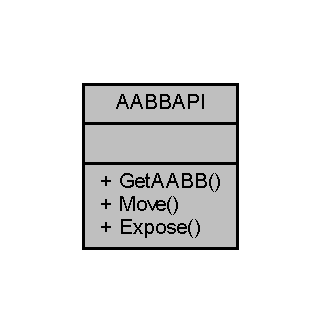
\includegraphics[width=154pt]{class_a_a_b_b_a_p_i__coll__graph}
\end{center}
\end{figure}
\subsection*{Static Public Member Functions}
\begin{DoxyCompactItemize}
\item 
static \hyperlink{_lua_context_8h_a2220f03700ba40e366f0ee2d684d5c91}{Lua\+Ref} \hyperlink{class_a_a_b_b_a_p_i_ad3b7d97acd59d1a83b1cc1ecc1d6f3a3}{Get\+A\+A\+BB} (int handle, \hyperlink{_lua_context_8h_a2ffcc2d3ed21165072a1d7b61259bf14}{Lua\+Context\+Handle} c\+Handle)
\begin{DoxyCompactList}\small\item\em Gets the aabb from an object instance handle. \end{DoxyCompactList}\item 
static \hyperlink{_lua_context_8h_a2220f03700ba40e366f0ee2d684d5c91}{Lua\+Ref} \hyperlink{class_a_a_b_b_a_p_i_aa832a0bc68a14f90c48ac4cd85663371}{Move} (\hyperlink{_lua_context_8h_a2220f03700ba40e366f0ee2d684d5c91}{Lua\+Ref} bbox, \hyperlink{_lua_context_8h_a2220f03700ba40e366f0ee2d684d5c91}{Lua\+Ref} old\+Pos, \hyperlink{_lua_context_8h_a2220f03700ba40e366f0ee2d684d5c91}{Lua\+Ref} new\+Pos, \hyperlink{_lua_context_8h_a2ffcc2d3ed21165072a1d7b61259bf14}{Lua\+Context\+Handle} c\+Handle)
\begin{DoxyCompactList}\small\item\em Moves the specified bbox. \end{DoxyCompactList}\item 
static void \hyperlink{class_a_a_b_b_a_p_i_a42a1a851b7ade27307e59ae2717bee02}{Expose} (\hyperlink{_lua_context_8h_a2ffcc2d3ed21165072a1d7b61259bf14}{Lua\+Context\+Handle} context\+Handle, \hyperlink{_types_8h_ad453f9f71ce1f9153fb748d6bb25e454}{string} lua\+A\+P\+I\+Name)
\begin{DoxyCompactList}\small\item\em Exposes the specified context handle. \end{DoxyCompactList}\end{DoxyCompactItemize}


\subsection{Detailed Description}


Definition at line 19 of file A\+A\+B\+B\+A\+P\+I.\+h.



\subsection{Member Function Documentation}
\index{A\+A\+B\+B\+A\+PI@{A\+A\+B\+B\+A\+PI}!Expose@{Expose}}
\index{Expose@{Expose}!A\+A\+B\+B\+A\+PI@{A\+A\+B\+B\+A\+PI}}
\subsubsection[{\texorpdfstring{Expose(\+Lua\+Context\+Handle context\+Handle, string lua\+A\+P\+I\+Name)}{Expose(LuaContextHandle contextHandle, string luaAPIName)}}]{\setlength{\rightskip}{0pt plus 5cm}void A\+A\+B\+B\+A\+P\+I\+::\+Expose (
\begin{DoxyParamCaption}
\item[{{\bf Lua\+Context\+Handle}}]{context\+Handle, }
\item[{{\bf string}}]{lua\+A\+P\+I\+Name}
\end{DoxyParamCaption}
)\hspace{0.3cm}{\ttfamily [static]}}\hypertarget{class_a_a_b_b_a_p_i_a42a1a851b7ade27307e59ae2717bee02}{}\label{class_a_a_b_b_a_p_i_a42a1a851b7ade27307e59ae2717bee02}


Exposes the specified context handle. 


\begin{DoxyParams}{Parameters}
{\em context\+Handle} & The context handle.\\
\hline
{\em lua\+A\+P\+I\+Name} & Name of the lua A\+PI.\\
\hline
\end{DoxyParams}


Definition at line 37 of file A\+A\+B\+B\+A\+P\+I.\+cpp.


\begin{DoxyCode}
38 \{
39 
40         \hyperlink{class_lua_context}{LuaContext}* pContext = \hyperlink{class_singleton_a74f32751d99bf3cc95fe17aba11f4b07}{LuaManager::GetInstance}().
      \hyperlink{class_lua_manager_a68592b46a59219d130cf4f637c977378}{GetContext}(contextHandle);
41         pContext->\hyperlink{class_lua_context_a2229908b6b329ed67105f1be7409cb3f}{ExposeFunction}(luaAPIName, \textcolor{stringliteral}{"getAABB"}, \hyperlink{class_a_a_b_b_a_p_i_ad3b7d97acd59d1a83b1cc1ecc1d6f3a3}{GetAABB});
42         pContext->\hyperlink{class_lua_context_a2229908b6b329ed67105f1be7409cb3f}{ExposeFunction}(luaAPIName, \textcolor{stringliteral}{"move"}, \hyperlink{class_a_a_b_b_a_p_i_aa832a0bc68a14f90c48ac4cd85663371}{Move});
43 
44 \}\end{DoxyCode}
\index{A\+A\+B\+B\+A\+PI@{A\+A\+B\+B\+A\+PI}!Get\+A\+A\+BB@{Get\+A\+A\+BB}}
\index{Get\+A\+A\+BB@{Get\+A\+A\+BB}!A\+A\+B\+B\+A\+PI@{A\+A\+B\+B\+A\+PI}}
\subsubsection[{\texorpdfstring{Get\+A\+A\+B\+B(int handle, Lua\+Context\+Handle c\+Handle)}{GetAABB(int handle, LuaContextHandle cHandle)}}]{\setlength{\rightskip}{0pt plus 5cm}{\bf Lua\+Ref} A\+A\+B\+B\+A\+P\+I\+::\+Get\+A\+A\+BB (
\begin{DoxyParamCaption}
\item[{int}]{handle, }
\item[{{\bf Lua\+Context\+Handle}}]{c\+Handle}
\end{DoxyParamCaption}
)\hspace{0.3cm}{\ttfamily [static]}}\hypertarget{class_a_a_b_b_a_p_i_ad3b7d97acd59d1a83b1cc1ecc1d6f3a3}{}\label{class_a_a_b_b_a_p_i_ad3b7d97acd59d1a83b1cc1ecc1d6f3a3}


Gets the aabb from an object instance handle. 


\begin{DoxyParams}{Parameters}
{\em handle} & The object instance handle.\\
\hline
{\em c\+Handle} & The context handle.\\
\hline
\end{DoxyParams}
\begin{DoxyReturn}{Returns}

\end{DoxyReturn}


Definition at line 5 of file A\+A\+B\+B\+A\+P\+I.\+cpp.


\begin{DoxyCode}
6 \{
7     \hyperlink{_lua_context_8h_a2220f03700ba40e366f0ee2d684d5c91}{LuaRef} AABBtable = luabridge::newTable(\hyperlink{class_singleton_a74f32751d99bf3cc95fe17aba11f4b07}{LuaManager::GetInstance}().
      GetContext(cHandle)->GetLuaState());
8     std::vector<vec3> bbox = \hyperlink{class_singleton_a74f32751d99bf3cc95fe17aba11f4b07}{LuaObjectInstanceManager::GetInstance}(
      cHandle)->GetRenderableObject()->GetAABB();
9 
10     AABBtable[\textcolor{stringliteral}{"min"}] = \hyperlink{_math_a_p_i_8h_a6d4bdd6987400be64a6a029dbf3e5fb2}{ToLuaTable}(bbox[0],cHandle);
11     AABBtable[\textcolor{stringliteral}{"max"}] = \hyperlink{_math_a_p_i_8h_a6d4bdd6987400be64a6a029dbf3e5fb2}{ToLuaTable}(bbox[1],cHandle);
12 
13     \textcolor{keywordflow}{return} AABBtable;
14 \}
\end{DoxyCode}
\index{A\+A\+B\+B\+A\+PI@{A\+A\+B\+B\+A\+PI}!Move@{Move}}
\index{Move@{Move}!A\+A\+B\+B\+A\+PI@{A\+A\+B\+B\+A\+PI}}
\subsubsection[{\texorpdfstring{Move(\+Lua\+Ref bbox, Lua\+Ref old\+Pos, Lua\+Ref new\+Pos, Lua\+Context\+Handle c\+Handle)}{Move(LuaRef bbox, LuaRef oldPos, LuaRef newPos, LuaContextHandle cHandle)}}]{\setlength{\rightskip}{0pt plus 5cm}{\bf Lua\+Ref} A\+A\+B\+B\+A\+P\+I\+::\+Move (
\begin{DoxyParamCaption}
\item[{{\bf Lua\+Ref}}]{bbox, }
\item[{{\bf Lua\+Ref}}]{old\+Pos, }
\item[{{\bf Lua\+Ref}}]{new\+Pos, }
\item[{{\bf Lua\+Context\+Handle}}]{c\+Handle}
\end{DoxyParamCaption}
)\hspace{0.3cm}{\ttfamily [static]}}\hypertarget{class_a_a_b_b_a_p_i_aa832a0bc68a14f90c48ac4cd85663371}{}\label{class_a_a_b_b_a_p_i_aa832a0bc68a14f90c48ac4cd85663371}


Moves the specified bbox. 


\begin{DoxyParams}{Parameters}
{\em bbox} & The bbox.\\
\hline
{\em old\+Pos} & The old position.\\
\hline
{\em new\+Pos} & The new position.\\
\hline
{\em c\+Handle} & The context handle.\\
\hline
\end{DoxyParams}
\begin{DoxyReturn}{Returns}

\end{DoxyReturn}


Definition at line 16 of file A\+A\+B\+B\+A\+P\+I.\+cpp.


\begin{DoxyCode}
17 \{
18     \hyperlink{_types_8h_a3d0ce73e3199de81565fb01632415288}{vec3} bboxmin = \hyperlink{_math_a_p_i_8h_a57e551c31a30e104a0c0ca525557f265}{FromLuaTable<vec3>} (bbox[\textcolor{stringliteral}{"min"}]);
19     \hyperlink{_types_8h_a3d0ce73e3199de81565fb01632415288}{vec3} bboxmax = \hyperlink{_math_a_p_i_8h_a57e551c31a30e104a0c0ca525557f265}{FromLuaTable<vec3>}(bbox[\textcolor{stringliteral}{"max"}]);
20     \hyperlink{_types_8h_a3d0ce73e3199de81565fb01632415288}{vec3} oldposvec = \hyperlink{_math_a_p_i_8h_a57e551c31a30e104a0c0ca525557f265}{FromLuaTable<vec3>}(oldPos);
21     \hyperlink{_types_8h_a3d0ce73e3199de81565fb01632415288}{vec3} newposvec = \hyperlink{_math_a_p_i_8h_a57e551c31a30e104a0c0ca525557f265}{FromLuaTable<vec3>}(newPos);
22 
23     \hyperlink{_types_8h_a3d0ce73e3199de81565fb01632415288}{vec3} diff = (newposvec - oldposvec);
24     \hyperlink{_types_8h_a3d0ce73e3199de81565fb01632415288}{vec3} newMin = bboxmin + diff;
25     \hyperlink{_types_8h_a3d0ce73e3199de81565fb01632415288}{vec3} newMax = bboxmax + diff;
26 
27 
28     \hyperlink{_lua_context_8h_a2220f03700ba40e366f0ee2d684d5c91}{LuaRef} newAABB = luabridge::newTable(\hyperlink{class_singleton_a74f32751d99bf3cc95fe17aba11f4b07}{LuaManager::GetInstance}().GetContext(
      cHandle)->GetLuaState());
29 
30     newAABB[\textcolor{stringliteral}{"min"}] = \hyperlink{_math_a_p_i_8h_a6d4bdd6987400be64a6a029dbf3e5fb2}{ToLuaTable}(newMin,cHandle);
31     newAABB[\textcolor{stringliteral}{"max"}] = \hyperlink{_math_a_p_i_8h_a6d4bdd6987400be64a6a029dbf3e5fb2}{ToLuaTable}(newMax,cHandle);
32 
33     \textcolor{keywordflow}{return} newAABB;
34 \}
\end{DoxyCode}


The documentation for this class was generated from the following files\+:\begin{DoxyCompactItemize}
\item 
C\+:/\+Users/elizabeth/\+Documents/\+Git\+Hub/\+Engine/\+Open\+G\+L\+Engine/\+Open\+G\+L\+Engine/\hyperlink{_a_a_b_b_a_p_i_8h}{A\+A\+B\+B\+A\+P\+I.\+h}\item 
C\+:/\+Users/elizabeth/\+Documents/\+Git\+Hub/\+Engine/\+Open\+G\+L\+Engine/\+Open\+G\+L\+Engine/\hyperlink{_a_a_b_b_a_p_i_8cpp}{A\+A\+B\+B\+A\+P\+I.\+cpp}\end{DoxyCompactItemize}

\hypertarget{class_additive_blend_effect}{}\section{Additive\+Blend\+Effect Class Reference}
\label{class_additive_blend_effect}\index{Additive\+Blend\+Effect@{Additive\+Blend\+Effect}}


{\ttfamily \#include $<$Additive\+Blend\+Effect.\+h$>$}



Collaboration diagram for Additive\+Blend\+Effect\+:\nopagebreak
\begin{figure}[H]
\begin{center}
\leavevmode
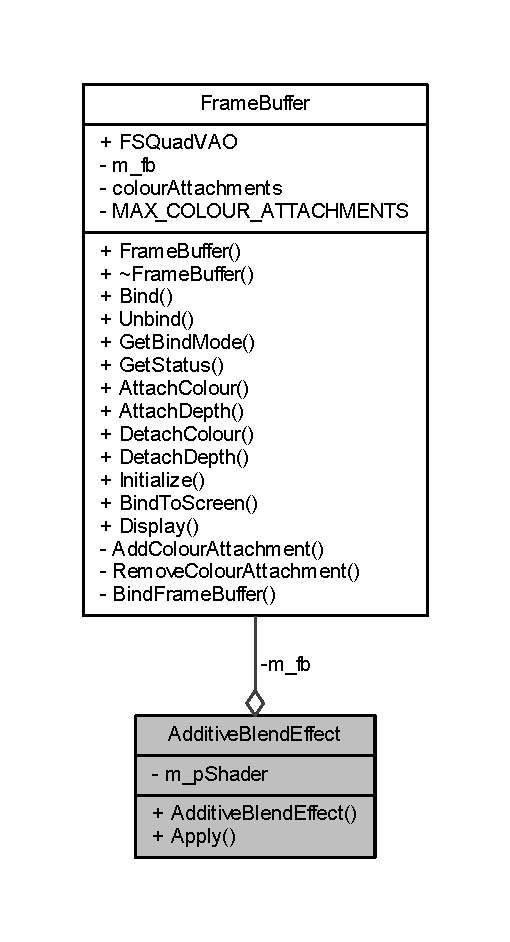
\includegraphics[width=245pt]{class_additive_blend_effect__coll__graph}
\end{center}
\end{figure}
\subsection*{Public Member Functions}
\begin{DoxyCompactItemize}
\item 
\hyperlink{class_additive_blend_effect_ac66ffc77617ad66c5bc5cf9811906c66}{Additive\+Blend\+Effect} ()
\begin{DoxyCompactList}\small\item\em Initializes a new instance of the \hyperlink{class_additive_blend_effect}{Additive\+Blend\+Effect} class. \end{DoxyCompactList}\item 
void \hyperlink{class_additive_blend_effect_a9e75b87d6e8bf28acc4f5d31c3049453}{Apply} (G\+Luint input\+Tex0, G\+Luint input\+Tex1, G\+Luint output\+Tex)
\begin{DoxyCompactList}\small\item\em Applies the additive blend effect. \end{DoxyCompactList}\end{DoxyCompactItemize}
\subsection*{Private Attributes}
\begin{DoxyCompactItemize}
\item 
\hyperlink{class_frame_buffer}{Frame\+Buffer} \hyperlink{class_additive_blend_effect_aa047c3ebbd318f3faee9dc17b63680e7}{m\+\_\+fb}
\begin{DoxyCompactList}\small\item\em The frame buffer \end{DoxyCompactList}\item 
std\+::unique\+\_\+ptr$<$ \hyperlink{class_i_shader}{I\+Shader} $>$ const \& \hyperlink{class_additive_blend_effect_a5f25db987222e0f6cefb14116da373e9}{m\+\_\+p\+Shader}
\begin{DoxyCompactList}\small\item\em The shader \end{DoxyCompactList}\end{DoxyCompactItemize}


\subsection{Detailed Description}


Definition at line 17 of file Additive\+Blend\+Effect.\+h.



\subsection{Constructor \& Destructor Documentation}
\index{Additive\+Blend\+Effect@{Additive\+Blend\+Effect}!Additive\+Blend\+Effect@{Additive\+Blend\+Effect}}
\index{Additive\+Blend\+Effect@{Additive\+Blend\+Effect}!Additive\+Blend\+Effect@{Additive\+Blend\+Effect}}
\subsubsection[{\texorpdfstring{Additive\+Blend\+Effect()}{AdditiveBlendEffect()}}]{\setlength{\rightskip}{0pt plus 5cm}Additive\+Blend\+Effect\+::\+Additive\+Blend\+Effect (
\begin{DoxyParamCaption}
{}
\end{DoxyParamCaption}
)}\hypertarget{class_additive_blend_effect_ac66ffc77617ad66c5bc5cf9811906c66}{}\label{class_additive_blend_effect_ac66ffc77617ad66c5bc5cf9811906c66}


Initializes a new instance of the \hyperlink{class_additive_blend_effect}{Additive\+Blend\+Effect} class. 



Definition at line 5 of file Additive\+Blend\+Effect.\+cpp.



References Additive\+Blend\+Effect().



Referenced by Additive\+Blend\+Effect().


\begin{DoxyCode}
6   : \hyperlink{class_additive_blend_effect_a5f25db987222e0f6cefb14116da373e9}{m\_pShader}(\hyperlink{class_singleton_a74f32751d99bf3cc95fe17aba11f4b07}{ShaderLibrary::GetInstance}().GetShader(\textcolor{stringliteral}{"
      AdditiveBlendEffect"}))
7 \{
8 
9 \}
\end{DoxyCode}


Here is the call graph for this function\+:\nopagebreak
\begin{figure}[H]
\begin{center}
\leavevmode
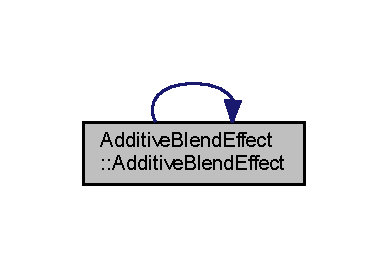
\includegraphics[width=186pt]{class_additive_blend_effect_ac66ffc77617ad66c5bc5cf9811906c66_cgraph}
\end{center}
\end{figure}




Here is the caller graph for this function\+:\nopagebreak
\begin{figure}[H]
\begin{center}
\leavevmode
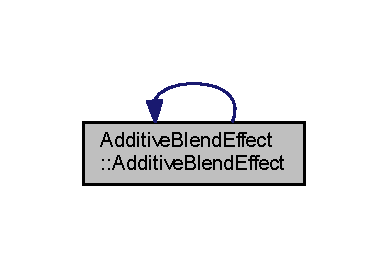
\includegraphics[width=186pt]{class_additive_blend_effect_ac66ffc77617ad66c5bc5cf9811906c66_icgraph}
\end{center}
\end{figure}




\subsection{Member Function Documentation}
\index{Additive\+Blend\+Effect@{Additive\+Blend\+Effect}!Apply@{Apply}}
\index{Apply@{Apply}!Additive\+Blend\+Effect@{Additive\+Blend\+Effect}}
\subsubsection[{\texorpdfstring{Apply(\+G\+Luint input\+Tex0, G\+Luint input\+Tex1, G\+Luint output\+Tex)}{Apply(GLuint inputTex0, GLuint inputTex1, GLuint outputTex)}}]{\setlength{\rightskip}{0pt plus 5cm}void Additive\+Blend\+Effect\+::\+Apply (
\begin{DoxyParamCaption}
\item[{G\+Luint}]{input\+Tex0, }
\item[{G\+Luint}]{input\+Tex1, }
\item[{G\+Luint}]{output\+Tex}
\end{DoxyParamCaption}
)}\hypertarget{class_additive_blend_effect_a9e75b87d6e8bf28acc4f5d31c3049453}{}\label{class_additive_blend_effect_a9e75b87d6e8bf28acc4f5d31c3049453}


Applies the additive blend effect. 


\begin{DoxyParams}{Parameters}
{\em input\+Tex0} & The input tex0.\\
\hline
{\em input\+Tex1} & The input tex1.\\
\hline
{\em output\+Tex} & The output tex.\\
\hline
\end{DoxyParams}


Definition at line 11 of file Additive\+Blend\+Effect.\+cpp.


\begin{DoxyCode}
12 \{
13   \hyperlink{class_additive_blend_effect_aa047c3ebbd318f3faee9dc17b63680e7}{m\_fb}.\hyperlink{class_frame_buffer_ae7e61568475fba3b15e446c9061833ea}{Bind}();
14 
15   \hyperlink{class_additive_blend_effect_aa047c3ebbd318f3faee9dc17b63680e7}{m\_fb}.\hyperlink{class_frame_buffer_a1556417c0dec00d1d24bdf0e84bc4c4d}{AttachColour}(0, outputTex);
16   glClear(GL\_COLOR\_BUFFER\_BIT | GL\_DEPTH\_BUFFER\_BIT);
17   \hyperlink{class_additive_blend_effect_a5f25db987222e0f6cefb14116da373e9}{m\_pShader}->Bind();
18   glBindVertexArray(\hyperlink{class_frame_buffer_a22b0c9de2bef06e0de865684556a6677}{FrameBuffer::FSQuadVAO});
19 
20   glActiveTexture(GL\_TEXTURE0 + 0);
21   glBindTexture(GL\_TEXTURE\_2D, inputTex0);
22   \hyperlink{class_additive_blend_effect_a5f25db987222e0f6cefb14116da373e9}{m\_pShader}->TransmitUniform(\textcolor{stringliteral}{"inputTex0"}, 0);
23 
24   glActiveTexture(GL\_TEXTURE0 + 1);
25   glBindTexture(GL\_TEXTURE\_2D, inputTex1);
26   \hyperlink{class_additive_blend_effect_a5f25db987222e0f6cefb14116da373e9}{m\_pShader}->TransmitUniform(\textcolor{stringliteral}{"inputTex1"}, 1);
27 
28   glDrawArrays(GL\_QUADS, 0, 4);
29   glBindVertexArray(NULL);
30 
31   \hyperlink{class_additive_blend_effect_aa047c3ebbd318f3faee9dc17b63680e7}{m\_fb}.\hyperlink{class_frame_buffer_a1e114b325998ec4e4b9a9ea090d64ae8}{Unbind}();
32 \}
\end{DoxyCode}


\subsection{Member Data Documentation}
\index{Additive\+Blend\+Effect@{Additive\+Blend\+Effect}!m\+\_\+fb@{m\+\_\+fb}}
\index{m\+\_\+fb@{m\+\_\+fb}!Additive\+Blend\+Effect@{Additive\+Blend\+Effect}}
\subsubsection[{\texorpdfstring{m\+\_\+fb}{m_fb}}]{\setlength{\rightskip}{0pt plus 5cm}{\bf Frame\+Buffer} Additive\+Blend\+Effect\+::m\+\_\+fb\hspace{0.3cm}{\ttfamily [private]}}\hypertarget{class_additive_blend_effect_aa047c3ebbd318f3faee9dc17b63680e7}{}\label{class_additive_blend_effect_aa047c3ebbd318f3faee9dc17b63680e7}


The frame buffer 



Definition at line 39 of file Additive\+Blend\+Effect.\+h.

\index{Additive\+Blend\+Effect@{Additive\+Blend\+Effect}!m\+\_\+p\+Shader@{m\+\_\+p\+Shader}}
\index{m\+\_\+p\+Shader@{m\+\_\+p\+Shader}!Additive\+Blend\+Effect@{Additive\+Blend\+Effect}}
\subsubsection[{\texorpdfstring{m\+\_\+p\+Shader}{m_pShader}}]{\setlength{\rightskip}{0pt plus 5cm}std\+::unique\+\_\+ptr$<${\bf I\+Shader}$>$ const\& Additive\+Blend\+Effect\+::m\+\_\+p\+Shader\hspace{0.3cm}{\ttfamily [private]}}\hypertarget{class_additive_blend_effect_a5f25db987222e0f6cefb14116da373e9}{}\label{class_additive_blend_effect_a5f25db987222e0f6cefb14116da373e9}


The shader 



Definition at line 44 of file Additive\+Blend\+Effect.\+h.



The documentation for this class was generated from the following files\+:\begin{DoxyCompactItemize}
\item 
C\+:/\+Users/elizabeth/\+Documents/\+Git\+Hub/\+Engine/\+Open\+G\+L\+Engine/\+Open\+G\+L\+Engine/\hyperlink{_additive_blend_effect_8h}{Additive\+Blend\+Effect.\+h}\item 
C\+:/\+Users/elizabeth/\+Documents/\+Git\+Hub/\+Engine/\+Open\+G\+L\+Engine/\+Open\+G\+L\+Engine/\hyperlink{_additive_blend_effect_8cpp}{Additive\+Blend\+Effect.\+cpp}\end{DoxyCompactItemize}

\hypertarget{class_affine_transformable}{}\section{Affine\+Transformable Class Reference}
\label{class_affine_transformable}\index{Affine\+Transformable@{Affine\+Transformable}}


{\ttfamily \#include $<$Affine\+Transformable.\+h$>$}



Inheritance diagram for Affine\+Transformable\+:\nopagebreak
\begin{figure}[H]
\begin{center}
\leavevmode
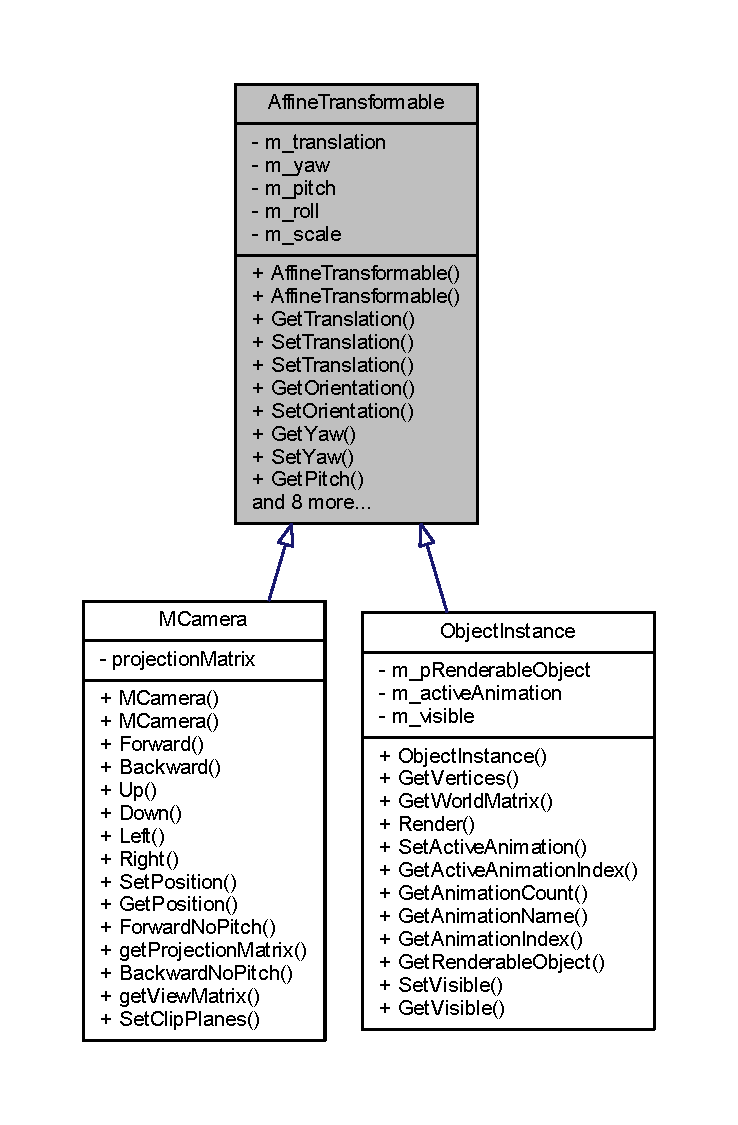
\includegraphics[width=350pt]{class_affine_transformable__inherit__graph}
\end{center}
\end{figure}


Collaboration diagram for Affine\+Transformable\+:\nopagebreak
\begin{figure}[H]
\begin{center}
\leavevmode
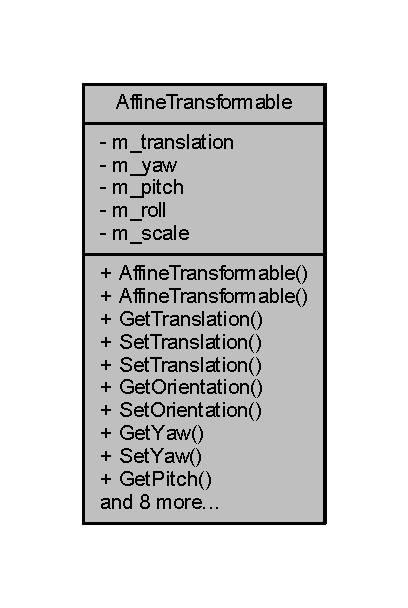
\includegraphics[width=196pt]{class_affine_transformable__coll__graph}
\end{center}
\end{figure}
\subsection*{Public Member Functions}
\begin{DoxyCompactItemize}
\item 
\hyperlink{class_affine_transformable_a54fbbe0cdde13ea581dce04ec0de8545}{Affine\+Transformable} ()
\begin{DoxyCompactList}\small\item\em Initializes a new instance of the \hyperlink{class_affine_transformable}{Affine\+Transformable} class. \end{DoxyCompactList}\item 
\hyperlink{class_affine_transformable_ab70fc4cbb5d5d3436d4e6fc50ccb1cc7}{Affine\+Transformable} (\hyperlink{_types_8h_a3d0ce73e3199de81565fb01632415288}{vec3} const \&translation, float yaw, float pitch, float roll, \hyperlink{_types_8h_a3d0ce73e3199de81565fb01632415288}{vec3} const \&scale)
\begin{DoxyCompactList}\small\item\em Initializes a new instance of the \hyperlink{class_affine_transformable}{Affine\+Transformable} class. \end{DoxyCompactList}\item 
\hyperlink{_types_8h_a3d0ce73e3199de81565fb01632415288}{vec3} const \& \hyperlink{class_affine_transformable_a6c6a849bb0dc120cdb96494aa40c6898}{Get\+Translation} () const 
\begin{DoxyCompactList}\small\item\em Gets the translation. \end{DoxyCompactList}\item 
void \hyperlink{class_affine_transformable_abd554f0c81205675ed2a6520e09e5b98}{Set\+Translation} (\hyperlink{_types_8h_a3d0ce73e3199de81565fb01632415288}{vec3} const \&translation)
\begin{DoxyCompactList}\small\item\em Sets the translation. \end{DoxyCompactList}\item 
void \hyperlink{class_affine_transformable_a47eccc886862946587d6e9de46f55dff}{Set\+Translation} (float x, float y, float z)
\begin{DoxyCompactList}\small\item\em Sets the translation. \end{DoxyCompactList}\item 
\hyperlink{_types_8h_a2db59f395fe82a7394c6324956c265d8}{mat4} const \& \hyperlink{class_affine_transformable_a891419484ac01da747f832e5a84e8e37}{Get\+Orientation} () const 
\begin{DoxyCompactList}\small\item\em Gets the orientation. \end{DoxyCompactList}\item 
void \hyperlink{class_affine_transformable_a9565967f58321117e198b6925c4200d6}{Set\+Orientation} (float deg\+Yaw, float deg\+Pitch, float deg\+Roll)
\begin{DoxyCompactList}\small\item\em Sets the orientation. \end{DoxyCompactList}\item 
float \hyperlink{class_affine_transformable_afcc35bdd6301a92f87d339f386743d93}{Get\+Yaw} () const 
\begin{DoxyCompactList}\small\item\em Gets the yaw. \end{DoxyCompactList}\item 
void \hyperlink{class_affine_transformable_a47ab5b07df1ee77ae2e63dc0804c5caa}{Set\+Yaw} (float deg\+Yaw)
\begin{DoxyCompactList}\small\item\em Sets the yaw. \end{DoxyCompactList}\item 
float \hyperlink{class_affine_transformable_ae2905ed9fc069a5b237a7103538723d3}{Get\+Pitch} () const 
\begin{DoxyCompactList}\small\item\em Gets the pitch. \end{DoxyCompactList}\item 
void \hyperlink{class_affine_transformable_a8413b02e25aec2a759d5fd269d13fc02}{Set\+Pitch} (float deg\+Pitch)
\begin{DoxyCompactList}\small\item\em Sets the pitch. \end{DoxyCompactList}\item 
float \hyperlink{class_affine_transformable_a36e3c2f2b62a4a66ab960118440d186c}{Get\+Roll} () const 
\begin{DoxyCompactList}\small\item\em Gets the roll. \end{DoxyCompactList}\item 
void \hyperlink{class_affine_transformable_a9db54f563d9db087b43b64a371200264}{Set\+Roll} (float deg\+Roll)
\begin{DoxyCompactList}\small\item\em Sets the roll. \end{DoxyCompactList}\item 
\hyperlink{_types_8h_a3d0ce73e3199de81565fb01632415288}{vec3} const \& \hyperlink{class_affine_transformable_a8a9e32647f5e4bfb893d63ff8fb9b9f8}{Get\+Scale} () const 
\begin{DoxyCompactList}\small\item\em Gets the scale. \end{DoxyCompactList}\item 
void \hyperlink{class_affine_transformable_a215383be79781d61103dfdf8c201be22}{Set\+Scale} (\hyperlink{_types_8h_a3d0ce73e3199de81565fb01632415288}{vec3} const \&scale)
\begin{DoxyCompactList}\small\item\em Sets the scale. \end{DoxyCompactList}\item 
\hyperlink{_types_8h_a2db59f395fe82a7394c6324956c265d8}{mat4} \hyperlink{class_affine_transformable_a3eb990ab0b75ad30d3bb667e437d8606}{Get\+Transform} () const 
\begin{DoxyCompactList}\small\item\em Gets the transform. \end{DoxyCompactList}\item 
void \hyperlink{class_affine_transformable_aacc67804c045aa75da888ca3ea409939}{Set\+Transform} (\hyperlink{_types_8h_a2db59f395fe82a7394c6324956c265d8}{mat4} const \&transform)
\begin{DoxyCompactList}\small\item\em Sets the transform. \end{DoxyCompactList}\item 
void \hyperlink{class_affine_transformable_ac4faa6d4c8127e61622ae265ba708276}{Set\+Transform} (\hyperlink{_types_8h_a3d0ce73e3199de81565fb01632415288}{vec3} const \&translation, float yaw, float pitch, float roll, \hyperlink{_types_8h_a3d0ce73e3199de81565fb01632415288}{vec3} const \&scale)
\begin{DoxyCompactList}\small\item\em Sets the transform. \end{DoxyCompactList}\end{DoxyCompactItemize}
\subsection*{Private Attributes}
\begin{DoxyCompactItemize}
\item 
\hyperlink{_types_8h_a3d0ce73e3199de81565fb01632415288}{vec3} \hyperlink{class_affine_transformable_a3573983127e380c3d9151c32b43d199d}{m\+\_\+translation}
\begin{DoxyCompactList}\small\item\em The translation \end{DoxyCompactList}\item 
float \hyperlink{class_affine_transformable_abf9b231dc1bd3e61bbbed8714f127f93}{m\+\_\+yaw}
\begin{DoxyCompactList}\small\item\em The yaw \end{DoxyCompactList}\item 
float \hyperlink{class_affine_transformable_ade24cef424ce102502357cde8214d54b}{m\+\_\+pitch}
\begin{DoxyCompactList}\small\item\em The pitch \end{DoxyCompactList}\item 
float \hyperlink{class_affine_transformable_a33e3fc9a32cafaa0a04c6058f283d437}{m\+\_\+roll}
\begin{DoxyCompactList}\small\item\em The roll \end{DoxyCompactList}\item 
\hyperlink{_types_8h_a3d0ce73e3199de81565fb01632415288}{vec3} \hyperlink{class_affine_transformable_ac332af15336f089337fd31d7b3996bad}{m\+\_\+scale}
\begin{DoxyCompactList}\small\item\em The scale \end{DoxyCompactList}\end{DoxyCompactItemize}


\subsection{Detailed Description}


Definition at line 16 of file Affine\+Transformable.\+h.



\subsection{Constructor \& Destructor Documentation}
\index{Affine\+Transformable@{Affine\+Transformable}!Affine\+Transformable@{Affine\+Transformable}}
\index{Affine\+Transformable@{Affine\+Transformable}!Affine\+Transformable@{Affine\+Transformable}}
\subsubsection[{\texorpdfstring{Affine\+Transformable()}{AffineTransformable()}}]{\setlength{\rightskip}{0pt plus 5cm}Affine\+Transformable\+::\+Affine\+Transformable (
\begin{DoxyParamCaption}
{}
\end{DoxyParamCaption}
)}\hypertarget{class_affine_transformable_a54fbbe0cdde13ea581dce04ec0de8545}{}\label{class_affine_transformable_a54fbbe0cdde13ea581dce04ec0de8545}


Initializes a new instance of the \hyperlink{class_affine_transformable}{Affine\+Transformable} class. 



Definition at line 12 of file Affine\+Transformable.\+cpp.



References Affine\+Transformable(), m\+\_\+translation, and Set\+Orientation().



Referenced by Affine\+Transformable(), and M\+Camera\+::\+M\+Camera().


\begin{DoxyCode}
13   : \hyperlink{class_affine_transformable_a3573983127e380c3d9151c32b43d199d}{m\_translation}(0)
14   , \hyperlink{class_affine_transformable_ac332af15336f089337fd31d7b3996bad}{m\_scale}(1, 1, 1)
15 \{
16   \hyperlink{class_affine_transformable_a9565967f58321117e198b6925c4200d6}{SetOrientation}(0, 0, 0);
17 \}
\end{DoxyCode}


Here is the call graph for this function\+:\nopagebreak
\begin{figure}[H]
\begin{center}
\leavevmode
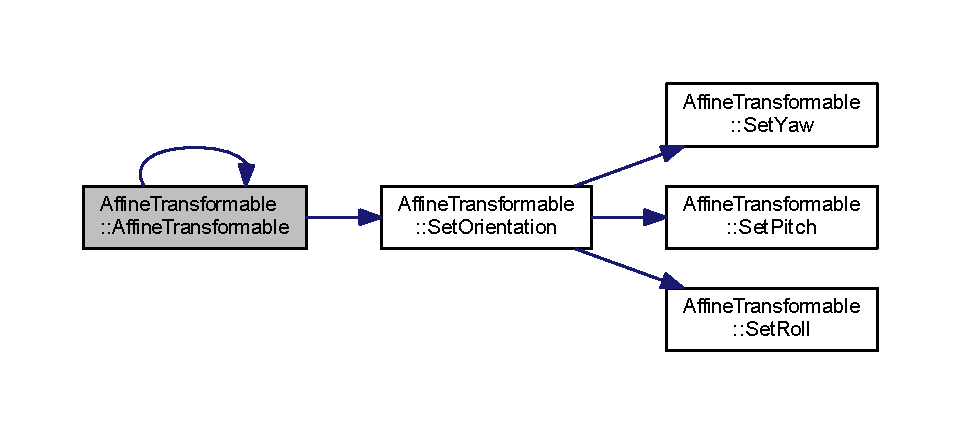
\includegraphics[width=350pt]{class_affine_transformable_a54fbbe0cdde13ea581dce04ec0de8545_cgraph}
\end{center}
\end{figure}




Here is the caller graph for this function\+:\nopagebreak
\begin{figure}[H]
\begin{center}
\leavevmode
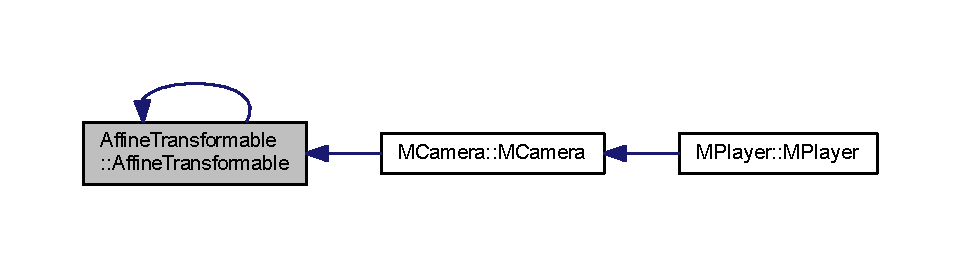
\includegraphics[width=350pt]{class_affine_transformable_a54fbbe0cdde13ea581dce04ec0de8545_icgraph}
\end{center}
\end{figure}


\index{Affine\+Transformable@{Affine\+Transformable}!Affine\+Transformable@{Affine\+Transformable}}
\index{Affine\+Transformable@{Affine\+Transformable}!Affine\+Transformable@{Affine\+Transformable}}
\subsubsection[{\texorpdfstring{Affine\+Transformable(vec3 const \&translation, float yaw, float pitch, float roll, vec3 const \&scale)}{AffineTransformable(vec3 const &translation, float yaw, float pitch, float roll, vec3 const &scale)}}]{\setlength{\rightskip}{0pt plus 5cm}Affine\+Transformable\+::\+Affine\+Transformable (
\begin{DoxyParamCaption}
\item[{{\bf vec3} const \&}]{translation, }
\item[{float}]{yaw, }
\item[{float}]{pitch, }
\item[{float}]{roll, }
\item[{{\bf vec3} const \&}]{scale}
\end{DoxyParamCaption}
)}\hypertarget{class_affine_transformable_ab70fc4cbb5d5d3436d4e6fc50ccb1cc7}{}\label{class_affine_transformable_ab70fc4cbb5d5d3436d4e6fc50ccb1cc7}


Initializes a new instance of the \hyperlink{class_affine_transformable}{Affine\+Transformable} class. 


\begin{DoxyParams}{Parameters}
{\em translation} & The translation.\\
\hline
{\em yaw} & The yaw.\\
\hline
{\em pitch} & The pitch.\\
\hline
{\em roll} & The roll.\\
\hline
{\em scale} & The scale.\\
\hline
\end{DoxyParams}


Definition at line 5 of file Affine\+Transformable.\+cpp.



References Set\+Orientation(), Set\+Scale(), and Set\+Translation().


\begin{DoxyCode}
6 \{
7   \hyperlink{class_affine_transformable_abd554f0c81205675ed2a6520e09e5b98}{SetTranslation}(translation);
8   \hyperlink{class_affine_transformable_a9565967f58321117e198b6925c4200d6}{SetOrientation}(yaw, pitch, roll);
9   \hyperlink{class_affine_transformable_a215383be79781d61103dfdf8c201be22}{SetScale}(scale);
10 \}
\end{DoxyCode}


Here is the call graph for this function\+:\nopagebreak
\begin{figure}[H]
\begin{center}
\leavevmode
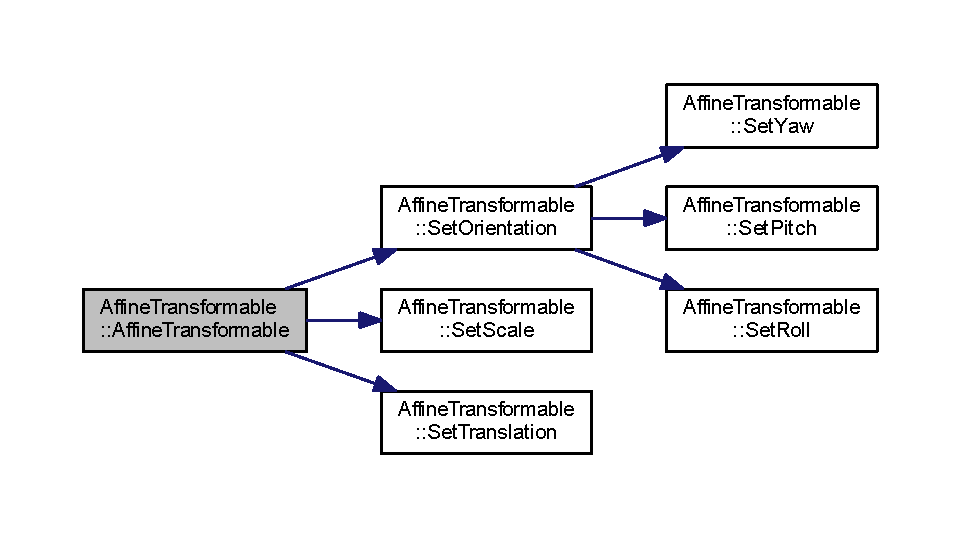
\includegraphics[width=350pt]{class_affine_transformable_ab70fc4cbb5d5d3436d4e6fc50ccb1cc7_cgraph}
\end{center}
\end{figure}




\subsection{Member Function Documentation}
\index{Affine\+Transformable@{Affine\+Transformable}!Get\+Orientation@{Get\+Orientation}}
\index{Get\+Orientation@{Get\+Orientation}!Affine\+Transformable@{Affine\+Transformable}}
\subsubsection[{\texorpdfstring{Get\+Orientation() const }{GetOrientation() const }}]{\setlength{\rightskip}{0pt plus 5cm}{\bf mat4} const \& Affine\+Transformable\+::\+Get\+Orientation (
\begin{DoxyParamCaption}
{}
\end{DoxyParamCaption}
) const}\hypertarget{class_affine_transformable_a891419484ac01da747f832e5a84e8e37}{}\label{class_affine_transformable_a891419484ac01da747f832e5a84e8e37}


Gets the orientation. 

\begin{DoxyReturn}{Returns}
mat4
\end{DoxyReturn}


Definition at line 34 of file Affine\+Transformable.\+cpp.



Referenced by Get\+Transform().


\begin{DoxyCode}
35 \{
36   \textcolor{keywordflow}{return} \hyperlink{_types_8h_a2db59f395fe82a7394c6324956c265d8}{mat4}(\hyperlink{_types_8h_a02abcac728eae225e929e9e0dc427f28}{quat}(\hyperlink{_types_8h_a3d0ce73e3199de81565fb01632415288}{vec3}(\hyperlink{class_affine_transformable_ade24cef424ce102502357cde8214d54b}{m\_pitch}, \hyperlink{class_affine_transformable_abf9b231dc1bd3e61bbbed8714f127f93}{m\_yaw}, \hyperlink{class_affine_transformable_a33e3fc9a32cafaa0a04c6058f283d437}{m\_roll})));
37 \}
\end{DoxyCode}


Here is the caller graph for this function\+:
\nopagebreak
\begin{figure}[H]
\begin{center}
\leavevmode
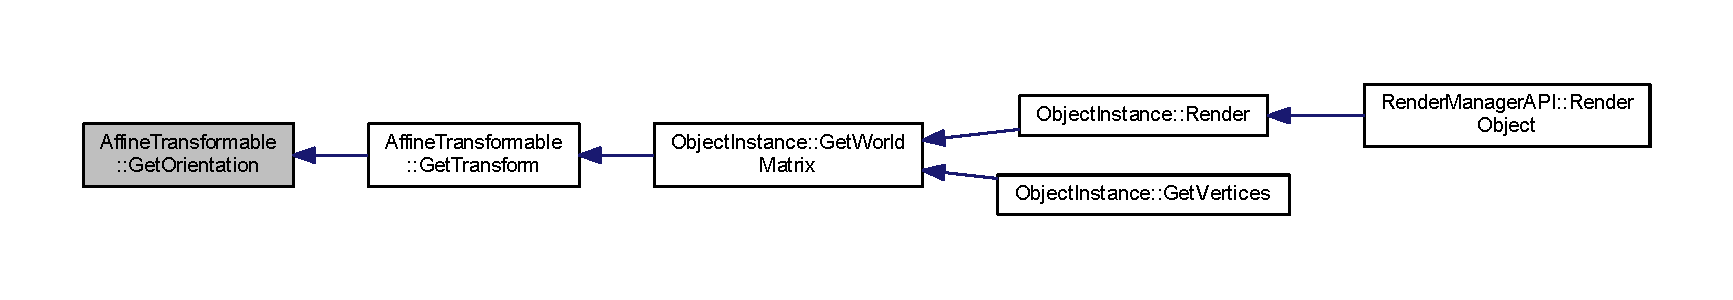
\includegraphics[width=350pt]{class_affine_transformable_a891419484ac01da747f832e5a84e8e37_icgraph}
\end{center}
\end{figure}


\index{Affine\+Transformable@{Affine\+Transformable}!Get\+Pitch@{Get\+Pitch}}
\index{Get\+Pitch@{Get\+Pitch}!Affine\+Transformable@{Affine\+Transformable}}
\subsubsection[{\texorpdfstring{Get\+Pitch() const }{GetPitch() const }}]{\setlength{\rightskip}{0pt plus 5cm}float Affine\+Transformable\+::\+Get\+Pitch (
\begin{DoxyParamCaption}
{}
\end{DoxyParamCaption}
) const}\hypertarget{class_affine_transformable_ae2905ed9fc069a5b237a7103538723d3}{}\label{class_affine_transformable_ae2905ed9fc069a5b237a7103538723d3}


Gets the pitch. 

\begin{DoxyReturn}{Returns}
float
\end{DoxyReturn}


Definition at line 56 of file Affine\+Transformable.\+cpp.



References m\+\_\+pitch.


\begin{DoxyCode}
57 \{
58   \textcolor{keywordflow}{return} \hyperlink{_m_math_8h_a8a41524e2041d1382fe880bedddd20a1}{RadToDeg}(\hyperlink{class_affine_transformable_ade24cef424ce102502357cde8214d54b}{m\_pitch});
59 \}
\end{DoxyCode}
\index{Affine\+Transformable@{Affine\+Transformable}!Get\+Roll@{Get\+Roll}}
\index{Get\+Roll@{Get\+Roll}!Affine\+Transformable@{Affine\+Transformable}}
\subsubsection[{\texorpdfstring{Get\+Roll() const }{GetRoll() const }}]{\setlength{\rightskip}{0pt plus 5cm}float Affine\+Transformable\+::\+Get\+Roll (
\begin{DoxyParamCaption}
{}
\end{DoxyParamCaption}
) const}\hypertarget{class_affine_transformable_a36e3c2f2b62a4a66ab960118440d186c}{}\label{class_affine_transformable_a36e3c2f2b62a4a66ab960118440d186c}


Gets the roll. 

\begin{DoxyReturn}{Returns}
float
\end{DoxyReturn}


Definition at line 66 of file Affine\+Transformable.\+cpp.



References m\+\_\+roll.


\begin{DoxyCode}
67 \{
68   \textcolor{keywordflow}{return} \hyperlink{_m_math_8h_a8a41524e2041d1382fe880bedddd20a1}{RadToDeg}(\hyperlink{class_affine_transformable_a33e3fc9a32cafaa0a04c6058f283d437}{m\_roll});
69 \}
\end{DoxyCode}
\index{Affine\+Transformable@{Affine\+Transformable}!Get\+Scale@{Get\+Scale}}
\index{Get\+Scale@{Get\+Scale}!Affine\+Transformable@{Affine\+Transformable}}
\subsubsection[{\texorpdfstring{Get\+Scale() const }{GetScale() const }}]{\setlength{\rightskip}{0pt plus 5cm}{\bf vec3} const \& Affine\+Transformable\+::\+Get\+Scale (
\begin{DoxyParamCaption}
{}
\end{DoxyParamCaption}
) const}\hypertarget{class_affine_transformable_a8a9e32647f5e4bfb893d63ff8fb9b9f8}{}\label{class_affine_transformable_a8a9e32647f5e4bfb893d63ff8fb9b9f8}


Gets the scale. 

\begin{DoxyReturn}{Returns}
vec3
\end{DoxyReturn}


Definition at line 76 of file Affine\+Transformable.\+cpp.



References m\+\_\+scale.



Referenced by Object\+Instance\+A\+P\+I\+::\+Get\+Scale().


\begin{DoxyCode}
77 \{
78   \textcolor{keywordflow}{return} \hyperlink{class_affine_transformable_ac332af15336f089337fd31d7b3996bad}{m\_scale};
79 \}
\end{DoxyCode}


Here is the caller graph for this function\+:\nopagebreak
\begin{figure}[H]
\begin{center}
\leavevmode
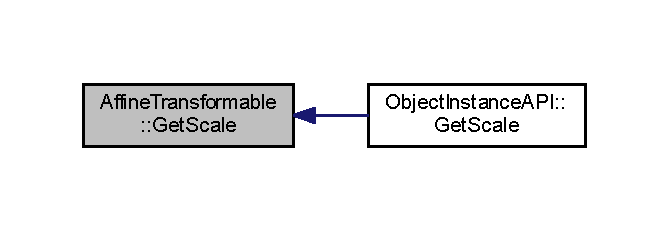
\includegraphics[width=321pt]{class_affine_transformable_a8a9e32647f5e4bfb893d63ff8fb9b9f8_icgraph}
\end{center}
\end{figure}


\index{Affine\+Transformable@{Affine\+Transformable}!Get\+Transform@{Get\+Transform}}
\index{Get\+Transform@{Get\+Transform}!Affine\+Transformable@{Affine\+Transformable}}
\subsubsection[{\texorpdfstring{Get\+Transform() const }{GetTransform() const }}]{\setlength{\rightskip}{0pt plus 5cm}{\bf mat4} Affine\+Transformable\+::\+Get\+Transform (
\begin{DoxyParamCaption}
{}
\end{DoxyParamCaption}
) const}\hypertarget{class_affine_transformable_a3eb990ab0b75ad30d3bb667e437d8606}{}\label{class_affine_transformable_a3eb990ab0b75ad30d3bb667e437d8606}


Gets the transform. 

\begin{DoxyReturn}{Returns}

\end{DoxyReturn}


Definition at line 86 of file Affine\+Transformable.\+cpp.



References Get\+Orientation().



Referenced by Object\+Instance\+::\+Get\+World\+Matrix().


\begin{DoxyCode}
87 \{
88   \hyperlink{_types_8h_a2db59f395fe82a7394c6324956c265d8}{mat4} translationMatrix = translate(\hyperlink{class_affine_transformable_a3573983127e380c3d9151c32b43d199d}{m\_translation});
89   \hyperlink{_types_8h_a2db59f395fe82a7394c6324956c265d8}{mat4} rotationMatrix = \hyperlink{class_affine_transformable_a891419484ac01da747f832e5a84e8e37}{GetOrientation}();
90   \hyperlink{_types_8h_a2db59f395fe82a7394c6324956c265d8}{mat4} scaleMatrix = scale(\hyperlink{class_affine_transformable_ac332af15336f089337fd31d7b3996bad}{m\_scale});
91   \textcolor{keywordflow}{return} translationMatrix * scaleMatrix * rotationMatrix;
92 \}
\end{DoxyCode}


Here is the call graph for this function\+:\nopagebreak
\begin{figure}[H]
\begin{center}
\leavevmode
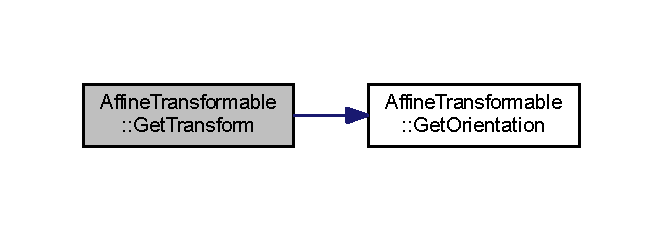
\includegraphics[width=318pt]{class_affine_transformable_a3eb990ab0b75ad30d3bb667e437d8606_cgraph}
\end{center}
\end{figure}




Here is the caller graph for this function\+:
\nopagebreak
\begin{figure}[H]
\begin{center}
\leavevmode
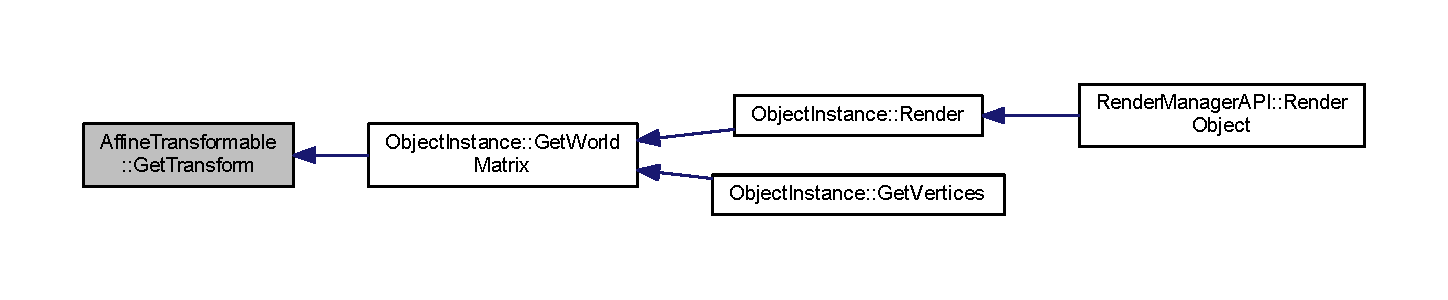
\includegraphics[width=350pt]{class_affine_transformable_a3eb990ab0b75ad30d3bb667e437d8606_icgraph}
\end{center}
\end{figure}


\index{Affine\+Transformable@{Affine\+Transformable}!Get\+Translation@{Get\+Translation}}
\index{Get\+Translation@{Get\+Translation}!Affine\+Transformable@{Affine\+Transformable}}
\subsubsection[{\texorpdfstring{Get\+Translation() const }{GetTranslation() const }}]{\setlength{\rightskip}{0pt plus 5cm}{\bf vec3} const \& Affine\+Transformable\+::\+Get\+Translation (
\begin{DoxyParamCaption}
{}
\end{DoxyParamCaption}
) const}\hypertarget{class_affine_transformable_a6c6a849bb0dc120cdb96494aa40c6898}{}\label{class_affine_transformable_a6c6a849bb0dc120cdb96494aa40c6898}


Gets the translation. 

\begin{DoxyReturn}{Returns}
vec3
\end{DoxyReturn}


Definition at line 19 of file Affine\+Transformable.\+cpp.



References m\+\_\+translation.



Referenced by M\+Camera\+::\+Get\+Position(), and Object\+Instance\+A\+P\+I\+::\+Get\+Translation().


\begin{DoxyCode}
20 \{
21   \textcolor{keywordflow}{return} \hyperlink{class_affine_transformable_a3573983127e380c3d9151c32b43d199d}{m\_translation};
22 \}
\end{DoxyCode}


Here is the caller graph for this function\+:\nopagebreak
\begin{figure}[H]
\begin{center}
\leavevmode
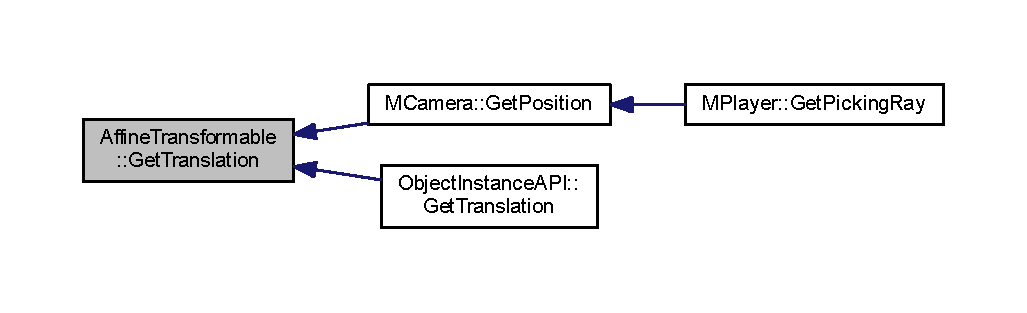
\includegraphics[width=350pt]{class_affine_transformable_a6c6a849bb0dc120cdb96494aa40c6898_icgraph}
\end{center}
\end{figure}


\index{Affine\+Transformable@{Affine\+Transformable}!Get\+Yaw@{Get\+Yaw}}
\index{Get\+Yaw@{Get\+Yaw}!Affine\+Transformable@{Affine\+Transformable}}
\subsubsection[{\texorpdfstring{Get\+Yaw() const }{GetYaw() const }}]{\setlength{\rightskip}{0pt plus 5cm}float Affine\+Transformable\+::\+Get\+Yaw (
\begin{DoxyParamCaption}
{}
\end{DoxyParamCaption}
) const}\hypertarget{class_affine_transformable_afcc35bdd6301a92f87d339f386743d93}{}\label{class_affine_transformable_afcc35bdd6301a92f87d339f386743d93}


Gets the yaw. 

\begin{DoxyReturn}{Returns}
float
\end{DoxyReturn}


Definition at line 46 of file Affine\+Transformable.\+cpp.



References m\+\_\+yaw.


\begin{DoxyCode}
47 \{
48   \textcolor{keywordflow}{return} \hyperlink{_m_math_8h_a8a41524e2041d1382fe880bedddd20a1}{RadToDeg}(\hyperlink{class_affine_transformable_abf9b231dc1bd3e61bbbed8714f127f93}{m\_yaw});
49 \}
\end{DoxyCode}
\index{Affine\+Transformable@{Affine\+Transformable}!Set\+Orientation@{Set\+Orientation}}
\index{Set\+Orientation@{Set\+Orientation}!Affine\+Transformable@{Affine\+Transformable}}
\subsubsection[{\texorpdfstring{Set\+Orientation(float deg\+Yaw, float deg\+Pitch, float deg\+Roll)}{SetOrientation(float degYaw, float degPitch, float degRoll)}}]{\setlength{\rightskip}{0pt plus 5cm}void Affine\+Transformable\+::\+Set\+Orientation (
\begin{DoxyParamCaption}
\item[{float}]{deg\+Yaw, }
\item[{float}]{deg\+Pitch, }
\item[{float}]{deg\+Roll}
\end{DoxyParamCaption}
)}\hypertarget{class_affine_transformable_a9565967f58321117e198b6925c4200d6}{}\label{class_affine_transformable_a9565967f58321117e198b6925c4200d6}


Sets the orientation. 


\begin{DoxyParams}{Parameters}
{\em deg\+Yaw} & The yaw in degrees.\\
\hline
{\em deg\+Pitch} & The pitch in degrees.\\
\hline
{\em deg\+Roll} & The roll in degrees.\\
\hline
\end{DoxyParams}


Definition at line 39 of file Affine\+Transformable.\+cpp.



References Set\+Pitch(), Set\+Roll(), and Set\+Yaw().



Referenced by Affine\+Transformable(), Object\+Instance\+A\+P\+I\+::\+Set\+Orientation(), and Set\+Transform().


\begin{DoxyCode}
40 \{
41   \hyperlink{class_affine_transformable_a47ab5b07df1ee77ae2e63dc0804c5caa}{SetYaw}(yaw);
42   \hyperlink{class_affine_transformable_a8413b02e25aec2a759d5fd269d13fc02}{SetPitch}(pitch);
43   \hyperlink{class_affine_transformable_a9db54f563d9db087b43b64a371200264}{SetRoll}(roll);
44 \}
\end{DoxyCode}


Here is the call graph for this function\+:\nopagebreak
\begin{figure}[H]
\begin{center}
\leavevmode
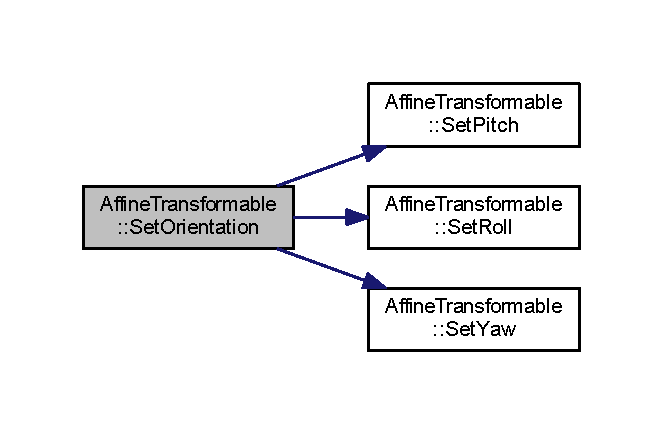
\includegraphics[width=318pt]{class_affine_transformable_a9565967f58321117e198b6925c4200d6_cgraph}
\end{center}
\end{figure}




Here is the caller graph for this function\+:\nopagebreak
\begin{figure}[H]
\begin{center}
\leavevmode
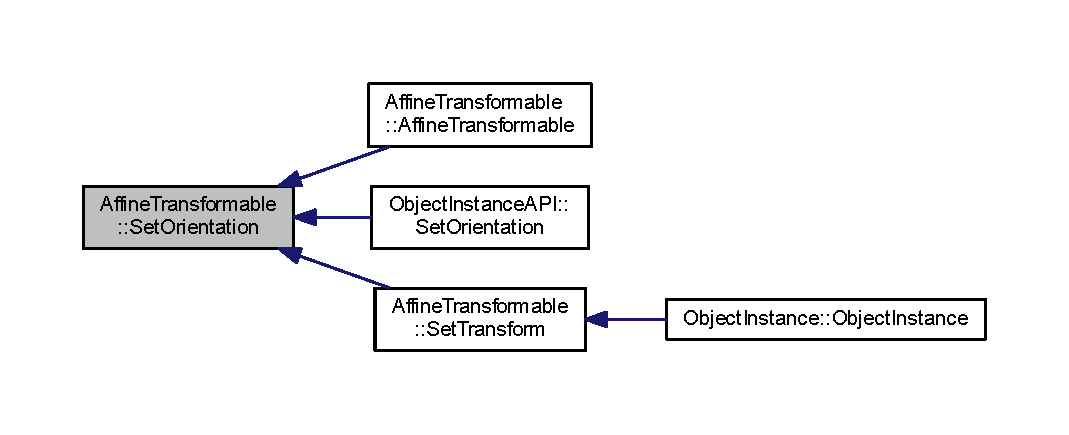
\includegraphics[width=350pt]{class_affine_transformable_a9565967f58321117e198b6925c4200d6_icgraph}
\end{center}
\end{figure}


\index{Affine\+Transformable@{Affine\+Transformable}!Set\+Pitch@{Set\+Pitch}}
\index{Set\+Pitch@{Set\+Pitch}!Affine\+Transformable@{Affine\+Transformable}}
\subsubsection[{\texorpdfstring{Set\+Pitch(float deg\+Pitch)}{SetPitch(float degPitch)}}]{\setlength{\rightskip}{0pt plus 5cm}void Affine\+Transformable\+::\+Set\+Pitch (
\begin{DoxyParamCaption}
\item[{float}]{deg\+Pitch}
\end{DoxyParamCaption}
)}\hypertarget{class_affine_transformable_a8413b02e25aec2a759d5fd269d13fc02}{}\label{class_affine_transformable_a8413b02e25aec2a759d5fd269d13fc02}


Sets the pitch. 


\begin{DoxyParams}{Parameters}
{\em deg\+Pitch} & The pitch in degrees.\\
\hline
\end{DoxyParams}


Definition at line 61 of file Affine\+Transformable.\+cpp.



References m\+\_\+pitch.



Referenced by Set\+Orientation(), and Object\+Instance\+A\+P\+I\+::\+Set\+Rotation().


\begin{DoxyCode}
62 \{
63   \hyperlink{class_affine_transformable_ade24cef424ce102502357cde8214d54b}{m\_pitch} = \hyperlink{_m_math_8h_a12596bd7bfb634efa54d7493e6d546a8}{DegToRad}(pitch);
64 \}
\end{DoxyCode}


Here is the caller graph for this function\+:\nopagebreak
\begin{figure}[H]
\begin{center}
\leavevmode
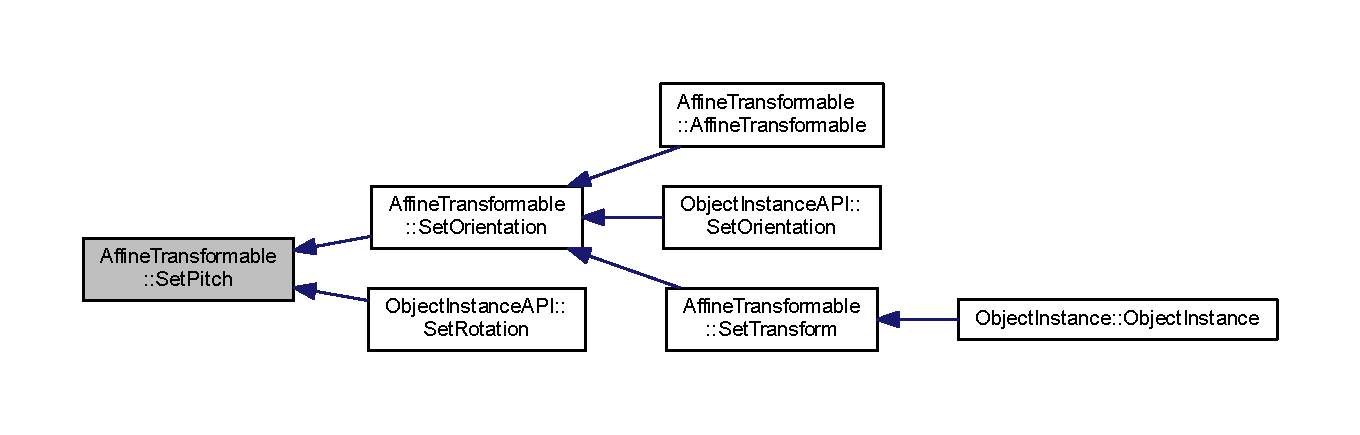
\includegraphics[width=350pt]{class_affine_transformable_a8413b02e25aec2a759d5fd269d13fc02_icgraph}
\end{center}
\end{figure}


\index{Affine\+Transformable@{Affine\+Transformable}!Set\+Roll@{Set\+Roll}}
\index{Set\+Roll@{Set\+Roll}!Affine\+Transformable@{Affine\+Transformable}}
\subsubsection[{\texorpdfstring{Set\+Roll(float deg\+Roll)}{SetRoll(float degRoll)}}]{\setlength{\rightskip}{0pt plus 5cm}void Affine\+Transformable\+::\+Set\+Roll (
\begin{DoxyParamCaption}
\item[{float}]{deg\+Roll}
\end{DoxyParamCaption}
)}\hypertarget{class_affine_transformable_a9db54f563d9db087b43b64a371200264}{}\label{class_affine_transformable_a9db54f563d9db087b43b64a371200264}


Sets the roll. 


\begin{DoxyParams}{Parameters}
{\em deg\+Roll} & The deg roll.\\
\hline
\end{DoxyParams}


Definition at line 71 of file Affine\+Transformable.\+cpp.



References m\+\_\+roll.



Referenced by Set\+Orientation(), and Object\+Instance\+A\+P\+I\+::\+Set\+Rotation().


\begin{DoxyCode}
72 \{
73   \hyperlink{class_affine_transformable_a33e3fc9a32cafaa0a04c6058f283d437}{m\_roll} = \hyperlink{_m_math_8h_a12596bd7bfb634efa54d7493e6d546a8}{DegToRad}(roll);
74 \}
\end{DoxyCode}


Here is the caller graph for this function\+:\nopagebreak
\begin{figure}[H]
\begin{center}
\leavevmode
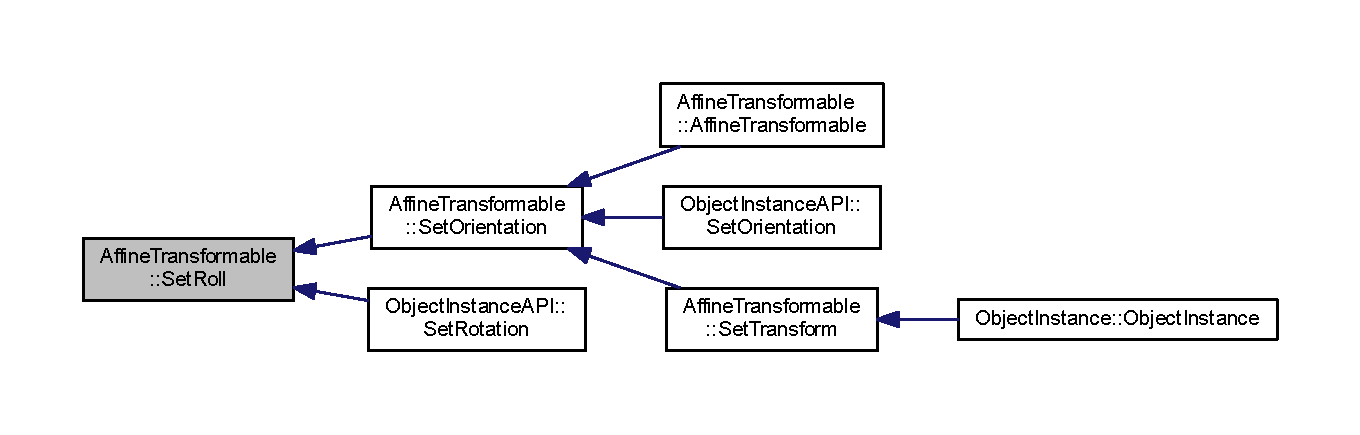
\includegraphics[width=350pt]{class_affine_transformable_a9db54f563d9db087b43b64a371200264_icgraph}
\end{center}
\end{figure}


\index{Affine\+Transformable@{Affine\+Transformable}!Set\+Scale@{Set\+Scale}}
\index{Set\+Scale@{Set\+Scale}!Affine\+Transformable@{Affine\+Transformable}}
\subsubsection[{\texorpdfstring{Set\+Scale(vec3 const \&scale)}{SetScale(vec3 const &scale)}}]{\setlength{\rightskip}{0pt plus 5cm}void Affine\+Transformable\+::\+Set\+Scale (
\begin{DoxyParamCaption}
\item[{{\bf vec3} const \&}]{scale}
\end{DoxyParamCaption}
)}\hypertarget{class_affine_transformable_a215383be79781d61103dfdf8c201be22}{}\label{class_affine_transformable_a215383be79781d61103dfdf8c201be22}


Sets the scale. 


\begin{DoxyParams}{Parameters}
{\em scale} & The scale.\\
\hline
\end{DoxyParams}


Definition at line 81 of file Affine\+Transformable.\+cpp.



References m\+\_\+scale.



Referenced by Affine\+Transformable(), and Set\+Transform().


\begin{DoxyCode}
82 \{
83   \hyperlink{class_affine_transformable_ac332af15336f089337fd31d7b3996bad}{m\_scale} = scale;
84 \}
\end{DoxyCode}


Here is the caller graph for this function\+:\nopagebreak
\begin{figure}[H]
\begin{center}
\leavevmode
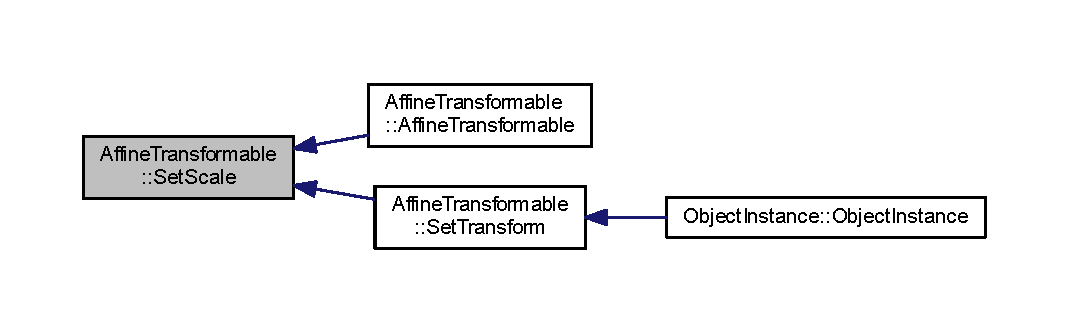
\includegraphics[width=350pt]{class_affine_transformable_a215383be79781d61103dfdf8c201be22_icgraph}
\end{center}
\end{figure}


\index{Affine\+Transformable@{Affine\+Transformable}!Set\+Transform@{Set\+Transform}}
\index{Set\+Transform@{Set\+Transform}!Affine\+Transformable@{Affine\+Transformable}}
\subsubsection[{\texorpdfstring{Set\+Transform(mat4 const \&transform)}{SetTransform(mat4 const &transform)}}]{\setlength{\rightskip}{0pt plus 5cm}void Affine\+Transformable\+::\+Set\+Transform (
\begin{DoxyParamCaption}
\item[{{\bf mat4} const \&}]{transform}
\end{DoxyParamCaption}
)}\hypertarget{class_affine_transformable_aacc67804c045aa75da888ca3ea409939}{}\label{class_affine_transformable_aacc67804c045aa75da888ca3ea409939}


Sets the transform. 


\begin{DoxyParams}{Parameters}
{\em transform} & The transform.\\
\hline
\end{DoxyParams}


Definition at line 94 of file Affine\+Transformable.\+cpp.


\begin{DoxyCode}
95 \{
96   \hyperlink{_types_8h_a02abcac728eae225e929e9e0dc427f28}{quat} temp;
97   \hyperlink{_types_8h_a3d0ce73e3199de81565fb01632415288}{vec3} skew;
98   \hyperlink{_types_8h_ac54e849f8b2339f592307eaf6cdbba77}{vec4} perspective;
99   glm::decompose(transform, \hyperlink{class_affine_transformable_ac332af15336f089337fd31d7b3996bad}{m\_scale}, temp, \hyperlink{class_affine_transformable_a3573983127e380c3d9151c32b43d199d}{m\_translation}, skew, perspective);
100 
101   \hyperlink{_types_8h_a3d0ce73e3199de81565fb01632415288}{vec3} eulers = \hyperlink{_m_math_8h_a8a41524e2041d1382fe880bedddd20a1}{RadToDeg}(eulerAngles(temp));
102   \hyperlink{class_affine_transformable_a9565967f58321117e198b6925c4200d6}{SetOrientation}(eulers.y, eulers.x, eulers.z);
103 \}
\end{DoxyCode}
\index{Affine\+Transformable@{Affine\+Transformable}!Set\+Transform@{Set\+Transform}}
\index{Set\+Transform@{Set\+Transform}!Affine\+Transformable@{Affine\+Transformable}}
\subsubsection[{\texorpdfstring{Set\+Transform(vec3 const \&translation, float yaw, float pitch, float roll, vec3 const \&scale)}{SetTransform(vec3 const &translation, float yaw, float pitch, float roll, vec3 const &scale)}}]{\setlength{\rightskip}{0pt plus 5cm}void Affine\+Transformable\+::\+Set\+Transform (
\begin{DoxyParamCaption}
\item[{{\bf vec3} const \&}]{translation, }
\item[{float}]{yaw, }
\item[{float}]{pitch, }
\item[{float}]{roll, }
\item[{{\bf vec3} const \&}]{scale}
\end{DoxyParamCaption}
)}\hypertarget{class_affine_transformable_ac4faa6d4c8127e61622ae265ba708276}{}\label{class_affine_transformable_ac4faa6d4c8127e61622ae265ba708276}


Sets the transform. 


\begin{DoxyParams}{Parameters}
{\em translation} & The translation.\\
\hline
{\em yaw} & The yaw.\\
\hline
{\em pitch} & The pitch.\\
\hline
{\em roll} & The roll.\\
\hline
{\em scale} & The scale.\\
\hline
\end{DoxyParams}


Definition at line 105 of file Affine\+Transformable.\+cpp.



References Set\+Orientation(), Set\+Scale(), and Set\+Translation().



Referenced by Object\+Instance\+::\+Object\+Instance().


\begin{DoxyCode}
106 \{
107   \hyperlink{class_affine_transformable_abd554f0c81205675ed2a6520e09e5b98}{SetTranslation}(translation);
108   \hyperlink{class_affine_transformable_a9565967f58321117e198b6925c4200d6}{SetOrientation}(yaw, pitch, roll);
109   \hyperlink{class_affine_transformable_a215383be79781d61103dfdf8c201be22}{SetScale}(scale);
110 \}
\end{DoxyCode}


Here is the call graph for this function\+:\nopagebreak
\begin{figure}[H]
\begin{center}
\leavevmode
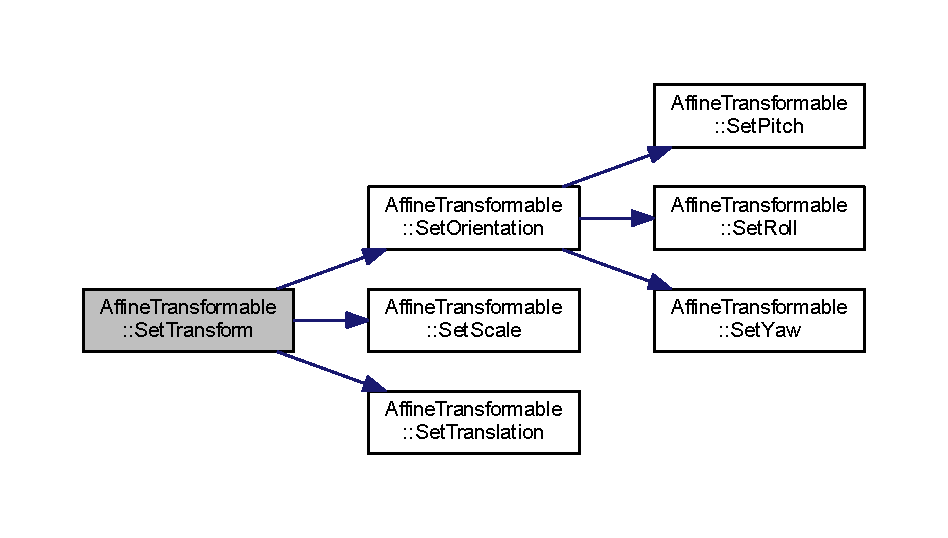
\includegraphics[width=350pt]{class_affine_transformable_ac4faa6d4c8127e61622ae265ba708276_cgraph}
\end{center}
\end{figure}




Here is the caller graph for this function\+:\nopagebreak
\begin{figure}[H]
\begin{center}
\leavevmode
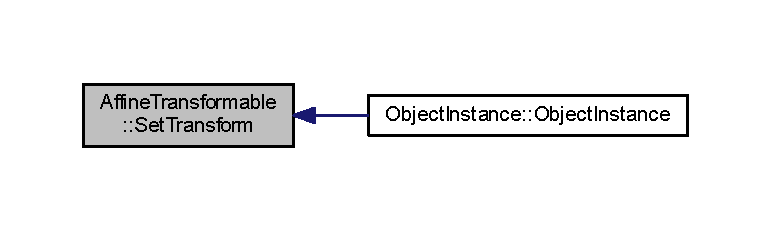
\includegraphics[width=350pt]{class_affine_transformable_ac4faa6d4c8127e61622ae265ba708276_icgraph}
\end{center}
\end{figure}


\index{Affine\+Transformable@{Affine\+Transformable}!Set\+Translation@{Set\+Translation}}
\index{Set\+Translation@{Set\+Translation}!Affine\+Transformable@{Affine\+Transformable}}
\subsubsection[{\texorpdfstring{Set\+Translation(vec3 const \&translation)}{SetTranslation(vec3 const &translation)}}]{\setlength{\rightskip}{0pt plus 5cm}void Affine\+Transformable\+::\+Set\+Translation (
\begin{DoxyParamCaption}
\item[{{\bf vec3} const \&}]{translation}
\end{DoxyParamCaption}
)}\hypertarget{class_affine_transformable_abd554f0c81205675ed2a6520e09e5b98}{}\label{class_affine_transformable_abd554f0c81205675ed2a6520e09e5b98}


Sets the translation. 


\begin{DoxyParams}{Parameters}
{\em translation} & The translation.\\
\hline
\end{DoxyParams}


Definition at line 24 of file Affine\+Transformable.\+cpp.



References m\+\_\+translation.



Referenced by Affine\+Transformable(), M\+Camera\+::\+Set\+Position(), and Set\+Transform().


\begin{DoxyCode}
25 \{
26   \hyperlink{class_affine_transformable_a3573983127e380c3d9151c32b43d199d}{m\_translation} = translation;
27 \}
\end{DoxyCode}


Here is the caller graph for this function\+:\nopagebreak
\begin{figure}[H]
\begin{center}
\leavevmode
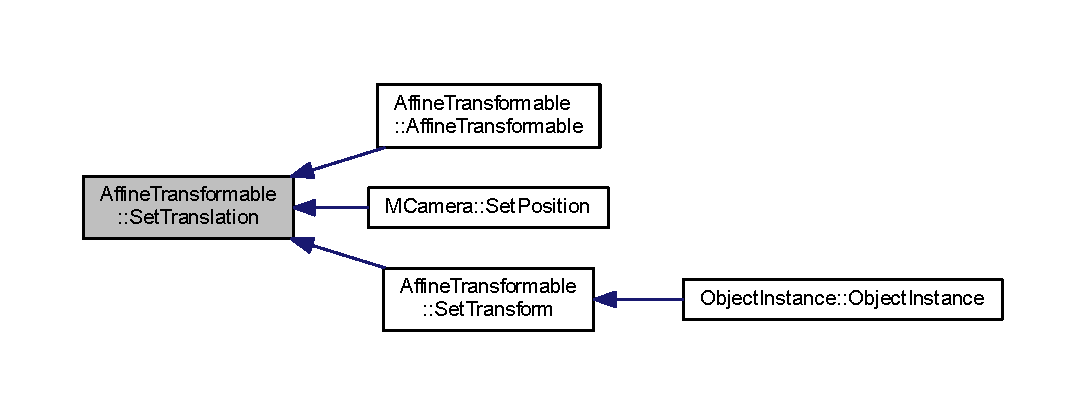
\includegraphics[width=350pt]{class_affine_transformable_abd554f0c81205675ed2a6520e09e5b98_icgraph}
\end{center}
\end{figure}


\index{Affine\+Transformable@{Affine\+Transformable}!Set\+Translation@{Set\+Translation}}
\index{Set\+Translation@{Set\+Translation}!Affine\+Transformable@{Affine\+Transformable}}
\subsubsection[{\texorpdfstring{Set\+Translation(float x, float y, float z)}{SetTranslation(float x, float y, float z)}}]{\setlength{\rightskip}{0pt plus 5cm}void Affine\+Transformable\+::\+Set\+Translation (
\begin{DoxyParamCaption}
\item[{float}]{x, }
\item[{float}]{y, }
\item[{float}]{z}
\end{DoxyParamCaption}
)}\hypertarget{class_affine_transformable_a47eccc886862946587d6e9de46f55dff}{}\label{class_affine_transformable_a47eccc886862946587d6e9de46f55dff}


Sets the translation. 


\begin{DoxyParams}{Parameters}
{\em x} & The x.\\
\hline
{\em y} & The y.\\
\hline
{\em z} & The z.\\
\hline
\end{DoxyParams}


Definition at line 29 of file Affine\+Transformable.\+cpp.


\begin{DoxyCode}
30 \{
31   \hyperlink{class_affine_transformable_abd554f0c81205675ed2a6520e09e5b98}{SetTranslation}(\hyperlink{_types_8h_a3d0ce73e3199de81565fb01632415288}{vec3}\{ x, y, z \});
32 \}
\end{DoxyCode}
\index{Affine\+Transformable@{Affine\+Transformable}!Set\+Yaw@{Set\+Yaw}}
\index{Set\+Yaw@{Set\+Yaw}!Affine\+Transformable@{Affine\+Transformable}}
\subsubsection[{\texorpdfstring{Set\+Yaw(float deg\+Yaw)}{SetYaw(float degYaw)}}]{\setlength{\rightskip}{0pt plus 5cm}void Affine\+Transformable\+::\+Set\+Yaw (
\begin{DoxyParamCaption}
\item[{float}]{deg\+Yaw}
\end{DoxyParamCaption}
)}\hypertarget{class_affine_transformable_a47ab5b07df1ee77ae2e63dc0804c5caa}{}\label{class_affine_transformable_a47ab5b07df1ee77ae2e63dc0804c5caa}


Sets the yaw. 


\begin{DoxyParams}{Parameters}
{\em deg\+Yaw} & The yaw in degrees.\\
\hline
\end{DoxyParams}


Definition at line 51 of file Affine\+Transformable.\+cpp.



References m\+\_\+yaw.



Referenced by Forest\+Terrain\+::\+Generate\+Forest(), Set\+Orientation(), and Object\+Instance\+A\+P\+I\+::\+Set\+Rotation().


\begin{DoxyCode}
52 \{
53   \hyperlink{class_affine_transformable_abf9b231dc1bd3e61bbbed8714f127f93}{m\_yaw} = \hyperlink{_m_math_8h_a12596bd7bfb634efa54d7493e6d546a8}{DegToRad}(yaw);
54 \}
\end{DoxyCode}


Here is the caller graph for this function\+:
\nopagebreak
\begin{figure}[H]
\begin{center}
\leavevmode
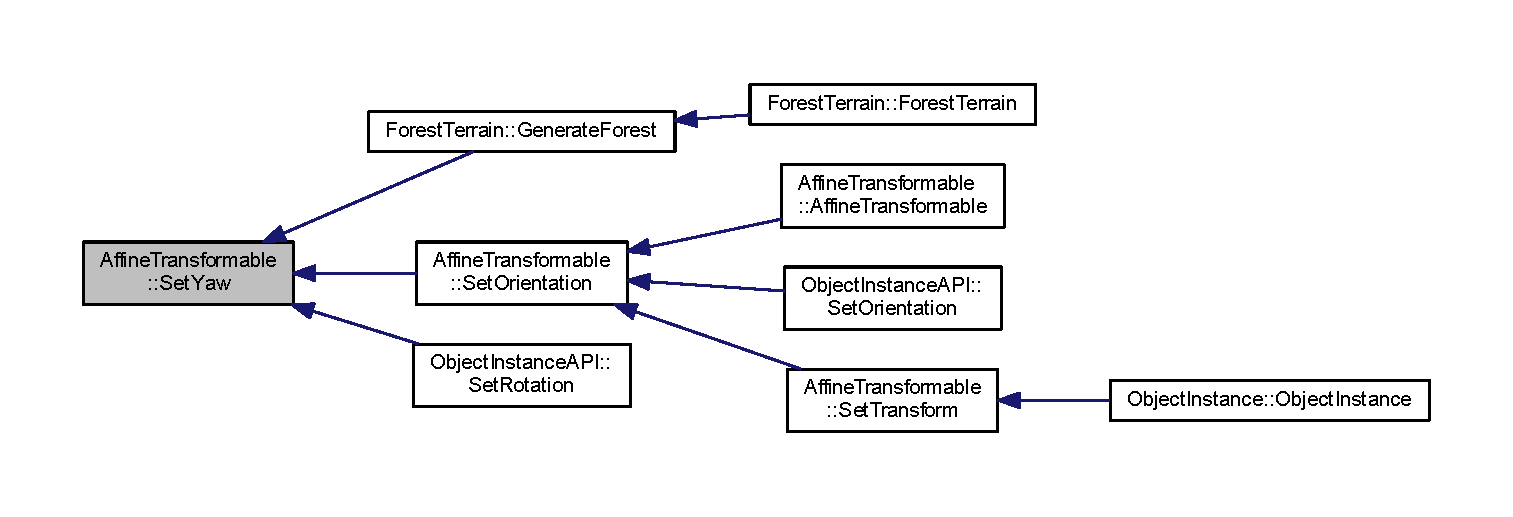
\includegraphics[width=350pt]{class_affine_transformable_a47ab5b07df1ee77ae2e63dc0804c5caa_icgraph}
\end{center}
\end{figure}




\subsection{Member Data Documentation}
\index{Affine\+Transformable@{Affine\+Transformable}!m\+\_\+pitch@{m\+\_\+pitch}}
\index{m\+\_\+pitch@{m\+\_\+pitch}!Affine\+Transformable@{Affine\+Transformable}}
\subsubsection[{\texorpdfstring{m\+\_\+pitch}{m_pitch}}]{\setlength{\rightskip}{0pt plus 5cm}float Affine\+Transformable\+::m\+\_\+pitch\hspace{0.3cm}{\ttfamily [private]}}\hypertarget{class_affine_transformable_ade24cef424ce102502357cde8214d54b}{}\label{class_affine_transformable_ade24cef424ce102502357cde8214d54b}


The pitch 



Definition at line 33 of file Affine\+Transformable.\+h.



Referenced by Get\+Pitch(), and Set\+Pitch().

\index{Affine\+Transformable@{Affine\+Transformable}!m\+\_\+roll@{m\+\_\+roll}}
\index{m\+\_\+roll@{m\+\_\+roll}!Affine\+Transformable@{Affine\+Transformable}}
\subsubsection[{\texorpdfstring{m\+\_\+roll}{m_roll}}]{\setlength{\rightskip}{0pt plus 5cm}float Affine\+Transformable\+::m\+\_\+roll\hspace{0.3cm}{\ttfamily [private]}}\hypertarget{class_affine_transformable_a33e3fc9a32cafaa0a04c6058f283d437}{}\label{class_affine_transformable_a33e3fc9a32cafaa0a04c6058f283d437}


The roll 



Definition at line 38 of file Affine\+Transformable.\+h.



Referenced by Get\+Roll(), and Set\+Roll().

\index{Affine\+Transformable@{Affine\+Transformable}!m\+\_\+scale@{m\+\_\+scale}}
\index{m\+\_\+scale@{m\+\_\+scale}!Affine\+Transformable@{Affine\+Transformable}}
\subsubsection[{\texorpdfstring{m\+\_\+scale}{m_scale}}]{\setlength{\rightskip}{0pt plus 5cm}{\bf vec3} Affine\+Transformable\+::m\+\_\+scale\hspace{0.3cm}{\ttfamily [private]}}\hypertarget{class_affine_transformable_ac332af15336f089337fd31d7b3996bad}{}\label{class_affine_transformable_ac332af15336f089337fd31d7b3996bad}


The scale 



Definition at line 43 of file Affine\+Transformable.\+h.



Referenced by Get\+Scale(), and Set\+Scale().

\index{Affine\+Transformable@{Affine\+Transformable}!m\+\_\+translation@{m\+\_\+translation}}
\index{m\+\_\+translation@{m\+\_\+translation}!Affine\+Transformable@{Affine\+Transformable}}
\subsubsection[{\texorpdfstring{m\+\_\+translation}{m_translation}}]{\setlength{\rightskip}{0pt plus 5cm}{\bf vec3} Affine\+Transformable\+::m\+\_\+translation\hspace{0.3cm}{\ttfamily [private]}}\hypertarget{class_affine_transformable_a3573983127e380c3d9151c32b43d199d}{}\label{class_affine_transformable_a3573983127e380c3d9151c32b43d199d}


The translation 



Definition at line 23 of file Affine\+Transformable.\+h.



Referenced by Affine\+Transformable(), Get\+Translation(), and Set\+Translation().

\index{Affine\+Transformable@{Affine\+Transformable}!m\+\_\+yaw@{m\+\_\+yaw}}
\index{m\+\_\+yaw@{m\+\_\+yaw}!Affine\+Transformable@{Affine\+Transformable}}
\subsubsection[{\texorpdfstring{m\+\_\+yaw}{m_yaw}}]{\setlength{\rightskip}{0pt plus 5cm}float Affine\+Transformable\+::m\+\_\+yaw\hspace{0.3cm}{\ttfamily [private]}}\hypertarget{class_affine_transformable_abf9b231dc1bd3e61bbbed8714f127f93}{}\label{class_affine_transformable_abf9b231dc1bd3e61bbbed8714f127f93}


The yaw 



Definition at line 28 of file Affine\+Transformable.\+h.



Referenced by Get\+Yaw(), and Set\+Yaw().



The documentation for this class was generated from the following files\+:\begin{DoxyCompactItemize}
\item 
C\+:/\+Users/elizabeth/\+Documents/\+Git\+Hub/\+Engine/\+Open\+G\+L\+Engine/\+Open\+G\+L\+Engine/\hyperlink{_affine_transformable_8h}{Affine\+Transformable.\+h}\item 
C\+:/\+Users/elizabeth/\+Documents/\+Git\+Hub/\+Engine/\+Open\+G\+L\+Engine/\+Open\+G\+L\+Engine/\hyperlink{_affine_transformable_8cpp}{Affine\+Transformable.\+cpp}\end{DoxyCompactItemize}

\hypertarget{struct_agent}{}\section{Agent Struct Reference}
\label{struct_agent}\index{Agent@{Agent}}


{\ttfamily \#include $<$Agent.\+h$>$}



Collaboration diagram for Agent\+:\nopagebreak
\begin{figure}[H]
\begin{center}
\leavevmode
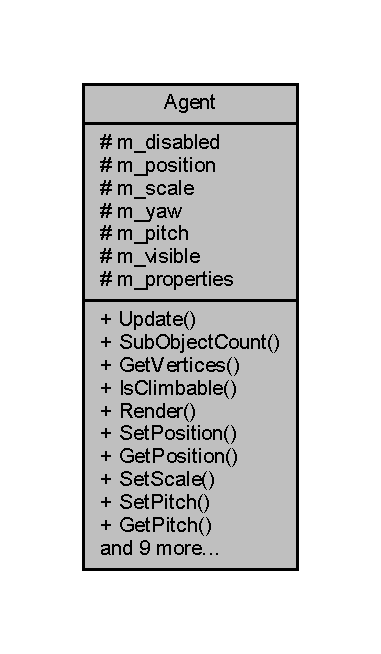
\includegraphics[width=183pt]{struct_agent__coll__graph}
\end{center}
\end{figure}
\subsection*{Public Member Functions}
\begin{DoxyCompactItemize}
\item 
virtual void \hyperlink{struct_agent_a511d2a3f9962d7b8b8ed8e55bb2fd9b2}{Update} ()=0
\begin{DoxyCompactList}\small\item\em Calls the supplied update function if it has been implemented. \end{DoxyCompactList}\item 
virtual int \hyperlink{struct_agent_a1088932d3e1dcce8ff7ee49a5ab64f57}{Sub\+Object\+Count} ()=0
\begin{DoxyCompactList}\small\item\em Returns the number of sub-\/objects in the model rendered with a different material. \end{DoxyCompactList}\item 
virtual std\+::vector$<$ \hyperlink{_types_8h_a3d0ce73e3199de81565fb01632415288}{glm\+::vec3} $>$ \hyperlink{struct_agent_a98530102fcae3e3ed6e97102efbfdf38}{Get\+Vertices} (int sub\+Index, \hyperlink{_types_8h_a2db59f395fe82a7394c6324956c265d8}{glm\+::mat4} parent\+Model\+Matrix=\hyperlink{_types_8h_a2db59f395fe82a7394c6324956c265d8}{glm\+::mat4}())=0
\begin{DoxyCompactList}\small\item\em Returns a vector of vertices for the specified sub object. \end{DoxyCompactList}\item 
virtual bool \hyperlink{struct_agent_a6eef7edaf0c490be38ac5b9fa4a88754}{Is\+Climbable} (int sub\+Index)=0
\begin{DoxyCompactList}\small\item\em Returns the climbability of the sub-\/object. \end{DoxyCompactList}\item 
virtual void \hyperlink{struct_agent_a7f9cd5a90b4766b24f49e5100cfe5026}{Render} (\hyperlink{_types_8h_a2db59f395fe82a7394c6324956c265d8}{glm\+::mat4} view\+Matrix, \hyperlink{_types_8h_a2db59f395fe82a7394c6324956c265d8}{glm\+::mat4} projection\+Matrix, \hyperlink{_types_8h_a2db59f395fe82a7394c6324956c265d8}{glm\+::mat4} parent\+Model\+Matrix=\hyperlink{_types_8h_a2db59f395fe82a7394c6324956c265d8}{glm\+::mat4}())=0
\begin{DoxyCompactList}\small\item\em Render an object. \end{DoxyCompactList}\item 
void \hyperlink{struct_agent_a0502dba36dde5b51033e38c744f2db11}{Set\+Position} (\hyperlink{_types_8h_a3d0ce73e3199de81565fb01632415288}{glm\+::vec3} coords)
\begin{DoxyCompactList}\small\item\em Sets the position that the model will be rendered at in the world. \end{DoxyCompactList}\item 
\hyperlink{_types_8h_a3d0ce73e3199de81565fb01632415288}{vec3} \hyperlink{struct_agent_a7f42342662f587ec076b7f283000331a}{Get\+Position} ()
\begin{DoxyCompactList}\small\item\em Get the posistion of the agent. \end{DoxyCompactList}\item 
void \hyperlink{struct_agent_afaba4f5661ada2bec70aee15e71852bd}{Set\+Scale} (\hyperlink{_types_8h_a3d0ce73e3199de81565fb01632415288}{glm\+::vec3} a\+\_\+scale)
\begin{DoxyCompactList}\small\item\em Sets the scale that the model will be rendered at in the world. \end{DoxyCompactList}\item 
void \hyperlink{struct_agent_a4ac318bdc2653ecbbbe95ab74602e207}{Set\+Pitch} (float degrees)
\begin{DoxyCompactList}\small\item\em Rotates the model by a specified number of degrees around the x-\/axis. \end{DoxyCompactList}\item 
float \hyperlink{struct_agent_a0ba5a593c61ffb2c199766478fe24af7}{Get\+Pitch} ()
\begin{DoxyCompactList}\small\item\em Gets the pitch. \end{DoxyCompactList}\item 
void \hyperlink{struct_agent_aa3295f1b269d653a36cb63aae7587576}{Set\+Yaw} (float degrees)
\begin{DoxyCompactList}\small\item\em Rotates the model by a specified number of degrees around the y-\/axis. \end{DoxyCompactList}\item 
float \hyperlink{struct_agent_ab8fd6738035a240f0a5cf77d9904b5f7}{Get\+Yaw} ()
\begin{DoxyCompactList}\small\item\em Gets the yaw. \end{DoxyCompactList}\item 
void \hyperlink{struct_agent_a82766fa6b32f2f347c79eb669dd080d6}{Set\+Visible} (bool b)
\begin{DoxyCompactList}\small\item\em Determines whether or not the object is visible. \end{DoxyCompactList}\item 
bool \hyperlink{struct_agent_a5be15897c8663390f65c18d59c8dd883}{Get\+Visible} ()
\begin{DoxyCompactList}\small\item\em Returns true if the object is visible, false if the object is invisible. \end{DoxyCompactList}\item 
\hyperlink{_types_8h_a2db59f395fe82a7394c6324956c265d8}{glm\+::mat4} \hyperlink{struct_agent_a3b0f5c28eddeda3fcf002633ab43fae0}{Get\+Model\+Matrix} ()
\begin{DoxyCompactList}\small\item\em Gets the model matrix. \end{DoxyCompactList}\item 
bool \hyperlink{struct_agent_a51d3f034af5810302abb3eda96d66d39}{Check\+Property} (\hyperlink{_agent_8h_ab486bd3cbb07abc600b5b7586f95f7f5}{Agent\+Property} target)
\begin{DoxyCompactList}\small\item\em Get the value (true/false) of a specified Agent\+Property. \end{DoxyCompactList}\item 
void \hyperlink{struct_agent_ae9dba04d6c1ca72bb6451f1f2f81be95}{Set\+Property} (\hyperlink{_agent_8h_ab486bd3cbb07abc600b5b7586f95f7f5}{Agent\+Property} prop, bool value)
\begin{DoxyCompactList}\small\item\em Set the value (true/false) of a specified Agent\+Property. \end{DoxyCompactList}\item 
void \hyperlink{struct_agent_a01fb711b44cb03494a9751f66a7b4d7e}{Set\+Disabled} (bool new\+Dis)
\begin{DoxyCompactList}\small\item\em set the value for disabled \end{DoxyCompactList}\item 
bool \hyperlink{struct_agent_a29b7642fb4e6e623700ab479561fcdfb}{Get\+Disabled} ()
\begin{DoxyCompactList}\small\item\em Get the value for disabled. \end{DoxyCompactList}\end{DoxyCompactItemize}
\subsection*{Protected Attributes}
\begin{DoxyCompactItemize}
\item 
bool \hyperlink{struct_agent_aa0d2f2202888755e79f3d8022e79d816}{m\+\_\+disabled} = false
\begin{DoxyCompactList}\small\item\em disabled -\/ whether the agent is disabled \end{DoxyCompactList}\item 
\hyperlink{_types_8h_a3d0ce73e3199de81565fb01632415288}{glm\+::vec3} \hyperlink{struct_agent_aba44b4b1781713d1ec074b079c5dc4e1}{m\+\_\+position}
\begin{DoxyCompactList}\small\item\em posistion -\/ the coordinates of the agent \end{DoxyCompactList}\item 
\hyperlink{_types_8h_a3d0ce73e3199de81565fb01632415288}{glm\+::vec3} \hyperlink{struct_agent_abc8afe26ba8fbe75eba18ee7ccf45c7e}{m\+\_\+scale}
\begin{DoxyCompactList}\small\item\em scale -\/ the scale of the agent \end{DoxyCompactList}\item 
float \hyperlink{struct_agent_ab247e82de72e83d05afea649311a9314}{m\+\_\+yaw} = 0
\begin{DoxyCompactList}\small\item\em yaw -\/ the yaw of the agent \end{DoxyCompactList}\item 
float \hyperlink{struct_agent_aec2384613e952e3f4e280985743f41ce}{m\+\_\+pitch} = 0
\begin{DoxyCompactList}\small\item\em pitch -\/ the pitch of the agent \end{DoxyCompactList}\item 
bool \hyperlink{struct_agent_a0155e68895c28427071104719d710fc1}{m\+\_\+visible} = true
\begin{DoxyCompactList}\small\item\em visible -\/ whether the agent is visible \end{DoxyCompactList}\item 
\hyperlink{_agent_8h_ab486bd3cbb07abc600b5b7586f95f7f5}{Agent\+Property} \hyperlink{struct_agent_a323d48d9a1fe0b993aad8700e051d4c4}{m\+\_\+properties}
\begin{DoxyCompactList}\small\item\em properties -\/ properties of the agent \end{DoxyCompactList}\end{DoxyCompactItemize}


\subsection{Detailed Description}


Definition at line 38 of file Agent.\+h.



\subsection{Member Function Documentation}
\index{Agent@{Agent}!Check\+Property@{Check\+Property}}
\index{Check\+Property@{Check\+Property}!Agent@{Agent}}
\subsubsection[{\texorpdfstring{Check\+Property(\+Agent\+Property target)}{CheckProperty(AgentProperty target)}}]{\setlength{\rightskip}{0pt plus 5cm}bool Agent\+::\+Check\+Property (
\begin{DoxyParamCaption}
\item[{{\bf Agent\+Property}}]{target}
\end{DoxyParamCaption}
)}\hypertarget{struct_agent_a51d3f034af5810302abb3eda96d66d39}{}\label{struct_agent_a51d3f034af5810302abb3eda96d66d39}


Get the value (true/false) of a specified Agent\+Property. 


\begin{DoxyParams}{Parameters}
{\em target} & -\/ Name of the agent property to check.\\
\hline
\end{DoxyParams}
\begin{DoxyReturn}{Returns}
void 
\end{DoxyReturn}


Definition at line 57 of file Agent.\+cpp.



References m\+\_\+properties.


\begin{DoxyCode}
58 \{
59     \textcolor{keywordflow}{return} (\hyperlink{struct_agent_a323d48d9a1fe0b993aad8700e051d4c4}{m\_properties} & target) != 0;
60 \}
\end{DoxyCode}
\index{Agent@{Agent}!Get\+Disabled@{Get\+Disabled}}
\index{Get\+Disabled@{Get\+Disabled}!Agent@{Agent}}
\subsubsection[{\texorpdfstring{Get\+Disabled()}{GetDisabled()}}]{\setlength{\rightskip}{0pt plus 5cm}bool Agent\+::\+Get\+Disabled (
\begin{DoxyParamCaption}
{}
\end{DoxyParamCaption}
)}\hypertarget{struct_agent_a29b7642fb4e6e623700ab479561fcdfb}{}\label{struct_agent_a29b7642fb4e6e623700ab479561fcdfb}


Get the value for disabled. 

\begin{DoxyReturn}{Returns}
bool 
\end{DoxyReturn}


Definition at line 79 of file Agent.\+cpp.



References m\+\_\+disabled.


\begin{DoxyCode}
79                         \{
80     \textcolor{keywordflow}{return} \hyperlink{struct_agent_aa0d2f2202888755e79f3d8022e79d816}{m\_disabled};
81 \}\end{DoxyCode}
\index{Agent@{Agent}!Get\+Model\+Matrix@{Get\+Model\+Matrix}}
\index{Get\+Model\+Matrix@{Get\+Model\+Matrix}!Agent@{Agent}}
\subsubsection[{\texorpdfstring{Get\+Model\+Matrix()}{GetModelMatrix()}}]{\setlength{\rightskip}{0pt plus 5cm}{\bf glm\+::mat4} Agent\+::\+Get\+Model\+Matrix (
\begin{DoxyParamCaption}
{}
\end{DoxyParamCaption}
)}\hypertarget{struct_agent_a3b0f5c28eddeda3fcf002633ab43fae0}{}\label{struct_agent_a3b0f5c28eddeda3fcf002633ab43fae0}


Gets the model matrix. 

\begin{DoxyReturn}{Returns}
glm\+::mat4 
\end{DoxyReturn}


Definition at line 4 of file Agent.\+cpp.


\begin{DoxyCode}
5 \{
6   \hyperlink{_types_8h_a2db59f395fe82a7394c6324956c265d8}{glm::mat4} scaleMatrix = glm::scale(\hyperlink{struct_agent_abc8afe26ba8fbe75eba18ee7ccf45c7e}{m\_scale});
7   \hyperlink{_types_8h_a2db59f395fe82a7394c6324956c265d8}{glm::mat4} YrotationMatrix = glm::rotate(((\hyperlink{struct_agent_ab247e82de72e83d05afea649311a9314}{m\_yaw})* 3.1416f / 180), 
      \hyperlink{_types_8h_a3d0ce73e3199de81565fb01632415288}{glm::vec3}(0, 1, 0));
8   \hyperlink{_types_8h_a2db59f395fe82a7394c6324956c265d8}{glm::mat4} XrotationMatrix = glm::rotate(((\hyperlink{struct_agent_aec2384613e952e3f4e280985743f41ce}{m\_pitch})* 3.1416f / 180), 
      \hyperlink{_types_8h_a3d0ce73e3199de81565fb01632415288}{glm::vec3}(1, 0, 0));
9   \hyperlink{_types_8h_a2db59f395fe82a7394c6324956c265d8}{glm::mat4} translationMatrix = glm::translate(\hyperlink{struct_agent_aba44b4b1781713d1ec074b079c5dc4e1}{m\_position});
10 
11   \textcolor{comment}{//rotates and THEN translates}
12   \textcolor{keywordflow}{return} translationMatrix * XrotationMatrix * YrotationMatrix * scaleMatrix;
13 \}
\end{DoxyCode}
\index{Agent@{Agent}!Get\+Pitch@{Get\+Pitch}}
\index{Get\+Pitch@{Get\+Pitch}!Agent@{Agent}}
\subsubsection[{\texorpdfstring{Get\+Pitch()}{GetPitch()}}]{\setlength{\rightskip}{0pt plus 5cm}float Agent\+::\+Get\+Pitch (
\begin{DoxyParamCaption}
{}
\end{DoxyParamCaption}
)}\hypertarget{struct_agent_a0ba5a593c61ffb2c199766478fe24af7}{}\label{struct_agent_a0ba5a593c61ffb2c199766478fe24af7}


Gets the pitch. 

\begin{DoxyReturn}{Returns}
float 
\end{DoxyReturn}


Definition at line 30 of file Agent.\+cpp.



References m\+\_\+pitch.


\begin{DoxyCode}
31 \{
32   \textcolor{keywordflow}{return} \hyperlink{struct_agent_aec2384613e952e3f4e280985743f41ce}{m\_pitch};
33 \}
\end{DoxyCode}
\index{Agent@{Agent}!Get\+Position@{Get\+Position}}
\index{Get\+Position@{Get\+Position}!Agent@{Agent}}
\subsubsection[{\texorpdfstring{Get\+Position()}{GetPosition()}}]{\setlength{\rightskip}{0pt plus 5cm}{\bf vec3} Agent\+::\+Get\+Position (
\begin{DoxyParamCaption}
{}
\end{DoxyParamCaption}
)}\hypertarget{struct_agent_a7f42342662f587ec076b7f283000331a}{}\label{struct_agent_a7f42342662f587ec076b7f283000331a}


Get the posistion of the agent. 

\begin{DoxyReturn}{Returns}
vec3 
\end{DoxyReturn}


Definition at line 45 of file Agent.\+cpp.


\begin{DoxyCode}
46 \{
47     \textcolor{keywordflow}{return} \hyperlink{struct_agent_aba44b4b1781713d1ec074b079c5dc4e1}{m\_position};
48 \}
\end{DoxyCode}
\index{Agent@{Agent}!Get\+Vertices@{Get\+Vertices}}
\index{Get\+Vertices@{Get\+Vertices}!Agent@{Agent}}
\subsubsection[{\texorpdfstring{Get\+Vertices(int sub\+Index, glm\+::mat4 parent\+Model\+Matrix=glm\+::mat4())=0}{GetVertices(int subIndex, glm::mat4 parentModelMatrix=glm::mat4())=0}}]{\setlength{\rightskip}{0pt plus 5cm}virtual std\+::vector$<${\bf glm\+::vec3}$>$ Agent\+::\+Get\+Vertices (
\begin{DoxyParamCaption}
\item[{int}]{sub\+Index, }
\item[{{\bf glm\+::mat4}}]{parent\+Model\+Matrix = {\ttfamily {\bf glm\+::mat4}()}}
\end{DoxyParamCaption}
)\hspace{0.3cm}{\ttfamily [pure virtual]}}\hypertarget{struct_agent_a98530102fcae3e3ed6e97102efbfdf38}{}\label{struct_agent_a98530102fcae3e3ed6e97102efbfdf38}


Returns a vector of vertices for the specified sub object. 


\begin{DoxyParams}{Parameters}
{\em sub\+Index} & -\/ the index of the sub object needed \\
\hline
{\em parent\+Model\+Matrix} & -\/ the parent model matrix\\
\hline
\end{DoxyParams}
\begin{DoxyReturn}{Returns}
std\+::vector$<$glm\+::vec3$>$ 
\end{DoxyReturn}
\index{Agent@{Agent}!Get\+Visible@{Get\+Visible}}
\index{Get\+Visible@{Get\+Visible}!Agent@{Agent}}
\subsubsection[{\texorpdfstring{Get\+Visible()}{GetVisible()}}]{\setlength{\rightskip}{0pt plus 5cm}bool Agent\+::\+Get\+Visible (
\begin{DoxyParamCaption}
{}
\end{DoxyParamCaption}
)\hspace{0.3cm}{\ttfamily [inline]}}\hypertarget{struct_agent_a5be15897c8663390f65c18d59c8dd883}{}\label{struct_agent_a5be15897c8663390f65c18d59c8dd883}


Returns true if the object is visible, false if the object is invisible. 

\begin{DoxyReturn}{Returns}
bool 
\end{DoxyReturn}


Definition at line 167 of file Agent.\+h.



References m\+\_\+visible.


\begin{DoxyCode}
167 \{ \textcolor{keywordflow}{return} \hyperlink{struct_agent_a0155e68895c28427071104719d710fc1}{m\_visible}; \}
\end{DoxyCode}
\index{Agent@{Agent}!Get\+Yaw@{Get\+Yaw}}
\index{Get\+Yaw@{Get\+Yaw}!Agent@{Agent}}
\subsubsection[{\texorpdfstring{Get\+Yaw()}{GetYaw()}}]{\setlength{\rightskip}{0pt plus 5cm}float Agent\+::\+Get\+Yaw (
\begin{DoxyParamCaption}
{}
\end{DoxyParamCaption}
)}\hypertarget{struct_agent_ab8fd6738035a240f0a5cf77d9904b5f7}{}\label{struct_agent_ab8fd6738035a240f0a5cf77d9904b5f7}


Gets the yaw. 

\begin{DoxyReturn}{Returns}
float 
\end{DoxyReturn}


Definition at line 20 of file Agent.\+cpp.



References m\+\_\+yaw.


\begin{DoxyCode}
21 \{
22   \textcolor{keywordflow}{return} \hyperlink{struct_agent_ab247e82de72e83d05afea649311a9314}{m\_yaw};
23 \}
\end{DoxyCode}
\index{Agent@{Agent}!Is\+Climbable@{Is\+Climbable}}
\index{Is\+Climbable@{Is\+Climbable}!Agent@{Agent}}
\subsubsection[{\texorpdfstring{Is\+Climbable(int sub\+Index)=0}{IsClimbable(int subIndex)=0}}]{\setlength{\rightskip}{0pt plus 5cm}bool Agent\+::\+Is\+Climbable (
\begin{DoxyParamCaption}
\item[{int}]{sub\+Index}
\end{DoxyParamCaption}
)\hspace{0.3cm}{\ttfamily [pure virtual]}}\hypertarget{struct_agent_a6eef7edaf0c490be38ac5b9fa4a88754}{}\label{struct_agent_a6eef7edaf0c490be38ac5b9fa4a88754}


Returns the climbability of the sub-\/object. 

Returns climbability of sub\+Object.


\begin{DoxyParams}{Parameters}
{\em sub\+Index} & -\/ the index of the sub-\/object needed\\
\hline
\end{DoxyParams}
\begin{DoxyReturn}{Returns}
bool 
\end{DoxyReturn}


Definition at line 51 of file Agent.\+cpp.


\begin{DoxyCode}
52 \{
53     \textcolor{keywordflow}{return} \textcolor{keyword}{false};
54 \}
\end{DoxyCode}
\index{Agent@{Agent}!Render@{Render}}
\index{Render@{Render}!Agent@{Agent}}
\subsubsection[{\texorpdfstring{Render(glm\+::mat4 view\+Matrix, glm\+::mat4 projection\+Matrix, glm\+::mat4 parent\+Model\+Matrix=glm\+::mat4())=0}{Render(glm::mat4 viewMatrix, glm::mat4 projectionMatrix, glm::mat4 parentModelMatrix=glm::mat4())=0}}]{\setlength{\rightskip}{0pt plus 5cm}virtual void Agent\+::\+Render (
\begin{DoxyParamCaption}
\item[{{\bf glm\+::mat4}}]{view\+Matrix, }
\item[{{\bf glm\+::mat4}}]{projection\+Matrix, }
\item[{{\bf glm\+::mat4}}]{parent\+Model\+Matrix = {\ttfamily {\bf glm\+::mat4}()}}
\end{DoxyParamCaption}
)\hspace{0.3cm}{\ttfamily [pure virtual]}}\hypertarget{struct_agent_a7f9cd5a90b4766b24f49e5100cfe5026}{}\label{struct_agent_a7f9cd5a90b4766b24f49e5100cfe5026}


Render an object. 


\begin{DoxyParams}{Parameters}
{\em view\+Matrix} & -\/ the view\+Matrix \\
\hline
{\em projection\+Matrix} & -\/ the projection matrix \\
\hline
{\em parent\+Model\+Matrix} & -\/ the parent model matrix\\
\hline
\end{DoxyParams}
\begin{DoxyReturn}{Returns}
void 
\end{DoxyReturn}
\index{Agent@{Agent}!Set\+Disabled@{Set\+Disabled}}
\index{Set\+Disabled@{Set\+Disabled}!Agent@{Agent}}
\subsubsection[{\texorpdfstring{Set\+Disabled(bool new\+Dis)}{SetDisabled(bool newDis)}}]{\setlength{\rightskip}{0pt plus 5cm}void Agent\+::\+Set\+Disabled (
\begin{DoxyParamCaption}
\item[{bool}]{new\+Dis}
\end{DoxyParamCaption}
)}\hypertarget{struct_agent_a01fb711b44cb03494a9751f66a7b4d7e}{}\label{struct_agent_a01fb711b44cb03494a9751f66a7b4d7e}


set the value for disabled 


\begin{DoxyParams}{Parameters}
{\em new\+Dis} & -\/ the new value for disabled\\
\hline
\end{DoxyParams}
\begin{DoxyReturn}{Returns}
void 
\end{DoxyReturn}


Definition at line 75 of file Agent.\+cpp.



References m\+\_\+disabled.


\begin{DoxyCode}
75                                    \{
76     \hyperlink{struct_agent_aa0d2f2202888755e79f3d8022e79d816}{m\_disabled} = newDis;
77 \}
\end{DoxyCode}
\index{Agent@{Agent}!Set\+Pitch@{Set\+Pitch}}
\index{Set\+Pitch@{Set\+Pitch}!Agent@{Agent}}
\subsubsection[{\texorpdfstring{Set\+Pitch(float degrees)}{SetPitch(float degrees)}}]{\setlength{\rightskip}{0pt plus 5cm}void Agent\+::\+Set\+Pitch (
\begin{DoxyParamCaption}
\item[{float}]{degrees}
\end{DoxyParamCaption}
)}\hypertarget{struct_agent_a4ac318bdc2653ecbbbe95ab74602e207}{}\label{struct_agent_a4ac318bdc2653ecbbbe95ab74602e207}


Rotates the model by a specified number of degrees around the x-\/axis. 


\begin{DoxyParams}{Parameters}
{\em degrees} & -\/ the new value for pitch in degrees\\
\hline
\end{DoxyParams}
\begin{DoxyReturn}{Returns}
void 
\end{DoxyReturn}


Definition at line 25 of file Agent.\+cpp.



References m\+\_\+pitch.


\begin{DoxyCode}
26 \{
27   \hyperlink{struct_agent_aec2384613e952e3f4e280985743f41ce}{m\_pitch} = degrees;
28 \}
\end{DoxyCode}
\index{Agent@{Agent}!Set\+Position@{Set\+Position}}
\index{Set\+Position@{Set\+Position}!Agent@{Agent}}
\subsubsection[{\texorpdfstring{Set\+Position(glm\+::vec3 coords)}{SetPosition(glm::vec3 coords)}}]{\setlength{\rightskip}{0pt plus 5cm}void Agent\+::\+Set\+Position (
\begin{DoxyParamCaption}
\item[{{\bf glm\+::vec3}}]{coords}
\end{DoxyParamCaption}
)}\hypertarget{struct_agent_a0502dba36dde5b51033e38c744f2db11}{}\label{struct_agent_a0502dba36dde5b51033e38c744f2db11}


Sets the position that the model will be rendered at in the world. 


\begin{DoxyParams}{Parameters}
{\em coords} & -\/ the new coordinates\\
\hline
\end{DoxyParams}
\begin{DoxyReturn}{Returns}
void 
\end{DoxyReturn}


Definition at line 40 of file Agent.\+cpp.


\begin{DoxyCode}
41 \{
42   \hyperlink{struct_agent_aba44b4b1781713d1ec074b079c5dc4e1}{m\_position} = coords;
43 \}
\end{DoxyCode}
\index{Agent@{Agent}!Set\+Property@{Set\+Property}}
\index{Set\+Property@{Set\+Property}!Agent@{Agent}}
\subsubsection[{\texorpdfstring{Set\+Property(\+Agent\+Property prop, bool value)}{SetProperty(AgentProperty prop, bool value)}}]{\setlength{\rightskip}{0pt plus 5cm}void Agent\+::\+Set\+Property (
\begin{DoxyParamCaption}
\item[{{\bf Agent\+Property}}]{prop, }
\item[{bool}]{value}
\end{DoxyParamCaption}
)}\hypertarget{struct_agent_ae9dba04d6c1ca72bb6451f1f2f81be95}{}\label{struct_agent_ae9dba04d6c1ca72bb6451f1f2f81be95}


Set the value (true/false) of a specified Agent\+Property. 


\begin{DoxyParams}{Parameters}
{\em prop} & -\/ Name of the Agent\+Property to set. \\
\hline
{\em value} & -\/ Bool to set the Agent\+Property to.\\
\hline
\end{DoxyParams}
\begin{DoxyReturn}{Returns}
void 
\end{DoxyReturn}


Definition at line 63 of file Agent.\+cpp.



References m\+\_\+properties.


\begin{DoxyCode}
64 \{
65     \textcolor{keywordflow}{if} (value)
66     \{
67         \hyperlink{struct_agent_a323d48d9a1fe0b993aad8700e051d4c4}{m\_properties} = (\hyperlink{_agent_8h_ab486bd3cbb07abc600b5b7586f95f7f5}{AgentProperty})(\hyperlink{struct_agent_a323d48d9a1fe0b993aad8700e051d4c4}{m\_properties} | prop);
68     \}
69     \textcolor{keywordflow}{else}
70     \{
71         \hyperlink{struct_agent_a323d48d9a1fe0b993aad8700e051d4c4}{m\_properties} = (\hyperlink{_agent_8h_ab486bd3cbb07abc600b5b7586f95f7f5}{AgentProperty})(\hyperlink{struct_agent_a323d48d9a1fe0b993aad8700e051d4c4}{m\_properties} & ~prop);
72     \}
73 \}
\end{DoxyCode}
\index{Agent@{Agent}!Set\+Scale@{Set\+Scale}}
\index{Set\+Scale@{Set\+Scale}!Agent@{Agent}}
\subsubsection[{\texorpdfstring{Set\+Scale(glm\+::vec3 a\+\_\+scale)}{SetScale(glm::vec3 a_scale)}}]{\setlength{\rightskip}{0pt plus 5cm}void Agent\+::\+Set\+Scale (
\begin{DoxyParamCaption}
\item[{{\bf glm\+::vec3}}]{a\+\_\+scale}
\end{DoxyParamCaption}
)}\hypertarget{struct_agent_afaba4f5661ada2bec70aee15e71852bd}{}\label{struct_agent_afaba4f5661ada2bec70aee15e71852bd}


Sets the scale that the model will be rendered at in the world. 


\begin{DoxyParams}{Parameters}
{\em a\+\_\+scale} & -\/ the new scale\\
\hline
\end{DoxyParams}
\begin{DoxyReturn}{Returns}
void 
\end{DoxyReturn}


Definition at line 35 of file Agent.\+cpp.


\begin{DoxyCode}
36 \{
37   \hyperlink{struct_agent_abc8afe26ba8fbe75eba18ee7ccf45c7e}{m\_scale} = a\_scale;
38 \}
\end{DoxyCode}
\index{Agent@{Agent}!Set\+Visible@{Set\+Visible}}
\index{Set\+Visible@{Set\+Visible}!Agent@{Agent}}
\subsubsection[{\texorpdfstring{Set\+Visible(bool b)}{SetVisible(bool b)}}]{\setlength{\rightskip}{0pt plus 5cm}void Agent\+::\+Set\+Visible (
\begin{DoxyParamCaption}
\item[{bool}]{b}
\end{DoxyParamCaption}
)\hspace{0.3cm}{\ttfamily [inline]}}\hypertarget{struct_agent_a82766fa6b32f2f347c79eb669dd080d6}{}\label{struct_agent_a82766fa6b32f2f347c79eb669dd080d6}


Determines whether or not the object is visible. 


\begin{DoxyParams}{Parameters}
{\em b} & -\/ bool to set whether or not visible. True for visible, false for invisible.\\
\hline
\end{DoxyParams}
\begin{DoxyReturn}{Returns}
void 
\end{DoxyReturn}


Definition at line 160 of file Agent.\+h.



References m\+\_\+visible.


\begin{DoxyCode}
160 \{ \hyperlink{struct_agent_a0155e68895c28427071104719d710fc1}{m\_visible} = b; \}
\end{DoxyCode}
\index{Agent@{Agent}!Set\+Yaw@{Set\+Yaw}}
\index{Set\+Yaw@{Set\+Yaw}!Agent@{Agent}}
\subsubsection[{\texorpdfstring{Set\+Yaw(float degrees)}{SetYaw(float degrees)}}]{\setlength{\rightskip}{0pt plus 5cm}void Agent\+::\+Set\+Yaw (
\begin{DoxyParamCaption}
\item[{float}]{degrees}
\end{DoxyParamCaption}
)}\hypertarget{struct_agent_aa3295f1b269d653a36cb63aae7587576}{}\label{struct_agent_aa3295f1b269d653a36cb63aae7587576}


Rotates the model by a specified number of degrees around the y-\/axis. 


\begin{DoxyParams}{Parameters}
{\em degrees} & -\/ the new value for yaw in degrees\\
\hline
\end{DoxyParams}
\begin{DoxyReturn}{Returns}
void 
\end{DoxyReturn}


Definition at line 15 of file Agent.\+cpp.



References m\+\_\+yaw.


\begin{DoxyCode}
16 \{
17   \hyperlink{struct_agent_ab247e82de72e83d05afea649311a9314}{m\_yaw} = degrees;
18 \}
\end{DoxyCode}
\index{Agent@{Agent}!Sub\+Object\+Count@{Sub\+Object\+Count}}
\index{Sub\+Object\+Count@{Sub\+Object\+Count}!Agent@{Agent}}
\subsubsection[{\texorpdfstring{Sub\+Object\+Count()=0}{SubObjectCount()=0}}]{\setlength{\rightskip}{0pt plus 5cm}virtual int Agent\+::\+Sub\+Object\+Count (
\begin{DoxyParamCaption}
{}
\end{DoxyParamCaption}
)\hspace{0.3cm}{\ttfamily [pure virtual]}}\hypertarget{struct_agent_a1088932d3e1dcce8ff7ee49a5ab64f57}{}\label{struct_agent_a1088932d3e1dcce8ff7ee49a5ab64f57}


Returns the number of sub-\/objects in the model rendered with a different material. 

\begin{DoxyReturn}{Returns}
int 
\end{DoxyReturn}
\index{Agent@{Agent}!Update@{Update}}
\index{Update@{Update}!Agent@{Agent}}
\subsubsection[{\texorpdfstring{Update()=0}{Update()=0}}]{\setlength{\rightskip}{0pt plus 5cm}virtual void Agent\+::\+Update (
\begin{DoxyParamCaption}
{}
\end{DoxyParamCaption}
)\hspace{0.3cm}{\ttfamily [pure virtual]}}\hypertarget{struct_agent_a511d2a3f9962d7b8b8ed8e55bb2fd9b2}{}\label{struct_agent_a511d2a3f9962d7b8b8ed8e55bb2fd9b2}


Calls the supplied update function if it has been implemented. 

\begin{DoxyReturn}{Returns}
void 
\end{DoxyReturn}


\subsection{Member Data Documentation}
\index{Agent@{Agent}!m\+\_\+disabled@{m\+\_\+disabled}}
\index{m\+\_\+disabled@{m\+\_\+disabled}!Agent@{Agent}}
\subsubsection[{\texorpdfstring{m\+\_\+disabled}{m_disabled}}]{\setlength{\rightskip}{0pt plus 5cm}bool Agent\+::m\+\_\+disabled = false\hspace{0.3cm}{\ttfamily [protected]}}\hypertarget{struct_agent_aa0d2f2202888755e79f3d8022e79d816}{}\label{struct_agent_aa0d2f2202888755e79f3d8022e79d816}


disabled -\/ whether the agent is disabled 



Definition at line 217 of file Agent.\+h.



Referenced by Get\+Disabled(), and Set\+Disabled().

\index{Agent@{Agent}!m\+\_\+pitch@{m\+\_\+pitch}}
\index{m\+\_\+pitch@{m\+\_\+pitch}!Agent@{Agent}}
\subsubsection[{\texorpdfstring{m\+\_\+pitch}{m_pitch}}]{\setlength{\rightskip}{0pt plus 5cm}float Agent\+::m\+\_\+pitch = 0\hspace{0.3cm}{\ttfamily [protected]}}\hypertarget{struct_agent_aec2384613e952e3f4e280985743f41ce}{}\label{struct_agent_aec2384613e952e3f4e280985743f41ce}


pitch -\/ the pitch of the agent 



Definition at line 221 of file Agent.\+h.



Referenced by Get\+Pitch(), and Set\+Pitch().

\index{Agent@{Agent}!m\+\_\+position@{m\+\_\+position}}
\index{m\+\_\+position@{m\+\_\+position}!Agent@{Agent}}
\subsubsection[{\texorpdfstring{m\+\_\+position}{m_position}}]{\setlength{\rightskip}{0pt plus 5cm}{\bf glm\+::vec3} Agent\+::m\+\_\+position\hspace{0.3cm}{\ttfamily [protected]}}\hypertarget{struct_agent_aba44b4b1781713d1ec074b079c5dc4e1}{}\label{struct_agent_aba44b4b1781713d1ec074b079c5dc4e1}


posistion -\/ the coordinates of the agent 



Definition at line 218 of file Agent.\+h.

\index{Agent@{Agent}!m\+\_\+properties@{m\+\_\+properties}}
\index{m\+\_\+properties@{m\+\_\+properties}!Agent@{Agent}}
\subsubsection[{\texorpdfstring{m\+\_\+properties}{m_properties}}]{\setlength{\rightskip}{0pt plus 5cm}{\bf Agent\+Property} Agent\+::m\+\_\+properties\hspace{0.3cm}{\ttfamily [protected]}}\hypertarget{struct_agent_a323d48d9a1fe0b993aad8700e051d4c4}{}\label{struct_agent_a323d48d9a1fe0b993aad8700e051d4c4}


properties -\/ properties of the agent 



Definition at line 223 of file Agent.\+h.



Referenced by Check\+Property(), and Set\+Property().

\index{Agent@{Agent}!m\+\_\+scale@{m\+\_\+scale}}
\index{m\+\_\+scale@{m\+\_\+scale}!Agent@{Agent}}
\subsubsection[{\texorpdfstring{m\+\_\+scale}{m_scale}}]{\setlength{\rightskip}{0pt plus 5cm}{\bf glm\+::vec3} Agent\+::m\+\_\+scale\hspace{0.3cm}{\ttfamily [protected]}}\hypertarget{struct_agent_abc8afe26ba8fbe75eba18ee7ccf45c7e}{}\label{struct_agent_abc8afe26ba8fbe75eba18ee7ccf45c7e}


scale -\/ the scale of the agent 



Definition at line 219 of file Agent.\+h.

\index{Agent@{Agent}!m\+\_\+visible@{m\+\_\+visible}}
\index{m\+\_\+visible@{m\+\_\+visible}!Agent@{Agent}}
\subsubsection[{\texorpdfstring{m\+\_\+visible}{m_visible}}]{\setlength{\rightskip}{0pt plus 5cm}bool Agent\+::m\+\_\+visible = true\hspace{0.3cm}{\ttfamily [protected]}}\hypertarget{struct_agent_a0155e68895c28427071104719d710fc1}{}\label{struct_agent_a0155e68895c28427071104719d710fc1}


visible -\/ whether the agent is visible 



Definition at line 222 of file Agent.\+h.



Referenced by Get\+Visible(), and Set\+Visible().

\index{Agent@{Agent}!m\+\_\+yaw@{m\+\_\+yaw}}
\index{m\+\_\+yaw@{m\+\_\+yaw}!Agent@{Agent}}
\subsubsection[{\texorpdfstring{m\+\_\+yaw}{m_yaw}}]{\setlength{\rightskip}{0pt plus 5cm}float Agent\+::m\+\_\+yaw = 0\hspace{0.3cm}{\ttfamily [protected]}}\hypertarget{struct_agent_ab247e82de72e83d05afea649311a9314}{}\label{struct_agent_ab247e82de72e83d05afea649311a9314}


yaw -\/ the yaw of the agent 



Definition at line 220 of file Agent.\+h.



Referenced by Get\+Yaw(), and Set\+Yaw().



The documentation for this struct was generated from the following files\+:\begin{DoxyCompactItemize}
\item 
C\+:/\+Users/elizabeth/\+Documents/\+Git\+Hub/\+Engine/\+Open\+G\+L\+Engine/\+Open\+G\+L\+Engine/\hyperlink{_agent_8h}{Agent.\+h}\item 
C\+:/\+Users/elizabeth/\+Documents/\+Git\+Hub/\+Engine/\+Open\+G\+L\+Engine/\+Open\+G\+L\+Engine/\hyperlink{_agent_8cpp}{Agent.\+cpp}\end{DoxyCompactItemize}

\hypertarget{struct_ambient_light}{}\section{Ambient\+Light Struct Reference}
\label{struct_ambient_light}\index{Ambient\+Light@{Ambient\+Light}}


{\ttfamily \#include $<$Light.\+h$>$}



Inheritance diagram for Ambient\+Light\+:\nopagebreak
\begin{figure}[H]
\begin{center}
\leavevmode
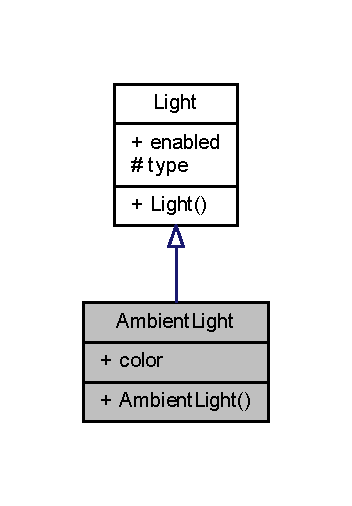
\includegraphics[width=169pt]{struct_ambient_light__inherit__graph}
\end{center}
\end{figure}


Collaboration diagram for Ambient\+Light\+:\nopagebreak
\begin{figure}[H]
\begin{center}
\leavevmode
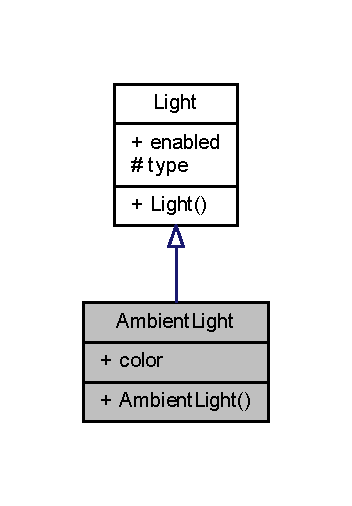
\includegraphics[width=169pt]{struct_ambient_light__coll__graph}
\end{center}
\end{figure}
\subsection*{Public Member Functions}
\begin{DoxyCompactItemize}
\item 
\hyperlink{struct_ambient_light_af6960d19d0e491643fef45009ba73437}{Ambient\+Light} (\hyperlink{_types_8h_a3d0ce73e3199de81565fb01632415288}{vec3} const \&light\+Color=\hyperlink{_types_8h_a3d0ce73e3199de81565fb01632415288}{vec3}(1.\+0f, 1.\+0f, 1.\+0f), bool light\+Enabled=true)
\end{DoxyCompactItemize}
\subsection*{Public Attributes}
\begin{DoxyCompactItemize}
\item 
\hyperlink{_types_8h_a3d0ce73e3199de81565fb01632415288}{vec3} \hyperlink{struct_ambient_light_af89096906b189fc10a3960b6e5f9b44c}{color}
\end{DoxyCompactItemize}
\subsection*{Additional Inherited Members}


\subsection{Detailed Description}


Definition at line 38 of file Light.\+h.



\subsection{Constructor \& Destructor Documentation}
\index{Ambient\+Light@{Ambient\+Light}!Ambient\+Light@{Ambient\+Light}}
\index{Ambient\+Light@{Ambient\+Light}!Ambient\+Light@{Ambient\+Light}}
\subsubsection[{\texorpdfstring{Ambient\+Light(vec3 const \&light\+Color=vec3(1.\+0f, 1.\+0f, 1.\+0f), bool light\+Enabled=true)}{AmbientLight(vec3 const &lightColor=vec3(1.0f, 1.0f, 1.0f), bool lightEnabled=true)}}]{\setlength{\rightskip}{0pt plus 5cm}Ambient\+Light\+::\+Ambient\+Light (
\begin{DoxyParamCaption}
\item[{{\bf vec3} const \&}]{light\+Color = {\ttfamily {\bf vec3}(1.0f,1.0f,1.0f)}, }
\item[{bool}]{light\+Enabled = {\ttfamily true}}
\end{DoxyParamCaption}
)\hspace{0.3cm}{\ttfamily [inline]}}\hypertarget{struct_ambient_light_af6960d19d0e491643fef45009ba73437}{}\label{struct_ambient_light_af6960d19d0e491643fef45009ba73437}


Definition at line 40 of file Light.\+h.



References Ambient\+Light(), Light\+::\+Light(), and L\+T\+\_\+\+Ambient.



Referenced by Ambient\+Light().


\begin{DoxyCode}
41     : \hyperlink{struct_light_a0df5e58af351bd13c996da2880be0dee}{Light}(\hyperlink{_light_8h_a3336214f41ddc8acd932fa9be957047da7f5cad38d8883da3c4cf77417530eebe}{LT\_Ambient}, lightEnabled)
42     , \hyperlink{struct_ambient_light_af89096906b189fc10a3960b6e5f9b44c}{color}(lightColor)
43   \{
44 
45   \}
\end{DoxyCode}


Here is the call graph for this function\+:\nopagebreak
\begin{figure}[H]
\begin{center}
\leavevmode
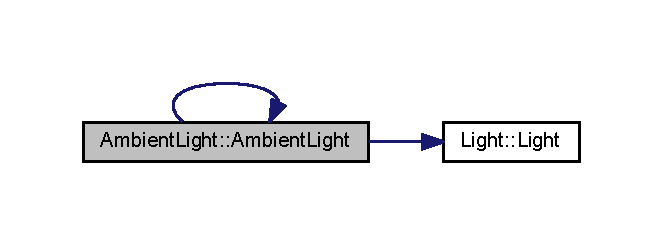
\includegraphics[width=318pt]{struct_ambient_light_af6960d19d0e491643fef45009ba73437_cgraph}
\end{center}
\end{figure}




Here is the caller graph for this function\+:\nopagebreak
\begin{figure}[H]
\begin{center}
\leavevmode
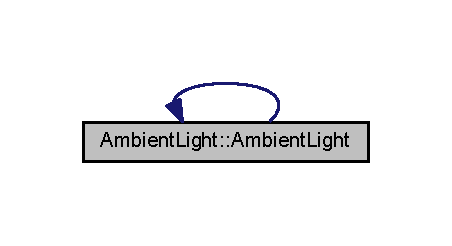
\includegraphics[width=217pt]{struct_ambient_light_af6960d19d0e491643fef45009ba73437_icgraph}
\end{center}
\end{figure}




\subsection{Member Data Documentation}
\index{Ambient\+Light@{Ambient\+Light}!color@{color}}
\index{color@{color}!Ambient\+Light@{Ambient\+Light}}
\subsubsection[{\texorpdfstring{color}{color}}]{\setlength{\rightskip}{0pt plus 5cm}{\bf vec3} Ambient\+Light\+::color}\hypertarget{struct_ambient_light_af89096906b189fc10a3960b6e5f9b44c}{}\label{struct_ambient_light_af89096906b189fc10a3960b6e5f9b44c}


Definition at line 46 of file Light.\+h.



The documentation for this struct was generated from the following file\+:\begin{DoxyCompactItemize}
\item 
C\+:/\+Users/elizabeth/\+Documents/\+Git\+Hub/\+Engine/\+Open\+G\+L\+Engine/\+Open\+G\+L\+Engine/\hyperlink{_light_8h}{Light.\+h}\end{DoxyCompactItemize}

\hypertarget{class_animation}{}\section{Animation Class Reference}
\label{class_animation}\index{Animation@{Animation}}


{\ttfamily \#include $<$Animation.\+h$>$}



Collaboration diagram for Animation\+:\nopagebreak
\begin{figure}[H]
\begin{center}
\leavevmode
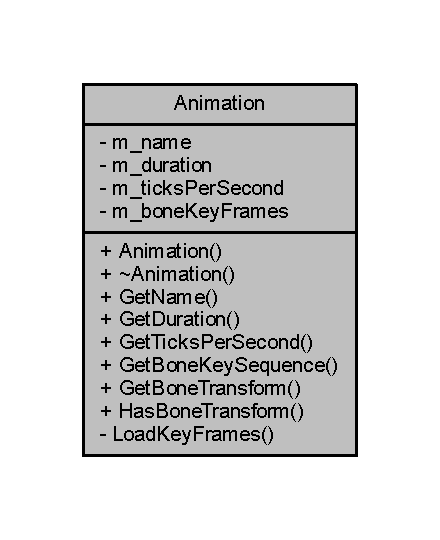
\includegraphics[width=211pt]{class_animation__coll__graph}
\end{center}
\end{figure}
\subsection*{Public Member Functions}
\begin{DoxyCompactItemize}
\item 
\hyperlink{class_animation_af4a62f49466ad950d2134ec8db003777}{Animation} (ai\+Animation const $\ast$p\+Animation, \hyperlink{class_bimap}{Bimap}$<$ \hyperlink{_types_8h_ad453f9f71ce1f9153fb748d6bb25e454}{string}, int $>$ const \&bone\+Lookup)
\begin{DoxyCompactList}\small\item\em Initializes a new instance of the \hyperlink{class_animation}{Animation} class. \end{DoxyCompactList}\item 
\hyperlink{class_animation_a401b68793d4fbf48d481c030ee4b2a16}{$\sim$\+Animation} ()
\item 
\hyperlink{_types_8h_ad453f9f71ce1f9153fb748d6bb25e454}{string} const \& \hyperlink{class_animation_abde46b2060b07d55958d1aad03291891}{Get\+Name} () const 
\begin{DoxyCompactList}\small\item\em Gets the name. \end{DoxyCompactList}\item 
float \hyperlink{class_animation_aa6f41b8a36928b2ea0a45f1ab711f988}{Get\+Duration} () const 
\begin{DoxyCompactList}\small\item\em Gets the duration. \end{DoxyCompactList}\item 
float \hyperlink{class_animation_a6db85fc750b517c596e06620080c864a}{Get\+Ticks\+Per\+Second} () const 
\begin{DoxyCompactList}\small\item\em Gets the ticks per second. \end{DoxyCompactList}\item 
\hyperlink{class_bone_key_sequence}{Bone\+Key\+Sequence} const \& \hyperlink{class_animation_a05bf490bf9e0903d027b28d393d31f4f}{Get\+Bone\+Key\+Sequence} (int bone\+ID) const 
\begin{DoxyCompactList}\small\item\em Gets the bone key sequence. \end{DoxyCompactList}\item 
\hyperlink{_types_8h_a2db59f395fe82a7394c6324956c265d8}{mat4} \hyperlink{class_animation_ae41ca205ccc04bfd62ea8df3531871b5}{Get\+Bone\+Transform} (int bone\+ID, float time) const 
\begin{DoxyCompactList}\small\item\em Gets the bone transform. \end{DoxyCompactList}\item 
bool \hyperlink{class_animation_a0c648eb3fe2e493dcd8748b9e3fd25de}{Has\+Bone\+Transform} (int bone\+ID) const 
\begin{DoxyCompactList}\small\item\em Determines whether \mbox{[}has bone transform\mbox{]} \mbox{[}the specified bone identifier\mbox{]}. \end{DoxyCompactList}\end{DoxyCompactItemize}
\subsection*{Private Member Functions}
\begin{DoxyCompactItemize}
\item 
void \hyperlink{class_animation_a49ed3e1b94f6b2e98052071a61aac4a5}{Load\+Key\+Frames} (ai\+Animation const $\ast$p\+Animation, \hyperlink{class_bimap}{Bimap}$<$ \hyperlink{_types_8h_ad453f9f71ce1f9153fb748d6bb25e454}{string}, int $>$ const \&bone\+Lookup)
\begin{DoxyCompactList}\small\item\em Loads the key frames. \end{DoxyCompactList}\end{DoxyCompactItemize}
\subsection*{Private Attributes}
\begin{DoxyCompactItemize}
\item 
\hyperlink{_types_8h_ad453f9f71ce1f9153fb748d6bb25e454}{string} \hyperlink{class_animation_adda9052e1e245ea1c5f1bcb02557ef32}{m\+\_\+name}
\begin{DoxyCompactList}\small\item\em The name \end{DoxyCompactList}\item 
float \hyperlink{class_animation_af74df305fff20e019837dd3f2351befa}{m\+\_\+duration}
\begin{DoxyCompactList}\small\item\em The duration \end{DoxyCompactList}\item 
float \hyperlink{class_animation_aed0aa67f96c0f3ca518e597ae683f791}{m\+\_\+ticks\+Per\+Second}
\begin{DoxyCompactList}\small\item\em The ticks per second \end{DoxyCompactList}\item 
std\+::unordered\+\_\+map$<$ int, std\+::unique\+\_\+ptr$<$ \hyperlink{class_bone_key_sequence}{Bone\+Key\+Sequence} $>$ $>$ \hyperlink{class_animation_a60b1ec3d3b1c19d6682b0e17d41be5e8}{m\+\_\+bone\+Key\+Frames}
\begin{DoxyCompactList}\small\item\em The bone key frames. \end{DoxyCompactList}\end{DoxyCompactItemize}


\subsection{Detailed Description}


Definition at line 25 of file Animation.\+h.



\subsection{Constructor \& Destructor Documentation}
\index{Animation@{Animation}!Animation@{Animation}}
\index{Animation@{Animation}!Animation@{Animation}}
\subsubsection[{\texorpdfstring{Animation(ai\+Animation const $\ast$p\+Animation, Bimap$<$ string, int $>$ const \&bone\+Lookup)}{Animation(aiAnimation const *pAnimation, Bimap< string, int > const &boneLookup)}}]{\setlength{\rightskip}{0pt plus 5cm}Animation\+::\+Animation (
\begin{DoxyParamCaption}
\item[{ai\+Animation const $\ast$}]{p\+Animation, }
\item[{{\bf Bimap}$<$ {\bf string}, int $>$ const \&}]{bone\+Lookup}
\end{DoxyParamCaption}
)}\hypertarget{class_animation_af4a62f49466ad950d2134ec8db003777}{}\label{class_animation_af4a62f49466ad950d2134ec8db003777}


Initializes a new instance of the \hyperlink{class_animation}{Animation} class. 


\begin{DoxyParams}{Parameters}
{\em p\+Animation} & The pointer to the animation.\\
\hline
{\em bone\+Lookup} & The bone lookup.\\
\hline
\end{DoxyParams}


Definition at line 5 of file Animation.\+cpp.



References Load\+Key\+Frames().


\begin{DoxyCode}
6 \{
7   \hyperlink{class_animation_adda9052e1e245ea1c5f1bcb02557ef32}{m\_name} = pAnimation->mName.data;
8   \hyperlink{class_animation_af74df305fff20e019837dd3f2351befa}{m\_duration} = float(pAnimation->mDuration);
9   \hyperlink{class_animation_aed0aa67f96c0f3ca518e597ae683f791}{m\_ticksPerSecond} = float(pAnimation->mTicksPerSecond);
10   \hyperlink{class_animation_a49ed3e1b94f6b2e98052071a61aac4a5}{LoadKeyFrames}(pAnimation, boneLookup);
11 \}
\end{DoxyCode}


Here is the call graph for this function\+:\nopagebreak
\begin{figure}[H]
\begin{center}
\leavevmode
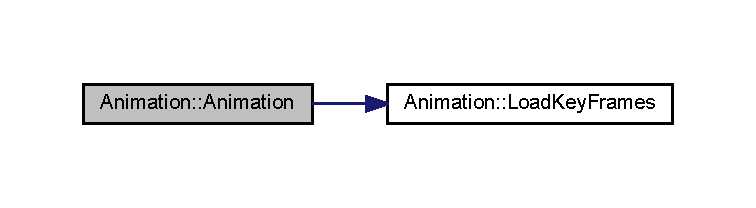
\includegraphics[width=350pt]{class_animation_af4a62f49466ad950d2134ec8db003777_cgraph}
\end{center}
\end{figure}


\index{Animation@{Animation}!````~Animation@{$\sim$\+Animation}}
\index{````~Animation@{$\sim$\+Animation}!Animation@{Animation}}
\subsubsection[{\texorpdfstring{$\sim$\+Animation()}{~Animation()}}]{\setlength{\rightskip}{0pt plus 5cm}Animation\+::$\sim$\+Animation (
\begin{DoxyParamCaption}
{}
\end{DoxyParamCaption}
)}\hypertarget{class_animation_a401b68793d4fbf48d481c030ee4b2a16}{}\label{class_animation_a401b68793d4fbf48d481c030ee4b2a16}


Definition at line 13 of file Animation.\+cpp.


\begin{DoxyCode}
14 \{
15 
16 \}
\end{DoxyCode}


\subsection{Member Function Documentation}
\index{Animation@{Animation}!Get\+Bone\+Key\+Sequence@{Get\+Bone\+Key\+Sequence}}
\index{Get\+Bone\+Key\+Sequence@{Get\+Bone\+Key\+Sequence}!Animation@{Animation}}
\subsubsection[{\texorpdfstring{Get\+Bone\+Key\+Sequence(int bone\+I\+D) const }{GetBoneKeySequence(int boneID) const }}]{\setlength{\rightskip}{0pt plus 5cm}{\bf Bone\+Key\+Sequence} const \& Animation\+::\+Get\+Bone\+Key\+Sequence (
\begin{DoxyParamCaption}
\item[{int}]{bone\+ID}
\end{DoxyParamCaption}
) const}\hypertarget{class_animation_a05bf490bf9e0903d027b28d393d31f4f}{}\label{class_animation_a05bf490bf9e0903d027b28d393d31f4f}


Gets the bone key sequence. 


\begin{DoxyParams}{Parameters}
{\em bone\+ID} & The bone identifier.\\
\hline
\end{DoxyParams}
\begin{DoxyReturn}{Returns}
A constant reference to the \hyperlink{class_bone_key_sequence}{Bone\+Key\+Sequence}
\end{DoxyReturn}


Definition at line 33 of file Animation.\+cpp.


\begin{DoxyCode}
34 \{
35   \textcolor{keywordflow}{return} *\hyperlink{class_animation_a60b1ec3d3b1c19d6682b0e17d41be5e8}{m\_boneKeyFrames}.at(boneID);
36 \}
\end{DoxyCode}
\index{Animation@{Animation}!Get\+Bone\+Transform@{Get\+Bone\+Transform}}
\index{Get\+Bone\+Transform@{Get\+Bone\+Transform}!Animation@{Animation}}
\subsubsection[{\texorpdfstring{Get\+Bone\+Transform(int bone\+I\+D, float time) const }{GetBoneTransform(int boneID, float time) const }}]{\setlength{\rightskip}{0pt plus 5cm}{\bf mat4} Animation\+::\+Get\+Bone\+Transform (
\begin{DoxyParamCaption}
\item[{int}]{bone\+ID, }
\item[{float}]{time}
\end{DoxyParamCaption}
) const}\hypertarget{class_animation_ae41ca205ccc04bfd62ea8df3531871b5}{}\label{class_animation_ae41ca205ccc04bfd62ea8df3531871b5}


Gets the bone transform. 


\begin{DoxyParams}{Parameters}
{\em bone\+ID} & The bone identifier.\\
\hline
{\em time} & The time.\\
\hline
\end{DoxyParams}
\begin{DoxyReturn}{Returns}
mat4
\end{DoxyReturn}


Definition at line 38 of file Animation.\+cpp.


\begin{DoxyCode}
39 \{
40   \textcolor{keywordflow}{return} \hyperlink{class_animation_a60b1ec3d3b1c19d6682b0e17d41be5e8}{m\_boneKeyFrames}.at(boneID)->GetTransform(fmod(time * 
      \hyperlink{class_animation_aed0aa67f96c0f3ca518e597ae683f791}{m\_ticksPerSecond}, \hyperlink{class_animation_af74df305fff20e019837dd3f2351befa}{m\_duration}));
41 \}
\end{DoxyCode}
\index{Animation@{Animation}!Get\+Duration@{Get\+Duration}}
\index{Get\+Duration@{Get\+Duration}!Animation@{Animation}}
\subsubsection[{\texorpdfstring{Get\+Duration() const }{GetDuration() const }}]{\setlength{\rightskip}{0pt plus 5cm}float Animation\+::\+Get\+Duration (
\begin{DoxyParamCaption}
{}
\end{DoxyParamCaption}
) const}\hypertarget{class_animation_aa6f41b8a36928b2ea0a45f1ab711f988}{}\label{class_animation_aa6f41b8a36928b2ea0a45f1ab711f988}


Gets the duration. 

\begin{DoxyReturn}{Returns}
float
\end{DoxyReturn}


Definition at line 23 of file Animation.\+cpp.



References m\+\_\+duration.


\begin{DoxyCode}
24 \{
25   \textcolor{keywordflow}{return} \hyperlink{class_animation_af74df305fff20e019837dd3f2351befa}{m\_duration};
26 \}
\end{DoxyCode}
\index{Animation@{Animation}!Get\+Name@{Get\+Name}}
\index{Get\+Name@{Get\+Name}!Animation@{Animation}}
\subsubsection[{\texorpdfstring{Get\+Name() const }{GetName() const }}]{\setlength{\rightskip}{0pt plus 5cm}{\bf string} const \& Animation\+::\+Get\+Name (
\begin{DoxyParamCaption}
{}
\end{DoxyParamCaption}
) const}\hypertarget{class_animation_abde46b2060b07d55958d1aad03291891}{}\label{class_animation_abde46b2060b07d55958d1aad03291891}


Gets the name. 

\begin{DoxyReturn}{Returns}
string
\end{DoxyReturn}


Definition at line 18 of file Animation.\+cpp.


\begin{DoxyCode}
19 \{
20   \textcolor{keywordflow}{return} \hyperlink{class_animation_adda9052e1e245ea1c5f1bcb02557ef32}{m\_name};
21 \}
\end{DoxyCode}
\index{Animation@{Animation}!Get\+Ticks\+Per\+Second@{Get\+Ticks\+Per\+Second}}
\index{Get\+Ticks\+Per\+Second@{Get\+Ticks\+Per\+Second}!Animation@{Animation}}
\subsubsection[{\texorpdfstring{Get\+Ticks\+Per\+Second() const }{GetTicksPerSecond() const }}]{\setlength{\rightskip}{0pt plus 5cm}float Animation\+::\+Get\+Ticks\+Per\+Second (
\begin{DoxyParamCaption}
{}
\end{DoxyParamCaption}
) const}\hypertarget{class_animation_a6db85fc750b517c596e06620080c864a}{}\label{class_animation_a6db85fc750b517c596e06620080c864a}


Gets the ticks per second. 

\begin{DoxyReturn}{Returns}
float
\end{DoxyReturn}


Definition at line 28 of file Animation.\+cpp.



References m\+\_\+ticks\+Per\+Second.


\begin{DoxyCode}
29 \{
30   \textcolor{keywordflow}{return} \hyperlink{class_animation_aed0aa67f96c0f3ca518e597ae683f791}{m\_ticksPerSecond};
31 \}
\end{DoxyCode}
\index{Animation@{Animation}!Has\+Bone\+Transform@{Has\+Bone\+Transform}}
\index{Has\+Bone\+Transform@{Has\+Bone\+Transform}!Animation@{Animation}}
\subsubsection[{\texorpdfstring{Has\+Bone\+Transform(int bone\+I\+D) const }{HasBoneTransform(int boneID) const }}]{\setlength{\rightskip}{0pt plus 5cm}bool Animation\+::\+Has\+Bone\+Transform (
\begin{DoxyParamCaption}
\item[{int}]{bone\+ID}
\end{DoxyParamCaption}
) const}\hypertarget{class_animation_a0c648eb3fe2e493dcd8748b9e3fd25de}{}\label{class_animation_a0c648eb3fe2e493dcd8748b9e3fd25de}


Determines whether \mbox{[}has bone transform\mbox{]} \mbox{[}the specified bone identifier\mbox{]}. 


\begin{DoxyParams}{Parameters}
{\em bone\+ID} & The bone identifier.\\
\hline
\end{DoxyParams}
\begin{DoxyReturn}{Returns}
{\ttfamily true} if \mbox{[}has bone transform\mbox{]} \mbox{[}the specified bone identifier\mbox{]}; otherwise, {\ttfamily false}. 
\end{DoxyReturn}


Definition at line 43 of file Animation.\+cpp.


\begin{DoxyCode}
44 \{
45     \textcolor{keywordflow}{return} \hyperlink{class_animation_a60b1ec3d3b1c19d6682b0e17d41be5e8}{m\_boneKeyFrames}.find(boneID) != \hyperlink{class_animation_a60b1ec3d3b1c19d6682b0e17d41be5e8}{m\_boneKeyFrames}.end();
46 \}
\end{DoxyCode}
\index{Animation@{Animation}!Load\+Key\+Frames@{Load\+Key\+Frames}}
\index{Load\+Key\+Frames@{Load\+Key\+Frames}!Animation@{Animation}}
\subsubsection[{\texorpdfstring{Load\+Key\+Frames(ai\+Animation const $\ast$p\+Animation, Bimap$<$ string, int $>$ const \&bone\+Lookup)}{LoadKeyFrames(aiAnimation const *pAnimation, Bimap< string, int > const &boneLookup)}}]{\setlength{\rightskip}{0pt plus 5cm}void Animation\+::\+Load\+Key\+Frames (
\begin{DoxyParamCaption}
\item[{ai\+Animation const $\ast$}]{p\+Animation, }
\item[{{\bf Bimap}$<$ {\bf string}, int $>$ const \&}]{bone\+Lookup}
\end{DoxyParamCaption}
)\hspace{0.3cm}{\ttfamily [private]}}\hypertarget{class_animation_a49ed3e1b94f6b2e98052071a61aac4a5}{}\label{class_animation_a49ed3e1b94f6b2e98052071a61aac4a5}


Loads the key frames. 


\begin{DoxyParams}{Parameters}
{\em p\+Animation} & The pointer to the animation.\\
\hline
{\em bone\+Lookup} & The bone lookup.\\
\hline
\end{DoxyParams}


Definition at line 48 of file Animation.\+cpp.



Referenced by Animation().


\begin{DoxyCode}
49 \{
50     \textcolor{keywordflow}{for} (\hyperlink{_types_8h_a4f5fce8c1ef282264f9214809524d836}{uint} i = 0; i < pAnimation->mNumChannels; i++)
51     \{
52         \textcolor{keywordtype}{int} boneIndex = boneLookup.\hyperlink{class_bimap_a38d190f4016ae28f415014ef4e6c08da}{GetValue}(pAnimation->mChannels[i]->mNodeName.data);
53         \hyperlink{class_animation_a60b1ec3d3b1c19d6682b0e17d41be5e8}{m\_boneKeyFrames}.emplace(boneIndex, \textcolor{keyword}{new} \hyperlink{class_bone_key_sequence}{BoneKeySequence}(pAnimation->
      mChannels[i], boneIndex));
54     \}
55 
56 \}
\end{DoxyCode}


Here is the caller graph for this function\+:\nopagebreak
\begin{figure}[H]
\begin{center}
\leavevmode
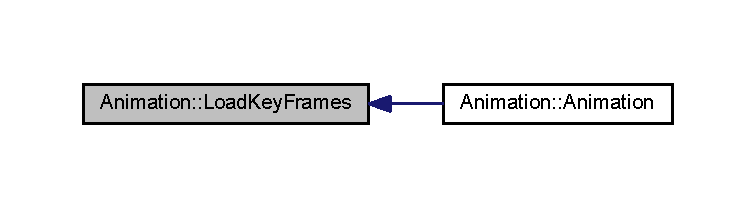
\includegraphics[width=350pt]{class_animation_a49ed3e1b94f6b2e98052071a61aac4a5_icgraph}
\end{center}
\end{figure}




\subsection{Member Data Documentation}
\index{Animation@{Animation}!m\+\_\+bone\+Key\+Frames@{m\+\_\+bone\+Key\+Frames}}
\index{m\+\_\+bone\+Key\+Frames@{m\+\_\+bone\+Key\+Frames}!Animation@{Animation}}
\subsubsection[{\texorpdfstring{m\+\_\+bone\+Key\+Frames}{m_boneKeyFrames}}]{\setlength{\rightskip}{0pt plus 5cm}std\+::unordered\+\_\+map$<$int, std\+::unique\+\_\+ptr$<${\bf Bone\+Key\+Sequence}$>$ $>$ Animation\+::m\+\_\+bone\+Key\+Frames\hspace{0.3cm}{\ttfamily [private]}}\hypertarget{class_animation_a60b1ec3d3b1c19d6682b0e17d41be5e8}{}\label{class_animation_a60b1ec3d3b1c19d6682b0e17d41be5e8}


The bone key frames. 



Definition at line 101 of file Animation.\+h.

\index{Animation@{Animation}!m\+\_\+duration@{m\+\_\+duration}}
\index{m\+\_\+duration@{m\+\_\+duration}!Animation@{Animation}}
\subsubsection[{\texorpdfstring{m\+\_\+duration}{m_duration}}]{\setlength{\rightskip}{0pt plus 5cm}float Animation\+::m\+\_\+duration\hspace{0.3cm}{\ttfamily [private]}}\hypertarget{class_animation_af74df305fff20e019837dd3f2351befa}{}\label{class_animation_af74df305fff20e019837dd3f2351befa}


The duration 



Definition at line 91 of file Animation.\+h.



Referenced by Get\+Duration().

\index{Animation@{Animation}!m\+\_\+name@{m\+\_\+name}}
\index{m\+\_\+name@{m\+\_\+name}!Animation@{Animation}}
\subsubsection[{\texorpdfstring{m\+\_\+name}{m_name}}]{\setlength{\rightskip}{0pt plus 5cm}{\bf string} Animation\+::m\+\_\+name\hspace{0.3cm}{\ttfamily [private]}}\hypertarget{class_animation_adda9052e1e245ea1c5f1bcb02557ef32}{}\label{class_animation_adda9052e1e245ea1c5f1bcb02557ef32}


The name 



Definition at line 86 of file Animation.\+h.

\index{Animation@{Animation}!m\+\_\+ticks\+Per\+Second@{m\+\_\+ticks\+Per\+Second}}
\index{m\+\_\+ticks\+Per\+Second@{m\+\_\+ticks\+Per\+Second}!Animation@{Animation}}
\subsubsection[{\texorpdfstring{m\+\_\+ticks\+Per\+Second}{m_ticksPerSecond}}]{\setlength{\rightskip}{0pt plus 5cm}float Animation\+::m\+\_\+ticks\+Per\+Second\hspace{0.3cm}{\ttfamily [private]}}\hypertarget{class_animation_aed0aa67f96c0f3ca518e597ae683f791}{}\label{class_animation_aed0aa67f96c0f3ca518e597ae683f791}


The ticks per second 



Definition at line 96 of file Animation.\+h.



Referenced by Get\+Ticks\+Per\+Second().



The documentation for this class was generated from the following files\+:\begin{DoxyCompactItemize}
\item 
C\+:/\+Users/elizabeth/\+Documents/\+Git\+Hub/\+Engine/\+Open\+G\+L\+Engine/\+Open\+G\+L\+Engine/\hyperlink{_animation_8h}{Animation.\+h}\item 
C\+:/\+Users/elizabeth/\+Documents/\+Git\+Hub/\+Engine/\+Open\+G\+L\+Engine/\+Open\+G\+L\+Engine/\hyperlink{_animation_8cpp}{Animation.\+cpp}\end{DoxyCompactItemize}

\hypertarget{class_bimap}{}\section{Bimap$<$ Key, Value $>$ Class Template Reference}
\label{class_bimap}\index{Bimap$<$ Key, Value $>$@{Bimap$<$ Key, Value $>$}}


{\ttfamily \#include $<$Bimap.\+h$>$}



Inheritance diagram for Bimap$<$ Key, Value $>$\+:\nopagebreak
\begin{figure}[H]
\begin{center}
\leavevmode
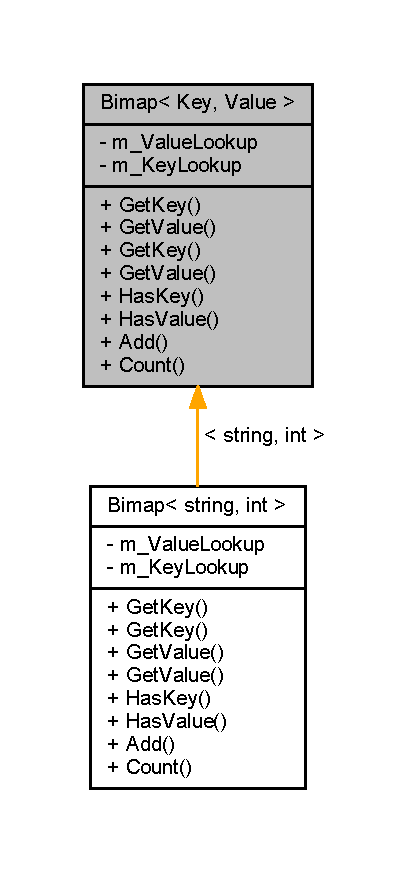
\includegraphics[width=197pt]{class_bimap__inherit__graph}
\end{center}
\end{figure}


Collaboration diagram for Bimap$<$ Key, Value $>$\+:\nopagebreak
\begin{figure}[H]
\begin{center}
\leavevmode
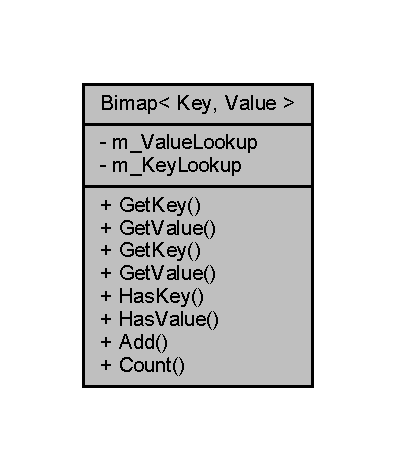
\includegraphics[width=190pt]{class_bimap__coll__graph}
\end{center}
\end{figure}
\subsection*{Public Member Functions}
\begin{DoxyCompactItemize}
\item 
Key \& \hyperlink{class_bimap_a287bee82ecf52e0addf01188e845b3b4}{Get\+Key} (const Value \&value)
\item 
Value \& \hyperlink{class_bimap_a38d190f4016ae28f415014ef4e6c08da}{Get\+Value} (const Key \&key)
\item 
Key const \& \hyperlink{class_bimap_a36a74e2ba009c5bc72dc3175db626395}{Get\+Key} (const Value \&value) const 
\item 
Value const \& \hyperlink{class_bimap_a094513ddbc939755ea3c26afa26c3975}{Get\+Value} (const Key \&key) const 
\item 
bool \hyperlink{class_bimap_acb0e0a0d4e926680f047edd90ee15f7b}{Has\+Key} (const Key \&key) const 
\item 
bool \hyperlink{class_bimap_a6aa7600cc5324041ba977670d85bbe4c}{Has\+Value} (const Value \&value) const 
\item 
void \hyperlink{class_bimap_a6c80d80555ca8318ee53845d83a81628}{Add} (const Key \&key, const Value \&value)
\item 
int \hyperlink{class_bimap_aef1a42d79e8c66d5453b655dc17ccc07}{Count} () const 
\end{DoxyCompactItemize}
\subsection*{Private Attributes}
\begin{DoxyCompactItemize}
\item 
std\+::unordered\+\_\+map$<$ Key, Value $>$ \hyperlink{class_bimap_ae27127063317d62ce8b44281e0804bb6}{m\+\_\+\+Value\+Lookup}
\item 
std\+::unordered\+\_\+map$<$ Value, Key $>$ \hyperlink{class_bimap_acc45f88d39f38379f4caf7a776b53f96}{m\+\_\+\+Key\+Lookup}
\end{DoxyCompactItemize}


\subsection{Detailed Description}
\subsubsection*{template$<$typename Key, typename Value$>$\\*
class Bimap$<$ Key, Value $>$}



Definition at line 7 of file Bimap.\+h.



\subsection{Member Function Documentation}
\index{Bimap@{Bimap}!Add@{Add}}
\index{Add@{Add}!Bimap@{Bimap}}
\subsubsection[{\texorpdfstring{Add(const Key \&key, const Value \&value)}{Add(const Key &key, const Value &value)}}]{\setlength{\rightskip}{0pt plus 5cm}template$<$typename Key, typename Value$>$ void {\bf Bimap}$<$ Key, Value $>$\+::Add (
\begin{DoxyParamCaption}
\item[{const Key \&}]{key, }
\item[{const Value \&}]{value}
\end{DoxyParamCaption}
)}\hypertarget{class_bimap_a6c80d80555ca8318ee53845d83a81628}{}\label{class_bimap_a6c80d80555ca8318ee53845d83a81628}


Definition at line 30 of file Bimap.\+h.


\begin{DoxyCode}
31 \{
32     \hyperlink{class_bimap_ae27127063317d62ce8b44281e0804bb6}{m\_ValueLookup}.emplace(key, value);
33     \hyperlink{class_bimap_acc45f88d39f38379f4caf7a776b53f96}{m\_KeyLookup}.emplace(value, key);
34 \}
\end{DoxyCode}
\index{Bimap@{Bimap}!Count@{Count}}
\index{Count@{Count}!Bimap@{Bimap}}
\subsubsection[{\texorpdfstring{Count() const }{Count() const }}]{\setlength{\rightskip}{0pt plus 5cm}template$<$typename Key , typename Value $>$ int {\bf Bimap}$<$ Key, Value $>$\+::Count (
\begin{DoxyParamCaption}
{}
\end{DoxyParamCaption}
) const}\hypertarget{class_bimap_aef1a42d79e8c66d5453b655dc17ccc07}{}\label{class_bimap_aef1a42d79e8c66d5453b655dc17ccc07}


Definition at line 73 of file Bimap.\+h.


\begin{DoxyCode}
74 \{
75     \textcolor{keywordflow}{return} \hyperlink{class_bimap_ae27127063317d62ce8b44281e0804bb6}{m\_ValueLookup}.size();
76 \}
\end{DoxyCode}
\index{Bimap@{Bimap}!Get\+Key@{Get\+Key}}
\index{Get\+Key@{Get\+Key}!Bimap@{Bimap}}
\subsubsection[{\texorpdfstring{Get\+Key(const Value \&value)}{GetKey(const Value &value)}}]{\setlength{\rightskip}{0pt plus 5cm}template$<$typename Key , typename Value$>$ Key \& {\bf Bimap}$<$ Key, Value $>$\+::Get\+Key (
\begin{DoxyParamCaption}
\item[{const Value \&}]{value}
\end{DoxyParamCaption}
)}\hypertarget{class_bimap_a287bee82ecf52e0addf01188e845b3b4}{}\label{class_bimap_a287bee82ecf52e0addf01188e845b3b4}


Definition at line 67 of file Bimap.\+h.


\begin{DoxyCode}
68 \{
69     \textcolor{keywordflow}{return} \hyperlink{class_bimap_acc45f88d39f38379f4caf7a776b53f96}{m\_KeyLookup}[value];
70 \}
\end{DoxyCode}
\index{Bimap@{Bimap}!Get\+Key@{Get\+Key}}
\index{Get\+Key@{Get\+Key}!Bimap@{Bimap}}
\subsubsection[{\texorpdfstring{Get\+Key(const Value \&value) const }{GetKey(const Value &value) const }}]{\setlength{\rightskip}{0pt plus 5cm}template$<$typename Key , typename Value$>$ Key const \& {\bf Bimap}$<$ Key, Value $>$\+::Get\+Key (
\begin{DoxyParamCaption}
\item[{const Value \&}]{value}
\end{DoxyParamCaption}
) const}\hypertarget{class_bimap_a36a74e2ba009c5bc72dc3175db626395}{}\label{class_bimap_a36a74e2ba009c5bc72dc3175db626395}


Definition at line 55 of file Bimap.\+h.


\begin{DoxyCode}
56 \{
57     \textcolor{keywordflow}{return} \hyperlink{class_bimap_acc45f88d39f38379f4caf7a776b53f96}{m\_KeyLookup}.at(value);
58 \}
\end{DoxyCode}
\index{Bimap@{Bimap}!Get\+Value@{Get\+Value}}
\index{Get\+Value@{Get\+Value}!Bimap@{Bimap}}
\subsubsection[{\texorpdfstring{Get\+Value(const Key \&key)}{GetValue(const Key &key)}}]{\setlength{\rightskip}{0pt plus 5cm}template$<$typename Key, typename Value $>$ Value \& {\bf Bimap}$<$ Key, Value $>$\+::Get\+Value (
\begin{DoxyParamCaption}
\item[{const Key \&}]{key}
\end{DoxyParamCaption}
)}\hypertarget{class_bimap_a38d190f4016ae28f415014ef4e6c08da}{}\label{class_bimap_a38d190f4016ae28f415014ef4e6c08da}


Definition at line 61 of file Bimap.\+h.


\begin{DoxyCode}
62 \{
63     \textcolor{keywordflow}{return} \hyperlink{class_bimap_ae27127063317d62ce8b44281e0804bb6}{m\_ValueLookup}[key];
64 \}
\end{DoxyCode}
\index{Bimap@{Bimap}!Get\+Value@{Get\+Value}}
\index{Get\+Value@{Get\+Value}!Bimap@{Bimap}}
\subsubsection[{\texorpdfstring{Get\+Value(const Key \&key) const }{GetValue(const Key &key) const }}]{\setlength{\rightskip}{0pt plus 5cm}template$<$typename Key, typename Value $>$ Value const \& {\bf Bimap}$<$ Key, Value $>$\+::Get\+Value (
\begin{DoxyParamCaption}
\item[{const Key \&}]{key}
\end{DoxyParamCaption}
) const}\hypertarget{class_bimap_a094513ddbc939755ea3c26afa26c3975}{}\label{class_bimap_a094513ddbc939755ea3c26afa26c3975}


Definition at line 49 of file Bimap.\+h.


\begin{DoxyCode}
50 \{
51     \textcolor{keywordflow}{return} \hyperlink{class_bimap_ae27127063317d62ce8b44281e0804bb6}{m\_ValueLookup}.at(key);
52 \}
\end{DoxyCode}
\index{Bimap@{Bimap}!Has\+Key@{Has\+Key}}
\index{Has\+Key@{Has\+Key}!Bimap@{Bimap}}
\subsubsection[{\texorpdfstring{Has\+Key(const Key \&key) const }{HasKey(const Key &key) const }}]{\setlength{\rightskip}{0pt plus 5cm}template$<$typename Key, typename Value $>$ bool {\bf Bimap}$<$ Key, Value $>$\+::Has\+Key (
\begin{DoxyParamCaption}
\item[{const Key \&}]{key}
\end{DoxyParamCaption}
) const}\hypertarget{class_bimap_acb0e0a0d4e926680f047edd90ee15f7b}{}\label{class_bimap_acb0e0a0d4e926680f047edd90ee15f7b}


Definition at line 43 of file Bimap.\+h.


\begin{DoxyCode}
44 \{
45     \textcolor{keywordflow}{return} \hyperlink{class_bimap_ae27127063317d62ce8b44281e0804bb6}{m\_ValueLookup}.find(key) != \hyperlink{class_bimap_ae27127063317d62ce8b44281e0804bb6}{m\_ValueLookup}.end();
46 \}
\end{DoxyCode}
\index{Bimap@{Bimap}!Has\+Value@{Has\+Value}}
\index{Has\+Value@{Has\+Value}!Bimap@{Bimap}}
\subsubsection[{\texorpdfstring{Has\+Value(const Value \&value) const }{HasValue(const Value &value) const }}]{\setlength{\rightskip}{0pt plus 5cm}template$<$typename Key , typename Value$>$ bool {\bf Bimap}$<$ Key, Value $>$\+::Has\+Value (
\begin{DoxyParamCaption}
\item[{const Value \&}]{value}
\end{DoxyParamCaption}
) const}\hypertarget{class_bimap_a6aa7600cc5324041ba977670d85bbe4c}{}\label{class_bimap_a6aa7600cc5324041ba977670d85bbe4c}


Definition at line 37 of file Bimap.\+h.


\begin{DoxyCode}
38 \{
39     \textcolor{keywordflow}{return} \hyperlink{class_bimap_acc45f88d39f38379f4caf7a776b53f96}{m\_KeyLookup}.find(value) != \hyperlink{class_bimap_acc45f88d39f38379f4caf7a776b53f96}{m\_KeyLookup}.end();
40 \}
\end{DoxyCode}


\subsection{Member Data Documentation}
\index{Bimap@{Bimap}!m\+\_\+\+Key\+Lookup@{m\+\_\+\+Key\+Lookup}}
\index{m\+\_\+\+Key\+Lookup@{m\+\_\+\+Key\+Lookup}!Bimap@{Bimap}}
\subsubsection[{\texorpdfstring{m\+\_\+\+Key\+Lookup}{m_KeyLookup}}]{\setlength{\rightskip}{0pt plus 5cm}template$<$typename Key, typename Value$>$ std\+::unordered\+\_\+map$<$Value, Key$>$ {\bf Bimap}$<$ Key, Value $>$\+::m\+\_\+\+Key\+Lookup\hspace{0.3cm}{\ttfamily [private]}}\hypertarget{class_bimap_acc45f88d39f38379f4caf7a776b53f96}{}\label{class_bimap_acc45f88d39f38379f4caf7a776b53f96}


Definition at line 26 of file Bimap.\+h.

\index{Bimap@{Bimap}!m\+\_\+\+Value\+Lookup@{m\+\_\+\+Value\+Lookup}}
\index{m\+\_\+\+Value\+Lookup@{m\+\_\+\+Value\+Lookup}!Bimap@{Bimap}}
\subsubsection[{\texorpdfstring{m\+\_\+\+Value\+Lookup}{m_ValueLookup}}]{\setlength{\rightskip}{0pt plus 5cm}template$<$typename Key, typename Value$>$ std\+::unordered\+\_\+map$<$Key, Value$>$ {\bf Bimap}$<$ Key, Value $>$\+::m\+\_\+\+Value\+Lookup\hspace{0.3cm}{\ttfamily [private]}}\hypertarget{class_bimap_ae27127063317d62ce8b44281e0804bb6}{}\label{class_bimap_ae27127063317d62ce8b44281e0804bb6}


Definition at line 25 of file Bimap.\+h.



The documentation for this class was generated from the following file\+:\begin{DoxyCompactItemize}
\item 
C\+:/\+Users/elizabeth/\+Documents/\+Git\+Hub/\+Engine/\+Open\+G\+L\+Engine/\+Open\+G\+L\+Engine/\hyperlink{_bimap_8h}{Bimap.\+h}\end{DoxyCompactItemize}

\hypertarget{class_bloom_effect}{}\section{Bloom\+Effect Class Reference}
\label{class_bloom_effect}\index{Bloom\+Effect@{Bloom\+Effect}}


{\ttfamily \#include $<$Bloom\+Effect.\+h$>$}



Collaboration diagram for Bloom\+Effect\+:\nopagebreak
\begin{figure}[H]
\begin{center}
\leavevmode
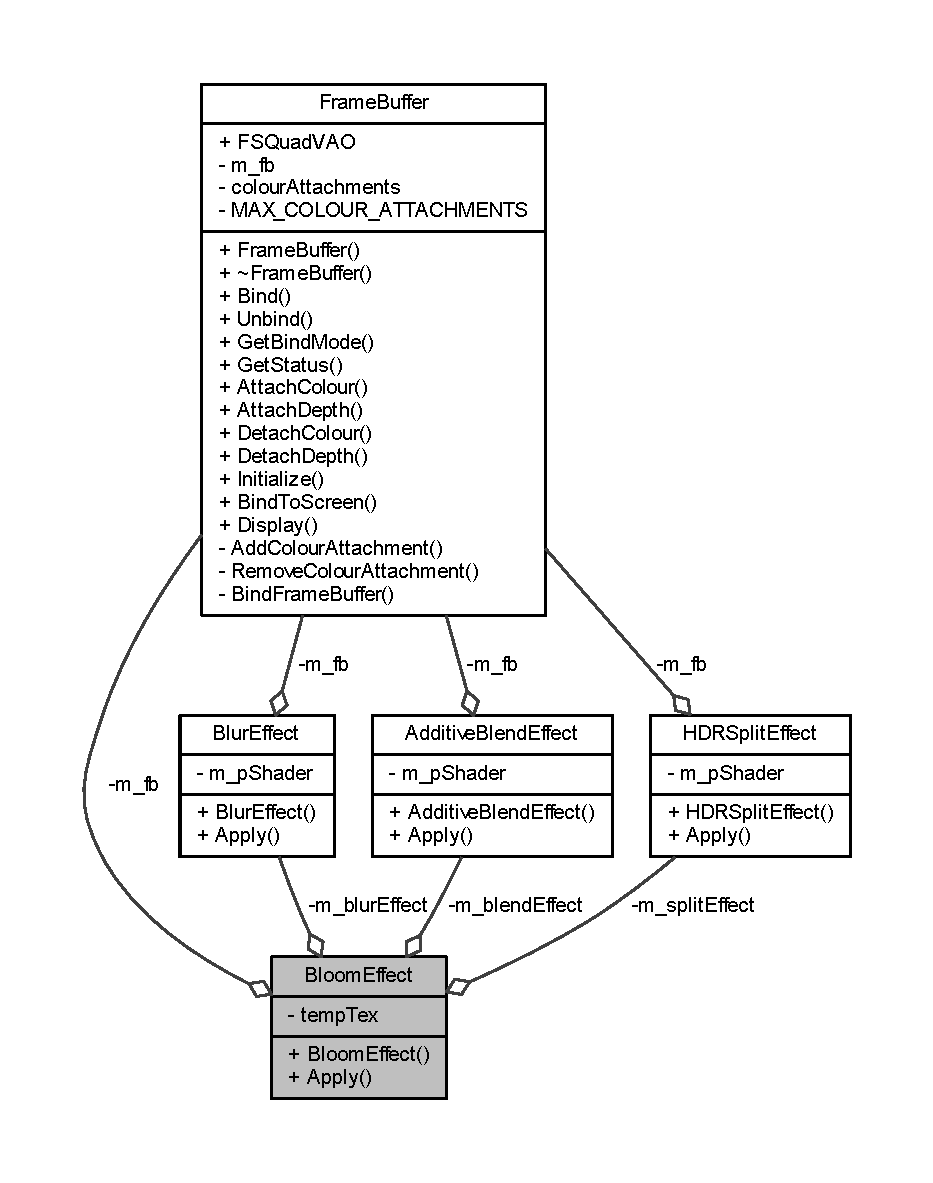
\includegraphics[width=350pt]{class_bloom_effect__coll__graph}
\end{center}
\end{figure}
\subsection*{Public Member Functions}
\begin{DoxyCompactItemize}
\item 
\hyperlink{class_bloom_effect_ae76d6ede7ad9201f6bf8f4c9927c827b}{Bloom\+Effect} ()
\item 
void \hyperlink{class_bloom_effect_ace516d6debe768f05d147089f6927026}{Apply} (G\+Luint input\+Tex, G\+Luint ouput\+Tex, int bloom\+Radius)
\begin{DoxyCompactList}\small\item\em Applies the bloom effect. \end{DoxyCompactList}\end{DoxyCompactItemize}
\subsection*{Private Attributes}
\begin{DoxyCompactItemize}
\item 
\hyperlink{class_frame_buffer}{Frame\+Buffer} \hyperlink{class_bloom_effect_a6e92b45d7d260f5aa0dcf3a299b28cfe}{m\+\_\+fb}
\begin{DoxyCompactList}\small\item\em The frame buffer \end{DoxyCompactList}\item 
\hyperlink{class_h_d_r_split_effect}{H\+D\+R\+Split\+Effect} \hyperlink{class_bloom_effect_aabecb4a9b579674d07806b3676a26d52}{m\+\_\+split\+Effect}
\begin{DoxyCompactList}\small\item\em The split effect \end{DoxyCompactList}\item 
\hyperlink{class_blur_effect}{Blur\+Effect} \hyperlink{class_bloom_effect_abc532338b21e4a70dac9a4e98bff00ae}{m\+\_\+blur\+Effect}
\begin{DoxyCompactList}\small\item\em The blur effect \end{DoxyCompactList}\item 
\hyperlink{class_additive_blend_effect}{Additive\+Blend\+Effect} \hyperlink{class_bloom_effect_a2227e1cb8bf17f584ef22b8320d4bf01}{m\+\_\+blend\+Effect}
\begin{DoxyCompactList}\small\item\em The blend effect \end{DoxyCompactList}\item 
G\+Luint \hyperlink{class_bloom_effect_a74ea9780de0ea8954b981dbaa61b3aa4}{temp\+Tex} \mbox{[}3\mbox{]}
\begin{DoxyCompactList}\small\item\em The temporary textures \end{DoxyCompactList}\end{DoxyCompactItemize}


\subsection{Detailed Description}


Definition at line 20 of file Bloom\+Effect.\+h.



\subsection{Constructor \& Destructor Documentation}
\index{Bloom\+Effect@{Bloom\+Effect}!Bloom\+Effect@{Bloom\+Effect}}
\index{Bloom\+Effect@{Bloom\+Effect}!Bloom\+Effect@{Bloom\+Effect}}
\subsubsection[{\texorpdfstring{Bloom\+Effect()}{BloomEffect()}}]{\setlength{\rightskip}{0pt plus 5cm}Bloom\+Effect\+::\+Bloom\+Effect (
\begin{DoxyParamCaption}
{}
\end{DoxyParamCaption}
)}\hypertarget{class_bloom_effect_ae76d6ede7ad9201f6bf8f4c9927c827b}{}\label{class_bloom_effect_ae76d6ede7ad9201f6bf8f4c9927c827b}


Definition at line 4 of file Bloom\+Effect.\+cpp.



Referenced by Render\+Manager\+A\+P\+I\+::\+Initialise().


\begin{DoxyCode}
5 \{
6   \textcolor{keywordflow}{for} (\textcolor{keywordtype}{int} i = 0; i < 3; i++)
7     \hyperlink{class_bloom_effect_a74ea9780de0ea8954b981dbaa61b3aa4}{tempTex}[i] = \hyperlink{_texture_8h_a50d476cb6e78d47146e686e2f6da2a1e}{CreateVec3Texture}();
8 \}
\end{DoxyCode}


Here is the caller graph for this function\+:
\nopagebreak
\begin{figure}[H]
\begin{center}
\leavevmode
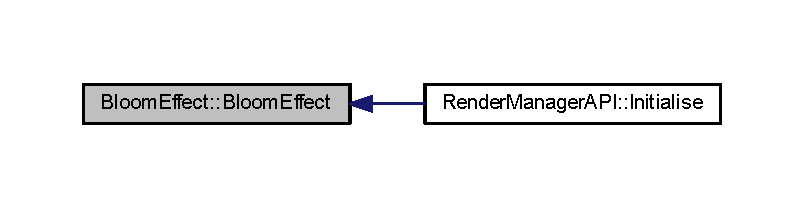
\includegraphics[width=350pt]{class_bloom_effect_ae76d6ede7ad9201f6bf8f4c9927c827b_icgraph}
\end{center}
\end{figure}




\subsection{Member Function Documentation}
\index{Bloom\+Effect@{Bloom\+Effect}!Apply@{Apply}}
\index{Apply@{Apply}!Bloom\+Effect@{Bloom\+Effect}}
\subsubsection[{\texorpdfstring{Apply(\+G\+Luint input\+Tex, G\+Luint ouput\+Tex, int bloom\+Radius)}{Apply(GLuint inputTex, GLuint ouputTex, int bloomRadius)}}]{\setlength{\rightskip}{0pt plus 5cm}void Bloom\+Effect\+::\+Apply (
\begin{DoxyParamCaption}
\item[{G\+Luint}]{input\+Tex, }
\item[{G\+Luint}]{ouput\+Tex, }
\item[{int}]{bloom\+Radius}
\end{DoxyParamCaption}
)}\hypertarget{class_bloom_effect_ace516d6debe768f05d147089f6927026}{}\label{class_bloom_effect_ace516d6debe768f05d147089f6927026}


Applies the bloom effect. 


\begin{DoxyParams}{Parameters}
{\em input\+Tex} & The input tex.\\
\hline
{\em ouput\+Tex} & The ouput tex.\\
\hline
{\em bloom\+Radius} & The bloom radius.\\
\hline
\end{DoxyParams}


Definition at line 10 of file Bloom\+Effect.\+cpp.


\begin{DoxyCode}
11 \{
12   \hyperlink{class_bloom_effect_aabecb4a9b579674d07806b3676a26d52}{m\_splitEffect}.\hyperlink{class_h_d_r_split_effect_ab2f8295e2f9efbfe5889c837c4c1854e}{Apply}(inputTex, \hyperlink{class_bloom_effect_a74ea9780de0ea8954b981dbaa61b3aa4}{tempTex}[0], \hyperlink{class_bloom_effect_a74ea9780de0ea8954b981dbaa61b3aa4}{tempTex}[1]);
13   \hyperlink{class_bloom_effect_abc532338b21e4a70dac9a4e98bff00ae}{m\_blurEffect}.\hyperlink{class_blur_effect_af9aced52cdc0360bf8a424cf49802d92}{Apply}(\hyperlink{class_bloom_effect_a74ea9780de0ea8954b981dbaa61b3aa4}{tempTex}[1], \hyperlink{class_bloom_effect_a74ea9780de0ea8954b981dbaa61b3aa4}{tempTex}[2], bloomRadius);
14   \hyperlink{class_bloom_effect_abc532338b21e4a70dac9a4e98bff00ae}{m\_blurEffect}.\hyperlink{class_blur_effect_af9aced52cdc0360bf8a424cf49802d92}{Apply}(\hyperlink{class_bloom_effect_a74ea9780de0ea8954b981dbaa61b3aa4}{tempTex}[2], \hyperlink{class_bloom_effect_a74ea9780de0ea8954b981dbaa61b3aa4}{tempTex}[1], bloomRadius);
15   \hyperlink{class_bloom_effect_abc532338b21e4a70dac9a4e98bff00ae}{m\_blurEffect}.\hyperlink{class_blur_effect_af9aced52cdc0360bf8a424cf49802d92}{Apply}(\hyperlink{class_bloom_effect_a74ea9780de0ea8954b981dbaa61b3aa4}{tempTex}[1], \hyperlink{class_bloom_effect_a74ea9780de0ea8954b981dbaa61b3aa4}{tempTex}[2], bloomRadius);
16   \hyperlink{class_bloom_effect_a2227e1cb8bf17f584ef22b8320d4bf01}{m\_blendEffect}.\hyperlink{class_additive_blend_effect_a9e75b87d6e8bf28acc4f5d31c3049453}{Apply}(\hyperlink{class_bloom_effect_a74ea9780de0ea8954b981dbaa61b3aa4}{tempTex}[0], \hyperlink{class_bloom_effect_a74ea9780de0ea8954b981dbaa61b3aa4}{tempTex}[2], outputTex);
17 \}
\end{DoxyCode}


\subsection{Member Data Documentation}
\index{Bloom\+Effect@{Bloom\+Effect}!m\+\_\+blend\+Effect@{m\+\_\+blend\+Effect}}
\index{m\+\_\+blend\+Effect@{m\+\_\+blend\+Effect}!Bloom\+Effect@{Bloom\+Effect}}
\subsubsection[{\texorpdfstring{m\+\_\+blend\+Effect}{m_blendEffect}}]{\setlength{\rightskip}{0pt plus 5cm}{\bf Additive\+Blend\+Effect} Bloom\+Effect\+::m\+\_\+blend\+Effect\hspace{0.3cm}{\ttfamily [private]}}\hypertarget{class_bloom_effect_a2227e1cb8bf17f584ef22b8320d4bf01}{}\label{class_bloom_effect_a2227e1cb8bf17f584ef22b8320d4bf01}


The blend effect 



Definition at line 55 of file Bloom\+Effect.\+h.

\index{Bloom\+Effect@{Bloom\+Effect}!m\+\_\+blur\+Effect@{m\+\_\+blur\+Effect}}
\index{m\+\_\+blur\+Effect@{m\+\_\+blur\+Effect}!Bloom\+Effect@{Bloom\+Effect}}
\subsubsection[{\texorpdfstring{m\+\_\+blur\+Effect}{m_blurEffect}}]{\setlength{\rightskip}{0pt plus 5cm}{\bf Blur\+Effect} Bloom\+Effect\+::m\+\_\+blur\+Effect\hspace{0.3cm}{\ttfamily [private]}}\hypertarget{class_bloom_effect_abc532338b21e4a70dac9a4e98bff00ae}{}\label{class_bloom_effect_abc532338b21e4a70dac9a4e98bff00ae}


The blur effect 



Definition at line 50 of file Bloom\+Effect.\+h.

\index{Bloom\+Effect@{Bloom\+Effect}!m\+\_\+fb@{m\+\_\+fb}}
\index{m\+\_\+fb@{m\+\_\+fb}!Bloom\+Effect@{Bloom\+Effect}}
\subsubsection[{\texorpdfstring{m\+\_\+fb}{m_fb}}]{\setlength{\rightskip}{0pt plus 5cm}{\bf Frame\+Buffer} Bloom\+Effect\+::m\+\_\+fb\hspace{0.3cm}{\ttfamily [private]}}\hypertarget{class_bloom_effect_a6e92b45d7d260f5aa0dcf3a299b28cfe}{}\label{class_bloom_effect_a6e92b45d7d260f5aa0dcf3a299b28cfe}


The frame buffer 



Definition at line 40 of file Bloom\+Effect.\+h.

\index{Bloom\+Effect@{Bloom\+Effect}!m\+\_\+split\+Effect@{m\+\_\+split\+Effect}}
\index{m\+\_\+split\+Effect@{m\+\_\+split\+Effect}!Bloom\+Effect@{Bloom\+Effect}}
\subsubsection[{\texorpdfstring{m\+\_\+split\+Effect}{m_splitEffect}}]{\setlength{\rightskip}{0pt plus 5cm}{\bf H\+D\+R\+Split\+Effect} Bloom\+Effect\+::m\+\_\+split\+Effect\hspace{0.3cm}{\ttfamily [private]}}\hypertarget{class_bloom_effect_aabecb4a9b579674d07806b3676a26d52}{}\label{class_bloom_effect_aabecb4a9b579674d07806b3676a26d52}


The split effect 



Definition at line 45 of file Bloom\+Effect.\+h.

\index{Bloom\+Effect@{Bloom\+Effect}!temp\+Tex@{temp\+Tex}}
\index{temp\+Tex@{temp\+Tex}!Bloom\+Effect@{Bloom\+Effect}}
\subsubsection[{\texorpdfstring{temp\+Tex}{tempTex}}]{\setlength{\rightskip}{0pt plus 5cm}G\+Luint Bloom\+Effect\+::temp\+Tex\mbox{[}3\mbox{]}\hspace{0.3cm}{\ttfamily [private]}}\hypertarget{class_bloom_effect_a74ea9780de0ea8954b981dbaa61b3aa4}{}\label{class_bloom_effect_a74ea9780de0ea8954b981dbaa61b3aa4}


The temporary textures 



Definition at line 60 of file Bloom\+Effect.\+h.



Referenced by Render\+Manager\+A\+P\+I\+::\+Initialise().



The documentation for this class was generated from the following files\+:\begin{DoxyCompactItemize}
\item 
C\+:/\+Users/elizabeth/\+Documents/\+Git\+Hub/\+Engine/\+Open\+G\+L\+Engine/\+Open\+G\+L\+Engine/\hyperlink{_bloom_effect_8h}{Bloom\+Effect.\+h}\item 
C\+:/\+Users/elizabeth/\+Documents/\+Git\+Hub/\+Engine/\+Open\+G\+L\+Engine/\+Open\+G\+L\+Engine/\hyperlink{_bloom_effect_8cpp}{Bloom\+Effect.\+cpp}\end{DoxyCompactItemize}

\hypertarget{class_blur_effect}{}\section{Blur\+Effect Class Reference}
\label{class_blur_effect}\index{Blur\+Effect@{Blur\+Effect}}


{\ttfamily \#include $<$Blur\+Effect.\+h$>$}



Collaboration diagram for Blur\+Effect\+:\nopagebreak
\begin{figure}[H]
\begin{center}
\leavevmode
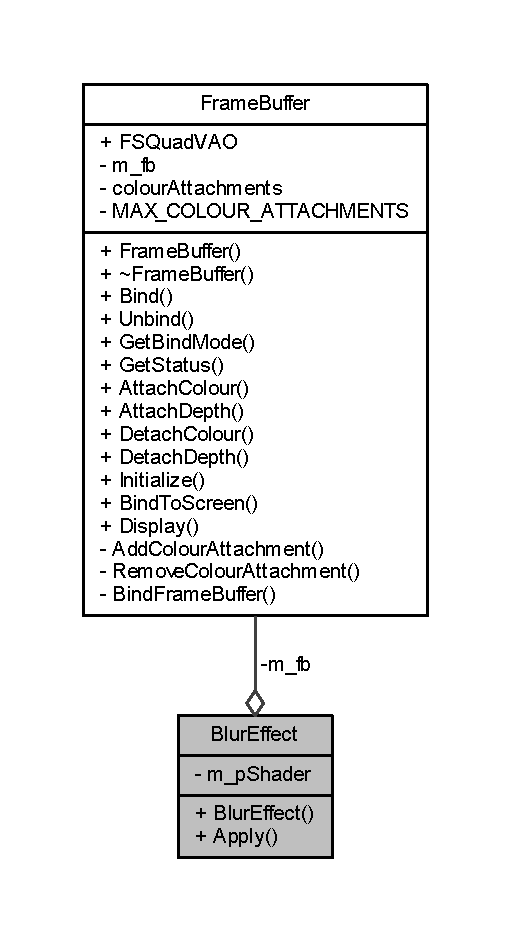
\includegraphics[width=245pt]{class_blur_effect__coll__graph}
\end{center}
\end{figure}
\subsection*{Public Member Functions}
\begin{DoxyCompactItemize}
\item 
\hyperlink{class_blur_effect_aad277452b90533f33dbd42bd55b8ed78}{Blur\+Effect} ()
\begin{DoxyCompactList}\small\item\em Initializes a new instance of the \hyperlink{class_blur_effect}{Blur\+Effect} class. \end{DoxyCompactList}\item 
void \hyperlink{class_blur_effect_af9aced52cdc0360bf8a424cf49802d92}{Apply} (G\+Luint input\+Tex, G\+Luint output\+Tex, int blur\+Radius)
\begin{DoxyCompactList}\small\item\em Applies the blur effect. \end{DoxyCompactList}\end{DoxyCompactItemize}
\subsection*{Private Attributes}
\begin{DoxyCompactItemize}
\item 
\hyperlink{class_frame_buffer}{Frame\+Buffer} \hyperlink{class_blur_effect_a73b9441bb187c47b83d99e2a67a421e5}{m\+\_\+fb}
\begin{DoxyCompactList}\small\item\em The frame buffer \end{DoxyCompactList}\item 
std\+::unique\+\_\+ptr$<$ \hyperlink{class_i_shader}{I\+Shader} $>$ const \& \hyperlink{class_blur_effect_a29dbaae4fbb90818efcabf0d02dbba01}{m\+\_\+p\+Shader}
\begin{DoxyCompactList}\small\item\em The shader \end{DoxyCompactList}\end{DoxyCompactItemize}


\subsection{Detailed Description}


Definition at line 17 of file Blur\+Effect.\+h.



\subsection{Constructor \& Destructor Documentation}
\index{Blur\+Effect@{Blur\+Effect}!Blur\+Effect@{Blur\+Effect}}
\index{Blur\+Effect@{Blur\+Effect}!Blur\+Effect@{Blur\+Effect}}
\subsubsection[{\texorpdfstring{Blur\+Effect()}{BlurEffect()}}]{\setlength{\rightskip}{0pt plus 5cm}Blur\+Effect\+::\+Blur\+Effect (
\begin{DoxyParamCaption}
{}
\end{DoxyParamCaption}
)}\hypertarget{class_blur_effect_aad277452b90533f33dbd42bd55b8ed78}{}\label{class_blur_effect_aad277452b90533f33dbd42bd55b8ed78}


Initializes a new instance of the \hyperlink{class_blur_effect}{Blur\+Effect} class. 



Definition at line 5 of file Blur\+Effect.\+cpp.



References Blur\+Effect().



Referenced by Blur\+Effect().


\begin{DoxyCode}
6   : \hyperlink{class_blur_effect_a29dbaae4fbb90818efcabf0d02dbba01}{m\_pShader}(\hyperlink{class_singleton_a74f32751d99bf3cc95fe17aba11f4b07}{ShaderLibrary::GetInstance}().GetShader(\textcolor{stringliteral}{"BlurEffect"}))
7 \{
8   
9 \}
\end{DoxyCode}


Here is the call graph for this function\+:\nopagebreak
\begin{figure}[H]
\begin{center}
\leavevmode
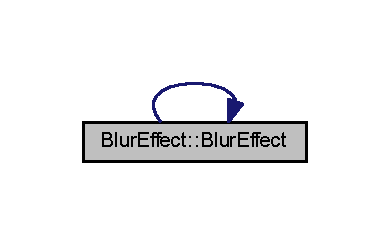
\includegraphics[width=187pt]{class_blur_effect_aad277452b90533f33dbd42bd55b8ed78_cgraph}
\end{center}
\end{figure}




Here is the caller graph for this function\+:\nopagebreak
\begin{figure}[H]
\begin{center}
\leavevmode
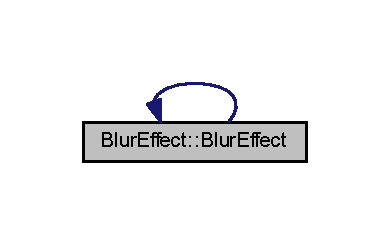
\includegraphics[width=187pt]{class_blur_effect_aad277452b90533f33dbd42bd55b8ed78_icgraph}
\end{center}
\end{figure}




\subsection{Member Function Documentation}
\index{Blur\+Effect@{Blur\+Effect}!Apply@{Apply}}
\index{Apply@{Apply}!Blur\+Effect@{Blur\+Effect}}
\subsubsection[{\texorpdfstring{Apply(\+G\+Luint input\+Tex, G\+Luint output\+Tex, int blur\+Radius)}{Apply(GLuint inputTex, GLuint outputTex, int blurRadius)}}]{\setlength{\rightskip}{0pt plus 5cm}void Blur\+Effect\+::\+Apply (
\begin{DoxyParamCaption}
\item[{G\+Luint}]{input\+Tex, }
\item[{G\+Luint}]{output\+Tex, }
\item[{int}]{blur\+Radius}
\end{DoxyParamCaption}
)}\hypertarget{class_blur_effect_af9aced52cdc0360bf8a424cf49802d92}{}\label{class_blur_effect_af9aced52cdc0360bf8a424cf49802d92}


Applies the blur effect. 


\begin{DoxyParams}{Parameters}
{\em input\+Tex} & The input tex.\\
\hline
{\em output\+Tex} & The output tex.\\
\hline
{\em blur\+Radius} & The blur radius.\\
\hline
\end{DoxyParams}


Definition at line 11 of file Blur\+Effect.\+cpp.


\begin{DoxyCode}
12 \{
13   \hyperlink{class_blur_effect_a73b9441bb187c47b83d99e2a67a421e5}{m\_fb}.\hyperlink{class_frame_buffer_ae7e61568475fba3b15e446c9061833ea}{Bind}();
14 
15   \hyperlink{class_blur_effect_a73b9441bb187c47b83d99e2a67a421e5}{m\_fb}.\hyperlink{class_frame_buffer_a1556417c0dec00d1d24bdf0e84bc4c4d}{AttachColour}(0, outputTex);
16   glClear(GL\_COLOR\_BUFFER\_BIT | GL\_DEPTH\_BUFFER\_BIT);
17   \hyperlink{class_blur_effect_a29dbaae4fbb90818efcabf0d02dbba01}{m\_pShader}->Bind();
18   \hyperlink{class_blur_effect_a29dbaae4fbb90818efcabf0d02dbba01}{m\_pShader}->TransmitUniform(\textcolor{stringliteral}{"blurRadius"}, blurRadius);
19   glBindVertexArray(\hyperlink{class_frame_buffer_a22b0c9de2bef06e0de865684556a6677}{FrameBuffer::FSQuadVAO});
20   glActiveTexture(GL\_TEXTURE0 + 0);
21   glBindTexture(GL\_TEXTURE\_2D, inputTex);
22   \hyperlink{class_blur_effect_a29dbaae4fbb90818efcabf0d02dbba01}{m\_pShader}->TransmitUniform(\textcolor{stringliteral}{"inputTex0"}, 0);
23   glDrawArrays(GL\_QUADS, 0, 4);
24   glBindVertexArray(NULL);
25 
26   \hyperlink{class_blur_effect_a73b9441bb187c47b83d99e2a67a421e5}{m\_fb}.\hyperlink{class_frame_buffer_a1e114b325998ec4e4b9a9ea090d64ae8}{Unbind}();
27 \}
\end{DoxyCode}


\subsection{Member Data Documentation}
\index{Blur\+Effect@{Blur\+Effect}!m\+\_\+fb@{m\+\_\+fb}}
\index{m\+\_\+fb@{m\+\_\+fb}!Blur\+Effect@{Blur\+Effect}}
\subsubsection[{\texorpdfstring{m\+\_\+fb}{m_fb}}]{\setlength{\rightskip}{0pt plus 5cm}{\bf Frame\+Buffer} Blur\+Effect\+::m\+\_\+fb\hspace{0.3cm}{\ttfamily [private]}}\hypertarget{class_blur_effect_a73b9441bb187c47b83d99e2a67a421e5}{}\label{class_blur_effect_a73b9441bb187c47b83d99e2a67a421e5}


The frame buffer 



Definition at line 39 of file Blur\+Effect.\+h.

\index{Blur\+Effect@{Blur\+Effect}!m\+\_\+p\+Shader@{m\+\_\+p\+Shader}}
\index{m\+\_\+p\+Shader@{m\+\_\+p\+Shader}!Blur\+Effect@{Blur\+Effect}}
\subsubsection[{\texorpdfstring{m\+\_\+p\+Shader}{m_pShader}}]{\setlength{\rightskip}{0pt plus 5cm}std\+::unique\+\_\+ptr$<${\bf I\+Shader}$>$ const\& Blur\+Effect\+::m\+\_\+p\+Shader\hspace{0.3cm}{\ttfamily [private]}}\hypertarget{class_blur_effect_a29dbaae4fbb90818efcabf0d02dbba01}{}\label{class_blur_effect_a29dbaae4fbb90818efcabf0d02dbba01}


The shader 



Definition at line 44 of file Blur\+Effect.\+h.



The documentation for this class was generated from the following files\+:\begin{DoxyCompactItemize}
\item 
C\+:/\+Users/elizabeth/\+Documents/\+Git\+Hub/\+Engine/\+Open\+G\+L\+Engine/\+Open\+G\+L\+Engine/\hyperlink{_blur_effect_8h}{Blur\+Effect.\+h}\item 
C\+:/\+Users/elizabeth/\+Documents/\+Git\+Hub/\+Engine/\+Open\+G\+L\+Engine/\+Open\+G\+L\+Engine/\hyperlink{_blur_effect_8cpp}{Blur\+Effect.\+cpp}\end{DoxyCompactItemize}

\hypertarget{struct_bone}{}\section{Bone Struct Reference}
\label{struct_bone}\index{Bone@{Bone}}


{\ttfamily \#include $<$Skeleton.\+h$>$}



Collaboration diagram for Bone\+:\nopagebreak
\begin{figure}[H]
\begin{center}
\leavevmode
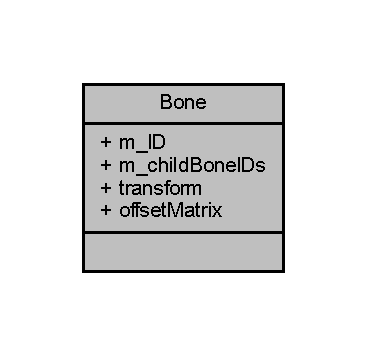
\includegraphics[width=176pt]{struct_bone__coll__graph}
\end{center}
\end{figure}
\subsection*{Public Attributes}
\begin{DoxyCompactItemize}
\item 
int \hyperlink{struct_bone_ae27ac3ac39d8e707ba29f09a073564da}{m\+\_\+\+ID}
\item 
std\+::vector$<$ int $>$ \hyperlink{struct_bone_a00052ee6d532b058efa699b9b21e61f2}{m\+\_\+child\+Bone\+I\+Ds}
\item 
\hyperlink{_types_8h_a2db59f395fe82a7394c6324956c265d8}{mat4} \hyperlink{struct_bone_a24c5bc5cfeb022d82677b5f786d74ff2}{transform}
\item 
\hyperlink{_types_8h_a2db59f395fe82a7394c6324956c265d8}{mat4} \hyperlink{struct_bone_a842ad02b3b17a412a3fd505081c186db}{offset\+Matrix}
\end{DoxyCompactItemize}


\subsection{Detailed Description}


Definition at line 23 of file Skeleton.\+h.



\subsection{Member Data Documentation}
\index{Bone@{Bone}!m\+\_\+child\+Bone\+I\+Ds@{m\+\_\+child\+Bone\+I\+Ds}}
\index{m\+\_\+child\+Bone\+I\+Ds@{m\+\_\+child\+Bone\+I\+Ds}!Bone@{Bone}}
\subsubsection[{\texorpdfstring{m\+\_\+child\+Bone\+I\+Ds}{m_childBoneIDs}}]{\setlength{\rightskip}{0pt plus 5cm}std\+::vector$<$int$>$ Bone\+::m\+\_\+child\+Bone\+I\+Ds}\hypertarget{struct_bone_a00052ee6d532b058efa699b9b21e61f2}{}\label{struct_bone_a00052ee6d532b058efa699b9b21e61f2}


Definition at line 26 of file Skeleton.\+h.

\index{Bone@{Bone}!m\+\_\+\+ID@{m\+\_\+\+ID}}
\index{m\+\_\+\+ID@{m\+\_\+\+ID}!Bone@{Bone}}
\subsubsection[{\texorpdfstring{m\+\_\+\+ID}{m_ID}}]{\setlength{\rightskip}{0pt plus 5cm}int Bone\+::m\+\_\+\+ID}\hypertarget{struct_bone_ae27ac3ac39d8e707ba29f09a073564da}{}\label{struct_bone_ae27ac3ac39d8e707ba29f09a073564da}


Definition at line 25 of file Skeleton.\+h.

\index{Bone@{Bone}!offset\+Matrix@{offset\+Matrix}}
\index{offset\+Matrix@{offset\+Matrix}!Bone@{Bone}}
\subsubsection[{\texorpdfstring{offset\+Matrix}{offsetMatrix}}]{\setlength{\rightskip}{0pt plus 5cm}{\bf mat4} Bone\+::offset\+Matrix}\hypertarget{struct_bone_a842ad02b3b17a412a3fd505081c186db}{}\label{struct_bone_a842ad02b3b17a412a3fd505081c186db}


Definition at line 28 of file Skeleton.\+h.

\index{Bone@{Bone}!transform@{transform}}
\index{transform@{transform}!Bone@{Bone}}
\subsubsection[{\texorpdfstring{transform}{transform}}]{\setlength{\rightskip}{0pt plus 5cm}{\bf mat4} Bone\+::transform}\hypertarget{struct_bone_a24c5bc5cfeb022d82677b5f786d74ff2}{}\label{struct_bone_a24c5bc5cfeb022d82677b5f786d74ff2}


Definition at line 27 of file Skeleton.\+h.



Referenced by Skeleton\+::\+Calculate\+Bone\+Transforms().



The documentation for this struct was generated from the following file\+:\begin{DoxyCompactItemize}
\item 
C\+:/\+Users/elizabeth/\+Documents/\+Git\+Hub/\+Engine/\+Open\+G\+L\+Engine/\+Open\+G\+L\+Engine/\hyperlink{_skeleton_8h}{Skeleton.\+h}\end{DoxyCompactItemize}

\hypertarget{class_bone_key_sequence}{}\section{Bone\+Key\+Sequence Class Reference}
\label{class_bone_key_sequence}\index{Bone\+Key\+Sequence@{Bone\+Key\+Sequence}}


{\ttfamily \#include $<$Bone\+Key\+Sequence.\+h$>$}



Collaboration diagram for Bone\+Key\+Sequence\+:\nopagebreak
\begin{figure}[H]
\begin{center}
\leavevmode
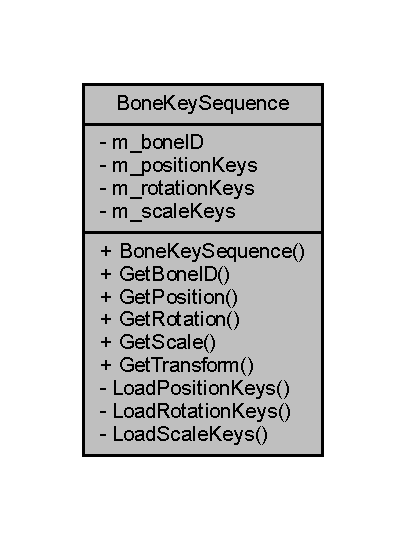
\includegraphics[width=195pt]{class_bone_key_sequence__coll__graph}
\end{center}
\end{figure}
\subsection*{Public Member Functions}
\begin{DoxyCompactItemize}
\item 
\hyperlink{class_bone_key_sequence_ad186adb564fba0e3d87286c3f78f3ec2}{Bone\+Key\+Sequence} (ai\+Node\+Anim const $\ast$p\+Anim, int bone\+ID)
\begin{DoxyCompactList}\small\item\em Initializes a new instance of the \hyperlink{class_bone_key_sequence}{Bone\+Key\+Sequence} class. \end{DoxyCompactList}\item 
int \hyperlink{class_bone_key_sequence_ac43149e05d6f297d215a4166fcd6f909}{Get\+Bone\+ID} () const 
\begin{DoxyCompactList}\small\item\em Gets the bone identifier. \end{DoxyCompactList}\item 
\hyperlink{_types_8h_a3d0ce73e3199de81565fb01632415288}{vec3} \hyperlink{class_bone_key_sequence_a88b854b70d320cf1f08ae38ea156f3e1}{Get\+Position} (float time) const 
\begin{DoxyCompactList}\small\item\em Gets the position. \end{DoxyCompactList}\item 
\hyperlink{_types_8h_a02abcac728eae225e929e9e0dc427f28}{quat} \hyperlink{class_bone_key_sequence_aae8845be8d37c41e0e61bc27d07354f2}{Get\+Rotation} (float time) const 
\begin{DoxyCompactList}\small\item\em Gets the rotation. \end{DoxyCompactList}\item 
\hyperlink{_types_8h_a3d0ce73e3199de81565fb01632415288}{vec3} \hyperlink{class_bone_key_sequence_a54a036ab5a976bb00d3c470281ab65f1}{Get\+Scale} (float time) const 
\begin{DoxyCompactList}\small\item\em Gets the scale. \end{DoxyCompactList}\item 
\hyperlink{_types_8h_a2db59f395fe82a7394c6324956c265d8}{mat4} \hyperlink{class_bone_key_sequence_acec08fe52251082ea3d224189f7cf201}{Get\+Transform} (float time) const 
\begin{DoxyCompactList}\small\item\em Gets the transform. \end{DoxyCompactList}\end{DoxyCompactItemize}
\subsection*{Private Member Functions}
\begin{DoxyCompactItemize}
\item 
void \hyperlink{class_bone_key_sequence_a9165c4e680ccb15818a1f895e7445332}{Load\+Position\+Keys} (ai\+Node\+Anim const $\ast$p\+Anim)
\begin{DoxyCompactList}\small\item\em Loads the position keys. \end{DoxyCompactList}\item 
void \hyperlink{class_bone_key_sequence_a9eebce05ff9c1a59187f9f8d31fc6f49}{Load\+Rotation\+Keys} (ai\+Node\+Anim const $\ast$p\+Anim)
\begin{DoxyCompactList}\small\item\em Loads the rotation keys. \end{DoxyCompactList}\item 
void \hyperlink{class_bone_key_sequence_af6d9f85bb507d3712d9805b3a5a05421}{Load\+Scale\+Keys} (ai\+Node\+Anim const $\ast$p\+Anim)
\begin{DoxyCompactList}\small\item\em Loads the scale keys. \end{DoxyCompactList}\end{DoxyCompactItemize}
\subsection*{Private Attributes}
\begin{DoxyCompactItemize}
\item 
int \hyperlink{class_bone_key_sequence_a3479ae87f50df83ca145080406a1c3b8}{m\+\_\+bone\+ID}
\begin{DoxyCompactList}\small\item\em The bone identifier \end{DoxyCompactList}\item 
std\+::vector$<$ \hyperlink{struct_position_key}{Position\+Key} $>$ \hyperlink{class_bone_key_sequence_acae9becd7de02c955da5d64050513ce5}{m\+\_\+position\+Keys}
\begin{DoxyCompactList}\small\item\em The position keys \end{DoxyCompactList}\item 
std\+::vector$<$ \hyperlink{struct_rotation_key}{Rotation\+Key} $>$ \hyperlink{class_bone_key_sequence_abb6be9db9c5bdc089b6ae7ea6bdae0e3}{m\+\_\+rotation\+Keys}
\begin{DoxyCompactList}\small\item\em The rotation keys \end{DoxyCompactList}\item 
std\+::vector$<$ \hyperlink{struct_scale_key}{Scale\+Key} $>$ \hyperlink{class_bone_key_sequence_a9a1a5986127adf2f67411d8802463c36}{m\+\_\+scale\+Keys}
\begin{DoxyCompactList}\small\item\em The scale keys \end{DoxyCompactList}\end{DoxyCompactItemize}


\subsection{Detailed Description}


Definition at line 36 of file Bone\+Key\+Sequence.\+h.



\subsection{Constructor \& Destructor Documentation}
\index{Bone\+Key\+Sequence@{Bone\+Key\+Sequence}!Bone\+Key\+Sequence@{Bone\+Key\+Sequence}}
\index{Bone\+Key\+Sequence@{Bone\+Key\+Sequence}!Bone\+Key\+Sequence@{Bone\+Key\+Sequence}}
\subsubsection[{\texorpdfstring{Bone\+Key\+Sequence(ai\+Node\+Anim const $\ast$p\+Anim, int bone\+I\+D)}{BoneKeySequence(aiNodeAnim const *pAnim, int boneID)}}]{\setlength{\rightskip}{0pt plus 5cm}Bone\+Key\+Sequence\+::\+Bone\+Key\+Sequence (
\begin{DoxyParamCaption}
\item[{ai\+Node\+Anim const $\ast$}]{p\+Anim, }
\item[{int}]{bone\+ID}
\end{DoxyParamCaption}
)}\hypertarget{class_bone_key_sequence_ad186adb564fba0e3d87286c3f78f3ec2}{}\label{class_bone_key_sequence_ad186adb564fba0e3d87286c3f78f3ec2}


Initializes a new instance of the \hyperlink{class_bone_key_sequence}{Bone\+Key\+Sequence} class. 


\begin{DoxyParams}{Parameters}
{\em p\+Anim} & The p anim.\\
\hline
{\em bone\+ID} & The bone identifier.\\
\hline
\end{DoxyParams}


Definition at line 6 of file Bone\+Key\+Sequence.\+cpp.



References Load\+Position\+Keys(), Load\+Rotation\+Keys(), Load\+Scale\+Keys(), and m\+\_\+bone\+ID.


\begin{DoxyCode}
7   : \hyperlink{class_bone_key_sequence_a3479ae87f50df83ca145080406a1c3b8}{m\_boneID}(boneID)
8 \{
9   \hyperlink{class_bone_key_sequence_a9165c4e680ccb15818a1f895e7445332}{LoadPositionKeys}(pAnim);
10   \hyperlink{class_bone_key_sequence_a9eebce05ff9c1a59187f9f8d31fc6f49}{LoadRotationKeys}(pAnim);
11   \hyperlink{class_bone_key_sequence_af6d9f85bb507d3712d9805b3a5a05421}{LoadScaleKeys}(pAnim);
12 \}
\end{DoxyCode}


Here is the call graph for this function\+:\nopagebreak
\begin{figure}[H]
\begin{center}
\leavevmode
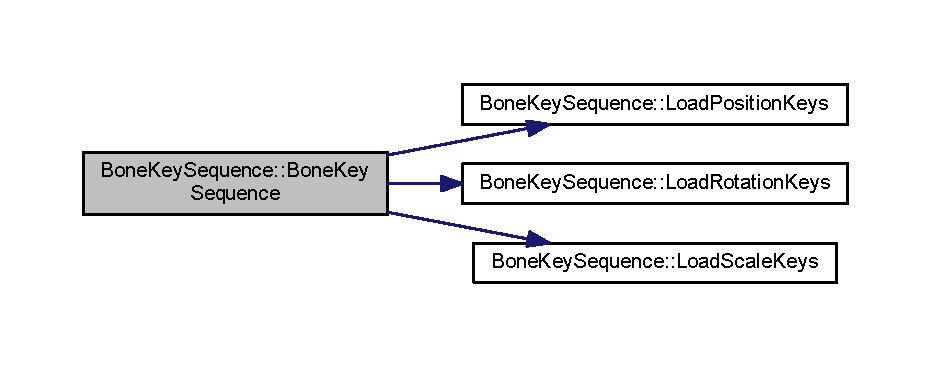
\includegraphics[width=350pt]{class_bone_key_sequence_ad186adb564fba0e3d87286c3f78f3ec2_cgraph}
\end{center}
\end{figure}




\subsection{Member Function Documentation}
\index{Bone\+Key\+Sequence@{Bone\+Key\+Sequence}!Get\+Bone\+ID@{Get\+Bone\+ID}}
\index{Get\+Bone\+ID@{Get\+Bone\+ID}!Bone\+Key\+Sequence@{Bone\+Key\+Sequence}}
\subsubsection[{\texorpdfstring{Get\+Bone\+I\+D() const }{GetBoneID() const }}]{\setlength{\rightskip}{0pt plus 5cm}int Bone\+Key\+Sequence\+::\+Get\+Bone\+ID (
\begin{DoxyParamCaption}
{}
\end{DoxyParamCaption}
) const}\hypertarget{class_bone_key_sequence_ac43149e05d6f297d215a4166fcd6f909}{}\label{class_bone_key_sequence_ac43149e05d6f297d215a4166fcd6f909}


Gets the bone identifier. 

\begin{DoxyReturn}{Returns}
int
\end{DoxyReturn}


Definition at line 14 of file Bone\+Key\+Sequence.\+cpp.



References m\+\_\+bone\+ID.


\begin{DoxyCode}
15 \{
16   \textcolor{keywordflow}{return} \hyperlink{class_bone_key_sequence_a3479ae87f50df83ca145080406a1c3b8}{m\_boneID};
17 \}
\end{DoxyCode}
\index{Bone\+Key\+Sequence@{Bone\+Key\+Sequence}!Get\+Position@{Get\+Position}}
\index{Get\+Position@{Get\+Position}!Bone\+Key\+Sequence@{Bone\+Key\+Sequence}}
\subsubsection[{\texorpdfstring{Get\+Position(float time) const }{GetPosition(float time) const }}]{\setlength{\rightskip}{0pt plus 5cm}{\bf vec3} Bone\+Key\+Sequence\+::\+Get\+Position (
\begin{DoxyParamCaption}
\item[{float}]{time}
\end{DoxyParamCaption}
) const}\hypertarget{class_bone_key_sequence_a88b854b70d320cf1f08ae38ea156f3e1}{}\label{class_bone_key_sequence_a88b854b70d320cf1f08ae38ea156f3e1}


Gets the position. 


\begin{DoxyParams}{Parameters}
{\em time} & The time.\\
\hline
\end{DoxyParams}
\begin{DoxyReturn}{Returns}
vec3
\end{DoxyReturn}


Definition at line 19 of file Bone\+Key\+Sequence.\+cpp.



References Position\+Key\+::time.



Referenced by Get\+Transform().


\begin{DoxyCode}
20 \{
21   \textcolor{keywordflow}{if} (time <= \hyperlink{class_bone_key_sequence_acae9becd7de02c955da5d64050513ce5}{m\_positionKeys}[0].time)
22     \textcolor{keywordflow}{return} \hyperlink{class_bone_key_sequence_acae9becd7de02c955da5d64050513ce5}{m\_positionKeys}[0].position;
23 
24   \textcolor{keywordflow}{if} (time >= \hyperlink{class_bone_key_sequence_acae9becd7de02c955da5d64050513ce5}{m\_positionKeys}[\hyperlink{class_bone_key_sequence_acae9becd7de02c955da5d64050513ce5}{m\_positionKeys}.size() - 1].time)
25     \textcolor{keywordflow}{return} \hyperlink{class_bone_key_sequence_acae9becd7de02c955da5d64050513ce5}{m\_positionKeys}[\hyperlink{class_bone_key_sequence_acae9becd7de02c955da5d64050513ce5}{m\_positionKeys}.size() - 1].position;
26 
27   \textcolor{comment}{//Find last frame before the current time}
28   \textcolor{keywordtype}{int} lastFrameIndex = 0;
29   \textcolor{keywordflow}{for} (\textcolor{keywordtype}{int} i = 1; i < \hyperlink{class_bone_key_sequence_acae9becd7de02c955da5d64050513ce5}{m\_positionKeys}.size(); i++)
30     \textcolor{keywordflow}{if} (\hyperlink{class_bone_key_sequence_acae9becd7de02c955da5d64050513ce5}{m\_positionKeys}[i].time < time)
31       lastFrameIndex = i;
32     \textcolor{keywordflow}{else}
33       \textcolor{keywordflow}{break};
34 
35   \hyperlink{struct_position_key}{PositionKey} \textcolor{keyword}{const}& lastKey = \hyperlink{class_bone_key_sequence_acae9becd7de02c955da5d64050513ce5}{m\_positionKeys}[lastFrameIndex];
36   \hyperlink{struct_position_key}{PositionKey} \textcolor{keyword}{const}& nextKey = \hyperlink{class_bone_key_sequence_acae9becd7de02c955da5d64050513ce5}{m\_positionKeys}[lastFrameIndex + 1];
37   
38   \textcolor{keywordtype}{float} timeSinceLast = time - lastKey.\hyperlink{struct_position_key_ab18d1c0baf9f835e2dbd8b8663d552f4}{time};
39   \textcolor{keywordtype}{float} timeBetweenFrames = nextKey.\hyperlink{struct_position_key_ab18d1c0baf9f835e2dbd8b8663d552f4}{time} - lastKey.\hyperlink{struct_position_key_ab18d1c0baf9f835e2dbd8b8663d552f4}{time};
40   \textcolor{keywordtype}{float} interpolationFactor = timeSinceLast / timeBetweenFrames;
41   interpolationFactor = \hyperlink{_m_math_8h_a35bcf6994210feb2d96d1d22df3385ea}{mClamp}(interpolationFactor, 0, 1);
42   
43   \textcolor{keywordflow}{return} glm::lerp(lastKey.\hyperlink{struct_position_key_a6b7f3212adb099bc1b5d86513ef2fd36}{position}, nextKey.\hyperlink{struct_position_key_a6b7f3212adb099bc1b5d86513ef2fd36}{position}, interpolationFactor);
44 \}
\end{DoxyCode}


Here is the caller graph for this function\+:\nopagebreak
\begin{figure}[H]
\begin{center}
\leavevmode
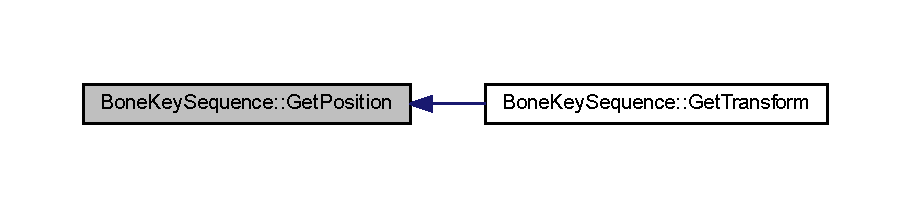
\includegraphics[width=350pt]{class_bone_key_sequence_a88b854b70d320cf1f08ae38ea156f3e1_icgraph}
\end{center}
\end{figure}


\index{Bone\+Key\+Sequence@{Bone\+Key\+Sequence}!Get\+Rotation@{Get\+Rotation}}
\index{Get\+Rotation@{Get\+Rotation}!Bone\+Key\+Sequence@{Bone\+Key\+Sequence}}
\subsubsection[{\texorpdfstring{Get\+Rotation(float time) const }{GetRotation(float time) const }}]{\setlength{\rightskip}{0pt plus 5cm}{\bf quat} Bone\+Key\+Sequence\+::\+Get\+Rotation (
\begin{DoxyParamCaption}
\item[{float}]{time}
\end{DoxyParamCaption}
) const}\hypertarget{class_bone_key_sequence_aae8845be8d37c41e0e61bc27d07354f2}{}\label{class_bone_key_sequence_aae8845be8d37c41e0e61bc27d07354f2}


Gets the rotation. 


\begin{DoxyParams}{Parameters}
{\em time} & The time.\\
\hline
\end{DoxyParams}
\begin{DoxyReturn}{Returns}
quat
\end{DoxyReturn}


Definition at line 46 of file Bone\+Key\+Sequence.\+cpp.



References Rotation\+Key\+::time.



Referenced by Get\+Transform().


\begin{DoxyCode}
47 \{
48   \textcolor{keywordflow}{if} (time <= \hyperlink{class_bone_key_sequence_abb6be9db9c5bdc089b6ae7ea6bdae0e3}{m\_rotationKeys}[0].time)
49     \textcolor{keywordflow}{return} \hyperlink{class_bone_key_sequence_abb6be9db9c5bdc089b6ae7ea6bdae0e3}{m\_rotationKeys}[0].rotation;
50 
51   \textcolor{keywordflow}{if} (time >= \hyperlink{class_bone_key_sequence_abb6be9db9c5bdc089b6ae7ea6bdae0e3}{m\_rotationKeys}[\hyperlink{class_bone_key_sequence_abb6be9db9c5bdc089b6ae7ea6bdae0e3}{m\_rotationKeys}.size() - 1].time)
52     \textcolor{keywordflow}{return} \hyperlink{class_bone_key_sequence_abb6be9db9c5bdc089b6ae7ea6bdae0e3}{m\_rotationKeys}[\hyperlink{class_bone_key_sequence_abb6be9db9c5bdc089b6ae7ea6bdae0e3}{m\_rotationKeys}.size() - 1].rotation;
53 
54   \textcolor{comment}{//Find last frame before the current time}
55   \textcolor{keywordtype}{int} lastFrameIndex = 0;
56   \textcolor{keywordflow}{for} (\textcolor{keywordtype}{int} i = 1; i < \hyperlink{class_bone_key_sequence_abb6be9db9c5bdc089b6ae7ea6bdae0e3}{m\_rotationKeys}.size(); i++)
57     \textcolor{keywordflow}{if} (\hyperlink{class_bone_key_sequence_abb6be9db9c5bdc089b6ae7ea6bdae0e3}{m\_rotationKeys}[i].time < time)
58       lastFrameIndex = i;
59     \textcolor{keywordflow}{else}
60       \textcolor{keywordflow}{break};
61 
62   \hyperlink{struct_rotation_key}{RotationKey} \textcolor{keyword}{const}& lastKey = \hyperlink{class_bone_key_sequence_abb6be9db9c5bdc089b6ae7ea6bdae0e3}{m\_rotationKeys}[lastFrameIndex];
63   \hyperlink{struct_rotation_key}{RotationKey} \textcolor{keyword}{const}& nextKey = \hyperlink{class_bone_key_sequence_abb6be9db9c5bdc089b6ae7ea6bdae0e3}{m\_rotationKeys}[lastFrameIndex + 1];
64 
65   \textcolor{keywordtype}{float} timeSinceLast = time - lastKey.\hyperlink{struct_rotation_key_a421ab28d247b062e4c46e4879943ee7d}{time};
66   \textcolor{keywordtype}{float} timeBetweenFrames = nextKey.\hyperlink{struct_rotation_key_a421ab28d247b062e4c46e4879943ee7d}{time} - lastKey.\hyperlink{struct_rotation_key_a421ab28d247b062e4c46e4879943ee7d}{time};
67   \textcolor{keywordtype}{float} interpolationFactor = timeSinceLast / timeBetweenFrames;
68   interpolationFactor = \hyperlink{_m_math_8h_a35bcf6994210feb2d96d1d22df3385ea}{mClamp}(interpolationFactor, 0, 1);
69 
70   \textcolor{keywordflow}{return} glm::lerp(lastKey.\hyperlink{struct_rotation_key_a9638fbf119b41fd844b3d24c9e95d52d}{rotation}, nextKey.\hyperlink{struct_rotation_key_a9638fbf119b41fd844b3d24c9e95d52d}{rotation}, interpolationFactor);
71 \}
\end{DoxyCode}


Here is the caller graph for this function\+:\nopagebreak
\begin{figure}[H]
\begin{center}
\leavevmode
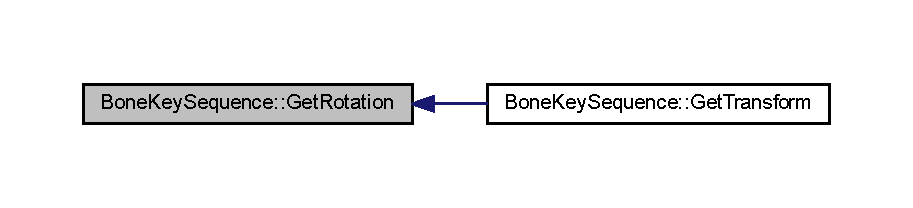
\includegraphics[width=350pt]{class_bone_key_sequence_aae8845be8d37c41e0e61bc27d07354f2_icgraph}
\end{center}
\end{figure}


\index{Bone\+Key\+Sequence@{Bone\+Key\+Sequence}!Get\+Scale@{Get\+Scale}}
\index{Get\+Scale@{Get\+Scale}!Bone\+Key\+Sequence@{Bone\+Key\+Sequence}}
\subsubsection[{\texorpdfstring{Get\+Scale(float time) const }{GetScale(float time) const }}]{\setlength{\rightskip}{0pt plus 5cm}{\bf vec3} Bone\+Key\+Sequence\+::\+Get\+Scale (
\begin{DoxyParamCaption}
\item[{float}]{time}
\end{DoxyParamCaption}
) const}\hypertarget{class_bone_key_sequence_a54a036ab5a976bb00d3c470281ab65f1}{}\label{class_bone_key_sequence_a54a036ab5a976bb00d3c470281ab65f1}


Gets the scale. 


\begin{DoxyParams}{Parameters}
{\em time} & The time.\\
\hline
\end{DoxyParams}
\begin{DoxyReturn}{Returns}
vec3
\end{DoxyReturn}


Definition at line 73 of file Bone\+Key\+Sequence.\+cpp.



References Scale\+Key\+::time.



Referenced by Get\+Transform().


\begin{DoxyCode}
74 \{
75   \textcolor{keywordflow}{if} (time <= \hyperlink{class_bone_key_sequence_a9a1a5986127adf2f67411d8802463c36}{m\_scaleKeys}[0].time)
76     \textcolor{keywordflow}{return} \hyperlink{class_bone_key_sequence_a9a1a5986127adf2f67411d8802463c36}{m\_scaleKeys}[0].scale;
77 
78   \textcolor{keywordflow}{if} (time >= \hyperlink{class_bone_key_sequence_a9a1a5986127adf2f67411d8802463c36}{m\_scaleKeys}[\hyperlink{class_bone_key_sequence_a9a1a5986127adf2f67411d8802463c36}{m\_scaleKeys}.size() - 1].time)
79     \textcolor{keywordflow}{return} \hyperlink{class_bone_key_sequence_a9a1a5986127adf2f67411d8802463c36}{m\_scaleKeys}[\hyperlink{class_bone_key_sequence_a9a1a5986127adf2f67411d8802463c36}{m\_scaleKeys}.size() - 1].scale;
80 
81   \textcolor{comment}{//Find last frame before the current time}
82   \textcolor{keywordtype}{int} lastFrameIndex = 0;
83   \textcolor{keywordflow}{for} (\textcolor{keywordtype}{int} i = 1; i < \hyperlink{class_bone_key_sequence_a9a1a5986127adf2f67411d8802463c36}{m\_scaleKeys}.size(); i++)
84     \textcolor{keywordflow}{if} (\hyperlink{class_bone_key_sequence_a9a1a5986127adf2f67411d8802463c36}{m\_scaleKeys}[i].time < time)
85       lastFrameIndex = i;
86     \textcolor{keywordflow}{else}
87       \textcolor{keywordflow}{break};
88 
89   \hyperlink{struct_scale_key}{ScaleKey} \textcolor{keyword}{const}& lastKey = \hyperlink{class_bone_key_sequence_a9a1a5986127adf2f67411d8802463c36}{m\_scaleKeys}[lastFrameIndex];
90   \hyperlink{struct_scale_key}{ScaleKey} \textcolor{keyword}{const}& nextKey = \hyperlink{class_bone_key_sequence_a9a1a5986127adf2f67411d8802463c36}{m\_scaleKeys}[lastFrameIndex + 1];
91 
92   \textcolor{keywordtype}{float} timeSinceLast = time - lastKey.\hyperlink{struct_scale_key_a5fc8b5f2ab58d62addddbb51a794fee7}{time};
93   \textcolor{keywordtype}{float} timeBetweenFrames = nextKey.\hyperlink{struct_scale_key_a5fc8b5f2ab58d62addddbb51a794fee7}{time} - lastKey.\hyperlink{struct_scale_key_a5fc8b5f2ab58d62addddbb51a794fee7}{time};
94   \textcolor{keywordtype}{float} interpolationFactor = timeSinceLast / timeBetweenFrames;
95   interpolationFactor = \hyperlink{_m_math_8h_a35bcf6994210feb2d96d1d22df3385ea}{mClamp}(interpolationFactor, 0, 1);
96 
97   \textcolor{keywordflow}{return} glm::lerp(lastKey.\hyperlink{struct_scale_key_a49c1e61733ade0134fb94a62620d2caf}{scale}, nextKey.\hyperlink{struct_scale_key_a49c1e61733ade0134fb94a62620d2caf}{scale}, interpolationFactor);
98 \}
\end{DoxyCode}


Here is the caller graph for this function\+:\nopagebreak
\begin{figure}[H]
\begin{center}
\leavevmode
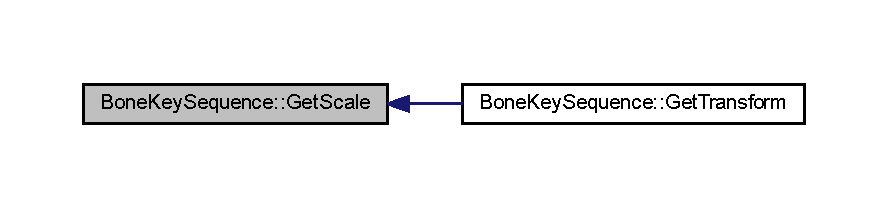
\includegraphics[width=350pt]{class_bone_key_sequence_a54a036ab5a976bb00d3c470281ab65f1_icgraph}
\end{center}
\end{figure}


\index{Bone\+Key\+Sequence@{Bone\+Key\+Sequence}!Get\+Transform@{Get\+Transform}}
\index{Get\+Transform@{Get\+Transform}!Bone\+Key\+Sequence@{Bone\+Key\+Sequence}}
\subsubsection[{\texorpdfstring{Get\+Transform(float time) const }{GetTransform(float time) const }}]{\setlength{\rightskip}{0pt plus 5cm}{\bf mat4} Bone\+Key\+Sequence\+::\+Get\+Transform (
\begin{DoxyParamCaption}
\item[{float}]{time}
\end{DoxyParamCaption}
) const}\hypertarget{class_bone_key_sequence_acec08fe52251082ea3d224189f7cf201}{}\label{class_bone_key_sequence_acec08fe52251082ea3d224189f7cf201}


Gets the transform. 


\begin{DoxyParams}{Parameters}
{\em time} & The time.\\
\hline
\end{DoxyParams}
\begin{DoxyReturn}{Returns}
mat4
\end{DoxyReturn}


Definition at line 100 of file Bone\+Key\+Sequence.\+cpp.



References Get\+Position(), Get\+Rotation(), and Get\+Scale().


\begin{DoxyCode}
101 \{
102   \hyperlink{_types_8h_a3d0ce73e3199de81565fb01632415288}{vec3} position = \hyperlink{class_bone_key_sequence_a88b854b70d320cf1f08ae38ea156f3e1}{GetPosition}(time);
103   \hyperlink{_types_8h_a3d0ce73e3199de81565fb01632415288}{vec3} scale = \hyperlink{class_bone_key_sequence_a54a036ab5a976bb00d3c470281ab65f1}{GetScale}(time);
104   \hyperlink{_types_8h_a02abcac728eae225e929e9e0dc427f28}{quat} rotation = \hyperlink{class_bone_key_sequence_aae8845be8d37c41e0e61bc27d07354f2}{GetRotation}(time);
105 
106   \hyperlink{_types_8h_a2db59f395fe82a7394c6324956c265d8}{mat4} translationMatrix = glm::translate(position);
107   \hyperlink{_types_8h_a2db59f395fe82a7394c6324956c265d8}{mat4} scalingMatrix = glm::scale(scale);
108   \hyperlink{_types_8h_a2db59f395fe82a7394c6324956c265d8}{mat4} rotationMatrix = \hyperlink{_types_8h_a2db59f395fe82a7394c6324956c265d8}{mat4}(rotation);
109 
110   \textcolor{keywordflow}{return} translationMatrix * rotationMatrix * scalingMatrix;
111 \}
\end{DoxyCode}


Here is the call graph for this function\+:\nopagebreak
\begin{figure}[H]
\begin{center}
\leavevmode
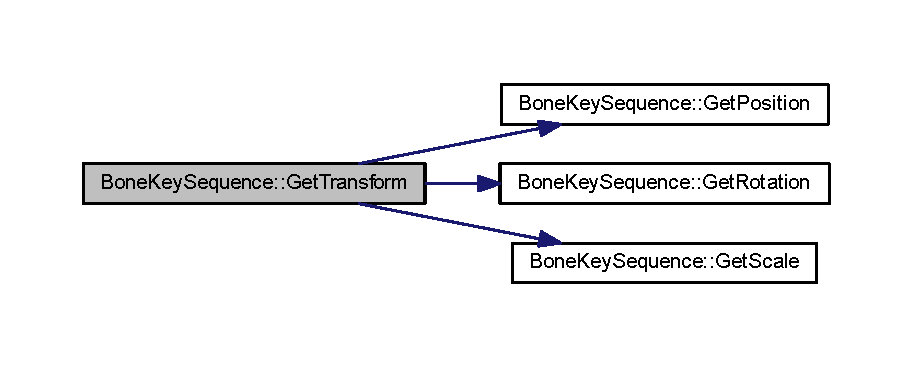
\includegraphics[width=350pt]{class_bone_key_sequence_acec08fe52251082ea3d224189f7cf201_cgraph}
\end{center}
\end{figure}


\index{Bone\+Key\+Sequence@{Bone\+Key\+Sequence}!Load\+Position\+Keys@{Load\+Position\+Keys}}
\index{Load\+Position\+Keys@{Load\+Position\+Keys}!Bone\+Key\+Sequence@{Bone\+Key\+Sequence}}
\subsubsection[{\texorpdfstring{Load\+Position\+Keys(ai\+Node\+Anim const $\ast$p\+Anim)}{LoadPositionKeys(aiNodeAnim const *pAnim)}}]{\setlength{\rightskip}{0pt plus 5cm}void Bone\+Key\+Sequence\+::\+Load\+Position\+Keys (
\begin{DoxyParamCaption}
\item[{ai\+Node\+Anim const $\ast$}]{p\+Anim}
\end{DoxyParamCaption}
)\hspace{0.3cm}{\ttfamily [private]}}\hypertarget{class_bone_key_sequence_a9165c4e680ccb15818a1f895e7445332}{}\label{class_bone_key_sequence_a9165c4e680ccb15818a1f895e7445332}


Loads the position keys. 


\begin{DoxyParams}{Parameters}
{\em p\+Anim} & The p anim.\\
\hline
\end{DoxyParams}


Definition at line 113 of file Bone\+Key\+Sequence.\+cpp.



Referenced by Bone\+Key\+Sequence().


\begin{DoxyCode}
114 \{
115   \textcolor{keywordflow}{for} (\hyperlink{_types_8h_a4f5fce8c1ef282264f9214809524d836}{uint} i = 0; i < pAnim->mNumPositionKeys; i++)
116       \hyperlink{class_bone_key_sequence_acae9becd7de02c955da5d64050513ce5}{m\_positionKeys}.push\_back(\hyperlink{struct_position_key}{PositionKey}\{ float(pAnim->mPositionKeys[i].mTime), 
      ASToGLM(pAnim->mPositionKeys[i].mValue) \});
117 \}
\end{DoxyCode}


Here is the caller graph for this function\+:\nopagebreak
\begin{figure}[H]
\begin{center}
\leavevmode
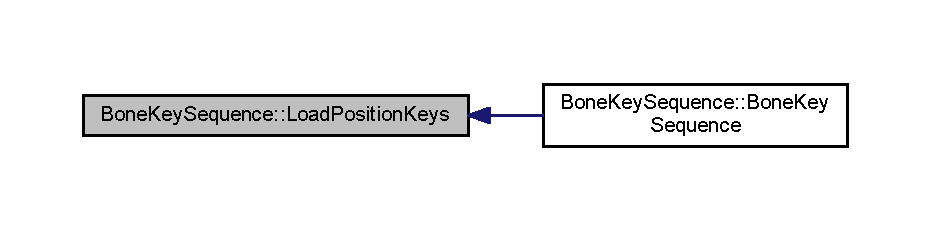
\includegraphics[width=350pt]{class_bone_key_sequence_a9165c4e680ccb15818a1f895e7445332_icgraph}
\end{center}
\end{figure}


\index{Bone\+Key\+Sequence@{Bone\+Key\+Sequence}!Load\+Rotation\+Keys@{Load\+Rotation\+Keys}}
\index{Load\+Rotation\+Keys@{Load\+Rotation\+Keys}!Bone\+Key\+Sequence@{Bone\+Key\+Sequence}}
\subsubsection[{\texorpdfstring{Load\+Rotation\+Keys(ai\+Node\+Anim const $\ast$p\+Anim)}{LoadRotationKeys(aiNodeAnim const *pAnim)}}]{\setlength{\rightskip}{0pt plus 5cm}void Bone\+Key\+Sequence\+::\+Load\+Rotation\+Keys (
\begin{DoxyParamCaption}
\item[{ai\+Node\+Anim const $\ast$}]{p\+Anim}
\end{DoxyParamCaption}
)\hspace{0.3cm}{\ttfamily [private]}}\hypertarget{class_bone_key_sequence_a9eebce05ff9c1a59187f9f8d31fc6f49}{}\label{class_bone_key_sequence_a9eebce05ff9c1a59187f9f8d31fc6f49}


Loads the rotation keys. 


\begin{DoxyParams}{Parameters}
{\em p\+Anim} & The p anim.\\
\hline
\end{DoxyParams}


Definition at line 119 of file Bone\+Key\+Sequence.\+cpp.



Referenced by Bone\+Key\+Sequence().


\begin{DoxyCode}
120 \{
121   \textcolor{keywordflow}{for} (\hyperlink{_types_8h_a4f5fce8c1ef282264f9214809524d836}{uint} i = 0; i < pAnim->mNumRotationKeys; i++)
122       \hyperlink{class_bone_key_sequence_abb6be9db9c5bdc089b6ae7ea6bdae0e3}{m\_rotationKeys}.push\_back(\hyperlink{struct_rotation_key}{RotationKey}\{ float(pAnim->mRotationKeys[i].mTime), 
      ASToGLM(pAnim->mRotationKeys[i].mValue) \});
123 \}
\end{DoxyCode}


Here is the caller graph for this function\+:\nopagebreak
\begin{figure}[H]
\begin{center}
\leavevmode
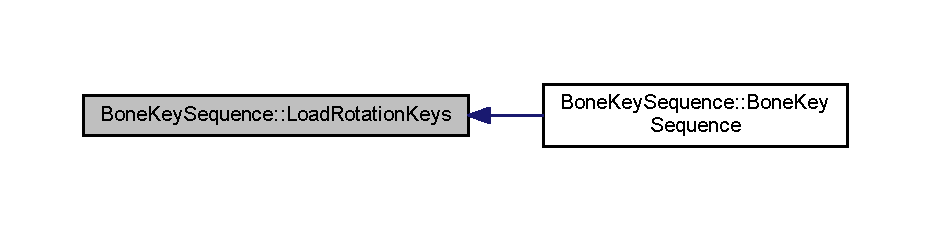
\includegraphics[width=350pt]{class_bone_key_sequence_a9eebce05ff9c1a59187f9f8d31fc6f49_icgraph}
\end{center}
\end{figure}


\index{Bone\+Key\+Sequence@{Bone\+Key\+Sequence}!Load\+Scale\+Keys@{Load\+Scale\+Keys}}
\index{Load\+Scale\+Keys@{Load\+Scale\+Keys}!Bone\+Key\+Sequence@{Bone\+Key\+Sequence}}
\subsubsection[{\texorpdfstring{Load\+Scale\+Keys(ai\+Node\+Anim const $\ast$p\+Anim)}{LoadScaleKeys(aiNodeAnim const *pAnim)}}]{\setlength{\rightskip}{0pt plus 5cm}void Bone\+Key\+Sequence\+::\+Load\+Scale\+Keys (
\begin{DoxyParamCaption}
\item[{ai\+Node\+Anim const $\ast$}]{p\+Anim}
\end{DoxyParamCaption}
)\hspace{0.3cm}{\ttfamily [private]}}\hypertarget{class_bone_key_sequence_af6d9f85bb507d3712d9805b3a5a05421}{}\label{class_bone_key_sequence_af6d9f85bb507d3712d9805b3a5a05421}


Loads the scale keys. 


\begin{DoxyParams}{Parameters}
{\em p\+Anim} & The p anim.\\
\hline
\end{DoxyParams}


Definition at line 125 of file Bone\+Key\+Sequence.\+cpp.



Referenced by Bone\+Key\+Sequence().


\begin{DoxyCode}
126 \{
127   \textcolor{keywordflow}{for} (\hyperlink{_types_8h_a4f5fce8c1ef282264f9214809524d836}{uint} i = 0; i < pAnim->mNumScalingKeys; i++)
128       \hyperlink{class_bone_key_sequence_a9a1a5986127adf2f67411d8802463c36}{m\_scaleKeys}.push\_back(\hyperlink{struct_scale_key}{ScaleKey}\{ float(pAnim->mScalingKeys[i].mTime), ASToGLM(pAnim
      ->mScalingKeys[i].mValue) \});
129 \}\end{DoxyCode}


Here is the caller graph for this function\+:\nopagebreak
\begin{figure}[H]
\begin{center}
\leavevmode
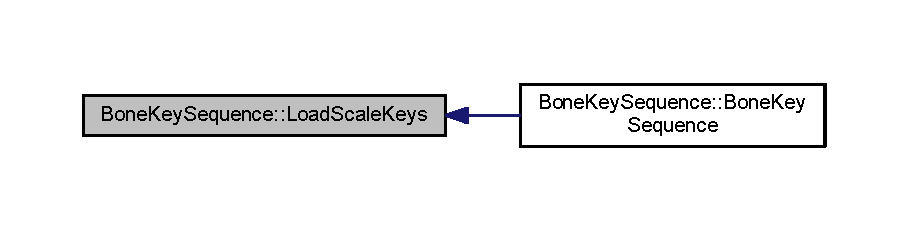
\includegraphics[width=350pt]{class_bone_key_sequence_af6d9f85bb507d3712d9805b3a5a05421_icgraph}
\end{center}
\end{figure}




\subsection{Member Data Documentation}
\index{Bone\+Key\+Sequence@{Bone\+Key\+Sequence}!m\+\_\+bone\+ID@{m\+\_\+bone\+ID}}
\index{m\+\_\+bone\+ID@{m\+\_\+bone\+ID}!Bone\+Key\+Sequence@{Bone\+Key\+Sequence}}
\subsubsection[{\texorpdfstring{m\+\_\+bone\+ID}{m_boneID}}]{\setlength{\rightskip}{0pt plus 5cm}int Bone\+Key\+Sequence\+::m\+\_\+bone\+ID\hspace{0.3cm}{\ttfamily [private]}}\hypertarget{class_bone_key_sequence_a3479ae87f50df83ca145080406a1c3b8}{}\label{class_bone_key_sequence_a3479ae87f50df83ca145080406a1c3b8}


The bone identifier 



Definition at line 88 of file Bone\+Key\+Sequence.\+h.



Referenced by Bone\+Key\+Sequence(), and Get\+Bone\+I\+D().

\index{Bone\+Key\+Sequence@{Bone\+Key\+Sequence}!m\+\_\+position\+Keys@{m\+\_\+position\+Keys}}
\index{m\+\_\+position\+Keys@{m\+\_\+position\+Keys}!Bone\+Key\+Sequence@{Bone\+Key\+Sequence}}
\subsubsection[{\texorpdfstring{m\+\_\+position\+Keys}{m_positionKeys}}]{\setlength{\rightskip}{0pt plus 5cm}std\+::vector$<${\bf Position\+Key}$>$ Bone\+Key\+Sequence\+::m\+\_\+position\+Keys\hspace{0.3cm}{\ttfamily [private]}}\hypertarget{class_bone_key_sequence_acae9becd7de02c955da5d64050513ce5}{}\label{class_bone_key_sequence_acae9becd7de02c955da5d64050513ce5}


The position keys 



Definition at line 93 of file Bone\+Key\+Sequence.\+h.

\index{Bone\+Key\+Sequence@{Bone\+Key\+Sequence}!m\+\_\+rotation\+Keys@{m\+\_\+rotation\+Keys}}
\index{m\+\_\+rotation\+Keys@{m\+\_\+rotation\+Keys}!Bone\+Key\+Sequence@{Bone\+Key\+Sequence}}
\subsubsection[{\texorpdfstring{m\+\_\+rotation\+Keys}{m_rotationKeys}}]{\setlength{\rightskip}{0pt plus 5cm}std\+::vector$<${\bf Rotation\+Key}$>$ Bone\+Key\+Sequence\+::m\+\_\+rotation\+Keys\hspace{0.3cm}{\ttfamily [private]}}\hypertarget{class_bone_key_sequence_abb6be9db9c5bdc089b6ae7ea6bdae0e3}{}\label{class_bone_key_sequence_abb6be9db9c5bdc089b6ae7ea6bdae0e3}


The rotation keys 



Definition at line 98 of file Bone\+Key\+Sequence.\+h.

\index{Bone\+Key\+Sequence@{Bone\+Key\+Sequence}!m\+\_\+scale\+Keys@{m\+\_\+scale\+Keys}}
\index{m\+\_\+scale\+Keys@{m\+\_\+scale\+Keys}!Bone\+Key\+Sequence@{Bone\+Key\+Sequence}}
\subsubsection[{\texorpdfstring{m\+\_\+scale\+Keys}{m_scaleKeys}}]{\setlength{\rightskip}{0pt plus 5cm}std\+::vector$<${\bf Scale\+Key}$>$ Bone\+Key\+Sequence\+::m\+\_\+scale\+Keys\hspace{0.3cm}{\ttfamily [private]}}\hypertarget{class_bone_key_sequence_a9a1a5986127adf2f67411d8802463c36}{}\label{class_bone_key_sequence_a9a1a5986127adf2f67411d8802463c36}


The scale keys 



Definition at line 103 of file Bone\+Key\+Sequence.\+h.



The documentation for this class was generated from the following files\+:\begin{DoxyCompactItemize}
\item 
C\+:/\+Users/elizabeth/\+Documents/\+Git\+Hub/\+Engine/\+Open\+G\+L\+Engine/\+Open\+G\+L\+Engine/\hyperlink{_bone_key_sequence_8h}{Bone\+Key\+Sequence.\+h}\item 
C\+:/\+Users/elizabeth/\+Documents/\+Git\+Hub/\+Engine/\+Open\+G\+L\+Engine/\+Open\+G\+L\+Engine/\hyperlink{_bone_key_sequence_8cpp}{Bone\+Key\+Sequence.\+cpp}\end{DoxyCompactItemize}

\hypertarget{class_camera_a_p_i}{}\section{Camera\+A\+PI Class Reference}
\label{class_camera_a_p_i}\index{Camera\+A\+PI@{Camera\+A\+PI}}


{\ttfamily \#include $<$Camera\+A\+P\+I.\+h$>$}



Collaboration diagram for Camera\+A\+PI\+:\nopagebreak
\begin{figure}[H]
\begin{center}
\leavevmode
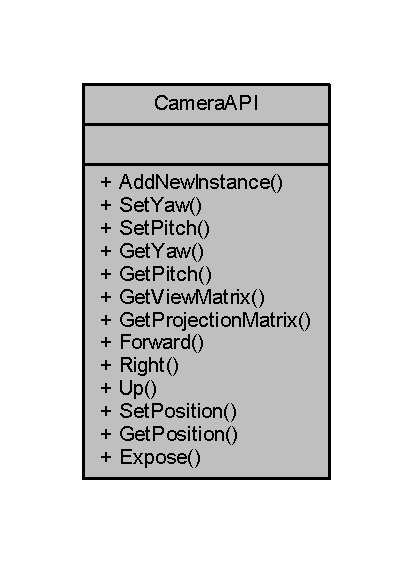
\includegraphics[width=198pt]{class_camera_a_p_i__coll__graph}
\end{center}
\end{figure}
\subsection*{Static Public Member Functions}
\begin{DoxyCompactItemize}
\item 
static \hyperlink{_lua_object_instance_manager_8h_a317edebd09c13058779c942342947a0d}{Instance\+Handle} \hyperlink{class_camera_a_p_i_ad255bd03ff61394e3f9f70ffac703502}{Add\+New\+Instance} ()
\item 
static void \hyperlink{class_camera_a_p_i_a6ae15cbf0c1c5e97645ca6d9b4905b8f}{Set\+Yaw} (\hyperlink{_lua_object_instance_manager_8h_a317edebd09c13058779c942342947a0d}{Instance\+Handle} handle, float yaw)
\item 
static void \hyperlink{class_camera_a_p_i_a1a0543bac7b9bb4edea16ce8c50e8fd8}{Set\+Pitch} (\hyperlink{_lua_object_instance_manager_8h_a317edebd09c13058779c942342947a0d}{Instance\+Handle} handle, float pitch)
\item 
static float \hyperlink{class_camera_a_p_i_a4525769d9d7fc4bd32c5dbd08e195ad4}{Get\+Yaw} (\hyperlink{_lua_object_instance_manager_8h_a317edebd09c13058779c942342947a0d}{Instance\+Handle} handle)
\item 
static float \hyperlink{class_camera_a_p_i_abac2bbe6a37d2fa6d893b6360a9569a5}{Get\+Pitch} (\hyperlink{_lua_object_instance_manager_8h_a317edebd09c13058779c942342947a0d}{Instance\+Handle} handle)
\item 
static \hyperlink{_lua_context_8h_a2220f03700ba40e366f0ee2d684d5c91}{Lua\+Ref} \hyperlink{class_camera_a_p_i_a30cd699e6588dbbf5a993bee609e5c3a}{Get\+View\+Matrix} (\hyperlink{_lua_object_instance_manager_8h_a317edebd09c13058779c942342947a0d}{Instance\+Handle} handle, \hyperlink{_lua_context_8h_a2ffcc2d3ed21165072a1d7b61259bf14}{Lua\+Context\+Handle} context\+Handle)
\item 
static \hyperlink{_lua_context_8h_a2220f03700ba40e366f0ee2d684d5c91}{Lua\+Ref} \hyperlink{class_camera_a_p_i_a122c014eeb4fa24ce1eef7154d1ec934}{Get\+Projection\+Matrix} (\hyperlink{_lua_object_instance_manager_8h_a317edebd09c13058779c942342947a0d}{Instance\+Handle} handle, \hyperlink{_lua_context_8h_a2ffcc2d3ed21165072a1d7b61259bf14}{Lua\+Context\+Handle} context\+Handle)
\item 
static \hyperlink{_lua_context_8h_a2220f03700ba40e366f0ee2d684d5c91}{Lua\+Ref} \hyperlink{class_camera_a_p_i_aaf51389911812005f394aac2c4824a0e}{Forward} (\hyperlink{_lua_object_instance_manager_8h_a317edebd09c13058779c942342947a0d}{Instance\+Handle} handle, \hyperlink{_lua_context_8h_a2ffcc2d3ed21165072a1d7b61259bf14}{Lua\+Context\+Handle} context\+Handle)
\item 
static \hyperlink{_lua_context_8h_a2220f03700ba40e366f0ee2d684d5c91}{Lua\+Ref} \hyperlink{class_camera_a_p_i_aa5880fe8e2c06187a7c2d51eeb84000d}{Right} (\hyperlink{_lua_object_instance_manager_8h_a317edebd09c13058779c942342947a0d}{Instance\+Handle} handle, \hyperlink{_lua_context_8h_a2ffcc2d3ed21165072a1d7b61259bf14}{Lua\+Context\+Handle} context\+Handle)
\item 
static \hyperlink{_lua_context_8h_a2220f03700ba40e366f0ee2d684d5c91}{Lua\+Ref} \hyperlink{class_camera_a_p_i_a9a81c7e6b39f97aeacbdaa6d235bfca9}{Up} (\hyperlink{_lua_object_instance_manager_8h_a317edebd09c13058779c942342947a0d}{Instance\+Handle} handle, \hyperlink{_lua_context_8h_a2ffcc2d3ed21165072a1d7b61259bf14}{Lua\+Context\+Handle} context\+Handle)
\item 
static void \hyperlink{class_camera_a_p_i_a16c6a60e8eb4fa6101296580054ac8d8}{Set\+Position} (\hyperlink{_lua_object_instance_manager_8h_a317edebd09c13058779c942342947a0d}{Instance\+Handle} handle, float x, float y, float z)
\item 
static \hyperlink{_lua_context_8h_a2220f03700ba40e366f0ee2d684d5c91}{Lua\+Ref} \hyperlink{class_camera_a_p_i_afac8d27833315d0a92906f9024f9c669}{Get\+Position} (\hyperlink{_lua_object_instance_manager_8h_a317edebd09c13058779c942342947a0d}{Instance\+Handle} handle, \hyperlink{_lua_context_8h_a2ffcc2d3ed21165072a1d7b61259bf14}{Lua\+Context\+Handle} context\+Handle)
\item 
static void \hyperlink{class_camera_a_p_i_aaf662d03b6128012dfac8fbdddcb8ba8}{Expose} (\hyperlink{_lua_context_8h_a2ffcc2d3ed21165072a1d7b61259bf14}{Lua\+Context\+Handle} context\+Handle, \hyperlink{_types_8h_ad453f9f71ce1f9153fb748d6bb25e454}{string} lua\+A\+P\+I\+Name)
\end{DoxyCompactItemize}


\subsection{Detailed Description}


Definition at line 16 of file Camera\+A\+P\+I.\+h.



\subsection{Member Function Documentation}
\index{Camera\+A\+PI@{Camera\+A\+PI}!Add\+New\+Instance@{Add\+New\+Instance}}
\index{Add\+New\+Instance@{Add\+New\+Instance}!Camera\+A\+PI@{Camera\+A\+PI}}
\subsubsection[{\texorpdfstring{Add\+New\+Instance()}{AddNewInstance()}}]{\setlength{\rightskip}{0pt plus 5cm}{\bf Instance\+Handle} Camera\+A\+P\+I\+::\+Add\+New\+Instance (
\begin{DoxyParamCaption}
{}
\end{DoxyParamCaption}
)\hspace{0.3cm}{\ttfamily [static]}}\hypertarget{class_camera_a_p_i_ad255bd03ff61394e3f9f70ffac703502}{}\label{class_camera_a_p_i_ad255bd03ff61394e3f9f70ffac703502}


Definition at line 4 of file Camera\+A\+P\+I.\+cpp.


\begin{DoxyCode}
5 \{
6     \hyperlink{class_instance_manager}{InstanceManager<MCamera>} camMan = 
      \hyperlink{class_instance_manager}{InstanceManager<MCamera>}().GetInstance();
7     \hyperlink{_lua_object_instance_manager_8h_a317edebd09c13058779c942342947a0d}{InstanceHandle} handle = camMan.AddNewInstance();
8 
9     camMan.GetInst(handle)->SetPosition(\hyperlink{_types_8h_a3d0ce73e3199de81565fb01632415288}{vec3}(0,0,1));
10     camMan.GetInst(handle)->Forward();
11     camMan.GetInst(handle)->Left();
12     camMan.GetInst(handle)->Up();
13     camMan.GetInst(handle)->Right();
14     camMan.GetInst(handle)->Down();
15 
16 
17     \textcolor{keywordflow}{return} handle;
18 
19 \}
\end{DoxyCode}
\index{Camera\+A\+PI@{Camera\+A\+PI}!Expose@{Expose}}
\index{Expose@{Expose}!Camera\+A\+PI@{Camera\+A\+PI}}
\subsubsection[{\texorpdfstring{Expose(\+Lua\+Context\+Handle context\+Handle, string lua\+A\+P\+I\+Name)}{Expose(LuaContextHandle contextHandle, string luaAPIName)}}]{\setlength{\rightskip}{0pt plus 5cm}void Camera\+A\+P\+I\+::\+Expose (
\begin{DoxyParamCaption}
\item[{{\bf Lua\+Context\+Handle}}]{context\+Handle, }
\item[{{\bf string}}]{lua\+A\+P\+I\+Name}
\end{DoxyParamCaption}
)\hspace{0.3cm}{\ttfamily [static]}}\hypertarget{class_camera_a_p_i_aaf662d03b6128012dfac8fbdddcb8ba8}{}\label{class_camera_a_p_i_aaf662d03b6128012dfac8fbdddcb8ba8}


Definition at line 81 of file Camera\+A\+P\+I.\+cpp.


\begin{DoxyCode}
82 \{
83     \hyperlink{class_lua_context}{LuaContext}* pContext = \hyperlink{class_singleton_a74f32751d99bf3cc95fe17aba11f4b07}{LuaManager::GetInstance}().
      \hyperlink{class_lua_manager_a68592b46a59219d130cf4f637c977378}{GetContext}(contextHandle);
84     pContext->\hyperlink{class_lua_context_a2229908b6b329ed67105f1be7409cb3f}{ExposeFunction}(luaAPIName, \textcolor{stringliteral}{"addNewInstance"}, 
      \hyperlink{class_camera_a_p_i_ad255bd03ff61394e3f9f70ffac703502}{AddNewInstance});
85     pContext->\hyperlink{class_lua_context_a2229908b6b329ed67105f1be7409cb3f}{ExposeFunction}(luaAPIName, \textcolor{stringliteral}{"getProjectionMatrix"}, 
      \hyperlink{class_camera_a_p_i_a122c014eeb4fa24ce1eef7154d1ec934}{GetProjectionMatrix});
86     pContext->\hyperlink{class_lua_context_a2229908b6b329ed67105f1be7409cb3f}{ExposeFunction}(luaAPIName, \textcolor{stringliteral}{"getViewMatrix"}, 
      \hyperlink{class_camera_a_p_i_a30cd699e6588dbbf5a993bee609e5c3a}{GetViewMatrix});
87 
88     pContext->\hyperlink{class_lua_context_a2229908b6b329ed67105f1be7409cb3f}{ExposeFunction}(luaAPIName, \textcolor{stringliteral}{"addNewInstance"}, 
      \hyperlink{class_camera_a_p_i_ad255bd03ff61394e3f9f70ffac703502}{AddNewInstance});
89 
90     pContext->\hyperlink{class_lua_context_a2229908b6b329ed67105f1be7409cb3f}{ExposeFunction}(luaAPIName, \textcolor{stringliteral}{"setYaw"}, \hyperlink{class_camera_a_p_i_a6ae15cbf0c1c5e97645ca6d9b4905b8f}{SetYaw});
91     pContext->\hyperlink{class_lua_context_a2229908b6b329ed67105f1be7409cb3f}{ExposeFunction}(luaAPIName, \textcolor{stringliteral}{"getYaw"}, \hyperlink{class_camera_a_p_i_a4525769d9d7fc4bd32c5dbd08e195ad4}{GetYaw});
92     pContext->\hyperlink{class_lua_context_a2229908b6b329ed67105f1be7409cb3f}{ExposeFunction}(luaAPIName, \textcolor{stringliteral}{"getPitch"}, \hyperlink{class_camera_a_p_i_abac2bbe6a37d2fa6d893b6360a9569a5}{GetPitch});
93     pContext->\hyperlink{class_lua_context_a2229908b6b329ed67105f1be7409cb3f}{ExposeFunction}(luaAPIName, \textcolor{stringliteral}{"setPitch"}, \hyperlink{class_camera_a_p_i_a1a0543bac7b9bb4edea16ce8c50e8fd8}{SetPitch});
94     pContext->\hyperlink{class_lua_context_a2229908b6b329ed67105f1be7409cb3f}{ExposeFunction}(luaAPIName, \textcolor{stringliteral}{"forward"}, \hyperlink{class_camera_a_p_i_aaf51389911812005f394aac2c4824a0e}{Forward});
95     pContext->\hyperlink{class_lua_context_a2229908b6b329ed67105f1be7409cb3f}{ExposeFunction}(luaAPIName, \textcolor{stringliteral}{"right"}, \hyperlink{class_camera_a_p_i_aa5880fe8e2c06187a7c2d51eeb84000d}{Right});
96     pContext->\hyperlink{class_lua_context_a2229908b6b329ed67105f1be7409cb3f}{ExposeFunction}(luaAPIName, \textcolor{stringliteral}{"up"}, \hyperlink{class_camera_a_p_i_a9a81c7e6b39f97aeacbdaa6d235bfca9}{Up});
97 
98     pContext->\hyperlink{class_lua_context_a2229908b6b329ed67105f1be7409cb3f}{ExposeFunction}(luaAPIName, \textcolor{stringliteral}{"setPosition"}, 
      \hyperlink{class_camera_a_p_i_a16c6a60e8eb4fa6101296580054ac8d8}{SetPosition});
99     pContext->\hyperlink{class_lua_context_a2229908b6b329ed67105f1be7409cb3f}{ExposeFunction}(luaAPIName, \textcolor{stringliteral}{"getPosition"}, 
      \hyperlink{class_camera_a_p_i_afac8d27833315d0a92906f9024f9c669}{GetPosition});
100 
101 
102 \}\end{DoxyCode}
\index{Camera\+A\+PI@{Camera\+A\+PI}!Forward@{Forward}}
\index{Forward@{Forward}!Camera\+A\+PI@{Camera\+A\+PI}}
\subsubsection[{\texorpdfstring{Forward(\+Instance\+Handle handle, Lua\+Context\+Handle context\+Handle)}{Forward(InstanceHandle handle, LuaContextHandle contextHandle)}}]{\setlength{\rightskip}{0pt plus 5cm}{\bf Lua\+Ref} Camera\+A\+P\+I\+::\+Forward (
\begin{DoxyParamCaption}
\item[{{\bf Instance\+Handle}}]{handle, }
\item[{{\bf Lua\+Context\+Handle}}]{context\+Handle}
\end{DoxyParamCaption}
)\hspace{0.3cm}{\ttfamily [static]}}\hypertarget{class_camera_a_p_i_aaf51389911812005f394aac2c4824a0e}{}\label{class_camera_a_p_i_aaf51389911812005f394aac2c4824a0e}


Definition at line 46 of file Camera\+A\+P\+I.\+cpp.


\begin{DoxyCode}
47 \{
48     \textcolor{keywordflow}{return} \hyperlink{_math_a_p_i_8h_a6d4bdd6987400be64a6a029dbf3e5fb2}{ToLuaTable}(\hyperlink{class_instance_manager}{InstanceManager<MCamera>}().GetInstance().GetInst(
      handle)->\hyperlink{class_camera_a_p_i_aaf51389911812005f394aac2c4824a0e}{Forward}(), contextHandle);
49 
50 \}
\end{DoxyCode}
\index{Camera\+A\+PI@{Camera\+A\+PI}!Get\+Pitch@{Get\+Pitch}}
\index{Get\+Pitch@{Get\+Pitch}!Camera\+A\+PI@{Camera\+A\+PI}}
\subsubsection[{\texorpdfstring{Get\+Pitch(\+Instance\+Handle handle)}{GetPitch(InstanceHandle handle)}}]{\setlength{\rightskip}{0pt plus 5cm}float Camera\+A\+P\+I\+::\+Get\+Pitch (
\begin{DoxyParamCaption}
\item[{{\bf Instance\+Handle}}]{handle}
\end{DoxyParamCaption}
)\hspace{0.3cm}{\ttfamily [static]}}\hypertarget{class_camera_a_p_i_abac2bbe6a37d2fa6d893b6360a9569a5}{}\label{class_camera_a_p_i_abac2bbe6a37d2fa6d893b6360a9569a5}


Definition at line 40 of file Camera\+A\+P\+I.\+cpp.


\begin{DoxyCode}
41 \{
42     \textcolor{keywordflow}{return} \hyperlink{class_instance_manager}{InstanceManager<MCamera>}().GetInstance().GetInst(handle)->GetPitch();
43 
44 \}
\end{DoxyCode}
\index{Camera\+A\+PI@{Camera\+A\+PI}!Get\+Position@{Get\+Position}}
\index{Get\+Position@{Get\+Position}!Camera\+A\+PI@{Camera\+A\+PI}}
\subsubsection[{\texorpdfstring{Get\+Position(\+Instance\+Handle handle, Lua\+Context\+Handle context\+Handle)}{GetPosition(InstanceHandle handle, LuaContextHandle contextHandle)}}]{\setlength{\rightskip}{0pt plus 5cm}{\bf Lua\+Ref} Camera\+A\+P\+I\+::\+Get\+Position (
\begin{DoxyParamCaption}
\item[{{\bf Instance\+Handle}}]{handle, }
\item[{{\bf Lua\+Context\+Handle}}]{context\+Handle}
\end{DoxyParamCaption}
)\hspace{0.3cm}{\ttfamily [static]}}\hypertarget{class_camera_a_p_i_afac8d27833315d0a92906f9024f9c669}{}\label{class_camera_a_p_i_afac8d27833315d0a92906f9024f9c669}


Definition at line 63 of file Camera\+A\+P\+I.\+cpp.


\begin{DoxyCode}
64 \{
65     \textcolor{keywordflow}{return} \hyperlink{_math_a_p_i_8h_a6d4bdd6987400be64a6a029dbf3e5fb2}{ToLuaTable}(\hyperlink{class_instance_manager}{InstanceManager<MCamera>}().GetInstance().GetInst(
      handle)->GetTranslation(),contextHandle);
66 
67 \}
\end{DoxyCode}
\index{Camera\+A\+PI@{Camera\+A\+PI}!Get\+Projection\+Matrix@{Get\+Projection\+Matrix}}
\index{Get\+Projection\+Matrix@{Get\+Projection\+Matrix}!Camera\+A\+PI@{Camera\+A\+PI}}
\subsubsection[{\texorpdfstring{Get\+Projection\+Matrix(\+Instance\+Handle handle, Lua\+Context\+Handle context\+Handle)}{GetProjectionMatrix(InstanceHandle handle, LuaContextHandle contextHandle)}}]{\setlength{\rightskip}{0pt plus 5cm}{\bf Lua\+Ref} Camera\+A\+P\+I\+::\+Get\+Projection\+Matrix (
\begin{DoxyParamCaption}
\item[{{\bf Instance\+Handle}}]{handle, }
\item[{{\bf Lua\+Context\+Handle}}]{context\+Handle}
\end{DoxyParamCaption}
)\hspace{0.3cm}{\ttfamily [static]}}\hypertarget{class_camera_a_p_i_a122c014eeb4fa24ce1eef7154d1ec934}{}\label{class_camera_a_p_i_a122c014eeb4fa24ce1eef7154d1ec934}


Definition at line 75 of file Camera\+A\+P\+I.\+cpp.


\begin{DoxyCode}
76 \{
77     \textcolor{keywordflow}{return} \hyperlink{_math_a_p_i_8h_a6d4bdd6987400be64a6a029dbf3e5fb2}{ToLuaTable}(\hyperlink{class_instance_manager}{InstanceManager<MCamera>}().GetInstance().GetInst(
      handle)->getProjectionMatrix(), contextHandle);
78 
79 \}
\end{DoxyCode}
\index{Camera\+A\+PI@{Camera\+A\+PI}!Get\+View\+Matrix@{Get\+View\+Matrix}}
\index{Get\+View\+Matrix@{Get\+View\+Matrix}!Camera\+A\+PI@{Camera\+A\+PI}}
\subsubsection[{\texorpdfstring{Get\+View\+Matrix(\+Instance\+Handle handle, Lua\+Context\+Handle context\+Handle)}{GetViewMatrix(InstanceHandle handle, LuaContextHandle contextHandle)}}]{\setlength{\rightskip}{0pt plus 5cm}{\bf Lua\+Ref} Camera\+A\+P\+I\+::\+Get\+View\+Matrix (
\begin{DoxyParamCaption}
\item[{{\bf Instance\+Handle}}]{handle, }
\item[{{\bf Lua\+Context\+Handle}}]{context\+Handle}
\end{DoxyParamCaption}
)\hspace{0.3cm}{\ttfamily [static]}}\hypertarget{class_camera_a_p_i_a30cd699e6588dbbf5a993bee609e5c3a}{}\label{class_camera_a_p_i_a30cd699e6588dbbf5a993bee609e5c3a}


Definition at line 69 of file Camera\+A\+P\+I.\+cpp.


\begin{DoxyCode}
70 \{
71     \textcolor{keywordflow}{return} \hyperlink{_math_a_p_i_8h_a6d4bdd6987400be64a6a029dbf3e5fb2}{ToLuaTable}(\hyperlink{class_instance_manager}{InstanceManager<MCamera>}().GetInstance().GetInst(
      handle)->getViewMatrix(), contextHandle);
72 
73 \}
\end{DoxyCode}
\index{Camera\+A\+PI@{Camera\+A\+PI}!Get\+Yaw@{Get\+Yaw}}
\index{Get\+Yaw@{Get\+Yaw}!Camera\+A\+PI@{Camera\+A\+PI}}
\subsubsection[{\texorpdfstring{Get\+Yaw(\+Instance\+Handle handle)}{GetYaw(InstanceHandle handle)}}]{\setlength{\rightskip}{0pt plus 5cm}float Camera\+A\+P\+I\+::\+Get\+Yaw (
\begin{DoxyParamCaption}
\item[{{\bf Instance\+Handle}}]{handle}
\end{DoxyParamCaption}
)\hspace{0.3cm}{\ttfamily [static]}}\hypertarget{class_camera_a_p_i_a4525769d9d7fc4bd32c5dbd08e195ad4}{}\label{class_camera_a_p_i_a4525769d9d7fc4bd32c5dbd08e195ad4}


Definition at line 34 of file Camera\+A\+P\+I.\+cpp.


\begin{DoxyCode}
35 \{
36     \textcolor{keywordflow}{return} \hyperlink{class_instance_manager}{InstanceManager<MCamera>}().GetInstance().GetInst(handle)->GetYaw();
37 
38 \}
\end{DoxyCode}
\index{Camera\+A\+PI@{Camera\+A\+PI}!Right@{Right}}
\index{Right@{Right}!Camera\+A\+PI@{Camera\+A\+PI}}
\subsubsection[{\texorpdfstring{Right(\+Instance\+Handle handle, Lua\+Context\+Handle context\+Handle)}{Right(InstanceHandle handle, LuaContextHandle contextHandle)}}]{\setlength{\rightskip}{0pt plus 5cm}{\bf Lua\+Ref} Camera\+A\+P\+I\+::\+Right (
\begin{DoxyParamCaption}
\item[{{\bf Instance\+Handle}}]{handle, }
\item[{{\bf Lua\+Context\+Handle}}]{context\+Handle}
\end{DoxyParamCaption}
)\hspace{0.3cm}{\ttfamily [static]}}\hypertarget{class_camera_a_p_i_aa5880fe8e2c06187a7c2d51eeb84000d}{}\label{class_camera_a_p_i_aa5880fe8e2c06187a7c2d51eeb84000d}


Definition at line 52 of file Camera\+A\+P\+I.\+cpp.


\begin{DoxyCode}
53 \{
54     \textcolor{keywordflow}{return} \hyperlink{_math_a_p_i_8h_a6d4bdd6987400be64a6a029dbf3e5fb2}{ToLuaTable}(\hyperlink{class_instance_manager}{InstanceManager<MCamera>}().GetInstance().GetInst(
      handle)->\hyperlink{class_camera_a_p_i_aa5880fe8e2c06187a7c2d51eeb84000d}{Right}(), contextHandle);
55 
56 \}
\end{DoxyCode}
\index{Camera\+A\+PI@{Camera\+A\+PI}!Set\+Pitch@{Set\+Pitch}}
\index{Set\+Pitch@{Set\+Pitch}!Camera\+A\+PI@{Camera\+A\+PI}}
\subsubsection[{\texorpdfstring{Set\+Pitch(\+Instance\+Handle handle, float pitch)}{SetPitch(InstanceHandle handle, float pitch)}}]{\setlength{\rightskip}{0pt plus 5cm}void Camera\+A\+P\+I\+::\+Set\+Pitch (
\begin{DoxyParamCaption}
\item[{{\bf Instance\+Handle}}]{handle, }
\item[{float}]{pitch}
\end{DoxyParamCaption}
)\hspace{0.3cm}{\ttfamily [static]}}\hypertarget{class_camera_a_p_i_a1a0543bac7b9bb4edea16ce8c50e8fd8}{}\label{class_camera_a_p_i_a1a0543bac7b9bb4edea16ce8c50e8fd8}


Definition at line 28 of file Camera\+A\+P\+I.\+cpp.


\begin{DoxyCode}
29 \{
30     \hyperlink{class_instance_manager}{InstanceManager<MCamera>}().GetInstance().GetInst(handle)->SetPitch(pitch);
31 
32 \}
\end{DoxyCode}
\index{Camera\+A\+PI@{Camera\+A\+PI}!Set\+Position@{Set\+Position}}
\index{Set\+Position@{Set\+Position}!Camera\+A\+PI@{Camera\+A\+PI}}
\subsubsection[{\texorpdfstring{Set\+Position(\+Instance\+Handle handle, float x, float y, float z)}{SetPosition(InstanceHandle handle, float x, float y, float z)}}]{\setlength{\rightskip}{0pt plus 5cm}void Camera\+A\+P\+I\+::\+Set\+Position (
\begin{DoxyParamCaption}
\item[{{\bf Instance\+Handle}}]{handle, }
\item[{float}]{x, }
\item[{float}]{y, }
\item[{float}]{z}
\end{DoxyParamCaption}
)\hspace{0.3cm}{\ttfamily [static]}}\hypertarget{class_camera_a_p_i_a16c6a60e8eb4fa6101296580054ac8d8}{}\label{class_camera_a_p_i_a16c6a60e8eb4fa6101296580054ac8d8}


Definition at line 58 of file Camera\+A\+P\+I.\+cpp.


\begin{DoxyCode}
59 \{
60     \hyperlink{class_instance_manager}{InstanceManager<MCamera>}().GetInstance().GetInst(handle)->SetPosition( 
      \hyperlink{_types_8h_a3d0ce73e3199de81565fb01632415288}{vec3}(x,y,z));
61 
62 \}
\end{DoxyCode}
\index{Camera\+A\+PI@{Camera\+A\+PI}!Set\+Yaw@{Set\+Yaw}}
\index{Set\+Yaw@{Set\+Yaw}!Camera\+A\+PI@{Camera\+A\+PI}}
\subsubsection[{\texorpdfstring{Set\+Yaw(\+Instance\+Handle handle, float yaw)}{SetYaw(InstanceHandle handle, float yaw)}}]{\setlength{\rightskip}{0pt plus 5cm}void Camera\+A\+P\+I\+::\+Set\+Yaw (
\begin{DoxyParamCaption}
\item[{{\bf Instance\+Handle}}]{handle, }
\item[{float}]{yaw}
\end{DoxyParamCaption}
)\hspace{0.3cm}{\ttfamily [static]}}\hypertarget{class_camera_a_p_i_a6ae15cbf0c1c5e97645ca6d9b4905b8f}{}\label{class_camera_a_p_i_a6ae15cbf0c1c5e97645ca6d9b4905b8f}


Definition at line 24 of file Camera\+A\+P\+I.\+cpp.


\begin{DoxyCode}
25 \{
26     \hyperlink{class_instance_manager}{InstanceManager<MCamera>}().GetInstance().GetInst(handle)->SetYaw(yaw);
27 \}
\end{DoxyCode}
\index{Camera\+A\+PI@{Camera\+A\+PI}!Up@{Up}}
\index{Up@{Up}!Camera\+A\+PI@{Camera\+A\+PI}}
\subsubsection[{\texorpdfstring{Up(\+Instance\+Handle handle, Lua\+Context\+Handle context\+Handle)}{Up(InstanceHandle handle, LuaContextHandle contextHandle)}}]{\setlength{\rightskip}{0pt plus 5cm}{\bf Lua\+Ref} Camera\+A\+P\+I\+::\+Up (
\begin{DoxyParamCaption}
\item[{{\bf Instance\+Handle}}]{handle, }
\item[{{\bf Lua\+Context\+Handle}}]{context\+Handle}
\end{DoxyParamCaption}
)\hspace{0.3cm}{\ttfamily [static]}}\hypertarget{class_camera_a_p_i_a9a81c7e6b39f97aeacbdaa6d235bfca9}{}\label{class_camera_a_p_i_a9a81c7e6b39f97aeacbdaa6d235bfca9}


Definition at line 20 of file Camera\+A\+P\+I.\+cpp.


\begin{DoxyCode}
21 \{
22     \textcolor{keywordflow}{return} \hyperlink{_math_a_p_i_8h_a6d4bdd6987400be64a6a029dbf3e5fb2}{ToLuaTable}(\hyperlink{class_instance_manager}{InstanceManager<MCamera>}().GetInstance().GetInst(
      handle)->\hyperlink{class_camera_a_p_i_a9a81c7e6b39f97aeacbdaa6d235bfca9}{Up}(),contextHandle);
23 \}
\end{DoxyCode}


The documentation for this class was generated from the following files\+:\begin{DoxyCompactItemize}
\item 
C\+:/\+Users/elizabeth/\+Documents/\+Git\+Hub/\+Engine/\+Open\+G\+L\+Engine/\+Open\+G\+L\+Engine/\hyperlink{_camera_a_p_i_8h}{Camera\+A\+P\+I.\+h}\item 
C\+:/\+Users/elizabeth/\+Documents/\+Git\+Hub/\+Engine/\+Open\+G\+L\+Engine/\+Open\+G\+L\+Engine/\hyperlink{_camera_a_p_i_8cpp}{Camera\+A\+P\+I.\+cpp}\end{DoxyCompactItemize}

\hypertarget{class_depth_threshold_effect}{}\section{Depth\+Threshold\+Effect Class Reference}
\label{class_depth_threshold_effect}\index{Depth\+Threshold\+Effect@{Depth\+Threshold\+Effect}}


{\ttfamily \#include $<$Depth\+Threshold\+Effect.\+h$>$}



Collaboration diagram for Depth\+Threshold\+Effect\+:\nopagebreak
\begin{figure}[H]
\begin{center}
\leavevmode
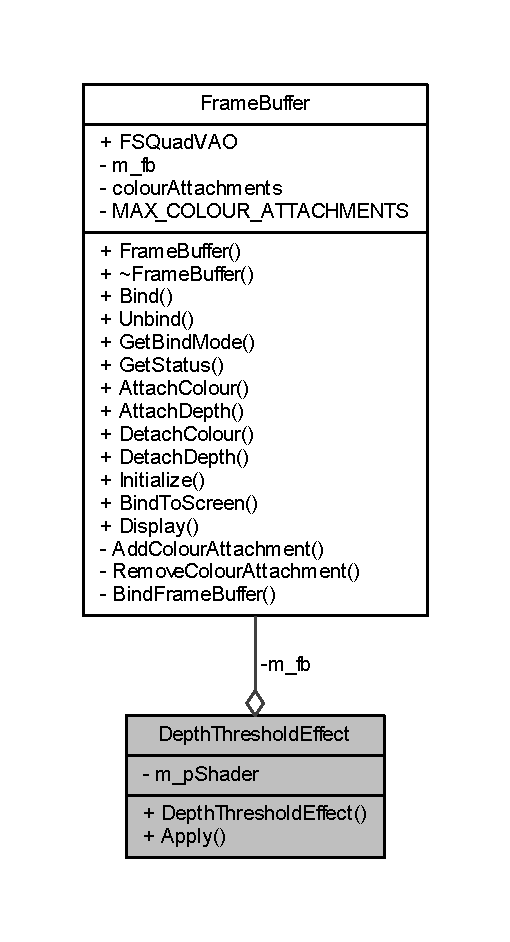
\includegraphics[width=245pt]{class_depth_threshold_effect__coll__graph}
\end{center}
\end{figure}
\subsection*{Public Member Functions}
\begin{DoxyCompactItemize}
\item 
\hyperlink{class_depth_threshold_effect_ae4e0bf5ce9847f019acb17000868803f}{Depth\+Threshold\+Effect} ()
\begin{DoxyCompactList}\small\item\em Initializes a new instance of the \hyperlink{class_depth_threshold_effect}{Depth\+Threshold\+Effect} class. \end{DoxyCompactList}\item 
void \hyperlink{class_depth_threshold_effect_ad7d1a9f0995d81f3f8ef607ffd75fc6a}{Apply} (G\+Luint input\+Tex, G\+Luint output\+Tex, float threshold)
\begin{DoxyCompactList}\small\item\em Applies the depth threshold effect. \end{DoxyCompactList}\end{DoxyCompactItemize}
\subsection*{Private Attributes}
\begin{DoxyCompactItemize}
\item 
\hyperlink{class_frame_buffer}{Frame\+Buffer} \hyperlink{class_depth_threshold_effect_a37003be12ef10a17d7b0d3e74b4290b1}{m\+\_\+fb}
\begin{DoxyCompactList}\small\item\em The frame buffer \end{DoxyCompactList}\item 
std\+::unique\+\_\+ptr$<$ \hyperlink{class_i_shader}{I\+Shader} $>$ const \& \hyperlink{class_depth_threshold_effect_a46e4bba75a147b68b493f4aef1981893}{m\+\_\+p\+Shader}
\begin{DoxyCompactList}\small\item\em The shader \end{DoxyCompactList}\end{DoxyCompactItemize}


\subsection{Detailed Description}


Definition at line 16 of file Depth\+Threshold\+Effect.\+h.



\subsection{Constructor \& Destructor Documentation}
\index{Depth\+Threshold\+Effect@{Depth\+Threshold\+Effect}!Depth\+Threshold\+Effect@{Depth\+Threshold\+Effect}}
\index{Depth\+Threshold\+Effect@{Depth\+Threshold\+Effect}!Depth\+Threshold\+Effect@{Depth\+Threshold\+Effect}}
\subsubsection[{\texorpdfstring{Depth\+Threshold\+Effect()}{DepthThresholdEffect()}}]{\setlength{\rightskip}{0pt plus 5cm}Depth\+Threshold\+Effect\+::\+Depth\+Threshold\+Effect (
\begin{DoxyParamCaption}
{}
\end{DoxyParamCaption}
)}\hypertarget{class_depth_threshold_effect_ae4e0bf5ce9847f019acb17000868803f}{}\label{class_depth_threshold_effect_ae4e0bf5ce9847f019acb17000868803f}


Initializes a new instance of the \hyperlink{class_depth_threshold_effect}{Depth\+Threshold\+Effect} class. 



Definition at line 5 of file Depth\+Threshold\+Effect.\+cpp.



References Depth\+Threshold\+Effect().



Referenced by Depth\+Threshold\+Effect(), and Render\+Manager\+A\+P\+I\+::\+Initialise().


\begin{DoxyCode}
6   : \hyperlink{class_depth_threshold_effect_a46e4bba75a147b68b493f4aef1981893}{m\_pShader}(\hyperlink{class_singleton_a74f32751d99bf3cc95fe17aba11f4b07}{ShaderLibrary::GetInstance}().GetShader(\textcolor{stringliteral}{"
      DepthThresholdEffect"}))
7 \{
8     
9 \}
\end{DoxyCode}


Here is the call graph for this function\+:\nopagebreak
\begin{figure}[H]
\begin{center}
\leavevmode
\includegraphics[width=195pt]{class_depth_threshold_effect_ae4e0bf5ce9847f019acb17000868803f_cgraph}
\end{center}
\end{figure}




Here is the caller graph for this function\+:
\nopagebreak
\begin{figure}[H]
\begin{center}
\leavevmode
\includegraphics[width=350pt]{class_depth_threshold_effect_ae4e0bf5ce9847f019acb17000868803f_icgraph}
\end{center}
\end{figure}




\subsection{Member Function Documentation}
\index{Depth\+Threshold\+Effect@{Depth\+Threshold\+Effect}!Apply@{Apply}}
\index{Apply@{Apply}!Depth\+Threshold\+Effect@{Depth\+Threshold\+Effect}}
\subsubsection[{\texorpdfstring{Apply(\+G\+Luint input\+Tex, G\+Luint output\+Tex, float threshold)}{Apply(GLuint inputTex, GLuint outputTex, float threshold)}}]{\setlength{\rightskip}{0pt plus 5cm}void Depth\+Threshold\+Effect\+::\+Apply (
\begin{DoxyParamCaption}
\item[{G\+Luint}]{input\+Tex, }
\item[{G\+Luint}]{output\+Tex, }
\item[{float}]{threshold}
\end{DoxyParamCaption}
)}\hypertarget{class_depth_threshold_effect_ad7d1a9f0995d81f3f8ef607ffd75fc6a}{}\label{class_depth_threshold_effect_ad7d1a9f0995d81f3f8ef607ffd75fc6a}


Applies the depth threshold effect. 


\begin{DoxyParams}{Parameters}
{\em input\+Tex} & The input tex.\\
\hline
{\em output\+Tex} & The output tex.\\
\hline
{\em threshold} & The threshold.\\
\hline
\end{DoxyParams}


Definition at line 11 of file Depth\+Threshold\+Effect.\+cpp.


\begin{DoxyCode}
12 \{
13     \hyperlink{class_depth_threshold_effect_a37003be12ef10a17d7b0d3e74b4290b1}{m\_fb}.\hyperlink{class_frame_buffer_ae7e61568475fba3b15e446c9061833ea}{Bind}();
14 
15     \hyperlink{class_depth_threshold_effect_a37003be12ef10a17d7b0d3e74b4290b1}{m\_fb}.\hyperlink{class_frame_buffer_a1556417c0dec00d1d24bdf0e84bc4c4d}{AttachColour}(0, outputTex);
16     glClear(GL\_COLOR\_BUFFER\_BIT | GL\_DEPTH\_BUFFER\_BIT);
17     \hyperlink{class_depth_threshold_effect_a46e4bba75a147b68b493f4aef1981893}{m\_pShader}->Bind();
18     \hyperlink{class_depth_threshold_effect_a46e4bba75a147b68b493f4aef1981893}{m\_pShader}->TransmitUniform(\textcolor{stringliteral}{"threshold"}, threshold);
19     glBindVertexArray(\hyperlink{class_frame_buffer_a22b0c9de2bef06e0de865684556a6677}{FrameBuffer::FSQuadVAO});
20     glActiveTexture(GL\_TEXTURE0 + 0);
21     glBindTexture(GL\_TEXTURE\_2D, inputTex);
22     \hyperlink{class_depth_threshold_effect_a46e4bba75a147b68b493f4aef1981893}{m\_pShader}->TransmitUniform(\textcolor{stringliteral}{"inputTex0"}, 0);
23     glDrawArrays(GL\_QUADS, 0, 4);
24     glBindVertexArray(NULL);
25 
26     \hyperlink{class_depth_threshold_effect_a37003be12ef10a17d7b0d3e74b4290b1}{m\_fb}.\hyperlink{class_frame_buffer_a1e114b325998ec4e4b9a9ea090d64ae8}{Unbind}();
27 \}
\end{DoxyCode}


\subsection{Member Data Documentation}
\index{Depth\+Threshold\+Effect@{Depth\+Threshold\+Effect}!m\+\_\+fb@{m\+\_\+fb}}
\index{m\+\_\+fb@{m\+\_\+fb}!Depth\+Threshold\+Effect@{Depth\+Threshold\+Effect}}
\subsubsection[{\texorpdfstring{m\+\_\+fb}{m_fb}}]{\setlength{\rightskip}{0pt plus 5cm}{\bf Frame\+Buffer} Depth\+Threshold\+Effect\+::m\+\_\+fb\hspace{0.3cm}{\ttfamily [private]}}\hypertarget{class_depth_threshold_effect_a37003be12ef10a17d7b0d3e74b4290b1}{}\label{class_depth_threshold_effect_a37003be12ef10a17d7b0d3e74b4290b1}


The frame buffer 



Definition at line 38 of file Depth\+Threshold\+Effect.\+h.

\index{Depth\+Threshold\+Effect@{Depth\+Threshold\+Effect}!m\+\_\+p\+Shader@{m\+\_\+p\+Shader}}
\index{m\+\_\+p\+Shader@{m\+\_\+p\+Shader}!Depth\+Threshold\+Effect@{Depth\+Threshold\+Effect}}
\subsubsection[{\texorpdfstring{m\+\_\+p\+Shader}{m_pShader}}]{\setlength{\rightskip}{0pt plus 5cm}std\+::unique\+\_\+ptr$<${\bf I\+Shader}$>$ const\& Depth\+Threshold\+Effect\+::m\+\_\+p\+Shader\hspace{0.3cm}{\ttfamily [private]}}\hypertarget{class_depth_threshold_effect_a46e4bba75a147b68b493f4aef1981893}{}\label{class_depth_threshold_effect_a46e4bba75a147b68b493f4aef1981893}


The shader 



Definition at line 43 of file Depth\+Threshold\+Effect.\+h.



The documentation for this class was generated from the following files\+:\begin{DoxyCompactItemize}
\item 
C\+:/\+Users/elizabeth/\+Documents/\+Git\+Hub/\+Engine/\+Open\+G\+L\+Engine/\+Open\+G\+L\+Engine/\hyperlink{_depth_threshold_effect_8h}{Depth\+Threshold\+Effect.\+h}\item 
C\+:/\+Users/elizabeth/\+Documents/\+Git\+Hub/\+Engine/\+Open\+G\+L\+Engine/\+Open\+G\+L\+Engine/\hyperlink{_depth_threshold_effect_8cpp}{Depth\+Threshold\+Effect.\+cpp}\end{DoxyCompactItemize}

\hypertarget{struct_directional_light}{}\section{Directional\+Light Struct Reference}
\label{struct_directional_light}\index{Directional\+Light@{Directional\+Light}}


{\ttfamily \#include $<$Light.\+h$>$}



Inheritance diagram for Directional\+Light\+:\nopagebreak
\begin{figure}[H]
\begin{center}
\leavevmode
\includegraphics[width=178pt]{struct_directional_light__inherit__graph}
\end{center}
\end{figure}


Collaboration diagram for Directional\+Light\+:\nopagebreak
\begin{figure}[H]
\begin{center}
\leavevmode
\includegraphics[width=178pt]{struct_directional_light__coll__graph}
\end{center}
\end{figure}
\subsection*{Public Member Functions}
\begin{DoxyCompactItemize}
\item 
\hyperlink{struct_directional_light_ac2b1a62d9ad6395b2f453b4544127bf1}{Directional\+Light} (\hyperlink{_types_8h_a3d0ce73e3199de81565fb01632415288}{vec3} const \&light\+Direction, \hyperlink{_types_8h_a3d0ce73e3199de81565fb01632415288}{vec3} const \&light\+Color=\hyperlink{_types_8h_a3d0ce73e3199de81565fb01632415288}{vec3}(1.\+0f, 1.\+0f, 1.\+0f), bool light\+Enabled=true)
\end{DoxyCompactItemize}
\subsection*{Public Attributes}
\begin{DoxyCompactItemize}
\item 
\hyperlink{_types_8h_a3d0ce73e3199de81565fb01632415288}{vec3} \hyperlink{struct_directional_light_a0fff081764e57e46c7342fc6c6849c1c}{color}
\item 
\hyperlink{_types_8h_a3d0ce73e3199de81565fb01632415288}{vec3} \hyperlink{struct_directional_light_a78a56aede026b50aa2606bf20c1b0871}{direction}
\end{DoxyCompactItemize}
\subsection*{Additional Inherited Members}


\subsection{Detailed Description}


Definition at line 49 of file Light.\+h.



\subsection{Constructor \& Destructor Documentation}
\index{Directional\+Light@{Directional\+Light}!Directional\+Light@{Directional\+Light}}
\index{Directional\+Light@{Directional\+Light}!Directional\+Light@{Directional\+Light}}
\subsubsection[{\texorpdfstring{Directional\+Light(vec3 const \&light\+Direction, vec3 const \&light\+Color=vec3(1.\+0f, 1.\+0f, 1.\+0f), bool light\+Enabled=true)}{DirectionalLight(vec3 const &lightDirection, vec3 const &lightColor=vec3(1.0f, 1.0f, 1.0f), bool lightEnabled=true)}}]{\setlength{\rightskip}{0pt plus 5cm}Directional\+Light\+::\+Directional\+Light (
\begin{DoxyParamCaption}
\item[{{\bf vec3} const \&}]{light\+Direction, }
\item[{{\bf vec3} const \&}]{light\+Color = {\ttfamily {\bf vec3}(1.0f,~1.0f,~1.0f)}, }
\item[{bool}]{light\+Enabled = {\ttfamily true}}
\end{DoxyParamCaption}
)\hspace{0.3cm}{\ttfamily [inline]}}\hypertarget{struct_directional_light_ac2b1a62d9ad6395b2f453b4544127bf1}{}\label{struct_directional_light_ac2b1a62d9ad6395b2f453b4544127bf1}


Definition at line 51 of file Light.\+h.



References direction, Directional\+Light(), Light\+::\+Light(), and L\+T\+\_\+\+Directional.



Referenced by Directional\+Light().


\begin{DoxyCode}
52     : \hyperlink{struct_light_a0df5e58af351bd13c996da2880be0dee}{Light}(\hyperlink{_light_8h_a3336214f41ddc8acd932fa9be957047da21fefd4273a9d89cb46b6610ade6ca01}{LT\_Directional}, lightEnabled)
53     , \hyperlink{struct_directional_light_a0fff081764e57e46c7342fc6c6849c1c}{color}(lightColor)
54     , \hyperlink{struct_directional_light_a78a56aede026b50aa2606bf20c1b0871}{direction}(lightDirection)
55   \{
56 
57   \}
\end{DoxyCode}


Here is the call graph for this function\+:\nopagebreak
\begin{figure}[H]
\begin{center}
\leavevmode
\includegraphics[width=316pt]{struct_directional_light_ac2b1a62d9ad6395b2f453b4544127bf1_cgraph}
\end{center}
\end{figure}




Here is the caller graph for this function\+:\nopagebreak
\begin{figure}[H]
\begin{center}
\leavevmode
\includegraphics[width=215pt]{struct_directional_light_ac2b1a62d9ad6395b2f453b4544127bf1_icgraph}
\end{center}
\end{figure}




\subsection{Member Data Documentation}
\index{Directional\+Light@{Directional\+Light}!color@{color}}
\index{color@{color}!Directional\+Light@{Directional\+Light}}
\subsubsection[{\texorpdfstring{color}{color}}]{\setlength{\rightskip}{0pt plus 5cm}{\bf vec3} Directional\+Light\+::color}\hypertarget{struct_directional_light_a0fff081764e57e46c7342fc6c6849c1c}{}\label{struct_directional_light_a0fff081764e57e46c7342fc6c6849c1c}


Definition at line 58 of file Light.\+h.

\index{Directional\+Light@{Directional\+Light}!direction@{direction}}
\index{direction@{direction}!Directional\+Light@{Directional\+Light}}
\subsubsection[{\texorpdfstring{direction}{direction}}]{\setlength{\rightskip}{0pt plus 5cm}{\bf vec3} Directional\+Light\+::direction}\hypertarget{struct_directional_light_a78a56aede026b50aa2606bf20c1b0871}{}\label{struct_directional_light_a78a56aede026b50aa2606bf20c1b0871}


Definition at line 59 of file Light.\+h.



Referenced by Directional\+Light().



The documentation for this struct was generated from the following file\+:\begin{DoxyCompactItemize}
\item 
C\+:/\+Users/elizabeth/\+Documents/\+Git\+Hub/\+Engine/\+Open\+G\+L\+Engine/\+Open\+G\+L\+Engine/\hyperlink{_light_8h}{Light.\+h}\end{DoxyCompactItemize}

\hypertarget{class_directional_lighting_effect}{}\section{Directional\+Lighting\+Effect Class Reference}
\label{class_directional_lighting_effect}\index{Directional\+Lighting\+Effect@{Directional\+Lighting\+Effect}}


{\ttfamily \#include $<$Directional\+Lighting\+Effect.\+h$>$}



Collaboration diagram for Directional\+Lighting\+Effect\+:\nopagebreak
\begin{figure}[H]
\begin{center}
\leavevmode
\includegraphics[width=245pt]{class_directional_lighting_effect__coll__graph}
\end{center}
\end{figure}
\subsection*{Public Member Functions}
\begin{DoxyCompactItemize}
\item 
\hyperlink{class_directional_lighting_effect_a4ee635d9d9ed5ce5ebb5cef463e67723}{Directional\+Lighting\+Effect} ()
\begin{DoxyCompactList}\small\item\em Initializes a new instance of the \hyperlink{class_directional_lighting_effect}{Directional\+Lighting\+Effect} class. \end{DoxyCompactList}\item 
void \hyperlink{class_directional_lighting_effect_a8cca766638f16ac83b4339e5855e0a8f}{Apply} (G\+Luint normal\+Tex, G\+Luint output\+Tex, \hyperlink{_types_8h_a3d0ce73e3199de81565fb01632415288}{vec3} colour, \hyperlink{_types_8h_a3d0ce73e3199de81565fb01632415288}{vec3} direction)
\begin{DoxyCompactList}\small\item\em Applies the directional lighting effect. \end{DoxyCompactList}\end{DoxyCompactItemize}
\subsection*{Private Attributes}
\begin{DoxyCompactItemize}
\item 
\hyperlink{class_frame_buffer}{Frame\+Buffer} \hyperlink{class_directional_lighting_effect_a7e94bd539e7cb254d32bdffa4d8aae57}{m\+\_\+fb}
\begin{DoxyCompactList}\small\item\em The frame buffer \end{DoxyCompactList}\item 
std\+::unique\+\_\+ptr$<$ \hyperlink{class_i_shader}{I\+Shader} $>$ const \& \hyperlink{class_directional_lighting_effect_ad53c001d1de64b1b539b68d5de943c4f}{m\+\_\+p\+Shader}
\begin{DoxyCompactList}\small\item\em The shader \end{DoxyCompactList}\end{DoxyCompactItemize}


\subsection{Detailed Description}


Definition at line 15 of file Directional\+Lighting\+Effect.\+h.



\subsection{Constructor \& Destructor Documentation}
\index{Directional\+Lighting\+Effect@{Directional\+Lighting\+Effect}!Directional\+Lighting\+Effect@{Directional\+Lighting\+Effect}}
\index{Directional\+Lighting\+Effect@{Directional\+Lighting\+Effect}!Directional\+Lighting\+Effect@{Directional\+Lighting\+Effect}}
\subsubsection[{\texorpdfstring{Directional\+Lighting\+Effect()}{DirectionalLightingEffect()}}]{\setlength{\rightskip}{0pt plus 5cm}Directional\+Lighting\+Effect\+::\+Directional\+Lighting\+Effect (
\begin{DoxyParamCaption}
{}
\end{DoxyParamCaption}
)}\hypertarget{class_directional_lighting_effect_a4ee635d9d9ed5ce5ebb5cef463e67723}{}\label{class_directional_lighting_effect_a4ee635d9d9ed5ce5ebb5cef463e67723}


Initializes a new instance of the \hyperlink{class_directional_lighting_effect}{Directional\+Lighting\+Effect} class. 



Definition at line 5 of file Directional\+Lighting\+Effect.\+cpp.



References Directional\+Lighting\+Effect().



Referenced by Directional\+Lighting\+Effect(), and Render\+Manager\+A\+P\+I\+::\+Initialise().


\begin{DoxyCode}
6   : \hyperlink{class_directional_lighting_effect_ad53c001d1de64b1b539b68d5de943c4f}{m\_pShader}(\hyperlink{class_singleton_a74f32751d99bf3cc95fe17aba11f4b07}{ShaderLibrary::GetInstance}().GetShader(\textcolor{stringliteral}{"
      DirectionalLightingEffect"}))
7 \{
8 
9 \}
\end{DoxyCode}


Here is the call graph for this function\+:\nopagebreak
\begin{figure}[H]
\begin{center}
\leavevmode
\includegraphics[width=207pt]{class_directional_lighting_effect_a4ee635d9d9ed5ce5ebb5cef463e67723_cgraph}
\end{center}
\end{figure}




Here is the caller graph for this function\+:
\nopagebreak
\begin{figure}[H]
\begin{center}
\leavevmode
\includegraphics[width=350pt]{class_directional_lighting_effect_a4ee635d9d9ed5ce5ebb5cef463e67723_icgraph}
\end{center}
\end{figure}




\subsection{Member Function Documentation}
\index{Directional\+Lighting\+Effect@{Directional\+Lighting\+Effect}!Apply@{Apply}}
\index{Apply@{Apply}!Directional\+Lighting\+Effect@{Directional\+Lighting\+Effect}}
\subsubsection[{\texorpdfstring{Apply(\+G\+Luint normal\+Tex, G\+Luint output\+Tex, vec3 colour, vec3 direction)}{Apply(GLuint normalTex, GLuint outputTex, vec3 colour, vec3 direction)}}]{\setlength{\rightskip}{0pt plus 5cm}void Directional\+Lighting\+Effect\+::\+Apply (
\begin{DoxyParamCaption}
\item[{G\+Luint}]{normal\+Tex, }
\item[{G\+Luint}]{output\+Tex, }
\item[{{\bf vec3}}]{colour, }
\item[{{\bf vec3}}]{direction}
\end{DoxyParamCaption}
)}\hypertarget{class_directional_lighting_effect_a8cca766638f16ac83b4339e5855e0a8f}{}\label{class_directional_lighting_effect_a8cca766638f16ac83b4339e5855e0a8f}


Applies the directional lighting effect. 


\begin{DoxyParams}{Parameters}
{\em normal\+Tex} & The normal tex.\\
\hline
{\em output\+Tex} & The output tex.\\
\hline
{\em colour} & The colour.\\
\hline
{\em direction} & The direction.\\
\hline
\end{DoxyParams}


Definition at line 11 of file Directional\+Lighting\+Effect.\+cpp.


\begin{DoxyCode}
12 \{
13   \hyperlink{class_directional_lighting_effect_a7e94bd539e7cb254d32bdffa4d8aae57}{m\_fb}.\hyperlink{class_frame_buffer_ae7e61568475fba3b15e446c9061833ea}{Bind}();
14 
15   \hyperlink{class_directional_lighting_effect_a7e94bd539e7cb254d32bdffa4d8aae57}{m\_fb}.\hyperlink{class_frame_buffer_a1556417c0dec00d1d24bdf0e84bc4c4d}{AttachColour}(0, outputTex);
16   glClear(GL\_COLOR\_BUFFER\_BIT | GL\_DEPTH\_BUFFER\_BIT);
17   \hyperlink{class_directional_lighting_effect_ad53c001d1de64b1b539b68d5de943c4f}{m\_pShader}->Bind();
18   \hyperlink{class_directional_lighting_effect_ad53c001d1de64b1b539b68d5de943c4f}{m\_pShader}->TransmitUniform(\textcolor{stringliteral}{"LIGHT\_COLOUR"}, colour);
19   \hyperlink{class_directional_lighting_effect_ad53c001d1de64b1b539b68d5de943c4f}{m\_pShader}->TransmitUniform(\textcolor{stringliteral}{"LIGHT\_DIRECTION"}, direction);
20   glBindVertexArray(\hyperlink{class_frame_buffer_a22b0c9de2bef06e0de865684556a6677}{FrameBuffer::FSQuadVAO});
21   glActiveTexture(GL\_TEXTURE0 + 0);
22   glBindTexture(GL\_TEXTURE\_2D, normalTex);
23   \hyperlink{class_directional_lighting_effect_ad53c001d1de64b1b539b68d5de943c4f}{m\_pShader}->TransmitUniform(\textcolor{stringliteral}{"inputTex0"}, 0);
24   glDrawArrays(GL\_QUADS, 0, 4);
25   glBindVertexArray(NULL);
26 
27   \hyperlink{class_directional_lighting_effect_a7e94bd539e7cb254d32bdffa4d8aae57}{m\_fb}.\hyperlink{class_frame_buffer_a1e114b325998ec4e4b9a9ea090d64ae8}{Unbind}();
28 \}
\end{DoxyCode}


\subsection{Member Data Documentation}
\index{Directional\+Lighting\+Effect@{Directional\+Lighting\+Effect}!m\+\_\+fb@{m\+\_\+fb}}
\index{m\+\_\+fb@{m\+\_\+fb}!Directional\+Lighting\+Effect@{Directional\+Lighting\+Effect}}
\subsubsection[{\texorpdfstring{m\+\_\+fb}{m_fb}}]{\setlength{\rightskip}{0pt plus 5cm}{\bf Frame\+Buffer} Directional\+Lighting\+Effect\+::m\+\_\+fb\hspace{0.3cm}{\ttfamily [private]}}\hypertarget{class_directional_lighting_effect_a7e94bd539e7cb254d32bdffa4d8aae57}{}\label{class_directional_lighting_effect_a7e94bd539e7cb254d32bdffa4d8aae57}


The frame buffer 



Definition at line 38 of file Directional\+Lighting\+Effect.\+h.

\index{Directional\+Lighting\+Effect@{Directional\+Lighting\+Effect}!m\+\_\+p\+Shader@{m\+\_\+p\+Shader}}
\index{m\+\_\+p\+Shader@{m\+\_\+p\+Shader}!Directional\+Lighting\+Effect@{Directional\+Lighting\+Effect}}
\subsubsection[{\texorpdfstring{m\+\_\+p\+Shader}{m_pShader}}]{\setlength{\rightskip}{0pt plus 5cm}std\+::unique\+\_\+ptr$<${\bf I\+Shader}$>$ const\& Directional\+Lighting\+Effect\+::m\+\_\+p\+Shader\hspace{0.3cm}{\ttfamily [private]}}\hypertarget{class_directional_lighting_effect_ad53c001d1de64b1b539b68d5de943c4f}{}\label{class_directional_lighting_effect_ad53c001d1de64b1b539b68d5de943c4f}


The shader 



Definition at line 43 of file Directional\+Lighting\+Effect.\+h.



The documentation for this class was generated from the following files\+:\begin{DoxyCompactItemize}
\item 
C\+:/\+Users/elizabeth/\+Documents/\+Git\+Hub/\+Engine/\+Open\+G\+L\+Engine/\+Open\+G\+L\+Engine/\hyperlink{_directional_lighting_effect_8h}{Directional\+Lighting\+Effect.\+h}\item 
C\+:/\+Users/elizabeth/\+Documents/\+Git\+Hub/\+Engine/\+Open\+G\+L\+Engine/\+Open\+G\+L\+Engine/\hyperlink{_directional_lighting_effect_8cpp}{Directional\+Lighting\+Effect.\+cpp}\end{DoxyCompactItemize}

\hypertarget{class_d_x_engine}{}\section{D\+X\+Engine Class Reference}
\label{class_d_x_engine}\index{D\+X\+Engine@{D\+X\+Engine}}


{\ttfamily \#include $<$D\+X\+Engine.\+h$>$}



Inheritance diagram for D\+X\+Engine\+:\nopagebreak
\begin{figure}[H]
\begin{center}
\leavevmode
\includegraphics[width=217pt]{class_d_x_engine__inherit__graph}
\end{center}
\end{figure}


Collaboration diagram for D\+X\+Engine\+:\nopagebreak
\begin{figure}[H]
\begin{center}
\leavevmode
\includegraphics[width=217pt]{class_d_x_engine__coll__graph}
\end{center}
\end{figure}
\subsection*{Public Member Functions}
\begin{DoxyCompactItemize}
\item 
virtual void \hyperlink{class_d_x_engine_a8b5413a8d83f7a1a88b0dcb1e9ab378c}{Initialise} (int screen\+Width, int screen\+Height) override
\begin{DoxyCompactList}\small\item\em Initialises the engine. \end{DoxyCompactList}\item 
virtual void \hyperlink{class_d_x_engine_a11d8bf69f1673ef1715b7ffc899190e1}{Begin\+Render} () override
\begin{DoxyCompactList}\small\item\em Begins the render. \end{DoxyCompactList}\item 
virtual void \hyperlink{class_d_x_engine_a1326b18c1e4cc8e74f8337e13e0bfac0}{End\+Render} () override
\begin{DoxyCompactList}\small\item\em Ends the render. \end{DoxyCompactList}\item 
virtual bool \hyperlink{class_d_x_engine_a6dadbd253449bee8787178e47676d1f5}{Begin\+Update} () override
\begin{DoxyCompactList}\small\item\em Begins the update. \end{DoxyCompactList}\item 
virtual void \hyperlink{class_d_x_engine_a7c6c49cdd2b24a81c19ee2d52cb1045b}{End\+Update} () override
\begin{DoxyCompactList}\small\item\em Ends the update. \end{DoxyCompactList}\item 
virtual \hyperlink{class_i_shader}{I\+Shader} $\ast$ \hyperlink{class_d_x_engine_ac3f1b18e87c40707b091a7ef42656729}{Create\+Shader} (\hyperlink{_types_8h_ad453f9f71ce1f9153fb748d6bb25e454}{string} const \&name, \hyperlink{_types_8h_ad453f9f71ce1f9153fb748d6bb25e454}{string} const \&vert\+File\+Path, \hyperlink{_types_8h_ad453f9f71ce1f9153fb748d6bb25e454}{string} const \&frag\+File\+Path, std\+::vector$<$ \hyperlink{_types_8h_ad453f9f71ce1f9153fb748d6bb25e454}{string} $>$ const \&attributes, std\+::vector$<$ \hyperlink{_types_8h_ad453f9f71ce1f9153fb748d6bb25e454}{string} $>$ const \&uniforms) const  override
\begin{DoxyCompactList}\small\item\em Creates the shader. \end{DoxyCompactList}\item 
virtual \hyperlink{class_i_renderable_object}{I\+Renderable\+Object} $\ast$ \hyperlink{class_d_x_engine_ab640a4514292c84b528ee0f197c7deda}{Create\+Renderable\+Object} (\hyperlink{_types_8h_ad453f9f71ce1f9153fb748d6bb25e454}{string} const \&name, \hyperlink{_types_8h_ad453f9f71ce1f9153fb748d6bb25e454}{string} const \&filename) const  override
\begin{DoxyCompactList}\small\item\em Creates the renderable object. \end{DoxyCompactList}\item 
virtual \hyperlink{class_i_input_handler}{I\+Input\+Handler} $\ast$ \hyperlink{class_d_x_engine_ab7158b320580a4df4cf7feebb06f9a6f}{Create\+Input\+Handler} () override
\begin{DoxyCompactList}\small\item\em Creates the input handler. \end{DoxyCompactList}\end{DoxyCompactItemize}
\subsection*{Static Public Member Functions}
\begin{DoxyCompactItemize}
\item 
static \hyperlink{class_i_engine}{I\+Engine} $\ast$ \hyperlink{class_d_x_engine_acdb42db6ccec8c1dfcd7cd24d24202cb}{Create} ()
\begin{DoxyCompactList}\small\item\em Creates this instance. \end{DoxyCompactList}\end{DoxyCompactItemize}
\subsection*{Private Member Functions}
\begin{DoxyCompactItemize}
\item 
\hyperlink{class_d_x_engine_a081ec6a228228bfcc35c127a27c09ad0}{D\+X\+Engine} ()
\begin{DoxyCompactList}\small\item\em Prevents a default instance of the \hyperlink{class_d_x_engine}{D\+X\+Engine} class from being created. \end{DoxyCompactList}\item 
virtual \hyperlink{class_d_x_engine_a8498629b33c7c49ead2b0f62779c7bd8}{$\sim$\+D\+X\+Engine} () override
\begin{DoxyCompactList}\small\item\em Finalizes an instance of the \hyperlink{class_d_x_engine}{D\+X\+Engine} class. \end{DoxyCompactList}\end{DoxyCompactItemize}


\subsection{Detailed Description}


Definition at line 15 of file D\+X\+Engine.\+h.



\subsection{Constructor \& Destructor Documentation}
\index{D\+X\+Engine@{D\+X\+Engine}!D\+X\+Engine@{D\+X\+Engine}}
\index{D\+X\+Engine@{D\+X\+Engine}!D\+X\+Engine@{D\+X\+Engine}}
\subsubsection[{\texorpdfstring{D\+X\+Engine()}{DXEngine()}}]{\setlength{\rightskip}{0pt plus 5cm}D\+X\+Engine\+::\+D\+X\+Engine (
\begin{DoxyParamCaption}
{}
\end{DoxyParamCaption}
)\hspace{0.3cm}{\ttfamily [private]}}\hypertarget{class_d_x_engine_a081ec6a228228bfcc35c127a27c09ad0}{}\label{class_d_x_engine_a081ec6a228228bfcc35c127a27c09ad0}


Prevents a default instance of the \hyperlink{class_d_x_engine}{D\+X\+Engine} class from being created. 



Definition at line 48 of file D\+X\+Engine.\+cpp.



Referenced by Create().


\begin{DoxyCode}
49 \{
50 
51 \}
\end{DoxyCode}


Here is the caller graph for this function\+:\nopagebreak
\begin{figure}[H]
\begin{center}
\leavevmode
\includegraphics[width=316pt]{class_d_x_engine_a081ec6a228228bfcc35c127a27c09ad0_icgraph}
\end{center}
\end{figure}


\index{D\+X\+Engine@{D\+X\+Engine}!````~D\+X\+Engine@{$\sim$\+D\+X\+Engine}}
\index{````~D\+X\+Engine@{$\sim$\+D\+X\+Engine}!D\+X\+Engine@{D\+X\+Engine}}
\subsubsection[{\texorpdfstring{$\sim$\+D\+X\+Engine() override}{~DXEngine() override}}]{\setlength{\rightskip}{0pt plus 5cm}D\+X\+Engine\+::$\sim$\+D\+X\+Engine (
\begin{DoxyParamCaption}
{}
\end{DoxyParamCaption}
)\hspace{0.3cm}{\ttfamily [override]}, {\ttfamily [private]}, {\ttfamily [virtual]}}\hypertarget{class_d_x_engine_a8498629b33c7c49ead2b0f62779c7bd8}{}\label{class_d_x_engine_a8498629b33c7c49ead2b0f62779c7bd8}


Finalizes an instance of the \hyperlink{class_d_x_engine}{D\+X\+Engine} class. 



Definition at line 53 of file D\+X\+Engine.\+cpp.


\begin{DoxyCode}
54 \{
55 
56 \}
\end{DoxyCode}


\subsection{Member Function Documentation}
\index{D\+X\+Engine@{D\+X\+Engine}!Begin\+Render@{Begin\+Render}}
\index{Begin\+Render@{Begin\+Render}!D\+X\+Engine@{D\+X\+Engine}}
\subsubsection[{\texorpdfstring{Begin\+Render() override}{BeginRender() override}}]{\setlength{\rightskip}{0pt plus 5cm}void D\+X\+Engine\+::\+Begin\+Render (
\begin{DoxyParamCaption}
{}
\end{DoxyParamCaption}
)\hspace{0.3cm}{\ttfamily [override]}, {\ttfamily [virtual]}}\hypertarget{class_d_x_engine_a11d8bf69f1673ef1715b7ffc899190e1}{}\label{class_d_x_engine_a11d8bf69f1673ef1715b7ffc899190e1}


Begins the render. 



Implements \hyperlink{class_i_engine_ac07a33654b17337655bb1e36f28991bb}{I\+Engine}.



Definition at line 13 of file D\+X\+Engine.\+cpp.


\begin{DoxyCode}
14 \{
15   \textcolor{keywordflow}{throw} std::logic\_error(\textcolor{stringliteral}{"The method or operation is not implemented."});
16 \}
\end{DoxyCode}
\index{D\+X\+Engine@{D\+X\+Engine}!Begin\+Update@{Begin\+Update}}
\index{Begin\+Update@{Begin\+Update}!D\+X\+Engine@{D\+X\+Engine}}
\subsubsection[{\texorpdfstring{Begin\+Update() override}{BeginUpdate() override}}]{\setlength{\rightskip}{0pt plus 5cm}bool D\+X\+Engine\+::\+Begin\+Update (
\begin{DoxyParamCaption}
{}
\end{DoxyParamCaption}
)\hspace{0.3cm}{\ttfamily [override]}, {\ttfamily [virtual]}}\hypertarget{class_d_x_engine_a6dadbd253449bee8787178e47676d1f5}{}\label{class_d_x_engine_a6dadbd253449bee8787178e47676d1f5}


Begins the update. 

\begin{DoxyReturn}{Returns}

\end{DoxyReturn}


Implements \hyperlink{class_i_engine_a5da41643af01472fe1b4aa0ac84fb447}{I\+Engine}.



Definition at line 23 of file D\+X\+Engine.\+cpp.


\begin{DoxyCode}
24 \{
25   \textcolor{keywordflow}{throw} std::logic\_error(\textcolor{stringliteral}{"The method or operation is not implemented."});
26 \}
\end{DoxyCode}
\index{D\+X\+Engine@{D\+X\+Engine}!Create@{Create}}
\index{Create@{Create}!D\+X\+Engine@{D\+X\+Engine}}
\subsubsection[{\texorpdfstring{Create()}{Create()}}]{\setlength{\rightskip}{0pt plus 5cm}{\bf I\+Engine} $\ast$ D\+X\+Engine\+::\+Create (
\begin{DoxyParamCaption}
{}
\end{DoxyParamCaption}
)\hspace{0.3cm}{\ttfamily [static]}}\hypertarget{class_d_x_engine_acdb42db6ccec8c1dfcd7cd24d24202cb}{}\label{class_d_x_engine_acdb42db6ccec8c1dfcd7cd24d24202cb}


Creates this instance. 

\begin{DoxyReturn}{Returns}
I\+Engine$\ast$
\end{DoxyReturn}


Definition at line 3 of file D\+X\+Engine.\+cpp.



References D\+X\+Engine().


\begin{DoxyCode}
4 \{
5   \textcolor{keywordflow}{return} \textcolor{keyword}{new} \hyperlink{class_d_x_engine_a081ec6a228228bfcc35c127a27c09ad0}{DXEngine}();
6 \}
\end{DoxyCode}


Here is the call graph for this function\+:\nopagebreak
\begin{figure}[H]
\begin{center}
\leavevmode
\includegraphics[width=316pt]{class_d_x_engine_acdb42db6ccec8c1dfcd7cd24d24202cb_cgraph}
\end{center}
\end{figure}


\index{D\+X\+Engine@{D\+X\+Engine}!Create\+Input\+Handler@{Create\+Input\+Handler}}
\index{Create\+Input\+Handler@{Create\+Input\+Handler}!D\+X\+Engine@{D\+X\+Engine}}
\subsubsection[{\texorpdfstring{Create\+Input\+Handler() override}{CreateInputHandler() override}}]{\setlength{\rightskip}{0pt plus 5cm}{\bf I\+Input\+Handler} $\ast$ D\+X\+Engine\+::\+Create\+Input\+Handler (
\begin{DoxyParamCaption}
{}
\end{DoxyParamCaption}
)\hspace{0.3cm}{\ttfamily [override]}, {\ttfamily [virtual]}}\hypertarget{class_d_x_engine_ab7158b320580a4df4cf7feebb06f9a6f}{}\label{class_d_x_engine_ab7158b320580a4df4cf7feebb06f9a6f}


Creates the input handler. 

\begin{DoxyReturn}{Returns}

\end{DoxyReturn}


Implements \hyperlink{class_i_engine_a4b4ccaa2ff5d54ac695697f14c4f4b47}{I\+Engine}.



Definition at line 43 of file D\+X\+Engine.\+cpp.


\begin{DoxyCode}
44 \{
45   \textcolor{keywordflow}{throw} std::logic\_error(\textcolor{stringliteral}{"The method or operation is not implemented."});
46 \}
\end{DoxyCode}
\index{D\+X\+Engine@{D\+X\+Engine}!Create\+Renderable\+Object@{Create\+Renderable\+Object}}
\index{Create\+Renderable\+Object@{Create\+Renderable\+Object}!D\+X\+Engine@{D\+X\+Engine}}
\subsubsection[{\texorpdfstring{Create\+Renderable\+Object(string const \&name, string const \&filename) const  override}{CreateRenderableObject(string const &name, string const &filename) const  override}}]{\setlength{\rightskip}{0pt plus 5cm}{\bf I\+Renderable\+Object} $\ast$ D\+X\+Engine\+::\+Create\+Renderable\+Object (
\begin{DoxyParamCaption}
\item[{{\bf string} const \&}]{name, }
\item[{{\bf string} const \&}]{filename}
\end{DoxyParamCaption}
) const\hspace{0.3cm}{\ttfamily [override]}, {\ttfamily [virtual]}}\hypertarget{class_d_x_engine_ab640a4514292c84b528ee0f197c7deda}{}\label{class_d_x_engine_ab640a4514292c84b528ee0f197c7deda}


Creates the renderable object. 


\begin{DoxyParams}{Parameters}
{\em name} & The name.\\
\hline
{\em filename} & The filename.\\
\hline
\end{DoxyParams}
\begin{DoxyReturn}{Returns}

\end{DoxyReturn}


Implements \hyperlink{class_i_engine_a263c5f4b936dbb4f2ec08df3c0b5b49e}{I\+Engine}.



Definition at line 38 of file D\+X\+Engine.\+cpp.


\begin{DoxyCode}
39 \{
40   \textcolor{keywordflow}{throw} std::logic\_error(\textcolor{stringliteral}{"The method or operation is not implemented."});
41 \}
\end{DoxyCode}
\index{D\+X\+Engine@{D\+X\+Engine}!Create\+Shader@{Create\+Shader}}
\index{Create\+Shader@{Create\+Shader}!D\+X\+Engine@{D\+X\+Engine}}
\subsubsection[{\texorpdfstring{Create\+Shader(string const \&name, string const \&vert\+File\+Path, string const \&frag\+File\+Path, std\+::vector$<$ string $>$ const \&attributes, std\+::vector$<$ string $>$ const \&uniforms) const  override}{CreateShader(string const &name, string const &vertFilePath, string const &fragFilePath, std::vector< string > const &attributes, std::vector< string > const &uniforms) const  override}}]{\setlength{\rightskip}{0pt plus 5cm}{\bf I\+Shader} $\ast$ D\+X\+Engine\+::\+Create\+Shader (
\begin{DoxyParamCaption}
\item[{{\bf string} const \&}]{name, }
\item[{{\bf string} const \&}]{vert\+File\+Path, }
\item[{{\bf string} const \&}]{frag\+File\+Path, }
\item[{std\+::vector$<$ {\bf string} $>$ const \&}]{attributes, }
\item[{std\+::vector$<$ {\bf string} $>$ const \&}]{uniforms}
\end{DoxyParamCaption}
) const\hspace{0.3cm}{\ttfamily [override]}, {\ttfamily [virtual]}}\hypertarget{class_d_x_engine_ac3f1b18e87c40707b091a7ef42656729}{}\label{class_d_x_engine_ac3f1b18e87c40707b091a7ef42656729}


Creates the shader. 


\begin{DoxyParams}{Parameters}
{\em name} & The name.\\
\hline
{\em vert\+File\+Path} & The vert file path.\\
\hline
{\em frag\+File\+Path} & The frag file path.\\
\hline
{\em attributes} & The attributes.\\
\hline
{\em uniforms} & The uniforms.\\
\hline
\end{DoxyParams}
\begin{DoxyReturn}{Returns}

\end{DoxyReturn}


Implements \hyperlink{class_i_engine_aa42fdef0b3b3741e4a4de1821aaa8cd6}{I\+Engine}.



Definition at line 33 of file D\+X\+Engine.\+cpp.


\begin{DoxyCode}
34 \{
35   \textcolor{keywordflow}{throw} std::logic\_error(\textcolor{stringliteral}{"The method or operation is not implemented."});
36 \}
\end{DoxyCode}
\index{D\+X\+Engine@{D\+X\+Engine}!End\+Render@{End\+Render}}
\index{End\+Render@{End\+Render}!D\+X\+Engine@{D\+X\+Engine}}
\subsubsection[{\texorpdfstring{End\+Render() override}{EndRender() override}}]{\setlength{\rightskip}{0pt plus 5cm}void D\+X\+Engine\+::\+End\+Render (
\begin{DoxyParamCaption}
{}
\end{DoxyParamCaption}
)\hspace{0.3cm}{\ttfamily [override]}, {\ttfamily [virtual]}}\hypertarget{class_d_x_engine_a1326b18c1e4cc8e74f8337e13e0bfac0}{}\label{class_d_x_engine_a1326b18c1e4cc8e74f8337e13e0bfac0}


Ends the render. 



Implements \hyperlink{class_i_engine_a07693c65faccf9ae4d75ef6f916e6e25}{I\+Engine}.



Definition at line 18 of file D\+X\+Engine.\+cpp.


\begin{DoxyCode}
19 \{
20   \textcolor{keywordflow}{throw} std::logic\_error(\textcolor{stringliteral}{"The method or operation is not implemented."});
21 \}
\end{DoxyCode}
\index{D\+X\+Engine@{D\+X\+Engine}!End\+Update@{End\+Update}}
\index{End\+Update@{End\+Update}!D\+X\+Engine@{D\+X\+Engine}}
\subsubsection[{\texorpdfstring{End\+Update() override}{EndUpdate() override}}]{\setlength{\rightskip}{0pt plus 5cm}void D\+X\+Engine\+::\+End\+Update (
\begin{DoxyParamCaption}
{}
\end{DoxyParamCaption}
)\hspace{0.3cm}{\ttfamily [override]}, {\ttfamily [virtual]}}\hypertarget{class_d_x_engine_a7c6c49cdd2b24a81c19ee2d52cb1045b}{}\label{class_d_x_engine_a7c6c49cdd2b24a81c19ee2d52cb1045b}


Ends the update. 



Implements \hyperlink{class_i_engine_afbacb27cbd19a8d63dbd6c40e4f089f9}{I\+Engine}.



Definition at line 28 of file D\+X\+Engine.\+cpp.


\begin{DoxyCode}
29 \{
30   \textcolor{keywordflow}{throw} std::logic\_error(\textcolor{stringliteral}{"The method or operation is not implemented."});
31 \}
\end{DoxyCode}
\index{D\+X\+Engine@{D\+X\+Engine}!Initialise@{Initialise}}
\index{Initialise@{Initialise}!D\+X\+Engine@{D\+X\+Engine}}
\subsubsection[{\texorpdfstring{Initialise(int screen\+Width, int screen\+Height) override}{Initialise(int screenWidth, int screenHeight) override}}]{\setlength{\rightskip}{0pt plus 5cm}void D\+X\+Engine\+::\+Initialise (
\begin{DoxyParamCaption}
\item[{int}]{screen\+Width, }
\item[{int}]{screen\+Height}
\end{DoxyParamCaption}
)\hspace{0.3cm}{\ttfamily [override]}, {\ttfamily [virtual]}}\hypertarget{class_d_x_engine_a8b5413a8d83f7a1a88b0dcb1e9ab378c}{}\label{class_d_x_engine_a8b5413a8d83f7a1a88b0dcb1e9ab378c}


Initialises the engine. 


\begin{DoxyParams}{Parameters}
{\em screen\+Width} & Width of the screen.\\
\hline
{\em screen\+Height} & Height of the screen.\\
\hline
\end{DoxyParams}


Implements \hyperlink{class_i_engine_a2033b147f3b325d0194b746048a6200e}{I\+Engine}.



Definition at line 8 of file D\+X\+Engine.\+cpp.


\begin{DoxyCode}
9 \{
10   \textcolor{keywordflow}{throw} std::logic\_error(\textcolor{stringliteral}{"The method or operation is not implemented."});
11 \}
\end{DoxyCode}


The documentation for this class was generated from the following files\+:\begin{DoxyCompactItemize}
\item 
C\+:/\+Users/elizabeth/\+Documents/\+Git\+Hub/\+Engine/\+Open\+G\+L\+Engine/\+Open\+G\+L\+Engine/\hyperlink{_d_x_engine_8h}{D\+X\+Engine.\+h}\item 
C\+:/\+Users/elizabeth/\+Documents/\+Git\+Hub/\+Engine/\+Open\+G\+L\+Engine/\+Open\+G\+L\+Engine/\hyperlink{_d_x_engine_8cpp}{D\+X\+Engine.\+cpp}\end{DoxyCompactItemize}

\hypertarget{class_engine_a_p_i}{}\section{Engine\+A\+PI Class Reference}
\label{class_engine_a_p_i}\index{Engine\+A\+PI@{Engine\+A\+PI}}


{\ttfamily \#include $<$Engine\+A\+P\+I.\+h$>$}



Collaboration diagram for Engine\+A\+PI\+:\nopagebreak
\begin{figure}[H]
\begin{center}
\leavevmode
\includegraphics[width=157pt]{class_engine_a_p_i__coll__graph}
\end{center}
\end{figure}
\subsection*{Static Public Member Functions}
\begin{DoxyCompactItemize}
\item 
static void \hyperlink{class_engine_a_p_i_a86c6e645c223e40e553f037217acb83d}{Create} (int api)
\begin{DoxyCompactList}\small\item\em Exposes the functions in the A\+PI. \end{DoxyCompactList}\item 
static void \hyperlink{class_engine_a_p_i_a3913e2d46563231d499ef12b0079e622}{Expose} (\hyperlink{_lua_context_8h_a2ffcc2d3ed21165072a1d7b61259bf14}{Lua\+Context\+Handle} context\+Handle, \hyperlink{_types_8h_ad453f9f71ce1f9153fb748d6bb25e454}{string} lua\+A\+P\+I\+Name)
\begin{DoxyCompactList}\small\item\em Exposes the specified functions. \end{DoxyCompactList}\item 
static \hyperlink{class_i_engine}{I\+Engine} $\ast$ \hyperlink{class_engine_a_p_i_a6cecc94147f6fed1c2f886c082051bc7}{Get\+Engine} ()
\begin{DoxyCompactList}\small\item\em Gets the engine. \end{DoxyCompactList}\end{DoxyCompactItemize}
\subsection*{Static Private Attributes}
\begin{DoxyCompactItemize}
\item 
static std\+::unique\+\_\+ptr$<$ \hyperlink{class_i_engine}{I\+Engine} $>$ \hyperlink{class_engine_a_p_i_a9b7a56d6e514ca164517a1a6f3a67a7c}{s\+\_\+engine}
\begin{DoxyCompactList}\small\item\em The s engine\{C\+C2\+D43\+F\+A-\/\+B\+B\+C4-\/448\+A-\/9\+D0\+B-\/7\+B57\+A\+D\+F2655C\} \end{DoxyCompactList}\end{DoxyCompactItemize}


\subsection{Detailed Description}


Definition at line 24 of file Engine\+A\+P\+I.\+h.



\subsection{Member Function Documentation}
\index{Engine\+A\+PI@{Engine\+A\+PI}!Create@{Create}}
\index{Create@{Create}!Engine\+A\+PI@{Engine\+A\+PI}}
\subsubsection[{\texorpdfstring{Create(int api)}{Create(int api)}}]{\setlength{\rightskip}{0pt plus 5cm}void Engine\+A\+P\+I\+::\+Create (
\begin{DoxyParamCaption}
\item[{int}]{api}
\end{DoxyParamCaption}
)\hspace{0.3cm}{\ttfamily [static]}}\hypertarget{class_engine_a_p_i_a86c6e645c223e40e553f037217acb83d}{}\label{class_engine_a_p_i_a86c6e645c223e40e553f037217acb83d}


Exposes the functions in the A\+PI. 


\begin{DoxyParams}{Parameters}
{\em context\+Handle} & The context handle.\\
\hline
{\em lua\+A\+P\+I\+Name} & Name of the lua A\+PI.\\
\hline
\end{DoxyParams}


Creates the engine of specified A\+PI. 


\begin{DoxyParams}{Parameters}
{\em api} & The A\+PI.\\
\hline
\end{DoxyParams}


Definition at line 13 of file Engine\+A\+P\+I.\+cpp.



References A\+P\+I\+\_\+\+D\+I\+R\+E\+C\+T\+\_\+X, A\+P\+I\+\_\+\+O\+P\+E\+N\+\_\+\+GL, and A\+P\+I\+\_\+\+V\+U\+L\+K\+AN.


\begin{DoxyCode}
14 \{
15   \textcolor{keywordflow}{if} (api == \hyperlink{_engine_a_p_i_8h_a1b100d8cdde627ff827986f8a6037c36a79106552e578e56600c34f17143163be}{API\_OPEN\_GL})
16     \hyperlink{class_engine_a_p_i_a9b7a56d6e514ca164517a1a6f3a67a7c}{s\_engine} = std::unique\_ptr<IEngine>(\hyperlink{class_g_l_engine_a98bc2ed4554ebc8aac0e119158952d5c}{GLEngine::Create}());
17   \textcolor{keywordflow}{else} \textcolor{keywordflow}{if} (api == \hyperlink{_engine_a_p_i_8h_a1b100d8cdde627ff827986f8a6037c36a5fe6d95ee6ded84c391cbbcbdc2cadbe}{API\_DIRECT\_X})
18     \textcolor{keywordflow}{throw} std::exception(\textcolor{stringliteral}{"API not supported."});
19   \textcolor{keywordflow}{else} \textcolor{keywordflow}{if} (api == \hyperlink{_engine_a_p_i_8h_a1b100d8cdde627ff827986f8a6037c36a1c525d20da95b15bad4826a89c7392df}{API\_VULKAN})
20     \textcolor{keywordflow}{throw} std::exception(\textcolor{stringliteral}{"API not supported."});
21   \textcolor{keywordflow}{else}
22     \textcolor{keywordflow}{throw} std::exception(\textcolor{stringliteral}{"API not supported."});
23 \}
\end{DoxyCode}
\index{Engine\+A\+PI@{Engine\+A\+PI}!Expose@{Expose}}
\index{Expose@{Expose}!Engine\+A\+PI@{Engine\+A\+PI}}
\subsubsection[{\texorpdfstring{Expose(\+Lua\+Context\+Handle context\+Handle, string lua\+A\+P\+I\+Name)}{Expose(LuaContextHandle contextHandle, string luaAPIName)}}]{\setlength{\rightskip}{0pt plus 5cm}void Engine\+A\+P\+I\+::\+Expose (
\begin{DoxyParamCaption}
\item[{{\bf Lua\+Context\+Handle}}]{context\+Handle, }
\item[{{\bf string}}]{lua\+A\+P\+I\+Name}
\end{DoxyParamCaption}
)\hspace{0.3cm}{\ttfamily [static]}}\hypertarget{class_engine_a_p_i_a3913e2d46563231d499ef12b0079e622}{}\label{class_engine_a_p_i_a3913e2d46563231d499ef12b0079e622}


Exposes the specified functions. 


\begin{DoxyParams}{Parameters}
{\em context\+Handle} & The context handle.\\
\hline
{\em lua\+A\+P\+I\+Name} & Name of the lua A\+PI.\\
\hline
\end{DoxyParams}


Definition at line 50 of file Engine\+A\+P\+I.\+cpp.


\begin{DoxyCode}
51 \{
52   \hyperlink{class_lua_context}{LuaContext}* pContext = \hyperlink{class_singleton_a74f32751d99bf3cc95fe17aba11f4b07}{LuaManager::GetInstance}().
      \hyperlink{class_lua_manager_a68592b46a59219d130cf4f637c977378}{GetContext}(contextHandle);
53   pContext->\hyperlink{class_lua_context_a2229908b6b329ed67105f1be7409cb3f}{ExposeFunction}(luaAPIName, \textcolor{stringliteral}{"Create"}, \hyperlink{class_engine_a_p_i_a86c6e645c223e40e553f037217acb83d}{Create});
54   pContext->\hyperlink{class_lua_context_a2229908b6b329ed67105f1be7409cb3f}{ExposeFunction}(luaAPIName, \textcolor{stringliteral}{"Initialise"}, \hyperlink{_engine_a_p_i_8cpp_a38944e0dbf9efcdb2b174afd93aacb46}{Initialise});
55   pContext->\hyperlink{class_lua_context_a2229908b6b329ed67105f1be7409cb3f}{ExposeFunction}(luaAPIName, \textcolor{stringliteral}{"BeginUpdate"}, \hyperlink{_engine_a_p_i_8cpp_adb032bce7d8debc11b6b5074c5b3b8ab}{BeginUpdate});
56   pContext->\hyperlink{class_lua_context_a2229908b6b329ed67105f1be7409cb3f}{ExposeFunction}(luaAPIName, \textcolor{stringliteral}{"EndUpdate"}, \hyperlink{_engine_a_p_i_8cpp_a14a73fee6a5920b912fb85bea1d5e0d7}{EndUpdate});
57 
58 \}
\end{DoxyCode}
\index{Engine\+A\+PI@{Engine\+A\+PI}!Get\+Engine@{Get\+Engine}}
\index{Get\+Engine@{Get\+Engine}!Engine\+A\+PI@{Engine\+A\+PI}}
\subsubsection[{\texorpdfstring{Get\+Engine()}{GetEngine()}}]{\setlength{\rightskip}{0pt plus 5cm}{\bf I\+Engine} $\ast$ Engine\+A\+P\+I\+::\+Get\+Engine (
\begin{DoxyParamCaption}
{}
\end{DoxyParamCaption}
)\hspace{0.3cm}{\ttfamily [static]}}\hypertarget{class_engine_a_p_i_a6cecc94147f6fed1c2f886c082051bc7}{}\label{class_engine_a_p_i_a6cecc94147f6fed1c2f886c082051bc7}


Gets the engine. 

\begin{DoxyReturn}{Returns}

\end{DoxyReturn}


Definition at line 60 of file Engine\+A\+P\+I.\+cpp.



Referenced by Render\+Manager\+A\+P\+I\+::\+Begin\+Render(), Begin\+Update(), Render\+Manager\+A\+P\+I\+::\+End\+Render(), End\+Update(), and Initialise().


\begin{DoxyCode}
61 \{
62   \textcolor{keywordflow}{return} \hyperlink{class_engine_a_p_i_a9b7a56d6e514ca164517a1a6f3a67a7c}{s\_engine}.get();
63 \}
\end{DoxyCode}


Here is the caller graph for this function\+:
\nopagebreak
\begin{figure}[H]
\begin{center}
\leavevmode
\includegraphics[width=350pt]{class_engine_a_p_i_a6cecc94147f6fed1c2f886c082051bc7_icgraph}
\end{center}
\end{figure}




\subsection{Member Data Documentation}
\index{Engine\+A\+PI@{Engine\+A\+PI}!s\+\_\+engine@{s\+\_\+engine}}
\index{s\+\_\+engine@{s\+\_\+engine}!Engine\+A\+PI@{Engine\+A\+PI}}
\subsubsection[{\texorpdfstring{s\+\_\+engine}{s_engine}}]{\setlength{\rightskip}{0pt plus 5cm}std\+::unique\+\_\+ptr$<$ {\bf I\+Engine} $>$ Engine\+A\+P\+I\+::s\+\_\+engine\hspace{0.3cm}{\ttfamily [static]}, {\ttfamily [private]}}\hypertarget{class_engine_a_p_i_a9b7a56d6e514ca164517a1a6f3a67a7c}{}\label{class_engine_a_p_i_a9b7a56d6e514ca164517a1a6f3a67a7c}


The s engine\{C\+C2\+D43\+F\+A-\/\+B\+B\+C4-\/448\+A-\/9\+D0\+B-\/7\+B57\+A\+D\+F2655C\} 



Definition at line 56 of file Engine\+A\+P\+I.\+h.



The documentation for this class was generated from the following files\+:\begin{DoxyCompactItemize}
\item 
C\+:/\+Users/elizabeth/\+Documents/\+Git\+Hub/\+Engine/\+Open\+G\+L\+Engine/\+Open\+G\+L\+Engine/\hyperlink{_engine_a_p_i_8h}{Engine\+A\+P\+I.\+h}\item 
C\+:/\+Users/elizabeth/\+Documents/\+Git\+Hub/\+Engine/\+Open\+G\+L\+Engine/\+Open\+G\+L\+Engine/\hyperlink{_engine_a_p_i_8cpp}{Engine\+A\+P\+I.\+cpp}\end{DoxyCompactItemize}

\hypertarget{class_example_scene}{}\section{Example\+Scene Class Reference}
\label{class_example_scene}\index{Example\+Scene@{Example\+Scene}}


{\ttfamily \#include $<$Example\+Scene.\+h$>$}



Inheritance diagram for Example\+Scene\+:\nopagebreak
\begin{figure}[H]
\begin{center}
\leavevmode
\includegraphics[width=178pt]{class_example_scene__inherit__graph}
\end{center}
\end{figure}


Collaboration diagram for Example\+Scene\+:\nopagebreak
\begin{figure}[H]
\begin{center}
\leavevmode
\includegraphics[height=550pt]{class_example_scene__coll__graph}
\end{center}
\end{figure}
\subsection*{Public Member Functions}
\begin{DoxyCompactItemize}
\item 
\hyperlink{class_example_scene_a3ac02eb25a50fda48a5c1938efd2a864}{Example\+Scene} ()
\item 
virtual void \hyperlink{class_example_scene_abefdca9d2fe1edadce53c70c5ed0e493}{Initialise} () override
\begin{DoxyCompactList}\small\item\em Initialises the scene. Should run when scene begins. \end{DoxyCompactList}\item 
virtual bool \hyperlink{class_example_scene_a598387949635fbd8746c842261a30d6c}{Finished} () override
\begin{DoxyCompactList}\small\item\em Should return true when the scene has been completed. \end{DoxyCompactList}\item 
virtual void \hyperlink{class_example_scene_a92b6c6c89e8e565b48d3013aeb210ac6}{Update} () override
\begin{DoxyCompactList}\small\item\em perform an update to the scene \end{DoxyCompactList}\item 
virtual void \hyperlink{class_example_scene_af1155580e35b287eb88d1bc81bba0376}{Render} () override
\begin{DoxyCompactList}\small\item\em Render the scene. \end{DoxyCompactList}\end{DoxyCompactItemize}
\subsection*{Private Member Functions}
\begin{DoxyCompactItemize}
\item 
void \hyperlink{class_example_scene_a8bdc4c3e8e005ac5e972e052d5413645}{Update\+Player} ()
\end{DoxyCompactItemize}
\subsection*{Private Attributes}
\begin{DoxyCompactItemize}
\item 
\hyperlink{class_m_player}{M\+Player} $\ast$ \hyperlink{class_example_scene_ae2bcd80d4ffd43714565e42129dc624b}{player}
\item 
Rigid\+Body $\ast$ \hyperlink{class_example_scene_ae6292ce4efb3919a610deffea4c0c4f1}{room}
\item 
Rigid\+Body $\ast$ \hyperlink{class_example_scene_a5c3d5896fb864c2005e71dde8e5b2591}{lil\+Rabbit}
\item 
Rigid\+Body $\ast$ \hyperlink{class_example_scene_afbff0ff25c73017d1900527e7c8b3588}{finish\+Platform}
\end{DoxyCompactItemize}


\subsection{Detailed Description}


Definition at line 20 of file Example\+Scene.\+h.



\subsection{Constructor \& Destructor Documentation}
\index{Example\+Scene@{Example\+Scene}!Example\+Scene@{Example\+Scene}}
\index{Example\+Scene@{Example\+Scene}!Example\+Scene@{Example\+Scene}}
\subsubsection[{\texorpdfstring{Example\+Scene()}{ExampleScene()}}]{\setlength{\rightskip}{0pt plus 5cm}Example\+Scene\+::\+Example\+Scene (
\begin{DoxyParamCaption}
{}
\end{DoxyParamCaption}
)}\hypertarget{class_example_scene_a3ac02eb25a50fda48a5c1938efd2a864}{}\label{class_example_scene_a3ac02eb25a50fda48a5c1938efd2a864}


Definition at line 25 of file Example\+Scene.\+cpp.


\begin{DoxyCode}
26 \{
27     \textcolor{comment}{//player = new MPlayer();}
28     \textcolor{comment}{//player->SetPosition(vec3(0, 0, 0));}
29 \}
\end{DoxyCode}


\subsection{Member Function Documentation}
\index{Example\+Scene@{Example\+Scene}!Finished@{Finished}}
\index{Finished@{Finished}!Example\+Scene@{Example\+Scene}}
\subsubsection[{\texorpdfstring{Finished() override}{Finished() override}}]{\setlength{\rightskip}{0pt plus 5cm}bool Example\+Scene\+::\+Finished (
\begin{DoxyParamCaption}
{}
\end{DoxyParamCaption}
)\hspace{0.3cm}{\ttfamily [override]}, {\ttfamily [virtual]}}\hypertarget{class_example_scene_a598387949635fbd8746c842261a30d6c}{}\label{class_example_scene_a598387949635fbd8746c842261a30d6c}


Should return true when the scene has been completed. 



Implements \hyperlink{class_scene_ad0e38afbf0bce24e37f1da61f2ea7688}{Scene}.



Definition at line 52 of file Example\+Scene.\+cpp.


\begin{DoxyCode}
53 \{
54     \textcolor{comment}{//vec3 position = player->GetPosition();}
55 
56     \textcolor{comment}{//if (position.x < FIN\_MIN\_X || position.x > FIN\_MAX\_X)}
57     \textcolor{comment}{//\{}
58     \textcolor{comment}{//  return false;}
59     \textcolor{comment}{//\}}
60     \textcolor{comment}{//if (position.z < FIN\_MIN\_Z || position.z > FIN\_MAX\_Z)}
61     \textcolor{comment}{//\{}
62     \textcolor{comment}{//  return false;}
63     \textcolor{comment}{//\}}
64     \textcolor{comment}{//if (InputManager::GetInputManager()->IsKeyPressed(SDL\_SCANCODE\_F))}
65     \textcolor{comment}{//\{}
66     \textcolor{comment}{//  return true;}
67     \textcolor{comment}{//\}}
68 
69     \textcolor{comment}{//return false;}
70     \textcolor{keywordflow}{return} \textcolor{keyword}{false};
71 \}
\end{DoxyCode}
\index{Example\+Scene@{Example\+Scene}!Initialise@{Initialise}}
\index{Initialise@{Initialise}!Example\+Scene@{Example\+Scene}}
\subsubsection[{\texorpdfstring{Initialise() override}{Initialise() override}}]{\setlength{\rightskip}{0pt plus 5cm}void Example\+Scene\+::\+Initialise (
\begin{DoxyParamCaption}
{}
\end{DoxyParamCaption}
)\hspace{0.3cm}{\ttfamily [override]}, {\ttfamily [virtual]}}\hypertarget{class_example_scene_abefdca9d2fe1edadce53c70c5ed0e493}{}\label{class_example_scene_abefdca9d2fe1edadce53c70c5ed0e493}


Initialises the scene. Should run when scene begins. 



Implements \hyperlink{class_scene_ac98c97211dd79b25d7c20f400d8fb313}{Scene}.



Definition at line 31 of file Example\+Scene.\+cpp.


\begin{DoxyCode}
32 \{
33     \textcolor{comment}{//ModelLibrary::getLib()->addModel("example\_cube", "cube.obj", true);}
34     \textcolor{comment}{//ModelLibrary::getLib()->addModel("example\_rabbit", "Rabbit.obj", true);}
35     \textcolor{comment}{//}
36     \textcolor{comment}{//ShaderLibrary::getLib()->addShader("gridShade", CreateVector(string("mvp"), string("diffuse")),
       CreateVector(string("position"), string("uvIn")));}
37 
38     \textcolor{comment}{//room = new RigidBody(ModelLibrary::getLib()->getInstance("example\_cube"));}
39     \textcolor{comment}{//room->SetScale(vec3(ROOM\_MAX\_X - ROOM\_MIN\_X, ROOM\_MAX\_Y - ROOM\_MIN\_Y, ROOM\_MAX\_Z - ROOM\_MIN\_Z));}
40     \textcolor{comment}{//room->SetPosition(vec3(0, (ROOM\_MAX\_Y + ROOM\_MIN\_Y) / 2, 0));}
41 
42     \textcolor{comment}{//lilRabbit = new RigidBody(ModelLibrary::getLib()->getInstance("example\_rabbit"));}
43     \textcolor{comment}{//lilRabbit->SetScale(vec3(50, 50, 50));}
44     \textcolor{comment}{//lilRabbit->SetPosition(vec3(0, 25, 0));}
45 
46     \textcolor{comment}{//finishPlatform = new RigidBody(ModelLibrary::getLib()->getInstance("example\_cube"));}
47     \textcolor{comment}{//finishPlatform->SetScale(vec3(FIN\_MAX\_X - FIN\_MIN\_X, 0.1, FIN\_MAX\_X - FIN\_MIN\_X));}
48     \textcolor{comment}{//finishPlatform->SetPosition(vec3((FIN\_MAX\_X + FIN\_MIN\_X)/2, 1, (FIN\_MAX\_Z + FIN\_MIN\_Z) / 2));}
49 
50 \}
\end{DoxyCode}
\index{Example\+Scene@{Example\+Scene}!Render@{Render}}
\index{Render@{Render}!Example\+Scene@{Example\+Scene}}
\subsubsection[{\texorpdfstring{Render() override}{Render() override}}]{\setlength{\rightskip}{0pt plus 5cm}void Example\+Scene\+::\+Render (
\begin{DoxyParamCaption}
{}
\end{DoxyParamCaption}
)\hspace{0.3cm}{\ttfamily [override]}, {\ttfamily [virtual]}}\hypertarget{class_example_scene_af1155580e35b287eb88d1bc81bba0376}{}\label{class_example_scene_af1155580e35b287eb88d1bc81bba0376}


Render the scene. 


\begin{DoxyParams}{Parameters}
{\em view\+Matrix} & -\/ the view matrix \\
\hline
{\em projection\+Matrix} & -\/ the projection matrix\\
\hline
\end{DoxyParams}
\begin{DoxyReturn}{Returns}
void 
\end{DoxyReturn}


Implements \hyperlink{class_scene_ae24d21e12b34839994ad265662ea24d7}{Scene}.



Definition at line 73 of file Example\+Scene.\+cpp.


\begin{DoxyCode}
74 \{
75     \textcolor{comment}{//const MCamera* camera = player->GetCamera();}
76     \textcolor{comment}{//mat4 projectionMatrix = camera->getProjectionMatrix();}
77     \textcolor{comment}{//mat4 viewMatrix = camera->getViewMatrix();}
78 
79     \textcolor{comment}{//ShaderLibrary::getLib()->bindShader("gridShade");}
80     \textcolor{comment}{//room->Render(viewMatrix, projectionMatrix);}
81     \textcolor{comment}{//ShaderLibrary::getLib()->bindDefaultShader();}
82 
83     \textcolor{comment}{//ShaderLibrary::getLib()->bindShader("textured");}
84     \textcolor{comment}{//lilRabbit->Render(viewMatrix, projectionMatrix);}
85     \textcolor{comment}{//ShaderLibrary::getLib()->bindDefaultShader();}
86 
87     \textcolor{comment}{//ShaderLibrary::getLib()->bindShader("textured");}
88     \textcolor{comment}{//finishPlatform->Render(viewMatrix, projectionMatrix);}
89     \textcolor{comment}{//ShaderLibrary::getLib()->bindDefaultShader();}
90 
91 \}
\end{DoxyCode}
\index{Example\+Scene@{Example\+Scene}!Update@{Update}}
\index{Update@{Update}!Example\+Scene@{Example\+Scene}}
\subsubsection[{\texorpdfstring{Update() override}{Update() override}}]{\setlength{\rightskip}{0pt plus 5cm}void Example\+Scene\+::\+Update (
\begin{DoxyParamCaption}
{}
\end{DoxyParamCaption}
)\hspace{0.3cm}{\ttfamily [override]}, {\ttfamily [virtual]}}\hypertarget{class_example_scene_a92b6c6c89e8e565b48d3013aeb210ac6}{}\label{class_example_scene_a92b6c6c89e8e565b48d3013aeb210ac6}


perform an update to the scene 


\begin{DoxyParams}{Parameters}
{\em position} & -\/ the position of the object\\
\hline
\end{DoxyParams}
\begin{DoxyReturn}{Returns}
int 
\end{DoxyReturn}


Implements \hyperlink{class_scene_ab99ec7aff3ed995985ddb764ffb78f8e}{Scene}.



Definition at line 140 of file Example\+Scene.\+cpp.



References Update\+Player().


\begin{DoxyCode}
141 \{
142     \hyperlink{class_example_scene_a8bdc4c3e8e005ac5e972e052d5413645}{UpdatePlayer}();
143 \}\end{DoxyCode}


Here is the call graph for this function\+:\nopagebreak
\begin{figure}[H]
\begin{center}
\leavevmode
\includegraphics[width=350pt]{class_example_scene_a92b6c6c89e8e565b48d3013aeb210ac6_cgraph}
\end{center}
\end{figure}


\index{Example\+Scene@{Example\+Scene}!Update\+Player@{Update\+Player}}
\index{Update\+Player@{Update\+Player}!Example\+Scene@{Example\+Scene}}
\subsubsection[{\texorpdfstring{Update\+Player()}{UpdatePlayer()}}]{\setlength{\rightskip}{0pt plus 5cm}void Example\+Scene\+::\+Update\+Player (
\begin{DoxyParamCaption}
{}
\end{DoxyParamCaption}
)\hspace{0.3cm}{\ttfamily [private]}}\hypertarget{class_example_scene_a8bdc4c3e8e005ac5e972e052d5413645}{}\label{class_example_scene_a8bdc4c3e8e005ac5e972e052d5413645}


Definition at line 93 of file Example\+Scene.\+cpp.



Referenced by Update().


\begin{DoxyCode}
94 \{
95     \textcolor{comment}{//InputManager* im = InputManager::GetInputManager();}
96     \textcolor{comment}{//MCamera* camera = player->GetCamera();}
97 
99     \textcolor{comment}{//float turnSpeed = 0.1f;}
100     \textcolor{comment}{//float originalYaw = camera->getYaw();}
101     \textcolor{comment}{//float originalPitch = camera->getPitch();}
102     \textcolor{comment}{//float deltaYaw = -im->MouseDeltaX() * turnSpeed;}
103     \textcolor{comment}{//float deltaPitch = -im->MouseDeltaY() * turnSpeed;}
104     \textcolor{comment}{//camera->SetYaw(originalYaw + deltaYaw);}
105     \textcolor{comment}{//camera->SetPitch(originalPitch + deltaPitch);}
106 
108     \textcolor{comment}{//float moveSpeed = 10.0f;}
109     \textcolor{comment}{//vec3 oldPos = camera->GetPosition();}
110     \textcolor{comment}{//vec3 forward = camera->ForwardNoPitch();}
111     \textcolor{comment}{//vec3 right = camera->Right();}
112     \textcolor{comment}{//vec3 translation = vec3\{ 0, 0, 0 \};}
113 
114     \textcolor{comment}{//if (im->IsKeyDown(SDL\_SCANCODE\_W))}
115     \textcolor{comment}{//  translation += forward;}
116     \textcolor{comment}{//if (im->IsKeyDown(SDL\_SCANCODE\_A))}
117     \textcolor{comment}{//  translation -= right;}
118     \textcolor{comment}{//if (im->IsKeyDown(SDL\_SCANCODE\_S))}
119     \textcolor{comment}{//  translation -= forward;}
120     \textcolor{comment}{//if (im->IsKeyDown(SDL\_SCANCODE\_D))}
121     \textcolor{comment}{//  translation += right;}
122 
123     \textcolor{comment}{//if (translation != vec3\{ 0, 0, 0 \})}
124     \textcolor{comment}{//\{}
125     \textcolor{comment}{//  //Normalize so you dont move faster diagonally}
126     \textcolor{comment}{//  translation = normalize(translation);}
127 
128     \textcolor{comment}{//  translation *= moveSpeed;}
129     \textcolor{comment}{//\}}
130 
132     \textcolor{comment}{//vec3 newPos = oldPos + translation;}
133     \textcolor{comment}{//newPos.x = mClamp(newPos.x, ROOM\_MIN\_X + 10, ROOM\_MAX\_X - 10);}
134     \textcolor{comment}{//newPos.y = mClamp(newPos.y, ROOM\_MIN\_Y + 10, ROOM\_MAX\_Y - 10);}
135     \textcolor{comment}{//newPos.z = mClamp(newPos.z, ROOM\_MIN\_Z + 10, ROOM\_MAX\_Z - 10);}
136     \textcolor{comment}{//camera->SetPosition(newPos);}
137 
138 \}
\end{DoxyCode}


Here is the caller graph for this function\+:\nopagebreak
\begin{figure}[H]
\begin{center}
\leavevmode
\includegraphics[width=350pt]{class_example_scene_a8bdc4c3e8e005ac5e972e052d5413645_icgraph}
\end{center}
\end{figure}




\subsection{Member Data Documentation}
\index{Example\+Scene@{Example\+Scene}!finish\+Platform@{finish\+Platform}}
\index{finish\+Platform@{finish\+Platform}!Example\+Scene@{Example\+Scene}}
\subsubsection[{\texorpdfstring{finish\+Platform}{finishPlatform}}]{\setlength{\rightskip}{0pt plus 5cm}Rigid\+Body$\ast$ Example\+Scene\+::finish\+Platform\hspace{0.3cm}{\ttfamily [private]}}\hypertarget{class_example_scene_afbff0ff25c73017d1900527e7c8b3588}{}\label{class_example_scene_afbff0ff25c73017d1900527e7c8b3588}


Definition at line 59 of file Example\+Scene.\+h.

\index{Example\+Scene@{Example\+Scene}!lil\+Rabbit@{lil\+Rabbit}}
\index{lil\+Rabbit@{lil\+Rabbit}!Example\+Scene@{Example\+Scene}}
\subsubsection[{\texorpdfstring{lil\+Rabbit}{lilRabbit}}]{\setlength{\rightskip}{0pt plus 5cm}Rigid\+Body$\ast$ Example\+Scene\+::lil\+Rabbit\hspace{0.3cm}{\ttfamily [private]}}\hypertarget{class_example_scene_a5c3d5896fb864c2005e71dde8e5b2591}{}\label{class_example_scene_a5c3d5896fb864c2005e71dde8e5b2591}


Definition at line 58 of file Example\+Scene.\+h.

\index{Example\+Scene@{Example\+Scene}!player@{player}}
\index{player@{player}!Example\+Scene@{Example\+Scene}}
\subsubsection[{\texorpdfstring{player}{player}}]{\setlength{\rightskip}{0pt plus 5cm}{\bf M\+Player}$\ast$ Example\+Scene\+::player\hspace{0.3cm}{\ttfamily [private]}}\hypertarget{class_example_scene_ae2bcd80d4ffd43714565e42129dc624b}{}\label{class_example_scene_ae2bcd80d4ffd43714565e42129dc624b}


Definition at line 56 of file Example\+Scene.\+h.

\index{Example\+Scene@{Example\+Scene}!room@{room}}
\index{room@{room}!Example\+Scene@{Example\+Scene}}
\subsubsection[{\texorpdfstring{room}{room}}]{\setlength{\rightskip}{0pt plus 5cm}Rigid\+Body$\ast$ Example\+Scene\+::room\hspace{0.3cm}{\ttfamily [private]}}\hypertarget{class_example_scene_ae6292ce4efb3919a610deffea4c0c4f1}{}\label{class_example_scene_ae6292ce4efb3919a610deffea4c0c4f1}


Definition at line 57 of file Example\+Scene.\+h.



The documentation for this class was generated from the following files\+:\begin{DoxyCompactItemize}
\item 
C\+:/\+Users/elizabeth/\+Documents/\+Git\+Hub/\+Engine/\+Open\+G\+L\+Engine/\+Open\+G\+L\+Engine/\hyperlink{_example_scene_8h}{Example\+Scene.\+h}\item 
C\+:/\+Users/elizabeth/\+Documents/\+Git\+Hub/\+Engine/\+Open\+G\+L\+Engine/\+Open\+G\+L\+Engine/\hyperlink{_example_scene_8cpp}{Example\+Scene.\+cpp}\end{DoxyCompactItemize}

\hypertarget{struct_float_color}{}\section{Float\+Color Struct Reference}
\label{struct_float_color}\index{Float\+Color@{Float\+Color}}


Collaboration diagram for Float\+Color\+:\nopagebreak
\begin{figure}[H]
\begin{center}
\leavevmode
\includegraphics[width=141pt]{struct_float_color__coll__graph}
\end{center}
\end{figure}
\subsection*{Public Attributes}
\begin{DoxyCompactItemize}
\item 
float \hyperlink{struct_float_color_a5bb450f1e1a855b6bf50b436e078252b}{r}
\item 
float \hyperlink{struct_float_color_add6d6df001ec5ccc130b5abfcc820ee5}{g}
\item 
float \hyperlink{struct_float_color_afb5d780447f83234de2518a3faebc401}{b}
\item 
float \hyperlink{struct_float_color_a3e01752ebeb65af08f7f554551d6323a}{a}
\end{DoxyCompactItemize}


\subsection{Detailed Description}


Definition at line 11 of file Texture.\+cpp.



\subsection{Member Data Documentation}
\index{Float\+Color@{Float\+Color}!a@{a}}
\index{a@{a}!Float\+Color@{Float\+Color}}
\subsubsection[{\texorpdfstring{a}{a}}]{\setlength{\rightskip}{0pt plus 5cm}float Float\+Color\+::a}\hypertarget{struct_float_color_a3e01752ebeb65af08f7f554551d6323a}{}\label{struct_float_color_a3e01752ebeb65af08f7f554551d6323a}


Definition at line 16 of file Texture.\+cpp.



Referenced by Convert\+To\+Float\+Colors(), Convert\+To\+Int\+Colors(), Generate\+Mip(), and Threshold\+Alpha().

\index{Float\+Color@{Float\+Color}!b@{b}}
\index{b@{b}!Float\+Color@{Float\+Color}}
\subsubsection[{\texorpdfstring{b}{b}}]{\setlength{\rightskip}{0pt plus 5cm}float Float\+Color\+::b}\hypertarget{struct_float_color_afb5d780447f83234de2518a3faebc401}{}\label{struct_float_color_afb5d780447f83234de2518a3faebc401}


Definition at line 15 of file Texture.\+cpp.



Referenced by Convert\+To\+Float\+Colors(), Convert\+To\+Int\+Colors(), and Generate\+Mip().

\index{Float\+Color@{Float\+Color}!g@{g}}
\index{g@{g}!Float\+Color@{Float\+Color}}
\subsubsection[{\texorpdfstring{g}{g}}]{\setlength{\rightskip}{0pt plus 5cm}float Float\+Color\+::g}\hypertarget{struct_float_color_add6d6df001ec5ccc130b5abfcc820ee5}{}\label{struct_float_color_add6d6df001ec5ccc130b5abfcc820ee5}


Definition at line 14 of file Texture.\+cpp.



Referenced by Convert\+To\+Float\+Colors(), Convert\+To\+Int\+Colors(), and Generate\+Mip().

\index{Float\+Color@{Float\+Color}!r@{r}}
\index{r@{r}!Float\+Color@{Float\+Color}}
\subsubsection[{\texorpdfstring{r}{r}}]{\setlength{\rightskip}{0pt plus 5cm}float Float\+Color\+::r}\hypertarget{struct_float_color_a5bb450f1e1a855b6bf50b436e078252b}{}\label{struct_float_color_a5bb450f1e1a855b6bf50b436e078252b}


Definition at line 13 of file Texture.\+cpp.



Referenced by Convert\+To\+Float\+Colors(), Convert\+To\+Int\+Colors(), and Generate\+Mip().



The documentation for this struct was generated from the following file\+:\begin{DoxyCompactItemize}
\item 
C\+:/\+Users/elizabeth/\+Documents/\+Git\+Hub/\+Engine/\+Open\+G\+L\+Engine/\+Open\+G\+L\+Engine/\hyperlink{_texture_8cpp}{Texture.\+cpp}\end{DoxyCompactItemize}

\hypertarget{class_forest_terrain}{}\section{Forest\+Terrain Class Reference}
\label{class_forest_terrain}\index{Forest\+Terrain@{Forest\+Terrain}}


{\ttfamily \#include $<$Forest\+Terrain.\+h$>$}



Inheritance diagram for Forest\+Terrain\+:\nopagebreak
\begin{figure}[H]
\begin{center}
\leavevmode
\includegraphics[width=286pt]{class_forest_terrain__inherit__graph}
\end{center}
\end{figure}


Collaboration diagram for Forest\+Terrain\+:\nopagebreak
\begin{figure}[H]
\begin{center}
\leavevmode
\includegraphics[height=550pt]{class_forest_terrain__coll__graph}
\end{center}
\end{figure}
\subsection*{Public Member Functions}
\begin{DoxyCompactItemize}
\item 
\hyperlink{class_forest_terrain_a2cfcbadbae4c5904c40f52636cd16118}{Forest\+Terrain} (\hyperlink{_types_8h_a4f5fce8c1ef282264f9214809524d836}{uint} terrain\+Width, \hyperlink{_types_8h_a4f5fce8c1ef282264f9214809524d836}{uint} terrain\+Height, float height\+Scale, float texture\+Tile\+Count, \hyperlink{_types_8h_ad453f9f71ce1f9153fb748d6bb25e454}{string} const \&filepath, int density)
\begin{DoxyCompactList}\small\item\em Initializes a new instance of the \hyperlink{class_forest_terrain}{Forest\+Terrain} class. \end{DoxyCompactList}\item 
void \hyperlink{class_forest_terrain_a00b38761747044c6b5b786082671548e}{Generate\+Forest} ()
\begin{DoxyCompactList}\small\item\em Generates the forest. \end{DoxyCompactList}\item 
void \hyperlink{class_forest_terrain_a04c699a9e59086ea267d01387a9fd918}{Save\+Terrain\+To\+O\+BJ} (const \hyperlink{_types_8h_ad453f9f71ce1f9153fb748d6bb25e454}{string} \&filepath) const 
\begin{DoxyCompactList}\small\item\em Saves the terrain to object. \end{DoxyCompactList}\item 
virtual void \hyperlink{class_forest_terrain_a6bd4f25a6efd0e1b4b77755c227ad3f7}{Render} (\hyperlink{_types_8h_a2db59f395fe82a7394c6324956c265d8}{mat4} const \&world\+Matrix, \hyperlink{_types_8h_a2db59f395fe82a7394c6324956c265d8}{mat4} const \&view\+Matrix, \hyperlink{_types_8h_a2db59f395fe82a7394c6324956c265d8}{mat4} const \&projection\+Matrix, float time) override
\begin{DoxyCompactList}\small\item\em Renders the specified world matrix. \end{DoxyCompactList}\item 
virtual std\+::vector$<$ \hyperlink{_types_8h_a3d0ce73e3199de81565fb01632415288}{vec3} $>$ const \& \hyperlink{class_forest_terrain_a9d00b6d342c76831c2353a278f41a3e8}{Get\+Vertices} () const  override
\begin{DoxyCompactList}\small\item\em Gets the vertices. \end{DoxyCompactList}\item 
virtual std\+::vector$<$ \hyperlink{_types_8h_a3d0ce73e3199de81565fb01632415288}{vec3} $>$ const \& \hyperlink{class_forest_terrain_a4468dfa3bf8afe31382e0aac4f0a15af}{Get\+Normals} () const  override
\begin{DoxyCompactList}\small\item\em Gets the normals. \end{DoxyCompactList}\item 
virtual std\+::vector$<$ int $>$ const \& \hyperlink{class_forest_terrain_a565602d0a4ebdb6a8fe30563d5e1f1e0}{Get\+Indices} () const  override
\begin{DoxyCompactList}\small\item\em Gets the indices. \end{DoxyCompactList}\end{DoxyCompactItemize}
\subsection*{Private Attributes}
\begin{DoxyCompactItemize}
\item 
std\+::vector$<$ \hyperlink{class_object_instance}{Object\+Instance} $\ast$ $>$ \hyperlink{class_forest_terrain_a4e5d3e48f4b6169c7feda855d3b104b2}{m\+\_\+trees}
\begin{DoxyCompactList}\small\item\em The m trees \end{DoxyCompactList}\item 
\hyperlink{class_terrain}{Terrain} $\ast$ \hyperlink{class_forest_terrain_a6ef2f670fa4b4e1a9500a87c927d2a5c}{m\+\_\+p\+Land}
\begin{DoxyCompactList}\small\item\em The m p land \end{DoxyCompactList}\end{DoxyCompactItemize}


\subsection{Detailed Description}


Definition at line 19 of file Forest\+Terrain.\+h.



\subsection{Constructor \& Destructor Documentation}
\index{Forest\+Terrain@{Forest\+Terrain}!Forest\+Terrain@{Forest\+Terrain}}
\index{Forest\+Terrain@{Forest\+Terrain}!Forest\+Terrain@{Forest\+Terrain}}
\subsubsection[{\texorpdfstring{Forest\+Terrain(uint terrain\+Width, uint terrain\+Height, float height\+Scale, float texture\+Tile\+Count, string const \&filepath, int density)}{ForestTerrain(uint terrainWidth, uint terrainHeight, float heightScale, float textureTileCount, string const &filepath, int density)}}]{\setlength{\rightskip}{0pt plus 5cm}Forest\+Terrain\+::\+Forest\+Terrain (
\begin{DoxyParamCaption}
\item[{{\bf uint}}]{terrain\+Width, }
\item[{{\bf uint}}]{terrain\+Height, }
\item[{float}]{height\+Scale, }
\item[{float}]{texture\+Tile\+Count, }
\item[{{\bf string} const \&}]{filepath, }
\item[{int}]{density}
\end{DoxyParamCaption}
)}\hypertarget{class_forest_terrain_a2cfcbadbae4c5904c40f52636cd16118}{}\label{class_forest_terrain_a2cfcbadbae4c5904c40f52636cd16118}


Initializes a new instance of the \hyperlink{class_forest_terrain}{Forest\+Terrain} class. 


\begin{DoxyParams}{Parameters}
{\em terrain\+Width} & Width of the terrain.\\
\hline
{\em terrain\+Height} & Height of the terrain.\\
\hline
{\em height\+Scale} & The height scale.\\
\hline
{\em texture\+Tile\+Count} & The texture tile count.\\
\hline
{\em filepath} & The filepath.\\
\hline
{\em density} & The density.\\
\hline
\end{DoxyParams}


Definition at line 10 of file Forest\+Terrain.\+cpp.



References Generate\+Forest(), m\+\_\+p\+Land, and Terrain\+::\+Terrain().


\begin{DoxyCode}
11 \{
12   \hyperlink{class_forest_terrain_a6ef2f670fa4b4e1a9500a87c927d2a5c}{m\_pLand} = \textcolor{keyword}{new} \hyperlink{class_terrain}{Terrain}(terrainWidth, terrainHeight, heightScale, filePath);
13   \hyperlink{class_forest_terrain_a00b38761747044c6b5b786082671548e}{GenerateForest}();
14 \}
\end{DoxyCode}


Here is the call graph for this function\+:
\nopagebreak
\begin{figure}[H]
\begin{center}
\leavevmode
\includegraphics[width=350pt]{class_forest_terrain_a2cfcbadbae4c5904c40f52636cd16118_cgraph}
\end{center}
\end{figure}




\subsection{Member Function Documentation}
\index{Forest\+Terrain@{Forest\+Terrain}!Generate\+Forest@{Generate\+Forest}}
\index{Generate\+Forest@{Generate\+Forest}!Forest\+Terrain@{Forest\+Terrain}}
\subsubsection[{\texorpdfstring{Generate\+Forest()}{GenerateForest()}}]{\setlength{\rightskip}{0pt plus 5cm}void Forest\+Terrain\+::\+Generate\+Forest (
\begin{DoxyParamCaption}
{}
\end{DoxyParamCaption}
)}\hypertarget{class_forest_terrain_a00b38761747044c6b5b786082671548e}{}\label{class_forest_terrain_a00b38761747044c6b5b786082671548e}


Generates the forest. 



Definition at line 16 of file Forest\+Terrain.\+cpp.



References Height\+Map\+::\+Get\+Height(), Terrain\+::\+Get\+Height\+Map(), Terrain\+::\+Get\+Height\+Scale(), Height\+Map\+::\+Get\+Width(), Terrain\+::\+Get\+X\+Block\+Scale(), Terrain\+::\+Get\+Y\+Block\+Scale(), m\+\_\+p\+Land, Random\+Float(), and Affine\+Transformable\+::\+Set\+Yaw().



Referenced by Forest\+Terrain().


\begin{DoxyCode}
17 \{
18   \textcolor{keyword}{static} \textcolor{keyword}{const} \textcolor{keywordtype}{char}* treeNames[] = \{ \textcolor{stringliteral}{"PalmTree"}, \textcolor{stringliteral}{"BambooPalm"}, \textcolor{stringliteral}{"GroundPalm"}, \textcolor{stringliteral}{"SmallPlant"}, \textcolor{stringliteral}{"HighTree"} \};
19   \textcolor{keywordtype}{int} width = \hyperlink{class_forest_terrain_a6ef2f670fa4b4e1a9500a87c927d2a5c}{m\_pLand}->\hyperlink{class_terrain_a7572ad49b7cb4afa13985ee6a03b8f3b}{GetHeightMap}()->\hyperlink{class_height_map_a85709e10bb08442730bfddb649a86e0b}{GetWidth}();
20   \textcolor{keywordtype}{int} height = \hyperlink{class_forest_terrain_a6ef2f670fa4b4e1a9500a87c927d2a5c}{m\_pLand}->\hyperlink{class_terrain_a7572ad49b7cb4afa13985ee6a03b8f3b}{GetHeightMap}()->\hyperlink{class_height_map_a4c1243d24a8c5d039ea967a57a7bf462}{GetHeight}();
21 
22   \hyperlink{class_object_instance}{ObjectInstance}* pTree;
23   \textcolor{keywordtype}{float} x\_bs = \hyperlink{class_forest_terrain_a6ef2f670fa4b4e1a9500a87c927d2a5c}{m\_pLand}->\hyperlink{class_terrain_ac84a3495e2f0f8246bf1beb2c2729969}{GetXBlockScale}();
24   \textcolor{keywordtype}{float} y\_bs = \hyperlink{class_forest_terrain_a6ef2f670fa4b4e1a9500a87c927d2a5c}{m\_pLand}->\hyperlink{class_terrain_a516ec45b81582973a7620eae202425d8}{GetYBlockScale}();
25   \textcolor{keywordtype}{float} hs = \hyperlink{class_forest_terrain_a6ef2f670fa4b4e1a9500a87c927d2a5c}{m\_pLand}->\hyperlink{class_terrain_aa1794b225571f41c330ff3b88fa3d48b}{GetHeightScale}();
26 
27   \textcolor{keywordflow}{for} (\textcolor{keywordtype}{int} x = 0; x < width; x++)
28   \{
29     \textcolor{keywordflow}{for} (\textcolor{keywordtype}{int} y = 0; y < height; y++)
30     \{
31         
32       \textcolor{keywordtype}{float} heightAtPixel = \hyperlink{class_forest_terrain_a6ef2f670fa4b4e1a9500a87c927d2a5c}{m\_pLand}->\hyperlink{class_terrain_a7572ad49b7cb4afa13985ee6a03b8f3b}{GetHeightMap}()->
      \hyperlink{class_height_map_a895733b01397c21c3562e748267da822}{GetHeightValueAtPixel}(\hyperlink{_types_8h_a43182e59794291f6ab00e51b160706c2}{vec2}(x, y));
33       \textcolor{keywordtype}{float} success = \hyperlink{_random_8h_a9f58d4bd6816fa021e202738ae24020f}{RandomFloat}(0, 1);
34       \textcolor{keywordflow}{if} (success < pow(heightAtPixel, 1) * 0.1f)
35       \{
36         \textcolor{keywordtype}{string} treeName = treeNames[\hyperlink{_random_8h_ada0cb10681c0f3cf9d30c7766047397e}{RandomInt}(0, \textcolor{keyword}{sizeof}(treeNames) / \textcolor{keyword}{sizeof}(treeNames[0]))];
37         pTree = \hyperlink{class_singleton_a74f32751d99bf3cc95fe17aba11f4b07}{ModelLibrary::GetInstance}().
      \hyperlink{class_model_library_a1e9987808a135340d5b321f5b79c573f}{GetObjectInstance}(treeName);
38         pTree->\hyperlink{class_affine_transformable_abd554f0c81205675ed2a6520e09e5b98}{SetTranslation}(\hyperlink{_types_8h_a3d0ce73e3199de81565fb01632415288}{vec3}(x*x\_bs, heightAtPixel*hs, y*y\_bs));
39         \textcolor{keywordtype}{float} yaw = \hyperlink{_random_8h_a9f58d4bd6816fa021e202738ae24020f}{RandomFloat}(0, 360);
40         \textcolor{keywordtype}{float} scale = \hyperlink{_random_8h_a9f58d4bd6816fa021e202738ae24020f}{RandomFloat}(0.5f, 1);
41         pTree->\hyperlink{class_affine_transformable_a47ab5b07df1ee77ae2e63dc0804c5caa}{SetYaw}(yaw);
42         pTree->\hyperlink{class_affine_transformable_a215383be79781d61103dfdf8c201be22}{SetScale}(\hyperlink{_types_8h_a3d0ce73e3199de81565fb01632415288}{vec3}(scale, scale, scale));
43         \hyperlink{class_forest_terrain_a4e5d3e48f4b6169c7feda855d3b104b2}{m\_trees}.push\_back(pTree);
44       \}
45     \}
46   \}
47 \}
\end{DoxyCode}


Here is the call graph for this function\+:
\nopagebreak
\begin{figure}[H]
\begin{center}
\leavevmode
\includegraphics[width=350pt]{class_forest_terrain_a00b38761747044c6b5b786082671548e_cgraph}
\end{center}
\end{figure}




Here is the caller graph for this function\+:
\nopagebreak
\begin{figure}[H]
\begin{center}
\leavevmode
\includegraphics[width=350pt]{class_forest_terrain_a00b38761747044c6b5b786082671548e_icgraph}
\end{center}
\end{figure}


\index{Forest\+Terrain@{Forest\+Terrain}!Get\+Indices@{Get\+Indices}}
\index{Get\+Indices@{Get\+Indices}!Forest\+Terrain@{Forest\+Terrain}}
\subsubsection[{\texorpdfstring{Get\+Indices() const  override}{GetIndices() const  override}}]{\setlength{\rightskip}{0pt plus 5cm}std\+::vector$<$ int $>$ const \& Forest\+Terrain\+::\+Get\+Indices (
\begin{DoxyParamCaption}
{}
\end{DoxyParamCaption}
) const\hspace{0.3cm}{\ttfamily [override]}, {\ttfamily [virtual]}}\hypertarget{class_forest_terrain_a565602d0a4ebdb6a8fe30563d5e1f1e0}{}\label{class_forest_terrain_a565602d0a4ebdb6a8fe30563d5e1f1e0}


Gets the indices. 

\begin{DoxyReturn}{Returns}

\end{DoxyReturn}


Implements \hyperlink{class_i_mesh_ab750669f5d9be25853c0e8bed73b0d3e}{I\+Mesh}.



Definition at line 67 of file Forest\+Terrain.\+cpp.


\begin{DoxyCode}
68 \{
69   \textcolor{keywordflow}{return} \hyperlink{class_forest_terrain_a6ef2f670fa4b4e1a9500a87c927d2a5c}{m\_pLand}->\hyperlink{class_terrain_adeef11f1e39c3bf980c2a80a88f41375}{GetIndices}();
70 \}
\end{DoxyCode}
\index{Forest\+Terrain@{Forest\+Terrain}!Get\+Normals@{Get\+Normals}}
\index{Get\+Normals@{Get\+Normals}!Forest\+Terrain@{Forest\+Terrain}}
\subsubsection[{\texorpdfstring{Get\+Normals() const  override}{GetNormals() const  override}}]{\setlength{\rightskip}{0pt plus 5cm}std\+::vector$<$ {\bf vec3} $>$ const \& Forest\+Terrain\+::\+Get\+Normals (
\begin{DoxyParamCaption}
{}
\end{DoxyParamCaption}
) const\hspace{0.3cm}{\ttfamily [override]}, {\ttfamily [virtual]}}\hypertarget{class_forest_terrain_a4468dfa3bf8afe31382e0aac4f0a15af}{}\label{class_forest_terrain_a4468dfa3bf8afe31382e0aac4f0a15af}


Gets the normals. 

\begin{DoxyReturn}{Returns}

\end{DoxyReturn}


Implements \hyperlink{class_i_mesh_a2c856178275884f78deb0c5ebd497cc7}{I\+Mesh}.



Definition at line 62 of file Forest\+Terrain.\+cpp.


\begin{DoxyCode}
63 \{
64   \textcolor{keywordflow}{return} \hyperlink{class_forest_terrain_a6ef2f670fa4b4e1a9500a87c927d2a5c}{m\_pLand}->\hyperlink{class_terrain_aef83808bbeac9305c35711acfe078fd5}{GetNormals}();
65 \}
\end{DoxyCode}
\index{Forest\+Terrain@{Forest\+Terrain}!Get\+Vertices@{Get\+Vertices}}
\index{Get\+Vertices@{Get\+Vertices}!Forest\+Terrain@{Forest\+Terrain}}
\subsubsection[{\texorpdfstring{Get\+Vertices() const  override}{GetVertices() const  override}}]{\setlength{\rightskip}{0pt plus 5cm}std\+::vector$<$ {\bf vec3} $>$ const \& Forest\+Terrain\+::\+Get\+Vertices (
\begin{DoxyParamCaption}
{}
\end{DoxyParamCaption}
) const\hspace{0.3cm}{\ttfamily [override]}, {\ttfamily [virtual]}}\hypertarget{class_forest_terrain_a9d00b6d342c76831c2353a278f41a3e8}{}\label{class_forest_terrain_a9d00b6d342c76831c2353a278f41a3e8}


Gets the vertices. 

\begin{DoxyReturn}{Returns}

\end{DoxyReturn}


Implements \hyperlink{class_i_mesh_afb0bb17c66970b42cd883cf7ea2c6199}{I\+Mesh}.



Definition at line 57 of file Forest\+Terrain.\+cpp.


\begin{DoxyCode}
58 \{
59   \textcolor{keywordflow}{return} \hyperlink{class_forest_terrain_a6ef2f670fa4b4e1a9500a87c927d2a5c}{m\_pLand}->\hyperlink{class_terrain_aad119025aad6316288e8bd07eb309552}{GetVertices}();
60 \}
\end{DoxyCode}
\index{Forest\+Terrain@{Forest\+Terrain}!Render@{Render}}
\index{Render@{Render}!Forest\+Terrain@{Forest\+Terrain}}
\subsubsection[{\texorpdfstring{Render(mat4 const \&world\+Matrix, mat4 const \&view\+Matrix, mat4 const \&projection\+Matrix, float time) override}{Render(mat4 const &worldMatrix, mat4 const &viewMatrix, mat4 const &projectionMatrix, float time) override}}]{\setlength{\rightskip}{0pt plus 5cm}void Forest\+Terrain\+::\+Render (
\begin{DoxyParamCaption}
\item[{{\bf mat4} const \&}]{world\+Matrix, }
\item[{{\bf mat4} const \&}]{view\+Matrix, }
\item[{{\bf mat4} const \&}]{projection\+Matrix, }
\item[{float}]{time}
\end{DoxyParamCaption}
)\hspace{0.3cm}{\ttfamily [override]}, {\ttfamily [virtual]}}\hypertarget{class_forest_terrain_a6bd4f25a6efd0e1b4b77755c227ad3f7}{}\label{class_forest_terrain_a6bd4f25a6efd0e1b4b77755c227ad3f7}


Renders the specified world matrix. 


\begin{DoxyParams}{Parameters}
{\em world\+Matrix} & The world matrix.\\
\hline
{\em view\+Matrix} & The view matrix.\\
\hline
{\em projection\+Matrix} & The projection matrix.\\
\hline
{\em time} & The time.\\
\hline
\end{DoxyParams}


Implements \hyperlink{class_i_renderable_aafd1a9b5729b8794fc5b7e8452ecc3c2}{I\+Renderable}.



Definition at line 49 of file Forest\+Terrain.\+cpp.


\begin{DoxyCode}
50 \{
51   \textcolor{keywordflow}{for} (\textcolor{keywordtype}{int} i = 0; i < \hyperlink{class_forest_terrain_a4e5d3e48f4b6169c7feda855d3b104b2}{m\_trees}.size(); i++)
52   \{
53     \hyperlink{class_forest_terrain_a4e5d3e48f4b6169c7feda855d3b104b2}{m\_trees}[i]->Render(worldMatrix, viewMatrix, projectionMatrix);
54   \}
55 \}
\end{DoxyCode}
\index{Forest\+Terrain@{Forest\+Terrain}!Save\+Terrain\+To\+O\+BJ@{Save\+Terrain\+To\+O\+BJ}}
\index{Save\+Terrain\+To\+O\+BJ@{Save\+Terrain\+To\+O\+BJ}!Forest\+Terrain@{Forest\+Terrain}}
\subsubsection[{\texorpdfstring{Save\+Terrain\+To\+O\+B\+J(const string \&filepath) const }{SaveTerrainToOBJ(const string &filepath) const }}]{\setlength{\rightskip}{0pt plus 5cm}void Forest\+Terrain\+::\+Save\+Terrain\+To\+O\+BJ (
\begin{DoxyParamCaption}
\item[{const {\bf string} \&}]{filepath}
\end{DoxyParamCaption}
) const}\hypertarget{class_forest_terrain_a04c699a9e59086ea267d01387a9fd918}{}\label{class_forest_terrain_a04c699a9e59086ea267d01387a9fd918}


Saves the terrain to object. 


\begin{DoxyParams}{Parameters}
{\em filepath} & The filepath.\\
\hline
\end{DoxyParams}


Definition at line 5 of file Forest\+Terrain.\+cpp.


\begin{DoxyCode}
6 \{
7   \hyperlink{class_o_b_j_writer_a99cb9b1c28fa4c59c8087a9c1c6899e3}{OBJWriter::SaveMeshToOBJ}(*\textcolor{keyword}{this}, filepath);
8 \}
\end{DoxyCode}


\subsection{Member Data Documentation}
\index{Forest\+Terrain@{Forest\+Terrain}!m\+\_\+p\+Land@{m\+\_\+p\+Land}}
\index{m\+\_\+p\+Land@{m\+\_\+p\+Land}!Forest\+Terrain@{Forest\+Terrain}}
\subsubsection[{\texorpdfstring{m\+\_\+p\+Land}{m_pLand}}]{\setlength{\rightskip}{0pt plus 5cm}{\bf Terrain}$\ast$ Forest\+Terrain\+::m\+\_\+p\+Land\hspace{0.3cm}{\ttfamily [private]}}\hypertarget{class_forest_terrain_a6ef2f670fa4b4e1a9500a87c927d2a5c}{}\label{class_forest_terrain_a6ef2f670fa4b4e1a9500a87c927d2a5c}


The m p land 



Definition at line 92 of file Forest\+Terrain.\+h.



Referenced by Forest\+Terrain(), and Generate\+Forest().

\index{Forest\+Terrain@{Forest\+Terrain}!m\+\_\+trees@{m\+\_\+trees}}
\index{m\+\_\+trees@{m\+\_\+trees}!Forest\+Terrain@{Forest\+Terrain}}
\subsubsection[{\texorpdfstring{m\+\_\+trees}{m_trees}}]{\setlength{\rightskip}{0pt plus 5cm}std\+::vector$<${\bf Object\+Instance}$\ast$$>$ Forest\+Terrain\+::m\+\_\+trees\hspace{0.3cm}{\ttfamily [private]}}\hypertarget{class_forest_terrain_a4e5d3e48f4b6169c7feda855d3b104b2}{}\label{class_forest_terrain_a4e5d3e48f4b6169c7feda855d3b104b2}


The m trees 



Definition at line 87 of file Forest\+Terrain.\+h.



The documentation for this class was generated from the following files\+:\begin{DoxyCompactItemize}
\item 
C\+:/\+Users/elizabeth/\+Documents/\+Git\+Hub/\+Engine/\+Open\+G\+L\+Engine/\+Open\+G\+L\+Engine/\hyperlink{_forest_terrain_8h}{Forest\+Terrain.\+h}\item 
C\+:/\+Users/elizabeth/\+Documents/\+Git\+Hub/\+Engine/\+Open\+G\+L\+Engine/\+Open\+G\+L\+Engine/\hyperlink{_forest_terrain_8cpp}{Forest\+Terrain.\+cpp}\end{DoxyCompactItemize}

\hypertarget{class_frame_buffer}{}\section{Frame\+Buffer Class Reference}
\label{class_frame_buffer}\index{Frame\+Buffer@{Frame\+Buffer}}


{\ttfamily \#include $<$Frame\+Buffer.\+h$>$}



Collaboration diagram for Frame\+Buffer\+:\nopagebreak
\begin{figure}[H]
\begin{center}
\leavevmode
\includegraphics[width=245pt]{class_frame_buffer__coll__graph}
\end{center}
\end{figure}
\subsection*{Public Member Functions}
\begin{DoxyCompactItemize}
\item 
\hyperlink{class_frame_buffer_a6f3763f4551f221b86ca033e2b315c42}{Frame\+Buffer} ()
\begin{DoxyCompactList}\small\item\em Initializes a new instance of the \hyperlink{class_frame_buffer}{Frame\+Buffer} class. \end{DoxyCompactList}\item 
\hyperlink{class_frame_buffer_aef8be9884e8cc0fc3f3692e6c6968fa1}{$\sim$\+Frame\+Buffer} ()
\begin{DoxyCompactList}\small\item\em Finalizes an instance of the \hyperlink{class_frame_buffer}{Frame\+Buffer} class. \end{DoxyCompactList}\item 
void \hyperlink{class_frame_buffer_ae7e61568475fba3b15e446c9061833ea}{Bind} (\hyperlink{_frame_buffer_8h_a3318e72469ce5bc8393bd02d39bc3742}{Frame\+Buffer\+Bind\+Mode} buffer\+Mode=\hyperlink{_frame_buffer_8h_a3318e72469ce5bc8393bd02d39bc3742ae77f3997d632fbdbe50556a908b53be1}{F\+B\+B\+M\+\_\+\+Read\+Write})
\begin{DoxyCompactList}\small\item\em Binds the specified buffer mode. \end{DoxyCompactList}\item 
void \hyperlink{class_frame_buffer_a1e114b325998ec4e4b9a9ea090d64ae8}{Unbind} (\hyperlink{_frame_buffer_8h_a3318e72469ce5bc8393bd02d39bc3742}{Frame\+Buffer\+Bind\+Mode} buffer\+Mode=\hyperlink{_frame_buffer_8h_a3318e72469ce5bc8393bd02d39bc3742ae77f3997d632fbdbe50556a908b53be1}{F\+B\+B\+M\+\_\+\+Read\+Write})
\begin{DoxyCompactList}\small\item\em Unbinds the specified buffer mode. \end{DoxyCompactList}\item 
\hyperlink{_frame_buffer_8h_a3318e72469ce5bc8393bd02d39bc3742}{Frame\+Buffer\+Bind\+Mode} \hyperlink{class_frame_buffer_a850ac6fb641f1c7a2b4e15b70f5a2286}{Get\+Bind\+Mode} ()
\begin{DoxyCompactList}\small\item\em Gets the bind mode. \end{DoxyCompactList}\item 
\hyperlink{_frame_buffer_8h_aad031fc418d1287580825400860cd472}{Frame\+Buffer\+Status} \hyperlink{class_frame_buffer_af10f98a915b7829d49ddbd803eb68172}{Get\+Status} (\hyperlink{_frame_buffer_8h_a3318e72469ce5bc8393bd02d39bc3742}{Frame\+Buffer\+Bind\+Mode} bind\+Mode=\hyperlink{_frame_buffer_8h_a3318e72469ce5bc8393bd02d39bc3742ae77f3997d632fbdbe50556a908b53be1}{F\+B\+B\+M\+\_\+\+Read\+Write})
\begin{DoxyCompactList}\small\item\em Gets the status of the frame buffer. \end{DoxyCompactList}\item 
void \hyperlink{class_frame_buffer_a1556417c0dec00d1d24bdf0e84bc4c4d}{Attach\+Colour} (int location, G\+Luint tex\+ID)
\begin{DoxyCompactList}\small\item\em Attaches the color buffer. \end{DoxyCompactList}\item 
void \hyperlink{class_frame_buffer_a103aa8f388e325d1837c6d9e465a6d33}{Attach\+Depth} (G\+Luint tex\+ID)
\begin{DoxyCompactList}\small\item\em Attaches the depth buffer. \end{DoxyCompactList}\item 
void \hyperlink{class_frame_buffer_ae23b4fae4b529b4b368535f0095b9c98}{Detach\+Colour} (int location)
\begin{DoxyCompactList}\small\item\em Detaches the color buffer. \end{DoxyCompactList}\item 
void \hyperlink{class_frame_buffer_ae078c63d55a6454a98a4affe20503d86}{Detach\+Depth} ()
\begin{DoxyCompactList}\small\item\em Detaches the depth buffer. \end{DoxyCompactList}\end{DoxyCompactItemize}
\subsection*{Static Public Member Functions}
\begin{DoxyCompactItemize}
\item 
static void \hyperlink{class_frame_buffer_af1d4cb768692b76c354f24a6e98d5419}{Initialize} ()
\begin{DoxyCompactList}\small\item\em Initializes this instance. \end{DoxyCompactList}\item 
static void \hyperlink{class_frame_buffer_a9d0fd2932ec6db8f14a57ad1d97b4e45}{Bind\+To\+Screen} (\hyperlink{_frame_buffer_8h_a3318e72469ce5bc8393bd02d39bc3742}{Frame\+Buffer\+Bind\+Mode} buffer\+Mode=\hyperlink{_frame_buffer_8h_a3318e72469ce5bc8393bd02d39bc3742ae77f3997d632fbdbe50556a908b53be1}{F\+B\+B\+M\+\_\+\+Read\+Write})
\begin{DoxyCompactList}\small\item\em Binds the frame buffer to the screen. \end{DoxyCompactList}\item 
static void \hyperlink{class_frame_buffer_aa71789f57e31a8f54f8ff2e9067afdb2}{Display} (G\+Luint texture)
\begin{DoxyCompactList}\small\item\em Displays the specified texture to the screen. \end{DoxyCompactList}\end{DoxyCompactItemize}
\subsection*{Static Public Attributes}
\begin{DoxyCompactItemize}
\item 
static G\+Luint \hyperlink{class_frame_buffer_a22b0c9de2bef06e0de865684556a6677}{F\+S\+Quad\+V\+AO}
\begin{DoxyCompactList}\small\item\em The fs quad vao\{C\+C2\+D43\+F\+A-\/\+B\+B\+C4-\/448\+A-\/9\+D0\+B-\/7\+B57\+A\+D\+F2655C\} \end{DoxyCompactList}\end{DoxyCompactItemize}
\subsection*{Private Member Functions}
\begin{DoxyCompactItemize}
\item 
void \hyperlink{class_frame_buffer_a50bb0c3a712557569a60f737507aa1f0}{Add\+Colour\+Attachment} (G\+Luint location)
\begin{DoxyCompactList}\small\item\em Adds the color attachment. \end{DoxyCompactList}\item 
void \hyperlink{class_frame_buffer_a15c66284b8e592948c5d07f35344d111}{Remove\+Colour\+Attachment} (G\+Luint location)
\begin{DoxyCompactList}\small\item\em Removes the color attachment. \end{DoxyCompactList}\end{DoxyCompactItemize}
\subsection*{Static Private Member Functions}
\begin{DoxyCompactItemize}
\item 
static void \hyperlink{class_frame_buffer_a1d18b6f3d0b47bded6182509edbae223}{Bind\+Frame\+Buffer} (G\+Luint buffer, \hyperlink{_frame_buffer_8h_a3318e72469ce5bc8393bd02d39bc3742}{Frame\+Buffer\+Bind\+Mode} buffer\+Mode=\hyperlink{_frame_buffer_8h_a3318e72469ce5bc8393bd02d39bc3742ae77f3997d632fbdbe50556a908b53be1}{F\+B\+B\+M\+\_\+\+Read\+Write})
\begin{DoxyCompactList}\small\item\em Binds the frame buffer. \end{DoxyCompactList}\end{DoxyCompactItemize}
\subsection*{Private Attributes}
\begin{DoxyCompactItemize}
\item 
G\+Luint \hyperlink{class_frame_buffer_a4140264eca6a28a671947acb116df1ca}{m\+\_\+fb} = 0
\begin{DoxyCompactList}\small\item\em The frame buffer. \end{DoxyCompactList}\item 
std\+::vector$<$ G\+Luint $>$ \hyperlink{class_frame_buffer_af350664cd46e6ff4697e6d3b26478be6}{colour\+Attachments}
\begin{DoxyCompactList}\small\item\em The color attachments \end{DoxyCompactList}\end{DoxyCompactItemize}
\subsection*{Static Private Attributes}
\begin{DoxyCompactItemize}
\item 
static int \hyperlink{class_frame_buffer_a2c1ad7bc95f26f6dee670a838ae863bc}{M\+A\+X\+\_\+\+C\+O\+L\+O\+U\+R\+\_\+\+A\+T\+T\+A\+C\+H\+M\+E\+N\+TS} = 8
\begin{DoxyCompactList}\small\item\em The maximum colour attachments\{C\+C2\+D43\+F\+A-\/\+B\+B\+C4-\/448\+A-\/9\+D0\+B-\/7\+B57\+A\+D\+F2655C\} \end{DoxyCompactList}\end{DoxyCompactItemize}


\subsection{Detailed Description}


Definition at line 40 of file Frame\+Buffer.\+h.



\subsection{Constructor \& Destructor Documentation}
\index{Frame\+Buffer@{Frame\+Buffer}!Frame\+Buffer@{Frame\+Buffer}}
\index{Frame\+Buffer@{Frame\+Buffer}!Frame\+Buffer@{Frame\+Buffer}}
\subsubsection[{\texorpdfstring{Frame\+Buffer()}{FrameBuffer()}}]{\setlength{\rightskip}{0pt plus 5cm}Frame\+Buffer\+::\+Frame\+Buffer (
\begin{DoxyParamCaption}
{}
\end{DoxyParamCaption}
)}\hypertarget{class_frame_buffer_a6f3763f4551f221b86ca033e2b315c42}{}\label{class_frame_buffer_a6f3763f4551f221b86ca033e2b315c42}


Initializes a new instance of the \hyperlink{class_frame_buffer}{Frame\+Buffer} class. 



Definition at line 74 of file Frame\+Buffer.\+cpp.


\begin{DoxyCode}
75 \{
76   glGenFramebuffers(1, &\hyperlink{class_frame_buffer_a4140264eca6a28a671947acb116df1ca}{m\_fb});
77 \}
\end{DoxyCode}
\index{Frame\+Buffer@{Frame\+Buffer}!````~Frame\+Buffer@{$\sim$\+Frame\+Buffer}}
\index{````~Frame\+Buffer@{$\sim$\+Frame\+Buffer}!Frame\+Buffer@{Frame\+Buffer}}
\subsubsection[{\texorpdfstring{$\sim$\+Frame\+Buffer()}{~FrameBuffer()}}]{\setlength{\rightskip}{0pt plus 5cm}Frame\+Buffer\+::$\sim$\+Frame\+Buffer (
\begin{DoxyParamCaption}
{}
\end{DoxyParamCaption}
)}\hypertarget{class_frame_buffer_aef8be9884e8cc0fc3f3692e6c6968fa1}{}\label{class_frame_buffer_aef8be9884e8cc0fc3f3692e6c6968fa1}


Finalizes an instance of the \hyperlink{class_frame_buffer}{Frame\+Buffer} class. 



Definition at line 79 of file Frame\+Buffer.\+cpp.


\begin{DoxyCode}
80 \{
81   glDeleteFramebuffers(1, &\hyperlink{class_frame_buffer_a4140264eca6a28a671947acb116df1ca}{m\_fb});
82 \}
\end{DoxyCode}


\subsection{Member Function Documentation}
\index{Frame\+Buffer@{Frame\+Buffer}!Add\+Colour\+Attachment@{Add\+Colour\+Attachment}}
\index{Add\+Colour\+Attachment@{Add\+Colour\+Attachment}!Frame\+Buffer@{Frame\+Buffer}}
\subsubsection[{\texorpdfstring{Add\+Colour\+Attachment(\+G\+Luint location)}{AddColourAttachment(GLuint location)}}]{\setlength{\rightskip}{0pt plus 5cm}void Frame\+Buffer\+::\+Add\+Colour\+Attachment (
\begin{DoxyParamCaption}
\item[{G\+Luint}]{location}
\end{DoxyParamCaption}
)\hspace{0.3cm}{\ttfamily [private]}}\hypertarget{class_frame_buffer_a50bb0c3a712557569a60f737507aa1f0}{}\label{class_frame_buffer_a50bb0c3a712557569a60f737507aa1f0}


Adds the color attachment. 


\begin{DoxyParams}{Parameters}
{\em location} & The location.\\
\hline
\end{DoxyParams}


Definition at line 231 of file Frame\+Buffer.\+cpp.


\begin{DoxyCode}
232 \{
233   \textcolor{keywordflow}{for} (\textcolor{keywordtype}{int} i = 0; i < \hyperlink{class_frame_buffer_af350664cd46e6ff4697e6d3b26478be6}{colourAttachments}.size(); i++)
234   \{
235     \textcolor{keywordflow}{if} (\hyperlink{class_frame_buffer_af350664cd46e6ff4697e6d3b26478be6}{colourAttachments}[i] == GL\_COLOR\_ATTACHMENT0 + location)
236       \textcolor{keywordflow}{return};
237   \}
238   \hyperlink{class_frame_buffer_af350664cd46e6ff4697e6d3b26478be6}{colourAttachments}.push\_back(GL\_COLOR\_ATTACHMENT0 + location);
239 \}
\end{DoxyCode}
\index{Frame\+Buffer@{Frame\+Buffer}!Attach\+Colour@{Attach\+Colour}}
\index{Attach\+Colour@{Attach\+Colour}!Frame\+Buffer@{Frame\+Buffer}}
\subsubsection[{\texorpdfstring{Attach\+Colour(int location, G\+Luint tex\+I\+D)}{AttachColour(int location, GLuint texID)}}]{\setlength{\rightskip}{0pt plus 5cm}void Frame\+Buffer\+::\+Attach\+Colour (
\begin{DoxyParamCaption}
\item[{int}]{location, }
\item[{G\+Luint}]{tex\+ID}
\end{DoxyParamCaption}
)}\hypertarget{class_frame_buffer_a1556417c0dec00d1d24bdf0e84bc4c4d}{}\label{class_frame_buffer_a1556417c0dec00d1d24bdf0e84bc4c4d}


Attaches the color buffer. 


\begin{DoxyParams}{Parameters}
{\em location} & The location.\\
\hline
{\em tex\+ID} & The texture identifier.\\
\hline
\end{DoxyParams}


Definition at line 148 of file Frame\+Buffer.\+cpp.



References F\+B\+B\+M\+\_\+\+Unbound, Get\+Bind\+Mode(), and M\+A\+X\+\_\+\+C\+O\+L\+O\+U\+R\+\_\+\+A\+T\+T\+A\+C\+H\+M\+E\+N\+TS.


\begin{DoxyCode}
149 \{
150   \hyperlink{_frame_buffer_8h_a3318e72469ce5bc8393bd02d39bc3742}{FrameBufferBindMode} bindMode = \hyperlink{class_frame_buffer_a850ac6fb641f1c7a2b4e15b70f5a2286}{GetBindMode}();
151   
152   \textcolor{keywordflow}{if} (bindMode == \hyperlink{_frame_buffer_8h_a3318e72469ce5bc8393bd02d39bc3742ae31c8735e79d8dbbb9fab918f4de1089}{FBBM\_Unbound})
153     \textcolor{keywordflow}{throw} std::exception(\textcolor{stringliteral}{"Attempt to attach texture to FrameBuffer that is not bound"});
154 
155   \textcolor{keywordflow}{if} (location >= \hyperlink{class_frame_buffer_a2c1ad7bc95f26f6dee670a838ae863bc}{FrameBuffer::MAX\_COLOUR\_ATTACHMENTS})
156     \textcolor{keywordflow}{throw} std::exception(\textcolor{stringliteral}{"Attempt to attach texture to color attachment >= MAX\_COLOUR\_ATTACHMENTS"});
157 
158   \textcolor{keywordflow}{if}(bindMode & \hyperlink{_frame_buffer_8h_a3318e72469ce5bc8393bd02d39bc3742a4ef9947282b3e4054af7d0719aa119b5}{FBBM\_Read})
159     glFramebufferTexture(GL\_READ\_FRAMEBUFFER, GL\_COLOR\_ATTACHMENT0 + location, texID, 0);
160   \textcolor{keywordflow}{else}
161     glFramebufferTexture(GL\_DRAW\_FRAMEBUFFER, GL\_COLOR\_ATTACHMENT0 + location, texID, 0);
162   
163   \hyperlink{class_frame_buffer_a50bb0c3a712557569a60f737507aa1f0}{AddColourAttachment}(location);
164   glDrawBuffers(\hyperlink{class_frame_buffer_af350664cd46e6ff4697e6d3b26478be6}{colourAttachments}.size(), \hyperlink{class_frame_buffer_af350664cd46e6ff4697e6d3b26478be6}{colourAttachments}.data());
165 \}
\end{DoxyCode}


Here is the call graph for this function\+:\nopagebreak
\begin{figure}[H]
\begin{center}
\leavevmode
\includegraphics[width=350pt]{class_frame_buffer_a1556417c0dec00d1d24bdf0e84bc4c4d_cgraph}
\end{center}
\end{figure}


\index{Frame\+Buffer@{Frame\+Buffer}!Attach\+Depth@{Attach\+Depth}}
\index{Attach\+Depth@{Attach\+Depth}!Frame\+Buffer@{Frame\+Buffer}}
\subsubsection[{\texorpdfstring{Attach\+Depth(\+G\+Luint tex\+I\+D)}{AttachDepth(GLuint texID)}}]{\setlength{\rightskip}{0pt plus 5cm}void Frame\+Buffer\+::\+Attach\+Depth (
\begin{DoxyParamCaption}
\item[{G\+Luint}]{tex\+ID}
\end{DoxyParamCaption}
)}\hypertarget{class_frame_buffer_a103aa8f388e325d1837c6d9e465a6d33}{}\label{class_frame_buffer_a103aa8f388e325d1837c6d9e465a6d33}


Attaches the depth buffer. 


\begin{DoxyParams}{Parameters}
{\em tex\+ID} & The texture identifier.\\
\hline
\end{DoxyParams}


Definition at line 167 of file Frame\+Buffer.\+cpp.



References F\+B\+B\+M\+\_\+\+Unbound, and Get\+Bind\+Mode().


\begin{DoxyCode}
168 \{
169   \hyperlink{_frame_buffer_8h_a3318e72469ce5bc8393bd02d39bc3742}{FrameBufferBindMode} bindMode = \hyperlink{class_frame_buffer_a850ac6fb641f1c7a2b4e15b70f5a2286}{GetBindMode}();
170 
171   \textcolor{keywordflow}{if} (bindMode == \hyperlink{_frame_buffer_8h_a3318e72469ce5bc8393bd02d39bc3742ae31c8735e79d8dbbb9fab918f4de1089}{FBBM\_Unbound})
172     \textcolor{keywordflow}{throw} std::exception(\textcolor{stringliteral}{"Attempt to attach texture to FrameBuffer that is not bound"});
173 
174   \textcolor{keywordflow}{if} (bindMode & \hyperlink{_frame_buffer_8h_a3318e72469ce5bc8393bd02d39bc3742a4ef9947282b3e4054af7d0719aa119b5}{FBBM\_Read})
175     glFramebufferTexture(GL\_READ\_FRAMEBUFFER, GL\_DEPTH\_ATTACHMENT, texID, 0);
176   \textcolor{keywordflow}{else}
177     glFramebufferTexture(GL\_DRAW\_FRAMEBUFFER, GL\_DEPTH\_ATTACHMENT, texID, 0);
178 \}
\end{DoxyCode}


Here is the call graph for this function\+:\nopagebreak
\begin{figure}[H]
\begin{center}
\leavevmode
\includegraphics[width=350pt]{class_frame_buffer_a103aa8f388e325d1837c6d9e465a6d33_cgraph}
\end{center}
\end{figure}


\index{Frame\+Buffer@{Frame\+Buffer}!Bind@{Bind}}
\index{Bind@{Bind}!Frame\+Buffer@{Frame\+Buffer}}
\subsubsection[{\texorpdfstring{Bind(\+Frame\+Buffer\+Bind\+Mode buffer\+Mode=\+F\+B\+B\+M\+\_\+\+Read\+Write)}{Bind(FrameBufferBindMode bufferMode=FBBM_ReadWrite)}}]{\setlength{\rightskip}{0pt plus 5cm}void Frame\+Buffer\+::\+Bind (
\begin{DoxyParamCaption}
\item[{{\bf Frame\+Buffer\+Bind\+Mode}}]{buffer\+Mode = {\ttfamily {\bf F\+B\+B\+M\+\_\+\+Read\+Write}}}
\end{DoxyParamCaption}
)}\hypertarget{class_frame_buffer_ae7e61568475fba3b15e446c9061833ea}{}\label{class_frame_buffer_ae7e61568475fba3b15e446c9061833ea}


Binds the specified buffer mode. 


\begin{DoxyParams}{Parameters}
{\em buffer\+Mode} & The buffer mode.\\
\hline
\end{DoxyParams}


Definition at line 84 of file Frame\+Buffer.\+cpp.


\begin{DoxyCode}
85 \{
86   \hyperlink{class_frame_buffer_a1d18b6f3d0b47bded6182509edbae223}{BindFrameBuffer}(\hyperlink{class_frame_buffer_a4140264eca6a28a671947acb116df1ca}{m\_fb}, bufferMode);
87 \}
\end{DoxyCode}
\index{Frame\+Buffer@{Frame\+Buffer}!Bind\+Frame\+Buffer@{Bind\+Frame\+Buffer}}
\index{Bind\+Frame\+Buffer@{Bind\+Frame\+Buffer}!Frame\+Buffer@{Frame\+Buffer}}
\subsubsection[{\texorpdfstring{Bind\+Frame\+Buffer(\+G\+Luint buffer, Frame\+Buffer\+Bind\+Mode buffer\+Mode=\+F\+B\+B\+M\+\_\+\+Read\+Write)}{BindFrameBuffer(GLuint buffer, FrameBufferBindMode bufferMode=FBBM_ReadWrite)}}]{\setlength{\rightskip}{0pt plus 5cm}void Frame\+Buffer\+::\+Bind\+Frame\+Buffer (
\begin{DoxyParamCaption}
\item[{G\+Luint}]{buffer, }
\item[{{\bf Frame\+Buffer\+Bind\+Mode}}]{buffer\+Mode = {\ttfamily {\bf F\+B\+B\+M\+\_\+\+Read\+Write}}}
\end{DoxyParamCaption}
)\hspace{0.3cm}{\ttfamily [static]}, {\ttfamily [private]}}\hypertarget{class_frame_buffer_a1d18b6f3d0b47bded6182509edbae223}{}\label{class_frame_buffer_a1d18b6f3d0b47bded6182509edbae223}


Binds the frame buffer. 


\begin{DoxyParams}{Parameters}
{\em buffer} & The buffer.\\
\hline
{\em buffer\+Mode} & The buffer mode.\\
\hline
\end{DoxyParams}


Definition at line 214 of file Frame\+Buffer.\+cpp.


\begin{DoxyCode}
215 \{
216   \textcolor{keywordflow}{switch} (bufferMode)
217   \{
218     \textcolor{keywordflow}{case} \hyperlink{_frame_buffer_8h_a3318e72469ce5bc8393bd02d39bc3742a4ef9947282b3e4054af7d0719aa119b5}{FBBM\_Read}:
219       glBindFramebuffer(GL\_READ\_FRAMEBUFFER, buffer);
220       \textcolor{keywordflow}{break};
221     \textcolor{keywordflow}{case} \hyperlink{_frame_buffer_8h_a3318e72469ce5bc8393bd02d39bc3742ae25ce268dda344d3d5a1cf4b3b061723}{FBBM\_Write}:
222       glBindFramebuffer(GL\_DRAW\_FRAMEBUFFER, buffer);
223       \textcolor{keywordflow}{break};
224     \textcolor{keywordflow}{case} \hyperlink{_frame_buffer_8h_a3318e72469ce5bc8393bd02d39bc3742ae77f3997d632fbdbe50556a908b53be1}{FBBM\_ReadWrite}:
225       glBindFramebuffer(GL\_DRAW\_FRAMEBUFFER, buffer);
226       glBindFramebuffer(GL\_READ\_FRAMEBUFFER, buffer);
227       \textcolor{keywordflow}{break};
228   \}
229 \}
\end{DoxyCode}
\index{Frame\+Buffer@{Frame\+Buffer}!Bind\+To\+Screen@{Bind\+To\+Screen}}
\index{Bind\+To\+Screen@{Bind\+To\+Screen}!Frame\+Buffer@{Frame\+Buffer}}
\subsubsection[{\texorpdfstring{Bind\+To\+Screen(\+Frame\+Buffer\+Bind\+Mode buffer\+Mode=\+F\+B\+B\+M\+\_\+\+Read\+Write)}{BindToScreen(FrameBufferBindMode bufferMode=FBBM_ReadWrite)}}]{\setlength{\rightskip}{0pt plus 5cm}void Frame\+Buffer\+::\+Bind\+To\+Screen (
\begin{DoxyParamCaption}
\item[{{\bf Frame\+Buffer\+Bind\+Mode}}]{buffer\+Mode = {\ttfamily {\bf F\+B\+B\+M\+\_\+\+Read\+Write}}}
\end{DoxyParamCaption}
)\hspace{0.3cm}{\ttfamily [static]}}\hypertarget{class_frame_buffer_a9d0fd2932ec6db8f14a57ad1d97b4e45}{}\label{class_frame_buffer_a9d0fd2932ec6db8f14a57ad1d97b4e45}


Binds the frame buffer to the screen. 


\begin{DoxyParams}{Parameters}
{\em buffer\+Mode} & The buffer mode.\\
\hline
\end{DoxyParams}


Definition at line 53 of file Frame\+Buffer.\+cpp.



Referenced by Display(), and Unbind().


\begin{DoxyCode}
54 \{
55   \hyperlink{class_frame_buffer_a1d18b6f3d0b47bded6182509edbae223}{BindFrameBuffer}(0, bufferMode);
56 \}
\end{DoxyCode}


Here is the caller graph for this function\+:\nopagebreak
\begin{figure}[H]
\begin{center}
\leavevmode
\includegraphics[width=350pt]{class_frame_buffer_a9d0fd2932ec6db8f14a57ad1d97b4e45_icgraph}
\end{center}
\end{figure}


\index{Frame\+Buffer@{Frame\+Buffer}!Detach\+Colour@{Detach\+Colour}}
\index{Detach\+Colour@{Detach\+Colour}!Frame\+Buffer@{Frame\+Buffer}}
\subsubsection[{\texorpdfstring{Detach\+Colour(int location)}{DetachColour(int location)}}]{\setlength{\rightskip}{0pt plus 5cm}void Frame\+Buffer\+::\+Detach\+Colour (
\begin{DoxyParamCaption}
\item[{int}]{location}
\end{DoxyParamCaption}
)}\hypertarget{class_frame_buffer_ae23b4fae4b529b4b368535f0095b9c98}{}\label{class_frame_buffer_ae23b4fae4b529b4b368535f0095b9c98}


Detaches the color buffer. 


\begin{DoxyParams}{Parameters}
{\em location} & The location.\\
\hline
\end{DoxyParams}


Definition at line 180 of file Frame\+Buffer.\+cpp.



References F\+B\+B\+M\+\_\+\+Unbound, and Get\+Bind\+Mode().


\begin{DoxyCode}
181 \{
182   \hyperlink{_frame_buffer_8h_a3318e72469ce5bc8393bd02d39bc3742}{FrameBufferBindMode} bindMode = \hyperlink{class_frame_buffer_a850ac6fb641f1c7a2b4e15b70f5a2286}{GetBindMode}();
183 
184   \textcolor{keywordflow}{if} (bindMode == \hyperlink{_frame_buffer_8h_a3318e72469ce5bc8393bd02d39bc3742ae31c8735e79d8dbbb9fab918f4de1089}{FBBM\_Unbound})
185     \textcolor{keywordflow}{throw} std::exception(\textcolor{stringliteral}{"Attempt to detach texture from FrameBuffer that is not bound"});
186 
187   \textcolor{keywordflow}{if} (bindMode & \hyperlink{_frame_buffer_8h_a3318e72469ce5bc8393bd02d39bc3742a4ef9947282b3e4054af7d0719aa119b5}{FBBM\_Read})
188     glFramebufferTexture(GL\_READ\_FRAMEBUFFER, GL\_COLOR\_ATTACHMENT0 + location, 0, 0);
189   \textcolor{keywordflow}{else}
190     glFramebufferTexture(GL\_DRAW\_FRAMEBUFFER, GL\_COLOR\_ATTACHMENT0 + location, 0, 0);
191 
192   \hyperlink{class_frame_buffer_a15c66284b8e592948c5d07f35344d111}{RemoveColourAttachment}(location);
193   glDrawBuffers(\hyperlink{class_frame_buffer_af350664cd46e6ff4697e6d3b26478be6}{colourAttachments}.size(), \hyperlink{class_frame_buffer_af350664cd46e6ff4697e6d3b26478be6}{colourAttachments}.data());
194 \}
\end{DoxyCode}


Here is the call graph for this function\+:\nopagebreak
\begin{figure}[H]
\begin{center}
\leavevmode
\includegraphics[width=350pt]{class_frame_buffer_ae23b4fae4b529b4b368535f0095b9c98_cgraph}
\end{center}
\end{figure}


\index{Frame\+Buffer@{Frame\+Buffer}!Detach\+Depth@{Detach\+Depth}}
\index{Detach\+Depth@{Detach\+Depth}!Frame\+Buffer@{Frame\+Buffer}}
\subsubsection[{\texorpdfstring{Detach\+Depth()}{DetachDepth()}}]{\setlength{\rightskip}{0pt plus 5cm}void Frame\+Buffer\+::\+Detach\+Depth (
\begin{DoxyParamCaption}
{}
\end{DoxyParamCaption}
)}\hypertarget{class_frame_buffer_ae078c63d55a6454a98a4affe20503d86}{}\label{class_frame_buffer_ae078c63d55a6454a98a4affe20503d86}


Detaches the depth buffer. 



Definition at line 196 of file Frame\+Buffer.\+cpp.



References F\+B\+B\+M\+\_\+\+Unbound, and Get\+Bind\+Mode().


\begin{DoxyCode}
197 \{
198   \hyperlink{_frame_buffer_8h_a3318e72469ce5bc8393bd02d39bc3742}{FrameBufferBindMode} bindMode = \hyperlink{class_frame_buffer_a850ac6fb641f1c7a2b4e15b70f5a2286}{GetBindMode}();
199 
200   \textcolor{keywordflow}{if} (bindMode == \hyperlink{_frame_buffer_8h_a3318e72469ce5bc8393bd02d39bc3742ae31c8735e79d8dbbb9fab918f4de1089}{FBBM\_Unbound})
201     \textcolor{keywordflow}{throw} std::exception(\textcolor{stringliteral}{"Attempt to attach texture to FrameBuffer that is not bound"});
202 
203   \textcolor{keywordflow}{if} (bindMode & \hyperlink{_frame_buffer_8h_a3318e72469ce5bc8393bd02d39bc3742a4ef9947282b3e4054af7d0719aa119b5}{FBBM\_Read})
204     glFramebufferTexture(GL\_READ\_FRAMEBUFFER, GL\_DEPTH\_ATTACHMENT, 0, 0);
205   \textcolor{keywordflow}{else}
206     glFramebufferTexture(GL\_DRAW\_FRAMEBUFFER, GL\_DEPTH\_ATTACHMENT, 0, 0);
207 \}
\end{DoxyCode}


Here is the call graph for this function\+:\nopagebreak
\begin{figure}[H]
\begin{center}
\leavevmode
\includegraphics[width=350pt]{class_frame_buffer_ae078c63d55a6454a98a4affe20503d86_cgraph}
\end{center}
\end{figure}


\index{Frame\+Buffer@{Frame\+Buffer}!Display@{Display}}
\index{Display@{Display}!Frame\+Buffer@{Frame\+Buffer}}
\subsubsection[{\texorpdfstring{Display(\+G\+Luint texture)}{Display(GLuint texture)}}]{\setlength{\rightskip}{0pt plus 5cm}void Frame\+Buffer\+::\+Display (
\begin{DoxyParamCaption}
\item[{G\+Luint}]{texture}
\end{DoxyParamCaption}
)\hspace{0.3cm}{\ttfamily [static]}}\hypertarget{class_frame_buffer_aa71789f57e31a8f54f8ff2e9067afdb2}{}\label{class_frame_buffer_aa71789f57e31a8f54f8ff2e9067afdb2}


Displays the specified texture to the screen. 


\begin{DoxyParams}{Parameters}
{\em texture} & The texture.\\
\hline
\end{DoxyParams}


Definition at line 58 of file Frame\+Buffer.\+cpp.



References Bind\+To\+Screen().


\begin{DoxyCode}
59 \{
60   std::unique\_ptr<IShader> \textcolor{keyword}{const}& shader = \hyperlink{class_singleton_a74f32751d99bf3cc95fe17aba11f4b07}{ShaderLibrary::GetInstance}().
      \hyperlink{struct_shader_library_a91d0625cf1e99a3fa7f88423d37f5a9f}{GetShader}(\textcolor{stringliteral}{"TextureDisplay"});
61 
62   glPolygonMode(GL\_FRONT\_AND\_BACK, GL\_FILL);
63   \hyperlink{class_frame_buffer_a9d0fd2932ec6db8f14a57ad1d97b4e45}{FrameBuffer::BindToScreen}();
64   shader->Bind();
65   glClear(GL\_COLOR\_BUFFER\_BIT | GL\_DEPTH\_BUFFER\_BIT);
66   glBindVertexArray(\hyperlink{class_frame_buffer_a22b0c9de2bef06e0de865684556a6677}{FrameBuffer::FSQuadVAO});
67   glActiveTexture(GL\_TEXTURE0 + 0);
68   glBindTexture(GL\_TEXTURE\_2D, texture);
69   shader->TransmitUniform(\textcolor{stringliteral}{"inputTex0"}, 0);
70   glDrawArrays(GL\_QUADS, 0, 4);
71   glBindVertexArray(NULL);
72 \}
\end{DoxyCode}


Here is the call graph for this function\+:\nopagebreak
\begin{figure}[H]
\begin{center}
\leavevmode
\includegraphics[width=350pt]{class_frame_buffer_aa71789f57e31a8f54f8ff2e9067afdb2_cgraph}
\end{center}
\end{figure}


\index{Frame\+Buffer@{Frame\+Buffer}!Get\+Bind\+Mode@{Get\+Bind\+Mode}}
\index{Get\+Bind\+Mode@{Get\+Bind\+Mode}!Frame\+Buffer@{Frame\+Buffer}}
\subsubsection[{\texorpdfstring{Get\+Bind\+Mode()}{GetBindMode()}}]{\setlength{\rightskip}{0pt plus 5cm}{\bf Frame\+Buffer\+Bind\+Mode} Frame\+Buffer\+::\+Get\+Bind\+Mode (
\begin{DoxyParamCaption}
{}
\end{DoxyParamCaption}
)}\hypertarget{class_frame_buffer_a850ac6fb641f1c7a2b4e15b70f5a2286}{}\label{class_frame_buffer_a850ac6fb641f1c7a2b4e15b70f5a2286}


Gets the bind mode. 

\begin{DoxyReturn}{Returns}
Frame\+Buffer\+Bind\+Mode
\end{DoxyReturn}


Definition at line 94 of file Frame\+Buffer.\+cpp.



Referenced by Attach\+Colour(), Attach\+Depth(), Detach\+Colour(), Detach\+Depth(), and Get\+Status().


\begin{DoxyCode}
95 \{
96   GLint drawBuffer;
97   GLint readBuffer;
98   glGetIntegerv(GL\_DRAW\_FRAMEBUFFER\_BINDING, &drawBuffer);
99   glGetIntegerv(GL\_READ\_FRAMEBUFFER\_BINDING, &readBuffer);
100 
101   \textcolor{keywordflow}{if} (drawBuffer == \hyperlink{class_frame_buffer_a4140264eca6a28a671947acb116df1ca}{m\_fb} && readBuffer == \hyperlink{class_frame_buffer_a4140264eca6a28a671947acb116df1ca}{m\_fb})
102     \textcolor{keywordflow}{return} \hyperlink{_frame_buffer_8h_a3318e72469ce5bc8393bd02d39bc3742ae77f3997d632fbdbe50556a908b53be1}{FBBM\_ReadWrite};
103   \textcolor{keywordflow}{else} \textcolor{keywordflow}{if} (drawBuffer == \hyperlink{class_frame_buffer_a4140264eca6a28a671947acb116df1ca}{m\_fb})
104     \textcolor{keywordflow}{return} \hyperlink{_frame_buffer_8h_a3318e72469ce5bc8393bd02d39bc3742ae25ce268dda344d3d5a1cf4b3b061723}{FBBM\_Write};
105   \textcolor{keywordflow}{else} \textcolor{keywordflow}{if} (readBuffer == \hyperlink{class_frame_buffer_a4140264eca6a28a671947acb116df1ca}{m\_fb})
106     \textcolor{keywordflow}{return} \hyperlink{_frame_buffer_8h_a3318e72469ce5bc8393bd02d39bc3742a4ef9947282b3e4054af7d0719aa119b5}{FBBM\_Read};
107   \textcolor{keywordflow}{else}
108     \textcolor{keywordflow}{return} \hyperlink{_frame_buffer_8h_a3318e72469ce5bc8393bd02d39bc3742ae31c8735e79d8dbbb9fab918f4de1089}{FBBM\_Unbound};
109 \}
\end{DoxyCode}


Here is the caller graph for this function\+:\nopagebreak
\begin{figure}[H]
\begin{center}
\leavevmode
\includegraphics[width=350pt]{class_frame_buffer_a850ac6fb641f1c7a2b4e15b70f5a2286_icgraph}
\end{center}
\end{figure}


\index{Frame\+Buffer@{Frame\+Buffer}!Get\+Status@{Get\+Status}}
\index{Get\+Status@{Get\+Status}!Frame\+Buffer@{Frame\+Buffer}}
\subsubsection[{\texorpdfstring{Get\+Status(\+Frame\+Buffer\+Bind\+Mode bind\+Mode=\+F\+B\+B\+M\+\_\+\+Read\+Write)}{GetStatus(FrameBufferBindMode bindMode=FBBM_ReadWrite)}}]{\setlength{\rightskip}{0pt plus 5cm}{\bf Frame\+Buffer\+Status} Frame\+Buffer\+::\+Get\+Status (
\begin{DoxyParamCaption}
\item[{{\bf Frame\+Buffer\+Bind\+Mode}}]{bind\+Mode = {\ttfamily {\bf F\+B\+B\+M\+\_\+\+Read\+Write}}}
\end{DoxyParamCaption}
)}\hypertarget{class_frame_buffer_af10f98a915b7829d49ddbd803eb68172}{}\label{class_frame_buffer_af10f98a915b7829d49ddbd803eb68172}


Gets the status of the frame buffer. 


\begin{DoxyParams}{Parameters}
{\em bind\+Mode} & The bind mode.\\
\hline
\end{DoxyParams}
\begin{DoxyReturn}{Returns}

\end{DoxyReturn}


Definition at line 111 of file Frame\+Buffer.\+cpp.



References F\+B\+B\+M\+\_\+\+Unbound, F\+B\+S\+\_\+\+Unbound, and Get\+Bind\+Mode().


\begin{DoxyCode}
112 \{
113   \hyperlink{_frame_buffer_8h_a3318e72469ce5bc8393bd02d39bc3742}{FrameBufferBindMode} currentBindMode = \hyperlink{class_frame_buffer_a850ac6fb641f1c7a2b4e15b70f5a2286}{GetBindMode}();
114   \hyperlink{_frame_buffer_8h_a3318e72469ce5bc8393bd02d39bc3742}{FrameBufferBindMode} checkMode = \hyperlink{_frame_buffer_8h_a3318e72469ce5bc8393bd02d39bc3742}{FrameBufferBindMode}(currentBindMode
       & bindMode);
115 
116   \textcolor{keywordflow}{if} (checkMode == \hyperlink{_frame_buffer_8h_a3318e72469ce5bc8393bd02d39bc3742ae31c8735e79d8dbbb9fab918f4de1089}{FBBM\_Unbound})
117     \textcolor{keywordflow}{return} \hyperlink{_frame_buffer_8h_aad031fc418d1287580825400860cd472a50790bb3c44d0d653462bcae9b31ffe4}{FBS\_Unbound};
118 
119   GLenum status;
120   \textcolor{keywordflow}{switch} (checkMode)
121   \{
122     \textcolor{keywordflow}{case} \hyperlink{_frame_buffer_8h_a3318e72469ce5bc8393bd02d39bc3742a4ef9947282b3e4054af7d0719aa119b5}{FBBM\_Read}:
123       status = glCheckFramebufferStatus(GL\_READ\_FRAMEBUFFER);
124       \textcolor{keywordflow}{break};
125     \textcolor{keywordflow}{case} \hyperlink{_frame_buffer_8h_a3318e72469ce5bc8393bd02d39bc3742ae25ce268dda344d3d5a1cf4b3b061723}{FBBM\_Write}:
126       status = glCheckFramebufferStatus(GL\_DRAW\_FRAMEBUFFER);
127       \textcolor{keywordflow}{break};
128     \textcolor{keywordflow}{case} \hyperlink{_frame_buffer_8h_a3318e72469ce5bc8393bd02d39bc3742ae77f3997d632fbdbe50556a908b53be1}{FBBM\_ReadWrite}:
129       status = glCheckFramebufferStatus(GL\_DRAW\_FRAMEBUFFER);
130       \textcolor{keywordflow}{if}(status == GL\_FRAMEBUFFER\_COMPLETE)
131         glCheckFramebufferStatus(GL\_READ\_FRAMEBUFFER);
132       \textcolor{keywordflow}{break};
133   \} 
134   \textcolor{keywordflow}{switch}(status)
135   \{
136     \textcolor{keywordflow}{case} GL\_FRAMEBUFFER\_INCOMPLETE\_ATTACHMENT:
137     \textcolor{keywordflow}{case} GL\_FRAMEBUFFER\_UNSUPPORTED:
138       \textcolor{keywordflow}{return} \hyperlink{_frame_buffer_8h_aad031fc418d1287580825400860cd472a9cd57978f6e4baff8b5e986dd3f33cb9}{FBS\_InvalidAttachment};
139     \textcolor{keywordflow}{case} GL\_FRAMEBUFFER\_INCOMPLETE\_MISSING\_ATTACHMENT:
140       \textcolor{keywordflow}{return} \hyperlink{_frame_buffer_8h_aad031fc418d1287580825400860cd472a3843028129435d0b91325bf84f6e7e23}{FBS\_MissingAttachment};
141     \textcolor{keywordflow}{case} GL\_FRAMEBUFFER\_COMPLETE:
142       \textcolor{keywordflow}{return} \hyperlink{_frame_buffer_8h_aad031fc418d1287580825400860cd472a2a8a93779575ad00f07f4689356781ca}{FBS\_Complete};
143     \textcolor{keywordflow}{default}:
144       \textcolor{keywordflow}{return} \hyperlink{_frame_buffer_8h_aad031fc418d1287580825400860cd472af771e357b2f91d45a7d60f090a1d124a}{FBS\_UnknownError};
145   \}
146 \}
\end{DoxyCode}


Here is the call graph for this function\+:\nopagebreak
\begin{figure}[H]
\begin{center}
\leavevmode
\includegraphics[width=350pt]{class_frame_buffer_af10f98a915b7829d49ddbd803eb68172_cgraph}
\end{center}
\end{figure}


\index{Frame\+Buffer@{Frame\+Buffer}!Initialize@{Initialize}}
\index{Initialize@{Initialize}!Frame\+Buffer@{Frame\+Buffer}}
\subsubsection[{\texorpdfstring{Initialize()}{Initialize()}}]{\setlength{\rightskip}{0pt plus 5cm}void Frame\+Buffer\+::\+Initialize (
\begin{DoxyParamCaption}
{}
\end{DoxyParamCaption}
)\hspace{0.3cm}{\ttfamily [static]}}\hypertarget{class_frame_buffer_af1d4cb768692b76c354f24a6e98d5419}{}\label{class_frame_buffer_af1d4cb768692b76c354f24a6e98d5419}


Initializes this instance. 



Definition at line 14 of file Frame\+Buffer.\+cpp.



Referenced by Render\+Manager\+A\+P\+I\+::\+Initialise().


\begin{DoxyCode}
15 \{
16   glGetIntegerv(GL\_MAX\_COLOR\_ATTACHMENTS, &\hyperlink{class_frame_buffer_a2c1ad7bc95f26f6dee670a838ae863bc}{FrameBuffer::MAX\_COLOUR\_ATTACHMENTS}
      );
17 
18   \textcolor{keyword}{static} \textcolor{keywordtype}{float} offsetX = 0.5f / \hyperlink{_screen_8h_a30da0e5a5d6ee95789dc562a4f495ba9}{GetScreenDimensions}().x;
19   \textcolor{keyword}{static} \textcolor{keywordtype}{float} offsetY = 0.5f / \hyperlink{_screen_8h_a30da0e5a5d6ee95789dc562a4f495ba9}{GetScreenDimensions}().y;
20 
21   \textcolor{keyword}{static} \hyperlink{_types_8h_a43182e59794291f6ab00e51b160706c2}{vec2} verts[4] =
22   \{
23     \hyperlink{_types_8h_a43182e59794291f6ab00e51b160706c2}{vec2}(-1, 1), \hyperlink{_types_8h_a43182e59794291f6ab00e51b160706c2}{vec2}(1, 1),
24     \hyperlink{_types_8h_a43182e59794291f6ab00e51b160706c2}{vec2}(1, -1), \hyperlink{_types_8h_a43182e59794291f6ab00e51b160706c2}{vec2}(-1, -1)
25   \};
26 
27   \textcolor{keyword}{static} \hyperlink{_types_8h_a43182e59794291f6ab00e51b160706c2}{vec2} uvs[4] =
28   \{
29 
30     \hyperlink{_types_8h_a43182e59794291f6ab00e51b160706c2}{vec2}(offsetX, 1 - offsetY), \hyperlink{_types_8h_a43182e59794291f6ab00e51b160706c2}{vec2}(1 - offsetX, 1 - offsetY),
31     \hyperlink{_types_8h_a43182e59794291f6ab00e51b160706c2}{vec2}(1 - offsetX, offsetY), \hyperlink{_types_8h_a43182e59794291f6ab00e51b160706c2}{vec2}(offsetX, offsetY)
32   \};
33 
34   GLuint quadBuffers[2];
35 
36   glGenVertexArrays(1, &\hyperlink{class_frame_buffer_a22b0c9de2bef06e0de865684556a6677}{FSQuadVAO});
37   glGenBuffers(2, quadBuffers);
38 
39   glBindVertexArray(\hyperlink{class_frame_buffer_a22b0c9de2bef06e0de865684556a6677}{FSQuadVAO});
40   glBindBuffer(GL\_ARRAY\_BUFFER, quadBuffers[0]);
41   glBufferData(GL\_ARRAY\_BUFFER, \textcolor{keyword}{sizeof}(\hyperlink{_types_8h_a43182e59794291f6ab00e51b160706c2}{vec2})*4, verts, GL\_STATIC\_DRAW);
42   glEnableVertexAttribArray(\hyperlink{_shader_8h_abeea86fa7b6213f5a961556c17de93c8a8c634dc1801c5734bb1be0648d71149d}{AL\_Vertices});
43   glVertexAttribPointer(\hyperlink{_shader_8h_abeea86fa7b6213f5a961556c17de93c8a8c634dc1801c5734bb1be0648d71149d}{AL\_Vertices}, 2, GL\_FLOAT, GL\_FALSE, 0, 0);
44 
45   glBindBuffer(GL\_ARRAY\_BUFFER, quadBuffers[1]);
46   glBufferData(GL\_ARRAY\_BUFFER, \textcolor{keyword}{sizeof}(\hyperlink{_types_8h_a43182e59794291f6ab00e51b160706c2}{vec2})*4, uvs, GL\_STATIC\_DRAW);
47   glEnableVertexAttribArray(\hyperlink{_shader_8h_abeea86fa7b6213f5a961556c17de93c8a1e6842dedef2c2ca1f605ece408f4150}{AL\_DiffuseTexCoords});
48   glVertexAttribPointer(\hyperlink{_shader_8h_abeea86fa7b6213f5a961556c17de93c8a1e6842dedef2c2ca1f605ece408f4150}{AL\_DiffuseTexCoords}, 2, GL\_FLOAT, GL\_FALSE, 0, 0);
49 
50   glBindVertexArray(NULL);
51 \}
\end{DoxyCode}


Here is the caller graph for this function\+:
\nopagebreak
\begin{figure}[H]
\begin{center}
\leavevmode
\includegraphics[width=350pt]{class_frame_buffer_af1d4cb768692b76c354f24a6e98d5419_icgraph}
\end{center}
\end{figure}


\index{Frame\+Buffer@{Frame\+Buffer}!Remove\+Colour\+Attachment@{Remove\+Colour\+Attachment}}
\index{Remove\+Colour\+Attachment@{Remove\+Colour\+Attachment}!Frame\+Buffer@{Frame\+Buffer}}
\subsubsection[{\texorpdfstring{Remove\+Colour\+Attachment(\+G\+Luint location)}{RemoveColourAttachment(GLuint location)}}]{\setlength{\rightskip}{0pt plus 5cm}void Frame\+Buffer\+::\+Remove\+Colour\+Attachment (
\begin{DoxyParamCaption}
\item[{G\+Luint}]{location}
\end{DoxyParamCaption}
)\hspace{0.3cm}{\ttfamily [private]}}\hypertarget{class_frame_buffer_a15c66284b8e592948c5d07f35344d111}{}\label{class_frame_buffer_a15c66284b8e592948c5d07f35344d111}


Removes the color attachment. 


\begin{DoxyParams}{Parameters}
{\em location} & The location.\\
\hline
\end{DoxyParams}


Definition at line 241 of file Frame\+Buffer.\+cpp.


\begin{DoxyCode}
242 \{
243   \textcolor{keywordflow}{for} (\textcolor{keywordtype}{int} i = 0; i < \hyperlink{class_frame_buffer_af350664cd46e6ff4697e6d3b26478be6}{colourAttachments}.size(); i++)
244   \{
245     \textcolor{keywordflow}{if} (\hyperlink{class_frame_buffer_af350664cd46e6ff4697e6d3b26478be6}{colourAttachments}[i] == GL\_COLOR\_ATTACHMENT0 + location)
246       \hyperlink{class_frame_buffer_af350664cd46e6ff4697e6d3b26478be6}{colourAttachments}.erase(\hyperlink{class_frame_buffer_af350664cd46e6ff4697e6d3b26478be6}{colourAttachments}.begin() + i);
247   \}
248 \}
\end{DoxyCode}
\index{Frame\+Buffer@{Frame\+Buffer}!Unbind@{Unbind}}
\index{Unbind@{Unbind}!Frame\+Buffer@{Frame\+Buffer}}
\subsubsection[{\texorpdfstring{Unbind(\+Frame\+Buffer\+Bind\+Mode buffer\+Mode=\+F\+B\+B\+M\+\_\+\+Read\+Write)}{Unbind(FrameBufferBindMode bufferMode=FBBM_ReadWrite)}}]{\setlength{\rightskip}{0pt plus 5cm}void Frame\+Buffer\+::\+Unbind (
\begin{DoxyParamCaption}
\item[{{\bf Frame\+Buffer\+Bind\+Mode}}]{buffer\+Mode = {\ttfamily {\bf F\+B\+B\+M\+\_\+\+Read\+Write}}}
\end{DoxyParamCaption}
)}\hypertarget{class_frame_buffer_a1e114b325998ec4e4b9a9ea090d64ae8}{}\label{class_frame_buffer_a1e114b325998ec4e4b9a9ea090d64ae8}


Unbinds the specified buffer mode. 


\begin{DoxyParams}{Parameters}
{\em buffer\+Mode} & The buffer mode.\\
\hline
\end{DoxyParams}


Definition at line 89 of file Frame\+Buffer.\+cpp.



References Bind\+To\+Screen().


\begin{DoxyCode}
90 \{
91   \hyperlink{class_frame_buffer_a9d0fd2932ec6db8f14a57ad1d97b4e45}{BindToScreen}(bufferMode);
92 \}
\end{DoxyCode}


Here is the call graph for this function\+:\nopagebreak
\begin{figure}[H]
\begin{center}
\leavevmode
\includegraphics[width=350pt]{class_frame_buffer_a1e114b325998ec4e4b9a9ea090d64ae8_cgraph}
\end{center}
\end{figure}




\subsection{Member Data Documentation}
\index{Frame\+Buffer@{Frame\+Buffer}!colour\+Attachments@{colour\+Attachments}}
\index{colour\+Attachments@{colour\+Attachments}!Frame\+Buffer@{Frame\+Buffer}}
\subsubsection[{\texorpdfstring{colour\+Attachments}{colourAttachments}}]{\setlength{\rightskip}{0pt plus 5cm}std\+::vector$<$G\+Luint$>$ Frame\+Buffer\+::colour\+Attachments\hspace{0.3cm}{\ttfamily [private]}}\hypertarget{class_frame_buffer_af350664cd46e6ff4697e6d3b26478be6}{}\label{class_frame_buffer_af350664cd46e6ff4697e6d3b26478be6}


The color attachments 



Definition at line 135 of file Frame\+Buffer.\+h.

\index{Frame\+Buffer@{Frame\+Buffer}!F\+S\+Quad\+V\+AO@{F\+S\+Quad\+V\+AO}}
\index{F\+S\+Quad\+V\+AO@{F\+S\+Quad\+V\+AO}!Frame\+Buffer@{Frame\+Buffer}}
\subsubsection[{\texorpdfstring{F\+S\+Quad\+V\+AO}{FSQuadVAO}}]{\setlength{\rightskip}{0pt plus 5cm}G\+Luint Frame\+Buffer\+::\+F\+S\+Quad\+V\+AO\hspace{0.3cm}{\ttfamily [static]}}\hypertarget{class_frame_buffer_a22b0c9de2bef06e0de865684556a6677}{}\label{class_frame_buffer_a22b0c9de2bef06e0de865684556a6677}


The fs quad vao\{C\+C2\+D43\+F\+A-\/\+B\+B\+C4-\/448\+A-\/9\+D0\+B-\/7\+B57\+A\+D\+F2655C\} 



Definition at line 44 of file Frame\+Buffer.\+h.

\index{Frame\+Buffer@{Frame\+Buffer}!m\+\_\+fb@{m\+\_\+fb}}
\index{m\+\_\+fb@{m\+\_\+fb}!Frame\+Buffer@{Frame\+Buffer}}
\subsubsection[{\texorpdfstring{m\+\_\+fb}{m_fb}}]{\setlength{\rightskip}{0pt plus 5cm}G\+Luint Frame\+Buffer\+::m\+\_\+fb = 0\hspace{0.3cm}{\ttfamily [private]}}\hypertarget{class_frame_buffer_a4140264eca6a28a671947acb116df1ca}{}\label{class_frame_buffer_a4140264eca6a28a671947acb116df1ca}


The frame buffer. 



Definition at line 130 of file Frame\+Buffer.\+h.

\index{Frame\+Buffer@{Frame\+Buffer}!M\+A\+X\+\_\+\+C\+O\+L\+O\+U\+R\+\_\+\+A\+T\+T\+A\+C\+H\+M\+E\+N\+TS@{M\+A\+X\+\_\+\+C\+O\+L\+O\+U\+R\+\_\+\+A\+T\+T\+A\+C\+H\+M\+E\+N\+TS}}
\index{M\+A\+X\+\_\+\+C\+O\+L\+O\+U\+R\+\_\+\+A\+T\+T\+A\+C\+H\+M\+E\+N\+TS@{M\+A\+X\+\_\+\+C\+O\+L\+O\+U\+R\+\_\+\+A\+T\+T\+A\+C\+H\+M\+E\+N\+TS}!Frame\+Buffer@{Frame\+Buffer}}
\subsubsection[{\texorpdfstring{M\+A\+X\+\_\+\+C\+O\+L\+O\+U\+R\+\_\+\+A\+T\+T\+A\+C\+H\+M\+E\+N\+TS}{MAX_COLOUR_ATTACHMENTS}}]{\setlength{\rightskip}{0pt plus 5cm}int Frame\+Buffer\+::\+M\+A\+X\+\_\+\+C\+O\+L\+O\+U\+R\+\_\+\+A\+T\+T\+A\+C\+H\+M\+E\+N\+TS = 8\hspace{0.3cm}{\ttfamily [static]}, {\ttfamily [private]}}\hypertarget{class_frame_buffer_a2c1ad7bc95f26f6dee670a838ae863bc}{}\label{class_frame_buffer_a2c1ad7bc95f26f6dee670a838ae863bc}


The maximum colour attachments\{C\+C2\+D43\+F\+A-\/\+B\+B\+C4-\/448\+A-\/9\+D0\+B-\/7\+B57\+A\+D\+F2655C\} 



Definition at line 137 of file Frame\+Buffer.\+h.



Referenced by Attach\+Colour().



The documentation for this class was generated from the following files\+:\begin{DoxyCompactItemize}
\item 
C\+:/\+Users/elizabeth/\+Documents/\+Git\+Hub/\+Engine/\+Open\+G\+L\+Engine/\+Open\+G\+L\+Engine/\hyperlink{_frame_buffer_8h}{Frame\+Buffer.\+h}\item 
C\+:/\+Users/elizabeth/\+Documents/\+Git\+Hub/\+Engine/\+Open\+G\+L\+Engine/\+Open\+G\+L\+Engine/\hyperlink{_frame_buffer_8cpp}{Frame\+Buffer.\+cpp}\end{DoxyCompactItemize}

\hypertarget{class_f_x_a_a_effect}{}\section{F\+X\+A\+A\+Effect Class Reference}
\label{class_f_x_a_a_effect}\index{F\+X\+A\+A\+Effect@{F\+X\+A\+A\+Effect}}


{\ttfamily \#include $<$F\+X\+A\+A\+Effect.\+h$>$}



Collaboration diagram for F\+X\+A\+A\+Effect\+:\nopagebreak
\begin{figure}[H]
\begin{center}
\leavevmode
\includegraphics[width=245pt]{class_f_x_a_a_effect__coll__graph}
\end{center}
\end{figure}
\subsection*{Public Member Functions}
\begin{DoxyCompactItemize}
\item 
\hyperlink{class_f_x_a_a_effect_a86127f37cfc0a67e3a96cb7c5a498988}{F\+X\+A\+A\+Effect} ()
\begin{DoxyCompactList}\small\item\em Initializes a new instance of the \hyperlink{class_f_x_a_a_effect}{F\+X\+A\+A\+Effect} class. \end{DoxyCompactList}\item 
void \hyperlink{class_f_x_a_a_effect_ad4c4777a05cb6ebe60b0f976fbd519ce}{Apply} (G\+Luint input\+Tex, G\+Luint output\+Tex, int fxaa\+Span)
\begin{DoxyCompactList}\small\item\em Applies the F\+X\+AA effect. \end{DoxyCompactList}\end{DoxyCompactItemize}
\subsection*{Private Attributes}
\begin{DoxyCompactItemize}
\item 
\hyperlink{class_frame_buffer}{Frame\+Buffer} \hyperlink{class_f_x_a_a_effect_a7bab788a74fa45f3383a99cd3c8f6425}{m\+\_\+fb}
\begin{DoxyCompactList}\small\item\em The frame buffer \end{DoxyCompactList}\item 
std\+::unique\+\_\+ptr$<$ \hyperlink{class_i_shader}{I\+Shader} $>$ const \& \hyperlink{class_f_x_a_a_effect_ad80cc67deda40415c1944b6b6bad9895}{m\+\_\+p\+Shader}
\begin{DoxyCompactList}\small\item\em The shader \end{DoxyCompactList}\end{DoxyCompactItemize}


\subsection{Detailed Description}


Definition at line 17 of file F\+X\+A\+A\+Effect.\+h.



\subsection{Constructor \& Destructor Documentation}
\index{F\+X\+A\+A\+Effect@{F\+X\+A\+A\+Effect}!F\+X\+A\+A\+Effect@{F\+X\+A\+A\+Effect}}
\index{F\+X\+A\+A\+Effect@{F\+X\+A\+A\+Effect}!F\+X\+A\+A\+Effect@{F\+X\+A\+A\+Effect}}
\subsubsection[{\texorpdfstring{F\+X\+A\+A\+Effect()}{FXAAEffect()}}]{\setlength{\rightskip}{0pt plus 5cm}F\+X\+A\+A\+Effect\+::\+F\+X\+A\+A\+Effect (
\begin{DoxyParamCaption}
{}
\end{DoxyParamCaption}
)}\hypertarget{class_f_x_a_a_effect_a86127f37cfc0a67e3a96cb7c5a498988}{}\label{class_f_x_a_a_effect_a86127f37cfc0a67e3a96cb7c5a498988}


Initializes a new instance of the \hyperlink{class_f_x_a_a_effect}{F\+X\+A\+A\+Effect} class. 



Definition at line 5 of file F\+X\+A\+A\+Effect.\+cpp.



References F\+X\+A\+A\+Effect().



Referenced by F\+X\+A\+A\+Effect(), and Render\+Manager\+A\+P\+I\+::\+Initialise().


\begin{DoxyCode}
6   : \hyperlink{class_f_x_a_a_effect_ad80cc67deda40415c1944b6b6bad9895}{m\_pShader}(\hyperlink{class_singleton_a74f32751d99bf3cc95fe17aba11f4b07}{ShaderLibrary::GetInstance}().GetShader(\textcolor{stringliteral}{"FXAAEffect"}))
7 \{
8 
9 \}
\end{DoxyCode}


Here is the call graph for this function\+:\nopagebreak
\begin{figure}[H]
\begin{center}
\leavevmode
\includegraphics[width=202pt]{class_f_x_a_a_effect_a86127f37cfc0a67e3a96cb7c5a498988_cgraph}
\end{center}
\end{figure}




Here is the caller graph for this function\+:
\nopagebreak
\begin{figure}[H]
\begin{center}
\leavevmode
\includegraphics[width=350pt]{class_f_x_a_a_effect_a86127f37cfc0a67e3a96cb7c5a498988_icgraph}
\end{center}
\end{figure}




\subsection{Member Function Documentation}
\index{F\+X\+A\+A\+Effect@{F\+X\+A\+A\+Effect}!Apply@{Apply}}
\index{Apply@{Apply}!F\+X\+A\+A\+Effect@{F\+X\+A\+A\+Effect}}
\subsubsection[{\texorpdfstring{Apply(\+G\+Luint input\+Tex, G\+Luint output\+Tex, int fxaa\+Span)}{Apply(GLuint inputTex, GLuint outputTex, int fxaaSpan)}}]{\setlength{\rightskip}{0pt plus 5cm}void F\+X\+A\+A\+Effect\+::\+Apply (
\begin{DoxyParamCaption}
\item[{G\+Luint}]{input\+Tex, }
\item[{G\+Luint}]{output\+Tex, }
\item[{int}]{fxaa\+Span}
\end{DoxyParamCaption}
)}\hypertarget{class_f_x_a_a_effect_ad4c4777a05cb6ebe60b0f976fbd519ce}{}\label{class_f_x_a_a_effect_ad4c4777a05cb6ebe60b0f976fbd519ce}


Applies the F\+X\+AA effect. 


\begin{DoxyParams}{Parameters}
{\em input\+Tex} & The input tex.\\
\hline
{\em output\+Tex} & The output tex.\\
\hline
{\em fxaa\+Span} & The fxaa span.\\
\hline
\end{DoxyParams}


Definition at line 11 of file F\+X\+A\+A\+Effect.\+cpp.


\begin{DoxyCode}
12 \{
13   \hyperlink{class_f_x_a_a_effect_ad80cc67deda40415c1944b6b6bad9895}{m\_pShader}->Bind();
14   \hyperlink{class_f_x_a_a_effect_a7bab788a74fa45f3383a99cd3c8f6425}{m\_fb}.\hyperlink{class_frame_buffer_ae7e61568475fba3b15e446c9061833ea}{Bind}();
15 
16   \hyperlink{class_f_x_a_a_effect_a7bab788a74fa45f3383a99cd3c8f6425}{m\_fb}.\hyperlink{class_frame_buffer_a1556417c0dec00d1d24bdf0e84bc4c4d}{AttachColour}(0, outputTex);
17   glClear(GL\_COLOR\_BUFFER\_BIT | GL\_DEPTH\_BUFFER\_BIT);
18   
19   \hyperlink{class_f_x_a_a_effect_ad80cc67deda40415c1944b6b6bad9895}{m\_pShader}->TransmitUniform(\textcolor{stringliteral}{"FXAA\_SPAN"}, fxaaSpan);
20   glBindVertexArray(\hyperlink{class_frame_buffer_a22b0c9de2bef06e0de865684556a6677}{FrameBuffer::FSQuadVAO});
21   glActiveTexture(GL\_TEXTURE0 + 0);
22   glBindTexture(GL\_TEXTURE\_2D, inputTex);
23   \hyperlink{class_f_x_a_a_effect_ad80cc67deda40415c1944b6b6bad9895}{m\_pShader}->TransmitUniform(\textcolor{stringliteral}{"inputTex0"}, 0);
24   glDrawArrays(GL\_QUADS, 0, 4);
25   glBindVertexArray(NULL);
26 
27   \hyperlink{class_f_x_a_a_effect_a7bab788a74fa45f3383a99cd3c8f6425}{m\_fb}.\hyperlink{class_frame_buffer_a1e114b325998ec4e4b9a9ea090d64ae8}{Unbind}();
28 \}
\end{DoxyCode}


\subsection{Member Data Documentation}
\index{F\+X\+A\+A\+Effect@{F\+X\+A\+A\+Effect}!m\+\_\+fb@{m\+\_\+fb}}
\index{m\+\_\+fb@{m\+\_\+fb}!F\+X\+A\+A\+Effect@{F\+X\+A\+A\+Effect}}
\subsubsection[{\texorpdfstring{m\+\_\+fb}{m_fb}}]{\setlength{\rightskip}{0pt plus 5cm}{\bf Frame\+Buffer} F\+X\+A\+A\+Effect\+::m\+\_\+fb\hspace{0.3cm}{\ttfamily [private]}}\hypertarget{class_f_x_a_a_effect_a7bab788a74fa45f3383a99cd3c8f6425}{}\label{class_f_x_a_a_effect_a7bab788a74fa45f3383a99cd3c8f6425}


The frame buffer 



Definition at line 39 of file F\+X\+A\+A\+Effect.\+h.

\index{F\+X\+A\+A\+Effect@{F\+X\+A\+A\+Effect}!m\+\_\+p\+Shader@{m\+\_\+p\+Shader}}
\index{m\+\_\+p\+Shader@{m\+\_\+p\+Shader}!F\+X\+A\+A\+Effect@{F\+X\+A\+A\+Effect}}
\subsubsection[{\texorpdfstring{m\+\_\+p\+Shader}{m_pShader}}]{\setlength{\rightskip}{0pt plus 5cm}std\+::unique\+\_\+ptr$<${\bf I\+Shader}$>$ const\& F\+X\+A\+A\+Effect\+::m\+\_\+p\+Shader\hspace{0.3cm}{\ttfamily [private]}}\hypertarget{class_f_x_a_a_effect_ad80cc67deda40415c1944b6b6bad9895}{}\label{class_f_x_a_a_effect_ad80cc67deda40415c1944b6b6bad9895}


The shader 



Definition at line 44 of file F\+X\+A\+A\+Effect.\+h.



The documentation for this class was generated from the following files\+:\begin{DoxyCompactItemize}
\item 
C\+:/\+Users/elizabeth/\+Documents/\+Git\+Hub/\+Engine/\+Open\+G\+L\+Engine/\+Open\+G\+L\+Engine/\hyperlink{_f_x_a_a_effect_8h}{F\+X\+A\+A\+Effect.\+h}\item 
C\+:/\+Users/elizabeth/\+Documents/\+Git\+Hub/\+Engine/\+Open\+G\+L\+Engine/\+Open\+G\+L\+Engine/\hyperlink{_f_x_a_a_effect_8cpp}{F\+X\+A\+A\+Effect.\+cpp}\end{DoxyCompactItemize}

\hypertarget{class_g_buffer}{}\section{G\+Buffer Class Reference}
\label{class_g_buffer}\index{G\+Buffer@{G\+Buffer}}


{\ttfamily \#include $<$G\+Buffer.\+h$>$}



Collaboration diagram for G\+Buffer\+:\nopagebreak
\begin{figure}[H]
\begin{center}
\leavevmode
\includegraphics[width=204pt]{class_g_buffer__coll__graph}
\end{center}
\end{figure}
\subsection*{Public Member Functions}
\begin{DoxyCompactItemize}
\item 
\hyperlink{class_g_buffer_a633b1c21ce5aed0c280ecb53efce7a05}{G\+Buffer} ()
\item 
G\+Luint \hyperlink{class_g_buffer_ab66bacfa4a41125ff8327313620a705b}{Get\+Color\+Buffer} () const 
\begin{DoxyCompactList}\small\item\em Gets the color buffer. \end{DoxyCompactList}\item 
G\+Luint \hyperlink{class_g_buffer_a231f4f5773c022efdd9bce552e110293}{Get\+Depth\+Buffer} () const 
\begin{DoxyCompactList}\small\item\em Gets the depth buffer. \end{DoxyCompactList}\item 
G\+Luint \hyperlink{class_g_buffer_a3b7e59d06fa58ae752e869fa62fabf4d}{Get\+Linear\+Depth\+Buffer} () const 
\begin{DoxyCompactList}\small\item\em Gets the linear depth buffer. \end{DoxyCompactList}\item 
G\+Luint \hyperlink{class_g_buffer_a83ec400b59b6f6e7c3e9a0ae6e3d669e}{Get\+W\+S\+Position\+Buffer} () const 
\begin{DoxyCompactList}\small\item\em Gets the ws position buffer. \end{DoxyCompactList}\item 
G\+Luint \hyperlink{class_g_buffer_a785bf9f70410c4762aa5570e1174ae1d}{Get\+Normal\+Buffer} () const 
\begin{DoxyCompactList}\small\item\em Gets the normal buffer. \end{DoxyCompactList}\end{DoxyCompactItemize}
\subsection*{Private Attributes}
\begin{DoxyCompactItemize}
\item 
G\+Luint \hyperlink{class_g_buffer_ae3e81231e8b1c4009c185b6e10e27a00}{color}
\begin{DoxyCompactList}\small\item\em The color \end{DoxyCompactList}\item 
G\+Luint \hyperlink{class_g_buffer_a2614dc7c37735282d8b86133c816bfd8}{depth}
\begin{DoxyCompactList}\small\item\em The depth \end{DoxyCompactList}\item 
G\+Luint \hyperlink{class_g_buffer_a2833d3d68f1ee08aa227f9ce6f5ac935}{linear\+Depth}
\begin{DoxyCompactList}\small\item\em The linear depth \end{DoxyCompactList}\item 
G\+Luint \hyperlink{class_g_buffer_a05c0bc927dc2295add2ef8e50e160862}{ws\+Position}
\begin{DoxyCompactList}\small\item\em The ws position \end{DoxyCompactList}\item 
G\+Luint \hyperlink{class_g_buffer_a4802469ac9b39db3eb445ee8161a2d40}{normal}
\begin{DoxyCompactList}\small\item\em The normal \end{DoxyCompactList}\end{DoxyCompactItemize}


\subsection{Detailed Description}


Definition at line 6 of file G\+Buffer.\+h.



\subsection{Constructor \& Destructor Documentation}
\index{G\+Buffer@{G\+Buffer}!G\+Buffer@{G\+Buffer}}
\index{G\+Buffer@{G\+Buffer}!G\+Buffer@{G\+Buffer}}
\subsubsection[{\texorpdfstring{G\+Buffer()}{GBuffer()}}]{\setlength{\rightskip}{0pt plus 5cm}G\+Buffer\+::\+G\+Buffer (
\begin{DoxyParamCaption}
{}
\end{DoxyParamCaption}
)}\hypertarget{class_g_buffer_a633b1c21ce5aed0c280ecb53efce7a05}{}\label{class_g_buffer_a633b1c21ce5aed0c280ecb53efce7a05}


Definition at line 4 of file G\+Buffer.\+cpp.



Referenced by Render\+Manager\+A\+P\+I\+::\+Initialise().


\begin{DoxyCode}
5 \{
6   \hyperlink{class_g_buffer_ae3e81231e8b1c4009c185b6e10e27a00}{color} = \hyperlink{_texture_8h_af9ee26b6b0fd750143b981cfaa672b5f}{CreateColourFTexture}();
7   \hyperlink{class_g_buffer_a2614dc7c37735282d8b86133c816bfd8}{depth} = \hyperlink{_texture_8h_a3c36f881960920b08d298fc1622d90e2}{CreateDepthTexture}();
8   \hyperlink{class_g_buffer_a2833d3d68f1ee08aa227f9ce6f5ac935}{linearDepth} = \hyperlink{_texture_8h_a50d476cb6e78d47146e686e2f6da2a1e}{CreateVec3Texture}();
9   \hyperlink{class_g_buffer_a05c0bc927dc2295add2ef8e50e160862}{wsPosition} = \hyperlink{_texture_8h_a50d476cb6e78d47146e686e2f6da2a1e}{CreateVec3Texture}();
10   \hyperlink{class_g_buffer_a4802469ac9b39db3eb445ee8161a2d40}{normal} = \hyperlink{_texture_8h_a50d476cb6e78d47146e686e2f6da2a1e}{CreateVec3Texture}();
11 \}
\end{DoxyCode}


Here is the caller graph for this function\+:
\nopagebreak
\begin{figure}[H]
\begin{center}
\leavevmode
\includegraphics[width=345pt]{class_g_buffer_a633b1c21ce5aed0c280ecb53efce7a05_icgraph}
\end{center}
\end{figure}




\subsection{Member Function Documentation}
\index{G\+Buffer@{G\+Buffer}!Get\+Color\+Buffer@{Get\+Color\+Buffer}}
\index{Get\+Color\+Buffer@{Get\+Color\+Buffer}!G\+Buffer@{G\+Buffer}}
\subsubsection[{\texorpdfstring{Get\+Color\+Buffer() const }{GetColorBuffer() const }}]{\setlength{\rightskip}{0pt plus 5cm}G\+Luint G\+Buffer\+::\+Get\+Color\+Buffer (
\begin{DoxyParamCaption}
{}
\end{DoxyParamCaption}
) const}\hypertarget{class_g_buffer_ab66bacfa4a41125ff8327313620a705b}{}\label{class_g_buffer_ab66bacfa4a41125ff8327313620a705b}


Gets the color buffer. 

\begin{DoxyReturn}{Returns}

\end{DoxyReturn}


Definition at line 13 of file G\+Buffer.\+cpp.


\begin{DoxyCode}
14 \{
15   \textcolor{keywordflow}{return} \hyperlink{class_g_buffer_ae3e81231e8b1c4009c185b6e10e27a00}{color};
16 \}
\end{DoxyCode}
\index{G\+Buffer@{G\+Buffer}!Get\+Depth\+Buffer@{Get\+Depth\+Buffer}}
\index{Get\+Depth\+Buffer@{Get\+Depth\+Buffer}!G\+Buffer@{G\+Buffer}}
\subsubsection[{\texorpdfstring{Get\+Depth\+Buffer() const }{GetDepthBuffer() const }}]{\setlength{\rightskip}{0pt plus 5cm}G\+Luint G\+Buffer\+::\+Get\+Depth\+Buffer (
\begin{DoxyParamCaption}
{}
\end{DoxyParamCaption}
) const}\hypertarget{class_g_buffer_a231f4f5773c022efdd9bce552e110293}{}\label{class_g_buffer_a231f4f5773c022efdd9bce552e110293}


Gets the depth buffer. 

\begin{DoxyReturn}{Returns}

\end{DoxyReturn}


Definition at line 19 of file G\+Buffer.\+cpp.


\begin{DoxyCode}
20 \{
21   \textcolor{keywordflow}{return} \hyperlink{class_g_buffer_a2614dc7c37735282d8b86133c816bfd8}{depth};
22 \}
\end{DoxyCode}
\index{G\+Buffer@{G\+Buffer}!Get\+Linear\+Depth\+Buffer@{Get\+Linear\+Depth\+Buffer}}
\index{Get\+Linear\+Depth\+Buffer@{Get\+Linear\+Depth\+Buffer}!G\+Buffer@{G\+Buffer}}
\subsubsection[{\texorpdfstring{Get\+Linear\+Depth\+Buffer() const }{GetLinearDepthBuffer() const }}]{\setlength{\rightskip}{0pt plus 5cm}G\+Luint G\+Buffer\+::\+Get\+Linear\+Depth\+Buffer (
\begin{DoxyParamCaption}
{}
\end{DoxyParamCaption}
) const}\hypertarget{class_g_buffer_a3b7e59d06fa58ae752e869fa62fabf4d}{}\label{class_g_buffer_a3b7e59d06fa58ae752e869fa62fabf4d}


Gets the linear depth buffer. 

\begin{DoxyReturn}{Returns}

\end{DoxyReturn}


Definition at line 24 of file G\+Buffer.\+cpp.


\begin{DoxyCode}
25 \{
26   \textcolor{keywordflow}{return} \hyperlink{class_g_buffer_a2833d3d68f1ee08aa227f9ce6f5ac935}{linearDepth};
27 \}
\end{DoxyCode}
\index{G\+Buffer@{G\+Buffer}!Get\+Normal\+Buffer@{Get\+Normal\+Buffer}}
\index{Get\+Normal\+Buffer@{Get\+Normal\+Buffer}!G\+Buffer@{G\+Buffer}}
\subsubsection[{\texorpdfstring{Get\+Normal\+Buffer() const }{GetNormalBuffer() const }}]{\setlength{\rightskip}{0pt plus 5cm}G\+Luint G\+Buffer\+::\+Get\+Normal\+Buffer (
\begin{DoxyParamCaption}
{}
\end{DoxyParamCaption}
) const}\hypertarget{class_g_buffer_a785bf9f70410c4762aa5570e1174ae1d}{}\label{class_g_buffer_a785bf9f70410c4762aa5570e1174ae1d}


Gets the normal buffer. 

\begin{DoxyReturn}{Returns}

\end{DoxyReturn}


Definition at line 34 of file G\+Buffer.\+cpp.


\begin{DoxyCode}
35 \{
36   \textcolor{keywordflow}{return} \hyperlink{class_g_buffer_a4802469ac9b39db3eb445ee8161a2d40}{normal};
37 \}
\end{DoxyCode}
\index{G\+Buffer@{G\+Buffer}!Get\+W\+S\+Position\+Buffer@{Get\+W\+S\+Position\+Buffer}}
\index{Get\+W\+S\+Position\+Buffer@{Get\+W\+S\+Position\+Buffer}!G\+Buffer@{G\+Buffer}}
\subsubsection[{\texorpdfstring{Get\+W\+S\+Position\+Buffer() const }{GetWSPositionBuffer() const }}]{\setlength{\rightskip}{0pt plus 5cm}G\+Luint G\+Buffer\+::\+Get\+W\+S\+Position\+Buffer (
\begin{DoxyParamCaption}
{}
\end{DoxyParamCaption}
) const}\hypertarget{class_g_buffer_a83ec400b59b6f6e7c3e9a0ae6e3d669e}{}\label{class_g_buffer_a83ec400b59b6f6e7c3e9a0ae6e3d669e}


Gets the ws position buffer. 

\begin{DoxyReturn}{Returns}

\end{DoxyReturn}


Definition at line 29 of file G\+Buffer.\+cpp.


\begin{DoxyCode}
30 \{
31   \textcolor{keywordflow}{return} \hyperlink{class_g_buffer_a05c0bc927dc2295add2ef8e50e160862}{wsPosition};
32 \}
\end{DoxyCode}


\subsection{Member Data Documentation}
\index{G\+Buffer@{G\+Buffer}!color@{color}}
\index{color@{color}!G\+Buffer@{G\+Buffer}}
\subsubsection[{\texorpdfstring{color}{color}}]{\setlength{\rightskip}{0pt plus 5cm}G\+Luint G\+Buffer\+::color\hspace{0.3cm}{\ttfamily [private]}}\hypertarget{class_g_buffer_ae3e81231e8b1c4009c185b6e10e27a00}{}\label{class_g_buffer_ae3e81231e8b1c4009c185b6e10e27a00}


The color 



Definition at line 43 of file G\+Buffer.\+h.

\index{G\+Buffer@{G\+Buffer}!depth@{depth}}
\index{depth@{depth}!G\+Buffer@{G\+Buffer}}
\subsubsection[{\texorpdfstring{depth}{depth}}]{\setlength{\rightskip}{0pt plus 5cm}G\+Luint G\+Buffer\+::depth\hspace{0.3cm}{\ttfamily [private]}}\hypertarget{class_g_buffer_a2614dc7c37735282d8b86133c816bfd8}{}\label{class_g_buffer_a2614dc7c37735282d8b86133c816bfd8}


The depth 



Definition at line 47 of file G\+Buffer.\+h.

\index{G\+Buffer@{G\+Buffer}!linear\+Depth@{linear\+Depth}}
\index{linear\+Depth@{linear\+Depth}!G\+Buffer@{G\+Buffer}}
\subsubsection[{\texorpdfstring{linear\+Depth}{linearDepth}}]{\setlength{\rightskip}{0pt plus 5cm}G\+Luint G\+Buffer\+::linear\+Depth\hspace{0.3cm}{\ttfamily [private]}}\hypertarget{class_g_buffer_a2833d3d68f1ee08aa227f9ce6f5ac935}{}\label{class_g_buffer_a2833d3d68f1ee08aa227f9ce6f5ac935}


The linear depth 



Definition at line 51 of file G\+Buffer.\+h.

\index{G\+Buffer@{G\+Buffer}!normal@{normal}}
\index{normal@{normal}!G\+Buffer@{G\+Buffer}}
\subsubsection[{\texorpdfstring{normal}{normal}}]{\setlength{\rightskip}{0pt plus 5cm}G\+Luint G\+Buffer\+::normal\hspace{0.3cm}{\ttfamily [private]}}\hypertarget{class_g_buffer_a4802469ac9b39db3eb445ee8161a2d40}{}\label{class_g_buffer_a4802469ac9b39db3eb445ee8161a2d40}


The normal 



Definition at line 59 of file G\+Buffer.\+h.

\index{G\+Buffer@{G\+Buffer}!ws\+Position@{ws\+Position}}
\index{ws\+Position@{ws\+Position}!G\+Buffer@{G\+Buffer}}
\subsubsection[{\texorpdfstring{ws\+Position}{wsPosition}}]{\setlength{\rightskip}{0pt plus 5cm}G\+Luint G\+Buffer\+::ws\+Position\hspace{0.3cm}{\ttfamily [private]}}\hypertarget{class_g_buffer_a05c0bc927dc2295add2ef8e50e160862}{}\label{class_g_buffer_a05c0bc927dc2295add2ef8e50e160862}


The ws position 



Definition at line 55 of file G\+Buffer.\+h.



The documentation for this class was generated from the following files\+:\begin{DoxyCompactItemize}
\item 
C\+:/\+Users/elizabeth/\+Documents/\+Git\+Hub/\+Engine/\+Open\+G\+L\+Engine/\+Open\+G\+L\+Engine/\hyperlink{_g_buffer_8h}{G\+Buffer.\+h}\item 
C\+:/\+Users/elizabeth/\+Documents/\+Git\+Hub/\+Engine/\+Open\+G\+L\+Engine/\+Open\+G\+L\+Engine/\hyperlink{_g_buffer_8cpp}{G\+Buffer.\+cpp}\end{DoxyCompactItemize}

\hypertarget{class_g_l_engine}{}\section{G\+L\+Engine Class Reference}
\label{class_g_l_engine}\index{G\+L\+Engine@{G\+L\+Engine}}


{\ttfamily \#include $<$G\+L\+Engine.\+h$>$}



Inheritance diagram for G\+L\+Engine\+:\nopagebreak
\begin{figure}[H]
\begin{center}
\leavevmode
\includegraphics[width=217pt]{class_g_l_engine__inherit__graph}
\end{center}
\end{figure}


Collaboration diagram for G\+L\+Engine\+:\nopagebreak
\begin{figure}[H]
\begin{center}
\leavevmode
\includegraphics[width=350pt]{class_g_l_engine__coll__graph}
\end{center}
\end{figure}
\subsection*{Public Member Functions}
\begin{DoxyCompactItemize}
\item 
virtual void \hyperlink{class_g_l_engine_a8e0944601bd7a7f367ede6b37e9cf9a3}{Initialise} (int screen\+Width, int screen\+Height) override
\begin{DoxyCompactList}\small\item\em Initialises the engine. \end{DoxyCompactList}\item 
virtual void \hyperlink{class_g_l_engine_ae3be9150d8a2cd7a25738bf1a45464f1}{Begin\+Render} () override
\begin{DoxyCompactList}\small\item\em Begins the render. \end{DoxyCompactList}\item 
virtual void \hyperlink{class_g_l_engine_a1c3c54d15ba06b57408f0eff8669033d}{End\+Render} () override
\begin{DoxyCompactList}\small\item\em Ends the render. \end{DoxyCompactList}\item 
virtual bool \hyperlink{class_g_l_engine_a64b45d1833aee7a2fae1f1a1bfad0853}{Begin\+Update} () override
\begin{DoxyCompactList}\small\item\em Begins the update. \end{DoxyCompactList}\item 
virtual void \hyperlink{class_g_l_engine_a78172cec86783625c2d05802f4e8c666}{End\+Update} () override
\begin{DoxyCompactList}\small\item\em Ends the update. \end{DoxyCompactList}\end{DoxyCompactItemize}
\subsection*{Static Public Member Functions}
\begin{DoxyCompactItemize}
\item 
static \hyperlink{class_i_engine}{I\+Engine} $\ast$ \hyperlink{class_g_l_engine_a98bc2ed4554ebc8aac0e119158952d5c}{Create} ()
\begin{DoxyCompactList}\small\item\em Creates this instance. \end{DoxyCompactList}\end{DoxyCompactItemize}
\subsection*{Private Member Functions}
\begin{DoxyCompactItemize}
\item 
\hyperlink{class_g_l_engine_a3c603b91b3e70a64c3e9472bb293684a}{G\+L\+Engine} ()
\begin{DoxyCompactList}\small\item\em Prevents a default instance of the \hyperlink{class_g_l_engine}{G\+L\+Engine} class from being created. \end{DoxyCompactList}\item 
\hyperlink{class_g_l_engine_a84d21dda5f2ca244b7c1391785767e32}{$\sim$\+G\+L\+Engine} ()
\begin{DoxyCompactList}\small\item\em Finalizes an instance of the \hyperlink{class_g_l_engine}{G\+L\+Engine} class. \end{DoxyCompactList}\item 
void \hyperlink{class_g_l_engine_a6a3de34ef35e375a701387a0b9c5d551}{Create\+Window} ()
\begin{DoxyCompactList}\small\item\em Creates the window. \end{DoxyCompactList}\item 
bool \hyperlink{class_g_l_engine_aa1b26985e390b1befdc1d83248d4252f}{Init\+S\+DL} ()
\begin{DoxyCompactList}\small\item\em Initializes the S\+DL A\+PI. \end{DoxyCompactList}\item 
bool \hyperlink{class_g_l_engine_a1deca7cf5cb99fe0b6c941645d5c6a4e}{Handle\+Events} ()
\begin{DoxyCompactList}\small\item\em Handles the input events. \end{DoxyCompactList}\item 
void \hyperlink{class_g_l_engine_a3a91756215e75cf82c5af4e242b5416c}{Init\+Glew} ()
\begin{DoxyCompactList}\small\item\em Initializes G\+L\+EW \end{DoxyCompactList}\item 
virtual \hyperlink{class_i_shader}{I\+Shader} $\ast$ \hyperlink{class_g_l_engine_a1d34b25ae8e8e0e9fd16bfe78eddb87c}{Create\+Shader} (\hyperlink{_types_8h_ad453f9f71ce1f9153fb748d6bb25e454}{string} const \&name, \hyperlink{_types_8h_ad453f9f71ce1f9153fb748d6bb25e454}{string} const \&vert\+File\+Path, \hyperlink{_types_8h_ad453f9f71ce1f9153fb748d6bb25e454}{string} const \&frag\+File\+Path, std\+::vector$<$ \hyperlink{_types_8h_ad453f9f71ce1f9153fb748d6bb25e454}{string} $>$ const \&attributes, std\+::vector$<$ \hyperlink{_types_8h_ad453f9f71ce1f9153fb748d6bb25e454}{string} $>$ const \&uniforms) const  override
\begin{DoxyCompactList}\small\item\em Creates the shader. \end{DoxyCompactList}\item 
virtual \hyperlink{class_i_renderable_object}{I\+Renderable\+Object} $\ast$ \hyperlink{class_g_l_engine_a1a85f49c07fdba2e557ed8ad658532d7}{Create\+Renderable\+Object} (\hyperlink{_types_8h_ad453f9f71ce1f9153fb748d6bb25e454}{string} const \&name, \hyperlink{_types_8h_ad453f9f71ce1f9153fb748d6bb25e454}{string} const \&filename) const  override
\begin{DoxyCompactList}\small\item\em Creates the renderable object. \end{DoxyCompactList}\item 
virtual \hyperlink{class_i_input_handler}{I\+Input\+Handler} $\ast$ \hyperlink{class_g_l_engine_af6573bf7df998f6fdea8bcf593334d67}{Create\+Input\+Handler} ()
\begin{DoxyCompactList}\small\item\em Creates the input handler. \end{DoxyCompactList}\end{DoxyCompactItemize}
\subsection*{Private Attributes}
\begin{DoxyCompactItemize}
\item 
S\+D\+L\+\_\+\+Window $\ast$ \hyperlink{class_g_l_engine_ac7bf2bf114dfb36884012993fd711b3f}{m\+\_\+screen}
\begin{DoxyCompactList}\small\item\em The m screen \end{DoxyCompactList}\item 
int \hyperlink{class_g_l_engine_a9d34663f2b656c3c9e5af29e5e18a6e5}{m\+\_\+screen\+Width}
\begin{DoxyCompactList}\small\item\em The screen width \end{DoxyCompactList}\item 
int \hyperlink{class_g_l_engine_a18ac40a2dc119a5e2b2bc08e588016fe}{m\+\_\+screen\+Height}
\begin{DoxyCompactList}\small\item\em The screen height \end{DoxyCompactList}\item 
\hyperlink{class_lua_object_instance_manager}{Lua\+Object\+Instance\+Manager} $\ast$ \hyperlink{class_g_l_engine_a2c0f71644e63fe4e76b809207d7d7d0a}{m\+\_\+instance\+Manager}
\begin{DoxyCompactList}\small\item\em The instance manager \end{DoxyCompactList}\end{DoxyCompactItemize}


\subsection{Detailed Description}


Definition at line 32 of file G\+L\+Engine.\+h.



\subsection{Constructor \& Destructor Documentation}
\index{G\+L\+Engine@{G\+L\+Engine}!G\+L\+Engine@{G\+L\+Engine}}
\index{G\+L\+Engine@{G\+L\+Engine}!G\+L\+Engine@{G\+L\+Engine}}
\subsubsection[{\texorpdfstring{G\+L\+Engine()}{GLEngine()}}]{\setlength{\rightskip}{0pt plus 5cm}G\+L\+Engine\+::\+G\+L\+Engine (
\begin{DoxyParamCaption}
{}
\end{DoxyParamCaption}
)\hspace{0.3cm}{\ttfamily [private]}}\hypertarget{class_g_l_engine_a3c603b91b3e70a64c3e9472bb293684a}{}\label{class_g_l_engine_a3c603b91b3e70a64c3e9472bb293684a}


Prevents a default instance of the \hyperlink{class_g_l_engine}{G\+L\+Engine} class from being created. 



Definition at line 69 of file G\+L\+Engine.\+cpp.



Referenced by Create().


\begin{DoxyCode}
70 \{
71 \}
\end{DoxyCode}


Here is the caller graph for this function\+:\nopagebreak
\begin{figure}[H]
\begin{center}
\leavevmode
\includegraphics[width=318pt]{class_g_l_engine_a3c603b91b3e70a64c3e9472bb293684a_icgraph}
\end{center}
\end{figure}


\index{G\+L\+Engine@{G\+L\+Engine}!````~G\+L\+Engine@{$\sim$\+G\+L\+Engine}}
\index{````~G\+L\+Engine@{$\sim$\+G\+L\+Engine}!G\+L\+Engine@{G\+L\+Engine}}
\subsubsection[{\texorpdfstring{$\sim$\+G\+L\+Engine()}{~GLEngine()}}]{\setlength{\rightskip}{0pt plus 5cm}G\+L\+Engine\+::$\sim$\+G\+L\+Engine (
\begin{DoxyParamCaption}
{}
\end{DoxyParamCaption}
)\hspace{0.3cm}{\ttfamily [private]}}\hypertarget{class_g_l_engine_a84d21dda5f2ca244b7c1391785767e32}{}\label{class_g_l_engine_a84d21dda5f2ca244b7c1391785767e32}


Finalizes an instance of the \hyperlink{class_g_l_engine}{G\+L\+Engine} class. 



Definition at line 164 of file G\+L\+Engine.\+cpp.


\begin{DoxyCode}
165 \{
166 
167 \}
\end{DoxyCode}


\subsection{Member Function Documentation}
\index{G\+L\+Engine@{G\+L\+Engine}!Begin\+Render@{Begin\+Render}}
\index{Begin\+Render@{Begin\+Render}!G\+L\+Engine@{G\+L\+Engine}}
\subsubsection[{\texorpdfstring{Begin\+Render() override}{BeginRender() override}}]{\setlength{\rightskip}{0pt plus 5cm}void G\+L\+Engine\+::\+Begin\+Render (
\begin{DoxyParamCaption}
{}
\end{DoxyParamCaption}
)\hspace{0.3cm}{\ttfamily [override]}, {\ttfamily [virtual]}}\hypertarget{class_g_l_engine_ae3be9150d8a2cd7a25738bf1a45464f1}{}\label{class_g_l_engine_ae3be9150d8a2cd7a25738bf1a45464f1}


Begins the render. 



Implements \hyperlink{class_i_engine_ac07a33654b17337655bb1e36f28991bb}{I\+Engine}.



Definition at line 137 of file G\+L\+Engine.\+cpp.


\begin{DoxyCode}
138 \{
139   glClear(GL\_COLOR\_BUFFER\_BIT | GL\_DEPTH\_BUFFER\_BIT);
140   glCullFace(GL\_BACK);
141   glEnable(GL\_DEPTH\_TEST);
142 \}
\end{DoxyCode}
\index{G\+L\+Engine@{G\+L\+Engine}!Begin\+Update@{Begin\+Update}}
\index{Begin\+Update@{Begin\+Update}!G\+L\+Engine@{G\+L\+Engine}}
\subsubsection[{\texorpdfstring{Begin\+Update() override}{BeginUpdate() override}}]{\setlength{\rightskip}{0pt plus 5cm}bool G\+L\+Engine\+::\+Begin\+Update (
\begin{DoxyParamCaption}
{}
\end{DoxyParamCaption}
)\hspace{0.3cm}{\ttfamily [override]}, {\ttfamily [virtual]}}\hypertarget{class_g_l_engine_a64b45d1833aee7a2fae1f1a1bfad0853}{}\label{class_g_l_engine_a64b45d1833aee7a2fae1f1a1bfad0853}


Begins the update. 

\begin{DoxyReturn}{Returns}

\end{DoxyReturn}


Implements \hyperlink{class_i_engine_a5da41643af01472fe1b4aa0ac84fb447}{I\+Engine}.



Definition at line 150 of file G\+L\+Engine.\+cpp.


\begin{DoxyCode}
151 \{
152   \textcolor{comment}{//if (!HandleEvents())}
153   \textcolor{comment}{//  return false;}
154 
155   \hyperlink{class_singleton_a74f32751d99bf3cc95fe17aba11f4b07}{InputManager::GetInstance}().\hyperlink{class_input_manager_aa5480931dba2720e7d80dd00a53adae0}{Update}();
156 
157   \textcolor{keywordflow}{return} \textcolor{keyword}{true};
158 \}
\end{DoxyCode}
\index{G\+L\+Engine@{G\+L\+Engine}!Create@{Create}}
\index{Create@{Create}!G\+L\+Engine@{G\+L\+Engine}}
\subsubsection[{\texorpdfstring{Create()}{Create()}}]{\setlength{\rightskip}{0pt plus 5cm}{\bf I\+Engine} $\ast$ G\+L\+Engine\+::\+Create (
\begin{DoxyParamCaption}
{}
\end{DoxyParamCaption}
)\hspace{0.3cm}{\ttfamily [static]}}\hypertarget{class_g_l_engine_a98bc2ed4554ebc8aac0e119158952d5c}{}\label{class_g_l_engine_a98bc2ed4554ebc8aac0e119158952d5c}


Creates this instance. 

\begin{DoxyReturn}{Returns}
I\+Engine$\ast$
\end{DoxyReturn}


Definition at line 13 of file G\+L\+Engine.\+cpp.



References G\+L\+Engine().


\begin{DoxyCode}
14 \{
15   \textcolor{keywordflow}{return} \textcolor{keyword}{new} \hyperlink{class_g_l_engine_a3c603b91b3e70a64c3e9472bb293684a}{GLEngine}();
16 \}
\end{DoxyCode}


Here is the call graph for this function\+:\nopagebreak
\begin{figure}[H]
\begin{center}
\leavevmode
\includegraphics[width=318pt]{class_g_l_engine_a98bc2ed4554ebc8aac0e119158952d5c_cgraph}
\end{center}
\end{figure}


\index{G\+L\+Engine@{G\+L\+Engine}!Create\+Input\+Handler@{Create\+Input\+Handler}}
\index{Create\+Input\+Handler@{Create\+Input\+Handler}!G\+L\+Engine@{G\+L\+Engine}}
\subsubsection[{\texorpdfstring{Create\+Input\+Handler()}{CreateInputHandler()}}]{\setlength{\rightskip}{0pt plus 5cm}{\bf I\+Input\+Handler} $\ast$ G\+L\+Engine\+::\+Create\+Input\+Handler (
\begin{DoxyParamCaption}
{}
\end{DoxyParamCaption}
)\hspace{0.3cm}{\ttfamily [private]}, {\ttfamily [virtual]}}\hypertarget{class_g_l_engine_af6573bf7df998f6fdea8bcf593334d67}{}\label{class_g_l_engine_af6573bf7df998f6fdea8bcf593334d67}


Creates the input handler. 

\begin{DoxyReturn}{Returns}

\end{DoxyReturn}


Implements \hyperlink{class_i_engine_a4b4ccaa2ff5d54ac695697f14c4f4b47}{I\+Engine}.



Definition at line 64 of file G\+L\+Engine.\+cpp.


\begin{DoxyCode}
65 \{
66   \textcolor{keywordflow}{return} \textcolor{keyword}{new} \hyperlink{class_g_l_input_handler}{GLInputHandler}();
67 \}
\end{DoxyCode}
\index{G\+L\+Engine@{G\+L\+Engine}!Create\+Renderable\+Object@{Create\+Renderable\+Object}}
\index{Create\+Renderable\+Object@{Create\+Renderable\+Object}!G\+L\+Engine@{G\+L\+Engine}}
\subsubsection[{\texorpdfstring{Create\+Renderable\+Object(string const \&name, string const \&filename) const  override}{CreateRenderableObject(string const &name, string const &filename) const  override}}]{\setlength{\rightskip}{0pt plus 5cm}{\bf I\+Renderable\+Object} $\ast$ G\+L\+Engine\+::\+Create\+Renderable\+Object (
\begin{DoxyParamCaption}
\item[{{\bf string} const \&}]{name, }
\item[{{\bf string} const \&}]{filename}
\end{DoxyParamCaption}
) const\hspace{0.3cm}{\ttfamily [override]}, {\ttfamily [private]}, {\ttfamily [virtual]}}\hypertarget{class_g_l_engine_a1a85f49c07fdba2e557ed8ad658532d7}{}\label{class_g_l_engine_a1a85f49c07fdba2e557ed8ad658532d7}


Creates the renderable object. 


\begin{DoxyParams}{Parameters}
{\em name} & The name.\\
\hline
{\em filename} & The filename.\\
\hline
\end{DoxyParams}
\begin{DoxyReturn}{Returns}

\end{DoxyReturn}


Implements \hyperlink{class_i_engine_a263c5f4b936dbb4f2ec08df3c0b5b49e}{I\+Engine}.



Definition at line 59 of file G\+L\+Engine.\+cpp.


\begin{DoxyCode}
60 \{
61   \textcolor{keywordflow}{return} \textcolor{keyword}{new} \hyperlink{class_renderable_object}{RenderableObject}(name, filename);
62 \}
\end{DoxyCode}
\index{G\+L\+Engine@{G\+L\+Engine}!Create\+Shader@{Create\+Shader}}
\index{Create\+Shader@{Create\+Shader}!G\+L\+Engine@{G\+L\+Engine}}
\subsubsection[{\texorpdfstring{Create\+Shader(string const \&name, string const \&vert\+File\+Path, string const \&frag\+File\+Path, std\+::vector$<$ string $>$ const \&attributes, std\+::vector$<$ string $>$ const \&uniforms) const  override}{CreateShader(string const &name, string const &vertFilePath, string const &fragFilePath, std::vector< string > const &attributes, std::vector< string > const &uniforms) const  override}}]{\setlength{\rightskip}{0pt plus 5cm}{\bf I\+Shader} $\ast$ G\+L\+Engine\+::\+Create\+Shader (
\begin{DoxyParamCaption}
\item[{{\bf string} const \&}]{name, }
\item[{{\bf string} const \&}]{vert\+File\+Path, }
\item[{{\bf string} const \&}]{frag\+File\+Path, }
\item[{std\+::vector$<$ {\bf string} $>$ const \&}]{attributes, }
\item[{std\+::vector$<$ {\bf string} $>$ const \&}]{uniforms}
\end{DoxyParamCaption}
) const\hspace{0.3cm}{\ttfamily [override]}, {\ttfamily [private]}, {\ttfamily [virtual]}}\hypertarget{class_g_l_engine_a1d34b25ae8e8e0e9fd16bfe78eddb87c}{}\label{class_g_l_engine_a1d34b25ae8e8e0e9fd16bfe78eddb87c}


Creates the shader. 


\begin{DoxyParams}{Parameters}
{\em name} & The name.\\
\hline
{\em vert\+File\+Path} & The vert file path.\\
\hline
{\em frag\+File\+Path} & The frag file path.\\
\hline
{\em attributes} & The attributes.\\
\hline
{\em uniforms} & The uniforms.\\
\hline
\end{DoxyParams}
\begin{DoxyReturn}{Returns}

\end{DoxyReturn}


Implements \hyperlink{class_i_engine_aa42fdef0b3b3741e4a4de1821aaa8cd6}{I\+Engine}.



Definition at line 54 of file G\+L\+Engine.\+cpp.


\begin{DoxyCode}
55 \{
56   \textcolor{keywordflow}{return} \textcolor{keyword}{new} \hyperlink{class_shader}{Shader}(name, vertFilePath, fragFilePath, attributes, uniforms);
57 \}
\end{DoxyCode}
\index{G\+L\+Engine@{G\+L\+Engine}!Create\+Window@{Create\+Window}}
\index{Create\+Window@{Create\+Window}!G\+L\+Engine@{G\+L\+Engine}}
\subsubsection[{\texorpdfstring{Create\+Window()}{CreateWindow()}}]{\setlength{\rightskip}{0pt plus 5cm}void G\+L\+Engine\+::\+Create\+Window (
\begin{DoxyParamCaption}
{}
\end{DoxyParamCaption}
)\hspace{0.3cm}{\ttfamily [private]}}\hypertarget{class_g_l_engine_a6a3de34ef35e375a701387a0b9c5d551}{}\label{class_g_l_engine_a6a3de34ef35e375a701387a0b9c5d551}


Creates the window. 



Definition at line 73 of file G\+L\+Engine.\+cpp.



Referenced by Initialise().


\begin{DoxyCode}
74 \{
75   \hyperlink{class_g_l_engine_ac7bf2bf114dfb36884012993fd711b3f}{m\_screen} = SDL\_CreateWindow(\textcolor{stringliteral}{"Arch Engine"}, SDL\_WINDOWPOS\_UNDEFINED, SDL\_WINDOWPOS\_UNDEFINED, 
      \hyperlink{class_g_l_engine_a9d34663f2b656c3c9e5af29e5e18a6e5}{m\_screenWidth}, \hyperlink{class_g_l_engine_a18ac40a2dc119a5e2b2bc08e588016fe}{m\_screenHeight}, SDL\_WINDOW\_OPENGL);
76   SDL\_GL\_CreateContext(\hyperlink{class_g_l_engine_ac7bf2bf114dfb36884012993fd711b3f}{m\_screen});
77 \}
\end{DoxyCode}


Here is the caller graph for this function\+:\nopagebreak
\begin{figure}[H]
\begin{center}
\leavevmode
\includegraphics[width=345pt]{class_g_l_engine_a6a3de34ef35e375a701387a0b9c5d551_icgraph}
\end{center}
\end{figure}


\index{G\+L\+Engine@{G\+L\+Engine}!End\+Render@{End\+Render}}
\index{End\+Render@{End\+Render}!G\+L\+Engine@{G\+L\+Engine}}
\subsubsection[{\texorpdfstring{End\+Render() override}{EndRender() override}}]{\setlength{\rightskip}{0pt plus 5cm}void G\+L\+Engine\+::\+End\+Render (
\begin{DoxyParamCaption}
{}
\end{DoxyParamCaption}
)\hspace{0.3cm}{\ttfamily [override]}, {\ttfamily [virtual]}}\hypertarget{class_g_l_engine_a1c3c54d15ba06b57408f0eff8669033d}{}\label{class_g_l_engine_a1c3c54d15ba06b57408f0eff8669033d}


Ends the render. 



Implements \hyperlink{class_i_engine_a07693c65faccf9ae4d75ef6f916e6e25}{I\+Engine}.



Definition at line 144 of file G\+L\+Engine.\+cpp.


\begin{DoxyCode}
145 \{
146   glFlush();
147   SDL\_GL\_SwapWindow(\hyperlink{class_g_l_engine_ac7bf2bf114dfb36884012993fd711b3f}{m\_screen});
148 \}
\end{DoxyCode}
\index{G\+L\+Engine@{G\+L\+Engine}!End\+Update@{End\+Update}}
\index{End\+Update@{End\+Update}!G\+L\+Engine@{G\+L\+Engine}}
\subsubsection[{\texorpdfstring{End\+Update() override}{EndUpdate() override}}]{\setlength{\rightskip}{0pt plus 5cm}void G\+L\+Engine\+::\+End\+Update (
\begin{DoxyParamCaption}
{}
\end{DoxyParamCaption}
)\hspace{0.3cm}{\ttfamily [override]}, {\ttfamily [virtual]}}\hypertarget{class_g_l_engine_a78172cec86783625c2d05802f4e8c666}{}\label{class_g_l_engine_a78172cec86783625c2d05802f4e8c666}


Ends the update. 



Implements \hyperlink{class_i_engine_afbacb27cbd19a8d63dbd6c40e4f089f9}{I\+Engine}.



Definition at line 160 of file G\+L\+Engine.\+cpp.


\begin{DoxyCode}
161 \{
162 \}
\end{DoxyCode}
\index{G\+L\+Engine@{G\+L\+Engine}!Handle\+Events@{Handle\+Events}}
\index{Handle\+Events@{Handle\+Events}!G\+L\+Engine@{G\+L\+Engine}}
\subsubsection[{\texorpdfstring{Handle\+Events()}{HandleEvents()}}]{\setlength{\rightskip}{0pt plus 5cm}bool G\+L\+Engine\+::\+Handle\+Events (
\begin{DoxyParamCaption}
{}
\end{DoxyParamCaption}
)\hspace{0.3cm}{\ttfamily [private]}}\hypertarget{class_g_l_engine_a1deca7cf5cb99fe0b6c941645d5c6a4e}{}\label{class_g_l_engine_a1deca7cf5cb99fe0b6c941645d5c6a4e}


Handles the input events. 

\begin{DoxyReturn}{Returns}

\end{DoxyReturn}
\index{G\+L\+Engine@{G\+L\+Engine}!Init\+Glew@{Init\+Glew}}
\index{Init\+Glew@{Init\+Glew}!G\+L\+Engine@{G\+L\+Engine}}
\subsubsection[{\texorpdfstring{Init\+Glew()}{InitGlew()}}]{\setlength{\rightskip}{0pt plus 5cm}void G\+L\+Engine\+::\+Init\+Glew (
\begin{DoxyParamCaption}
{}
\end{DoxyParamCaption}
)\hspace{0.3cm}{\ttfamily [private]}}\hypertarget{class_g_l_engine_a3a91756215e75cf82c5af4e242b5416c}{}\label{class_g_l_engine_a3a91756215e75cf82c5af4e242b5416c}


Initializes G\+L\+EW 



Definition at line 41 of file G\+L\+Engine.\+cpp.



Referenced by Initialise().


\begin{DoxyCode}
42 \{
43   \textcolor{comment}{//Initialize GLEW}
44   glewExperimental = GL\_TRUE;
45   GLenum glewError = glewInit();
46 
47   \textcolor{keywordflow}{if} (glewError != GLEW\_OK)
48   \{
49     printf(\textcolor{stringliteral}{"Error initializing GLEW! %s\(\backslash\)n"}, glewGetErrorString(glewError));
50     getchar();
51   \}
52 \}
\end{DoxyCode}


Here is the caller graph for this function\+:\nopagebreak
\begin{figure}[H]
\begin{center}
\leavevmode
\includegraphics[width=317pt]{class_g_l_engine_a3a91756215e75cf82c5af4e242b5416c_icgraph}
\end{center}
\end{figure}


\index{G\+L\+Engine@{G\+L\+Engine}!Initialise@{Initialise}}
\index{Initialise@{Initialise}!G\+L\+Engine@{G\+L\+Engine}}
\subsubsection[{\texorpdfstring{Initialise(int screen\+Width, int screen\+Height) override}{Initialise(int screenWidth, int screenHeight) override}}]{\setlength{\rightskip}{0pt plus 5cm}void G\+L\+Engine\+::\+Initialise (
\begin{DoxyParamCaption}
\item[{int}]{screen\+Width, }
\item[{int}]{screen\+Height}
\end{DoxyParamCaption}
)\hspace{0.3cm}{\ttfamily [override]}, {\ttfamily [virtual]}}\hypertarget{class_g_l_engine_a8e0944601bd7a7f367ede6b37e9cf9a3}{}\label{class_g_l_engine_a8e0944601bd7a7f367ede6b37e9cf9a3}


Initialises the engine. 


\begin{DoxyParams}{Parameters}
{\em screen\+Width} & Width of the screen.\\
\hline
{\em screen\+Height} & Height of the screen.\\
\hline
\end{DoxyParams}


Implements \hyperlink{class_i_engine_a2033b147f3b325d0194b746048a6200e}{I\+Engine}.



Definition at line 107 of file G\+L\+Engine.\+cpp.



References Create\+Window(), Init\+Glew(), Lua\+Manager\+::\+Initialize(), Init\+S\+D\+L(), m\+\_\+screen\+Height, m\+\_\+screen\+Width, and Set\+Screen\+Dimensions().


\begin{DoxyCode}
108 \{
109   \hyperlink{class_g_l_engine_a9d34663f2b656c3c9e5af29e5e18a6e5}{m\_screenWidth} = screenWidth;
110   \hyperlink{class_g_l_engine_a18ac40a2dc119a5e2b2bc08e588016fe}{m\_screenHeight} = screenHeight;
111 
112   \hyperlink{_types_8h_abf8f3dd1636a08cb074d661110e0f4c0}{vec2i} xy = \hyperlink{_types_8h_abf8f3dd1636a08cb074d661110e0f4c0}{vec2i}(screenWidth, screenHeight);
113   \hyperlink{_screen_8h_a1f93317859b7a1195b7be36f8f2c216e}{SetScreenDimensions}(xy);
114   
115   \textcolor{comment}{//Init SDL & create a window}
116   \hyperlink{class_g_l_engine_aa1b26985e390b1befdc1d83248d4252f}{InitSDL}();
117 
118   \hyperlink{class_g_l_engine_a6a3de34ef35e375a701387a0b9c5d551}{CreateWindow}();
119 
120   \textcolor{comment}{//Init glew}
121   \hyperlink{class_g_l_engine_a3a91756215e75cf82c5af4e242b5416c}{InitGlew}();
122 
123 
124   \textcolor{comment}{//Seed random generator}
125   srand(\hyperlink{_types_8h_a4f5fce8c1ef282264f9214809524d836}{uint}(time(NULL)));
126 
127   \textcolor{comment}{//Init Lua manager so we can start ordering the engine to do stuff}
128   \hyperlink{class_lua_manager_ac0bf2dac2f4de45307df2bbcc75e61f3}{LuaManager::Initialize}();
129 
130   \textcolor{comment}{//Clear screen for rendering}
131   glClearColor(0, 0, 0, 1.f);
132 
133 
134 \}
\end{DoxyCode}


Here is the call graph for this function\+:
\nopagebreak
\begin{figure}[H]
\begin{center}
\leavevmode
\includegraphics[width=345pt]{class_g_l_engine_a8e0944601bd7a7f367ede6b37e9cf9a3_cgraph}
\end{center}
\end{figure}


\index{G\+L\+Engine@{G\+L\+Engine}!Init\+S\+DL@{Init\+S\+DL}}
\index{Init\+S\+DL@{Init\+S\+DL}!G\+L\+Engine@{G\+L\+Engine}}
\subsubsection[{\texorpdfstring{Init\+S\+D\+L()}{InitSDL()}}]{\setlength{\rightskip}{0pt plus 5cm}bool G\+L\+Engine\+::\+Init\+S\+DL (
\begin{DoxyParamCaption}
{}
\end{DoxyParamCaption}
)\hspace{0.3cm}{\ttfamily [private]}}\hypertarget{class_g_l_engine_aa1b26985e390b1befdc1d83248d4252f}{}\label{class_g_l_engine_aa1b26985e390b1befdc1d83248d4252f}


Initializes the S\+DL A\+PI. 

\begin{DoxyReturn}{Returns}

\end{DoxyReturn}


Definition at line 79 of file G\+L\+Engine.\+cpp.



Referenced by Initialise().


\begin{DoxyCode}
80 \{
81   \textcolor{keywordflow}{if} (SDL\_Init(SDL\_INIT\_EVERYTHING) < 0)
82   \{
83     printf(\textcolor{stringliteral}{"SDL could not initialize! SDL Error: %s\(\backslash\)n"}, SDL\_GetError());
84     getchar();
85     \textcolor{keywordflow}{return} \textcolor{keyword}{false};
86   \}
87 
88   \textcolor{keywordflow}{if} (Mix\_OpenAudio(44100, MIX\_DEFAULT\_FORMAT, 2, 2048) == -1)
89   \{
90     printf(\textcolor{stringliteral}{"SDL sound could not initialize! SDL Error: %s\(\backslash\)n"}, SDL\_GetError());
91     getchar();
92     \textcolor{keywordflow}{return} \textcolor{keyword}{false};
93   \}
94   \textcolor{keywordflow}{if} (TTF\_Init() == -1)
95   \{
96     printf(\textcolor{stringliteral}{"SDL\_ttf could not initialize! SDL\_ttf Error: %s\(\backslash\)n"}, TTF\_GetError());
97     \textcolor{keywordflow}{return} \textcolor{keyword}{false};
98   \}
99 
100   \textcolor{keywordtype}{int} result = SDL\_GL\_SetSwapInterval(0);
101 
102   SDL\_SetRelativeMouseMode(SDL\_TRUE);
103   \textcolor{keywordflow}{return} \textcolor{keyword}{true};
104 \}
\end{DoxyCode}


Here is the caller graph for this function\+:\nopagebreak
\begin{figure}[H]
\begin{center}
\leavevmode
\includegraphics[width=314pt]{class_g_l_engine_aa1b26985e390b1befdc1d83248d4252f_icgraph}
\end{center}
\end{figure}




\subsection{Member Data Documentation}
\index{G\+L\+Engine@{G\+L\+Engine}!m\+\_\+instance\+Manager@{m\+\_\+instance\+Manager}}
\index{m\+\_\+instance\+Manager@{m\+\_\+instance\+Manager}!G\+L\+Engine@{G\+L\+Engine}}
\subsubsection[{\texorpdfstring{m\+\_\+instance\+Manager}{m_instanceManager}}]{\setlength{\rightskip}{0pt plus 5cm}{\bf Lua\+Object\+Instance\+Manager}$\ast$ G\+L\+Engine\+::m\+\_\+instance\+Manager\hspace{0.3cm}{\ttfamily [private]}}\hypertarget{class_g_l_engine_a2c0f71644e63fe4e76b809207d7d7d0a}{}\label{class_g_l_engine_a2c0f71644e63fe4e76b809207d7d7d0a}


The instance manager 



Definition at line 128 of file G\+L\+Engine.\+h.

\index{G\+L\+Engine@{G\+L\+Engine}!m\+\_\+screen@{m\+\_\+screen}}
\index{m\+\_\+screen@{m\+\_\+screen}!G\+L\+Engine@{G\+L\+Engine}}
\subsubsection[{\texorpdfstring{m\+\_\+screen}{m_screen}}]{\setlength{\rightskip}{0pt plus 5cm}S\+D\+L\+\_\+\+Window$\ast$ G\+L\+Engine\+::m\+\_\+screen\hspace{0.3cm}{\ttfamily [private]}}\hypertarget{class_g_l_engine_ac7bf2bf114dfb36884012993fd711b3f}{}\label{class_g_l_engine_ac7bf2bf114dfb36884012993fd711b3f}


The m screen 



Definition at line 113 of file G\+L\+Engine.\+h.

\index{G\+L\+Engine@{G\+L\+Engine}!m\+\_\+screen\+Height@{m\+\_\+screen\+Height}}
\index{m\+\_\+screen\+Height@{m\+\_\+screen\+Height}!G\+L\+Engine@{G\+L\+Engine}}
\subsubsection[{\texorpdfstring{m\+\_\+screen\+Height}{m_screenHeight}}]{\setlength{\rightskip}{0pt plus 5cm}int G\+L\+Engine\+::m\+\_\+screen\+Height\hspace{0.3cm}{\ttfamily [private]}}\hypertarget{class_g_l_engine_a18ac40a2dc119a5e2b2bc08e588016fe}{}\label{class_g_l_engine_a18ac40a2dc119a5e2b2bc08e588016fe}


The screen height 



Definition at line 123 of file G\+L\+Engine.\+h.



Referenced by Initialise().

\index{G\+L\+Engine@{G\+L\+Engine}!m\+\_\+screen\+Width@{m\+\_\+screen\+Width}}
\index{m\+\_\+screen\+Width@{m\+\_\+screen\+Width}!G\+L\+Engine@{G\+L\+Engine}}
\subsubsection[{\texorpdfstring{m\+\_\+screen\+Width}{m_screenWidth}}]{\setlength{\rightskip}{0pt plus 5cm}int G\+L\+Engine\+::m\+\_\+screen\+Width\hspace{0.3cm}{\ttfamily [private]}}\hypertarget{class_g_l_engine_a9d34663f2b656c3c9e5af29e5e18a6e5}{}\label{class_g_l_engine_a9d34663f2b656c3c9e5af29e5e18a6e5}


The screen width 



Definition at line 118 of file G\+L\+Engine.\+h.



Referenced by Initialise().



The documentation for this class was generated from the following files\+:\begin{DoxyCompactItemize}
\item 
C\+:/\+Users/elizabeth/\+Documents/\+Git\+Hub/\+Engine/\+Open\+G\+L\+Engine/\+Open\+G\+L\+Engine/\hyperlink{_g_l_engine_8h}{G\+L\+Engine.\+h}\item 
C\+:/\+Users/elizabeth/\+Documents/\+Git\+Hub/\+Engine/\+Open\+G\+L\+Engine/\+Open\+G\+L\+Engine/\hyperlink{_g_l_engine_8cpp}{G\+L\+Engine.\+cpp}\end{DoxyCompactItemize}

\hypertarget{class_g_l_input_handler}{}\section{G\+L\+Input\+Handler Class Reference}
\label{class_g_l_input_handler}\index{G\+L\+Input\+Handler@{G\+L\+Input\+Handler}}


{\ttfamily \#include $<$G\+L\+Input\+Handler.\+h$>$}



Inheritance diagram for G\+L\+Input\+Handler\+:\nopagebreak
\begin{figure}[H]
\begin{center}
\leavevmode
\includegraphics[height=550pt]{class_g_l_input_handler__inherit__graph}
\end{center}
\end{figure}


Collaboration diagram for G\+L\+Input\+Handler\+:\nopagebreak
\begin{figure}[H]
\begin{center}
\leavevmode
\includegraphics[height=550pt]{class_g_l_input_handler__coll__graph}
\end{center}
\end{figure}
\subsection*{Public Member Functions}
\begin{DoxyCompactItemize}
\item 
\hyperlink{class_g_l_input_handler_ac6d385f8650ba36063e61c36d8fda95e}{G\+L\+Input\+Handler} ()
\item 
virtual void \hyperlink{class_g_l_input_handler_ab0d7e33520356b9de4298e941c3155f6}{Update} () override
\begin{DoxyCompactList}\small\item\em Updates this instance. \end{DoxyCompactList}\item 
virtual bool \hyperlink{class_g_l_input_handler_ad6598623bbf7506111da24fd2bc6b9fe}{Is\+Key\+Down} (int key\+Code) const  override
\begin{DoxyCompactList}\small\item\em Determines whether \mbox{[}is key down\mbox{]} \mbox{[}the specified key code\mbox{]}. \end{DoxyCompactList}\item 
virtual bool \hyperlink{class_g_l_input_handler_a3a1dbf9463118c74302228e02dfb0cbf}{Is\+Key\+Up} (int key\+Code) const  override
\begin{DoxyCompactList}\small\item\em Determines whether \mbox{[}is key up\mbox{]} \mbox{[}the specified key code\mbox{]}. \end{DoxyCompactList}\item 
virtual bool \hyperlink{class_g_l_input_handler_a650016eee7bab73d55898617e7cd9bfd}{Is\+Key\+Pressed} (int key\+Code) const  override
\begin{DoxyCompactList}\small\item\em Determines whether \mbox{[}is key pressed\mbox{]} \mbox{[}the specified key code\mbox{]}. \end{DoxyCompactList}\item 
virtual bool \hyperlink{class_g_l_input_handler_adddafba34c7070325782cbf55673730a}{Is\+Key\+Released} (int key\+Code) const  override
\begin{DoxyCompactList}\small\item\em Determines whether \mbox{[}is key released\mbox{]} \mbox{[}the specified key code\mbox{]}. \end{DoxyCompactList}\item 
virtual bool \hyperlink{class_g_l_input_handler_a48e56569f72e08c9278767f51e6db83b}{Is\+Mouse\+Down\+Left} () const  override
\begin{DoxyCompactList}\small\item\em Determines whether \mbox{[}is mouse down left\mbox{]}. \end{DoxyCompactList}\item 
virtual bool \hyperlink{class_g_l_input_handler_ad3604e97a87a9d0616008c2d14582381}{Is\+Mouse\+Up\+Left} () const  override
\begin{DoxyCompactList}\small\item\em Determines whether \mbox{[}is mouse up left\mbox{]}. \end{DoxyCompactList}\item 
virtual bool \hyperlink{class_g_l_input_handler_aef309065f7d2c1e87abc9a9ffa380571}{Is\+Mouse\+Pressed\+Left} () const  override
\begin{DoxyCompactList}\small\item\em Determines whether \mbox{[}is mouse pressed left\mbox{]}. \end{DoxyCompactList}\item 
virtual bool \hyperlink{class_g_l_input_handler_a04778143bbf0c5b98187a490947b7e74}{Is\+Mouse\+Released\+Left} () const  override
\begin{DoxyCompactList}\small\item\em Determines whether \mbox{[}is mouse released left\mbox{]}. \end{DoxyCompactList}\item 
virtual bool \hyperlink{class_g_l_input_handler_aa50de00fc2c0b0cac13b16a817f195d8}{Is\+Mouse\+Down\+Right} () const  override
\begin{DoxyCompactList}\small\item\em Determines whether \mbox{[}is mouse down right\mbox{]}. \end{DoxyCompactList}\item 
virtual bool \hyperlink{class_g_l_input_handler_ac4571a9992fe0d22ded489592ad1afa5}{Is\+Mouse\+Up\+Right} () const  override
\begin{DoxyCompactList}\small\item\em Determines whether \mbox{[}is mouse up right\mbox{]}. \end{DoxyCompactList}\item 
virtual bool \hyperlink{class_g_l_input_handler_aafcf41f222420109c2e10a8cd0ab30e2}{Is\+Mouse\+Pressed\+Right} () const  override
\begin{DoxyCompactList}\small\item\em Determines whether \mbox{[}is mouse pressed right\mbox{]}. \end{DoxyCompactList}\item 
virtual bool \hyperlink{class_g_l_input_handler_ae814e57ef88d5baf36fb96cb6d4cecdf}{Is\+Mouse\+Released\+Right} () const  override
\begin{DoxyCompactList}\small\item\em Determines whether \mbox{[}is mouse released right\mbox{]}. \end{DoxyCompactList}\item 
virtual int32\+\_\+t \hyperlink{class_g_l_input_handler_a454c80e8af6dd7e4308837bfb5666cf4}{Mouse\+DeltaX} () const  override
\begin{DoxyCompactList}\small\item\em Gets the change in x. \end{DoxyCompactList}\item 
virtual int32\+\_\+t \hyperlink{class_g_l_input_handler_a7036ef39cccc4f426e12d84ca86ca690}{Mouse\+DeltaY} () const  override
\begin{DoxyCompactList}\small\item\em Gets the change in y. \end{DoxyCompactList}\item 
virtual uint8\+\_\+t \hyperlink{class_g_l_input_handler_adac63dab79d1ea3a0a6b414de3a6e8d4}{Keyboard\+State} (int key\+Code) const  override
\begin{DoxyCompactList}\small\item\em Current keyboard state. \end{DoxyCompactList}\item 
virtual uint8\+\_\+t \hyperlink{class_g_l_input_handler_a3d5bbd3aa6712f73aeef12c1dbda410e}{Last\+Keyboard\+State} (int key\+Code) const  override
\begin{DoxyCompactList}\small\item\em Last keyboard state. \end{DoxyCompactList}\end{DoxyCompactItemize}
\subsection*{Private Member Functions}
\begin{DoxyCompactItemize}
\item 
void \hyperlink{class_g_l_input_handler_aea8183a10d96367e27aea703b7c4ee04}{Process\+Button\+Event} (S\+D\+L\+\_\+\+Mouse\+Button\+Event \+\_\+event)
\begin{DoxyCompactList}\small\item\em Processes the button event. \end{DoxyCompactList}\item 
void \hyperlink{class_g_l_input_handler_ad7eac3e702846fe306fe4e712f4047f2}{Process\+Motion\+Event} (S\+D\+L\+\_\+\+Mouse\+Motion\+Event \+\_\+event)
\begin{DoxyCompactList}\small\item\em Processes the motion event. \end{DoxyCompactList}\item 
void \hyperlink{class_g_l_input_handler_a9f03ccbccd3bd3649874f8dfdeeb2271}{Process\+Event\+Queue} ()
\begin{DoxyCompactList}\small\item\em Processes the event queue. \end{DoxyCompactList}\item 
void \hyperlink{class_g_l_input_handler_ac7afbe98f44e66f580664716f19a6722}{Push\+Event} (\hyperlink{struct_mouse_event}{Mouse\+Event} const \&\+\_\+event)
\begin{DoxyCompactList}\small\item\em Pushes the event. \end{DoxyCompactList}\item 
bool \hyperlink{class_g_l_input_handler_a8024ecc15bf5f8a4fa048011eb9e77b1}{Handle\+Events} ()
\begin{DoxyCompactList}\small\item\em Handles the events. \end{DoxyCompactList}\end{DoxyCompactItemize}
\subsection*{Private Attributes}
\begin{DoxyCompactItemize}
\item 
std\+::vector$<$ \hyperlink{struct_mouse_event}{Mouse\+Event} $>$ \hyperlink{class_g_l_input_handler_ada1ba238aee9b9d4e40cbd8e6dcde471}{m\+\_\+event\+Queue}
\begin{DoxyCompactList}\small\item\em The event queue \end{DoxyCompactList}\item 
int \hyperlink{class_g_l_input_handler_afeb05710f1ab21056dd404ba6f41b4b3}{m\+\_\+key\+State\+Size} = 0
\begin{DoxyCompactList}\small\item\em The key state size \end{DoxyCompactList}\item 
uint8\+\_\+t \hyperlink{class_g_l_input_handler_a0939fc9cb14210cebfb2b5f57717cef9}{keyboard\+State} \mbox{[}16384\mbox{]}
\begin{DoxyCompactList}\small\item\em The keyboard state \end{DoxyCompactList}\item 
uint8\+\_\+t \hyperlink{class_g_l_input_handler_a578a30a739f18db64d1f6716487165f5}{last\+Keyboard\+State} \mbox{[}16384\mbox{]}
\begin{DoxyCompactList}\small\item\em The last keyboard state \end{DoxyCompactList}\item 
\hyperlink{struct_mouse_button_state}{Mouse\+Button\+State} \hyperlink{class_g_l_input_handler_a55300deac5e92292e389fdffb8403c39}{mouse\+Button\+States} \mbox{[}4\mbox{]}
\begin{DoxyCompactList}\small\item\em The mouse button states \end{DoxyCompactList}\item 
int32\+\_\+t \hyperlink{class_g_l_input_handler_a2e7df62a21583ccbfcbc9ad3073c2200}{mouse\+DeltaX}
\begin{DoxyCompactList}\small\item\em The mouse delta x \end{DoxyCompactList}\item 
int32\+\_\+t \hyperlink{class_g_l_input_handler_a9f02e037ae5162dbd73f14be2961b767}{mouse\+DeltaY}
\begin{DoxyCompactList}\small\item\em The mouse delta y \end{DoxyCompactList}\end{DoxyCompactItemize}


\subsection{Detailed Description}


Definition at line 64 of file G\+L\+Input\+Handler.\+h.



\subsection{Constructor \& Destructor Documentation}
\index{G\+L\+Input\+Handler@{G\+L\+Input\+Handler}!G\+L\+Input\+Handler@{G\+L\+Input\+Handler}}
\index{G\+L\+Input\+Handler@{G\+L\+Input\+Handler}!G\+L\+Input\+Handler@{G\+L\+Input\+Handler}}
\subsubsection[{\texorpdfstring{G\+L\+Input\+Handler()}{GLInputHandler()}}]{\setlength{\rightskip}{0pt plus 5cm}G\+L\+Input\+Handler\+::\+G\+L\+Input\+Handler (
\begin{DoxyParamCaption}
{}
\end{DoxyParamCaption}
)}\hypertarget{class_g_l_input_handler_ac6d385f8650ba36063e61c36d8fda95e}{}\label{class_g_l_input_handler_ac6d385f8650ba36063e61c36d8fda95e}


Definition at line 5 of file G\+L\+Input\+Handler.\+cpp.



References Update().


\begin{DoxyCode}
6 \{
7   memset(\hyperlink{class_g_l_input_handler_a578a30a739f18db64d1f6716487165f5}{lastKeyboardState}, 0, 16384);
8   memset(\hyperlink{class_g_l_input_handler_a0939fc9cb14210cebfb2b5f57717cef9}{keyboardState}, 0, 16384);
9   \hyperlink{class_g_l_input_handler_ab0d7e33520356b9de4298e941c3155f6}{Update}();
10 \}
\end{DoxyCode}


Here is the call graph for this function\+:\nopagebreak
\begin{figure}[H]
\begin{center}
\leavevmode
\includegraphics[width=350pt]{class_g_l_input_handler_ac6d385f8650ba36063e61c36d8fda95e_cgraph}
\end{center}
\end{figure}




\subsection{Member Function Documentation}
\index{G\+L\+Input\+Handler@{G\+L\+Input\+Handler}!Handle\+Events@{Handle\+Events}}
\index{Handle\+Events@{Handle\+Events}!G\+L\+Input\+Handler@{G\+L\+Input\+Handler}}
\subsubsection[{\texorpdfstring{Handle\+Events()}{HandleEvents()}}]{\setlength{\rightskip}{0pt plus 5cm}bool G\+L\+Input\+Handler\+::\+Handle\+Events (
\begin{DoxyParamCaption}
{}
\end{DoxyParamCaption}
)\hspace{0.3cm}{\ttfamily [private]}}\hypertarget{class_g_l_input_handler_a8024ecc15bf5f8a4fa048011eb9e77b1}{}\label{class_g_l_input_handler_a8024ecc15bf5f8a4fa048011eb9e77b1}


Handles the events. 

\begin{DoxyReturn}{Returns}

\end{DoxyReturn}


Definition at line 12 of file G\+L\+Input\+Handler.\+cpp.



Referenced by Update().


\begin{DoxyCode}
13 \{
14   SDL\_Event event;
15   \textcolor{keywordflow}{while} (SDL\_PollEvent(&event))
16   \{
17     \textcolor{keywordflow}{switch} (event.type)
18     \{
19       \textcolor{keywordflow}{case} SDL\_QUIT:
20         \textcolor{keywordflow}{return} \textcolor{keyword}{false};
21       \textcolor{keywordflow}{case} SDL\_MOUSEMOTION:
22         \hyperlink{class_g_l_input_handler_ac7afbe98f44e66f580664716f19a6722}{PushEvent}(\hyperlink{struct_mouse_event}{MouseEvent}(event.motion));
23         \textcolor{keywordflow}{break};
24       \textcolor{keywordflow}{case} SDL\_MOUSEBUTTONDOWN:
25         \hyperlink{class_g_l_input_handler_ac7afbe98f44e66f580664716f19a6722}{PushEvent}(\hyperlink{struct_mouse_event}{MouseEvent}(event.button));
26         \textcolor{keywordflow}{break};
27       \textcolor{keywordflow}{case} SDL\_MOUSEBUTTONUP:
28         \hyperlink{class_g_l_input_handler_ac7afbe98f44e66f580664716f19a6722}{PushEvent}(\hyperlink{struct_mouse_event}{MouseEvent}(event.button));
29         \textcolor{keywordflow}{break};
30     \}
31   \}
32   \textcolor{keywordflow}{return} \textcolor{keyword}{true};
33 \}
\end{DoxyCode}


Here is the caller graph for this function\+:\nopagebreak
\begin{figure}[H]
\begin{center}
\leavevmode
\includegraphics[width=350pt]{class_g_l_input_handler_a8024ecc15bf5f8a4fa048011eb9e77b1_icgraph}
\end{center}
\end{figure}


\index{G\+L\+Input\+Handler@{G\+L\+Input\+Handler}!Is\+Key\+Down@{Is\+Key\+Down}}
\index{Is\+Key\+Down@{Is\+Key\+Down}!G\+L\+Input\+Handler@{G\+L\+Input\+Handler}}
\subsubsection[{\texorpdfstring{Is\+Key\+Down(int key\+Code) const  override}{IsKeyDown(int keyCode) const  override}}]{\setlength{\rightskip}{0pt plus 5cm}bool G\+L\+Input\+Handler\+::\+Is\+Key\+Down (
\begin{DoxyParamCaption}
\item[{int}]{key\+Code}
\end{DoxyParamCaption}
) const\hspace{0.3cm}{\ttfamily [override]}, {\ttfamily [virtual]}}\hypertarget{class_g_l_input_handler_ad6598623bbf7506111da24fd2bc6b9fe}{}\label{class_g_l_input_handler_ad6598623bbf7506111da24fd2bc6b9fe}


Determines whether \mbox{[}is key down\mbox{]} \mbox{[}the specified key code\mbox{]}. 


\begin{DoxyParams}{Parameters}
{\em key\+Code} & The key code.\\
\hline
\end{DoxyParams}
\begin{DoxyReturn}{Returns}
{\ttfamily true} if \mbox{[}is key down\mbox{]} \mbox{[}the specified key code\mbox{]}; otherwise, {\ttfamily false}. 
\end{DoxyReturn}


Implements \hyperlink{class_i_input_handler_afcf521e0cb3d6e3161ff15d1765a658e}{I\+Input\+Handler}.



Definition at line 106 of file G\+L\+Input\+Handler.\+cpp.



References keyboard\+State.



Referenced by Is\+Key\+Pressed(), and Is\+Key\+Up().


\begin{DoxyCode}
107 \{
108   \textcolor{keywordflow}{return} \hyperlink{class_g_l_input_handler_a0939fc9cb14210cebfb2b5f57717cef9}{keyboardState}[keyCode] != 0;
109 \}
\end{DoxyCode}


Here is the caller graph for this function\+:\nopagebreak
\begin{figure}[H]
\begin{center}
\leavevmode
\includegraphics[width=350pt]{class_g_l_input_handler_ad6598623bbf7506111da24fd2bc6b9fe_icgraph}
\end{center}
\end{figure}


\index{G\+L\+Input\+Handler@{G\+L\+Input\+Handler}!Is\+Key\+Pressed@{Is\+Key\+Pressed}}
\index{Is\+Key\+Pressed@{Is\+Key\+Pressed}!G\+L\+Input\+Handler@{G\+L\+Input\+Handler}}
\subsubsection[{\texorpdfstring{Is\+Key\+Pressed(int key\+Code) const  override}{IsKeyPressed(int keyCode) const  override}}]{\setlength{\rightskip}{0pt plus 5cm}bool G\+L\+Input\+Handler\+::\+Is\+Key\+Pressed (
\begin{DoxyParamCaption}
\item[{int}]{key\+Code}
\end{DoxyParamCaption}
) const\hspace{0.3cm}{\ttfamily [override]}, {\ttfamily [virtual]}}\hypertarget{class_g_l_input_handler_a650016eee7bab73d55898617e7cd9bfd}{}\label{class_g_l_input_handler_a650016eee7bab73d55898617e7cd9bfd}


Determines whether \mbox{[}is key pressed\mbox{]} \mbox{[}the specified key code\mbox{]}. 


\begin{DoxyParams}{Parameters}
{\em key\+Code} & The key code.\\
\hline
\end{DoxyParams}
\begin{DoxyReturn}{Returns}
{\ttfamily true} if \mbox{[}is key pressed\mbox{]} \mbox{[}the specified key code\mbox{]}; otherwise, {\ttfamily false}. 
\end{DoxyReturn}


Implements \hyperlink{class_i_input_handler_a05c20ba8e64fcec8199154447795edf7}{I\+Input\+Handler}.



Definition at line 116 of file G\+L\+Input\+Handler.\+cpp.



References Is\+Key\+Down(), and last\+Keyboard\+State.


\begin{DoxyCode}
117 \{
118   \textcolor{keywordflow}{if} (\hyperlink{class_g_l_input_handler_ad6598623bbf7506111da24fd2bc6b9fe}{IsKeyDown}(keyCode))
119   \{
120     \textcolor{keywordflow}{if} (\hyperlink{class_g_l_input_handler_a578a30a739f18db64d1f6716487165f5}{lastKeyboardState}[keyCode] == 0)
121     \{
122       \textcolor{keywordflow}{return} \textcolor{keyword}{true};
123     \}
124   \}
125   \textcolor{keywordflow}{return} \textcolor{keyword}{false};
126 
127 \}
\end{DoxyCode}


Here is the call graph for this function\+:\nopagebreak
\begin{figure}[H]
\begin{center}
\leavevmode
\includegraphics[width=350pt]{class_g_l_input_handler_a650016eee7bab73d55898617e7cd9bfd_cgraph}
\end{center}
\end{figure}


\index{G\+L\+Input\+Handler@{G\+L\+Input\+Handler}!Is\+Key\+Released@{Is\+Key\+Released}}
\index{Is\+Key\+Released@{Is\+Key\+Released}!G\+L\+Input\+Handler@{G\+L\+Input\+Handler}}
\subsubsection[{\texorpdfstring{Is\+Key\+Released(int key\+Code) const  override}{IsKeyReleased(int keyCode) const  override}}]{\setlength{\rightskip}{0pt plus 5cm}bool G\+L\+Input\+Handler\+::\+Is\+Key\+Released (
\begin{DoxyParamCaption}
\item[{int}]{key\+Code}
\end{DoxyParamCaption}
) const\hspace{0.3cm}{\ttfamily [override]}, {\ttfamily [virtual]}}\hypertarget{class_g_l_input_handler_adddafba34c7070325782cbf55673730a}{}\label{class_g_l_input_handler_adddafba34c7070325782cbf55673730a}


Determines whether \mbox{[}is key released\mbox{]} \mbox{[}the specified key code\mbox{]}. 


\begin{DoxyParams}{Parameters}
{\em key\+Code} & The key code.\\
\hline
\end{DoxyParams}
\begin{DoxyReturn}{Returns}
{\ttfamily true} if \mbox{[}is key released\mbox{]} \mbox{[}the specified key code\mbox{]}; otherwise, {\ttfamily false}. 
\end{DoxyReturn}


Implements \hyperlink{class_i_input_handler_ada195f0b3a10b1e9452976f2429d1051}{I\+Input\+Handler}.



Definition at line 129 of file G\+L\+Input\+Handler.\+cpp.



References Is\+Key\+Up(), and last\+Keyboard\+State.


\begin{DoxyCode}
130 \{
131   \textcolor{keywordflow}{return} \hyperlink{class_g_l_input_handler_a3a1dbf9463118c74302228e02dfb0cbf}{IsKeyUp}(keyCode) && (\hyperlink{class_g_l_input_handler_a578a30a739f18db64d1f6716487165f5}{lastKeyboardState}[keyCode] != 0);
132 \}
\end{DoxyCode}


Here is the call graph for this function\+:\nopagebreak
\begin{figure}[H]
\begin{center}
\leavevmode
\includegraphics[width=350pt]{class_g_l_input_handler_adddafba34c7070325782cbf55673730a_cgraph}
\end{center}
\end{figure}


\index{G\+L\+Input\+Handler@{G\+L\+Input\+Handler}!Is\+Key\+Up@{Is\+Key\+Up}}
\index{Is\+Key\+Up@{Is\+Key\+Up}!G\+L\+Input\+Handler@{G\+L\+Input\+Handler}}
\subsubsection[{\texorpdfstring{Is\+Key\+Up(int key\+Code) const  override}{IsKeyUp(int keyCode) const  override}}]{\setlength{\rightskip}{0pt plus 5cm}bool G\+L\+Input\+Handler\+::\+Is\+Key\+Up (
\begin{DoxyParamCaption}
\item[{int}]{key\+Code}
\end{DoxyParamCaption}
) const\hspace{0.3cm}{\ttfamily [override]}, {\ttfamily [virtual]}}\hypertarget{class_g_l_input_handler_a3a1dbf9463118c74302228e02dfb0cbf}{}\label{class_g_l_input_handler_a3a1dbf9463118c74302228e02dfb0cbf}


Determines whether \mbox{[}is key up\mbox{]} \mbox{[}the specified key code\mbox{]}. 


\begin{DoxyParams}{Parameters}
{\em key\+Code} & The key code.\\
\hline
\end{DoxyParams}
\begin{DoxyReturn}{Returns}
{\ttfamily true} if \mbox{[}is key up\mbox{]} \mbox{[}the specified key code\mbox{]}; otherwise, {\ttfamily false}. 
\end{DoxyReturn}


Implements \hyperlink{class_i_input_handler_a234ffb504b1f22407ccf10964585b6be}{I\+Input\+Handler}.



Definition at line 111 of file G\+L\+Input\+Handler.\+cpp.



References Is\+Key\+Down().



Referenced by Is\+Key\+Released().


\begin{DoxyCode}
112 \{
113   \textcolor{keywordflow}{return} !\hyperlink{class_g_l_input_handler_ad6598623bbf7506111da24fd2bc6b9fe}{IsKeyDown}(keyCode);
114 \}
\end{DoxyCode}


Here is the call graph for this function\+:\nopagebreak
\begin{figure}[H]
\begin{center}
\leavevmode
\includegraphics[width=350pt]{class_g_l_input_handler_a3a1dbf9463118c74302228e02dfb0cbf_cgraph}
\end{center}
\end{figure}




Here is the caller graph for this function\+:\nopagebreak
\begin{figure}[H]
\begin{center}
\leavevmode
\includegraphics[width=350pt]{class_g_l_input_handler_a3a1dbf9463118c74302228e02dfb0cbf_icgraph}
\end{center}
\end{figure}


\index{G\+L\+Input\+Handler@{G\+L\+Input\+Handler}!Is\+Mouse\+Down\+Left@{Is\+Mouse\+Down\+Left}}
\index{Is\+Mouse\+Down\+Left@{Is\+Mouse\+Down\+Left}!G\+L\+Input\+Handler@{G\+L\+Input\+Handler}}
\subsubsection[{\texorpdfstring{Is\+Mouse\+Down\+Left() const  override}{IsMouseDownLeft() const  override}}]{\setlength{\rightskip}{0pt plus 5cm}bool G\+L\+Input\+Handler\+::\+Is\+Mouse\+Down\+Left (
\begin{DoxyParamCaption}
{}
\end{DoxyParamCaption}
) const\hspace{0.3cm}{\ttfamily [override]}, {\ttfamily [virtual]}}\hypertarget{class_g_l_input_handler_a48e56569f72e08c9278767f51e6db83b}{}\label{class_g_l_input_handler_a48e56569f72e08c9278767f51e6db83b}


Determines whether \mbox{[}is mouse down left\mbox{]}. 

\begin{DoxyReturn}{Returns}
{\ttfamily true} if \mbox{[}is mouse down left\mbox{]}; otherwise, {\ttfamily false}. 
\end{DoxyReturn}


Implements \hyperlink{class_i_input_handler_a9f24156759a806dd3c23ebac70640822}{I\+Input\+Handler}.



Definition at line 134 of file G\+L\+Input\+Handler.\+cpp.



Referenced by Is\+Mouse\+Up\+Left().


\begin{DoxyCode}
135 \{
136   \textcolor{keywordflow}{return} \hyperlink{class_g_l_input_handler_a55300deac5e92292e389fdffb8403c39}{mouseButtonStates}[SDL\_BUTTON\_LEFT].\hyperlink{struct_mouse_button_state_a6aa2ac9258c9919903ace5772abd38d0}{down};
137 \}
\end{DoxyCode}


Here is the caller graph for this function\+:\nopagebreak
\begin{figure}[H]
\begin{center}
\leavevmode
\includegraphics[width=350pt]{class_g_l_input_handler_a48e56569f72e08c9278767f51e6db83b_icgraph}
\end{center}
\end{figure}


\index{G\+L\+Input\+Handler@{G\+L\+Input\+Handler}!Is\+Mouse\+Down\+Right@{Is\+Mouse\+Down\+Right}}
\index{Is\+Mouse\+Down\+Right@{Is\+Mouse\+Down\+Right}!G\+L\+Input\+Handler@{G\+L\+Input\+Handler}}
\subsubsection[{\texorpdfstring{Is\+Mouse\+Down\+Right() const  override}{IsMouseDownRight() const  override}}]{\setlength{\rightskip}{0pt plus 5cm}bool G\+L\+Input\+Handler\+::\+Is\+Mouse\+Down\+Right (
\begin{DoxyParamCaption}
{}
\end{DoxyParamCaption}
) const\hspace{0.3cm}{\ttfamily [override]}, {\ttfamily [virtual]}}\hypertarget{class_g_l_input_handler_aa50de00fc2c0b0cac13b16a817f195d8}{}\label{class_g_l_input_handler_aa50de00fc2c0b0cac13b16a817f195d8}


Determines whether \mbox{[}is mouse down right\mbox{]}. 

\begin{DoxyReturn}{Returns}
{\ttfamily true} if \mbox{[}is mouse down right\mbox{]}; otherwise, {\ttfamily false}. 
\end{DoxyReturn}


Implements \hyperlink{class_i_input_handler_a8c4e43a7249caf8e6edebe3b2f08ead2}{I\+Input\+Handler}.



Definition at line 154 of file G\+L\+Input\+Handler.\+cpp.



Referenced by Is\+Mouse\+Up\+Right().


\begin{DoxyCode}
155 \{
156   \textcolor{keywordflow}{return} \hyperlink{class_g_l_input_handler_a55300deac5e92292e389fdffb8403c39}{mouseButtonStates}[SDL\_BUTTON\_RIGHT].\hyperlink{struct_mouse_button_state_a6aa2ac9258c9919903ace5772abd38d0}{down};
157 \}
\end{DoxyCode}


Here is the caller graph for this function\+:\nopagebreak
\begin{figure}[H]
\begin{center}
\leavevmode
\includegraphics[width=350pt]{class_g_l_input_handler_aa50de00fc2c0b0cac13b16a817f195d8_icgraph}
\end{center}
\end{figure}


\index{G\+L\+Input\+Handler@{G\+L\+Input\+Handler}!Is\+Mouse\+Pressed\+Left@{Is\+Mouse\+Pressed\+Left}}
\index{Is\+Mouse\+Pressed\+Left@{Is\+Mouse\+Pressed\+Left}!G\+L\+Input\+Handler@{G\+L\+Input\+Handler}}
\subsubsection[{\texorpdfstring{Is\+Mouse\+Pressed\+Left() const  override}{IsMousePressedLeft() const  override}}]{\setlength{\rightskip}{0pt plus 5cm}bool G\+L\+Input\+Handler\+::\+Is\+Mouse\+Pressed\+Left (
\begin{DoxyParamCaption}
{}
\end{DoxyParamCaption}
) const\hspace{0.3cm}{\ttfamily [override]}, {\ttfamily [virtual]}}\hypertarget{class_g_l_input_handler_aef309065f7d2c1e87abc9a9ffa380571}{}\label{class_g_l_input_handler_aef309065f7d2c1e87abc9a9ffa380571}


Determines whether \mbox{[}is mouse pressed left\mbox{]}. 

\begin{DoxyReturn}{Returns}
{\ttfamily true} if \mbox{[}is mouse pressed left\mbox{]}; otherwise, {\ttfamily false}. 
\end{DoxyReturn}


Implements \hyperlink{class_i_input_handler_a7bba4c4ed8beb9f01148ae927df6751d}{I\+Input\+Handler}.



Definition at line 144 of file G\+L\+Input\+Handler.\+cpp.


\begin{DoxyCode}
145 \{
146   \textcolor{keywordflow}{return} \hyperlink{class_g_l_input_handler_a55300deac5e92292e389fdffb8403c39}{mouseButtonStates}[SDL\_BUTTON\_LEFT].\hyperlink{struct_mouse_button_state_ae428b125228d89509b7cd0252de7afc8}{pressed};
147 \}
\end{DoxyCode}
\index{G\+L\+Input\+Handler@{G\+L\+Input\+Handler}!Is\+Mouse\+Pressed\+Right@{Is\+Mouse\+Pressed\+Right}}
\index{Is\+Mouse\+Pressed\+Right@{Is\+Mouse\+Pressed\+Right}!G\+L\+Input\+Handler@{G\+L\+Input\+Handler}}
\subsubsection[{\texorpdfstring{Is\+Mouse\+Pressed\+Right() const  override}{IsMousePressedRight() const  override}}]{\setlength{\rightskip}{0pt plus 5cm}bool G\+L\+Input\+Handler\+::\+Is\+Mouse\+Pressed\+Right (
\begin{DoxyParamCaption}
{}
\end{DoxyParamCaption}
) const\hspace{0.3cm}{\ttfamily [override]}, {\ttfamily [virtual]}}\hypertarget{class_g_l_input_handler_aafcf41f222420109c2e10a8cd0ab30e2}{}\label{class_g_l_input_handler_aafcf41f222420109c2e10a8cd0ab30e2}


Determines whether \mbox{[}is mouse pressed right\mbox{]}. 

\begin{DoxyReturn}{Returns}
{\ttfamily true} if \mbox{[}is mouse pressed right\mbox{]}; otherwise, {\ttfamily false}. 
\end{DoxyReturn}


Implements \hyperlink{class_i_input_handler_a3401a1b944166c0f134eb07fedc5534c}{I\+Input\+Handler}.



Definition at line 164 of file G\+L\+Input\+Handler.\+cpp.


\begin{DoxyCode}
165 \{
166   \textcolor{keywordflow}{return} \hyperlink{class_g_l_input_handler_a55300deac5e92292e389fdffb8403c39}{mouseButtonStates}[SDL\_BUTTON\_RIGHT].\hyperlink{struct_mouse_button_state_ae428b125228d89509b7cd0252de7afc8}{pressed};
167 \}
\end{DoxyCode}
\index{G\+L\+Input\+Handler@{G\+L\+Input\+Handler}!Is\+Mouse\+Released\+Left@{Is\+Mouse\+Released\+Left}}
\index{Is\+Mouse\+Released\+Left@{Is\+Mouse\+Released\+Left}!G\+L\+Input\+Handler@{G\+L\+Input\+Handler}}
\subsubsection[{\texorpdfstring{Is\+Mouse\+Released\+Left() const  override}{IsMouseReleasedLeft() const  override}}]{\setlength{\rightskip}{0pt plus 5cm}bool G\+L\+Input\+Handler\+::\+Is\+Mouse\+Released\+Left (
\begin{DoxyParamCaption}
{}
\end{DoxyParamCaption}
) const\hspace{0.3cm}{\ttfamily [override]}, {\ttfamily [virtual]}}\hypertarget{class_g_l_input_handler_a04778143bbf0c5b98187a490947b7e74}{}\label{class_g_l_input_handler_a04778143bbf0c5b98187a490947b7e74}


Determines whether \mbox{[}is mouse released left\mbox{]}. 

\begin{DoxyReturn}{Returns}
{\ttfamily true} if \mbox{[}is mouse released left\mbox{]}; otherwise, {\ttfamily false}. 
\end{DoxyReturn}


Implements \hyperlink{class_i_input_handler_a26cd44431cad42b32fbf507d6a6f04ea}{I\+Input\+Handler}.



Definition at line 149 of file G\+L\+Input\+Handler.\+cpp.


\begin{DoxyCode}
150 \{
151   \textcolor{keywordflow}{return} \hyperlink{class_g_l_input_handler_a55300deac5e92292e389fdffb8403c39}{mouseButtonStates}[SDL\_BUTTON\_LEFT].\hyperlink{struct_mouse_button_state_a229af718ec1b3105452ecb237f35d502}{released};
152 \}
\end{DoxyCode}
\index{G\+L\+Input\+Handler@{G\+L\+Input\+Handler}!Is\+Mouse\+Released\+Right@{Is\+Mouse\+Released\+Right}}
\index{Is\+Mouse\+Released\+Right@{Is\+Mouse\+Released\+Right}!G\+L\+Input\+Handler@{G\+L\+Input\+Handler}}
\subsubsection[{\texorpdfstring{Is\+Mouse\+Released\+Right() const  override}{IsMouseReleasedRight() const  override}}]{\setlength{\rightskip}{0pt plus 5cm}bool G\+L\+Input\+Handler\+::\+Is\+Mouse\+Released\+Right (
\begin{DoxyParamCaption}
{}
\end{DoxyParamCaption}
) const\hspace{0.3cm}{\ttfamily [override]}, {\ttfamily [virtual]}}\hypertarget{class_g_l_input_handler_ae814e57ef88d5baf36fb96cb6d4cecdf}{}\label{class_g_l_input_handler_ae814e57ef88d5baf36fb96cb6d4cecdf}


Determines whether \mbox{[}is mouse released right\mbox{]}. 

\begin{DoxyReturn}{Returns}
{\ttfamily true} if \mbox{[}is mouse released right\mbox{]}; otherwise, {\ttfamily false}. 
\end{DoxyReturn}


Implements \hyperlink{class_i_input_handler_a1765f2f4334d7af321acf3c3ebd786b8}{I\+Input\+Handler}.



Definition at line 169 of file G\+L\+Input\+Handler.\+cpp.


\begin{DoxyCode}
170 \{
171   \textcolor{keywordflow}{return} \hyperlink{class_g_l_input_handler_a55300deac5e92292e389fdffb8403c39}{mouseButtonStates}[SDL\_BUTTON\_RIGHT].\hyperlink{struct_mouse_button_state_a229af718ec1b3105452ecb237f35d502}{released};
172 \}
\end{DoxyCode}
\index{G\+L\+Input\+Handler@{G\+L\+Input\+Handler}!Is\+Mouse\+Up\+Left@{Is\+Mouse\+Up\+Left}}
\index{Is\+Mouse\+Up\+Left@{Is\+Mouse\+Up\+Left}!G\+L\+Input\+Handler@{G\+L\+Input\+Handler}}
\subsubsection[{\texorpdfstring{Is\+Mouse\+Up\+Left() const  override}{IsMouseUpLeft() const  override}}]{\setlength{\rightskip}{0pt plus 5cm}bool G\+L\+Input\+Handler\+::\+Is\+Mouse\+Up\+Left (
\begin{DoxyParamCaption}
{}
\end{DoxyParamCaption}
) const\hspace{0.3cm}{\ttfamily [override]}, {\ttfamily [virtual]}}\hypertarget{class_g_l_input_handler_ad3604e97a87a9d0616008c2d14582381}{}\label{class_g_l_input_handler_ad3604e97a87a9d0616008c2d14582381}


Determines whether \mbox{[}is mouse up left\mbox{]}. 

\begin{DoxyReturn}{Returns}
{\ttfamily true} if \mbox{[}is mouse up left\mbox{]}; otherwise, {\ttfamily false}. 
\end{DoxyReturn}


Implements \hyperlink{class_i_input_handler_a2cfdd78fa0a66dc7a18ad6af3a710c69}{I\+Input\+Handler}.



Definition at line 139 of file G\+L\+Input\+Handler.\+cpp.



References Is\+Mouse\+Down\+Left().


\begin{DoxyCode}
140 \{
141   \textcolor{keywordflow}{return} !\hyperlink{class_g_l_input_handler_a48e56569f72e08c9278767f51e6db83b}{IsMouseDownLeft}();
142 \}
\end{DoxyCode}


Here is the call graph for this function\+:\nopagebreak
\begin{figure}[H]
\begin{center}
\leavevmode
\includegraphics[width=350pt]{class_g_l_input_handler_ad3604e97a87a9d0616008c2d14582381_cgraph}
\end{center}
\end{figure}


\index{G\+L\+Input\+Handler@{G\+L\+Input\+Handler}!Is\+Mouse\+Up\+Right@{Is\+Mouse\+Up\+Right}}
\index{Is\+Mouse\+Up\+Right@{Is\+Mouse\+Up\+Right}!G\+L\+Input\+Handler@{G\+L\+Input\+Handler}}
\subsubsection[{\texorpdfstring{Is\+Mouse\+Up\+Right() const  override}{IsMouseUpRight() const  override}}]{\setlength{\rightskip}{0pt plus 5cm}bool G\+L\+Input\+Handler\+::\+Is\+Mouse\+Up\+Right (
\begin{DoxyParamCaption}
{}
\end{DoxyParamCaption}
) const\hspace{0.3cm}{\ttfamily [override]}, {\ttfamily [virtual]}}\hypertarget{class_g_l_input_handler_ac4571a9992fe0d22ded489592ad1afa5}{}\label{class_g_l_input_handler_ac4571a9992fe0d22ded489592ad1afa5}


Determines whether \mbox{[}is mouse up right\mbox{]}. 

\begin{DoxyReturn}{Returns}
{\ttfamily true} if \mbox{[}is mouse up right\mbox{]}; otherwise, {\ttfamily false}. 
\end{DoxyReturn}


Implements \hyperlink{class_i_input_handler_ac182e58a22eea2d389ee14abdfb2c422}{I\+Input\+Handler}.



Definition at line 159 of file G\+L\+Input\+Handler.\+cpp.



References Is\+Mouse\+Down\+Right().


\begin{DoxyCode}
160 \{
161   \textcolor{keywordflow}{return} !\hyperlink{class_g_l_input_handler_aa50de00fc2c0b0cac13b16a817f195d8}{IsMouseDownRight}();
162 \}
\end{DoxyCode}


Here is the call graph for this function\+:\nopagebreak
\begin{figure}[H]
\begin{center}
\leavevmode
\includegraphics[width=350pt]{class_g_l_input_handler_ac4571a9992fe0d22ded489592ad1afa5_cgraph}
\end{center}
\end{figure}


\index{G\+L\+Input\+Handler@{G\+L\+Input\+Handler}!Keyboard\+State@{Keyboard\+State}}
\index{Keyboard\+State@{Keyboard\+State}!G\+L\+Input\+Handler@{G\+L\+Input\+Handler}}
\subsubsection[{\texorpdfstring{Keyboard\+State(int key\+Code) const  override}{KeyboardState(int keyCode) const  override}}]{\setlength{\rightskip}{0pt plus 5cm}uint8\+\_\+t G\+L\+Input\+Handler\+::\+Keyboard\+State (
\begin{DoxyParamCaption}
\item[{int}]{key\+Code}
\end{DoxyParamCaption}
) const\hspace{0.3cm}{\ttfamily [override]}, {\ttfamily [virtual]}}\hypertarget{class_g_l_input_handler_adac63dab79d1ea3a0a6b414de3a6e8d4}{}\label{class_g_l_input_handler_adac63dab79d1ea3a0a6b414de3a6e8d4}


Current keyboard state. 


\begin{DoxyParams}{Parameters}
{\em key\+Code} & The key code.\\
\hline
\end{DoxyParams}
\begin{DoxyReturn}{Returns}

\end{DoxyReturn}


Implements \hyperlink{class_i_input_handler_aae523c42e2158fa339312d5ed54463b6}{I\+Input\+Handler}.



Definition at line 184 of file G\+L\+Input\+Handler.\+cpp.



References keyboard\+State.


\begin{DoxyCode}
185 \{
186   \textcolor{keywordflow}{return} \hyperlink{class_g_l_input_handler_a0939fc9cb14210cebfb2b5f57717cef9}{keyboardState}[keyCode];
187 \}
\end{DoxyCode}
\index{G\+L\+Input\+Handler@{G\+L\+Input\+Handler}!Last\+Keyboard\+State@{Last\+Keyboard\+State}}
\index{Last\+Keyboard\+State@{Last\+Keyboard\+State}!G\+L\+Input\+Handler@{G\+L\+Input\+Handler}}
\subsubsection[{\texorpdfstring{Last\+Keyboard\+State(int key\+Code) const  override}{LastKeyboardState(int keyCode) const  override}}]{\setlength{\rightskip}{0pt plus 5cm}uint8\+\_\+t G\+L\+Input\+Handler\+::\+Last\+Keyboard\+State (
\begin{DoxyParamCaption}
\item[{int}]{key\+Code}
\end{DoxyParamCaption}
) const\hspace{0.3cm}{\ttfamily [override]}, {\ttfamily [virtual]}}\hypertarget{class_g_l_input_handler_a3d5bbd3aa6712f73aeef12c1dbda410e}{}\label{class_g_l_input_handler_a3d5bbd3aa6712f73aeef12c1dbda410e}


Last keyboard state. 


\begin{DoxyParams}{Parameters}
{\em key\+Code} & The key code.\\
\hline
\end{DoxyParams}
\begin{DoxyReturn}{Returns}

\end{DoxyReturn}


Implements \hyperlink{class_i_input_handler_a9b5e222953c7e5ccc17cad29a84ce90d}{I\+Input\+Handler}.



Definition at line 189 of file G\+L\+Input\+Handler.\+cpp.



References last\+Keyboard\+State.


\begin{DoxyCode}
190 \{
191   \textcolor{keywordflow}{return} \hyperlink{class_g_l_input_handler_a578a30a739f18db64d1f6716487165f5}{lastKeyboardState}[keyCode];
192 \}\end{DoxyCode}
\index{G\+L\+Input\+Handler@{G\+L\+Input\+Handler}!Mouse\+DeltaX@{Mouse\+DeltaX}}
\index{Mouse\+DeltaX@{Mouse\+DeltaX}!G\+L\+Input\+Handler@{G\+L\+Input\+Handler}}
\subsubsection[{\texorpdfstring{Mouse\+Delta\+X() const  override}{MouseDeltaX() const  override}}]{\setlength{\rightskip}{0pt plus 5cm}int32\+\_\+t G\+L\+Input\+Handler\+::\+Mouse\+DeltaX (
\begin{DoxyParamCaption}
{}
\end{DoxyParamCaption}
) const\hspace{0.3cm}{\ttfamily [override]}, {\ttfamily [virtual]}}\hypertarget{class_g_l_input_handler_a454c80e8af6dd7e4308837bfb5666cf4}{}\label{class_g_l_input_handler_a454c80e8af6dd7e4308837bfb5666cf4}


Gets the change in x. 

\begin{DoxyReturn}{Returns}
int32\+\_\+t
\end{DoxyReturn}


Implements \hyperlink{class_i_input_handler_a7a374655139746c9b988f6650cd9129a}{I\+Input\+Handler}.



Definition at line 174 of file G\+L\+Input\+Handler.\+cpp.



References mouse\+DeltaX.


\begin{DoxyCode}
175 \{
176   \textcolor{keywordflow}{return} \hyperlink{class_g_l_input_handler_a2e7df62a21583ccbfcbc9ad3073c2200}{mouseDeltaX};
177 \}
\end{DoxyCode}
\index{G\+L\+Input\+Handler@{G\+L\+Input\+Handler}!Mouse\+DeltaY@{Mouse\+DeltaY}}
\index{Mouse\+DeltaY@{Mouse\+DeltaY}!G\+L\+Input\+Handler@{G\+L\+Input\+Handler}}
\subsubsection[{\texorpdfstring{Mouse\+Delta\+Y() const  override}{MouseDeltaY() const  override}}]{\setlength{\rightskip}{0pt plus 5cm}int32\+\_\+t G\+L\+Input\+Handler\+::\+Mouse\+DeltaY (
\begin{DoxyParamCaption}
{}
\end{DoxyParamCaption}
) const\hspace{0.3cm}{\ttfamily [override]}, {\ttfamily [virtual]}}\hypertarget{class_g_l_input_handler_a7036ef39cccc4f426e12d84ca86ca690}{}\label{class_g_l_input_handler_a7036ef39cccc4f426e12d84ca86ca690}


Gets the change in y. 

\begin{DoxyReturn}{Returns}
int32\+\_\+t
\end{DoxyReturn}


Implements \hyperlink{class_i_input_handler_aa5ef5c0d08c78b1fc3ae18e6ed11056d}{I\+Input\+Handler}.



Definition at line 179 of file G\+L\+Input\+Handler.\+cpp.



References mouse\+DeltaY.


\begin{DoxyCode}
180 \{
181   \textcolor{keywordflow}{return} \hyperlink{class_g_l_input_handler_a9f02e037ae5162dbd73f14be2961b767}{mouseDeltaY};
182 \}
\end{DoxyCode}
\index{G\+L\+Input\+Handler@{G\+L\+Input\+Handler}!Process\+Button\+Event@{Process\+Button\+Event}}
\index{Process\+Button\+Event@{Process\+Button\+Event}!G\+L\+Input\+Handler@{G\+L\+Input\+Handler}}
\subsubsection[{\texorpdfstring{Process\+Button\+Event(\+S\+D\+L\+\_\+\+Mouse\+Button\+Event \+\_\+event)}{ProcessButtonEvent(SDL_MouseButtonEvent _event)}}]{\setlength{\rightskip}{0pt plus 5cm}void G\+L\+Input\+Handler\+::\+Process\+Button\+Event (
\begin{DoxyParamCaption}
\item[{S\+D\+L\+\_\+\+Mouse\+Button\+Event}]{\+\_\+event}
\end{DoxyParamCaption}
)\hspace{0.3cm}{\ttfamily [private]}}\hypertarget{class_g_l_input_handler_aea8183a10d96367e27aea703b7c4ee04}{}\label{class_g_l_input_handler_aea8183a10d96367e27aea703b7c4ee04}


Processes the button event. 


\begin{DoxyParams}{Parameters}
{\em \+\_\+event} & The event.\\
\hline
\end{DoxyParams}


Definition at line 35 of file G\+L\+Input\+Handler.\+cpp.


\begin{DoxyCode}
36 \{
37   \hyperlink{struct_mouse_button_state}{MouseButtonState}& buttonState = \hyperlink{class_g_l_input_handler_a55300deac5e92292e389fdffb8403c39}{mouseButtonStates}[\_event.button];
38   \textcolor{keywordflow}{switch} (\_event.state)
39   \{
40     \textcolor{keywordflow}{case} SDL\_PRESSED:
41       buttonState.\hyperlink{struct_mouse_button_state_ae428b125228d89509b7cd0252de7afc8}{pressed} = \textcolor{keyword}{true};
42       buttonState.\hyperlink{struct_mouse_button_state_a6aa2ac9258c9919903ace5772abd38d0}{down} = \textcolor{keyword}{true};
43       \textcolor{keywordflow}{break};
44     \textcolor{keywordflow}{case} SDL\_RELEASED:
45       buttonState.\hyperlink{struct_mouse_button_state_a229af718ec1b3105452ecb237f35d502}{released} = \textcolor{keyword}{true};
46       buttonState.\hyperlink{struct_mouse_button_state_a6aa2ac9258c9919903ace5772abd38d0}{down} = \textcolor{keyword}{false};
47   \}
48 \}
\end{DoxyCode}
\index{G\+L\+Input\+Handler@{G\+L\+Input\+Handler}!Process\+Event\+Queue@{Process\+Event\+Queue}}
\index{Process\+Event\+Queue@{Process\+Event\+Queue}!G\+L\+Input\+Handler@{G\+L\+Input\+Handler}}
\subsubsection[{\texorpdfstring{Process\+Event\+Queue()}{ProcessEventQueue()}}]{\setlength{\rightskip}{0pt plus 5cm}void G\+L\+Input\+Handler\+::\+Process\+Event\+Queue (
\begin{DoxyParamCaption}
{}
\end{DoxyParamCaption}
)\hspace{0.3cm}{\ttfamily [private]}}\hypertarget{class_g_l_input_handler_a9f03ccbccd3bd3649874f8dfdeeb2271}{}\label{class_g_l_input_handler_a9f03ccbccd3bd3649874f8dfdeeb2271}


Processes the event queue. 



Definition at line 56 of file G\+L\+Input\+Handler.\+cpp.



References Mouse\+Event\+::event\+Type, mouse\+Button\+States, mouse\+DeltaX, mouse\+DeltaY, Mouse\+Event\+::\+Mouse\+Event(), Mouse\+Button\+State\+::pressed, and Mouse\+Button\+State\+::released.



Referenced by Update().


\begin{DoxyCode}
57 \{
58   \hyperlink{class_g_l_input_handler_a2e7df62a21583ccbfcbc9ad3073c2200}{mouseDeltaX} = 0;
59   \hyperlink{class_g_l_input_handler_a9f02e037ae5162dbd73f14be2961b767}{mouseDeltaY} = 0;
60   \textcolor{keywordflow}{for} (\textcolor{keywordtype}{int} i = 0; i < 4; i++)
61   \{
62     \hyperlink{class_g_l_input_handler_a55300deac5e92292e389fdffb8403c39}{mouseButtonStates}[i].\hyperlink{struct_mouse_button_state_ae428b125228d89509b7cd0252de7afc8}{pressed} = \textcolor{keyword}{false};
63     \hyperlink{class_g_l_input_handler_a55300deac5e92292e389fdffb8403c39}{mouseButtonStates}[i].\hyperlink{struct_mouse_button_state_a229af718ec1b3105452ecb237f35d502}{released} = \textcolor{keyword}{false};
64   \}
65   \textcolor{keywordflow}{for} (\textcolor{keywordtype}{size\_t} i = 0; i < \hyperlink{class_g_l_input_handler_ada1ba238aee9b9d4e40cbd8e6dcde471}{m\_eventQueue}.size(); i++)
66   \{
67     \hyperlink{struct_mouse_event}{MouseEvent}& nextEvent = \hyperlink{class_g_l_input_handler_ada1ba238aee9b9d4e40cbd8e6dcde471}{m\_eventQueue}[i];
68     \textcolor{keywordflow}{switch} (nextEvent.\hyperlink{struct_mouse_event_ae6bdad847363f462a57f8be893fd620c}{eventType})
69     \{
70       \textcolor{keywordflow}{case} \hyperlink{_g_l_input_handler_8h_aeb86fa74ca9837fffb1d216966d74e0fab4c0d54194bfe0f4f3c16c25161757db}{ME\_BUTTON}:
71         \hyperlink{class_g_l_input_handler_aea8183a10d96367e27aea703b7c4ee04}{ProcessButtonEvent}(nextEvent.\hyperlink{struct_mouse_event_a75d3e0b8d1c30db9650221cf0769704d}{mouseEvent}.
      \hyperlink{union_s_d_l___m_o_u_s_e___e_v_e_n_t_ad50a05e3e7614096226545a17674b21e}{buttonEvent});
72         \textcolor{keywordflow}{break};
73       \textcolor{keywordflow}{case} \hyperlink{_g_l_input_handler_8h_aeb86fa74ca9837fffb1d216966d74e0fab88552d2119ce3914095501fe17f5762}{ME\_MOTION}:
74         \hyperlink{class_g_l_input_handler_ad7eac3e702846fe306fe4e712f4047f2}{ProcessMotionEvent}(nextEvent.\hyperlink{struct_mouse_event_a75d3e0b8d1c30db9650221cf0769704d}{mouseEvent}.
      \hyperlink{union_s_d_l___m_o_u_s_e___e_v_e_n_t_af8459d7e4e5e53b2caf6e39db087f17c}{motionEvent});
75     \}
76   \}
77   \hyperlink{class_g_l_input_handler_ada1ba238aee9b9d4e40cbd8e6dcde471}{m\_eventQueue}.clear();
78 \}
\end{DoxyCode}


Here is the call graph for this function\+:\nopagebreak
\begin{figure}[H]
\begin{center}
\leavevmode
\includegraphics[width=350pt]{class_g_l_input_handler_a9f03ccbccd3bd3649874f8dfdeeb2271_cgraph}
\end{center}
\end{figure}




Here is the caller graph for this function\+:\nopagebreak
\begin{figure}[H]
\begin{center}
\leavevmode
\includegraphics[width=350pt]{class_g_l_input_handler_a9f03ccbccd3bd3649874f8dfdeeb2271_icgraph}
\end{center}
\end{figure}


\index{G\+L\+Input\+Handler@{G\+L\+Input\+Handler}!Process\+Motion\+Event@{Process\+Motion\+Event}}
\index{Process\+Motion\+Event@{Process\+Motion\+Event}!G\+L\+Input\+Handler@{G\+L\+Input\+Handler}}
\subsubsection[{\texorpdfstring{Process\+Motion\+Event(\+S\+D\+L\+\_\+\+Mouse\+Motion\+Event \+\_\+event)}{ProcessMotionEvent(SDL_MouseMotionEvent _event)}}]{\setlength{\rightskip}{0pt plus 5cm}void G\+L\+Input\+Handler\+::\+Process\+Motion\+Event (
\begin{DoxyParamCaption}
\item[{S\+D\+L\+\_\+\+Mouse\+Motion\+Event}]{\+\_\+event}
\end{DoxyParamCaption}
)\hspace{0.3cm}{\ttfamily [private]}}\hypertarget{class_g_l_input_handler_ad7eac3e702846fe306fe4e712f4047f2}{}\label{class_g_l_input_handler_ad7eac3e702846fe306fe4e712f4047f2}


Processes the motion event. 


\begin{DoxyParams}{Parameters}
{\em \+\_\+event} & The event.\\
\hline
\end{DoxyParams}


Definition at line 50 of file G\+L\+Input\+Handler.\+cpp.


\begin{DoxyCode}
51 \{
52   \hyperlink{class_g_l_input_handler_a2e7df62a21583ccbfcbc9ad3073c2200}{mouseDeltaX} = \_event.xrel;
53   \hyperlink{class_g_l_input_handler_a9f02e037ae5162dbd73f14be2961b767}{mouseDeltaY} = \_event.yrel;
54 \}
\end{DoxyCode}
\index{G\+L\+Input\+Handler@{G\+L\+Input\+Handler}!Push\+Event@{Push\+Event}}
\index{Push\+Event@{Push\+Event}!G\+L\+Input\+Handler@{G\+L\+Input\+Handler}}
\subsubsection[{\texorpdfstring{Push\+Event(\+Mouse\+Event const \&\+\_\+event)}{PushEvent(MouseEvent const &_event)}}]{\setlength{\rightskip}{0pt plus 5cm}void G\+L\+Input\+Handler\+::\+Push\+Event (
\begin{DoxyParamCaption}
\item[{{\bf Mouse\+Event} const \&}]{\+\_\+event}
\end{DoxyParamCaption}
)\hspace{0.3cm}{\ttfamily [private]}}\hypertarget{class_g_l_input_handler_ac7afbe98f44e66f580664716f19a6722}{}\label{class_g_l_input_handler_ac7afbe98f44e66f580664716f19a6722}


Pushes the event. 


\begin{DoxyParams}{Parameters}
{\em \+\_\+event} & The event.\\
\hline
\end{DoxyParams}


Definition at line 101 of file G\+L\+Input\+Handler.\+cpp.


\begin{DoxyCode}
102 \{
103   \hyperlink{class_g_l_input_handler_ada1ba238aee9b9d4e40cbd8e6dcde471}{m\_eventQueue}.push\_back(\_event);
104 \}
\end{DoxyCode}
\index{G\+L\+Input\+Handler@{G\+L\+Input\+Handler}!Update@{Update}}
\index{Update@{Update}!G\+L\+Input\+Handler@{G\+L\+Input\+Handler}}
\subsubsection[{\texorpdfstring{Update() override}{Update() override}}]{\setlength{\rightskip}{0pt plus 5cm}void G\+L\+Input\+Handler\+::\+Update (
\begin{DoxyParamCaption}
{}
\end{DoxyParamCaption}
)\hspace{0.3cm}{\ttfamily [override]}, {\ttfamily [virtual]}}\hypertarget{class_g_l_input_handler_ab0d7e33520356b9de4298e941c3155f6}{}\label{class_g_l_input_handler_ab0d7e33520356b9de4298e941c3155f6}


Updates this instance. 



Implements \hyperlink{class_i_input_handler_af53f50e4542c0e68d7dde659defa960a}{I\+Input\+Handler}.



Definition at line 80 of file G\+L\+Input\+Handler.\+cpp.



References Handle\+Events(), keyboard\+State, m\+\_\+key\+State\+Size, and Process\+Event\+Queue().



Referenced by G\+L\+Input\+Handler().


\begin{DoxyCode}
81 \{
82   \hyperlink{class_g_l_input_handler_a8024ecc15bf5f8a4fa048011eb9e77b1}{HandleEvents}();
83 
84   \textcolor{keyword}{static} \textcolor{keywordtype}{int} counter = 0;
85   \hyperlink{class_g_l_input_handler_a9f03ccbccd3bd3649874f8dfdeeb2271}{ProcessEventQueue}();
86 
87   SDL\_PumpEvents();
88   memset(\hyperlink{class_g_l_input_handler_a578a30a739f18db64d1f6716487165f5}{lastKeyboardState}, 0, 16384);
89   \textcolor{keywordflow}{for} (\textcolor{keywordtype}{int} i = 0; i < \hyperlink{class_g_l_input_handler_afeb05710f1ab21056dd404ba6f41b4b3}{m\_keyStateSize}; i++)
90   \{
91     \textcolor{keywordflow}{if} (\hyperlink{class_g_l_input_handler_a0939fc9cb14210cebfb2b5f57717cef9}{keyboardState}[i] != 0)
92     \{
93       \textcolor{keywordflow}{break};
94     \}
95   \}
96   memcpy(\hyperlink{class_g_l_input_handler_a578a30a739f18db64d1f6716487165f5}{lastKeyboardState}, \hyperlink{class_g_l_input_handler_a0939fc9cb14210cebfb2b5f57717cef9}{keyboardState}, m\_keyStateSize);
97   \textcolor{keyword}{const} uint8\_t* temp = SDL\_GetKeyboardState(&m\_keyStateSize);
98   memcpy(\hyperlink{class_g_l_input_handler_a0939fc9cb14210cebfb2b5f57717cef9}{keyboardState}, temp, m\_keyStateSize);
99 \}
\end{DoxyCode}


Here is the call graph for this function\+:\nopagebreak
\begin{figure}[H]
\begin{center}
\leavevmode
\includegraphics[width=350pt]{class_g_l_input_handler_ab0d7e33520356b9de4298e941c3155f6_cgraph}
\end{center}
\end{figure}




Here is the caller graph for this function\+:\nopagebreak
\begin{figure}[H]
\begin{center}
\leavevmode
\includegraphics[width=350pt]{class_g_l_input_handler_ab0d7e33520356b9de4298e941c3155f6_icgraph}
\end{center}
\end{figure}




\subsection{Member Data Documentation}
\index{G\+L\+Input\+Handler@{G\+L\+Input\+Handler}!keyboard\+State@{keyboard\+State}}
\index{keyboard\+State@{keyboard\+State}!G\+L\+Input\+Handler@{G\+L\+Input\+Handler}}
\subsubsection[{\texorpdfstring{keyboard\+State}{keyboardState}}]{\setlength{\rightskip}{0pt plus 5cm}uint8\+\_\+t G\+L\+Input\+Handler\+::keyboard\+State\mbox{[}16384\mbox{]}\hspace{0.3cm}{\ttfamily [private]}}\hypertarget{class_g_l_input_handler_a0939fc9cb14210cebfb2b5f57717cef9}{}\label{class_g_l_input_handler_a0939fc9cb14210cebfb2b5f57717cef9}


The keyboard state 



Definition at line 262 of file G\+L\+Input\+Handler.\+h.



Referenced by Is\+Key\+Down(), Keyboard\+State(), and Update().

\index{G\+L\+Input\+Handler@{G\+L\+Input\+Handler}!last\+Keyboard\+State@{last\+Keyboard\+State}}
\index{last\+Keyboard\+State@{last\+Keyboard\+State}!G\+L\+Input\+Handler@{G\+L\+Input\+Handler}}
\subsubsection[{\texorpdfstring{last\+Keyboard\+State}{lastKeyboardState}}]{\setlength{\rightskip}{0pt plus 5cm}uint8\+\_\+t G\+L\+Input\+Handler\+::last\+Keyboard\+State\mbox{[}16384\mbox{]}\hspace{0.3cm}{\ttfamily [private]}}\hypertarget{class_g_l_input_handler_a578a30a739f18db64d1f6716487165f5}{}\label{class_g_l_input_handler_a578a30a739f18db64d1f6716487165f5}


The last keyboard state 



Definition at line 267 of file G\+L\+Input\+Handler.\+h.



Referenced by Is\+Key\+Pressed(), Is\+Key\+Released(), and Last\+Keyboard\+State().

\index{G\+L\+Input\+Handler@{G\+L\+Input\+Handler}!m\+\_\+event\+Queue@{m\+\_\+event\+Queue}}
\index{m\+\_\+event\+Queue@{m\+\_\+event\+Queue}!G\+L\+Input\+Handler@{G\+L\+Input\+Handler}}
\subsubsection[{\texorpdfstring{m\+\_\+event\+Queue}{m_eventQueue}}]{\setlength{\rightskip}{0pt plus 5cm}std\+::vector$<${\bf Mouse\+Event}$>$ G\+L\+Input\+Handler\+::m\+\_\+event\+Queue\hspace{0.3cm}{\ttfamily [private]}}\hypertarget{class_g_l_input_handler_ada1ba238aee9b9d4e40cbd8e6dcde471}{}\label{class_g_l_input_handler_ada1ba238aee9b9d4e40cbd8e6dcde471}


The event queue 



Definition at line 222 of file G\+L\+Input\+Handler.\+h.

\index{G\+L\+Input\+Handler@{G\+L\+Input\+Handler}!m\+\_\+key\+State\+Size@{m\+\_\+key\+State\+Size}}
\index{m\+\_\+key\+State\+Size@{m\+\_\+key\+State\+Size}!G\+L\+Input\+Handler@{G\+L\+Input\+Handler}}
\subsubsection[{\texorpdfstring{m\+\_\+key\+State\+Size}{m_keyStateSize}}]{\setlength{\rightskip}{0pt plus 5cm}int G\+L\+Input\+Handler\+::m\+\_\+key\+State\+Size = 0\hspace{0.3cm}{\ttfamily [private]}}\hypertarget{class_g_l_input_handler_afeb05710f1ab21056dd404ba6f41b4b3}{}\label{class_g_l_input_handler_afeb05710f1ab21056dd404ba6f41b4b3}


The key state size 



Definition at line 227 of file G\+L\+Input\+Handler.\+h.



Referenced by Update().

\index{G\+L\+Input\+Handler@{G\+L\+Input\+Handler}!mouse\+Button\+States@{mouse\+Button\+States}}
\index{mouse\+Button\+States@{mouse\+Button\+States}!G\+L\+Input\+Handler@{G\+L\+Input\+Handler}}
\subsubsection[{\texorpdfstring{mouse\+Button\+States}{mouseButtonStates}}]{\setlength{\rightskip}{0pt plus 5cm}{\bf Mouse\+Button\+State} G\+L\+Input\+Handler\+::mouse\+Button\+States\mbox{[}4\mbox{]}\hspace{0.3cm}{\ttfamily [private]}}\hypertarget{class_g_l_input_handler_a55300deac5e92292e389fdffb8403c39}{}\label{class_g_l_input_handler_a55300deac5e92292e389fdffb8403c39}


The mouse button states 



Definition at line 272 of file G\+L\+Input\+Handler.\+h.



Referenced by Process\+Event\+Queue().

\index{G\+L\+Input\+Handler@{G\+L\+Input\+Handler}!mouse\+DeltaX@{mouse\+DeltaX}}
\index{mouse\+DeltaX@{mouse\+DeltaX}!G\+L\+Input\+Handler@{G\+L\+Input\+Handler}}
\subsubsection[{\texorpdfstring{mouse\+DeltaX}{mouseDeltaX}}]{\setlength{\rightskip}{0pt plus 5cm}int32\+\_\+t G\+L\+Input\+Handler\+::mouse\+DeltaX\hspace{0.3cm}{\ttfamily [private]}}\hypertarget{class_g_l_input_handler_a2e7df62a21583ccbfcbc9ad3073c2200}{}\label{class_g_l_input_handler_a2e7df62a21583ccbfcbc9ad3073c2200}


The mouse delta x 



Definition at line 277 of file G\+L\+Input\+Handler.\+h.



Referenced by Mouse\+Delta\+X(), and Process\+Event\+Queue().

\index{G\+L\+Input\+Handler@{G\+L\+Input\+Handler}!mouse\+DeltaY@{mouse\+DeltaY}}
\index{mouse\+DeltaY@{mouse\+DeltaY}!G\+L\+Input\+Handler@{G\+L\+Input\+Handler}}
\subsubsection[{\texorpdfstring{mouse\+DeltaY}{mouseDeltaY}}]{\setlength{\rightskip}{0pt plus 5cm}int32\+\_\+t G\+L\+Input\+Handler\+::mouse\+DeltaY\hspace{0.3cm}{\ttfamily [private]}}\hypertarget{class_g_l_input_handler_a9f02e037ae5162dbd73f14be2961b767}{}\label{class_g_l_input_handler_a9f02e037ae5162dbd73f14be2961b767}


The mouse delta y 



Definition at line 282 of file G\+L\+Input\+Handler.\+h.



Referenced by Mouse\+Delta\+Y(), and Process\+Event\+Queue().



The documentation for this class was generated from the following files\+:\begin{DoxyCompactItemize}
\item 
C\+:/\+Users/elizabeth/\+Documents/\+Git\+Hub/\+Engine/\+Open\+G\+L\+Engine/\+Open\+G\+L\+Engine/\hyperlink{_g_l_input_handler_8h}{G\+L\+Input\+Handler.\+h}\item 
C\+:/\+Users/elizabeth/\+Documents/\+Git\+Hub/\+Engine/\+Open\+G\+L\+Engine/\+Open\+G\+L\+Engine/\hyperlink{_g_l_input_handler_8cpp}{G\+L\+Input\+Handler.\+cpp}\end{DoxyCompactItemize}

\hypertarget{class_god_rays_effect}{}\section{God\+Rays\+Effect Class Reference}
\label{class_god_rays_effect}\index{God\+Rays\+Effect@{God\+Rays\+Effect}}


{\ttfamily \#include $<$God\+Rays\+Effect.\+h$>$}



Collaboration diagram for God\+Rays\+Effect\+:\nopagebreak
\begin{figure}[H]
\begin{center}
\leavevmode
\includegraphics[width=350pt]{class_god_rays_effect__coll__graph}
\end{center}
\end{figure}
\subsection*{Public Member Functions}
\begin{DoxyCompactItemize}
\item 
\hyperlink{class_god_rays_effect_aa6e3d593e4aa1f8e4c1fa6dfb81f1d02}{God\+Rays\+Effect} ()
\begin{DoxyCompactList}\small\item\em Initializes a new instance of the \hyperlink{class_god_rays_effect}{God\+Rays\+Effect} class. \end{DoxyCompactList}\item 
void \hyperlink{class_god_rays_effect_a72ed46eb69228e3d62c6cbd924fc9943}{Apply} (G\+Luint scene\+Tex, G\+Luint depth\+Tex, G\+Luint output\+Tex, \hyperlink{_types_8h_a3d0ce73e3199de81565fb01632415288}{vec3} ss\+Light\+Pos)
\begin{DoxyCompactList}\small\item\em Applies the god rays effect. \end{DoxyCompactList}\end{DoxyCompactItemize}
\subsection*{Private Attributes}
\begin{DoxyCompactItemize}
\item 
\hyperlink{class_frame_buffer}{Frame\+Buffer} \hyperlink{class_god_rays_effect_af61e8ec64b9ab0aeaa9aa012c3b9a9fb}{m\+\_\+fb}
\begin{DoxyCompactList}\small\item\em The frame buffer \end{DoxyCompactList}\item 
\hyperlink{class_depth_threshold_effect}{Depth\+Threshold\+Effect} \hyperlink{class_god_rays_effect_a9b389cc1f467514e3d7c71128cbedc94}{m\+\_\+depth\+Thresh\+Effect}
\begin{DoxyCompactList}\small\item\em The depth threshold effect \end{DoxyCompactList}\item 
\hyperlink{class_ray_effect}{Ray\+Effect} \hyperlink{class_god_rays_effect_a1fd31b7f67687b9249fcd7a17b9dd2a5}{m\+\_\+ray\+Effect}
\begin{DoxyCompactList}\small\item\em The ray effect \end{DoxyCompactList}\item 
\hyperlink{class_additive_blend_effect}{Additive\+Blend\+Effect} \hyperlink{class_god_rays_effect_abbfb20b6a95e5d766b762ef274b52ff2}{m\+\_\+additive\+Blend\+Effect}
\begin{DoxyCompactList}\small\item\em The additive blend effect \end{DoxyCompactList}\item 
std\+::unique\+\_\+ptr$<$ \hyperlink{class_i_shader}{I\+Shader} $>$ const \& \hyperlink{class_god_rays_effect_a37e1e9a2264b18594ff6e6a3bbda3d5b}{m\+\_\+p\+Shader}
\begin{DoxyCompactList}\small\item\em The shader \end{DoxyCompactList}\item 
G\+Luint \hyperlink{class_god_rays_effect_a9fae676827f21555ac5b060909186ff0}{depth\+Mask\+Tex}
\begin{DoxyCompactList}\small\item\em The depth mask texture \end{DoxyCompactList}\item 
G\+Luint \hyperlink{class_god_rays_effect_a3b83f80557cf2e0b35f423970a379ffb}{ray\+Tex}
\begin{DoxyCompactList}\small\item\em The ray texture \end{DoxyCompactList}\end{DoxyCompactItemize}


\subsection{Detailed Description}


Definition at line 19 of file God\+Rays\+Effect.\+h.



\subsection{Constructor \& Destructor Documentation}
\index{God\+Rays\+Effect@{God\+Rays\+Effect}!God\+Rays\+Effect@{God\+Rays\+Effect}}
\index{God\+Rays\+Effect@{God\+Rays\+Effect}!God\+Rays\+Effect@{God\+Rays\+Effect}}
\subsubsection[{\texorpdfstring{God\+Rays\+Effect()}{GodRaysEffect()}}]{\setlength{\rightskip}{0pt plus 5cm}God\+Rays\+Effect\+::\+God\+Rays\+Effect (
\begin{DoxyParamCaption}
{}
\end{DoxyParamCaption}
)}\hypertarget{class_god_rays_effect_aa6e3d593e4aa1f8e4c1fa6dfb81f1d02}{}\label{class_god_rays_effect_aa6e3d593e4aa1f8e4c1fa6dfb81f1d02}


Initializes a new instance of the \hyperlink{class_god_rays_effect}{God\+Rays\+Effect} class. 



Definition at line 5 of file God\+Rays\+Effect.\+cpp.



References God\+Rays\+Effect().



Referenced by God\+Rays\+Effect(), and Render\+Manager\+A\+P\+I\+::\+Initialise().


\begin{DoxyCode}
6   : \hyperlink{class_god_rays_effect_a37e1e9a2264b18594ff6e6a3bbda3d5b}{m\_pShader}(\hyperlink{class_singleton_a74f32751d99bf3cc95fe17aba11f4b07}{ShaderLibrary::GetInstance}().GetShader(\textcolor{stringliteral}{"RayEffect"}))
7 \{
8     \hyperlink{class_god_rays_effect_a9fae676827f21555ac5b060909186ff0}{depthMaskTex} = \hyperlink{_texture_8h_a50d476cb6e78d47146e686e2f6da2a1e}{CreateVec3Texture}();
9     \hyperlink{class_god_rays_effect_a3b83f80557cf2e0b35f423970a379ffb}{rayTex} = \hyperlink{_texture_8h_a50d476cb6e78d47146e686e2f6da2a1e}{CreateVec3Texture}();
10 \}
\end{DoxyCode}


Here is the call graph for this function\+:\nopagebreak
\begin{figure}[H]
\begin{center}
\leavevmode
\includegraphics[width=233pt]{class_god_rays_effect_aa6e3d593e4aa1f8e4c1fa6dfb81f1d02_cgraph}
\end{center}
\end{figure}




Here is the caller graph for this function\+:
\nopagebreak
\begin{figure}[H]
\begin{center}
\leavevmode
\includegraphics[width=350pt]{class_god_rays_effect_aa6e3d593e4aa1f8e4c1fa6dfb81f1d02_icgraph}
\end{center}
\end{figure}




\subsection{Member Function Documentation}
\index{God\+Rays\+Effect@{God\+Rays\+Effect}!Apply@{Apply}}
\index{Apply@{Apply}!God\+Rays\+Effect@{God\+Rays\+Effect}}
\subsubsection[{\texorpdfstring{Apply(\+G\+Luint scene\+Tex, G\+Luint depth\+Tex, G\+Luint output\+Tex, vec3 ss\+Light\+Pos)}{Apply(GLuint sceneTex, GLuint depthTex, GLuint outputTex, vec3 ssLightPos)}}]{\setlength{\rightskip}{0pt plus 5cm}void God\+Rays\+Effect\+::\+Apply (
\begin{DoxyParamCaption}
\item[{G\+Luint}]{scene\+Tex, }
\item[{G\+Luint}]{depth\+Tex, }
\item[{G\+Luint}]{output\+Tex, }
\item[{{\bf vec3}}]{ss\+Light\+Pos}
\end{DoxyParamCaption}
)}\hypertarget{class_god_rays_effect_a72ed46eb69228e3d62c6cbd924fc9943}{}\label{class_god_rays_effect_a72ed46eb69228e3d62c6cbd924fc9943}


Applies the god rays effect. 


\begin{DoxyParams}{Parameters}
{\em scene\+Tex} & The scene tex.\\
\hline
{\em depth\+Tex} & The depth tex.\\
\hline
{\em output\+Tex} & The output tex.\\
\hline
{\em ss\+Light\+Pos} & The screen space light position.\\
\hline
\end{DoxyParams}


Definition at line 12 of file God\+Rays\+Effect.\+cpp.


\begin{DoxyCode}
13 \{
14     \hyperlink{class_god_rays_effect_a9b389cc1f467514e3d7c71128cbedc94}{m\_depthThreshEffect}.\hyperlink{class_depth_threshold_effect_ad7d1a9f0995d81f3f8ef607ffd75fc6a}{Apply}(depthTex, \hyperlink{class_god_rays_effect_a9fae676827f21555ac5b060909186ff0}{depthMaskTex}, ssLightPos.z);
15     \hyperlink{class_god_rays_effect_a1fd31b7f67687b9249fcd7a17b9dd2a5}{m\_rayEffect}.\hyperlink{class_ray_effect_a815b27679273f66bb900578fcfc85f36}{Apply}(\hyperlink{class_god_rays_effect_a9fae676827f21555ac5b060909186ff0}{depthMaskTex}, \hyperlink{class_god_rays_effect_a3b83f80557cf2e0b35f423970a379ffb}{rayTex}, 
      \hyperlink{_types_8h_a43182e59794291f6ab00e51b160706c2}{vec2}(ssLightPos.x, ssLightPos.y));
16     \hyperlink{class_god_rays_effect_abbfb20b6a95e5d766b762ef274b52ff2}{m\_additiveBlendEffect}.\hyperlink{class_additive_blend_effect_a9e75b87d6e8bf28acc4f5d31c3049453}{Apply}(\hyperlink{class_god_rays_effect_a3b83f80557cf2e0b35f423970a379ffb}{rayTex}, sceneTex, outputTex);
17 
18 \}
\end{DoxyCode}


\subsection{Member Data Documentation}
\index{God\+Rays\+Effect@{God\+Rays\+Effect}!depth\+Mask\+Tex@{depth\+Mask\+Tex}}
\index{depth\+Mask\+Tex@{depth\+Mask\+Tex}!God\+Rays\+Effect@{God\+Rays\+Effect}}
\subsubsection[{\texorpdfstring{depth\+Mask\+Tex}{depthMaskTex}}]{\setlength{\rightskip}{0pt plus 5cm}G\+Luint God\+Rays\+Effect\+::depth\+Mask\+Tex\hspace{0.3cm}{\ttfamily [private]}}\hypertarget{class_god_rays_effect_a9fae676827f21555ac5b060909186ff0}{}\label{class_god_rays_effect_a9fae676827f21555ac5b060909186ff0}


The depth mask texture 



Definition at line 66 of file God\+Rays\+Effect.\+h.

\index{God\+Rays\+Effect@{God\+Rays\+Effect}!m\+\_\+additive\+Blend\+Effect@{m\+\_\+additive\+Blend\+Effect}}
\index{m\+\_\+additive\+Blend\+Effect@{m\+\_\+additive\+Blend\+Effect}!God\+Rays\+Effect@{God\+Rays\+Effect}}
\subsubsection[{\texorpdfstring{m\+\_\+additive\+Blend\+Effect}{m_additiveBlendEffect}}]{\setlength{\rightskip}{0pt plus 5cm}{\bf Additive\+Blend\+Effect} God\+Rays\+Effect\+::m\+\_\+additive\+Blend\+Effect\hspace{0.3cm}{\ttfamily [private]}}\hypertarget{class_god_rays_effect_abbfb20b6a95e5d766b762ef274b52ff2}{}\label{class_god_rays_effect_abbfb20b6a95e5d766b762ef274b52ff2}


The additive blend effect 



Definition at line 56 of file God\+Rays\+Effect.\+h.

\index{God\+Rays\+Effect@{God\+Rays\+Effect}!m\+\_\+depth\+Thresh\+Effect@{m\+\_\+depth\+Thresh\+Effect}}
\index{m\+\_\+depth\+Thresh\+Effect@{m\+\_\+depth\+Thresh\+Effect}!God\+Rays\+Effect@{God\+Rays\+Effect}}
\subsubsection[{\texorpdfstring{m\+\_\+depth\+Thresh\+Effect}{m_depthThreshEffect}}]{\setlength{\rightskip}{0pt plus 5cm}{\bf Depth\+Threshold\+Effect} God\+Rays\+Effect\+::m\+\_\+depth\+Thresh\+Effect\hspace{0.3cm}{\ttfamily [private]}}\hypertarget{class_god_rays_effect_a9b389cc1f467514e3d7c71128cbedc94}{}\label{class_god_rays_effect_a9b389cc1f467514e3d7c71128cbedc94}


The depth threshold effect 



Definition at line 46 of file God\+Rays\+Effect.\+h.

\index{God\+Rays\+Effect@{God\+Rays\+Effect}!m\+\_\+fb@{m\+\_\+fb}}
\index{m\+\_\+fb@{m\+\_\+fb}!God\+Rays\+Effect@{God\+Rays\+Effect}}
\subsubsection[{\texorpdfstring{m\+\_\+fb}{m_fb}}]{\setlength{\rightskip}{0pt plus 5cm}{\bf Frame\+Buffer} God\+Rays\+Effect\+::m\+\_\+fb\hspace{0.3cm}{\ttfamily [private]}}\hypertarget{class_god_rays_effect_af61e8ec64b9ab0aeaa9aa012c3b9a9fb}{}\label{class_god_rays_effect_af61e8ec64b9ab0aeaa9aa012c3b9a9fb}


The frame buffer 



Definition at line 41 of file God\+Rays\+Effect.\+h.

\index{God\+Rays\+Effect@{God\+Rays\+Effect}!m\+\_\+p\+Shader@{m\+\_\+p\+Shader}}
\index{m\+\_\+p\+Shader@{m\+\_\+p\+Shader}!God\+Rays\+Effect@{God\+Rays\+Effect}}
\subsubsection[{\texorpdfstring{m\+\_\+p\+Shader}{m_pShader}}]{\setlength{\rightskip}{0pt plus 5cm}std\+::unique\+\_\+ptr$<${\bf I\+Shader}$>$ const\& God\+Rays\+Effect\+::m\+\_\+p\+Shader\hspace{0.3cm}{\ttfamily [private]}}\hypertarget{class_god_rays_effect_a37e1e9a2264b18594ff6e6a3bbda3d5b}{}\label{class_god_rays_effect_a37e1e9a2264b18594ff6e6a3bbda3d5b}


The shader 



Definition at line 61 of file God\+Rays\+Effect.\+h.

\index{God\+Rays\+Effect@{God\+Rays\+Effect}!m\+\_\+ray\+Effect@{m\+\_\+ray\+Effect}}
\index{m\+\_\+ray\+Effect@{m\+\_\+ray\+Effect}!God\+Rays\+Effect@{God\+Rays\+Effect}}
\subsubsection[{\texorpdfstring{m\+\_\+ray\+Effect}{m_rayEffect}}]{\setlength{\rightskip}{0pt plus 5cm}{\bf Ray\+Effect} God\+Rays\+Effect\+::m\+\_\+ray\+Effect\hspace{0.3cm}{\ttfamily [private]}}\hypertarget{class_god_rays_effect_a1fd31b7f67687b9249fcd7a17b9dd2a5}{}\label{class_god_rays_effect_a1fd31b7f67687b9249fcd7a17b9dd2a5}


The ray effect 



Definition at line 51 of file God\+Rays\+Effect.\+h.

\index{God\+Rays\+Effect@{God\+Rays\+Effect}!ray\+Tex@{ray\+Tex}}
\index{ray\+Tex@{ray\+Tex}!God\+Rays\+Effect@{God\+Rays\+Effect}}
\subsubsection[{\texorpdfstring{ray\+Tex}{rayTex}}]{\setlength{\rightskip}{0pt plus 5cm}G\+Luint God\+Rays\+Effect\+::ray\+Tex\hspace{0.3cm}{\ttfamily [private]}}\hypertarget{class_god_rays_effect_a3b83f80557cf2e0b35f423970a379ffb}{}\label{class_god_rays_effect_a3b83f80557cf2e0b35f423970a379ffb}


The ray texture 



Definition at line 71 of file God\+Rays\+Effect.\+h.



The documentation for this class was generated from the following files\+:\begin{DoxyCompactItemize}
\item 
C\+:/\+Users/elizabeth/\+Documents/\+Git\+Hub/\+Engine/\+Open\+G\+L\+Engine/\+Open\+G\+L\+Engine/\hyperlink{_god_rays_effect_8h}{God\+Rays\+Effect.\+h}\item 
C\+:/\+Users/elizabeth/\+Documents/\+Git\+Hub/\+Engine/\+Open\+G\+L\+Engine/\+Open\+G\+L\+Engine/\hyperlink{_god_rays_effect_8cpp}{God\+Rays\+Effect.\+cpp}\end{DoxyCompactItemize}

\hypertarget{class_h_d_r_split_effect}{}\section{H\+D\+R\+Split\+Effect Class Reference}
\label{class_h_d_r_split_effect}\index{H\+D\+R\+Split\+Effect@{H\+D\+R\+Split\+Effect}}


{\ttfamily \#include $<$H\+D\+R\+Split\+Effect.\+h$>$}



Collaboration diagram for H\+D\+R\+Split\+Effect\+:\nopagebreak
\begin{figure}[H]
\begin{center}
\leavevmode
\includegraphics[width=245pt]{class_h_d_r_split_effect__coll__graph}
\end{center}
\end{figure}
\subsection*{Public Member Functions}
\begin{DoxyCompactItemize}
\item 
\hyperlink{class_h_d_r_split_effect_a7e1d872b1706879054a0c6a245d62cfb}{H\+D\+R\+Split\+Effect} ()
\begin{DoxyCompactList}\small\item\em Initializes a new instance of the \hyperlink{class_h_d_r_split_effect}{H\+D\+R\+Split\+Effect} class. \end{DoxyCompactList}\item 
void \hyperlink{class_h_d_r_split_effect_ab2f8295e2f9efbfe5889c837c4c1854e}{Apply} (G\+Luint input\+Tex, G\+Luint out\+Low\+Tex, G\+Luint out\+Hight\+Tex)
\begin{DoxyCompactList}\small\item\em Applies the H\+DR Split effect. \end{DoxyCompactList}\end{DoxyCompactItemize}
\subsection*{Private Attributes}
\begin{DoxyCompactItemize}
\item 
\hyperlink{class_frame_buffer}{Frame\+Buffer} \hyperlink{class_h_d_r_split_effect_a3bfac50a5086d2b5c8dda9b4f41e5bcb}{m\+\_\+fb}
\begin{DoxyCompactList}\small\item\em The frame buffer \end{DoxyCompactList}\item 
std\+::unique\+\_\+ptr$<$ \hyperlink{class_i_shader}{I\+Shader} $>$ const \& \hyperlink{class_h_d_r_split_effect_a9287e35ef3eb82b745d8474e455913d0}{m\+\_\+p\+Shader}
\begin{DoxyCompactList}\small\item\em The shader \end{DoxyCompactList}\end{DoxyCompactItemize}


\subsection{Detailed Description}


Definition at line 16 of file H\+D\+R\+Split\+Effect.\+h.



\subsection{Constructor \& Destructor Documentation}
\index{H\+D\+R\+Split\+Effect@{H\+D\+R\+Split\+Effect}!H\+D\+R\+Split\+Effect@{H\+D\+R\+Split\+Effect}}
\index{H\+D\+R\+Split\+Effect@{H\+D\+R\+Split\+Effect}!H\+D\+R\+Split\+Effect@{H\+D\+R\+Split\+Effect}}
\subsubsection[{\texorpdfstring{H\+D\+R\+Split\+Effect()}{HDRSplitEffect()}}]{\setlength{\rightskip}{0pt plus 5cm}H\+D\+R\+Split\+Effect\+::\+H\+D\+R\+Split\+Effect (
\begin{DoxyParamCaption}
{}
\end{DoxyParamCaption}
)}\hypertarget{class_h_d_r_split_effect_a7e1d872b1706879054a0c6a245d62cfb}{}\label{class_h_d_r_split_effect_a7e1d872b1706879054a0c6a245d62cfb}


Initializes a new instance of the \hyperlink{class_h_d_r_split_effect}{H\+D\+R\+Split\+Effect} class. 



Definition at line 5 of file H\+D\+R\+Split\+Effect.\+cpp.



References H\+D\+R\+Split\+Effect().



Referenced by H\+D\+R\+Split\+Effect().


\begin{DoxyCode}
6   : \hyperlink{class_h_d_r_split_effect_a9287e35ef3eb82b745d8474e455913d0}{m\_pShader}(\hyperlink{class_singleton_a74f32751d99bf3cc95fe17aba11f4b07}{ShaderLibrary::GetInstance}().GetShader(\textcolor{stringliteral}{"HDRSplitEffect"}))
7 \{
8 
9 \}
\end{DoxyCode}


Here is the call graph for this function\+:\nopagebreak
\begin{figure}[H]
\begin{center}
\leavevmode
\includegraphics[width=207pt]{class_h_d_r_split_effect_a7e1d872b1706879054a0c6a245d62cfb_cgraph}
\end{center}
\end{figure}




Here is the caller graph for this function\+:\nopagebreak
\begin{figure}[H]
\begin{center}
\leavevmode
\includegraphics[width=207pt]{class_h_d_r_split_effect_a7e1d872b1706879054a0c6a245d62cfb_icgraph}
\end{center}
\end{figure}




\subsection{Member Function Documentation}
\index{H\+D\+R\+Split\+Effect@{H\+D\+R\+Split\+Effect}!Apply@{Apply}}
\index{Apply@{Apply}!H\+D\+R\+Split\+Effect@{H\+D\+R\+Split\+Effect}}
\subsubsection[{\texorpdfstring{Apply(\+G\+Luint input\+Tex, G\+Luint out\+Low\+Tex, G\+Luint out\+Hight\+Tex)}{Apply(GLuint inputTex, GLuint outLowTex, GLuint outHightTex)}}]{\setlength{\rightskip}{0pt plus 5cm}void H\+D\+R\+Split\+Effect\+::\+Apply (
\begin{DoxyParamCaption}
\item[{G\+Luint}]{input\+Tex, }
\item[{G\+Luint}]{out\+Low\+Tex, }
\item[{G\+Luint}]{out\+Hight\+Tex}
\end{DoxyParamCaption}
)}\hypertarget{class_h_d_r_split_effect_ab2f8295e2f9efbfe5889c837c4c1854e}{}\label{class_h_d_r_split_effect_ab2f8295e2f9efbfe5889c837c4c1854e}


Applies the H\+DR Split effect. 


\begin{DoxyParams}{Parameters}
{\em input\+Tex} & The input tex.\\
\hline
{\em out\+Low\+Tex} & The out low tex.\\
\hline
{\em out\+Hight\+Tex} & The out hight tex.\\
\hline
\end{DoxyParams}


Definition at line 11 of file H\+D\+R\+Split\+Effect.\+cpp.


\begin{DoxyCode}
12 \{
13   \hyperlink{class_h_d_r_split_effect_a3bfac50a5086d2b5c8dda9b4f41e5bcb}{m\_fb}.\hyperlink{class_frame_buffer_ae7e61568475fba3b15e446c9061833ea}{Bind}();
14 
15   \hyperlink{class_h_d_r_split_effect_a3bfac50a5086d2b5c8dda9b4f41e5bcb}{m\_fb}.\hyperlink{class_frame_buffer_a1556417c0dec00d1d24bdf0e84bc4c4d}{AttachColour}(0, outLowTex);
16   \hyperlink{class_h_d_r_split_effect_a3bfac50a5086d2b5c8dda9b4f41e5bcb}{m\_fb}.\hyperlink{class_frame_buffer_a1556417c0dec00d1d24bdf0e84bc4c4d}{AttachColour}(1, outHighTex);
17   glClear(GL\_COLOR\_BUFFER\_BIT | GL\_DEPTH\_BUFFER\_BIT);
18   \hyperlink{class_h_d_r_split_effect_a9287e35ef3eb82b745d8474e455913d0}{m\_pShader}->Bind();
19   glBindVertexArray(\hyperlink{class_frame_buffer_a22b0c9de2bef06e0de865684556a6677}{FrameBuffer::FSQuadVAO});
20   glActiveTexture(GL\_TEXTURE0 + 0);
21   glBindTexture(GL\_TEXTURE\_2D, inputTex);
22   \hyperlink{class_h_d_r_split_effect_a9287e35ef3eb82b745d8474e455913d0}{m\_pShader}->TransmitUniform(\textcolor{stringliteral}{"inputTex0"}, 0);
23   glDrawArrays(GL\_QUADS, 0, 4);
24   glBindVertexArray(NULL);
25 
26   \hyperlink{class_h_d_r_split_effect_a3bfac50a5086d2b5c8dda9b4f41e5bcb}{m\_fb}.\hyperlink{class_frame_buffer_a1e114b325998ec4e4b9a9ea090d64ae8}{Unbind}();
27 \}
\end{DoxyCode}


\subsection{Member Data Documentation}
\index{H\+D\+R\+Split\+Effect@{H\+D\+R\+Split\+Effect}!m\+\_\+fb@{m\+\_\+fb}}
\index{m\+\_\+fb@{m\+\_\+fb}!H\+D\+R\+Split\+Effect@{H\+D\+R\+Split\+Effect}}
\subsubsection[{\texorpdfstring{m\+\_\+fb}{m_fb}}]{\setlength{\rightskip}{0pt plus 5cm}{\bf Frame\+Buffer} H\+D\+R\+Split\+Effect\+::m\+\_\+fb\hspace{0.3cm}{\ttfamily [private]}}\hypertarget{class_h_d_r_split_effect_a3bfac50a5086d2b5c8dda9b4f41e5bcb}{}\label{class_h_d_r_split_effect_a3bfac50a5086d2b5c8dda9b4f41e5bcb}


The frame buffer 



Definition at line 38 of file H\+D\+R\+Split\+Effect.\+h.

\index{H\+D\+R\+Split\+Effect@{H\+D\+R\+Split\+Effect}!m\+\_\+p\+Shader@{m\+\_\+p\+Shader}}
\index{m\+\_\+p\+Shader@{m\+\_\+p\+Shader}!H\+D\+R\+Split\+Effect@{H\+D\+R\+Split\+Effect}}
\subsubsection[{\texorpdfstring{m\+\_\+p\+Shader}{m_pShader}}]{\setlength{\rightskip}{0pt plus 5cm}std\+::unique\+\_\+ptr$<${\bf I\+Shader}$>$ const\& H\+D\+R\+Split\+Effect\+::m\+\_\+p\+Shader\hspace{0.3cm}{\ttfamily [private]}}\hypertarget{class_h_d_r_split_effect_a9287e35ef3eb82b745d8474e455913d0}{}\label{class_h_d_r_split_effect_a9287e35ef3eb82b745d8474e455913d0}


The shader 



Definition at line 43 of file H\+D\+R\+Split\+Effect.\+h.



The documentation for this class was generated from the following files\+:\begin{DoxyCompactItemize}
\item 
C\+:/\+Users/elizabeth/\+Documents/\+Git\+Hub/\+Engine/\+Open\+G\+L\+Engine/\+Open\+G\+L\+Engine/\hyperlink{_h_d_r_split_effect_8h}{H\+D\+R\+Split\+Effect.\+h}\item 
C\+:/\+Users/elizabeth/\+Documents/\+Git\+Hub/\+Engine/\+Open\+G\+L\+Engine/\+Open\+G\+L\+Engine/\hyperlink{_h_d_r_split_effect_8cpp}{H\+D\+R\+Split\+Effect.\+cpp}\end{DoxyCompactItemize}

\hypertarget{class_height_map}{}\section{Height\+Map Class Reference}
\label{class_height_map}\index{Height\+Map@{Height\+Map}}


{\ttfamily \#include $<$Height\+Map.\+h$>$}



Collaboration diagram for Height\+Map\+:\nopagebreak
\begin{figure}[H]
\begin{center}
\leavevmode
\includegraphics[width=212pt]{class_height_map__coll__graph}
\end{center}
\end{figure}
\subsection*{Public Member Functions}
\begin{DoxyCompactItemize}
\item 
\hyperlink{class_height_map_a5a81f55f25aca424c9b9afddab239596}{Height\+Map} (\hyperlink{_types_8h_ad453f9f71ce1f9153fb748d6bb25e454}{string} const \&file\+Path)
\begin{DoxyCompactList}\small\item\em Initializes a new instance of the \hyperlink{class_height_map}{Height\+Map} class. \end{DoxyCompactList}\item 
void \hyperlink{class_height_map_af4faa63fa0dfe8386342e45127d708d4}{Load\+Height\+Map} ()
\begin{DoxyCompactList}\small\item\em Loads the height map. \end{DoxyCompactList}\item 
float \hyperlink{class_height_map_a895733b01397c21c3562e748267da822}{Get\+Height\+Value\+At\+Pixel} (\hyperlink{_types_8h_abf8f3dd1636a08cb074d661110e0f4c0}{vec2i} const \&pixel\+Pos)
\begin{DoxyCompactList}\small\item\em Gets the height value at pixel. Assuming 4 bytes per pixel 32 bit image depth. \end{DoxyCompactList}\item 
int \hyperlink{class_height_map_a85709e10bb08442730bfddb649a86e0b}{Get\+Width} () const 
\begin{DoxyCompactList}\small\item\em Gets the width. \end{DoxyCompactList}\item 
int \hyperlink{class_height_map_a4c1243d24a8c5d039ea967a57a7bf462}{Get\+Height} () const 
\begin{DoxyCompactList}\small\item\em Gets the height. \end{DoxyCompactList}\end{DoxyCompactItemize}
\subsection*{Private Attributes}
\begin{DoxyCompactItemize}
\item 
\hyperlink{_types_8h_a4f5fce8c1ef282264f9214809524d836}{uint} $\ast$ \hyperlink{class_height_map_a3b60ac0f926ebf20cbdf8f62ae6d8203}{m\+\_\+p\+Height\+Map}
\begin{DoxyCompactList}\small\item\em The height map \end{DoxyCompactList}\item 
\hyperlink{_types_8h_a43182e59794291f6ab00e51b160706c2}{vec2} \hyperlink{class_height_map_abf8f6fd763c9f44a6b7602a35e96cf58}{m\+\_\+height\+Map\+Dimensions}
\begin{DoxyCompactList}\small\item\em The height map dimensions \end{DoxyCompactList}\item 
\hyperlink{_types_8h_ad453f9f71ce1f9153fb748d6bb25e454}{string} \hyperlink{class_height_map_ae9b9a9f4af0846321a8b03ff46dee730}{m\+\_\+height\+Map\+File}
\begin{DoxyCompactList}\small\item\em The height map file \end{DoxyCompactList}\end{DoxyCompactItemize}


\subsection{Detailed Description}


Definition at line 7 of file Height\+Map.\+h.



\subsection{Constructor \& Destructor Documentation}
\index{Height\+Map@{Height\+Map}!Height\+Map@{Height\+Map}}
\index{Height\+Map@{Height\+Map}!Height\+Map@{Height\+Map}}
\subsubsection[{\texorpdfstring{Height\+Map(string const \&file\+Path)}{HeightMap(string const &filePath)}}]{\setlength{\rightskip}{0pt plus 5cm}Height\+Map\+::\+Height\+Map (
\begin{DoxyParamCaption}
\item[{{\bf string} const \&}]{file\+Path}
\end{DoxyParamCaption}
)}\hypertarget{class_height_map_a5a81f55f25aca424c9b9afddab239596}{}\label{class_height_map_a5a81f55f25aca424c9b9afddab239596}


Initializes a new instance of the \hyperlink{class_height_map}{Height\+Map} class. 


\begin{DoxyParams}{Parameters}
{\em file\+Path} & The file path.\\
\hline
\end{DoxyParams}


Definition at line 5 of file Height\+Map.\+cpp.



References Height\+Map(), and Load\+Height\+Map().



Referenced by Height\+Map(), and Terrain\+::\+Terrain().


\begin{DoxyCode}
6   : \hyperlink{class_height_map_ae9b9a9f4af0846321a8b03ff46dee730}{m\_heightMapFile}(filePath)
7 \{
8   \hyperlink{class_height_map_af4faa63fa0dfe8386342e45127d708d4}{LoadHeightMap}();
9 \}
\end{DoxyCode}


Here is the call graph for this function\+:
\nopagebreak
\begin{figure}[H]
\begin{center}
\leavevmode
\includegraphics[width=350pt]{class_height_map_a5a81f55f25aca424c9b9afddab239596_cgraph}
\end{center}
\end{figure}




Here is the caller graph for this function\+:
\nopagebreak
\begin{figure}[H]
\begin{center}
\leavevmode
\includegraphics[width=350pt]{class_height_map_a5a81f55f25aca424c9b9afddab239596_icgraph}
\end{center}
\end{figure}




\subsection{Member Function Documentation}
\index{Height\+Map@{Height\+Map}!Get\+Height@{Get\+Height}}
\index{Get\+Height@{Get\+Height}!Height\+Map@{Height\+Map}}
\subsubsection[{\texorpdfstring{Get\+Height() const }{GetHeight() const }}]{\setlength{\rightskip}{0pt plus 5cm}int Height\+Map\+::\+Get\+Height (
\begin{DoxyParamCaption}
{}
\end{DoxyParamCaption}
) const}\hypertarget{class_height_map_a4c1243d24a8c5d039ea967a57a7bf462}{}\label{class_height_map_a4c1243d24a8c5d039ea967a57a7bf462}


Gets the height. 

\begin{DoxyReturn}{Returns}

\end{DoxyReturn}


Definition at line 43 of file Height\+Map.\+cpp.



Referenced by Forest\+Terrain\+::\+Generate\+Forest(), Terrain\+::\+Generate\+Normals(), Terrain\+::\+Generate\+Terrain\+Indices(), Terrain\+::\+Generate\+Terrain\+Vertices(), Terrain\+::\+Generate\+Tex\+Coords(), and Terrain\+::\+Terrain().


\begin{DoxyCode}
44 \{
45   \textcolor{keywordflow}{return} \hyperlink{class_height_map_abf8f6fd763c9f44a6b7602a35e96cf58}{m\_heightMapDimensions}.y;
46 \}
\end{DoxyCode}


Here is the caller graph for this function\+:
\nopagebreak
\begin{figure}[H]
\begin{center}
\leavevmode
\includegraphics[width=350pt]{class_height_map_a4c1243d24a8c5d039ea967a57a7bf462_icgraph}
\end{center}
\end{figure}


\index{Height\+Map@{Height\+Map}!Get\+Height\+Value\+At\+Pixel@{Get\+Height\+Value\+At\+Pixel}}
\index{Get\+Height\+Value\+At\+Pixel@{Get\+Height\+Value\+At\+Pixel}!Height\+Map@{Height\+Map}}
\subsubsection[{\texorpdfstring{Get\+Height\+Value\+At\+Pixel(vec2i const \&pixel\+Pos)}{GetHeightValueAtPixel(vec2i const &pixelPos)}}]{\setlength{\rightskip}{0pt plus 5cm}float Height\+Map\+::\+Get\+Height\+Value\+At\+Pixel (
\begin{DoxyParamCaption}
\item[{{\bf vec2i} const \&}]{pixel\+Pos}
\end{DoxyParamCaption}
)}\hypertarget{class_height_map_a895733b01397c21c3562e748267da822}{}\label{class_height_map_a895733b01397c21c3562e748267da822}


Gets the height value at pixel. Assuming 4 bytes per pixel 32 bit image depth. 


\begin{DoxyParams}{Parameters}
{\em pixel\+Pos} & The pixel position.\\
\hline
\end{DoxyParams}
\begin{DoxyReturn}{Returns}

\end{DoxyReturn}


Definition at line 19 of file Height\+Map.\+cpp.



References m\+\_\+p\+Height\+Map.


\begin{DoxyCode}
20 \{
21   \hyperlink{_types_8h_a4f5fce8c1ef282264f9214809524d836}{uint} pos = (\hyperlink{class_height_map_abf8f6fd763c9f44a6b7602a35e96cf58}{m\_heightMapDimensions}.x * pixelPos.y) + pixelPos.x;
22 
23   \textcolor{comment}{//Color = 0xRRGGBBAA}
24   \textcolor{comment}{//Color packed in to a four-byte integer with RGBA component}
25   \textcolor{comment}{//We need mask and shift to get back the color channels.}
26 
27 
28   \textcolor{comment}{//todo this line crashes occasionally... run a bunch of tests.}
29   \hyperlink{_types_8h_af077aeace1515c95803def7a782c7ba1}{ubyte} redChannel = \hyperlink{_types_8h_af077aeace1515c95803def7a782c7ba1}{ubyte}((\hyperlink{class_height_map_a3b60ac0f926ebf20cbdf8f62ae6d8203}{m\_pHeightMap}[pos] & 0x00FF0000) >> 16);
30   \hyperlink{_types_8h_af077aeace1515c95803def7a782c7ba1}{ubyte} blueChannel = \hyperlink{_types_8h_af077aeace1515c95803def7a782c7ba1}{ubyte}((\hyperlink{class_height_map_a3b60ac0f926ebf20cbdf8f62ae6d8203}{m\_pHeightMap}[pos] & 0x0000FF00) >> 8);
31   \hyperlink{_types_8h_af077aeace1515c95803def7a782c7ba1}{ubyte} greenChannel = \hyperlink{_types_8h_af077aeace1515c95803def7a782c7ba1}{ubyte}((\hyperlink{class_height_map_a3b60ac0f926ebf20cbdf8f62ae6d8203}{m\_pHeightMap}[pos] & 0x000000FF) >> 0);
32 
33   \textcolor{keywordtype}{float} ave = (redChannel + blueChannel + greenChannel) / 3.f;
34 
35   \textcolor{keywordflow}{return} ave / 255;
36 \}
\end{DoxyCode}
\index{Height\+Map@{Height\+Map}!Get\+Width@{Get\+Width}}
\index{Get\+Width@{Get\+Width}!Height\+Map@{Height\+Map}}
\subsubsection[{\texorpdfstring{Get\+Width() const }{GetWidth() const }}]{\setlength{\rightskip}{0pt plus 5cm}int Height\+Map\+::\+Get\+Width (
\begin{DoxyParamCaption}
{}
\end{DoxyParamCaption}
) const}\hypertarget{class_height_map_a85709e10bb08442730bfddb649a86e0b}{}\label{class_height_map_a85709e10bb08442730bfddb649a86e0b}


Gets the width. 

\begin{DoxyReturn}{Returns}

\end{DoxyReturn}


Definition at line 38 of file Height\+Map.\+cpp.



Referenced by Forest\+Terrain\+::\+Generate\+Forest(), Terrain\+::\+Generate\+Normals(), Terrain\+::\+Generate\+Terrain\+Indices(), Terrain\+::\+Generate\+Terrain\+Vertices(), Terrain\+::\+Generate\+Tex\+Coords(), and Terrain\+::\+Terrain().


\begin{DoxyCode}
39 \{
40   \textcolor{keywordflow}{return} \hyperlink{class_height_map_abf8f6fd763c9f44a6b7602a35e96cf58}{m\_heightMapDimensions}.x;
41 \}
\end{DoxyCode}


Here is the caller graph for this function\+:
\nopagebreak
\begin{figure}[H]
\begin{center}
\leavevmode
\includegraphics[width=350pt]{class_height_map_a85709e10bb08442730bfddb649a86e0b_icgraph}
\end{center}
\end{figure}


\index{Height\+Map@{Height\+Map}!Load\+Height\+Map@{Load\+Height\+Map}}
\index{Load\+Height\+Map@{Load\+Height\+Map}!Height\+Map@{Height\+Map}}
\subsubsection[{\texorpdfstring{Load\+Height\+Map()}{LoadHeightMap()}}]{\setlength{\rightskip}{0pt plus 5cm}void Height\+Map\+::\+Load\+Height\+Map (
\begin{DoxyParamCaption}
{}
\end{DoxyParamCaption}
)}\hypertarget{class_height_map_af4faa63fa0dfe8386342e45127d708d4}{}\label{class_height_map_af4faa63fa0dfe8386342e45127d708d4}


Loads the height map. 



Definition at line 11 of file Height\+Map.\+cpp.



References Get\+Image\+Dimensions(), Get\+Pixel\+Data(), m\+\_\+height\+Map\+Dimensions, and m\+\_\+p\+Height\+Map.



Referenced by Height\+Map().


\begin{DoxyCode}
12 \{
13   SDL\_Surface* pHeightMapSurface = \hyperlink{_interface2_d_8h_a7772d7b358cc73373b31a284a014daf6}{GetSurfaceFromImg}(
      \hyperlink{class_height_map_ae9b9a9f4af0846321a8b03ff46dee730}{m\_heightMapFile});
14   \hyperlink{class_height_map_abf8f6fd763c9f44a6b7602a35e96cf58}{m\_heightMapDimensions} = \hyperlink{_interface2_d_8h_a671086030e30983190d7b004bdb93861}{GetImageDimensions}(pHeightMapSurface);
15   \hyperlink{class_height_map_a3b60ac0f926ebf20cbdf8f62ae6d8203}{m\_pHeightMap} = (\hyperlink{_types_8h_a4f5fce8c1ef282264f9214809524d836}{uint}*)malloc(\textcolor{keyword}{sizeof}(\hyperlink{_types_8h_a4f5fce8c1ef282264f9214809524d836}{uint}) * 
      \hyperlink{class_height_map_abf8f6fd763c9f44a6b7602a35e96cf58}{m\_heightMapDimensions}.x * \hyperlink{class_height_map_abf8f6fd763c9f44a6b7602a35e96cf58}{m\_heightMapDimensions}.y);
16   \hyperlink{class_height_map_a3b60ac0f926ebf20cbdf8f62ae6d8203}{m\_pHeightMap} = \hyperlink{_interface2_d_8h_ad718f5335c8ffff16a647bb8b0b4d441}{GetPixelData}(pHeightMapSurface);
17 \}
\end{DoxyCode}


Here is the call graph for this function\+:\nopagebreak
\begin{figure}[H]
\begin{center}
\leavevmode
\includegraphics[width=350pt]{class_height_map_af4faa63fa0dfe8386342e45127d708d4_cgraph}
\end{center}
\end{figure}




Here is the caller graph for this function\+:
\nopagebreak
\begin{figure}[H]
\begin{center}
\leavevmode
\includegraphics[width=350pt]{class_height_map_af4faa63fa0dfe8386342e45127d708d4_icgraph}
\end{center}
\end{figure}




\subsection{Member Data Documentation}
\index{Height\+Map@{Height\+Map}!m\+\_\+height\+Map\+Dimensions@{m\+\_\+height\+Map\+Dimensions}}
\index{m\+\_\+height\+Map\+Dimensions@{m\+\_\+height\+Map\+Dimensions}!Height\+Map@{Height\+Map}}
\subsubsection[{\texorpdfstring{m\+\_\+height\+Map\+Dimensions}{m_heightMapDimensions}}]{\setlength{\rightskip}{0pt plus 5cm}{\bf vec2} Height\+Map\+::m\+\_\+height\+Map\+Dimensions\hspace{0.3cm}{\ttfamily [private]}}\hypertarget{class_height_map_abf8f6fd763c9f44a6b7602a35e96cf58}{}\label{class_height_map_abf8f6fd763c9f44a6b7602a35e96cf58}


The height map dimensions 



Definition at line 50 of file Height\+Map.\+h.



Referenced by Load\+Height\+Map().

\index{Height\+Map@{Height\+Map}!m\+\_\+height\+Map\+File@{m\+\_\+height\+Map\+File}}
\index{m\+\_\+height\+Map\+File@{m\+\_\+height\+Map\+File}!Height\+Map@{Height\+Map}}
\subsubsection[{\texorpdfstring{m\+\_\+height\+Map\+File}{m_heightMapFile}}]{\setlength{\rightskip}{0pt plus 5cm}{\bf string} Height\+Map\+::m\+\_\+height\+Map\+File\hspace{0.3cm}{\ttfamily [private]}}\hypertarget{class_height_map_ae9b9a9f4af0846321a8b03ff46dee730}{}\label{class_height_map_ae9b9a9f4af0846321a8b03ff46dee730}


The height map file 



Definition at line 54 of file Height\+Map.\+h.

\index{Height\+Map@{Height\+Map}!m\+\_\+p\+Height\+Map@{m\+\_\+p\+Height\+Map}}
\index{m\+\_\+p\+Height\+Map@{m\+\_\+p\+Height\+Map}!Height\+Map@{Height\+Map}}
\subsubsection[{\texorpdfstring{m\+\_\+p\+Height\+Map}{m_pHeightMap}}]{\setlength{\rightskip}{0pt plus 5cm}{\bf uint}$\ast$ Height\+Map\+::m\+\_\+p\+Height\+Map\hspace{0.3cm}{\ttfamily [private]}}\hypertarget{class_height_map_a3b60ac0f926ebf20cbdf8f62ae6d8203}{}\label{class_height_map_a3b60ac0f926ebf20cbdf8f62ae6d8203}


The height map 



Definition at line 46 of file Height\+Map.\+h.



Referenced by Get\+Height\+Value\+At\+Pixel(), and Load\+Height\+Map().



The documentation for this class was generated from the following files\+:\begin{DoxyCompactItemize}
\item 
C\+:/\+Users/elizabeth/\+Documents/\+Git\+Hub/\+Engine/\+Open\+G\+L\+Engine/\+Open\+G\+L\+Engine/\hyperlink{_height_map_8h}{Height\+Map.\+h}\item 
C\+:/\+Users/elizabeth/\+Documents/\+Git\+Hub/\+Engine/\+Open\+G\+L\+Engine/\+Open\+G\+L\+Engine/\hyperlink{_height_map_8cpp}{Height\+Map.\+cpp}\end{DoxyCompactItemize}

\hypertarget{class_i_animatable}{}\section{I\+Animatable Class Reference}
\label{class_i_animatable}\index{I\+Animatable@{I\+Animatable}}


{\ttfamily \#include $<$I\+Animatable.\+h$>$}



Inheritance diagram for I\+Animatable\+:\nopagebreak
\begin{figure}[H]
\begin{center}
\leavevmode
\includegraphics[width=223pt]{class_i_animatable__inherit__graph}
\end{center}
\end{figure}


Collaboration diagram for I\+Animatable\+:\nopagebreak
\begin{figure}[H]
\begin{center}
\leavevmode
\includegraphics[width=223pt]{class_i_animatable__coll__graph}
\end{center}
\end{figure}
\subsection*{Public Member Functions}
\begin{DoxyCompactItemize}
\item 
void \hyperlink{class_i_animatable_a8fc55643f6808cbd37d4656ac58f8581}{Set\+Active\+Animation} (\hyperlink{_types_8h_ad453f9f71ce1f9153fb748d6bb25e454}{string} const \&animation\+Name)
\begin{DoxyCompactList}\small\item\em Sets the active animation. \end{DoxyCompactList}\item 
\hyperlink{_types_8h_ad453f9f71ce1f9153fb748d6bb25e454}{string} const \& \hyperlink{class_i_animatable_a10933b5200d1b8a6c5463921ecf00e0f}{Get\+Active\+Animation\+Name} () const 
\begin{DoxyCompactList}\small\item\em Gets the name of the active animation. \end{DoxyCompactList}\item 
virtual void \hyperlink{class_i_animatable_a7bbd254fa9982deeae933ed0be38764b}{Set\+Active\+Animation} (int animation\+Index)=0
\begin{DoxyCompactList}\small\item\em Sets the active animation. \end{DoxyCompactList}\item 
virtual int \hyperlink{class_i_animatable_aabaf112657c85beabd1639cd99b52274}{Get\+Active\+Animation\+Index} () const  =0
\begin{DoxyCompactList}\small\item\em Gets the index of the active animation. \end{DoxyCompactList}\end{DoxyCompactItemize}


\subsection{Detailed Description}


Definition at line 15 of file I\+Animatable.\+h.



\subsection{Member Function Documentation}
\index{I\+Animatable@{I\+Animatable}!Get\+Active\+Animation\+Index@{Get\+Active\+Animation\+Index}}
\index{Get\+Active\+Animation\+Index@{Get\+Active\+Animation\+Index}!I\+Animatable@{I\+Animatable}}
\subsubsection[{\texorpdfstring{Get\+Active\+Animation\+Index() const  =0}{GetActiveAnimationIndex() const  =0}}]{\setlength{\rightskip}{0pt plus 5cm}virtual int I\+Animatable\+::\+Get\+Active\+Animation\+Index (
\begin{DoxyParamCaption}
{}
\end{DoxyParamCaption}
) const\hspace{0.3cm}{\ttfamily [pure virtual]}}\hypertarget{class_i_animatable_aabaf112657c85beabd1639cd99b52274}{}\label{class_i_animatable_aabaf112657c85beabd1639cd99b52274}


Gets the index of the active animation. 

\begin{DoxyReturn}{Returns}

\end{DoxyReturn}


Implemented in \hyperlink{class_object_instance_a8012a0c7dbe376714997c9a4848d1dca}{Object\+Instance}.



Referenced by Get\+Active\+Animation\+Name().



Here is the caller graph for this function\+:\nopagebreak
\begin{figure}[H]
\begin{center}
\leavevmode
\includegraphics[width=350pt]{class_i_animatable_aabaf112657c85beabd1639cd99b52274_icgraph}
\end{center}
\end{figure}


\index{I\+Animatable@{I\+Animatable}!Get\+Active\+Animation\+Name@{Get\+Active\+Animation\+Name}}
\index{Get\+Active\+Animation\+Name@{Get\+Active\+Animation\+Name}!I\+Animatable@{I\+Animatable}}
\subsubsection[{\texorpdfstring{Get\+Active\+Animation\+Name() const }{GetActiveAnimationName() const }}]{\setlength{\rightskip}{0pt plus 5cm}{\bf string} const \& I\+Animatable\+::\+Get\+Active\+Animation\+Name (
\begin{DoxyParamCaption}
{}
\end{DoxyParamCaption}
) const}\hypertarget{class_i_animatable_a10933b5200d1b8a6c5463921ecf00e0f}{}\label{class_i_animatable_a10933b5200d1b8a6c5463921ecf00e0f}


Gets the name of the active animation. 

\begin{DoxyReturn}{Returns}

\end{DoxyReturn}


Definition at line 10 of file Animatable.\+cpp.



References Get\+Active\+Animation\+Index(), and I\+Animated\+::\+Get\+Animation\+Name().


\begin{DoxyCode}
11 \{
12   \textcolor{keywordflow}{return} \hyperlink{class_i_animated_a4840f3a1bbcc5e0050bdb0dde1191704}{GetAnimationName}(\hyperlink{class_i_animatable_aabaf112657c85beabd1639cd99b52274}{GetActiveAnimationIndex}());
13 \}
\end{DoxyCode}


Here is the call graph for this function\+:\nopagebreak
\begin{figure}[H]
\begin{center}
\leavevmode
\includegraphics[width=350pt]{class_i_animatable_a10933b5200d1b8a6c5463921ecf00e0f_cgraph}
\end{center}
\end{figure}


\index{I\+Animatable@{I\+Animatable}!Set\+Active\+Animation@{Set\+Active\+Animation}}
\index{Set\+Active\+Animation@{Set\+Active\+Animation}!I\+Animatable@{I\+Animatable}}
\subsubsection[{\texorpdfstring{Set\+Active\+Animation(string const \&animation\+Name)}{SetActiveAnimation(string const &animationName)}}]{\setlength{\rightskip}{0pt plus 5cm}void I\+Animatable\+::\+Set\+Active\+Animation (
\begin{DoxyParamCaption}
\item[{{\bf string} const \&}]{animation\+Name}
\end{DoxyParamCaption}
)}\hypertarget{class_i_animatable_a8fc55643f6808cbd37d4656ac58f8581}{}\label{class_i_animatable_a8fc55643f6808cbd37d4656ac58f8581}


Sets the active animation. 


\begin{DoxyParams}{Parameters}
{\em animation\+Name} & Name of the animation.\\
\hline
\end{DoxyParams}


Definition at line 5 of file Animatable.\+cpp.



References I\+Animated\+::\+Get\+Animation\+Index(), and Set\+Active\+Animation().


\begin{DoxyCode}
6 \{
7   \textcolor{keywordflow}{return} \hyperlink{class_i_animatable_a8fc55643f6808cbd37d4656ac58f8581}{SetActiveAnimation}(\hyperlink{class_i_animated_a33e7b0dd04727e5dc9311c60730ad6e5}{GetAnimationIndex}(animationName));
8 \}
\end{DoxyCode}


Here is the call graph for this function\+:\nopagebreak
\begin{figure}[H]
\begin{center}
\leavevmode
\includegraphics[width=350pt]{class_i_animatable_a8fc55643f6808cbd37d4656ac58f8581_cgraph}
\end{center}
\end{figure}


\index{I\+Animatable@{I\+Animatable}!Set\+Active\+Animation@{Set\+Active\+Animation}}
\index{Set\+Active\+Animation@{Set\+Active\+Animation}!I\+Animatable@{I\+Animatable}}
\subsubsection[{\texorpdfstring{Set\+Active\+Animation(int animation\+Index)=0}{SetActiveAnimation(int animationIndex)=0}}]{\setlength{\rightskip}{0pt plus 5cm}virtual void I\+Animatable\+::\+Set\+Active\+Animation (
\begin{DoxyParamCaption}
\item[{int}]{animation\+Index}
\end{DoxyParamCaption}
)\hspace{0.3cm}{\ttfamily [pure virtual]}}\hypertarget{class_i_animatable_a7bbd254fa9982deeae933ed0be38764b}{}\label{class_i_animatable_a7bbd254fa9982deeae933ed0be38764b}


Sets the active animation. 


\begin{DoxyParams}{Parameters}
{\em animation\+Index} & Index of the animation.\\
\hline
\end{DoxyParams}


Implemented in \hyperlink{class_object_instance_a9628216a9ea2cd68f3b2163718517fa4}{Object\+Instance}.



Referenced by Set\+Active\+Animation().



Here is the caller graph for this function\+:\nopagebreak
\begin{figure}[H]
\begin{center}
\leavevmode
\includegraphics[width=350pt]{class_i_animatable_a7bbd254fa9982deeae933ed0be38764b_icgraph}
\end{center}
\end{figure}




The documentation for this class was generated from the following files\+:\begin{DoxyCompactItemize}
\item 
C\+:/\+Users/elizabeth/\+Documents/\+Git\+Hub/\+Engine/\+Open\+G\+L\+Engine/\+Open\+G\+L\+Engine/\hyperlink{_i_animatable_8h}{I\+Animatable.\+h}\item 
C\+:/\+Users/elizabeth/\+Documents/\+Git\+Hub/\+Engine/\+Open\+G\+L\+Engine/\+Open\+G\+L\+Engine/\hyperlink{_animatable_8cpp}{Animatable.\+cpp}\end{DoxyCompactItemize}

\hypertarget{class_i_animated}{}\section{I\+Animated Class Reference}
\label{class_i_animated}\index{I\+Animated@{I\+Animated}}


{\ttfamily \#include $<$I\+Animated.\+h$>$}



Inheritance diagram for I\+Animated\+:
\nopagebreak
\begin{figure}[H]
\begin{center}
\leavevmode
\includegraphics[height=550pt]{class_i_animated__inherit__graph}
\end{center}
\end{figure}


Collaboration diagram for I\+Animated\+:\nopagebreak
\begin{figure}[H]
\begin{center}
\leavevmode
\includegraphics[width=196pt]{class_i_animated__coll__graph}
\end{center}
\end{figure}
\subsection*{Public Member Functions}
\begin{DoxyCompactItemize}
\item 
virtual int \hyperlink{class_i_animated_a851d42fc3936a93959f8e6f1bf50e5b7}{Get\+Animation\+Count} () const  =0
\item 
virtual \hyperlink{_types_8h_ad453f9f71ce1f9153fb748d6bb25e454}{string} const \& \hyperlink{class_i_animated_a4840f3a1bbcc5e0050bdb0dde1191704}{Get\+Animation\+Name} (int animation\+Index) const  =0
\item 
virtual int \hyperlink{class_i_animated_a33e7b0dd04727e5dc9311c60730ad6e5}{Get\+Animation\+Index} (\hyperlink{_types_8h_ad453f9f71ce1f9153fb748d6bb25e454}{string} const \&animation\+Name) const  =0
\end{DoxyCompactItemize}


\subsection{Detailed Description}


Definition at line 5 of file I\+Animated.\+h.



\subsection{Member Function Documentation}
\index{I\+Animated@{I\+Animated}!Get\+Animation\+Count@{Get\+Animation\+Count}}
\index{Get\+Animation\+Count@{Get\+Animation\+Count}!I\+Animated@{I\+Animated}}
\subsubsection[{\texorpdfstring{Get\+Animation\+Count() const  =0}{GetAnimationCount() const  =0}}]{\setlength{\rightskip}{0pt plus 5cm}virtual int I\+Animated\+::\+Get\+Animation\+Count (
\begin{DoxyParamCaption}
{}
\end{DoxyParamCaption}
) const\hspace{0.3cm}{\ttfamily [pure virtual]}}\hypertarget{class_i_animated_a851d42fc3936a93959f8e6f1bf50e5b7}{}\label{class_i_animated_a851d42fc3936a93959f8e6f1bf50e5b7}


Implemented in \hyperlink{class_model_abe060d2f37024cf705a2c658f45ee76d}{Model}, \hyperlink{class_renderable_object_a563d3fa3d042391aaec87c50d941b22f}{Renderable\+Object}, \hyperlink{class_object_instance_ae49dc1d9e6b86bd109b9ff67451b4b1f}{Object\+Instance}, and \hyperlink{class_skeleton_a7eee30dae6f47d4e90bd4968608ecea8}{Skeleton}.



Referenced by Object\+Instance\+::\+Get\+Animation\+Count().



Here is the caller graph for this function\+:\nopagebreak
\begin{figure}[H]
\begin{center}
\leavevmode
\includegraphics[width=350pt]{class_i_animated_a851d42fc3936a93959f8e6f1bf50e5b7_icgraph}
\end{center}
\end{figure}


\index{I\+Animated@{I\+Animated}!Get\+Animation\+Index@{Get\+Animation\+Index}}
\index{Get\+Animation\+Index@{Get\+Animation\+Index}!I\+Animated@{I\+Animated}}
\subsubsection[{\texorpdfstring{Get\+Animation\+Index(string const \&animation\+Name) const  =0}{GetAnimationIndex(string const &animationName) const  =0}}]{\setlength{\rightskip}{0pt plus 5cm}virtual int I\+Animated\+::\+Get\+Animation\+Index (
\begin{DoxyParamCaption}
\item[{{\bf string} const \&}]{animation\+Name}
\end{DoxyParamCaption}
) const\hspace{0.3cm}{\ttfamily [pure virtual]}}\hypertarget{class_i_animated_a33e7b0dd04727e5dc9311c60730ad6e5}{}\label{class_i_animated_a33e7b0dd04727e5dc9311c60730ad6e5}


Implemented in \hyperlink{class_model_a42eaac921087da9ba23a8700d9795db7}{Model}, \hyperlink{class_renderable_object_af5fdadfd9d27e4eaac17e2bb80629df0}{Renderable\+Object}, \hyperlink{class_object_instance_a2daf48dc1c7680b0eccfc10351ea511b}{Object\+Instance}, and \hyperlink{class_skeleton_a1d805e4a364116706ff9c2ba3072d527}{Skeleton}.



Referenced by Object\+Instance\+::\+Get\+Animation\+Index(), and I\+Animatable\+::\+Set\+Active\+Animation().



Here is the caller graph for this function\+:\nopagebreak
\begin{figure}[H]
\begin{center}
\leavevmode
\includegraphics[width=350pt]{class_i_animated_a33e7b0dd04727e5dc9311c60730ad6e5_icgraph}
\end{center}
\end{figure}


\index{I\+Animated@{I\+Animated}!Get\+Animation\+Name@{Get\+Animation\+Name}}
\index{Get\+Animation\+Name@{Get\+Animation\+Name}!I\+Animated@{I\+Animated}}
\subsubsection[{\texorpdfstring{Get\+Animation\+Name(int animation\+Index) const  =0}{GetAnimationName(int animationIndex) const  =0}}]{\setlength{\rightskip}{0pt plus 5cm}virtual {\bf string} const\& I\+Animated\+::\+Get\+Animation\+Name (
\begin{DoxyParamCaption}
\item[{int}]{animation\+Index}
\end{DoxyParamCaption}
) const\hspace{0.3cm}{\ttfamily [pure virtual]}}\hypertarget{class_i_animated_a4840f3a1bbcc5e0050bdb0dde1191704}{}\label{class_i_animated_a4840f3a1bbcc5e0050bdb0dde1191704}


Implemented in \hyperlink{class_model_a415e5443700a904eb50dab755c3681fc}{Model}, \hyperlink{class_renderable_object_a1635f30e2a39a33a2cbf1819c1fc0b56}{Renderable\+Object}, \hyperlink{class_skeleton_a4778c245da8f20ccf7aeb53f75f6882b}{Skeleton}, and \hyperlink{class_object_instance_a249323ec3456eb98658ea0135c3bbdab}{Object\+Instance}.



Referenced by I\+Animatable\+::\+Get\+Active\+Animation\+Name(), and Object\+Instance\+::\+Get\+Animation\+Name().



Here is the caller graph for this function\+:\nopagebreak
\begin{figure}[H]
\begin{center}
\leavevmode
\includegraphics[width=350pt]{class_i_animated_a4840f3a1bbcc5e0050bdb0dde1191704_icgraph}
\end{center}
\end{figure}




The documentation for this class was generated from the following file\+:\begin{DoxyCompactItemize}
\item 
C\+:/\+Users/elizabeth/\+Documents/\+Git\+Hub/\+Engine/\+Open\+G\+L\+Engine/\+Open\+G\+L\+Engine/\hyperlink{_i_animated_8h}{I\+Animated.\+h}\end{DoxyCompactItemize}

\hypertarget{class_i_animated_renderable}{}\section{I\+Animated\+Renderable Class Reference}
\label{class_i_animated_renderable}\index{I\+Animated\+Renderable@{I\+Animated\+Renderable}}


{\ttfamily \#include $<$I\+Animated\+Renderable.\+h$>$}



Inheritance diagram for I\+Animated\+Renderable\+:
\nopagebreak
\begin{figure}[H]
\begin{center}
\leavevmode
\includegraphics[height=550pt]{class_i_animated_renderable__inherit__graph}
\end{center}
\end{figure}


Collaboration diagram for I\+Animated\+Renderable\+:
\nopagebreak
\begin{figure}[H]
\begin{center}
\leavevmode
\includegraphics[width=196pt]{class_i_animated_renderable__coll__graph}
\end{center}
\end{figure}
\subsection*{Public Member Functions}
\begin{DoxyCompactItemize}
\item 
virtual void \hyperlink{class_i_animated_renderable_ad8e9696de83337bc71dbc5d6111679e5}{Render} (\hyperlink{_types_8h_a2db59f395fe82a7394c6324956c265d8}{mat4} const \&world\+Matrix, \hyperlink{_types_8h_a2db59f395fe82a7394c6324956c265d8}{mat4} const \&view\+Matrix, \hyperlink{_types_8h_a2db59f395fe82a7394c6324956c265d8}{mat4} const \&projection\+Matrix, float time, int animation\+Index) const  =0
\begin{DoxyCompactList}\small\item\em The render method of an animated renderable object. \end{DoxyCompactList}\end{DoxyCompactItemize}


\subsection{Detailed Description}


Definition at line 15 of file I\+Animated\+Renderable.\+h.



\subsection{Member Function Documentation}
\index{I\+Animated\+Renderable@{I\+Animated\+Renderable}!Render@{Render}}
\index{Render@{Render}!I\+Animated\+Renderable@{I\+Animated\+Renderable}}
\subsubsection[{\texorpdfstring{Render(mat4 const \&world\+Matrix, mat4 const \&view\+Matrix, mat4 const \&projection\+Matrix, float time, int animation\+Index) const  =0}{Render(mat4 const &worldMatrix, mat4 const &viewMatrix, mat4 const &projectionMatrix, float time, int animationIndex) const  =0}}]{\setlength{\rightskip}{0pt plus 5cm}virtual void I\+Animated\+Renderable\+::\+Render (
\begin{DoxyParamCaption}
\item[{{\bf mat4} const \&}]{world\+Matrix, }
\item[{{\bf mat4} const \&}]{view\+Matrix, }
\item[{{\bf mat4} const \&}]{projection\+Matrix, }
\item[{float}]{time, }
\item[{int}]{animation\+Index}
\end{DoxyParamCaption}
) const\hspace{0.3cm}{\ttfamily [pure virtual]}}\hypertarget{class_i_animated_renderable_ad8e9696de83337bc71dbc5d6111679e5}{}\label{class_i_animated_renderable_ad8e9696de83337bc71dbc5d6111679e5}


The render method of an animated renderable object. 


\begin{DoxyParams}{Parameters}
{\em world\+Matrix} & The world matrix.\\
\hline
{\em view\+Matrix} & The view matrix.\\
\hline
{\em projection\+Matrix} & The projection matrix.\\
\hline
{\em time} & The time.\\
\hline
{\em animation\+Index} & Index of the animation.\\
\hline
\end{DoxyParams}


Implemented in \hyperlink{class_renderable_object_a5e56c1423e5c59a2b8858645b5b7936d}{Renderable\+Object}, and \hyperlink{class_i_renderable_object_a6f47f692684ec70b5b776c0884495059}{I\+Renderable\+Object}.



The documentation for this class was generated from the following file\+:\begin{DoxyCompactItemize}
\item 
C\+:/\+Users/elizabeth/\+Documents/\+Git\+Hub/\+Engine/\+Open\+G\+L\+Engine/\+Open\+G\+L\+Engine/\hyperlink{_i_animated_renderable_8h}{I\+Animated\+Renderable.\+h}\end{DoxyCompactItemize}

\hypertarget{class_i_engine}{}\section{I\+Engine Class Reference}
\label{class_i_engine}\index{I\+Engine@{I\+Engine}}


{\ttfamily \#include $<$I\+Engine.\+h$>$}



Inheritance diagram for I\+Engine\+:\nopagebreak
\begin{figure}[H]
\begin{center}
\leavevmode
\includegraphics[width=350pt]{class_i_engine__inherit__graph}
\end{center}
\end{figure}


Collaboration diagram for I\+Engine\+:\nopagebreak
\begin{figure}[H]
\begin{center}
\leavevmode
\includegraphics[width=217pt]{class_i_engine__coll__graph}
\end{center}
\end{figure}
\subsection*{Public Member Functions}
\begin{DoxyCompactItemize}
\item 
virtual void \hyperlink{class_i_engine_a2033b147f3b325d0194b746048a6200e}{Initialise} (int screen\+Width, int screen\+Height)=0
\begin{DoxyCompactList}\small\item\em Initialises the engine. \end{DoxyCompactList}\item 
virtual \hyperlink{class_i_engine_a9f19a2407bedf3c6dde4ae8cfc161163}{$\sim$\+I\+Engine} ()=0
\begin{DoxyCompactList}\small\item\em Finalizes an instance of the \hyperlink{class_i_engine}{I\+Engine} class. \end{DoxyCompactList}\item 
virtual void \hyperlink{class_i_engine_ac07a33654b17337655bb1e36f28991bb}{Begin\+Render} ()=0
\begin{DoxyCompactList}\small\item\em Begins the render. \end{DoxyCompactList}\item 
virtual void \hyperlink{class_i_engine_a07693c65faccf9ae4d75ef6f916e6e25}{End\+Render} ()=0
\begin{DoxyCompactList}\small\item\em Ends the render. \end{DoxyCompactList}\item 
virtual bool \hyperlink{class_i_engine_a5da41643af01472fe1b4aa0ac84fb447}{Begin\+Update} ()=0
\begin{DoxyCompactList}\small\item\em Begins the update. \end{DoxyCompactList}\item 
virtual void \hyperlink{class_i_engine_afbacb27cbd19a8d63dbd6c40e4f089f9}{End\+Update} ()=0
\begin{DoxyCompactList}\small\item\em Ends the update. \end{DoxyCompactList}\item 
virtual \hyperlink{class_i_shader}{I\+Shader} $\ast$ \hyperlink{class_i_engine_aa42fdef0b3b3741e4a4de1821aaa8cd6}{Create\+Shader} (\hyperlink{_types_8h_ad453f9f71ce1f9153fb748d6bb25e454}{string} const \&name, \hyperlink{_types_8h_ad453f9f71ce1f9153fb748d6bb25e454}{string} const \&vert\+File\+Path, \hyperlink{_types_8h_ad453f9f71ce1f9153fb748d6bb25e454}{string} const \&frag\+File\+Path, std\+::vector$<$ \hyperlink{_types_8h_ad453f9f71ce1f9153fb748d6bb25e454}{string} $>$ const \&attributes, std\+::vector$<$ \hyperlink{_types_8h_ad453f9f71ce1f9153fb748d6bb25e454}{string} $>$ const \&uniforms) const  =0
\begin{DoxyCompactList}\small\item\em Creates the shader. \end{DoxyCompactList}\item 
virtual \hyperlink{class_i_renderable_object}{I\+Renderable\+Object} $\ast$ \hyperlink{class_i_engine_a263c5f4b936dbb4f2ec08df3c0b5b49e}{Create\+Renderable\+Object} (\hyperlink{_types_8h_ad453f9f71ce1f9153fb748d6bb25e454}{string} const \&name, \hyperlink{_types_8h_ad453f9f71ce1f9153fb748d6bb25e454}{string} const \&filename) const  =0
\begin{DoxyCompactList}\small\item\em Creates the renderable object. \end{DoxyCompactList}\item 
virtual \hyperlink{class_i_input_handler}{I\+Input\+Handler} $\ast$ \hyperlink{class_i_engine_a4b4ccaa2ff5d54ac695697f14c4f4b47}{Create\+Input\+Handler} ()=0
\begin{DoxyCompactList}\small\item\em Creates the input handler. \end{DoxyCompactList}\end{DoxyCompactItemize}


\subsection{Detailed Description}


Definition at line 28 of file I\+Engine.\+h.



\subsection{Constructor \& Destructor Documentation}
\index{I\+Engine@{I\+Engine}!````~I\+Engine@{$\sim$\+I\+Engine}}
\index{````~I\+Engine@{$\sim$\+I\+Engine}!I\+Engine@{I\+Engine}}
\subsubsection[{\texorpdfstring{$\sim$\+I\+Engine()=0}{~IEngine()=0}}]{\setlength{\rightskip}{0pt plus 5cm}virtual I\+Engine\+::$\sim$\+I\+Engine (
\begin{DoxyParamCaption}
{}
\end{DoxyParamCaption}
)\hspace{0.3cm}{\ttfamily [inline]}, {\ttfamily [pure virtual]}}\hypertarget{class_i_engine_a9f19a2407bedf3c6dde4ae8cfc161163}{}\label{class_i_engine_a9f19a2407bedf3c6dde4ae8cfc161163}


Finalizes an instance of the \hyperlink{class_i_engine}{I\+Engine} class. 



Definition at line 42 of file I\+Engine.\+h.


\begin{DoxyCode}
42 \{\}
\end{DoxyCode}


\subsection{Member Function Documentation}
\index{I\+Engine@{I\+Engine}!Begin\+Render@{Begin\+Render}}
\index{Begin\+Render@{Begin\+Render}!I\+Engine@{I\+Engine}}
\subsubsection[{\texorpdfstring{Begin\+Render()=0}{BeginRender()=0}}]{\setlength{\rightskip}{0pt plus 5cm}virtual void I\+Engine\+::\+Begin\+Render (
\begin{DoxyParamCaption}
{}
\end{DoxyParamCaption}
)\hspace{0.3cm}{\ttfamily [pure virtual]}}\hypertarget{class_i_engine_ac07a33654b17337655bb1e36f28991bb}{}\label{class_i_engine_ac07a33654b17337655bb1e36f28991bb}


Begins the render. 



Implemented in \hyperlink{class_g_l_engine_ae3be9150d8a2cd7a25738bf1a45464f1}{G\+L\+Engine}, and \hyperlink{class_d_x_engine_a11d8bf69f1673ef1715b7ffc899190e1}{D\+X\+Engine}.



Referenced by Render\+Manager\+A\+P\+I\+::\+Begin\+Render().



Here is the caller graph for this function\+:
\nopagebreak
\begin{figure}[H]
\begin{center}
\leavevmode
\includegraphics[width=350pt]{class_i_engine_ac07a33654b17337655bb1e36f28991bb_icgraph}
\end{center}
\end{figure}


\index{I\+Engine@{I\+Engine}!Begin\+Update@{Begin\+Update}}
\index{Begin\+Update@{Begin\+Update}!I\+Engine@{I\+Engine}}
\subsubsection[{\texorpdfstring{Begin\+Update()=0}{BeginUpdate()=0}}]{\setlength{\rightskip}{0pt plus 5cm}virtual bool I\+Engine\+::\+Begin\+Update (
\begin{DoxyParamCaption}
{}
\end{DoxyParamCaption}
)\hspace{0.3cm}{\ttfamily [pure virtual]}}\hypertarget{class_i_engine_a5da41643af01472fe1b4aa0ac84fb447}{}\label{class_i_engine_a5da41643af01472fe1b4aa0ac84fb447}


Begins the update. 

\begin{DoxyReturn}{Returns}
bool
\end{DoxyReturn}


Implemented in \hyperlink{class_g_l_engine_a64b45d1833aee7a2fae1f1a1bfad0853}{G\+L\+Engine}, and \hyperlink{class_d_x_engine_a6dadbd253449bee8787178e47676d1f5}{D\+X\+Engine}.



Referenced by Begin\+Update().



Here is the caller graph for this function\+:\nopagebreak
\begin{figure}[H]
\begin{center}
\leavevmode
\includegraphics[width=298pt]{class_i_engine_a5da41643af01472fe1b4aa0ac84fb447_icgraph}
\end{center}
\end{figure}


\index{I\+Engine@{I\+Engine}!Create\+Input\+Handler@{Create\+Input\+Handler}}
\index{Create\+Input\+Handler@{Create\+Input\+Handler}!I\+Engine@{I\+Engine}}
\subsubsection[{\texorpdfstring{Create\+Input\+Handler()=0}{CreateInputHandler()=0}}]{\setlength{\rightskip}{0pt plus 5cm}virtual {\bf I\+Input\+Handler}$\ast$ I\+Engine\+::\+Create\+Input\+Handler (
\begin{DoxyParamCaption}
{}
\end{DoxyParamCaption}
)\hspace{0.3cm}{\ttfamily [pure virtual]}}\hypertarget{class_i_engine_a4b4ccaa2ff5d54ac695697f14c4f4b47}{}\label{class_i_engine_a4b4ccaa2ff5d54ac695697f14c4f4b47}


Creates the input handler. 

\begin{DoxyReturn}{Returns}

\end{DoxyReturn}


Implemented in \hyperlink{class_g_l_engine_af6573bf7df998f6fdea8bcf593334d67}{G\+L\+Engine}, and \hyperlink{class_d_x_engine_ab7158b320580a4df4cf7feebb06f9a6f}{D\+X\+Engine}.

\index{I\+Engine@{I\+Engine}!Create\+Renderable\+Object@{Create\+Renderable\+Object}}
\index{Create\+Renderable\+Object@{Create\+Renderable\+Object}!I\+Engine@{I\+Engine}}
\subsubsection[{\texorpdfstring{Create\+Renderable\+Object(string const \&name, string const \&filename) const  =0}{CreateRenderableObject(string const &name, string const &filename) const  =0}}]{\setlength{\rightskip}{0pt plus 5cm}virtual {\bf I\+Renderable\+Object}$\ast$ I\+Engine\+::\+Create\+Renderable\+Object (
\begin{DoxyParamCaption}
\item[{{\bf string} const \&}]{name, }
\item[{{\bf string} const \&}]{filename}
\end{DoxyParamCaption}
) const\hspace{0.3cm}{\ttfamily [pure virtual]}}\hypertarget{class_i_engine_a263c5f4b936dbb4f2ec08df3c0b5b49e}{}\label{class_i_engine_a263c5f4b936dbb4f2ec08df3c0b5b49e}


Creates the renderable object. 


\begin{DoxyParams}{Parameters}
{\em name} & The name.\\
\hline
{\em filename} & The filename.\\
\hline
\end{DoxyParams}
\begin{DoxyReturn}{Returns}

\end{DoxyReturn}


Implemented in \hyperlink{class_g_l_engine_a1a85f49c07fdba2e557ed8ad658532d7}{G\+L\+Engine}, and \hyperlink{class_d_x_engine_ab640a4514292c84b528ee0f197c7deda}{D\+X\+Engine}.



Referenced by Model\+Library\+::\+Add\+Model().



Here is the caller graph for this function\+:\nopagebreak
\begin{figure}[H]
\begin{center}
\leavevmode
\includegraphics[width=350pt]{class_i_engine_a263c5f4b936dbb4f2ec08df3c0b5b49e_icgraph}
\end{center}
\end{figure}


\index{I\+Engine@{I\+Engine}!Create\+Shader@{Create\+Shader}}
\index{Create\+Shader@{Create\+Shader}!I\+Engine@{I\+Engine}}
\subsubsection[{\texorpdfstring{Create\+Shader(string const \&name, string const \&vert\+File\+Path, string const \&frag\+File\+Path, std\+::vector$<$ string $>$ const \&attributes, std\+::vector$<$ string $>$ const \&uniforms) const  =0}{CreateShader(string const &name, string const &vertFilePath, string const &fragFilePath, std::vector< string > const &attributes, std::vector< string > const &uniforms) const  =0}}]{\setlength{\rightskip}{0pt plus 5cm}virtual {\bf I\+Shader}$\ast$ I\+Engine\+::\+Create\+Shader (
\begin{DoxyParamCaption}
\item[{{\bf string} const \&}]{name, }
\item[{{\bf string} const \&}]{vert\+File\+Path, }
\item[{{\bf string} const \&}]{frag\+File\+Path, }
\item[{std\+::vector$<$ {\bf string} $>$ const \&}]{attributes, }
\item[{std\+::vector$<$ {\bf string} $>$ const \&}]{uniforms}
\end{DoxyParamCaption}
) const\hspace{0.3cm}{\ttfamily [pure virtual]}}\hypertarget{class_i_engine_aa42fdef0b3b3741e4a4de1821aaa8cd6}{}\label{class_i_engine_aa42fdef0b3b3741e4a4de1821aaa8cd6}


Creates the shader. 


\begin{DoxyParams}{Parameters}
{\em name} & The name.\\
\hline
{\em vert\+File\+Path} & The vert file path.\\
\hline
{\em frag\+File\+Path} & The frag file path.\\
\hline
{\em attributes} & The attributes.\\
\hline
{\em uniforms} & The uniforms.\\
\hline
\end{DoxyParams}
\begin{DoxyReturn}{Returns}

\end{DoxyReturn}


Implemented in \hyperlink{class_g_l_engine_a1d34b25ae8e8e0e9fd16bfe78eddb87c}{G\+L\+Engine}, and \hyperlink{class_d_x_engine_ac3f1b18e87c40707b091a7ef42656729}{D\+X\+Engine}.

\index{I\+Engine@{I\+Engine}!End\+Render@{End\+Render}}
\index{End\+Render@{End\+Render}!I\+Engine@{I\+Engine}}
\subsubsection[{\texorpdfstring{End\+Render()=0}{EndRender()=0}}]{\setlength{\rightskip}{0pt plus 5cm}virtual void I\+Engine\+::\+End\+Render (
\begin{DoxyParamCaption}
{}
\end{DoxyParamCaption}
)\hspace{0.3cm}{\ttfamily [pure virtual]}}\hypertarget{class_i_engine_a07693c65faccf9ae4d75ef6f916e6e25}{}\label{class_i_engine_a07693c65faccf9ae4d75ef6f916e6e25}


Ends the render. 



Implemented in \hyperlink{class_g_l_engine_a1c3c54d15ba06b57408f0eff8669033d}{G\+L\+Engine}, and \hyperlink{class_d_x_engine_a1326b18c1e4cc8e74f8337e13e0bfac0}{D\+X\+Engine}.



Referenced by Render\+Manager\+A\+P\+I\+::\+End\+Render().



Here is the caller graph for this function\+:
\nopagebreak
\begin{figure}[H]
\begin{center}
\leavevmode
\includegraphics[width=350pt]{class_i_engine_a07693c65faccf9ae4d75ef6f916e6e25_icgraph}
\end{center}
\end{figure}


\index{I\+Engine@{I\+Engine}!End\+Update@{End\+Update}}
\index{End\+Update@{End\+Update}!I\+Engine@{I\+Engine}}
\subsubsection[{\texorpdfstring{End\+Update()=0}{EndUpdate()=0}}]{\setlength{\rightskip}{0pt plus 5cm}virtual void I\+Engine\+::\+End\+Update (
\begin{DoxyParamCaption}
{}
\end{DoxyParamCaption}
)\hspace{0.3cm}{\ttfamily [pure virtual]}}\hypertarget{class_i_engine_afbacb27cbd19a8d63dbd6c40e4f089f9}{}\label{class_i_engine_afbacb27cbd19a8d63dbd6c40e4f089f9}


Ends the update. 



Implemented in \hyperlink{class_g_l_engine_a78172cec86783625c2d05802f4e8c666}{G\+L\+Engine}, and \hyperlink{class_d_x_engine_a7c6c49cdd2b24a81c19ee2d52cb1045b}{D\+X\+Engine}.



Referenced by End\+Update().



Here is the caller graph for this function\+:\nopagebreak
\begin{figure}[H]
\begin{center}
\leavevmode
\includegraphics[width=284pt]{class_i_engine_afbacb27cbd19a8d63dbd6c40e4f089f9_icgraph}
\end{center}
\end{figure}


\index{I\+Engine@{I\+Engine}!Initialise@{Initialise}}
\index{Initialise@{Initialise}!I\+Engine@{I\+Engine}}
\subsubsection[{\texorpdfstring{Initialise(int screen\+Width, int screen\+Height)=0}{Initialise(int screenWidth, int screenHeight)=0}}]{\setlength{\rightskip}{0pt plus 5cm}virtual void I\+Engine\+::\+Initialise (
\begin{DoxyParamCaption}
\item[{int}]{screen\+Width, }
\item[{int}]{screen\+Height}
\end{DoxyParamCaption}
)\hspace{0.3cm}{\ttfamily [pure virtual]}}\hypertarget{class_i_engine_a2033b147f3b325d0194b746048a6200e}{}\label{class_i_engine_a2033b147f3b325d0194b746048a6200e}


Initialises the engine. 


\begin{DoxyParams}{Parameters}
{\em screen\+Width} & Width of the screen.\\
\hline
{\em screen\+Height} & Height of the screen.\\
\hline
\end{DoxyParams}


Implemented in \hyperlink{class_g_l_engine_a8e0944601bd7a7f367ede6b37e9cf9a3}{G\+L\+Engine}, and \hyperlink{class_d_x_engine_a8b5413a8d83f7a1a88b0dcb1e9ab378c}{D\+X\+Engine}.



Referenced by Initialise().



Here is the caller graph for this function\+:\nopagebreak
\begin{figure}[H]
\begin{center}
\leavevmode
\includegraphics[width=258pt]{class_i_engine_a2033b147f3b325d0194b746048a6200e_icgraph}
\end{center}
\end{figure}




The documentation for this class was generated from the following file\+:\begin{DoxyCompactItemize}
\item 
C\+:/\+Users/elizabeth/\+Documents/\+Git\+Hub/\+Engine/\+Open\+G\+L\+Engine/\+Open\+G\+L\+Engine/\hyperlink{_i_engine_8h}{I\+Engine.\+h}\end{DoxyCompactItemize}

\hypertarget{class_i_input_handler}{}\section{I\+Input\+Handler Class Reference}
\label{class_i_input_handler}\index{I\+Input\+Handler@{I\+Input\+Handler}}


{\ttfamily \#include $<$I\+Input\+Handler.\+h$>$}



Inheritance diagram for I\+Input\+Handler\+:\nopagebreak
\begin{figure}[H]
\begin{center}
\leavevmode
\includegraphics[height=550pt]{class_i_input_handler__inherit__graph}
\end{center}
\end{figure}


Collaboration diagram for I\+Input\+Handler\+:\nopagebreak
\begin{figure}[H]
\begin{center}
\leavevmode
\includegraphics[width=205pt]{class_i_input_handler__coll__graph}
\end{center}
\end{figure}
\subsection*{Public Member Functions}
\begin{DoxyCompactItemize}
\item 
virtual void \hyperlink{class_i_input_handler_af53f50e4542c0e68d7dde659defa960a}{Update} ()=0
\begin{DoxyCompactList}\small\item\em Updates this instance. \end{DoxyCompactList}\item 
virtual bool \hyperlink{class_i_input_handler_afcf521e0cb3d6e3161ff15d1765a658e}{Is\+Key\+Down} (int key\+Code) const  =0
\begin{DoxyCompactList}\small\item\em Determines whether \mbox{[}is key down\mbox{]} \mbox{[}the specified key code\mbox{]}. \end{DoxyCompactList}\item 
virtual bool \hyperlink{class_i_input_handler_a234ffb504b1f22407ccf10964585b6be}{Is\+Key\+Up} (int key\+Code) const  =0
\begin{DoxyCompactList}\small\item\em Determines whether \mbox{[}is key up\mbox{]} \mbox{[}the specified key code\mbox{]}. \end{DoxyCompactList}\item 
virtual bool \hyperlink{class_i_input_handler_a05c20ba8e64fcec8199154447795edf7}{Is\+Key\+Pressed} (int key\+Code) const  =0
\begin{DoxyCompactList}\small\item\em Determines whether \mbox{[}is key pressed\mbox{]} \mbox{[}the specified key code\mbox{]}. \end{DoxyCompactList}\item 
virtual bool \hyperlink{class_i_input_handler_ada195f0b3a10b1e9452976f2429d1051}{Is\+Key\+Released} (int key\+Code) const  =0
\begin{DoxyCompactList}\small\item\em Determines whether \mbox{[}is key released\mbox{]} \mbox{[}the specified key code\mbox{]}. \end{DoxyCompactList}\item 
virtual bool \hyperlink{class_i_input_handler_a9f24156759a806dd3c23ebac70640822}{Is\+Mouse\+Down\+Left} () const  =0
\begin{DoxyCompactList}\small\item\em Determines whether \mbox{[}is mouse down left\mbox{]}. \end{DoxyCompactList}\item 
virtual bool \hyperlink{class_i_input_handler_a2cfdd78fa0a66dc7a18ad6af3a710c69}{Is\+Mouse\+Up\+Left} () const  =0
\begin{DoxyCompactList}\small\item\em Determines whether \mbox{[}is mouse up left\mbox{]}. \end{DoxyCompactList}\item 
virtual bool \hyperlink{class_i_input_handler_a7bba4c4ed8beb9f01148ae927df6751d}{Is\+Mouse\+Pressed\+Left} () const  =0
\begin{DoxyCompactList}\small\item\em Determines whether \mbox{[}is mouse pressed left\mbox{]}. \end{DoxyCompactList}\item 
virtual bool \hyperlink{class_i_input_handler_a26cd44431cad42b32fbf507d6a6f04ea}{Is\+Mouse\+Released\+Left} () const  =0
\begin{DoxyCompactList}\small\item\em Determines whether \mbox{[}is mouse released left\mbox{]}. \end{DoxyCompactList}\item 
virtual bool \hyperlink{class_i_input_handler_a8c4e43a7249caf8e6edebe3b2f08ead2}{Is\+Mouse\+Down\+Right} () const  =0
\begin{DoxyCompactList}\small\item\em Determines whether \mbox{[}is mouse down right\mbox{]}. \end{DoxyCompactList}\item 
virtual bool \hyperlink{class_i_input_handler_ac182e58a22eea2d389ee14abdfb2c422}{Is\+Mouse\+Up\+Right} () const  =0
\begin{DoxyCompactList}\small\item\em Determines whether \mbox{[}is mouse up right\mbox{]}. \end{DoxyCompactList}\item 
virtual bool \hyperlink{class_i_input_handler_a3401a1b944166c0f134eb07fedc5534c}{Is\+Mouse\+Pressed\+Right} () const  =0
\begin{DoxyCompactList}\small\item\em Determines whether \mbox{[}is mouse pressed right\mbox{]}. \end{DoxyCompactList}\item 
virtual bool \hyperlink{class_i_input_handler_a1765f2f4334d7af321acf3c3ebd786b8}{Is\+Mouse\+Released\+Right} () const  =0
\begin{DoxyCompactList}\small\item\em Determines whether \mbox{[}is mouse released right\mbox{]}. \end{DoxyCompactList}\item 
virtual int32\+\_\+t \hyperlink{class_i_input_handler_a7a374655139746c9b988f6650cd9129a}{Mouse\+DeltaX} () const  =0
\begin{DoxyCompactList}\small\item\em Gets the change in x. \end{DoxyCompactList}\item 
virtual int32\+\_\+t \hyperlink{class_i_input_handler_aa5ef5c0d08c78b1fc3ae18e6ed11056d}{Mouse\+DeltaY} () const  =0
\begin{DoxyCompactList}\small\item\em Gets the change in y. \end{DoxyCompactList}\item 
virtual uint8\+\_\+t \hyperlink{class_i_input_handler_aae523c42e2158fa339312d5ed54463b6}{Keyboard\+State} (int key\+Code) const  =0
\begin{DoxyCompactList}\small\item\em Gets the state of the keyboard at the key code. \end{DoxyCompactList}\item 
virtual uint8\+\_\+t \hyperlink{class_i_input_handler_a9b5e222953c7e5ccc17cad29a84ce90d}{Last\+Keyboard\+State} (int key\+Code) const  =0
\begin{DoxyCompactList}\small\item\em The last state of the keyboard at the key code. \end{DoxyCompactList}\end{DoxyCompactItemize}


\subsection{Detailed Description}


Definition at line 5 of file I\+Input\+Handler.\+h.



\subsection{Member Function Documentation}
\index{I\+Input\+Handler@{I\+Input\+Handler}!Is\+Key\+Down@{Is\+Key\+Down}}
\index{Is\+Key\+Down@{Is\+Key\+Down}!I\+Input\+Handler@{I\+Input\+Handler}}
\subsubsection[{\texorpdfstring{Is\+Key\+Down(int key\+Code) const  =0}{IsKeyDown(int keyCode) const  =0}}]{\setlength{\rightskip}{0pt plus 5cm}virtual bool I\+Input\+Handler\+::\+Is\+Key\+Down (
\begin{DoxyParamCaption}
\item[{int}]{key\+Code}
\end{DoxyParamCaption}
) const\hspace{0.3cm}{\ttfamily [pure virtual]}}\hypertarget{class_i_input_handler_afcf521e0cb3d6e3161ff15d1765a658e}{}\label{class_i_input_handler_afcf521e0cb3d6e3161ff15d1765a658e}


Determines whether \mbox{[}is key down\mbox{]} \mbox{[}the specified key code\mbox{]}. 


\begin{DoxyParams}{Parameters}
{\em key\+Code} & The key code.\\
\hline
\end{DoxyParams}
\begin{DoxyReturn}{Returns}
{\ttfamily true} if \mbox{[}is key down\mbox{]} \mbox{[}the specified key code\mbox{]}; otherwise, {\ttfamily false}. 
\end{DoxyReturn}


Implemented in \hyperlink{class_g_l_input_handler_ad6598623bbf7506111da24fd2bc6b9fe}{G\+L\+Input\+Handler}.

\index{I\+Input\+Handler@{I\+Input\+Handler}!Is\+Key\+Pressed@{Is\+Key\+Pressed}}
\index{Is\+Key\+Pressed@{Is\+Key\+Pressed}!I\+Input\+Handler@{I\+Input\+Handler}}
\subsubsection[{\texorpdfstring{Is\+Key\+Pressed(int key\+Code) const  =0}{IsKeyPressed(int keyCode) const  =0}}]{\setlength{\rightskip}{0pt plus 5cm}virtual bool I\+Input\+Handler\+::\+Is\+Key\+Pressed (
\begin{DoxyParamCaption}
\item[{int}]{key\+Code}
\end{DoxyParamCaption}
) const\hspace{0.3cm}{\ttfamily [pure virtual]}}\hypertarget{class_i_input_handler_a05c20ba8e64fcec8199154447795edf7}{}\label{class_i_input_handler_a05c20ba8e64fcec8199154447795edf7}


Determines whether \mbox{[}is key pressed\mbox{]} \mbox{[}the specified key code\mbox{]}. 


\begin{DoxyParams}{Parameters}
{\em key\+Code} & The key code.\\
\hline
\end{DoxyParams}
\begin{DoxyReturn}{Returns}
{\ttfamily true} if \mbox{[}is key pressed\mbox{]} \mbox{[}the specified key code\mbox{]}; otherwise, {\ttfamily false}. 
\end{DoxyReturn}


Implemented in \hyperlink{class_g_l_input_handler_a650016eee7bab73d55898617e7cd9bfd}{G\+L\+Input\+Handler}.

\index{I\+Input\+Handler@{I\+Input\+Handler}!Is\+Key\+Released@{Is\+Key\+Released}}
\index{Is\+Key\+Released@{Is\+Key\+Released}!I\+Input\+Handler@{I\+Input\+Handler}}
\subsubsection[{\texorpdfstring{Is\+Key\+Released(int key\+Code) const  =0}{IsKeyReleased(int keyCode) const  =0}}]{\setlength{\rightskip}{0pt plus 5cm}virtual bool I\+Input\+Handler\+::\+Is\+Key\+Released (
\begin{DoxyParamCaption}
\item[{int}]{key\+Code}
\end{DoxyParamCaption}
) const\hspace{0.3cm}{\ttfamily [pure virtual]}}\hypertarget{class_i_input_handler_ada195f0b3a10b1e9452976f2429d1051}{}\label{class_i_input_handler_ada195f0b3a10b1e9452976f2429d1051}


Determines whether \mbox{[}is key released\mbox{]} \mbox{[}the specified key code\mbox{]}. 


\begin{DoxyParams}{Parameters}
{\em key\+Code} & The key code.\\
\hline
\end{DoxyParams}
\begin{DoxyReturn}{Returns}
{\ttfamily true} if \mbox{[}is key released\mbox{]} \mbox{[}the specified key code\mbox{]}; otherwise, {\ttfamily false}. 
\end{DoxyReturn}


Implemented in \hyperlink{class_g_l_input_handler_adddafba34c7070325782cbf55673730a}{G\+L\+Input\+Handler}.

\index{I\+Input\+Handler@{I\+Input\+Handler}!Is\+Key\+Up@{Is\+Key\+Up}}
\index{Is\+Key\+Up@{Is\+Key\+Up}!I\+Input\+Handler@{I\+Input\+Handler}}
\subsubsection[{\texorpdfstring{Is\+Key\+Up(int key\+Code) const  =0}{IsKeyUp(int keyCode) const  =0}}]{\setlength{\rightskip}{0pt plus 5cm}virtual bool I\+Input\+Handler\+::\+Is\+Key\+Up (
\begin{DoxyParamCaption}
\item[{int}]{key\+Code}
\end{DoxyParamCaption}
) const\hspace{0.3cm}{\ttfamily [pure virtual]}}\hypertarget{class_i_input_handler_a234ffb504b1f22407ccf10964585b6be}{}\label{class_i_input_handler_a234ffb504b1f22407ccf10964585b6be}


Determines whether \mbox{[}is key up\mbox{]} \mbox{[}the specified key code\mbox{]}. 


\begin{DoxyParams}{Parameters}
{\em key\+Code} & The key code.\\
\hline
\end{DoxyParams}
\begin{DoxyReturn}{Returns}
{\ttfamily true} if \mbox{[}is key up\mbox{]} \mbox{[}the specified key code\mbox{]}; otherwise, {\ttfamily false}. 
\end{DoxyReturn}


Implemented in \hyperlink{class_g_l_input_handler_a3a1dbf9463118c74302228e02dfb0cbf}{G\+L\+Input\+Handler}.

\index{I\+Input\+Handler@{I\+Input\+Handler}!Is\+Mouse\+Down\+Left@{Is\+Mouse\+Down\+Left}}
\index{Is\+Mouse\+Down\+Left@{Is\+Mouse\+Down\+Left}!I\+Input\+Handler@{I\+Input\+Handler}}
\subsubsection[{\texorpdfstring{Is\+Mouse\+Down\+Left() const  =0}{IsMouseDownLeft() const  =0}}]{\setlength{\rightskip}{0pt plus 5cm}virtual bool I\+Input\+Handler\+::\+Is\+Mouse\+Down\+Left (
\begin{DoxyParamCaption}
{}
\end{DoxyParamCaption}
) const\hspace{0.3cm}{\ttfamily [pure virtual]}}\hypertarget{class_i_input_handler_a9f24156759a806dd3c23ebac70640822}{}\label{class_i_input_handler_a9f24156759a806dd3c23ebac70640822}


Determines whether \mbox{[}is mouse down left\mbox{]}. 

\begin{DoxyReturn}{Returns}
{\ttfamily true} if \mbox{[}is mouse down left\mbox{]}; otherwise, {\ttfamily false}. 
\end{DoxyReturn}


Implemented in \hyperlink{class_g_l_input_handler_a48e56569f72e08c9278767f51e6db83b}{G\+L\+Input\+Handler}.

\index{I\+Input\+Handler@{I\+Input\+Handler}!Is\+Mouse\+Down\+Right@{Is\+Mouse\+Down\+Right}}
\index{Is\+Mouse\+Down\+Right@{Is\+Mouse\+Down\+Right}!I\+Input\+Handler@{I\+Input\+Handler}}
\subsubsection[{\texorpdfstring{Is\+Mouse\+Down\+Right() const  =0}{IsMouseDownRight() const  =0}}]{\setlength{\rightskip}{0pt plus 5cm}virtual bool I\+Input\+Handler\+::\+Is\+Mouse\+Down\+Right (
\begin{DoxyParamCaption}
{}
\end{DoxyParamCaption}
) const\hspace{0.3cm}{\ttfamily [pure virtual]}}\hypertarget{class_i_input_handler_a8c4e43a7249caf8e6edebe3b2f08ead2}{}\label{class_i_input_handler_a8c4e43a7249caf8e6edebe3b2f08ead2}


Determines whether \mbox{[}is mouse down right\mbox{]}. 

\begin{DoxyReturn}{Returns}
{\ttfamily true} if \mbox{[}is mouse down right\mbox{]}; otherwise, {\ttfamily false}. 
\end{DoxyReturn}


Implemented in \hyperlink{class_g_l_input_handler_aa50de00fc2c0b0cac13b16a817f195d8}{G\+L\+Input\+Handler}.

\index{I\+Input\+Handler@{I\+Input\+Handler}!Is\+Mouse\+Pressed\+Left@{Is\+Mouse\+Pressed\+Left}}
\index{Is\+Mouse\+Pressed\+Left@{Is\+Mouse\+Pressed\+Left}!I\+Input\+Handler@{I\+Input\+Handler}}
\subsubsection[{\texorpdfstring{Is\+Mouse\+Pressed\+Left() const  =0}{IsMousePressedLeft() const  =0}}]{\setlength{\rightskip}{0pt plus 5cm}virtual bool I\+Input\+Handler\+::\+Is\+Mouse\+Pressed\+Left (
\begin{DoxyParamCaption}
{}
\end{DoxyParamCaption}
) const\hspace{0.3cm}{\ttfamily [pure virtual]}}\hypertarget{class_i_input_handler_a7bba4c4ed8beb9f01148ae927df6751d}{}\label{class_i_input_handler_a7bba4c4ed8beb9f01148ae927df6751d}


Determines whether \mbox{[}is mouse pressed left\mbox{]}. 

\begin{DoxyReturn}{Returns}
{\ttfamily true} if \mbox{[}is mouse pressed left\mbox{]}; otherwise, {\ttfamily false}. 
\end{DoxyReturn}


Implemented in \hyperlink{class_g_l_input_handler_aef309065f7d2c1e87abc9a9ffa380571}{G\+L\+Input\+Handler}.

\index{I\+Input\+Handler@{I\+Input\+Handler}!Is\+Mouse\+Pressed\+Right@{Is\+Mouse\+Pressed\+Right}}
\index{Is\+Mouse\+Pressed\+Right@{Is\+Mouse\+Pressed\+Right}!I\+Input\+Handler@{I\+Input\+Handler}}
\subsubsection[{\texorpdfstring{Is\+Mouse\+Pressed\+Right() const  =0}{IsMousePressedRight() const  =0}}]{\setlength{\rightskip}{0pt plus 5cm}virtual bool I\+Input\+Handler\+::\+Is\+Mouse\+Pressed\+Right (
\begin{DoxyParamCaption}
{}
\end{DoxyParamCaption}
) const\hspace{0.3cm}{\ttfamily [pure virtual]}}\hypertarget{class_i_input_handler_a3401a1b944166c0f134eb07fedc5534c}{}\label{class_i_input_handler_a3401a1b944166c0f134eb07fedc5534c}


Determines whether \mbox{[}is mouse pressed right\mbox{]}. 

\begin{DoxyReturn}{Returns}
{\ttfamily true} if \mbox{[}is mouse pressed right\mbox{]}; otherwise, {\ttfamily false}. 
\end{DoxyReturn}


Implemented in \hyperlink{class_g_l_input_handler_aafcf41f222420109c2e10a8cd0ab30e2}{G\+L\+Input\+Handler}.

\index{I\+Input\+Handler@{I\+Input\+Handler}!Is\+Mouse\+Released\+Left@{Is\+Mouse\+Released\+Left}}
\index{Is\+Mouse\+Released\+Left@{Is\+Mouse\+Released\+Left}!I\+Input\+Handler@{I\+Input\+Handler}}
\subsubsection[{\texorpdfstring{Is\+Mouse\+Released\+Left() const  =0}{IsMouseReleasedLeft() const  =0}}]{\setlength{\rightskip}{0pt plus 5cm}virtual bool I\+Input\+Handler\+::\+Is\+Mouse\+Released\+Left (
\begin{DoxyParamCaption}
{}
\end{DoxyParamCaption}
) const\hspace{0.3cm}{\ttfamily [pure virtual]}}\hypertarget{class_i_input_handler_a26cd44431cad42b32fbf507d6a6f04ea}{}\label{class_i_input_handler_a26cd44431cad42b32fbf507d6a6f04ea}


Determines whether \mbox{[}is mouse released left\mbox{]}. 

\begin{DoxyReturn}{Returns}
{\ttfamily true} if \mbox{[}is mouse released left\mbox{]}; otherwise, {\ttfamily false}. 
\end{DoxyReturn}


Implemented in \hyperlink{class_g_l_input_handler_a04778143bbf0c5b98187a490947b7e74}{G\+L\+Input\+Handler}.

\index{I\+Input\+Handler@{I\+Input\+Handler}!Is\+Mouse\+Released\+Right@{Is\+Mouse\+Released\+Right}}
\index{Is\+Mouse\+Released\+Right@{Is\+Mouse\+Released\+Right}!I\+Input\+Handler@{I\+Input\+Handler}}
\subsubsection[{\texorpdfstring{Is\+Mouse\+Released\+Right() const  =0}{IsMouseReleasedRight() const  =0}}]{\setlength{\rightskip}{0pt plus 5cm}virtual bool I\+Input\+Handler\+::\+Is\+Mouse\+Released\+Right (
\begin{DoxyParamCaption}
{}
\end{DoxyParamCaption}
) const\hspace{0.3cm}{\ttfamily [pure virtual]}}\hypertarget{class_i_input_handler_a1765f2f4334d7af321acf3c3ebd786b8}{}\label{class_i_input_handler_a1765f2f4334d7af321acf3c3ebd786b8}


Determines whether \mbox{[}is mouse released right\mbox{]}. 

\begin{DoxyReturn}{Returns}
{\ttfamily true} if \mbox{[}is mouse released right\mbox{]}; otherwise, {\ttfamily false}. 
\end{DoxyReturn}


Implemented in \hyperlink{class_g_l_input_handler_ae814e57ef88d5baf36fb96cb6d4cecdf}{G\+L\+Input\+Handler}.

\index{I\+Input\+Handler@{I\+Input\+Handler}!Is\+Mouse\+Up\+Left@{Is\+Mouse\+Up\+Left}}
\index{Is\+Mouse\+Up\+Left@{Is\+Mouse\+Up\+Left}!I\+Input\+Handler@{I\+Input\+Handler}}
\subsubsection[{\texorpdfstring{Is\+Mouse\+Up\+Left() const  =0}{IsMouseUpLeft() const  =0}}]{\setlength{\rightskip}{0pt plus 5cm}virtual bool I\+Input\+Handler\+::\+Is\+Mouse\+Up\+Left (
\begin{DoxyParamCaption}
{}
\end{DoxyParamCaption}
) const\hspace{0.3cm}{\ttfamily [pure virtual]}}\hypertarget{class_i_input_handler_a2cfdd78fa0a66dc7a18ad6af3a710c69}{}\label{class_i_input_handler_a2cfdd78fa0a66dc7a18ad6af3a710c69}


Determines whether \mbox{[}is mouse up left\mbox{]}. 

\begin{DoxyReturn}{Returns}
{\ttfamily true} if \mbox{[}is mouse up left\mbox{]}; otherwise, {\ttfamily false}. 
\end{DoxyReturn}


Implemented in \hyperlink{class_g_l_input_handler_ad3604e97a87a9d0616008c2d14582381}{G\+L\+Input\+Handler}.

\index{I\+Input\+Handler@{I\+Input\+Handler}!Is\+Mouse\+Up\+Right@{Is\+Mouse\+Up\+Right}}
\index{Is\+Mouse\+Up\+Right@{Is\+Mouse\+Up\+Right}!I\+Input\+Handler@{I\+Input\+Handler}}
\subsubsection[{\texorpdfstring{Is\+Mouse\+Up\+Right() const  =0}{IsMouseUpRight() const  =0}}]{\setlength{\rightskip}{0pt plus 5cm}virtual bool I\+Input\+Handler\+::\+Is\+Mouse\+Up\+Right (
\begin{DoxyParamCaption}
{}
\end{DoxyParamCaption}
) const\hspace{0.3cm}{\ttfamily [pure virtual]}}\hypertarget{class_i_input_handler_ac182e58a22eea2d389ee14abdfb2c422}{}\label{class_i_input_handler_ac182e58a22eea2d389ee14abdfb2c422}


Determines whether \mbox{[}is mouse up right\mbox{]}. 

\begin{DoxyReturn}{Returns}
{\ttfamily true} if \mbox{[}is mouse up right\mbox{]}; otherwise, {\ttfamily false}. 
\end{DoxyReturn}


Implemented in \hyperlink{class_g_l_input_handler_ac4571a9992fe0d22ded489592ad1afa5}{G\+L\+Input\+Handler}.

\index{I\+Input\+Handler@{I\+Input\+Handler}!Keyboard\+State@{Keyboard\+State}}
\index{Keyboard\+State@{Keyboard\+State}!I\+Input\+Handler@{I\+Input\+Handler}}
\subsubsection[{\texorpdfstring{Keyboard\+State(int key\+Code) const  =0}{KeyboardState(int keyCode) const  =0}}]{\setlength{\rightskip}{0pt plus 5cm}virtual uint8\+\_\+t I\+Input\+Handler\+::\+Keyboard\+State (
\begin{DoxyParamCaption}
\item[{int}]{key\+Code}
\end{DoxyParamCaption}
) const\hspace{0.3cm}{\ttfamily [pure virtual]}}\hypertarget{class_i_input_handler_aae523c42e2158fa339312d5ed54463b6}{}\label{class_i_input_handler_aae523c42e2158fa339312d5ed54463b6}


Gets the state of the keyboard at the key code. 


\begin{DoxyParams}{Parameters}
{\em key\+Code} & The key code.\\
\hline
\end{DoxyParams}
\begin{DoxyReturn}{Returns}

\end{DoxyReturn}


Implemented in \hyperlink{class_g_l_input_handler_adac63dab79d1ea3a0a6b414de3a6e8d4}{G\+L\+Input\+Handler}.

\index{I\+Input\+Handler@{I\+Input\+Handler}!Last\+Keyboard\+State@{Last\+Keyboard\+State}}
\index{Last\+Keyboard\+State@{Last\+Keyboard\+State}!I\+Input\+Handler@{I\+Input\+Handler}}
\subsubsection[{\texorpdfstring{Last\+Keyboard\+State(int key\+Code) const  =0}{LastKeyboardState(int keyCode) const  =0}}]{\setlength{\rightskip}{0pt plus 5cm}virtual uint8\+\_\+t I\+Input\+Handler\+::\+Last\+Keyboard\+State (
\begin{DoxyParamCaption}
\item[{int}]{key\+Code}
\end{DoxyParamCaption}
) const\hspace{0.3cm}{\ttfamily [pure virtual]}}\hypertarget{class_i_input_handler_a9b5e222953c7e5ccc17cad29a84ce90d}{}\label{class_i_input_handler_a9b5e222953c7e5ccc17cad29a84ce90d}


The last state of the keyboard at the key code. 


\begin{DoxyParams}{Parameters}
{\em key\+Code} & The key code.\\
\hline
\end{DoxyParams}
\begin{DoxyReturn}{Returns}

\end{DoxyReturn}


Implemented in \hyperlink{class_g_l_input_handler_a3d5bbd3aa6712f73aeef12c1dbda410e}{G\+L\+Input\+Handler}.

\index{I\+Input\+Handler@{I\+Input\+Handler}!Mouse\+DeltaX@{Mouse\+DeltaX}}
\index{Mouse\+DeltaX@{Mouse\+DeltaX}!I\+Input\+Handler@{I\+Input\+Handler}}
\subsubsection[{\texorpdfstring{Mouse\+Delta\+X() const  =0}{MouseDeltaX() const  =0}}]{\setlength{\rightskip}{0pt plus 5cm}virtual int32\+\_\+t I\+Input\+Handler\+::\+Mouse\+DeltaX (
\begin{DoxyParamCaption}
{}
\end{DoxyParamCaption}
) const\hspace{0.3cm}{\ttfamily [pure virtual]}}\hypertarget{class_i_input_handler_a7a374655139746c9b988f6650cd9129a}{}\label{class_i_input_handler_a7a374655139746c9b988f6650cd9129a}


Gets the change in x. 

\begin{DoxyReturn}{Returns}
int32\+\_\+t
\end{DoxyReturn}


Implemented in \hyperlink{class_g_l_input_handler_a454c80e8af6dd7e4308837bfb5666cf4}{G\+L\+Input\+Handler}.

\index{I\+Input\+Handler@{I\+Input\+Handler}!Mouse\+DeltaY@{Mouse\+DeltaY}}
\index{Mouse\+DeltaY@{Mouse\+DeltaY}!I\+Input\+Handler@{I\+Input\+Handler}}
\subsubsection[{\texorpdfstring{Mouse\+Delta\+Y() const  =0}{MouseDeltaY() const  =0}}]{\setlength{\rightskip}{0pt plus 5cm}virtual int32\+\_\+t I\+Input\+Handler\+::\+Mouse\+DeltaY (
\begin{DoxyParamCaption}
{}
\end{DoxyParamCaption}
) const\hspace{0.3cm}{\ttfamily [pure virtual]}}\hypertarget{class_i_input_handler_aa5ef5c0d08c78b1fc3ae18e6ed11056d}{}\label{class_i_input_handler_aa5ef5c0d08c78b1fc3ae18e6ed11056d}


Gets the change in y. 

\begin{DoxyReturn}{Returns}
int32\+\_\+t
\end{DoxyReturn}


Implemented in \hyperlink{class_g_l_input_handler_a7036ef39cccc4f426e12d84ca86ca690}{G\+L\+Input\+Handler}.

\index{I\+Input\+Handler@{I\+Input\+Handler}!Update@{Update}}
\index{Update@{Update}!I\+Input\+Handler@{I\+Input\+Handler}}
\subsubsection[{\texorpdfstring{Update()=0}{Update()=0}}]{\setlength{\rightskip}{0pt plus 5cm}virtual void I\+Input\+Handler\+::\+Update (
\begin{DoxyParamCaption}
{}
\end{DoxyParamCaption}
)\hspace{0.3cm}{\ttfamily [pure virtual]}}\hypertarget{class_i_input_handler_af53f50e4542c0e68d7dde659defa960a}{}\label{class_i_input_handler_af53f50e4542c0e68d7dde659defa960a}


Updates this instance. 



Implemented in \hyperlink{class_g_l_input_handler_ab0d7e33520356b9de4298e941c3155f6}{G\+L\+Input\+Handler}.



The documentation for this class was generated from the following file\+:\begin{DoxyCompactItemize}
\item 
C\+:/\+Users/elizabeth/\+Documents/\+Git\+Hub/\+Engine/\+Open\+G\+L\+Engine/\+Open\+G\+L\+Engine/\hyperlink{_i_input_handler_8h}{I\+Input\+Handler.\+h}\end{DoxyCompactItemize}

\hypertarget{class_i_mesh}{}\section{I\+Mesh Class Reference}
\label{class_i_mesh}\index{I\+Mesh@{I\+Mesh}}


{\ttfamily \#include $<$I\+Mesh.\+h$>$}



Inheritance diagram for I\+Mesh\+:\nopagebreak
\begin{figure}[H]
\begin{center}
\leavevmode
\includegraphics[width=350pt]{class_i_mesh__inherit__graph}
\end{center}
\end{figure}


Collaboration diagram for I\+Mesh\+:\nopagebreak
\begin{figure}[H]
\begin{center}
\leavevmode
\includegraphics[width=199pt]{class_i_mesh__coll__graph}
\end{center}
\end{figure}
\subsection*{Public Member Functions}
\begin{DoxyCompactItemize}
\item 
virtual std\+::vector$<$ \hyperlink{_types_8h_a3d0ce73e3199de81565fb01632415288}{vec3} $>$ const \& \hyperlink{class_i_mesh_afb0bb17c66970b42cd883cf7ea2c6199}{Get\+Vertices} () const  =0
\begin{DoxyCompactList}\small\item\em Gets the vertices. \end{DoxyCompactList}\item 
virtual std\+::vector$<$ \hyperlink{_types_8h_a3d0ce73e3199de81565fb01632415288}{vec3} $>$ const \& \hyperlink{class_i_mesh_a2c856178275884f78deb0c5ebd497cc7}{Get\+Normals} () const  =0
\begin{DoxyCompactList}\small\item\em Gets the normals. \end{DoxyCompactList}\item 
virtual std\+::vector$<$ int $>$ const \& \hyperlink{class_i_mesh_ab750669f5d9be25853c0e8bed73b0d3e}{Get\+Indices} () const  =0
\begin{DoxyCompactList}\small\item\em Gets the indices. \end{DoxyCompactList}\item 
virtual std\+::vector$<$ \hyperlink{_types_8h_a43182e59794291f6ab00e51b160706c2}{vec2} $>$ const \& \hyperlink{class_i_mesh_a004281af991b75bda5dfda6d9c9c7849}{Get\+Tex\+Coords} () const 
\begin{DoxyCompactList}\small\item\em Gets the texture coords. \end{DoxyCompactList}\item 
int \hyperlink{class_i_mesh_a85469248e71ed9401c61573d32be44f4}{Get\+Tex\+Coords\+Count} () const 
\begin{DoxyCompactList}\small\item\em Gets the texture coords count. \end{DoxyCompactList}\item 
int \hyperlink{class_i_mesh_aff814631d73a51d364824632beabe147}{Get\+Vertex\+Count} () const 
\begin{DoxyCompactList}\small\item\em Gets the vertex count. \end{DoxyCompactList}\item 
int \hyperlink{class_i_mesh_a7e864f6150eaf58479087897a0ad9df2}{Get\+Normal\+Count} () const 
\begin{DoxyCompactList}\small\item\em Gets the normal count. \end{DoxyCompactList}\item 
int \hyperlink{class_i_mesh_af017d9682b2b9d9caef0a81f616be47d}{Get\+Index\+Count} () const 
\begin{DoxyCompactList}\small\item\em Gets the index count. \end{DoxyCompactList}\end{DoxyCompactItemize}


\subsection{Detailed Description}


Definition at line 14 of file I\+Mesh.\+h.



\subsection{Member Function Documentation}
\index{I\+Mesh@{I\+Mesh}!Get\+Index\+Count@{Get\+Index\+Count}}
\index{Get\+Index\+Count@{Get\+Index\+Count}!I\+Mesh@{I\+Mesh}}
\subsubsection[{\texorpdfstring{Get\+Index\+Count() const }{GetIndexCount() const }}]{\setlength{\rightskip}{0pt plus 5cm}int I\+Mesh\+::\+Get\+Index\+Count (
\begin{DoxyParamCaption}
{}
\end{DoxyParamCaption}
) const}\hypertarget{class_i_mesh_af017d9682b2b9d9caef0a81f616be47d}{}\label{class_i_mesh_af017d9682b2b9d9caef0a81f616be47d}


Gets the index count. 

\begin{DoxyReturn}{Returns}
int
\end{DoxyReturn}


Definition at line 23 of file I\+Mesh.\+cpp.



Referenced by I\+Mesh\+Collection\+::\+Get\+Index\+Count(), and O\+B\+J\+Writer\+::\+Save\+Mesh\+To\+O\+B\+J().


\begin{DoxyCode}
24 \{
25   \textcolor{keywordflow}{return} \hyperlink{class_i_mesh_ab750669f5d9be25853c0e8bed73b0d3e}{GetIndices}().size();
26 \}
\end{DoxyCode}


Here is the caller graph for this function\+:\nopagebreak
\begin{figure}[H]
\begin{center}
\leavevmode
\includegraphics[width=350pt]{class_i_mesh_af017d9682b2b9d9caef0a81f616be47d_icgraph}
\end{center}
\end{figure}


\index{I\+Mesh@{I\+Mesh}!Get\+Indices@{Get\+Indices}}
\index{Get\+Indices@{Get\+Indices}!I\+Mesh@{I\+Mesh}}
\subsubsection[{\texorpdfstring{Get\+Indices() const  =0}{GetIndices() const  =0}}]{\setlength{\rightskip}{0pt plus 5cm}virtual std\+::vector$<$int$>$ const\& I\+Mesh\+::\+Get\+Indices (
\begin{DoxyParamCaption}
{}
\end{DoxyParamCaption}
) const\hspace{0.3cm}{\ttfamily [pure virtual]}}\hypertarget{class_i_mesh_ab750669f5d9be25853c0e8bed73b0d3e}{}\label{class_i_mesh_ab750669f5d9be25853c0e8bed73b0d3e}


Gets the indices. 

\begin{DoxyReturn}{Returns}
std\+::vector$<$vec3$>$
\end{DoxyReturn}


Implemented in \hyperlink{class_forest_terrain_a565602d0a4ebdb6a8fe30563d5e1f1e0}{Forest\+Terrain}, \hyperlink{class_terrain_adeef11f1e39c3bf980c2a80a88f41375}{Terrain}, and \hyperlink{class_mesh_abecd7ad5d8629212b4fe24c87b6cafdd}{Mesh}.

\index{I\+Mesh@{I\+Mesh}!Get\+Normal\+Count@{Get\+Normal\+Count}}
\index{Get\+Normal\+Count@{Get\+Normal\+Count}!I\+Mesh@{I\+Mesh}}
\subsubsection[{\texorpdfstring{Get\+Normal\+Count() const }{GetNormalCount() const }}]{\setlength{\rightskip}{0pt plus 5cm}int I\+Mesh\+::\+Get\+Normal\+Count (
\begin{DoxyParamCaption}
{}
\end{DoxyParamCaption}
) const}\hypertarget{class_i_mesh_a7e864f6150eaf58479087897a0ad9df2}{}\label{class_i_mesh_a7e864f6150eaf58479087897a0ad9df2}


Gets the normal count. 

\begin{DoxyReturn}{Returns}
int
\end{DoxyReturn}


Definition at line 18 of file I\+Mesh.\+cpp.



Referenced by I\+Mesh\+Collection\+::\+Get\+Normal\+Count().


\begin{DoxyCode}
19 \{
20   \textcolor{keywordflow}{return} \hyperlink{class_i_mesh_a2c856178275884f78deb0c5ebd497cc7}{GetNormals}().size();
21 \}
\end{DoxyCode}


Here is the caller graph for this function\+:\nopagebreak
\begin{figure}[H]
\begin{center}
\leavevmode
\includegraphics[width=350pt]{class_i_mesh_a7e864f6150eaf58479087897a0ad9df2_icgraph}
\end{center}
\end{figure}


\index{I\+Mesh@{I\+Mesh}!Get\+Normals@{Get\+Normals}}
\index{Get\+Normals@{Get\+Normals}!I\+Mesh@{I\+Mesh}}
\subsubsection[{\texorpdfstring{Get\+Normals() const  =0}{GetNormals() const  =0}}]{\setlength{\rightskip}{0pt plus 5cm}virtual std\+::vector$<${\bf vec3}$>$ const\& I\+Mesh\+::\+Get\+Normals (
\begin{DoxyParamCaption}
{}
\end{DoxyParamCaption}
) const\hspace{0.3cm}{\ttfamily [pure virtual]}}\hypertarget{class_i_mesh_a2c856178275884f78deb0c5ebd497cc7}{}\label{class_i_mesh_a2c856178275884f78deb0c5ebd497cc7}


Gets the normals. 

\begin{DoxyReturn}{Returns}
std\+::vector$<$vec3$>$
\end{DoxyReturn}


Implemented in \hyperlink{class_terrain_aef83808bbeac9305c35711acfe078fd5}{Terrain}, \hyperlink{class_forest_terrain_a4468dfa3bf8afe31382e0aac4f0a15af}{Forest\+Terrain}, and \hyperlink{class_mesh_aa050192f8e3c114a595390ddff507223}{Mesh}.

\index{I\+Mesh@{I\+Mesh}!Get\+Tex\+Coords@{Get\+Tex\+Coords}}
\index{Get\+Tex\+Coords@{Get\+Tex\+Coords}!I\+Mesh@{I\+Mesh}}
\subsubsection[{\texorpdfstring{Get\+Tex\+Coords() const }{GetTexCoords() const }}]{\setlength{\rightskip}{0pt plus 5cm}std\+::vector$<$ {\bf vec2} $>$ const \& I\+Mesh\+::\+Get\+Tex\+Coords (
\begin{DoxyParamCaption}
{}
\end{DoxyParamCaption}
) const\hspace{0.3cm}{\ttfamily [virtual]}}\hypertarget{class_i_mesh_a004281af991b75bda5dfda6d9c9c7849}{}\label{class_i_mesh_a004281af991b75bda5dfda6d9c9c7849}


Gets the texture coords. 

\begin{DoxyReturn}{Returns}
std\+::vector$<$vec2$>$
\end{DoxyReturn}


Reimplemented in \hyperlink{class_terrain_aa3e0c354c5a81b17a55e2a91bf7b5f9f}{Terrain}.



Definition at line 3 of file I\+Mesh.\+cpp.


\begin{DoxyCode}
4 \{
5   \textcolor{keywordflow}{throw} \textcolor{keyword}{new} std::logic\_error(\textcolor{stringliteral}{"Not implemented."});
6 \}
\end{DoxyCode}
\index{I\+Mesh@{I\+Mesh}!Get\+Tex\+Coords\+Count@{Get\+Tex\+Coords\+Count}}
\index{Get\+Tex\+Coords\+Count@{Get\+Tex\+Coords\+Count}!I\+Mesh@{I\+Mesh}}
\subsubsection[{\texorpdfstring{Get\+Tex\+Coords\+Count() const }{GetTexCoordsCount() const }}]{\setlength{\rightskip}{0pt plus 5cm}int I\+Mesh\+::\+Get\+Tex\+Coords\+Count (
\begin{DoxyParamCaption}
{}
\end{DoxyParamCaption}
) const}\hypertarget{class_i_mesh_a85469248e71ed9401c61573d32be44f4}{}\label{class_i_mesh_a85469248e71ed9401c61573d32be44f4}


Gets the texture coords count. 

\begin{DoxyReturn}{Returns}
int
\end{DoxyReturn}


Definition at line 8 of file I\+Mesh.\+cpp.



Referenced by O\+B\+J\+Writer\+::\+Save\+Mesh\+To\+O\+B\+J().


\begin{DoxyCode}
9 \{
10   \textcolor{keywordflow}{return} \hyperlink{class_i_mesh_a004281af991b75bda5dfda6d9c9c7849}{GetTexCoords}().size();
11 \}
\end{DoxyCode}


Here is the caller graph for this function\+:\nopagebreak
\begin{figure}[H]
\begin{center}
\leavevmode
\includegraphics[width=350pt]{class_i_mesh_a85469248e71ed9401c61573d32be44f4_icgraph}
\end{center}
\end{figure}


\index{I\+Mesh@{I\+Mesh}!Get\+Vertex\+Count@{Get\+Vertex\+Count}}
\index{Get\+Vertex\+Count@{Get\+Vertex\+Count}!I\+Mesh@{I\+Mesh}}
\subsubsection[{\texorpdfstring{Get\+Vertex\+Count() const }{GetVertexCount() const }}]{\setlength{\rightskip}{0pt plus 5cm}int I\+Mesh\+::\+Get\+Vertex\+Count (
\begin{DoxyParamCaption}
{}
\end{DoxyParamCaption}
) const}\hypertarget{class_i_mesh_aff814631d73a51d364824632beabe147}{}\label{class_i_mesh_aff814631d73a51d364824632beabe147}


Gets the vertex count. 

\begin{DoxyReturn}{Returns}
int
\end{DoxyReturn}


Definition at line 13 of file I\+Mesh.\+cpp.



Referenced by I\+Mesh\+Collection\+::\+Get\+Vertex\+Count(), and O\+B\+J\+Writer\+::\+Save\+Mesh\+To\+O\+B\+J().


\begin{DoxyCode}
14 \{
15   \textcolor{keywordflow}{return} \hyperlink{class_i_mesh_afb0bb17c66970b42cd883cf7ea2c6199}{GetVertices}().size();
16 \}
\end{DoxyCode}


Here is the caller graph for this function\+:\nopagebreak
\begin{figure}[H]
\begin{center}
\leavevmode
\includegraphics[width=350pt]{class_i_mesh_aff814631d73a51d364824632beabe147_icgraph}
\end{center}
\end{figure}


\index{I\+Mesh@{I\+Mesh}!Get\+Vertices@{Get\+Vertices}}
\index{Get\+Vertices@{Get\+Vertices}!I\+Mesh@{I\+Mesh}}
\subsubsection[{\texorpdfstring{Get\+Vertices() const  =0}{GetVertices() const  =0}}]{\setlength{\rightskip}{0pt plus 5cm}virtual std\+::vector$<${\bf vec3}$>$ const\& I\+Mesh\+::\+Get\+Vertices (
\begin{DoxyParamCaption}
{}
\end{DoxyParamCaption}
) const\hspace{0.3cm}{\ttfamily [pure virtual]}}\hypertarget{class_i_mesh_afb0bb17c66970b42cd883cf7ea2c6199}{}\label{class_i_mesh_afb0bb17c66970b42cd883cf7ea2c6199}


Gets the vertices. 

\begin{DoxyReturn}{Returns}
std\+::vector$<$vec3$>$
\end{DoxyReturn}


Implemented in \hyperlink{class_terrain_aad119025aad6316288e8bd07eb309552}{Terrain}, \hyperlink{class_forest_terrain_a9d00b6d342c76831c2353a278f41a3e8}{Forest\+Terrain}, and \hyperlink{class_mesh_adfdb5712dc8982d53d972ee6f7c2ace9}{Mesh}.



The documentation for this class was generated from the following files\+:\begin{DoxyCompactItemize}
\item 
C\+:/\+Users/elizabeth/\+Documents/\+Git\+Hub/\+Engine/\+Open\+G\+L\+Engine/\+Open\+G\+L\+Engine/\hyperlink{_i_mesh_8h}{I\+Mesh.\+h}\item 
C\+:/\+Users/elizabeth/\+Documents/\+Git\+Hub/\+Engine/\+Open\+G\+L\+Engine/\+Open\+G\+L\+Engine/\hyperlink{_i_mesh_8cpp}{I\+Mesh.\+cpp}\end{DoxyCompactItemize}

\hypertarget{class_i_mesh_collection}{}\section{I\+Mesh\+Collection Class Reference}
\label{class_i_mesh_collection}\index{I\+Mesh\+Collection@{I\+Mesh\+Collection}}


{\ttfamily \#include $<$I\+Mesh\+Collection.\+h$>$}



Inheritance diagram for I\+Mesh\+Collection\+:
\nopagebreak
\begin{figure}[H]
\begin{center}
\leavevmode
\includegraphics[height=550pt]{class_i_mesh_collection__inherit__graph}
\end{center}
\end{figure}


Collaboration diagram for I\+Mesh\+Collection\+:\nopagebreak
\begin{figure}[H]
\begin{center}
\leavevmode
\includegraphics[width=184pt]{class_i_mesh_collection__coll__graph}
\end{center}
\end{figure}
\subsection*{Public Member Functions}
\begin{DoxyCompactItemize}
\item 
std\+::vector$<$ \hyperlink{_types_8h_a3d0ce73e3199de81565fb01632415288}{vec3} $>$ \hyperlink{class_i_mesh_collection_af3ad8b8f405ae37eaff19f9965ea6148}{Get\+Vertices} () const 
\begin{DoxyCompactList}\small\item\em Gets the vertices. \end{DoxyCompactList}\item 
std\+::vector$<$ \hyperlink{_types_8h_a3d0ce73e3199de81565fb01632415288}{vec3} $>$ \hyperlink{class_i_mesh_collection_a752157903d879f04676e2515b8922947}{Get\+Normals} () const 
\begin{DoxyCompactList}\small\item\em Gets the normals. \end{DoxyCompactList}\item 
std\+::vector$<$ \hyperlink{_types_8h_a3d0ce73e3199de81565fb01632415288}{vec3} $>$ \hyperlink{class_i_mesh_collection_a9220e6bdd01ac0b8026149918ea73c41}{Get\+A\+A\+BB} () const 
\begin{DoxyCompactList}\small\item\em Gets Axis aligned bounding box -\/ index 0=min, 1=max. \end{DoxyCompactList}\item 
std\+::vector$<$ int $>$ \hyperlink{class_i_mesh_collection_ab5ef69beb5b87b0d791ade776dfd3ad0}{Get\+Indices} () const 
\begin{DoxyCompactList}\small\item\em Gets the indices. \end{DoxyCompactList}\item 
int \hyperlink{class_i_mesh_collection_a10bb5dc252b1dbebcebf8580806b3998}{Get\+Vertex\+Count} () const 
\begin{DoxyCompactList}\small\item\em Gets the vertex count. \end{DoxyCompactList}\item 
int \hyperlink{class_i_mesh_collection_acde6f34cd34609bacdc9c1357cc2ee33}{Get\+Normal\+Count} () const 
\begin{DoxyCompactList}\small\item\em Gets the normal count. \end{DoxyCompactList}\item 
int \hyperlink{class_i_mesh_collection_a8faa65b395e1068252c7943bbcd54d3c}{Get\+Index\+Count} () const 
\begin{DoxyCompactList}\small\item\em Gets the index count. \end{DoxyCompactList}\item 
virtual \hyperlink{class_i_mesh}{I\+Mesh} const \& \hyperlink{class_i_mesh_collection_a69a697dbe55af35db69dc056aef900a5}{Get\+Mesh} (int mesh\+Index) const  =0
\begin{DoxyCompactList}\small\item\em Gets the mesh at the specified index. \end{DoxyCompactList}\item 
virtual int \hyperlink{class_i_mesh_collection_adf67edfc7e63ed993082714cfc9de7e2}{Get\+Mesh\+Count} () const  =0
\begin{DoxyCompactList}\small\item\em Gets the mesh count. \end{DoxyCompactList}\end{DoxyCompactItemize}


\subsection{Detailed Description}


Definition at line 16 of file I\+Mesh\+Collection.\+h.



\subsection{Member Function Documentation}
\index{I\+Mesh\+Collection@{I\+Mesh\+Collection}!Get\+A\+A\+BB@{Get\+A\+A\+BB}}
\index{Get\+A\+A\+BB@{Get\+A\+A\+BB}!I\+Mesh\+Collection@{I\+Mesh\+Collection}}
\subsubsection[{\texorpdfstring{Get\+A\+A\+B\+B() const }{GetAABB() const }}]{\setlength{\rightskip}{0pt plus 5cm}std\+::vector$<$ {\bf vec3} $>$ I\+Mesh\+Collection\+::\+Get\+A\+A\+BB (
\begin{DoxyParamCaption}
{}
\end{DoxyParamCaption}
) const}\hypertarget{class_i_mesh_collection_a9220e6bdd01ac0b8026149918ea73c41}{}\label{class_i_mesh_collection_a9220e6bdd01ac0b8026149918ea73c41}


Gets Axis aligned bounding box -\/ index 0=min, 1=max. 

\begin{DoxyReturn}{Returns}

\end{DoxyReturn}


Definition at line 84 of file I\+Mesh\+Collection.\+cpp.



References Get\+Mesh\+Count().


\begin{DoxyCode}
85 \{
86 
87     std::vector<vec3> aabb;
88 
89     \textcolor{keywordtype}{int} meshCount = \hyperlink{class_i_mesh_collection_adf67edfc7e63ed993082714cfc9de7e2}{GetMeshCount}();
90 
91     \textcolor{keywordflow}{for} (\textcolor{keywordtype}{int} i = 0; i < meshCount; i++)
92     \{
93         std::vector<vec3> verts = \hyperlink{class_i_mesh_collection_a69a697dbe55af35db69dc056aef900a5}{GetMesh}(i).\hyperlink{class_i_mesh_afb0bb17c66970b42cd883cf7ea2c6199}{GetVertices}();
94 
95         \textcolor{keywordflow}{for} (\textcolor{keywordtype}{int} a = 0; a < verts.size(); a++)
96         \{
97             \textcolor{comment}{// Set up min and max to the first values to initialise}
98             \textcolor{keywordflow}{if} (i == 0 && a == 0)
99             \{
100                 aabb.push\_back(verts[a]);
101                 aabb.push\_back(verts[a]);
102             \}
103 
104             \textcolor{comment}{// Check for new min and max values}
105             \textcolor{keywordflow}{if} (verts[a].x < aabb[0].x)
106             \{
107                 aabb[0].x = verts[a].x;
108             \}
109             \textcolor{keywordflow}{if} (verts[a].y < aabb[0].y)
110             \{
111                 aabb[0].y = verts[a].y;
112             \}
113             \textcolor{keywordflow}{if} (verts[a].z < aabb[0].z)
114             \{
115                 aabb[0].z = verts[a].z;
116             \}
117 
118             \textcolor{keywordflow}{if} (verts[a].x > aabb[1].x)
119             \{
120                 aabb[1].x = verts[a].x;
121             \}
122             \textcolor{keywordflow}{if} (verts[a].y > aabb[1].y)
123             \{
124                 aabb[1].y = verts[a].y;
125             \}
126             \textcolor{keywordflow}{if} (verts[a].z > aabb[1].z)
127             \{
128                 aabb[1].z = verts[a].z;
129             \}
130         \}
131         
132     \}
133 
134 
135     \textcolor{keywordflow}{return} aabb;
136 \}
\end{DoxyCode}


Here is the call graph for this function\+:\nopagebreak
\begin{figure}[H]
\begin{center}
\leavevmode
\includegraphics[width=350pt]{class_i_mesh_collection_a9220e6bdd01ac0b8026149918ea73c41_cgraph}
\end{center}
\end{figure}


\index{I\+Mesh\+Collection@{I\+Mesh\+Collection}!Get\+Index\+Count@{Get\+Index\+Count}}
\index{Get\+Index\+Count@{Get\+Index\+Count}!I\+Mesh\+Collection@{I\+Mesh\+Collection}}
\subsubsection[{\texorpdfstring{Get\+Index\+Count() const }{GetIndexCount() const }}]{\setlength{\rightskip}{0pt plus 5cm}int I\+Mesh\+Collection\+::\+Get\+Index\+Count (
\begin{DoxyParamCaption}
{}
\end{DoxyParamCaption}
) const}\hypertarget{class_i_mesh_collection_a8faa65b395e1068252c7943bbcd54d3c}{}\label{class_i_mesh_collection_a8faa65b395e1068252c7943bbcd54d3c}


Gets the index count. 

\begin{DoxyReturn}{Returns}

\end{DoxyReturn}


Definition at line 71 of file I\+Mesh\+Collection.\+cpp.



References I\+Mesh\+::\+Get\+Index\+Count(), Get\+Mesh(), and Get\+Mesh\+Count().


\begin{DoxyCode}
72 \{
73   \textcolor{keywordtype}{int} count = 0;
74   \textcolor{keywordtype}{int} meshCount = \hyperlink{class_i_mesh_collection_adf67edfc7e63ed993082714cfc9de7e2}{GetMeshCount}();
75 
76   \textcolor{keywordflow}{for} (\textcolor{keywordtype}{int} i = 0; i < meshCount; i++)
77   \{
78     count += \hyperlink{class_i_mesh_collection_a69a697dbe55af35db69dc056aef900a5}{GetMesh}(i).\hyperlink{class_i_mesh_af017d9682b2b9d9caef0a81f616be47d}{GetIndexCount}();
79   \}
80 
81   \textcolor{keywordflow}{return} count;
82 \}
\end{DoxyCode}


Here is the call graph for this function\+:\nopagebreak
\begin{figure}[H]
\begin{center}
\leavevmode
\includegraphics[width=350pt]{class_i_mesh_collection_a8faa65b395e1068252c7943bbcd54d3c_cgraph}
\end{center}
\end{figure}


\index{I\+Mesh\+Collection@{I\+Mesh\+Collection}!Get\+Indices@{Get\+Indices}}
\index{Get\+Indices@{Get\+Indices}!I\+Mesh\+Collection@{I\+Mesh\+Collection}}
\subsubsection[{\texorpdfstring{Get\+Indices() const }{GetIndices() const }}]{\setlength{\rightskip}{0pt plus 5cm}std\+::vector$<$ int $>$ I\+Mesh\+Collection\+::\+Get\+Indices (
\begin{DoxyParamCaption}
{}
\end{DoxyParamCaption}
) const}\hypertarget{class_i_mesh_collection_ab5ef69beb5b87b0d791ade776dfd3ad0}{}\label{class_i_mesh_collection_ab5ef69beb5b87b0d791ade776dfd3ad0}


Gets the indices. 

\begin{DoxyReturn}{Returns}

\end{DoxyReturn}


Definition at line 32 of file I\+Mesh\+Collection.\+cpp.



References Get\+Mesh\+Count().


\begin{DoxyCode}
33 \{
34   std::vector<int> indices;
35   \textcolor{keywordtype}{int} meshCount = \hyperlink{class_i_mesh_collection_adf67edfc7e63ed993082714cfc9de7e2}{GetMeshCount}();
36   indices.reserve(\hyperlink{class_i_mesh_collection_acde6f34cd34609bacdc9c1357cc2ee33}{GetNormalCount}());
37 
38   \textcolor{keywordflow}{for} (\textcolor{keywordtype}{int} i = 0; i < meshCount; i++)
39   \{
40     \hyperlink{_utility_8h_a1ba347936108dbbe6b156bdd171634f2}{VectorConcatenate}(indices, \hyperlink{class_i_mesh_collection_a69a697dbe55af35db69dc056aef900a5}{GetMesh}(i).\hyperlink{class_i_mesh_collection_ab5ef69beb5b87b0d791ade776dfd3ad0}{GetIndices}());
41   \}
42   \textcolor{keywordflow}{return} indices;
43 \}
\end{DoxyCode}


Here is the call graph for this function\+:\nopagebreak
\begin{figure}[H]
\begin{center}
\leavevmode
\includegraphics[width=350pt]{class_i_mesh_collection_ab5ef69beb5b87b0d791ade776dfd3ad0_cgraph}
\end{center}
\end{figure}


\index{I\+Mesh\+Collection@{I\+Mesh\+Collection}!Get\+Mesh@{Get\+Mesh}}
\index{Get\+Mesh@{Get\+Mesh}!I\+Mesh\+Collection@{I\+Mesh\+Collection}}
\subsubsection[{\texorpdfstring{Get\+Mesh(int mesh\+Index) const  =0}{GetMesh(int meshIndex) const  =0}}]{\setlength{\rightskip}{0pt plus 5cm}virtual {\bf I\+Mesh} const\& I\+Mesh\+Collection\+::\+Get\+Mesh (
\begin{DoxyParamCaption}
\item[{int}]{mesh\+Index}
\end{DoxyParamCaption}
) const\hspace{0.3cm}{\ttfamily [pure virtual]}}\hypertarget{class_i_mesh_collection_a69a697dbe55af35db69dc056aef900a5}{}\label{class_i_mesh_collection_a69a697dbe55af35db69dc056aef900a5}


Gets the mesh at the specified index. 


\begin{DoxyParams}{Parameters}
{\em mesh\+Index} & Index of the mesh.\\
\hline
\end{DoxyParams}
\begin{DoxyReturn}{Returns}

\end{DoxyReturn}


Implemented in \hyperlink{class_model_a0734ce48bc8e28cdc3853cad7610b9c7}{Model}, and \hyperlink{class_renderable_object_acda89656ba51e82065b187545b84c3c1}{Renderable\+Object}.



Referenced by Get\+Index\+Count(), Get\+Normal\+Count(), and Get\+Vertex\+Count().



Here is the caller graph for this function\+:\nopagebreak
\begin{figure}[H]
\begin{center}
\leavevmode
\includegraphics[width=350pt]{class_i_mesh_collection_a69a697dbe55af35db69dc056aef900a5_icgraph}
\end{center}
\end{figure}


\index{I\+Mesh\+Collection@{I\+Mesh\+Collection}!Get\+Mesh\+Count@{Get\+Mesh\+Count}}
\index{Get\+Mesh\+Count@{Get\+Mesh\+Count}!I\+Mesh\+Collection@{I\+Mesh\+Collection}}
\subsubsection[{\texorpdfstring{Get\+Mesh\+Count() const  =0}{GetMeshCount() const  =0}}]{\setlength{\rightskip}{0pt plus 5cm}virtual int I\+Mesh\+Collection\+::\+Get\+Mesh\+Count (
\begin{DoxyParamCaption}
{}
\end{DoxyParamCaption}
) const\hspace{0.3cm}{\ttfamily [pure virtual]}}\hypertarget{class_i_mesh_collection_adf67edfc7e63ed993082714cfc9de7e2}{}\label{class_i_mesh_collection_adf67edfc7e63ed993082714cfc9de7e2}


Gets the mesh count. 

\begin{DoxyReturn}{Returns}

\end{DoxyReturn}


Implemented in \hyperlink{class_model_a82eaeee2c42d9aa32980853a13a44157}{Model}, and \hyperlink{class_renderable_object_a94f9b0b23548e7c48abfe2898b7dc678}{Renderable\+Object}.



Referenced by Get\+A\+A\+B\+B(), Get\+Index\+Count(), Get\+Indices(), Get\+Normal\+Count(), Get\+Normals(), Get\+Vertex\+Count(), Get\+Vertices(), and Object\+Instance\+::\+Render().



Here is the caller graph for this function\+:
\nopagebreak
\begin{figure}[H]
\begin{center}
\leavevmode
\includegraphics[width=350pt]{class_i_mesh_collection_adf67edfc7e63ed993082714cfc9de7e2_icgraph}
\end{center}
\end{figure}


\index{I\+Mesh\+Collection@{I\+Mesh\+Collection}!Get\+Normal\+Count@{Get\+Normal\+Count}}
\index{Get\+Normal\+Count@{Get\+Normal\+Count}!I\+Mesh\+Collection@{I\+Mesh\+Collection}}
\subsubsection[{\texorpdfstring{Get\+Normal\+Count() const }{GetNormalCount() const }}]{\setlength{\rightskip}{0pt plus 5cm}int I\+Mesh\+Collection\+::\+Get\+Normal\+Count (
\begin{DoxyParamCaption}
{}
\end{DoxyParamCaption}
) const}\hypertarget{class_i_mesh_collection_acde6f34cd34609bacdc9c1357cc2ee33}{}\label{class_i_mesh_collection_acde6f34cd34609bacdc9c1357cc2ee33}


Gets the normal count. 

\begin{DoxyReturn}{Returns}

\end{DoxyReturn}


Definition at line 58 of file I\+Mesh\+Collection.\+cpp.



References Get\+Mesh(), Get\+Mesh\+Count(), and I\+Mesh\+::\+Get\+Normal\+Count().


\begin{DoxyCode}
59 \{
60   \textcolor{keywordtype}{int} count = 0;
61   \textcolor{keywordtype}{int} meshCount = \hyperlink{class_i_mesh_collection_adf67edfc7e63ed993082714cfc9de7e2}{GetMeshCount}();
62 
63   \textcolor{keywordflow}{for} (\textcolor{keywordtype}{int} i = 0; i < meshCount; i++)
64   \{
65     count += \hyperlink{class_i_mesh_collection_a69a697dbe55af35db69dc056aef900a5}{GetMesh}(i).\hyperlink{class_i_mesh_a7e864f6150eaf58479087897a0ad9df2}{GetNormalCount}();
66   \}
67 
68   \textcolor{keywordflow}{return} count;
69 \}
\end{DoxyCode}


Here is the call graph for this function\+:\nopagebreak
\begin{figure}[H]
\begin{center}
\leavevmode
\includegraphics[width=350pt]{class_i_mesh_collection_acde6f34cd34609bacdc9c1357cc2ee33_cgraph}
\end{center}
\end{figure}


\index{I\+Mesh\+Collection@{I\+Mesh\+Collection}!Get\+Normals@{Get\+Normals}}
\index{Get\+Normals@{Get\+Normals}!I\+Mesh\+Collection@{I\+Mesh\+Collection}}
\subsubsection[{\texorpdfstring{Get\+Normals() const }{GetNormals() const }}]{\setlength{\rightskip}{0pt plus 5cm}std\+::vector$<$ {\bf vec3} $>$ I\+Mesh\+Collection\+::\+Get\+Normals (
\begin{DoxyParamCaption}
{}
\end{DoxyParamCaption}
) const}\hypertarget{class_i_mesh_collection_a752157903d879f04676e2515b8922947}{}\label{class_i_mesh_collection_a752157903d879f04676e2515b8922947}


Gets the normals. 

\begin{DoxyReturn}{Returns}

\end{DoxyReturn}


Definition at line 19 of file I\+Mesh\+Collection.\+cpp.



References Get\+Mesh\+Count().


\begin{DoxyCode}
20 \{
21   std::vector<vec3> normals;
22   \textcolor{keywordtype}{int} meshCount = \hyperlink{class_i_mesh_collection_adf67edfc7e63ed993082714cfc9de7e2}{GetMeshCount}();
23   normals.reserve(\hyperlink{class_i_mesh_collection_acde6f34cd34609bacdc9c1357cc2ee33}{GetNormalCount}());
24 
25   \textcolor{keywordflow}{for} (\textcolor{keywordtype}{int} i = 0; i < meshCount; i++)
26   \{
27     \hyperlink{_utility_8h_a1ba347936108dbbe6b156bdd171634f2}{VectorConcatenate}(normals, \hyperlink{class_i_mesh_collection_a69a697dbe55af35db69dc056aef900a5}{GetMesh}(i).\hyperlink{class_i_mesh_collection_a752157903d879f04676e2515b8922947}{GetNormals}());
28   \}
29   \textcolor{keywordflow}{return} normals;
30 \}
\end{DoxyCode}


Here is the call graph for this function\+:\nopagebreak
\begin{figure}[H]
\begin{center}
\leavevmode
\includegraphics[width=350pt]{class_i_mesh_collection_a752157903d879f04676e2515b8922947_cgraph}
\end{center}
\end{figure}


\index{I\+Mesh\+Collection@{I\+Mesh\+Collection}!Get\+Vertex\+Count@{Get\+Vertex\+Count}}
\index{Get\+Vertex\+Count@{Get\+Vertex\+Count}!I\+Mesh\+Collection@{I\+Mesh\+Collection}}
\subsubsection[{\texorpdfstring{Get\+Vertex\+Count() const }{GetVertexCount() const }}]{\setlength{\rightskip}{0pt plus 5cm}int I\+Mesh\+Collection\+::\+Get\+Vertex\+Count (
\begin{DoxyParamCaption}
{}
\end{DoxyParamCaption}
) const}\hypertarget{class_i_mesh_collection_a10bb5dc252b1dbebcebf8580806b3998}{}\label{class_i_mesh_collection_a10bb5dc252b1dbebcebf8580806b3998}


Gets the vertex count. 

\begin{DoxyReturn}{Returns}

\end{DoxyReturn}


Definition at line 45 of file I\+Mesh\+Collection.\+cpp.



References Get\+Mesh(), Get\+Mesh\+Count(), and I\+Mesh\+::\+Get\+Vertex\+Count().


\begin{DoxyCode}
46 \{
47   \textcolor{keywordtype}{int} count = 0;
48   \textcolor{keywordtype}{int} meshCount = \hyperlink{class_i_mesh_collection_adf67edfc7e63ed993082714cfc9de7e2}{GetMeshCount}();
49 
50   \textcolor{keywordflow}{for} (\textcolor{keywordtype}{int} i = 0; i < meshCount; i++)
51   \{
52     count += \hyperlink{class_i_mesh_collection_a69a697dbe55af35db69dc056aef900a5}{GetMesh}(i).\hyperlink{class_i_mesh_aff814631d73a51d364824632beabe147}{GetVertexCount}();
53   \}
54 
55   \textcolor{keywordflow}{return} count;
56 \}
\end{DoxyCode}


Here is the call graph for this function\+:\nopagebreak
\begin{figure}[H]
\begin{center}
\leavevmode
\includegraphics[width=350pt]{class_i_mesh_collection_a10bb5dc252b1dbebcebf8580806b3998_cgraph}
\end{center}
\end{figure}


\index{I\+Mesh\+Collection@{I\+Mesh\+Collection}!Get\+Vertices@{Get\+Vertices}}
\index{Get\+Vertices@{Get\+Vertices}!I\+Mesh\+Collection@{I\+Mesh\+Collection}}
\subsubsection[{\texorpdfstring{Get\+Vertices() const }{GetVertices() const }}]{\setlength{\rightskip}{0pt plus 5cm}std\+::vector$<$ {\bf vec3} $>$ I\+Mesh\+Collection\+::\+Get\+Vertices (
\begin{DoxyParamCaption}
{}
\end{DoxyParamCaption}
) const}\hypertarget{class_i_mesh_collection_af3ad8b8f405ae37eaff19f9965ea6148}{}\label{class_i_mesh_collection_af3ad8b8f405ae37eaff19f9965ea6148}


Gets the vertices. 

\begin{DoxyReturn}{Returns}

\end{DoxyReturn}


Definition at line 6 of file I\+Mesh\+Collection.\+cpp.



References Get\+Mesh\+Count().


\begin{DoxyCode}
7 \{
8   std::vector<vec3> vertices;
9   \textcolor{keywordtype}{int} meshCount = \hyperlink{class_i_mesh_collection_adf67edfc7e63ed993082714cfc9de7e2}{GetMeshCount}();
10   vertices.reserve(\hyperlink{class_i_mesh_collection_a10bb5dc252b1dbebcebf8580806b3998}{GetVertexCount}());
11 
12   \textcolor{keywordflow}{for} (\textcolor{keywordtype}{int} i = 0; i < meshCount; i++)
13   \{
14     \hyperlink{_utility_8h_a1ba347936108dbbe6b156bdd171634f2}{VectorConcatenate}(vertices, \hyperlink{class_i_mesh_collection_a69a697dbe55af35db69dc056aef900a5}{GetMesh}(i).\hyperlink{class_i_mesh_collection_af3ad8b8f405ae37eaff19f9965ea6148}{GetVertices}());
15   \}
16   \textcolor{keywordflow}{return} vertices;
17 \}
\end{DoxyCode}


Here is the call graph for this function\+:\nopagebreak
\begin{figure}[H]
\begin{center}
\leavevmode
\includegraphics[width=350pt]{class_i_mesh_collection_af3ad8b8f405ae37eaff19f9965ea6148_cgraph}
\end{center}
\end{figure}




The documentation for this class was generated from the following files\+:\begin{DoxyCompactItemize}
\item 
C\+:/\+Users/elizabeth/\+Documents/\+Git\+Hub/\+Engine/\+Open\+G\+L\+Engine/\+Open\+G\+L\+Engine/\hyperlink{_i_mesh_collection_8h}{I\+Mesh\+Collection.\+h}\item 
C\+:/\+Users/elizabeth/\+Documents/\+Git\+Hub/\+Engine/\+Open\+G\+L\+Engine/\+Open\+G\+L\+Engine/\hyperlink{_i_mesh_collection_8cpp}{I\+Mesh\+Collection.\+cpp}\end{DoxyCompactItemize}

\hypertarget{struct_index_range}{}\section{Index\+Range Struct Reference}
\label{struct_index_range}\index{Index\+Range@{Index\+Range}}


{\ttfamily \#include $<$Model.\+h$>$}



Collaboration diagram for Index\+Range\+:\nopagebreak
\begin{figure}[H]
\begin{center}
\leavevmode
\includegraphics[width=170pt]{struct_index_range__coll__graph}
\end{center}
\end{figure}
\subsection*{Public Attributes}
\begin{DoxyCompactItemize}
\item 
int \hyperlink{struct_index_range_a0e0e760f6a861003bf6be8466671e1b5}{first\+Index\+Offset}
\item 
int \hyperlink{struct_index_range_a2e9aff1a8e3762185aada41ff99c5cfc}{first\+Vertex}
\item 
int \hyperlink{struct_index_range_ab1928b14e6f6877973fa6679257385bb}{index\+Count}
\end{DoxyCompactItemize}


\subsection{Detailed Description}


Definition at line 25 of file Model.\+h.



\subsection{Member Data Documentation}
\index{Index\+Range@{Index\+Range}!first\+Index\+Offset@{first\+Index\+Offset}}
\index{first\+Index\+Offset@{first\+Index\+Offset}!Index\+Range@{Index\+Range}}
\subsubsection[{\texorpdfstring{first\+Index\+Offset}{firstIndexOffset}}]{\setlength{\rightskip}{0pt plus 5cm}int Index\+Range\+::first\+Index\+Offset}\hypertarget{struct_index_range_a0e0e760f6a861003bf6be8466671e1b5}{}\label{struct_index_range_a0e0e760f6a861003bf6be8466671e1b5}


Definition at line 28 of file Model.\+h.

\index{Index\+Range@{Index\+Range}!first\+Vertex@{first\+Vertex}}
\index{first\+Vertex@{first\+Vertex}!Index\+Range@{Index\+Range}}
\subsubsection[{\texorpdfstring{first\+Vertex}{firstVertex}}]{\setlength{\rightskip}{0pt plus 5cm}int Index\+Range\+::first\+Vertex}\hypertarget{struct_index_range_a2e9aff1a8e3762185aada41ff99c5cfc}{}\label{struct_index_range_a2e9aff1a8e3762185aada41ff99c5cfc}


Definition at line 30 of file Model.\+h.

\index{Index\+Range@{Index\+Range}!index\+Count@{index\+Count}}
\index{index\+Count@{index\+Count}!Index\+Range@{Index\+Range}}
\subsubsection[{\texorpdfstring{index\+Count}{indexCount}}]{\setlength{\rightskip}{0pt plus 5cm}int Index\+Range\+::index\+Count}\hypertarget{struct_index_range_ab1928b14e6f6877973fa6679257385bb}{}\label{struct_index_range_ab1928b14e6f6877973fa6679257385bb}


Definition at line 32 of file Model.\+h.



The documentation for this struct was generated from the following file\+:\begin{DoxyCompactItemize}
\item 
C\+:/\+Users/elizabeth/\+Documents/\+Git\+Hub/\+Engine/\+Open\+G\+L\+Engine/\+Open\+G\+L\+Engine/\hyperlink{_model_8h}{Model.\+h}\end{DoxyCompactItemize}

\hypertarget{class_input_manager}{}\section{Input\+Manager Class Reference}
\label{class_input_manager}\index{Input\+Manager@{Input\+Manager}}


{\ttfamily \#include $<$Input\+Manager.\+h$>$}



Inheritance diagram for Input\+Manager\+:\nopagebreak
\begin{figure}[H]
\begin{center}
\leavevmode
\includegraphics[width=227pt]{class_input_manager__inherit__graph}
\end{center}
\end{figure}


Collaboration diagram for Input\+Manager\+:\nopagebreak
\begin{figure}[H]
\begin{center}
\leavevmode
\includegraphics[width=350pt]{class_input_manager__coll__graph}
\end{center}
\end{figure}
\subsection*{Public Member Functions}
\begin{DoxyCompactItemize}
\item 
void \hyperlink{class_input_manager_af93398faf21d795debc76b79ad2d5201}{Initialise} (\hyperlink{class_i_input_handler}{I\+Input\+Handler} $\ast$input\+Handler)
\item 
void \hyperlink{class_input_manager_aa5480931dba2720e7d80dd00a53adae0}{Update} ()
\begin{DoxyCompactList}\small\item\em Updates this instance. \end{DoxyCompactList}\item 
bool \hyperlink{class_input_manager_aea5fcd05a755cd08dea87daab3b877ed}{Is\+Key\+Down} (int key\+Code) const 
\begin{DoxyCompactList}\small\item\em Determines whether \mbox{[}is key down\mbox{]} \mbox{[}the specified key code\mbox{]}. \end{DoxyCompactList}\item 
bool \hyperlink{class_input_manager_ae0ba18a9ccbc1de2ab20b110fb96a2e4}{Is\+Key\+Up} (int key\+Code) const 
\begin{DoxyCompactList}\small\item\em Determines whether \mbox{[}is key up\mbox{]} \mbox{[}the specified key code\mbox{]}. \end{DoxyCompactList}\item 
bool \hyperlink{class_input_manager_a0bb7417608ed9f4a9e5d27f3f65b7af7}{Is\+Key\+Pressed} (int key\+Code) const 
\begin{DoxyCompactList}\small\item\em Determines whether \mbox{[}is key pressed\mbox{]} \mbox{[}the specified key code\mbox{]}. \end{DoxyCompactList}\item 
bool \hyperlink{class_input_manager_a8ca0de87bf6b06e42329adad0475f70a}{Is\+Key\+Released} (int key\+Code) const 
\begin{DoxyCompactList}\small\item\em Determines whether \mbox{[}is key released\mbox{]} \mbox{[}the specified key code\mbox{]}. \end{DoxyCompactList}\item 
bool \hyperlink{class_input_manager_a4e89e13b8b49be92a5f50c6c117a6ea9}{Is\+Mouse\+Down\+Left} () const 
\begin{DoxyCompactList}\small\item\em Determines whether \mbox{[}is mouse down left\mbox{]}. \end{DoxyCompactList}\item 
bool \hyperlink{class_input_manager_a9b2f41752e74cac3dd26b3e289c0d1e2}{Is\+Mouse\+Up\+Left} () const 
\begin{DoxyCompactList}\small\item\em Determines whether \mbox{[}is mouse up left\mbox{]}. \end{DoxyCompactList}\item 
bool \hyperlink{class_input_manager_ac5336f30037da9913a0da969841af8af}{Is\+Mouse\+Pressed\+Left} () const 
\begin{DoxyCompactList}\small\item\em Determines whether \mbox{[}is mouse pressed left\mbox{]}. \end{DoxyCompactList}\item 
bool \hyperlink{class_input_manager_a9a29ed43728778bc13ddf57b1542f81c}{Is\+Mouse\+Released\+Left} () const 
\begin{DoxyCompactList}\small\item\em Determines whether \mbox{[}is mouse released left\mbox{]}. \end{DoxyCompactList}\item 
bool \hyperlink{class_input_manager_a8e473bfc51f360c6fa47c485aa3a6f60}{Is\+Mouse\+Down\+Right} () const 
\begin{DoxyCompactList}\small\item\em Determines whether \mbox{[}is mouse down right\mbox{]}. \end{DoxyCompactList}\item 
bool \hyperlink{class_input_manager_a287b246f096f95f3a31676388e1216f8}{Is\+Mouse\+Up\+Right} () const 
\begin{DoxyCompactList}\small\item\em Determines whether \mbox{[}is mouse up right\mbox{]}. \end{DoxyCompactList}\item 
bool \hyperlink{class_input_manager_a79bd1a1e2ccbfb61e596c9211e3e85bc}{Is\+Mouse\+Pressed\+Right} () const 
\begin{DoxyCompactList}\small\item\em Determines whether \mbox{[}is mouse pressed right\mbox{]}. \end{DoxyCompactList}\item 
bool \hyperlink{class_input_manager_ae00dc448b06ad64d49922b1a948acdbe}{Is\+Mouse\+Released\+Right} () const 
\begin{DoxyCompactList}\small\item\em Determines whether \mbox{[}is mouse released right\mbox{]}. \end{DoxyCompactList}\item 
int32\+\_\+t \hyperlink{class_input_manager_af760fc59b17e6fdef177d52abc40c12c}{Mouse\+DeltaX} () const 
\begin{DoxyCompactList}\small\item\em Gets the change in x. \end{DoxyCompactList}\item 
int32\+\_\+t \hyperlink{class_input_manager_ab08ce42932b1f829fcaa89229b5dd15a}{Mouse\+DeltaY} () const 
\begin{DoxyCompactList}\small\item\em Gets the change in y. \end{DoxyCompactList}\item 
uint8\+\_\+t \hyperlink{class_input_manager_a6c0adba353990a1b44ee0d0f4e9a1463}{Keyboard\+State} (int key\+Code) const 
\begin{DoxyCompactList}\small\item\em Current keyboard state. \end{DoxyCompactList}\item 
uint8\+\_\+t \hyperlink{class_input_manager_a6bddc390f0c5cc8a0baba250e5c73fe8}{Last\+Keyboard\+State} (int key\+Code) const 
\begin{DoxyCompactList}\small\item\em Last keyboard state. \end{DoxyCompactList}\end{DoxyCompactItemize}
\subsection*{Private Attributes}
\begin{DoxyCompactItemize}
\item 
std\+::unique\+\_\+ptr$<$ \hyperlink{class_i_input_handler}{I\+Input\+Handler} $>$ \hyperlink{class_input_manager_ab378e443c8fc8c1827ee3fddcc65490c}{input}
\end{DoxyCompactItemize}
\subsection*{Additional Inherited Members}


\subsection{Detailed Description}


Definition at line 22 of file Input\+Manager.\+h.



\subsection{Member Function Documentation}
\index{Input\+Manager@{Input\+Manager}!Initialise@{Initialise}}
\index{Initialise@{Initialise}!Input\+Manager@{Input\+Manager}}
\subsubsection[{\texorpdfstring{Initialise(\+I\+Input\+Handler $\ast$input\+Handler)}{Initialise(IInputHandler *inputHandler)}}]{\setlength{\rightskip}{0pt plus 5cm}void Input\+Manager\+::\+Initialise (
\begin{DoxyParamCaption}
\item[{{\bf I\+Input\+Handler} $\ast$}]{input\+Handler}
\end{DoxyParamCaption}
)}\hypertarget{class_input_manager_af93398faf21d795debc76b79ad2d5201}{}\label{class_input_manager_af93398faf21d795debc76b79ad2d5201}


Definition at line 6 of file Input\+Manager.\+cpp.


\begin{DoxyCode}
7 \{
8   \hyperlink{class_input_manager_ab378e443c8fc8c1827ee3fddcc65490c}{input} = std::unique\_ptr<IInputHandler>(inputHandler);
9 \}
\end{DoxyCode}
\index{Input\+Manager@{Input\+Manager}!Is\+Key\+Down@{Is\+Key\+Down}}
\index{Is\+Key\+Down@{Is\+Key\+Down}!Input\+Manager@{Input\+Manager}}
\subsubsection[{\texorpdfstring{Is\+Key\+Down(int key\+Code) const }{IsKeyDown(int keyCode) const }}]{\setlength{\rightskip}{0pt plus 5cm}bool Input\+Manager\+::\+Is\+Key\+Down (
\begin{DoxyParamCaption}
\item[{int}]{key\+Code}
\end{DoxyParamCaption}
) const}\hypertarget{class_input_manager_aea5fcd05a755cd08dea87daab3b877ed}{}\label{class_input_manager_aea5fcd05a755cd08dea87daab3b877ed}


Determines whether \mbox{[}is key down\mbox{]} \mbox{[}the specified key code\mbox{]}. 


\begin{DoxyParams}{Parameters}
{\em key\+Code} & The key code.\\
\hline
\end{DoxyParams}
\begin{DoxyReturn}{Returns}
{\ttfamily true} if \mbox{[}is key down\mbox{]} \mbox{[}the specified key code\mbox{]}; otherwise, {\ttfamily false}. 
\end{DoxyReturn}


Definition at line 17 of file Input\+Manager.\+cpp.


\begin{DoxyCode}
18 \{
19   \textcolor{keywordflow}{return} \hyperlink{class_input_manager_ab378e443c8fc8c1827ee3fddcc65490c}{input}->IsKeyDown(keyCode);
20 \}
\end{DoxyCode}
\index{Input\+Manager@{Input\+Manager}!Is\+Key\+Pressed@{Is\+Key\+Pressed}}
\index{Is\+Key\+Pressed@{Is\+Key\+Pressed}!Input\+Manager@{Input\+Manager}}
\subsubsection[{\texorpdfstring{Is\+Key\+Pressed(int key\+Code) const }{IsKeyPressed(int keyCode) const }}]{\setlength{\rightskip}{0pt plus 5cm}bool Input\+Manager\+::\+Is\+Key\+Pressed (
\begin{DoxyParamCaption}
\item[{int}]{key\+Code}
\end{DoxyParamCaption}
) const}\hypertarget{class_input_manager_a0bb7417608ed9f4a9e5d27f3f65b7af7}{}\label{class_input_manager_a0bb7417608ed9f4a9e5d27f3f65b7af7}


Determines whether \mbox{[}is key pressed\mbox{]} \mbox{[}the specified key code\mbox{]}. 


\begin{DoxyParams}{Parameters}
{\em key\+Code} & The key code.\\
\hline
\end{DoxyParams}
\begin{DoxyReturn}{Returns}
{\ttfamily true} if \mbox{[}is key pressed\mbox{]} \mbox{[}the specified key code\mbox{]}; otherwise, {\ttfamily false}. 
\end{DoxyReturn}


Definition at line 27 of file Input\+Manager.\+cpp.


\begin{DoxyCode}
28 \{
29   \textcolor{keywordflow}{return} \hyperlink{class_input_manager_ab378e443c8fc8c1827ee3fddcc65490c}{input}->IsKeyPressed(keyCode);
30 \}
\end{DoxyCode}
\index{Input\+Manager@{Input\+Manager}!Is\+Key\+Released@{Is\+Key\+Released}}
\index{Is\+Key\+Released@{Is\+Key\+Released}!Input\+Manager@{Input\+Manager}}
\subsubsection[{\texorpdfstring{Is\+Key\+Released(int key\+Code) const }{IsKeyReleased(int keyCode) const }}]{\setlength{\rightskip}{0pt plus 5cm}bool Input\+Manager\+::\+Is\+Key\+Released (
\begin{DoxyParamCaption}
\item[{int}]{key\+Code}
\end{DoxyParamCaption}
) const}\hypertarget{class_input_manager_a8ca0de87bf6b06e42329adad0475f70a}{}\label{class_input_manager_a8ca0de87bf6b06e42329adad0475f70a}


Determines whether \mbox{[}is key released\mbox{]} \mbox{[}the specified key code\mbox{]}. 


\begin{DoxyParams}{Parameters}
{\em key\+Code} & The key code.\\
\hline
\end{DoxyParams}
\begin{DoxyReturn}{Returns}
{\ttfamily true} if \mbox{[}is key released\mbox{]} \mbox{[}the specified key code\mbox{]}; otherwise, {\ttfamily false}. 
\end{DoxyReturn}


Definition at line 32 of file Input\+Manager.\+cpp.


\begin{DoxyCode}
33 \{
34   \textcolor{keywordflow}{return} \hyperlink{class_input_manager_ab378e443c8fc8c1827ee3fddcc65490c}{input}->IsKeyReleased(keyCode);
35 \}
\end{DoxyCode}
\index{Input\+Manager@{Input\+Manager}!Is\+Key\+Up@{Is\+Key\+Up}}
\index{Is\+Key\+Up@{Is\+Key\+Up}!Input\+Manager@{Input\+Manager}}
\subsubsection[{\texorpdfstring{Is\+Key\+Up(int key\+Code) const }{IsKeyUp(int keyCode) const }}]{\setlength{\rightskip}{0pt plus 5cm}bool Input\+Manager\+::\+Is\+Key\+Up (
\begin{DoxyParamCaption}
\item[{int}]{key\+Code}
\end{DoxyParamCaption}
) const}\hypertarget{class_input_manager_ae0ba18a9ccbc1de2ab20b110fb96a2e4}{}\label{class_input_manager_ae0ba18a9ccbc1de2ab20b110fb96a2e4}


Determines whether \mbox{[}is key up\mbox{]} \mbox{[}the specified key code\mbox{]}. 


\begin{DoxyParams}{Parameters}
{\em key\+Code} & The key code.\\
\hline
\end{DoxyParams}
\begin{DoxyReturn}{Returns}
{\ttfamily true} if \mbox{[}is key up\mbox{]} \mbox{[}the specified key code\mbox{]}; otherwise, {\ttfamily false}. 
\end{DoxyReturn}


Definition at line 22 of file Input\+Manager.\+cpp.


\begin{DoxyCode}
23 \{
24   \textcolor{keywordflow}{return} \hyperlink{class_input_manager_ab378e443c8fc8c1827ee3fddcc65490c}{input}->IsKeyUp(keyCode);
25 \}
\end{DoxyCode}
\index{Input\+Manager@{Input\+Manager}!Is\+Mouse\+Down\+Left@{Is\+Mouse\+Down\+Left}}
\index{Is\+Mouse\+Down\+Left@{Is\+Mouse\+Down\+Left}!Input\+Manager@{Input\+Manager}}
\subsubsection[{\texorpdfstring{Is\+Mouse\+Down\+Left() const }{IsMouseDownLeft() const }}]{\setlength{\rightskip}{0pt plus 5cm}bool Input\+Manager\+::\+Is\+Mouse\+Down\+Left (
\begin{DoxyParamCaption}
{}
\end{DoxyParamCaption}
) const}\hypertarget{class_input_manager_a4e89e13b8b49be92a5f50c6c117a6ea9}{}\label{class_input_manager_a4e89e13b8b49be92a5f50c6c117a6ea9}


Determines whether \mbox{[}is mouse down left\mbox{]}. 

\begin{DoxyReturn}{Returns}
{\ttfamily true} if \mbox{[}is mouse down left\mbox{]}; otherwise, {\ttfamily false}. 
\end{DoxyReturn}


Definition at line 37 of file Input\+Manager.\+cpp.


\begin{DoxyCode}
38 \{
39   \textcolor{keywordflow}{return} \hyperlink{class_input_manager_ab378e443c8fc8c1827ee3fddcc65490c}{input}->IsMouseDownLeft();
40 \}
\end{DoxyCode}
\index{Input\+Manager@{Input\+Manager}!Is\+Mouse\+Down\+Right@{Is\+Mouse\+Down\+Right}}
\index{Is\+Mouse\+Down\+Right@{Is\+Mouse\+Down\+Right}!Input\+Manager@{Input\+Manager}}
\subsubsection[{\texorpdfstring{Is\+Mouse\+Down\+Right() const }{IsMouseDownRight() const }}]{\setlength{\rightskip}{0pt plus 5cm}bool Input\+Manager\+::\+Is\+Mouse\+Down\+Right (
\begin{DoxyParamCaption}
{}
\end{DoxyParamCaption}
) const}\hypertarget{class_input_manager_a8e473bfc51f360c6fa47c485aa3a6f60}{}\label{class_input_manager_a8e473bfc51f360c6fa47c485aa3a6f60}


Determines whether \mbox{[}is mouse down right\mbox{]}. 

\begin{DoxyReturn}{Returns}
{\ttfamily true} if \mbox{[}is mouse down right\mbox{]}; otherwise, {\ttfamily false}. 
\end{DoxyReturn}


Definition at line 57 of file Input\+Manager.\+cpp.


\begin{DoxyCode}
58 \{
59   \textcolor{keywordflow}{return} \hyperlink{class_input_manager_ab378e443c8fc8c1827ee3fddcc65490c}{input}->IsMouseDownRight();
60 \}
\end{DoxyCode}
\index{Input\+Manager@{Input\+Manager}!Is\+Mouse\+Pressed\+Left@{Is\+Mouse\+Pressed\+Left}}
\index{Is\+Mouse\+Pressed\+Left@{Is\+Mouse\+Pressed\+Left}!Input\+Manager@{Input\+Manager}}
\subsubsection[{\texorpdfstring{Is\+Mouse\+Pressed\+Left() const }{IsMousePressedLeft() const }}]{\setlength{\rightskip}{0pt plus 5cm}bool Input\+Manager\+::\+Is\+Mouse\+Pressed\+Left (
\begin{DoxyParamCaption}
{}
\end{DoxyParamCaption}
) const}\hypertarget{class_input_manager_ac5336f30037da9913a0da969841af8af}{}\label{class_input_manager_ac5336f30037da9913a0da969841af8af}


Determines whether \mbox{[}is mouse pressed left\mbox{]}. 

\begin{DoxyReturn}{Returns}
{\ttfamily true} if \mbox{[}is mouse pressed left\mbox{]}; otherwise, {\ttfamily false}. 
\end{DoxyReturn}


Definition at line 47 of file Input\+Manager.\+cpp.


\begin{DoxyCode}
48 \{
49   \textcolor{keywordflow}{return} \hyperlink{class_input_manager_ab378e443c8fc8c1827ee3fddcc65490c}{input}->IsMousePressedLeft();
50 \}
\end{DoxyCode}
\index{Input\+Manager@{Input\+Manager}!Is\+Mouse\+Pressed\+Right@{Is\+Mouse\+Pressed\+Right}}
\index{Is\+Mouse\+Pressed\+Right@{Is\+Mouse\+Pressed\+Right}!Input\+Manager@{Input\+Manager}}
\subsubsection[{\texorpdfstring{Is\+Mouse\+Pressed\+Right() const }{IsMousePressedRight() const }}]{\setlength{\rightskip}{0pt plus 5cm}bool Input\+Manager\+::\+Is\+Mouse\+Pressed\+Right (
\begin{DoxyParamCaption}
{}
\end{DoxyParamCaption}
) const}\hypertarget{class_input_manager_a79bd1a1e2ccbfb61e596c9211e3e85bc}{}\label{class_input_manager_a79bd1a1e2ccbfb61e596c9211e3e85bc}


Determines whether \mbox{[}is mouse pressed right\mbox{]}. 

\begin{DoxyReturn}{Returns}
{\ttfamily true} if \mbox{[}is mouse pressed right\mbox{]}; otherwise, {\ttfamily false}. 
\end{DoxyReturn}


Definition at line 67 of file Input\+Manager.\+cpp.


\begin{DoxyCode}
68 \{
69   \textcolor{keywordflow}{return} \hyperlink{class_input_manager_ab378e443c8fc8c1827ee3fddcc65490c}{input}->IsMousePressedRight();
70 \}
\end{DoxyCode}
\index{Input\+Manager@{Input\+Manager}!Is\+Mouse\+Released\+Left@{Is\+Mouse\+Released\+Left}}
\index{Is\+Mouse\+Released\+Left@{Is\+Mouse\+Released\+Left}!Input\+Manager@{Input\+Manager}}
\subsubsection[{\texorpdfstring{Is\+Mouse\+Released\+Left() const }{IsMouseReleasedLeft() const }}]{\setlength{\rightskip}{0pt plus 5cm}bool Input\+Manager\+::\+Is\+Mouse\+Released\+Left (
\begin{DoxyParamCaption}
{}
\end{DoxyParamCaption}
) const}\hypertarget{class_input_manager_a9a29ed43728778bc13ddf57b1542f81c}{}\label{class_input_manager_a9a29ed43728778bc13ddf57b1542f81c}


Determines whether \mbox{[}is mouse released left\mbox{]}. 

\begin{DoxyReturn}{Returns}
{\ttfamily true} if \mbox{[}is mouse released left\mbox{]}; otherwise, {\ttfamily false}. 
\end{DoxyReturn}


Definition at line 52 of file Input\+Manager.\+cpp.


\begin{DoxyCode}
53 \{
54   \textcolor{keywordflow}{return} \hyperlink{class_input_manager_ab378e443c8fc8c1827ee3fddcc65490c}{input}->IsMouseReleasedLeft();
55 \}
\end{DoxyCode}
\index{Input\+Manager@{Input\+Manager}!Is\+Mouse\+Released\+Right@{Is\+Mouse\+Released\+Right}}
\index{Is\+Mouse\+Released\+Right@{Is\+Mouse\+Released\+Right}!Input\+Manager@{Input\+Manager}}
\subsubsection[{\texorpdfstring{Is\+Mouse\+Released\+Right() const }{IsMouseReleasedRight() const }}]{\setlength{\rightskip}{0pt plus 5cm}bool Input\+Manager\+::\+Is\+Mouse\+Released\+Right (
\begin{DoxyParamCaption}
{}
\end{DoxyParamCaption}
) const}\hypertarget{class_input_manager_ae00dc448b06ad64d49922b1a948acdbe}{}\label{class_input_manager_ae00dc448b06ad64d49922b1a948acdbe}


Determines whether \mbox{[}is mouse released right\mbox{]}. 

\begin{DoxyReturn}{Returns}
{\ttfamily true} if \mbox{[}is mouse released right\mbox{]}; otherwise, {\ttfamily false}. 
\end{DoxyReturn}


Definition at line 72 of file Input\+Manager.\+cpp.


\begin{DoxyCode}
73 \{
74   \textcolor{keywordflow}{return} \hyperlink{class_input_manager_ab378e443c8fc8c1827ee3fddcc65490c}{input}->IsMouseReleasedRight();
75 \}
\end{DoxyCode}
\index{Input\+Manager@{Input\+Manager}!Is\+Mouse\+Up\+Left@{Is\+Mouse\+Up\+Left}}
\index{Is\+Mouse\+Up\+Left@{Is\+Mouse\+Up\+Left}!Input\+Manager@{Input\+Manager}}
\subsubsection[{\texorpdfstring{Is\+Mouse\+Up\+Left() const }{IsMouseUpLeft() const }}]{\setlength{\rightskip}{0pt plus 5cm}bool Input\+Manager\+::\+Is\+Mouse\+Up\+Left (
\begin{DoxyParamCaption}
{}
\end{DoxyParamCaption}
) const}\hypertarget{class_input_manager_a9b2f41752e74cac3dd26b3e289c0d1e2}{}\label{class_input_manager_a9b2f41752e74cac3dd26b3e289c0d1e2}


Determines whether \mbox{[}is mouse up left\mbox{]}. 

\begin{DoxyReturn}{Returns}
{\ttfamily true} if \mbox{[}is mouse up left\mbox{]}; otherwise, {\ttfamily false}. 
\end{DoxyReturn}


Definition at line 42 of file Input\+Manager.\+cpp.


\begin{DoxyCode}
43 \{
44   \textcolor{keywordflow}{return} \hyperlink{class_input_manager_ab378e443c8fc8c1827ee3fddcc65490c}{input}->IsMouseUpLeft();
45 \}
\end{DoxyCode}
\index{Input\+Manager@{Input\+Manager}!Is\+Mouse\+Up\+Right@{Is\+Mouse\+Up\+Right}}
\index{Is\+Mouse\+Up\+Right@{Is\+Mouse\+Up\+Right}!Input\+Manager@{Input\+Manager}}
\subsubsection[{\texorpdfstring{Is\+Mouse\+Up\+Right() const }{IsMouseUpRight() const }}]{\setlength{\rightskip}{0pt plus 5cm}bool Input\+Manager\+::\+Is\+Mouse\+Up\+Right (
\begin{DoxyParamCaption}
{}
\end{DoxyParamCaption}
) const}\hypertarget{class_input_manager_a287b246f096f95f3a31676388e1216f8}{}\label{class_input_manager_a287b246f096f95f3a31676388e1216f8}


Determines whether \mbox{[}is mouse up right\mbox{]}. 

\begin{DoxyReturn}{Returns}
{\ttfamily true} if \mbox{[}is mouse up right\mbox{]}; otherwise, {\ttfamily false}. 
\end{DoxyReturn}


Definition at line 62 of file Input\+Manager.\+cpp.


\begin{DoxyCode}
63 \{
64   \textcolor{keywordflow}{return} \hyperlink{class_input_manager_ab378e443c8fc8c1827ee3fddcc65490c}{input}->IsMouseUpRight();
65 \}
\end{DoxyCode}
\index{Input\+Manager@{Input\+Manager}!Keyboard\+State@{Keyboard\+State}}
\index{Keyboard\+State@{Keyboard\+State}!Input\+Manager@{Input\+Manager}}
\subsubsection[{\texorpdfstring{Keyboard\+State(int key\+Code) const }{KeyboardState(int keyCode) const }}]{\setlength{\rightskip}{0pt plus 5cm}uint8\+\_\+t Input\+Manager\+::\+Keyboard\+State (
\begin{DoxyParamCaption}
\item[{int}]{key\+Code}
\end{DoxyParamCaption}
) const}\hypertarget{class_input_manager_a6c0adba353990a1b44ee0d0f4e9a1463}{}\label{class_input_manager_a6c0adba353990a1b44ee0d0f4e9a1463}


Current keyboard state. 


\begin{DoxyParams}{Parameters}
{\em key\+Code} & The key code.\\
\hline
\end{DoxyParams}
\begin{DoxyReturn}{Returns}

\end{DoxyReturn}


Definition at line 87 of file Input\+Manager.\+cpp.


\begin{DoxyCode}
88 \{
89   \textcolor{keywordflow}{return} \hyperlink{class_input_manager_ab378e443c8fc8c1827ee3fddcc65490c}{input}->KeyboardState(keyCode);
90 \}
\end{DoxyCode}
\index{Input\+Manager@{Input\+Manager}!Last\+Keyboard\+State@{Last\+Keyboard\+State}}
\index{Last\+Keyboard\+State@{Last\+Keyboard\+State}!Input\+Manager@{Input\+Manager}}
\subsubsection[{\texorpdfstring{Last\+Keyboard\+State(int key\+Code) const }{LastKeyboardState(int keyCode) const }}]{\setlength{\rightskip}{0pt plus 5cm}uint8\+\_\+t Input\+Manager\+::\+Last\+Keyboard\+State (
\begin{DoxyParamCaption}
\item[{int}]{key\+Code}
\end{DoxyParamCaption}
) const}\hypertarget{class_input_manager_a6bddc390f0c5cc8a0baba250e5c73fe8}{}\label{class_input_manager_a6bddc390f0c5cc8a0baba250e5c73fe8}


Last keyboard state. 


\begin{DoxyParams}{Parameters}
{\em key\+Code} & The key code.\\
\hline
\end{DoxyParams}
\begin{DoxyReturn}{Returns}

\end{DoxyReturn}


Definition at line 92 of file Input\+Manager.\+cpp.


\begin{DoxyCode}
93 \{
94   \textcolor{keywordflow}{return} \hyperlink{class_input_manager_ab378e443c8fc8c1827ee3fddcc65490c}{input}->LastKeyboardState(keyCode);
95 \}\end{DoxyCode}
\index{Input\+Manager@{Input\+Manager}!Mouse\+DeltaX@{Mouse\+DeltaX}}
\index{Mouse\+DeltaX@{Mouse\+DeltaX}!Input\+Manager@{Input\+Manager}}
\subsubsection[{\texorpdfstring{Mouse\+Delta\+X() const }{MouseDeltaX() const }}]{\setlength{\rightskip}{0pt plus 5cm}int32\+\_\+t Input\+Manager\+::\+Mouse\+DeltaX (
\begin{DoxyParamCaption}
{}
\end{DoxyParamCaption}
) const}\hypertarget{class_input_manager_af760fc59b17e6fdef177d52abc40c12c}{}\label{class_input_manager_af760fc59b17e6fdef177d52abc40c12c}


Gets the change in x. 

\begin{DoxyReturn}{Returns}
int32\+\_\+t
\end{DoxyReturn}


Definition at line 77 of file Input\+Manager.\+cpp.


\begin{DoxyCode}
78 \{
79   \textcolor{keywordflow}{return} \hyperlink{class_input_manager_ab378e443c8fc8c1827ee3fddcc65490c}{input}->MouseDeltaX();
80 \}
\end{DoxyCode}
\index{Input\+Manager@{Input\+Manager}!Mouse\+DeltaY@{Mouse\+DeltaY}}
\index{Mouse\+DeltaY@{Mouse\+DeltaY}!Input\+Manager@{Input\+Manager}}
\subsubsection[{\texorpdfstring{Mouse\+Delta\+Y() const }{MouseDeltaY() const }}]{\setlength{\rightskip}{0pt plus 5cm}int32\+\_\+t Input\+Manager\+::\+Mouse\+DeltaY (
\begin{DoxyParamCaption}
{}
\end{DoxyParamCaption}
) const}\hypertarget{class_input_manager_ab08ce42932b1f829fcaa89229b5dd15a}{}\label{class_input_manager_ab08ce42932b1f829fcaa89229b5dd15a}


Gets the change in y. 

\begin{DoxyReturn}{Returns}
int32\+\_\+t
\end{DoxyReturn}


Definition at line 82 of file Input\+Manager.\+cpp.


\begin{DoxyCode}
83 \{
84   \textcolor{keywordflow}{return} \hyperlink{class_input_manager_ab378e443c8fc8c1827ee3fddcc65490c}{input}->MouseDeltaY();
85 \}
\end{DoxyCode}
\index{Input\+Manager@{Input\+Manager}!Update@{Update}}
\index{Update@{Update}!Input\+Manager@{Input\+Manager}}
\subsubsection[{\texorpdfstring{Update()}{Update()}}]{\setlength{\rightskip}{0pt plus 5cm}void Input\+Manager\+::\+Update (
\begin{DoxyParamCaption}
{}
\end{DoxyParamCaption}
)}\hypertarget{class_input_manager_aa5480931dba2720e7d80dd00a53adae0}{}\label{class_input_manager_aa5480931dba2720e7d80dd00a53adae0}


Updates this instance. 



Definition at line 11 of file Input\+Manager.\+cpp.


\begin{DoxyCode}
12 \{
13   \hyperlink{class_input_manager_ab378e443c8fc8c1827ee3fddcc65490c}{input}->Update();
14 \}
\end{DoxyCode}


\subsection{Member Data Documentation}
\index{Input\+Manager@{Input\+Manager}!input@{input}}
\index{input@{input}!Input\+Manager@{Input\+Manager}}
\subsubsection[{\texorpdfstring{input}{input}}]{\setlength{\rightskip}{0pt plus 5cm}std\+::unique\+\_\+ptr$<${\bf I\+Input\+Handler}$>$ Input\+Manager\+::input\hspace{0.3cm}{\ttfamily [private]}}\hypertarget{class_input_manager_ab378e443c8fc8c1827ee3fddcc65490c}{}\label{class_input_manager_ab378e443c8fc8c1827ee3fddcc65490c}


Definition at line 177 of file Input\+Manager.\+h.



The documentation for this class was generated from the following files\+:\begin{DoxyCompactItemize}
\item 
C\+:/\+Users/elizabeth/\+Documents/\+Git\+Hub/\+Engine/\+Open\+G\+L\+Engine/\+Open\+G\+L\+Engine/\hyperlink{_input_manager_8h}{Input\+Manager.\+h}\item 
C\+:/\+Users/elizabeth/\+Documents/\+Git\+Hub/\+Engine/\+Open\+G\+L\+Engine/\+Open\+G\+L\+Engine/\hyperlink{_input_manager_8cpp}{Input\+Manager.\+cpp}\end{DoxyCompactItemize}

\hypertarget{class_input_manager_a_p_i}{}\section{Input\+Manager\+A\+PI Class Reference}
\label{class_input_manager_a_p_i}\index{Input\+Manager\+A\+PI@{Input\+Manager\+A\+PI}}


{\ttfamily \#include $<$Input\+Manager\+A\+P\+I.\+h$>$}



Collaboration diagram for Input\+Manager\+A\+PI\+:\nopagebreak
\begin{figure}[H]
\begin{center}
\leavevmode
\includegraphics[width=200pt]{class_input_manager_a_p_i__coll__graph}
\end{center}
\end{figure}
\subsection*{Static Public Member Functions}
\begin{DoxyCompactItemize}
\item 
static int \hyperlink{class_input_manager_a_p_i_a958df6a0f9d242cbcab8f5e8451dcc52}{Mouse\+DeltaX} ()
\begin{DoxyCompactList}\small\item\em Get mouse delta X through lua A\+PI. \end{DoxyCompactList}\item 
static int \hyperlink{class_input_manager_a_p_i_a560f8c659b7b0b90e017e1ca415dcff7}{Mouse\+DeltaY} ()
\begin{DoxyCompactList}\small\item\em Get mouse delta Y through lua A\+PI. \end{DoxyCompactList}\item 
static bool \hyperlink{class_input_manager_a_p_i_aec8bc199cc78f455eb389a17354da2f3}{Is\+Key\+Down} (int key\+Code)
\begin{DoxyCompactList}\small\item\em Checks if key is down in input through lua A\+PI. \end{DoxyCompactList}\item 
static bool \hyperlink{class_input_manager_a_p_i_aebcfc59983f58615bcc0e4bb3540343a}{Is\+Key\+Up} (int key\+Code)
\begin{DoxyCompactList}\small\item\em Checks if key is up in input through lua A\+PI. \end{DoxyCompactList}\item 
static bool \hyperlink{class_input_manager_a_p_i_ae9d2da474cf31a7d36bbdc1b2e787e1d}{Is\+Key\+Pressed} (int key\+Code)
\begin{DoxyCompactList}\small\item\em Checks if key is pressed in input through lua A\+PI. \end{DoxyCompactList}\item 
static bool \hyperlink{class_input_manager_a_p_i_a43d36f6532fa59feecd8c8b720ed4d82}{Is\+Key\+Released} (int key\+Code)
\begin{DoxyCompactList}\small\item\em Checks if key is released in input through lua A\+PI. \end{DoxyCompactList}\item 
static bool \hyperlink{class_input_manager_a_p_i_a017de1644ac86b880072af511bba72f1}{Is\+Mouse\+Pressed\+Left} ()
\begin{DoxyCompactList}\small\item\em Checks if mouse button is pressed in input through lua A\+PI. \end{DoxyCompactList}\item 
static void \hyperlink{class_input_manager_a_p_i_a36faace57a9a4eb11b68202a6fab5001}{Expose} (\hyperlink{_lua_context_8h_a2ffcc2d3ed21165072a1d7b61259bf14}{Lua\+Context\+Handle} context\+Handle, \hyperlink{_types_8h_ad453f9f71ce1f9153fb748d6bb25e454}{string} lua\+A\+P\+I\+Name)
\begin{DoxyCompactList}\small\item\em Exposes class to lua as A\+PI \end{DoxyCompactList}\end{DoxyCompactItemize}
\subsection*{Private Attributes}
\begin{DoxyCompactItemize}
\item 
std\+::unique\+\_\+ptr$<$ \hyperlink{class_i_input_handler}{I\+Input\+Handler} $>$ \hyperlink{class_input_manager_a_p_i_ae52cf4ffbb36be53468bfda695185f3c}{input}
\end{DoxyCompactItemize}


\subsection{Detailed Description}


Definition at line 16 of file Input\+Manager\+A\+P\+I.\+h.



\subsection{Member Function Documentation}
\index{Input\+Manager\+A\+PI@{Input\+Manager\+A\+PI}!Expose@{Expose}}
\index{Expose@{Expose}!Input\+Manager\+A\+PI@{Input\+Manager\+A\+PI}}
\subsubsection[{\texorpdfstring{Expose(\+Lua\+Context\+Handle context\+Handle, string lua\+A\+P\+I\+Name)}{Expose(LuaContextHandle contextHandle, string luaAPIName)}}]{\setlength{\rightskip}{0pt plus 5cm}void Input\+Manager\+A\+P\+I\+::\+Expose (
\begin{DoxyParamCaption}
\item[{{\bf Lua\+Context\+Handle}}]{context\+Handle, }
\item[{{\bf string}}]{lua\+A\+P\+I\+Name}
\end{DoxyParamCaption}
)\hspace{0.3cm}{\ttfamily [static]}}\hypertarget{class_input_manager_a_p_i_a36faace57a9a4eb11b68202a6fab5001}{}\label{class_input_manager_a_p_i_a36faace57a9a4eb11b68202a6fab5001}


Exposes class to lua as A\+PI 


\begin{DoxyParams}{Parameters}
{\em context\+Handle} & Lua context handle$<$/param 
\begin{DoxyParams}{Parameters}
{\em lua\+A\+P\+I\+Name} & Name of the A\+PI\\
\hline
\end{DoxyParams}
\begin{DoxyReturn}{Returns}
int
\end{DoxyReturn}
\\
\hline
\end{DoxyParams}


Definition at line 54 of file Input\+Manager\+A\+P\+I.\+cpp.


\begin{DoxyCode}
55 \{
56     \hyperlink{class_lua_context}{LuaContext}* pContext = \hyperlink{class_singleton_a74f32751d99bf3cc95fe17aba11f4b07}{LuaManager::GetInstance}().
      \hyperlink{class_lua_manager_a68592b46a59219d130cf4f637c977378}{GetContext}(contextHandle);
57     pContext->\hyperlink{class_lua_context_a2229908b6b329ed67105f1be7409cb3f}{ExposeFunction}(luaAPIName, \textcolor{stringliteral}{"isKeyDown"}, \hyperlink{class_input_manager_a_p_i_aec8bc199cc78f455eb389a17354da2f3}{IsKeyDown});
58 
59     pContext->\hyperlink{class_lua_context_a2229908b6b329ed67105f1be7409cb3f}{ExposeFunction}(luaAPIName, \textcolor{stringliteral}{"isKeyUp"}, \hyperlink{class_input_manager_a_p_i_aebcfc59983f58615bcc0e4bb3540343a}{IsKeyUp});
60     pContext->\hyperlink{class_lua_context_a2229908b6b329ed67105f1be7409cb3f}{ExposeFunction}(luaAPIName, \textcolor{stringliteral}{"isKeyPressed"}, 
      \hyperlink{class_input_manager_a_p_i_ae9d2da474cf31a7d36bbdc1b2e787e1d}{IsKeyPressed});
61     pContext->\hyperlink{class_lua_context_a2229908b6b329ed67105f1be7409cb3f}{ExposeFunction}(luaAPIName, \textcolor{stringliteral}{"isKeyReleased"}, 
      \hyperlink{class_input_manager_a_p_i_a43d36f6532fa59feecd8c8b720ed4d82}{IsKeyReleased});
62 
63     pContext->\hyperlink{class_lua_context_a2229908b6b329ed67105f1be7409cb3f}{ExposeFunction}(luaAPIName, \textcolor{stringliteral}{"mouseDeltaX"}, 
      \hyperlink{class_input_manager_a_p_i_a958df6a0f9d242cbcab8f5e8451dcc52}{MouseDeltaX});
64     pContext->\hyperlink{class_lua_context_a2229908b6b329ed67105f1be7409cb3f}{ExposeFunction}(luaAPIName, \textcolor{stringliteral}{"mouseDeltaY"}, 
      \hyperlink{class_input_manager_a_p_i_a560f8c659b7b0b90e017e1ca415dcff7}{MouseDeltaY});
65     pContext->\hyperlink{class_lua_context_a2229908b6b329ed67105f1be7409cb3f}{ExposeFunction}(luaAPIName, \textcolor{stringliteral}{"isMousePressedLeft"}, 
      \hyperlink{class_input_manager_a_p_i_a017de1644ac86b880072af511bba72f1}{IsMousePressedLeft});
66 
67 \}\end{DoxyCode}
\index{Input\+Manager\+A\+PI@{Input\+Manager\+A\+PI}!Is\+Key\+Down@{Is\+Key\+Down}}
\index{Is\+Key\+Down@{Is\+Key\+Down}!Input\+Manager\+A\+PI@{Input\+Manager\+A\+PI}}
\subsubsection[{\texorpdfstring{Is\+Key\+Down(int key\+Code)}{IsKeyDown(int keyCode)}}]{\setlength{\rightskip}{0pt plus 5cm}bool Input\+Manager\+A\+P\+I\+::\+Is\+Key\+Down (
\begin{DoxyParamCaption}
\item[{int}]{key\+Code}
\end{DoxyParamCaption}
)\hspace{0.3cm}{\ttfamily [static]}}\hypertarget{class_input_manager_a_p_i_aec8bc199cc78f455eb389a17354da2f3}{}\label{class_input_manager_a_p_i_aec8bc199cc78f455eb389a17354da2f3}


Checks if key is down in input through lua A\+PI. 


\begin{DoxyParams}{Parameters}
{\em key\+Code} & sdl key code\\
\hline
\end{DoxyParams}
\begin{DoxyReturn}{Returns}
bool
\end{DoxyReturn}


Definition at line 16 of file Input\+Manager\+A\+P\+I.\+cpp.



Referenced by Is\+Key\+Pressed(), and Is\+Key\+Up().


\begin{DoxyCode}
17 \{
18   \textcolor{keywordflow}{return} \hyperlink{class_singleton_a74f32751d99bf3cc95fe17aba11f4b07}{InputManager::GetInstance}().\hyperlink{class_input_manager_a6c0adba353990a1b44ee0d0f4e9a1463}{KeyboardState}(keyCode);
19 \}
\end{DoxyCode}


Here is the caller graph for this function\+:\nopagebreak
\begin{figure}[H]
\begin{center}
\leavevmode
\includegraphics[width=350pt]{class_input_manager_a_p_i_aec8bc199cc78f455eb389a17354da2f3_icgraph}
\end{center}
\end{figure}


\index{Input\+Manager\+A\+PI@{Input\+Manager\+A\+PI}!Is\+Key\+Pressed@{Is\+Key\+Pressed}}
\index{Is\+Key\+Pressed@{Is\+Key\+Pressed}!Input\+Manager\+A\+PI@{Input\+Manager\+A\+PI}}
\subsubsection[{\texorpdfstring{Is\+Key\+Pressed(int key\+Code)}{IsKeyPressed(int keyCode)}}]{\setlength{\rightskip}{0pt plus 5cm}bool Input\+Manager\+A\+P\+I\+::\+Is\+Key\+Pressed (
\begin{DoxyParamCaption}
\item[{int}]{key\+Code}
\end{DoxyParamCaption}
)\hspace{0.3cm}{\ttfamily [static]}}\hypertarget{class_input_manager_a_p_i_ae9d2da474cf31a7d36bbdc1b2e787e1d}{}\label{class_input_manager_a_p_i_ae9d2da474cf31a7d36bbdc1b2e787e1d}


Checks if key is pressed in input through lua A\+PI. 


\begin{DoxyParams}{Parameters}
{\em key\+Code} & sdl key code\\
\hline
\end{DoxyParams}
\begin{DoxyReturn}{Returns}
int
\end{DoxyReturn}


Definition at line 26 of file Input\+Manager\+A\+P\+I.\+cpp.



References Is\+Key\+Down().


\begin{DoxyCode}
27 \{
28     \textcolor{keywordflow}{if} (\hyperlink{class_input_manager_a_p_i_aec8bc199cc78f455eb389a17354da2f3}{IsKeyDown}(keyCode))
29     \{
30         \textcolor{keywordflow}{if} (\hyperlink{class_singleton_a74f32751d99bf3cc95fe17aba11f4b07}{InputManager::GetInstance}().LastKeyboardState(keyCode) == 0)
31         \{
32             \textcolor{keywordflow}{return} \textcolor{keyword}{true};
33         \}
34     \}
35     \textcolor{keywordflow}{return} \textcolor{keyword}{false};
36 
37 \}
\end{DoxyCode}


Here is the call graph for this function\+:\nopagebreak
\begin{figure}[H]
\begin{center}
\leavevmode
\includegraphics[width=350pt]{class_input_manager_a_p_i_ae9d2da474cf31a7d36bbdc1b2e787e1d_cgraph}
\end{center}
\end{figure}


\index{Input\+Manager\+A\+PI@{Input\+Manager\+A\+PI}!Is\+Key\+Released@{Is\+Key\+Released}}
\index{Is\+Key\+Released@{Is\+Key\+Released}!Input\+Manager\+A\+PI@{Input\+Manager\+A\+PI}}
\subsubsection[{\texorpdfstring{Is\+Key\+Released(int key\+Code)}{IsKeyReleased(int keyCode)}}]{\setlength{\rightskip}{0pt plus 5cm}bool Input\+Manager\+A\+P\+I\+::\+Is\+Key\+Released (
\begin{DoxyParamCaption}
\item[{int}]{key\+Code}
\end{DoxyParamCaption}
)\hspace{0.3cm}{\ttfamily [static]}}\hypertarget{class_input_manager_a_p_i_a43d36f6532fa59feecd8c8b720ed4d82}{}\label{class_input_manager_a_p_i_a43d36f6532fa59feecd8c8b720ed4d82}


Checks if key is released in input through lua A\+PI. 


\begin{DoxyParams}{Parameters}
{\em key\+Code} & sdl key code\\
\hline
\end{DoxyParams}
\begin{DoxyReturn}{Returns}
int
\end{DoxyReturn}


Definition at line 49 of file Input\+Manager\+A\+P\+I.\+cpp.


\begin{DoxyCode}
50 \{
51     \textcolor{keywordflow}{return} \hyperlink{class_input_manager_a_p_i_aebcfc59983f58615bcc0e4bb3540343a}{IsKeyUp}(keyCode) && (\hyperlink{class_singleton_a74f32751d99bf3cc95fe17aba11f4b07}{InputManager::GetInstance}().
      \hyperlink{class_input_manager_a6bddc390f0c5cc8a0baba250e5c73fe8}{LastKeyboardState}(keyCode) != 0);
52 \}
\end{DoxyCode}
\index{Input\+Manager\+A\+PI@{Input\+Manager\+A\+PI}!Is\+Key\+Up@{Is\+Key\+Up}}
\index{Is\+Key\+Up@{Is\+Key\+Up}!Input\+Manager\+A\+PI@{Input\+Manager\+A\+PI}}
\subsubsection[{\texorpdfstring{Is\+Key\+Up(int key\+Code)}{IsKeyUp(int keyCode)}}]{\setlength{\rightskip}{0pt plus 5cm}bool Input\+Manager\+A\+P\+I\+::\+Is\+Key\+Up (
\begin{DoxyParamCaption}
\item[{int}]{key\+Code}
\end{DoxyParamCaption}
)\hspace{0.3cm}{\ttfamily [static]}}\hypertarget{class_input_manager_a_p_i_aebcfc59983f58615bcc0e4bb3540343a}{}\label{class_input_manager_a_p_i_aebcfc59983f58615bcc0e4bb3540343a}


Checks if key is up in input through lua A\+PI. 


\begin{DoxyParams}{Parameters}
{\em key\+Code} & sdl key code\\
\hline
\end{DoxyParams}
\begin{DoxyReturn}{Returns}
int
\end{DoxyReturn}


Definition at line 21 of file Input\+Manager\+A\+P\+I.\+cpp.



References Is\+Key\+Down().


\begin{DoxyCode}
22 \{
23     \textcolor{keywordflow}{return} !\hyperlink{class_input_manager_a_p_i_aec8bc199cc78f455eb389a17354da2f3}{IsKeyDown}(keyCode);
24 \}
\end{DoxyCode}


Here is the call graph for this function\+:\nopagebreak
\begin{figure}[H]
\begin{center}
\leavevmode
\includegraphics[width=350pt]{class_input_manager_a_p_i_aebcfc59983f58615bcc0e4bb3540343a_cgraph}
\end{center}
\end{figure}


\index{Input\+Manager\+A\+PI@{Input\+Manager\+A\+PI}!Is\+Mouse\+Pressed\+Left@{Is\+Mouse\+Pressed\+Left}}
\index{Is\+Mouse\+Pressed\+Left@{Is\+Mouse\+Pressed\+Left}!Input\+Manager\+A\+PI@{Input\+Manager\+A\+PI}}
\subsubsection[{\texorpdfstring{Is\+Mouse\+Pressed\+Left()}{IsMousePressedLeft()}}]{\setlength{\rightskip}{0pt plus 5cm}bool Input\+Manager\+A\+P\+I\+::\+Is\+Mouse\+Pressed\+Left (
\begin{DoxyParamCaption}
{}
\end{DoxyParamCaption}
)\hspace{0.3cm}{\ttfamily [static]}}\hypertarget{class_input_manager_a_p_i_a017de1644ac86b880072af511bba72f1}{}\label{class_input_manager_a_p_i_a017de1644ac86b880072af511bba72f1}


Checks if mouse button is pressed in input through lua A\+PI. 


\begin{DoxyParams}{Parameters}
{\em key\+Code} & sdl key code\\
\hline
\end{DoxyParams}
\begin{DoxyReturn}{Returns}
int
\end{DoxyReturn}


Definition at line 39 of file Input\+Manager\+A\+P\+I.\+cpp.


\begin{DoxyCode}
40 \{
41     \textcolor{keywordflow}{if} (\hyperlink{class_singleton_a74f32751d99bf3cc95fe17aba11f4b07}{InputManager::GetInstance}().\hyperlink{class_input_manager_a_p_i_a017de1644ac86b880072af511bba72f1}{IsMousePressedLeft}())
42     \{
43         \textcolor{keywordflow}{return} \textcolor{keyword}{true};
44     \}
45     \textcolor{keywordflow}{return} \textcolor{keyword}{false};
46 
47 \}
\end{DoxyCode}
\index{Input\+Manager\+A\+PI@{Input\+Manager\+A\+PI}!Mouse\+DeltaX@{Mouse\+DeltaX}}
\index{Mouse\+DeltaX@{Mouse\+DeltaX}!Input\+Manager\+A\+PI@{Input\+Manager\+A\+PI}}
\subsubsection[{\texorpdfstring{Mouse\+Delta\+X()}{MouseDeltaX()}}]{\setlength{\rightskip}{0pt plus 5cm}int Input\+Manager\+A\+P\+I\+::\+Mouse\+DeltaX (
\begin{DoxyParamCaption}
{}
\end{DoxyParamCaption}
)\hspace{0.3cm}{\ttfamily [static]}}\hypertarget{class_input_manager_a_p_i_a958df6a0f9d242cbcab8f5e8451dcc52}{}\label{class_input_manager_a_p_i_a958df6a0f9d242cbcab8f5e8451dcc52}


Get mouse delta X through lua A\+PI. 

\begin{DoxyReturn}{Returns}
int
\end{DoxyReturn}


Definition at line 5 of file Input\+Manager\+A\+P\+I.\+cpp.


\begin{DoxyCode}
6 \{
7     \textcolor{keywordflow}{return} \hyperlink{class_singleton_a74f32751d99bf3cc95fe17aba11f4b07}{InputManager::GetInstance}().\hyperlink{class_input_manager_af760fc59b17e6fdef177d52abc40c12c}{MouseDeltaX}();
8 \}
\end{DoxyCode}
\index{Input\+Manager\+A\+PI@{Input\+Manager\+A\+PI}!Mouse\+DeltaY@{Mouse\+DeltaY}}
\index{Mouse\+DeltaY@{Mouse\+DeltaY}!Input\+Manager\+A\+PI@{Input\+Manager\+A\+PI}}
\subsubsection[{\texorpdfstring{Mouse\+Delta\+Y()}{MouseDeltaY()}}]{\setlength{\rightskip}{0pt plus 5cm}int Input\+Manager\+A\+P\+I\+::\+Mouse\+DeltaY (
\begin{DoxyParamCaption}
{}
\end{DoxyParamCaption}
)\hspace{0.3cm}{\ttfamily [static]}}\hypertarget{class_input_manager_a_p_i_a560f8c659b7b0b90e017e1ca415dcff7}{}\label{class_input_manager_a_p_i_a560f8c659b7b0b90e017e1ca415dcff7}


Get mouse delta Y through lua A\+PI. 

\begin{DoxyReturn}{Returns}
int
\end{DoxyReturn}


Definition at line 10 of file Input\+Manager\+A\+P\+I.\+cpp.


\begin{DoxyCode}
11 \{
12     \textcolor{keywordflow}{return} \hyperlink{class_singleton_a74f32751d99bf3cc95fe17aba11f4b07}{InputManager::GetInstance}().\hyperlink{class_input_manager_ab08ce42932b1f829fcaa89229b5dd15a}{MouseDeltaY}();
13 
14 \}
\end{DoxyCode}


\subsection{Member Data Documentation}
\index{Input\+Manager\+A\+PI@{Input\+Manager\+A\+PI}!input@{input}}
\index{input@{input}!Input\+Manager\+A\+PI@{Input\+Manager\+A\+PI}}
\subsubsection[{\texorpdfstring{input}{input}}]{\setlength{\rightskip}{0pt plus 5cm}std\+::unique\+\_\+ptr$<${\bf I\+Input\+Handler}$>$ Input\+Manager\+A\+P\+I\+::input\hspace{0.3cm}{\ttfamily [private]}}\hypertarget{class_input_manager_a_p_i_ae52cf4ffbb36be53468bfda695185f3c}{}\label{class_input_manager_a_p_i_ae52cf4ffbb36be53468bfda695185f3c}


Definition at line 79 of file Input\+Manager\+A\+P\+I.\+h.



The documentation for this class was generated from the following files\+:\begin{DoxyCompactItemize}
\item 
C\+:/\+Users/elizabeth/\+Documents/\+Git\+Hub/\+Engine/\+Open\+G\+L\+Engine/\+Open\+G\+L\+Engine/\hyperlink{_input_manager_a_p_i_8h}{Input\+Manager\+A\+P\+I.\+h}\item 
C\+:/\+Users/elizabeth/\+Documents/\+Git\+Hub/\+Engine/\+Open\+G\+L\+Engine/\+Open\+G\+L\+Engine/\hyperlink{_input_manager_a_p_i_8cpp}{Input\+Manager\+A\+P\+I.\+cpp}\end{DoxyCompactItemize}

\hypertarget{class_instance_manager}{}\section{Instance\+Manager$<$ Type $>$ Class Template Reference}
\label{class_instance_manager}\index{Instance\+Manager$<$ Type $>$@{Instance\+Manager$<$ Type $>$}}


{\ttfamily \#include $<$Lua\+Instance\+Manager.\+h$>$}



Inheritance diagram for Instance\+Manager$<$ Type $>$\+:\nopagebreak
\begin{figure}[H]
\begin{center}
\leavevmode
\includegraphics[width=243pt]{class_instance_manager__inherit__graph}
\end{center}
\end{figure}


Collaboration diagram for Instance\+Manager$<$ Type $>$\+:\nopagebreak
\begin{figure}[H]
\begin{center}
\leavevmode
\includegraphics[width=243pt]{class_instance_manager__coll__graph}
\end{center}
\end{figure}
\subsection*{Public Member Functions}
\begin{DoxyCompactItemize}
\item 
\hyperlink{class_instance_manager_ab3980fd66aa58b578f717153ead48cff}{Instance\+Manager} ()
\item 
\hyperlink{_lua_object_instance_manager_8h_a317edebd09c13058779c942342947a0d}{Instance\+Handle} \hyperlink{class_instance_manager_aae464dea5086936eab94526a249bd658}{Instance\+Manager} ()
\item 
Type $\ast$ \hyperlink{class_instance_manager_a0db6720e777da4a044c071eb4127495f}{Instance\+Manager} (int instance\+Handle)
\item 
void \hyperlink{class_instance_manager_ab3308701202e2b9ce924e940fd29cc8e}{Instance\+Manager} (\hyperlink{_lua_context_8h_a2ffcc2d3ed21165072a1d7b61259bf14}{Lua\+Context\+Handle} context\+Handle, \hyperlink{_types_8h_ad453f9f71ce1f9153fb748d6bb25e454}{string} lua\+A\+P\+I\+Name)
\end{DoxyCompactItemize}
\subsection*{Static Private Attributes}
\begin{DoxyCompactItemize}
\item 
static int \hyperlink{class_instance_manager_a2a5daf3836fbfe69acefd87064a974a2}{m\+\_\+last\+Indx}
\end{DoxyCompactItemize}
\subsection*{Additional Inherited Members}


\subsection{Detailed Description}
\subsubsection*{template$<$class Type$>$\\*
class Instance\+Manager$<$ Type $>$}



Definition at line 13 of file Lua\+Instance\+Manager.\+h.



\subsection{Constructor \& Destructor Documentation}
\index{Instance\+Manager@{Instance\+Manager}!Instance\+Manager@{Instance\+Manager}}
\index{Instance\+Manager@{Instance\+Manager}!Instance\+Manager@{Instance\+Manager}}
\subsubsection[{\texorpdfstring{Instance\+Manager()}{InstanceManager()}}]{\setlength{\rightskip}{0pt plus 5cm}template$<$class Type$>$ {\bf Instance\+Manager}$<$ Type $>$\+::{\bf Instance\+Manager} (
\begin{DoxyParamCaption}
{}
\end{DoxyParamCaption}
)\hspace{0.3cm}{\ttfamily [inline]}}\hypertarget{class_instance_manager_ab3980fd66aa58b578f717153ead48cff}{}\label{class_instance_manager_ab3980fd66aa58b578f717153ead48cff}


Definition at line 25 of file Lua\+Instance\+Manager.\+h.


\begin{DoxyCode}
26     \{
27         \hyperlink{class_instance_manager_a2a5daf3836fbfe69acefd87064a974a2}{m\_lastIndx} = 0;
28     \}
\end{DoxyCode}
\index{Instance\+Manager@{Instance\+Manager}!Instance\+Manager@{Instance\+Manager}}
\index{Instance\+Manager@{Instance\+Manager}!Instance\+Manager@{Instance\+Manager}}
\subsubsection[{\texorpdfstring{Instance\+Manager()}{InstanceManager()}}]{\setlength{\rightskip}{0pt plus 5cm}template$<$class Type$>$ {\bf Instance\+Handle} {\bf Instance\+Manager}$<$ Type $>$\+::{\bf Instance\+Manager} (
\begin{DoxyParamCaption}
{}
\end{DoxyParamCaption}
)\hspace{0.3cm}{\ttfamily [inline]}}\hypertarget{class_instance_manager_aae464dea5086936eab94526a249bd658}{}\label{class_instance_manager_aae464dea5086936eab94526a249bd658}


Definition at line 30 of file Lua\+Instance\+Manager.\+h.


\begin{DoxyCode}
31     \{
32 
33         Type * newInstance = \textcolor{keyword}{new} Type();
34         \hyperlink{_lua_object_instance_manager_8cpp_aa5bb1ea4530844bee28442aede3ffe22}{m\_instanceMap}.emplace(\hyperlink{class_instance_manager_a2a5daf3836fbfe69acefd87064a974a2}{m\_lastIndx}, newInstance);
35 
36         \textcolor{comment}{//m\_instanceMap.push\_back(newInstance);}
37         \hyperlink{class_instance_manager_a2a5daf3836fbfe69acefd87064a974a2}{m\_lastIndx} += 1;
38 
39         \textcolor{keywordflow}{return} \hyperlink{class_instance_manager_a2a5daf3836fbfe69acefd87064a974a2}{m\_lastIndx} - 1;
40     \}
\end{DoxyCode}
\index{Instance\+Manager@{Instance\+Manager}!Instance\+Manager@{Instance\+Manager}}
\index{Instance\+Manager@{Instance\+Manager}!Instance\+Manager@{Instance\+Manager}}
\subsubsection[{\texorpdfstring{Instance\+Manager(int instance\+Handle)}{InstanceManager(int instanceHandle)}}]{\setlength{\rightskip}{0pt plus 5cm}template$<$class Type$>$ Type$\ast$ {\bf Instance\+Manager}$<$ Type $>$\+::{\bf Instance\+Manager} (
\begin{DoxyParamCaption}
\item[{int}]{instance\+Handle}
\end{DoxyParamCaption}
)\hspace{0.3cm}{\ttfamily [inline]}}\hypertarget{class_instance_manager_a0db6720e777da4a044c071eb4127495f}{}\label{class_instance_manager_a0db6720e777da4a044c071eb4127495f}


Definition at line 42 of file Lua\+Instance\+Manager.\+h.


\begin{DoxyCode}
43     \{
44         \textcolor{comment}{//return & m\_instanceMap[instanceHandle];}
45     
46 
47         \textcolor{keyword}{auto} got = \hyperlink{_lua_object_instance_manager_8cpp_aa5bb1ea4530844bee28442aede3ffe22}{m\_instanceMap}.find(instanceHandle);
48 
49         \textcolor{keywordflow}{if} (got == \hyperlink{_lua_object_instance_manager_8cpp_aa5bb1ea4530844bee28442aede3ffe22}{m\_instanceMap}.end())
50         \{
51             \textcolor{comment}{//printf("Instance with name %n not found.", instanceHandle); //this crashes}
52             printf(\textcolor{stringliteral}{"Instance not found\(\backslash\)n"});
53             \textcolor{comment}{//getChar();}
54             Type * nullInst;
55             \textcolor{keywordflow}{return} nullInst;
56         \}
57 
58         \textcolor{keywordflow}{return} got->second;
59         \textcolor{comment}{//return new Type;}
60 
61         
62     \}
\end{DoxyCode}
\index{Instance\+Manager@{Instance\+Manager}!Instance\+Manager@{Instance\+Manager}}
\index{Instance\+Manager@{Instance\+Manager}!Instance\+Manager@{Instance\+Manager}}
\subsubsection[{\texorpdfstring{Instance\+Manager(\+Lua\+Context\+Handle context\+Handle, string lua\+A\+P\+I\+Name)}{InstanceManager(LuaContextHandle contextHandle, string luaAPIName)}}]{\setlength{\rightskip}{0pt plus 5cm}template$<$class Type$>$ void {\bf Instance\+Manager}$<$ Type $>$\+::{\bf Instance\+Manager} (
\begin{DoxyParamCaption}
\item[{{\bf Lua\+Context\+Handle}}]{context\+Handle, }
\item[{{\bf string}}]{lua\+A\+P\+I\+Name}
\end{DoxyParamCaption}
)\hspace{0.3cm}{\ttfamily [inline]}}\hypertarget{class_instance_manager_ab3308701202e2b9ce924e940fd29cc8e}{}\label{class_instance_manager_ab3308701202e2b9ce924e940fd29cc8e}


Definition at line 64 of file Lua\+Instance\+Manager.\+h.


\begin{DoxyCode}
65     \{
66         \hyperlink{class_lua_context}{LuaContext}* pContext = \hyperlink{class_singleton_a74f32751d99bf3cc95fe17aba11f4b07}{LuaManager::GetInstance}().
      \hyperlink{class_lua_manager_a68592b46a59219d130cf4f637c977378}{GetContext}(contextHandle);
67         pContext->\hyperlink{class_lua_context_a2229908b6b329ed67105f1be7409cb3f}{ExposeFunction}(luaAPIName, \textcolor{stringliteral}{"addNewInstance"}, AddNewInstance);
68     \}
\end{DoxyCode}


\subsection{Member Data Documentation}
\index{Instance\+Manager@{Instance\+Manager}!m\+\_\+last\+Indx@{m\+\_\+last\+Indx}}
\index{m\+\_\+last\+Indx@{m\+\_\+last\+Indx}!Instance\+Manager@{Instance\+Manager}}
\subsubsection[{\texorpdfstring{m\+\_\+last\+Indx}{m_lastIndx}}]{\setlength{\rightskip}{0pt plus 5cm}template$<$class Type$>$ int {\bf Instance\+Manager}$<$ T $>$\+::m\+\_\+last\+Indx\hspace{0.3cm}{\ttfamily [static]}, {\ttfamily [private]}}\hypertarget{class_instance_manager_a2a5daf3836fbfe69acefd87064a974a2}{}\label{class_instance_manager_a2a5daf3836fbfe69acefd87064a974a2}


Definition at line 20 of file Lua\+Instance\+Manager.\+h.



The documentation for this class was generated from the following file\+:\begin{DoxyCompactItemize}
\item 
C\+:/\+Users/elizabeth/\+Documents/\+Git\+Hub/\+Engine/\+Open\+G\+L\+Engine/\+Open\+G\+L\+Engine/\hyperlink{_lua_instance_manager_8h}{Lua\+Instance\+Manager.\+h}\end{DoxyCompactItemize}

\hypertarget{class_i_renderable}{}\section{I\+Renderable Class Reference}
\label{class_i_renderable}\index{I\+Renderable@{I\+Renderable}}


{\ttfamily \#include $<$I\+Renderable.\+h$>$}



Inheritance diagram for I\+Renderable\+:\nopagebreak
\begin{figure}[H]
\begin{center}
\leavevmode
\includegraphics[width=350pt]{class_i_renderable__inherit__graph}
\end{center}
\end{figure}


Collaboration diagram for I\+Renderable\+:\nopagebreak
\begin{figure}[H]
\begin{center}
\leavevmode
\includegraphics[width=148pt]{class_i_renderable__coll__graph}
\end{center}
\end{figure}
\subsection*{Public Member Functions}
\begin{DoxyCompactItemize}
\item 
virtual void \hyperlink{class_i_renderable_aafd1a9b5729b8794fc5b7e8452ecc3c2}{Render} (\hyperlink{_types_8h_a2db59f395fe82a7394c6324956c265d8}{mat4} const \&world\+Matrix, \hyperlink{_types_8h_a2db59f395fe82a7394c6324956c265d8}{mat4} const \&view\+Matrix, \hyperlink{_types_8h_a2db59f395fe82a7394c6324956c265d8}{mat4} const \&projection\+Matrix, float time)=0
\begin{DoxyCompactList}\small\item\em The render method. \end{DoxyCompactList}\end{DoxyCompactItemize}


\subsection{Detailed Description}


Definition at line 14 of file I\+Renderable.\+h.



\subsection{Member Function Documentation}
\index{I\+Renderable@{I\+Renderable}!Render@{Render}}
\index{Render@{Render}!I\+Renderable@{I\+Renderable}}
\subsubsection[{\texorpdfstring{Render(mat4 const \&world\+Matrix, mat4 const \&view\+Matrix, mat4 const \&projection\+Matrix, float time)=0}{Render(mat4 const &worldMatrix, mat4 const &viewMatrix, mat4 const &projectionMatrix, float time)=0}}]{\setlength{\rightskip}{0pt plus 5cm}virtual void I\+Renderable\+::\+Render (
\begin{DoxyParamCaption}
\item[{{\bf mat4} const \&}]{world\+Matrix, }
\item[{{\bf mat4} const \&}]{view\+Matrix, }
\item[{{\bf mat4} const \&}]{projection\+Matrix, }
\item[{float}]{time}
\end{DoxyParamCaption}
)\hspace{0.3cm}{\ttfamily [pure virtual]}}\hypertarget{class_i_renderable_aafd1a9b5729b8794fc5b7e8452ecc3c2}{}\label{class_i_renderable_aafd1a9b5729b8794fc5b7e8452ecc3c2}


The render method. 


\begin{DoxyParams}{Parameters}
{\em world\+Matrix} & The world matrix.\\
\hline
{\em view\+Matrix} & The view matrix.\\
\hline
{\em projection\+Matrix} & The projection matrix.\\
\hline
{\em time} & The time.\\
\hline
\end{DoxyParams}


Implemented in \hyperlink{class_forest_terrain_a6bd4f25a6efd0e1b4b77755c227ad3f7}{Forest\+Terrain}, \hyperlink{class_object_instance_a5aab17f4111ca91e123f9485c616aa6f}{Object\+Instance}, and \hyperlink{class_render_manager_aa51d440b124cf2a1744655b1b24369f5}{Render\+Manager}.



The documentation for this class was generated from the following file\+:\begin{DoxyCompactItemize}
\item 
C\+:/\+Users/elizabeth/\+Documents/\+Git\+Hub/\+Engine/\+Open\+G\+L\+Engine/\+Open\+G\+L\+Engine/\hyperlink{_i_renderable_8h}{I\+Renderable.\+h}\end{DoxyCompactItemize}

\hypertarget{class_i_renderable_object}{}\section{I\+Renderable\+Object Class Reference}
\label{class_i_renderable_object}\index{I\+Renderable\+Object@{I\+Renderable\+Object}}


{\ttfamily \#include $<$I\+Renderable\+Object.\+h$>$}



Inheritance diagram for I\+Renderable\+Object\+:
\nopagebreak
\begin{figure}[H]
\begin{center}
\leavevmode
\includegraphics[height=550pt]{class_i_renderable_object__inherit__graph}
\end{center}
\end{figure}


Collaboration diagram for I\+Renderable\+Object\+:
\nopagebreak
\begin{figure}[H]
\begin{center}
\leavevmode
\includegraphics[width=315pt]{class_i_renderable_object__coll__graph}
\end{center}
\end{figure}
\subsection*{Public Member Functions}
\begin{DoxyCompactItemize}
\item 
virtual void \hyperlink{class_i_renderable_object_a2d52e4ff9309bfa2f1ae1905d67d8691}{Initialise} ()=0
\begin{DoxyCompactList}\small\item\em Initialises this instance. \end{DoxyCompactList}\item 
virtual void \hyperlink{class_i_renderable_object_a07941bb2f71252ce61bc007bb41e44c7}{Destroy} ()=0
\begin{DoxyCompactList}\small\item\em Destroys this instance. \end{DoxyCompactList}\item 
virtual void \hyperlink{class_i_renderable_object_ab44c017819f2e57a9b4b4ba40961d9eb}{Bind\+Object} () const  =0
\begin{DoxyCompactList}\small\item\em Binds the object. \end{DoxyCompactList}\item 
virtual void \hyperlink{class_i_renderable_object_ac0db472961e13dbbdc5cd36f14a87fae}{Bind\+Mesh} (int mesh\+Index) const  =0
\begin{DoxyCompactList}\small\item\em Binds the mesh. \end{DoxyCompactList}\item 
virtual void \hyperlink{class_i_renderable_object_a6f47f692684ec70b5b776c0884495059}{Render} (\hyperlink{_types_8h_a2db59f395fe82a7394c6324956c265d8}{mat4} const \&world\+Matrix, \hyperlink{_types_8h_a2db59f395fe82a7394c6324956c265d8}{mat4} const \&view\+Matrix, \hyperlink{_types_8h_a2db59f395fe82a7394c6324956c265d8}{mat4} const \&projection\+Matrix, float time, int animation\+Index) const  =0
\begin{DoxyCompactList}\small\item\em The render method. \end{DoxyCompactList}\end{DoxyCompactItemize}


\subsection{Detailed Description}


Definition at line 29 of file I\+Renderable\+Object.\+h.



\subsection{Member Function Documentation}
\index{I\+Renderable\+Object@{I\+Renderable\+Object}!Bind\+Mesh@{Bind\+Mesh}}
\index{Bind\+Mesh@{Bind\+Mesh}!I\+Renderable\+Object@{I\+Renderable\+Object}}
\subsubsection[{\texorpdfstring{Bind\+Mesh(int mesh\+Index) const  =0}{BindMesh(int meshIndex) const  =0}}]{\setlength{\rightskip}{0pt plus 5cm}virtual void I\+Renderable\+Object\+::\+Bind\+Mesh (
\begin{DoxyParamCaption}
\item[{int}]{mesh\+Index}
\end{DoxyParamCaption}
) const\hspace{0.3cm}{\ttfamily [pure virtual]}}\hypertarget{class_i_renderable_object_ac0db472961e13dbbdc5cd36f14a87fae}{}\label{class_i_renderable_object_ac0db472961e13dbbdc5cd36f14a87fae}


Binds the mesh. 


\begin{DoxyParams}{Parameters}
{\em mesh\+Index} & Index of the mesh.\\
\hline
\end{DoxyParams}


Implemented in \hyperlink{class_renderable_object_a17742c27c09c1b1bbd3509db1a80f836}{Renderable\+Object}.



Referenced by Object\+Instance\+::\+Render().



Here is the caller graph for this function\+:
\nopagebreak
\begin{figure}[H]
\begin{center}
\leavevmode
\includegraphics[width=350pt]{class_i_renderable_object_ac0db472961e13dbbdc5cd36f14a87fae_icgraph}
\end{center}
\end{figure}


\index{I\+Renderable\+Object@{I\+Renderable\+Object}!Bind\+Object@{Bind\+Object}}
\index{Bind\+Object@{Bind\+Object}!I\+Renderable\+Object@{I\+Renderable\+Object}}
\subsubsection[{\texorpdfstring{Bind\+Object() const  =0}{BindObject() const  =0}}]{\setlength{\rightskip}{0pt plus 5cm}virtual void I\+Renderable\+Object\+::\+Bind\+Object (
\begin{DoxyParamCaption}
{}
\end{DoxyParamCaption}
) const\hspace{0.3cm}{\ttfamily [pure virtual]}}\hypertarget{class_i_renderable_object_ab44c017819f2e57a9b4b4ba40961d9eb}{}\label{class_i_renderable_object_ab44c017819f2e57a9b4b4ba40961d9eb}


Binds the object. 



Implemented in \hyperlink{class_renderable_object_a2102e7d00fe32a573437b09f4f0bc2ba}{Renderable\+Object}.



Referenced by Object\+Instance\+::\+Render().



Here is the caller graph for this function\+:
\nopagebreak
\begin{figure}[H]
\begin{center}
\leavevmode
\includegraphics[width=350pt]{class_i_renderable_object_ab44c017819f2e57a9b4b4ba40961d9eb_icgraph}
\end{center}
\end{figure}


\index{I\+Renderable\+Object@{I\+Renderable\+Object}!Destroy@{Destroy}}
\index{Destroy@{Destroy}!I\+Renderable\+Object@{I\+Renderable\+Object}}
\subsubsection[{\texorpdfstring{Destroy()=0}{Destroy()=0}}]{\setlength{\rightskip}{0pt plus 5cm}virtual void I\+Renderable\+Object\+::\+Destroy (
\begin{DoxyParamCaption}
{}
\end{DoxyParamCaption}
)\hspace{0.3cm}{\ttfamily [pure virtual]}}\hypertarget{class_i_renderable_object_a07941bb2f71252ce61bc007bb41e44c7}{}\label{class_i_renderable_object_a07941bb2f71252ce61bc007bb41e44c7}


Destroys this instance. 



Implemented in \hyperlink{class_renderable_object_abf03a9d657815d24fbf0e49d3a80a5a4}{Renderable\+Object}.

\index{I\+Renderable\+Object@{I\+Renderable\+Object}!Initialise@{Initialise}}
\index{Initialise@{Initialise}!I\+Renderable\+Object@{I\+Renderable\+Object}}
\subsubsection[{\texorpdfstring{Initialise()=0}{Initialise()=0}}]{\setlength{\rightskip}{0pt plus 5cm}virtual void I\+Renderable\+Object\+::\+Initialise (
\begin{DoxyParamCaption}
{}
\end{DoxyParamCaption}
)\hspace{0.3cm}{\ttfamily [pure virtual]}}\hypertarget{class_i_renderable_object_a2d52e4ff9309bfa2f1ae1905d67d8691}{}\label{class_i_renderable_object_a2d52e4ff9309bfa2f1ae1905d67d8691}


Initialises this instance. 



Implemented in \hyperlink{class_renderable_object_a82c94dda816b7b43ff74714c7e91b92d}{Renderable\+Object}.

\index{I\+Renderable\+Object@{I\+Renderable\+Object}!Render@{Render}}
\index{Render@{Render}!I\+Renderable\+Object@{I\+Renderable\+Object}}
\subsubsection[{\texorpdfstring{Render(mat4 const \&world\+Matrix, mat4 const \&view\+Matrix, mat4 const \&projection\+Matrix, float time, int animation\+Index) const  =0}{Render(mat4 const &worldMatrix, mat4 const &viewMatrix, mat4 const &projectionMatrix, float time, int animationIndex) const  =0}}]{\setlength{\rightskip}{0pt plus 5cm}virtual void I\+Renderable\+Object\+::\+Render (
\begin{DoxyParamCaption}
\item[{{\bf mat4} const \&}]{world\+Matrix, }
\item[{{\bf mat4} const \&}]{view\+Matrix, }
\item[{{\bf mat4} const \&}]{projection\+Matrix, }
\item[{float}]{time, }
\item[{int}]{animation\+Index}
\end{DoxyParamCaption}
) const\hspace{0.3cm}{\ttfamily [pure virtual]}}\hypertarget{class_i_renderable_object_a6f47f692684ec70b5b776c0884495059}{}\label{class_i_renderable_object_a6f47f692684ec70b5b776c0884495059}


The render method. 


\begin{DoxyParams}{Parameters}
{\em world\+Matrix} & The world matrix.\\
\hline
{\em view\+Matrix} & The view matrix.\\
\hline
{\em projection\+Matrix} & The projection matrix.\\
\hline
{\em time} & The time.\\
\hline
{\em animation\+Index} & Index of the animation.\\
\hline
\end{DoxyParams}


Implements \hyperlink{class_i_animated_renderable_ad8e9696de83337bc71dbc5d6111679e5}{I\+Animated\+Renderable}.



Implemented in \hyperlink{class_renderable_object_a5e56c1423e5c59a2b8858645b5b7936d}{Renderable\+Object}.



Referenced by Object\+Instance\+::\+Render().



Here is the caller graph for this function\+:
\nopagebreak
\begin{figure}[H]
\begin{center}
\leavevmode
\includegraphics[width=350pt]{class_i_renderable_object_a6f47f692684ec70b5b776c0884495059_icgraph}
\end{center}
\end{figure}




The documentation for this class was generated from the following file\+:\begin{DoxyCompactItemize}
\item 
C\+:/\+Users/elizabeth/\+Documents/\+Git\+Hub/\+Engine/\+Open\+G\+L\+Engine/\+Open\+G\+L\+Engine/\hyperlink{_i_renderable_object_8h}{I\+Renderable\+Object.\+h}\end{DoxyCompactItemize}

\hypertarget{class_i_shader}{}\section{I\+Shader Class Reference}
\label{class_i_shader}\index{I\+Shader@{I\+Shader}}


{\ttfamily \#include $<$I\+Shader.\+h$>$}



Inheritance diagram for I\+Shader\+:\nopagebreak
\begin{figure}[H]
\begin{center}
\leavevmode
\includegraphics[width=205pt]{class_i_shader__inherit__graph}
\end{center}
\end{figure}


Collaboration diagram for I\+Shader\+:\nopagebreak
\begin{figure}[H]
\begin{center}
\leavevmode
\includegraphics[width=205pt]{class_i_shader__coll__graph}
\end{center}
\end{figure}
\subsection*{Public Member Functions}
\begin{DoxyCompactItemize}
\item 
virtual void \hyperlink{class_i_shader_a6e05ab27d01c6007eeda7f72373fb8d5}{Bind} () const  =0
\begin{DoxyCompactList}\small\item\em Binds this instance. \end{DoxyCompactList}\item 
virtual \hyperlink{_types_8h_ad453f9f71ce1f9153fb748d6bb25e454}{string} const \& \hyperlink{class_i_shader_a66aa452cc047db6caa2a8292e55fdc5a}{Get\+Name} () const  =0
\begin{DoxyCompactList}\small\item\em Gets the name. \end{DoxyCompactList}\item 
virtual bool \hyperlink{class_i_shader_a24829a03d1f1900c1a4f6d9b811c73e1}{Has\+Attribute} (\hyperlink{_types_8h_ad453f9f71ce1f9153fb748d6bb25e454}{string} const \&name) const  =0
\begin{DoxyCompactList}\small\item\em Determines whether the specified shader has attribute. \end{DoxyCompactList}\item 
virtual bool \hyperlink{class_i_shader_af2bae76c50e2b480e113a51352c2f363}{Has\+Uniform} (\hyperlink{_types_8h_ad453f9f71ce1f9153fb748d6bb25e454}{string} const \&name) const  =0
\begin{DoxyCompactList}\small\item\em Determines whether the specified shader has uniform. \end{DoxyCompactList}\item 
virtual unsigned int \hyperlink{class_i_shader_a74f90be36719756e5e0f20c5998b81ff}{Attribute} (\hyperlink{_types_8h_ad453f9f71ce1f9153fb748d6bb25e454}{string} const \&name) const  =0
\begin{DoxyCompactList}\small\item\em Returns the specified attribute ID \end{DoxyCompactList}\item 
virtual unsigned int \hyperlink{class_i_shader_a3a5bc195867e0e928447a772b41c21bf}{Uniform} (\hyperlink{_types_8h_ad453f9f71ce1f9153fb748d6bb25e454}{string} const \&name) const  =0
\begin{DoxyCompactList}\small\item\em Returns the specified uniform ID. \end{DoxyCompactList}\item 
virtual void \hyperlink{class_i_shader_abd23d28515bb5f2e93dc8a56b0e32f1d}{Transmit\+Uniform} (\hyperlink{_types_8h_ad453f9f71ce1f9153fb748d6bb25e454}{string} const \&uniform\+ID, float const \&value) const  =0
\begin{DoxyCompactList}\small\item\em Transmits the uniform. \end{DoxyCompactList}\item 
virtual void \hyperlink{class_i_shader_a1e0af19414155bdd4365e012ddb11e4c}{Transmit\+Uniform} (\hyperlink{_types_8h_ad453f9f71ce1f9153fb748d6bb25e454}{string} const \&uniform\+ID, int const \&value) const  =0
\begin{DoxyCompactList}\small\item\em Transmits the uniform. \end{DoxyCompactList}\item 
virtual void \hyperlink{class_i_shader_a756ed010b22051eb1b9ef01f913473b1}{Transmit\+Uniform} (\hyperlink{_types_8h_ad453f9f71ce1f9153fb748d6bb25e454}{string} const \&uniform\+ID, \hyperlink{_types_8h_a43182e59794291f6ab00e51b160706c2}{vec2} const \&vector) const  =0
\begin{DoxyCompactList}\small\item\em Transmits the uniform. \end{DoxyCompactList}\item 
virtual void \hyperlink{class_i_shader_ac487e593473654d2f5003246a18a2eca}{Transmit\+Uniform} (\hyperlink{_types_8h_ad453f9f71ce1f9153fb748d6bb25e454}{string} const \&uniform\+ID, \hyperlink{_types_8h_a3d0ce73e3199de81565fb01632415288}{vec3} const \&vector) const  =0
\begin{DoxyCompactList}\small\item\em Transmits the uniform. \end{DoxyCompactList}\item 
virtual void \hyperlink{class_i_shader_a7598536c2d31c35c8000704a9daffa2b}{Transmit\+Uniform\+Array} (\hyperlink{_types_8h_ad453f9f71ce1f9153fb748d6bb25e454}{string} const \&uniform\+ID, \hyperlink{_types_8h_a2db59f395fe82a7394c6324956c265d8}{mat4} $\ast$matrix, int count) const  =0
\begin{DoxyCompactList}\small\item\em Transmits the uniform array. \end{DoxyCompactList}\item 
virtual void \hyperlink{class_i_shader_ab9c730813328aa1ec05869cd561823aa}{Transmit\+Uniform} (\hyperlink{_types_8h_ad453f9f71ce1f9153fb748d6bb25e454}{string} const \&uniform\+ID, \hyperlink{_types_8h_a2db59f395fe82a7394c6324956c265d8}{mat4} const \&matrix) const  =0
\begin{DoxyCompactList}\small\item\em Transmits the uniform. \end{DoxyCompactList}\end{DoxyCompactItemize}


\subsection{Detailed Description}


Definition at line 4 of file I\+Shader.\+h.



\subsection{Member Function Documentation}
\index{I\+Shader@{I\+Shader}!Attribute@{Attribute}}
\index{Attribute@{Attribute}!I\+Shader@{I\+Shader}}
\subsubsection[{\texorpdfstring{Attribute(string const \&name) const  =0}{Attribute(string const &name) const  =0}}]{\setlength{\rightskip}{0pt plus 5cm}virtual unsigned int I\+Shader\+::\+Attribute (
\begin{DoxyParamCaption}
\item[{{\bf string} const \&}]{name}
\end{DoxyParamCaption}
) const\hspace{0.3cm}{\ttfamily [pure virtual]}}\hypertarget{class_i_shader_a74f90be36719756e5e0f20c5998b81ff}{}\label{class_i_shader_a74f90be36719756e5e0f20c5998b81ff}


Returns the specified attribute ID 


\begin{DoxyParams}{Parameters}
{\em name} & The name.\\
\hline
\end{DoxyParams}
\begin{DoxyReturn}{Returns}

\end{DoxyReturn}


Implemented in \hyperlink{class_shader_a71e7ee4ac77b41d8f7139e087eeb6bc1}{Shader}.

\index{I\+Shader@{I\+Shader}!Bind@{Bind}}
\index{Bind@{Bind}!I\+Shader@{I\+Shader}}
\subsubsection[{\texorpdfstring{Bind() const  =0}{Bind() const  =0}}]{\setlength{\rightskip}{0pt plus 5cm}virtual void I\+Shader\+::\+Bind (
\begin{DoxyParamCaption}
{}
\end{DoxyParamCaption}
) const\hspace{0.3cm}{\ttfamily [pure virtual]}}\hypertarget{class_i_shader_a6e05ab27d01c6007eeda7f72373fb8d5}{}\label{class_i_shader_a6e05ab27d01c6007eeda7f72373fb8d5}


Binds this instance. 



Implemented in \hyperlink{class_shader_af87442fe762f97d68c68d04b36c97529}{Shader}.

\index{I\+Shader@{I\+Shader}!Get\+Name@{Get\+Name}}
\index{Get\+Name@{Get\+Name}!I\+Shader@{I\+Shader}}
\subsubsection[{\texorpdfstring{Get\+Name() const  =0}{GetName() const  =0}}]{\setlength{\rightskip}{0pt plus 5cm}virtual {\bf string} const\& I\+Shader\+::\+Get\+Name (
\begin{DoxyParamCaption}
{}
\end{DoxyParamCaption}
) const\hspace{0.3cm}{\ttfamily [pure virtual]}}\hypertarget{class_i_shader_a66aa452cc047db6caa2a8292e55fdc5a}{}\label{class_i_shader_a66aa452cc047db6caa2a8292e55fdc5a}


Gets the name. 

\begin{DoxyReturn}{Returns}

\end{DoxyReturn}


Implemented in \hyperlink{class_shader_a932251e18a2f24b3a8736c168f868765}{Shader}.

\index{I\+Shader@{I\+Shader}!Has\+Attribute@{Has\+Attribute}}
\index{Has\+Attribute@{Has\+Attribute}!I\+Shader@{I\+Shader}}
\subsubsection[{\texorpdfstring{Has\+Attribute(string const \&name) const  =0}{HasAttribute(string const &name) const  =0}}]{\setlength{\rightskip}{0pt plus 5cm}virtual bool I\+Shader\+::\+Has\+Attribute (
\begin{DoxyParamCaption}
\item[{{\bf string} const \&}]{name}
\end{DoxyParamCaption}
) const\hspace{0.3cm}{\ttfamily [pure virtual]}}\hypertarget{class_i_shader_a24829a03d1f1900c1a4f6d9b811c73e1}{}\label{class_i_shader_a24829a03d1f1900c1a4f6d9b811c73e1}


Determines whether the specified shader has attribute. 


\begin{DoxyParams}{Parameters}
{\em name} & The name.\\
\hline
\end{DoxyParams}
\begin{DoxyReturn}{Returns}
{\ttfamily true} if the specified name has attribute; otherwise, {\ttfamily false}. 
\end{DoxyReturn}


Implemented in \hyperlink{class_shader_a2ce7eb5ef13cf6950c872f790a2605c2}{Shader}.

\index{I\+Shader@{I\+Shader}!Has\+Uniform@{Has\+Uniform}}
\index{Has\+Uniform@{Has\+Uniform}!I\+Shader@{I\+Shader}}
\subsubsection[{\texorpdfstring{Has\+Uniform(string const \&name) const  =0}{HasUniform(string const &name) const  =0}}]{\setlength{\rightskip}{0pt plus 5cm}virtual bool I\+Shader\+::\+Has\+Uniform (
\begin{DoxyParamCaption}
\item[{{\bf string} const \&}]{name}
\end{DoxyParamCaption}
) const\hspace{0.3cm}{\ttfamily [pure virtual]}}\hypertarget{class_i_shader_af2bae76c50e2b480e113a51352c2f363}{}\label{class_i_shader_af2bae76c50e2b480e113a51352c2f363}


Determines whether the specified shader has uniform. 


\begin{DoxyParams}{Parameters}
{\em name} & The name.\\
\hline
\end{DoxyParams}
\begin{DoxyReturn}{Returns}
{\ttfamily true} if the specified name has uniform; otherwise, {\ttfamily false}. 
\end{DoxyReturn}


Implemented in \hyperlink{class_shader_a7b41414851a8f8d8dd9206beb742e129}{Shader}.

\index{I\+Shader@{I\+Shader}!Transmit\+Uniform@{Transmit\+Uniform}}
\index{Transmit\+Uniform@{Transmit\+Uniform}!I\+Shader@{I\+Shader}}
\subsubsection[{\texorpdfstring{Transmit\+Uniform(string const \&uniform\+I\+D, float const \&value) const  =0}{TransmitUniform(string const &uniformID, float const &value) const  =0}}]{\setlength{\rightskip}{0pt plus 5cm}virtual void I\+Shader\+::\+Transmit\+Uniform (
\begin{DoxyParamCaption}
\item[{{\bf string} const \&}]{uniform\+ID, }
\item[{float const \&}]{value}
\end{DoxyParamCaption}
) const\hspace{0.3cm}{\ttfamily [pure virtual]}}\hypertarget{class_i_shader_abd23d28515bb5f2e93dc8a56b0e32f1d}{}\label{class_i_shader_abd23d28515bb5f2e93dc8a56b0e32f1d}


Transmits the uniform. 


\begin{DoxyParams}{Parameters}
{\em uniform\+ID} & The uniform identifier.\\
\hline
{\em value} & The value.\\
\hline
\end{DoxyParams}


Implemented in \hyperlink{class_shader_afe92af499f993c79af2454c272f85289}{Shader}.

\index{I\+Shader@{I\+Shader}!Transmit\+Uniform@{Transmit\+Uniform}}
\index{Transmit\+Uniform@{Transmit\+Uniform}!I\+Shader@{I\+Shader}}
\subsubsection[{\texorpdfstring{Transmit\+Uniform(string const \&uniform\+I\+D, int const \&value) const  =0}{TransmitUniform(string const &uniformID, int const &value) const  =0}}]{\setlength{\rightskip}{0pt plus 5cm}virtual void I\+Shader\+::\+Transmit\+Uniform (
\begin{DoxyParamCaption}
\item[{{\bf string} const \&}]{uniform\+ID, }
\item[{int const \&}]{value}
\end{DoxyParamCaption}
) const\hspace{0.3cm}{\ttfamily [pure virtual]}}\hypertarget{class_i_shader_a1e0af19414155bdd4365e012ddb11e4c}{}\label{class_i_shader_a1e0af19414155bdd4365e012ddb11e4c}


Transmits the uniform. 


\begin{DoxyParams}{Parameters}
{\em uniform\+ID} & The uniform identifier.\\
\hline
{\em value} & The value.\\
\hline
\end{DoxyParams}


Implemented in \hyperlink{class_shader_a9f3830e7499c7238072b43dc8c98b4de}{Shader}.

\index{I\+Shader@{I\+Shader}!Transmit\+Uniform@{Transmit\+Uniform}}
\index{Transmit\+Uniform@{Transmit\+Uniform}!I\+Shader@{I\+Shader}}
\subsubsection[{\texorpdfstring{Transmit\+Uniform(string const \&uniform\+I\+D, vec2 const \&vector) const  =0}{TransmitUniform(string const &uniformID, vec2 const &vector) const  =0}}]{\setlength{\rightskip}{0pt plus 5cm}virtual void I\+Shader\+::\+Transmit\+Uniform (
\begin{DoxyParamCaption}
\item[{{\bf string} const \&}]{uniform\+ID, }
\item[{{\bf vec2} const \&}]{vector}
\end{DoxyParamCaption}
) const\hspace{0.3cm}{\ttfamily [pure virtual]}}\hypertarget{class_i_shader_a756ed010b22051eb1b9ef01f913473b1}{}\label{class_i_shader_a756ed010b22051eb1b9ef01f913473b1}


Transmits the uniform. 


\begin{DoxyParams}{Parameters}
{\em uniform\+ID} & The uniform identifier.\\
\hline
{\em vector} & The vector.\\
\hline
\end{DoxyParams}


Implemented in \hyperlink{class_shader_a9abf3c1e4b53531bf60140b73ba327b2}{Shader}.

\index{I\+Shader@{I\+Shader}!Transmit\+Uniform@{Transmit\+Uniform}}
\index{Transmit\+Uniform@{Transmit\+Uniform}!I\+Shader@{I\+Shader}}
\subsubsection[{\texorpdfstring{Transmit\+Uniform(string const \&uniform\+I\+D, vec3 const \&vector) const  =0}{TransmitUniform(string const &uniformID, vec3 const &vector) const  =0}}]{\setlength{\rightskip}{0pt plus 5cm}virtual void I\+Shader\+::\+Transmit\+Uniform (
\begin{DoxyParamCaption}
\item[{{\bf string} const \&}]{uniform\+ID, }
\item[{{\bf vec3} const \&}]{vector}
\end{DoxyParamCaption}
) const\hspace{0.3cm}{\ttfamily [pure virtual]}}\hypertarget{class_i_shader_ac487e593473654d2f5003246a18a2eca}{}\label{class_i_shader_ac487e593473654d2f5003246a18a2eca}


Transmits the uniform. 


\begin{DoxyParams}{Parameters}
{\em uniform\+ID} & The uniform identifier.\\
\hline
{\em vector} & The vector.\\
\hline
\end{DoxyParams}


Implemented in \hyperlink{class_shader_af76b9d396dde760ab53f19574ccac555}{Shader}.

\index{I\+Shader@{I\+Shader}!Transmit\+Uniform@{Transmit\+Uniform}}
\index{Transmit\+Uniform@{Transmit\+Uniform}!I\+Shader@{I\+Shader}}
\subsubsection[{\texorpdfstring{Transmit\+Uniform(string const \&uniform\+I\+D, mat4 const \&matrix) const  =0}{TransmitUniform(string const &uniformID, mat4 const &matrix) const  =0}}]{\setlength{\rightskip}{0pt plus 5cm}virtual void I\+Shader\+::\+Transmit\+Uniform (
\begin{DoxyParamCaption}
\item[{{\bf string} const \&}]{uniform\+ID, }
\item[{{\bf mat4} const \&}]{matrix}
\end{DoxyParamCaption}
) const\hspace{0.3cm}{\ttfamily [pure virtual]}}\hypertarget{class_i_shader_ab9c730813328aa1ec05869cd561823aa}{}\label{class_i_shader_ab9c730813328aa1ec05869cd561823aa}


Transmits the uniform. 


\begin{DoxyParams}{Parameters}
{\em uniform\+ID} & The uniform identifier.\\
\hline
{\em matrix} & The matrix.\\
\hline
\end{DoxyParams}


Implemented in \hyperlink{class_shader_aec2ffb53553f150448537a0cf047384d}{Shader}.



Referenced by Shader\+Library\+::\+Add\+Shader().



Here is the caller graph for this function\+:\nopagebreak
\begin{figure}[H]
\begin{center}
\leavevmode
\includegraphics[width=350pt]{class_i_shader_ab9c730813328aa1ec05869cd561823aa_icgraph}
\end{center}
\end{figure}


\index{I\+Shader@{I\+Shader}!Transmit\+Uniform\+Array@{Transmit\+Uniform\+Array}}
\index{Transmit\+Uniform\+Array@{Transmit\+Uniform\+Array}!I\+Shader@{I\+Shader}}
\subsubsection[{\texorpdfstring{Transmit\+Uniform\+Array(string const \&uniform\+I\+D, mat4 $\ast$matrix, int count) const  =0}{TransmitUniformArray(string const &uniformID, mat4 *matrix, int count) const  =0}}]{\setlength{\rightskip}{0pt plus 5cm}virtual void I\+Shader\+::\+Transmit\+Uniform\+Array (
\begin{DoxyParamCaption}
\item[{{\bf string} const \&}]{uniform\+ID, }
\item[{{\bf mat4} $\ast$}]{matrix, }
\item[{int}]{count}
\end{DoxyParamCaption}
) const\hspace{0.3cm}{\ttfamily [pure virtual]}}\hypertarget{class_i_shader_a7598536c2d31c35c8000704a9daffa2b}{}\label{class_i_shader_a7598536c2d31c35c8000704a9daffa2b}


Transmits the uniform array. 


\begin{DoxyParams}{Parameters}
{\em uniform\+ID} & The uniform identifier.\\
\hline
{\em matrix} & The matrix.\\
\hline
{\em count} & The count.\\
\hline
\end{DoxyParams}


Implemented in \hyperlink{class_shader_a7a059841e4932d2ef457e59db5347885}{Shader}.

\index{I\+Shader@{I\+Shader}!Uniform@{Uniform}}
\index{Uniform@{Uniform}!I\+Shader@{I\+Shader}}
\subsubsection[{\texorpdfstring{Uniform(string const \&name) const  =0}{Uniform(string const &name) const  =0}}]{\setlength{\rightskip}{0pt plus 5cm}virtual unsigned int I\+Shader\+::\+Uniform (
\begin{DoxyParamCaption}
\item[{{\bf string} const \&}]{name}
\end{DoxyParamCaption}
) const\hspace{0.3cm}{\ttfamily [pure virtual]}}\hypertarget{class_i_shader_a3a5bc195867e0e928447a772b41c21bf}{}\label{class_i_shader_a3a5bc195867e0e928447a772b41c21bf}


Returns the specified uniform ID. 


\begin{DoxyParams}{Parameters}
{\em name} & The name.\\
\hline
\end{DoxyParams}
\begin{DoxyReturn}{Returns}

\end{DoxyReturn}


Implemented in \hyperlink{class_shader_a37f108fd8b105ebadad3a14ac1ff517f}{Shader}.



The documentation for this class was generated from the following file\+:\begin{DoxyCompactItemize}
\item 
C\+:/\+Users/elizabeth/\+Documents/\+Git\+Hub/\+Engine/\+Open\+G\+L\+Engine/\+Open\+G\+L\+Engine/\hyperlink{_i_shader_8h}{I\+Shader.\+h}\end{DoxyCompactItemize}

\hypertarget{class_island_collision}{}\section{Island\+Collision Class Reference}
\label{class_island_collision}\index{Island\+Collision@{Island\+Collision}}


{\ttfamily \#include $<$Island\+Collision.\+h$>$}



Collaboration diagram for Island\+Collision\+:\nopagebreak
\begin{figure}[H]
\begin{center}
\leavevmode
\includegraphics[width=159pt]{class_island_collision__coll__graph}
\end{center}
\end{figure}
\subsection*{Static Public Member Functions}
\begin{DoxyCompactItemize}
\item 
static bool \hyperlink{class_island_collision_a78e4fc740b5676ec2470fb3bd06e7fb7}{Check} (\hyperlink{structm_a_a_b_b}{m\+A\+A\+BB} a, \hyperlink{structm_a_a_b_b}{m\+A\+A\+BB} b)
\begin{DoxyCompactList}\small\item\em Checks if one A\+A\+BB is colliding with another, true if colliding. \end{DoxyCompactList}\item 
static bool \hyperlink{class_island_collision_a47b13bd9de6d0f242abf93c3345dec09}{Check} (\hyperlink{structm_a_a_b_b}{m\+A\+A\+BB} box, std\+::vector$<$ \hyperlink{structm_a_a_b_b}{m\+A\+A\+BB} $>$ list, int list\+Size)
\begin{DoxyCompactList}\small\item\em Checks if one A\+A\+BB is colliding with any in a list of A\+A\+B\+Bs, true if colliding. \end{DoxyCompactList}\item 
static \hyperlink{_types_8h_a3d0ce73e3199de81565fb01632415288}{vec3} \hyperlink{class_island_collision_a13a92119f2cca425c2bc886c0fc7ca75}{Resolve} (\hyperlink{_types_8h_a3d0ce73e3199de81565fb01632415288}{vec3} to\+Move\+Origin, \hyperlink{structm_a_a_b_b}{m\+A\+A\+BB} to\+Move\+BB, std\+::vector$<$ \hyperlink{structm_a_a_b_b}{m\+A\+A\+BB} $>$ list, int list\+Size, float inc\+Size)
\begin{DoxyCompactList}\small\item\em Given the current origin of an A\+A\+BB, returns the new origin for it that will resolve the collision with any static objects. Uses the island collision method. \end{DoxyCompactList}\end{DoxyCompactItemize}


\subsection{Detailed Description}


Definition at line 10 of file Island\+Collision.\+h.



\subsection{Member Function Documentation}
\index{Island\+Collision@{Island\+Collision}!Check@{Check}}
\index{Check@{Check}!Island\+Collision@{Island\+Collision}}
\subsubsection[{\texorpdfstring{Check(m\+A\+A\+B\+B a, m\+A\+A\+B\+B b)}{Check(mAABB a, mAABB b)}}]{\setlength{\rightskip}{0pt plus 5cm}bool Island\+Collision\+::\+Check (
\begin{DoxyParamCaption}
\item[{{\bf m\+A\+A\+BB}}]{a, }
\item[{{\bf m\+A\+A\+BB}}]{b}
\end{DoxyParamCaption}
)\hspace{0.3cm}{\ttfamily [static]}}\hypertarget{class_island_collision_a78e4fc740b5676ec2470fb3bd06e7fb7}{}\label{class_island_collision_a78e4fc740b5676ec2470fb3bd06e7fb7}


Checks if one A\+A\+BB is colliding with another, true if colliding. 


\begin{DoxyParams}{Parameters}
{\em a} & First A\+A\+BB\\
\hline
{\em b} & Second A\+A\+BB\\
\hline
\end{DoxyParams}
\begin{DoxyReturn}{Returns}
bool
\end{DoxyReturn}


Definition at line 5 of file Island\+Collision.\+cpp.



References Intersects().


\begin{DoxyCode}
6 \{
7     \textcolor{keywordflow}{if} (\hyperlink{_primitive_collisions_8h_a5c8dd515ea8f5209f058e607ac2a6d02}{Intersects}(a, b))
8     \{
9         \textcolor{keywordflow}{return} \textcolor{keyword}{true};
10     \}
11     \textcolor{keywordflow}{return} \textcolor{keyword}{false};
12 \}
\end{DoxyCode}


Here is the call graph for this function\+:\nopagebreak
\begin{figure}[H]
\begin{center}
\leavevmode
\includegraphics[width=288pt]{class_island_collision_a78e4fc740b5676ec2470fb3bd06e7fb7_cgraph}
\end{center}
\end{figure}


\index{Island\+Collision@{Island\+Collision}!Check@{Check}}
\index{Check@{Check}!Island\+Collision@{Island\+Collision}}
\subsubsection[{\texorpdfstring{Check(m\+A\+A\+B\+B box, std\+::vector$<$ m\+A\+A\+B\+B $>$ list, int list\+Size)}{Check(mAABB box, std::vector< mAABB > list, int listSize)}}]{\setlength{\rightskip}{0pt plus 5cm}bool Island\+Collision\+::\+Check (
\begin{DoxyParamCaption}
\item[{{\bf m\+A\+A\+BB}}]{box, }
\item[{std\+::vector$<$ {\bf m\+A\+A\+BB} $>$}]{list, }
\item[{int}]{list\+Size}
\end{DoxyParamCaption}
)\hspace{0.3cm}{\ttfamily [static]}}\hypertarget{class_island_collision_a47b13bd9de6d0f242abf93c3345dec09}{}\label{class_island_collision_a47b13bd9de6d0f242abf93c3345dec09}


Checks if one A\+A\+BB is colliding with any in a list of A\+A\+B\+Bs, true if colliding. 


\begin{DoxyParams}{Parameters}
{\em box} & First A\+A\+BB\\
\hline
{\em list} & List of A\+A\+B\+Bs\\
\hline
{\em list\+Size} & Size of A\+A\+BB list\\
\hline
\end{DoxyParams}
\begin{DoxyReturn}{Returns}
bool
\end{DoxyReturn}


Definition at line 14 of file Island\+Collision.\+cpp.


\begin{DoxyCode}
15 \{
16 
17     \textcolor{comment}{//std::cout << "Checking collision with... MIN: " << a.min.x << "," << a.min.z << "," << a.min.z << ",
       MAX: " << a.max.x << "," << a.max.y << "," << a.max.z << "//  ";}
18 
19     \textcolor{keywordflow}{for} (\textcolor{keywordtype}{int} i = 0; i < listSize; i++)
20     \{
21         \textcolor{keywordflow}{if} (\hyperlink{_primitive_collisions_8h_a5c8dd515ea8f5209f058e607ac2a6d02}{Intersects}(a, list[i]))
22         \{
23             \textcolor{keywordflow}{return} \textcolor{keyword}{true};
24         \}
25     \}
26     \textcolor{keywordflow}{return} \textcolor{keyword}{false};
27 \}
\end{DoxyCode}
\index{Island\+Collision@{Island\+Collision}!Resolve@{Resolve}}
\index{Resolve@{Resolve}!Island\+Collision@{Island\+Collision}}
\subsubsection[{\texorpdfstring{Resolve(vec3 to\+Move\+Origin, m\+A\+A\+B\+B to\+Move\+B\+B, std\+::vector$<$ m\+A\+A\+B\+B $>$ list, int list\+Size, float inc\+Size)}{Resolve(vec3 toMoveOrigin, mAABB toMoveBB, std::vector< mAABB > list, int listSize, float incSize)}}]{\setlength{\rightskip}{0pt plus 5cm}{\bf vec3} Island\+Collision\+::\+Resolve (
\begin{DoxyParamCaption}
\item[{{\bf vec3}}]{to\+Move\+Origin, }
\item[{{\bf m\+A\+A\+BB}}]{to\+Move\+BB, }
\item[{std\+::vector$<$ {\bf m\+A\+A\+BB} $>$}]{list, }
\item[{int}]{list\+Size, }
\item[{float}]{inc\+Size}
\end{DoxyParamCaption}
)\hspace{0.3cm}{\ttfamily [static]}}\hypertarget{class_island_collision_a13a92119f2cca425c2bc886c0fc7ca75}{}\label{class_island_collision_a13a92119f2cca425c2bc886c0fc7ca75}


Given the current origin of an A\+A\+BB, returns the new origin for it that will resolve the collision with any static objects. Uses the island collision method. 


\begin{DoxyParams}{Parameters}
{\em to\+Move\+Origin} & Origin of current bounding box to move when colliding\\
\hline
{\em to\+Move\+BB} & Current bounding box to move when colliding\\
\hline
{\em list} & List of A\+A\+B\+Bs\\
\hline
{\em list\+Size} & Size of A\+A\+BB list\\
\hline
{\em inc} & Size of movement increments\\
\hline
\end{DoxyParams}
\begin{DoxyReturn}{Returns}
vec3
\end{DoxyReturn}


Definition at line 32 of file Island\+Collision.\+cpp.



References m\+A\+A\+B\+B\+::max, and m\+A\+A\+B\+B\+::min.


\begin{DoxyCode}
33 \{
34     \textcolor{comment}{// Increment between checks - initial distance and distance increase that occurs }
35     \textcolor{comment}{// when repeating the check in all directions when no escape is found.}
36     \textcolor{keywordtype}{float} increment = incSize;
37 
38     \textcolor{comment}{// The increment }
39     \textcolor{keywordtype}{float} dist = increment;
40 
41     \textcolor{comment}{// Set static var dirs if they have not been set up.}
42     \textcolor{comment}{// These are all the directions in which to check for an "escape route" from the collision.}
43     \textcolor{keywordflow}{if} (\hyperlink{_island_collision_8cpp_aaaaa7b4cf9092c0cbadd963f4a7bc551}{dirs}.empty())
44     \{
45         \textcolor{comment}{// y = 0 layer}
46         \hyperlink{_island_collision_8cpp_aaaaa7b4cf9092c0cbadd963f4a7bc551}{dirs}.push\_back(normalize(\hyperlink{_types_8h_a3d0ce73e3199de81565fb01632415288}{vec3}(1, 0, 0))); \textcolor{comment}{// x }
47         \hyperlink{_island_collision_8cpp_aaaaa7b4cf9092c0cbadd963f4a7bc551}{dirs}.push\_back(normalize(\hyperlink{_types_8h_a3d0ce73e3199de81565fb01632415288}{vec3}(-1, 0, 0))); \textcolor{comment}{// -x}
48         \hyperlink{_island_collision_8cpp_aaaaa7b4cf9092c0cbadd963f4a7bc551}{dirs}.push\_back(normalize(\hyperlink{_types_8h_a3d0ce73e3199de81565fb01632415288}{vec3}(0, 0, 1))); \textcolor{comment}{// z}
49         \hyperlink{_island_collision_8cpp_aaaaa7b4cf9092c0cbadd963f4a7bc551}{dirs}.push\_back(normalize(\hyperlink{_types_8h_a3d0ce73e3199de81565fb01632415288}{vec3}(0, 0, -1))); \textcolor{comment}{//-z}
50         \hyperlink{_island_collision_8cpp_aaaaa7b4cf9092c0cbadd963f4a7bc551}{dirs}.push\_back(normalize(\hyperlink{_types_8h_a3d0ce73e3199de81565fb01632415288}{vec3}(1, 0, 1))); \textcolor{comment}{// x z}
51         \hyperlink{_island_collision_8cpp_aaaaa7b4cf9092c0cbadd963f4a7bc551}{dirs}.push\_back(normalize(\hyperlink{_types_8h_a3d0ce73e3199de81565fb01632415288}{vec3}(-1, 0, 1))); \textcolor{comment}{// -x z}
52         \hyperlink{_island_collision_8cpp_aaaaa7b4cf9092c0cbadd963f4a7bc551}{dirs}.push\_back(normalize(\hyperlink{_types_8h_a3d0ce73e3199de81565fb01632415288}{vec3}(1, 0, -1))); \textcolor{comment}{// x -z}
53         \hyperlink{_island_collision_8cpp_aaaaa7b4cf9092c0cbadd963f4a7bc551}{dirs}.push\_back(normalize(\hyperlink{_types_8h_a3d0ce73e3199de81565fb01632415288}{vec3}(-1, 0, -1))); \textcolor{comment}{// -x -z}
54 
55         \textcolor{comment}{// y = 1 layer}
56         \hyperlink{_island_collision_8cpp_aaaaa7b4cf9092c0cbadd963f4a7bc551}{dirs}.push\_back(normalize(\hyperlink{_types_8h_a3d0ce73e3199de81565fb01632415288}{vec3}(1, 1, 0))); \textcolor{comment}{// x }
57         \hyperlink{_island_collision_8cpp_aaaaa7b4cf9092c0cbadd963f4a7bc551}{dirs}.push\_back(normalize(\hyperlink{_types_8h_a3d0ce73e3199de81565fb01632415288}{vec3}(-1, 1, 0))); \textcolor{comment}{// -x}
58         \hyperlink{_island_collision_8cpp_aaaaa7b4cf9092c0cbadd963f4a7bc551}{dirs}.push\_back(normalize(\hyperlink{_types_8h_a3d0ce73e3199de81565fb01632415288}{vec3}(0, 1, 1))); \textcolor{comment}{// z}
59         \hyperlink{_island_collision_8cpp_aaaaa7b4cf9092c0cbadd963f4a7bc551}{dirs}.push\_back(normalize(\hyperlink{_types_8h_a3d0ce73e3199de81565fb01632415288}{vec3}(0, 1, -1))); \textcolor{comment}{//-z}
60         \hyperlink{_island_collision_8cpp_aaaaa7b4cf9092c0cbadd963f4a7bc551}{dirs}.push\_back(normalize(\hyperlink{_types_8h_a3d0ce73e3199de81565fb01632415288}{vec3}(1, 1, 1))); \textcolor{comment}{// x z}
61         \hyperlink{_island_collision_8cpp_aaaaa7b4cf9092c0cbadd963f4a7bc551}{dirs}.push\_back(normalize(\hyperlink{_types_8h_a3d0ce73e3199de81565fb01632415288}{vec3}(-1, 1, 1))); \textcolor{comment}{// -x z}
62         \hyperlink{_island_collision_8cpp_aaaaa7b4cf9092c0cbadd963f4a7bc551}{dirs}.push\_back(normalize(\hyperlink{_types_8h_a3d0ce73e3199de81565fb01632415288}{vec3}(1, 1, -1))); \textcolor{comment}{// x -z}
63         \hyperlink{_island_collision_8cpp_aaaaa7b4cf9092c0cbadd963f4a7bc551}{dirs}.push\_back(normalize(\hyperlink{_types_8h_a3d0ce73e3199de81565fb01632415288}{vec3}(-1, 1, -1))); \textcolor{comment}{// -x -z}
64 
65         \textcolor{comment}{// y = -1 layer}
66         \hyperlink{_island_collision_8cpp_aaaaa7b4cf9092c0cbadd963f4a7bc551}{dirs}.push\_back(normalize(\hyperlink{_types_8h_a3d0ce73e3199de81565fb01632415288}{vec3}(1, -1, 0))); \textcolor{comment}{// x }
67         \hyperlink{_island_collision_8cpp_aaaaa7b4cf9092c0cbadd963f4a7bc551}{dirs}.push\_back(normalize(\hyperlink{_types_8h_a3d0ce73e3199de81565fb01632415288}{vec3}(-1, -1, 0))); \textcolor{comment}{// -x}
68         \hyperlink{_island_collision_8cpp_aaaaa7b4cf9092c0cbadd963f4a7bc551}{dirs}.push\_back(normalize(\hyperlink{_types_8h_a3d0ce73e3199de81565fb01632415288}{vec3}(0, -1, 1))); \textcolor{comment}{// z}
69         \hyperlink{_island_collision_8cpp_aaaaa7b4cf9092c0cbadd963f4a7bc551}{dirs}.push\_back(normalize(\hyperlink{_types_8h_a3d0ce73e3199de81565fb01632415288}{vec3}(0, -1, -1))); \textcolor{comment}{//-z}
70         \hyperlink{_island_collision_8cpp_aaaaa7b4cf9092c0cbadd963f4a7bc551}{dirs}.push\_back(normalize(\hyperlink{_types_8h_a3d0ce73e3199de81565fb01632415288}{vec3}(1, -1, 1))); \textcolor{comment}{// x z}
71         \hyperlink{_island_collision_8cpp_aaaaa7b4cf9092c0cbadd963f4a7bc551}{dirs}.push\_back(normalize(\hyperlink{_types_8h_a3d0ce73e3199de81565fb01632415288}{vec3}(-1, -1, 1))); \textcolor{comment}{// -x z}
72         \hyperlink{_island_collision_8cpp_aaaaa7b4cf9092c0cbadd963f4a7bc551}{dirs}.push\_back(normalize(\hyperlink{_types_8h_a3d0ce73e3199de81565fb01632415288}{vec3}(1, -1, -1))); \textcolor{comment}{// x -z}
73         \hyperlink{_island_collision_8cpp_aaaaa7b4cf9092c0cbadd963f4a7bc551}{dirs}.push\_back(normalize(\hyperlink{_types_8h_a3d0ce73e3199de81565fb01632415288}{vec3}(-1, -1, -1))); \textcolor{comment}{// -x -z}
74     \}
75 
76     \textcolor{comment}{// If there is no collision to begin with}
77     \textcolor{keywordflow}{if} (!\hyperlink{class_island_collision_a78e4fc740b5676ec2470fb3bd06e7fb7}{Check}(toMoveBB, list, listSize))
78     \{
79         \textcolor{comment}{// Return the same position that was passed in}
80         \textcolor{keywordflow}{return} toMoveOrigin;
81     \}
82 
83     \textcolor{keywordflow}{while} (\textcolor{keyword}{true})
84     \{
85         \textcolor{comment}{// Go through each direction and check if you can find a way out of the collision in size
       increments, }
86         \textcolor{comment}{// increasing the size increment once you've checked the previous one in every direction.}
87         \textcolor{keywordflow}{for} (\textcolor{keywordtype}{int} i = 0; i < \hyperlink{_island_collision_8cpp_aaaaa7b4cf9092c0cbadd963f4a7bc551}{dirs}.size(); i++)
88         \{
89             \hyperlink{structm_a_a_b_b}{mAABB} box = toMoveBB;
90             \textcolor{comment}{// set final position to initial position}
91             \hyperlink{_types_8h_a3d0ce73e3199de81565fb01632415288}{vec3} position = toMoveOrigin;
92             \textcolor{comment}{// get total difference to move the object and bounding box}
93             \hyperlink{_types_8h_a3d0ce73e3199de81565fb01632415288}{vec3} diff = (\hyperlink{_island_collision_8cpp_aaaaa7b4cf9092c0cbadd963f4a7bc551}{dirs}[i] * dist); 
94 
95             \textcolor{comment}{// move object by difference                                      }
96             position += diff;
97             \textcolor{comment}{// move bounding box by difference}
98             box.\hyperlink{structm_a_a_b_b_af759d65b18f76e266945883107dcafc8}{min} += diff; 
99             box.\hyperlink{structm_a_a_b_b_a9866d0a5a3ceb5dbff2bf87372f3094a}{max} += diff;
100 
101             \textcolor{comment}{// If the object now isnt colliding with anything}
102             \textcolor{keywordflow}{if} (!\hyperlink{class_island_collision_a78e4fc740b5676ec2470fb3bd06e7fb7}{Check}(box, list, listSize))
103             \{
104                 \textcolor{comment}{//std::cout << "Item moved by " << diff.x << "," << diff.y << "," << diff.z << "\(\backslash\)n";}
105 
106                 \textcolor{comment}{// Return the final position}
107                 \textcolor{keywordflow}{return} (position);
108             \}
109         \}
110         dist += increment;
111 
112 
113         \textcolor{keywordflow}{if} (dist > increment * 1000)
114         \{
115             printf(\textcolor{stringliteral}{"Collision handling failed.\(\backslash\)n"});
116             \textcolor{keywordflow}{return} toMoveOrigin;
117         \}
118 
119     \}
120     
121 \}\end{DoxyCode}


The documentation for this class was generated from the following files\+:\begin{DoxyCompactItemize}
\item 
C\+:/\+Users/elizabeth/\+Documents/\+Git\+Hub/\+Engine/\+Open\+G\+L\+Engine/\+Open\+G\+L\+Engine/\hyperlink{_island_collision_8h}{Island\+Collision.\+h}\item 
C\+:/\+Users/elizabeth/\+Documents/\+Git\+Hub/\+Engine/\+Open\+G\+L\+Engine/\+Open\+G\+L\+Engine/\hyperlink{_island_collision_8cpp}{Island\+Collision.\+cpp}\end{DoxyCompactItemize}

\hypertarget{class_island_collision_a_p_i}{}\section{Island\+Collision\+A\+PI Class Reference}
\label{class_island_collision_a_p_i}\index{Island\+Collision\+A\+PI@{Island\+Collision\+A\+PI}}


{\ttfamily \#include $<$Island\+Collision\+A\+P\+I.\+h$>$}



Collaboration diagram for Island\+Collision\+A\+PI\+:\nopagebreak
\begin{figure}[H]
\begin{center}
\leavevmode
\includegraphics[width=193pt]{class_island_collision_a_p_i__coll__graph}
\end{center}
\end{figure}
\subsection*{Static Public Member Functions}
\begin{DoxyCompactItemize}
\item 
static void \hyperlink{class_island_collision_a_p_i_a408d5f8a742dc547190f764a44adc959}{Expose} (\hyperlink{_lua_context_8h_a2ffcc2d3ed21165072a1d7b61259bf14}{Lua\+Context\+Handle} context\+Handle, \hyperlink{_types_8h_ad453f9f71ce1f9153fb748d6bb25e454}{string} lua\+A\+P\+I\+Name)
\begin{DoxyCompactList}\small\item\em Expose A\+PI to lua \end{DoxyCompactList}\item 
static \hyperlink{_lua_context_8h_a2220f03700ba40e366f0ee2d684d5c91}{Lua\+Ref} \hyperlink{class_island_collision_a_p_i_a423b5b49def4da4c8bd11f471f154944}{Resolve} (\hyperlink{_lua_context_8h_a2220f03700ba40e366f0ee2d684d5c91}{Lua\+Ref} to\+Move\+Origin, \hyperlink{_lua_context_8h_a2220f03700ba40e366f0ee2d684d5c91}{Lua\+Ref} to\+Move\+B\+Bi, \hyperlink{_lua_context_8h_a2220f03700ba40e366f0ee2d684d5c91}{Lua\+Ref} many\+List, int list\+Size, float inc\+Size, \hyperlink{_lua_context_8h_a2ffcc2d3ed21165072a1d7b61259bf14}{Lua\+Context\+Handle} handle)
\begin{DoxyCompactList}\small\item\em Given the current origin of a colliding A\+A\+BB, returns the new origin for it that will resolve the collision with any static objects. Exposes Resolve function through Lua A\+PI. \end{DoxyCompactList}\item 
static bool \hyperlink{class_island_collision_a_p_i_a34492efcd49f8c80861bee4a7af984ce}{Check\+Any\+Collision} (\hyperlink{_lua_context_8h_a2220f03700ba40e366f0ee2d684d5c91}{Lua\+Ref} thisbox, \hyperlink{_lua_context_8h_a2220f03700ba40e366f0ee2d684d5c91}{Lua\+Ref} many\+List, int list\+Size)
\begin{DoxyCompactList}\small\item\em Check if one A\+A\+BB is colliding with any in a list. todo Probably should be in A\+A\+BB class instead. Exposes Check function through Lua A\+PI. \end{DoxyCompactList}\end{DoxyCompactItemize}


\subsection{Detailed Description}


Definition at line 15 of file Island\+Collision\+A\+P\+I.\+h.



\subsection{Member Function Documentation}
\index{Island\+Collision\+A\+PI@{Island\+Collision\+A\+PI}!Check\+Any\+Collision@{Check\+Any\+Collision}}
\index{Check\+Any\+Collision@{Check\+Any\+Collision}!Island\+Collision\+A\+PI@{Island\+Collision\+A\+PI}}
\subsubsection[{\texorpdfstring{Check\+Any\+Collision(\+Lua\+Ref thisbox, Lua\+Ref many\+List, int list\+Size)}{CheckAnyCollision(LuaRef thisbox, LuaRef manyList, int listSize)}}]{\setlength{\rightskip}{0pt plus 5cm}bool Island\+Collision\+A\+P\+I\+::\+Check\+Any\+Collision (
\begin{DoxyParamCaption}
\item[{{\bf Lua\+Ref}}]{thisbox, }
\item[{{\bf Lua\+Ref}}]{many\+List, }
\item[{int}]{list\+Size}
\end{DoxyParamCaption}
)\hspace{0.3cm}{\ttfamily [static]}}\hypertarget{class_island_collision_a_p_i_a34492efcd49f8c80861bee4a7af984ce}{}\label{class_island_collision_a_p_i_a34492efcd49f8c80861bee4a7af984ce}


Check if one A\+A\+BB is colliding with any in a list. todo Probably should be in A\+A\+BB class instead. Exposes Check function through Lua A\+PI. 


\begin{DoxyParams}{Parameters}
{\em min} & Table vec3 min point of A\+A\+BB\\
\hline
{\em max} & Table vec3 max point of A\+A\+BB\\
\hline
{\em many\+List} & Table of many Vec3, in pairs of min and then max of A\+A\+B\+Bs.\\
\hline
{\em list\+Size} & Number of A\+A\+B\+Bs in the many\+List table (half the number of values)\\
\hline
{\em handle} & Lua context handle\\
\hline
\end{DoxyParams}


Definition at line 4 of file Island\+Collision\+A\+P\+I.\+cpp.


\begin{DoxyCode}
5 \{
6 
7     \hyperlink{structm_a_a_b_b}{mAABB} toMoveBB;
8     toMoveBB.\hyperlink{structm_a_a_b_b_a9866d0a5a3ceb5dbff2bf87372f3094a}{max} = \hyperlink{_math_a_p_i_8h_a57e551c31a30e104a0c0ca525557f265}{FromLuaTable<vec3>}(thisbox[\textcolor{stringliteral}{"max"}]);
9     toMoveBB.\hyperlink{structm_a_a_b_b_af759d65b18f76e266945883107dcafc8}{min} = \hyperlink{_math_a_p_i_8h_a57e551c31a30e104a0c0ca525557f265}{FromLuaTable<vec3>}(thisbox[\textcolor{stringliteral}{"min"}]);
10 
11     std::vector<mAABB> manyBB;
12     \hyperlink{structm_a_a_b_b}{mAABB} bbox;
13     \textcolor{keywordflow}{for} (\textcolor{keywordtype}{int} i = 0; i < listSize; i++)
14     \{
15         bbox.\hyperlink{structm_a_a_b_b_a9866d0a5a3ceb5dbff2bf87372f3094a}{max} = \hyperlink{_math_a_p_i_8h_a57e551c31a30e104a0c0ca525557f265}{FromLuaTable<vec3>}(\hyperlink{_lua_context_8h_a2220f03700ba40e366f0ee2d684d5c91}{LuaRef}(manyList[i + 1])[\textcolor{stringliteral}{"max"}]);
16         bbox.\hyperlink{structm_a_a_b_b_af759d65b18f76e266945883107dcafc8}{min} = \hyperlink{_math_a_p_i_8h_a57e551c31a30e104a0c0ca525557f265}{FromLuaTable<vec3>}(\hyperlink{_lua_context_8h_a2220f03700ba40e366f0ee2d684d5c91}{LuaRef}(manyList[i + 1])[\textcolor{stringliteral}{"min"}]);
17         manyBB.push\_back(bbox);
18     \}
19     
20     \textcolor{keywordflow}{return} \hyperlink{class_island_collision_a78e4fc740b5676ec2470fb3bd06e7fb7}{IslandCollision::Check}(toMoveBB, manyBB, listSize);
21 
22     \textcolor{comment}{//todo write}
23 
24 
25 
26 \}
\end{DoxyCode}
\index{Island\+Collision\+A\+PI@{Island\+Collision\+A\+PI}!Expose@{Expose}}
\index{Expose@{Expose}!Island\+Collision\+A\+PI@{Island\+Collision\+A\+PI}}
\subsubsection[{\texorpdfstring{Expose(\+Lua\+Context\+Handle context\+Handle, string lua\+A\+P\+I\+Name)}{Expose(LuaContextHandle contextHandle, string luaAPIName)}}]{\setlength{\rightskip}{0pt plus 5cm}void Island\+Collision\+A\+P\+I\+::\+Expose (
\begin{DoxyParamCaption}
\item[{{\bf Lua\+Context\+Handle}}]{context\+Handle, }
\item[{{\bf string}}]{lua\+A\+P\+I\+Name}
\end{DoxyParamCaption}
)\hspace{0.3cm}{\ttfamily [static]}}\hypertarget{class_island_collision_a_p_i_a408d5f8a742dc547190f764a44adc959}{}\label{class_island_collision_a_p_i_a408d5f8a742dc547190f764a44adc959}


Expose A\+PI to lua 


\begin{DoxyParams}{Parameters}
{\em context\+Handle} & Lua context handle\\
\hline
{\em context\+Handle} & A\+PI name\\
\hline
\end{DoxyParams}
\begin{DoxyReturn}{Returns}
bool
\end{DoxyReturn}


Definition at line 54 of file Island\+Collision\+A\+P\+I.\+cpp.


\begin{DoxyCode}
55 \{
56     \hyperlink{class_lua_context}{LuaContext}* pContext = \hyperlink{class_singleton_a74f32751d99bf3cc95fe17aba11f4b07}{LuaManager::GetInstance}().
      \hyperlink{class_lua_manager_a68592b46a59219d130cf4f637c977378}{GetContext}(contextHandle);
57     pContext->\hyperlink{class_lua_context_a2229908b6b329ed67105f1be7409cb3f}{ExposeFunction}(luaAPIName, \textcolor{stringliteral}{"checkAnyCollision"}, 
      \hyperlink{class_island_collision_a_p_i_a34492efcd49f8c80861bee4a7af984ce}{CheckAnyCollision});
58     pContext->\hyperlink{class_lua_context_a2229908b6b329ed67105f1be7409cb3f}{ExposeFunction}(luaAPIName, \textcolor{stringliteral}{"resolve"}, \hyperlink{class_island_collision_a_p_i_a423b5b49def4da4c8bd11f471f154944}{Resolve});
59 
60     \textcolor{comment}{//pContext->ExposeFunction(luaAPIName, "testRender", TestRender);}
61     \textcolor{comment}{//pContext->ExposeFunction(luaAPIName, "updatePlayer", UpdatePlayer);}
62 \}\end{DoxyCode}
\index{Island\+Collision\+A\+PI@{Island\+Collision\+A\+PI}!Resolve@{Resolve}}
\index{Resolve@{Resolve}!Island\+Collision\+A\+PI@{Island\+Collision\+A\+PI}}
\subsubsection[{\texorpdfstring{Resolve(\+Lua\+Ref to\+Move\+Origin, Lua\+Ref to\+Move\+B\+Bi, Lua\+Ref many\+List, int list\+Size, float inc\+Size, Lua\+Context\+Handle handle)}{Resolve(LuaRef toMoveOrigin, LuaRef toMoveBBi, LuaRef manyList, int listSize, float incSize, LuaContextHandle handle)}}]{\setlength{\rightskip}{0pt plus 5cm}{\bf Lua\+Ref} Island\+Collision\+A\+P\+I\+::\+Resolve (
\begin{DoxyParamCaption}
\item[{{\bf Lua\+Ref}}]{to\+Move\+Origin, }
\item[{{\bf Lua\+Ref}}]{to\+Move\+B\+Bi, }
\item[{{\bf Lua\+Ref}}]{many\+List, }
\item[{int}]{list\+Size, }
\item[{float}]{inc\+Size, }
\item[{{\bf Lua\+Context\+Handle}}]{handle}
\end{DoxyParamCaption}
)\hspace{0.3cm}{\ttfamily [static]}}\hypertarget{class_island_collision_a_p_i_a423b5b49def4da4c8bd11f471f154944}{}\label{class_island_collision_a_p_i_a423b5b49def4da4c8bd11f471f154944}


Given the current origin of a colliding A\+A\+BB, returns the new origin for it that will resolve the collision with any static objects. Exposes Resolve function through Lua A\+PI. 


\begin{DoxyParams}{Parameters}
{\em to\+Move\+Origin} & Origin of current bounding box to move when colliding\\
\hline
{\em to\+Move\+B\+Bi} & Current bounding box to move when colliding\\
\hline
{\em many\+List} & Table of many Vec3, in pairs of min and then max of A\+A\+B\+Bs.\\
\hline
{\em list\+Size} & Number of A\+A\+B\+Bs in the many\+List table (half the number of values)\\
\hline
{\em inc\+Size} & Size of movement increments\\
\hline
{\em handle} & Lua context handle\\
\hline
\end{DoxyParams}
\begin{DoxyReturn}{Returns}
Lua\+Ref
\end{DoxyReturn}


Definition at line 28 of file Island\+Collision\+A\+P\+I.\+cpp.



References To\+Lua\+Table().


\begin{DoxyCode}
29 \{
30 
31     \hyperlink{structm_a_a_b_b}{mAABB} toMoveBB;
32     toMoveBB.\hyperlink{structm_a_a_b_b_a9866d0a5a3ceb5dbff2bf87372f3094a}{max} = \hyperlink{_math_a_p_i_8h_a57e551c31a30e104a0c0ca525557f265}{FromLuaTable<vec3>}(toMoveBBi[\textcolor{stringliteral}{"max"}]);
33     toMoveBB.\hyperlink{structm_a_a_b_b_af759d65b18f76e266945883107dcafc8}{min} = \hyperlink{_math_a_p_i_8h_a57e551c31a30e104a0c0ca525557f265}{FromLuaTable<vec3>}(toMoveBBi[\textcolor{stringliteral}{"min"}]);
34 
35     std::vector<mAABB> manyBB;
36     \hyperlink{structm_a_a_b_b}{mAABB} bbox;
37     \textcolor{keywordflow}{for} (\textcolor{keywordtype}{int} i = 0; i < listSize; i++)
38     \{
39         bbox.\hyperlink{structm_a_a_b_b_a9866d0a5a3ceb5dbff2bf87372f3094a}{max} = \hyperlink{_math_a_p_i_8h_a57e551c31a30e104a0c0ca525557f265}{FromLuaTable<vec3>}(\hyperlink{_lua_context_8h_a2220f03700ba40e366f0ee2d684d5c91}{LuaRef}(manyList[i + 1])[\textcolor{stringliteral}{"max"}]);
40         bbox.\hyperlink{structm_a_a_b_b_af759d65b18f76e266945883107dcafc8}{min} = \hyperlink{_math_a_p_i_8h_a57e551c31a30e104a0c0ca525557f265}{FromLuaTable<vec3>}(\hyperlink{_lua_context_8h_a2220f03700ba40e366f0ee2d684d5c91}{LuaRef}(manyList[i + 1])[\textcolor{stringliteral}{"min"}]);
41         manyBB.push\_back(bbox);
42     \}
43 
44 
45     \hyperlink{_types_8h_a3d0ce73e3199de81565fb01632415288}{vec3} newOrigin = \hyperlink{class_island_collision_a13a92119f2cca425c2bc886c0fc7ca75}{IslandCollision::Resolve}(
      \hyperlink{_math_a_p_i_8h_a57e551c31a30e104a0c0ca525557f265}{FromLuaTable<vec3>}(toMoveOrigin), toMoveBB, manyBB, listSize, incSize);
46 
47 
48     \textcolor{keywordflow}{return} \hyperlink{_math_a_p_i_8h_a6d4bdd6987400be64a6a029dbf3e5fb2}{ToLuaTable}(newOrigin, handle);
49     \textcolor{comment}{//todo write}
50 \}
\end{DoxyCode}


Here is the call graph for this function\+:
\nopagebreak
\begin{figure}[H]
\begin{center}
\leavevmode
\includegraphics[width=277pt]{class_island_collision_a_p_i_a423b5b49def4da4c8bd11f471f154944_cgraph}
\end{center}
\end{figure}




The documentation for this class was generated from the following files\+:\begin{DoxyCompactItemize}
\item 
C\+:/\+Users/elizabeth/\+Documents/\+Git\+Hub/\+Engine/\+Open\+G\+L\+Engine/\+Open\+G\+L\+Engine/\hyperlink{_island_collision_a_p_i_8h}{Island\+Collision\+A\+P\+I.\+h}\item 
C\+:/\+Users/elizabeth/\+Documents/\+Git\+Hub/\+Engine/\+Open\+G\+L\+Engine/\+Open\+G\+L\+Engine/\hyperlink{_island_collision_a_p_i_8cpp}{Island\+Collision\+A\+P\+I.\+cpp}\end{DoxyCompactItemize}

\hypertarget{struct_light}{}\section{Light Struct Reference}
\label{struct_light}\index{Light@{Light}}


{\ttfamily \#include $<$Light.\+h$>$}



Inheritance diagram for Light\+:\nopagebreak
\begin{figure}[H]
\begin{center}
\leavevmode
\includegraphics[width=350pt]{struct_light__inherit__graph}
\end{center}
\end{figure}


Collaboration diagram for Light\+:\nopagebreak
\begin{figure}[H]
\begin{center}
\leavevmode
\includegraphics[width=139pt]{struct_light__coll__graph}
\end{center}
\end{figure}
\subsection*{Public Member Functions}
\begin{DoxyCompactItemize}
\item 
\hyperlink{struct_light_a0df5e58af351bd13c996da2880be0dee}{Light} (\hyperlink{_light_8h_a3336214f41ddc8acd932fa9be957047d}{Light\+Type} light\+Type, bool light\+Enabled=true)
\end{DoxyCompactItemize}
\subsection*{Public Attributes}
\begin{DoxyCompactItemize}
\item 
bool \hyperlink{struct_light_a6dfed8051e33dde2baaef3e50d74084e}{enabled}
\end{DoxyCompactItemize}
\subsection*{Protected Attributes}
\begin{DoxyCompactItemize}
\item 
\hyperlink{_light_8h_a3336214f41ddc8acd932fa9be957047d}{Light\+Type} \hyperlink{struct_light_a86e648b4a80a5c1e194c97ef52f9efc6}{type}
\end{DoxyCompactItemize}


\subsection{Detailed Description}


Definition at line 25 of file Light.\+h.



\subsection{Constructor \& Destructor Documentation}
\index{Light@{Light}!Light@{Light}}
\index{Light@{Light}!Light@{Light}}
\subsubsection[{\texorpdfstring{Light(\+Light\+Type light\+Type, bool light\+Enabled=true)}{Light(LightType lightType, bool lightEnabled=true)}}]{\setlength{\rightskip}{0pt plus 5cm}Light\+::\+Light (
\begin{DoxyParamCaption}
\item[{{\bf Light\+Type}}]{light\+Type, }
\item[{bool}]{light\+Enabled = {\ttfamily true}}
\end{DoxyParamCaption}
)\hspace{0.3cm}{\ttfamily [inline]}}\hypertarget{struct_light_a0df5e58af351bd13c996da2880be0dee}{}\label{struct_light_a0df5e58af351bd13c996da2880be0dee}


Definition at line 27 of file Light.\+h.



References enabled, and type.



Referenced by Ambient\+Light\+::\+Ambient\+Light(), Directional\+Light\+::\+Directional\+Light(), Point\+Light\+::\+Point\+Light(), and Spot\+Light\+::\+Spot\+Light().


\begin{DoxyCode}
28     :\hyperlink{struct_light_a6dfed8051e33dde2baaef3e50d74084e}{enabled}(lightEnabled)
29     , \hyperlink{struct_light_a86e648b4a80a5c1e194c97ef52f9efc6}{type}(lightType)
30   \{
31   \}
\end{DoxyCode}


Here is the caller graph for this function\+:\nopagebreak
\begin{figure}[H]
\begin{center}
\leavevmode
\includegraphics[width=318pt]{struct_light_a0df5e58af351bd13c996da2880be0dee_icgraph}
\end{center}
\end{figure}




\subsection{Member Data Documentation}
\index{Light@{Light}!enabled@{enabled}}
\index{enabled@{enabled}!Light@{Light}}
\subsubsection[{\texorpdfstring{enabled}{enabled}}]{\setlength{\rightskip}{0pt plus 5cm}bool Light\+::enabled}\hypertarget{struct_light_a6dfed8051e33dde2baaef3e50d74084e}{}\label{struct_light_a6dfed8051e33dde2baaef3e50d74084e}


Definition at line 33 of file Light.\+h.



Referenced by Light().

\index{Light@{Light}!type@{type}}
\index{type@{type}!Light@{Light}}
\subsubsection[{\texorpdfstring{type}{type}}]{\setlength{\rightskip}{0pt plus 5cm}{\bf Light\+Type} Light\+::type\hspace{0.3cm}{\ttfamily [protected]}}\hypertarget{struct_light_a86e648b4a80a5c1e194c97ef52f9efc6}{}\label{struct_light_a86e648b4a80a5c1e194c97ef52f9efc6}


Definition at line 35 of file Light.\+h.



Referenced by Light().



The documentation for this struct was generated from the following file\+:\begin{DoxyCompactItemize}
\item 
C\+:/\+Users/elizabeth/\+Documents/\+Git\+Hub/\+Engine/\+Open\+G\+L\+Engine/\+Open\+G\+L\+Engine/\hyperlink{_light_8h}{Light.\+h}\end{DoxyCompactItemize}

\hypertarget{struct_line_segment1_d}{}\section{Line\+Segment1D Struct Reference}
\label{struct_line_segment1_d}\index{Line\+Segment1D@{Line\+Segment1D}}


Collaboration diagram for Line\+Segment1D\+:\nopagebreak
\begin{figure}[H]
\begin{center}
\leavevmode
\includegraphics[width=166pt]{struct_line_segment1_d__coll__graph}
\end{center}
\end{figure}
\subsection*{Public Attributes}
\begin{DoxyCompactItemize}
\item 
float \hyperlink{struct_line_segment1_d_a19765c9df2cc0037c58783590e5f3216}{start}
\item 
float \hyperlink{struct_line_segment1_d_ae1b9e6c9278caa3a1a07bab469968dd8}{end}
\end{DoxyCompactItemize}


\subsection{Detailed Description}


Definition at line 11 of file Primitive\+Collisions.\+cpp.



\subsection{Member Data Documentation}
\index{Line\+Segment1D@{Line\+Segment1D}!end@{end}}
\index{end@{end}!Line\+Segment1D@{Line\+Segment1D}}
\subsubsection[{\texorpdfstring{end}{end}}]{\setlength{\rightskip}{0pt plus 5cm}float Line\+Segment1\+D\+::end}\hypertarget{struct_line_segment1_d_ae1b9e6c9278caa3a1a07bab469968dd8}{}\label{struct_line_segment1_d_ae1b9e6c9278caa3a1a07bab469968dd8}


Definition at line 14 of file Primitive\+Collisions.\+cpp.



Referenced by get\+Projection1\+D(), and Intersects().

\index{Line\+Segment1D@{Line\+Segment1D}!start@{start}}
\index{start@{start}!Line\+Segment1D@{Line\+Segment1D}}
\subsubsection[{\texorpdfstring{start}{start}}]{\setlength{\rightskip}{0pt plus 5cm}float Line\+Segment1\+D\+::start}\hypertarget{struct_line_segment1_d_a19765c9df2cc0037c58783590e5f3216}{}\label{struct_line_segment1_d_a19765c9df2cc0037c58783590e5f3216}


Definition at line 13 of file Primitive\+Collisions.\+cpp.



Referenced by get\+Projection1\+D(), and Intersects().



The documentation for this struct was generated from the following file\+:\begin{DoxyCompactItemize}
\item 
C\+:/\+Users/elizabeth/\+Documents/\+Git\+Hub/\+Engine/\+Open\+G\+L\+Engine/\+Open\+G\+L\+Engine/\hyperlink{_primitive_collisions_8cpp}{Primitive\+Collisions.\+cpp}\end{DoxyCompactItemize}

\hypertarget{class_lua_context}{}\section{Lua\+Context Class Reference}
\label{class_lua_context}\index{Lua\+Context@{Lua\+Context}}


{\ttfamily \#include $<$Lua\+Context.\+h$>$}



Collaboration diagram for Lua\+Context\+:\nopagebreak
\begin{figure}[H]
\begin{center}
\leavevmode
\includegraphics[width=209pt]{class_lua_context__coll__graph}
\end{center}
\end{figure}
\subsection*{Public Member Functions}
\begin{DoxyCompactItemize}
\item 
\hyperlink{_lua_context_8h_a805a48dbd6fa75acf2f23e35a426e325}{Lua\+State} $\ast$ \hyperlink{class_lua_context_ac807fae316c744caabd23301e79f6862}{Get\+Lua\+State} ()
\item 
\hyperlink{class_lua_context_a0cf7fa0eb9832e6c96ae9dd2aba784f8}{Lua\+Context} (\hyperlink{_lua_context_8h_a2ffcc2d3ed21165072a1d7b61259bf14}{Lua\+Context\+Handle} context\+Handle, \hyperlink{_types_8h_ad453f9f71ce1f9153fb748d6bb25e454}{string} const \&entry\+Script)
\begin{DoxyCompactList}\small\item\em Initializes a new instance of the \hyperlink{class_lua_context}{Lua\+Context} class. \end{DoxyCompactList}\item 
void \hyperlink{class_lua_context_a9a21dfe0dc89a3611eb13a7470a87acf}{Start} ()
\item 
{\footnotesize template$<$typename R , typename... Args$>$ }\\void \hyperlink{class_lua_context_a2229908b6b329ed67105f1be7409cb3f}{Expose\+Function} (\hyperlink{_types_8h_ad453f9f71ce1f9153fb748d6bb25e454}{string} const \&function\+Name, R($\ast$p\+Function)(Args...))
\item 
{\footnotesize template$<$typename R , typename... Args$>$ }\\void \hyperlink{class_lua_context_a9183ce383ddb251150c1e480d89eca21}{Expose\+Function} (\hyperlink{_types_8h_ad453f9f71ce1f9153fb748d6bb25e454}{string} const \&namespace\+Name, \hyperlink{_types_8h_ad453f9f71ce1f9153fb748d6bb25e454}{string} const \&function\+Name, R($\ast$p\+Function)(Args...))
\item 
{\footnotesize template$<$typename T $>$ }\\void \hyperlink{class_lua_context_ad80cf295f1c6e5cd94a4762ed066285d}{Add\+Class} (\hyperlink{_types_8h_ad453f9f71ce1f9153fb748d6bb25e454}{string} const \&lua\+A\+P\+I\+Name, \hyperlink{_types_8h_ad453f9f71ce1f9153fb748d6bb25e454}{string} const \&class\+Name)
\item 
{\footnotesize template$<$typename Class\+Type , typename Data\+Type $>$ }\\void \hyperlink{class_lua_context_a10c13e2c88d8e291dc39ce4b1e0d0c52}{Add\+Class\+Data\+Member} (\hyperlink{_types_8h_ad453f9f71ce1f9153fb748d6bb25e454}{string} const \&lua\+A\+P\+I\+Name, \hyperlink{_types_8h_ad453f9f71ce1f9153fb748d6bb25e454}{string} const \&class\+Name, \hyperlink{_types_8h_ad453f9f71ce1f9153fb748d6bb25e454}{string} const \&member\+Name, Data\+Type data\+Member)
\item 
{\footnotesize template$<$typename Class\+Type , typename Function\+Type $>$ }\\void \hyperlink{class_lua_context_a5ecfe4ea3593baa1360ef66329c92182}{Add\+Class\+Function} (\hyperlink{_types_8h_ad453f9f71ce1f9153fb748d6bb25e454}{string} const \&lua\+A\+P\+I\+Name, \hyperlink{_types_8h_ad453f9f71ce1f9153fb748d6bb25e454}{string} const \&class\+Name, \hyperlink{_types_8h_ad453f9f71ce1f9153fb748d6bb25e454}{string} const \&function\+Name, Function\+Type $\ast$function)
\item 
{\footnotesize template$<$typename Class\+Type , typename Constructor\+Type $>$ }\\void \hyperlink{class_lua_context_a701fdb781a1dd49cf700a9c0ec4e8393}{Add\+Class\+Constructor} (\hyperlink{_types_8h_ad453f9f71ce1f9153fb748d6bb25e454}{string} const \&lua\+A\+P\+I\+Name, \hyperlink{_types_8h_ad453f9f71ce1f9153fb748d6bb25e454}{string} const \&class\+Name)
\end{DoxyCompactItemize}
\subsection*{Private Member Functions}
\begin{DoxyCompactItemize}
\item 
void \hyperlink{class_lua_context_a8a84da210d5264402377c149dbe9774e}{Initialize} ()
\end{DoxyCompactItemize}
\subsection*{Private Attributes}
\begin{DoxyCompactItemize}
\item 
\hyperlink{_lua_context_8h_a805a48dbd6fa75acf2f23e35a426e325}{Lua\+State} $\ast$ \hyperlink{class_lua_context_a96ad96f37f625e4a5ca50368ce22a47b}{m\+\_\+p\+Lua\+State}
\item 
\hyperlink{_lua_context_8h_a2ffcc2d3ed21165072a1d7b61259bf14}{Lua\+Context\+Handle} \hyperlink{class_lua_context_a69bdee3a44a0267e554bb50dd9c1e988}{m\+\_\+context\+Handle}
\item 
\hyperlink{_types_8h_ad453f9f71ce1f9153fb748d6bb25e454}{string} \hyperlink{class_lua_context_a3308a35d8225e9af88307ae7c4aec1f4}{m\+\_\+\+Entry\+Script\+Name}
\end{DoxyCompactItemize}


\subsection{Detailed Description}


Definition at line 28 of file Lua\+Context.\+h.



\subsection{Constructor \& Destructor Documentation}
\index{Lua\+Context@{Lua\+Context}!Lua\+Context@{Lua\+Context}}
\index{Lua\+Context@{Lua\+Context}!Lua\+Context@{Lua\+Context}}
\subsubsection[{\texorpdfstring{Lua\+Context(\+Lua\+Context\+Handle context\+Handle, string const \&entry\+Script)}{LuaContext(LuaContextHandle contextHandle, string const &entryScript)}}]{\setlength{\rightskip}{0pt plus 5cm}Lua\+Context\+::\+Lua\+Context (
\begin{DoxyParamCaption}
\item[{{\bf Lua\+Context\+Handle}}]{context\+Handle, }
\item[{{\bf string} const \&}]{entry\+Script}
\end{DoxyParamCaption}
)}\hypertarget{class_lua_context_a0cf7fa0eb9832e6c96ae9dd2aba784f8}{}\label{class_lua_context_a0cf7fa0eb9832e6c96ae9dd2aba784f8}


Initializes a new instance of the \hyperlink{class_lua_context}{Lua\+Context} class. 


\begin{DoxyParams}{Parameters}
{\em context\+Handle} & The context handle.\\
\hline
{\em entry\+Script} & The entry script.\\
\hline
\end{DoxyParams}


Definition at line 17 of file Lua\+Context.\+cpp.



References Initialize(), Lua\+Context(), and m\+\_\+context\+Handle.



Referenced by Lua\+Context().


\begin{DoxyCode}
18   : \hyperlink{class_lua_context_a69bdee3a44a0267e554bb50dd9c1e988}{m\_contextHandle}(handle)
19   , \hyperlink{class_lua_context_a3308a35d8225e9af88307ae7c4aec1f4}{m\_EntryScriptName}(entryScript)
20 \{
21   \hyperlink{class_lua_context_a96ad96f37f625e4a5ca50368ce22a47b}{m\_pLuaState} = luabridge::luaL\_newstate();
22   lua\_atpanic(\hyperlink{class_lua_context_a96ad96f37f625e4a5ca50368ce22a47b}{m\_pLuaState}, &\hyperlink{_lua_context_8cpp_a8c50aeebd2fa2cc8bb04a72191c345f7}{Panic});
23   luaL\_openlibs(\hyperlink{class_lua_context_a96ad96f37f625e4a5ca50368ce22a47b}{m\_pLuaState});
24   \hyperlink{class_lua_context_a8a84da210d5264402377c149dbe9774e}{Initialize}();
25 \}
\end{DoxyCode}


Here is the call graph for this function\+:\nopagebreak
\begin{figure}[H]
\begin{center}
\leavevmode
\includegraphics[width=345pt]{class_lua_context_a0cf7fa0eb9832e6c96ae9dd2aba784f8_cgraph}
\end{center}
\end{figure}




Here is the caller graph for this function\+:\nopagebreak
\begin{figure}[H]
\begin{center}
\leavevmode
\includegraphics[width=202pt]{class_lua_context_a0cf7fa0eb9832e6c96ae9dd2aba784f8_icgraph}
\end{center}
\end{figure}




\subsection{Member Function Documentation}
\index{Lua\+Context@{Lua\+Context}!Add\+Class@{Add\+Class}}
\index{Add\+Class@{Add\+Class}!Lua\+Context@{Lua\+Context}}
\subsubsection[{\texorpdfstring{Add\+Class(string const \&lua\+A\+P\+I\+Name, string const \&class\+Name)}{AddClass(string const &luaAPIName, string const &className)}}]{\setlength{\rightskip}{0pt plus 5cm}template$<$typename T $>$ void Lua\+Context\+::\+Add\+Class (
\begin{DoxyParamCaption}
\item[{{\bf string} const \&}]{lua\+A\+P\+I\+Name, }
\item[{{\bf string} const \&}]{class\+Name}
\end{DoxyParamCaption}
)}\hypertarget{class_lua_context_ad80cf295f1c6e5cd94a4762ed066285d}{}\label{class_lua_context_ad80cf295f1c6e5cd94a4762ed066285d}


Definition at line 82 of file Lua\+Context.\+h.


\begin{DoxyCode}
83 \{
84   getGlobalNamespace(\hyperlink{class_lua_context_a96ad96f37f625e4a5ca50368ce22a47b}{m\_pLuaState}).beginNamespace(luaAPIName.c\_str()).beginClass<T>(className.
      c\_str()).endClass().endNamespace();
85 \}
\end{DoxyCode}
\index{Lua\+Context@{Lua\+Context}!Add\+Class\+Constructor@{Add\+Class\+Constructor}}
\index{Add\+Class\+Constructor@{Add\+Class\+Constructor}!Lua\+Context@{Lua\+Context}}
\subsubsection[{\texorpdfstring{Add\+Class\+Constructor(string const \&lua\+A\+P\+I\+Name, string const \&class\+Name)}{AddClassConstructor(string const &luaAPIName, string const &className)}}]{\setlength{\rightskip}{0pt plus 5cm}template$<$typename Class\+Type , typename Constructor\+Type $>$ void Lua\+Context\+::\+Add\+Class\+Constructor (
\begin{DoxyParamCaption}
\item[{{\bf string} const \&}]{lua\+A\+P\+I\+Name, }
\item[{{\bf string} const \&}]{class\+Name}
\end{DoxyParamCaption}
)}\hypertarget{class_lua_context_a701fdb781a1dd49cf700a9c0ec4e8393}{}\label{class_lua_context_a701fdb781a1dd49cf700a9c0ec4e8393}


Definition at line 112 of file Lua\+Context.\+h.


\begin{DoxyCode}
113 \{
114   getGlobalNamespace(\hyperlink{class_lua_context_a96ad96f37f625e4a5ca50368ce22a47b}{m\_pLuaState})
115     .beginNamespace(luaAPIName.c\_str())
116     .beginClass<ClassType>(className.c\_str())
117     .addConstructor<ConstructorType>()
118     .endClass()
119     .endNamespace();
120 \}
\end{DoxyCode}
\index{Lua\+Context@{Lua\+Context}!Add\+Class\+Data\+Member@{Add\+Class\+Data\+Member}}
\index{Add\+Class\+Data\+Member@{Add\+Class\+Data\+Member}!Lua\+Context@{Lua\+Context}}
\subsubsection[{\texorpdfstring{Add\+Class\+Data\+Member(string const \&lua\+A\+P\+I\+Name, string const \&class\+Name, string const \&member\+Name, Data\+Type data\+Member)}{AddClassDataMember(string const &luaAPIName, string const &className, string const &memberName, DataType dataMember)}}]{\setlength{\rightskip}{0pt plus 5cm}template$<$typename Class\+Type , typename Data\+Type $>$ void Lua\+Context\+::\+Add\+Class\+Data\+Member (
\begin{DoxyParamCaption}
\item[{{\bf string} const \&}]{lua\+A\+P\+I\+Name, }
\item[{{\bf string} const \&}]{class\+Name, }
\item[{{\bf string} const \&}]{member\+Name, }
\item[{Data\+Type}]{data\+Member}
\end{DoxyParamCaption}
)}\hypertarget{class_lua_context_a10c13e2c88d8e291dc39ce4b1e0d0c52}{}\label{class_lua_context_a10c13e2c88d8e291dc39ce4b1e0d0c52}


Definition at line 89 of file Lua\+Context.\+h.


\begin{DoxyCode}
90 \{
91   getGlobalNamespace(\hyperlink{class_lua_context_a96ad96f37f625e4a5ca50368ce22a47b}{m\_pLuaState})
92     .beginNamespace(luaAPIName.c\_str())
93     .beginClass<ClassType>(className.c\_str())
94     .addData(memberName.c\_str(), dataMember)
95     .endClass()
96     .endNamespace();
97 \}
\end{DoxyCode}
\index{Lua\+Context@{Lua\+Context}!Add\+Class\+Function@{Add\+Class\+Function}}
\index{Add\+Class\+Function@{Add\+Class\+Function}!Lua\+Context@{Lua\+Context}}
\subsubsection[{\texorpdfstring{Add\+Class\+Function(string const \&lua\+A\+P\+I\+Name, string const \&class\+Name, string const \&function\+Name, Function\+Type $\ast$function)}{AddClassFunction(string const &luaAPIName, string const &className, string const &functionName, FunctionType *function)}}]{\setlength{\rightskip}{0pt plus 5cm}template$<$typename Class\+Type , typename Function\+Type $>$ void Lua\+Context\+::\+Add\+Class\+Function (
\begin{DoxyParamCaption}
\item[{{\bf string} const \&}]{lua\+A\+P\+I\+Name, }
\item[{{\bf string} const \&}]{class\+Name, }
\item[{{\bf string} const \&}]{function\+Name, }
\item[{Function\+Type $\ast$}]{function}
\end{DoxyParamCaption}
)}\hypertarget{class_lua_context_a5ecfe4ea3593baa1360ef66329c92182}{}\label{class_lua_context_a5ecfe4ea3593baa1360ef66329c92182}


Definition at line 101 of file Lua\+Context.\+h.


\begin{DoxyCode}
102 \{
103   getGlobalNamespace(\hyperlink{class_lua_context_a96ad96f37f625e4a5ca50368ce22a47b}{m\_pLuaState})
104     .beginNamespace(luaAPIName.c\_str())
105     .beginClass<ClassType>(className.c\_str())
106     .addFunction(functionName.c\_str(), \textcolor{keyword}{function})
107     .endClass()
108     .endNamespace();
109 \}
\end{DoxyCode}
\index{Lua\+Context@{Lua\+Context}!Expose\+Function@{Expose\+Function}}
\index{Expose\+Function@{Expose\+Function}!Lua\+Context@{Lua\+Context}}
\subsubsection[{\texorpdfstring{Expose\+Function(string const \&function\+Name, R($\ast$p\+Function)(\+Args...))}{ExposeFunction(string const &functionName, R(*pFunction)(Args...))}}]{\setlength{\rightskip}{0pt plus 5cm}template$<$typename R , typename... Args$>$ void Lua\+Context\+::\+Expose\+Function (
\begin{DoxyParamCaption}
\item[{{\bf string} const \&}]{function\+Name, }
\item[{R($\ast$)(Args...)}]{p\+Function}
\end{DoxyParamCaption}
)}\hypertarget{class_lua_context_a2229908b6b329ed67105f1be7409cb3f}{}\label{class_lua_context_a2229908b6b329ed67105f1be7409cb3f}


Definition at line 76 of file Lua\+Context.\+h.


\begin{DoxyCode}
77 \{
78   luabridge::getGlobalNamespace(\hyperlink{class_lua_context_a96ad96f37f625e4a5ca50368ce22a47b}{m\_pLuaState}).addFunction(functionName.c\_str(), pFunction);
79 \}
\end{DoxyCode}
\index{Lua\+Context@{Lua\+Context}!Expose\+Function@{Expose\+Function}}
\index{Expose\+Function@{Expose\+Function}!Lua\+Context@{Lua\+Context}}
\subsubsection[{\texorpdfstring{Expose\+Function(string const \&namespace\+Name, string const \&function\+Name, R($\ast$p\+Function)(\+Args...))}{ExposeFunction(string const &namespaceName, string const &functionName, R(*pFunction)(Args...))}}]{\setlength{\rightskip}{0pt plus 5cm}template$<$typename R , typename... Args$>$ void Lua\+Context\+::\+Expose\+Function (
\begin{DoxyParamCaption}
\item[{{\bf string} const \&}]{namespace\+Name, }
\item[{{\bf string} const \&}]{function\+Name, }
\item[{R($\ast$)(Args...)}]{p\+Function}
\end{DoxyParamCaption}
)}\hypertarget{class_lua_context_a9183ce383ddb251150c1e480d89eca21}{}\label{class_lua_context_a9183ce383ddb251150c1e480d89eca21}


Definition at line 123 of file Lua\+Context.\+h.


\begin{DoxyCode}
124 \{
125   luabridge::getGlobalNamespace(\hyperlink{class_lua_context_a96ad96f37f625e4a5ca50368ce22a47b}{m\_pLuaState})
126     .beginNamespace(namespaceName.c\_str())
127     .addFunction(functionName.c\_str(), pFunction)
128     .endNamespace();
129 \}
\end{DoxyCode}
\index{Lua\+Context@{Lua\+Context}!Get\+Lua\+State@{Get\+Lua\+State}}
\index{Get\+Lua\+State@{Get\+Lua\+State}!Lua\+Context@{Lua\+Context}}
\subsubsection[{\texorpdfstring{Get\+Lua\+State()}{GetLuaState()}}]{\setlength{\rightskip}{0pt plus 5cm}{\bf Lua\+State}$\ast$ Lua\+Context\+::\+Get\+Lua\+State (
\begin{DoxyParamCaption}
{}
\end{DoxyParamCaption}
)\hspace{0.3cm}{\ttfamily [inline]}}\hypertarget{class_lua_context_ac807fae316c744caabd23301e79f6862}{}\label{class_lua_context_ac807fae316c744caabd23301e79f6862}


Definition at line 32 of file Lua\+Context.\+h.



References m\+\_\+p\+Lua\+State.


\begin{DoxyCode}
33     \{
34         \textcolor{keywordflow}{return} \hyperlink{class_lua_context_a96ad96f37f625e4a5ca50368ce22a47b}{m\_pLuaState};
35     \}
\end{DoxyCode}
\index{Lua\+Context@{Lua\+Context}!Initialize@{Initialize}}
\index{Initialize@{Initialize}!Lua\+Context@{Lua\+Context}}
\subsubsection[{\texorpdfstring{Initialize()}{Initialize()}}]{\setlength{\rightskip}{0pt plus 5cm}void Lua\+Context\+::\+Initialize (
\begin{DoxyParamCaption}
{}
\end{DoxyParamCaption}
)\hspace{0.3cm}{\ttfamily [private]}}\hypertarget{class_lua_context_a8a84da210d5264402377c149dbe9774e}{}\label{class_lua_context_a8a84da210d5264402377c149dbe9774e}


Definition at line 33 of file Lua\+Context.\+cpp.



Referenced by Lua\+Context().


\begin{DoxyCode}
34 \{
35   \hyperlink{class_lua_context_a2229908b6b329ed67105f1be7409cb3f}{ExposeFunction}(\textcolor{stringliteral}{"GetAPI"}, \hyperlink{_lua_context_8cpp_ae17f86d3b572c520fa451f436976be0e}{GetAPI});
36 
37   getGlobalNamespace(\hyperlink{class_lua_context_a96ad96f37f625e4a5ca50368ce22a47b}{m\_pLuaState})
38     .beginNamespace(\textcolor{stringliteral}{"context"})
39     .addVariable(\textcolor{stringliteral}{"handle"}, &\hyperlink{class_lua_context_a69bdee3a44a0267e554bb50dd9c1e988}{m\_contextHandle}, \textcolor{keyword}{false})
40     .endNamespace();
41 \}\end{DoxyCode}


Here is the caller graph for this function\+:\nopagebreak
\begin{figure}[H]
\begin{center}
\leavevmode
\includegraphics[width=345pt]{class_lua_context_a8a84da210d5264402377c149dbe9774e_icgraph}
\end{center}
\end{figure}


\index{Lua\+Context@{Lua\+Context}!Start@{Start}}
\index{Start@{Start}!Lua\+Context@{Lua\+Context}}
\subsubsection[{\texorpdfstring{Start()}{Start()}}]{\setlength{\rightskip}{0pt plus 5cm}void Lua\+Context\+::\+Start (
\begin{DoxyParamCaption}
{}
\end{DoxyParamCaption}
)}\hypertarget{class_lua_context_a9a21dfe0dc89a3611eb13a7470a87acf}{}\label{class_lua_context_a9a21dfe0dc89a3611eb13a7470a87acf}


Definition at line 27 of file Lua\+Context.\+cpp.



Referenced by Lua\+Manager\+::\+Create\+Context().


\begin{DoxyCode}
28 \{
29   luaL\_dofile(\hyperlink{class_lua_context_a96ad96f37f625e4a5ca50368ce22a47b}{m\_pLuaState}, \hyperlink{class_lua_context_a3308a35d8225e9af88307ae7c4aec1f4}{m\_EntryScriptName}.c\_str());
30 \}
\end{DoxyCode}


Here is the caller graph for this function\+:
\nopagebreak
\begin{figure}[H]
\begin{center}
\leavevmode
\includegraphics[width=347pt]{class_lua_context_a9a21dfe0dc89a3611eb13a7470a87acf_icgraph}
\end{center}
\end{figure}




\subsection{Member Data Documentation}
\index{Lua\+Context@{Lua\+Context}!m\+\_\+context\+Handle@{m\+\_\+context\+Handle}}
\index{m\+\_\+context\+Handle@{m\+\_\+context\+Handle}!Lua\+Context@{Lua\+Context}}
\subsubsection[{\texorpdfstring{m\+\_\+context\+Handle}{m_contextHandle}}]{\setlength{\rightskip}{0pt plus 5cm}{\bf Lua\+Context\+Handle} Lua\+Context\+::m\+\_\+context\+Handle\hspace{0.3cm}{\ttfamily [private]}}\hypertarget{class_lua_context_a69bdee3a44a0267e554bb50dd9c1e988}{}\label{class_lua_context_a69bdee3a44a0267e554bb50dd9c1e988}


Definition at line 71 of file Lua\+Context.\+h.



Referenced by Lua\+Context().

\index{Lua\+Context@{Lua\+Context}!m\+\_\+\+Entry\+Script\+Name@{m\+\_\+\+Entry\+Script\+Name}}
\index{m\+\_\+\+Entry\+Script\+Name@{m\+\_\+\+Entry\+Script\+Name}!Lua\+Context@{Lua\+Context}}
\subsubsection[{\texorpdfstring{m\+\_\+\+Entry\+Script\+Name}{m_EntryScriptName}}]{\setlength{\rightskip}{0pt plus 5cm}{\bf string} Lua\+Context\+::m\+\_\+\+Entry\+Script\+Name\hspace{0.3cm}{\ttfamily [private]}}\hypertarget{class_lua_context_a3308a35d8225e9af88307ae7c4aec1f4}{}\label{class_lua_context_a3308a35d8225e9af88307ae7c4aec1f4}


Definition at line 72 of file Lua\+Context.\+h.

\index{Lua\+Context@{Lua\+Context}!m\+\_\+p\+Lua\+State@{m\+\_\+p\+Lua\+State}}
\index{m\+\_\+p\+Lua\+State@{m\+\_\+p\+Lua\+State}!Lua\+Context@{Lua\+Context}}
\subsubsection[{\texorpdfstring{m\+\_\+p\+Lua\+State}{m_pLuaState}}]{\setlength{\rightskip}{0pt plus 5cm}{\bf Lua\+State}$\ast$ Lua\+Context\+::m\+\_\+p\+Lua\+State\hspace{0.3cm}{\ttfamily [private]}}\hypertarget{class_lua_context_a96ad96f37f625e4a5ca50368ce22a47b}{}\label{class_lua_context_a96ad96f37f625e4a5ca50368ce22a47b}


Definition at line 68 of file Lua\+Context.\+h.



Referenced by Get\+Lua\+State().



The documentation for this class was generated from the following files\+:\begin{DoxyCompactItemize}
\item 
C\+:/\+Users/elizabeth/\+Documents/\+Git\+Hub/\+Engine/\+Open\+G\+L\+Engine/\+Open\+G\+L\+Engine/\hyperlink{_lua_context_8h}{Lua\+Context.\+h}\item 
C\+:/\+Users/elizabeth/\+Documents/\+Git\+Hub/\+Engine/\+Open\+G\+L\+Engine/\+Open\+G\+L\+Engine/\hyperlink{_lua_context_8cpp}{Lua\+Context.\+cpp}\end{DoxyCompactItemize}

\hypertarget{class_lua_display2_d_a_p_i}{}\section{Lua\+Display2\+D\+A\+PI Class Reference}
\label{class_lua_display2_d_a_p_i}\index{Lua\+Display2\+D\+A\+PI@{Lua\+Display2\+D\+A\+PI}}


{\ttfamily \#include $<$Lua\+Display2\+D\+A\+P\+I.\+h$>$}



Collaboration diagram for Lua\+Display2\+D\+A\+PI\+:\nopagebreak
\begin{figure}[H]
\begin{center}
\leavevmode
\includegraphics[width=180pt]{class_lua_display2_d_a_p_i__coll__graph}
\end{center}
\end{figure}
\subsection*{Static Public Member Functions}
\begin{DoxyCompactItemize}
\item 
static void \hyperlink{class_lua_display2_d_a_p_i_a766e83bd46fa7810acec8f6b079709f0}{Draw\+Full\+Screen} (\hyperlink{_types_8h_ad453f9f71ce1f9153fb748d6bb25e454}{string} file\+Path)
\item 
static void \hyperlink{class_lua_display2_d_a_p_i_ae59a06b7f6ca4d45c449e9defb166efb}{Expose} (\hyperlink{_lua_context_8h_a2ffcc2d3ed21165072a1d7b61259bf14}{Lua\+Context\+Handle} context\+Handle, \hyperlink{_types_8h_ad453f9f71ce1f9153fb748d6bb25e454}{string} lua\+A\+P\+I\+Name)
\end{DoxyCompactItemize}


\subsection{Detailed Description}


Definition at line 10 of file Lua\+Display2\+D\+A\+P\+I.\+h.



\subsection{Member Function Documentation}
\index{Lua\+Display2\+D\+A\+PI@{Lua\+Display2\+D\+A\+PI}!Draw\+Full\+Screen@{Draw\+Full\+Screen}}
\index{Draw\+Full\+Screen@{Draw\+Full\+Screen}!Lua\+Display2\+D\+A\+PI@{Lua\+Display2\+D\+A\+PI}}
\subsubsection[{\texorpdfstring{Draw\+Full\+Screen(string file\+Path)}{DrawFullScreen(string filePath)}}]{\setlength{\rightskip}{0pt plus 5cm}void Lua\+Display2\+D\+A\+P\+I\+::\+Draw\+Full\+Screen (
\begin{DoxyParamCaption}
\item[{{\bf string}}]{file\+Path}
\end{DoxyParamCaption}
)\hspace{0.3cm}{\ttfamily [static]}}\hypertarget{class_lua_display2_d_a_p_i_a766e83bd46fa7810acec8f6b079709f0}{}\label{class_lua_display2_d_a_p_i_a766e83bd46fa7810acec8f6b079709f0}


Definition at line 4 of file Lua\+Display2\+D\+A\+P\+I.\+cpp.


\begin{DoxyCode}
5 \{
6 
7     \textcolor{comment}{/*}
8 \textcolor{comment}{    GLuint id = TextureLibrary::GetInstance().GetTexture(filePath);}
9 \textcolor{comment}{    if ( id == UINT32\_MAX)}
10 \textcolor{comment}{    \{}
11 \textcolor{comment}{        id = LoadImage(filePath.c\_str(), false);}
12 \textcolor{comment}{        TextureLibrary::GetInstance().AddTexture(filePath, id);}
13 \textcolor{comment}{    \}}
14 \textcolor{comment}{    FrameBuffer::Display(id);}
15 \textcolor{comment}{    */}
16     GLuint \textcolor{keywordtype}{id} = \hyperlink{_texture_8h_a0c153ad9db5ff2cbd74fdae51d3f342a}{LoadImage}(filePath.c\_str(), \textcolor{keyword}{false});
17 
18     \hyperlink{class_frame_buffer_aa71789f57e31a8f54f8ff2e9067afdb2}{FrameBuffer::Display}(\textcolor{keywordtype}{id});
19 \}
\end{DoxyCode}
\index{Lua\+Display2\+D\+A\+PI@{Lua\+Display2\+D\+A\+PI}!Expose@{Expose}}
\index{Expose@{Expose}!Lua\+Display2\+D\+A\+PI@{Lua\+Display2\+D\+A\+PI}}
\subsubsection[{\texorpdfstring{Expose(\+Lua\+Context\+Handle context\+Handle, string lua\+A\+P\+I\+Name)}{Expose(LuaContextHandle contextHandle, string luaAPIName)}}]{\setlength{\rightskip}{0pt plus 5cm}void Lua\+Display2\+D\+A\+P\+I\+::\+Expose (
\begin{DoxyParamCaption}
\item[{{\bf Lua\+Context\+Handle}}]{context\+Handle, }
\item[{{\bf string}}]{lua\+A\+P\+I\+Name}
\end{DoxyParamCaption}
)\hspace{0.3cm}{\ttfamily [static]}}\hypertarget{class_lua_display2_d_a_p_i_ae59a06b7f6ca4d45c449e9defb166efb}{}\label{class_lua_display2_d_a_p_i_ae59a06b7f6ca4d45c449e9defb166efb}


Definition at line 20 of file Lua\+Display2\+D\+A\+P\+I.\+cpp.


\begin{DoxyCode}
21 \{
22     \hyperlink{class_lua_context}{LuaContext}* pContext = \hyperlink{class_singleton_a74f32751d99bf3cc95fe17aba11f4b07}{LuaManager::GetInstance}().
      \hyperlink{class_lua_manager_a68592b46a59219d130cf4f637c977378}{GetContext}(contextHandle);
23     pContext->\hyperlink{class_lua_context_a2229908b6b329ed67105f1be7409cb3f}{ExposeFunction}(luaAPIName, \textcolor{stringliteral}{"drawFullScreen"}, 
      \hyperlink{class_lua_display2_d_a_p_i_a766e83bd46fa7810acec8f6b079709f0}{DrawFullScreen});
24 \}
\end{DoxyCode}


The documentation for this class was generated from the following files\+:\begin{DoxyCompactItemize}
\item 
C\+:/\+Users/elizabeth/\+Documents/\+Git\+Hub/\+Engine/\+Open\+G\+L\+Engine/\+Open\+G\+L\+Engine/\hyperlink{_lua_display2_d_a_p_i_8h}{Lua\+Display2\+D\+A\+P\+I.\+h}\item 
C\+:/\+Users/elizabeth/\+Documents/\+Git\+Hub/\+Engine/\+Open\+G\+L\+Engine/\+Open\+G\+L\+Engine/\hyperlink{_lua_display2_d_a_p_i_8cpp}{Lua\+Display2\+D\+A\+P\+I.\+cpp}\end{DoxyCompactItemize}

\hypertarget{class_lua_manager}{}\section{Lua\+Manager Class Reference}
\label{class_lua_manager}\index{Lua\+Manager@{Lua\+Manager}}


{\ttfamily \#include $<$Lua\+Manager.\+h$>$}



Inheritance diagram for Lua\+Manager\+:\nopagebreak
\begin{figure}[H]
\begin{center}
\leavevmode
\includegraphics[width=221pt]{class_lua_manager__inherit__graph}
\end{center}
\end{figure}


Collaboration diagram for Lua\+Manager\+:\nopagebreak
\begin{figure}[H]
\begin{center}
\leavevmode
\includegraphics[width=350pt]{class_lua_manager__coll__graph}
\end{center}
\end{figure}
\subsection*{Public Member Functions}
\begin{DoxyCompactItemize}
\item 
\hyperlink{class_lua_context}{Lua\+Context} $\ast$ \hyperlink{class_lua_manager_a68592b46a59219d130cf4f637c977378}{Get\+Context} (\hyperlink{_lua_context_8h_a2ffcc2d3ed21165072a1d7b61259bf14}{Lua\+Context\+Handle} context\+Handle)
\begin{DoxyCompactList}\small\item\em Gets the context. \end{DoxyCompactList}\item 
\hyperlink{_lua_context_8h_a2ffcc2d3ed21165072a1d7b61259bf14}{Lua\+Context\+Handle} \hyperlink{class_lua_manager_a8b465c53f9998ea1d13f7b7242143395}{Create\+Context} (\hyperlink{_types_8h_ad453f9f71ce1f9153fb748d6bb25e454}{string} script\+Path)
\begin{DoxyCompactList}\small\item\em Creates the context. \end{DoxyCompactList}\item 
void \hyperlink{class_lua_manager_a09ec71f9d627e0d206686b3fbae4f4cc}{Expose\+A\+PI} (\hyperlink{_lua_context_8h_a2ffcc2d3ed21165072a1d7b61259bf14}{Lua\+Context\+Handle} context\+Handle, \hyperlink{_types_8h_ad453f9f71ce1f9153fb748d6bb25e454}{string} lua\+A\+P\+I\+Name, \hyperlink{_types_8h_ad453f9f71ce1f9153fb748d6bb25e454}{string} api\+Name)
\begin{DoxyCompactList}\small\item\em Exposes the A\+PI. \end{DoxyCompactList}\item 
void \hyperlink{class_lua_manager_ad780a43118af7d39f94bc001c7ae5b66}{Add\+A\+PI} (\hyperlink{_types_8h_ad453f9f71ce1f9153fb748d6bb25e454}{string} api\+Name, \hyperlink{_lua_a_p_i_8h_a696c6141f695520faf1eb927730bd123}{Lua\+A\+P\+I\+Expose\+Func} expose\+Func)
\begin{DoxyCompactList}\small\item\em Adds the A\+PI. \end{DoxyCompactList}\end{DoxyCompactItemize}
\subsection*{Static Public Member Functions}
\begin{DoxyCompactItemize}
\item 
static void \hyperlink{class_lua_manager_ac0bf2dac2f4de45307df2bbcc75e61f3}{Initialize} ()
\begin{DoxyCompactList}\small\item\em Initializes this instance. \end{DoxyCompactList}\end{DoxyCompactItemize}
\subsection*{Private Member Functions}
\begin{DoxyCompactItemize}
\item 
\hyperlink{_lua_context_8h_a2ffcc2d3ed21165072a1d7b61259bf14}{Lua\+Context\+Handle} \hyperlink{class_lua_manager_a0e01a877be1de2604b4f9cd8ce9f4ac4}{Reserve\+Context\+Handle} ()
\begin{DoxyCompactList}\small\item\em Reserves the context handle. \end{DoxyCompactList}\end{DoxyCompactItemize}
\subsection*{Private Attributes}
\begin{DoxyCompactItemize}
\item 
std\+::unordered\+\_\+map$<$ \hyperlink{_lua_context_8h_a2ffcc2d3ed21165072a1d7b61259bf14}{Lua\+Context\+Handle}, \hyperlink{class_lua_context}{Lua\+Context} $\ast$ $>$ \hyperlink{class_lua_manager_a38776ab77e2724c0ea549be44087ab98}{m\+\_\+contexts}
\begin{DoxyCompactList}\small\item\em The lua contexts \end{DoxyCompactList}\item 
std\+::unordered\+\_\+map$<$ \hyperlink{_types_8h_ad453f9f71ce1f9153fb748d6bb25e454}{string}, \hyperlink{_lua_a_p_i_8h_a696c6141f695520faf1eb927730bd123}{Lua\+A\+P\+I\+Expose\+Func} $>$ \hyperlink{class_lua_manager_a4c7e50cd257b5c5317ca29763cdbd182}{m\+\_\+api\+Expose\+Functions}
\begin{DoxyCompactList}\small\item\em The m A\+PI expose functions \end{DoxyCompactList}\item 
\hyperlink{_lua_context_8h_a2ffcc2d3ed21165072a1d7b61259bf14}{Lua\+Context\+Handle} \hyperlink{class_lua_manager_a62ecf686a07cbe20f7976e9b29ea4daa}{next\+Handle} = 0
\begin{DoxyCompactList}\small\item\em The next handle \end{DoxyCompactList}\end{DoxyCompactItemize}
\subsection*{Additional Inherited Members}


\subsection{Detailed Description}


Definition at line 19 of file Lua\+Manager.\+h.



\subsection{Member Function Documentation}
\index{Lua\+Manager@{Lua\+Manager}!Add\+A\+PI@{Add\+A\+PI}}
\index{Add\+A\+PI@{Add\+A\+PI}!Lua\+Manager@{Lua\+Manager}}
\subsubsection[{\texorpdfstring{Add\+A\+P\+I(string api\+Name, Lua\+A\+P\+I\+Expose\+Func expose\+Func)}{AddAPI(string apiName, LuaAPIExposeFunc exposeFunc)}}]{\setlength{\rightskip}{0pt plus 5cm}void Lua\+Manager\+::\+Add\+A\+PI (
\begin{DoxyParamCaption}
\item[{{\bf string}}]{api\+Name, }
\item[{{\bf Lua\+A\+P\+I\+Expose\+Func}}]{expose\+Func}
\end{DoxyParamCaption}
)}\hypertarget{class_lua_manager_ad780a43118af7d39f94bc001c7ae5b66}{}\label{class_lua_manager_ad780a43118af7d39f94bc001c7ae5b66}


Adds the A\+PI. 


\begin{DoxyParams}{Parameters}
{\em api\+Name} & Name of the A\+PI.\\
\hline
{\em expose\+Func} & The expose function.\\
\hline
\end{DoxyParams}


Definition at line 61 of file Lua\+Manager.\+cpp.


\begin{DoxyCode}
62 \{
63   \hyperlink{class_lua_manager_a4c7e50cd257b5c5317ca29763cdbd182}{m\_apiExposeFunctions}.emplace(apiName, exposeFunc);
64 \}
\end{DoxyCode}
\index{Lua\+Manager@{Lua\+Manager}!Create\+Context@{Create\+Context}}
\index{Create\+Context@{Create\+Context}!Lua\+Manager@{Lua\+Manager}}
\subsubsection[{\texorpdfstring{Create\+Context(string script\+Path)}{CreateContext(string scriptPath)}}]{\setlength{\rightskip}{0pt plus 5cm}{\bf Lua\+Context\+Handle} Lua\+Manager\+::\+Create\+Context (
\begin{DoxyParamCaption}
\item[{{\bf string}}]{script\+Path}
\end{DoxyParamCaption}
)}\hypertarget{class_lua_manager_a8b465c53f9998ea1d13f7b7242143395}{}\label{class_lua_manager_a8b465c53f9998ea1d13f7b7242143395}


Creates the context. 


\begin{DoxyParams}{Parameters}
{\em script\+Path} & The script path.\\
\hline
\end{DoxyParams}
\begin{DoxyReturn}{Returns}

\end{DoxyReturn}


Definition at line 23 of file Lua\+Manager.\+cpp.



References Reserve\+Context\+Handle(), and Lua\+Context\+::\+Start().


\begin{DoxyCode}
24 \{
25   \hyperlink{_lua_context_8h_a2ffcc2d3ed21165072a1d7b61259bf14}{LuaContextHandle} handle = \hyperlink{class_lua_manager_a0e01a877be1de2604b4f9cd8ce9f4ac4}{ReserveContextHandle}();
26   \hyperlink{class_lua_context}{LuaContext}* context = \textcolor{keyword}{new} \hyperlink{class_lua_context}{LuaContext}(handle, scriptPath);
27   \hyperlink{class_lua_manager_a38776ab77e2724c0ea549be44087ab98}{m\_contexts}.emplace(handle, context);
28   context->\hyperlink{class_lua_context_a9a21dfe0dc89a3611eb13a7470a87acf}{Start}();
29   \textcolor{keywordflow}{return} handle;
30 \}
\end{DoxyCode}


Here is the call graph for this function\+:
\nopagebreak
\begin{figure}[H]
\begin{center}
\leavevmode
\includegraphics[width=350pt]{class_lua_manager_a8b465c53f9998ea1d13f7b7242143395_cgraph}
\end{center}
\end{figure}


\index{Lua\+Manager@{Lua\+Manager}!Expose\+A\+PI@{Expose\+A\+PI}}
\index{Expose\+A\+PI@{Expose\+A\+PI}!Lua\+Manager@{Lua\+Manager}}
\subsubsection[{\texorpdfstring{Expose\+A\+P\+I(\+Lua\+Context\+Handle context\+Handle, string lua\+A\+P\+I\+Name, string api\+Name)}{ExposeAPI(LuaContextHandle contextHandle, string luaAPIName, string apiName)}}]{\setlength{\rightskip}{0pt plus 5cm}void Lua\+Manager\+::\+Expose\+A\+PI (
\begin{DoxyParamCaption}
\item[{{\bf Lua\+Context\+Handle}}]{context\+Handle, }
\item[{{\bf string}}]{lua\+A\+P\+I\+Name, }
\item[{{\bf string}}]{api\+Name}
\end{DoxyParamCaption}
)}\hypertarget{class_lua_manager_a09ec71f9d627e0d206686b3fbae4f4cc}{}\label{class_lua_manager_a09ec71f9d627e0d206686b3fbae4f4cc}


Exposes the A\+PI. 


\begin{DoxyParams}{Parameters}
{\em context\+Handle} & The context handle.\\
\hline
{\em lua\+A\+P\+I\+Name} & Name of the lua A\+PI.\\
\hline
{\em api\+Name} & Name of the A\+PI.\\
\hline
\end{DoxyParams}


Definition at line 32 of file Lua\+Manager.\+cpp.


\begin{DoxyCode}
33 \{
34   \hyperlink{_lua_a_p_i_8h_a696c6141f695520faf1eb927730bd123}{LuaAPIExposeFunc} exposeFunc = \hyperlink{class_lua_manager_a4c7e50cd257b5c5317ca29763cdbd182}{m\_apiExposeFunctions}.at(apiName);
35   exposeFunc(contextHandle, luaAPIName);
36 \}
\end{DoxyCode}
\index{Lua\+Manager@{Lua\+Manager}!Get\+Context@{Get\+Context}}
\index{Get\+Context@{Get\+Context}!Lua\+Manager@{Lua\+Manager}}
\subsubsection[{\texorpdfstring{Get\+Context(\+Lua\+Context\+Handle context\+Handle)}{GetContext(LuaContextHandle contextHandle)}}]{\setlength{\rightskip}{0pt plus 5cm}{\bf Lua\+Context} $\ast$ Lua\+Manager\+::\+Get\+Context (
\begin{DoxyParamCaption}
\item[{{\bf Lua\+Context\+Handle}}]{context\+Handle}
\end{DoxyParamCaption}
)}\hypertarget{class_lua_manager_a68592b46a59219d130cf4f637c977378}{}\label{class_lua_manager_a68592b46a59219d130cf4f637c977378}


Gets the context. 


\begin{DoxyParams}{Parameters}
{\em context\+Handle} & The context handle.\\
\hline
\end{DoxyParams}
\begin{DoxyReturn}{Returns}

\end{DoxyReturn}


Definition at line 18 of file Lua\+Manager.\+cpp.


\begin{DoxyCode}
19 \{
20   \textcolor{keywordflow}{return} \hyperlink{class_lua_manager_a38776ab77e2724c0ea549be44087ab98}{m\_contexts}.at(contextHandle);
21 \}
\end{DoxyCode}
\index{Lua\+Manager@{Lua\+Manager}!Initialize@{Initialize}}
\index{Initialize@{Initialize}!Lua\+Manager@{Lua\+Manager}}
\subsubsection[{\texorpdfstring{Initialize()}{Initialize()}}]{\setlength{\rightskip}{0pt plus 5cm}void Lua\+Manager\+::\+Initialize (
\begin{DoxyParamCaption}
{}
\end{DoxyParamCaption}
)\hspace{0.3cm}{\ttfamily [static]}}\hypertarget{class_lua_manager_ac0bf2dac2f4de45307df2bbcc75e61f3}{}\label{class_lua_manager_ac0bf2dac2f4de45307df2bbcc75e61f3}


Initializes this instance. 



Definition at line 38 of file Lua\+Manager.\+cpp.



Referenced by G\+L\+Engine\+::\+Initialise(), and main().


\begin{DoxyCode}
39 \{
40   \hyperlink{class_lua_manager}{LuaManager}& luaManager = \hyperlink{class_singleton_a74f32751d99bf3cc95fe17aba11f4b07}{LuaManager::GetInstance}();
41   luaManager.\hyperlink{class_lua_manager_ad780a43118af7d39f94bc001c7ae5b66}{AddAPI}(\textcolor{stringliteral}{"printAPI"}, \hyperlink{class_print_a_p_i_a2e99b93348cbb332fc7dda07616d4bad}{PrintAPI::Expose});
42   luaManager.\hyperlink{class_lua_manager_ad780a43118af7d39f94bc001c7ae5b66}{AddAPI}(\textcolor{stringliteral}{"objectInstanceAPI"}, \hyperlink{class_object_instance_a_p_i_a67d3d45f8e6d2933bb09338622504cc2}{ObjectInstanceAPI::Expose});
43   luaManager.\hyperlink{class_lua_manager_ad780a43118af7d39f94bc001c7ae5b66}{AddAPI}(\textcolor{stringliteral}{"luaObjectInstanceManager"}, 
      \hyperlink{class_lua_object_instance_manager_a5ea85051a2cdc270393d5f4b012c9d46}{LuaObjectInstanceManager::Expose});
44   luaManager.\hyperlink{class_lua_manager_ad780a43118af7d39f94bc001c7ae5b66}{AddAPI}(\textcolor{stringliteral}{"modelLibraryAPI"}, \hyperlink{class_model_library_a_p_i_ad4be7e68d06c067d4b1ef67bc1e25956}{ModelLibraryAPI::Expose});
45   luaManager.\hyperlink{class_lua_manager_ad780a43118af7d39f94bc001c7ae5b66}{AddAPI}(\textcolor{stringliteral}{"renderManagerAPI"}, \hyperlink{class_render_manager_a_p_i_adc398a413e346aa61f1866aa8a58deab}{RenderManagerAPI::Expose});
46   luaManager.\hyperlink{class_lua_manager_ad780a43118af7d39f94bc001c7ae5b66}{AddAPI}(\textcolor{stringliteral}{"inputManagerAPI"}, \hyperlink{class_input_manager_a_p_i_a36faace57a9a4eb11b68202a6fab5001}{InputManagerAPI::Expose});
47   luaManager.\hyperlink{class_lua_manager_ad780a43118af7d39f94bc001c7ae5b66}{AddAPI}(\textcolor{stringliteral}{"luaVectorUtility"}, \hyperlink{class_lua_vector_utility_acbe73ba3691461ae049cd1ff934ff120}{LuaVectorUtility::Expose});
48   luaManager.\hyperlink{class_lua_manager_ad780a43118af7d39f94bc001c7ae5b66}{AddAPI}(\textcolor{stringliteral}{"engineAPI"}, \hyperlink{class_engine_a_p_i_a3913e2d46563231d499ef12b0079e622}{EngineAPI::Expose});
49   luaManager.\hyperlink{class_lua_manager_ad780a43118af7d39f94bc001c7ae5b66}{AddAPI}(\textcolor{stringliteral}{"cameraAPI"}, \hyperlink{class_camera_a_p_i_aaf662d03b6128012dfac8fbdddcb8ba8}{CameraAPI::Expose});
50   luaManager.\hyperlink{class_lua_manager_ad780a43118af7d39f94bc001c7ae5b66}{AddAPI}(\textcolor{stringliteral}{"timeAPI"}, \hyperlink{class_time_a_p_i_aa82519375637b8094589de2d7ce378db}{TimeAPI::Expose});
51   luaManager.\hyperlink{class_lua_manager_ad780a43118af7d39f94bc001c7ae5b66}{AddAPI}(\textcolor{stringliteral}{"terrainAPI"}, \hyperlink{class_terrain_a_p_i_ad717b6a69a3658236d7112f906548902}{TerrainAPI::Expose});
52   luaManager.\hyperlink{class_lua_manager_ad780a43118af7d39f94bc001c7ae5b66}{AddAPI}(\textcolor{stringliteral}{"AABBAPI"}, \hyperlink{class_a_a_b_b_a_p_i_a42a1a851b7ade27307e59ae2717bee02}{AABBAPI::Expose});
53   luaManager.\hyperlink{class_lua_manager_ad780a43118af7d39f94bc001c7ae5b66}{AddAPI}(\textcolor{stringliteral}{"islandCollisionAPI"}, \hyperlink{class_island_collision_a_p_i_a408d5f8a742dc547190f764a44adc959}{IslandCollisionAPI::Expose});
54   luaManager.\hyperlink{class_lua_manager_ad780a43118af7d39f94bc001c7ae5b66}{AddAPI}(\textcolor{stringliteral}{"display2DAPI"}, \hyperlink{class_lua_display2_d_a_p_i_ae59a06b7f6ca4d45c449e9defb166efb}{LuaDisplay2DAPI::Expose});
55 
56 
57 
58 
59 \}
\end{DoxyCode}


Here is the caller graph for this function\+:\nopagebreak
\begin{figure}[H]
\begin{center}
\leavevmode
\includegraphics[width=328pt]{class_lua_manager_ac0bf2dac2f4de45307df2bbcc75e61f3_icgraph}
\end{center}
\end{figure}


\index{Lua\+Manager@{Lua\+Manager}!Reserve\+Context\+Handle@{Reserve\+Context\+Handle}}
\index{Reserve\+Context\+Handle@{Reserve\+Context\+Handle}!Lua\+Manager@{Lua\+Manager}}
\subsubsection[{\texorpdfstring{Reserve\+Context\+Handle()}{ReserveContextHandle()}}]{\setlength{\rightskip}{0pt plus 5cm}{\bf Lua\+Context\+Handle} Lua\+Manager\+::\+Reserve\+Context\+Handle (
\begin{DoxyParamCaption}
{}
\end{DoxyParamCaption}
)\hspace{0.3cm}{\ttfamily [private]}}\hypertarget{class_lua_manager_a0e01a877be1de2604b4f9cd8ce9f4ac4}{}\label{class_lua_manager_a0e01a877be1de2604b4f9cd8ce9f4ac4}


Reserves the context handle. 

\begin{DoxyReturn}{Returns}

\end{DoxyReturn}


Definition at line 66 of file Lua\+Manager.\+cpp.



References next\+Handle.



Referenced by Create\+Context().


\begin{DoxyCode}
67 \{
68   \textcolor{keywordflow}{return} \hyperlink{class_lua_manager_a62ecf686a07cbe20f7976e9b29ea4daa}{nextHandle}++;
69 \}
\end{DoxyCode}


Here is the caller graph for this function\+:
\nopagebreak
\begin{figure}[H]
\begin{center}
\leavevmode
\includegraphics[width=350pt]{class_lua_manager_a0e01a877be1de2604b4f9cd8ce9f4ac4_icgraph}
\end{center}
\end{figure}




\subsection{Member Data Documentation}
\index{Lua\+Manager@{Lua\+Manager}!m\+\_\+api\+Expose\+Functions@{m\+\_\+api\+Expose\+Functions}}
\index{m\+\_\+api\+Expose\+Functions@{m\+\_\+api\+Expose\+Functions}!Lua\+Manager@{Lua\+Manager}}
\subsubsection[{\texorpdfstring{m\+\_\+api\+Expose\+Functions}{m_apiExposeFunctions}}]{\setlength{\rightskip}{0pt plus 5cm}std\+::unordered\+\_\+map$<${\bf string}, {\bf Lua\+A\+P\+I\+Expose\+Func}$>$ Lua\+Manager\+::m\+\_\+api\+Expose\+Functions\hspace{0.3cm}{\ttfamily [private]}}\hypertarget{class_lua_manager_a4c7e50cd257b5c5317ca29763cdbd182}{}\label{class_lua_manager_a4c7e50cd257b5c5317ca29763cdbd182}


The m A\+PI expose functions 



Definition at line 61 of file Lua\+Manager.\+h.

\index{Lua\+Manager@{Lua\+Manager}!m\+\_\+contexts@{m\+\_\+contexts}}
\index{m\+\_\+contexts@{m\+\_\+contexts}!Lua\+Manager@{Lua\+Manager}}
\subsubsection[{\texorpdfstring{m\+\_\+contexts}{m_contexts}}]{\setlength{\rightskip}{0pt plus 5cm}std\+::unordered\+\_\+map$<${\bf Lua\+Context\+Handle}, {\bf Lua\+Context}$\ast$$>$ Lua\+Manager\+::m\+\_\+contexts\hspace{0.3cm}{\ttfamily [private]}}\hypertarget{class_lua_manager_a38776ab77e2724c0ea549be44087ab98}{}\label{class_lua_manager_a38776ab77e2724c0ea549be44087ab98}


The lua contexts 



Definition at line 57 of file Lua\+Manager.\+h.

\index{Lua\+Manager@{Lua\+Manager}!next\+Handle@{next\+Handle}}
\index{next\+Handle@{next\+Handle}!Lua\+Manager@{Lua\+Manager}}
\subsubsection[{\texorpdfstring{next\+Handle}{nextHandle}}]{\setlength{\rightskip}{0pt plus 5cm}{\bf Lua\+Context\+Handle} Lua\+Manager\+::next\+Handle = 0\hspace{0.3cm}{\ttfamily [private]}}\hypertarget{class_lua_manager_a62ecf686a07cbe20f7976e9b29ea4daa}{}\label{class_lua_manager_a62ecf686a07cbe20f7976e9b29ea4daa}


The next handle 



Definition at line 65 of file Lua\+Manager.\+h.



Referenced by Reserve\+Context\+Handle().



The documentation for this class was generated from the following files\+:\begin{DoxyCompactItemize}
\item 
C\+:/\+Users/elizabeth/\+Documents/\+Git\+Hub/\+Engine/\+Open\+G\+L\+Engine/\+Open\+G\+L\+Engine/\hyperlink{_lua_manager_8h}{Lua\+Manager.\+h}\item 
C\+:/\+Users/elizabeth/\+Documents/\+Git\+Hub/\+Engine/\+Open\+G\+L\+Engine/\+Open\+G\+L\+Engine/\hyperlink{_lua_manager_8cpp}{Lua\+Manager.\+cpp}\end{DoxyCompactItemize}

\hypertarget{class_lua_object_instance_manager}{}\section{Lua\+Object\+Instance\+Manager Class Reference}
\label{class_lua_object_instance_manager}\index{Lua\+Object\+Instance\+Manager@{Lua\+Object\+Instance\+Manager}}


{\ttfamily \#include $<$Lua\+Object\+Instance\+Manager.\+h$>$}



Inheritance diagram for Lua\+Object\+Instance\+Manager\+:\nopagebreak
\begin{figure}[H]
\begin{center}
\leavevmode
\includegraphics[width=294pt]{class_lua_object_instance_manager__inherit__graph}
\end{center}
\end{figure}


Collaboration diagram for Lua\+Object\+Instance\+Manager\+:\nopagebreak
\begin{figure}[H]
\begin{center}
\leavevmode
\includegraphics[width=350pt]{class_lua_object_instance_manager__coll__graph}
\end{center}
\end{figure}
\subsection*{Static Public Member Functions}
\begin{DoxyCompactItemize}
\item 
static \hyperlink{_lua_object_instance_manager_8h_a317edebd09c13058779c942342947a0d}{Instance\+Handle} \hyperlink{class_lua_object_instance_manager_a04a5deef8c67926a46893bff2fc838be}{Add\+New\+Instance} (\hyperlink{_types_8h_ad453f9f71ce1f9153fb748d6bb25e454}{string} const \&model\+Name)
\begin{DoxyCompactList}\small\item\em Adds the new object instance. \end{DoxyCompactList}\item 
static \hyperlink{class_object_instance}{Object\+Instance} $\ast$ \hyperlink{class_lua_object_instance_manager_a62e842ba254f119752b29e8b5d56010f}{Get\+Instance} (int instance\+Handle)
\begin{DoxyCompactList}\small\item\em Gets the object instance. \end{DoxyCompactList}\item 
static void \hyperlink{class_lua_object_instance_manager_a5ea85051a2cdc270393d5f4b012c9d46}{Expose} (\hyperlink{_lua_context_8h_a2ffcc2d3ed21165072a1d7b61259bf14}{Lua\+Context\+Handle} context\+Handle, \hyperlink{_types_8h_ad453f9f71ce1f9153fb748d6bb25e454}{string} lua\+A\+P\+I\+Name)
\begin{DoxyCompactList}\small\item\em Exposes the A\+PI functions. \end{DoxyCompactList}\item 
static void \hyperlink{class_lua_object_instance_manager_a15f73fd9cd4192f3010947ae1c77d579}{Delete\+Instance} (int instance\+Handle)
\begin{DoxyCompactList}\small\item\em Deletes a specified object instance from the map. \end{DoxyCompactList}\end{DoxyCompactItemize}
\subsection*{Additional Inherited Members}


\subsection{Detailed Description}


Definition at line 22 of file Lua\+Object\+Instance\+Manager.\+h.



\subsection{Member Function Documentation}
\index{Lua\+Object\+Instance\+Manager@{Lua\+Object\+Instance\+Manager}!Add\+New\+Instance@{Add\+New\+Instance}}
\index{Add\+New\+Instance@{Add\+New\+Instance}!Lua\+Object\+Instance\+Manager@{Lua\+Object\+Instance\+Manager}}
\subsubsection[{\texorpdfstring{Add\+New\+Instance(string const \&model\+Name)}{AddNewInstance(string const &modelName)}}]{\setlength{\rightskip}{0pt plus 5cm}{\bf Instance\+Handle} Lua\+Object\+Instance\+Manager\+::\+Add\+New\+Instance (
\begin{DoxyParamCaption}
\item[{{\bf string} const \&}]{model\+Name}
\end{DoxyParamCaption}
)\hspace{0.3cm}{\ttfamily [static]}}\hypertarget{class_lua_object_instance_manager_a04a5deef8c67926a46893bff2fc838be}{}\label{class_lua_object_instance_manager_a04a5deef8c67926a46893bff2fc838be}


Adds the new object instance. 

Returns handle to new object instance of given model name.


\begin{DoxyParams}{Parameters}
{\em model\+Name} & Name of the model.\\
\hline
\end{DoxyParams}
\begin{DoxyReturn}{Returns}
Instance\+Handle
\end{DoxyReturn}
. 

Definition at line 11 of file Lua\+Object\+Instance\+Manager.\+cpp.



References m\+\_\+last\+Index.


\begin{DoxyCode}
12 \{
13 
14     \hyperlink{class_object_instance}{ObjectInstance}* newInstance = \hyperlink{class_singleton_a74f32751d99bf3cc95fe17aba11f4b07}{ModelLibrary::GetInstance}().
      \hyperlink{class_model_library_a1e9987808a135340d5b321f5b79c573f}{GetObjectInstance}(modelName);
15     \hyperlink{_lua_object_instance_manager_8cpp_aa5bb1ea4530844bee28442aede3ffe22}{m\_instanceMap}.emplace(\hyperlink{_lua_object_instance_manager_8cpp_af86e3c40eb95dbcb98e221fb396901cd}{m\_lastIndex}, newInstance);
16     \hyperlink{_lua_object_instance_manager_8cpp_af86e3c40eb95dbcb98e221fb396901cd}{m\_lastIndex} += 1;
17     
18     \textcolor{keywordflow}{return} \hyperlink{_lua_object_instance_manager_8cpp_af86e3c40eb95dbcb98e221fb396901cd}{m\_lastIndex}-1;
19 \}
\end{DoxyCode}
\index{Lua\+Object\+Instance\+Manager@{Lua\+Object\+Instance\+Manager}!Delete\+Instance@{Delete\+Instance}}
\index{Delete\+Instance@{Delete\+Instance}!Lua\+Object\+Instance\+Manager@{Lua\+Object\+Instance\+Manager}}
\subsubsection[{\texorpdfstring{Delete\+Instance(int instance\+Handle)}{DeleteInstance(int instanceHandle)}}]{\setlength{\rightskip}{0pt plus 5cm}void Lua\+Object\+Instance\+Manager\+::\+Delete\+Instance (
\begin{DoxyParamCaption}
\item[{int}]{instance\+Handle}
\end{DoxyParamCaption}
)\hspace{0.3cm}{\ttfamily [static]}}\hypertarget{class_lua_object_instance_manager_a15f73fd9cd4192f3010947ae1c77d579}{}\label{class_lua_object_instance_manager_a15f73fd9cd4192f3010947ae1c77d579}


Deletes a specified object instance from the map. 


\begin{DoxyParams}{Parameters}
{\em instance\+Handle} & The instance handle of the instance to delete.\\
\hline
\end{DoxyParams}


Definition at line 21 of file Lua\+Object\+Instance\+Manager.\+cpp.


\begin{DoxyCode}
22 \{
23 
24     \textcolor{keyword}{auto} got = \hyperlink{_lua_object_instance_manager_8cpp_aa5bb1ea4530844bee28442aede3ffe22}{m\_instanceMap}.find(instanceHandle);
25 
26     \textcolor{keywordflow}{if} (got == \hyperlink{_lua_object_instance_manager_8cpp_aa5bb1ea4530844bee28442aede3ffe22}{m\_instanceMap}.end())
27     \{
28         printf(\textcolor{stringliteral}{"Instance with name %n not found."}, instanceHandle);
29     \}
30     \textcolor{keywordflow}{else} \{
31         \hyperlink{_lua_object_instance_manager_8cpp_aa5bb1ea4530844bee28442aede3ffe22}{m\_instanceMap}.erase(instanceHandle);
32     \}
33 
34 \}
\end{DoxyCode}
\index{Lua\+Object\+Instance\+Manager@{Lua\+Object\+Instance\+Manager}!Expose@{Expose}}
\index{Expose@{Expose}!Lua\+Object\+Instance\+Manager@{Lua\+Object\+Instance\+Manager}}
\subsubsection[{\texorpdfstring{Expose(\+Lua\+Context\+Handle context\+Handle, string lua\+A\+P\+I\+Name)}{Expose(LuaContextHandle contextHandle, string luaAPIName)}}]{\setlength{\rightskip}{0pt plus 5cm}void Lua\+Object\+Instance\+Manager\+::\+Expose (
\begin{DoxyParamCaption}
\item[{{\bf Lua\+Context\+Handle}}]{context\+Handle, }
\item[{{\bf string}}]{lua\+A\+P\+I\+Name}
\end{DoxyParamCaption}
)\hspace{0.3cm}{\ttfamily [static]}}\hypertarget{class_lua_object_instance_manager_a5ea85051a2cdc270393d5f4b012c9d46}{}\label{class_lua_object_instance_manager_a5ea85051a2cdc270393d5f4b012c9d46}


Exposes the A\+PI functions. 


\begin{DoxyParams}{Parameters}
{\em context\+Handle} & The context handle.\\
\hline
{\em lua\+A\+P\+I\+Name} & Name of the lua A\+PI.\\
\hline
\end{DoxyParams}


Definition at line 51 of file Lua\+Object\+Instance\+Manager.\+cpp.


\begin{DoxyCode}
52 \{
53     \hyperlink{class_lua_context}{LuaContext}* pContext = \hyperlink{class_singleton_a74f32751d99bf3cc95fe17aba11f4b07}{LuaManager::GetInstance}().
      \hyperlink{class_lua_manager_a68592b46a59219d130cf4f637c977378}{GetContext}(contextHandle);
54     pContext->\hyperlink{class_lua_context_a2229908b6b329ed67105f1be7409cb3f}{ExposeFunction}(luaAPIName, \textcolor{stringliteral}{"addNewInstance"}, 
      \hyperlink{class_lua_object_instance_manager_a04a5deef8c67926a46893bff2fc838be}{AddNewInstance});
55     pContext->\hyperlink{class_lua_context_a2229908b6b329ed67105f1be7409cb3f}{ExposeFunction}(luaAPIName, \textcolor{stringliteral}{"deleteInstance"}, 
      \hyperlink{class_lua_object_instance_manager_a15f73fd9cd4192f3010947ae1c77d579}{DeleteInstance});
56 \}\end{DoxyCode}
\index{Lua\+Object\+Instance\+Manager@{Lua\+Object\+Instance\+Manager}!Get\+Instance@{Get\+Instance}}
\index{Get\+Instance@{Get\+Instance}!Lua\+Object\+Instance\+Manager@{Lua\+Object\+Instance\+Manager}}
\subsubsection[{\texorpdfstring{Get\+Instance(int instance\+Handle)}{GetInstance(int instanceHandle)}}]{\setlength{\rightskip}{0pt plus 5cm}{\bf Object\+Instance} $\ast$ Lua\+Object\+Instance\+Manager\+::\+Get\+Instance (
\begin{DoxyParamCaption}
\item[{int}]{instance\+Handle}
\end{DoxyParamCaption}
)\hspace{0.3cm}{\ttfamily [static]}}\hypertarget{class_lua_object_instance_manager_a62e842ba254f119752b29e8b5d56010f}{}\label{class_lua_object_instance_manager_a62e842ba254f119752b29e8b5d56010f}


Gets the object instance. 


\begin{DoxyParams}{Parameters}
{\em instance\+Handle} & The instance handle.\\
\hline
\end{DoxyParams}
\begin{DoxyReturn}{Returns}

\end{DoxyReturn}


Definition at line 36 of file Lua\+Object\+Instance\+Manager.\+cpp.



Referenced by Render\+Manager\+A\+P\+I\+::\+Add\+Object(), Object\+Instance\+A\+P\+I\+::\+Get\+Instance(), Object\+Instance\+A\+P\+I\+::\+Get\+Scale(), Object\+Instance\+A\+P\+I\+::\+Get\+Translation(), Render\+Manager\+A\+P\+I\+::\+Remove\+Object(), and Render\+Manager\+A\+P\+I\+::\+Render\+Object().


\begin{DoxyCode}
37 \{
38 
39     \textcolor{keyword}{auto} got = \hyperlink{_lua_object_instance_manager_8cpp_aa5bb1ea4530844bee28442aede3ffe22}{m\_instanceMap}.find(instanceHandle);
40 
41     \textcolor{keywordflow}{if} (got == \hyperlink{_lua_object_instance_manager_8cpp_aa5bb1ea4530844bee28442aede3ffe22}{m\_instanceMap}.end())
42     \{
43         printf(\textcolor{stringliteral}{"Instance with name %n not found."}, instanceHandle);
44         \hyperlink{class_object_instance}{ObjectInstance} * nullInst;
45         \textcolor{keywordflow}{return} nullInst;
46     \}
47     
48     \textcolor{keywordflow}{return} got->second;
49 \}
\end{DoxyCode}


Here is the caller graph for this function\+:
\nopagebreak
\begin{figure}[H]
\begin{center}
\leavevmode
\includegraphics[width=350pt]{class_lua_object_instance_manager_a62e842ba254f119752b29e8b5d56010f_icgraph}
\end{center}
\end{figure}




The documentation for this class was generated from the following files\+:\begin{DoxyCompactItemize}
\item 
C\+:/\+Users/elizabeth/\+Documents/\+Git\+Hub/\+Engine/\+Open\+G\+L\+Engine/\+Open\+G\+L\+Engine/\hyperlink{_lua_object_instance_manager_8h}{Lua\+Object\+Instance\+Manager.\+h}\item 
C\+:/\+Users/elizabeth/\+Documents/\+Git\+Hub/\+Engine/\+Open\+G\+L\+Engine/\+Open\+G\+L\+Engine/\hyperlink{_lua_object_instance_manager_8cpp}{Lua\+Object\+Instance\+Manager.\+cpp}\end{DoxyCompactItemize}

\hypertarget{class_lua_vector_utility}{}\section{Lua\+Vector\+Utility Class Reference}
\label{class_lua_vector_utility}\index{Lua\+Vector\+Utility@{Lua\+Vector\+Utility}}


{\ttfamily \#include $<$Lua\+Vector\+Utility.\+h$>$}



Collaboration diagram for Lua\+Vector\+Utility\+:\nopagebreak
\begin{figure}[H]
\begin{center}
\leavevmode
\includegraphics[width=199pt]{class_lua_vector_utility__coll__graph}
\end{center}
\end{figure}
\subsection*{Static Public Member Functions}
\begin{DoxyCompactItemize}
\item 
static \hyperlink{_lua_context_8h_a2220f03700ba40e366f0ee2d684d5c91}{Lua\+Ref} \hyperlink{class_lua_vector_utility_ad56035d71fe5c7ed373f998aa176faa0}{vec3\+\_\+\+Normalize} (\hyperlink{_lua_context_8h_a2220f03700ba40e366f0ee2d684d5c91}{Lua\+Ref} value, \hyperlink{_lua_context_8h_a2ffcc2d3ed21165072a1d7b61259bf14}{Lua\+Context\+Handle} context\+Handle)
\begin{DoxyCompactList}\small\item\em Vec3 normalize. \end{DoxyCompactList}\item 
static \hyperlink{_lua_context_8h_a2220f03700ba40e366f0ee2d684d5c91}{Lua\+Ref} \hyperlink{class_lua_vector_utility_aaa2a96f3165c794d050ec530681dedd0}{vec3\+\_\+\+Sum} (\hyperlink{_lua_context_8h_a2220f03700ba40e366f0ee2d684d5c91}{Lua\+Ref} a, \hyperlink{_lua_context_8h_a2220f03700ba40e366f0ee2d684d5c91}{Lua\+Ref} b, \hyperlink{_lua_context_8h_a2ffcc2d3ed21165072a1d7b61259bf14}{Lua\+Context\+Handle} context\+Handle)
\begin{DoxyCompactList}\small\item\em Vec3 sum. \end{DoxyCompactList}\item 
static \hyperlink{_lua_context_8h_a2220f03700ba40e366f0ee2d684d5c91}{Lua\+Ref} \hyperlink{class_lua_vector_utility_ad2caa5ad229b47ee90c54ea003aeeac2}{vec3\+\_\+\+Subtract} (\hyperlink{_lua_context_8h_a2220f03700ba40e366f0ee2d684d5c91}{Lua\+Ref} a, \hyperlink{_lua_context_8h_a2220f03700ba40e366f0ee2d684d5c91}{Lua\+Ref} b, \hyperlink{_lua_context_8h_a2ffcc2d3ed21165072a1d7b61259bf14}{Lua\+Context\+Handle} context\+Handle)
\begin{DoxyCompactList}\small\item\em Vec3 subtract. \end{DoxyCompactList}\item 
static \hyperlink{_lua_context_8h_a2220f03700ba40e366f0ee2d684d5c91}{Lua\+Ref} \hyperlink{class_lua_vector_utility_a5d267e8cff5915434bfa00f8ff2bf687}{vec3\+\_\+\+Scalar\+Multiply} (\hyperlink{_lua_context_8h_a2220f03700ba40e366f0ee2d684d5c91}{Lua\+Ref} value, float scalar, \hyperlink{_lua_context_8h_a2ffcc2d3ed21165072a1d7b61259bf14}{Lua\+Context\+Handle} context\+Handle)
\begin{DoxyCompactList}\small\item\em Vec3 scalar multiply. \end{DoxyCompactList}\item 
static \hyperlink{_lua_context_8h_a2220f03700ba40e366f0ee2d684d5c91}{Lua\+Ref} \hyperlink{class_lua_vector_utility_aab330a267a08b73d440b55699fd03474}{vec3\+\_\+\+Multiply} (\hyperlink{_lua_context_8h_a2220f03700ba40e366f0ee2d684d5c91}{Lua\+Ref} vec1, \hyperlink{_lua_context_8h_a2220f03700ba40e366f0ee2d684d5c91}{Lua\+Ref} \hyperlink{_types_8h_a43182e59794291f6ab00e51b160706c2}{vec2}, \hyperlink{_lua_context_8h_a2ffcc2d3ed21165072a1d7b61259bf14}{Lua\+Context\+Handle} context\+Handle)
\begin{DoxyCompactList}\small\item\em Vec3 multiply. \end{DoxyCompactList}\item 
static \hyperlink{_lua_context_8h_a2220f03700ba40e366f0ee2d684d5c91}{Lua\+Ref} \hyperlink{class_lua_vector_utility_a0bddf491591f4be0d0f860362bce33f5}{vec3\+\_\+\+Create\+Empty} (\hyperlink{_lua_context_8h_a2ffcc2d3ed21165072a1d7b61259bf14}{Lua\+Context\+Handle} context\+Handle)
\begin{DoxyCompactList}\small\item\em Vec3 create empty. \end{DoxyCompactList}\item 
static bool \hyperlink{class_lua_vector_utility_a274aa51abd10dadf88643b52e8ffbd93}{vec3\+\_\+\+Equals} (\hyperlink{_lua_context_8h_a2220f03700ba40e366f0ee2d684d5c91}{Lua\+Ref} a, \hyperlink{_lua_context_8h_a2220f03700ba40e366f0ee2d684d5c91}{Lua\+Ref} b)
\begin{DoxyCompactList}\small\item\em Vec3 equals. \end{DoxyCompactList}\item 
static \hyperlink{_lua_context_8h_a2220f03700ba40e366f0ee2d684d5c91}{Lua\+Ref} \hyperlink{class_lua_vector_utility_a58aa97a5050a5d1133f22e3404ba405d}{mat4\+\_\+\+Create\+Identity} (\hyperlink{_lua_context_8h_a2ffcc2d3ed21165072a1d7b61259bf14}{Lua\+Context\+Handle} context\+Handle)
\begin{DoxyCompactList}\small\item\em Mat4 create identity. \end{DoxyCompactList}\item 
static void \hyperlink{class_lua_vector_utility_acbe73ba3691461ae049cd1ff934ff120}{Expose} (\hyperlink{_lua_context_8h_a2ffcc2d3ed21165072a1d7b61259bf14}{Lua\+Context\+Handle} context\+Handle, \hyperlink{_types_8h_ad453f9f71ce1f9153fb748d6bb25e454}{string} lua\+A\+P\+I\+Name)
\begin{DoxyCompactList}\small\item\em Exposes the A\+PI to lua. \end{DoxyCompactList}\end{DoxyCompactItemize}


\subsection{Detailed Description}


Definition at line 19 of file Lua\+Vector\+Utility.\+h.



\subsection{Member Function Documentation}
\index{Lua\+Vector\+Utility@{Lua\+Vector\+Utility}!Expose@{Expose}}
\index{Expose@{Expose}!Lua\+Vector\+Utility@{Lua\+Vector\+Utility}}
\subsubsection[{\texorpdfstring{Expose(\+Lua\+Context\+Handle context\+Handle, string lua\+A\+P\+I\+Name)}{Expose(LuaContextHandle contextHandle, string luaAPIName)}}]{\setlength{\rightskip}{0pt plus 5cm}void Lua\+Vector\+Utility\+::\+Expose (
\begin{DoxyParamCaption}
\item[{{\bf Lua\+Context\+Handle}}]{context\+Handle, }
\item[{{\bf string}}]{lua\+A\+P\+I\+Name}
\end{DoxyParamCaption}
)\hspace{0.3cm}{\ttfamily [static]}}\hypertarget{class_lua_vector_utility_acbe73ba3691461ae049cd1ff934ff120}{}\label{class_lua_vector_utility_acbe73ba3691461ae049cd1ff934ff120}


Exposes the A\+PI to lua. 


\begin{DoxyParams}{Parameters}
{\em context\+Handle} & The context handle.\\
\hline
{\em lua\+A\+P\+I\+Name} & Name of the lua A\+PI.\\
\hline
\end{DoxyParams}


Definition at line 73 of file Lua\+Vector\+Utility.\+cpp.


\begin{DoxyCode}
74 \{
75     \hyperlink{class_lua_context}{LuaContext}* pContext = \hyperlink{class_singleton_a74f32751d99bf3cc95fe17aba11f4b07}{LuaManager::GetInstance}().
      \hyperlink{class_lua_manager_a68592b46a59219d130cf4f637c977378}{GetContext}(contextHandle);
76     pContext->\hyperlink{class_lua_context_a2229908b6b329ed67105f1be7409cb3f}{ExposeFunction}(luaAPIName, \textcolor{stringliteral}{"vec3\_Equals"}, 
      \hyperlink{class_lua_vector_utility_a274aa51abd10dadf88643b52e8ffbd93}{vec3\_Equals});
77 
78     pContext->\hyperlink{class_lua_context_a2229908b6b329ed67105f1be7409cb3f}{ExposeFunction}(luaAPIName, \textcolor{stringliteral}{"vec3\_CreateEmpty"}, 
      \hyperlink{class_lua_vector_utility_a0bddf491591f4be0d0f860362bce33f5}{vec3\_CreateEmpty});
79 
80     pContext->\hyperlink{class_lua_context_a2229908b6b329ed67105f1be7409cb3f}{ExposeFunction}(luaAPIName, \textcolor{stringliteral}{"vec3\_Normalize"}, 
      \hyperlink{class_lua_vector_utility_ad56035d71fe5c7ed373f998aa176faa0}{vec3\_Normalize});
81     pContext->\hyperlink{class_lua_context_a2229908b6b329ed67105f1be7409cb3f}{ExposeFunction}(luaAPIName, \textcolor{stringliteral}{"vec3\_Sum"}, \hyperlink{class_lua_vector_utility_aaa2a96f3165c794d050ec530681dedd0}{vec3\_Sum});
82     pContext->\hyperlink{class_lua_context_a2229908b6b329ed67105f1be7409cb3f}{ExposeFunction}(luaAPIName, \textcolor{stringliteral}{"vec3\_Subtract"}, 
      \hyperlink{class_lua_vector_utility_ad2caa5ad229b47ee90c54ea003aeeac2}{vec3\_Subtract});
83     pContext->\hyperlink{class_lua_context_a2229908b6b329ed67105f1be7409cb3f}{ExposeFunction}(luaAPIName, \textcolor{stringliteral}{"mat4\_CreateIdentity"}, 
      \hyperlink{class_lua_vector_utility_a58aa97a5050a5d1133f22e3404ba405d}{mat4\_CreateIdentity});
84     pContext->\hyperlink{class_lua_context_a2229908b6b329ed67105f1be7409cb3f}{ExposeFunction}(luaAPIName, \textcolor{stringliteral}{"vec3\_ScalarMultiply"}, 
      \hyperlink{class_lua_vector_utility_a5d267e8cff5915434bfa00f8ff2bf687}{vec3\_ScalarMultiply});
85     pContext->\hyperlink{class_lua_context_a2229908b6b329ed67105f1be7409cb3f}{ExposeFunction}(luaAPIName, \textcolor{stringliteral}{"vec3\_Multiply"}, 
      \hyperlink{class_lua_vector_utility_aab330a267a08b73d440b55699fd03474}{vec3\_Multiply});
86 
87 \}\end{DoxyCode}
\index{Lua\+Vector\+Utility@{Lua\+Vector\+Utility}!mat4\+\_\+\+Create\+Identity@{mat4\+\_\+\+Create\+Identity}}
\index{mat4\+\_\+\+Create\+Identity@{mat4\+\_\+\+Create\+Identity}!Lua\+Vector\+Utility@{Lua\+Vector\+Utility}}
\subsubsection[{\texorpdfstring{mat4\+\_\+\+Create\+Identity(\+Lua\+Context\+Handle context\+Handle)}{mat4_CreateIdentity(LuaContextHandle contextHandle)}}]{\setlength{\rightskip}{0pt plus 5cm}{\bf Lua\+Ref} Lua\+Vector\+Utility\+::mat4\+\_\+\+Create\+Identity (
\begin{DoxyParamCaption}
\item[{{\bf Lua\+Context\+Handle}}]{context\+Handle}
\end{DoxyParamCaption}
)\hspace{0.3cm}{\ttfamily [static]}}\hypertarget{class_lua_vector_utility_a58aa97a5050a5d1133f22e3404ba405d}{}\label{class_lua_vector_utility_a58aa97a5050a5d1133f22e3404ba405d}


Mat4 create identity. 


\begin{DoxyParams}{Parameters}
{\em context\+Handle} & The context handle.\\
\hline
\end{DoxyParams}
\begin{DoxyReturn}{Returns}

\end{DoxyReturn}


Definition at line 44 of file Lua\+Vector\+Utility.\+cpp.



References To\+Lua\+Table().


\begin{DoxyCode}
45 \{
46     \hyperlink{_types_8h_a2db59f395fe82a7394c6324956c265d8}{mat4} empty;
47     \textcolor{keywordflow}{return} \hyperlink{_math_a_p_i_8h_a6d4bdd6987400be64a6a029dbf3e5fb2}{ToLuaTable}(empty, contextHandle);
48 \}
\end{DoxyCode}


Here is the call graph for this function\+:
\nopagebreak
\begin{figure}[H]
\begin{center}
\leavevmode
\includegraphics[width=295pt]{class_lua_vector_utility_a58aa97a5050a5d1133f22e3404ba405d_cgraph}
\end{center}
\end{figure}


\index{Lua\+Vector\+Utility@{Lua\+Vector\+Utility}!vec3\+\_\+\+Create\+Empty@{vec3\+\_\+\+Create\+Empty}}
\index{vec3\+\_\+\+Create\+Empty@{vec3\+\_\+\+Create\+Empty}!Lua\+Vector\+Utility@{Lua\+Vector\+Utility}}
\subsubsection[{\texorpdfstring{vec3\+\_\+\+Create\+Empty(\+Lua\+Context\+Handle context\+Handle)}{vec3_CreateEmpty(LuaContextHandle contextHandle)}}]{\setlength{\rightskip}{0pt plus 5cm}{\bf Lua\+Ref} Lua\+Vector\+Utility\+::vec3\+\_\+\+Create\+Empty (
\begin{DoxyParamCaption}
\item[{{\bf Lua\+Context\+Handle}}]{context\+Handle}
\end{DoxyParamCaption}
)\hspace{0.3cm}{\ttfamily [static]}}\hypertarget{class_lua_vector_utility_a0bddf491591f4be0d0f860362bce33f5}{}\label{class_lua_vector_utility_a0bddf491591f4be0d0f860362bce33f5}


Vec3 create empty. 


\begin{DoxyParams}{Parameters}
{\em context\+Handle} & The context handle.\\
\hline
\end{DoxyParams}
\begin{DoxyReturn}{Returns}
Lua\+Ref
\end{DoxyReturn}


Definition at line 65 of file Lua\+Vector\+Utility.\+cpp.



References To\+Lua\+Table().


\begin{DoxyCode}
66 \{
67     \hyperlink{_types_8h_a3d0ce73e3199de81565fb01632415288}{vec3} empty;
68     \textcolor{keywordflow}{return} \hyperlink{_math_a_p_i_8h_a6d4bdd6987400be64a6a029dbf3e5fb2}{ToLuaTable}(empty, contextHandle);
69 \}
\end{DoxyCode}


Here is the call graph for this function\+:
\nopagebreak
\begin{figure}[H]
\begin{center}
\leavevmode
\includegraphics[width=293pt]{class_lua_vector_utility_a0bddf491591f4be0d0f860362bce33f5_cgraph}
\end{center}
\end{figure}


\index{Lua\+Vector\+Utility@{Lua\+Vector\+Utility}!vec3\+\_\+\+Equals@{vec3\+\_\+\+Equals}}
\index{vec3\+\_\+\+Equals@{vec3\+\_\+\+Equals}!Lua\+Vector\+Utility@{Lua\+Vector\+Utility}}
\subsubsection[{\texorpdfstring{vec3\+\_\+\+Equals(\+Lua\+Ref a, Lua\+Ref b)}{vec3_Equals(LuaRef a, LuaRef b)}}]{\setlength{\rightskip}{0pt plus 5cm}bool Lua\+Vector\+Utility\+::vec3\+\_\+\+Equals (
\begin{DoxyParamCaption}
\item[{{\bf Lua\+Ref}}]{a, }
\item[{{\bf Lua\+Ref}}]{b}
\end{DoxyParamCaption}
)\hspace{0.3cm}{\ttfamily [static]}}\hypertarget{class_lua_vector_utility_a274aa51abd10dadf88643b52e8ffbd93}{}\label{class_lua_vector_utility_a274aa51abd10dadf88643b52e8ffbd93}


Vec3 equals. 


\begin{DoxyParams}{Parameters}
{\em a} & a.\\
\hline
{\em b} & The b.\\
\hline
\end{DoxyParams}
\begin{DoxyReturn}{Returns}
bool
\end{DoxyReturn}


Definition at line 58 of file Lua\+Vector\+Utility.\+cpp.


\begin{DoxyCode}
59 \{
60     \textcolor{keywordflow}{if} (\hyperlink{_math_a_p_i_8h_a57e551c31a30e104a0c0ca525557f265}{FromLuaTable<vec3>}(a) == \hyperlink{_math_a_p_i_8h_a57e551c31a30e104a0c0ca525557f265}{FromLuaTable<vec3>}(b))
61       \textcolor{keywordflow}{return} \textcolor{keyword}{true};
62     \textcolor{keywordflow}{return} \textcolor{keyword}{false};
63 \}
\end{DoxyCode}
\index{Lua\+Vector\+Utility@{Lua\+Vector\+Utility}!vec3\+\_\+\+Multiply@{vec3\+\_\+\+Multiply}}
\index{vec3\+\_\+\+Multiply@{vec3\+\_\+\+Multiply}!Lua\+Vector\+Utility@{Lua\+Vector\+Utility}}
\subsubsection[{\texorpdfstring{vec3\+\_\+\+Multiply(\+Lua\+Ref vec1, Lua\+Ref vec2, Lua\+Context\+Handle context\+Handle)}{vec3_Multiply(LuaRef vec1, LuaRef vec2, LuaContextHandle contextHandle)}}]{\setlength{\rightskip}{0pt plus 5cm}{\bf Lua\+Ref} Lua\+Vector\+Utility\+::vec3\+\_\+\+Multiply (
\begin{DoxyParamCaption}
\item[{{\bf Lua\+Ref}}]{vec1, }
\item[{{\bf Lua\+Ref}}]{vec2, }
\item[{{\bf Lua\+Context\+Handle}}]{context\+Handle}
\end{DoxyParamCaption}
)\hspace{0.3cm}{\ttfamily [static]}}\hypertarget{class_lua_vector_utility_aab330a267a08b73d440b55699fd03474}{}\label{class_lua_vector_utility_aab330a267a08b73d440b55699fd03474}


Vec3 multiply. 


\begin{DoxyParams}{Parameters}
{\em vec1} & A vec3 to multiply.\\
\hline
{\em vec2} & Second vec3 to multiply.\\
\hline
{\em context\+Handle} & The context handle.\\
\hline
\end{DoxyParams}
\begin{DoxyReturn}{Returns}
Lua\+Ref
\end{DoxyReturn}


Definition at line 24 of file Lua\+Vector\+Utility.\+cpp.



References To\+Lua\+Table().


\begin{DoxyCode}
25 \{
26     \hyperlink{_types_8h_a3d0ce73e3199de81565fb01632415288}{vec3} veca = \hyperlink{_math_a_p_i_8h_a57e551c31a30e104a0c0ca525557f265}{FromLuaTable<vec3>}(vec1);
27     \hyperlink{_types_8h_a3d0ce73e3199de81565fb01632415288}{vec3} vecb = \hyperlink{_math_a_p_i_8h_a57e551c31a30e104a0c0ca525557f265}{FromLuaTable<vec3>}(\hyperlink{_types_8h_a43182e59794291f6ab00e51b160706c2}{vec2});
28 
29     \hyperlink{_types_8h_a3d0ce73e3199de81565fb01632415288}{vec3} finalVec = veca * vecb;
30     \textcolor{keywordflow}{return} \hyperlink{_math_a_p_i_8h_a6d4bdd6987400be64a6a029dbf3e5fb2}{ToLuaTable}(finalVec, contextHandle);
31 \}
\end{DoxyCode}


Here is the call graph for this function\+:
\nopagebreak
\begin{figure}[H]
\begin{center}
\leavevmode
\includegraphics[width=293pt]{class_lua_vector_utility_aab330a267a08b73d440b55699fd03474_cgraph}
\end{center}
\end{figure}


\index{Lua\+Vector\+Utility@{Lua\+Vector\+Utility}!vec3\+\_\+\+Normalize@{vec3\+\_\+\+Normalize}}
\index{vec3\+\_\+\+Normalize@{vec3\+\_\+\+Normalize}!Lua\+Vector\+Utility@{Lua\+Vector\+Utility}}
\subsubsection[{\texorpdfstring{vec3\+\_\+\+Normalize(\+Lua\+Ref value, Lua\+Context\+Handle context\+Handle)}{vec3_Normalize(LuaRef value, LuaContextHandle contextHandle)}}]{\setlength{\rightskip}{0pt plus 5cm}{\bf Lua\+Ref} Lua\+Vector\+Utility\+::vec3\+\_\+\+Normalize (
\begin{DoxyParamCaption}
\item[{{\bf Lua\+Ref}}]{value, }
\item[{{\bf Lua\+Context\+Handle}}]{context\+Handle}
\end{DoxyParamCaption}
)\hspace{0.3cm}{\ttfamily [static]}}\hypertarget{class_lua_vector_utility_ad56035d71fe5c7ed373f998aa176faa0}{}\label{class_lua_vector_utility_ad56035d71fe5c7ed373f998aa176faa0}


Vec3 normalize. 


\begin{DoxyParams}{Parameters}
{\em value} & The value to normaliz.\\
\hline
{\em context\+Handle} & The context handle.\\
\hline
\end{DoxyParams}
\begin{DoxyReturn}{Returns}
Lua\+Ref
\end{DoxyReturn}


Definition at line 6 of file Lua\+Vector\+Utility.\+cpp.



References To\+Lua\+Table().


\begin{DoxyCode}
7 \{
8   \hyperlink{_types_8h_a3d0ce73e3199de81565fb01632415288}{vec3} vec = \hyperlink{_math_a_p_i_8h_a57e551c31a30e104a0c0ca525557f265}{FromLuaTable<vec3>}(value);
9     vec = normalize(vec);
10     \textcolor{keywordflow}{return} \hyperlink{_math_a_p_i_8h_a6d4bdd6987400be64a6a029dbf3e5fb2}{ToLuaTable}(vec, contextHandle);
11 \}
\end{DoxyCode}


Here is the call graph for this function\+:
\nopagebreak
\begin{figure}[H]
\begin{center}
\leavevmode
\includegraphics[width=293pt]{class_lua_vector_utility_ad56035d71fe5c7ed373f998aa176faa0_cgraph}
\end{center}
\end{figure}


\index{Lua\+Vector\+Utility@{Lua\+Vector\+Utility}!vec3\+\_\+\+Scalar\+Multiply@{vec3\+\_\+\+Scalar\+Multiply}}
\index{vec3\+\_\+\+Scalar\+Multiply@{vec3\+\_\+\+Scalar\+Multiply}!Lua\+Vector\+Utility@{Lua\+Vector\+Utility}}
\subsubsection[{\texorpdfstring{vec3\+\_\+\+Scalar\+Multiply(\+Lua\+Ref value, float scalar, Lua\+Context\+Handle context\+Handle)}{vec3_ScalarMultiply(LuaRef value, float scalar, LuaContextHandle contextHandle)}}]{\setlength{\rightskip}{0pt plus 5cm}{\bf Lua\+Ref} Lua\+Vector\+Utility\+::vec3\+\_\+\+Scalar\+Multiply (
\begin{DoxyParamCaption}
\item[{{\bf Lua\+Ref}}]{value, }
\item[{float}]{scalar, }
\item[{{\bf Lua\+Context\+Handle}}]{context\+Handle}
\end{DoxyParamCaption}
)\hspace{0.3cm}{\ttfamily [static]}}\hypertarget{class_lua_vector_utility_a5d267e8cff5915434bfa00f8ff2bf687}{}\label{class_lua_vector_utility_a5d267e8cff5915434bfa00f8ff2bf687}


Vec3 scalar multiply. 


\begin{DoxyParams}{Parameters}
{\em value} & The vec3 to multiply.\\
\hline
{\em scalar} & The scalar to multiply.\\
\hline
{\em context\+Handle} & The context handle.\\
\hline
\end{DoxyParams}
\begin{DoxyReturn}{Returns}
Lua\+Ref
\end{DoxyReturn}


Definition at line 51 of file Lua\+Vector\+Utility.\+cpp.



References To\+Lua\+Table().


\begin{DoxyCode}
52 \{
53     \hyperlink{_types_8h_a3d0ce73e3199de81565fb01632415288}{vec3} vec = \hyperlink{_math_a_p_i_8h_a57e551c31a30e104a0c0ca525557f265}{FromLuaTable<vec3>}(value);
54   \hyperlink{_types_8h_a3d0ce73e3199de81565fb01632415288}{vec3} finalVec = vec * scalar;
55     \textcolor{keywordflow}{return} \hyperlink{_math_a_p_i_8h_a6d4bdd6987400be64a6a029dbf3e5fb2}{ToLuaTable}(finalVec, contextHandle);
56 \}
\end{DoxyCode}


Here is the call graph for this function\+:
\nopagebreak
\begin{figure}[H]
\begin{center}
\leavevmode
\includegraphics[width=293pt]{class_lua_vector_utility_a5d267e8cff5915434bfa00f8ff2bf687_cgraph}
\end{center}
\end{figure}


\index{Lua\+Vector\+Utility@{Lua\+Vector\+Utility}!vec3\+\_\+\+Subtract@{vec3\+\_\+\+Subtract}}
\index{vec3\+\_\+\+Subtract@{vec3\+\_\+\+Subtract}!Lua\+Vector\+Utility@{Lua\+Vector\+Utility}}
\subsubsection[{\texorpdfstring{vec3\+\_\+\+Subtract(\+Lua\+Ref a, Lua\+Ref b, Lua\+Context\+Handle context\+Handle)}{vec3_Subtract(LuaRef a, LuaRef b, LuaContextHandle contextHandle)}}]{\setlength{\rightskip}{0pt plus 5cm}{\bf Lua\+Ref} Lua\+Vector\+Utility\+::vec3\+\_\+\+Subtract (
\begin{DoxyParamCaption}
\item[{{\bf Lua\+Ref}}]{a, }
\item[{{\bf Lua\+Ref}}]{b, }
\item[{{\bf Lua\+Context\+Handle}}]{context\+Handle}
\end{DoxyParamCaption}
)\hspace{0.3cm}{\ttfamily [static]}}\hypertarget{class_lua_vector_utility_ad2caa5ad229b47ee90c54ea003aeeac2}{}\label{class_lua_vector_utility_ad2caa5ad229b47ee90c54ea003aeeac2}


Vec3 subtract. 


\begin{DoxyParams}{Parameters}
{\em a} & Value 1 to subtract.\\
\hline
{\em b} & Value 2 to subtract.\\
\hline
{\em context\+Handle} & The context handle.\\
\hline
\end{DoxyParams}
\begin{DoxyReturn}{Returns}
Lua\+Ref
\end{DoxyReturn}


Definition at line 35 of file Lua\+Vector\+Utility.\+cpp.



References To\+Lua\+Table().


\begin{DoxyCode}
36 \{
37     \hyperlink{_types_8h_a3d0ce73e3199de81565fb01632415288}{vec3} vec1 = \hyperlink{_math_a_p_i_8h_a57e551c31a30e104a0c0ca525557f265}{FromLuaTable<vec3>}(a);
38     \hyperlink{_types_8h_a3d0ce73e3199de81565fb01632415288}{vec3} \hyperlink{_types_8h_a43182e59794291f6ab00e51b160706c2}{vec2} = \hyperlink{_math_a_p_i_8h_a57e551c31a30e104a0c0ca525557f265}{FromLuaTable<vec3>}(b);
39     \hyperlink{_types_8h_a3d0ce73e3199de81565fb01632415288}{vec3} finalVec = vec1 - \hyperlink{_types_8h_a43182e59794291f6ab00e51b160706c2}{vec2};
40   \textcolor{keywordflow}{return} \hyperlink{_math_a_p_i_8h_a6d4bdd6987400be64a6a029dbf3e5fb2}{ToLuaTable}(finalVec, contextHandle);
41 \}
\end{DoxyCode}


Here is the call graph for this function\+:
\nopagebreak
\begin{figure}[H]
\begin{center}
\leavevmode
\includegraphics[width=293pt]{class_lua_vector_utility_ad2caa5ad229b47ee90c54ea003aeeac2_cgraph}
\end{center}
\end{figure}


\index{Lua\+Vector\+Utility@{Lua\+Vector\+Utility}!vec3\+\_\+\+Sum@{vec3\+\_\+\+Sum}}
\index{vec3\+\_\+\+Sum@{vec3\+\_\+\+Sum}!Lua\+Vector\+Utility@{Lua\+Vector\+Utility}}
\subsubsection[{\texorpdfstring{vec3\+\_\+\+Sum(\+Lua\+Ref a, Lua\+Ref b, Lua\+Context\+Handle context\+Handle)}{vec3_Sum(LuaRef a, LuaRef b, LuaContextHandle contextHandle)}}]{\setlength{\rightskip}{0pt plus 5cm}{\bf Lua\+Ref} Lua\+Vector\+Utility\+::vec3\+\_\+\+Sum (
\begin{DoxyParamCaption}
\item[{{\bf Lua\+Ref}}]{a, }
\item[{{\bf Lua\+Ref}}]{b, }
\item[{{\bf Lua\+Context\+Handle}}]{context\+Handle}
\end{DoxyParamCaption}
)\hspace{0.3cm}{\ttfamily [static]}}\hypertarget{class_lua_vector_utility_aaa2a96f3165c794d050ec530681dedd0}{}\label{class_lua_vector_utility_aaa2a96f3165c794d050ec530681dedd0}


Vec3 sum. 


\begin{DoxyParams}{Parameters}
{\em a} & Value 1 to sum.\\
\hline
{\em b} & Value 2 to sum.\\
\hline
{\em context\+Handle} & The context handle.\\
\hline
\end{DoxyParams}
\begin{DoxyReturn}{Returns}
Lua\+Ref
\end{DoxyReturn}


Definition at line 14 of file Lua\+Vector\+Utility.\+cpp.



References To\+Lua\+Table().


\begin{DoxyCode}
15 \{
16     \hyperlink{_types_8h_a3d0ce73e3199de81565fb01632415288}{vec3} vec1 = \hyperlink{_math_a_p_i_8h_a57e551c31a30e104a0c0ca525557f265}{FromLuaTable<vec3>}(a);
17     \hyperlink{_types_8h_a3d0ce73e3199de81565fb01632415288}{vec3} \hyperlink{_types_8h_a43182e59794291f6ab00e51b160706c2}{vec2} = \hyperlink{_math_a_p_i_8h_a57e551c31a30e104a0c0ca525557f265}{FromLuaTable<vec3>}(b);
18     \hyperlink{_types_8h_a3d0ce73e3199de81565fb01632415288}{vec3} finalVec = vec1 + \hyperlink{_types_8h_a43182e59794291f6ab00e51b160706c2}{vec2};
19     \textcolor{keywordflow}{return} \hyperlink{_math_a_p_i_8h_a6d4bdd6987400be64a6a029dbf3e5fb2}{ToLuaTable}(finalVec, contextHandle);
20 \}
\end{DoxyCode}


Here is the call graph for this function\+:
\nopagebreak
\begin{figure}[H]
\begin{center}
\leavevmode
\includegraphics[width=319pt]{class_lua_vector_utility_aaa2a96f3165c794d050ec530681dedd0_cgraph}
\end{center}
\end{figure}




The documentation for this class was generated from the following files\+:\begin{DoxyCompactItemize}
\item 
C\+:/\+Users/elizabeth/\+Documents/\+Git\+Hub/\+Engine/\+Open\+G\+L\+Engine/\+Open\+G\+L\+Engine/\hyperlink{_lua_vector_utility_8h}{Lua\+Vector\+Utility.\+h}\item 
C\+:/\+Users/elizabeth/\+Documents/\+Git\+Hub/\+Engine/\+Open\+G\+L\+Engine/\+Open\+G\+L\+Engine/\hyperlink{_lua_vector_utility_8cpp}{Lua\+Vector\+Utility.\+cpp}\end{DoxyCompactItemize}

\hypertarget{structm_a_a_b_b}{}\section{m\+A\+A\+BB Struct Reference}
\label{structm_a_a_b_b}\index{m\+A\+A\+BB@{m\+A\+A\+BB}}


{\ttfamily \#include $<$Geometric\+Primitives.\+h$>$}



Collaboration diagram for m\+A\+A\+BB\+:\nopagebreak
\begin{figure}[H]
\begin{center}
\leavevmode
\includegraphics[width=132pt]{structm_a_a_b_b__coll__graph}
\end{center}
\end{figure}
\subsection*{Public Attributes}
\begin{DoxyCompactItemize}
\item 
\hyperlink{_types_8h_a3d0ce73e3199de81565fb01632415288}{vec3} \hyperlink{structm_a_a_b_b_af759d65b18f76e266945883107dcafc8}{min}
\item 
\hyperlink{_types_8h_a3d0ce73e3199de81565fb01632415288}{vec3} \hyperlink{structm_a_a_b_b_a9866d0a5a3ceb5dbff2bf87372f3094a}{max}
\end{DoxyCompactItemize}


\subsection{Detailed Description}


Definition at line 21 of file Geometric\+Primitives.\+h.



\subsection{Member Data Documentation}
\index{m\+A\+A\+BB@{m\+A\+A\+BB}!max@{max}}
\index{max@{max}!m\+A\+A\+BB@{m\+A\+A\+BB}}
\subsubsection[{\texorpdfstring{max}{max}}]{\setlength{\rightskip}{0pt plus 5cm}{\bf vec3} m\+A\+A\+B\+B\+::max}\hypertarget{structm_a_a_b_b_a9866d0a5a3ceb5dbff2bf87372f3094a}{}\label{structm_a_a_b_b_a9866d0a5a3ceb5dbff2bf87372f3094a}


Definition at line 24 of file Geometric\+Primitives.\+h.



Referenced by Island\+Collision\+::\+Resolve().

\index{m\+A\+A\+BB@{m\+A\+A\+BB}!min@{min}}
\index{min@{min}!m\+A\+A\+BB@{m\+A\+A\+BB}}
\subsubsection[{\texorpdfstring{min}{min}}]{\setlength{\rightskip}{0pt plus 5cm}{\bf vec3} m\+A\+A\+B\+B\+::min}\hypertarget{structm_a_a_b_b_af759d65b18f76e266945883107dcafc8}{}\label{structm_a_a_b_b_af759d65b18f76e266945883107dcafc8}


Definition at line 23 of file Geometric\+Primitives.\+h.



Referenced by Island\+Collision\+::\+Resolve().



The documentation for this struct was generated from the following file\+:\begin{DoxyCompactItemize}
\item 
C\+:/\+Users/elizabeth/\+Documents/\+Git\+Hub/\+Engine/\+Open\+G\+L\+Engine/\+Open\+G\+L\+Engine/\hyperlink{_geometric_primitives_8h}{Geometric\+Primitives.\+h}\end{DoxyCompactItemize}

\hypertarget{class_main_a_p_i}{}\section{Main\+A\+PI Class Reference}
\label{class_main_a_p_i}\index{Main\+A\+PI@{Main\+A\+PI}}


{\ttfamily \#include $<$Main\+A\+P\+I.\+h$>$}



Collaboration diagram for Main\+A\+PI\+:\nopagebreak
\begin{figure}[H]
\begin{center}
\leavevmode
\includegraphics[width=165pt]{class_main_a_p_i__coll__graph}
\end{center}
\end{figure}
\subsection*{Static Public Member Functions}
\begin{DoxyCompactItemize}
\item 
static void \hyperlink{class_main_a_p_i_acdf21df8cefaf44080b8faf6374f6064}{Render\+Base} ()
\item 
static void \hyperlink{class_main_a_p_i_a2aec6cf98212b331f64ac4d0f4ba2ec1}{Initialise} ()
\item 
static bool \hyperlink{class_main_a_p_i_a7a84ec743c25ebde51674bff25868274}{Update\+Base} ()
\item 
static void \hyperlink{class_main_a_p_i_af280bf0e93007830a6dc9b09f4eb0e10}{Expose} (\hyperlink{_lua_context_8h_a2ffcc2d3ed21165072a1d7b61259bf14}{Lua\+Context\+Handle} context\+Handle, \hyperlink{_types_8h_ad453f9f71ce1f9153fb748d6bb25e454}{string} lua\+A\+P\+I\+Name)
\end{DoxyCompactItemize}


\subsection{Detailed Description}


Definition at line 3 of file Main\+A\+P\+I.\+h.



\subsection{Member Function Documentation}
\index{Main\+A\+PI@{Main\+A\+PI}!Expose@{Expose}}
\index{Expose@{Expose}!Main\+A\+PI@{Main\+A\+PI}}
\subsubsection[{\texorpdfstring{Expose(\+Lua\+Context\+Handle context\+Handle, string lua\+A\+P\+I\+Name)}{Expose(LuaContextHandle contextHandle, string luaAPIName)}}]{\setlength{\rightskip}{0pt plus 5cm}static void Main\+A\+P\+I\+::\+Expose (
\begin{DoxyParamCaption}
\item[{{\bf Lua\+Context\+Handle}}]{context\+Handle, }
\item[{{\bf string}}]{lua\+A\+P\+I\+Name}
\end{DoxyParamCaption}
)\hspace{0.3cm}{\ttfamily [static]}}\hypertarget{class_main_a_p_i_af280bf0e93007830a6dc9b09f4eb0e10}{}\label{class_main_a_p_i_af280bf0e93007830a6dc9b09f4eb0e10}
\index{Main\+A\+PI@{Main\+A\+PI}!Initialise@{Initialise}}
\index{Initialise@{Initialise}!Main\+A\+PI@{Main\+A\+PI}}
\subsubsection[{\texorpdfstring{Initialise()}{Initialise()}}]{\setlength{\rightskip}{0pt plus 5cm}static void Main\+A\+P\+I\+::\+Initialise (
\begin{DoxyParamCaption}
{}
\end{DoxyParamCaption}
)\hspace{0.3cm}{\ttfamily [static]}}\hypertarget{class_main_a_p_i_a2aec6cf98212b331f64ac4d0f4ba2ec1}{}\label{class_main_a_p_i_a2aec6cf98212b331f64ac4d0f4ba2ec1}
\index{Main\+A\+PI@{Main\+A\+PI}!Render\+Base@{Render\+Base}}
\index{Render\+Base@{Render\+Base}!Main\+A\+PI@{Main\+A\+PI}}
\subsubsection[{\texorpdfstring{Render\+Base()}{RenderBase()}}]{\setlength{\rightskip}{0pt plus 5cm}static void Main\+A\+P\+I\+::\+Render\+Base (
\begin{DoxyParamCaption}
{}
\end{DoxyParamCaption}
)\hspace{0.3cm}{\ttfamily [static]}}\hypertarget{class_main_a_p_i_acdf21df8cefaf44080b8faf6374f6064}{}\label{class_main_a_p_i_acdf21df8cefaf44080b8faf6374f6064}
\index{Main\+A\+PI@{Main\+A\+PI}!Update\+Base@{Update\+Base}}
\index{Update\+Base@{Update\+Base}!Main\+A\+PI@{Main\+A\+PI}}
\subsubsection[{\texorpdfstring{Update\+Base()}{UpdateBase()}}]{\setlength{\rightskip}{0pt plus 5cm}static bool Main\+A\+P\+I\+::\+Update\+Base (
\begin{DoxyParamCaption}
{}
\end{DoxyParamCaption}
)\hspace{0.3cm}{\ttfamily [static]}}\hypertarget{class_main_a_p_i_a7a84ec743c25ebde51674bff25868274}{}\label{class_main_a_p_i_a7a84ec743c25ebde51674bff25868274}


The documentation for this class was generated from the following file\+:\begin{DoxyCompactItemize}
\item 
C\+:/\+Users/elizabeth/\+Documents/\+Git\+Hub/\+Engine/\+Open\+G\+L\+Engine/\+Open\+G\+L\+Engine/\hyperlink{_main_a_p_i_8h}{Main\+A\+P\+I.\+h}\end{DoxyCompactItemize}

\hypertarget{class_material}{}\section{Material Class Reference}
\label{class_material}\index{Material@{Material}}


{\ttfamily \#include $<$Material.\+h$>$}



Collaboration diagram for Material\+:\nopagebreak
\begin{figure}[H]
\begin{center}
\leavevmode
\includegraphics[width=214pt]{class_material__coll__graph}
\end{center}
\end{figure}
\subsection*{Public Member Functions}
\begin{DoxyCompactItemize}
\item 
\hyperlink{class_material_a8c8ae5e51f629c7b991d7595d5cf6c32}{Material} (\hyperlink{_types_8h_ad453f9f71ce1f9153fb748d6bb25e454}{string} \hyperlink{class_material_a988570645fdd4363ca975f5bb4e47205}{name}, const ai\+Material $\ast$p\+Material, \hyperlink{_types_8h_ad453f9f71ce1f9153fb748d6bb25e454}{string} const \&model\+Dir)
\begin{DoxyCompactList}\small\item\em Initializes a new instance of the \hyperlink{class_material}{Material} class. \end{DoxyCompactList}\item 
\hyperlink{_types_8h_ad453f9f71ce1f9153fb748d6bb25e454}{string} \hyperlink{class_material_a75ffaeede8e8cd976e8be44185a97953}{Get\+Texture\+Name} (\hyperlink{_material_8h_a65468556d79304b3a4bfc464cc12e549}{Texture\+Type} const \&type) const 
\begin{DoxyCompactList}\small\item\em Gets the name of the texture. \end{DoxyCompactList}\item 
\hyperlink{_types_8h_a4f5fce8c1ef282264f9214809524d836}{uint} \hyperlink{class_material_a11e5c7f30a1b4aaf465eb611c4d2baa2}{Get\+Diffuse\+Texture\+Count} () const 
\end{DoxyCompactItemize}
\subsection*{Private Attributes}
\begin{DoxyCompactItemize}
\item 
\hyperlink{_types_8h_ad453f9f71ce1f9153fb748d6bb25e454}{string} \hyperlink{class_material_a988570645fdd4363ca975f5bb4e47205}{name}
\begin{DoxyCompactList}\small\item\em The name \end{DoxyCompactList}\item 
\hyperlink{_types_8h_a4f5fce8c1ef282264f9214809524d836}{uint} \hyperlink{class_material_a14ee37446eabace57e0213993e54d8d0}{diffuse\+Texture\+Count}
\item 
std\+::unordered\+\_\+map$<$ \hyperlink{_material_8h_a65468556d79304b3a4bfc464cc12e549}{Texture\+Type}, \hyperlink{_types_8h_ad453f9f71ce1f9153fb748d6bb25e454}{string} $>$ \hyperlink{class_material_a4a3c5bccb33c08f476f890aaecdef3d8}{m\+\_\+textures}
\begin{DoxyCompactList}\small\item\em The textures \end{DoxyCompactList}\end{DoxyCompactItemize}


\subsection{Detailed Description}


Definition at line 26 of file Material.\+h.



\subsection{Constructor \& Destructor Documentation}
\index{Material@{Material}!Material@{Material}}
\index{Material@{Material}!Material@{Material}}
\subsubsection[{\texorpdfstring{Material(string name, const ai\+Material $\ast$p\+Material, string const \&model\+Dir)}{Material(string name, const aiMaterial *pMaterial, string const &modelDir)}}]{\setlength{\rightskip}{0pt plus 5cm}Material\+::\+Material (
\begin{DoxyParamCaption}
\item[{{\bf string}}]{name, }
\item[{const ai\+Material $\ast$}]{p\+Material, }
\item[{{\bf string} const \&}]{model\+Dir}
\end{DoxyParamCaption}
)}\hypertarget{class_material_a8c8ae5e51f629c7b991d7595d5cf6c32}{}\label{class_material_a8c8ae5e51f629c7b991d7595d5cf6c32}


Initializes a new instance of the \hyperlink{class_material}{Material} class. 


\begin{DoxyParams}{Parameters}
{\em name} & The name.\\
\hline
{\em p\+Material} & The p material.\\
\hline
{\em model\+Dir} & The model dir.\\
\hline
\end{DoxyParams}


Definition at line 7 of file Material.\+cpp.


\begin{DoxyCode}
8 \{
9   this->\hyperlink{class_material_a988570645fdd4363ca975f5bb4e47205}{name} = \hyperlink{class_material_a988570645fdd4363ca975f5bb4e47205}{name};
10 
11   \textcolor{keywordflow}{if} (\hyperlink{class_material_a988570645fdd4363ca975f5bb4e47205}{name} == \textcolor{stringliteral}{"Terrain\_Material1"})
12   \{
13     \hyperlink{class_material_a14ee37446eabace57e0213993e54d8d0}{diffuseTextureCount} = pMaterial->GetTextureCount(aiTextureType\_DIFFUSE);
14 
15     \textcolor{keywordflow}{for} (\textcolor{keywordtype}{int} i = 0; i < \hyperlink{class_material_a14ee37446eabace57e0213993e54d8d0}{diffuseTextureCount}; i++)
16     \{
17       aiString path;
18       pMaterial->GetTexture(aiTextureType\_DIFFUSE, i, &path);
19 
20       \textcolor{keywordtype}{string} texName = \hyperlink{class_material_a988570645fdd4363ca975f5bb4e47205}{name} + \textcolor{stringliteral}{"\_diffuse"} + std::to\_string(i);
21       \hyperlink{class_singleton_a74f32751d99bf3cc95fe17aba11f4b07}{TextureLibrary::GetInstance}().\hyperlink{class_texture_library_a16501654a4ee4179f37cc2a6d21381ff}{AddTexture}(texName, modelDir + \textcolor{keywordtype}{
      string}(path.data));
22       \hyperlink{class_material_a4a3c5bccb33c08f476f890aaecdef3d8}{m\_textures}.emplace(\hyperlink{_material_8h_a65468556d79304b3a4bfc464cc12e549}{TextureType}(\hyperlink{_material_8h_a65468556d79304b3a4bfc464cc12e549a930f237c6d8e17be231333de7101cd87}{TT\_Diffuse0} + i), texName);
23     \}
24     \textcolor{keywordflow}{if} (pMaterial->GetTextureCount(aiTextureType\_SPECULAR) > 0)
25     \{
26       aiString path;
27       pMaterial->GetTexture(aiTextureType\_SPECULAR, 0, &path);
28 
29       \textcolor{keywordtype}{string} texName = \hyperlink{class_material_a988570645fdd4363ca975f5bb4e47205}{name} + \textcolor{stringliteral}{"\_diffuse"} + std::to\_string(diffuseTextureCount);
30       \hyperlink{class_singleton_a74f32751d99bf3cc95fe17aba11f4b07}{TextureLibrary::GetInstance}().\hyperlink{class_texture_library_a16501654a4ee4179f37cc2a6d21381ff}{AddTexture}(texName, modelDir + \textcolor{keywordtype}{
      string}(path.data));
31       \hyperlink{class_material_a4a3c5bccb33c08f476f890aaecdef3d8}{m\_textures}.emplace(\hyperlink{_material_8h_a65468556d79304b3a4bfc464cc12e549}{TextureType}(\hyperlink{_material_8h_a65468556d79304b3a4bfc464cc12e549a930f237c6d8e17be231333de7101cd87}{TT\_Diffuse0} + diffuseTextureCount), 
      texName);
32 
33       diffuseTextureCount++;
34     \}
35     \textcolor{keywordflow}{if} (pMaterial->GetTextureCount(aiTextureType\_AMBIENT) > 0)
36     \{
37       aiString path;
38       pMaterial->GetTexture(aiTextureType\_AMBIENT, 0, &path);
39 
40       \textcolor{keywordtype}{string} texName = \hyperlink{class_material_a988570645fdd4363ca975f5bb4e47205}{name} + \textcolor{stringliteral}{"\_diffuse"} + std::to\_string(diffuseTextureCount);
41       \hyperlink{class_singleton_a74f32751d99bf3cc95fe17aba11f4b07}{TextureLibrary::GetInstance}().\hyperlink{class_texture_library_a16501654a4ee4179f37cc2a6d21381ff}{AddTexture}(texName, modelDir + \textcolor{keywordtype}{
      string}(path.data));
42       \hyperlink{class_material_a4a3c5bccb33c08f476f890aaecdef3d8}{m\_textures}.emplace(\hyperlink{_material_8h_a65468556d79304b3a4bfc464cc12e549}{TextureType}(\hyperlink{_material_8h_a65468556d79304b3a4bfc464cc12e549a930f237c6d8e17be231333de7101cd87}{TT\_Diffuse0} + diffuseTextureCount), 
      texName);
43 
44       diffuseTextureCount++;
45 
46     \}
47     \textcolor{keywordflow}{if} (pMaterial->GetTextureCount(aiTextureType\_HEIGHT))
48     \{
49       aiString path;
50       pMaterial->GetTexture(aiTextureType\_HEIGHT, 0, &path);
51 
52       \textcolor{keywordtype}{string} texName = \hyperlink{class_material_a988570645fdd4363ca975f5bb4e47205}{name} + \textcolor{stringliteral}{"\_diffuse"} + std::to\_string(diffuseTextureCount);
53       \hyperlink{class_singleton_a74f32751d99bf3cc95fe17aba11f4b07}{TextureLibrary::GetInstance}().\hyperlink{class_texture_library_a16501654a4ee4179f37cc2a6d21381ff}{AddTexture}(texName, modelDir + \textcolor{keywordtype}{
      string}(path.data));
54       \hyperlink{class_material_a4a3c5bccb33c08f476f890aaecdef3d8}{m\_textures}.emplace(\hyperlink{_material_8h_a65468556d79304b3a4bfc464cc12e549}{TextureType}(\hyperlink{_material_8h_a65468556d79304b3a4bfc464cc12e549a930f237c6d8e17be231333de7101cd87}{TT\_Diffuse0} + diffuseTextureCount), 
      texName);
55 
56       diffuseTextureCount++;
57     \}
58   \}
59   \textcolor{keywordflow}{else}
60   \{
61     \textcolor{keywordflow}{if} (pMaterial->GetTextureCount(aiTextureType\_DIFFUSE) > 0)
62     \{
63       diffuseTextureCount = 1;
64       aiString path;
65       pMaterial->GetTexture(aiTextureType\_DIFFUSE, 0, &path);
66 
67       \textcolor{keywordtype}{string} texName = \hyperlink{class_material_a988570645fdd4363ca975f5bb4e47205}{name} + \textcolor{stringliteral}{"\_diffuse"} + std::to\_string(0);
68       \hyperlink{class_singleton_a74f32751d99bf3cc95fe17aba11f4b07}{TextureLibrary::GetInstance}().\hyperlink{class_texture_library_a16501654a4ee4179f37cc2a6d21381ff}{AddTexture}(texName, modelDir + \textcolor{keywordtype}{
      string}(path.data));
69       \hyperlink{class_material_a4a3c5bccb33c08f476f890aaecdef3d8}{m\_textures}.emplace(\hyperlink{_material_8h_a65468556d79304b3a4bfc464cc12e549}{TextureType}(\hyperlink{_material_8h_a65468556d79304b3a4bfc464cc12e549a930f237c6d8e17be231333de7101cd87}{TT\_Diffuse0}), texName);
70     \}
71     \textcolor{keywordflow}{else}
72     \{
73       diffuseTextureCount = 0;
74     \}
75   \}
76 
77   \textcolor{keywordflow}{if} (pMaterial->GetTextureCount(aiTextureType\_OPACITY) > 0)
78   \{
79     aiString path;
80     pMaterial->GetTexture(aiTextureType\_OPACITY, 0, &path);
81 
82     \textcolor{keywordtype}{string} texName = \hyperlink{class_material_a988570645fdd4363ca975f5bb4e47205}{name} + \textcolor{stringliteral}{"\_alpha"};
83     \hyperlink{class_singleton_a74f32751d99bf3cc95fe17aba11f4b07}{TextureLibrary::GetInstance}().\hyperlink{class_texture_library_a16501654a4ee4179f37cc2a6d21381ff}{AddTexture}(texName, modelDir + \textcolor{keywordtype}{
      string}(path.data), \textcolor{keyword}{false});
84     \hyperlink{class_material_a4a3c5bccb33c08f476f890aaecdef3d8}{m\_textures}.emplace(\hyperlink{_material_8h_a65468556d79304b3a4bfc464cc12e549a910fc22c8e04281e120beb6222bdfcd3}{TT\_Alpha}, texName);
85   \}
86 \}
\end{DoxyCode}


\subsection{Member Function Documentation}
\index{Material@{Material}!Get\+Diffuse\+Texture\+Count@{Get\+Diffuse\+Texture\+Count}}
\index{Get\+Diffuse\+Texture\+Count@{Get\+Diffuse\+Texture\+Count}!Material@{Material}}
\subsubsection[{\texorpdfstring{Get\+Diffuse\+Texture\+Count() const }{GetDiffuseTextureCount() const }}]{\setlength{\rightskip}{0pt plus 5cm}{\bf uint} Material\+::\+Get\+Diffuse\+Texture\+Count (
\begin{DoxyParamCaption}
{}
\end{DoxyParamCaption}
) const}\hypertarget{class_material_a11e5c7f30a1b4aaf465eb611c4d2baa2}{}\label{class_material_a11e5c7f30a1b4aaf465eb611c4d2baa2}


Definition at line 102 of file Material.\+cpp.



References diffuse\+Texture\+Count.



Referenced by Renderable\+Object\+::\+Bind\+Material().


\begin{DoxyCode}
103 \{
104   \textcolor{keywordflow}{return} \hyperlink{class_material_a14ee37446eabace57e0213993e54d8d0}{diffuseTextureCount};
105 \}
\end{DoxyCode}


Here is the caller graph for this function\+:\nopagebreak
\begin{figure}[H]
\begin{center}
\leavevmode
\includegraphics[width=350pt]{class_material_a11e5c7f30a1b4aaf465eb611c4d2baa2_icgraph}
\end{center}
\end{figure}


\index{Material@{Material}!Get\+Texture\+Name@{Get\+Texture\+Name}}
\index{Get\+Texture\+Name@{Get\+Texture\+Name}!Material@{Material}}
\subsubsection[{\texorpdfstring{Get\+Texture\+Name(\+Texture\+Type const \&type) const }{GetTextureName(TextureType const &type) const }}]{\setlength{\rightskip}{0pt plus 5cm}{\bf string} Material\+::\+Get\+Texture\+Name (
\begin{DoxyParamCaption}
\item[{{\bf Texture\+Type} const \&}]{type}
\end{DoxyParamCaption}
) const}\hypertarget{class_material_a75ffaeede8e8cd976e8be44185a97953}{}\label{class_material_a75ffaeede8e8cd976e8be44185a97953}


Gets the name of the texture. 


\begin{DoxyParams}{Parameters}
{\em type} & The type.\\
\hline
\end{DoxyParams}
\begin{DoxyReturn}{Returns}

\end{DoxyReturn}


Definition at line 88 of file Material.\+cpp.


\begin{DoxyCode}
89 \{
90     \textcolor{keyword}{auto} got = \hyperlink{class_material_a4a3c5bccb33c08f476f890aaecdef3d8}{m\_textures}.find(type);
91     \textcolor{keywordflow}{if} (got == \hyperlink{class_material_a4a3c5bccb33c08f476f890aaecdef3d8}{m\_textures}.end())
92     \{
93         \textcolor{keywordflow}{return} \textcolor{stringliteral}{"Texture not supplied."};
94     \}
95     \textcolor{keywordflow}{else}
96     \{
97         \textcolor{keywordflow}{return} got->second;
98     \}
99 
100 \}
\end{DoxyCode}


\subsection{Member Data Documentation}
\index{Material@{Material}!diffuse\+Texture\+Count@{diffuse\+Texture\+Count}}
\index{diffuse\+Texture\+Count@{diffuse\+Texture\+Count}!Material@{Material}}
\subsubsection[{\texorpdfstring{diffuse\+Texture\+Count}{diffuseTextureCount}}]{\setlength{\rightskip}{0pt plus 5cm}{\bf uint} Material\+::diffuse\+Texture\+Count\hspace{0.3cm}{\ttfamily [private]}}\hypertarget{class_material_a14ee37446eabace57e0213993e54d8d0}{}\label{class_material_a14ee37446eabace57e0213993e54d8d0}


Definition at line 54 of file Material.\+h.



Referenced by Get\+Diffuse\+Texture\+Count().

\index{Material@{Material}!m\+\_\+textures@{m\+\_\+textures}}
\index{m\+\_\+textures@{m\+\_\+textures}!Material@{Material}}
\subsubsection[{\texorpdfstring{m\+\_\+textures}{m_textures}}]{\setlength{\rightskip}{0pt plus 5cm}std\+::unordered\+\_\+map$<${\bf Texture\+Type}, {\bf string}$>$ Material\+::m\+\_\+textures\hspace{0.3cm}{\ttfamily [private]}}\hypertarget{class_material_a4a3c5bccb33c08f476f890aaecdef3d8}{}\label{class_material_a4a3c5bccb33c08f476f890aaecdef3d8}


The textures 



Definition at line 59 of file Material.\+h.

\index{Material@{Material}!name@{name}}
\index{name@{name}!Material@{Material}}
\subsubsection[{\texorpdfstring{name}{name}}]{\setlength{\rightskip}{0pt plus 5cm}{\bf string} Material\+::name\hspace{0.3cm}{\ttfamily [private]}}\hypertarget{class_material_a988570645fdd4363ca975f5bb4e47205}{}\label{class_material_a988570645fdd4363ca975f5bb4e47205}


The name 



Definition at line 52 of file Material.\+h.



The documentation for this class was generated from the following files\+:\begin{DoxyCompactItemize}
\item 
C\+:/\+Users/elizabeth/\+Documents/\+Git\+Hub/\+Engine/\+Open\+G\+L\+Engine/\+Open\+G\+L\+Engine/\hyperlink{_material_8h}{Material.\+h}\item 
C\+:/\+Users/elizabeth/\+Documents/\+Git\+Hub/\+Engine/\+Open\+G\+L\+Engine/\+Open\+G\+L\+Engine/\hyperlink{_material_8cpp}{Material.\+cpp}\end{DoxyCompactItemize}

\hypertarget{class_math_a_p_i}{}\section{Math\+A\+PI Class Reference}
\label{class_math_a_p_i}\index{Math\+A\+PI@{Math\+A\+PI}}


{\ttfamily \#include $<$Math\+A\+P\+I.\+h$>$}



Collaboration diagram for Math\+A\+PI\+:\nopagebreak
\begin{figure}[H]
\begin{center}
\leavevmode
\includegraphics[width=145pt]{class_math_a_p_i__coll__graph}
\end{center}
\end{figure}
\subsection*{Static Public Member Functions}
\begin{DoxyCompactItemize}
\item 
static void \hyperlink{class_math_a_p_i_ab935c484c71c9f1b8e1ced06bb32823d}{Expose} (\hyperlink{_lua_context_8h_a2ffcc2d3ed21165072a1d7b61259bf14}{Lua\+Context\+Handle} context\+Handle, \hyperlink{_types_8h_ad453f9f71ce1f9153fb748d6bb25e454}{string} lua\+A\+P\+I\+Name)
\end{DoxyCompactItemize}


\subsection{Detailed Description}


Definition at line 18 of file Math\+A\+P\+I.\+h.



\subsection{Member Function Documentation}
\index{Math\+A\+PI@{Math\+A\+PI}!Expose@{Expose}}
\index{Expose@{Expose}!Math\+A\+PI@{Math\+A\+PI}}
\subsubsection[{\texorpdfstring{Expose(\+Lua\+Context\+Handle context\+Handle, string lua\+A\+P\+I\+Name)}{Expose(LuaContextHandle contextHandle, string luaAPIName)}}]{\setlength{\rightskip}{0pt plus 5cm}void Math\+A\+P\+I\+::\+Expose (
\begin{DoxyParamCaption}
\item[{{\bf Lua\+Context\+Handle}}]{context\+Handle, }
\item[{{\bf string}}]{lua\+A\+P\+I\+Name}
\end{DoxyParamCaption}
)\hspace{0.3cm}{\ttfamily [static]}}\hypertarget{class_math_a_p_i_ab935c484c71c9f1b8e1ced06bb32823d}{}\label{class_math_a_p_i_ab935c484c71c9f1b8e1ced06bb32823d}


Definition at line 82 of file Math\+A\+P\+I.\+cpp.


\begin{DoxyCode}
83 \{
84   \hyperlink{class_lua_context}{LuaContext}* pContext = \hyperlink{class_singleton_a74f32751d99bf3cc95fe17aba11f4b07}{LuaManager::GetInstance}().
      \hyperlink{class_lua_manager_a68592b46a59219d130cf4f637c977378}{GetContext}(contextHandle);
85   \hyperlink{_math_a_p_i_8cpp_a9f0397578b6c36f576eb28497e66dbfc}{ExposeVec3}(pContext, luaAPIName);
86 \}
\end{DoxyCode}


The documentation for this class was generated from the following files\+:\begin{DoxyCompactItemize}
\item 
C\+:/\+Users/elizabeth/\+Documents/\+Git\+Hub/\+Engine/\+Open\+G\+L\+Engine/\+Open\+G\+L\+Engine/\hyperlink{_math_a_p_i_8h}{Math\+A\+P\+I.\+h}\item 
C\+:/\+Users/elizabeth/\+Documents/\+Git\+Hub/\+Engine/\+Open\+G\+L\+Engine/\+Open\+G\+L\+Engine/\hyperlink{_math_a_p_i_8cpp}{Math\+A\+P\+I.\+cpp}\end{DoxyCompactItemize}

\hypertarget{class_m_camera}{}\section{M\+Camera Class Reference}
\label{class_m_camera}\index{M\+Camera@{M\+Camera}}


{\ttfamily \#include $<$M\+Camera.\+h$>$}



Inheritance diagram for M\+Camera\+:\nopagebreak
\begin{figure}[H]
\begin{center}
\leavevmode
\includegraphics[width=196pt]{class_m_camera__inherit__graph}
\end{center}
\end{figure}


Collaboration diagram for M\+Camera\+:\nopagebreak
\begin{figure}[H]
\begin{center}
\leavevmode
\includegraphics[width=196pt]{class_m_camera__coll__graph}
\end{center}
\end{figure}
\subsection*{Public Member Functions}
\begin{DoxyCompactItemize}
\item 
\hyperlink{class_m_camera_aeb31dba292ce873c389d6082f9bd38e6}{M\+Camera} ()
\begin{DoxyCompactList}\small\item\em default constructor \end{DoxyCompactList}\item 
\hyperlink{class_m_camera_afd10328b7ca597a494b347b12904bcda}{M\+Camera} (float fov, int screenwidth, int screenheight, float nearplane, float farplane)
\item 
\hyperlink{_types_8h_a3d0ce73e3199de81565fb01632415288}{vec3} \hyperlink{class_m_camera_aa1da16fdb2e87fa0d4b06651b832fb8b}{Forward} () const 
\begin{DoxyCompactList}\small\item\em Calculates the forward vector of the camera. \end{DoxyCompactList}\item 
\hyperlink{_types_8h_a3d0ce73e3199de81565fb01632415288}{vec3} \hyperlink{class_m_camera_a0f5e90744e9d50492c2751c68f307eae}{Backward} () const 
\begin{DoxyCompactList}\small\item\em Calculates the backward vector of the camera. \end{DoxyCompactList}\item 
\hyperlink{_types_8h_a3d0ce73e3199de81565fb01632415288}{vec3} \hyperlink{class_m_camera_a315ae964f137919c9f285e6fcad0c2c1}{Up} () const 
\begin{DoxyCompactList}\small\item\em Calculates the up vector of the camera. \end{DoxyCompactList}\item 
\hyperlink{_types_8h_a3d0ce73e3199de81565fb01632415288}{vec3} \hyperlink{class_m_camera_a31bf2dae9dd70fce430afa8342a60b7a}{Down} () const 
\begin{DoxyCompactList}\small\item\em Calculates the down vector of the camera. \end{DoxyCompactList}\item 
\hyperlink{_types_8h_a3d0ce73e3199de81565fb01632415288}{vec3} \hyperlink{class_m_camera_aa8ce7afc3ce3daa0d4d95a3deab311a2}{Left} () const 
\begin{DoxyCompactList}\small\item\em Calculates the left vector of the camera. \end{DoxyCompactList}\item 
\hyperlink{_types_8h_a3d0ce73e3199de81565fb01632415288}{vec3} \hyperlink{class_m_camera_a797ea9942318253479e27984da3ab285}{Right} () const 
\begin{DoxyCompactList}\small\item\em Calculates the right vector of the camera. \end{DoxyCompactList}\item 
void \hyperlink{class_m_camera_a17c2c4147555b6aaba51dec8d57e024b}{Set\+Position} (\hyperlink{_types_8h_a3d0ce73e3199de81565fb01632415288}{vec3} pos)
\begin{DoxyCompactList}\small\item\em Set the position of the camera. \end{DoxyCompactList}\item 
\hyperlink{_types_8h_a3d0ce73e3199de81565fb01632415288}{vec3} \hyperlink{class_m_camera_ac553d9ca4e16e421fe2ce9366c1f237e}{Get\+Position} () const 
\begin{DoxyCompactList}\small\item\em Get the position of the camera. \end{DoxyCompactList}\item 
\hyperlink{_types_8h_a3d0ce73e3199de81565fb01632415288}{vec3} \hyperlink{class_m_camera_a7c3c46db993bd13e119362483d93abc4}{Forward\+No\+Pitch} () const 
\begin{DoxyCompactList}\small\item\em Gets the forward direction of the camera, but disregard changes in the pitch of the camera This allows the player to look up while still moving forward instead of up and forward. \end{DoxyCompactList}\item 
\hyperlink{_types_8h_a2db59f395fe82a7394c6324956c265d8}{mat4} \hyperlink{class_m_camera_a29193c7d70b0922abceb288c1aefcb81}{get\+Projection\+Matrix} () const 
\begin{DoxyCompactList}\small\item\em Get the projection matrix of the camera. \end{DoxyCompactList}\item 
\hyperlink{_types_8h_a3d0ce73e3199de81565fb01632415288}{vec3} \hyperlink{class_m_camera_a5a65b30d471acdfa172adf0fb5ac163b}{Backward\+No\+Pitch} () const 
\begin{DoxyCompactList}\small\item\em Gets the backwards direction of the camera, but disregard changes in the pitch of the camera. \end{DoxyCompactList}\item 
\hyperlink{_types_8h_a2db59f395fe82a7394c6324956c265d8}{mat4} \hyperlink{class_m_camera_ade7b040e08bdddc5fdc92d55c55b5413}{get\+View\+Matrix} () const 
\begin{DoxyCompactList}\small\item\em Get the view matrix. \end{DoxyCompactList}\item 
void \hyperlink{class_m_camera_a6c9262bfebf20f59e40b00dbef5f5559}{Set\+Clip\+Planes} (float near, float far)
\begin{DoxyCompactList}\small\item\em Set the near plane and far plane. \end{DoxyCompactList}\end{DoxyCompactItemize}
\subsection*{Private Attributes}
\begin{DoxyCompactItemize}
\item 
\hyperlink{_types_8h_a2db59f395fe82a7394c6324956c265d8}{mat4} \hyperlink{class_m_camera_af2adbeea14ebcd69bbe03df1e8c33d3c}{projection\+Matrix}
\begin{DoxyCompactList}\small\item\em the projection matrix \end{DoxyCompactList}\end{DoxyCompactItemize}


\subsection{Detailed Description}


Definition at line 23 of file M\+Camera.\+h.



\subsection{Constructor \& Destructor Documentation}
\index{M\+Camera@{M\+Camera}!M\+Camera@{M\+Camera}}
\index{M\+Camera@{M\+Camera}!M\+Camera@{M\+Camera}}
\subsubsection[{\texorpdfstring{M\+Camera()}{MCamera()}}]{\setlength{\rightskip}{0pt plus 5cm}M\+Camera\+::\+M\+Camera (
\begin{DoxyParamCaption}
{}
\end{DoxyParamCaption}
)}\hypertarget{class_m_camera_aeb31dba292ce873c389d6082f9bd38e6}{}\label{class_m_camera_aeb31dba292ce873c389d6082f9bd38e6}


default constructor 



Definition at line 6 of file M\+Camera.\+cpp.



References Affine\+Transformable\+::\+Affine\+Transformable().



Referenced by M\+Player\+::\+M\+Player().


\begin{DoxyCode}
7   : \hyperlink{class_affine_transformable_a54fbbe0cdde13ea581dce04ec0de8545}{AffineTransformable}()
8 \{
9     \hyperlink{class_m_camera_af2adbeea14ebcd69bbe03df1e8c33d3c}{projectionMatrix} = glm::perspective(\hyperlink{_m_math_8h_a12596bd7bfb634efa54d7493e6d546a8}{DegToRad}(60.f), (\textcolor{keywordtype}{float})
      \hyperlink{_screen_8h_a30da0e5a5d6ee95789dc562a4f495ba9}{GetScreenDimensions}().x / (\textcolor{keywordtype}{float})\hyperlink{_screen_8h_a30da0e5a5d6ee95789dc562a4f495ba9}{GetScreenDimensions}().y, 
      \hyperlink{_screen_8h_af8bd0635dd9eef489bf168f6ac4e0445}{GetNearPlane}(), \hyperlink{_screen_8h_a0963b4d3d55139b9053ec5abc0d9030e}{GetFarPlane}());
10 \}
\end{DoxyCode}


Here is the call graph for this function\+:\nopagebreak
\begin{figure}[H]
\begin{center}
\leavevmode
\includegraphics[width=350pt]{class_m_camera_aeb31dba292ce873c389d6082f9bd38e6_cgraph}
\end{center}
\end{figure}




Here is the caller graph for this function\+:\nopagebreak
\begin{figure}[H]
\begin{center}
\leavevmode
\includegraphics[width=318pt]{class_m_camera_aeb31dba292ce873c389d6082f9bd38e6_icgraph}
\end{center}
\end{figure}


\index{M\+Camera@{M\+Camera}!M\+Camera@{M\+Camera}}
\index{M\+Camera@{M\+Camera}!M\+Camera@{M\+Camera}}
\subsubsection[{\texorpdfstring{M\+Camera(float fov, int screenwidth, int screenheight, float nearplane, float farplane)}{MCamera(float fov, int screenwidth, int screenheight, float nearplane, float farplane)}}]{\setlength{\rightskip}{0pt plus 5cm}M\+Camera\+::\+M\+Camera (
\begin{DoxyParamCaption}
\item[{float}]{fov, }
\item[{int}]{screenwidth, }
\item[{int}]{screenheight, }
\item[{float}]{nearplane, }
\item[{float}]{farplane}
\end{DoxyParamCaption}
)}\hypertarget{class_m_camera_afd10328b7ca597a494b347b12904bcda}{}\label{class_m_camera_afd10328b7ca597a494b347b12904bcda}


Definition at line 12 of file M\+Camera.\+cpp.


\begin{DoxyCode}
13 \{
14     \hyperlink{class_m_camera_af2adbeea14ebcd69bbe03df1e8c33d3c}{projectionMatrix} = glm::perspective(\hyperlink{_m_math_8h_a12596bd7bfb634efa54d7493e6d546a8}{DegToRad}(fov), (\textcolor{keywordtype}{float})screenwidth / 
      screenheight, nearplane, farplane);
15 \}
\end{DoxyCode}


\subsection{Member Function Documentation}
\index{M\+Camera@{M\+Camera}!Backward@{Backward}}
\index{Backward@{Backward}!M\+Camera@{M\+Camera}}
\subsubsection[{\texorpdfstring{Backward() const }{Backward() const }}]{\setlength{\rightskip}{0pt plus 5cm}{\bf vec3} M\+Camera\+::\+Backward (
\begin{DoxyParamCaption}
{}
\end{DoxyParamCaption}
) const}\hypertarget{class_m_camera_a0f5e90744e9d50492c2751c68f307eae}{}\label{class_m_camera_a0f5e90744e9d50492c2751c68f307eae}


Calculates the backward vector of the camera. 

\begin{DoxyReturn}{Returns}
vec3 
\end{DoxyReturn}


Definition at line 29 of file M\+Camera.\+cpp.



References Forward().


\begin{DoxyCode}
30 \{
31     \textcolor{keywordflow}{return} -\hyperlink{class_m_camera_aa1da16fdb2e87fa0d4b06651b832fb8b}{Forward}();
32 \}
\end{DoxyCode}


Here is the call graph for this function\+:\nopagebreak
\begin{figure}[H]
\begin{center}
\leavevmode
\includegraphics[width=322pt]{class_m_camera_a0f5e90744e9d50492c2751c68f307eae_cgraph}
\end{center}
\end{figure}


\index{M\+Camera@{M\+Camera}!Backward\+No\+Pitch@{Backward\+No\+Pitch}}
\index{Backward\+No\+Pitch@{Backward\+No\+Pitch}!M\+Camera@{M\+Camera}}
\subsubsection[{\texorpdfstring{Backward\+No\+Pitch() const }{BackwardNoPitch() const }}]{\setlength{\rightskip}{0pt plus 5cm}{\bf vec3} M\+Camera\+::\+Backward\+No\+Pitch (
\begin{DoxyParamCaption}
{}
\end{DoxyParamCaption}
) const}\hypertarget{class_m_camera_a5a65b30d471acdfa172adf0fb5ac163b}{}\label{class_m_camera_a5a65b30d471acdfa172adf0fb5ac163b}


Gets the backwards direction of the camera, but disregard changes in the pitch of the camera. 

\begin{DoxyReturn}{Returns}
vec3 
\end{DoxyReturn}


Definition at line 84 of file M\+Camera.\+cpp.



References Forward\+No\+Pitch().


\begin{DoxyCode}
85 \{
86 
87     \textcolor{keywordflow}{return} -\hyperlink{class_m_camera_a7c3c46db993bd13e119362483d93abc4}{ForwardNoPitch}();
88 \}
\end{DoxyCode}


Here is the call graph for this function\+:\nopagebreak
\begin{figure}[H]
\begin{center}
\leavevmode
\includegraphics[width=350pt]{class_m_camera_a5a65b30d471acdfa172adf0fb5ac163b_cgraph}
\end{center}
\end{figure}


\index{M\+Camera@{M\+Camera}!Down@{Down}}
\index{Down@{Down}!M\+Camera@{M\+Camera}}
\subsubsection[{\texorpdfstring{Down() const }{Down() const }}]{\setlength{\rightskip}{0pt plus 5cm}{\bf vec3} M\+Camera\+::\+Down (
\begin{DoxyParamCaption}
{}
\end{DoxyParamCaption}
) const}\hypertarget{class_m_camera_a31bf2dae9dd70fce430afa8342a60b7a}{}\label{class_m_camera_a31bf2dae9dd70fce430afa8342a60b7a}


Calculates the down vector of the camera. 

\begin{DoxyReturn}{Returns}
vec3 
\end{DoxyReturn}


Definition at line 34 of file M\+Camera.\+cpp.



Referenced by Up().


\begin{DoxyCode}
35 \{
36     \hyperlink{_types_8h_ac54e849f8b2339f592307eaf6cdbba77}{vec4} vsDown(0, -1, 0, 0);
37     \hyperlink{_types_8h_ac54e849f8b2339f592307eaf6cdbba77}{vec4} wsDown = \hyperlink{class_affine_transformable_a3eb990ab0b75ad30d3bb667e437d8606}{GetTransform}() * vsDown;
38 
39     \textcolor{keywordflow}{return} normalize(\hyperlink{_types_8h_a3d0ce73e3199de81565fb01632415288}{vec3}(wsDown.x, wsDown.y, wsDown.z));
40 \}
\end{DoxyCode}


Here is the caller graph for this function\+:\nopagebreak
\begin{figure}[H]
\begin{center}
\leavevmode
\includegraphics[width=282pt]{class_m_camera_a31bf2dae9dd70fce430afa8342a60b7a_icgraph}
\end{center}
\end{figure}


\index{M\+Camera@{M\+Camera}!Forward@{Forward}}
\index{Forward@{Forward}!M\+Camera@{M\+Camera}}
\subsubsection[{\texorpdfstring{Forward() const }{Forward() const }}]{\setlength{\rightskip}{0pt plus 5cm}{\bf vec3} M\+Camera\+::\+Forward (
\begin{DoxyParamCaption}
{}
\end{DoxyParamCaption}
) const}\hypertarget{class_m_camera_aa1da16fdb2e87fa0d4b06651b832fb8b}{}\label{class_m_camera_aa1da16fdb2e87fa0d4b06651b832fb8b}


Calculates the forward vector of the camera. 

\begin{DoxyReturn}{Returns}
vec3 
\end{DoxyReturn}


Definition at line 22 of file M\+Camera.\+cpp.



Referenced by Backward(), Forward\+No\+Pitch(), and M\+Player\+::\+Get\+Picking\+Ray().


\begin{DoxyCode}
23 \{
24     \hyperlink{_types_8h_ac54e849f8b2339f592307eaf6cdbba77}{vec4} vsForward(0, 0, -1, 0);
25     \hyperlink{_types_8h_ac54e849f8b2339f592307eaf6cdbba77}{vec4} wsForward = \hyperlink{class_affine_transformable_a3eb990ab0b75ad30d3bb667e437d8606}{GetTransform}() * vsForward;
26     \textcolor{keywordflow}{return} normalize(\hyperlink{_types_8h_a3d0ce73e3199de81565fb01632415288}{vec3}(wsForward.x,wsForward.y,wsForward.z));
27 \}
\end{DoxyCode}


Here is the caller graph for this function\+:\nopagebreak
\begin{figure}[H]
\begin{center}
\leavevmode
\includegraphics[width=350pt]{class_m_camera_aa1da16fdb2e87fa0d4b06651b832fb8b_icgraph}
\end{center}
\end{figure}


\index{M\+Camera@{M\+Camera}!Forward\+No\+Pitch@{Forward\+No\+Pitch}}
\index{Forward\+No\+Pitch@{Forward\+No\+Pitch}!M\+Camera@{M\+Camera}}
\subsubsection[{\texorpdfstring{Forward\+No\+Pitch() const }{ForwardNoPitch() const }}]{\setlength{\rightskip}{0pt plus 5cm}{\bf vec3} M\+Camera\+::\+Forward\+No\+Pitch (
\begin{DoxyParamCaption}
{}
\end{DoxyParamCaption}
) const}\hypertarget{class_m_camera_a7c3c46db993bd13e119362483d93abc4}{}\label{class_m_camera_a7c3c46db993bd13e119362483d93abc4}


Gets the forward direction of the camera, but disregard changes in the pitch of the camera This allows the player to look up while still moving forward instead of up and forward. 

\begin{DoxyReturn}{Returns}
vec3 
\end{DoxyReturn}


Definition at line 76 of file M\+Camera.\+cpp.



References Forward().



Referenced by Backward\+No\+Pitch().


\begin{DoxyCode}
77 \{
78     \hyperlink{_types_8h_a3d0ce73e3199de81565fb01632415288}{vec3} forward = \hyperlink{class_m_camera_aa1da16fdb2e87fa0d4b06651b832fb8b}{Forward}();
79     forward.y = 0;
80 
81     \textcolor{keywordflow}{return} normalize(forward);
82 \}
\end{DoxyCode}


Here is the call graph for this function\+:\nopagebreak
\begin{figure}[H]
\begin{center}
\leavevmode
\includegraphics[width=349pt]{class_m_camera_a7c3c46db993bd13e119362483d93abc4_cgraph}
\end{center}
\end{figure}




Here is the caller graph for this function\+:\nopagebreak
\begin{figure}[H]
\begin{center}
\leavevmode
\includegraphics[width=350pt]{class_m_camera_a7c3c46db993bd13e119362483d93abc4_icgraph}
\end{center}
\end{figure}


\index{M\+Camera@{M\+Camera}!Get\+Position@{Get\+Position}}
\index{Get\+Position@{Get\+Position}!M\+Camera@{M\+Camera}}
\subsubsection[{\texorpdfstring{Get\+Position() const }{GetPosition() const }}]{\setlength{\rightskip}{0pt plus 5cm}{\bf vec3} M\+Camera\+::\+Get\+Position (
\begin{DoxyParamCaption}
{}
\end{DoxyParamCaption}
) const}\hypertarget{class_m_camera_ac553d9ca4e16e421fe2ce9366c1f237e}{}\label{class_m_camera_ac553d9ca4e16e421fe2ce9366c1f237e}


Get the position of the camera. 

\begin{DoxyReturn}{Returns}
vec3 
\end{DoxyReturn}


Definition at line 66 of file M\+Camera.\+cpp.



References Affine\+Transformable\+::\+Get\+Translation().



Referenced by M\+Player\+::\+Get\+Picking\+Ray().


\begin{DoxyCode}
67 \{
68   \textcolor{keywordflow}{return} \hyperlink{class_affine_transformable_a6c6a849bb0dc120cdb96494aa40c6898}{GetTranslation}();
69 \}
\end{DoxyCode}


Here is the call graph for this function\+:\nopagebreak
\begin{figure}[H]
\begin{center}
\leavevmode
\includegraphics[width=333pt]{class_m_camera_ac553d9ca4e16e421fe2ce9366c1f237e_cgraph}
\end{center}
\end{figure}




Here is the caller graph for this function\+:\nopagebreak
\begin{figure}[H]
\begin{center}
\leavevmode
\includegraphics[width=350pt]{class_m_camera_ac553d9ca4e16e421fe2ce9366c1f237e_icgraph}
\end{center}
\end{figure}


\index{M\+Camera@{M\+Camera}!get\+Projection\+Matrix@{get\+Projection\+Matrix}}
\index{get\+Projection\+Matrix@{get\+Projection\+Matrix}!M\+Camera@{M\+Camera}}
\subsubsection[{\texorpdfstring{get\+Projection\+Matrix() const }{getProjectionMatrix() const }}]{\setlength{\rightskip}{0pt plus 5cm}{\bf mat4} M\+Camera\+::get\+Projection\+Matrix (
\begin{DoxyParamCaption}
{}
\end{DoxyParamCaption}
) const}\hypertarget{class_m_camera_a29193c7d70b0922abceb288c1aefcb81}{}\label{class_m_camera_a29193c7d70b0922abceb288c1aefcb81}


Get the projection matrix of the camera. 

\begin{DoxyReturn}{Returns}
mat4 
\end{DoxyReturn}


Definition at line 71 of file M\+Camera.\+cpp.



References projection\+Matrix.



Referenced by Render\+Manager\+A\+P\+I\+::\+Render\+From\+Camera(), and Render\+Manager\+A\+P\+I\+::\+Render\+Object().


\begin{DoxyCode}
72 \{
73     \textcolor{keywordflow}{return} \hyperlink{class_m_camera_af2adbeea14ebcd69bbe03df1e8c33d3c}{projectionMatrix};
74 \}
\end{DoxyCode}


Here is the caller graph for this function\+:
\nopagebreak
\begin{figure}[H]
\begin{center}
\leavevmode
\includegraphics[width=350pt]{class_m_camera_a29193c7d70b0922abceb288c1aefcb81_icgraph}
\end{center}
\end{figure}


\index{M\+Camera@{M\+Camera}!get\+View\+Matrix@{get\+View\+Matrix}}
\index{get\+View\+Matrix@{get\+View\+Matrix}!M\+Camera@{M\+Camera}}
\subsubsection[{\texorpdfstring{get\+View\+Matrix() const }{getViewMatrix() const }}]{\setlength{\rightskip}{0pt plus 5cm}{\bf mat4} M\+Camera\+::get\+View\+Matrix (
\begin{DoxyParamCaption}
{}
\end{DoxyParamCaption}
) const}\hypertarget{class_m_camera_ade7b040e08bdddc5fdc92d55c55b5413}{}\label{class_m_camera_ade7b040e08bdddc5fdc92d55c55b5413}


Get the view matrix. 

\begin{DoxyReturn}{Returns}
mat4 
\end{DoxyReturn}


Definition at line 90 of file M\+Camera.\+cpp.



Referenced by Render\+Manager\+A\+P\+I\+::\+Render\+From\+Camera(), and Render\+Manager\+A\+P\+I\+::\+Render\+Object().


\begin{DoxyCode}
91 \{
92   \textcolor{keywordflow}{return} inverse(\hyperlink{class_affine_transformable_a3eb990ab0b75ad30d3bb667e437d8606}{GetTransform}());
93 \}
\end{DoxyCode}


Here is the caller graph for this function\+:
\nopagebreak
\begin{figure}[H]
\begin{center}
\leavevmode
\includegraphics[width=350pt]{class_m_camera_ade7b040e08bdddc5fdc92d55c55b5413_icgraph}
\end{center}
\end{figure}


\index{M\+Camera@{M\+Camera}!Left@{Left}}
\index{Left@{Left}!M\+Camera@{M\+Camera}}
\subsubsection[{\texorpdfstring{Left() const }{Left() const }}]{\setlength{\rightskip}{0pt plus 5cm}{\bf vec3} M\+Camera\+::\+Left (
\begin{DoxyParamCaption}
{}
\end{DoxyParamCaption}
) const}\hypertarget{class_m_camera_aa8ce7afc3ce3daa0d4d95a3deab311a2}{}\label{class_m_camera_aa8ce7afc3ce3daa0d4d95a3deab311a2}


Calculates the left vector of the camera. 

\begin{DoxyReturn}{Returns}
vec3 
\end{DoxyReturn}


Definition at line 47 of file M\+Camera.\+cpp.



Referenced by Right().


\begin{DoxyCode}
48 \{
49     \hyperlink{_types_8h_ac54e849f8b2339f592307eaf6cdbba77}{vec4} vsLeft(-1, 0, 0, 0);
50     \hyperlink{_types_8h_ac54e849f8b2339f592307eaf6cdbba77}{vec4} wsLeft = \hyperlink{class_affine_transformable_a3eb990ab0b75ad30d3bb667e437d8606}{GetTransform}() * vsLeft;
51     \textcolor{keywordflow}{return} normalize(\hyperlink{_types_8h_a3d0ce73e3199de81565fb01632415288}{vec3}(wsLeft.x,wsLeft.y,wsLeft.z));
52 \}
\end{DoxyCode}


Here is the caller graph for this function\+:\nopagebreak
\begin{figure}[H]
\begin{center}
\leavevmode
\includegraphics[width=283pt]{class_m_camera_aa8ce7afc3ce3daa0d4d95a3deab311a2_icgraph}
\end{center}
\end{figure}


\index{M\+Camera@{M\+Camera}!Right@{Right}}
\index{Right@{Right}!M\+Camera@{M\+Camera}}
\subsubsection[{\texorpdfstring{Right() const }{Right() const }}]{\setlength{\rightskip}{0pt plus 5cm}{\bf vec3} M\+Camera\+::\+Right (
\begin{DoxyParamCaption}
{}
\end{DoxyParamCaption}
) const}\hypertarget{class_m_camera_a797ea9942318253479e27984da3ab285}{}\label{class_m_camera_a797ea9942318253479e27984da3ab285}


Calculates the right vector of the camera. 

\begin{DoxyReturn}{Returns}
vec3 
\end{DoxyReturn}


Definition at line 54 of file M\+Camera.\+cpp.



References Left().


\begin{DoxyCode}
55 \{
56     \textcolor{keywordflow}{return} -\hyperlink{class_m_camera_aa8ce7afc3ce3daa0d4d95a3deab311a2}{Left}();
57 \}
\end{DoxyCode}


Here is the call graph for this function\+:\nopagebreak
\begin{figure}[H]
\begin{center}
\leavevmode
\includegraphics[width=283pt]{class_m_camera_a797ea9942318253479e27984da3ab285_cgraph}
\end{center}
\end{figure}


\index{M\+Camera@{M\+Camera}!Set\+Clip\+Planes@{Set\+Clip\+Planes}}
\index{Set\+Clip\+Planes@{Set\+Clip\+Planes}!M\+Camera@{M\+Camera}}
\subsubsection[{\texorpdfstring{Set\+Clip\+Planes(float near, float far)}{SetClipPlanes(float near, float far)}}]{\setlength{\rightskip}{0pt plus 5cm}void M\+Camera\+::\+Set\+Clip\+Planes (
\begin{DoxyParamCaption}
\item[{float}]{near, }
\item[{float}]{far}
\end{DoxyParamCaption}
)}\hypertarget{class_m_camera_a6c9262bfebf20f59e40b00dbef5f5559}{}\label{class_m_camera_a6c9262bfebf20f59e40b00dbef5f5559}


Set the near plane and far plane. 

\begin{DoxyReturn}{Returns}
void 
\end{DoxyReturn}


Definition at line 17 of file M\+Camera.\+cpp.


\begin{DoxyCode}
18 \{
19   \hyperlink{class_m_camera_af2adbeea14ebcd69bbe03df1e8c33d3c}{projectionMatrix} = glm::perspective(\hyperlink{_m_math_8h_a12596bd7bfb634efa54d7493e6d546a8}{DegToRad}(60.f), (\textcolor{keywordtype}{float})
      \hyperlink{_screen_8h_a30da0e5a5d6ee95789dc562a4f495ba9}{GetScreenDimensions}().x / (\textcolor{keywordtype}{float})\hyperlink{_screen_8h_a30da0e5a5d6ee95789dc562a4f495ba9}{GetScreenDimensions}().y, near, far);
20 \}
\end{DoxyCode}
\index{M\+Camera@{M\+Camera}!Set\+Position@{Set\+Position}}
\index{Set\+Position@{Set\+Position}!M\+Camera@{M\+Camera}}
\subsubsection[{\texorpdfstring{Set\+Position(vec3 pos)}{SetPosition(vec3 pos)}}]{\setlength{\rightskip}{0pt plus 5cm}void M\+Camera\+::\+Set\+Position (
\begin{DoxyParamCaption}
\item[{{\bf vec3}}]{pos}
\end{DoxyParamCaption}
)}\hypertarget{class_m_camera_a17c2c4147555b6aaba51dec8d57e024b}{}\label{class_m_camera_a17c2c4147555b6aaba51dec8d57e024b}


Set the position of the camera. 

\begin{DoxyReturn}{Returns}
void 
\end{DoxyReturn}


Definition at line 61 of file M\+Camera.\+cpp.



References Affine\+Transformable\+::\+Set\+Translation().


\begin{DoxyCode}
62 \{
63   \hyperlink{class_affine_transformable_abd554f0c81205675ed2a6520e09e5b98}{SetTranslation}(pos);
64 \}
\end{DoxyCode}


Here is the call graph for this function\+:\nopagebreak
\begin{figure}[H]
\begin{center}
\leavevmode
\includegraphics[width=332pt]{class_m_camera_a17c2c4147555b6aaba51dec8d57e024b_cgraph}
\end{center}
\end{figure}


\index{M\+Camera@{M\+Camera}!Up@{Up}}
\index{Up@{Up}!M\+Camera@{M\+Camera}}
\subsubsection[{\texorpdfstring{Up() const }{Up() const }}]{\setlength{\rightskip}{0pt plus 5cm}{\bf vec3} M\+Camera\+::\+Up (
\begin{DoxyParamCaption}
{}
\end{DoxyParamCaption}
) const}\hypertarget{class_m_camera_a315ae964f137919c9f285e6fcad0c2c1}{}\label{class_m_camera_a315ae964f137919c9f285e6fcad0c2c1}


Calculates the up vector of the camera. 

\begin{DoxyReturn}{Returns}
vec3 
\end{DoxyReturn}


Definition at line 42 of file M\+Camera.\+cpp.



References Down().


\begin{DoxyCode}
43 \{
44     \textcolor{keywordflow}{return} -\hyperlink{class_m_camera_a31bf2dae9dd70fce430afa8342a60b7a}{Down}();
45 \}
\end{DoxyCode}


Here is the call graph for this function\+:\nopagebreak
\begin{figure}[H]
\begin{center}
\leavevmode
\includegraphics[width=282pt]{class_m_camera_a315ae964f137919c9f285e6fcad0c2c1_cgraph}
\end{center}
\end{figure}




\subsection{Member Data Documentation}
\index{M\+Camera@{M\+Camera}!projection\+Matrix@{projection\+Matrix}}
\index{projection\+Matrix@{projection\+Matrix}!M\+Camera@{M\+Camera}}
\subsubsection[{\texorpdfstring{projection\+Matrix}{projectionMatrix}}]{\setlength{\rightskip}{0pt plus 5cm}{\bf mat4} M\+Camera\+::projection\+Matrix\hspace{0.3cm}{\ttfamily [private]}}\hypertarget{class_m_camera_af2adbeea14ebcd69bbe03df1e8c33d3c}{}\label{class_m_camera_af2adbeea14ebcd69bbe03df1e8c33d3c}


the projection matrix 



Definition at line 25 of file M\+Camera.\+h.



Referenced by get\+Projection\+Matrix().



The documentation for this class was generated from the following files\+:\begin{DoxyCompactItemize}
\item 
C\+:/\+Users/elizabeth/\+Documents/\+Git\+Hub/\+Engine/\+Open\+G\+L\+Engine/\+Open\+G\+L\+Engine/\hyperlink{_m_camera_8h}{M\+Camera.\+h}\item 
C\+:/\+Users/elizabeth/\+Documents/\+Git\+Hub/\+Engine/\+Open\+G\+L\+Engine/\+Open\+G\+L\+Engine/\hyperlink{_m_camera_8cpp}{M\+Camera.\+cpp}\end{DoxyCompactItemize}

\hypertarget{class_mesh}{}\section{Mesh Class Reference}
\label{class_mesh}\index{Mesh@{Mesh}}


{\ttfamily \#include $<$Mesh.\+h$>$}



Inheritance diagram for Mesh\+:\nopagebreak
\begin{figure}[H]
\begin{center}
\leavevmode
\includegraphics[height=550pt]{class_mesh__inherit__graph}
\end{center}
\end{figure}


Collaboration diagram for Mesh\+:\nopagebreak
\begin{figure}[H]
\begin{center}
\leavevmode
\includegraphics[height=550pt]{class_mesh__coll__graph}
\end{center}
\end{figure}
\subsection*{Public Member Functions}
\begin{DoxyCompactItemize}
\item 
\hyperlink{class_mesh_a2af137f1571af89172b9c102302c416b}{Mesh} ()
\item 
\hyperlink{class_mesh_a83ab059ab28be894b1f6789d2cd2a284}{Mesh} (ai\+Mesh const $\ast$p\+Mesh, \hyperlink{class_bimap}{Bimap}$<$ \hyperlink{_types_8h_ad453f9f71ce1f9153fb748d6bb25e454}{string}, int $>$ const \&bone\+Lookup)
\item 
\hyperlink{_types_8h_ad453f9f71ce1f9153fb748d6bb25e454}{string} const \& \hyperlink{class_mesh_a89d04f09ef72d80428a8ccf785bd140f}{Get\+Name} () const 
\item 
std\+::vector$<$ \hyperlink{_types_8h_a43182e59794291f6ab00e51b160706c2}{vec2} $>$ const \& \hyperlink{class_mesh_a439e94789ab0ea3ed621571d51e3a8b5}{Get\+Tex\+Coords} (\hyperlink{_material_8h_a65468556d79304b3a4bfc464cc12e549}{Texture\+Type} const \&tex\+Type) const 
\item 
std\+::vector$<$ \hyperlink{_types_8h_ac54e849f8b2339f592307eaf6cdbba77}{vec4} $>$ const \& \hyperlink{class_mesh_a34a5a4c2176fb4b6d28376dda371f2ee}{Get\+Vertex\+Colours} () const 
\item 
std\+::vector$<$ \hyperlink{struct_vertex_bone_i_ds}{Vertex\+Bone\+I\+Ds} $>$ const \& \hyperlink{class_mesh_ac0e35c1a8db55cd42eecec5c1f4759ce}{Get\+Bone\+I\+Ds} () const 
\item 
std\+::vector$<$ \hyperlink{struct_vertex_bone_weights}{Vertex\+Bone\+Weights} $>$ const \& \hyperlink{class_mesh_a62cb72d0b97f28cb095e1e9425217c83}{Get\+Bone\+Weights} () const 
\item 
int const \& \hyperlink{class_mesh_a528b9b1fb56388d211bee9af735bb71b}{Get\+Material\+Index} () const 
\item 
\hyperlink{structm_a_a_b_b}{m\+A\+A\+BB} const \& \hyperlink{class_mesh_a0275b89f6b0269d04480a278987dbdbb}{Get\+Bounds} () const 
\item 
int \hyperlink{class_mesh_aa3b41b04e44787d2d4ec7b437b1c5bb5}{Get\+Vertex\+Colours\+Count} () const 
\item 
int \hyperlink{class_mesh_adb0883f54b390a9184c26642d46c051d}{Get\+Bone\+I\+D\+Count} () const 
\item 
int \hyperlink{class_mesh_a6a413d592fb461115d21a775a94bac7c}{Get\+Bone\+Weight\+Count} () const 
\item 
virtual std\+::vector$<$ \hyperlink{_types_8h_a3d0ce73e3199de81565fb01632415288}{vec3} $>$ const \& \hyperlink{class_mesh_adfdb5712dc8982d53d972ee6f7c2ace9}{Get\+Vertices} () const  override
\begin{DoxyCompactList}\small\item\em Gets the vertices. \end{DoxyCompactList}\item 
virtual std\+::vector$<$ \hyperlink{_types_8h_a3d0ce73e3199de81565fb01632415288}{vec3} $>$ const \& \hyperlink{class_mesh_aa050192f8e3c114a595390ddff507223}{Get\+Normals} () const  override
\begin{DoxyCompactList}\small\item\em Gets the normals. \end{DoxyCompactList}\item 
virtual std\+::vector$<$ int $>$ const \& \hyperlink{class_mesh_abecd7ad5d8629212b4fe24c87b6cafdd}{Get\+Indices} () const  override
\begin{DoxyCompactList}\small\item\em Gets the indices. \end{DoxyCompactList}\end{DoxyCompactItemize}
\subsection*{Private Member Functions}
\begin{DoxyCompactItemize}
\item 
void \hyperlink{class_mesh_a24c7c604d9c452d3f1c6c554e8d4a947}{Load\+Tex\+Coords} (ai\+Mesh const $\ast$p\+Mesh)
\item 
void \hyperlink{class_mesh_aa7bc703b77e0bdfcb5e0ca9d501c76f5}{Load\+Vertices} (ai\+Mesh const $\ast$p\+Mesh)
\item 
void \hyperlink{class_mesh_a9d31f365bf7234de49b6174da1c26d59}{Load\+Normals} (ai\+Mesh const $\ast$p\+Mesh)
\item 
void \hyperlink{class_mesh_a16e015cb11cdb0fe19c8c2890baf70ef}{Load\+Vertex\+Colours} (ai\+Mesh const $\ast$p\+Mesh)
\item 
void \hyperlink{class_mesh_aabd8093c9c7ad3798788a7f4c8f99749}{Load\+Indices} (ai\+Mesh const $\ast$p\+Mesh)
\item 
void \hyperlink{class_mesh_aa78facba5ece5befd4714245a71743af}{Load\+Bones} (ai\+Mesh const $\ast$p\+Mesh, \hyperlink{class_bimap}{Bimap}$<$ \hyperlink{_types_8h_ad453f9f71ce1f9153fb748d6bb25e454}{string}, int $>$ const \&bone\+Lookup)
\item 
void \hyperlink{class_mesh_aa46d25e3a6f35c2a2d29328deb5d94df}{Load\+Material} (ai\+Mesh const $\ast$p\+Mesh)
\item 
void \hyperlink{class_mesh_a563b0d3d387217053f1af6db1aa00cfe}{Calculate\+Bounds} ()
\item 
int \hyperlink{class_mesh_aefa23899668cfbc296a075add2d36057}{Get\+Next\+Weight\+Slot} (int vertex\+Index)
\end{DoxyCompactItemize}
\subsection*{Private Attributes}
\begin{DoxyCompactItemize}
\item 
\hyperlink{_types_8h_ad453f9f71ce1f9153fb748d6bb25e454}{string} \hyperlink{class_mesh_a6bcd1a563dee5297ad071a44f81dada0}{m\+\_\+name}
\item 
std\+::vector$<$ \hyperlink{_types_8h_a43182e59794291f6ab00e51b160706c2}{vec2} $>$ \hyperlink{class_mesh_aa53a65ca2e0c80a17c5f86620c572e8f}{m\+\_\+tex\+Coords} \mbox{[}2\mbox{]}
\item 
std\+::vector$<$ \hyperlink{_types_8h_a3d0ce73e3199de81565fb01632415288}{vec3} $>$ \hyperlink{class_mesh_acdb6a67de9921b11a4f091288c4a1504}{m\+\_\+vertices}
\item 
std\+::vector$<$ \hyperlink{_types_8h_a3d0ce73e3199de81565fb01632415288}{vec3} $>$ \hyperlink{class_mesh_af8247fe75ace9282a2910930fead2b5f}{m\+\_\+normals}
\item 
std\+::vector$<$ \hyperlink{_types_8h_ac54e849f8b2339f592307eaf6cdbba77}{vec4} $>$ \hyperlink{class_mesh_aec912675a7a52daf1d8096160384fbe8}{m\+\_\+vertex\+Colours}
\item 
std\+::vector$<$ int $>$ \hyperlink{class_mesh_ac2dfc2ca50bea355e2a5425cbb0a5aa8}{m\+\_\+indices}
\item 
std\+::vector$<$ \hyperlink{struct_vertex_bone_i_ds}{Vertex\+Bone\+I\+Ds} $>$ \hyperlink{class_mesh_a453ac697baeb3f4f1135e95650777df8}{m\+\_\+bone\+I\+Ds}
\item 
std\+::vector$<$ \hyperlink{struct_vertex_bone_weights}{Vertex\+Bone\+Weights} $>$ \hyperlink{class_mesh_af94a4a50f8aa0939d54a276db0a30405}{m\+\_\+bone\+Weights}
\item 
\hyperlink{structm_a_a_b_b}{m\+A\+A\+BB} \hyperlink{class_mesh_ab93e9864474600467951b5cf2e4bbe86}{m\+\_\+bounds}
\item 
int \hyperlink{class_mesh_a20c05451817a9fb9a67e07b1f2f88163}{material\+Index}
\item 
bool \hyperlink{class_mesh_a8ca68e64d0d562167d90cc2eb668d948}{m\+\_\+has\+Vertex\+Colours}
\end{DoxyCompactItemize}


\subsection{Detailed Description}


Definition at line 27 of file Mesh.\+h.



\subsection{Constructor \& Destructor Documentation}
\index{Mesh@{Mesh}!Mesh@{Mesh}}
\index{Mesh@{Mesh}!Mesh@{Mesh}}
\subsubsection[{\texorpdfstring{Mesh()}{Mesh()}}]{\setlength{\rightskip}{0pt plus 5cm}Mesh\+::\+Mesh (
\begin{DoxyParamCaption}
{}
\end{DoxyParamCaption}
)}\hypertarget{class_mesh_a2af137f1571af89172b9c102302c416b}{}\label{class_mesh_a2af137f1571af89172b9c102302c416b}


Definition at line 6 of file Mesh.\+cpp.



References Mesh().



Referenced by Mesh().


\begin{DoxyCode}
7   : \hyperlink{class_mesh_a6bcd1a563dee5297ad071a44f81dada0}{m\_name}(\textcolor{stringliteral}{""})
8   , \hyperlink{class_mesh_ab93e9864474600467951b5cf2e4bbe86}{m\_bounds}\{ \hyperlink{_types_8h_a3d0ce73e3199de81565fb01632415288}{vec3}\{ 0, 0, 0 \}, \hyperlink{_types_8h_a3d0ce73e3199de81565fb01632415288}{vec3}\{0, 0, 0\} \}
9 \{
10 \}
\end{DoxyCode}


Here is the call graph for this function\+:\nopagebreak
\begin{figure}[H]
\begin{center}
\leavevmode
\includegraphics[width=151pt]{class_mesh_a2af137f1571af89172b9c102302c416b_cgraph}
\end{center}
\end{figure}




Here is the caller graph for this function\+:\nopagebreak
\begin{figure}[H]
\begin{center}
\leavevmode
\includegraphics[width=151pt]{class_mesh_a2af137f1571af89172b9c102302c416b_icgraph}
\end{center}
\end{figure}


\index{Mesh@{Mesh}!Mesh@{Mesh}}
\index{Mesh@{Mesh}!Mesh@{Mesh}}
\subsubsection[{\texorpdfstring{Mesh(ai\+Mesh const $\ast$p\+Mesh, Bimap$<$ string, int $>$ const \&bone\+Lookup)}{Mesh(aiMesh const *pMesh, Bimap< string, int > const &boneLookup)}}]{\setlength{\rightskip}{0pt plus 5cm}Mesh\+::\+Mesh (
\begin{DoxyParamCaption}
\item[{ai\+Mesh const $\ast$}]{p\+Mesh, }
\item[{{\bf Bimap}$<$ {\bf string}, int $>$ const \&}]{bone\+Lookup}
\end{DoxyParamCaption}
)}\hypertarget{class_mesh_a83ab059ab28be894b1f6789d2cd2a284}{}\label{class_mesh_a83ab059ab28be894b1f6789d2cd2a284}


Definition at line 12 of file Mesh.\+cpp.



References Calculate\+Bounds(), Load\+Bones(), Load\+Indices(), Load\+Material(), Load\+Normals(), Load\+Tex\+Coords(), Load\+Vertex\+Colours(), Load\+Vertices(), and Mesh().



Referenced by Mesh().


\begin{DoxyCode}
13   : \hyperlink{class_mesh_a6bcd1a563dee5297ad071a44f81dada0}{m\_name}(pMesh->mName.data)
14 \{
15   \hyperlink{class_mesh_a24c7c604d9c452d3f1c6c554e8d4a947}{LoadTexCoords}(pMesh);
16   \hyperlink{class_mesh_aa7bc703b77e0bdfcb5e0ca9d501c76f5}{LoadVertices}(pMesh);
17   \hyperlink{class_mesh_a9d31f365bf7234de49b6174da1c26d59}{LoadNormals}(pMesh);
18   \hyperlink{class_mesh_a16e015cb11cdb0fe19c8c2890baf70ef}{LoadVertexColours}(pMesh);
19   \hyperlink{class_mesh_aabd8093c9c7ad3798788a7f4c8f99749}{LoadIndices}(pMesh);
20   \hyperlink{class_mesh_aa78facba5ece5befd4714245a71743af}{LoadBones}(pMesh, boneLookup);
21   \hyperlink{class_mesh_aa46d25e3a6f35c2a2d29328deb5d94df}{LoadMaterial}(pMesh);
22   \hyperlink{class_mesh_a563b0d3d387217053f1af6db1aa00cfe}{CalculateBounds}();
23 \}
\end{DoxyCode}


Here is the call graph for this function\+:\nopagebreak
\begin{figure}[H]
\begin{center}
\leavevmode
\includegraphics[width=350pt]{class_mesh_a83ab059ab28be894b1f6789d2cd2a284_cgraph}
\end{center}
\end{figure}




Here is the caller graph for this function\+:\nopagebreak
\begin{figure}[H]
\begin{center}
\leavevmode
\includegraphics[width=151pt]{class_mesh_a83ab059ab28be894b1f6789d2cd2a284_icgraph}
\end{center}
\end{figure}




\subsection{Member Function Documentation}
\index{Mesh@{Mesh}!Calculate\+Bounds@{Calculate\+Bounds}}
\index{Calculate\+Bounds@{Calculate\+Bounds}!Mesh@{Mesh}}
\subsubsection[{\texorpdfstring{Calculate\+Bounds()}{CalculateBounds()}}]{\setlength{\rightskip}{0pt plus 5cm}void Mesh\+::\+Calculate\+Bounds (
\begin{DoxyParamCaption}
{}
\end{DoxyParamCaption}
)\hspace{0.3cm}{\ttfamily [private]}}\hypertarget{class_mesh_a563b0d3d387217053f1af6db1aa00cfe}{}\label{class_mesh_a563b0d3d387217053f1af6db1aa00cfe}


Definition at line 165 of file Mesh.\+cpp.



Referenced by Mesh().


\begin{DoxyCode}
166 \{
167   \hyperlink{class_mesh_ab93e9864474600467951b5cf2e4bbe86}{m\_bounds}.\hyperlink{structm_a_a_b_b_af759d65b18f76e266945883107dcafc8}{min} = \hyperlink{_types_8h_a3d0ce73e3199de81565fb01632415288}{vec3}(FLT\_MAX, FLT\_MAX, FLT\_MAX);
168   \hyperlink{class_mesh_ab93e9864474600467951b5cf2e4bbe86}{m\_bounds}.\hyperlink{structm_a_a_b_b_a9866d0a5a3ceb5dbff2bf87372f3094a}{max} = \hyperlink{_types_8h_a3d0ce73e3199de81565fb01632415288}{vec3}(-FLT\_MAX, -FLT\_MAX, -FLT\_MAX);
169 
170   \textcolor{keywordflow}{for} (\textcolor{keywordtype}{int} i = 0; i < \hyperlink{class_mesh_acdb6a67de9921b11a4f091288c4a1504}{m\_vertices}.size(); i++)
171   \{
172     \hyperlink{class_mesh_ab93e9864474600467951b5cf2e4bbe86}{m\_bounds}.\hyperlink{structm_a_a_b_b_af759d65b18f76e266945883107dcafc8}{min}.x = \hyperlink{_m_math_8h_af0751869f0c0e40a569be6a98233806d}{mMin}(\hyperlink{class_mesh_ab93e9864474600467951b5cf2e4bbe86}{m\_bounds}.\hyperlink{structm_a_a_b_b_af759d65b18f76e266945883107dcafc8}{min}.x, \hyperlink{class_mesh_acdb6a67de9921b11a4f091288c4a1504}{m\_vertices}[i].x);
173     \hyperlink{class_mesh_ab93e9864474600467951b5cf2e4bbe86}{m\_bounds}.\hyperlink{structm_a_a_b_b_af759d65b18f76e266945883107dcafc8}{min}.y = \hyperlink{_m_math_8h_af0751869f0c0e40a569be6a98233806d}{mMin}(\hyperlink{class_mesh_ab93e9864474600467951b5cf2e4bbe86}{m\_bounds}.\hyperlink{structm_a_a_b_b_af759d65b18f76e266945883107dcafc8}{min}.y, \hyperlink{class_mesh_acdb6a67de9921b11a4f091288c4a1504}{m\_vertices}[i].y);
174     \hyperlink{class_mesh_ab93e9864474600467951b5cf2e4bbe86}{m\_bounds}.\hyperlink{structm_a_a_b_b_af759d65b18f76e266945883107dcafc8}{min}.z = \hyperlink{_m_math_8h_af0751869f0c0e40a569be6a98233806d}{mMin}(\hyperlink{class_mesh_ab93e9864474600467951b5cf2e4bbe86}{m\_bounds}.\hyperlink{structm_a_a_b_b_af759d65b18f76e266945883107dcafc8}{min}.z, \hyperlink{class_mesh_acdb6a67de9921b11a4f091288c4a1504}{m\_vertices}[i].z);
175 
176     \hyperlink{class_mesh_ab93e9864474600467951b5cf2e4bbe86}{m\_bounds}.\hyperlink{structm_a_a_b_b_a9866d0a5a3ceb5dbff2bf87372f3094a}{max}.x = \hyperlink{_m_math_8h_ace2f4b2aaa65739670572d59f7561714}{mMax}(\hyperlink{class_mesh_ab93e9864474600467951b5cf2e4bbe86}{m\_bounds}.\hyperlink{structm_a_a_b_b_a9866d0a5a3ceb5dbff2bf87372f3094a}{max}.x, \hyperlink{class_mesh_acdb6a67de9921b11a4f091288c4a1504}{m\_vertices}[i].x);
177     \hyperlink{class_mesh_ab93e9864474600467951b5cf2e4bbe86}{m\_bounds}.\hyperlink{structm_a_a_b_b_a9866d0a5a3ceb5dbff2bf87372f3094a}{max}.y = \hyperlink{_m_math_8h_ace2f4b2aaa65739670572d59f7561714}{mMax}(\hyperlink{class_mesh_ab93e9864474600467951b5cf2e4bbe86}{m\_bounds}.\hyperlink{structm_a_a_b_b_a9866d0a5a3ceb5dbff2bf87372f3094a}{max}.y, \hyperlink{class_mesh_acdb6a67de9921b11a4f091288c4a1504}{m\_vertices}[i].y);
178     \hyperlink{class_mesh_ab93e9864474600467951b5cf2e4bbe86}{m\_bounds}.\hyperlink{structm_a_a_b_b_a9866d0a5a3ceb5dbff2bf87372f3094a}{max}.z = \hyperlink{_m_math_8h_ace2f4b2aaa65739670572d59f7561714}{mMax}(\hyperlink{class_mesh_ab93e9864474600467951b5cf2e4bbe86}{m\_bounds}.\hyperlink{structm_a_a_b_b_a9866d0a5a3ceb5dbff2bf87372f3094a}{max}.z, \hyperlink{class_mesh_acdb6a67de9921b11a4f091288c4a1504}{m\_vertices}[i].z);
179   \}
180 \}
\end{DoxyCode}


Here is the caller graph for this function\+:\nopagebreak
\begin{figure}[H]
\begin{center}
\leavevmode
\includegraphics[width=307pt]{class_mesh_a563b0d3d387217053f1af6db1aa00cfe_icgraph}
\end{center}
\end{figure}


\index{Mesh@{Mesh}!Get\+Bone\+I\+D\+Count@{Get\+Bone\+I\+D\+Count}}
\index{Get\+Bone\+I\+D\+Count@{Get\+Bone\+I\+D\+Count}!Mesh@{Mesh}}
\subsubsection[{\texorpdfstring{Get\+Bone\+I\+D\+Count() const }{GetBoneIDCount() const }}]{\setlength{\rightskip}{0pt plus 5cm}int Mesh\+::\+Get\+Bone\+I\+D\+Count (
\begin{DoxyParamCaption}
{}
\end{DoxyParamCaption}
) const}\hypertarget{class_mesh_adb0883f54b390a9184c26642d46c051d}{}\label{class_mesh_adb0883f54b390a9184c26642d46c051d}


Definition at line 187 of file Mesh.\+cpp.


\begin{DoxyCode}
188 \{
189   \textcolor{keywordflow}{return} \hyperlink{class_mesh_a453ac697baeb3f4f1135e95650777df8}{m\_boneIDs}.size();
190 \}
\end{DoxyCode}
\index{Mesh@{Mesh}!Get\+Bone\+I\+Ds@{Get\+Bone\+I\+Ds}}
\index{Get\+Bone\+I\+Ds@{Get\+Bone\+I\+Ds}!Mesh@{Mesh}}
\subsubsection[{\texorpdfstring{Get\+Bone\+I\+Ds() const }{GetBoneIDs() const }}]{\setlength{\rightskip}{0pt plus 5cm}std\+::vector$<$ {\bf Vertex\+Bone\+I\+Ds} $>$ const \& Mesh\+::\+Get\+Bone\+I\+Ds (
\begin{DoxyParamCaption}
{}
\end{DoxyParamCaption}
) const}\hypertarget{class_mesh_ac0e35c1a8db55cd42eecec5c1f4759ce}{}\label{class_mesh_ac0e35c1a8db55cd42eecec5c1f4759ce}


Definition at line 42 of file Mesh.\+cpp.


\begin{DoxyCode}
43 \{
44   \textcolor{keywordflow}{return} \hyperlink{class_mesh_a453ac697baeb3f4f1135e95650777df8}{m\_boneIDs};
45 \}
\end{DoxyCode}
\index{Mesh@{Mesh}!Get\+Bone\+Weight\+Count@{Get\+Bone\+Weight\+Count}}
\index{Get\+Bone\+Weight\+Count@{Get\+Bone\+Weight\+Count}!Mesh@{Mesh}}
\subsubsection[{\texorpdfstring{Get\+Bone\+Weight\+Count() const }{GetBoneWeightCount() const }}]{\setlength{\rightskip}{0pt plus 5cm}int Mesh\+::\+Get\+Bone\+Weight\+Count (
\begin{DoxyParamCaption}
{}
\end{DoxyParamCaption}
) const}\hypertarget{class_mesh_a6a413d592fb461115d21a775a94bac7c}{}\label{class_mesh_a6a413d592fb461115d21a775a94bac7c}


Definition at line 192 of file Mesh.\+cpp.


\begin{DoxyCode}
193 \{
194   \textcolor{keywordflow}{return} \hyperlink{class_mesh_af94a4a50f8aa0939d54a276db0a30405}{m\_boneWeights}.size();
195 \}
\end{DoxyCode}
\index{Mesh@{Mesh}!Get\+Bone\+Weights@{Get\+Bone\+Weights}}
\index{Get\+Bone\+Weights@{Get\+Bone\+Weights}!Mesh@{Mesh}}
\subsubsection[{\texorpdfstring{Get\+Bone\+Weights() const }{GetBoneWeights() const }}]{\setlength{\rightskip}{0pt plus 5cm}std\+::vector$<$ {\bf Vertex\+Bone\+Weights} $>$ const \& Mesh\+::\+Get\+Bone\+Weights (
\begin{DoxyParamCaption}
{}
\end{DoxyParamCaption}
) const}\hypertarget{class_mesh_a62cb72d0b97f28cb095e1e9425217c83}{}\label{class_mesh_a62cb72d0b97f28cb095e1e9425217c83}


Definition at line 47 of file Mesh.\+cpp.


\begin{DoxyCode}
48 \{
49   \textcolor{keywordflow}{return} \hyperlink{class_mesh_af94a4a50f8aa0939d54a276db0a30405}{m\_boneWeights};
50 \}
\end{DoxyCode}
\index{Mesh@{Mesh}!Get\+Bounds@{Get\+Bounds}}
\index{Get\+Bounds@{Get\+Bounds}!Mesh@{Mesh}}
\subsubsection[{\texorpdfstring{Get\+Bounds() const }{GetBounds() const }}]{\setlength{\rightskip}{0pt plus 5cm}{\bf m\+A\+A\+BB} const \& Mesh\+::\+Get\+Bounds (
\begin{DoxyParamCaption}
{}
\end{DoxyParamCaption}
) const}\hypertarget{class_mesh_a0275b89f6b0269d04480a278987dbdbb}{}\label{class_mesh_a0275b89f6b0269d04480a278987dbdbb}


Definition at line 57 of file Mesh.\+cpp.



References m\+\_\+bounds.


\begin{DoxyCode}
58 \{
59   \textcolor{keywordflow}{return} \hyperlink{class_mesh_ab93e9864474600467951b5cf2e4bbe86}{m\_bounds};
60 \}
\end{DoxyCode}
\index{Mesh@{Mesh}!Get\+Indices@{Get\+Indices}}
\index{Get\+Indices@{Get\+Indices}!Mesh@{Mesh}}
\subsubsection[{\texorpdfstring{Get\+Indices() const  override}{GetIndices() const  override}}]{\setlength{\rightskip}{0pt plus 5cm}std\+::vector$<$ int $>$ const \& Mesh\+::\+Get\+Indices (
\begin{DoxyParamCaption}
{}
\end{DoxyParamCaption}
) const\hspace{0.3cm}{\ttfamily [override]}, {\ttfamily [virtual]}}\hypertarget{class_mesh_abecd7ad5d8629212b4fe24c87b6cafdd}{}\label{class_mesh_abecd7ad5d8629212b4fe24c87b6cafdd}


Gets the indices. 

\begin{DoxyReturn}{Returns}
std\+::vector$<$vec3$>$
\end{DoxyReturn}


Implements \hyperlink{class_i_mesh_ab750669f5d9be25853c0e8bed73b0d3e}{I\+Mesh}.



Definition at line 207 of file Mesh.\+cpp.


\begin{DoxyCode}
208 \{
209   \textcolor{keywordflow}{return} \hyperlink{class_mesh_ac2dfc2ca50bea355e2a5425cbb0a5aa8}{m\_indices};
210 \}
\end{DoxyCode}
\index{Mesh@{Mesh}!Get\+Material\+Index@{Get\+Material\+Index}}
\index{Get\+Material\+Index@{Get\+Material\+Index}!Mesh@{Mesh}}
\subsubsection[{\texorpdfstring{Get\+Material\+Index() const }{GetMaterialIndex() const }}]{\setlength{\rightskip}{0pt plus 5cm}int const \& Mesh\+::\+Get\+Material\+Index (
\begin{DoxyParamCaption}
{}
\end{DoxyParamCaption}
) const}\hypertarget{class_mesh_a528b9b1fb56388d211bee9af735bb71b}{}\label{class_mesh_a528b9b1fb56388d211bee9af735bb71b}


Definition at line 52 of file Mesh.\+cpp.



References material\+Index.


\begin{DoxyCode}
53 \{
54   \textcolor{keywordflow}{return} \hyperlink{class_mesh_a20c05451817a9fb9a67e07b1f2f88163}{materialIndex};
55 \}
\end{DoxyCode}
\index{Mesh@{Mesh}!Get\+Name@{Get\+Name}}
\index{Get\+Name@{Get\+Name}!Mesh@{Mesh}}
\subsubsection[{\texorpdfstring{Get\+Name() const }{GetName() const }}]{\setlength{\rightskip}{0pt plus 5cm}{\bf string} const \& Mesh\+::\+Get\+Name (
\begin{DoxyParamCaption}
{}
\end{DoxyParamCaption}
) const}\hypertarget{class_mesh_a89d04f09ef72d80428a8ccf785bd140f}{}\label{class_mesh_a89d04f09ef72d80428a8ccf785bd140f}


Definition at line 25 of file Mesh.\+cpp.


\begin{DoxyCode}
26 \{
27   \textcolor{keywordflow}{return} \hyperlink{class_mesh_a6bcd1a563dee5297ad071a44f81dada0}{m\_name};
28 \}
\end{DoxyCode}
\index{Mesh@{Mesh}!Get\+Next\+Weight\+Slot@{Get\+Next\+Weight\+Slot}}
\index{Get\+Next\+Weight\+Slot@{Get\+Next\+Weight\+Slot}!Mesh@{Mesh}}
\subsubsection[{\texorpdfstring{Get\+Next\+Weight\+Slot(int vertex\+Index)}{GetNextWeightSlot(int vertexIndex)}}]{\setlength{\rightskip}{0pt plus 5cm}int Mesh\+::\+Get\+Next\+Weight\+Slot (
\begin{DoxyParamCaption}
\item[{int}]{vertex\+Index}
\end{DoxyParamCaption}
)\hspace{0.3cm}{\ttfamily [private]}}\hypertarget{class_mesh_aefa23899668cfbc296a075add2d36057}{}\label{class_mesh_aefa23899668cfbc296a075add2d36057}


Definition at line 127 of file Mesh.\+cpp.



Referenced by Load\+Bones().


\begin{DoxyCode}
128 \{
129   \textcolor{keywordflow}{for} (\textcolor{keywordtype}{int} i = 0; i < \hyperlink{_mesh_8h_a590674a40eadbbd60bd8a3aefe485631}{MAX\_BONES\_PER\_VERTEX}; i++)
130   \{
131     \textcolor{keywordflow}{if} (\hyperlink{class_mesh_af94a4a50f8aa0939d54a276db0a30405}{m\_boneWeights}[vertexIndex].boneWeights[i] == 0)
132     \{
133       \textcolor{keywordflow}{return} i;
134     \}
135   \}
136   
137   \textcolor{keywordflow}{throw} std::exception(\textcolor{stringliteral}{"Too many bones for vertex."});
138 \}
\end{DoxyCode}


Here is the caller graph for this function\+:\nopagebreak
\begin{figure}[H]
\begin{center}
\leavevmode
\includegraphics[width=350pt]{class_mesh_aefa23899668cfbc296a075add2d36057_icgraph}
\end{center}
\end{figure}


\index{Mesh@{Mesh}!Get\+Normals@{Get\+Normals}}
\index{Get\+Normals@{Get\+Normals}!Mesh@{Mesh}}
\subsubsection[{\texorpdfstring{Get\+Normals() const  override}{GetNormals() const  override}}]{\setlength{\rightskip}{0pt plus 5cm}std\+::vector$<$ {\bf vec3} $>$ const \& Mesh\+::\+Get\+Normals (
\begin{DoxyParamCaption}
{}
\end{DoxyParamCaption}
) const\hspace{0.3cm}{\ttfamily [override]}, {\ttfamily [virtual]}}\hypertarget{class_mesh_aa050192f8e3c114a595390ddff507223}{}\label{class_mesh_aa050192f8e3c114a595390ddff507223}


Gets the normals. 

\begin{DoxyReturn}{Returns}
std\+::vector$<$vec3$>$
\end{DoxyReturn}


Implements \hyperlink{class_i_mesh_a2c856178275884f78deb0c5ebd497cc7}{I\+Mesh}.



Definition at line 202 of file Mesh.\+cpp.


\begin{DoxyCode}
203 \{
204   \textcolor{keywordflow}{return} \hyperlink{class_mesh_af8247fe75ace9282a2910930fead2b5f}{m\_normals};
205 \}
\end{DoxyCode}
\index{Mesh@{Mesh}!Get\+Tex\+Coords@{Get\+Tex\+Coords}}
\index{Get\+Tex\+Coords@{Get\+Tex\+Coords}!Mesh@{Mesh}}
\subsubsection[{\texorpdfstring{Get\+Tex\+Coords(\+Texture\+Type const \&tex\+Type) const }{GetTexCoords(TextureType const &texType) const }}]{\setlength{\rightskip}{0pt plus 5cm}std\+::vector$<$ {\bf vec2} $>$ const \& Mesh\+::\+Get\+Tex\+Coords (
\begin{DoxyParamCaption}
\item[{{\bf Texture\+Type} const \&}]{tex\+Type}
\end{DoxyParamCaption}
) const}\hypertarget{class_mesh_a439e94789ab0ea3ed621571d51e3a8b5}{}\label{class_mesh_a439e94789ab0ea3ed621571d51e3a8b5}


Definition at line 30 of file Mesh.\+cpp.


\begin{DoxyCode}
31 \{
32   \textcolor{keywordflow}{return} \hyperlink{class_mesh_aa53a65ca2e0c80a17c5f86620c572e8f}{m\_texCoords}[texType];
33 \}
\end{DoxyCode}
\index{Mesh@{Mesh}!Get\+Vertex\+Colours@{Get\+Vertex\+Colours}}
\index{Get\+Vertex\+Colours@{Get\+Vertex\+Colours}!Mesh@{Mesh}}
\subsubsection[{\texorpdfstring{Get\+Vertex\+Colours() const }{GetVertexColours() const }}]{\setlength{\rightskip}{0pt plus 5cm}std\+::vector$<$ {\bf vec4} $>$ const \& Mesh\+::\+Get\+Vertex\+Colours (
\begin{DoxyParamCaption}
{}
\end{DoxyParamCaption}
) const}\hypertarget{class_mesh_a34a5a4c2176fb4b6d28376dda371f2ee}{}\label{class_mesh_a34a5a4c2176fb4b6d28376dda371f2ee}


Definition at line 36 of file Mesh.\+cpp.


\begin{DoxyCode}
37 \{
38   \textcolor{keywordflow}{return} \hyperlink{class_mesh_aec912675a7a52daf1d8096160384fbe8}{m\_vertexColours};
39 \}
\end{DoxyCode}
\index{Mesh@{Mesh}!Get\+Vertex\+Colours\+Count@{Get\+Vertex\+Colours\+Count}}
\index{Get\+Vertex\+Colours\+Count@{Get\+Vertex\+Colours\+Count}!Mesh@{Mesh}}
\subsubsection[{\texorpdfstring{Get\+Vertex\+Colours\+Count() const }{GetVertexColoursCount() const }}]{\setlength{\rightskip}{0pt plus 5cm}int Mesh\+::\+Get\+Vertex\+Colours\+Count (
\begin{DoxyParamCaption}
{}
\end{DoxyParamCaption}
) const}\hypertarget{class_mesh_aa3b41b04e44787d2d4ec7b437b1c5bb5}{}\label{class_mesh_aa3b41b04e44787d2d4ec7b437b1c5bb5}


Definition at line 182 of file Mesh.\+cpp.


\begin{DoxyCode}
183 \{
184   \textcolor{keywordflow}{return} \hyperlink{class_mesh_aec912675a7a52daf1d8096160384fbe8}{m\_vertexColours}.size();
185 \}
\end{DoxyCode}
\index{Mesh@{Mesh}!Get\+Vertices@{Get\+Vertices}}
\index{Get\+Vertices@{Get\+Vertices}!Mesh@{Mesh}}
\subsubsection[{\texorpdfstring{Get\+Vertices() const  override}{GetVertices() const  override}}]{\setlength{\rightskip}{0pt plus 5cm}std\+::vector$<$ {\bf vec3} $>$ const \& Mesh\+::\+Get\+Vertices (
\begin{DoxyParamCaption}
{}
\end{DoxyParamCaption}
) const\hspace{0.3cm}{\ttfamily [override]}, {\ttfamily [virtual]}}\hypertarget{class_mesh_adfdb5712dc8982d53d972ee6f7c2ace9}{}\label{class_mesh_adfdb5712dc8982d53d972ee6f7c2ace9}


Gets the vertices. 

\begin{DoxyReturn}{Returns}
std\+::vector$<$vec3$>$
\end{DoxyReturn}


Implements \hyperlink{class_i_mesh_afb0bb17c66970b42cd883cf7ea2c6199}{I\+Mesh}.



Definition at line 197 of file Mesh.\+cpp.


\begin{DoxyCode}
198 \{
199   \textcolor{keywordflow}{return} \hyperlink{class_mesh_acdb6a67de9921b11a4f091288c4a1504}{m\_vertices};
200 \}
\end{DoxyCode}
\index{Mesh@{Mesh}!Load\+Bones@{Load\+Bones}}
\index{Load\+Bones@{Load\+Bones}!Mesh@{Mesh}}
\subsubsection[{\texorpdfstring{Load\+Bones(ai\+Mesh const $\ast$p\+Mesh, Bimap$<$ string, int $>$ const \&bone\+Lookup)}{LoadBones(aiMesh const *pMesh, Bimap< string, int > const &boneLookup)}}]{\setlength{\rightskip}{0pt plus 5cm}void Mesh\+::\+Load\+Bones (
\begin{DoxyParamCaption}
\item[{ai\+Mesh const $\ast$}]{p\+Mesh, }
\item[{{\bf Bimap}$<$ {\bf string}, int $>$ const \&}]{bone\+Lookup}
\end{DoxyParamCaption}
)\hspace{0.3cm}{\ttfamily [private]}}\hypertarget{class_mesh_aa78facba5ece5befd4714245a71743af}{}\label{class_mesh_aa78facba5ece5befd4714245a71743af}


Definition at line 140 of file Mesh.\+cpp.



References Get\+Next\+Weight\+Slot().



Referenced by Mesh().


\begin{DoxyCode}
141 \{
142   \hyperlink{class_mesh_a453ac697baeb3f4f1135e95650777df8}{m\_boneIDs}.resize(pMesh->mNumVertices);
143   \hyperlink{class_mesh_af94a4a50f8aa0939d54a276db0a30405}{m\_boneWeights}.resize(pMesh->mNumVertices);
144 
145   \textcolor{keywordflow}{for} (\hyperlink{_types_8h_a4f5fce8c1ef282264f9214809524d836}{uint} i = 0; i < pMesh->mNumBones; i++)
146   \{
147     \textcolor{keywordtype}{string} boneName = pMesh->mBones[i]->mName.data;
148     \textcolor{keywordtype}{int} boneID = boneLookup.\hyperlink{class_bimap_a38d190f4016ae28f415014ef4e6c08da}{GetValue}(boneName);
149 
150     \textcolor{keywordflow}{for} (\hyperlink{_types_8h_a4f5fce8c1ef282264f9214809524d836}{uint} j = 0; j < pMesh->mBones[i]->mNumWeights; j++)
151     \{
152       \textcolor{keywordtype}{int} pos = pMesh->mBones[i]->mWeights[j].mVertexId;
153       \textcolor{keywordtype}{int} nextFree = \hyperlink{class_mesh_aefa23899668cfbc296a075add2d36057}{GetNextWeightSlot}(pos);
154       \hyperlink{class_mesh_a453ac697baeb3f4f1135e95650777df8}{m\_boneIDs}[pos].boneIDs[nextFree] = boneID;
155       \hyperlink{class_mesh_af94a4a50f8aa0939d54a276db0a30405}{m\_boneWeights}[pos].boneWeights[nextFree] = pMesh->mBones[i]->mWeights[j].mWeight;
156     \}
157   \}
158 \}
\end{DoxyCode}


Here is the call graph for this function\+:\nopagebreak
\begin{figure}[H]
\begin{center}
\leavevmode
\includegraphics[width=342pt]{class_mesh_aa78facba5ece5befd4714245a71743af_cgraph}
\end{center}
\end{figure}




Here is the caller graph for this function\+:\nopagebreak
\begin{figure}[H]
\begin{center}
\leavevmode
\includegraphics[width=282pt]{class_mesh_aa78facba5ece5befd4714245a71743af_icgraph}
\end{center}
\end{figure}


\index{Mesh@{Mesh}!Load\+Indices@{Load\+Indices}}
\index{Load\+Indices@{Load\+Indices}!Mesh@{Mesh}}
\subsubsection[{\texorpdfstring{Load\+Indices(ai\+Mesh const $\ast$p\+Mesh)}{LoadIndices(aiMesh const *pMesh)}}]{\setlength{\rightskip}{0pt plus 5cm}void Mesh\+::\+Load\+Indices (
\begin{DoxyParamCaption}
\item[{ai\+Mesh const $\ast$}]{p\+Mesh}
\end{DoxyParamCaption}
)\hspace{0.3cm}{\ttfamily [private]}}\hypertarget{class_mesh_aabd8093c9c7ad3798788a7f4c8f99749}{}\label{class_mesh_aabd8093c9c7ad3798788a7f4c8f99749}


Definition at line 116 of file Mesh.\+cpp.



Referenced by Mesh().


\begin{DoxyCode}
117 \{
118   \hyperlink{class_mesh_ac2dfc2ca50bea355e2a5425cbb0a5aa8}{m\_indices}.resize(pMesh->mNumFaces * 3);
119   \textcolor{keywordflow}{for} (\hyperlink{_types_8h_a4f5fce8c1ef282264f9214809524d836}{uint} i = 0; i < pMesh->mNumFaces; i++)
120   \{
121     \hyperlink{class_mesh_ac2dfc2ca50bea355e2a5425cbb0a5aa8}{m\_indices}[i * 3 + 0] = pMesh->mFaces[i].mIndices[0];
122     \hyperlink{class_mesh_ac2dfc2ca50bea355e2a5425cbb0a5aa8}{m\_indices}[i * 3 + 1] = pMesh->mFaces[i].mIndices[1];
123     \hyperlink{class_mesh_ac2dfc2ca50bea355e2a5425cbb0a5aa8}{m\_indices}[i * 3 + 2] = pMesh->mFaces[i].mIndices[2];
124   \}
125 \}
\end{DoxyCode}


Here is the caller graph for this function\+:\nopagebreak
\begin{figure}[H]
\begin{center}
\leavevmode
\includegraphics[width=285pt]{class_mesh_aabd8093c9c7ad3798788a7f4c8f99749_icgraph}
\end{center}
\end{figure}


\index{Mesh@{Mesh}!Load\+Material@{Load\+Material}}
\index{Load\+Material@{Load\+Material}!Mesh@{Mesh}}
\subsubsection[{\texorpdfstring{Load\+Material(ai\+Mesh const $\ast$p\+Mesh)}{LoadMaterial(aiMesh const *pMesh)}}]{\setlength{\rightskip}{0pt plus 5cm}void Mesh\+::\+Load\+Material (
\begin{DoxyParamCaption}
\item[{ai\+Mesh const $\ast$}]{p\+Mesh}
\end{DoxyParamCaption}
)\hspace{0.3cm}{\ttfamily [private]}}\hypertarget{class_mesh_aa46d25e3a6f35c2a2d29328deb5d94df}{}\label{class_mesh_aa46d25e3a6f35c2a2d29328deb5d94df}


Definition at line 160 of file Mesh.\+cpp.



Referenced by Mesh().


\begin{DoxyCode}
161 \{
162   \hyperlink{class_mesh_a20c05451817a9fb9a67e07b1f2f88163}{materialIndex} = pMesh->mMaterialIndex;
163 \}
\end{DoxyCode}


Here is the caller graph for this function\+:\nopagebreak
\begin{figure}[H]
\begin{center}
\leavevmode
\includegraphics[width=289pt]{class_mesh_aa46d25e3a6f35c2a2d29328deb5d94df_icgraph}
\end{center}
\end{figure}


\index{Mesh@{Mesh}!Load\+Normals@{Load\+Normals}}
\index{Load\+Normals@{Load\+Normals}!Mesh@{Mesh}}
\subsubsection[{\texorpdfstring{Load\+Normals(ai\+Mesh const $\ast$p\+Mesh)}{LoadNormals(aiMesh const *pMesh)}}]{\setlength{\rightskip}{0pt plus 5cm}void Mesh\+::\+Load\+Normals (
\begin{DoxyParamCaption}
\item[{ai\+Mesh const $\ast$}]{p\+Mesh}
\end{DoxyParamCaption}
)\hspace{0.3cm}{\ttfamily [private]}}\hypertarget{class_mesh_a9d31f365bf7234de49b6174da1c26d59}{}\label{class_mesh_a9d31f365bf7234de49b6174da1c26d59}


Definition at line 93 of file Mesh.\+cpp.



Referenced by Mesh().


\begin{DoxyCode}
94 \{
95   \hyperlink{class_mesh_af8247fe75ace9282a2910930fead2b5f}{m\_normals}.resize(pMesh->mNumVertices);
96   \textcolor{keywordflow}{for} (\hyperlink{_types_8h_a4f5fce8c1ef282264f9214809524d836}{uint} i = 0; i < pMesh->mNumVertices; i++)
97     \hyperlink{class_mesh_af8247fe75ace9282a2910930fead2b5f}{m\_normals}[i] = \hyperlink{_assimp_to_g_l_m_8cpp_a1b03f2444f2a24982dd5a2c84b50cf98}{ASToGLM}(pMesh->mNormals[i]);
98 \}
\end{DoxyCode}


Here is the caller graph for this function\+:\nopagebreak
\begin{figure}[H]
\begin{center}
\leavevmode
\includegraphics[width=291pt]{class_mesh_a9d31f365bf7234de49b6174da1c26d59_icgraph}
\end{center}
\end{figure}


\index{Mesh@{Mesh}!Load\+Tex\+Coords@{Load\+Tex\+Coords}}
\index{Load\+Tex\+Coords@{Load\+Tex\+Coords}!Mesh@{Mesh}}
\subsubsection[{\texorpdfstring{Load\+Tex\+Coords(ai\+Mesh const $\ast$p\+Mesh)}{LoadTexCoords(aiMesh const *pMesh)}}]{\setlength{\rightskip}{0pt plus 5cm}void Mesh\+::\+Load\+Tex\+Coords (
\begin{DoxyParamCaption}
\item[{ai\+Mesh const $\ast$}]{p\+Mesh}
\end{DoxyParamCaption}
)\hspace{0.3cm}{\ttfamily [private]}}\hypertarget{class_mesh_a24c7c604d9c452d3f1c6c554e8d4a947}{}\label{class_mesh_a24c7c604d9c452d3f1c6c554e8d4a947}


Definition at line 62 of file Mesh.\+cpp.



Referenced by Mesh().


\begin{DoxyCode}
63 \{
64   \textcolor{keywordflow}{for} (\textcolor{keywordtype}{int} i = 0; i < 2; i++)
65   \{
66     \hyperlink{class_mesh_aa53a65ca2e0c80a17c5f86620c572e8f}{m\_texCoords}[i].resize(pMesh->mNumVertices);
67   \}
68   
69   \textcolor{keywordflow}{for} (\textcolor{keywordtype}{int} uvChannel = 0; uvChannel < 2; uvChannel++)
70   \{
71     \textcolor{keywordflow}{if} (pMesh->HasTextureCoords(uvChannel))
72     \{
73       \textcolor{keywordflow}{for} (\hyperlink{_types_8h_a4f5fce8c1ef282264f9214809524d836}{uint} i = 0; i < pMesh->mNumVertices; i++)
74       \{
75         \hyperlink{_types_8h_a3d0ce73e3199de81565fb01632415288}{vec3} uv = \hyperlink{_assimp_to_g_l_m_8cpp_a1b03f2444f2a24982dd5a2c84b50cf98}{ASToGLM}(pMesh->mTextureCoords[uvChannel][i]);
76         \hyperlink{class_mesh_aa53a65ca2e0c80a17c5f86620c572e8f}{m\_texCoords}[uvChannel][i] = \hyperlink{_types_8h_a43182e59794291f6ab00e51b160706c2}{vec2}(uv.x, uv.y);
77       \}
78     \}
79     \textcolor{keywordflow}{else}
80     \{
81       memcpy(\hyperlink{class_mesh_aa53a65ca2e0c80a17c5f86620c572e8f}{m\_texCoords}[uvChannel].data(), \hyperlink{class_mesh_aa53a65ca2e0c80a17c5f86620c572e8f}{m\_texCoords}[0].data(), \textcolor{keyword}{sizeof}(
      \hyperlink{_types_8h_a43182e59794291f6ab00e51b160706c2}{vec2}) * \hyperlink{class_mesh_aa53a65ca2e0c80a17c5f86620c572e8f}{m\_texCoords}[0].size());
82     \}
83   \}
84 \}
\end{DoxyCode}


Here is the caller graph for this function\+:\nopagebreak
\begin{figure}[H]
\begin{center}
\leavevmode
\includegraphics[width=301pt]{class_mesh_a24c7c604d9c452d3f1c6c554e8d4a947_icgraph}
\end{center}
\end{figure}


\index{Mesh@{Mesh}!Load\+Vertex\+Colours@{Load\+Vertex\+Colours}}
\index{Load\+Vertex\+Colours@{Load\+Vertex\+Colours}!Mesh@{Mesh}}
\subsubsection[{\texorpdfstring{Load\+Vertex\+Colours(ai\+Mesh const $\ast$p\+Mesh)}{LoadVertexColours(aiMesh const *pMesh)}}]{\setlength{\rightskip}{0pt plus 5cm}void Mesh\+::\+Load\+Vertex\+Colours (
\begin{DoxyParamCaption}
\item[{ai\+Mesh const $\ast$}]{p\+Mesh}
\end{DoxyParamCaption}
)\hspace{0.3cm}{\ttfamily [private]}}\hypertarget{class_mesh_a16e015cb11cdb0fe19c8c2890baf70ef}{}\label{class_mesh_a16e015cb11cdb0fe19c8c2890baf70ef}


Definition at line 100 of file Mesh.\+cpp.



Referenced by Mesh().


\begin{DoxyCode}
101 \{
102     \textcolor{keywordflow}{if} (pMesh->HasVertexColors(0))
103     \{
104         \hyperlink{class_mesh_aec912675a7a52daf1d8096160384fbe8}{m\_vertexColours}.resize(pMesh->mNumVertices);
105         \textcolor{keywordflow}{for} (\hyperlink{_types_8h_a4f5fce8c1ef282264f9214809524d836}{uint} i = 0; i < pMesh->mNumVertices; i++)
106             \hyperlink{class_mesh_aec912675a7a52daf1d8096160384fbe8}{m\_vertexColours}[i] = \hyperlink{_assimp_to_g_l_m_8cpp_a1b03f2444f2a24982dd5a2c84b50cf98}{ASToGLM}(pMesh->mColors[0][i]);
107     \}
108   \textcolor{keywordflow}{else}
109   \{
110     \hyperlink{class_mesh_aec912675a7a52daf1d8096160384fbe8}{m\_vertexColours}.resize(pMesh->mNumVertices);
111     \textcolor{keywordflow}{for} (\hyperlink{_types_8h_a4f5fce8c1ef282264f9214809524d836}{uint} i = 0; i < pMesh->mNumVertices; i++)
112       \hyperlink{class_mesh_aec912675a7a52daf1d8096160384fbe8}{m\_vertexColours}[i] = \hyperlink{_types_8h_ac54e849f8b2339f592307eaf6cdbba77}{vec4}(0.43, 0.39, 0.25, 1);
113   \}
114 \}
\end{DoxyCode}


Here is the caller graph for this function\+:\nopagebreak
\begin{figure}[H]
\begin{center}
\leavevmode
\includegraphics[width=316pt]{class_mesh_a16e015cb11cdb0fe19c8c2890baf70ef_icgraph}
\end{center}
\end{figure}


\index{Mesh@{Mesh}!Load\+Vertices@{Load\+Vertices}}
\index{Load\+Vertices@{Load\+Vertices}!Mesh@{Mesh}}
\subsubsection[{\texorpdfstring{Load\+Vertices(ai\+Mesh const $\ast$p\+Mesh)}{LoadVertices(aiMesh const *pMesh)}}]{\setlength{\rightskip}{0pt plus 5cm}void Mesh\+::\+Load\+Vertices (
\begin{DoxyParamCaption}
\item[{ai\+Mesh const $\ast$}]{p\+Mesh}
\end{DoxyParamCaption}
)\hspace{0.3cm}{\ttfamily [private]}}\hypertarget{class_mesh_aa7bc703b77e0bdfcb5e0ca9d501c76f5}{}\label{class_mesh_aa7bc703b77e0bdfcb5e0ca9d501c76f5}


Definition at line 86 of file Mesh.\+cpp.



Referenced by Mesh().


\begin{DoxyCode}
87 \{
88   \hyperlink{class_mesh_acdb6a67de9921b11a4f091288c4a1504}{m\_vertices}.resize(pMesh->mNumVertices);
89   \textcolor{keywordflow}{for} (\hyperlink{_types_8h_a4f5fce8c1ef282264f9214809524d836}{uint} i = 0; i < pMesh->mNumVertices; i++)
90     \hyperlink{class_mesh_acdb6a67de9921b11a4f091288c4a1504}{m\_vertices}[i] = \hyperlink{_assimp_to_g_l_m_8cpp_a1b03f2444f2a24982dd5a2c84b50cf98}{ASToGLM}(pMesh->mVertices[i]);
91 \}
\end{DoxyCode}


Here is the caller graph for this function\+:\nopagebreak
\begin{figure}[H]
\begin{center}
\leavevmode
\includegraphics[width=291pt]{class_mesh_aa7bc703b77e0bdfcb5e0ca9d501c76f5_icgraph}
\end{center}
\end{figure}




\subsection{Member Data Documentation}
\index{Mesh@{Mesh}!m\+\_\+bone\+I\+Ds@{m\+\_\+bone\+I\+Ds}}
\index{m\+\_\+bone\+I\+Ds@{m\+\_\+bone\+I\+Ds}!Mesh@{Mesh}}
\subsubsection[{\texorpdfstring{m\+\_\+bone\+I\+Ds}{m_boneIDs}}]{\setlength{\rightskip}{0pt plus 5cm}std\+::vector$<${\bf Vertex\+Bone\+I\+Ds}$>$ Mesh\+::m\+\_\+bone\+I\+Ds\hspace{0.3cm}{\ttfamily [private]}}\hypertarget{class_mesh_a453ac697baeb3f4f1135e95650777df8}{}\label{class_mesh_a453ac697baeb3f4f1135e95650777df8}


Definition at line 62 of file Mesh.\+h.

\index{Mesh@{Mesh}!m\+\_\+bone\+Weights@{m\+\_\+bone\+Weights}}
\index{m\+\_\+bone\+Weights@{m\+\_\+bone\+Weights}!Mesh@{Mesh}}
\subsubsection[{\texorpdfstring{m\+\_\+bone\+Weights}{m_boneWeights}}]{\setlength{\rightskip}{0pt plus 5cm}std\+::vector$<${\bf Vertex\+Bone\+Weights}$>$ Mesh\+::m\+\_\+bone\+Weights\hspace{0.3cm}{\ttfamily [private]}}\hypertarget{class_mesh_af94a4a50f8aa0939d54a276db0a30405}{}\label{class_mesh_af94a4a50f8aa0939d54a276db0a30405}


Definition at line 63 of file Mesh.\+h.

\index{Mesh@{Mesh}!m\+\_\+bounds@{m\+\_\+bounds}}
\index{m\+\_\+bounds@{m\+\_\+bounds}!Mesh@{Mesh}}
\subsubsection[{\texorpdfstring{m\+\_\+bounds}{m_bounds}}]{\setlength{\rightskip}{0pt plus 5cm}{\bf m\+A\+A\+BB} Mesh\+::m\+\_\+bounds\hspace{0.3cm}{\ttfamily [private]}}\hypertarget{class_mesh_ab93e9864474600467951b5cf2e4bbe86}{}\label{class_mesh_ab93e9864474600467951b5cf2e4bbe86}


Definition at line 64 of file Mesh.\+h.



Referenced by Get\+Bounds().

\index{Mesh@{Mesh}!m\+\_\+has\+Vertex\+Colours@{m\+\_\+has\+Vertex\+Colours}}
\index{m\+\_\+has\+Vertex\+Colours@{m\+\_\+has\+Vertex\+Colours}!Mesh@{Mesh}}
\subsubsection[{\texorpdfstring{m\+\_\+has\+Vertex\+Colours}{m_hasVertexColours}}]{\setlength{\rightskip}{0pt plus 5cm}bool Mesh\+::m\+\_\+has\+Vertex\+Colours\hspace{0.3cm}{\ttfamily [private]}}\hypertarget{class_mesh_a8ca68e64d0d562167d90cc2eb668d948}{}\label{class_mesh_a8ca68e64d0d562167d90cc2eb668d948}


Definition at line 67 of file Mesh.\+h.

\index{Mesh@{Mesh}!m\+\_\+indices@{m\+\_\+indices}}
\index{m\+\_\+indices@{m\+\_\+indices}!Mesh@{Mesh}}
\subsubsection[{\texorpdfstring{m\+\_\+indices}{m_indices}}]{\setlength{\rightskip}{0pt plus 5cm}std\+::vector$<$int$>$ Mesh\+::m\+\_\+indices\hspace{0.3cm}{\ttfamily [private]}}\hypertarget{class_mesh_ac2dfc2ca50bea355e2a5425cbb0a5aa8}{}\label{class_mesh_ac2dfc2ca50bea355e2a5425cbb0a5aa8}


Definition at line 61 of file Mesh.\+h.

\index{Mesh@{Mesh}!m\+\_\+name@{m\+\_\+name}}
\index{m\+\_\+name@{m\+\_\+name}!Mesh@{Mesh}}
\subsubsection[{\texorpdfstring{m\+\_\+name}{m_name}}]{\setlength{\rightskip}{0pt plus 5cm}{\bf string} Mesh\+::m\+\_\+name\hspace{0.3cm}{\ttfamily [private]}}\hypertarget{class_mesh_a6bcd1a563dee5297ad071a44f81dada0}{}\label{class_mesh_a6bcd1a563dee5297ad071a44f81dada0}


Definition at line 56 of file Mesh.\+h.

\index{Mesh@{Mesh}!m\+\_\+normals@{m\+\_\+normals}}
\index{m\+\_\+normals@{m\+\_\+normals}!Mesh@{Mesh}}
\subsubsection[{\texorpdfstring{m\+\_\+normals}{m_normals}}]{\setlength{\rightskip}{0pt plus 5cm}std\+::vector$<${\bf vec3}$>$ Mesh\+::m\+\_\+normals\hspace{0.3cm}{\ttfamily [private]}}\hypertarget{class_mesh_af8247fe75ace9282a2910930fead2b5f}{}\label{class_mesh_af8247fe75ace9282a2910930fead2b5f}


Definition at line 59 of file Mesh.\+h.

\index{Mesh@{Mesh}!m\+\_\+tex\+Coords@{m\+\_\+tex\+Coords}}
\index{m\+\_\+tex\+Coords@{m\+\_\+tex\+Coords}!Mesh@{Mesh}}
\subsubsection[{\texorpdfstring{m\+\_\+tex\+Coords}{m_texCoords}}]{\setlength{\rightskip}{0pt plus 5cm}std\+::vector$<${\bf vec2}$>$ Mesh\+::m\+\_\+tex\+Coords\mbox{[}2\mbox{]}\hspace{0.3cm}{\ttfamily [private]}}\hypertarget{class_mesh_aa53a65ca2e0c80a17c5f86620c572e8f}{}\label{class_mesh_aa53a65ca2e0c80a17c5f86620c572e8f}


Definition at line 57 of file Mesh.\+h.



Referenced by Model\+::\+Load\+Vertex\+Attributes().

\index{Mesh@{Mesh}!m\+\_\+vertex\+Colours@{m\+\_\+vertex\+Colours}}
\index{m\+\_\+vertex\+Colours@{m\+\_\+vertex\+Colours}!Mesh@{Mesh}}
\subsubsection[{\texorpdfstring{m\+\_\+vertex\+Colours}{m_vertexColours}}]{\setlength{\rightskip}{0pt plus 5cm}std\+::vector$<${\bf vec4}$>$ Mesh\+::m\+\_\+vertex\+Colours\hspace{0.3cm}{\ttfamily [private]}}\hypertarget{class_mesh_aec912675a7a52daf1d8096160384fbe8}{}\label{class_mesh_aec912675a7a52daf1d8096160384fbe8}


Definition at line 60 of file Mesh.\+h.

\index{Mesh@{Mesh}!m\+\_\+vertices@{m\+\_\+vertices}}
\index{m\+\_\+vertices@{m\+\_\+vertices}!Mesh@{Mesh}}
\subsubsection[{\texorpdfstring{m\+\_\+vertices}{m_vertices}}]{\setlength{\rightskip}{0pt plus 5cm}std\+::vector$<${\bf vec3}$>$ Mesh\+::m\+\_\+vertices\hspace{0.3cm}{\ttfamily [private]}}\hypertarget{class_mesh_acdb6a67de9921b11a4f091288c4a1504}{}\label{class_mesh_acdb6a67de9921b11a4f091288c4a1504}


Definition at line 58 of file Mesh.\+h.

\index{Mesh@{Mesh}!material\+Index@{material\+Index}}
\index{material\+Index@{material\+Index}!Mesh@{Mesh}}
\subsubsection[{\texorpdfstring{material\+Index}{materialIndex}}]{\setlength{\rightskip}{0pt plus 5cm}int Mesh\+::material\+Index\hspace{0.3cm}{\ttfamily [private]}}\hypertarget{class_mesh_a20c05451817a9fb9a67e07b1f2f88163}{}\label{class_mesh_a20c05451817a9fb9a67e07b1f2f88163}


Definition at line 65 of file Mesh.\+h.



Referenced by Get\+Material\+Index().



The documentation for this class was generated from the following files\+:\begin{DoxyCompactItemize}
\item 
C\+:/\+Users/elizabeth/\+Documents/\+Git\+Hub/\+Engine/\+Open\+G\+L\+Engine/\+Open\+G\+L\+Engine/\hyperlink{_mesh_8h}{Mesh.\+h}\item 
C\+:/\+Users/elizabeth/\+Documents/\+Git\+Hub/\+Engine/\+Open\+G\+L\+Engine/\+Open\+G\+L\+Engine/\hyperlink{_mesh_8cpp}{Mesh.\+cpp}\end{DoxyCompactItemize}

\hypertarget{structm_o_b_b}{}\section{m\+O\+BB Struct Reference}
\label{structm_o_b_b}\index{m\+O\+BB@{m\+O\+BB}}


{\ttfamily \#include $<$Geometric\+Primitives.\+h$>$}



Collaboration diagram for m\+O\+BB\+:\nopagebreak
\begin{figure}[H]
\begin{center}
\leavevmode
\includegraphics[width=138pt]{structm_o_b_b__coll__graph}
\end{center}
\end{figure}
\subsection*{Public Attributes}
\begin{DoxyCompactItemize}
\item 
\hyperlink{_types_8h_a3d0ce73e3199de81565fb01632415288}{vec3} \hyperlink{structm_o_b_b_a01fffe0657134010f2937f0f505f293c}{corners} \mbox{[}8\mbox{]}
\item 
\hyperlink{_types_8h_a3d0ce73e3199de81565fb01632415288}{vec3} \hyperlink{structm_o_b_b_a8ea25dd633bf010b91bbb4556d8eb92a}{axes} \mbox{[}3\mbox{]}
\end{DoxyCompactItemize}


\subsection{Detailed Description}


Definition at line 33 of file Geometric\+Primitives.\+h.



\subsection{Member Data Documentation}
\index{m\+O\+BB@{m\+O\+BB}!axes@{axes}}
\index{axes@{axes}!m\+O\+BB@{m\+O\+BB}}
\subsubsection[{\texorpdfstring{axes}{axes}}]{\setlength{\rightskip}{0pt plus 5cm}{\bf vec3} m\+O\+B\+B\+::axes\mbox{[}3\mbox{]}}\hypertarget{structm_o_b_b_a8ea25dd633bf010b91bbb4556d8eb92a}{}\label{structm_o_b_b_a8ea25dd633bf010b91bbb4556d8eb92a}


Definition at line 36 of file Geometric\+Primitives.\+h.



Referenced by Intersects().

\index{m\+O\+BB@{m\+O\+BB}!corners@{corners}}
\index{corners@{corners}!m\+O\+BB@{m\+O\+BB}}
\subsubsection[{\texorpdfstring{corners}{corners}}]{\setlength{\rightskip}{0pt plus 5cm}{\bf vec3} m\+O\+B\+B\+::corners\mbox{[}8\mbox{]}}\hypertarget{structm_o_b_b_a01fffe0657134010f2937f0f505f293c}{}\label{structm_o_b_b_a01fffe0657134010f2937f0f505f293c}


Definition at line 35 of file Geometric\+Primitives.\+h.



Referenced by Intersects().



The documentation for this struct was generated from the following file\+:\begin{DoxyCompactItemize}
\item 
C\+:/\+Users/elizabeth/\+Documents/\+Git\+Hub/\+Engine/\+Open\+G\+L\+Engine/\+Open\+G\+L\+Engine/\hyperlink{_geometric_primitives_8h}{Geometric\+Primitives.\+h}\end{DoxyCompactItemize}

\hypertarget{class_model}{}\section{Model Class Reference}
\label{class_model}\index{Model@{Model}}


{\ttfamily \#include $<$Model.\+h$>$}



Inheritance diagram for Model\+:\nopagebreak
\begin{figure}[H]
\begin{center}
\leavevmode
\includegraphics[height=550pt]{class_model__inherit__graph}
\end{center}
\end{figure}


Collaboration diagram for Model\+:\nopagebreak
\begin{figure}[H]
\begin{center}
\leavevmode
\includegraphics[height=550pt]{class_model__coll__graph}
\end{center}
\end{figure}
\subsection*{Public Member Functions}
\begin{DoxyCompactItemize}
\item 
\hyperlink{class_model_ae74bb9abcef7456bb360317cd1dda70c}{Model} (const \hyperlink{_types_8h_ad453f9f71ce1f9153fb748d6bb25e454}{string} \&name, const \hyperlink{_types_8h_ad453f9f71ce1f9153fb748d6bb25e454}{string} \&filename)
\begin{DoxyCompactList}\small\item\em Initializes a new instance of the \hyperlink{class_model}{Model} class. \end{DoxyCompactList}\item 
std\+::vector$<$ \hyperlink{_types_8h_a43182e59794291f6ab00e51b160706c2}{vec2} $>$ const \& \hyperlink{class_model_ac09d49884daedc470b791727ee4af9e5}{Get\+Tex\+Coords} (\hyperlink{_material_8h_a65468556d79304b3a4bfc464cc12e549}{Texture\+Type} type) const 
\begin{DoxyCompactList}\small\item\em Gets the texture coords. \end{DoxyCompactList}\item 
std\+::vector$<$ \hyperlink{_types_8h_ac54e849f8b2339f592307eaf6cdbba77}{vec4} $>$ const \& \hyperlink{class_model_a002dc69d9e1482659a7bd573bc9eb59b}{Get\+Vertex\+Colours} () const 
\begin{DoxyCompactList}\small\item\em Gets the vertex colours. \end{DoxyCompactList}\item 
std\+::vector$<$ \hyperlink{struct_vertex_bone_i_ds}{Vertex\+Bone\+I\+Ds} $>$ const \& \hyperlink{class_model_aad48f547c3fd951378df3552d1b324e0}{Get\+Bone\+I\+Ds} () const 
\begin{DoxyCompactList}\small\item\em Gets the bone I\+Ds. \end{DoxyCompactList}\item 
std\+::vector$<$ \hyperlink{struct_vertex_bone_weights}{Vertex\+Bone\+Weights} $>$ const \& \hyperlink{class_model_a06a6597ce660c174d9cd30858341a8cd}{Get\+Bone\+Weights} () const 
\begin{DoxyCompactList}\small\item\em Gets the bone weights. \end{DoxyCompactList}\item 
std\+::vector$<$ \hyperlink{_types_8h_a2db59f395fe82a7394c6324956c265d8}{mat4} $>$ \hyperlink{class_model_a1b4973c45bab30dc87b4d977a9ef741e}{Get\+Bone\+Transforms} (int animation\+Index, float time)
\begin{DoxyCompactList}\small\item\em Gets the bone transforms. \end{DoxyCompactList}\item 
\hyperlink{struct_index_range}{Index\+Range} const \& \hyperlink{class_model_a24eb1631a6274af5e2df089f3cb18ac8}{Get\+Mesh\+Index\+Range} (int mesh\+Index) const 
\begin{DoxyCompactList}\small\item\em Gets the mesh index range. \end{DoxyCompactList}\item 
\hyperlink{class_material}{Material} const \& \hyperlink{class_model_a6266aadeb0b38caa954034c4c914817a}{Get\+Mesh\+Material} (int mesh\+Index) const 
\begin{DoxyCompactList}\small\item\em Gets the mesh material. \end{DoxyCompactList}\item 
\hyperlink{_types_8h_ad453f9f71ce1f9153fb748d6bb25e454}{string} \hyperlink{class_model_a431c226c7b320ac663925784097b9be8}{Get\+Mesh\+Texture\+Name} (int mesh\+Index, \hyperlink{_material_8h_a65468556d79304b3a4bfc464cc12e549}{Texture\+Type} const \&type) const 
\begin{DoxyCompactList}\small\item\em Gets the name of the mesh texture. \end{DoxyCompactList}\item 
bool \hyperlink{class_model_a1b13528a1be8e78385821d4a4c659ef6}{Has\+Animation} () const 
\begin{DoxyCompactList}\small\item\em Determines whether this instance has animation. \end{DoxyCompactList}\item 
virtual int \hyperlink{class_model_abe060d2f37024cf705a2c658f45ee76d}{Get\+Animation\+Count} () const  override
\begin{DoxyCompactList}\small\item\em Gets the animation count. \end{DoxyCompactList}\item 
virtual int \hyperlink{class_model_a42eaac921087da9ba23a8700d9795db7}{Get\+Animation\+Index} (\hyperlink{_types_8h_ad453f9f71ce1f9153fb748d6bb25e454}{string} const \&animation\+Name) const  override
\begin{DoxyCompactList}\small\item\em Gets the index of the animation. \end{DoxyCompactList}\item 
virtual \hyperlink{_types_8h_ad453f9f71ce1f9153fb748d6bb25e454}{string} const \& \hyperlink{class_model_a415e5443700a904eb50dab755c3681fc}{Get\+Animation\+Name} (int animation\+Index) const  override
\begin{DoxyCompactList}\small\item\em Gets the name of the animation. \end{DoxyCompactList}\item 
virtual \hyperlink{class_i_mesh}{I\+Mesh} const \& \hyperlink{class_model_a0734ce48bc8e28cdc3853cad7610b9c7}{Get\+Mesh} (int mesh\+Index) const  override
\begin{DoxyCompactList}\small\item\em Gets the mesh. \end{DoxyCompactList}\item 
virtual int \hyperlink{class_model_a82eaeee2c42d9aa32980853a13a44157}{Get\+Mesh\+Count} () const  override
\begin{DoxyCompactList}\small\item\em Gets the mesh count. \end{DoxyCompactList}\end{DoxyCompactItemize}
\subsection*{Private Member Functions}
\begin{DoxyCompactItemize}
\item 
void \hyperlink{class_model_aad522a066f0ff83386224f9e4b9f839a}{Load\+Assimp\+Materials} (const ai\+Scene $\ast$p\+Scene, \hyperlink{_types_8h_ad453f9f71ce1f9153fb748d6bb25e454}{string} const \&model\+Dir)
\begin{DoxyCompactList}\small\item\em Loads the assimp materials. \end{DoxyCompactList}\item 
void \hyperlink{class_model_a694937ff39bfa5fc570a17911ebad663}{Load\+Assimp\+Skeleton} (const ai\+Scene $\ast$p\+Scene)
\begin{DoxyCompactList}\small\item\em Loads the assimp skeleton. \end{DoxyCompactList}\item 
void \hyperlink{class_model_a473f1ba420d4c80c7691924a00f41550}{Load\+Assimp\+Meshes} (const ai\+Scene $\ast$p\+Scene)
\begin{DoxyCompactList}\small\item\em Loads the assimp meshes. \end{DoxyCompactList}\item 
void \hyperlink{class_model_a16116c10d24e886acf1dcb44718695ea}{Load\+Vertex\+Attributes} ()
\begin{DoxyCompactList}\small\item\em Loads the vertex attributes. \end{DoxyCompactList}\end{DoxyCompactItemize}
\subsection*{Private Attributes}
\begin{DoxyCompactItemize}
\item 
\hyperlink{_types_8h_ad453f9f71ce1f9153fb748d6bb25e454}{string} \hyperlink{class_model_a862ab593f7a9e07ed55fd734b7ea6abd}{m\+\_\+name}
\begin{DoxyCompactList}\small\item\em The name \end{DoxyCompactList}\item 
std\+::vector$<$ \hyperlink{class_mesh}{Mesh} $\ast$ $>$ \hyperlink{class_model_a2f3d6af54716219364db7bc87e231e3b}{m\+\_\+meshes}
\begin{DoxyCompactList}\small\item\em The meshes \end{DoxyCompactList}\item 
std\+::vector$<$ \hyperlink{struct_index_range}{Index\+Range} $>$ \hyperlink{class_model_a1f36d8e62aa0375e25255f6e0f8bc5c5}{m\+\_\+mesh\+Index\+Ranges}
\begin{DoxyCompactList}\small\item\em The mesh index ranges \end{DoxyCompactList}\item 
std\+::vector$<$ \hyperlink{class_material}{Material} $\ast$ $>$ \hyperlink{class_model_a17953e88c3232c1d1e4394f7412eb8ef}{m\+\_\+materials}
\begin{DoxyCompactList}\small\item\em The materials \end{DoxyCompactList}\item 
\hyperlink{class_skeleton}{Skeleton} $\ast$ \hyperlink{class_model_a2318827a9c98ccd63bfbbb0f3ac84b8a}{p\+Skeleton}
\begin{DoxyCompactList}\small\item\em The skeleton \end{DoxyCompactList}\item 
std\+::vector$<$ \hyperlink{_types_8h_a43182e59794291f6ab00e51b160706c2}{vec2} $>$ \hyperlink{class_model_acfac7d57325506a10c5ce88a01d97084}{m\+\_\+tex\+Coords} \mbox{[}2\mbox{]}
\begin{DoxyCompactList}\small\item\em The m texture coords \end{DoxyCompactList}\item 
std\+::vector$<$ \hyperlink{_types_8h_ac54e849f8b2339f592307eaf6cdbba77}{vec4} $>$ \hyperlink{class_model_a91c387e31388fe3c51bbbb69128d5783}{m\+\_\+vertex\+Colours}
\begin{DoxyCompactList}\small\item\em The m vertex colours \end{DoxyCompactList}\item 
std\+::vector$<$ \hyperlink{struct_vertex_bone_i_ds}{Vertex\+Bone\+I\+Ds} $>$ \hyperlink{class_model_a72f6e571825db39cd4b2308b7bdc9579}{m\+\_\+bone\+I\+Ds}
\begin{DoxyCompactList}\small\item\em The m bone I\+Ds \end{DoxyCompactList}\item 
std\+::vector$<$ \hyperlink{struct_vertex_bone_weights}{Vertex\+Bone\+Weights} $>$ \hyperlink{class_model_a8b566d004af5119df6c58068c2bfaf35}{m\+\_\+bone\+Weights}
\begin{DoxyCompactList}\small\item\em The bone weights \end{DoxyCompactList}\item 
bool \hyperlink{class_model_a714b5b200199ff7b8693377a2fe84104}{m\+\_\+has\+Animation}
\begin{DoxyCompactList}\small\item\em Whether model has animation \end{DoxyCompactList}\end{DoxyCompactItemize}


\subsection{Detailed Description}


Definition at line 35 of file Model.\+h.



\subsection{Constructor \& Destructor Documentation}
\index{Model@{Model}!Model@{Model}}
\index{Model@{Model}!Model@{Model}}
\subsubsection[{\texorpdfstring{Model(const string \&name, const string \&filename)}{Model(const string &name, const string &filename)}}]{\setlength{\rightskip}{0pt plus 5cm}Model\+::\+Model (
\begin{DoxyParamCaption}
\item[{const {\bf string} \&}]{name, }
\item[{const {\bf string} \&}]{filename}
\end{DoxyParamCaption}
)}\hypertarget{class_model_ae74bb9abcef7456bb360317cd1dda70c}{}\label{class_model_ae74bb9abcef7456bb360317cd1dda70c}


Initializes a new instance of the \hyperlink{class_model}{Model} class. 


\begin{DoxyParams}{Parameters}
{\em name} & The name.\\
\hline
{\em filename} & The filename.\\
\hline
\end{DoxyParams}


Definition at line 13 of file Model.\+cpp.



References Load\+Assimp\+Meshes(), Load\+Assimp\+Skeleton(), Load\+Vertex\+Attributes(), Model(), and p\+Skeleton.



Referenced by Model(), and Renderable\+Object\+::\+Renderable\+Object().


\begin{DoxyCode}
14   : \hyperlink{class_model_a862ab593f7a9e07ed55fd734b7ea6abd}{m\_name}(name)
15   , \hyperlink{class_model_a2318827a9c98ccd63bfbbb0f3ac84b8a}{pSkeleton}(\textcolor{keyword}{nullptr})
16 \{
17   Assimp::Importer im;
18   \textcolor{keyword}{const} aiScene* pScene = im.ReadFile(filename,\hyperlink{_model_8cpp_a08021ce46ea33d5ccbf817b459424b03}{ASSIMP\_LOAD\_FLAGS});
19   \hyperlink{class_model_aad522a066f0ff83386224f9e4b9f839a}{LoadAssimpMaterials}(pScene, \hyperlink{_utility_8h_a9c31d382f710412f5f7892968c842d36}{GetDirectoryFromFileName}(filename)
      );
20   \hyperlink{class_model_a694937ff39bfa5fc570a17911ebad663}{LoadAssimpSkeleton}(pScene);
21   \hyperlink{class_model_a473f1ba420d4c80c7691924a00f41550}{LoadAssimpMeshes}(pScene);
22   \hyperlink{class_model_a16116c10d24e886acf1dcb44718695ea}{LoadVertexAttributes}();
23 \}
\end{DoxyCode}


Here is the call graph for this function\+:\nopagebreak
\begin{figure}[H]
\begin{center}
\leavevmode
\includegraphics[width=332pt]{class_model_ae74bb9abcef7456bb360317cd1dda70c_cgraph}
\end{center}
\end{figure}




Here is the caller graph for this function\+:\nopagebreak
\begin{figure}[H]
\begin{center}
\leavevmode
\includegraphics[width=340pt]{class_model_ae74bb9abcef7456bb360317cd1dda70c_icgraph}
\end{center}
\end{figure}




\subsection{Member Function Documentation}
\index{Model@{Model}!Get\+Animation\+Count@{Get\+Animation\+Count}}
\index{Get\+Animation\+Count@{Get\+Animation\+Count}!Model@{Model}}
\subsubsection[{\texorpdfstring{Get\+Animation\+Count() const  override}{GetAnimationCount() const  override}}]{\setlength{\rightskip}{0pt plus 5cm}int Model\+::\+Get\+Animation\+Count (
\begin{DoxyParamCaption}
{}
\end{DoxyParamCaption}
) const\hspace{0.3cm}{\ttfamily [override]}, {\ttfamily [virtual]}}\hypertarget{class_model_abe060d2f37024cf705a2c658f45ee76d}{}\label{class_model_abe060d2f37024cf705a2c658f45ee76d}


Gets the animation count. 

\begin{DoxyReturn}{Returns}
int
\end{DoxyReturn}


Implements \hyperlink{class_i_animated_a851d42fc3936a93959f8e6f1bf50e5b7}{I\+Animated}.



Definition at line 120 of file Model.\+cpp.



References Skeleton\+::\+Get\+Animation\+Count(), and p\+Skeleton.



Referenced by Renderable\+Object\+::\+Get\+Animation\+Count().


\begin{DoxyCode}
121 \{
122   \textcolor{keywordflow}{if} (\hyperlink{class_model_a2318827a9c98ccd63bfbbb0f3ac84b8a}{pSkeleton})
123     \textcolor{keywordflow}{return} \hyperlink{class_model_a2318827a9c98ccd63bfbbb0f3ac84b8a}{pSkeleton}->\hyperlink{class_skeleton_a7eee30dae6f47d4e90bd4968608ecea8}{GetAnimationCount}();
124   \textcolor{keywordflow}{else}
125     \textcolor{keywordflow}{return} 0;
126 \}
\end{DoxyCode}


Here is the call graph for this function\+:\nopagebreak
\begin{figure}[H]
\begin{center}
\leavevmode
\includegraphics[width=350pt]{class_model_abe060d2f37024cf705a2c658f45ee76d_cgraph}
\end{center}
\end{figure}




Here is the caller graph for this function\+:\nopagebreak
\begin{figure}[H]
\begin{center}
\leavevmode
\includegraphics[width=350pt]{class_model_abe060d2f37024cf705a2c658f45ee76d_icgraph}
\end{center}
\end{figure}


\index{Model@{Model}!Get\+Animation\+Index@{Get\+Animation\+Index}}
\index{Get\+Animation\+Index@{Get\+Animation\+Index}!Model@{Model}}
\subsubsection[{\texorpdfstring{Get\+Animation\+Index(string const \&animation\+Name) const  override}{GetAnimationIndex(string const &animationName) const  override}}]{\setlength{\rightskip}{0pt plus 5cm}int Model\+::\+Get\+Animation\+Index (
\begin{DoxyParamCaption}
\item[{{\bf string} const \&}]{animation\+Name}
\end{DoxyParamCaption}
) const\hspace{0.3cm}{\ttfamily [override]}, {\ttfamily [virtual]}}\hypertarget{class_model_a42eaac921087da9ba23a8700d9795db7}{}\label{class_model_a42eaac921087da9ba23a8700d9795db7}


Gets the index of the animation. 


\begin{DoxyParams}{Parameters}
{\em animation\+Name} & Name of the animation.\\
\hline
\end{DoxyParams}
\begin{DoxyReturn}{Returns}
int
\end{DoxyReturn}


Implements \hyperlink{class_i_animated_a33e7b0dd04727e5dc9311c60730ad6e5}{I\+Animated}.



Definition at line 128 of file Model.\+cpp.



References Skeleton\+::\+Get\+Animation\+Index(), and p\+Skeleton.



Referenced by Renderable\+Object\+::\+Get\+Animation\+Index().


\begin{DoxyCode}
129 \{
130   \textcolor{keywordflow}{return} \hyperlink{class_model_a2318827a9c98ccd63bfbbb0f3ac84b8a}{pSkeleton}->\hyperlink{class_skeleton_a1d805e4a364116706ff9c2ba3072d527}{GetAnimationIndex}(animationName);
131 \}
\end{DoxyCode}


Here is the call graph for this function\+:\nopagebreak
\begin{figure}[H]
\begin{center}
\leavevmode
\includegraphics[width=350pt]{class_model_a42eaac921087da9ba23a8700d9795db7_cgraph}
\end{center}
\end{figure}




Here is the caller graph for this function\+:\nopagebreak
\begin{figure}[H]
\begin{center}
\leavevmode
\includegraphics[width=350pt]{class_model_a42eaac921087da9ba23a8700d9795db7_icgraph}
\end{center}
\end{figure}


\index{Model@{Model}!Get\+Animation\+Name@{Get\+Animation\+Name}}
\index{Get\+Animation\+Name@{Get\+Animation\+Name}!Model@{Model}}
\subsubsection[{\texorpdfstring{Get\+Animation\+Name(int animation\+Index) const  override}{GetAnimationName(int animationIndex) const  override}}]{\setlength{\rightskip}{0pt plus 5cm}{\bf string} const \& Model\+::\+Get\+Animation\+Name (
\begin{DoxyParamCaption}
\item[{int}]{animation\+Index}
\end{DoxyParamCaption}
) const\hspace{0.3cm}{\ttfamily [override]}, {\ttfamily [virtual]}}\hypertarget{class_model_a415e5443700a904eb50dab755c3681fc}{}\label{class_model_a415e5443700a904eb50dab755c3681fc}


Gets the name of the animation. 


\begin{DoxyParams}{Parameters}
{\em animation\+Index} & Index of the animation.\\
\hline
\end{DoxyParams}
\begin{DoxyReturn}{Returns}
string
\end{DoxyReturn}


Implements \hyperlink{class_i_animated_a4840f3a1bbcc5e0050bdb0dde1191704}{I\+Animated}.



Definition at line 133 of file Model.\+cpp.



References Skeleton\+::\+Get\+Animation\+Name(), and p\+Skeleton.



Referenced by Renderable\+Object\+::\+Get\+Animation\+Name().


\begin{DoxyCode}
134 \{
135   \textcolor{keywordflow}{return} \hyperlink{class_model_a2318827a9c98ccd63bfbbb0f3ac84b8a}{pSkeleton}->\hyperlink{class_skeleton_a4778c245da8f20ccf7aeb53f75f6882b}{GetAnimationName}(animationIndex);
136 \}
\end{DoxyCode}


Here is the call graph for this function\+:\nopagebreak
\begin{figure}[H]
\begin{center}
\leavevmode
\includegraphics[width=350pt]{class_model_a415e5443700a904eb50dab755c3681fc_cgraph}
\end{center}
\end{figure}




Here is the caller graph for this function\+:\nopagebreak
\begin{figure}[H]
\begin{center}
\leavevmode
\includegraphics[width=350pt]{class_model_a415e5443700a904eb50dab755c3681fc_icgraph}
\end{center}
\end{figure}


\index{Model@{Model}!Get\+Bone\+I\+Ds@{Get\+Bone\+I\+Ds}}
\index{Get\+Bone\+I\+Ds@{Get\+Bone\+I\+Ds}!Model@{Model}}
\subsubsection[{\texorpdfstring{Get\+Bone\+I\+Ds() const }{GetBoneIDs() const }}]{\setlength{\rightskip}{0pt plus 5cm}std\+::vector$<$ {\bf Vertex\+Bone\+I\+Ds} $>$ const \& Model\+::\+Get\+Bone\+I\+Ds (
\begin{DoxyParamCaption}
{}
\end{DoxyParamCaption}
) const}\hypertarget{class_model_aad48f547c3fd951378df3552d1b324e0}{}\label{class_model_aad48f547c3fd951378df3552d1b324e0}


Gets the bone I\+Ds. 

\begin{DoxyReturn}{Returns}
std\+::vector$<$\+Vertex\+Bone\+I\+Ds$>$
\end{DoxyReturn}


Definition at line 89 of file Model.\+cpp.


\begin{DoxyCode}
90 \{
91   \textcolor{keywordflow}{return} \hyperlink{class_model_a72f6e571825db39cd4b2308b7bdc9579}{m\_boneIDs};
92 \}
\end{DoxyCode}
\index{Model@{Model}!Get\+Bone\+Transforms@{Get\+Bone\+Transforms}}
\index{Get\+Bone\+Transforms@{Get\+Bone\+Transforms}!Model@{Model}}
\subsubsection[{\texorpdfstring{Get\+Bone\+Transforms(int animation\+Index, float time)}{GetBoneTransforms(int animationIndex, float time)}}]{\setlength{\rightskip}{0pt plus 5cm}std\+::vector$<$ {\bf mat4} $>$ Model\+::\+Get\+Bone\+Transforms (
\begin{DoxyParamCaption}
\item[{int}]{animation\+Index, }
\item[{float}]{time}
\end{DoxyParamCaption}
)}\hypertarget{class_model_a1b4973c45bab30dc87b4d977a9ef741e}{}\label{class_model_a1b4973c45bab30dc87b4d977a9ef741e}


Gets the bone transforms. 


\begin{DoxyParams}{Parameters}
{\em animation\+Index} & Index of the animation.\\
\hline
{\em time} & The time.\\
\hline
\end{DoxyParams}
\begin{DoxyReturn}{Returns}
std\+::vector$<$mat4$>$
\end{DoxyReturn}


Definition at line 99 of file Model.\+cpp.


\begin{DoxyCode}
100 \{
101     \textcolor{keywordflow}{return} \hyperlink{class_model_a2318827a9c98ccd63bfbbb0f3ac84b8a}{pSkeleton}->\hyperlink{class_skeleton_a28782f28aa705467ffe19b0cbe60ff17}{GetBoneTransforms}(animationIndex, time);
102 \}
\end{DoxyCode}
\index{Model@{Model}!Get\+Bone\+Weights@{Get\+Bone\+Weights}}
\index{Get\+Bone\+Weights@{Get\+Bone\+Weights}!Model@{Model}}
\subsubsection[{\texorpdfstring{Get\+Bone\+Weights() const }{GetBoneWeights() const }}]{\setlength{\rightskip}{0pt plus 5cm}std\+::vector$<$ {\bf Vertex\+Bone\+Weights} $>$ const \& Model\+::\+Get\+Bone\+Weights (
\begin{DoxyParamCaption}
{}
\end{DoxyParamCaption}
) const}\hypertarget{class_model_a06a6597ce660c174d9cd30858341a8cd}{}\label{class_model_a06a6597ce660c174d9cd30858341a8cd}


Gets the bone weights. 

\begin{DoxyReturn}{Returns}
std\+::vector$<$\+Vertex\+Bone\+Weights$>$
\end{DoxyReturn}


Definition at line 94 of file Model.\+cpp.


\begin{DoxyCode}
95 \{
96   \textcolor{keywordflow}{return} \hyperlink{class_model_a8b566d004af5119df6c58068c2bfaf35}{m\_boneWeights};
97 \}
\end{DoxyCode}
\index{Model@{Model}!Get\+Mesh@{Get\+Mesh}}
\index{Get\+Mesh@{Get\+Mesh}!Model@{Model}}
\subsubsection[{\texorpdfstring{Get\+Mesh(int mesh\+Index) const  override}{GetMesh(int meshIndex) const  override}}]{\setlength{\rightskip}{0pt plus 5cm}{\bf I\+Mesh} const \& Model\+::\+Get\+Mesh (
\begin{DoxyParamCaption}
\item[{int}]{mesh\+Index}
\end{DoxyParamCaption}
) const\hspace{0.3cm}{\ttfamily [override]}, {\ttfamily [virtual]}}\hypertarget{class_model_a0734ce48bc8e28cdc3853cad7610b9c7}{}\label{class_model_a0734ce48bc8e28cdc3853cad7610b9c7}


Gets the mesh. 


\begin{DoxyParams}{Parameters}
{\em mesh\+Index} & Index of the mesh.\\
\hline
\end{DoxyParams}
\begin{DoxyReturn}{Returns}
\hyperlink{class_i_mesh}{I\+Mesh}
\end{DoxyReturn}


Implements \hyperlink{class_i_mesh_collection_a69a697dbe55af35db69dc056aef900a5}{I\+Mesh\+Collection}.



Definition at line 138 of file Model.\+cpp.



Referenced by Renderable\+Object\+::\+Get\+Mesh().


\begin{DoxyCode}
139 \{
140   \textcolor{keywordflow}{return} *(\hyperlink{class_model_a2f3d6af54716219364db7bc87e231e3b}{m\_meshes}[meshIndex]);
141 \}
\end{DoxyCode}


Here is the caller graph for this function\+:\nopagebreak
\begin{figure}[H]
\begin{center}
\leavevmode
\includegraphics[width=345pt]{class_model_a0734ce48bc8e28cdc3853cad7610b9c7_icgraph}
\end{center}
\end{figure}


\index{Model@{Model}!Get\+Mesh\+Count@{Get\+Mesh\+Count}}
\index{Get\+Mesh\+Count@{Get\+Mesh\+Count}!Model@{Model}}
\subsubsection[{\texorpdfstring{Get\+Mesh\+Count() const  override}{GetMeshCount() const  override}}]{\setlength{\rightskip}{0pt plus 5cm}int Model\+::\+Get\+Mesh\+Count (
\begin{DoxyParamCaption}
{}
\end{DoxyParamCaption}
) const\hspace{0.3cm}{\ttfamily [override]}, {\ttfamily [virtual]}}\hypertarget{class_model_a82eaeee2c42d9aa32980853a13a44157}{}\label{class_model_a82eaeee2c42d9aa32980853a13a44157}


Gets the mesh count. 

\begin{DoxyReturn}{Returns}
int
\end{DoxyReturn}


Implements \hyperlink{class_i_mesh_collection_adf67edfc7e63ed993082714cfc9de7e2}{I\+Mesh\+Collection}.



Definition at line 143 of file Model.\+cpp.



Referenced by Renderable\+Object\+::\+Get\+Mesh\+Count().


\begin{DoxyCode}
144 \{
145   \textcolor{keywordflow}{return} int(\hyperlink{class_model_a2f3d6af54716219364db7bc87e231e3b}{m\_meshes}.size());
146 \}
\end{DoxyCode}


Here is the caller graph for this function\+:\nopagebreak
\begin{figure}[H]
\begin{center}
\leavevmode
\includegraphics[width=350pt]{class_model_a82eaeee2c42d9aa32980853a13a44157_icgraph}
\end{center}
\end{figure}


\index{Model@{Model}!Get\+Mesh\+Index\+Range@{Get\+Mesh\+Index\+Range}}
\index{Get\+Mesh\+Index\+Range@{Get\+Mesh\+Index\+Range}!Model@{Model}}
\subsubsection[{\texorpdfstring{Get\+Mesh\+Index\+Range(int mesh\+Index) const }{GetMeshIndexRange(int meshIndex) const }}]{\setlength{\rightskip}{0pt plus 5cm}{\bf Index\+Range} const \& Model\+::\+Get\+Mesh\+Index\+Range (
\begin{DoxyParamCaption}
\item[{int}]{mesh\+Index}
\end{DoxyParamCaption}
) const}\hypertarget{class_model_a24eb1631a6274af5e2df089f3cb18ac8}{}\label{class_model_a24eb1631a6274af5e2df089f3cb18ac8}


Gets the mesh index range. 


\begin{DoxyParams}{Parameters}
{\em mesh\+Index} & Index of the mesh.\\
\hline
\end{DoxyParams}
\begin{DoxyReturn}{Returns}
\hyperlink{struct_index_range}{Index\+Range}
\end{DoxyReturn}


Definition at line 104 of file Model.\+cpp.



Referenced by Renderable\+Object\+::\+Render().


\begin{DoxyCode}
105 \{
106   \textcolor{keywordflow}{return} \hyperlink{class_model_a1f36d8e62aa0375e25255f6e0f8bc5c5}{m\_meshIndexRanges}[meshIndex];
107 \}
\end{DoxyCode}


Here is the caller graph for this function\+:\nopagebreak
\begin{figure}[H]
\begin{center}
\leavevmode
\includegraphics[width=350pt]{class_model_a24eb1631a6274af5e2df089f3cb18ac8_icgraph}
\end{center}
\end{figure}


\index{Model@{Model}!Get\+Mesh\+Material@{Get\+Mesh\+Material}}
\index{Get\+Mesh\+Material@{Get\+Mesh\+Material}!Model@{Model}}
\subsubsection[{\texorpdfstring{Get\+Mesh\+Material(int mesh\+Index) const }{GetMeshMaterial(int meshIndex) const }}]{\setlength{\rightskip}{0pt plus 5cm}{\bf Material} const \& Model\+::\+Get\+Mesh\+Material (
\begin{DoxyParamCaption}
\item[{int}]{mesh\+Index}
\end{DoxyParamCaption}
) const}\hypertarget{class_model_a6266aadeb0b38caa954034c4c914817a}{}\label{class_model_a6266aadeb0b38caa954034c4c914817a}


Gets the mesh material. 


\begin{DoxyParams}{Parameters}
{\em mesh\+Index} & Index of the mesh.\\
\hline
\end{DoxyParams}
\begin{DoxyReturn}{Returns}
\hyperlink{class_material}{Material}
\end{DoxyReturn}


Definition at line 109 of file Model.\+cpp.



Referenced by Renderable\+Object\+::\+Bind\+Material().


\begin{DoxyCode}
110 \{
111   \textcolor{keywordtype}{int} materialIndex = \hyperlink{class_model_a2f3d6af54716219364db7bc87e231e3b}{m\_meshes}[meshIndex]->GetMaterialIndex();
112   \textcolor{keywordflow}{return} *(\hyperlink{class_model_a17953e88c3232c1d1e4394f7412eb8ef}{m\_materials}[materialIndex]);
113 \}
\end{DoxyCode}


Here is the caller graph for this function\+:\nopagebreak
\begin{figure}[H]
\begin{center}
\leavevmode
\includegraphics[width=350pt]{class_model_a6266aadeb0b38caa954034c4c914817a_icgraph}
\end{center}
\end{figure}


\index{Model@{Model}!Get\+Mesh\+Texture\+Name@{Get\+Mesh\+Texture\+Name}}
\index{Get\+Mesh\+Texture\+Name@{Get\+Mesh\+Texture\+Name}!Model@{Model}}
\subsubsection[{\texorpdfstring{Get\+Mesh\+Texture\+Name(int mesh\+Index, Texture\+Type const \&type) const }{GetMeshTextureName(int meshIndex, TextureType const &type) const }}]{\setlength{\rightskip}{0pt plus 5cm}{\bf string} Model\+::\+Get\+Mesh\+Texture\+Name (
\begin{DoxyParamCaption}
\item[{int}]{mesh\+Index, }
\item[{{\bf Texture\+Type} const \&}]{type}
\end{DoxyParamCaption}
) const}\hypertarget{class_model_a431c226c7b320ac663925784097b9be8}{}\label{class_model_a431c226c7b320ac663925784097b9be8}


Gets the name of the mesh texture. 


\begin{DoxyParams}{Parameters}
{\em mesh\+Index} & Index of the mesh.\\
\hline
{\em type} & The type.\\
\hline
\end{DoxyParams}
\begin{DoxyReturn}{Returns}
string
\end{DoxyReturn}


Definition at line 115 of file Model.\+cpp.


\begin{DoxyCode}
116 \{
117   \textcolor{keywordflow}{return} \hyperlink{class_model_a6266aadeb0b38caa954034c4c914817a}{GetMeshMaterial}(meshIndex).\hyperlink{class_material_a75ffaeede8e8cd976e8be44185a97953}{GetTextureName}(type);
118 \}
\end{DoxyCode}
\index{Model@{Model}!Get\+Tex\+Coords@{Get\+Tex\+Coords}}
\index{Get\+Tex\+Coords@{Get\+Tex\+Coords}!Model@{Model}}
\subsubsection[{\texorpdfstring{Get\+Tex\+Coords(\+Texture\+Type type) const }{GetTexCoords(TextureType type) const }}]{\setlength{\rightskip}{0pt plus 5cm}std\+::vector$<$ {\bf vec2} $>$ const \& Model\+::\+Get\+Tex\+Coords (
\begin{DoxyParamCaption}
\item[{{\bf Texture\+Type}}]{type}
\end{DoxyParamCaption}
) const}\hypertarget{class_model_ac09d49884daedc470b791727ee4af9e5}{}\label{class_model_ac09d49884daedc470b791727ee4af9e5}


Gets the texture coords. 


\begin{DoxyParams}{Parameters}
{\em type} & The type.\\
\hline
\end{DoxyParams}
\begin{DoxyReturn}{Returns}
std\+::vector$<$vec2$>$
\end{DoxyReturn}


Definition at line 78 of file Model.\+cpp.


\begin{DoxyCode}
79 \{
80   \textcolor{keywordflow}{return} \hyperlink{class_model_acfac7d57325506a10c5ce88a01d97084}{m\_texCoords}[type];
81 \}
\end{DoxyCode}
\index{Model@{Model}!Get\+Vertex\+Colours@{Get\+Vertex\+Colours}}
\index{Get\+Vertex\+Colours@{Get\+Vertex\+Colours}!Model@{Model}}
\subsubsection[{\texorpdfstring{Get\+Vertex\+Colours() const }{GetVertexColours() const }}]{\setlength{\rightskip}{0pt plus 5cm}std\+::vector$<$ {\bf vec4} $>$ const \& Model\+::\+Get\+Vertex\+Colours (
\begin{DoxyParamCaption}
{}
\end{DoxyParamCaption}
) const}\hypertarget{class_model_a002dc69d9e1482659a7bd573bc9eb59b}{}\label{class_model_a002dc69d9e1482659a7bd573bc9eb59b}


Gets the vertex colours. 

\begin{DoxyReturn}{Returns}
std\+::vector$<$vec4$>$
\end{DoxyReturn}


Definition at line 83 of file Model.\+cpp.


\begin{DoxyCode}
84 \{
85   \textcolor{keywordflow}{return} \hyperlink{class_model_a91c387e31388fe3c51bbbb69128d5783}{m\_vertexColours};
86 \}
\end{DoxyCode}
\index{Model@{Model}!Has\+Animation@{Has\+Animation}}
\index{Has\+Animation@{Has\+Animation}!Model@{Model}}
\subsubsection[{\texorpdfstring{Has\+Animation() const }{HasAnimation() const }}]{\setlength{\rightskip}{0pt plus 5cm}bool Model\+::\+Has\+Animation (
\begin{DoxyParamCaption}
{}
\end{DoxyParamCaption}
) const}\hypertarget{class_model_a1b13528a1be8e78385821d4a4c659ef6}{}\label{class_model_a1b13528a1be8e78385821d4a4c659ef6}


Determines whether this instance has animation. 

\begin{DoxyReturn}{Returns}
{\ttfamily true} if this instance has animation; otherwise, {\ttfamily false}. 
\end{DoxyReturn}


Definition at line 148 of file Model.\+cpp.



References m\+\_\+has\+Animation.



Referenced by Renderable\+Object\+::\+Update\+Animation().


\begin{DoxyCode}
149 \{
150   \textcolor{keywordflow}{return} \hyperlink{class_model_a714b5b200199ff7b8693377a2fe84104}{m\_hasAnimation};
151 \}
\end{DoxyCode}


Here is the caller graph for this function\+:\nopagebreak
\begin{figure}[H]
\begin{center}
\leavevmode
\includegraphics[width=350pt]{class_model_a1b13528a1be8e78385821d4a4c659ef6_icgraph}
\end{center}
\end{figure}


\index{Model@{Model}!Load\+Assimp\+Materials@{Load\+Assimp\+Materials}}
\index{Load\+Assimp\+Materials@{Load\+Assimp\+Materials}!Model@{Model}}
\subsubsection[{\texorpdfstring{Load\+Assimp\+Materials(const ai\+Scene $\ast$p\+Scene, string const \&model\+Dir)}{LoadAssimpMaterials(const aiScene *pScene, string const &modelDir)}}]{\setlength{\rightskip}{0pt plus 5cm}void Model\+::\+Load\+Assimp\+Materials (
\begin{DoxyParamCaption}
\item[{const ai\+Scene $\ast$}]{p\+Scene, }
\item[{{\bf string} const \&}]{model\+Dir}
\end{DoxyParamCaption}
)\hspace{0.3cm}{\ttfamily [private]}}\hypertarget{class_model_aad522a066f0ff83386224f9e4b9f839a}{}\label{class_model_aad522a066f0ff83386224f9e4b9f839a}


Loads the assimp materials. 


\begin{DoxyParams}{Parameters}
{\em p\+Scene} & The p scene.\\
\hline
{\em model\+Dir} & The model dir.\\
\hline
\end{DoxyParams}


Definition at line 25 of file Model.\+cpp.


\begin{DoxyCode}
26 \{
27   \textcolor{keywordtype}{char} materialName[1024];
28   \textcolor{keywordflow}{for} (\hyperlink{_types_8h_a4f5fce8c1ef282264f9214809524d836}{uint} i = 0; i < pScene->mNumMaterials; i++)
29   \{
30     sprintf\_s(materialName, \textcolor{stringliteral}{"%s\_Material%d"}, \hyperlink{class_model_a862ab593f7a9e07ed55fd734b7ea6abd}{m\_name}.c\_str(), i);
31     \hyperlink{class_model_a17953e88c3232c1d1e4394f7412eb8ef}{m\_materials}.push\_back(\textcolor{keyword}{new} \hyperlink{class_material}{Material}(materialName, pScene->mMaterials[i], modelDir));
32   \}
33 \}
\end{DoxyCode}
\index{Model@{Model}!Load\+Assimp\+Meshes@{Load\+Assimp\+Meshes}}
\index{Load\+Assimp\+Meshes@{Load\+Assimp\+Meshes}!Model@{Model}}
\subsubsection[{\texorpdfstring{Load\+Assimp\+Meshes(const ai\+Scene $\ast$p\+Scene)}{LoadAssimpMeshes(const aiScene *pScene)}}]{\setlength{\rightskip}{0pt plus 5cm}void Model\+::\+Load\+Assimp\+Meshes (
\begin{DoxyParamCaption}
\item[{const ai\+Scene $\ast$}]{p\+Scene}
\end{DoxyParamCaption}
)\hspace{0.3cm}{\ttfamily [private]}}\hypertarget{class_model_a473f1ba420d4c80c7691924a00f41550}{}\label{class_model_a473f1ba420d4c80c7691924a00f41550}


Loads the assimp meshes. 


\begin{DoxyParams}{Parameters}
{\em p\+Scene} & The p scene.\\
\hline
\end{DoxyParams}


Definition at line 48 of file Model.\+cpp.



Referenced by Model().


\begin{DoxyCode}
49 \{
50   \textcolor{keywordflow}{for} (\hyperlink{_types_8h_a4f5fce8c1ef282264f9214809524d836}{uint} i = 0; i < pScene->mNumMeshes; i++)
51   \{
52     \hyperlink{class_model_a2f3d6af54716219364db7bc87e231e3b}{m\_meshes}.push\_back(\textcolor{keyword}{new} \hyperlink{class_mesh}{Mesh}(pScene->mMeshes[i], \hyperlink{class_model_a2318827a9c98ccd63bfbbb0f3ac84b8a}{pSkeleton}->
      \hyperlink{class_skeleton_ad07266c79fbc83a1702f1a47475966de}{GetBoneLookup}()));
53   \}
54 \}
\end{DoxyCode}


Here is the caller graph for this function\+:\nopagebreak
\begin{figure}[H]
\begin{center}
\leavevmode
\includegraphics[width=350pt]{class_model_a473f1ba420d4c80c7691924a00f41550_icgraph}
\end{center}
\end{figure}


\index{Model@{Model}!Load\+Assimp\+Skeleton@{Load\+Assimp\+Skeleton}}
\index{Load\+Assimp\+Skeleton@{Load\+Assimp\+Skeleton}!Model@{Model}}
\subsubsection[{\texorpdfstring{Load\+Assimp\+Skeleton(const ai\+Scene $\ast$p\+Scene)}{LoadAssimpSkeleton(const aiScene *pScene)}}]{\setlength{\rightskip}{0pt plus 5cm}void Model\+::\+Load\+Assimp\+Skeleton (
\begin{DoxyParamCaption}
\item[{const ai\+Scene $\ast$}]{p\+Scene}
\end{DoxyParamCaption}
)\hspace{0.3cm}{\ttfamily [private]}}\hypertarget{class_model_a694937ff39bfa5fc570a17911ebad663}{}\label{class_model_a694937ff39bfa5fc570a17911ebad663}


Loads the assimp skeleton. 


\begin{DoxyParams}{Parameters}
{\em p\+Scene} & The p scene.\\
\hline
\end{DoxyParams}


Definition at line 35 of file Model.\+cpp.



Referenced by Model().


\begin{DoxyCode}
36 \{
37   \textcolor{keywordflow}{if} (pScene->HasAnimations())
38   \{
39     \hyperlink{class_model_a714b5b200199ff7b8693377a2fe84104}{m\_hasAnimation} = \textcolor{keyword}{true};
40     \hyperlink{class_model_a2318827a9c98ccd63bfbbb0f3ac84b8a}{pSkeleton} = \textcolor{keyword}{new} \hyperlink{class_skeleton}{Skeleton}(pScene);
41   \}
42   \textcolor{keywordflow}{else}
43   \{
44     \hyperlink{class_model_a714b5b200199ff7b8693377a2fe84104}{m\_hasAnimation} = \textcolor{keyword}{false};
45   \}
46 \}
\end{DoxyCode}


Here is the caller graph for this function\+:\nopagebreak
\begin{figure}[H]
\begin{center}
\leavevmode
\includegraphics[width=350pt]{class_model_a694937ff39bfa5fc570a17911ebad663_icgraph}
\end{center}
\end{figure}


\index{Model@{Model}!Load\+Vertex\+Attributes@{Load\+Vertex\+Attributes}}
\index{Load\+Vertex\+Attributes@{Load\+Vertex\+Attributes}!Model@{Model}}
\subsubsection[{\texorpdfstring{Load\+Vertex\+Attributes()}{LoadVertexAttributes()}}]{\setlength{\rightskip}{0pt plus 5cm}void Model\+::\+Load\+Vertex\+Attributes (
\begin{DoxyParamCaption}
{}
\end{DoxyParamCaption}
)\hspace{0.3cm}{\ttfamily [private]}}\hypertarget{class_model_a16116c10d24e886acf1dcb44718695ea}{}\label{class_model_a16116c10d24e886acf1dcb44718695ea}


Loads the vertex attributes. 



Definition at line 56 of file Model.\+cpp.



References Mesh\+::m\+\_\+tex\+Coords.



Referenced by Model().


\begin{DoxyCode}
57 \{
58   \textcolor{keywordtype}{int} indexCount = 0;
59   \textcolor{keywordtype}{int} vertexCount = 0;
60   \textcolor{keywordflow}{for} (\textcolor{keywordtype}{int} i = 0; i < \hyperlink{class_model_a2f3d6af54716219364db7bc87e231e3b}{m\_meshes}.size(); i++)
61   \{
62     \textcolor{keyword}{const} \hyperlink{class_mesh}{Mesh}& mesh = *(\hyperlink{class_model_a2f3d6af54716219364db7bc87e231e3b}{m\_meshes}[i]);
63 
64     \hyperlink{class_model_a1f36d8e62aa0375e25255f6e0f8bc5c5}{m\_meshIndexRanges}.push\_back(\hyperlink{struct_index_range}{IndexRange}\{ indexCount, vertexCount, int(mesh.
      \hyperlink{class_i_mesh_af017d9682b2b9d9caef0a81f616be47d}{GetIndexCount}()) \});
65 
66     \hyperlink{_utility_8h_a1ba347936108dbbe6b156bdd171634f2}{VectorConcatenate}(\hyperlink{class_model_acfac7d57325506a10c5ce88a01d97084}{m\_texCoords}[\hyperlink{_material_8h_a65468556d79304b3a4bfc464cc12e549a930f237c6d8e17be231333de7101cd87}{TT\_Diffuse0}], mesh.
      \hyperlink{class_mesh_a439e94789ab0ea3ed621571d51e3a8b5}{GetTexCoords}(TT\_Diffuse0));
67     \hyperlink{_utility_8h_a1ba347936108dbbe6b156bdd171634f2}{VectorConcatenate}(\hyperlink{class_model_acfac7d57325506a10c5ce88a01d97084}{m\_texCoords}[\hyperlink{_material_8h_a65468556d79304b3a4bfc464cc12e549a910fc22c8e04281e120beb6222bdfcd3}{TT\_Alpha}], mesh.
      \hyperlink{class_mesh_a439e94789ab0ea3ed621571d51e3a8b5}{GetTexCoords}(TT\_Alpha));
68     \hyperlink{_utility_8h_a1ba347936108dbbe6b156bdd171634f2}{VectorConcatenate}(\hyperlink{class_model_a91c387e31388fe3c51bbbb69128d5783}{m\_vertexColours}, mesh.
      \hyperlink{class_mesh_a34a5a4c2176fb4b6d28376dda371f2ee}{GetVertexColours}());
69     \hyperlink{_utility_8h_a1ba347936108dbbe6b156bdd171634f2}{VectorConcatenate}(\hyperlink{class_model_a72f6e571825db39cd4b2308b7bdc9579}{m\_boneIDs}, mesh.\hyperlink{class_mesh_ac0e35c1a8db55cd42eecec5c1f4759ce}{GetBoneIDs}());
70     \hyperlink{_utility_8h_a1ba347936108dbbe6b156bdd171634f2}{VectorConcatenate}(\hyperlink{class_model_a8b566d004af5119df6c58068c2bfaf35}{m\_boneWeights}, mesh.
      \hyperlink{class_mesh_a62cb72d0b97f28cb095e1e9425217c83}{GetBoneWeights}());
71 
72     indexCount += mesh.\hyperlink{class_i_mesh_af017d9682b2b9d9caef0a81f616be47d}{GetIndexCount}();
73     vertexCount += mesh.\hyperlink{class_i_mesh_aff814631d73a51d364824632beabe147}{GetVertexCount}();
74   \}
75 \}
\end{DoxyCode}


Here is the caller graph for this function\+:\nopagebreak
\begin{figure}[H]
\begin{center}
\leavevmode
\includegraphics[width=350pt]{class_model_a16116c10d24e886acf1dcb44718695ea_icgraph}
\end{center}
\end{figure}




\subsection{Member Data Documentation}
\index{Model@{Model}!m\+\_\+bone\+I\+Ds@{m\+\_\+bone\+I\+Ds}}
\index{m\+\_\+bone\+I\+Ds@{m\+\_\+bone\+I\+Ds}!Model@{Model}}
\subsubsection[{\texorpdfstring{m\+\_\+bone\+I\+Ds}{m_boneIDs}}]{\setlength{\rightskip}{0pt plus 5cm}std\+::vector$<${\bf Vertex\+Bone\+I\+Ds}$>$ Model\+::m\+\_\+bone\+I\+Ds\hspace{0.3cm}{\ttfamily [private]}}\hypertarget{class_model_a72f6e571825db39cd4b2308b7bdc9579}{}\label{class_model_a72f6e571825db39cd4b2308b7bdc9579}


The m bone I\+Ds 



Definition at line 183 of file Model.\+h.

\index{Model@{Model}!m\+\_\+bone\+Weights@{m\+\_\+bone\+Weights}}
\index{m\+\_\+bone\+Weights@{m\+\_\+bone\+Weights}!Model@{Model}}
\subsubsection[{\texorpdfstring{m\+\_\+bone\+Weights}{m_boneWeights}}]{\setlength{\rightskip}{0pt plus 5cm}std\+::vector$<${\bf Vertex\+Bone\+Weights}$>$ Model\+::m\+\_\+bone\+Weights\hspace{0.3cm}{\ttfamily [private]}}\hypertarget{class_model_a8b566d004af5119df6c58068c2bfaf35}{}\label{class_model_a8b566d004af5119df6c58068c2bfaf35}


The bone weights 



Definition at line 188 of file Model.\+h.

\index{Model@{Model}!m\+\_\+has\+Animation@{m\+\_\+has\+Animation}}
\index{m\+\_\+has\+Animation@{m\+\_\+has\+Animation}!Model@{Model}}
\subsubsection[{\texorpdfstring{m\+\_\+has\+Animation}{m_hasAnimation}}]{\setlength{\rightskip}{0pt plus 5cm}bool Model\+::m\+\_\+has\+Animation\hspace{0.3cm}{\ttfamily [private]}}\hypertarget{class_model_a714b5b200199ff7b8693377a2fe84104}{}\label{class_model_a714b5b200199ff7b8693377a2fe84104}


Whether model has animation 



Definition at line 193 of file Model.\+h.



Referenced by Has\+Animation().

\index{Model@{Model}!m\+\_\+materials@{m\+\_\+materials}}
\index{m\+\_\+materials@{m\+\_\+materials}!Model@{Model}}
\subsubsection[{\texorpdfstring{m\+\_\+materials}{m_materials}}]{\setlength{\rightskip}{0pt plus 5cm}std\+::vector$<${\bf Material}$\ast$$>$ Model\+::m\+\_\+materials\hspace{0.3cm}{\ttfamily [private]}}\hypertarget{class_model_a17953e88c3232c1d1e4394f7412eb8ef}{}\label{class_model_a17953e88c3232c1d1e4394f7412eb8ef}


The materials 



Definition at line 163 of file Model.\+h.

\index{Model@{Model}!m\+\_\+meshes@{m\+\_\+meshes}}
\index{m\+\_\+meshes@{m\+\_\+meshes}!Model@{Model}}
\subsubsection[{\texorpdfstring{m\+\_\+meshes}{m_meshes}}]{\setlength{\rightskip}{0pt plus 5cm}std\+::vector$<${\bf Mesh}$\ast$$>$ Model\+::m\+\_\+meshes\hspace{0.3cm}{\ttfamily [private]}}\hypertarget{class_model_a2f3d6af54716219364db7bc87e231e3b}{}\label{class_model_a2f3d6af54716219364db7bc87e231e3b}


The meshes 



Definition at line 153 of file Model.\+h.

\index{Model@{Model}!m\+\_\+mesh\+Index\+Ranges@{m\+\_\+mesh\+Index\+Ranges}}
\index{m\+\_\+mesh\+Index\+Ranges@{m\+\_\+mesh\+Index\+Ranges}!Model@{Model}}
\subsubsection[{\texorpdfstring{m\+\_\+mesh\+Index\+Ranges}{m_meshIndexRanges}}]{\setlength{\rightskip}{0pt plus 5cm}std\+::vector$<${\bf Index\+Range}$>$ Model\+::m\+\_\+mesh\+Index\+Ranges\hspace{0.3cm}{\ttfamily [private]}}\hypertarget{class_model_a1f36d8e62aa0375e25255f6e0f8bc5c5}{}\label{class_model_a1f36d8e62aa0375e25255f6e0f8bc5c5}


The mesh index ranges 



Definition at line 158 of file Model.\+h.

\index{Model@{Model}!m\+\_\+name@{m\+\_\+name}}
\index{m\+\_\+name@{m\+\_\+name}!Model@{Model}}
\subsubsection[{\texorpdfstring{m\+\_\+name}{m_name}}]{\setlength{\rightskip}{0pt plus 5cm}{\bf string} Model\+::m\+\_\+name\hspace{0.3cm}{\ttfamily [private]}}\hypertarget{class_model_a862ab593f7a9e07ed55fd734b7ea6abd}{}\label{class_model_a862ab593f7a9e07ed55fd734b7ea6abd}


The name 



Definition at line 148 of file Model.\+h.

\index{Model@{Model}!m\+\_\+tex\+Coords@{m\+\_\+tex\+Coords}}
\index{m\+\_\+tex\+Coords@{m\+\_\+tex\+Coords}!Model@{Model}}
\subsubsection[{\texorpdfstring{m\+\_\+tex\+Coords}{m_texCoords}}]{\setlength{\rightskip}{0pt plus 5cm}std\+::vector$<${\bf vec2}$>$ Model\+::m\+\_\+tex\+Coords\mbox{[}2\mbox{]}\hspace{0.3cm}{\ttfamily [private]}}\hypertarget{class_model_acfac7d57325506a10c5ce88a01d97084}{}\label{class_model_acfac7d57325506a10c5ce88a01d97084}


The m texture coords 



Definition at line 173 of file Model.\+h.



Referenced by Renderable\+Object\+::\+Renderable\+Object().

\index{Model@{Model}!m\+\_\+vertex\+Colours@{m\+\_\+vertex\+Colours}}
\index{m\+\_\+vertex\+Colours@{m\+\_\+vertex\+Colours}!Model@{Model}}
\subsubsection[{\texorpdfstring{m\+\_\+vertex\+Colours}{m_vertexColours}}]{\setlength{\rightskip}{0pt plus 5cm}std\+::vector$<${\bf vec4}$>$ Model\+::m\+\_\+vertex\+Colours\hspace{0.3cm}{\ttfamily [private]}}\hypertarget{class_model_a91c387e31388fe3c51bbbb69128d5783}{}\label{class_model_a91c387e31388fe3c51bbbb69128d5783}


The m vertex colours 



Definition at line 178 of file Model.\+h.

\index{Model@{Model}!p\+Skeleton@{p\+Skeleton}}
\index{p\+Skeleton@{p\+Skeleton}!Model@{Model}}
\subsubsection[{\texorpdfstring{p\+Skeleton}{pSkeleton}}]{\setlength{\rightskip}{0pt plus 5cm}{\bf Skeleton}$\ast$ Model\+::p\+Skeleton\hspace{0.3cm}{\ttfamily [private]}}\hypertarget{class_model_a2318827a9c98ccd63bfbbb0f3ac84b8a}{}\label{class_model_a2318827a9c98ccd63bfbbb0f3ac84b8a}


The skeleton 



Definition at line 168 of file Model.\+h.



Referenced by Get\+Animation\+Count(), Get\+Animation\+Index(), Get\+Animation\+Name(), and Model().



The documentation for this class was generated from the following files\+:\begin{DoxyCompactItemize}
\item 
C\+:/\+Users/elizabeth/\+Documents/\+Git\+Hub/\+Engine/\+Open\+G\+L\+Engine/\+Open\+G\+L\+Engine/\hyperlink{_model_8h}{Model.\+h}\item 
C\+:/\+Users/elizabeth/\+Documents/\+Git\+Hub/\+Engine/\+Open\+G\+L\+Engine/\+Open\+G\+L\+Engine/\hyperlink{_model_8cpp}{Model.\+cpp}\end{DoxyCompactItemize}

\hypertarget{class_model_library}{}\section{Model\+Library Class Reference}
\label{class_model_library}\index{Model\+Library@{Model\+Library}}


{\ttfamily \#include $<$Model\+Library.\+h$>$}



Inheritance diagram for Model\+Library\+:\nopagebreak
\begin{figure}[H]
\begin{center}
\leavevmode
\includegraphics[width=223pt]{class_model_library__inherit__graph}
\end{center}
\end{figure}


Collaboration diagram for Model\+Library\+:\nopagebreak
\begin{figure}[H]
\begin{center}
\leavevmode
\includegraphics[width=350pt]{class_model_library__coll__graph}
\end{center}
\end{figure}
\subsection*{Public Member Functions}
\begin{DoxyCompactItemize}
\item 
void \hyperlink{class_model_library_a580264d3ee6f553c916f04cecf2de660}{Add\+Model} (\hyperlink{_types_8h_ad453f9f71ce1f9153fb748d6bb25e454}{string} const \&model\+Name, \hyperlink{_types_8h_ad453f9f71ce1f9153fb748d6bb25e454}{string} const \&path, bool normalized=false)
\begin{DoxyCompactList}\small\item\em Adds the model. \end{DoxyCompactList}\item 
\hyperlink{class_object_instance}{Object\+Instance} $\ast$ \hyperlink{class_model_library_a1e9987808a135340d5b321f5b79c573f}{Get\+Object\+Instance} (\hyperlink{_types_8h_ad453f9f71ce1f9153fb748d6bb25e454}{string} const \&model\+Name) const 
\begin{DoxyCompactList}\small\item\em Gets the object instance. \end{DoxyCompactList}\end{DoxyCompactItemize}
\subsection*{Static Public Member Functions}
\begin{DoxyCompactItemize}
\item 
static void \hyperlink{class_model_library_a85d5aeaa54615a41c0f38f638606fe41}{Initialise} (\hyperlink{class_i_engine}{I\+Engine} const $\ast$p\+Engine)
\begin{DoxyCompactList}\small\item\em Initialises this instance. \end{DoxyCompactList}\end{DoxyCompactItemize}
\subsection*{Private Attributes}
\begin{DoxyCompactItemize}
\item 
std\+::unordered\+\_\+map$<$ \hyperlink{_types_8h_ad453f9f71ce1f9153fb748d6bb25e454}{string}, \hyperlink{class_i_renderable_object}{I\+Renderable\+Object} $\ast$ $>$ \hyperlink{class_model_library_a96a5beac0ac16cd79317772448e78487}{models}
\begin{DoxyCompactList}\small\item\em The models \end{DoxyCompactList}\item 
\hyperlink{class_i_engine}{I\+Engine} const $\ast$ \hyperlink{class_model_library_aa49436037315f3a3732bb3a0a855b243}{m\+\_\+p\+Engine}
\begin{DoxyCompactList}\small\item\em The engine \end{DoxyCompactList}\end{DoxyCompactItemize}
\subsection*{Additional Inherited Members}


\subsection{Detailed Description}


Definition at line 24 of file Model\+Library.\+h.



\subsection{Member Function Documentation}
\index{Model\+Library@{Model\+Library}!Add\+Model@{Add\+Model}}
\index{Add\+Model@{Add\+Model}!Model\+Library@{Model\+Library}}
\subsubsection[{\texorpdfstring{Add\+Model(string const \&model\+Name, string const \&path, bool normalized=false)}{AddModel(string const &modelName, string const &path, bool normalized=false)}}]{\setlength{\rightskip}{0pt plus 5cm}void Model\+Library\+::\+Add\+Model (
\begin{DoxyParamCaption}
\item[{{\bf string} const \&}]{model\+Name, }
\item[{{\bf string} const \&}]{path, }
\item[{bool}]{normalized = {\ttfamily false}}
\end{DoxyParamCaption}
)}\hypertarget{class_model_library_a580264d3ee6f553c916f04cecf2de660}{}\label{class_model_library_a580264d3ee6f553c916f04cecf2de660}


Adds the model. 


\begin{DoxyParams}{Parameters}
{\em model\+Name} & Name of the model.\\
\hline
{\em path} & The path.\\
\hline
{\em normalized} & if set to {\ttfamily true} \mbox{[}normalized\mbox{]}.\\
\hline
\end{DoxyParams}


Definition at line 11 of file Model\+Library.\+cpp.



References I\+Engine\+::\+Create\+Renderable\+Object(), and m\+\_\+p\+Engine.


\begin{DoxyCode}
12 \{
13   \hyperlink{class_i_renderable_object}{IRenderableObject}* newObject = \hyperlink{class_model_library_aa49436037315f3a3732bb3a0a855b243}{m\_pEngine}->
      \hyperlink{class_i_engine_a263c5f4b936dbb4f2ec08df3c0b5b49e}{CreateRenderableObject}(name, path);
14     \hyperlink{class_model_library_a96a5beac0ac16cd79317772448e78487}{models}.emplace(name, newObject);
15 \}
\end{DoxyCode}


Here is the call graph for this function\+:
\nopagebreak
\begin{figure}[H]
\begin{center}
\leavevmode
\includegraphics[width=350pt]{class_model_library_a580264d3ee6f553c916f04cecf2de660_cgraph}
\end{center}
\end{figure}


\index{Model\+Library@{Model\+Library}!Get\+Object\+Instance@{Get\+Object\+Instance}}
\index{Get\+Object\+Instance@{Get\+Object\+Instance}!Model\+Library@{Model\+Library}}
\subsubsection[{\texorpdfstring{Get\+Object\+Instance(string const \&model\+Name) const }{GetObjectInstance(string const &modelName) const }}]{\setlength{\rightskip}{0pt plus 5cm}{\bf Object\+Instance} $\ast$ Model\+Library\+::\+Get\+Object\+Instance (
\begin{DoxyParamCaption}
\item[{{\bf string} const \&}]{model\+Name}
\end{DoxyParamCaption}
) const}\hypertarget{class_model_library_a1e9987808a135340d5b321f5b79c573f}{}\label{class_model_library_a1e9987808a135340d5b321f5b79c573f}


Gets the object instance. 


\begin{DoxyParams}{Parameters}
{\em model\+Name} & Name of the model.\\
\hline
\end{DoxyParams}
\begin{DoxyReturn}{Returns}

\end{DoxyReturn}


Definition at line 17 of file Model\+Library.\+cpp.


\begin{DoxyCode}
18 \{
19     \textcolor{keywordflow}{return} \textcolor{keyword}{new} \hyperlink{class_object_instance}{ObjectInstance}(\hyperlink{class_model_library_a96a5beac0ac16cd79317772448e78487}{models}.at(name));
20 \}
\end{DoxyCode}
\index{Model\+Library@{Model\+Library}!Initialise@{Initialise}}
\index{Initialise@{Initialise}!Model\+Library@{Model\+Library}}
\subsubsection[{\texorpdfstring{Initialise(\+I\+Engine const $\ast$p\+Engine)}{Initialise(IEngine const *pEngine)}}]{\setlength{\rightskip}{0pt plus 5cm}void Model\+Library\+::\+Initialise (
\begin{DoxyParamCaption}
\item[{{\bf I\+Engine} const $\ast$}]{p\+Engine}
\end{DoxyParamCaption}
)\hspace{0.3cm}{\ttfamily [static]}}\hypertarget{class_model_library_a85d5aeaa54615a41c0f38f638606fe41}{}\label{class_model_library_a85d5aeaa54615a41c0f38f638606fe41}


Initialises this instance. 



Definition at line 6 of file Model\+Library.\+cpp.



Referenced by Initialise().


\begin{DoxyCode}
7 \{
8   \hyperlink{class_singleton_a74f32751d99bf3cc95fe17aba11f4b07}{ModelLibrary::GetInstance}().\hyperlink{class_model_library_aa49436037315f3a3732bb3a0a855b243}{m\_pEngine} = pEngine;
9 \}
\end{DoxyCode}


Here is the caller graph for this function\+:\nopagebreak
\begin{figure}[H]
\begin{center}
\leavevmode
\includegraphics[width=281pt]{class_model_library_a85d5aeaa54615a41c0f38f638606fe41_icgraph}
\end{center}
\end{figure}




\subsection{Member Data Documentation}
\index{Model\+Library@{Model\+Library}!m\+\_\+p\+Engine@{m\+\_\+p\+Engine}}
\index{m\+\_\+p\+Engine@{m\+\_\+p\+Engine}!Model\+Library@{Model\+Library}}
\subsubsection[{\texorpdfstring{m\+\_\+p\+Engine}{m_pEngine}}]{\setlength{\rightskip}{0pt plus 5cm}{\bf I\+Engine} const$\ast$ Model\+Library\+::m\+\_\+p\+Engine\hspace{0.3cm}{\ttfamily [private]}}\hypertarget{class_model_library_aa49436037315f3a3732bb3a0a855b243}{}\label{class_model_library_aa49436037315f3a3732bb3a0a855b243}


The engine 



Definition at line 62 of file Model\+Library.\+h.



Referenced by Add\+Model().

\index{Model\+Library@{Model\+Library}!models@{models}}
\index{models@{models}!Model\+Library@{Model\+Library}}
\subsubsection[{\texorpdfstring{models}{models}}]{\setlength{\rightskip}{0pt plus 5cm}std\+::unordered\+\_\+map$<${\bf string}, {\bf I\+Renderable\+Object}$\ast$$>$ Model\+Library\+::models\hspace{0.3cm}{\ttfamily [private]}}\hypertarget{class_model_library_a96a5beac0ac16cd79317772448e78487}{}\label{class_model_library_a96a5beac0ac16cd79317772448e78487}


The models 



Definition at line 57 of file Model\+Library.\+h.



The documentation for this class was generated from the following files\+:\begin{DoxyCompactItemize}
\item 
C\+:/\+Users/elizabeth/\+Documents/\+Git\+Hub/\+Engine/\+Open\+G\+L\+Engine/\+Open\+G\+L\+Engine/\hyperlink{_model_library_8h}{Model\+Library.\+h}\item 
C\+:/\+Users/elizabeth/\+Documents/\+Git\+Hub/\+Engine/\+Open\+G\+L\+Engine/\+Open\+G\+L\+Engine/\hyperlink{_model_library_8cpp}{Model\+Library.\+cpp}\end{DoxyCompactItemize}

\hypertarget{class_model_library_a_p_i}{}\section{Model\+Library\+A\+PI Class Reference}
\label{class_model_library_a_p_i}\index{Model\+Library\+A\+PI@{Model\+Library\+A\+PI}}


{\ttfamily \#include $<$Model\+Library\+A\+P\+I.\+h$>$}



Collaboration diagram for Model\+Library\+A\+PI\+:\nopagebreak
\begin{figure}[H]
\begin{center}
\leavevmode
\includegraphics[width=168pt]{class_model_library_a_p_i__coll__graph}
\end{center}
\end{figure}
\subsection*{Static Public Member Functions}
\begin{DoxyCompactItemize}
\item 
static void \hyperlink{class_model_library_a_p_i_aff106f8a92fea71b22c4464e0ffc893f}{Add\+Model} (\hyperlink{_types_8h_ad453f9f71ce1f9153fb748d6bb25e454}{string} const \&name, \hyperlink{_types_8h_ad453f9f71ce1f9153fb748d6bb25e454}{string} const \&path, bool normalized)
\begin{DoxyCompactList}\small\item\em Adds the model. \end{DoxyCompactList}\item 
static void \hyperlink{class_model_library_a_p_i_ad4be7e68d06c067d4b1ef67bc1e25956}{Expose} (\hyperlink{_lua_context_8h_a2ffcc2d3ed21165072a1d7b61259bf14}{Lua\+Context\+Handle} context\+Handle, \hyperlink{_types_8h_ad453f9f71ce1f9153fb748d6bb25e454}{string} lua\+A\+P\+I\+Name)
\begin{DoxyCompactList}\small\item\em Exposes the A\+PI functions. \end{DoxyCompactList}\end{DoxyCompactItemize}


\subsection{Detailed Description}


Definition at line 15 of file Model\+Library\+A\+P\+I.\+h.



\subsection{Member Function Documentation}
\index{Model\+Library\+A\+PI@{Model\+Library\+A\+PI}!Add\+Model@{Add\+Model}}
\index{Add\+Model@{Add\+Model}!Model\+Library\+A\+PI@{Model\+Library\+A\+PI}}
\subsubsection[{\texorpdfstring{Add\+Model(string const \&name, string const \&path, bool normalized)}{AddModel(string const &name, string const &path, bool normalized)}}]{\setlength{\rightskip}{0pt plus 5cm}void Model\+Library\+A\+P\+I\+::\+Add\+Model (
\begin{DoxyParamCaption}
\item[{{\bf string} const \&}]{name, }
\item[{{\bf string} const \&}]{path, }
\item[{bool}]{normalized}
\end{DoxyParamCaption}
)\hspace{0.3cm}{\ttfamily [static]}}\hypertarget{class_model_library_a_p_i_aff106f8a92fea71b22c4464e0ffc893f}{}\label{class_model_library_a_p_i_aff106f8a92fea71b22c4464e0ffc893f}


Adds the model. 


\begin{DoxyParams}{Parameters}
{\em name} & The name.\\
\hline
{\em path} & The path.\\
\hline
{\em normalized} & if set to {\ttfamily true} \mbox{[}normalized\mbox{]}.\\
\hline
\end{DoxyParams}


Definition at line 4 of file Model\+Library\+A\+P\+I.\+cpp.


\begin{DoxyCode}
5 \{
6     \hyperlink{class_singleton_a74f32751d99bf3cc95fe17aba11f4b07}{ModelLibrary::GetInstance}().\hyperlink{class_model_library_a580264d3ee6f553c916f04cecf2de660}{AddModel}(name, path, normalized);
7 \}
\end{DoxyCode}
\index{Model\+Library\+A\+PI@{Model\+Library\+A\+PI}!Expose@{Expose}}
\index{Expose@{Expose}!Model\+Library\+A\+PI@{Model\+Library\+A\+PI}}
\subsubsection[{\texorpdfstring{Expose(\+Lua\+Context\+Handle context\+Handle, string lua\+A\+P\+I\+Name)}{Expose(LuaContextHandle contextHandle, string luaAPIName)}}]{\setlength{\rightskip}{0pt plus 5cm}void Model\+Library\+A\+P\+I\+::\+Expose (
\begin{DoxyParamCaption}
\item[{{\bf Lua\+Context\+Handle}}]{context\+Handle, }
\item[{{\bf string}}]{lua\+A\+P\+I\+Name}
\end{DoxyParamCaption}
)\hspace{0.3cm}{\ttfamily [static]}}\hypertarget{class_model_library_a_p_i_ad4be7e68d06c067d4b1ef67bc1e25956}{}\label{class_model_library_a_p_i_ad4be7e68d06c067d4b1ef67bc1e25956}


Exposes the A\+PI functions. 


\begin{DoxyParams}{Parameters}
{\em context\+Handle} & The context handle.\\
\hline
{\em lua\+A\+P\+I\+Name} & Name of the lua A\+PI.\\
\hline
\end{DoxyParams}


Definition at line 9 of file Model\+Library\+A\+P\+I.\+cpp.


\begin{DoxyCode}
10 \{
11     \hyperlink{class_lua_context}{LuaContext}* pContext = \hyperlink{class_singleton_a74f32751d99bf3cc95fe17aba11f4b07}{LuaManager::GetInstance}().
      \hyperlink{class_lua_manager_a68592b46a59219d130cf4f637c977378}{GetContext}(contextHandle);
12     pContext->\hyperlink{class_lua_context_a2229908b6b329ed67105f1be7409cb3f}{ExposeFunction}(luaAPIName, \textcolor{stringliteral}{"addModel"}, \hyperlink{class_model_library_a_p_i_aff106f8a92fea71b22c4464e0ffc893f}{AddModel});
13 \}
\end{DoxyCode}


The documentation for this class was generated from the following files\+:\begin{DoxyCompactItemize}
\item 
C\+:/\+Users/elizabeth/\+Documents/\+Git\+Hub/\+Engine/\+Open\+G\+L\+Engine/\+Open\+G\+L\+Engine/\hyperlink{_model_library_a_p_i_8h}{Model\+Library\+A\+P\+I.\+h}\item 
C\+:/\+Users/elizabeth/\+Documents/\+Git\+Hub/\+Engine/\+Open\+G\+L\+Engine/\+Open\+G\+L\+Engine/\hyperlink{_model_library_a_p_i_8cpp}{Model\+Library\+A\+P\+I.\+cpp}\end{DoxyCompactItemize}

\hypertarget{struct_mouse_button_state}{}\section{Mouse\+Button\+State Struct Reference}
\label{struct_mouse_button_state}\index{Mouse\+Button\+State@{Mouse\+Button\+State}}


{\ttfamily \#include $<$G\+L\+Input\+Handler.\+h$>$}



Collaboration diagram for Mouse\+Button\+State\+:\nopagebreak
\begin{figure}[H]
\begin{center}
\leavevmode
\includegraphics[width=178pt]{struct_mouse_button_state__coll__graph}
\end{center}
\end{figure}
\subsection*{Public Attributes}
\begin{DoxyCompactItemize}
\item 
bool \hyperlink{struct_mouse_button_state_ae428b125228d89509b7cd0252de7afc8}{pressed}
\item 
bool \hyperlink{struct_mouse_button_state_a229af718ec1b3105452ecb237f35d502}{released}
\item 
bool \hyperlink{struct_mouse_button_state_a6aa2ac9258c9919903ace5772abd38d0}{down}
\end{DoxyCompactItemize}


\subsection{Detailed Description}


Definition at line 57 of file G\+L\+Input\+Handler.\+h.



\subsection{Member Data Documentation}
\index{Mouse\+Button\+State@{Mouse\+Button\+State}!down@{down}}
\index{down@{down}!Mouse\+Button\+State@{Mouse\+Button\+State}}
\subsubsection[{\texorpdfstring{down}{down}}]{\setlength{\rightskip}{0pt plus 5cm}bool Mouse\+Button\+State\+::down}\hypertarget{struct_mouse_button_state_a6aa2ac9258c9919903ace5772abd38d0}{}\label{struct_mouse_button_state_a6aa2ac9258c9919903ace5772abd38d0}


Definition at line 61 of file G\+L\+Input\+Handler.\+h.

\index{Mouse\+Button\+State@{Mouse\+Button\+State}!pressed@{pressed}}
\index{pressed@{pressed}!Mouse\+Button\+State@{Mouse\+Button\+State}}
\subsubsection[{\texorpdfstring{pressed}{pressed}}]{\setlength{\rightskip}{0pt plus 5cm}bool Mouse\+Button\+State\+::pressed}\hypertarget{struct_mouse_button_state_ae428b125228d89509b7cd0252de7afc8}{}\label{struct_mouse_button_state_ae428b125228d89509b7cd0252de7afc8}


Definition at line 59 of file G\+L\+Input\+Handler.\+h.



Referenced by G\+L\+Input\+Handler\+::\+Process\+Event\+Queue().

\index{Mouse\+Button\+State@{Mouse\+Button\+State}!released@{released}}
\index{released@{released}!Mouse\+Button\+State@{Mouse\+Button\+State}}
\subsubsection[{\texorpdfstring{released}{released}}]{\setlength{\rightskip}{0pt plus 5cm}bool Mouse\+Button\+State\+::released}\hypertarget{struct_mouse_button_state_a229af718ec1b3105452ecb237f35d502}{}\label{struct_mouse_button_state_a229af718ec1b3105452ecb237f35d502}


Definition at line 60 of file G\+L\+Input\+Handler.\+h.



Referenced by G\+L\+Input\+Handler\+::\+Process\+Event\+Queue().



The documentation for this struct was generated from the following file\+:\begin{DoxyCompactItemize}
\item 
C\+:/\+Users/elizabeth/\+Documents/\+Git\+Hub/\+Engine/\+Open\+G\+L\+Engine/\+Open\+G\+L\+Engine/\hyperlink{_g_l_input_handler_8h}{G\+L\+Input\+Handler.\+h}\end{DoxyCompactItemize}

\hypertarget{struct_mouse_event}{}\section{Mouse\+Event Struct Reference}
\label{struct_mouse_event}\index{Mouse\+Event@{Mouse\+Event}}


{\ttfamily \#include $<$G\+L\+Input\+Handler.\+h$>$}



Collaboration diagram for Mouse\+Event\+:\nopagebreak
\begin{figure}[H]
\begin{center}
\leavevmode
\includegraphics[width=200pt]{struct_mouse_event__coll__graph}
\end{center}
\end{figure}
\subsection*{Public Member Functions}
\begin{DoxyCompactItemize}
\item 
\hyperlink{struct_mouse_event_a11cab9b929d1baef9e15a22d8e7d7a6a}{Mouse\+Event} (S\+D\+L\+\_\+\+Mouse\+Button\+Event \+\_\+event)
\item 
\hyperlink{struct_mouse_event_afefc615a5438d68b47ee155197f58842}{Mouse\+Event} (S\+D\+L\+\_\+\+Mouse\+Motion\+Event \+\_\+event)
\end{DoxyCompactItemize}
\subsection*{Public Attributes}
\begin{DoxyCompactItemize}
\item 
\hyperlink{_g_l_input_handler_8h_aeb86fa74ca9837fffb1d216966d74e0f}{Mouse\+Event\+Type} \hyperlink{struct_mouse_event_ae6bdad847363f462a57f8be893fd620c}{event\+Type}
\item 
\hyperlink{union_s_d_l___m_o_u_s_e___e_v_e_n_t}{S\+D\+L\+\_\+\+M\+O\+U\+S\+E\+\_\+\+E\+V\+E\+NT} \hyperlink{struct_mouse_event_a75d3e0b8d1c30db9650221cf0769704d}{mouse\+Event}
\end{DoxyCompactItemize}


\subsection{Detailed Description}


Definition at line 39 of file G\+L\+Input\+Handler.\+h.



\subsection{Constructor \& Destructor Documentation}
\index{Mouse\+Event@{Mouse\+Event}!Mouse\+Event@{Mouse\+Event}}
\index{Mouse\+Event@{Mouse\+Event}!Mouse\+Event@{Mouse\+Event}}
\subsubsection[{\texorpdfstring{Mouse\+Event(\+S\+D\+L\+\_\+\+Mouse\+Button\+Event \+\_\+event)}{MouseEvent(SDL_MouseButtonEvent _event)}}]{\setlength{\rightskip}{0pt plus 5cm}Mouse\+Event\+::\+Mouse\+Event (
\begin{DoxyParamCaption}
\item[{S\+D\+L\+\_\+\+Mouse\+Button\+Event}]{\+\_\+event}
\end{DoxyParamCaption}
)\hspace{0.3cm}{\ttfamily [inline]}}\hypertarget{struct_mouse_event_a11cab9b929d1baef9e15a22d8e7d7a6a}{}\label{struct_mouse_event_a11cab9b929d1baef9e15a22d8e7d7a6a}


Definition at line 44 of file G\+L\+Input\+Handler.\+h.



References event\+Type, and M\+E\+\_\+\+B\+U\+T\+T\+ON.


\begin{DoxyCode}
45   \{
46     \hyperlink{struct_mouse_event_ae6bdad847363f462a57f8be893fd620c}{eventType} = \hyperlink{_g_l_input_handler_8h_aeb86fa74ca9837fffb1d216966d74e0fab4c0d54194bfe0f4f3c16c25161757db}{ME\_BUTTON};
47     \hyperlink{struct_mouse_event_a75d3e0b8d1c30db9650221cf0769704d}{mouseEvent}.\hyperlink{union_s_d_l___m_o_u_s_e___e_v_e_n_t_ad50a05e3e7614096226545a17674b21e}{buttonEvent} = \_event;
48   \}
\end{DoxyCode}
\index{Mouse\+Event@{Mouse\+Event}!Mouse\+Event@{Mouse\+Event}}
\index{Mouse\+Event@{Mouse\+Event}!Mouse\+Event@{Mouse\+Event}}
\subsubsection[{\texorpdfstring{Mouse\+Event(\+S\+D\+L\+\_\+\+Mouse\+Motion\+Event \+\_\+event)}{MouseEvent(SDL_MouseMotionEvent _event)}}]{\setlength{\rightskip}{0pt plus 5cm}Mouse\+Event\+::\+Mouse\+Event (
\begin{DoxyParamCaption}
\item[{S\+D\+L\+\_\+\+Mouse\+Motion\+Event}]{\+\_\+event}
\end{DoxyParamCaption}
)\hspace{0.3cm}{\ttfamily [inline]}}\hypertarget{struct_mouse_event_afefc615a5438d68b47ee155197f58842}{}\label{struct_mouse_event_afefc615a5438d68b47ee155197f58842}


Definition at line 50 of file G\+L\+Input\+Handler.\+h.



References Mouse\+Event().



Referenced by Mouse\+Event(), and G\+L\+Input\+Handler\+::\+Process\+Event\+Queue().


\begin{DoxyCode}
51   \{
52     \hyperlink{struct_mouse_event_ae6bdad847363f462a57f8be893fd620c}{eventType} = \hyperlink{_g_l_input_handler_8h_aeb86fa74ca9837fffb1d216966d74e0fab88552d2119ce3914095501fe17f5762}{ME\_MOTION};
53     \hyperlink{struct_mouse_event_a75d3e0b8d1c30db9650221cf0769704d}{mouseEvent}.\hyperlink{union_s_d_l___m_o_u_s_e___e_v_e_n_t_af8459d7e4e5e53b2caf6e39db087f17c}{motionEvent} = \_event;
54   \}
\end{DoxyCode}


Here is the call graph for this function\+:\nopagebreak
\begin{figure}[H]
\begin{center}
\leavevmode
\includegraphics[width=209pt]{struct_mouse_event_afefc615a5438d68b47ee155197f58842_cgraph}
\end{center}
\end{figure}




Here is the caller graph for this function\+:\nopagebreak
\begin{figure}[H]
\begin{center}
\leavevmode
\includegraphics[width=350pt]{struct_mouse_event_afefc615a5438d68b47ee155197f58842_icgraph}
\end{center}
\end{figure}




\subsection{Member Data Documentation}
\index{Mouse\+Event@{Mouse\+Event}!event\+Type@{event\+Type}}
\index{event\+Type@{event\+Type}!Mouse\+Event@{Mouse\+Event}}
\subsubsection[{\texorpdfstring{event\+Type}{eventType}}]{\setlength{\rightskip}{0pt plus 5cm}{\bf Mouse\+Event\+Type} Mouse\+Event\+::event\+Type}\hypertarget{struct_mouse_event_ae6bdad847363f462a57f8be893fd620c}{}\label{struct_mouse_event_ae6bdad847363f462a57f8be893fd620c}


Definition at line 41 of file G\+L\+Input\+Handler.\+h.



Referenced by Mouse\+Event(), and G\+L\+Input\+Handler\+::\+Process\+Event\+Queue().

\index{Mouse\+Event@{Mouse\+Event}!mouse\+Event@{mouse\+Event}}
\index{mouse\+Event@{mouse\+Event}!Mouse\+Event@{Mouse\+Event}}
\subsubsection[{\texorpdfstring{mouse\+Event}{mouseEvent}}]{\setlength{\rightskip}{0pt plus 5cm}{\bf S\+D\+L\+\_\+\+M\+O\+U\+S\+E\+\_\+\+E\+V\+E\+NT} Mouse\+Event\+::mouse\+Event}\hypertarget{struct_mouse_event_a75d3e0b8d1c30db9650221cf0769704d}{}\label{struct_mouse_event_a75d3e0b8d1c30db9650221cf0769704d}


Definition at line 42 of file G\+L\+Input\+Handler.\+h.



The documentation for this struct was generated from the following file\+:\begin{DoxyCompactItemize}
\item 
C\+:/\+Users/elizabeth/\+Documents/\+Git\+Hub/\+Engine/\+Open\+G\+L\+Engine/\+Open\+G\+L\+Engine/\hyperlink{_g_l_input_handler_8h}{G\+L\+Input\+Handler.\+h}\end{DoxyCompactItemize}

\hypertarget{class_m_player}{}\section{M\+Player Class Reference}
\label{class_m_player}\index{M\+Player@{M\+Player}}


{\ttfamily \#include $<$M\+Player.\+h$>$}



Collaboration diagram for M\+Player\+:\nopagebreak
\begin{figure}[H]
\begin{center}
\leavevmode
\includegraphics[height=550pt]{class_m_player__coll__graph}
\end{center}
\end{figure}
\subsection*{Public Member Functions}
\begin{DoxyCompactItemize}
\item 
\hyperlink{class_m_player_a505e4bd268a9b786b2913a887c9c5173}{M\+Player} ()
\begin{DoxyCompactList}\small\item\em Default constructor for \hyperlink{class_m_player}{M\+Player}. \end{DoxyCompactList}\item 
\hyperlink{class_m_camera}{M\+Camera} $\ast$ \hyperlink{class_m_player_a11f65e2d58adc6d3a902f775b143f0cb}{Get\+Camera} () const 
\begin{DoxyCompactList}\small\item\em Get the player camera. \end{DoxyCompactList}\item 
\hyperlink{_types_8h_a3d0ce73e3199de81565fb01632415288}{vec3} \hyperlink{class_m_player_af7147ad6637bd1477b236d82a53dac61}{Get\+Position} () const 
\begin{DoxyCompactList}\small\item\em Returns vec3 of the player\textquotesingle{}s position. \end{DoxyCompactList}\item 
void \hyperlink{class_m_player_a11028edd9b2019c897bdcb51a05b6971}{Set\+Position} (\hyperlink{_types_8h_a3d0ce73e3199de81565fb01632415288}{vec3} const \&position)
\begin{DoxyCompactList}\small\item\em Sets player\textquotesingle{}s position. \end{DoxyCompactList}\item 
\hyperlink{structm_ray}{m\+Ray} \hyperlink{class_m_player_af357bfec947db56384c5b1dcc989faab}{Get\+Picking\+Ray} () const 
\begin{DoxyCompactList}\small\item\em Get\textquotesingle{}s the player\textquotesingle{}s Ray. \end{DoxyCompactList}\item 
float \hyperlink{class_m_player_a9936492d6493d890ef9b84bbbce55df9}{Get\+Height} () const 
\begin{DoxyCompactList}\small\item\em Get height of camera. \end{DoxyCompactList}\item 
void \hyperlink{class_m_player_afaee4f00283e72cf3a7ac9d67440f499}{Set\+Height} (float Height)
\begin{DoxyCompactList}\small\item\em Set height of camera. \end{DoxyCompactList}\end{DoxyCompactItemize}
\subsection*{Protected Attributes}
\begin{DoxyCompactItemize}
\item 
\hyperlink{class_m_camera}{M\+Camera} $\ast$ \hyperlink{class_m_player_a336432f674a8cc63a42ad8457a23bab5}{camera}
\begin{DoxyCompactList}\small\item\em the players camera \end{DoxyCompactList}\item 
float \hyperlink{class_m_player_aeea33a5b7179f159d03895adc5ad30ee}{height} = 150
\begin{DoxyCompactList}\small\item\em the players height \end{DoxyCompactList}\end{DoxyCompactItemize}


\subsection{Detailed Description}


Definition at line 31 of file M\+Player.\+h.



\subsection{Constructor \& Destructor Documentation}
\index{M\+Player@{M\+Player}!M\+Player@{M\+Player}}
\index{M\+Player@{M\+Player}!M\+Player@{M\+Player}}
\subsubsection[{\texorpdfstring{M\+Player()}{MPlayer()}}]{\setlength{\rightskip}{0pt plus 5cm}M\+Player\+::\+M\+Player (
\begin{DoxyParamCaption}
{}
\end{DoxyParamCaption}
)}\hypertarget{class_m_player_a505e4bd268a9b786b2913a887c9c5173}{}\label{class_m_player_a505e4bd268a9b786b2913a887c9c5173}


Default constructor for \hyperlink{class_m_player}{M\+Player}. 



Definition at line 4 of file M\+Player.\+cpp.



References camera, and M\+Camera\+::\+M\+Camera().


\begin{DoxyCode}
5 \{
6     \hyperlink{class_m_player_a336432f674a8cc63a42ad8457a23bab5}{camera} = \textcolor{keyword}{new} \hyperlink{class_m_camera}{MCamera}();
7 \}
\end{DoxyCode}


Here is the call graph for this function\+:\nopagebreak
\begin{figure}[H]
\begin{center}
\leavevmode
\includegraphics[width=350pt]{class_m_player_a505e4bd268a9b786b2913a887c9c5173_cgraph}
\end{center}
\end{figure}




\subsection{Member Function Documentation}
\index{M\+Player@{M\+Player}!Get\+Camera@{Get\+Camera}}
\index{Get\+Camera@{Get\+Camera}!M\+Player@{M\+Player}}
\subsubsection[{\texorpdfstring{Get\+Camera() const }{GetCamera() const }}]{\setlength{\rightskip}{0pt plus 5cm}{\bf M\+Camera} $\ast$ M\+Player\+::\+Get\+Camera (
\begin{DoxyParamCaption}
{}
\end{DoxyParamCaption}
) const}\hypertarget{class_m_player_a11f65e2d58adc6d3a902f775b143f0cb}{}\label{class_m_player_a11f65e2d58adc6d3a902f775b143f0cb}


Get the player camera. 



Definition at line 9 of file M\+Player.\+cpp.



References camera.


\begin{DoxyCode}
10 \{
11     \textcolor{keywordflow}{return} \hyperlink{class_m_player_a336432f674a8cc63a42ad8457a23bab5}{camera};
12 \}
\end{DoxyCode}
\index{M\+Player@{M\+Player}!Get\+Height@{Get\+Height}}
\index{Get\+Height@{Get\+Height}!M\+Player@{M\+Player}}
\subsubsection[{\texorpdfstring{Get\+Height() const }{GetHeight() const }}]{\setlength{\rightskip}{0pt plus 5cm}float M\+Player\+::\+Get\+Height (
\begin{DoxyParamCaption}
{}
\end{DoxyParamCaption}
) const}\hypertarget{class_m_player_a9936492d6493d890ef9b84bbbce55df9}{}\label{class_m_player_a9936492d6493d890ef9b84bbbce55df9}


Get height of camera. 

\begin{DoxyReturn}{Returns}
float 
\end{DoxyReturn}


Definition at line 38 of file M\+Player.\+cpp.



References height.


\begin{DoxyCode}
39 \{
40     \textcolor{keywordflow}{return} \hyperlink{class_m_player_aeea33a5b7179f159d03895adc5ad30ee}{height};
41 \}\end{DoxyCode}
\index{M\+Player@{M\+Player}!Get\+Picking\+Ray@{Get\+Picking\+Ray}}
\index{Get\+Picking\+Ray@{Get\+Picking\+Ray}!M\+Player@{M\+Player}}
\subsubsection[{\texorpdfstring{Get\+Picking\+Ray() const }{GetPickingRay() const }}]{\setlength{\rightskip}{0pt plus 5cm}{\bf m\+Ray} M\+Player\+::\+Get\+Picking\+Ray (
\begin{DoxyParamCaption}
{}
\end{DoxyParamCaption}
) const}\hypertarget{class_m_player_af357bfec947db56384c5b1dcc989faab}{}\label{class_m_player_af357bfec947db56384c5b1dcc989faab}


Get\textquotesingle{}s the player\textquotesingle{}s Ray. 

\begin{DoxyReturn}{Returns}
\hyperlink{structm_ray}{m\+Ray} 
\end{DoxyReturn}


Definition at line 33 of file M\+Player.\+cpp.



References camera, M\+Camera\+::\+Forward(), and M\+Camera\+::\+Get\+Position().


\begin{DoxyCode}
34 \{
35     \textcolor{keywordflow}{return} \hyperlink{structm_ray}{mRay}\{ \hyperlink{class_m_player_a336432f674a8cc63a42ad8457a23bab5}{camera}->\hyperlink{class_m_camera_ac553d9ca4e16e421fe2ce9366c1f237e}{GetPosition}(),\hyperlink{class_m_player_a336432f674a8cc63a42ad8457a23bab5}{camera}->
      \hyperlink{class_m_camera_aa1da16fdb2e87fa0d4b06651b832fb8b}{Forward}() \};
36 \}
\end{DoxyCode}


Here is the call graph for this function\+:\nopagebreak
\begin{figure}[H]
\begin{center}
\leavevmode
\includegraphics[width=350pt]{class_m_player_af357bfec947db56384c5b1dcc989faab_cgraph}
\end{center}
\end{figure}


\index{M\+Player@{M\+Player}!Get\+Position@{Get\+Position}}
\index{Get\+Position@{Get\+Position}!M\+Player@{M\+Player}}
\subsubsection[{\texorpdfstring{Get\+Position() const }{GetPosition() const }}]{\setlength{\rightskip}{0pt plus 5cm}{\bf vec3} M\+Player\+::\+Get\+Position (
\begin{DoxyParamCaption}
{}
\end{DoxyParamCaption}
) const}\hypertarget{class_m_player_af7147ad6637bd1477b236d82a53dac61}{}\label{class_m_player_af7147ad6637bd1477b236d82a53dac61}


Returns vec3 of the player\textquotesingle{}s position. 

\begin{DoxyReturn}{Returns}
vec3 
\end{DoxyReturn}


Definition at line 14 of file M\+Player.\+cpp.



Referenced by Set\+Height().


\begin{DoxyCode}
15 \{
16     \textcolor{keywordflow}{return} \hyperlink{class_m_player_a336432f674a8cc63a42ad8457a23bab5}{camera}->\hyperlink{class_m_camera_ac553d9ca4e16e421fe2ce9366c1f237e}{GetPosition}() - \hyperlink{_types_8h_a3d0ce73e3199de81565fb01632415288}{vec3}\{ 0, \hyperlink{class_m_player_aeea33a5b7179f159d03895adc5ad30ee}{height}, 0 \};
17 \}
\end{DoxyCode}


Here is the caller graph for this function\+:\nopagebreak
\begin{figure}[H]
\begin{center}
\leavevmode
\includegraphics[width=327pt]{class_m_player_af7147ad6637bd1477b236d82a53dac61_icgraph}
\end{center}
\end{figure}


\index{M\+Player@{M\+Player}!Set\+Height@{Set\+Height}}
\index{Set\+Height@{Set\+Height}!M\+Player@{M\+Player}}
\subsubsection[{\texorpdfstring{Set\+Height(float Height)}{SetHeight(float Height)}}]{\setlength{\rightskip}{0pt plus 5cm}void M\+Player\+::\+Set\+Height (
\begin{DoxyParamCaption}
\item[{float}]{Height}
\end{DoxyParamCaption}
)}\hypertarget{class_m_player_afaee4f00283e72cf3a7ac9d67440f499}{}\label{class_m_player_afaee4f00283e72cf3a7ac9d67440f499}


Set height of camera. 


\begin{DoxyParams}{Parameters}
{\em Height} & -\/ the height of the camera\\
\hline
\end{DoxyParams}
\begin{DoxyReturn}{Returns}
void 
\end{DoxyReturn}


Definition at line 24 of file M\+Player.\+cpp.



References Get\+Position(), and height.


\begin{DoxyCode}
25 \{
26 
27     \hyperlink{_types_8h_a3d0ce73e3199de81565fb01632415288}{vec3} pos = \hyperlink{class_m_player_af7147ad6637bd1477b236d82a53dac61}{GetPosition}();
28 
29     \hyperlink{class_m_player_aeea33a5b7179f159d03895adc5ad30ee}{height} = Height;
30     \hyperlink{class_m_player_a336432f674a8cc63a42ad8457a23bab5}{camera}->\hyperlink{class_m_camera_a17c2c4147555b6aaba51dec8d57e024b}{SetPosition}(pos + \hyperlink{_types_8h_a3d0ce73e3199de81565fb01632415288}{vec3}(0, \hyperlink{class_m_player_aeea33a5b7179f159d03895adc5ad30ee}{height}, 0));
31 \}
\end{DoxyCode}


Here is the call graph for this function\+:\nopagebreak
\begin{figure}[H]
\begin{center}
\leavevmode
\includegraphics[width=327pt]{class_m_player_afaee4f00283e72cf3a7ac9d67440f499_cgraph}
\end{center}
\end{figure}


\index{M\+Player@{M\+Player}!Set\+Position@{Set\+Position}}
\index{Set\+Position@{Set\+Position}!M\+Player@{M\+Player}}
\subsubsection[{\texorpdfstring{Set\+Position(vec3 const \&position)}{SetPosition(vec3 const &position)}}]{\setlength{\rightskip}{0pt plus 5cm}void M\+Player\+::\+Set\+Position (
\begin{DoxyParamCaption}
\item[{{\bf vec3} const \&}]{position}
\end{DoxyParamCaption}
)}\hypertarget{class_m_player_a11028edd9b2019c897bdcb51a05b6971}{}\label{class_m_player_a11028edd9b2019c897bdcb51a05b6971}


Sets player\textquotesingle{}s position. 


\begin{DoxyParams}{Parameters}
{\em position} & -\/ the position of the camera\\
\hline
\end{DoxyParams}
\begin{DoxyReturn}{Returns}
void 
\end{DoxyReturn}


Definition at line 19 of file M\+Player.\+cpp.


\begin{DoxyCode}
20 \{
21     \hyperlink{class_m_player_a336432f674a8cc63a42ad8457a23bab5}{camera}->\hyperlink{class_m_camera_a17c2c4147555b6aaba51dec8d57e024b}{SetPosition}(position + \hyperlink{_types_8h_a3d0ce73e3199de81565fb01632415288}{vec3}\{ 0, \hyperlink{class_m_player_aeea33a5b7179f159d03895adc5ad30ee}{height}, 0 \});
22 \}
\end{DoxyCode}


\subsection{Member Data Documentation}
\index{M\+Player@{M\+Player}!camera@{camera}}
\index{camera@{camera}!M\+Player@{M\+Player}}
\subsubsection[{\texorpdfstring{camera}{camera}}]{\setlength{\rightskip}{0pt plus 5cm}{\bf M\+Camera}$\ast$ M\+Player\+::camera\hspace{0.3cm}{\ttfamily [protected]}}\hypertarget{class_m_player_a336432f674a8cc63a42ad8457a23bab5}{}\label{class_m_player_a336432f674a8cc63a42ad8457a23bab5}


the players camera 



Definition at line 35 of file M\+Player.\+h.



Referenced by Get\+Camera(), Get\+Picking\+Ray(), and M\+Player().

\index{M\+Player@{M\+Player}!height@{height}}
\index{height@{height}!M\+Player@{M\+Player}}
\subsubsection[{\texorpdfstring{height}{height}}]{\setlength{\rightskip}{0pt plus 5cm}float M\+Player\+::height = 150\hspace{0.3cm}{\ttfamily [protected]}}\hypertarget{class_m_player_aeea33a5b7179f159d03895adc5ad30ee}{}\label{class_m_player_aeea33a5b7179f159d03895adc5ad30ee}


the players height 



Definition at line 36 of file M\+Player.\+h.



Referenced by Get\+Height(), and Set\+Height().



The documentation for this class was generated from the following files\+:\begin{DoxyCompactItemize}
\item 
C\+:/\+Users/elizabeth/\+Documents/\+Git\+Hub/\+Engine/\+Open\+G\+L\+Engine/\+Open\+G\+L\+Engine/\hyperlink{_m_player_8h}{M\+Player.\+h}\item 
C\+:/\+Users/elizabeth/\+Documents/\+Git\+Hub/\+Engine/\+Open\+G\+L\+Engine/\+Open\+G\+L\+Engine/\hyperlink{_m_player_8cpp}{M\+Player.\+cpp}\end{DoxyCompactItemize}

\hypertarget{structm_ray}{}\section{m\+Ray Struct Reference}
\label{structm_ray}\index{m\+Ray@{m\+Ray}}


{\ttfamily \#include $<$Geometric\+Primitives.\+h$>$}



Collaboration diagram for m\+Ray\+:\nopagebreak
\begin{figure}[H]
\begin{center}
\leavevmode
\includegraphics[width=142pt]{structm_ray__coll__graph}
\end{center}
\end{figure}
\subsection*{Public Attributes}
\begin{DoxyCompactItemize}
\item 
\hyperlink{_types_8h_a3d0ce73e3199de81565fb01632415288}{vec3} \hyperlink{structm_ray_a3a3743f095755755300b5a0431fb8ae4}{position}
\item 
\hyperlink{_types_8h_a3d0ce73e3199de81565fb01632415288}{vec3} \hyperlink{structm_ray_ad73b22665f6e491662e6699271a2a501}{direction}
\end{DoxyCompactItemize}


\subsection{Detailed Description}


Definition at line 27 of file Geometric\+Primitives.\+h.



\subsection{Member Data Documentation}
\index{m\+Ray@{m\+Ray}!direction@{direction}}
\index{direction@{direction}!m\+Ray@{m\+Ray}}
\subsubsection[{\texorpdfstring{direction}{direction}}]{\setlength{\rightskip}{0pt plus 5cm}{\bf vec3} m\+Ray\+::direction}\hypertarget{structm_ray_ad73b22665f6e491662e6699271a2a501}{}\label{structm_ray_ad73b22665f6e491662e6699271a2a501}


Definition at line 30 of file Geometric\+Primitives.\+h.



Referenced by Intersects().

\index{m\+Ray@{m\+Ray}!position@{position}}
\index{position@{position}!m\+Ray@{m\+Ray}}
\subsubsection[{\texorpdfstring{position}{position}}]{\setlength{\rightskip}{0pt plus 5cm}{\bf vec3} m\+Ray\+::position}\hypertarget{structm_ray_a3a3743f095755755300b5a0431fb8ae4}{}\label{structm_ray_a3a3743f095755755300b5a0431fb8ae4}


Definition at line 29 of file Geometric\+Primitives.\+h.



Referenced by Intersects().



The documentation for this struct was generated from the following file\+:\begin{DoxyCompactItemize}
\item 
C\+:/\+Users/elizabeth/\+Documents/\+Git\+Hub/\+Engine/\+Open\+G\+L\+Engine/\+Open\+G\+L\+Engine/\hyperlink{_geometric_primitives_8h}{Geometric\+Primitives.\+h}\end{DoxyCompactItemize}

\hypertarget{structm_sphere}{}\section{m\+Sphere Struct Reference}
\label{structm_sphere}\index{m\+Sphere@{m\+Sphere}}


{\ttfamily \#include $<$Geometric\+Primitives.\+h$>$}



Collaboration diagram for m\+Sphere\+:\nopagebreak
\begin{figure}[H]
\begin{center}
\leavevmode
\includegraphics[width=136pt]{structm_sphere__coll__graph}
\end{center}
\end{figure}
\subsection*{Public Attributes}
\begin{DoxyCompactItemize}
\item 
\hyperlink{_types_8h_a3d0ce73e3199de81565fb01632415288}{vec3} \hyperlink{structm_sphere_a8d00b6777a45df63673bc9618fa2a578}{centre}
\item 
float \hyperlink{structm_sphere_a243b1a0cdd4bf9b26fbdaf9d40e6fca8}{radius}
\end{DoxyCompactItemize}


\subsection{Detailed Description}


Definition at line 15 of file Geometric\+Primitives.\+h.



\subsection{Member Data Documentation}
\index{m\+Sphere@{m\+Sphere}!centre@{centre}}
\index{centre@{centre}!m\+Sphere@{m\+Sphere}}
\subsubsection[{\texorpdfstring{centre}{centre}}]{\setlength{\rightskip}{0pt plus 5cm}{\bf vec3} m\+Sphere\+::centre}\hypertarget{structm_sphere_a8d00b6777a45df63673bc9618fa2a578}{}\label{structm_sphere_a8d00b6777a45df63673bc9618fa2a578}


Definition at line 17 of file Geometric\+Primitives.\+h.



Referenced by Intersects().

\index{m\+Sphere@{m\+Sphere}!radius@{radius}}
\index{radius@{radius}!m\+Sphere@{m\+Sphere}}
\subsubsection[{\texorpdfstring{radius}{radius}}]{\setlength{\rightskip}{0pt plus 5cm}float m\+Sphere\+::radius}\hypertarget{structm_sphere_a243b1a0cdd4bf9b26fbdaf9d40e6fca8}{}\label{structm_sphere_a243b1a0cdd4bf9b26fbdaf9d40e6fca8}


Definition at line 18 of file Geometric\+Primitives.\+h.



Referenced by get\+Projection1\+D().



The documentation for this struct was generated from the following file\+:\begin{DoxyCompactItemize}
\item 
C\+:/\+Users/elizabeth/\+Documents/\+Git\+Hub/\+Engine/\+Open\+G\+L\+Engine/\+Open\+G\+L\+Engine/\hyperlink{_geometric_primitives_8h}{Geometric\+Primitives.\+h}\end{DoxyCompactItemize}

\hypertarget{structm_triangle}{}\section{m\+Triangle Struct Reference}
\label{structm_triangle}\index{m\+Triangle@{m\+Triangle}}


{\ttfamily \#include $<$Geometric\+Primitives.\+h$>$}



Collaboration diagram for m\+Triangle\+:\nopagebreak
\begin{figure}[H]
\begin{center}
\leavevmode
\includegraphics[width=139pt]{structm_triangle__coll__graph}
\end{center}
\end{figure}
\subsection*{Public Attributes}
\begin{DoxyCompactItemize}
\item 
\hyperlink{_types_8h_a3d0ce73e3199de81565fb01632415288}{vec3} \hyperlink{structm_triangle_a3f31b1e5611980057cbb92b7637fc434}{corners} \mbox{[}3\mbox{]}
\end{DoxyCompactItemize}


\subsection{Detailed Description}


Definition at line 39 of file Geometric\+Primitives.\+h.



\subsection{Member Data Documentation}
\index{m\+Triangle@{m\+Triangle}!corners@{corners}}
\index{corners@{corners}!m\+Triangle@{m\+Triangle}}
\subsubsection[{\texorpdfstring{corners}{corners}}]{\setlength{\rightskip}{0pt plus 5cm}{\bf vec3} m\+Triangle\+::corners\mbox{[}3\mbox{]}}\hypertarget{structm_triangle_a3f31b1e5611980057cbb92b7637fc434}{}\label{structm_triangle_a3f31b1e5611980057cbb92b7637fc434}


Definition at line 41 of file Geometric\+Primitives.\+h.



Referenced by getm\+Triangle\+Normals(), and Intersects().



The documentation for this struct was generated from the following file\+:\begin{DoxyCompactItemize}
\item 
C\+:/\+Users/elizabeth/\+Documents/\+Git\+Hub/\+Engine/\+Open\+G\+L\+Engine/\+Open\+G\+L\+Engine/\hyperlink{_geometric_primitives_8h}{Geometric\+Primitives.\+h}\end{DoxyCompactItemize}

\hypertarget{class_multiplicative_blend_effect}{}\section{Multiplicative\+Blend\+Effect Class Reference}
\label{class_multiplicative_blend_effect}\index{Multiplicative\+Blend\+Effect@{Multiplicative\+Blend\+Effect}}


{\ttfamily \#include $<$Multiplicative\+Blend\+Effect.\+h$>$}



Collaboration diagram for Multiplicative\+Blend\+Effect\+:\nopagebreak
\begin{figure}[H]
\begin{center}
\leavevmode
\includegraphics[width=245pt]{class_multiplicative_blend_effect__coll__graph}
\end{center}
\end{figure}
\subsection*{Public Member Functions}
\begin{DoxyCompactItemize}
\item 
\hyperlink{class_multiplicative_blend_effect_a52b3c9ea6ef5f4fb1bdae35c66905108}{Multiplicative\+Blend\+Effect} ()
\begin{DoxyCompactList}\small\item\em Initializes a new instance of the \hyperlink{class_multiplicative_blend_effect}{Multiplicative\+Blend\+Effect} class. \end{DoxyCompactList}\item 
void \hyperlink{class_multiplicative_blend_effect_a91d3a879b34005bd869b1c81f01fd2d0}{Apply} (G\+Luint input\+Tex0, G\+Luint input\+Tex1, G\+Luint output\+Tex)
\begin{DoxyCompactList}\small\item\em Applies the blend effect. \end{DoxyCompactList}\end{DoxyCompactItemize}
\subsection*{Private Attributes}
\begin{DoxyCompactItemize}
\item 
\hyperlink{class_frame_buffer}{Frame\+Buffer} \hyperlink{class_multiplicative_blend_effect_ae0c0802014bfe79092d61ebfcbb3204c}{m\+\_\+fb}
\begin{DoxyCompactList}\small\item\em The frame buffer \end{DoxyCompactList}\item 
std\+::unique\+\_\+ptr$<$ \hyperlink{class_i_shader}{I\+Shader} $>$ const \& \hyperlink{class_multiplicative_blend_effect_a32258366995f3ff069b7ee81506c0118}{m\+\_\+p\+Shader}
\begin{DoxyCompactList}\small\item\em The shader \end{DoxyCompactList}\end{DoxyCompactItemize}


\subsection{Detailed Description}


Definition at line 13 of file Multiplicative\+Blend\+Effect.\+h.



\subsection{Constructor \& Destructor Documentation}
\index{Multiplicative\+Blend\+Effect@{Multiplicative\+Blend\+Effect}!Multiplicative\+Blend\+Effect@{Multiplicative\+Blend\+Effect}}
\index{Multiplicative\+Blend\+Effect@{Multiplicative\+Blend\+Effect}!Multiplicative\+Blend\+Effect@{Multiplicative\+Blend\+Effect}}
\subsubsection[{\texorpdfstring{Multiplicative\+Blend\+Effect()}{MultiplicativeBlendEffect()}}]{\setlength{\rightskip}{0pt plus 5cm}Multiplicative\+Blend\+Effect\+::\+Multiplicative\+Blend\+Effect (
\begin{DoxyParamCaption}
{}
\end{DoxyParamCaption}
)}\hypertarget{class_multiplicative_blend_effect_a52b3c9ea6ef5f4fb1bdae35c66905108}{}\label{class_multiplicative_blend_effect_a52b3c9ea6ef5f4fb1bdae35c66905108}


Initializes a new instance of the \hyperlink{class_multiplicative_blend_effect}{Multiplicative\+Blend\+Effect} class. 



Definition at line 5 of file Multiplicative\+Blend\+Effect.\+cpp.



References Multiplicative\+Blend\+Effect().



Referenced by Render\+Manager\+A\+P\+I\+::\+Initialise(), and Multiplicative\+Blend\+Effect().


\begin{DoxyCode}
6   : \hyperlink{class_multiplicative_blend_effect_a32258366995f3ff069b7ee81506c0118}{m\_pShader}(\hyperlink{class_singleton_a74f32751d99bf3cc95fe17aba11f4b07}{ShaderLibrary::GetInstance}().GetShader(\textcolor{stringliteral}{"
      MultiplicativeBlendEffect"}))
7 \{
8   
9 \}
\end{DoxyCode}


Here is the call graph for this function\+:\nopagebreak
\begin{figure}[H]
\begin{center}
\leavevmode
\includegraphics[width=208pt]{class_multiplicative_blend_effect_a52b3c9ea6ef5f4fb1bdae35c66905108_cgraph}
\end{center}
\end{figure}




Here is the caller graph for this function\+:
\nopagebreak
\begin{figure}[H]
\begin{center}
\leavevmode
\includegraphics[width=350pt]{class_multiplicative_blend_effect_a52b3c9ea6ef5f4fb1bdae35c66905108_icgraph}
\end{center}
\end{figure}




\subsection{Member Function Documentation}
\index{Multiplicative\+Blend\+Effect@{Multiplicative\+Blend\+Effect}!Apply@{Apply}}
\index{Apply@{Apply}!Multiplicative\+Blend\+Effect@{Multiplicative\+Blend\+Effect}}
\subsubsection[{\texorpdfstring{Apply(\+G\+Luint input\+Tex0, G\+Luint input\+Tex1, G\+Luint output\+Tex)}{Apply(GLuint inputTex0, GLuint inputTex1, GLuint outputTex)}}]{\setlength{\rightskip}{0pt plus 5cm}void Multiplicative\+Blend\+Effect\+::\+Apply (
\begin{DoxyParamCaption}
\item[{G\+Luint}]{input\+Tex0, }
\item[{G\+Luint}]{input\+Tex1, }
\item[{G\+Luint}]{output\+Tex}
\end{DoxyParamCaption}
)}\hypertarget{class_multiplicative_blend_effect_a91d3a879b34005bd869b1c81f01fd2d0}{}\label{class_multiplicative_blend_effect_a91d3a879b34005bd869b1c81f01fd2d0}


Applies the blend effect. 


\begin{DoxyParams}{Parameters}
{\em input\+Tex0} & The input tex0.\\
\hline
{\em input\+Tex1} & The input tex1.\\
\hline
{\em output\+Tex} & The output tex.\\
\hline
\end{DoxyParams}


Definition at line 11 of file Multiplicative\+Blend\+Effect.\+cpp.


\begin{DoxyCode}
12 \{
13   \hyperlink{class_multiplicative_blend_effect_ae0c0802014bfe79092d61ebfcbb3204c}{m\_fb}.\hyperlink{class_frame_buffer_ae7e61568475fba3b15e446c9061833ea}{Bind}();
14 
15   \hyperlink{class_multiplicative_blend_effect_ae0c0802014bfe79092d61ebfcbb3204c}{m\_fb}.\hyperlink{class_frame_buffer_a1556417c0dec00d1d24bdf0e84bc4c4d}{AttachColour}(0, outputTex);
16   glClear(GL\_COLOR\_BUFFER\_BIT | GL\_DEPTH\_BUFFER\_BIT);
17   \hyperlink{class_multiplicative_blend_effect_a32258366995f3ff069b7ee81506c0118}{m\_pShader}->Bind();
18   glBindVertexArray(\hyperlink{class_frame_buffer_a22b0c9de2bef06e0de865684556a6677}{FrameBuffer::FSQuadVAO});
19 
20   glActiveTexture(GL\_TEXTURE0 + 0);
21   glBindTexture(GL\_TEXTURE\_2D, inputTex0);
22   \hyperlink{class_multiplicative_blend_effect_a32258366995f3ff069b7ee81506c0118}{m\_pShader}->TransmitUniform(\textcolor{stringliteral}{"inputTex0"}, 0);
23 
24   glActiveTexture(GL\_TEXTURE0 + 1);
25   glBindTexture(GL\_TEXTURE\_2D, inputTex1);
26   \hyperlink{class_multiplicative_blend_effect_a32258366995f3ff069b7ee81506c0118}{m\_pShader}->TransmitUniform(\textcolor{stringliteral}{"inputTex1"}, 1);
27 
28   glDrawArrays(GL\_QUADS, 0, 4);
29   glBindVertexArray(NULL);
30 
31   \hyperlink{class_multiplicative_blend_effect_ae0c0802014bfe79092d61ebfcbb3204c}{m\_fb}.\hyperlink{class_frame_buffer_a1e114b325998ec4e4b9a9ea090d64ae8}{Unbind}();
32 \}
\end{DoxyCode}


\subsection{Member Data Documentation}
\index{Multiplicative\+Blend\+Effect@{Multiplicative\+Blend\+Effect}!m\+\_\+fb@{m\+\_\+fb}}
\index{m\+\_\+fb@{m\+\_\+fb}!Multiplicative\+Blend\+Effect@{Multiplicative\+Blend\+Effect}}
\subsubsection[{\texorpdfstring{m\+\_\+fb}{m_fb}}]{\setlength{\rightskip}{0pt plus 5cm}{\bf Frame\+Buffer} Multiplicative\+Blend\+Effect\+::m\+\_\+fb\hspace{0.3cm}{\ttfamily [private]}}\hypertarget{class_multiplicative_blend_effect_ae0c0802014bfe79092d61ebfcbb3204c}{}\label{class_multiplicative_blend_effect_ae0c0802014bfe79092d61ebfcbb3204c}


The frame buffer 



Definition at line 35 of file Multiplicative\+Blend\+Effect.\+h.

\index{Multiplicative\+Blend\+Effect@{Multiplicative\+Blend\+Effect}!m\+\_\+p\+Shader@{m\+\_\+p\+Shader}}
\index{m\+\_\+p\+Shader@{m\+\_\+p\+Shader}!Multiplicative\+Blend\+Effect@{Multiplicative\+Blend\+Effect}}
\subsubsection[{\texorpdfstring{m\+\_\+p\+Shader}{m_pShader}}]{\setlength{\rightskip}{0pt plus 5cm}std\+::unique\+\_\+ptr$<${\bf I\+Shader}$>$ const\& Multiplicative\+Blend\+Effect\+::m\+\_\+p\+Shader\hspace{0.3cm}{\ttfamily [private]}}\hypertarget{class_multiplicative_blend_effect_a32258366995f3ff069b7ee81506c0118}{}\label{class_multiplicative_blend_effect_a32258366995f3ff069b7ee81506c0118}


The shader 



Definition at line 40 of file Multiplicative\+Blend\+Effect.\+h.



The documentation for this class was generated from the following files\+:\begin{DoxyCompactItemize}
\item 
C\+:/\+Users/elizabeth/\+Documents/\+Git\+Hub/\+Engine/\+Open\+G\+L\+Engine/\+Open\+G\+L\+Engine/\hyperlink{_multiplicative_blend_effect_8h}{Multiplicative\+Blend\+Effect.\+h}\item 
C\+:/\+Users/elizabeth/\+Documents/\+Git\+Hub/\+Engine/\+Open\+G\+L\+Engine/\+Open\+G\+L\+Engine/\hyperlink{_multiplicative_blend_effect_8cpp}{Multiplicative\+Blend\+Effect.\+cpp}\end{DoxyCompactItemize}

\hypertarget{struct_object_data}{}\section{Object\+Data Struct Reference}
\label{struct_object_data}\index{Object\+Data@{Object\+Data}}


{\ttfamily \#include $<$Object\+Loader.\+h$>$}



Collaboration diagram for Object\+Data\+:\nopagebreak
\begin{figure}[H]
\begin{center}
\leavevmode
\includegraphics[width=174pt]{struct_object_data__coll__graph}
\end{center}
\end{figure}
\subsection*{Public Attributes}
\begin{DoxyCompactItemize}
\item 
\hyperlink{_types_8h_a3d0ce73e3199de81565fb01632415288}{vec3} \hyperlink{struct_object_data_aeb9bfcc1a43824ac59233da2ed0909e6}{pos}
\item 
\hyperlink{_types_8h_a3d0ce73e3199de81565fb01632415288}{vec3} \hyperlink{struct_object_data_ab9944e8519f068949e46414db9e619e2}{scale}
\item 
\hyperlink{_types_8h_ad453f9f71ce1f9153fb748d6bb25e454}{std\+::string} \hyperlink{struct_object_data_a50cebd94c06bce02597ab7524dc10968}{model\+Name}
\item 
int \hyperlink{struct_object_data_a130d0b0e19b50e6e58ad1d9c54affd45}{yaw}
\item 
int \hyperlink{struct_object_data_a9df49c33adc12c93b5da48f0a517ba34}{pitch}
\item 
int \hyperlink{struct_object_data_a501c56b0aecd2f1a0fffc319a940af07}{active\+Animation}
\end{DoxyCompactItemize}


\subsection{Detailed Description}


Definition at line 10 of file Object\+Loader.\+h.



\subsection{Member Data Documentation}
\index{Object\+Data@{Object\+Data}!active\+Animation@{active\+Animation}}
\index{active\+Animation@{active\+Animation}!Object\+Data@{Object\+Data}}
\subsubsection[{\texorpdfstring{active\+Animation}{activeAnimation}}]{\setlength{\rightskip}{0pt plus 5cm}int Object\+Data\+::active\+Animation}\hypertarget{struct_object_data_a501c56b0aecd2f1a0fffc319a940af07}{}\label{struct_object_data_a501c56b0aecd2f1a0fffc319a940af07}


Definition at line 16 of file Object\+Loader.\+h.

\index{Object\+Data@{Object\+Data}!model\+Name@{model\+Name}}
\index{model\+Name@{model\+Name}!Object\+Data@{Object\+Data}}
\subsubsection[{\texorpdfstring{model\+Name}{modelName}}]{\setlength{\rightskip}{0pt plus 5cm}{\bf std\+::string} Object\+Data\+::model\+Name}\hypertarget{struct_object_data_a50cebd94c06bce02597ab7524dc10968}{}\label{struct_object_data_a50cebd94c06bce02597ab7524dc10968}


Definition at line 13 of file Object\+Loader.\+h.

\index{Object\+Data@{Object\+Data}!pitch@{pitch}}
\index{pitch@{pitch}!Object\+Data@{Object\+Data}}
\subsubsection[{\texorpdfstring{pitch}{pitch}}]{\setlength{\rightskip}{0pt plus 5cm}int Object\+Data\+::pitch}\hypertarget{struct_object_data_a9df49c33adc12c93b5da48f0a517ba34}{}\label{struct_object_data_a9df49c33adc12c93b5da48f0a517ba34}


Definition at line 15 of file Object\+Loader.\+h.

\index{Object\+Data@{Object\+Data}!pos@{pos}}
\index{pos@{pos}!Object\+Data@{Object\+Data}}
\subsubsection[{\texorpdfstring{pos}{pos}}]{\setlength{\rightskip}{0pt plus 5cm}{\bf vec3} Object\+Data\+::pos}\hypertarget{struct_object_data_aeb9bfcc1a43824ac59233da2ed0909e6}{}\label{struct_object_data_aeb9bfcc1a43824ac59233da2ed0909e6}


Definition at line 11 of file Object\+Loader.\+h.

\index{Object\+Data@{Object\+Data}!scale@{scale}}
\index{scale@{scale}!Object\+Data@{Object\+Data}}
\subsubsection[{\texorpdfstring{scale}{scale}}]{\setlength{\rightskip}{0pt plus 5cm}{\bf vec3} Object\+Data\+::scale}\hypertarget{struct_object_data_ab9944e8519f068949e46414db9e619e2}{}\label{struct_object_data_ab9944e8519f068949e46414db9e619e2}


Definition at line 12 of file Object\+Loader.\+h.

\index{Object\+Data@{Object\+Data}!yaw@{yaw}}
\index{yaw@{yaw}!Object\+Data@{Object\+Data}}
\subsubsection[{\texorpdfstring{yaw}{yaw}}]{\setlength{\rightskip}{0pt plus 5cm}int Object\+Data\+::yaw}\hypertarget{struct_object_data_a130d0b0e19b50e6e58ad1d9c54affd45}{}\label{struct_object_data_a130d0b0e19b50e6e58ad1d9c54affd45}


Definition at line 14 of file Object\+Loader.\+h.



The documentation for this struct was generated from the following file\+:\begin{DoxyCompactItemize}
\item 
C\+:/\+Users/elizabeth/\+Documents/\+Git\+Hub/\+Engine/\+Open\+G\+L\+Engine/\+Open\+G\+L\+Engine/\hyperlink{_object_loader_8h}{Object\+Loader.\+h}\end{DoxyCompactItemize}

\hypertarget{class_object_instance}{}\section{Object\+Instance Class Reference}
\label{class_object_instance}\index{Object\+Instance@{Object\+Instance}}


{\ttfamily \#include $<$Object\+Instance.\+h$>$}



Inheritance diagram for Object\+Instance\+:\nopagebreak
\begin{figure}[H]
\begin{center}
\leavevmode
\includegraphics[width=350pt]{class_object_instance__inherit__graph}
\end{center}
\end{figure}


Collaboration diagram for Object\+Instance\+:
\nopagebreak
\begin{figure}[H]
\begin{center}
\leavevmode
\includegraphics[height=550pt]{class_object_instance__coll__graph}
\end{center}
\end{figure}
\subsection*{Public Member Functions}
\begin{DoxyCompactItemize}
\item 
\hyperlink{class_object_instance_abc93e8022756b412663cfdfdb4101ab3}{Object\+Instance} (\hyperlink{class_i_renderable_object}{I\+Renderable\+Object} $\ast$object, \hyperlink{_types_8h_a3d0ce73e3199de81565fb01632415288}{vec3} const \&coords=\hyperlink{_types_8h_a3d0ce73e3199de81565fb01632415288}{glm\+::vec3}(0, 0, 0), \hyperlink{_types_8h_a3d0ce73e3199de81565fb01632415288}{vec3} const \&scale\+Factor=\hyperlink{_types_8h_a3d0ce73e3199de81565fb01632415288}{vec3}(1, 1, 1), float yaw=0, float pitch=0)
\begin{DoxyCompactList}\small\item\em Initializes a new instance of the \hyperlink{class_object_instance}{Object\+Instance} struct. \end{DoxyCompactList}\item 
std\+::vector$<$ \hyperlink{_types_8h_a3d0ce73e3199de81565fb01632415288}{vec3} $>$ \hyperlink{class_object_instance_ab9de0b3252e0df4c15129876163dad6d}{Get\+Vertices} (\hyperlink{_types_8h_a2db59f395fe82a7394c6324956c265d8}{mat4} const \&parent\+Model\+Matrix=\hyperlink{_types_8h_a2db59f395fe82a7394c6324956c265d8}{mat4}()) const 
\begin{DoxyCompactList}\small\item\em Gets the vertices. \end{DoxyCompactList}\item 
\hyperlink{_types_8h_a2db59f395fe82a7394c6324956c265d8}{mat4} \hyperlink{class_object_instance_aa9a660435b76ef436a5dcdb24d897c4f}{Get\+World\+Matrix} () const 
\begin{DoxyCompactList}\small\item\em Gets the world matrix. \end{DoxyCompactList}\item 
virtual void \hyperlink{class_object_instance_a5aab17f4111ca91e123f9485c616aa6f}{Render} (\hyperlink{_types_8h_a2db59f395fe82a7394c6324956c265d8}{mat4} const \&world\+Matrix, \hyperlink{_types_8h_a2db59f395fe82a7394c6324956c265d8}{mat4} const \&view\+Matrix, \hyperlink{_types_8h_a2db59f395fe82a7394c6324956c265d8}{mat4} const \&projection\+Matrix, float time=0) override
\begin{DoxyCompactList}\small\item\em The render method. \end{DoxyCompactList}\item 
virtual void \hyperlink{class_object_instance_a9628216a9ea2cd68f3b2163718517fa4}{Set\+Active\+Animation} (int animation\+Index) override
\begin{DoxyCompactList}\small\item\em Sets the active animation. \end{DoxyCompactList}\item 
virtual int \hyperlink{class_object_instance_a8012a0c7dbe376714997c9a4848d1dca}{Get\+Active\+Animation\+Index} () const  override
\begin{DoxyCompactList}\small\item\em Gets the index of the active animation. \end{DoxyCompactList}\item 
virtual int \hyperlink{class_object_instance_ae49dc1d9e6b86bd109b9ff67451b4b1f}{Get\+Animation\+Count} () const  override
\begin{DoxyCompactList}\small\item\em Gets the animation count. \end{DoxyCompactList}\item 
virtual \hyperlink{_types_8h_ad453f9f71ce1f9153fb748d6bb25e454}{string} const \& \hyperlink{class_object_instance_a249323ec3456eb98658ea0135c3bbdab}{Get\+Animation\+Name} (int animation\+Index) const  override
\begin{DoxyCompactList}\small\item\em Gets the name of the animation. \end{DoxyCompactList}\item 
virtual int \hyperlink{class_object_instance_a2daf48dc1c7680b0eccfc10351ea511b}{Get\+Animation\+Index} (\hyperlink{_types_8h_ad453f9f71ce1f9153fb748d6bb25e454}{string} const \&animation\+Name) const  override
\begin{DoxyCompactList}\small\item\em Gets the index of the animation. \end{DoxyCompactList}\item 
\hyperlink{class_i_renderable_object}{I\+Renderable\+Object} const $\ast$ \hyperlink{class_object_instance_a0094457f916c48654ce0551358469220}{Get\+Renderable\+Object} () const 
\begin{DoxyCompactList}\small\item\em Gets the renderable object. \end{DoxyCompactList}\item 
void \hyperlink{class_object_instance_abae26d0879e8db5a3e7aee6fcb080fdf}{Set\+Visible} (bool vis)
\begin{DoxyCompactList}\small\item\em Sets whether the instance is visible. \end{DoxyCompactList}\item 
bool \hyperlink{class_object_instance_a51bf8948761704cc38ffe66d4de291f1}{Get\+Visible} () const 
\begin{DoxyCompactList}\small\item\em Gets whether the object is visible. \end{DoxyCompactList}\end{DoxyCompactItemize}
\subsection*{Private Attributes}
\begin{DoxyCompactItemize}
\item 
\hyperlink{class_i_renderable_object}{I\+Renderable\+Object} $\ast$ \hyperlink{class_object_instance_a67070bfa6058a31558b406be673df000}{m\+\_\+p\+Renderable\+Object}
\begin{DoxyCompactList}\small\item\em The renderable object \end{DoxyCompactList}\item 
int \hyperlink{class_object_instance_afecd5e87b02f138d36e01b129e7edf68}{m\+\_\+active\+Animation}
\begin{DoxyCompactList}\small\item\em The active animation \end{DoxyCompactList}\item 
bool \hyperlink{class_object_instance_a42b286c70cd268899841162e35b854e1}{m\+\_\+visible} = true
\begin{DoxyCompactList}\small\item\em Whether the instance is visible \end{DoxyCompactList}\end{DoxyCompactItemize}


\subsection{Detailed Description}


Definition at line 19 of file Object\+Instance.\+h.



\subsection{Constructor \& Destructor Documentation}
\index{Object\+Instance@{Object\+Instance}!Object\+Instance@{Object\+Instance}}
\index{Object\+Instance@{Object\+Instance}!Object\+Instance@{Object\+Instance}}
\subsubsection[{\texorpdfstring{Object\+Instance(\+I\+Renderable\+Object $\ast$object, vec3 const \&coords=glm\+::vec3(0, 0, 0), vec3 const \&scale\+Factor=vec3(1, 1, 1), float yaw=0, float pitch=0)}{ObjectInstance(IRenderableObject *object, vec3 const &coords=glm::vec3(0, 0, 0), vec3 const &scaleFactor=vec3(1, 1, 1), float yaw=0, float pitch=0)}}]{\setlength{\rightskip}{0pt plus 5cm}Object\+Instance\+::\+Object\+Instance (
\begin{DoxyParamCaption}
\item[{{\bf I\+Renderable\+Object} $\ast$}]{object, }
\item[{{\bf vec3} const \&}]{coords = {\ttfamily {\bf glm\+::vec3}(0,~0,~0)}, }
\item[{{\bf vec3} const \&}]{scale\+Factor = {\ttfamily {\bf vec3}(1,~1,~1)}, }
\item[{float}]{yaw = {\ttfamily 0}, }
\item[{float}]{pitch = {\ttfamily 0}}
\end{DoxyParamCaption}
)}\hypertarget{class_object_instance_abc93e8022756b412663cfdfdb4101ab3}{}\label{class_object_instance_abc93e8022756b412663cfdfdb4101ab3}


Initializes a new instance of the \hyperlink{class_object_instance}{Object\+Instance} struct. 


\begin{DoxyParams}{Parameters}
{\em object} & The object.\\
\hline
{\em coords} & The coords.\\
\hline
{\em scale\+Factor} & The scale factor.\\
\hline
{\em yaw} & The yaw.\\
\hline
{\em pitch} & The pitch.\\
\hline
\end{DoxyParams}


Definition at line 5 of file Object\+Instance.\+cpp.



References m\+\_\+active\+Animation, m\+\_\+p\+Renderable\+Object, and Affine\+Transformable\+::\+Set\+Transform().


\begin{DoxyCode}
6   : \hyperlink{class_object_instance_a67070bfa6058a31558b406be673df000}{m\_pRenderableObject}(\textcolor{keywordtype}{object})
7   , \hyperlink{class_object_instance_afecd5e87b02f138d36e01b129e7edf68}{m\_activeAnimation}(-1)
8 \{
9   \hyperlink{class_affine_transformable_aacc67804c045aa75da888ca3ea409939}{SetTransform}(coords, yaw, pitch, 0, scaleFactor);
10   \hyperlink{class_singleton_a74f32751d99bf3cc95fe17aba11f4b07}{RenderManager::GetInstance}().\hyperlink{class_render_manager_a289e8b7de820f26e461e587299cc4603}{AddObject}(\textcolor{keyword}{this});
11 \}
\end{DoxyCode}


Here is the call graph for this function\+:\nopagebreak
\begin{figure}[H]
\begin{center}
\leavevmode
\includegraphics[width=350pt]{class_object_instance_abc93e8022756b412663cfdfdb4101ab3_cgraph}
\end{center}
\end{figure}




\subsection{Member Function Documentation}
\index{Object\+Instance@{Object\+Instance}!Get\+Active\+Animation\+Index@{Get\+Active\+Animation\+Index}}
\index{Get\+Active\+Animation\+Index@{Get\+Active\+Animation\+Index}!Object\+Instance@{Object\+Instance}}
\subsubsection[{\texorpdfstring{Get\+Active\+Animation\+Index() const  override}{GetActiveAnimationIndex() const  override}}]{\setlength{\rightskip}{0pt plus 5cm}int Object\+Instance\+::\+Get\+Active\+Animation\+Index (
\begin{DoxyParamCaption}
{}
\end{DoxyParamCaption}
) const\hspace{0.3cm}{\ttfamily [override]}, {\ttfamily [virtual]}}\hypertarget{class_object_instance_a8012a0c7dbe376714997c9a4848d1dca}{}\label{class_object_instance_a8012a0c7dbe376714997c9a4848d1dca}


Gets the index of the active animation. 

\begin{DoxyReturn}{Returns}
int
\end{DoxyReturn}


Implements \hyperlink{class_i_animatable_aabaf112657c85beabd1639cd99b52274}{I\+Animatable}.



Definition at line 65 of file Object\+Instance.\+cpp.



References m\+\_\+active\+Animation.


\begin{DoxyCode}
66 \{
67   \textcolor{keywordflow}{return} \hyperlink{class_object_instance_afecd5e87b02f138d36e01b129e7edf68}{m\_activeAnimation};
68 \}
\end{DoxyCode}
\index{Object\+Instance@{Object\+Instance}!Get\+Animation\+Count@{Get\+Animation\+Count}}
\index{Get\+Animation\+Count@{Get\+Animation\+Count}!Object\+Instance@{Object\+Instance}}
\subsubsection[{\texorpdfstring{Get\+Animation\+Count() const  override}{GetAnimationCount() const  override}}]{\setlength{\rightskip}{0pt plus 5cm}int Object\+Instance\+::\+Get\+Animation\+Count (
\begin{DoxyParamCaption}
{}
\end{DoxyParamCaption}
) const\hspace{0.3cm}{\ttfamily [override]}, {\ttfamily [virtual]}}\hypertarget{class_object_instance_ae49dc1d9e6b86bd109b9ff67451b4b1f}{}\label{class_object_instance_ae49dc1d9e6b86bd109b9ff67451b4b1f}


Gets the animation count. 

\begin{DoxyReturn}{Returns}
int
\end{DoxyReturn}


Implements \hyperlink{class_i_animated_a851d42fc3936a93959f8e6f1bf50e5b7}{I\+Animated}.



Definition at line 70 of file Object\+Instance.\+cpp.



References I\+Animated\+::\+Get\+Animation\+Count(), and m\+\_\+p\+Renderable\+Object.


\begin{DoxyCode}
71 \{
72   \textcolor{keywordflow}{return} \hyperlink{class_object_instance_a67070bfa6058a31558b406be673df000}{m\_pRenderableObject}->\hyperlink{class_i_animated_a851d42fc3936a93959f8e6f1bf50e5b7}{GetAnimationCount}();
73 \}
\end{DoxyCode}


Here is the call graph for this function\+:\nopagebreak
\begin{figure}[H]
\begin{center}
\leavevmode
\includegraphics[width=350pt]{class_object_instance_ae49dc1d9e6b86bd109b9ff67451b4b1f_cgraph}
\end{center}
\end{figure}


\index{Object\+Instance@{Object\+Instance}!Get\+Animation\+Index@{Get\+Animation\+Index}}
\index{Get\+Animation\+Index@{Get\+Animation\+Index}!Object\+Instance@{Object\+Instance}}
\subsubsection[{\texorpdfstring{Get\+Animation\+Index(string const \&animation\+Name) const  override}{GetAnimationIndex(string const &animationName) const  override}}]{\setlength{\rightskip}{0pt plus 5cm}int Object\+Instance\+::\+Get\+Animation\+Index (
\begin{DoxyParamCaption}
\item[{{\bf string} const \&}]{animation\+Name}
\end{DoxyParamCaption}
) const\hspace{0.3cm}{\ttfamily [override]}, {\ttfamily [virtual]}}\hypertarget{class_object_instance_a2daf48dc1c7680b0eccfc10351ea511b}{}\label{class_object_instance_a2daf48dc1c7680b0eccfc10351ea511b}


Gets the index of the animation. 


\begin{DoxyParams}{Parameters}
{\em animation\+Name} & Name of the animation.\\
\hline
\end{DoxyParams}
\begin{DoxyReturn}{Returns}
int
\end{DoxyReturn}


Implements \hyperlink{class_i_animated_a33e7b0dd04727e5dc9311c60730ad6e5}{I\+Animated}.



Definition at line 80 of file Object\+Instance.\+cpp.



References I\+Animated\+::\+Get\+Animation\+Index(), and m\+\_\+p\+Renderable\+Object.


\begin{DoxyCode}
81 \{
82   \textcolor{keywordflow}{return} \hyperlink{class_object_instance_a67070bfa6058a31558b406be673df000}{m\_pRenderableObject}->\hyperlink{class_i_animated_a33e7b0dd04727e5dc9311c60730ad6e5}{GetAnimationIndex}(animationName);
83 \}
\end{DoxyCode}


Here is the call graph for this function\+:\nopagebreak
\begin{figure}[H]
\begin{center}
\leavevmode
\includegraphics[width=350pt]{class_object_instance_a2daf48dc1c7680b0eccfc10351ea511b_cgraph}
\end{center}
\end{figure}


\index{Object\+Instance@{Object\+Instance}!Get\+Animation\+Name@{Get\+Animation\+Name}}
\index{Get\+Animation\+Name@{Get\+Animation\+Name}!Object\+Instance@{Object\+Instance}}
\subsubsection[{\texorpdfstring{Get\+Animation\+Name(int animation\+Index) const  override}{GetAnimationName(int animationIndex) const  override}}]{\setlength{\rightskip}{0pt plus 5cm}{\bf string} const \& Object\+Instance\+::\+Get\+Animation\+Name (
\begin{DoxyParamCaption}
\item[{int}]{animation\+Index}
\end{DoxyParamCaption}
) const\hspace{0.3cm}{\ttfamily [override]}, {\ttfamily [virtual]}}\hypertarget{class_object_instance_a249323ec3456eb98658ea0135c3bbdab}{}\label{class_object_instance_a249323ec3456eb98658ea0135c3bbdab}


Gets the name of the animation. 


\begin{DoxyParams}{Parameters}
{\em animation\+Index} & Index of the animation.\\
\hline
\end{DoxyParams}
\begin{DoxyReturn}{Returns}
string
\end{DoxyReturn}


Implements \hyperlink{class_i_animated_a4840f3a1bbcc5e0050bdb0dde1191704}{I\+Animated}.



Definition at line 75 of file Object\+Instance.\+cpp.



References I\+Animated\+::\+Get\+Animation\+Name(), and m\+\_\+p\+Renderable\+Object.


\begin{DoxyCode}
76 \{
77   \textcolor{keywordflow}{return} \hyperlink{class_object_instance_a67070bfa6058a31558b406be673df000}{m\_pRenderableObject}->\hyperlink{class_i_animated_a4840f3a1bbcc5e0050bdb0dde1191704}{GetAnimationName}(animationIndex);
78 \}
\end{DoxyCode}


Here is the call graph for this function\+:\nopagebreak
\begin{figure}[H]
\begin{center}
\leavevmode
\includegraphics[width=350pt]{class_object_instance_a249323ec3456eb98658ea0135c3bbdab_cgraph}
\end{center}
\end{figure}


\index{Object\+Instance@{Object\+Instance}!Get\+Renderable\+Object@{Get\+Renderable\+Object}}
\index{Get\+Renderable\+Object@{Get\+Renderable\+Object}!Object\+Instance@{Object\+Instance}}
\subsubsection[{\texorpdfstring{Get\+Renderable\+Object() const }{GetRenderableObject() const }}]{\setlength{\rightskip}{0pt plus 5cm}{\bf I\+Renderable\+Object} const $\ast$ Object\+Instance\+::\+Get\+Renderable\+Object (
\begin{DoxyParamCaption}
{}
\end{DoxyParamCaption}
) const}\hypertarget{class_object_instance_a0094457f916c48654ce0551358469220}{}\label{class_object_instance_a0094457f916c48654ce0551358469220}


Gets the renderable object. 

\begin{DoxyReturn}{Returns}
\hyperlink{class_i_renderable_object}{I\+Renderable\+Object}
\end{DoxyReturn}


Definition at line 85 of file Object\+Instance.\+cpp.



References m\+\_\+p\+Renderable\+Object.



Referenced by Render\+Manager\+::\+Add\+Object(), and Render\+Manager\+::\+Remove\+Object().


\begin{DoxyCode}
86 \{
87   \textcolor{keywordflow}{return} \hyperlink{class_object_instance_a67070bfa6058a31558b406be673df000}{m\_pRenderableObject};
88 \}
\end{DoxyCode}


Here is the caller graph for this function\+:\nopagebreak
\begin{figure}[H]
\begin{center}
\leavevmode
\includegraphics[width=350pt]{class_object_instance_a0094457f916c48654ce0551358469220_icgraph}
\end{center}
\end{figure}


\index{Object\+Instance@{Object\+Instance}!Get\+Vertices@{Get\+Vertices}}
\index{Get\+Vertices@{Get\+Vertices}!Object\+Instance@{Object\+Instance}}
\subsubsection[{\texorpdfstring{Get\+Vertices(mat4 const \&parent\+Model\+Matrix=mat4()) const }{GetVertices(mat4 const &parentModelMatrix=mat4()) const }}]{\setlength{\rightskip}{0pt plus 5cm}std\+::vector$<$ {\bf vec3} $>$ Object\+Instance\+::\+Get\+Vertices (
\begin{DoxyParamCaption}
\item[{{\bf mat4} const \&}]{parent\+Model\+Matrix = {\ttfamily {\bf mat4}()}}
\end{DoxyParamCaption}
) const}\hypertarget{class_object_instance_ab9de0b3252e0df4c15129876163dad6d}{}\label{class_object_instance_ab9de0b3252e0df4c15129876163dad6d}


Gets the vertices. 


\begin{DoxyParams}{Parameters}
{\em parent\+Model\+Matrix} & The parent model matrix.\\
\hline
\end{DoxyParams}
\begin{DoxyReturn}{Returns}
std\+::vector$<$vec3$>$
\end{DoxyReturn}


Definition at line 40 of file Object\+Instance.\+cpp.



References Get\+World\+Matrix().


\begin{DoxyCode}
41 \{
42   std::vector<vec3> verts;
43   verts = \hyperlink{class_object_instance_a67070bfa6058a31558b406be673df000}{m\_pRenderableObject}->\hyperlink{class_i_mesh_collection_af3ad8b8f405ae37eaff19f9965ea6148}{GetVertices}();
44 
45   \hyperlink{_types_8h_a2db59f395fe82a7394c6324956c265d8}{mat4} worldMatrix = parentWorldMatrix * \hyperlink{class_object_instance_aa9a660435b76ef436a5dcdb24d897c4f}{GetWorldMatrix}();
46 
47   \hyperlink{_types_8h_ac54e849f8b2339f592307eaf6cdbba77}{vec4} temp;
48   \textcolor{keywordflow}{for} (uint32\_t i = 0; i < verts.size(); i++)
49   \{
50     temp = \hyperlink{_types_8h_ac54e849f8b2339f592307eaf6cdbba77}{vec4}(verts[i], 1);
51     temp = worldMatrix * temp;
52     verts[i].x = temp.x;
53     verts[i].y = temp.y;
54     verts[i].z = temp.z;
55   \}
56 
57   \textcolor{keywordflow}{return} verts;
58 \}
\end{DoxyCode}


Here is the call graph for this function\+:\nopagebreak
\begin{figure}[H]
\begin{center}
\leavevmode
\includegraphics[width=350pt]{class_object_instance_ab9de0b3252e0df4c15129876163dad6d_cgraph}
\end{center}
\end{figure}


\index{Object\+Instance@{Object\+Instance}!Get\+Visible@{Get\+Visible}}
\index{Get\+Visible@{Get\+Visible}!Object\+Instance@{Object\+Instance}}
\subsubsection[{\texorpdfstring{Get\+Visible() const }{GetVisible() const }}]{\setlength{\rightskip}{0pt plus 5cm}bool Object\+Instance\+::\+Get\+Visible (
\begin{DoxyParamCaption}
{}
\end{DoxyParamCaption}
) const}\hypertarget{class_object_instance_a51bf8948761704cc38ffe66d4de291f1}{}\label{class_object_instance_a51bf8948761704cc38ffe66d4de291f1}


Gets whether the object is visible. 

\begin{DoxyReturn}{Returns}
bool
\end{DoxyReturn}


Definition at line 18 of file Object\+Instance.\+cpp.



References m\+\_\+visible.


\begin{DoxyCode}
19 \{
20   \textcolor{keywordflow}{return} \hyperlink{class_object_instance_a42b286c70cd268899841162e35b854e1}{m\_visible};
21 \}
\end{DoxyCode}
\index{Object\+Instance@{Object\+Instance}!Get\+World\+Matrix@{Get\+World\+Matrix}}
\index{Get\+World\+Matrix@{Get\+World\+Matrix}!Object\+Instance@{Object\+Instance}}
\subsubsection[{\texorpdfstring{Get\+World\+Matrix() const }{GetWorldMatrix() const }}]{\setlength{\rightskip}{0pt plus 5cm}{\bf mat4} Object\+Instance\+::\+Get\+World\+Matrix (
\begin{DoxyParamCaption}
{}
\end{DoxyParamCaption}
) const}\hypertarget{class_object_instance_aa9a660435b76ef436a5dcdb24d897c4f}{}\label{class_object_instance_aa9a660435b76ef436a5dcdb24d897c4f}


Gets the world matrix. 

\begin{DoxyReturn}{Returns}
mat4
\end{DoxyReturn}


Definition at line 35 of file Object\+Instance.\+cpp.



References Affine\+Transformable\+::\+Get\+Transform().



Referenced by Get\+Vertices(), and Render().


\begin{DoxyCode}
36 \{
37   \textcolor{keywordflow}{return} \hyperlink{class_affine_transformable_a3eb990ab0b75ad30d3bb667e437d8606}{GetTransform}();
38 \}
\end{DoxyCode}


Here is the call graph for this function\+:\nopagebreak
\begin{figure}[H]
\begin{center}
\leavevmode
\includegraphics[width=350pt]{class_object_instance_aa9a660435b76ef436a5dcdb24d897c4f_cgraph}
\end{center}
\end{figure}




Here is the caller graph for this function\+:
\nopagebreak
\begin{figure}[H]
\begin{center}
\leavevmode
\includegraphics[width=350pt]{class_object_instance_aa9a660435b76ef436a5dcdb24d897c4f_icgraph}
\end{center}
\end{figure}


\index{Object\+Instance@{Object\+Instance}!Render@{Render}}
\index{Render@{Render}!Object\+Instance@{Object\+Instance}}
\subsubsection[{\texorpdfstring{Render(mat4 const \&world\+Matrix, mat4 const \&view\+Matrix, mat4 const \&projection\+Matrix, float time=0) override}{Render(mat4 const &worldMatrix, mat4 const &viewMatrix, mat4 const &projectionMatrix, float time=0) override}}]{\setlength{\rightskip}{0pt plus 5cm}void Object\+Instance\+::\+Render (
\begin{DoxyParamCaption}
\item[{{\bf mat4} const \&}]{world\+Matrix, }
\item[{{\bf mat4} const \&}]{view\+Matrix, }
\item[{{\bf mat4} const \&}]{projection\+Matrix, }
\item[{float}]{time = {\ttfamily 0}}
\end{DoxyParamCaption}
)\hspace{0.3cm}{\ttfamily [override]}, {\ttfamily [virtual]}}\hypertarget{class_object_instance_a5aab17f4111ca91e123f9485c616aa6f}{}\label{class_object_instance_a5aab17f4111ca91e123f9485c616aa6f}


The render method. 


\begin{DoxyParams}{Parameters}
{\em world\+Matrix} & The world matrix.\\
\hline
{\em view\+Matrix} & The view matrix.\\
\hline
{\em projection\+Matrix} & The projection matrix.\\
\hline
{\em time} & The time.\\
\hline
\end{DoxyParams}


Implements \hyperlink{class_i_renderable_aafd1a9b5729b8794fc5b7e8452ecc3c2}{I\+Renderable}.



Definition at line 23 of file Object\+Instance.\+cpp.



References I\+Renderable\+Object\+::\+Bind\+Mesh(), I\+Renderable\+Object\+::\+Bind\+Object(), I\+Mesh\+Collection\+::\+Get\+Mesh\+Count(), Get\+World\+Matrix(), m\+\_\+active\+Animation, m\+\_\+p\+Renderable\+Object, and I\+Renderable\+Object\+::\+Render().



Referenced by Render\+Manager\+A\+P\+I\+::\+Render\+Object().


\begin{DoxyCode}
24 \{
25   \hyperlink{class_object_instance_a67070bfa6058a31558b406be673df000}{m\_pRenderableObject}->\hyperlink{class_i_renderable_object_ab44c017819f2e57a9b4b4ba40961d9eb}{BindObject}();
26   \textcolor{keywordflow}{for} (\textcolor{keywordtype}{int} meshIndex = 0; meshIndex < \hyperlink{class_object_instance_a67070bfa6058a31558b406be673df000}{m\_pRenderableObject}->
      \hyperlink{class_i_mesh_collection_adf67edfc7e63ed993082714cfc9de7e2}{GetMeshCount}(); meshIndex++)
27   \{
28     \hyperlink{class_object_instance_a67070bfa6058a31558b406be673df000}{m\_pRenderableObject}->\hyperlink{class_i_renderable_object_ac0db472961e13dbbdc5cd36f14a87fae}{BindMesh}(meshIndex);
29     \hyperlink{class_object_instance_a67070bfa6058a31558b406be673df000}{m\_pRenderableObject}->\hyperlink{class_i_renderable_object_a6f47f692684ec70b5b776c0884495059}{Render}(parentWorldMatrix * 
      \hyperlink{class_object_instance_aa9a660435b76ef436a5dcdb24d897c4f}{GetWorldMatrix}(), viewMatrix, projectionMatrix, time, 
      \hyperlink{class_object_instance_afecd5e87b02f138d36e01b129e7edf68}{m\_activeAnimation});
30   \}
31 \}
\end{DoxyCode}


Here is the call graph for this function\+:\nopagebreak
\begin{figure}[H]
\begin{center}
\leavevmode
\includegraphics[width=350pt]{class_object_instance_a5aab17f4111ca91e123f9485c616aa6f_cgraph}
\end{center}
\end{figure}




Here is the caller graph for this function\+:
\nopagebreak
\begin{figure}[H]
\begin{center}
\leavevmode
\includegraphics[width=350pt]{class_object_instance_a5aab17f4111ca91e123f9485c616aa6f_icgraph}
\end{center}
\end{figure}


\index{Object\+Instance@{Object\+Instance}!Set\+Active\+Animation@{Set\+Active\+Animation}}
\index{Set\+Active\+Animation@{Set\+Active\+Animation}!Object\+Instance@{Object\+Instance}}
\subsubsection[{\texorpdfstring{Set\+Active\+Animation(int animation\+Index) override}{SetActiveAnimation(int animationIndex) override}}]{\setlength{\rightskip}{0pt plus 5cm}void Object\+Instance\+::\+Set\+Active\+Animation (
\begin{DoxyParamCaption}
\item[{int}]{animation\+Index}
\end{DoxyParamCaption}
)\hspace{0.3cm}{\ttfamily [override]}, {\ttfamily [virtual]}}\hypertarget{class_object_instance_a9628216a9ea2cd68f3b2163718517fa4}{}\label{class_object_instance_a9628216a9ea2cd68f3b2163718517fa4}


Sets the active animation. 


\begin{DoxyParams}{Parameters}
{\em animation\+Index} & Index of the animation.\\
\hline
\end{DoxyParams}


Implements \hyperlink{class_i_animatable_a7bbd254fa9982deeae933ed0be38764b}{I\+Animatable}.



Definition at line 60 of file Object\+Instance.\+cpp.



References m\+\_\+active\+Animation.



Referenced by Object\+Instance\+A\+P\+I\+::\+Set\+Animation().


\begin{DoxyCode}
61 \{
62   \hyperlink{class_object_instance_afecd5e87b02f138d36e01b129e7edf68}{m\_activeAnimation} = animationIndex;
63 \}
\end{DoxyCode}


Here is the caller graph for this function\+:\nopagebreak
\begin{figure}[H]
\begin{center}
\leavevmode
\includegraphics[width=349pt]{class_object_instance_a9628216a9ea2cd68f3b2163718517fa4_icgraph}
\end{center}
\end{figure}


\index{Object\+Instance@{Object\+Instance}!Set\+Visible@{Set\+Visible}}
\index{Set\+Visible@{Set\+Visible}!Object\+Instance@{Object\+Instance}}
\subsubsection[{\texorpdfstring{Set\+Visible(bool vis)}{SetVisible(bool vis)}}]{\setlength{\rightskip}{0pt plus 5cm}void Object\+Instance\+::\+Set\+Visible (
\begin{DoxyParamCaption}
\item[{bool}]{vis}
\end{DoxyParamCaption}
)}\hypertarget{class_object_instance_abae26d0879e8db5a3e7aee6fcb080fdf}{}\label{class_object_instance_abae26d0879e8db5a3e7aee6fcb080fdf}


Sets whether the instance is visible. 


\begin{DoxyParams}{Parameters}
{\em vis} & if set to {\ttfamily true} \mbox{[}vis\mbox{]}.\\
\hline
\end{DoxyParams}


Definition at line 13 of file Object\+Instance.\+cpp.



References m\+\_\+visible.


\begin{DoxyCode}
14 \{
15   \hyperlink{class_object_instance_a42b286c70cd268899841162e35b854e1}{m\_visible} = vis;
16 \}
\end{DoxyCode}


\subsection{Member Data Documentation}
\index{Object\+Instance@{Object\+Instance}!m\+\_\+active\+Animation@{m\+\_\+active\+Animation}}
\index{m\+\_\+active\+Animation@{m\+\_\+active\+Animation}!Object\+Instance@{Object\+Instance}}
\subsubsection[{\texorpdfstring{m\+\_\+active\+Animation}{m_activeAnimation}}]{\setlength{\rightskip}{0pt plus 5cm}int Object\+Instance\+::m\+\_\+active\+Animation\hspace{0.3cm}{\ttfamily [private]}}\hypertarget{class_object_instance_afecd5e87b02f138d36e01b129e7edf68}{}\label{class_object_instance_afecd5e87b02f138d36e01b129e7edf68}


The active animation 



Definition at line 117 of file Object\+Instance.\+h.



Referenced by Get\+Active\+Animation\+Index(), Object\+Instance(), Render(), and Set\+Active\+Animation().

\index{Object\+Instance@{Object\+Instance}!m\+\_\+p\+Renderable\+Object@{m\+\_\+p\+Renderable\+Object}}
\index{m\+\_\+p\+Renderable\+Object@{m\+\_\+p\+Renderable\+Object}!Object\+Instance@{Object\+Instance}}
\subsubsection[{\texorpdfstring{m\+\_\+p\+Renderable\+Object}{m_pRenderableObject}}]{\setlength{\rightskip}{0pt plus 5cm}{\bf I\+Renderable\+Object}$\ast$ Object\+Instance\+::m\+\_\+p\+Renderable\+Object\hspace{0.3cm}{\ttfamily [private]}}\hypertarget{class_object_instance_a67070bfa6058a31558b406be673df000}{}\label{class_object_instance_a67070bfa6058a31558b406be673df000}


The renderable object 



Definition at line 112 of file Object\+Instance.\+h.



Referenced by Get\+Animation\+Count(), Get\+Animation\+Index(), Get\+Animation\+Name(), Get\+Renderable\+Object(), Object\+Instance(), and Render().

\index{Object\+Instance@{Object\+Instance}!m\+\_\+visible@{m\+\_\+visible}}
\index{m\+\_\+visible@{m\+\_\+visible}!Object\+Instance@{Object\+Instance}}
\subsubsection[{\texorpdfstring{m\+\_\+visible}{m_visible}}]{\setlength{\rightskip}{0pt plus 5cm}bool Object\+Instance\+::m\+\_\+visible = true\hspace{0.3cm}{\ttfamily [private]}}\hypertarget{class_object_instance_a42b286c70cd268899841162e35b854e1}{}\label{class_object_instance_a42b286c70cd268899841162e35b854e1}


Whether the instance is visible 



Definition at line 122 of file Object\+Instance.\+h.



Referenced by Get\+Visible(), and Set\+Visible().



The documentation for this class was generated from the following files\+:\begin{DoxyCompactItemize}
\item 
C\+:/\+Users/elizabeth/\+Documents/\+Git\+Hub/\+Engine/\+Open\+G\+L\+Engine/\+Open\+G\+L\+Engine/\hyperlink{_object_instance_8h}{Object\+Instance.\+h}\item 
C\+:/\+Users/elizabeth/\+Documents/\+Git\+Hub/\+Engine/\+Open\+G\+L\+Engine/\+Open\+G\+L\+Engine/\hyperlink{_object_instance_8cpp}{Object\+Instance.\+cpp}\end{DoxyCompactItemize}

\hypertarget{class_object_instance_a_p_i}{}\section{Object\+Instance\+A\+PI Class Reference}
\label{class_object_instance_a_p_i}\index{Object\+Instance\+A\+PI@{Object\+Instance\+A\+PI}}


{\ttfamily \#include $<$Object\+Instance\+A\+P\+I.\+h$>$}



Collaboration diagram for Object\+Instance\+A\+PI\+:\nopagebreak
\begin{figure}[H]
\begin{center}
\leavevmode
\includegraphics[width=178pt]{class_object_instance_a_p_i__coll__graph}
\end{center}
\end{figure}
\subsection*{Static Public Member Functions}
\begin{DoxyCompactItemize}
\item 
static void \hyperlink{class_object_instance_a_p_i_a090217643e7072b0810a2ef59c7e273c}{Set\+Orientation} (\hyperlink{_lua_object_instance_manager_8h_a317edebd09c13058779c942342947a0d}{Instance\+Handle} inst\+Handle, float in1, float in2, float in3)
\begin{DoxyCompactList}\small\item\em Sets affine transformable orientation of object instance. \end{DoxyCompactList}\item 
static void \hyperlink{class_object_instance_a_p_i_acb44a666e4f0568015f5f2d59e379808}{Set\+Scale} (\hyperlink{_lua_object_instance_manager_8h_a317edebd09c13058779c942342947a0d}{Instance\+Handle} inst\+Handle, float in1, float in2, float in3)
\begin{DoxyCompactList}\small\item\em Sets the scale. \end{DoxyCompactList}\item 
static \hyperlink{_lua_context_8h_a2220f03700ba40e366f0ee2d684d5c91}{Lua\+Ref} \hyperlink{class_object_instance_a_p_i_a3593719302d43337d488182e7fe6fd12}{Get\+Scale} (\hyperlink{_lua_object_instance_manager_8h_a317edebd09c13058779c942342947a0d}{Instance\+Handle} inst\+Handle, \hyperlink{_lua_context_8h_a2ffcc2d3ed21165072a1d7b61259bf14}{Lua\+Context\+Handle} c\+Handle)
\begin{DoxyCompactList}\small\item\em Gets the scale. \end{DoxyCompactList}\item 
static \hyperlink{_lua_context_8h_a2220f03700ba40e366f0ee2d684d5c91}{Lua\+Ref} \hyperlink{class_object_instance_a_p_i_a7b2c11754d2679e27221691238becdd4}{Get\+Translation} (\hyperlink{_lua_object_instance_manager_8h_a317edebd09c13058779c942342947a0d}{Instance\+Handle} inst\+Handle, \hyperlink{_lua_context_8h_a2ffcc2d3ed21165072a1d7b61259bf14}{Lua\+Context\+Handle} c\+Handle)
\begin{DoxyCompactList}\small\item\em Gets the translation. \end{DoxyCompactList}\item 
static void \hyperlink{class_object_instance_a_p_i_a8004b94256b3aea6c56588c8288be4e2}{Set\+Animation} (\hyperlink{_lua_object_instance_manager_8h_a317edebd09c13058779c942342947a0d}{Instance\+Handle} inst\+Handle, int is\+Animated)
\begin{DoxyCompactList}\small\item\em Sets the active animation. \end{DoxyCompactList}\item 
static \hyperlink{class_object_instance}{Object\+Instance} $\ast$ \hyperlink{class_object_instance_a_p_i_ad5097ac5c9231e23c5f7f08a6bf6de84}{Get\+Instance} (\hyperlink{_lua_object_instance_manager_8h_a317edebd09c13058779c942342947a0d}{Instance\+Handle} inst\+Handle)
\begin{DoxyCompactList}\small\item\em Gets the object instance. \end{DoxyCompactList}\item 
static void \hyperlink{class_object_instance_a_p_i_a1b8b5a5e6d2cbff35346cdcfe22d7853}{Set\+Translation} (\hyperlink{_lua_object_instance_manager_8h_a317edebd09c13058779c942342947a0d}{Instance\+Handle} inst\+Handle, float x, float y, float z)
\begin{DoxyCompactList}\small\item\em Sets the translation. \end{DoxyCompactList}\item 
static void \hyperlink{class_object_instance_a_p_i_abb6be8e818a4f8ce8d243d615834b8bb}{Set\+Rotation} (\hyperlink{_lua_object_instance_manager_8h_a317edebd09c13058779c942342947a0d}{Instance\+Handle} inst\+Handle, float x, float y, float z)
\item 
static void \hyperlink{class_object_instance_a_p_i_a67d3d45f8e6d2933bb09338622504cc2}{Expose} (\hyperlink{_lua_context_8h_a2ffcc2d3ed21165072a1d7b61259bf14}{Lua\+Context\+Handle} context\+Handle, \hyperlink{_types_8h_ad453f9f71ce1f9153fb748d6bb25e454}{string} lua\+A\+P\+I\+Name)
\begin{DoxyCompactList}\small\item\em Exposes the A\+PI functions. \end{DoxyCompactList}\end{DoxyCompactItemize}


\subsection{Detailed Description}


Definition at line 23 of file Object\+Instance\+A\+P\+I.\+h.



\subsection{Member Function Documentation}
\index{Object\+Instance\+A\+PI@{Object\+Instance\+A\+PI}!Expose@{Expose}}
\index{Expose@{Expose}!Object\+Instance\+A\+PI@{Object\+Instance\+A\+PI}}
\subsubsection[{\texorpdfstring{Expose(\+Lua\+Context\+Handle context\+Handle, string lua\+A\+P\+I\+Name)}{Expose(LuaContextHandle contextHandle, string luaAPIName)}}]{\setlength{\rightskip}{0pt plus 5cm}void Object\+Instance\+A\+P\+I\+::\+Expose (
\begin{DoxyParamCaption}
\item[{{\bf Lua\+Context\+Handle}}]{context\+Handle, }
\item[{{\bf string}}]{lua\+A\+P\+I\+Name}
\end{DoxyParamCaption}
)\hspace{0.3cm}{\ttfamily [static]}}\hypertarget{class_object_instance_a_p_i_a67d3d45f8e6d2933bb09338622504cc2}{}\label{class_object_instance_a_p_i_a67d3d45f8e6d2933bb09338622504cc2}


Exposes the A\+PI functions. 


\begin{DoxyParams}{Parameters}
{\em context\+Handle} & The context handle.\\
\hline
{\em lua\+A\+P\+I\+Name} & Name of the lua A\+PI.\\
\hline
\end{DoxyParams}


Definition at line 45 of file Object\+Instance\+A\+P\+I.\+cpp.


\begin{DoxyCode}
46 \{
47     \hyperlink{class_lua_context}{LuaContext}* pContext = \hyperlink{class_singleton_a74f32751d99bf3cc95fe17aba11f4b07}{LuaManager::GetInstance}().
      \hyperlink{class_lua_manager_a68592b46a59219d130cf4f637c977378}{GetContext}(contextHandle);
48     pContext->\hyperlink{class_lua_context_a2229908b6b329ed67105f1be7409cb3f}{ExposeFunction}(luaAPIName, \textcolor{stringliteral}{"setTranslation"}, 
      \hyperlink{class_object_instance_a_p_i_a1b8b5a5e6d2cbff35346cdcfe22d7853}{SetTranslation});
49     pContext->\hyperlink{class_lua_context_a2229908b6b329ed67105f1be7409cb3f}{ExposeFunction}(luaAPIName, \textcolor{stringliteral}{"setOrientation"}, 
      \hyperlink{class_object_instance_a_p_i_a090217643e7072b0810a2ef59c7e273c}{SetOrientation});
50     pContext->\hyperlink{class_lua_context_a2229908b6b329ed67105f1be7409cb3f}{ExposeFunction}(luaAPIName, \textcolor{stringliteral}{"setScale"}, \hyperlink{class_object_instance_a_p_i_acb44a666e4f0568015f5f2d59e379808}{SetScale});
51     pContext->\hyperlink{class_lua_context_a2229908b6b329ed67105f1be7409cb3f}{ExposeFunction}(luaAPIName, \textcolor{stringliteral}{"getScale"}, \hyperlink{class_object_instance_a_p_i_a3593719302d43337d488182e7fe6fd12}{GetScale});
52     pContext->\hyperlink{class_lua_context_a2229908b6b329ed67105f1be7409cb3f}{ExposeFunction}(luaAPIName, \textcolor{stringliteral}{"getTranslation"}, 
      \hyperlink{class_object_instance_a_p_i_a7b2c11754d2679e27221691238becdd4}{GetTranslation});
53     pContext->\hyperlink{class_lua_context_a2229908b6b329ed67105f1be7409cb3f}{ExposeFunction}(luaAPIName, \textcolor{stringliteral}{"setRotation"}, 
      \hyperlink{class_object_instance_a_p_i_abb6be8e818a4f8ce8d243d615834b8bb}{SetRotation});
54 
55     pContext->\hyperlink{class_lua_context_a2229908b6b329ed67105f1be7409cb3f}{ExposeFunction}(luaAPIName, \textcolor{stringliteral}{"setAnimation"}, 
      \hyperlink{class_object_instance_a_p_i_a8004b94256b3aea6c56588c8288be4e2}{SetAnimation});
56 \}
\end{DoxyCode}
\index{Object\+Instance\+A\+PI@{Object\+Instance\+A\+PI}!Get\+Instance@{Get\+Instance}}
\index{Get\+Instance@{Get\+Instance}!Object\+Instance\+A\+PI@{Object\+Instance\+A\+PI}}
\subsubsection[{\texorpdfstring{Get\+Instance(\+Instance\+Handle inst\+Handle)}{GetInstance(InstanceHandle instHandle)}}]{\setlength{\rightskip}{0pt plus 5cm}{\bf Object\+Instance} $\ast$ Object\+Instance\+A\+P\+I\+::\+Get\+Instance (
\begin{DoxyParamCaption}
\item[{{\bf Instance\+Handle}}]{inst\+Handle}
\end{DoxyParamCaption}
)\hspace{0.3cm}{\ttfamily [static]}}\hypertarget{class_object_instance_a_p_i_ad5097ac5c9231e23c5f7f08a6bf6de84}{}\label{class_object_instance_a_p_i_ad5097ac5c9231e23c5f7f08a6bf6de84}


Gets the object instance. 


\begin{DoxyParams}{Parameters}
{\em inst\+Handle} & The instance handle.\\
\hline
\end{DoxyParams}
\begin{DoxyReturn}{Returns}
Object instance
\end{DoxyReturn}


Definition at line 28 of file Object\+Instance\+A\+P\+I.\+cpp.



References Lua\+Object\+Instance\+Manager\+::\+Get\+Instance().



Referenced by Set\+Animation(), Set\+Orientation(), and Set\+Rotation().


\begin{DoxyCode}
29 \{
30     \textcolor{keywordflow}{return} \hyperlink{class_singleton_a74f32751d99bf3cc95fe17aba11f4b07}{LuaObjectInstanceManager::GetInstance}(instHandle);
31 \}
\end{DoxyCode}


Here is the call graph for this function\+:
\nopagebreak
\begin{figure}[H]
\begin{center}
\leavevmode
\includegraphics[width=350pt]{class_object_instance_a_p_i_ad5097ac5c9231e23c5f7f08a6bf6de84_cgraph}
\end{center}
\end{figure}




Here is the caller graph for this function\+:\nopagebreak
\begin{figure}[H]
\begin{center}
\leavevmode
\includegraphics[width=324pt]{class_object_instance_a_p_i_ad5097ac5c9231e23c5f7f08a6bf6de84_icgraph}
\end{center}
\end{figure}


\index{Object\+Instance\+A\+PI@{Object\+Instance\+A\+PI}!Get\+Scale@{Get\+Scale}}
\index{Get\+Scale@{Get\+Scale}!Object\+Instance\+A\+PI@{Object\+Instance\+A\+PI}}
\subsubsection[{\texorpdfstring{Get\+Scale(\+Instance\+Handle inst\+Handle, Lua\+Context\+Handle c\+Handle)}{GetScale(InstanceHandle instHandle, LuaContextHandle cHandle)}}]{\setlength{\rightskip}{0pt plus 5cm}{\bf Lua\+Ref} Object\+Instance\+A\+P\+I\+::\+Get\+Scale (
\begin{DoxyParamCaption}
\item[{{\bf Instance\+Handle}}]{inst\+Handle, }
\item[{{\bf Lua\+Context\+Handle}}]{c\+Handle}
\end{DoxyParamCaption}
)\hspace{0.3cm}{\ttfamily [static]}}\hypertarget{class_object_instance_a_p_i_a3593719302d43337d488182e7fe6fd12}{}\label{class_object_instance_a_p_i_a3593719302d43337d488182e7fe6fd12}


Gets the scale. 


\begin{DoxyParams}{Parameters}
{\em inst\+Handle} & The object instance handle.\\
\hline
{\em c\+Handle} & The lua context handle.\\
\hline
\end{DoxyParams}
\begin{DoxyReturn}{Returns}
Lua\+Ref
\end{DoxyReturn}


Definition at line 33 of file Object\+Instance\+A\+P\+I.\+cpp.



References Lua\+Object\+Instance\+Manager\+::\+Get\+Instance(), Affine\+Transformable\+::\+Get\+Scale(), and To\+Lua\+Table().


\begin{DoxyCode}
34 \{
35     \textcolor{keywordflow}{return} \hyperlink{_math_a_p_i_8h_a6d4bdd6987400be64a6a029dbf3e5fb2}{ToLuaTable}(\hyperlink{class_singleton_a74f32751d99bf3cc95fe17aba11f4b07}{LuaObjectInstanceManager::GetInstance}(
      instHandle)->\hyperlink{class_object_instance_a_p_i_a3593719302d43337d488182e7fe6fd12}{GetScale}(),cHandle);
36 
37 \}
\end{DoxyCode}


Here is the call graph for this function\+:
\nopagebreak
\begin{figure}[H]
\begin{center}
\leavevmode
\includegraphics[width=350pt]{class_object_instance_a_p_i_a3593719302d43337d488182e7fe6fd12_cgraph}
\end{center}
\end{figure}


\index{Object\+Instance\+A\+PI@{Object\+Instance\+A\+PI}!Get\+Translation@{Get\+Translation}}
\index{Get\+Translation@{Get\+Translation}!Object\+Instance\+A\+PI@{Object\+Instance\+A\+PI}}
\subsubsection[{\texorpdfstring{Get\+Translation(\+Instance\+Handle inst\+Handle, Lua\+Context\+Handle c\+Handle)}{GetTranslation(InstanceHandle instHandle, LuaContextHandle cHandle)}}]{\setlength{\rightskip}{0pt plus 5cm}{\bf Lua\+Ref} Object\+Instance\+A\+P\+I\+::\+Get\+Translation (
\begin{DoxyParamCaption}
\item[{{\bf Instance\+Handle}}]{inst\+Handle, }
\item[{{\bf Lua\+Context\+Handle}}]{c\+Handle}
\end{DoxyParamCaption}
)\hspace{0.3cm}{\ttfamily [static]}}\hypertarget{class_object_instance_a_p_i_a7b2c11754d2679e27221691238becdd4}{}\label{class_object_instance_a_p_i_a7b2c11754d2679e27221691238becdd4}


Gets the translation. 


\begin{DoxyParams}{Parameters}
{\em inst\+Handle} & The object instance handle.\\
\hline
{\em c\+Handle} & The lua context handle.\\
\hline
\end{DoxyParams}
\begin{DoxyReturn}{Returns}
Lua\+Ref
\end{DoxyReturn}


Definition at line 39 of file Object\+Instance\+A\+P\+I.\+cpp.



References Lua\+Object\+Instance\+Manager\+::\+Get\+Instance(), Affine\+Transformable\+::\+Get\+Translation(), and To\+Lua\+Table().


\begin{DoxyCode}
40 \{
41     \textcolor{keywordflow}{return} \hyperlink{_math_a_p_i_8h_a6d4bdd6987400be64a6a029dbf3e5fb2}{ToLuaTable}(\hyperlink{class_singleton_a74f32751d99bf3cc95fe17aba11f4b07}{LuaObjectInstanceManager::GetInstance}(
      instHandle)->\hyperlink{class_object_instance_a_p_i_a7b2c11754d2679e27221691238becdd4}{GetTranslation}(), cHandle);
42 
43 \}
\end{DoxyCode}


Here is the call graph for this function\+:
\nopagebreak
\begin{figure}[H]
\begin{center}
\leavevmode
\includegraphics[width=350pt]{class_object_instance_a_p_i_a7b2c11754d2679e27221691238becdd4_cgraph}
\end{center}
\end{figure}


\index{Object\+Instance\+A\+PI@{Object\+Instance\+A\+PI}!Set\+Animation@{Set\+Animation}}
\index{Set\+Animation@{Set\+Animation}!Object\+Instance\+A\+PI@{Object\+Instance\+A\+PI}}
\subsubsection[{\texorpdfstring{Set\+Animation(\+Instance\+Handle inst\+Handle, int is\+Animated)}{SetAnimation(InstanceHandle instHandle, int isAnimated)}}]{\setlength{\rightskip}{0pt plus 5cm}void Object\+Instance\+A\+P\+I\+::\+Set\+Animation (
\begin{DoxyParamCaption}
\item[{{\bf Instance\+Handle}}]{inst\+Handle, }
\item[{int}]{is\+Animated}
\end{DoxyParamCaption}
)\hspace{0.3cm}{\ttfamily [static]}}\hypertarget{class_object_instance_a_p_i_a8004b94256b3aea6c56588c8288be4e2}{}\label{class_object_instance_a_p_i_a8004b94256b3aea6c56588c8288be4e2}


Sets the active animation. 


\begin{DoxyParams}{Parameters}
{\em animation\+Index} & Index of the animation.\\
\hline
\end{DoxyParams}


Definition at line 23 of file Object\+Instance\+A\+P\+I.\+cpp.



References Get\+Instance(), and Object\+Instance\+::\+Set\+Active\+Animation().


\begin{DoxyCode}
24 \{
25     \hyperlink{class_object_instance_a_p_i_ad5097ac5c9231e23c5f7f08a6bf6de84}{GetInstance}(instHandle)->\hyperlink{class_object_instance_a9628216a9ea2cd68f3b2163718517fa4}{SetActiveAnimation}(isAnimated);
26 \}
\end{DoxyCode}


Here is the call graph for this function\+:
\nopagebreak
\begin{figure}[H]
\begin{center}
\leavevmode
\includegraphics[width=350pt]{class_object_instance_a_p_i_a8004b94256b3aea6c56588c8288be4e2_cgraph}
\end{center}
\end{figure}


\index{Object\+Instance\+A\+PI@{Object\+Instance\+A\+PI}!Set\+Orientation@{Set\+Orientation}}
\index{Set\+Orientation@{Set\+Orientation}!Object\+Instance\+A\+PI@{Object\+Instance\+A\+PI}}
\subsubsection[{\texorpdfstring{Set\+Orientation(\+Instance\+Handle inst\+Handle, float in1, float in2, float in3)}{SetOrientation(InstanceHandle instHandle, float in1, float in2, float in3)}}]{\setlength{\rightskip}{0pt plus 5cm}void Object\+Instance\+A\+P\+I\+::\+Set\+Orientation (
\begin{DoxyParamCaption}
\item[{{\bf Instance\+Handle}}]{inst\+Handle, }
\item[{float}]{in1, }
\item[{float}]{in2, }
\item[{float}]{in3}
\end{DoxyParamCaption}
)\hspace{0.3cm}{\ttfamily [static]}}\hypertarget{class_object_instance_a_p_i_a090217643e7072b0810a2ef59c7e273c}{}\label{class_object_instance_a_p_i_a090217643e7072b0810a2ef59c7e273c}


Sets affine transformable orientation of object instance. 


\begin{DoxyParams}{Parameters}
{\em inst\+Handle} & The instance handle.\\
\hline
{\em in1} & x value.\\
\hline
{\em in2} & The instance handle.\\
\hline
{\em in3} & The instance handle.\\
\hline
\end{DoxyParams}


Definition at line 12 of file Object\+Instance\+A\+P\+I.\+cpp.



References Get\+Instance(), and Affine\+Transformable\+::\+Set\+Orientation().


\begin{DoxyCode}
13 \{
14     \hyperlink{class_object_instance_a_p_i_ad5097ac5c9231e23c5f7f08a6bf6de84}{GetInstance}(instHandle)->\hyperlink{class_affine_transformable_a9565967f58321117e198b6925c4200d6}{SetOrientation}(in1, in2, in3);
15 \}
\end{DoxyCode}


Here is the call graph for this function\+:
\nopagebreak
\begin{figure}[H]
\begin{center}
\leavevmode
\includegraphics[width=350pt]{class_object_instance_a_p_i_a090217643e7072b0810a2ef59c7e273c_cgraph}
\end{center}
\end{figure}


\index{Object\+Instance\+A\+PI@{Object\+Instance\+A\+PI}!Set\+Rotation@{Set\+Rotation}}
\index{Set\+Rotation@{Set\+Rotation}!Object\+Instance\+A\+PI@{Object\+Instance\+A\+PI}}
\subsubsection[{\texorpdfstring{Set\+Rotation(\+Instance\+Handle inst\+Handle, float x, float y, float z)}{SetRotation(InstanceHandle instHandle, float x, float y, float z)}}]{\setlength{\rightskip}{0pt plus 5cm}void Object\+Instance\+A\+P\+I\+::\+Set\+Rotation (
\begin{DoxyParamCaption}
\item[{{\bf Instance\+Handle}}]{inst\+Handle, }
\item[{float}]{x, }
\item[{float}]{y, }
\item[{float}]{z}
\end{DoxyParamCaption}
)\hspace{0.3cm}{\ttfamily [static]}}\hypertarget{class_object_instance_a_p_i_abb6be8e818a4f8ce8d243d615834b8bb}{}\label{class_object_instance_a_p_i_abb6be8e818a4f8ce8d243d615834b8bb}


Definition at line 58 of file Object\+Instance\+A\+P\+I.\+cpp.



References Get\+Instance(), Affine\+Transformable\+::\+Set\+Pitch(), Affine\+Transformable\+::\+Set\+Roll(), and Affine\+Transformable\+::\+Set\+Yaw().


\begin{DoxyCode}
59 \{
60     \hyperlink{class_object_instance_a_p_i_ad5097ac5c9231e23c5f7f08a6bf6de84}{GetInstance}(instHandle)->\hyperlink{class_affine_transformable_a9db54f563d9db087b43b64a371200264}{SetRoll}(roll);
61     \hyperlink{class_object_instance_a_p_i_ad5097ac5c9231e23c5f7f08a6bf6de84}{GetInstance}(instHandle)->\hyperlink{class_affine_transformable_a8413b02e25aec2a759d5fd269d13fc02}{SetPitch}(pit);
62     \hyperlink{class_object_instance_a_p_i_ad5097ac5c9231e23c5f7f08a6bf6de84}{GetInstance}(instHandle)->\hyperlink{class_affine_transformable_a47ab5b07df1ee77ae2e63dc0804c5caa}{SetYaw}(yaw);
63 \}
\end{DoxyCode}


Here is the call graph for this function\+:
\nopagebreak
\begin{figure}[H]
\begin{center}
\leavevmode
\includegraphics[width=350pt]{class_object_instance_a_p_i_abb6be8e818a4f8ce8d243d615834b8bb_cgraph}
\end{center}
\end{figure}


\index{Object\+Instance\+A\+PI@{Object\+Instance\+A\+PI}!Set\+Scale@{Set\+Scale}}
\index{Set\+Scale@{Set\+Scale}!Object\+Instance\+A\+PI@{Object\+Instance\+A\+PI}}
\subsubsection[{\texorpdfstring{Set\+Scale(\+Instance\+Handle inst\+Handle, float in1, float in2, float in3)}{SetScale(InstanceHandle instHandle, float in1, float in2, float in3)}}]{\setlength{\rightskip}{0pt plus 5cm}void Object\+Instance\+A\+P\+I\+::\+Set\+Scale (
\begin{DoxyParamCaption}
\item[{{\bf Instance\+Handle}}]{inst\+Handle, }
\item[{float}]{in1, }
\item[{float}]{in2, }
\item[{float}]{in3}
\end{DoxyParamCaption}
)\hspace{0.3cm}{\ttfamily [static]}}\hypertarget{class_object_instance_a_p_i_acb44a666e4f0568015f5f2d59e379808}{}\label{class_object_instance_a_p_i_acb44a666e4f0568015f5f2d59e379808}


Sets the scale. 


\begin{DoxyParams}{Parameters}
{\em inst\+Handle} & The instance handle.\\
\hline
{\em in1} & Scale x value.\\
\hline
{\em in2} & Scale y value.\\
\hline
{\em in3} & Scale z value.\\
\hline
\end{DoxyParams}


Definition at line 17 of file Object\+Instance\+A\+P\+I.\+cpp.


\begin{DoxyCode}
18 \{
19     \hyperlink{_types_8h_a3d0ce73e3199de81565fb01632415288}{vec3} vec(in1, in2, in3);
20     \hyperlink{class_object_instance_a_p_i_ad5097ac5c9231e23c5f7f08a6bf6de84}{GetInstance}(instHandle)->\hyperlink{class_affine_transformable_a215383be79781d61103dfdf8c201be22}{SetScale}(vec);
21 \}
\end{DoxyCode}
\index{Object\+Instance\+A\+PI@{Object\+Instance\+A\+PI}!Set\+Translation@{Set\+Translation}}
\index{Set\+Translation@{Set\+Translation}!Object\+Instance\+A\+PI@{Object\+Instance\+A\+PI}}
\subsubsection[{\texorpdfstring{Set\+Translation(\+Instance\+Handle inst\+Handle, float x, float y, float z)}{SetTranslation(InstanceHandle instHandle, float x, float y, float z)}}]{\setlength{\rightskip}{0pt plus 5cm}void Object\+Instance\+A\+P\+I\+::\+Set\+Translation (
\begin{DoxyParamCaption}
\item[{{\bf Instance\+Handle}}]{inst\+Handle, }
\item[{float}]{x, }
\item[{float}]{y, }
\item[{float}]{z}
\end{DoxyParamCaption}
)\hspace{0.3cm}{\ttfamily [static]}}\hypertarget{class_object_instance_a_p_i_a1b8b5a5e6d2cbff35346cdcfe22d7853}{}\label{class_object_instance_a_p_i_a1b8b5a5e6d2cbff35346cdcfe22d7853}


Sets the translation. 


\begin{DoxyParams}{Parameters}
{\em inst\+Handle} & The instance handle.\\
\hline
{\em x} & The x.\\
\hline
{\em y} & The y.\\
\hline
{\em z} & The z.\\
\hline
\end{DoxyParams}


Definition at line 3 of file Object\+Instance\+A\+P\+I.\+cpp.


\begin{DoxyCode}
4 \{
5     \hyperlink{_types_8h_a3d0ce73e3199de81565fb01632415288}{vec3} vec(in1, in2, in3);
6     \hyperlink{class_object_instance_a_p_i_ad5097ac5c9231e23c5f7f08a6bf6de84}{GetInstance}(instHandle)->\hyperlink{class_affine_transformable_abd554f0c81205675ed2a6520e09e5b98}{SetTranslation}(vec);
7 \}
\end{DoxyCode}


The documentation for this class was generated from the following files\+:\begin{DoxyCompactItemize}
\item 
C\+:/\+Users/elizabeth/\+Documents/\+Git\+Hub/\+Engine/\+Open\+G\+L\+Engine/\+Open\+G\+L\+Engine/\hyperlink{_object_instance_a_p_i_8h}{Object\+Instance\+A\+P\+I.\+h}\item 
C\+:/\+Users/elizabeth/\+Documents/\+Git\+Hub/\+Engine/\+Open\+G\+L\+Engine/\+Open\+G\+L\+Engine/\hyperlink{_object_instance_a_p_i_8cpp}{Object\+Instance\+A\+P\+I.\+cpp}\end{DoxyCompactItemize}

\hypertarget{class_object_loader}{}\section{Object\+Loader Class Reference}
\label{class_object_loader}\index{Object\+Loader@{Object\+Loader}}


{\ttfamily \#include $<$Object\+Loader.\+h$>$}



Collaboration diagram for Object\+Loader\+:\nopagebreak
\begin{figure}[H]
\begin{center}
\leavevmode
\includegraphics[width=181pt]{class_object_loader__coll__graph}
\end{center}
\end{figure}
\subsection*{Public Member Functions}
\begin{DoxyCompactItemize}
\item 
void \hyperlink{class_object_loader_a3638b2958cb2ff6cd204a2cbcbaf2fd3}{Read\+File} (\hyperlink{_types_8h_ad453f9f71ce1f9153fb748d6bb25e454}{std\+::string} file\+Name)
\item 
void \hyperlink{class_object_loader_a92e3f603901802a85c29819b3b9acc79}{Save\+File} (\hyperlink{_types_8h_ad453f9f71ce1f9153fb748d6bb25e454}{std\+::string} file\+Name, \hyperlink{_types_8h_ad453f9f71ce1f9153fb748d6bb25e454}{std\+::string} model\+Name, \hyperlink{_types_8h_a3d0ce73e3199de81565fb01632415288}{vec3} position, \hyperlink{_types_8h_a3d0ce73e3199de81565fb01632415288}{vec3} scale, int yaw, int pitch, int active\+Animation)
\end{DoxyCompactItemize}
\subsection*{Public Attributes}
\begin{DoxyCompactItemize}
\item 
std\+::vector$<$ \hyperlink{struct_object_data}{Object\+Data} $>$ \hyperlink{class_object_loader_a3110eee250161ee33d7ac24f23489d11}{m\+\_\+object\+File\+Data}
\end{DoxyCompactItemize}


\subsection{Detailed Description}


Definition at line 20 of file Object\+Loader.\+h.



\subsection{Member Function Documentation}
\index{Object\+Loader@{Object\+Loader}!Read\+File@{Read\+File}}
\index{Read\+File@{Read\+File}!Object\+Loader@{Object\+Loader}}
\subsubsection[{\texorpdfstring{Read\+File(std\+::string file\+Name)}{ReadFile(std::string fileName)}}]{\setlength{\rightskip}{0pt plus 5cm}void Object\+Loader\+::\+Read\+File (
\begin{DoxyParamCaption}
\item[{{\bf std\+::string}}]{file\+Name}
\end{DoxyParamCaption}
)}\hypertarget{class_object_loader_a3638b2958cb2ff6cd204a2cbcbaf2fd3}{}\label{class_object_loader_a3638b2958cb2ff6cd204a2cbcbaf2fd3}


Definition at line 6 of file Object\+Loader.\+cpp.


\begin{DoxyCode}
6                                               \{
7     std::ifstream m\_dataFile;
8     \hyperlink{_types_8h_ad453f9f71ce1f9153fb748d6bb25e454}{std::string} temp;
9     m\_dataFile.open(\textcolor{stringliteral}{"Assets/Data/"} + fileName + \textcolor{stringliteral}{".csv"});
10     \textcolor{keywordtype}{int} vectorIndex = 0;
11     \hyperlink{struct_object_data}{ObjectData} oData;
12 
13     \textcolor{keywordflow}{if} (!m\_dataFile) \{
14         \textcolor{comment}{//error text here}
15     \}
16 
17     std:getline(m\_dataFile, temp);  \textcolor{comment}{//removes the headers of the csv}
18 
19     \textcolor{keywordflow}{while} (!m\_dataFile.eof())   \textcolor{comment}{//reads in data till the file is empty}
20     \{
21         std::cout << \hyperlink{class_object_loader_a3110eee250161ee33d7ac24f23489d11}{m\_objectFileData}.size() << \textcolor{stringliteral}{"    "};
22 
23         \hyperlink{class_object_loader_a3110eee250161ee33d7ac24f23489d11}{m\_objectFileData}.push\_back(oData);
24 
25 
26         std::getline(m\_dataFile, temp, \textcolor{charliteral}{','});    \textcolor{comment}{//Get modelName}
27         \hyperlink{class_object_loader_a3110eee250161ee33d7ac24f23489d11}{m\_objectFileData}.at(vectorIndex).modelName = temp;
28 
29         std::getline(m\_dataFile, temp, \textcolor{charliteral}{','});                                        \textcolor{comment}{//Get Position}
30         \hyperlink{class_object_loader_a3110eee250161ee33d7ac24f23489d11}{m\_objectFileData}.at(vectorIndex).pos.x = atof(temp.c\_str());
31         std::getline(m\_dataFile, temp, \textcolor{charliteral}{','});
32         \hyperlink{class_object_loader_a3110eee250161ee33d7ac24f23489d11}{m\_objectFileData}.at(vectorIndex).pos.y = atof(temp.c\_str());
33         std::getline(m\_dataFile, temp, \textcolor{charliteral}{','});
34         \hyperlink{class_object_loader_a3110eee250161ee33d7ac24f23489d11}{m\_objectFileData}.at(vectorIndex).pos.z = atof(temp.c\_str());
35 
36         std::getline(m\_dataFile, temp, \textcolor{charliteral}{','});                                        \textcolor{comment}{//Get Scale}
37         \hyperlink{class_object_loader_a3110eee250161ee33d7ac24f23489d11}{m\_objectFileData}.at(vectorIndex).scale.x = atof(temp.c\_str());
38         std::getline(m\_dataFile, temp, \textcolor{charliteral}{','});
39         \hyperlink{class_object_loader_a3110eee250161ee33d7ac24f23489d11}{m\_objectFileData}.at(vectorIndex).scale.y = atof(temp.c\_str());
40         std::getline(m\_dataFile, temp, \textcolor{charliteral}{','});
41         \hyperlink{class_object_loader_a3110eee250161ee33d7ac24f23489d11}{m\_objectFileData}.at(vectorIndex).scale.z = atof(temp.c\_str());
42 
43         std::getline(m\_dataFile, temp, \textcolor{charliteral}{','});
44         \hyperlink{class_object_loader_a3110eee250161ee33d7ac24f23489d11}{m\_objectFileData}.at(vectorIndex).yaw = atof(temp.c\_str());
45 
46         std::getline(m\_dataFile, temp, \textcolor{charliteral}{','});
47         \hyperlink{class_object_loader_a3110eee250161ee33d7ac24f23489d11}{m\_objectFileData}.at(vectorIndex).pitch = atof(temp.c\_str());
48 
49         std::getline(m\_dataFile, temp);
50         \hyperlink{class_object_loader_a3110eee250161ee33d7ac24f23489d11}{m\_objectFileData}.at(vectorIndex).activeAnimation = atoi(temp.c\_str());
51 
52         vectorIndex += 1;
53     \}
54 
55     m\_dataFile.close();
56 
57 \}
\end{DoxyCode}
\index{Object\+Loader@{Object\+Loader}!Save\+File@{Save\+File}}
\index{Save\+File@{Save\+File}!Object\+Loader@{Object\+Loader}}
\subsubsection[{\texorpdfstring{Save\+File(std\+::string file\+Name, std\+::string model\+Name, vec3 position, vec3 scale, int yaw, int pitch, int active\+Animation)}{SaveFile(std::string fileName, std::string modelName, vec3 position, vec3 scale, int yaw, int pitch, int activeAnimation)}}]{\setlength{\rightskip}{0pt plus 5cm}void Object\+Loader\+::\+Save\+File (
\begin{DoxyParamCaption}
\item[{{\bf std\+::string}}]{file\+Name, }
\item[{{\bf std\+::string}}]{model\+Name, }
\item[{{\bf vec3}}]{position, }
\item[{{\bf vec3}}]{scale, }
\item[{int}]{yaw, }
\item[{int}]{pitch, }
\item[{int}]{active\+Animation}
\end{DoxyParamCaption}
)}\hypertarget{class_object_loader_a92e3f603901802a85c29819b3b9acc79}{}\label{class_object_loader_a92e3f603901802a85c29819b3b9acc79}


Definition at line 59 of file Object\+Loader.\+cpp.


\begin{DoxyCode}
59                                                                                                            
                                  \{
60     \{
61         ofstream myfile;
62         myfile.open(\textcolor{stringliteral}{"example.csv"});
63         myfile << \textcolor{stringliteral}{"This is the first cell in the first column.\(\backslash\)n"};
64         myfile << \textcolor{stringliteral}{"a,b,c,\(\backslash\)n"};
65         myfile << \textcolor{stringliteral}{"c,s,v,\(\backslash\)n"};
66         myfile << \textcolor{stringliteral}{"1,2,3.456\(\backslash\)n"};
67         myfile << \textcolor{stringliteral}{"semi;colon"};
68         myfile.close();
69         \textcolor{keywordflow}{return} 0;
70     \}
71 \}\end{DoxyCode}


\subsection{Member Data Documentation}
\index{Object\+Loader@{Object\+Loader}!m\+\_\+object\+File\+Data@{m\+\_\+object\+File\+Data}}
\index{m\+\_\+object\+File\+Data@{m\+\_\+object\+File\+Data}!Object\+Loader@{Object\+Loader}}
\subsubsection[{\texorpdfstring{m\+\_\+object\+File\+Data}{m_objectFileData}}]{\setlength{\rightskip}{0pt plus 5cm}std\+::vector$<${\bf Object\+Data}$>$ Object\+Loader\+::m\+\_\+object\+File\+Data}\hypertarget{class_object_loader_a3110eee250161ee33d7ac24f23489d11}{}\label{class_object_loader_a3110eee250161ee33d7ac24f23489d11}


Definition at line 26 of file Object\+Loader.\+h.



The documentation for this class was generated from the following files\+:\begin{DoxyCompactItemize}
\item 
C\+:/\+Users/elizabeth/\+Documents/\+Git\+Hub/\+Engine/\+Open\+G\+L\+Engine/\+Open\+G\+L\+Engine/\hyperlink{_object_loader_8h}{Object\+Loader.\+h}\item 
C\+:/\+Users/elizabeth/\+Documents/\+Git\+Hub/\+Engine/\+Open\+G\+L\+Engine/\+Open\+G\+L\+Engine/\hyperlink{_object_loader_8cpp}{Object\+Loader.\+cpp}\end{DoxyCompactItemize}

\hypertarget{class_o_b_j_writer}{}\section{O\+B\+J\+Writer Class Reference}
\label{class_o_b_j_writer}\index{O\+B\+J\+Writer@{O\+B\+J\+Writer}}


{\ttfamily \#include $<$O\+B\+J\+Writer.\+h$>$}



Collaboration diagram for O\+B\+J\+Writer\+:\nopagebreak
\begin{figure}[H]
\begin{center}
\leavevmode
\includegraphics[width=186pt]{class_o_b_j_writer__coll__graph}
\end{center}
\end{figure}
\subsection*{Static Public Member Functions}
\begin{DoxyCompactItemize}
\item 
static void \hyperlink{class_o_b_j_writer_a99cb9b1c28fa4c59c8087a9c1c6899e3}{Save\+Mesh\+To\+O\+BJ} (\hyperlink{class_i_mesh}{I\+Mesh} const \&model, \hyperlink{_types_8h_ad453f9f71ce1f9153fb748d6bb25e454}{string} const \&filepath)
\begin{DoxyCompactList}\small\item\em Saves the mesh to object out to an O\+BJ file. \end{DoxyCompactList}\end{DoxyCompactItemize}


\subsection{Detailed Description}


Definition at line 17 of file O\+B\+J\+Writer.\+h.



\subsection{Member Function Documentation}
\index{O\+B\+J\+Writer@{O\+B\+J\+Writer}!Save\+Mesh\+To\+O\+BJ@{Save\+Mesh\+To\+O\+BJ}}
\index{Save\+Mesh\+To\+O\+BJ@{Save\+Mesh\+To\+O\+BJ}!O\+B\+J\+Writer@{O\+B\+J\+Writer}}
\subsubsection[{\texorpdfstring{Save\+Mesh\+To\+O\+B\+J(\+I\+Mesh const \&model, string const \&filepath)}{SaveMeshToOBJ(IMesh const &model, string const &filepath)}}]{\setlength{\rightskip}{0pt plus 5cm}void O\+B\+J\+Writer\+::\+Save\+Mesh\+To\+O\+BJ (
\begin{DoxyParamCaption}
\item[{{\bf I\+Mesh} const \&}]{model, }
\item[{{\bf string} const \&}]{filepath}
\end{DoxyParamCaption}
)\hspace{0.3cm}{\ttfamily [static]}}\hypertarget{class_o_b_j_writer_a99cb9b1c28fa4c59c8087a9c1c6899e3}{}\label{class_o_b_j_writer_a99cb9b1c28fa4c59c8087a9c1c6899e3}


Saves the mesh to object out to an O\+BJ file. 


\begin{DoxyParams}{Parameters}
{\em model} & The model.\\
\hline
{\em filepath} & The filepath.\\
\hline
\end{DoxyParams}


Definition at line 4 of file O\+B\+J\+Writer.\+cpp.



References I\+Mesh\+::\+Get\+Index\+Count(), I\+Mesh\+::\+Get\+Tex\+Coords\+Count(), and I\+Mesh\+::\+Get\+Vertex\+Count().


\begin{DoxyCode}
5 \{
6   FILE* fp = fopen(filepath.c\_str(), \textcolor{stringliteral}{"wb"});
7 
8   fprintf(fp, \textcolor{stringliteral}{"mtllib terrain.mtl\(\backslash\)r\(\backslash\)n"});
9   fprintf(fp, \textcolor{stringliteral}{"usemtl terrain\(\backslash\)r\(\backslash\)n"});
10 
11   std::vector<vec3> \textcolor{keyword}{const}& positions = model.GetVertices();
12   std::vector<vec3> \textcolor{keyword}{const}& normals = model.GetNormals();
13   std::vector<int> \textcolor{keyword}{const}& indices = model.GetIndices();
14   std::vector<vec2> \textcolor{keyword}{const}& uvs = model.GetTexCoords();
15 
16   \textcolor{keywordflow}{if} (fp)
17   \{
18     \textcolor{keywordflow}{for} (\hyperlink{_types_8h_a4f5fce8c1ef282264f9214809524d836}{uint} i = 0; i < model.GetVertexCount(); i++) \textcolor{comment}{// positions}
19     \{
20       \hyperlink{_types_8h_a3d0ce73e3199de81565fb01632415288}{vec3} pos = positions[i];
21       fprintf(fp, \textcolor{stringliteral}{"v %f %f %f\(\backslash\)r\(\backslash\)n"}, pos.x, pos.y, pos.z);
22     \}
23 
24     \textcolor{keywordflow}{for} (\hyperlink{_types_8h_a4f5fce8c1ef282264f9214809524d836}{uint} i = 0; i < model.GetTexCoordsCount(); i++) \textcolor{comment}{// normals}
25     \{
26       \hyperlink{_types_8h_a43182e59794291f6ab00e51b160706c2}{vec2} uv = uvs[i];
27       fprintf(fp, \textcolor{stringliteral}{"vt %f %f\(\backslash\)r\(\backslash\)n"}, uv.x, uv.y);
28     \}
29 
30     \textcolor{comment}{//for (uint i = 0; i < model.GetNormalCount(); i++) // normals}
31     \textcolor{comment}{//\{}
32     \textcolor{comment}{//  vec3 norm = normals[i];}
33     \textcolor{comment}{//  fprintf(fp, "vn %f %f %f\(\backslash\)r\(\backslash\)n", norm.x, norm.y, norm.z);}
34     \textcolor{comment}{//\}}
35 
36 
37     \textcolor{keywordflow}{for} (\hyperlink{_types_8h_a4f5fce8c1ef282264f9214809524d836}{uint} i = 0; i < model.GetIndexCount() / 3; i++) \textcolor{comment}{// faces}
38     \{
39       \textcolor{keywordtype}{int} v1 = indices[i * 3 + 0] + 1;
40       \textcolor{keywordtype}{int} v2 = indices[i * 3 + 1] + 1;
41       \textcolor{keywordtype}{int} v3 = indices[i * 3 + 2] + 1;
42       fprintf(fp, \textcolor{stringliteral}{"f %d/%d %d/%d %d/%d\(\backslash\)r\(\backslash\)n"}, v1, v1, v2, v2, v3, v3 );
43     \}
44     fclose(fp);
45   \}
46 \}
\end{DoxyCode}


Here is the call graph for this function\+:
\nopagebreak
\begin{figure}[H]
\begin{center}
\leavevmode
\includegraphics[width=350pt]{class_o_b_j_writer_a99cb9b1c28fa4c59c8087a9c1c6899e3_cgraph}
\end{center}
\end{figure}




The documentation for this class was generated from the following files\+:\begin{DoxyCompactItemize}
\item 
C\+:/\+Users/elizabeth/\+Documents/\+Git\+Hub/\+Engine/\+Open\+G\+L\+Engine/\+Open\+G\+L\+Engine/\hyperlink{_o_b_j_writer_8h}{O\+B\+J\+Writer.\+h}\item 
C\+:/\+Users/elizabeth/\+Documents/\+Git\+Hub/\+Engine/\+Open\+G\+L\+Engine/\+Open\+G\+L\+Engine/\hyperlink{_o_b_j_writer_8cpp}{O\+B\+J\+Writer.\+cpp}\end{DoxyCompactItemize}

\hypertarget{struct_plane}{}\section{Plane Struct Reference}
\label{struct_plane}\index{Plane@{Plane}}


Collaboration diagram for Plane\+:\nopagebreak
\begin{figure}[H]
\begin{center}
\leavevmode
\includegraphics[width=142pt]{struct_plane__coll__graph}
\end{center}
\end{figure}
\subsection*{Public Attributes}
\begin{DoxyCompactItemize}
\item 
\hyperlink{_types_8h_a3d0ce73e3199de81565fb01632415288}{vec3} \hyperlink{struct_plane_ac3a6d80b28df1dd0ef7867663227c937}{normal}
\item 
float \hyperlink{struct_plane_a6ad7fdbb1461aa0527eb1f6745e10962}{distance}
\end{DoxyCompactItemize}


\subsection{Detailed Description}


Definition at line 5 of file Primitive\+Collisions.\+cpp.



\subsection{Member Data Documentation}
\index{Plane@{Plane}!distance@{distance}}
\index{distance@{distance}!Plane@{Plane}}
\subsubsection[{\texorpdfstring{distance}{distance}}]{\setlength{\rightskip}{0pt plus 5cm}float Plane\+::distance}\hypertarget{struct_plane_a6ad7fdbb1461aa0527eb1f6745e10962}{}\label{struct_plane_a6ad7fdbb1461aa0527eb1f6745e10962}


Definition at line 8 of file Primitive\+Collisions.\+cpp.

\index{Plane@{Plane}!normal@{normal}}
\index{normal@{normal}!Plane@{Plane}}
\subsubsection[{\texorpdfstring{normal}{normal}}]{\setlength{\rightskip}{0pt plus 5cm}{\bf vec3} Plane\+::normal}\hypertarget{struct_plane_ac3a6d80b28df1dd0ef7867663227c937}{}\label{struct_plane_ac3a6d80b28df1dd0ef7867663227c937}


Definition at line 7 of file Primitive\+Collisions.\+cpp.



The documentation for this struct was generated from the following file\+:\begin{DoxyCompactItemize}
\item 
C\+:/\+Users/elizabeth/\+Documents/\+Git\+Hub/\+Engine/\+Open\+G\+L\+Engine/\+Open\+G\+L\+Engine/\hyperlink{_primitive_collisions_8cpp}{Primitive\+Collisions.\+cpp}\end{DoxyCompactItemize}

\hypertarget{struct_point_light}{}\section{Point\+Light Struct Reference}
\label{struct_point_light}\index{Point\+Light@{Point\+Light}}


{\ttfamily \#include $<$Light.\+h$>$}



Inheritance diagram for Point\+Light\+:\nopagebreak
\begin{figure}[H]
\begin{center}
\leavevmode
\includegraphics[width=155pt]{struct_point_light__inherit__graph}
\end{center}
\end{figure}


Collaboration diagram for Point\+Light\+:\nopagebreak
\begin{figure}[H]
\begin{center}
\leavevmode
\includegraphics[width=155pt]{struct_point_light__coll__graph}
\end{center}
\end{figure}
\subsection*{Public Member Functions}
\begin{DoxyCompactItemize}
\item 
\hyperlink{struct_point_light_a0f855fe2861bb2372accfc6b93889067}{Point\+Light} (\hyperlink{_types_8h_a3d0ce73e3199de81565fb01632415288}{vec3} const \&light\+Position, \hyperlink{_types_8h_a3d0ce73e3199de81565fb01632415288}{vec3} const \&light\+Color=\hyperlink{_types_8h_a3d0ce73e3199de81565fb01632415288}{vec3}(1.\+0f, 1.\+0f, 1.\+0f), bool light\+Enabled=true)
\end{DoxyCompactItemize}
\subsection*{Public Attributes}
\begin{DoxyCompactItemize}
\item 
\hyperlink{_types_8h_a3d0ce73e3199de81565fb01632415288}{vec3} \hyperlink{struct_point_light_ab5b56bbc015365ca09c09b564dbeb7f2}{color}
\item 
\hyperlink{_types_8h_a3d0ce73e3199de81565fb01632415288}{vec3} \hyperlink{struct_point_light_a5dcffe608a4724ce024a3a3bc96c7585}{position}
\end{DoxyCompactItemize}
\subsection*{Additional Inherited Members}


\subsection{Detailed Description}


Definition at line 62 of file Light.\+h.



\subsection{Constructor \& Destructor Documentation}
\index{Point\+Light@{Point\+Light}!Point\+Light@{Point\+Light}}
\index{Point\+Light@{Point\+Light}!Point\+Light@{Point\+Light}}
\subsubsection[{\texorpdfstring{Point\+Light(vec3 const \&light\+Position, vec3 const \&light\+Color=vec3(1.\+0f, 1.\+0f, 1.\+0f), bool light\+Enabled=true)}{PointLight(vec3 const &lightPosition, vec3 const &lightColor=vec3(1.0f, 1.0f, 1.0f), bool lightEnabled=true)}}]{\setlength{\rightskip}{0pt plus 5cm}Point\+Light\+::\+Point\+Light (
\begin{DoxyParamCaption}
\item[{{\bf vec3} const \&}]{light\+Position, }
\item[{{\bf vec3} const \&}]{light\+Color = {\ttfamily {\bf vec3}(1.0f,~1.0f,~1.0f)}, }
\item[{bool}]{light\+Enabled = {\ttfamily true}}
\end{DoxyParamCaption}
)\hspace{0.3cm}{\ttfamily [inline]}}\hypertarget{struct_point_light_a0f855fe2861bb2372accfc6b93889067}{}\label{struct_point_light_a0f855fe2861bb2372accfc6b93889067}


Definition at line 64 of file Light.\+h.



References Light\+::\+Light(), L\+T\+\_\+\+Point, Point\+Light(), and position.



Referenced by Point\+Light().


\begin{DoxyCode}
65     : \hyperlink{struct_light_a0df5e58af351bd13c996da2880be0dee}{Light}(\hyperlink{_light_8h_a3336214f41ddc8acd932fa9be957047daf1480cd9e1bf8184b89fcd32113e7d36}{LT\_Point}, lightEnabled)
66     , \hyperlink{struct_point_light_ab5b56bbc015365ca09c09b564dbeb7f2}{color}(lightColor)
67     , \hyperlink{struct_point_light_a5dcffe608a4724ce024a3a3bc96c7585}{position}(lightPosition)
68   \{
69 
70   \}
\end{DoxyCode}


Here is the call graph for this function\+:\nopagebreak
\begin{figure}[H]
\begin{center}
\leavevmode
\includegraphics[width=291pt]{struct_point_light_a0f855fe2861bb2372accfc6b93889067_cgraph}
\end{center}
\end{figure}




Here is the caller graph for this function\+:\nopagebreak
\begin{figure}[H]
\begin{center}
\leavevmode
\includegraphics[width=190pt]{struct_point_light_a0f855fe2861bb2372accfc6b93889067_icgraph}
\end{center}
\end{figure}




\subsection{Member Data Documentation}
\index{Point\+Light@{Point\+Light}!color@{color}}
\index{color@{color}!Point\+Light@{Point\+Light}}
\subsubsection[{\texorpdfstring{color}{color}}]{\setlength{\rightskip}{0pt plus 5cm}{\bf vec3} Point\+Light\+::color}\hypertarget{struct_point_light_ab5b56bbc015365ca09c09b564dbeb7f2}{}\label{struct_point_light_ab5b56bbc015365ca09c09b564dbeb7f2}


Definition at line 72 of file Light.\+h.

\index{Point\+Light@{Point\+Light}!position@{position}}
\index{position@{position}!Point\+Light@{Point\+Light}}
\subsubsection[{\texorpdfstring{position}{position}}]{\setlength{\rightskip}{0pt plus 5cm}{\bf vec3} Point\+Light\+::position}\hypertarget{struct_point_light_a5dcffe608a4724ce024a3a3bc96c7585}{}\label{struct_point_light_a5dcffe608a4724ce024a3a3bc96c7585}


Definition at line 73 of file Light.\+h.



Referenced by Point\+Light().



The documentation for this struct was generated from the following file\+:\begin{DoxyCompactItemize}
\item 
C\+:/\+Users/elizabeth/\+Documents/\+Git\+Hub/\+Engine/\+Open\+G\+L\+Engine/\+Open\+G\+L\+Engine/\hyperlink{_light_8h}{Light.\+h}\end{DoxyCompactItemize}

\hypertarget{struct_position_key}{}\section{Position\+Key Struct Reference}
\label{struct_position_key}\index{Position\+Key@{Position\+Key}}


{\ttfamily \#include $<$Bone\+Key\+Sequence.\+h$>$}



Collaboration diagram for Position\+Key\+:\nopagebreak
\begin{figure}[H]
\begin{center}
\leavevmode
\includegraphics[width=149pt]{struct_position_key__coll__graph}
\end{center}
\end{figure}
\subsection*{Public Attributes}
\begin{DoxyCompactItemize}
\item 
float \hyperlink{struct_position_key_ab18d1c0baf9f835e2dbd8b8663d552f4}{time}
\item 
\hyperlink{_types_8h_a3d0ce73e3199de81565fb01632415288}{vec3} \hyperlink{struct_position_key_a6b7f3212adb099bc1b5d86513ef2fd36}{position}
\end{DoxyCompactItemize}


\subsection{Detailed Description}


Definition at line 16 of file Bone\+Key\+Sequence.\+h.



\subsection{Member Data Documentation}
\index{Position\+Key@{Position\+Key}!position@{position}}
\index{position@{position}!Position\+Key@{Position\+Key}}
\subsubsection[{\texorpdfstring{position}{position}}]{\setlength{\rightskip}{0pt plus 5cm}{\bf vec3} Position\+Key\+::position}\hypertarget{struct_position_key_a6b7f3212adb099bc1b5d86513ef2fd36}{}\label{struct_position_key_a6b7f3212adb099bc1b5d86513ef2fd36}


Definition at line 19 of file Bone\+Key\+Sequence.\+h.

\index{Position\+Key@{Position\+Key}!time@{time}}
\index{time@{time}!Position\+Key@{Position\+Key}}
\subsubsection[{\texorpdfstring{time}{time}}]{\setlength{\rightskip}{0pt plus 5cm}float Position\+Key\+::time}\hypertarget{struct_position_key_ab18d1c0baf9f835e2dbd8b8663d552f4}{}\label{struct_position_key_ab18d1c0baf9f835e2dbd8b8663d552f4}


Definition at line 18 of file Bone\+Key\+Sequence.\+h.



Referenced by Bone\+Key\+Sequence\+::\+Get\+Position().



The documentation for this struct was generated from the following file\+:\begin{DoxyCompactItemize}
\item 
C\+:/\+Users/elizabeth/\+Documents/\+Git\+Hub/\+Engine/\+Open\+G\+L\+Engine/\+Open\+G\+L\+Engine/\hyperlink{_bone_key_sequence_8h}{Bone\+Key\+Sequence.\+h}\end{DoxyCompactItemize}

\hypertarget{class_print_a_p_i}{}\section{Print\+A\+PI Class Reference}
\label{class_print_a_p_i}\index{Print\+A\+PI@{Print\+A\+PI}}


{\ttfamily \#include $<$Print\+A\+P\+I.\+h$>$}



Collaboration diagram for Print\+A\+PI\+:\nopagebreak
\begin{figure}[H]
\begin{center}
\leavevmode
\includegraphics[width=145pt]{class_print_a_p_i__coll__graph}
\end{center}
\end{figure}
\subsection*{Static Public Member Functions}
\begin{DoxyCompactItemize}
\item 
static void \hyperlink{class_print_a_p_i_a2e99b93348cbb332fc7dda07616d4bad}{Expose} (\hyperlink{_lua_context_8h_a2ffcc2d3ed21165072a1d7b61259bf14}{Lua\+Context\+Handle} context\+Handle, \hyperlink{_types_8h_ad453f9f71ce1f9153fb748d6bb25e454}{string} lua\+A\+P\+I\+Name)
\begin{DoxyCompactList}\small\item\em Exposes the A\+PI functions. \end{DoxyCompactList}\end{DoxyCompactItemize}


\subsection{Detailed Description}


Definition at line 16 of file Print\+A\+P\+I.\+h.



\subsection{Member Function Documentation}
\index{Print\+A\+PI@{Print\+A\+PI}!Expose@{Expose}}
\index{Expose@{Expose}!Print\+A\+PI@{Print\+A\+PI}}
\subsubsection[{\texorpdfstring{Expose(\+Lua\+Context\+Handle context\+Handle, string lua\+A\+P\+I\+Name)}{Expose(LuaContextHandle contextHandle, string luaAPIName)}}]{\setlength{\rightskip}{0pt plus 5cm}void Print\+A\+P\+I\+::\+Expose (
\begin{DoxyParamCaption}
\item[{{\bf Lua\+Context\+Handle}}]{context\+Handle, }
\item[{{\bf string}}]{lua\+A\+P\+I\+Name}
\end{DoxyParamCaption}
)\hspace{0.3cm}{\ttfamily [static]}}\hypertarget{class_print_a_p_i_a2e99b93348cbb332fc7dda07616d4bad}{}\label{class_print_a_p_i_a2e99b93348cbb332fc7dda07616d4bad}


Exposes the A\+PI functions. 


\begin{DoxyParams}{Parameters}
{\em context\+Handle} & The context handle.\\
\hline
{\em lua\+A\+P\+I\+Name} & Name of the lua A\+PI.\\
\hline
\end{DoxyParams}


Definition at line 31 of file Print\+A\+P\+I.\+cpp.


\begin{DoxyCode}
32 \{
33   \hyperlink{class_lua_context}{LuaContext}* pContext = \hyperlink{class_singleton_a74f32751d99bf3cc95fe17aba11f4b07}{LuaManager::GetInstance}().
      \hyperlink{class_lua_manager_a68592b46a59219d130cf4f637c977378}{GetContext}(contextHandle);
34   pContext->\hyperlink{class_lua_context_a2229908b6b329ed67105f1be7409cb3f}{ExposeFunction}(luaAPIName, \textcolor{stringliteral}{"printInt"}, \hyperlink{_print_a_p_i_8cpp_ad1b2bf45286564c358ba6cfe40d5194b}{PrintInt});
35   pContext->\hyperlink{class_lua_context_a2229908b6b329ed67105f1be7409cb3f}{ExposeFunction}(luaAPIName, \textcolor{stringliteral}{"printString"}, \hyperlink{_print_a_p_i_8cpp_a559bdb8463ae3b744bf0ce5400b54003}{PrintString});
36   pContext->\hyperlink{class_lua_context_a2229908b6b329ed67105f1be7409cb3f}{ExposeFunction}(luaAPIName, \textcolor{stringliteral}{"printFloat"}, \hyperlink{_print_a_p_i_8cpp_ab7a3fffb8414857825276dcb1df87318}{PrintFloat});
37   pContext->\hyperlink{class_lua_context_a2229908b6b329ed67105f1be7409cb3f}{ExposeFunction}(luaAPIName, \textcolor{stringliteral}{"print"}, \hyperlink{_print_a_p_i_8cpp_a0d38c3308bc7ee6fa15aff6171429632}{PrintRef});
38 \}
\end{DoxyCode}


The documentation for this class was generated from the following files\+:\begin{DoxyCompactItemize}
\item 
C\+:/\+Users/elizabeth/\+Documents/\+Git\+Hub/\+Engine/\+Open\+G\+L\+Engine/\+Open\+G\+L\+Engine/\hyperlink{_print_a_p_i_8h}{Print\+A\+P\+I.\+h}\item 
C\+:/\+Users/elizabeth/\+Documents/\+Git\+Hub/\+Engine/\+Open\+G\+L\+Engine/\+Open\+G\+L\+Engine/\hyperlink{_print_a_p_i_8cpp}{Print\+A\+P\+I.\+cpp}\end{DoxyCompactItemize}

\hypertarget{class_ray_effect}{}\section{Ray\+Effect Class Reference}
\label{class_ray_effect}\index{Ray\+Effect@{Ray\+Effect}}


{\ttfamily \#include $<$Ray\+Effect.\+h$>$}



Collaboration diagram for Ray\+Effect\+:\nopagebreak
\begin{figure}[H]
\begin{center}
\leavevmode
\includegraphics[width=245pt]{class_ray_effect__coll__graph}
\end{center}
\end{figure}
\subsection*{Public Member Functions}
\begin{DoxyCompactItemize}
\item 
\hyperlink{class_ray_effect_a4be88c0ce86e43a8229dfa9696795ae7}{Ray\+Effect} ()
\begin{DoxyCompactList}\small\item\em Initializes a new instance of the \hyperlink{class_ray_effect}{Ray\+Effect} class. \end{DoxyCompactList}\item 
void \hyperlink{class_ray_effect_a815b27679273f66bb900578fcfc85f36}{Apply} (G\+Luint input\+Tex, G\+Luint output\+Tex, \hyperlink{_types_8h_a43182e59794291f6ab00e51b160706c2}{vec2} ss\+Light\+Pos)
\begin{DoxyCompactList}\small\item\em Applies the ray effect. \end{DoxyCompactList}\end{DoxyCompactItemize}
\subsection*{Private Attributes}
\begin{DoxyCompactItemize}
\item 
\hyperlink{class_frame_buffer}{Frame\+Buffer} \hyperlink{class_ray_effect_a4e83685c236058fe810d67fe40387bd8}{m\+\_\+fb}
\begin{DoxyCompactList}\small\item\em The frame buffer \end{DoxyCompactList}\item 
std\+::unique\+\_\+ptr$<$ \hyperlink{class_i_shader}{I\+Shader} $>$ const \& \hyperlink{class_ray_effect_a8633b843d8f014110b994465eb8a2590}{m\+\_\+p\+Shader}
\begin{DoxyCompactList}\small\item\em The shader \end{DoxyCompactList}\end{DoxyCompactItemize}


\subsection{Detailed Description}


Definition at line 17 of file Ray\+Effect.\+h.



\subsection{Constructor \& Destructor Documentation}
\index{Ray\+Effect@{Ray\+Effect}!Ray\+Effect@{Ray\+Effect}}
\index{Ray\+Effect@{Ray\+Effect}!Ray\+Effect@{Ray\+Effect}}
\subsubsection[{\texorpdfstring{Ray\+Effect()}{RayEffect()}}]{\setlength{\rightskip}{0pt plus 5cm}Ray\+Effect\+::\+Ray\+Effect (
\begin{DoxyParamCaption}
{}
\end{DoxyParamCaption}
)}\hypertarget{class_ray_effect_a4be88c0ce86e43a8229dfa9696795ae7}{}\label{class_ray_effect_a4be88c0ce86e43a8229dfa9696795ae7}


Initializes a new instance of the \hyperlink{class_ray_effect}{Ray\+Effect} class. 



Definition at line 5 of file Ray\+Effect.\+cpp.



References Ray\+Effect().



Referenced by Ray\+Effect().


\begin{DoxyCode}
6   : \hyperlink{class_ray_effect_a8633b843d8f014110b994465eb8a2590}{m\_pShader}(\hyperlink{class_singleton_a74f32751d99bf3cc95fe17aba11f4b07}{ShaderLibrary::GetInstance}().GetShader(\textcolor{stringliteral}{"RayEffect"}))
7 \{
8 \}
\end{DoxyCode}


Here is the call graph for this function\+:\nopagebreak
\begin{figure}[H]
\begin{center}
\leavevmode
\includegraphics[width=187pt]{class_ray_effect_a4be88c0ce86e43a8229dfa9696795ae7_cgraph}
\end{center}
\end{figure}




Here is the caller graph for this function\+:\nopagebreak
\begin{figure}[H]
\begin{center}
\leavevmode
\includegraphics[width=187pt]{class_ray_effect_a4be88c0ce86e43a8229dfa9696795ae7_icgraph}
\end{center}
\end{figure}




\subsection{Member Function Documentation}
\index{Ray\+Effect@{Ray\+Effect}!Apply@{Apply}}
\index{Apply@{Apply}!Ray\+Effect@{Ray\+Effect}}
\subsubsection[{\texorpdfstring{Apply(\+G\+Luint input\+Tex, G\+Luint output\+Tex, vec2 ss\+Light\+Pos)}{Apply(GLuint inputTex, GLuint outputTex, vec2 ssLightPos)}}]{\setlength{\rightskip}{0pt plus 5cm}void Ray\+Effect\+::\+Apply (
\begin{DoxyParamCaption}
\item[{G\+Luint}]{input\+Tex, }
\item[{G\+Luint}]{output\+Tex, }
\item[{{\bf vec2}}]{ss\+Light\+Pos}
\end{DoxyParamCaption}
)}\hypertarget{class_ray_effect_a815b27679273f66bb900578fcfc85f36}{}\label{class_ray_effect_a815b27679273f66bb900578fcfc85f36}


Applies the ray effect. 


\begin{DoxyParams}{Parameters}
{\em input\+Tex} & The input tex.\\
\hline
{\em output\+Tex} & The output tex.\\
\hline
{\em ss\+Light\+Pos} & The screenspace light position.\\
\hline
\end{DoxyParams}


Definition at line 10 of file Ray\+Effect.\+cpp.


\begin{DoxyCode}
11 \{
12     \hyperlink{class_ray_effect_a4e83685c236058fe810d67fe40387bd8}{m\_fb}.\hyperlink{class_frame_buffer_ae7e61568475fba3b15e446c9061833ea}{Bind}();
13 
14     \hyperlink{class_ray_effect_a4e83685c236058fe810d67fe40387bd8}{m\_fb}.\hyperlink{class_frame_buffer_a1556417c0dec00d1d24bdf0e84bc4c4d}{AttachColour}(0, outputTex);
15   glClear(GL\_COLOR\_BUFFER\_BIT | GL\_DEPTH\_BUFFER\_BIT);
16     \hyperlink{class_ray_effect_a8633b843d8f014110b994465eb8a2590}{m\_pShader}->Bind();
17     \hyperlink{class_ray_effect_a8633b843d8f014110b994465eb8a2590}{m\_pShader}->TransmitUniform(\textcolor{stringliteral}{"lightPos"}, ssLightPos);
18     glBindVertexArray(\hyperlink{class_frame_buffer_a22b0c9de2bef06e0de865684556a6677}{FrameBuffer::FSQuadVAO});
19     glActiveTexture(GL\_TEXTURE0 + 0);
20     glBindTexture(GL\_TEXTURE\_2D, inputTex);
21     \hyperlink{class_ray_effect_a8633b843d8f014110b994465eb8a2590}{m\_pShader}->TransmitUniform(\textcolor{stringliteral}{"inputTex0"}, 0);
22     glDrawArrays(GL\_QUADS, 0, 4);
23     glBindVertexArray(NULL);
24 
25     \hyperlink{class_ray_effect_a4e83685c236058fe810d67fe40387bd8}{m\_fb}.\hyperlink{class_frame_buffer_a1e114b325998ec4e4b9a9ea090d64ae8}{Unbind}();
26 \}
\end{DoxyCode}


\subsection{Member Data Documentation}
\index{Ray\+Effect@{Ray\+Effect}!m\+\_\+fb@{m\+\_\+fb}}
\index{m\+\_\+fb@{m\+\_\+fb}!Ray\+Effect@{Ray\+Effect}}
\subsubsection[{\texorpdfstring{m\+\_\+fb}{m_fb}}]{\setlength{\rightskip}{0pt plus 5cm}{\bf Frame\+Buffer} Ray\+Effect\+::m\+\_\+fb\hspace{0.3cm}{\ttfamily [private]}}\hypertarget{class_ray_effect_a4e83685c236058fe810d67fe40387bd8}{}\label{class_ray_effect_a4e83685c236058fe810d67fe40387bd8}


The frame buffer 



Definition at line 38 of file Ray\+Effect.\+h.

\index{Ray\+Effect@{Ray\+Effect}!m\+\_\+p\+Shader@{m\+\_\+p\+Shader}}
\index{m\+\_\+p\+Shader@{m\+\_\+p\+Shader}!Ray\+Effect@{Ray\+Effect}}
\subsubsection[{\texorpdfstring{m\+\_\+p\+Shader}{m_pShader}}]{\setlength{\rightskip}{0pt plus 5cm}std\+::unique\+\_\+ptr$<${\bf I\+Shader}$>$ const\& Ray\+Effect\+::m\+\_\+p\+Shader\hspace{0.3cm}{\ttfamily [private]}}\hypertarget{class_ray_effect_a8633b843d8f014110b994465eb8a2590}{}\label{class_ray_effect_a8633b843d8f014110b994465eb8a2590}


The shader 



Definition at line 43 of file Ray\+Effect.\+h.



The documentation for this class was generated from the following files\+:\begin{DoxyCompactItemize}
\item 
C\+:/\+Users/elizabeth/\+Documents/\+Git\+Hub/\+Engine/\+Open\+G\+L\+Engine/\+Open\+G\+L\+Engine/\hyperlink{_ray_effect_8h}{Ray\+Effect.\+h}\item 
C\+:/\+Users/elizabeth/\+Documents/\+Git\+Hub/\+Engine/\+Open\+G\+L\+Engine/\+Open\+G\+L\+Engine/\hyperlink{_ray_effect_8cpp}{Ray\+Effect.\+cpp}\end{DoxyCompactItemize}

\hypertarget{class_renderable_object}{}\section{Renderable\+Object Class Reference}
\label{class_renderable_object}\index{Renderable\+Object@{Renderable\+Object}}


{\ttfamily \#include $<$Renderable\+Object.\+h$>$}



Inheritance diagram for Renderable\+Object\+:
\nopagebreak
\begin{figure}[H]
\begin{center}
\leavevmode
\includegraphics[height=550pt]{class_renderable_object__inherit__graph}
\end{center}
\end{figure}


Collaboration diagram for Renderable\+Object\+:
\nopagebreak
\begin{figure}[H]
\begin{center}
\leavevmode
\includegraphics[height=550pt]{class_renderable_object__coll__graph}
\end{center}
\end{figure}
\subsection*{Public Member Functions}
\begin{DoxyCompactItemize}
\item 
\hyperlink{class_renderable_object_aa5a1c2891015026ea222d88d0b445941}{Renderable\+Object} (\hyperlink{_types_8h_ad453f9f71ce1f9153fb748d6bb25e454}{string} const \&name, \hyperlink{_types_8h_ad453f9f71ce1f9153fb748d6bb25e454}{string} const \&filename)
\begin{DoxyCompactList}\small\item\em Initializes a new instance of the \hyperlink{class_renderable_object}{Renderable\+Object} class. \end{DoxyCompactList}\item 
\hyperlink{class_renderable_object_a2867647b8c67efb8c5e744c2baaf23dc}{$\sim$\+Renderable\+Object} ()
\begin{DoxyCompactList}\small\item\em Finalizes an instance of the \hyperlink{class_renderable_object}{Renderable\+Object} class. \end{DoxyCompactList}\item 
void \hyperlink{class_renderable_object_a82c94dda816b7b43ff74714c7e91b92d}{Initialise} () override
\begin{DoxyCompactList}\small\item\em Initialises this instance. \end{DoxyCompactList}\item 
void \hyperlink{class_renderable_object_a5e56c1423e5c59a2b8858645b5b7936d}{Render} (\hyperlink{_types_8h_a2db59f395fe82a7394c6324956c265d8}{mat4} const \&world\+Matrix, \hyperlink{_types_8h_a2db59f395fe82a7394c6324956c265d8}{mat4} const \&view\+Matrix, \hyperlink{_types_8h_a2db59f395fe82a7394c6324956c265d8}{mat4} const \&projection\+Matrix, float time, int animation\+Index) const  override
\begin{DoxyCompactList}\small\item\em The render method. \end{DoxyCompactList}\item 
void \hyperlink{class_renderable_object_abf03a9d657815d24fbf0e49d3a80a5a4}{Destroy} () override
\begin{DoxyCompactList}\small\item\em Destroys this instance. \end{DoxyCompactList}\item 
virtual int \hyperlink{class_renderable_object_a563d3fa3d042391aaec87c50d941b22f}{Get\+Animation\+Count} () const  override
\begin{DoxyCompactList}\small\item\em Gets the animation count. \end{DoxyCompactList}\item 
virtual int \hyperlink{class_renderable_object_af5fdadfd9d27e4eaac17e2bb80629df0}{Get\+Animation\+Index} (\hyperlink{_types_8h_ad453f9f71ce1f9153fb748d6bb25e454}{string} const \&animation\+Name) const  override
\begin{DoxyCompactList}\small\item\em Gets the index of the animation. \end{DoxyCompactList}\item 
virtual \hyperlink{_types_8h_ad453f9f71ce1f9153fb748d6bb25e454}{string} const \& \hyperlink{class_renderable_object_a1635f30e2a39a33a2cbf1819c1fc0b56}{Get\+Animation\+Name} (int animation\+Index) const  override
\begin{DoxyCompactList}\small\item\em Gets the name of the animation. \end{DoxyCompactList}\item 
virtual \hyperlink{class_i_mesh}{I\+Mesh} const \& \hyperlink{class_renderable_object_acda89656ba51e82065b187545b84c3c1}{Get\+Mesh} (int mesh\+Index) const  override
\begin{DoxyCompactList}\small\item\em Gets the mesh. \end{DoxyCompactList}\item 
virtual int \hyperlink{class_renderable_object_a94f9b0b23548e7c48abfe2898b7dc678}{Get\+Mesh\+Count} () const  override
\begin{DoxyCompactList}\small\item\em Gets the mesh count. \end{DoxyCompactList}\item 
void \hyperlink{class_renderable_object_a2102e7d00fe32a573437b09f4f0bc2ba}{Bind\+Object} () const  override
\begin{DoxyCompactList}\small\item\em Binds the object. \end{DoxyCompactList}\item 
void \hyperlink{class_renderable_object_a17742c27c09c1b1bbd3509db1a80f836}{Bind\+Mesh} (int mesh\+Index) const  override
\begin{DoxyCompactList}\small\item\em Binds the mesh. \end{DoxyCompactList}\end{DoxyCompactItemize}
\subsection*{Private Member Functions}
\begin{DoxyCompactItemize}
\item 
void \hyperlink{class_renderable_object_ac13b7599ac581dcb0ad6f7bf90b0aa2c}{Bind\+Material} (int mesh\+Index) const 
\begin{DoxyCompactList}\small\item\em Binds the material. \end{DoxyCompactList}\item 
void \hyperlink{class_renderable_object_a7c534dbc52e432bda389fd97891a68db}{Set\+Fill\+Mode} (\hyperlink{_i_renderable_object_8h_a75a9acd74effffae38daed55136b0980}{Fill\+Mode} fill\+Mode) const 
\begin{DoxyCompactList}\small\item\em Sets the fill mode. \end{DoxyCompactList}\item 
void \hyperlink{class_renderable_object_a843661db2d38d1a74ff974539dc3d257}{Update\+Animation} (float time, int active\+Animation) const 
\begin{DoxyCompactList}\small\item\em Updates the animation. \end{DoxyCompactList}\item 
void \hyperlink{class_renderable_object_ac504cf0d249e194eda261b45f629a7b8}{Upload\+Matrices} (\hyperlink{_types_8h_a2db59f395fe82a7394c6324956c265d8}{mat4} const \&world\+Matrix, \hyperlink{_types_8h_a2db59f395fe82a7394c6324956c265d8}{mat4} const \&view\+Matrix, \hyperlink{_types_8h_a2db59f395fe82a7394c6324956c265d8}{mat4} const \&projection\+Matrix) const 
\begin{DoxyCompactList}\small\item\em Uploads the matrices. \end{DoxyCompactList}\end{DoxyCompactItemize}
\subsection*{Private Attributes}
\begin{DoxyCompactItemize}
\item 
\hyperlink{class_model}{Model} $\ast$ \hyperlink{class_renderable_object_aab96dcc31d9e748645868c9449ae8cb6}{m\+\_\+p\+Model}
\begin{DoxyCompactList}\small\item\em The model \end{DoxyCompactList}\item 
G\+Luint \hyperlink{class_renderable_object_adf71c359139a157f0513f06a04d6a81d}{m\+\_\+\+V\+AO}
\begin{DoxyCompactList}\small\item\em The vertex array object \end{DoxyCompactList}\item 
G\+Luint \hyperlink{class_renderable_object_abee52bb51bcb4392073cbb890d39a216}{m\+\_\+buffers} \mbox{[}\hyperlink{_renderable_object_8h_a3e5d410ec73ff739b77335fae2a20d37ad7826b7cb87e89d794e8e1f9c9464730}{B\+T\+\_\+\+N\+U\+M\+\_\+\+B\+U\+F\+F\+E\+RS}\mbox{]}
\begin{DoxyCompactList}\small\item\em The buffers \end{DoxyCompactList}\item 
int \hyperlink{class_renderable_object_abcef64954c2b642329db5a14a66a6fd6}{bound\+Mesh\+Index}
\begin{DoxyCompactList}\small\item\em The bound mesh index \end{DoxyCompactList}\end{DoxyCompactItemize}


\subsection{Detailed Description}


Definition at line 50 of file Renderable\+Object.\+h.



\subsection{Constructor \& Destructor Documentation}
\index{Renderable\+Object@{Renderable\+Object}!Renderable\+Object@{Renderable\+Object}}
\index{Renderable\+Object@{Renderable\+Object}!Renderable\+Object@{Renderable\+Object}}
\subsubsection[{\texorpdfstring{Renderable\+Object(string const \&name, string const \&filename)}{RenderableObject(string const &name, string const &filename)}}]{\setlength{\rightskip}{0pt plus 5cm}Renderable\+Object\+::\+Renderable\+Object (
\begin{DoxyParamCaption}
\item[{{\bf string} const \&}]{name, }
\item[{{\bf string} const \&}]{filename}
\end{DoxyParamCaption}
)}\hypertarget{class_renderable_object_aa5a1c2891015026ea222d88d0b445941}{}\label{class_renderable_object_aa5a1c2891015026ea222d88d0b445941}


Initializes a new instance of the \hyperlink{class_renderable_object}{Renderable\+Object} class. 


\begin{DoxyParams}{Parameters}
{\em name} & The name.\\
\hline
{\em filename} & The filename.\\
\hline
\end{DoxyParams}


Definition at line 13 of file Renderable\+Object.\+cpp.



References Initialise(), m\+\_\+p\+Model, Model\+::m\+\_\+tex\+Coords, Model\+::\+Model(), and Renderable\+Object().



Referenced by Renderable\+Object().


\begin{DoxyCode}
14   : \hyperlink{class_renderable_object_adf71c359139a157f0513f06a04d6a81d}{m\_VAO}(0)
15 \{
16   memset(\hyperlink{class_renderable_object_abee52bb51bcb4392073cbb890d39a216}{m\_buffers}, 0, \textcolor{keyword}{sizeof}(GLuint)* \hyperlink{_renderable_object_8h_a3e5d410ec73ff739b77335fae2a20d37ad7826b7cb87e89d794e8e1f9c9464730}{BT\_NUM\_BUFFERS});
17   \hyperlink{class_renderable_object_aab96dcc31d9e748645868c9449ae8cb6}{m\_pModel} = \textcolor{keyword}{new} \hyperlink{class_model}{Model}(name, filename);
18   \hyperlink{class_renderable_object_a82c94dda816b7b43ff74714c7e91b92d}{Initialise}();
19 \}
\end{DoxyCode}


Here is the call graph for this function\+:\nopagebreak
\begin{figure}[H]
\begin{center}
\leavevmode
\includegraphics[width=350pt]{class_renderable_object_aa5a1c2891015026ea222d88d0b445941_cgraph}
\end{center}
\end{figure}




Here is the caller graph for this function\+:\nopagebreak
\begin{figure}[H]
\begin{center}
\leavevmode
\includegraphics[width=229pt]{class_renderable_object_aa5a1c2891015026ea222d88d0b445941_icgraph}
\end{center}
\end{figure}


\index{Renderable\+Object@{Renderable\+Object}!````~Renderable\+Object@{$\sim$\+Renderable\+Object}}
\index{````~Renderable\+Object@{$\sim$\+Renderable\+Object}!Renderable\+Object@{Renderable\+Object}}
\subsubsection[{\texorpdfstring{$\sim$\+Renderable\+Object()}{~RenderableObject()}}]{\setlength{\rightskip}{0pt plus 5cm}Renderable\+Object\+::$\sim$\+Renderable\+Object (
\begin{DoxyParamCaption}
{}
\end{DoxyParamCaption}
)}\hypertarget{class_renderable_object_a2867647b8c67efb8c5e744c2baaf23dc}{}\label{class_renderable_object_a2867647b8c67efb8c5e744c2baaf23dc}


Finalizes an instance of the \hyperlink{class_renderable_object}{Renderable\+Object} class. 



Definition at line 21 of file Renderable\+Object.\+cpp.



References Destroy().


\begin{DoxyCode}
22 \{
23   \hyperlink{class_renderable_object_abf03a9d657815d24fbf0e49d3a80a5a4}{Destroy}();
24 \}
\end{DoxyCode}


Here is the call graph for this function\+:\nopagebreak
\begin{figure}[H]
\begin{center}
\leavevmode
\includegraphics[width=350pt]{class_renderable_object_a2867647b8c67efb8c5e744c2baaf23dc_cgraph}
\end{center}
\end{figure}




\subsection{Member Function Documentation}
\index{Renderable\+Object@{Renderable\+Object}!Bind\+Material@{Bind\+Material}}
\index{Bind\+Material@{Bind\+Material}!Renderable\+Object@{Renderable\+Object}}
\subsubsection[{\texorpdfstring{Bind\+Material(int mesh\+Index) const }{BindMaterial(int meshIndex) const }}]{\setlength{\rightskip}{0pt plus 5cm}void Renderable\+Object\+::\+Bind\+Material (
\begin{DoxyParamCaption}
\item[{int}]{mesh\+Index}
\end{DoxyParamCaption}
) const\hspace{0.3cm}{\ttfamily [private]}}\hypertarget{class_renderable_object_ac13b7599ac581dcb0ad6f7bf90b0aa2c}{}\label{class_renderable_object_ac13b7599ac581dcb0ad6f7bf90b0aa2c}


Binds the material. 


\begin{DoxyParams}{Parameters}
{\em mesh\+Index} & Index of the mesh.\\
\hline
\end{DoxyParams}


Definition at line 209 of file Renderable\+Object.\+cpp.



References Material\+::\+Get\+Diffuse\+Texture\+Count(), Model\+::\+Get\+Mesh\+Material(), and m\+\_\+p\+Model.



Referenced by Bind\+Mesh().


\begin{DoxyCode}
210 \{
211     std::unique\_ptr<IShader> \textcolor{keyword}{const}& shader = \hyperlink{class_singleton_a74f32751d99bf3cc95fe17aba11f4b07}{ShaderLibrary::GetInstance}().
      \hyperlink{struct_shader_library_af15e65d4d0b648272428fc167a6d03b9}{CurrentShader}();
212   
213     
214     \hyperlink{class_material}{Material} \textcolor{keyword}{const}& material = \hyperlink{class_renderable_object_aab96dcc31d9e748645868c9449ae8cb6}{m\_pModel}->\hyperlink{class_model_a6266aadeb0b38caa954034c4c914817a}{GetMeshMaterial}(meshIndex);
215     shader->TransmitUniform(\textcolor{stringliteral}{"DIFFUSE\_COUNT"}, (\textcolor{keywordtype}{int})material.
      \hyperlink{class_material_a11e5c7f30a1b4aaf465eb611c4d2baa2}{GetDiffuseTextureCount}());
216 
217     \textcolor{keywordflow}{if} (material.\hyperlink{class_material_a11e5c7f30a1b4aaf465eb611c4d2baa2}{GetDiffuseTextureCount}() > 1)
218     \{
219       shader->TransmitUniform(\textcolor{stringliteral}{"DIFFUSE\_SOURCE"}, \textcolor{keywordtype}{int}(\hyperlink{_renderable_object_8h_a650ae6a29421b549c3c3a65cee51f41ba18834e8fab1d5c3726346509c61983ed}{DS\_MultiTexture}));
220     \}
221     \textcolor{keywordflow}{if}(material.\hyperlink{class_material_a11e5c7f30a1b4aaf465eb611c4d2baa2}{GetDiffuseTextureCount}() == 1)
222     \{
223       shader->TransmitUniform(\textcolor{stringliteral}{"DIFFUSE\_SOURCE"}, \textcolor{keywordtype}{int}(\hyperlink{_renderable_object_8h_a650ae6a29421b549c3c3a65cee51f41ba8052e85b32f0b20d6047c2e97e0a0a03}{DS\_Texture}));
224     \}
225     \textcolor{keywordflow}{for} (\textcolor{keywordtype}{int} i = 0; i < material.\hyperlink{class_material_a11e5c7f30a1b4aaf465eb611c4d2baa2}{GetDiffuseTextureCount}(); i++)
226     \{
227       glActiveTexture(GL\_TEXTURE0 + \hyperlink{_renderable_object_8h_a73712b1b23911f45e8325b203e78a066ab1df4354fa133fc996d2f179c748b202}{TL\_Diffuse0} + i);
228       glBindTexture(GL\_TEXTURE\_2D, \hyperlink{class_singleton_a74f32751d99bf3cc95fe17aba11f4b07}{TextureLibrary::GetInstance}().GetTexture(
      material.\hyperlink{class_material_a75ffaeede8e8cd976e8be44185a97953}{GetTextureName}(\hyperlink{_material_8h_a65468556d79304b3a4bfc464cc12e549}{TextureType}(\hyperlink{_material_8h_a65468556d79304b3a4bfc464cc12e549a930f237c6d8e17be231333de7101cd87}{TT\_Diffuse0} + i))));
229       shader->TransmitUniform(\textcolor{stringliteral}{"DIFFUSE\_MAP"} + std::to\_string(i), \textcolor{keywordtype}{int}(\hyperlink{_renderable_object_8h_a73712b1b23911f45e8325b203e78a066ab1df4354fa133fc996d2f179c748b202}{TL\_Diffuse0} + i));
230     \}
231     \textcolor{keywordflow}{if}(material.\hyperlink{class_material_a11e5c7f30a1b4aaf465eb611c4d2baa2}{GetDiffuseTextureCount}() == 0)
232     \{
233       shader->TransmitUniform(\textcolor{stringliteral}{"DIFFUSE\_SOURCE"}, \textcolor{keywordtype}{int}(\hyperlink{_renderable_object_8h_a650ae6a29421b549c3c3a65cee51f41bad5f372930a480f8a177faf3bfaa22f2b}{DS\_VertexColour}));
234     \}
235 
236     \textcolor{keywordtype}{string} alphaTexture = \hyperlink{class_renderable_object_aab96dcc31d9e748645868c9449ae8cb6}{m\_pModel}->\hyperlink{class_model_a431c226c7b320ac663925784097b9be8}{GetMeshTextureName}(meshIndex, 
      \hyperlink{_material_8h_a65468556d79304b3a4bfc464cc12e549a910fc22c8e04281e120beb6222bdfcd3}{TT\_Alpha});
237     \textcolor{keywordflow}{if} (alphaTexture != \textcolor{stringliteral}{"Texture not supplied."})
238     \{
239       glActiveTexture(GL\_TEXTURE0 + \textcolor{keywordtype}{int}(\hyperlink{_renderable_object_8h_a73712b1b23911f45e8325b203e78a066a383b11d877cda42bf97f7e4b8b4ae9eb}{TL\_Alpha}));
240       glBindTexture(GL\_TEXTURE\_2D, \hyperlink{class_singleton_a74f32751d99bf3cc95fe17aba11f4b07}{TextureLibrary::GetInstance}().GetTexture(
      alphaTexture));
241       shader->TransmitUniform(\textcolor{stringliteral}{"ALPHA\_MAP"}, \textcolor{keywordtype}{int}(\hyperlink{_renderable_object_8h_a73712b1b23911f45e8325b203e78a066a383b11d877cda42bf97f7e4b8b4ae9eb}{TL\_Alpha}));
242       shader->TransmitUniform(\textcolor{stringliteral}{"USE\_ALPHA\_MAP"}, 1);
243     \}
244     \textcolor{keywordflow}{else}
245     \{
246       shader->TransmitUniform(\textcolor{stringliteral}{"USE\_ALPHA\_MAP"}, 0);
247     \}
248 \}
\end{DoxyCode}


Here is the call graph for this function\+:\nopagebreak
\begin{figure}[H]
\begin{center}
\leavevmode
\includegraphics[width=350pt]{class_renderable_object_ac13b7599ac581dcb0ad6f7bf90b0aa2c_cgraph}
\end{center}
\end{figure}




Here is the caller graph for this function\+:\nopagebreak
\begin{figure}[H]
\begin{center}
\leavevmode
\includegraphics[width=350pt]{class_renderable_object_ac13b7599ac581dcb0ad6f7bf90b0aa2c_icgraph}
\end{center}
\end{figure}


\index{Renderable\+Object@{Renderable\+Object}!Bind\+Mesh@{Bind\+Mesh}}
\index{Bind\+Mesh@{Bind\+Mesh}!Renderable\+Object@{Renderable\+Object}}
\subsubsection[{\texorpdfstring{Bind\+Mesh(int mesh\+Index) const  override}{BindMesh(int meshIndex) const  override}}]{\setlength{\rightskip}{0pt plus 5cm}void Renderable\+Object\+::\+Bind\+Mesh (
\begin{DoxyParamCaption}
\item[{int}]{mesh\+Index}
\end{DoxyParamCaption}
) const\hspace{0.3cm}{\ttfamily [override]}, {\ttfamily [virtual]}}\hypertarget{class_renderable_object_a17742c27c09c1b1bbd3509db1a80f836}{}\label{class_renderable_object_a17742c27c09c1b1bbd3509db1a80f836}


Binds the mesh. 


\begin{DoxyParams}{Parameters}
{\em mesh\+Index} & Index of the mesh.\\
\hline
\end{DoxyParams}


Implements \hyperlink{class_i_renderable_object_ac0db472961e13dbbdc5cd36f14a87fae}{I\+Renderable\+Object}.



Definition at line 202 of file Renderable\+Object.\+cpp.



References Bind\+Material(), and bound\+Mesh\+Index.


\begin{DoxyCode}
203 \{
204   \hyperlink{class_renderable_object_abcef64954c2b642329db5a14a66a6fd6}{boundMeshIndex} = meshIndex;
205   \hyperlink{class_renderable_object_ac13b7599ac581dcb0ad6f7bf90b0aa2c}{BindMaterial}(meshIndex);
206 \}
\end{DoxyCode}


Here is the call graph for this function\+:\nopagebreak
\begin{figure}[H]
\begin{center}
\leavevmode
\includegraphics[width=350pt]{class_renderable_object_a17742c27c09c1b1bbd3509db1a80f836_cgraph}
\end{center}
\end{figure}


\index{Renderable\+Object@{Renderable\+Object}!Bind\+Object@{Bind\+Object}}
\index{Bind\+Object@{Bind\+Object}!Renderable\+Object@{Renderable\+Object}}
\subsubsection[{\texorpdfstring{Bind\+Object() const  override}{BindObject() const  override}}]{\setlength{\rightskip}{0pt plus 5cm}void Renderable\+Object\+::\+Bind\+Object (
\begin{DoxyParamCaption}
{}
\end{DoxyParamCaption}
) const\hspace{0.3cm}{\ttfamily [override]}, {\ttfamily [virtual]}}\hypertarget{class_renderable_object_a2102e7d00fe32a573437b09f4f0bc2ba}{}\label{class_renderable_object_a2102e7d00fe32a573437b09f4f0bc2ba}


Binds the object. 



Implements \hyperlink{class_i_renderable_object_ab44c017819f2e57a9b4b4ba40961d9eb}{I\+Renderable\+Object}.



Definition at line 197 of file Renderable\+Object.\+cpp.


\begin{DoxyCode}
198 \{
199   glBindVertexArray(\hyperlink{class_renderable_object_adf71c359139a157f0513f06a04d6a81d}{m\_VAO});
200 \}
\end{DoxyCode}
\index{Renderable\+Object@{Renderable\+Object}!Destroy@{Destroy}}
\index{Destroy@{Destroy}!Renderable\+Object@{Renderable\+Object}}
\subsubsection[{\texorpdfstring{Destroy() override}{Destroy() override}}]{\setlength{\rightskip}{0pt plus 5cm}void Renderable\+Object\+::\+Destroy (
\begin{DoxyParamCaption}
{}
\end{DoxyParamCaption}
)\hspace{0.3cm}{\ttfamily [override]}, {\ttfamily [virtual]}}\hypertarget{class_renderable_object_abf03a9d657815d24fbf0e49d3a80a5a4}{}\label{class_renderable_object_abf03a9d657815d24fbf0e49d3a80a5a4}


Destroys this instance. 



Implements \hyperlink{class_i_renderable_object_a07941bb2f71252ce61bc007bb41e44c7}{I\+Renderable\+Object}.



Definition at line 158 of file Renderable\+Object.\+cpp.



Referenced by $\sim$\+Renderable\+Object().


\begin{DoxyCode}
159 \{
160   \textcolor{keywordflow}{if} (\hyperlink{class_renderable_object_abee52bb51bcb4392073cbb890d39a216}{m\_buffers}[0] != 0)
161   \{
162     glDeleteBuffers(\hyperlink{_renderable_object_8h_a3e5d410ec73ff739b77335fae2a20d37ad7826b7cb87e89d794e8e1f9c9464730}{BT\_NUM\_BUFFERS}, \hyperlink{class_renderable_object_abee52bb51bcb4392073cbb890d39a216}{m\_buffers});
163   \}
164 
165   \textcolor{keywordflow}{if} (\hyperlink{class_renderable_object_adf71c359139a157f0513f06a04d6a81d}{m\_VAO} != 0)
166   \{
167     glDeleteVertexArrays(1, &\hyperlink{class_renderable_object_adf71c359139a157f0513f06a04d6a81d}{m\_VAO});
168     \hyperlink{class_renderable_object_adf71c359139a157f0513f06a04d6a81d}{m\_VAO} = 0;
169   \}
170 \}
\end{DoxyCode}


Here is the caller graph for this function\+:\nopagebreak
\begin{figure}[H]
\begin{center}
\leavevmode
\includegraphics[width=350pt]{class_renderable_object_abf03a9d657815d24fbf0e49d3a80a5a4_icgraph}
\end{center}
\end{figure}


\index{Renderable\+Object@{Renderable\+Object}!Get\+Animation\+Count@{Get\+Animation\+Count}}
\index{Get\+Animation\+Count@{Get\+Animation\+Count}!Renderable\+Object@{Renderable\+Object}}
\subsubsection[{\texorpdfstring{Get\+Animation\+Count() const  override}{GetAnimationCount() const  override}}]{\setlength{\rightskip}{0pt plus 5cm}int Renderable\+Object\+::\+Get\+Animation\+Count (
\begin{DoxyParamCaption}
{}
\end{DoxyParamCaption}
) const\hspace{0.3cm}{\ttfamily [override]}, {\ttfamily [virtual]}}\hypertarget{class_renderable_object_a563d3fa3d042391aaec87c50d941b22f}{}\label{class_renderable_object_a563d3fa3d042391aaec87c50d941b22f}


Gets the animation count. 

\begin{DoxyReturn}{Returns}

\end{DoxyReturn}


Implements \hyperlink{class_i_animated_a851d42fc3936a93959f8e6f1bf50e5b7}{I\+Animated}.



Definition at line 172 of file Renderable\+Object.\+cpp.



References Model\+::\+Get\+Animation\+Count(), and m\+\_\+p\+Model.


\begin{DoxyCode}
173 \{
174   \textcolor{keywordflow}{return} \hyperlink{class_renderable_object_aab96dcc31d9e748645868c9449ae8cb6}{m\_pModel}->\hyperlink{class_model_abe060d2f37024cf705a2c658f45ee76d}{GetAnimationCount}();
175 \}
\end{DoxyCode}


Here is the call graph for this function\+:\nopagebreak
\begin{figure}[H]
\begin{center}
\leavevmode
\includegraphics[width=350pt]{class_renderable_object_a563d3fa3d042391aaec87c50d941b22f_cgraph}
\end{center}
\end{figure}


\index{Renderable\+Object@{Renderable\+Object}!Get\+Animation\+Index@{Get\+Animation\+Index}}
\index{Get\+Animation\+Index@{Get\+Animation\+Index}!Renderable\+Object@{Renderable\+Object}}
\subsubsection[{\texorpdfstring{Get\+Animation\+Index(string const \&animation\+Name) const  override}{GetAnimationIndex(string const &animationName) const  override}}]{\setlength{\rightskip}{0pt plus 5cm}int Renderable\+Object\+::\+Get\+Animation\+Index (
\begin{DoxyParamCaption}
\item[{{\bf string} const \&}]{animation\+Name}
\end{DoxyParamCaption}
) const\hspace{0.3cm}{\ttfamily [override]}, {\ttfamily [virtual]}}\hypertarget{class_renderable_object_af5fdadfd9d27e4eaac17e2bb80629df0}{}\label{class_renderable_object_af5fdadfd9d27e4eaac17e2bb80629df0}


Gets the index of the animation. 


\begin{DoxyParams}{Parameters}
{\em animation\+Name} & Name of the animation.\\
\hline
\end{DoxyParams}
\begin{DoxyReturn}{Returns}
int
\end{DoxyReturn}


Implements \hyperlink{class_i_animated_a33e7b0dd04727e5dc9311c60730ad6e5}{I\+Animated}.



Definition at line 177 of file Renderable\+Object.\+cpp.



References Model\+::\+Get\+Animation\+Index(), and m\+\_\+p\+Model.


\begin{DoxyCode}
178 \{
179   \textcolor{keywordflow}{return} \hyperlink{class_renderable_object_aab96dcc31d9e748645868c9449ae8cb6}{m\_pModel}->\hyperlink{class_model_a42eaac921087da9ba23a8700d9795db7}{GetAnimationIndex}(animationName);
180 \}
\end{DoxyCode}


Here is the call graph for this function\+:\nopagebreak
\begin{figure}[H]
\begin{center}
\leavevmode
\includegraphics[width=350pt]{class_renderable_object_af5fdadfd9d27e4eaac17e2bb80629df0_cgraph}
\end{center}
\end{figure}


\index{Renderable\+Object@{Renderable\+Object}!Get\+Animation\+Name@{Get\+Animation\+Name}}
\index{Get\+Animation\+Name@{Get\+Animation\+Name}!Renderable\+Object@{Renderable\+Object}}
\subsubsection[{\texorpdfstring{Get\+Animation\+Name(int animation\+Index) const  override}{GetAnimationName(int animationIndex) const  override}}]{\setlength{\rightskip}{0pt plus 5cm}{\bf string} const \& Renderable\+Object\+::\+Get\+Animation\+Name (
\begin{DoxyParamCaption}
\item[{int}]{animation\+Index}
\end{DoxyParamCaption}
) const\hspace{0.3cm}{\ttfamily [override]}, {\ttfamily [virtual]}}\hypertarget{class_renderable_object_a1635f30e2a39a33a2cbf1819c1fc0b56}{}\label{class_renderable_object_a1635f30e2a39a33a2cbf1819c1fc0b56}


Gets the name of the animation. 


\begin{DoxyParams}{Parameters}
{\em animation\+Index} & Index of the animation.\\
\hline
\end{DoxyParams}
\begin{DoxyReturn}{Returns}

\end{DoxyReturn}


Implements \hyperlink{class_i_animated_a4840f3a1bbcc5e0050bdb0dde1191704}{I\+Animated}.



Definition at line 182 of file Renderable\+Object.\+cpp.



References Model\+::\+Get\+Animation\+Name(), and m\+\_\+p\+Model.


\begin{DoxyCode}
183 \{
184   \textcolor{keywordflow}{return} \hyperlink{class_renderable_object_aab96dcc31d9e748645868c9449ae8cb6}{m\_pModel}->\hyperlink{class_model_a415e5443700a904eb50dab755c3681fc}{GetAnimationName}(animationIndex);
185 \}
\end{DoxyCode}


Here is the call graph for this function\+:\nopagebreak
\begin{figure}[H]
\begin{center}
\leavevmode
\includegraphics[width=350pt]{class_renderable_object_a1635f30e2a39a33a2cbf1819c1fc0b56_cgraph}
\end{center}
\end{figure}


\index{Renderable\+Object@{Renderable\+Object}!Get\+Mesh@{Get\+Mesh}}
\index{Get\+Mesh@{Get\+Mesh}!Renderable\+Object@{Renderable\+Object}}
\subsubsection[{\texorpdfstring{Get\+Mesh(int mesh\+Index) const  override}{GetMesh(int meshIndex) const  override}}]{\setlength{\rightskip}{0pt plus 5cm}{\bf I\+Mesh} const \& Renderable\+Object\+::\+Get\+Mesh (
\begin{DoxyParamCaption}
\item[{int}]{mesh\+Index}
\end{DoxyParamCaption}
) const\hspace{0.3cm}{\ttfamily [override]}, {\ttfamily [virtual]}}\hypertarget{class_renderable_object_acda89656ba51e82065b187545b84c3c1}{}\label{class_renderable_object_acda89656ba51e82065b187545b84c3c1}


Gets the mesh. 


\begin{DoxyParams}{Parameters}
{\em mesh\+Index} & Index of the mesh.\\
\hline
\end{DoxyParams}
\begin{DoxyReturn}{Returns}

\end{DoxyReturn}


Implements \hyperlink{class_i_mesh_collection_a69a697dbe55af35db69dc056aef900a5}{I\+Mesh\+Collection}.



Definition at line 187 of file Renderable\+Object.\+cpp.



References Model\+::\+Get\+Mesh(), and m\+\_\+p\+Model.


\begin{DoxyCode}
188 \{
189   \textcolor{keywordflow}{return} \hyperlink{class_renderable_object_aab96dcc31d9e748645868c9449ae8cb6}{m\_pModel}->\hyperlink{class_model_a0734ce48bc8e28cdc3853cad7610b9c7}{GetMesh}(meshIndex);
190 \}
\end{DoxyCode}


Here is the call graph for this function\+:\nopagebreak
\begin{figure}[H]
\begin{center}
\leavevmode
\includegraphics[width=345pt]{class_renderable_object_acda89656ba51e82065b187545b84c3c1_cgraph}
\end{center}
\end{figure}


\index{Renderable\+Object@{Renderable\+Object}!Get\+Mesh\+Count@{Get\+Mesh\+Count}}
\index{Get\+Mesh\+Count@{Get\+Mesh\+Count}!Renderable\+Object@{Renderable\+Object}}
\subsubsection[{\texorpdfstring{Get\+Mesh\+Count() const  override}{GetMeshCount() const  override}}]{\setlength{\rightskip}{0pt plus 5cm}int Renderable\+Object\+::\+Get\+Mesh\+Count (
\begin{DoxyParamCaption}
{}
\end{DoxyParamCaption}
) const\hspace{0.3cm}{\ttfamily [override]}, {\ttfamily [virtual]}}\hypertarget{class_renderable_object_a94f9b0b23548e7c48abfe2898b7dc678}{}\label{class_renderable_object_a94f9b0b23548e7c48abfe2898b7dc678}


Gets the mesh count. 

\begin{DoxyReturn}{Returns}

\end{DoxyReturn}


Implements \hyperlink{class_i_mesh_collection_adf67edfc7e63ed993082714cfc9de7e2}{I\+Mesh\+Collection}.



Definition at line 192 of file Renderable\+Object.\+cpp.



References Model\+::\+Get\+Mesh\+Count(), and m\+\_\+p\+Model.


\begin{DoxyCode}
193 \{
194   \textcolor{keywordflow}{return} \hyperlink{class_renderable_object_aab96dcc31d9e748645868c9449ae8cb6}{m\_pModel}->\hyperlink{class_model_a82eaeee2c42d9aa32980853a13a44157}{GetMeshCount}();
195 \}
\end{DoxyCode}


Here is the call graph for this function\+:\nopagebreak
\begin{figure}[H]
\begin{center}
\leavevmode
\includegraphics[width=350pt]{class_renderable_object_a94f9b0b23548e7c48abfe2898b7dc678_cgraph}
\end{center}
\end{figure}


\index{Renderable\+Object@{Renderable\+Object}!Initialise@{Initialise}}
\index{Initialise@{Initialise}!Renderable\+Object@{Renderable\+Object}}
\subsubsection[{\texorpdfstring{Initialise() override}{Initialise() override}}]{\setlength{\rightskip}{0pt plus 5cm}void Renderable\+Object\+::\+Initialise (
\begin{DoxyParamCaption}
{}
\end{DoxyParamCaption}
)\hspace{0.3cm}{\ttfamily [override]}, {\ttfamily [virtual]}}\hypertarget{class_renderable_object_a82c94dda816b7b43ff74714c7e91b92d}{}\label{class_renderable_object_a82c94dda816b7b43ff74714c7e91b92d}


Initialises this instance. 



Implements \hyperlink{class_i_renderable_object_a2d52e4ff9309bfa2f1ae1905d67d8691}{I\+Renderable\+Object}.



Definition at line 91 of file Renderable\+Object.\+cpp.



Referenced by Renderable\+Object().


\begin{DoxyCode}
92 \{
93   std::vector<vec3> \textcolor{keyword}{const}& vertices = \hyperlink{class_renderable_object_aab96dcc31d9e748645868c9449ae8cb6}{m\_pModel}->\hyperlink{class_i_mesh_collection_af3ad8b8f405ae37eaff19f9965ea6148}{GetVertices}();
94   std::vector<int> \textcolor{keyword}{const}& indices = \hyperlink{class_renderable_object_aab96dcc31d9e748645868c9449ae8cb6}{m\_pModel}->\hyperlink{class_i_mesh_collection_ab5ef69beb5b87b0d791ade776dfd3ad0}{GetIndices}();
95   std::vector<vec3> \textcolor{keyword}{const}& normals = \hyperlink{class_renderable_object_aab96dcc31d9e748645868c9449ae8cb6}{m\_pModel}->\hyperlink{class_i_mesh_collection_a752157903d879f04676e2515b8922947}{GetNormals}();
96   std::vector<vec2> \textcolor{keyword}{const}& diffuseTexCoords = \hyperlink{class_renderable_object_aab96dcc31d9e748645868c9449ae8cb6}{m\_pModel}->\hyperlink{class_model_ac09d49884daedc470b791727ee4af9e5}{GetTexCoords}(
      \hyperlink{_material_8h_a65468556d79304b3a4bfc464cc12e549a930f237c6d8e17be231333de7101cd87}{TT\_Diffuse0});
97   std::vector<vec2> \textcolor{keyword}{const}& alphaTexCoords = \hyperlink{class_renderable_object_aab96dcc31d9e748645868c9449ae8cb6}{m\_pModel}->\hyperlink{class_model_ac09d49884daedc470b791727ee4af9e5}{GetTexCoords}(
      \hyperlink{_material_8h_a65468556d79304b3a4bfc464cc12e549a910fc22c8e04281e120beb6222bdfcd3}{TT\_Alpha});
98   std::vector<VertexBoneIDs> \textcolor{keyword}{const}& boneIDs = \hyperlink{class_renderable_object_aab96dcc31d9e748645868c9449ae8cb6}{m\_pModel}->\hyperlink{class_model_aad48f547c3fd951378df3552d1b324e0}{GetBoneIDs}();
99   std::vector<VertexBoneWeights> \textcolor{keyword}{const}& boneWeights = \hyperlink{class_renderable_object_aab96dcc31d9e748645868c9449ae8cb6}{m\_pModel}->
      \hyperlink{class_model_a06a6597ce660c174d9cd30858341a8cd}{GetBoneWeights}();
100   std::vector<vec4> \textcolor{keyword}{const}& vertexColours = \hyperlink{class_renderable_object_aab96dcc31d9e748645868c9449ae8cb6}{m\_pModel}->\hyperlink{class_model_a002dc69d9e1482659a7bd573bc9eb59b}{GetVertexColours}();
101   
102   glGenVertexArrays(1, &\hyperlink{class_renderable_object_adf71c359139a157f0513f06a04d6a81d}{m\_VAO});
103   glBindVertexArray(\hyperlink{class_renderable_object_adf71c359139a157f0513f06a04d6a81d}{m\_VAO});
104 
105   glGenBuffers(\hyperlink{_renderable_object_8h_a3e5d410ec73ff739b77335fae2a20d37ad7826b7cb87e89d794e8e1f9c9464730}{BT\_NUM\_BUFFERS}, \hyperlink{class_renderable_object_abee52bb51bcb4392073cbb890d39a216}{m\_buffers});
106 
107   glBindBuffer(GL\_ARRAY\_BUFFER, \hyperlink{class_renderable_object_abee52bb51bcb4392073cbb890d39a216}{m\_buffers}[\hyperlink{_renderable_object_8h_a3e5d410ec73ff739b77335fae2a20d37aa11b72abb523f90569d5f0fb549a55a6}{BT\_VERTEX\_BUFFER}]);
108   glBufferData(GL\_ARRAY\_BUFFER, \textcolor{keyword}{sizeof}(vertices[0])*vertices.size(), &vertices[0], GL\_STATIC\_DRAW);
109   glEnableVertexAttribArray(\hyperlink{_shader_8h_abeea86fa7b6213f5a961556c17de93c8a8c634dc1801c5734bb1be0648d71149d}{AL\_Vertices});
110   glVertexAttribPointer(\hyperlink{_shader_8h_abeea86fa7b6213f5a961556c17de93c8a8c634dc1801c5734bb1be0648d71149d}{AL\_Vertices}, 3, GL\_FLOAT, GL\_FALSE, 0, 0);
111 
112   glBindBuffer(GL\_ARRAY\_BUFFER, \hyperlink{class_renderable_object_abee52bb51bcb4392073cbb890d39a216}{m\_buffers}[\hyperlink{_renderable_object_8h_a3e5d410ec73ff739b77335fae2a20d37af273b1e9fb59302fbdebc3a36a6dca8f}{BT\_DIFFUSE\_TEXCOORD\_BUFFER}]);
113   glBufferData(GL\_ARRAY\_BUFFER, \textcolor{keyword}{sizeof}(diffuseTexCoords[0])*diffuseTexCoords.size(), &diffuseTexCoords[0], 
      GL\_STATIC\_DRAW);
114   glEnableVertexAttribArray(\hyperlink{_shader_8h_abeea86fa7b6213f5a961556c17de93c8a1e6842dedef2c2ca1f605ece408f4150}{AL\_DiffuseTexCoords});
115   glVertexAttribPointer(\hyperlink{_shader_8h_abeea86fa7b6213f5a961556c17de93c8a1e6842dedef2c2ca1f605ece408f4150}{AL\_DiffuseTexCoords}, 2, GL\_FLOAT, GL\_FALSE, 0, 0);
116 
117   glBindBuffer(GL\_ARRAY\_BUFFER, \hyperlink{class_renderable_object_abee52bb51bcb4392073cbb890d39a216}{m\_buffers}[\hyperlink{_renderable_object_8h_a3e5d410ec73ff739b77335fae2a20d37aff64c08efc91b377c73ecd46b5951c74}{BT\_ALPHA\_TEXCOORD\_BUFFER}]);
118   glBufferData(GL\_ARRAY\_BUFFER, \textcolor{keyword}{sizeof}(alphaTexCoords[0])*alphaTexCoords.size(), &alphaTexCoords[0], 
      GL\_STATIC\_DRAW);
119   glEnableVertexAttribArray(\hyperlink{_shader_8h_abeea86fa7b6213f5a961556c17de93c8a1e275e6ee0726ebc900fadbc0d7b63c1}{AL\_AlphaTexCoords});
120   glVertexAttribPointer(\hyperlink{_shader_8h_abeea86fa7b6213f5a961556c17de93c8a1e275e6ee0726ebc900fadbc0d7b63c1}{AL\_AlphaTexCoords}, 2, GL\_FLOAT, GL\_FALSE, 0, 0);
121 
122   glBindBuffer(GL\_ARRAY\_BUFFER, \hyperlink{class_renderable_object_abee52bb51bcb4392073cbb890d39a216}{m\_buffers}[\hyperlink{_renderable_object_8h_a3e5d410ec73ff739b77335fae2a20d37a8513059d34b0247dd4b188fee7eb18c8}{BT\_NORMAL\_BUFFER}]);
123   glBufferData(GL\_ARRAY\_BUFFER, \textcolor{keyword}{sizeof}(normals[0])*normals.size(), &normals[0], GL\_STATIC\_DRAW);
124   glEnableVertexAttribArray(\hyperlink{_shader_8h_abeea86fa7b6213f5a961556c17de93c8a58a4bca39ba0f29a5c4e3c7443c48b7b}{AL\_Normals});
125   glVertexAttribPointer(\hyperlink{_shader_8h_abeea86fa7b6213f5a961556c17de93c8a58a4bca39ba0f29a5c4e3c7443c48b7b}{AL\_Normals}, 3, GL\_FLOAT, GL\_FALSE, 0, 0);
126 
127   glBindBuffer(GL\_ARRAY\_BUFFER, \hyperlink{class_renderable_object_abee52bb51bcb4392073cbb890d39a216}{m\_buffers}[\hyperlink{_renderable_object_8h_a3e5d410ec73ff739b77335fae2a20d37a2c4865bda968a794c38a07e20a514463}{BT\_BONE\_ID\_BUFFER}]);
128   glBufferData(GL\_ARRAY\_BUFFER, \textcolor{keyword}{sizeof}(boneIDs[0])*boneIDs.size(), &boneIDs[0], GL\_STATIC\_DRAW);
129   glEnableVertexAttribArray(\hyperlink{_shader_8h_abeea86fa7b6213f5a961556c17de93c8a7381dbc4983ad8ae74f73c33e0ea0398}{AL\_BoneIDs});
130   glVertexAttribIPointer(\hyperlink{_shader_8h_abeea86fa7b6213f5a961556c17de93c8a7381dbc4983ad8ae74f73c33e0ea0398}{AL\_BoneIDs}, 4, GL\_INT, 0, 0);
131 
132   glBindBuffer(GL\_ARRAY\_BUFFER, \hyperlink{class_renderable_object_abee52bb51bcb4392073cbb890d39a216}{m\_buffers}[\hyperlink{_renderable_object_8h_a3e5d410ec73ff739b77335fae2a20d37a2c7d03d59a7ffd4ed2d6a68db931bd25}{BT\_BONE\_WEIGHT\_BUFFER}]);
133   glBufferData(GL\_ARRAY\_BUFFER, \textcolor{keyword}{sizeof}(boneWeights[0])*boneWeights.size(), &boneWeights[0], GL\_STATIC\_DRAW)
      ;
134   glEnableVertexAttribArray(\hyperlink{_shader_8h_abeea86fa7b6213f5a961556c17de93c8aad87afe06b4cb09ff2ef7baf857ad1dd}{AL\_BoneWeights});
135   glVertexAttribPointer(\hyperlink{_shader_8h_abeea86fa7b6213f5a961556c17de93c8aad87afe06b4cb09ff2ef7baf857ad1dd}{AL\_BoneWeights}, 4, GL\_FLOAT, GL\_FALSE, 0, 0);
136 
137   glBindBuffer(GL\_ARRAY\_BUFFER, \hyperlink{class_renderable_object_abee52bb51bcb4392073cbb890d39a216}{m\_buffers}[\hyperlink{_renderable_object_8h_a3e5d410ec73ff739b77335fae2a20d37a9ed9ffee92c9b9074916642a8127f451}{BT\_VERTEX\_COLOUR\_BUFFER}]);
138   glBufferData(GL\_ARRAY\_BUFFER, \textcolor{keyword}{sizeof}(vertexColours[0])*vertexColours.size(), &vertexColours[0], 
      GL\_STATIC\_DRAW);
139   glEnableVertexAttribArray(\hyperlink{_shader_8h_abeea86fa7b6213f5a961556c17de93c8aa2e92385454161732322e2951be00d42}{AL\_VertexColours});
140   glVertexAttribPointer(\hyperlink{_shader_8h_abeea86fa7b6213f5a961556c17de93c8aa2e92385454161732322e2951be00d42}{AL\_VertexColours}, 4, GL\_FLOAT, GL\_FALSE, 0, 0);
141 
142   glBindBuffer(GL\_ELEMENT\_ARRAY\_BUFFER, \hyperlink{class_renderable_object_abee52bb51bcb4392073cbb890d39a216}{m\_buffers}[\hyperlink{_renderable_object_8h_a3e5d410ec73ff739b77335fae2a20d37a4d3c91cb7fffc7e4b7301d7367d7c3f8}{BT\_INDEX\_BUFFER}]);
143   glBufferData(GL\_ELEMENT\_ARRAY\_BUFFER, \textcolor{keyword}{sizeof}(indices[0]) * indices.size(), &indices[0], GL\_STATIC\_DRAW);
144 
145   glBindVertexArray(NULL);
146 
147 
148 \}
\end{DoxyCode}


Here is the caller graph for this function\+:\nopagebreak
\begin{figure}[H]
\begin{center}
\leavevmode
\includegraphics[width=350pt]{class_renderable_object_a82c94dda816b7b43ff74714c7e91b92d_icgraph}
\end{center}
\end{figure}


\index{Renderable\+Object@{Renderable\+Object}!Render@{Render}}
\index{Render@{Render}!Renderable\+Object@{Renderable\+Object}}
\subsubsection[{\texorpdfstring{Render(mat4 const \&world\+Matrix, mat4 const \&view\+Matrix, mat4 const \&projection\+Matrix, float time, int animation\+Index) const  override}{Render(mat4 const &worldMatrix, mat4 const &viewMatrix, mat4 const &projectionMatrix, float time, int animationIndex) const  override}}]{\setlength{\rightskip}{0pt plus 5cm}void Renderable\+Object\+::\+Render (
\begin{DoxyParamCaption}
\item[{{\bf mat4} const \&}]{world\+Matrix, }
\item[{{\bf mat4} const \&}]{view\+Matrix, }
\item[{{\bf mat4} const \&}]{projection\+Matrix, }
\item[{float}]{time, }
\item[{int}]{animation\+Index}
\end{DoxyParamCaption}
) const\hspace{0.3cm}{\ttfamily [override]}, {\ttfamily [virtual]}}\hypertarget{class_renderable_object_a5e56c1423e5c59a2b8858645b5b7936d}{}\label{class_renderable_object_a5e56c1423e5c59a2b8858645b5b7936d}


The render method. 


\begin{DoxyParams}{Parameters}
{\em world\+Matrix} & The world matrix.\\
\hline
{\em view\+Matrix} & The view matrix.\\
\hline
{\em projection\+Matrix} & The projection matrix.\\
\hline
{\em time} & The time.\\
\hline
{\em animation\+Index} & Index of the animation.\\
\hline
\end{DoxyParams}


Implements \hyperlink{class_i_renderable_object_a6f47f692684ec70b5b776c0884495059}{I\+Renderable\+Object}.



Definition at line 150 of file Renderable\+Object.\+cpp.



References bound\+Mesh\+Index, Model\+::\+Get\+Mesh\+Index\+Range(), m\+\_\+p\+Model, Update\+Animation(), and Upload\+Matrices().


\begin{DoxyCode}
151 \{
152   \hyperlink{class_renderable_object_ac504cf0d249e194eda261b45f629a7b8}{UploadMatrices}(worldMatrix, viewMatrix, projectionMatrix);
153   \hyperlink{class_renderable_object_a843661db2d38d1a74ff974539dc3d257}{UpdateAnimation}(time, animationIndex);
154   \hyperlink{struct_index_range}{IndexRange} \textcolor{keyword}{const}& range = \hyperlink{class_renderable_object_aab96dcc31d9e748645868c9449ae8cb6}{m\_pModel}->\hyperlink{class_model_a24eb1631a6274af5e2df089f3cb18ac8}{GetMeshIndexRange}(
      \hyperlink{class_renderable_object_abcef64954c2b642329db5a14a66a6fd6}{boundMeshIndex});
155   glDrawElementsBaseVertex(GL\_TRIANGLES, range.\hyperlink{struct_index_range_ab1928b14e6f6877973fa6679257385bb}{indexCount}, GL\_UNSIGNED\_INT, (\textcolor{keywordtype}{void}*)(\textcolor{keyword}{sizeof}(\textcolor{keywordtype}{int})*
      range.\hyperlink{struct_index_range_a0e0e760f6a861003bf6be8466671e1b5}{firstIndexOffset}), range.\hyperlink{struct_index_range_a2e9aff1a8e3762185aada41ff99c5cfc}{firstVertex});
156 \}
\end{DoxyCode}


Here is the call graph for this function\+:\nopagebreak
\begin{figure}[H]
\begin{center}
\leavevmode
\includegraphics[width=350pt]{class_renderable_object_a5e56c1423e5c59a2b8858645b5b7936d_cgraph}
\end{center}
\end{figure}


\index{Renderable\+Object@{Renderable\+Object}!Set\+Fill\+Mode@{Set\+Fill\+Mode}}
\index{Set\+Fill\+Mode@{Set\+Fill\+Mode}!Renderable\+Object@{Renderable\+Object}}
\subsubsection[{\texorpdfstring{Set\+Fill\+Mode(\+Fill\+Mode fill\+Mode) const }{SetFillMode(FillMode fillMode) const }}]{\setlength{\rightskip}{0pt plus 5cm}void Renderable\+Object\+::\+Set\+Fill\+Mode (
\begin{DoxyParamCaption}
\item[{{\bf Fill\+Mode}}]{fill\+Mode}
\end{DoxyParamCaption}
) const\hspace{0.3cm}{\ttfamily [private]}}\hypertarget{class_renderable_object_a7c534dbc52e432bda389fd97891a68db}{}\label{class_renderable_object_a7c534dbc52e432bda389fd97891a68db}


Sets the fill mode. 


\begin{DoxyParams}{Parameters}
{\em fill\+Mode} & The fill mode.\\
\hline
\end{DoxyParams}


Definition at line 26 of file Renderable\+Object.\+cpp.


\begin{DoxyCode}
27 \{
28   \textcolor{keywordflow}{switch} (fillMode)
29   \{
30     \textcolor{keywordflow}{case} \hyperlink{_i_renderable_object_8h_a75a9acd74effffae38daed55136b0980ac22fd71352fe03c76612a6487b6c557a}{FM\_Line}:
31       glPolygonMode(GL\_FRONT\_AND\_BACK, GL\_LINE);
32       \textcolor{keywordflow}{break};
33     \textcolor{keywordflow}{case} \hyperlink{_i_renderable_object_8h_a75a9acd74effffae38daed55136b0980ace8890cf388eb9c5e2993324d2210ab3}{FM\_Fill}:
34       glPolygonMode(GL\_FRONT\_AND\_BACK, GL\_FILL);
35       \textcolor{keywordflow}{break};
36   \}
37 \}
\end{DoxyCode}
\index{Renderable\+Object@{Renderable\+Object}!Update\+Animation@{Update\+Animation}}
\index{Update\+Animation@{Update\+Animation}!Renderable\+Object@{Renderable\+Object}}
\subsubsection[{\texorpdfstring{Update\+Animation(float time, int active\+Animation) const }{UpdateAnimation(float time, int activeAnimation) const }}]{\setlength{\rightskip}{0pt plus 5cm}void Renderable\+Object\+::\+Update\+Animation (
\begin{DoxyParamCaption}
\item[{float}]{time, }
\item[{int}]{active\+Animation}
\end{DoxyParamCaption}
) const\hspace{0.3cm}{\ttfamily [private]}}\hypertarget{class_renderable_object_a843661db2d38d1a74ff974539dc3d257}{}\label{class_renderable_object_a843661db2d38d1a74ff974539dc3d257}


Updates the animation. 


\begin{DoxyParams}{Parameters}
{\em time} & The time.\\
\hline
{\em active\+Animation} & The active animation.\\
\hline
\end{DoxyParams}


Definition at line 39 of file Renderable\+Object.\+cpp.



References Model\+::\+Has\+Animation(), and m\+\_\+p\+Model.



Referenced by Render().


\begin{DoxyCode}
40 \{
41   std::unique\_ptr<IShader> \textcolor{keyword}{const}& shader = \hyperlink{class_singleton_a74f32751d99bf3cc95fe17aba11f4b07}{ShaderLibrary::GetInstance}().
      \hyperlink{struct_shader_library_af15e65d4d0b648272428fc167a6d03b9}{CurrentShader}();
42 
43   \textcolor{keywordflow}{if} (\hyperlink{class_renderable_object_aab96dcc31d9e748645868c9449ae8cb6}{m\_pModel}->\hyperlink{class_model_a1b13528a1be8e78385821d4a4c659ef6}{HasAnimation}() && activeAnimation >= 0)
44   \{
45     std::vector<glm::mat4> bones = \hyperlink{class_renderable_object_aab96dcc31d9e748645868c9449ae8cb6}{m\_pModel}->\hyperlink{class_model_a1b4973c45bab30dc87b4d977a9ef741e}{GetBoneTransforms}(activeAnimation, 
      time);
46     shader->TransmitUniformArray(\textcolor{stringliteral}{"BONES"}, bones.data(), bones.size());    
47     shader->TransmitUniform(\textcolor{stringliteral}{"ANIMATION\_ENABLED"}, 1);
48   \}
49   \textcolor{keywordflow}{else}
50   \{
51     shader->TransmitUniform(\textcolor{stringliteral}{"ANIMATION\_ENABLED"}, 0);
52   \}
53 \}
\end{DoxyCode}


Here is the call graph for this function\+:\nopagebreak
\begin{figure}[H]
\begin{center}
\leavevmode
\includegraphics[width=350pt]{class_renderable_object_a843661db2d38d1a74ff974539dc3d257_cgraph}
\end{center}
\end{figure}




Here is the caller graph for this function\+:\nopagebreak
\begin{figure}[H]
\begin{center}
\leavevmode
\includegraphics[width=350pt]{class_renderable_object_a843661db2d38d1a74ff974539dc3d257_icgraph}
\end{center}
\end{figure}


\index{Renderable\+Object@{Renderable\+Object}!Upload\+Matrices@{Upload\+Matrices}}
\index{Upload\+Matrices@{Upload\+Matrices}!Renderable\+Object@{Renderable\+Object}}
\subsubsection[{\texorpdfstring{Upload\+Matrices(mat4 const \&world\+Matrix, mat4 const \&view\+Matrix, mat4 const \&projection\+Matrix) const }{UploadMatrices(mat4 const &worldMatrix, mat4 const &viewMatrix, mat4 const &projectionMatrix) const }}]{\setlength{\rightskip}{0pt plus 5cm}void Renderable\+Object\+::\+Upload\+Matrices (
\begin{DoxyParamCaption}
\item[{{\bf mat4} const \&}]{world\+Matrix, }
\item[{{\bf mat4} const \&}]{view\+Matrix, }
\item[{{\bf mat4} const \&}]{projection\+Matrix}
\end{DoxyParamCaption}
) const\hspace{0.3cm}{\ttfamily [private]}}\hypertarget{class_renderable_object_ac504cf0d249e194eda261b45f629a7b8}{}\label{class_renderable_object_ac504cf0d249e194eda261b45f629a7b8}


Uploads the matrices. 


\begin{DoxyParams}{Parameters}
{\em world\+Matrix} & The world matrix.\\
\hline
{\em view\+Matrix} & The view matrix.\\
\hline
{\em projection\+Matrix} & The projection matrix.\\
\hline
\end{DoxyParams}


Definition at line 55 of file Renderable\+Object.\+cpp.



Referenced by Render().


\begin{DoxyCode}
56 \{
57   std::unique\_ptr<IShader> \textcolor{keyword}{const}& shader = \hyperlink{class_singleton_a74f32751d99bf3cc95fe17aba11f4b07}{ShaderLibrary::GetInstance}().
      \hyperlink{struct_shader_library_af15e65d4d0b648272428fc167a6d03b9}{CurrentShader}();
58 
59   \textcolor{keywordflow}{if} (shader->HasUniform(\textcolor{stringliteral}{"WORLD\_MATRIX"}))
60     shader->TransmitUniform(\textcolor{stringliteral}{"WORLD\_MATRIX"}, worldMatrix);
61 
62   \textcolor{keywordflow}{if} (shader->HasUniform(\textcolor{stringliteral}{"VIEW\_MATRIX"}))
63     shader->TransmitUniform(\textcolor{stringliteral}{"VIEW\_MATRIX"}, viewMatrix);
64 
65   \textcolor{keywordflow}{if} (shader->HasUniform(\textcolor{stringliteral}{"PROJECTION\_MATRIX"}))
66     shader->TransmitUniform(\textcolor{stringliteral}{"PROJECTION\_MATRIX"}, projectionMatrix);
67 
68   \textcolor{keywordflow}{if} (shader->HasUniform(\textcolor{stringliteral}{"INVERSE\_WORLD\_MATRIX"}))
69     shader->TransmitUniform(\textcolor{stringliteral}{"INVERSE\_WORLD\_MATRIX"}, glm::inverse(worldMatrix));
70 
71   \textcolor{keywordflow}{if} (shader->HasUniform(\textcolor{stringliteral}{"INVERSE\_VIEW\_MATRIX"}))
72     shader->TransmitUniform(\textcolor{stringliteral}{"INVERSE\_VIEW\_MATRIX"}, glm::inverse(viewMatrix));
73 
74   \textcolor{keywordflow}{if} (shader->HasUniform(\textcolor{stringliteral}{"INVERSE\_PROJECTION\_MATRIX"}))
75     shader->TransmitUniform(\textcolor{stringliteral}{"INVERSE\_PROJECTION\_MATRIX"}, glm::inverse(projectionMatrix));
76 
77   \textcolor{keywordflow}{if} (shader->HasUniform(\textcolor{stringliteral}{"WORLD\_VIEW\_PROJECTION\_MATRIX"}))
78   \{
79     \hyperlink{_types_8h_a2db59f395fe82a7394c6324956c265d8}{glm::mat4} wvp = projectionMatrix * viewMatrix * worldMatrix;
80     shader->TransmitUniform(\textcolor{stringliteral}{"WORLD\_VIEW\_PROJECTION\_MATRIX"}, wvp);
81   \}
82 
83   \textcolor{keywordflow}{if} (shader->HasUniform(\textcolor{stringliteral}{"CAMERA\_POSITION"}))
84   \{
85       \hyperlink{_types_8h_ac54e849f8b2339f592307eaf6cdbba77}{vec4} cam =  inverse(viewMatrix) * \hyperlink{_types_8h_ac54e849f8b2339f592307eaf6cdbba77}{glm::vec4}(0.0f, 0.0f, 0.0f, 1.0f);
86       shader->TransmitUniform(\textcolor{stringliteral}{"CAMERA\_POSITION"}, \hyperlink{_types_8h_a3d0ce73e3199de81565fb01632415288}{vec3}(cam.x, cam.y, cam.z));
87   \}
88 
89 \}
\end{DoxyCode}


Here is the caller graph for this function\+:\nopagebreak
\begin{figure}[H]
\begin{center}
\leavevmode
\includegraphics[width=350pt]{class_renderable_object_ac504cf0d249e194eda261b45f629a7b8_icgraph}
\end{center}
\end{figure}




\subsection{Member Data Documentation}
\index{Renderable\+Object@{Renderable\+Object}!bound\+Mesh\+Index@{bound\+Mesh\+Index}}
\index{bound\+Mesh\+Index@{bound\+Mesh\+Index}!Renderable\+Object@{Renderable\+Object}}
\subsubsection[{\texorpdfstring{bound\+Mesh\+Index}{boundMeshIndex}}]{\setlength{\rightskip}{0pt plus 5cm}int Renderable\+Object\+::bound\+Mesh\+Index\hspace{0.3cm}{\ttfamily [mutable]}, {\ttfamily [private]}}\hypertarget{class_renderable_object_abcef64954c2b642329db5a14a66a6fd6}{}\label{class_renderable_object_abcef64954c2b642329db5a14a66a6fd6}


The bound mesh index 



Definition at line 151 of file Renderable\+Object.\+h.



Referenced by Bind\+Mesh(), and Render().

\index{Renderable\+Object@{Renderable\+Object}!m\+\_\+buffers@{m\+\_\+buffers}}
\index{m\+\_\+buffers@{m\+\_\+buffers}!Renderable\+Object@{Renderable\+Object}}
\subsubsection[{\texorpdfstring{m\+\_\+buffers}{m_buffers}}]{\setlength{\rightskip}{0pt plus 5cm}G\+Luint Renderable\+Object\+::m\+\_\+buffers\mbox{[}{\bf B\+T\+\_\+\+N\+U\+M\+\_\+\+B\+U\+F\+F\+E\+RS}\mbox{]}\hspace{0.3cm}{\ttfamily [private]}}\hypertarget{class_renderable_object_abee52bb51bcb4392073cbb890d39a216}{}\label{class_renderable_object_abee52bb51bcb4392073cbb890d39a216}


The buffers 



Definition at line 146 of file Renderable\+Object.\+h.

\index{Renderable\+Object@{Renderable\+Object}!m\+\_\+p\+Model@{m\+\_\+p\+Model}}
\index{m\+\_\+p\+Model@{m\+\_\+p\+Model}!Renderable\+Object@{Renderable\+Object}}
\subsubsection[{\texorpdfstring{m\+\_\+p\+Model}{m_pModel}}]{\setlength{\rightskip}{0pt plus 5cm}{\bf Model}$\ast$ Renderable\+Object\+::m\+\_\+p\+Model\hspace{0.3cm}{\ttfamily [private]}}\hypertarget{class_renderable_object_aab96dcc31d9e748645868c9449ae8cb6}{}\label{class_renderable_object_aab96dcc31d9e748645868c9449ae8cb6}


The model 



Definition at line 136 of file Renderable\+Object.\+h.



Referenced by Bind\+Material(), Get\+Animation\+Count(), Get\+Animation\+Index(), Get\+Animation\+Name(), Get\+Mesh(), Get\+Mesh\+Count(), Render(), Renderable\+Object(), and Update\+Animation().

\index{Renderable\+Object@{Renderable\+Object}!m\+\_\+\+V\+AO@{m\+\_\+\+V\+AO}}
\index{m\+\_\+\+V\+AO@{m\+\_\+\+V\+AO}!Renderable\+Object@{Renderable\+Object}}
\subsubsection[{\texorpdfstring{m\+\_\+\+V\+AO}{m_VAO}}]{\setlength{\rightskip}{0pt plus 5cm}G\+Luint Renderable\+Object\+::m\+\_\+\+V\+AO\hspace{0.3cm}{\ttfamily [private]}}\hypertarget{class_renderable_object_adf71c359139a157f0513f06a04d6a81d}{}\label{class_renderable_object_adf71c359139a157f0513f06a04d6a81d}


The vertex array object 



Definition at line 141 of file Renderable\+Object.\+h.



The documentation for this class was generated from the following files\+:\begin{DoxyCompactItemize}
\item 
C\+:/\+Users/elizabeth/\+Documents/\+Git\+Hub/\+Engine/\+Open\+G\+L\+Engine/\+Open\+G\+L\+Engine/\hyperlink{_renderable_object_8h}{Renderable\+Object.\+h}\item 
C\+:/\+Users/elizabeth/\+Documents/\+Git\+Hub/\+Engine/\+Open\+G\+L\+Engine/\+Open\+G\+L\+Engine/\hyperlink{_renderable_object_8cpp}{Renderable\+Object.\+cpp}\end{DoxyCompactItemize}

\hypertarget{class_render_manager}{}\section{Render\+Manager Class Reference}
\label{class_render_manager}\index{Render\+Manager@{Render\+Manager}}


{\ttfamily \#include $<$Render\+Manager.\+h$>$}



Inheritance diagram for Render\+Manager\+:\nopagebreak
\begin{figure}[H]
\begin{center}
\leavevmode
\includegraphics[width=310pt]{class_render_manager__inherit__graph}
\end{center}
\end{figure}


Collaboration diagram for Render\+Manager\+:\nopagebreak
\begin{figure}[H]
\begin{center}
\leavevmode
\includegraphics[width=338pt]{class_render_manager__coll__graph}
\end{center}
\end{figure}
\subsection*{Public Member Functions}
\begin{DoxyCompactItemize}
\item 
void \hyperlink{class_render_manager_a289e8b7de820f26e461e587299cc4603}{Add\+Object} (\hyperlink{class_object_instance}{Object\+Instance} const $\ast$p\+Object)
\begin{DoxyCompactList}\small\item\em Adds the object. \end{DoxyCompactList}\item 
void \hyperlink{class_render_manager_a1742cd0a1cb87f41a867c70d327997da}{Remove\+Object} (\hyperlink{class_object_instance}{Object\+Instance} const $\ast$p\+Object)
\begin{DoxyCompactList}\small\item\em Removes the object. \end{DoxyCompactList}\item 
virtual void \hyperlink{class_render_manager_aa51d440b124cf2a1744655b1b24369f5}{Render} (\hyperlink{_types_8h_a2db59f395fe82a7394c6324956c265d8}{mat4} const \&world\+Matrix, \hyperlink{_types_8h_a2db59f395fe82a7394c6324956c265d8}{mat4} const \&view\+Matrix, \hyperlink{_types_8h_a2db59f395fe82a7394c6324956c265d8}{mat4} const \&projection\+Matrix, float time) override
\begin{DoxyCompactList}\small\item\em The render method. \end{DoxyCompactList}\item 
float \hyperlink{class_render_manager_adf349b75703a57a8be9b4cd1a1825494}{Get\+Frame\+Rate} () const 
\begin{DoxyCompactList}\small\item\em Gets the frame rate. \end{DoxyCompactList}\end{DoxyCompactItemize}
\subsection*{Private Member Functions}
\begin{DoxyCompactItemize}
\item 
void \hyperlink{class_render_manager_a85483a27c84d7e11ea6bf12bfd984f28}{Update\+Frame\+Rate} (float time)
\begin{DoxyCompactList}\small\item\em Updates the frame rate. \end{DoxyCompactList}\end{DoxyCompactItemize}
\subsection*{Private Attributes}
\begin{DoxyCompactItemize}
\item 
std\+::unordered\+\_\+map$<$ \hyperlink{class_i_renderable_object}{I\+Renderable\+Object} const $\ast$, std\+::vector$<$ \hyperlink{class_object_instance}{Object\+Instance} const $\ast$ $>$ $>$ \hyperlink{class_render_manager_a704122d9533952be089eb5bab7892740}{m\+\_\+object\+Map}
\begin{DoxyCompactList}\small\item\em The object map \end{DoxyCompactList}\item 
std\+::vector$<$ float $>$ \hyperlink{class_render_manager_abf893ed7a6aee1bc406bd1acbcbb27e6}{m\+\_\+render\+Times}
\begin{DoxyCompactList}\small\item\em The render times \end{DoxyCompactList}\item 
float \hyperlink{class_render_manager_a1b06336967c14318a066f68328944dd2}{m\+\_\+frame\+Rate}
\begin{DoxyCompactList}\small\item\em The frame rate \end{DoxyCompactList}\end{DoxyCompactItemize}
\subsection*{Additional Inherited Members}


\subsection{Detailed Description}


Definition at line 21 of file Render\+Manager.\+h.



\subsection{Member Function Documentation}
\index{Render\+Manager@{Render\+Manager}!Add\+Object@{Add\+Object}}
\index{Add\+Object@{Add\+Object}!Render\+Manager@{Render\+Manager}}
\subsubsection[{\texorpdfstring{Add\+Object(\+Object\+Instance const $\ast$p\+Object)}{AddObject(ObjectInstance const *pObject)}}]{\setlength{\rightskip}{0pt plus 5cm}void Render\+Manager\+::\+Add\+Object (
\begin{DoxyParamCaption}
\item[{{\bf Object\+Instance} const $\ast$}]{p\+Object}
\end{DoxyParamCaption}
)}\hypertarget{class_render_manager_a289e8b7de820f26e461e587299cc4603}{}\label{class_render_manager_a289e8b7de820f26e461e587299cc4603}


Adds the object. 


\begin{DoxyParams}{Parameters}
{\em p\+Object} & The p object.\\
\hline
\end{DoxyParams}


Definition at line 6 of file Render\+Manager.\+cpp.



References Object\+Instance\+::\+Get\+Renderable\+Object().


\begin{DoxyCode}
7 \{
8  \hyperlink{class_i_renderable_object}{IRenderableObject} \textcolor{keyword}{const}* rObject = pObject->GetRenderableObject();
9   \textcolor{keyword}{auto} i = \hyperlink{class_render_manager_a704122d9533952be089eb5bab7892740}{m\_objectMap}.find(rObject);
10   \textcolor{keywordflow}{if} (i == \hyperlink{class_render_manager_a704122d9533952be089eb5bab7892740}{m\_objectMap}.end())
11     \hyperlink{class_render_manager_a704122d9533952be089eb5bab7892740}{m\_objectMap}.emplace(rObject, \hyperlink{_utility_8h_a436e7214fa09365bcae7bc4386dab85b}{CreateVector}(pObject));
12   \textcolor{keywordflow}{else}
13     i->second.push\_back(pObject);
14 \}
\end{DoxyCode}


Here is the call graph for this function\+:\nopagebreak
\begin{figure}[H]
\begin{center}
\leavevmode
\includegraphics[width=350pt]{class_render_manager_a289e8b7de820f26e461e587299cc4603_cgraph}
\end{center}
\end{figure}


\index{Render\+Manager@{Render\+Manager}!Get\+Frame\+Rate@{Get\+Frame\+Rate}}
\index{Get\+Frame\+Rate@{Get\+Frame\+Rate}!Render\+Manager@{Render\+Manager}}
\subsubsection[{\texorpdfstring{Get\+Frame\+Rate() const }{GetFrameRate() const }}]{\setlength{\rightskip}{0pt plus 5cm}float Render\+Manager\+::\+Get\+Frame\+Rate (
\begin{DoxyParamCaption}
{}
\end{DoxyParamCaption}
) const}\hypertarget{class_render_manager_adf349b75703a57a8be9b4cd1a1825494}{}\label{class_render_manager_adf349b75703a57a8be9b4cd1a1825494}


Gets the frame rate. 

\begin{DoxyReturn}{Returns}

\end{DoxyReturn}


Definition at line 60 of file Render\+Manager.\+cpp.



References m\+\_\+frame\+Rate.


\begin{DoxyCode}
61 \{
62   \textcolor{keywordflow}{return} \hyperlink{class_render_manager_a1b06336967c14318a066f68328944dd2}{m\_frameRate};
63 \}
\end{DoxyCode}
\index{Render\+Manager@{Render\+Manager}!Remove\+Object@{Remove\+Object}}
\index{Remove\+Object@{Remove\+Object}!Render\+Manager@{Render\+Manager}}
\subsubsection[{\texorpdfstring{Remove\+Object(\+Object\+Instance const $\ast$p\+Object)}{RemoveObject(ObjectInstance const *pObject)}}]{\setlength{\rightskip}{0pt plus 5cm}void Render\+Manager\+::\+Remove\+Object (
\begin{DoxyParamCaption}
\item[{{\bf Object\+Instance} const $\ast$}]{p\+Object}
\end{DoxyParamCaption}
)}\hypertarget{class_render_manager_a1742cd0a1cb87f41a867c70d327997da}{}\label{class_render_manager_a1742cd0a1cb87f41a867c70d327997da}


Removes the object. 


\begin{DoxyParams}{Parameters}
{\em p\+Object} & The p object.\\
\hline
\end{DoxyParams}


Definition at line 16 of file Render\+Manager.\+cpp.



References Object\+Instance\+::\+Get\+Renderable\+Object().


\begin{DoxyCode}
17 \{
18   \hyperlink{class_i_renderable_object}{IRenderableObject} \textcolor{keyword}{const}* rObject = pObject->GetRenderableObject();
19   \textcolor{keyword}{auto} i = \hyperlink{class_render_manager_a704122d9533952be089eb5bab7892740}{m\_objectMap}.find(rObject);
20   \textcolor{keywordflow}{if} (i != \hyperlink{class_render_manager_a704122d9533952be089eb5bab7892740}{m\_objectMap}.end())
21   \{
22     std::vector<ObjectInstance const*>& instances = i->second;
23     \textcolor{keywordflow}{for} (\textcolor{keywordtype}{int} j = 0; j < instances.size(); j++)
24     \{
25       \textcolor{keywordflow}{if} (instances[j] == pObject)
26       \{
27         instances.erase(instances.begin() + j);
28         \textcolor{keywordflow}{break};
29       \}
30     \}
31   \}
32 \}
\end{DoxyCode}


Here is the call graph for this function\+:\nopagebreak
\begin{figure}[H]
\begin{center}
\leavevmode
\includegraphics[width=350pt]{class_render_manager_a1742cd0a1cb87f41a867c70d327997da_cgraph}
\end{center}
\end{figure}


\index{Render\+Manager@{Render\+Manager}!Render@{Render}}
\index{Render@{Render}!Render\+Manager@{Render\+Manager}}
\subsubsection[{\texorpdfstring{Render(mat4 const \&world\+Matrix, mat4 const \&view\+Matrix, mat4 const \&projection\+Matrix, float time) override}{Render(mat4 const &worldMatrix, mat4 const &viewMatrix, mat4 const &projectionMatrix, float time) override}}]{\setlength{\rightskip}{0pt plus 5cm}void Render\+Manager\+::\+Render (
\begin{DoxyParamCaption}
\item[{{\bf mat4} const \&}]{world\+Matrix, }
\item[{{\bf mat4} const \&}]{view\+Matrix, }
\item[{{\bf mat4} const \&}]{projection\+Matrix, }
\item[{float}]{time}
\end{DoxyParamCaption}
)\hspace{0.3cm}{\ttfamily [override]}, {\ttfamily [virtual]}}\hypertarget{class_render_manager_aa51d440b124cf2a1744655b1b24369f5}{}\label{class_render_manager_aa51d440b124cf2a1744655b1b24369f5}


The render method. 


\begin{DoxyParams}{Parameters}
{\em world\+Matrix} & The world matrix.\\
\hline
{\em view\+Matrix} & The view matrix.\\
\hline
{\em projection\+Matrix} & The projection matrix.\\
\hline
{\em time} & The time.\\
\hline
\end{DoxyParams}


Implements \hyperlink{class_i_renderable_aafd1a9b5729b8794fc5b7e8452ecc3c2}{I\+Renderable}.



Definition at line 34 of file Render\+Manager.\+cpp.



References Update\+Frame\+Rate().



Referenced by Render\+Manager\+A\+P\+I\+::\+Render\+From\+Camera().


\begin{DoxyCode}
35 \{
36   \textcolor{keywordtype}{int} verticesDrawn = 0;
37   \textcolor{keywordflow}{for} (\textcolor{keyword}{auto} i : \hyperlink{class_render_manager_a704122d9533952be089eb5bab7892740}{m\_objectMap})
38   \{
39     \hyperlink{class_i_renderable_object}{IRenderableObject} \textcolor{keyword}{const}* pObject = i.first;
40     std::vector<ObjectInstance const*>& instances = i.second;
41     pObject->\hyperlink{class_i_renderable_object_ab44c017819f2e57a9b4b4ba40961d9eb}{BindObject}();
42     \textcolor{keywordflow}{for} (\textcolor{keywordtype}{int} meshIndex = 0; meshIndex < pObject->\hyperlink{class_i_mesh_collection_adf67edfc7e63ed993082714cfc9de7e2}{GetMeshCount}(); meshIndex++)
43     \{
44       pObject->\hyperlink{class_i_renderable_object_ac0db472961e13dbbdc5cd36f14a87fae}{BindMesh}(meshIndex);
45       \textcolor{keywordflow}{for} (\textcolor{keywordtype}{int} instance = 0; instance < instances.size(); instance++)
46       \{
47         \textcolor{keywordflow}{if} (instances[instance]->GetVisible())
48         \{
49           verticesDrawn += pObject->\hyperlink{class_i_mesh_collection_a69a697dbe55af35db69dc056aef900a5}{GetMesh}(meshIndex).\hyperlink{class_i_mesh_aff814631d73a51d364824632beabe147}{GetVertexCount}();
50           \hyperlink{_types_8h_a2db59f395fe82a7394c6324956c265d8}{mat4} worldMatrix = instances[instance]->GetTransform();
51           \textcolor{keywordtype}{int} animationIndex = instances[instance]->GetActiveAnimationIndex();
52           pObject->\hyperlink{class_i_renderable_object_a6f47f692684ec70b5b776c0884495059}{Render}(worldMatrix, viewMatrix, projectionMatrix, time, animationIndex);
53         \}
54       \}
55     \}
56   \}
57   \hyperlink{class_render_manager_a85483a27c84d7e11ea6bf12bfd984f28}{UpdateFrameRate}(time);
58 \}
\end{DoxyCode}


Here is the call graph for this function\+:\nopagebreak
\begin{figure}[H]
\begin{center}
\leavevmode
\includegraphics[width=350pt]{class_render_manager_aa51d440b124cf2a1744655b1b24369f5_cgraph}
\end{center}
\end{figure}




Here is the caller graph for this function\+:
\nopagebreak
\begin{figure}[H]
\begin{center}
\leavevmode
\includegraphics[width=350pt]{class_render_manager_aa51d440b124cf2a1744655b1b24369f5_icgraph}
\end{center}
\end{figure}


\index{Render\+Manager@{Render\+Manager}!Update\+Frame\+Rate@{Update\+Frame\+Rate}}
\index{Update\+Frame\+Rate@{Update\+Frame\+Rate}!Render\+Manager@{Render\+Manager}}
\subsubsection[{\texorpdfstring{Update\+Frame\+Rate(float time)}{UpdateFrameRate(float time)}}]{\setlength{\rightskip}{0pt plus 5cm}void Render\+Manager\+::\+Update\+Frame\+Rate (
\begin{DoxyParamCaption}
\item[{float}]{time}
\end{DoxyParamCaption}
)\hspace{0.3cm}{\ttfamily [private]}}\hypertarget{class_render_manager_a85483a27c84d7e11ea6bf12bfd984f28}{}\label{class_render_manager_a85483a27c84d7e11ea6bf12bfd984f28}


Updates the frame rate. 


\begin{DoxyParams}{Parameters}
{\em time} & The time.\\
\hline
\end{DoxyParams}


Definition at line 65 of file Render\+Manager.\+cpp.



Referenced by Render().


\begin{DoxyCode}
66 \{
67   \textcolor{keywordflow}{if} (\hyperlink{class_render_manager_abf893ed7a6aee1bc406bd1acbcbb27e6}{m\_renderTimes}.size() == 60)
68     \hyperlink{class_render_manager_abf893ed7a6aee1bc406bd1acbcbb27e6}{m\_renderTimes}.erase(\hyperlink{class_render_manager_abf893ed7a6aee1bc406bd1acbcbb27e6}{m\_renderTimes}.begin());
69   \hyperlink{class_render_manager_abf893ed7a6aee1bc406bd1acbcbb27e6}{m\_renderTimes}.push\_back(time);
70 
71   \textcolor{keywordtype}{float} totalTime = \hyperlink{class_render_manager_abf893ed7a6aee1bc406bd1acbcbb27e6}{m\_renderTimes}[\hyperlink{class_render_manager_abf893ed7a6aee1bc406bd1acbcbb27e6}{m\_renderTimes}.size() - 1] - 
      \hyperlink{class_render_manager_abf893ed7a6aee1bc406bd1acbcbb27e6}{m\_renderTimes}[0];
72 
73   \hyperlink{class_render_manager_a1b06336967c14318a066f68328944dd2}{m\_frameRate} = m\_renderTimes.size() / totalTime;
74 \}
\end{DoxyCode}


Here is the caller graph for this function\+:
\nopagebreak
\begin{figure}[H]
\begin{center}
\leavevmode
\includegraphics[width=350pt]{class_render_manager_a85483a27c84d7e11ea6bf12bfd984f28_icgraph}
\end{center}
\end{figure}




\subsection{Member Data Documentation}
\index{Render\+Manager@{Render\+Manager}!m\+\_\+frame\+Rate@{m\+\_\+frame\+Rate}}
\index{m\+\_\+frame\+Rate@{m\+\_\+frame\+Rate}!Render\+Manager@{Render\+Manager}}
\subsubsection[{\texorpdfstring{m\+\_\+frame\+Rate}{m_frameRate}}]{\setlength{\rightskip}{0pt plus 5cm}float Render\+Manager\+::m\+\_\+frame\+Rate\hspace{0.3cm}{\ttfamily [private]}}\hypertarget{class_render_manager_a1b06336967c14318a066f68328944dd2}{}\label{class_render_manager_a1b06336967c14318a066f68328944dd2}


The frame rate 



Definition at line 67 of file Render\+Manager.\+h.



Referenced by Get\+Frame\+Rate().

\index{Render\+Manager@{Render\+Manager}!m\+\_\+object\+Map@{m\+\_\+object\+Map}}
\index{m\+\_\+object\+Map@{m\+\_\+object\+Map}!Render\+Manager@{Render\+Manager}}
\subsubsection[{\texorpdfstring{m\+\_\+object\+Map}{m_objectMap}}]{\setlength{\rightskip}{0pt plus 5cm}std\+::unordered\+\_\+map$<${\bf I\+Renderable\+Object} const$\ast$, std\+::vector$<${\bf Object\+Instance} const$\ast$$>$ $>$ Render\+Manager\+::m\+\_\+object\+Map\hspace{0.3cm}{\ttfamily [private]}}\hypertarget{class_render_manager_a704122d9533952be089eb5bab7892740}{}\label{class_render_manager_a704122d9533952be089eb5bab7892740}


The object map 



Definition at line 57 of file Render\+Manager.\+h.

\index{Render\+Manager@{Render\+Manager}!m\+\_\+render\+Times@{m\+\_\+render\+Times}}
\index{m\+\_\+render\+Times@{m\+\_\+render\+Times}!Render\+Manager@{Render\+Manager}}
\subsubsection[{\texorpdfstring{m\+\_\+render\+Times}{m_renderTimes}}]{\setlength{\rightskip}{0pt plus 5cm}std\+::vector$<$float$>$ Render\+Manager\+::m\+\_\+render\+Times\hspace{0.3cm}{\ttfamily [private]}}\hypertarget{class_render_manager_abf893ed7a6aee1bc406bd1acbcbb27e6}{}\label{class_render_manager_abf893ed7a6aee1bc406bd1acbcbb27e6}


The render times 



Definition at line 62 of file Render\+Manager.\+h.



The documentation for this class was generated from the following files\+:\begin{DoxyCompactItemize}
\item 
C\+:/\+Users/elizabeth/\+Documents/\+Git\+Hub/\+Engine/\+Open\+G\+L\+Engine/\+Open\+G\+L\+Engine/\hyperlink{_render_manager_8h}{Render\+Manager.\+h}\item 
C\+:/\+Users/elizabeth/\+Documents/\+Git\+Hub/\+Engine/\+Open\+G\+L\+Engine/\+Open\+G\+L\+Engine/\hyperlink{_render_manager_8cpp}{Render\+Manager.\+cpp}\end{DoxyCompactItemize}

\hypertarget{class_render_manager_a_p_i}{}\section{Render\+Manager\+A\+PI Class Reference}
\label{class_render_manager_a_p_i}\index{Render\+Manager\+A\+PI@{Render\+Manager\+A\+PI}}


{\ttfamily \#include $<$Render\+Manager\+A\+P\+I.\+h$>$}



Collaboration diagram for Render\+Manager\+A\+PI\+:
\nopagebreak
\begin{figure}[H]
\begin{center}
\leavevmode
\includegraphics[width=199pt]{class_render_manager_a_p_i__coll__graph}
\end{center}
\end{figure}
\subsection*{Static Public Member Functions}
\begin{DoxyCompactItemize}
\item 
static void \hyperlink{class_render_manager_a_p_i_ad70e7b0cd50fae911c5cebe74fb8e88d}{Initialise} ()
\begin{DoxyCompactList}\small\item\em Initialises this instance. \end{DoxyCompactList}\item 
static void \hyperlink{class_render_manager_a_p_i_aac89d4823ec5e7ad3afdb2304874126b}{Render} (\hyperlink{_lua_context_8h_a2220f03700ba40e366f0ee2d684d5c91}{Lua\+Ref} world\+Matrix, \hyperlink{_lua_context_8h_a2220f03700ba40e366f0ee2d684d5c91}{Lua\+Ref} view\+Matrix, \hyperlink{_lua_context_8h_a2220f03700ba40e366f0ee2d684d5c91}{Lua\+Ref} projection\+Matrix, float time)
\begin{DoxyCompactList}\small\item\em Renders the specified world matrix. \end{DoxyCompactList}\item 
static void \hyperlink{class_render_manager_a_p_i_a3d10854e7ddcbb9b77ef23cad6267b67}{Render\+Object} (int cam\+ID, float time, int instance\+Handle, int lighting\+Applied)
\begin{DoxyCompactList}\small\item\em Renders the object. \end{DoxyCompactList}\item 
static void \hyperlink{class_render_manager_a_p_i_aa7db1e8156b186062c635debf2d8776d}{Render\+From\+Camera} (int cam\+ID, float time)
\begin{DoxyCompactList}\small\item\em Renders from camera. \end{DoxyCompactList}\item 
static void \hyperlink{class_render_manager_a_p_i_a3726c6ff353049752b81d55b30f87d69}{Add\+Object} (int object)
\begin{DoxyCompactList}\small\item\em Adds the object. \end{DoxyCompactList}\item 
static void \hyperlink{class_render_manager_a_p_i_a896b447ee292d973bafc4354a14a1cdd}{Remove\+Object} (int object)
\begin{DoxyCompactList}\small\item\em Removes the object. \end{DoxyCompactList}\item 
static void \hyperlink{class_render_manager_a_p_i_a3989cd3076c42b1fc5f63239887dd5ca}{Begin\+Render} ()
\begin{DoxyCompactList}\small\item\em Begins the render. \end{DoxyCompactList}\item 
static void \hyperlink{class_render_manager_a_p_i_ab948dfb4627bbb9952937f24f658a975}{End\+Render} ()
\begin{DoxyCompactList}\small\item\em Ends the render. \end{DoxyCompactList}\item 
static void \hyperlink{class_render_manager_a_p_i_a08ba7b0522903295c3f71a2f0cdc396a}{Set\+Fill\+Mode} (int fill\+Mode)
\begin{DoxyCompactList}\small\item\em Sets the fill mode (wireframe = 0, fill = 1). \end{DoxyCompactList}\item 
static void \hyperlink{class_render_manager_a_p_i_a23ef04f5e7a2af15296e7cb948055eae}{Present} ()
\begin{DoxyCompactList}\small\item\em Applies post processing and displays resulting texture on screen \end{DoxyCompactList}\item 
static void \hyperlink{class_render_manager_a_p_i_adc398a413e346aa61f1866aa8a58deab}{Expose} (\hyperlink{_lua_context_8h_a2ffcc2d3ed21165072a1d7b61259bf14}{Lua\+Context\+Handle} context\+Handle, \hyperlink{_types_8h_ad453f9f71ce1f9153fb748d6bb25e454}{string} lua\+A\+P\+I\+Name)
\begin{DoxyCompactList}\small\item\em Exposes the lua A\+PI \end{DoxyCompactList}\end{DoxyCompactItemize}


\subsection{Detailed Description}


Definition at line 57 of file Render\+Manager\+A\+P\+I.\+h.



\subsection{Member Function Documentation}
\index{Render\+Manager\+A\+PI@{Render\+Manager\+A\+PI}!Add\+Object@{Add\+Object}}
\index{Add\+Object@{Add\+Object}!Render\+Manager\+A\+PI@{Render\+Manager\+A\+PI}}
\subsubsection[{\texorpdfstring{Add\+Object(int object)}{AddObject(int object)}}]{\setlength{\rightskip}{0pt plus 5cm}void Render\+Manager\+A\+P\+I\+::\+Add\+Object (
\begin{DoxyParamCaption}
\item[{int}]{object}
\end{DoxyParamCaption}
)\hspace{0.3cm}{\ttfamily [static]}}\hypertarget{class_render_manager_a_p_i_a3726c6ff353049752b81d55b30f87d69}{}\label{class_render_manager_a_p_i_a3726c6ff353049752b81d55b30f87d69}


Adds the object. 


\begin{DoxyParams}{Parameters}
{\em object} & The object.\\
\hline
\end{DoxyParams}


Definition at line 29 of file Render\+Manager\+A\+P\+I.\+cpp.



References Lua\+Object\+Instance\+Manager\+::\+Get\+Instance().


\begin{DoxyCode}
30 \{
31     \hyperlink{class_object_instance}{ObjectInstance} * obj = \hyperlink{class_singleton_a74f32751d99bf3cc95fe17aba11f4b07}{LuaObjectInstanceManager::GetInstance}
      (\textcolor{keywordtype}{object});
32     \hyperlink{class_singleton_a74f32751d99bf3cc95fe17aba11f4b07}{RenderManager::GetInstance}().\hyperlink{class_render_manager_a289e8b7de820f26e461e587299cc4603}{AddObject}(obj);
33 \}
\end{DoxyCode}


Here is the call graph for this function\+:
\nopagebreak
\begin{figure}[H]
\begin{center}
\leavevmode
\includegraphics[width=350pt]{class_render_manager_a_p_i_a3726c6ff353049752b81d55b30f87d69_cgraph}
\end{center}
\end{figure}


\index{Render\+Manager\+A\+PI@{Render\+Manager\+A\+PI}!Begin\+Render@{Begin\+Render}}
\index{Begin\+Render@{Begin\+Render}!Render\+Manager\+A\+PI@{Render\+Manager\+A\+PI}}
\subsubsection[{\texorpdfstring{Begin\+Render()}{BeginRender()}}]{\setlength{\rightskip}{0pt plus 5cm}void Render\+Manager\+A\+P\+I\+::\+Begin\+Render (
\begin{DoxyParamCaption}
{}
\end{DoxyParamCaption}
)\hspace{0.3cm}{\ttfamily [static]}}\hypertarget{class_render_manager_a_p_i_a3989cd3076c42b1fc5f63239887dd5ca}{}\label{class_render_manager_a_p_i_a3989cd3076c42b1fc5f63239887dd5ca}


Begins the render. 



Definition at line 75 of file Render\+Manager\+A\+P\+I.\+cpp.



References I\+Engine\+::\+Begin\+Render(), Scene\+Decompose\+Effect\+::\+Bind(), buffers, Engine\+A\+P\+I\+::\+Get\+Engine(), and p\+Decompose\+Effect.


\begin{DoxyCode}
76 \{
77   \hyperlink{_render_manager_a_p_i_8cpp_a7cab16375909f127703d305e85ccf50b}{pDecomposeEffect}->\hyperlink{class_scene_decompose_effect_a2c2bbdba7d4a8cbe1988f56b02754118}{Bind}(*\hyperlink{_render_manager_a_p_i_8cpp_a3e255706d276f815cf3fbafbbfe660f8}{buffers}, 1);
78   \hyperlink{class_engine_a_p_i_a6cecc94147f6fed1c2f886c082051bc7}{EngineAPI::GetEngine}()->\hyperlink{class_i_engine_ac07a33654b17337655bb1e36f28991bb}{BeginRender}();
79 \}
\end{DoxyCode}


Here is the call graph for this function\+:
\nopagebreak
\begin{figure}[H]
\begin{center}
\leavevmode
\includegraphics[width=350pt]{class_render_manager_a_p_i_a3989cd3076c42b1fc5f63239887dd5ca_cgraph}
\end{center}
\end{figure}


\index{Render\+Manager\+A\+PI@{Render\+Manager\+A\+PI}!End\+Render@{End\+Render}}
\index{End\+Render@{End\+Render}!Render\+Manager\+A\+PI@{Render\+Manager\+A\+PI}}
\subsubsection[{\texorpdfstring{End\+Render()}{EndRender()}}]{\setlength{\rightskip}{0pt plus 5cm}void Render\+Manager\+A\+P\+I\+::\+End\+Render (
\begin{DoxyParamCaption}
{}
\end{DoxyParamCaption}
)\hspace{0.3cm}{\ttfamily [static]}}\hypertarget{class_render_manager_a_p_i_ab948dfb4627bbb9952937f24f658a975}{}\label{class_render_manager_a_p_i_ab948dfb4627bbb9952937f24f658a975}


Ends the render. 



Definition at line 81 of file Render\+Manager\+A\+P\+I.\+cpp.



References I\+Engine\+::\+End\+Render(), and Engine\+A\+P\+I\+::\+Get\+Engine().


\begin{DoxyCode}
82 \{
83   \hyperlink{class_engine_a_p_i_a6cecc94147f6fed1c2f886c082051bc7}{EngineAPI::GetEngine}()->\hyperlink{class_i_engine_a07693c65faccf9ae4d75ef6f916e6e25}{EndRender}();
84 \}
\end{DoxyCode}


Here is the call graph for this function\+:
\nopagebreak
\begin{figure}[H]
\begin{center}
\leavevmode
\includegraphics[width=350pt]{class_render_manager_a_p_i_ab948dfb4627bbb9952937f24f658a975_cgraph}
\end{center}
\end{figure}


\index{Render\+Manager\+A\+PI@{Render\+Manager\+A\+PI}!Expose@{Expose}}
\index{Expose@{Expose}!Render\+Manager\+A\+PI@{Render\+Manager\+A\+PI}}
\subsubsection[{\texorpdfstring{Expose(\+Lua\+Context\+Handle context\+Handle, string lua\+A\+P\+I\+Name)}{Expose(LuaContextHandle contextHandle, string luaAPIName)}}]{\setlength{\rightskip}{0pt plus 5cm}void Render\+Manager\+A\+P\+I\+::\+Expose (
\begin{DoxyParamCaption}
\item[{{\bf Lua\+Context\+Handle}}]{context\+Handle, }
\item[{{\bf string}}]{lua\+A\+P\+I\+Name}
\end{DoxyParamCaption}
)\hspace{0.3cm}{\ttfamily [static]}}\hypertarget{class_render_manager_a_p_i_adc398a413e346aa61f1866aa8a58deab}{}\label{class_render_manager_a_p_i_adc398a413e346aa61f1866aa8a58deab}


Exposes the lua A\+PI 


\begin{DoxyParams}{Parameters}
{\em context\+Handle} & The context handle.\\
\hline
{\em lua\+A\+P\+I\+Name} & Name of the lua A\+PI.\\
\hline
\end{DoxyParams}


Definition at line 144 of file Render\+Manager\+A\+P\+I.\+cpp.


\begin{DoxyCode}
145 \{
146   \hyperlink{class_lua_context}{LuaContext}* pContext = \hyperlink{class_singleton_a74f32751d99bf3cc95fe17aba11f4b07}{LuaManager::GetInstance}().
      \hyperlink{class_lua_manager_a68592b46a59219d130cf4f637c977378}{GetContext}(contextHandle);
147   pContext->\hyperlink{class_lua_context_a2229908b6b329ed67105f1be7409cb3f}{ExposeFunction}(luaAPIName, \textcolor{stringliteral}{"render"}, \hyperlink{class_render_manager_a_p_i_aac89d4823ec5e7ad3afdb2304874126b}{Render});
148   pContext->\hyperlink{class_lua_context_a2229908b6b329ed67105f1be7409cb3f}{ExposeFunction}(luaAPIName, \textcolor{stringliteral}{"renderFromCamera"}, 
      \hyperlink{class_render_manager_a_p_i_aa7db1e8156b186062c635debf2d8776d}{RenderFromCamera});
149   pContext->\hyperlink{class_lua_context_a2229908b6b329ed67105f1be7409cb3f}{ExposeFunction}(luaAPIName, \textcolor{stringliteral}{"renderObject"}, 
      \hyperlink{class_render_manager_a_p_i_a3d10854e7ddcbb9b77ef23cad6267b67}{RenderObject});
150   pContext->\hyperlink{class_lua_context_a2229908b6b329ed67105f1be7409cb3f}{ExposeFunction}(luaAPIName, \textcolor{stringliteral}{"removeObject"}, 
      \hyperlink{class_render_manager_a_p_i_a896b447ee292d973bafc4354a14a1cdd}{RemoveObject});
151   pContext->\hyperlink{class_lua_context_a2229908b6b329ed67105f1be7409cb3f}{ExposeFunction}(luaAPIName, \textcolor{stringliteral}{"addObject"}, \hyperlink{class_render_manager_a_p_i_a3726c6ff353049752b81d55b30f87d69}{AddObject});
152   pContext->\hyperlink{class_lua_context_a2229908b6b329ed67105f1be7409cb3f}{ExposeFunction}(luaAPIName, \textcolor{stringliteral}{"initialise"}, \hyperlink{class_render_manager_a_p_i_ad70e7b0cd50fae911c5cebe74fb8e88d}{Initialise});
153   pContext->\hyperlink{class_lua_context_a2229908b6b329ed67105f1be7409cb3f}{ExposeFunction}(luaAPIName, \textcolor{stringliteral}{"present"}, \hyperlink{class_render_manager_a_p_i_a23ef04f5e7a2af15296e7cb948055eae}{Present});
154   pContext->\hyperlink{class_lua_context_a2229908b6b329ed67105f1be7409cb3f}{ExposeFunction}(luaAPIName, \textcolor{stringliteral}{"beginRender"}, \hyperlink{class_render_manager_a_p_i_a3989cd3076c42b1fc5f63239887dd5ca}{BeginRender});
155   pContext->\hyperlink{class_lua_context_a2229908b6b329ed67105f1be7409cb3f}{ExposeFunction}(luaAPIName, \textcolor{stringliteral}{"endRender"}, \hyperlink{class_render_manager_a_p_i_ab948dfb4627bbb9952937f24f658a975}{EndRender});
156   pContext->\hyperlink{class_lua_context_a2229908b6b329ed67105f1be7409cb3f}{ExposeFunction}(luaAPIName, \textcolor{stringliteral}{"setFillMode"}, \hyperlink{class_render_manager_a_p_i_a08ba7b0522903295c3f71a2f0cdc396a}{SetFillMode});
157 \}
\end{DoxyCode}
\index{Render\+Manager\+A\+PI@{Render\+Manager\+A\+PI}!Initialise@{Initialise}}
\index{Initialise@{Initialise}!Render\+Manager\+A\+PI@{Render\+Manager\+A\+PI}}
\subsubsection[{\texorpdfstring{Initialise()}{Initialise()}}]{\setlength{\rightskip}{0pt plus 5cm}void Render\+Manager\+A\+P\+I\+::\+Initialise (
\begin{DoxyParamCaption}
{}
\end{DoxyParamCaption}
)\hspace{0.3cm}{\ttfamily [static]}}\hypertarget{class_render_manager_a_p_i_ad70e7b0cd50fae911c5cebe74fb8e88d}{}\label{class_render_manager_a_p_i_ad70e7b0cd50fae911c5cebe74fb8e88d}


Initialises this instance. 



Definition at line 41 of file Render\+Manager\+A\+P\+I.\+cpp.



References Bloom\+Effect\+::\+Bloom\+Effect(), buffers, Depth\+Threshold\+Effect\+::\+Depth\+Threshold\+Effect(), Directional\+Lighting\+Effect\+::\+Directional\+Lighting\+Effect(), F\+X\+A\+A\+Effect\+::\+F\+X\+A\+A\+Effect(), G\+Buffer\+::\+G\+Buffer(), God\+Rays\+Effect\+::\+God\+Rays\+Effect(), Frame\+Buffer\+::\+Initialize(), Multiplicative\+Blend\+Effect\+::\+Multiplicative\+Blend\+Effect(), p\+Blend\+Effect, p\+Bloom\+Effect, p\+Decompose\+Effect, p\+F\+X\+A\+A\+Effect, p\+Lighting\+Effect, p\+Ray\+Effect, p\+Threshold\+Effect, Scene\+Decompose\+Effect\+::\+Scene\+Decompose\+Effect(), and Bloom\+Effect\+::temp\+Tex.


\begin{DoxyCode}
42 \{
43 
44     \hyperlink{class_singleton_a74f32751d99bf3cc95fe17aba11f4b07}{TextureLibrary::GetInstance}().\hyperlink{class_texture_library_aa38b13b8e73a1ccf70ab360d4827810d}{InitTextureLibrary}();
45   \hyperlink{class_frame_buffer_af1d4cb768692b76c354f24a6e98d5419}{FrameBuffer::Initialize}();
46 
47     \hyperlink{_render_manager_a_p_i_8cpp_a7cab16375909f127703d305e85ccf50b}{pDecomposeEffect} = \textcolor{keyword}{new} \hyperlink{class_scene_decompose_effect}{SceneDecomposeEffect}();
48     \hyperlink{_render_manager_a_p_i_8cpp_a49b3cc87ecdf30a8e30699a094676dc5}{pThresholdEffect} = \textcolor{keyword}{new} \hyperlink{class_depth_threshold_effect}{DepthThresholdEffect}();
49     \hyperlink{_render_manager_a_p_i_8cpp_a2713636656f1e235232b471ab99c303f}{pRayEffect} = \textcolor{keyword}{new} \hyperlink{class_god_rays_effect}{GodRaysEffect}();
50     \hyperlink{_render_manager_a_p_i_8cpp_a01a51429aeef6159ee45b369324b6763}{pBloomEffect} = \textcolor{keyword}{new} \hyperlink{class_bloom_effect}{BloomEffect}();
51     \hyperlink{_render_manager_a_p_i_8cpp_aa0ad97e01bcaf286b57de9a9ce16eda6}{pFXAAEffect} = \textcolor{keyword}{new} \hyperlink{class_f_x_a_a_effect}{FXAAEffect}();
52     \hyperlink{_render_manager_a_p_i_8cpp_ad0d5d50d26273bd6cd81197bc714ef79}{pBlendEffect} = \textcolor{keyword}{new} \hyperlink{class_multiplicative_blend_effect}{MultiplicativeBlendEffect}();
53     \hyperlink{_render_manager_a_p_i_8cpp_a2b28d16b2f0702b9339c87c834f1374b}{pLightingEffect} = \textcolor{keyword}{new} \hyperlink{class_directional_lighting_effect}{DirectionalLightingEffect}();
54     
55   \hyperlink{_render_manager_a_p_i_8cpp_a3e255706d276f815cf3fbafbbfe660f8}{buffers} = \textcolor{keyword}{new} \hyperlink{class_g_buffer}{GBuffer}();
56     \hyperlink{_render_manager_a_p_i_8cpp_a71f22b5acb0415565c14e01e1d1fac01}{godRayMaskTexture} = \hyperlink{_texture_8h_a50d476cb6e78d47146e686e2f6da2a1e}{CreateVec3Texture}();
57     \hyperlink{_render_manager_a_p_i_8cpp_a5c04dd45bd8b00428f7afa259b83a3c1}{finalTex} = \hyperlink{_texture_8h_a50d476cb6e78d47146e686e2f6da2a1e}{CreateVec3Texture}();
58   \hyperlink{_render_manager_a_p_i_8cpp_ad40f7f42e75a5f330d68aaa2e3127ba8}{tempTex} = \hyperlink{_texture_8h_a50d476cb6e78d47146e686e2f6da2a1e}{CreateVec3Texture}();
59   \hyperlink{_render_manager_a_p_i_8cpp_a426dcb3404de0fbf21d7cfa5d00e0659}{tempTex2} = \hyperlink{_texture_8h_a50d476cb6e78d47146e686e2f6da2a1e}{CreateVec3Texture}();
60 
61 \}
\end{DoxyCode}


Here is the call graph for this function\+:
\nopagebreak
\begin{figure}[H]
\begin{center}
\leavevmode
\includegraphics[width=350pt]{class_render_manager_a_p_i_ad70e7b0cd50fae911c5cebe74fb8e88d_cgraph}
\end{center}
\end{figure}


\index{Render\+Manager\+A\+PI@{Render\+Manager\+A\+PI}!Present@{Present}}
\index{Present@{Present}!Render\+Manager\+A\+PI@{Render\+Manager\+A\+PI}}
\subsubsection[{\texorpdfstring{Present()}{Present()}}]{\setlength{\rightskip}{0pt plus 5cm}void Render\+Manager\+A\+P\+I\+::\+Present (
\begin{DoxyParamCaption}
{}
\end{DoxyParamCaption}
)\hspace{0.3cm}{\ttfamily [static]}}\hypertarget{class_render_manager_a_p_i_a23ef04f5e7a2af15296e7cb948055eae}{}\label{class_render_manager_a_p_i_a23ef04f5e7a2af15296e7cb948055eae}


Applies post processing and displays resulting texture on screen 



Definition at line 87 of file Render\+Manager\+A\+P\+I.\+cpp.



References fillmode, p\+Decompose\+Effect, and Scene\+Decompose\+Effect\+::\+Unbind().


\begin{DoxyCode}
88 \{
89   \textcolor{keywordflow}{if} (\hyperlink{_render_manager_a_p_i_8cpp_a18016816658ac34f80df6c402ed5478c}{fillmode} == 0)
90   \{
91     \hyperlink{class_frame_buffer_aa71789f57e31a8f54f8ff2e9067afdb2}{FrameBuffer::Display}(\hyperlink{_render_manager_a_p_i_8cpp_a3e255706d276f815cf3fbafbbfe660f8}{buffers}->\hyperlink{class_g_buffer_ab66bacfa4a41125ff8327313620a705b}{GetColorBuffer}());
92   \}
93   \textcolor{keywordflow}{else}
94   \{
95     \hyperlink{_render_manager_a_p_i_8cpp_a7cab16375909f127703d305e85ccf50b}{pDecomposeEffect}->\hyperlink{class_scene_decompose_effect_a92108d282bf0f2d7f3b3889ee64cf77c}{Unbind}();
96     \hyperlink{_render_manager_a_p_i_8cpp_a2b28d16b2f0702b9339c87c834f1374b}{pLightingEffect}->\hyperlink{class_directional_lighting_effect_a8cca766638f16ac83b4339e5855e0a8f}{Apply}(\hyperlink{_render_manager_a_p_i_8cpp_a3e255706d276f815cf3fbafbbfe660f8}{buffers}->\hyperlink{class_g_buffer_a785bf9f70410c4762aa5570e1174ae1d}{GetNormalBuffer}(), 
      \hyperlink{_render_manager_a_p_i_8cpp_ad40f7f42e75a5f330d68aaa2e3127ba8}{tempTex}, \hyperlink{_types_8h_a3d0ce73e3199de81565fb01632415288}{vec3}(0.5, 0.5, 0.5), \hyperlink{_types_8h_a3d0ce73e3199de81565fb01632415288}{vec3}(1, -1, 1));
97     \hyperlink{_render_manager_a_p_i_8cpp_ad0d5d50d26273bd6cd81197bc714ef79}{pBlendEffect}->\hyperlink{class_multiplicative_blend_effect_a91d3a879b34005bd869b1c81f01fd2d0}{Apply}(\hyperlink{_render_manager_a_p_i_8cpp_ad40f7f42e75a5f330d68aaa2e3127ba8}{tempTex}, \hyperlink{_render_manager_a_p_i_8cpp_a3e255706d276f815cf3fbafbbfe660f8}{buffers}->
      \hyperlink{class_g_buffer_ab66bacfa4a41125ff8327313620a705b}{GetColorBuffer}(), \hyperlink{_render_manager_a_p_i_8cpp_a426dcb3404de0fbf21d7cfa5d00e0659}{tempTex2});
98     \hyperlink{_render_manager_a_p_i_8cpp_a01a51429aeef6159ee45b369324b6763}{pBloomEffect}->\hyperlink{class_bloom_effect_ace516d6debe768f05d147089f6927026}{Apply}(\hyperlink{_render_manager_a_p_i_8cpp_a426dcb3404de0fbf21d7cfa5d00e0659}{tempTex2},\hyperlink{_render_manager_a_p_i_8cpp_a5c04dd45bd8b00428f7afa259b83a3c1}{finalTex}, 1);
99     \hyperlink{class_frame_buffer_aa71789f57e31a8f54f8ff2e9067afdb2}{FrameBuffer::Display}(\hyperlink{_render_manager_a_p_i_8cpp_a426dcb3404de0fbf21d7cfa5d00e0659}{tempTex2});
100   \}
101 \}
\end{DoxyCode}


Here is the call graph for this function\+:
\nopagebreak
\begin{figure}[H]
\begin{center}
\leavevmode
\includegraphics[width=350pt]{class_render_manager_a_p_i_a23ef04f5e7a2af15296e7cb948055eae_cgraph}
\end{center}
\end{figure}


\index{Render\+Manager\+A\+PI@{Render\+Manager\+A\+PI}!Remove\+Object@{Remove\+Object}}
\index{Remove\+Object@{Remove\+Object}!Render\+Manager\+A\+PI@{Render\+Manager\+A\+PI}}
\subsubsection[{\texorpdfstring{Remove\+Object(int object)}{RemoveObject(int object)}}]{\setlength{\rightskip}{0pt plus 5cm}void Render\+Manager\+A\+P\+I\+::\+Remove\+Object (
\begin{DoxyParamCaption}
\item[{int}]{object}
\end{DoxyParamCaption}
)\hspace{0.3cm}{\ttfamily [static]}}\hypertarget{class_render_manager_a_p_i_a896b447ee292d973bafc4354a14a1cdd}{}\label{class_render_manager_a_p_i_a896b447ee292d973bafc4354a14a1cdd}


Removes the object. 


\begin{DoxyParams}{Parameters}
{\em object} & The object.\\
\hline
\end{DoxyParams}


Definition at line 35 of file Render\+Manager\+A\+P\+I.\+cpp.



References Lua\+Object\+Instance\+Manager\+::\+Get\+Instance().


\begin{DoxyCode}
36 \{
37     \hyperlink{class_object_instance}{ObjectInstance} * obj = \hyperlink{class_singleton_a74f32751d99bf3cc95fe17aba11f4b07}{LuaObjectInstanceManager::GetInstance}
      (\textcolor{keywordtype}{object});
38     \hyperlink{class_singleton_a74f32751d99bf3cc95fe17aba11f4b07}{RenderManager::GetInstance}().\hyperlink{class_render_manager_a1742cd0a1cb87f41a867c70d327997da}{RemoveObject}(obj);
39 \}
\end{DoxyCode}


Here is the call graph for this function\+:
\nopagebreak
\begin{figure}[H]
\begin{center}
\leavevmode
\includegraphics[width=350pt]{class_render_manager_a_p_i_a896b447ee292d973bafc4354a14a1cdd_cgraph}
\end{center}
\end{figure}


\index{Render\+Manager\+A\+PI@{Render\+Manager\+A\+PI}!Render@{Render}}
\index{Render@{Render}!Render\+Manager\+A\+PI@{Render\+Manager\+A\+PI}}
\subsubsection[{\texorpdfstring{Render(\+Lua\+Ref world\+Matrix, Lua\+Ref view\+Matrix, Lua\+Ref projection\+Matrix, float time)}{Render(LuaRef worldMatrix, LuaRef viewMatrix, LuaRef projectionMatrix, float time)}}]{\setlength{\rightskip}{0pt plus 5cm}void Render\+Manager\+A\+P\+I\+::\+Render (
\begin{DoxyParamCaption}
\item[{{\bf Lua\+Ref}}]{world\+Matrix, }
\item[{{\bf Lua\+Ref}}]{view\+Matrix, }
\item[{{\bf Lua\+Ref}}]{projection\+Matrix, }
\item[{float}]{time}
\end{DoxyParamCaption}
)\hspace{0.3cm}{\ttfamily [static]}}\hypertarget{class_render_manager_a_p_i_aac89d4823ec5e7ad3afdb2304874126b}{}\label{class_render_manager_a_p_i_aac89d4823ec5e7ad3afdb2304874126b}


Renders the specified world matrix. 


\begin{DoxyParams}{Parameters}
{\em world\+Matrix} & The world matrix.\\
\hline
{\em view\+Matrix} & The view matrix.\\
\hline
{\em projection\+Matrix} & The projection matrix.\\
\hline
{\em time} & The time.\\
\hline
\end{DoxyParams}
todo fix broken 

Definition at line 20 of file Render\+Manager\+A\+P\+I.\+cpp.


\begin{DoxyCode}
21 \{
22     \hyperlink{_types_8h_a2db59f395fe82a7394c6324956c265d8}{mat4} world = \hyperlink{_math_a_p_i_8h_a95760908d0586a72a0fc5f9db15d597c}{FromLuaTable<mat4>}(worldMatrix);
23     \hyperlink{_types_8h_a2db59f395fe82a7394c6324956c265d8}{mat4} view = \hyperlink{_math_a_p_i_8h_a95760908d0586a72a0fc5f9db15d597c}{FromLuaTable<mat4>}(viewMatrix);
24     \hyperlink{_types_8h_a2db59f395fe82a7394c6324956c265d8}{mat4} proj = \hyperlink{_math_a_p_i_8h_a95760908d0586a72a0fc5f9db15d597c}{FromLuaTable<mat4>}(projectionMatrix);
25 
26     \hyperlink{class_singleton_a74f32751d99bf3cc95fe17aba11f4b07}{RenderManager::GetInstance}().\hyperlink{class_render_manager_aa51d440b124cf2a1744655b1b24369f5}{Render}(world,view,proj, time);
27 \}
\end{DoxyCode}
\index{Render\+Manager\+A\+PI@{Render\+Manager\+A\+PI}!Render\+From\+Camera@{Render\+From\+Camera}}
\index{Render\+From\+Camera@{Render\+From\+Camera}!Render\+Manager\+A\+PI@{Render\+Manager\+A\+PI}}
\subsubsection[{\texorpdfstring{Render\+From\+Camera(int cam\+I\+D, float time)}{RenderFromCamera(int camID, float time)}}]{\setlength{\rightskip}{0pt plus 5cm}void Render\+Manager\+A\+P\+I\+::\+Render\+From\+Camera (
\begin{DoxyParamCaption}
\item[{int}]{cam\+ID, }
\item[{float}]{time}
\end{DoxyParamCaption}
)\hspace{0.3cm}{\ttfamily [static]}}\hypertarget{class_render_manager_a_p_i_aa7db1e8156b186062c635debf2d8776d}{}\label{class_render_manager_a_p_i_aa7db1e8156b186062c635debf2d8776d}


Renders from camera. 


\begin{DoxyParams}{Parameters}
{\em cam\+ID} & The cam identifier.\\
\hline
{\em time} & The time.\\
\hline
\end{DoxyParams}


Definition at line 118 of file Render\+Manager\+A\+P\+I.\+cpp.



References Scene\+Decompose\+Effect\+::\+Bind(), buffers, M\+Camera\+::get\+Projection\+Matrix(), M\+Camera\+::get\+View\+Matrix(), p\+Decompose\+Effect, Render\+Manager\+::\+Render(), and Scene\+Decompose\+Effect\+::\+Unbind().


\begin{DoxyCode}
119 \{
120     \hyperlink{class_m_camera}{MCamera} *cam = \hyperlink{class_instance_manager}{InstanceManager<MCamera>}().GetInstance().GetInst(camID);
121     \hyperlink{_types_8h_a2db59f395fe82a7394c6324956c265d8}{mat4} world;
122     \hyperlink{class_render_manager}{RenderManager} rend = \hyperlink{class_singleton_a74f32751d99bf3cc95fe17aba11f4b07}{RenderManager::GetInstance}();
123 
124 
125     \textcolor{keyword}{static} \textcolor{keywordtype}{bool} renderDepth = \textcolor{keyword}{true};
126         
127     \hyperlink{_types_8h_a3d0ce73e3199de81565fb01632415288}{vec3} lightPos;
128 
129     lightPos.x = -cos(\hyperlink{_m_math_8h_a598a3330b3c21701223ee0ca14316eca}{PI} * time / 60) * 10000;
130     lightPos.y = sin(\hyperlink{_m_math_8h_a598a3330b3c21701223ee0ca14316eca}{PI} * time / 60) * 10000;
131         
132     \hyperlink{_render_manager_a_p_i_8cpp_a7cab16375909f127703d305e85ccf50b}{pDecomposeEffect}->\hyperlink{class_scene_decompose_effect_a2c2bbdba7d4a8cbe1988f56b02754118}{Bind}(*\hyperlink{_render_manager_a_p_i_8cpp_a3e255706d276f815cf3fbafbbfe660f8}{buffers}, 1);
133             
134     glClear(GL\_COLOR\_BUFFER\_BIT | GL\_DEPTH\_BUFFER\_BIT);
135         
136     rend.\hyperlink{class_render_manager_aa51d440b124cf2a1744655b1b24369f5}{Render}(world, cam->\hyperlink{class_m_camera_ade7b040e08bdddc5fdc92d55c55b5413}{getViewMatrix}(), cam->
      \hyperlink{class_m_camera_a29193c7d70b0922abceb288c1aefcb81}{getProjectionMatrix}(), time);
137             
138     \hyperlink{_render_manager_a_p_i_8cpp_a7cab16375909f127703d305e85ccf50b}{pDecomposeEffect}->\hyperlink{class_scene_decompose_effect_a92108d282bf0f2d7f3b3889ee64cf77c}{Unbind}();
139         
140     \hyperlink{class_frame_buffer_aa71789f57e31a8f54f8ff2e9067afdb2}{FrameBuffer::Display}(\hyperlink{_render_manager_a_p_i_8cpp_a3e255706d276f815cf3fbafbbfe660f8}{buffers}->\hyperlink{class_g_buffer_ab66bacfa4a41125ff8327313620a705b}{GetColorBuffer}());       
141 
142 \}
\end{DoxyCode}


Here is the call graph for this function\+:
\nopagebreak
\begin{figure}[H]
\begin{center}
\leavevmode
\includegraphics[width=350pt]{class_render_manager_a_p_i_aa7db1e8156b186062c635debf2d8776d_cgraph}
\end{center}
\end{figure}


\index{Render\+Manager\+A\+PI@{Render\+Manager\+A\+PI}!Render\+Object@{Render\+Object}}
\index{Render\+Object@{Render\+Object}!Render\+Manager\+A\+PI@{Render\+Manager\+A\+PI}}
\subsubsection[{\texorpdfstring{Render\+Object(int cam\+I\+D, float time, int instance\+Handle, int lighting\+Applied)}{RenderObject(int camID, float time, int instanceHandle, int lightingApplied)}}]{\setlength{\rightskip}{0pt plus 5cm}void Render\+Manager\+A\+P\+I\+::\+Render\+Object (
\begin{DoxyParamCaption}
\item[{int}]{cam\+ID, }
\item[{float}]{time, }
\item[{int}]{instance\+Handle, }
\item[{int}]{lighting\+Applied}
\end{DoxyParamCaption}
)\hspace{0.3cm}{\ttfamily [static]}}\hypertarget{class_render_manager_a_p_i_a3d10854e7ddcbb9b77ef23cad6267b67}{}\label{class_render_manager_a_p_i_a3d10854e7ddcbb9b77ef23cad6267b67}


Renders the object. 


\begin{DoxyParams}{Parameters}
{\em cam\+ID} & The cam identifier.\\
\hline
{\em time} & The time.\\
\hline
{\em instance\+Handle} & The instance handle.\\
\hline
{\em lighting\+Applied} & The lighting applied.\\
\hline
\end{DoxyParams}


Definition at line 64 of file Render\+Manager\+A\+P\+I.\+cpp.



References Scene\+Decompose\+Effect\+::\+Bind(), buffers, Lua\+Object\+Instance\+Manager\+::\+Get\+Instance(), M\+Camera\+::get\+Projection\+Matrix(), M\+Camera\+::get\+View\+Matrix(), p\+Decompose\+Effect, and Object\+Instance\+::\+Render().


\begin{DoxyCode}
65 \{
66   \hyperlink{class_m_camera}{MCamera} *cam = \hyperlink{class_instance_manager}{InstanceManager<MCamera>}().GetInstance().GetInst(camID);
67   \hyperlink{_types_8h_a2db59f395fe82a7394c6324956c265d8}{mat4} world;
68 
69   \hyperlink{_render_manager_a_p_i_8cpp_a7cab16375909f127703d305e85ccf50b}{pDecomposeEffect}->\hyperlink{class_scene_decompose_effect_a2c2bbdba7d4a8cbe1988f56b02754118}{Bind}(*\hyperlink{_render_manager_a_p_i_8cpp_a3e255706d276f815cf3fbafbbfe660f8}{buffers}, lightingApplied);
70 
71   \hyperlink{class_singleton_a74f32751d99bf3cc95fe17aba11f4b07}{LuaObjectInstanceManager::GetInstance}(instanceHandle)->Render(
      \hyperlink{_types_8h_a2db59f395fe82a7394c6324956c265d8}{mat4}(), cam->\hyperlink{class_m_camera_ade7b040e08bdddc5fdc92d55c55b5413}{getViewMatrix}(), cam->\hyperlink{class_m_camera_a29193c7d70b0922abceb288c1aefcb81}{getProjectionMatrix}(), time);
72 
73 \}
\end{DoxyCode}


Here is the call graph for this function\+:
\nopagebreak
\begin{figure}[H]
\begin{center}
\leavevmode
\includegraphics[width=350pt]{class_render_manager_a_p_i_a3d10854e7ddcbb9b77ef23cad6267b67_cgraph}
\end{center}
\end{figure}


\index{Render\+Manager\+A\+PI@{Render\+Manager\+A\+PI}!Set\+Fill\+Mode@{Set\+Fill\+Mode}}
\index{Set\+Fill\+Mode@{Set\+Fill\+Mode}!Render\+Manager\+A\+PI@{Render\+Manager\+A\+PI}}
\subsubsection[{\texorpdfstring{Set\+Fill\+Mode(int fill\+Mode)}{SetFillMode(int fillMode)}}]{\setlength{\rightskip}{0pt plus 5cm}void Render\+Manager\+A\+P\+I\+::\+Set\+Fill\+Mode (
\begin{DoxyParamCaption}
\item[{int}]{fill\+Mode}
\end{DoxyParamCaption}
)\hspace{0.3cm}{\ttfamily [static]}}\hypertarget{class_render_manager_a_p_i_a08ba7b0522903295c3f71a2f0cdc396a}{}\label{class_render_manager_a_p_i_a08ba7b0522903295c3f71a2f0cdc396a}


Sets the fill mode (wireframe = 0, fill = 1). 


\begin{DoxyParams}{Parameters}
{\em fill\+Mode} & The fill mode.\\
\hline
\end{DoxyParams}


Definition at line 103 of file Render\+Manager\+A\+P\+I.\+cpp.



References fillmode.


\begin{DoxyCode}
104 \{
105   \hyperlink{_render_manager_a_p_i_8cpp_a18016816658ac34f80df6c402ed5478c}{fillmode} = fillMode;
106 
107   \textcolor{keywordflow}{switch} (fillMode)
108   \{
109     \textcolor{keywordflow}{case} \hyperlink{_i_renderable_object_8h_a75a9acd74effffae38daed55136b0980ac22fd71352fe03c76612a6487b6c557a}{FM\_Line}:
110       glPolygonMode(GL\_FRONT\_AND\_BACK, GL\_LINE);
111       \textcolor{keywordflow}{break};
112     \textcolor{keywordflow}{case} \hyperlink{_i_renderable_object_8h_a75a9acd74effffae38daed55136b0980ace8890cf388eb9c5e2993324d2210ab3}{FM\_Fill}:
113       glPolygonMode(GL\_FRONT\_AND\_BACK, GL\_FILL);
114       \textcolor{keywordflow}{break};
115   \}
116 \}
\end{DoxyCode}


The documentation for this class was generated from the following files\+:\begin{DoxyCompactItemize}
\item 
C\+:/\+Users/elizabeth/\+Documents/\+Git\+Hub/\+Engine/\+Open\+G\+L\+Engine/\+Open\+G\+L\+Engine/\hyperlink{_render_manager_a_p_i_8h}{Render\+Manager\+A\+P\+I.\+h}\item 
C\+:/\+Users/elizabeth/\+Documents/\+Git\+Hub/\+Engine/\+Open\+G\+L\+Engine/\+Open\+G\+L\+Engine/\hyperlink{_render_manager_a_p_i_8cpp}{Render\+Manager\+A\+P\+I.\+cpp}\end{DoxyCompactItemize}

\hypertarget{struct_rotation_key}{}\section{Rotation\+Key Struct Reference}
\label{struct_rotation_key}\index{Rotation\+Key@{Rotation\+Key}}


{\ttfamily \#include $<$Bone\+Key\+Sequence.\+h$>$}



Collaboration diagram for Rotation\+Key\+:\nopagebreak
\begin{figure}[H]
\begin{center}
\leavevmode
\includegraphics[width=150pt]{struct_rotation_key__coll__graph}
\end{center}
\end{figure}
\subsection*{Public Attributes}
\begin{DoxyCompactItemize}
\item 
float \hyperlink{struct_rotation_key_a421ab28d247b062e4c46e4879943ee7d}{time}
\item 
\hyperlink{_types_8h_a02abcac728eae225e929e9e0dc427f28}{quat} \hyperlink{struct_rotation_key_a9638fbf119b41fd844b3d24c9e95d52d}{rotation}
\end{DoxyCompactItemize}


\subsection{Detailed Description}


Definition at line 22 of file Bone\+Key\+Sequence.\+h.



\subsection{Member Data Documentation}
\index{Rotation\+Key@{Rotation\+Key}!rotation@{rotation}}
\index{rotation@{rotation}!Rotation\+Key@{Rotation\+Key}}
\subsubsection[{\texorpdfstring{rotation}{rotation}}]{\setlength{\rightskip}{0pt plus 5cm}{\bf quat} Rotation\+Key\+::rotation}\hypertarget{struct_rotation_key_a9638fbf119b41fd844b3d24c9e95d52d}{}\label{struct_rotation_key_a9638fbf119b41fd844b3d24c9e95d52d}


Definition at line 25 of file Bone\+Key\+Sequence.\+h.

\index{Rotation\+Key@{Rotation\+Key}!time@{time}}
\index{time@{time}!Rotation\+Key@{Rotation\+Key}}
\subsubsection[{\texorpdfstring{time}{time}}]{\setlength{\rightskip}{0pt plus 5cm}float Rotation\+Key\+::time}\hypertarget{struct_rotation_key_a421ab28d247b062e4c46e4879943ee7d}{}\label{struct_rotation_key_a421ab28d247b062e4c46e4879943ee7d}


Definition at line 24 of file Bone\+Key\+Sequence.\+h.



Referenced by Bone\+Key\+Sequence\+::\+Get\+Rotation().



The documentation for this struct was generated from the following file\+:\begin{DoxyCompactItemize}
\item 
C\+:/\+Users/elizabeth/\+Documents/\+Git\+Hub/\+Engine/\+Open\+G\+L\+Engine/\+Open\+G\+L\+Engine/\hyperlink{_bone_key_sequence_8h}{Bone\+Key\+Sequence.\+h}\end{DoxyCompactItemize}

\hypertarget{struct_scale_key}{}\section{Scale\+Key Struct Reference}
\label{struct_scale_key}\index{Scale\+Key@{Scale\+Key}}


{\ttfamily \#include $<$Bone\+Key\+Sequence.\+h$>$}



Collaboration diagram for Scale\+Key\+:\nopagebreak
\begin{figure}[H]
\begin{center}
\leavevmode
\includegraphics[width=139pt]{struct_scale_key__coll__graph}
\end{center}
\end{figure}
\subsection*{Public Attributes}
\begin{DoxyCompactItemize}
\item 
float \hyperlink{struct_scale_key_a5fc8b5f2ab58d62addddbb51a794fee7}{time}
\item 
\hyperlink{_types_8h_a3d0ce73e3199de81565fb01632415288}{vec3} \hyperlink{struct_scale_key_a49c1e61733ade0134fb94a62620d2caf}{scale}
\end{DoxyCompactItemize}


\subsection{Detailed Description}


Definition at line 28 of file Bone\+Key\+Sequence.\+h.



\subsection{Member Data Documentation}
\index{Scale\+Key@{Scale\+Key}!scale@{scale}}
\index{scale@{scale}!Scale\+Key@{Scale\+Key}}
\subsubsection[{\texorpdfstring{scale}{scale}}]{\setlength{\rightskip}{0pt plus 5cm}{\bf vec3} Scale\+Key\+::scale}\hypertarget{struct_scale_key_a49c1e61733ade0134fb94a62620d2caf}{}\label{struct_scale_key_a49c1e61733ade0134fb94a62620d2caf}


Definition at line 31 of file Bone\+Key\+Sequence.\+h.

\index{Scale\+Key@{Scale\+Key}!time@{time}}
\index{time@{time}!Scale\+Key@{Scale\+Key}}
\subsubsection[{\texorpdfstring{time}{time}}]{\setlength{\rightskip}{0pt plus 5cm}float Scale\+Key\+::time}\hypertarget{struct_scale_key_a5fc8b5f2ab58d62addddbb51a794fee7}{}\label{struct_scale_key_a5fc8b5f2ab58d62addddbb51a794fee7}


Definition at line 30 of file Bone\+Key\+Sequence.\+h.



Referenced by Bone\+Key\+Sequence\+::\+Get\+Scale().



The documentation for this struct was generated from the following file\+:\begin{DoxyCompactItemize}
\item 
C\+:/\+Users/elizabeth/\+Documents/\+Git\+Hub/\+Engine/\+Open\+G\+L\+Engine/\+Open\+G\+L\+Engine/\hyperlink{_bone_key_sequence_8h}{Bone\+Key\+Sequence.\+h}\end{DoxyCompactItemize}

\hypertarget{class_scene}{}\section{Scene Class Reference}
\label{class_scene}\index{Scene@{Scene}}


{\ttfamily \#include $<$Scene.\+h$>$}



Inheritance diagram for Scene\+:\nopagebreak
\begin{figure}[H]
\begin{center}
\leavevmode
\includegraphics[width=178pt]{class_scene__inherit__graph}
\end{center}
\end{figure}


Collaboration diagram for Scene\+:\nopagebreak
\begin{figure}[H]
\begin{center}
\leavevmode
\includegraphics[width=153pt]{class_scene__coll__graph}
\end{center}
\end{figure}
\subsection*{Public Member Functions}
\begin{DoxyCompactItemize}
\item 
virtual void \hyperlink{class_scene_ac98c97211dd79b25d7c20f400d8fb313}{Initialise} ()=0
\begin{DoxyCompactList}\small\item\em Initialises the scene. Should run when scene begins. \end{DoxyCompactList}\item 
virtual bool \hyperlink{class_scene_ad0e38afbf0bce24e37f1da61f2ea7688}{Finished} ()=0
\begin{DoxyCompactList}\small\item\em Should return true when the scene has been completed. \end{DoxyCompactList}\item 
virtual void \hyperlink{class_scene_ab99ec7aff3ed995985ddb764ffb78f8e}{Update} ()=0
\begin{DoxyCompactList}\small\item\em perform an update to the scene \end{DoxyCompactList}\item 
virtual void \hyperlink{class_scene_ae24d21e12b34839994ad265662ea24d7}{Render} ()=0
\begin{DoxyCompactList}\small\item\em Render the scene. \end{DoxyCompactList}\item 
\hyperlink{_types_8h_ad453f9f71ce1f9153fb748d6bb25e454}{string} \hyperlink{class_scene_abbeb417e2bd7e21bcb4784710f25dda3}{Get\+Name} ()
\item 
void \hyperlink{class_scene_a521d2e8488c5a130ff0ae5d125a61363}{Set\+Name} (\hyperlink{_types_8h_ad453f9f71ce1f9153fb748d6bb25e454}{string} nam)
\end{DoxyCompactItemize}
\subsection*{Private Attributes}
\begin{DoxyCompactItemize}
\item 
\hyperlink{_types_8h_ad453f9f71ce1f9153fb748d6bb25e454}{string} \hyperlink{class_scene_a008f961f890e8cad8ba3f4750470ec11}{m\+\_\+name} = \char`\"{}\char`\"{}
\end{DoxyCompactItemize}


\subsection{Detailed Description}


Definition at line 25 of file Scene.\+h.



\subsection{Member Function Documentation}
\index{Scene@{Scene}!Finished@{Finished}}
\index{Finished@{Finished}!Scene@{Scene}}
\subsubsection[{\texorpdfstring{Finished()=0}{Finished()=0}}]{\setlength{\rightskip}{0pt plus 5cm}virtual bool Scene\+::\+Finished (
\begin{DoxyParamCaption}
{}
\end{DoxyParamCaption}
)\hspace{0.3cm}{\ttfamily [pure virtual]}}\hypertarget{class_scene_ad0e38afbf0bce24e37f1da61f2ea7688}{}\label{class_scene_ad0e38afbf0bce24e37f1da61f2ea7688}


Should return true when the scene has been completed. 



Implemented in \hyperlink{class_example_scene_a598387949635fbd8746c842261a30d6c}{Example\+Scene}.

\index{Scene@{Scene}!Get\+Name@{Get\+Name}}
\index{Get\+Name@{Get\+Name}!Scene@{Scene}}
\subsubsection[{\texorpdfstring{Get\+Name()}{GetName()}}]{\setlength{\rightskip}{0pt plus 5cm}{\bf string} Scene\+::\+Get\+Name (
\begin{DoxyParamCaption}
{}
\end{DoxyParamCaption}
)\hspace{0.3cm}{\ttfamily [inline]}}\hypertarget{class_scene_abbeb417e2bd7e21bcb4784710f25dda3}{}\label{class_scene_abbeb417e2bd7e21bcb4784710f25dda3}


Definition at line 54 of file Scene.\+h.


\begin{DoxyCode}
54 \{ \textcolor{keywordflow}{return} \hyperlink{class_scene_a008f961f890e8cad8ba3f4750470ec11}{m\_name}; \}
\end{DoxyCode}
\index{Scene@{Scene}!Initialise@{Initialise}}
\index{Initialise@{Initialise}!Scene@{Scene}}
\subsubsection[{\texorpdfstring{Initialise()=0}{Initialise()=0}}]{\setlength{\rightskip}{0pt plus 5cm}virtual void Scene\+::\+Initialise (
\begin{DoxyParamCaption}
{}
\end{DoxyParamCaption}
)\hspace{0.3cm}{\ttfamily [pure virtual]}}\hypertarget{class_scene_ac98c97211dd79b25d7c20f400d8fb313}{}\label{class_scene_ac98c97211dd79b25d7c20f400d8fb313}


Initialises the scene. Should run when scene begins. 



Implemented in \hyperlink{class_example_scene_abefdca9d2fe1edadce53c70c5ed0e493}{Example\+Scene}.

\index{Scene@{Scene}!Render@{Render}}
\index{Render@{Render}!Scene@{Scene}}
\subsubsection[{\texorpdfstring{Render()=0}{Render()=0}}]{\setlength{\rightskip}{0pt plus 5cm}virtual void Scene\+::\+Render (
\begin{DoxyParamCaption}
{}
\end{DoxyParamCaption}
)\hspace{0.3cm}{\ttfamily [pure virtual]}}\hypertarget{class_scene_ae24d21e12b34839994ad265662ea24d7}{}\label{class_scene_ae24d21e12b34839994ad265662ea24d7}


Render the scene. 

\begin{DoxyReturn}{Returns}
void 
\end{DoxyReturn}


Implemented in \hyperlink{class_example_scene_af1155580e35b287eb88d1bc81bba0376}{Example\+Scene}.

\index{Scene@{Scene}!Set\+Name@{Set\+Name}}
\index{Set\+Name@{Set\+Name}!Scene@{Scene}}
\subsubsection[{\texorpdfstring{Set\+Name(string nam)}{SetName(string nam)}}]{\setlength{\rightskip}{0pt plus 5cm}void Scene\+::\+Set\+Name (
\begin{DoxyParamCaption}
\item[{{\bf string}}]{nam}
\end{DoxyParamCaption}
)\hspace{0.3cm}{\ttfamily [inline]}}\hypertarget{class_scene_a521d2e8488c5a130ff0ae5d125a61363}{}\label{class_scene_a521d2e8488c5a130ff0ae5d125a61363}


Definition at line 55 of file Scene.\+h.


\begin{DoxyCode}
55 \{ \hyperlink{class_scene_a008f961f890e8cad8ba3f4750470ec11}{m\_name} = nam; \}
\end{DoxyCode}
\index{Scene@{Scene}!Update@{Update}}
\index{Update@{Update}!Scene@{Scene}}
\subsubsection[{\texorpdfstring{Update()=0}{Update()=0}}]{\setlength{\rightskip}{0pt plus 5cm}virtual void Scene\+::\+Update (
\begin{DoxyParamCaption}
{}
\end{DoxyParamCaption}
)\hspace{0.3cm}{\ttfamily [pure virtual]}}\hypertarget{class_scene_ab99ec7aff3ed995985ddb764ffb78f8e}{}\label{class_scene_ab99ec7aff3ed995985ddb764ffb78f8e}


perform an update to the scene 

\begin{DoxyReturn}{Returns}
void 
\end{DoxyReturn}


Implemented in \hyperlink{class_example_scene_a92b6c6c89e8e565b48d3013aeb210ac6}{Example\+Scene}.



\subsection{Member Data Documentation}
\index{Scene@{Scene}!m\+\_\+name@{m\+\_\+name}}
\index{m\+\_\+name@{m\+\_\+name}!Scene@{Scene}}
\subsubsection[{\texorpdfstring{m\+\_\+name}{m_name}}]{\setlength{\rightskip}{0pt plus 5cm}{\bf string} Scene\+::m\+\_\+name = \char`\"{}\char`\"{}\hspace{0.3cm}{\ttfamily [private]}}\hypertarget{class_scene_a008f961f890e8cad8ba3f4750470ec11}{}\label{class_scene_a008f961f890e8cad8ba3f4750470ec11}


Definition at line 58 of file Scene.\+h.



The documentation for this class was generated from the following file\+:\begin{DoxyCompactItemize}
\item 
C\+:/\+Users/elizabeth/\+Documents/\+Git\+Hub/\+Engine/\+Open\+G\+L\+Engine/\+Open\+G\+L\+Engine/\hyperlink{_scene_8h}{Scene.\+h}\end{DoxyCompactItemize}

\hypertarget{class_scene_decompose_effect}{}\section{Scene\+Decompose\+Effect Class Reference}
\label{class_scene_decompose_effect}\index{Scene\+Decompose\+Effect@{Scene\+Decompose\+Effect}}


{\ttfamily \#include $<$Scene\+Decompose\+Effect.\+h$>$}



Collaboration diagram for Scene\+Decompose\+Effect\+:\nopagebreak
\begin{figure}[H]
\begin{center}
\leavevmode
\includegraphics[width=245pt]{class_scene_decompose_effect__coll__graph}
\end{center}
\end{figure}
\subsection*{Public Member Functions}
\begin{DoxyCompactItemize}
\item 
\hyperlink{class_scene_decompose_effect_af2c37b4960d6ccafe8a6c9fe8de6d4e4}{Scene\+Decompose\+Effect} ()
\begin{DoxyCompactList}\small\item\em Initializes a new instance of the \hyperlink{class_scene_decompose_effect}{Scene\+Decompose\+Effect} class. \end{DoxyCompactList}\item 
void \hyperlink{class_scene_decompose_effect_a2c2bbdba7d4a8cbe1988f56b02754118}{Bind} (\hyperlink{class_g_buffer}{G\+Buffer} const \&\hyperlink{_render_manager_a_p_i_8cpp_a3e255706d276f815cf3fbafbbfe660f8}{buffers}, int lighting\+Applied)
\begin{DoxyCompactList}\small\item\em Binds the specified buffers. \end{DoxyCompactList}\item 
void \hyperlink{class_scene_decompose_effect_a92108d282bf0f2d7f3b3889ee64cf77c}{Unbind} ()
\begin{DoxyCompactList}\small\item\em Unbinds this instance. \end{DoxyCompactList}\end{DoxyCompactItemize}
\subsection*{Private Attributes}
\begin{DoxyCompactItemize}
\item 
\hyperlink{class_frame_buffer}{Frame\+Buffer} \hyperlink{class_scene_decompose_effect_a78c46ccb8f4bfd2221c7b69ca80726c9}{m\+\_\+fb}
\begin{DoxyCompactList}\small\item\em The frame buffer \end{DoxyCompactList}\end{DoxyCompactItemize}


\subsection{Detailed Description}


Definition at line 15 of file Scene\+Decompose\+Effect.\+h.



\subsection{Constructor \& Destructor Documentation}
\index{Scene\+Decompose\+Effect@{Scene\+Decompose\+Effect}!Scene\+Decompose\+Effect@{Scene\+Decompose\+Effect}}
\index{Scene\+Decompose\+Effect@{Scene\+Decompose\+Effect}!Scene\+Decompose\+Effect@{Scene\+Decompose\+Effect}}
\subsubsection[{\texorpdfstring{Scene\+Decompose\+Effect()}{SceneDecomposeEffect()}}]{\setlength{\rightskip}{0pt plus 5cm}Scene\+Decompose\+Effect\+::\+Scene\+Decompose\+Effect (
\begin{DoxyParamCaption}
{}
\end{DoxyParamCaption}
)}\hypertarget{class_scene_decompose_effect_af2c37b4960d6ccafe8a6c9fe8de6d4e4}{}\label{class_scene_decompose_effect_af2c37b4960d6ccafe8a6c9fe8de6d4e4}


Initializes a new instance of the \hyperlink{class_scene_decompose_effect}{Scene\+Decompose\+Effect} class. 



Definition at line 5 of file Scene\+Decompose\+Effect.\+cpp.



Referenced by Render\+Manager\+A\+P\+I\+::\+Initialise().


\begin{DoxyCode}
6 \{
7 
8 \}
\end{DoxyCode}


Here is the caller graph for this function\+:
\nopagebreak
\begin{figure}[H]
\begin{center}
\leavevmode
\includegraphics[width=350pt]{class_scene_decompose_effect_af2c37b4960d6ccafe8a6c9fe8de6d4e4_icgraph}
\end{center}
\end{figure}




\subsection{Member Function Documentation}
\index{Scene\+Decompose\+Effect@{Scene\+Decompose\+Effect}!Bind@{Bind}}
\index{Bind@{Bind}!Scene\+Decompose\+Effect@{Scene\+Decompose\+Effect}}
\subsubsection[{\texorpdfstring{Bind(\+G\+Buffer const \&buffers, int lighting\+Applied)}{Bind(GBuffer const &buffers, int lightingApplied)}}]{\setlength{\rightskip}{0pt plus 5cm}void Scene\+Decompose\+Effect\+::\+Bind (
\begin{DoxyParamCaption}
\item[{{\bf G\+Buffer} const \&}]{buffers, }
\item[{int}]{lighting\+Applied}
\end{DoxyParamCaption}
)}\hypertarget{class_scene_decompose_effect_a2c2bbdba7d4a8cbe1988f56b02754118}{}\label{class_scene_decompose_effect_a2c2bbdba7d4a8cbe1988f56b02754118}


Binds the specified buffers. 


\begin{DoxyParams}{Parameters}
{\em buffers} & The buffers.\\
\hline
{\em lighting\+Applied} & The lighting applied.\\
\hline
\end{DoxyParams}


Definition at line 10 of file Scene\+Decompose\+Effect.\+cpp.



Referenced by Render\+Manager\+A\+P\+I\+::\+Begin\+Render(), Render\+Manager\+A\+P\+I\+::\+Render\+From\+Camera(), and Render\+Manager\+A\+P\+I\+::\+Render\+Object().


\begin{DoxyCode}
11 \{
12   \hyperlink{class_scene_decompose_effect_a78c46ccb8f4bfd2221c7b69ca80726c9}{m\_fb}.\hyperlink{class_frame_buffer_ae7e61568475fba3b15e446c9061833ea}{Bind}();
13   \hyperlink{class_singleton_a74f32751d99bf3cc95fe17aba11f4b07}{ShaderLibrary::GetInstance}().\hyperlink{struct_shader_library_addba2e2f925252895b9475381c837071}{BindShader}(\textcolor{stringliteral}{"SceneDecomposeEffect"});
14   \hyperlink{class_singleton_a74f32751d99bf3cc95fe17aba11f4b07}{ShaderLibrary::GetInstance}().\hyperlink{struct_shader_library_af15e65d4d0b648272428fc167a6d03b9}{CurrentShader}()->TransmitUniform(\textcolor{stringliteral}{"
      zeroNormals"}, lightingApplied);
15 
16   \hyperlink{class_scene_decompose_effect_a78c46ccb8f4bfd2221c7b69ca80726c9}{m\_fb}.\hyperlink{class_frame_buffer_a1556417c0dec00d1d24bdf0e84bc4c4d}{AttachColour}(0, \hyperlink{_render_manager_a_p_i_8cpp_a3e255706d276f815cf3fbafbbfe660f8}{buffers}.\hyperlink{class_g_buffer_ab66bacfa4a41125ff8327313620a705b}{GetColorBuffer}());
17   \hyperlink{class_scene_decompose_effect_a78c46ccb8f4bfd2221c7b69ca80726c9}{m\_fb}.\hyperlink{class_frame_buffer_a1556417c0dec00d1d24bdf0e84bc4c4d}{AttachColour}(1, \hyperlink{_render_manager_a_p_i_8cpp_a3e255706d276f815cf3fbafbbfe660f8}{buffers}.\hyperlink{class_g_buffer_a785bf9f70410c4762aa5570e1174ae1d}{GetNormalBuffer}());
18   \hyperlink{class_scene_decompose_effect_a78c46ccb8f4bfd2221c7b69ca80726c9}{m\_fb}.\hyperlink{class_frame_buffer_a1556417c0dec00d1d24bdf0e84bc4c4d}{AttachColour}(2, \hyperlink{_render_manager_a_p_i_8cpp_a3e255706d276f815cf3fbafbbfe660f8}{buffers}.\hyperlink{class_g_buffer_a83ec400b59b6f6e7c3e9a0ae6e3d669e}{GetWSPositionBuffer}());
19   \hyperlink{class_scene_decompose_effect_a78c46ccb8f4bfd2221c7b69ca80726c9}{m\_fb}.\hyperlink{class_frame_buffer_a1556417c0dec00d1d24bdf0e84bc4c4d}{AttachColour}(3, \hyperlink{_render_manager_a_p_i_8cpp_a3e255706d276f815cf3fbafbbfe660f8}{buffers}.\hyperlink{class_g_buffer_a3b7e59d06fa58ae752e869fa62fabf4d}{GetLinearDepthBuffer}());
20   \hyperlink{class_scene_decompose_effect_a78c46ccb8f4bfd2221c7b69ca80726c9}{m\_fb}.\hyperlink{class_frame_buffer_a103aa8f388e325d1837c6d9e465a6d33}{AttachDepth}(\hyperlink{_render_manager_a_p_i_8cpp_a3e255706d276f815cf3fbafbbfe660f8}{buffers}.\hyperlink{class_g_buffer_a231f4f5773c022efdd9bce552e110293}{GetDepthBuffer}());
21 \}
\end{DoxyCode}


Here is the caller graph for this function\+:
\nopagebreak
\begin{figure}[H]
\begin{center}
\leavevmode
\includegraphics[width=350pt]{class_scene_decompose_effect_a2c2bbdba7d4a8cbe1988f56b02754118_icgraph}
\end{center}
\end{figure}


\index{Scene\+Decompose\+Effect@{Scene\+Decompose\+Effect}!Unbind@{Unbind}}
\index{Unbind@{Unbind}!Scene\+Decompose\+Effect@{Scene\+Decompose\+Effect}}
\subsubsection[{\texorpdfstring{Unbind()}{Unbind()}}]{\setlength{\rightskip}{0pt plus 5cm}void Scene\+Decompose\+Effect\+::\+Unbind (
\begin{DoxyParamCaption}
{}
\end{DoxyParamCaption}
)}\hypertarget{class_scene_decompose_effect_a92108d282bf0f2d7f3b3889ee64cf77c}{}\label{class_scene_decompose_effect_a92108d282bf0f2d7f3b3889ee64cf77c}


Unbinds this instance. 



Definition at line 23 of file Scene\+Decompose\+Effect.\+cpp.



Referenced by Render\+Manager\+A\+P\+I\+::\+Present(), and Render\+Manager\+A\+P\+I\+::\+Render\+From\+Camera().


\begin{DoxyCode}
24 \{
25   \hyperlink{class_scene_decompose_effect_a78c46ccb8f4bfd2221c7b69ca80726c9}{m\_fb}.\hyperlink{class_frame_buffer_a1e114b325998ec4e4b9a9ea090d64ae8}{Unbind}();
26 \}
\end{DoxyCode}


Here is the caller graph for this function\+:
\nopagebreak
\begin{figure}[H]
\begin{center}
\leavevmode
\includegraphics[width=350pt]{class_scene_decompose_effect_a92108d282bf0f2d7f3b3889ee64cf77c_icgraph}
\end{center}
\end{figure}




\subsection{Member Data Documentation}
\index{Scene\+Decompose\+Effect@{Scene\+Decompose\+Effect}!m\+\_\+fb@{m\+\_\+fb}}
\index{m\+\_\+fb@{m\+\_\+fb}!Scene\+Decompose\+Effect@{Scene\+Decompose\+Effect}}
\subsubsection[{\texorpdfstring{m\+\_\+fb}{m_fb}}]{\setlength{\rightskip}{0pt plus 5cm}{\bf Frame\+Buffer} Scene\+Decompose\+Effect\+::m\+\_\+fb\hspace{0.3cm}{\ttfamily [private]}}\hypertarget{class_scene_decompose_effect_a78c46ccb8f4bfd2221c7b69ca80726c9}{}\label{class_scene_decompose_effect_a78c46ccb8f4bfd2221c7b69ca80726c9}


The frame buffer 



Definition at line 40 of file Scene\+Decompose\+Effect.\+h.



The documentation for this class was generated from the following files\+:\begin{DoxyCompactItemize}
\item 
C\+:/\+Users/elizabeth/\+Documents/\+Git\+Hub/\+Engine/\+Open\+G\+L\+Engine/\+Open\+G\+L\+Engine/\hyperlink{_scene_decompose_effect_8h}{Scene\+Decompose\+Effect.\+h}\item 
C\+:/\+Users/elizabeth/\+Documents/\+Git\+Hub/\+Engine/\+Open\+G\+L\+Engine/\+Open\+G\+L\+Engine/\hyperlink{_scene_decompose_effect_8cpp}{Scene\+Decompose\+Effect.\+cpp}\end{DoxyCompactItemize}

\hypertarget{union_s_d_l___m_o_u_s_e___e_v_e_n_t}{}\section{S\+D\+L\+\_\+\+M\+O\+U\+S\+E\+\_\+\+E\+V\+E\+NT Union Reference}
\label{union_s_d_l___m_o_u_s_e___e_v_e_n_t}\index{S\+D\+L\+\_\+\+M\+O\+U\+S\+E\+\_\+\+E\+V\+E\+NT@{S\+D\+L\+\_\+\+M\+O\+U\+S\+E\+\_\+\+E\+V\+E\+NT}}


{\ttfamily \#include $<$G\+L\+Input\+Handler.\+h$>$}



Collaboration diagram for S\+D\+L\+\_\+\+M\+O\+U\+S\+E\+\_\+\+E\+V\+E\+NT\+:\nopagebreak
\begin{figure}[H]
\begin{center}
\leavevmode
\includegraphics[width=194pt]{union_s_d_l___m_o_u_s_e___e_v_e_n_t__coll__graph}
\end{center}
\end{figure}
\subsection*{Public Attributes}
\begin{DoxyCompactItemize}
\item 
S\+D\+L\+\_\+\+Mouse\+Button\+Event \hyperlink{union_s_d_l___m_o_u_s_e___e_v_e_n_t_ad50a05e3e7614096226545a17674b21e}{button\+Event}
\item 
S\+D\+L\+\_\+\+Mouse\+Motion\+Event \hyperlink{union_s_d_l___m_o_u_s_e___e_v_e_n_t_af8459d7e4e5e53b2caf6e39db087f17c}{motion\+Event}
\end{DoxyCompactItemize}


\subsection{Detailed Description}


Definition at line 32 of file G\+L\+Input\+Handler.\+h.



\subsection{Member Data Documentation}
\index{S\+D\+L\+\_\+\+M\+O\+U\+S\+E\+\_\+\+E\+V\+E\+NT@{S\+D\+L\+\_\+\+M\+O\+U\+S\+E\+\_\+\+E\+V\+E\+NT}!button\+Event@{button\+Event}}
\index{button\+Event@{button\+Event}!S\+D\+L\+\_\+\+M\+O\+U\+S\+E\+\_\+\+E\+V\+E\+NT@{S\+D\+L\+\_\+\+M\+O\+U\+S\+E\+\_\+\+E\+V\+E\+NT}}
\subsubsection[{\texorpdfstring{button\+Event}{buttonEvent}}]{\setlength{\rightskip}{0pt plus 5cm}S\+D\+L\+\_\+\+Mouse\+Button\+Event S\+D\+L\+\_\+\+M\+O\+U\+S\+E\+\_\+\+E\+V\+E\+N\+T\+::button\+Event}\hypertarget{union_s_d_l___m_o_u_s_e___e_v_e_n_t_ad50a05e3e7614096226545a17674b21e}{}\label{union_s_d_l___m_o_u_s_e___e_v_e_n_t_ad50a05e3e7614096226545a17674b21e}


Definition at line 34 of file G\+L\+Input\+Handler.\+h.

\index{S\+D\+L\+\_\+\+M\+O\+U\+S\+E\+\_\+\+E\+V\+E\+NT@{S\+D\+L\+\_\+\+M\+O\+U\+S\+E\+\_\+\+E\+V\+E\+NT}!motion\+Event@{motion\+Event}}
\index{motion\+Event@{motion\+Event}!S\+D\+L\+\_\+\+M\+O\+U\+S\+E\+\_\+\+E\+V\+E\+NT@{S\+D\+L\+\_\+\+M\+O\+U\+S\+E\+\_\+\+E\+V\+E\+NT}}
\subsubsection[{\texorpdfstring{motion\+Event}{motionEvent}}]{\setlength{\rightskip}{0pt plus 5cm}S\+D\+L\+\_\+\+Mouse\+Motion\+Event S\+D\+L\+\_\+\+M\+O\+U\+S\+E\+\_\+\+E\+V\+E\+N\+T\+::motion\+Event}\hypertarget{union_s_d_l___m_o_u_s_e___e_v_e_n_t_af8459d7e4e5e53b2caf6e39db087f17c}{}\label{union_s_d_l___m_o_u_s_e___e_v_e_n_t_af8459d7e4e5e53b2caf6e39db087f17c}


Definition at line 35 of file G\+L\+Input\+Handler.\+h.



The documentation for this union was generated from the following file\+:\begin{DoxyCompactItemize}
\item 
C\+:/\+Users/elizabeth/\+Documents/\+Git\+Hub/\+Engine/\+Open\+G\+L\+Engine/\+Open\+G\+L\+Engine/\hyperlink{_g_l_input_handler_8h}{G\+L\+Input\+Handler.\+h}\end{DoxyCompactItemize}

\hypertarget{class_shader}{}\section{Shader Class Reference}
\label{class_shader}\index{Shader@{Shader}}


{\ttfamily \#include $<$Shader.\+h$>$}



Inheritance diagram for Shader\+:\nopagebreak
\begin{figure}[H]
\begin{center}
\leavevmode
\includegraphics[width=205pt]{class_shader__inherit__graph}
\end{center}
\end{figure}


Collaboration diagram for Shader\+:\nopagebreak
\begin{figure}[H]
\begin{center}
\leavevmode
\includegraphics[width=205pt]{class_shader__coll__graph}
\end{center}
\end{figure}
\subsection*{Public Member Functions}
\begin{DoxyCompactItemize}
\item 
\hyperlink{class_shader_aa41b57af00f6041a9cadc56a297b1638}{Shader} (\hyperlink{_types_8h_ad453f9f71ce1f9153fb748d6bb25e454}{string} const \&name)
\begin{DoxyCompactList}\small\item\em Initializes a new instance of the \hyperlink{class_shader}{Shader} class. \end{DoxyCompactList}\item 
\hyperlink{class_shader_a0f91309c88cf4c51d33af996097925c2}{Shader} (\hyperlink{_types_8h_ad453f9f71ce1f9153fb748d6bb25e454}{string} const \&name, \hyperlink{_types_8h_ad453f9f71ce1f9153fb748d6bb25e454}{string} const \&vert\+File\+Path, \hyperlink{_types_8h_ad453f9f71ce1f9153fb748d6bb25e454}{string} const \&frag\+File\+Path, std\+::vector$<$ \hyperlink{_types_8h_ad453f9f71ce1f9153fb748d6bb25e454}{string} $>$ const \&attributes, std\+::vector$<$ \hyperlink{_types_8h_ad453f9f71ce1f9153fb748d6bb25e454}{string} $>$ const \&uniforms)
\begin{DoxyCompactList}\small\item\em Initializes a new instance of the \hyperlink{class_shader}{Shader} class. \end{DoxyCompactList}\item 
\hyperlink{class_shader_aff01df87e8a102f270b5b135a295e59d}{$\sim$\+Shader} ()
\begin{DoxyCompactList}\small\item\em Finalizes an instance of the \hyperlink{class_shader}{Shader} class. \end{DoxyCompactList}\item 
void \hyperlink{class_shader_a5d01e7dbbf5b35da1268a0a3a3e1ca90}{Load} (\hyperlink{_types_8h_ad453f9f71ce1f9153fb748d6bb25e454}{string} const \&vert\+File\+Path, \hyperlink{_types_8h_ad453f9f71ce1f9153fb748d6bb25e454}{string} const \&frag\+File\+Path, std\+::vector$<$ \hyperlink{_types_8h_ad453f9f71ce1f9153fb748d6bb25e454}{string} $>$ const \&attributes, std\+::vector$<$ \hyperlink{_types_8h_ad453f9f71ce1f9153fb748d6bb25e454}{string} $>$ const \&uniforms)
\begin{DoxyCompactList}\small\item\em Loads the specified shader files. \end{DoxyCompactList}\item 
virtual void \hyperlink{class_shader_af87442fe762f97d68c68d04b36c97529}{Bind} () const  override
\begin{DoxyCompactList}\small\item\em Binds this instance. \end{DoxyCompactList}\item 
void \hyperlink{class_shader_af26efeb2a7c052dfda56a01769e96a2d}{Setup} ()
\begin{DoxyCompactList}\small\item\em Setups this instance. \end{DoxyCompactList}\item 
void \hyperlink{class_shader_ab9928802c38f22e42aa13fc9e6362832}{Setup\+Locations} (std\+::vector$<$ \hyperlink{_types_8h_ad453f9f71ce1f9153fb748d6bb25e454}{string} $>$ const \&custom\+\_\+attributes, std\+::vector$<$ \hyperlink{_types_8h_ad453f9f71ce1f9153fb748d6bb25e454}{string} $>$ const \&custom\+\_\+uniforms)
\begin{DoxyCompactList}\small\item\em Setups the locations. \end{DoxyCompactList}\item 
virtual \hyperlink{_types_8h_ad453f9f71ce1f9153fb748d6bb25e454}{string} const \& \hyperlink{class_shader_a932251e18a2f24b3a8736c168f868765}{Get\+Name} () const  override
\begin{DoxyCompactList}\small\item\em Gets the name. \end{DoxyCompactList}\item 
virtual unsigned int \hyperlink{class_shader_a71e7ee4ac77b41d8f7139e087eeb6bc1}{Attribute} (\hyperlink{_types_8h_ad453f9f71ce1f9153fb748d6bb25e454}{string} const \&name) const  override
\begin{DoxyCompactList}\small\item\em Returns the attribute with the specified name. \end{DoxyCompactList}\item 
virtual unsigned int \hyperlink{class_shader_a37f108fd8b105ebadad3a14ac1ff517f}{Uniform} (\hyperlink{_types_8h_ad453f9f71ce1f9153fb748d6bb25e454}{string} const \&name) const  override
\begin{DoxyCompactList}\small\item\em Returns the uniform with the specified name. \end{DoxyCompactList}\item 
virtual bool \hyperlink{class_shader_a2ce7eb5ef13cf6950c872f790a2605c2}{Has\+Attribute} (\hyperlink{_types_8h_ad453f9f71ce1f9153fb748d6bb25e454}{string} const \&name) const  override
\begin{DoxyCompactList}\small\item\em Determines whether the specified shader has attribute. \end{DoxyCompactList}\item 
virtual bool \hyperlink{class_shader_a7b41414851a8f8d8dd9206beb742e129}{Has\+Uniform} (\hyperlink{_types_8h_ad453f9f71ce1f9153fb748d6bb25e454}{string} const \&name) const  override
\begin{DoxyCompactList}\small\item\em Determines whether the specified shader has uniform. \end{DoxyCompactList}\item 
virtual void \hyperlink{class_shader_afe92af499f993c79af2454c272f85289}{Transmit\+Uniform} (\hyperlink{_types_8h_ad453f9f71ce1f9153fb748d6bb25e454}{string} const \&uniform\+ID, float const \&value) const  override
\begin{DoxyCompactList}\small\item\em Transmits the uniform. \end{DoxyCompactList}\item 
virtual void \hyperlink{class_shader_a9f3830e7499c7238072b43dc8c98b4de}{Transmit\+Uniform} (\hyperlink{_types_8h_ad453f9f71ce1f9153fb748d6bb25e454}{string} const \&uniform\+ID, int const \&value) const  override
\begin{DoxyCompactList}\small\item\em Transmits the uniform. \end{DoxyCompactList}\item 
virtual void \hyperlink{class_shader_aec2ffb53553f150448537a0cf047384d}{Transmit\+Uniform} (\hyperlink{_types_8h_ad453f9f71ce1f9153fb748d6bb25e454}{string} const \&uniform\+ID, \hyperlink{_types_8h_a2db59f395fe82a7394c6324956c265d8}{mat4} const \&matrix) const  override
\begin{DoxyCompactList}\small\item\em Transmits the uniform. \end{DoxyCompactList}\item 
virtual void \hyperlink{class_shader_af76b9d396dde760ab53f19574ccac555}{Transmit\+Uniform} (\hyperlink{_types_8h_ad453f9f71ce1f9153fb748d6bb25e454}{string} const \&uniform\+ID, \hyperlink{_types_8h_a3d0ce73e3199de81565fb01632415288}{vec3} const \&vector) const  override
\begin{DoxyCompactList}\small\item\em Transmits the uniform. \end{DoxyCompactList}\item 
virtual void \hyperlink{class_shader_a9abf3c1e4b53531bf60140b73ba327b2}{Transmit\+Uniform} (\hyperlink{_types_8h_ad453f9f71ce1f9153fb748d6bb25e454}{string} const \&uniform\+ID, \hyperlink{_types_8h_a43182e59794291f6ab00e51b160706c2}{vec2} const \&vector) const  override
\begin{DoxyCompactList}\small\item\em Transmits the uniform. \end{DoxyCompactList}\item 
virtual void \hyperlink{class_shader_a7a059841e4932d2ef457e59db5347885}{Transmit\+Uniform\+Array} (\hyperlink{_types_8h_ad453f9f71ce1f9153fb748d6bb25e454}{string} const \&uniform\+ID, \hyperlink{_types_8h_a2db59f395fe82a7394c6324956c265d8}{mat4} $\ast$matrix, int count) const  override
\begin{DoxyCompactList}\small\item\em Transmits the uniform array. \end{DoxyCompactList}\end{DoxyCompactItemize}
\subsection*{Private Attributes}
\begin{DoxyCompactItemize}
\item 
\hyperlink{_types_8h_ad453f9f71ce1f9153fb748d6bb25e454}{string} \hyperlink{class_shader_a2bf551a2cc43f8057b308a59feb6aff5}{m\+\_\+name}
\begin{DoxyCompactList}\small\item\em The m name \end{DoxyCompactList}\item 
unsigned int \hyperlink{class_shader_a03d48d89f5a68e54fb26670ec870a240}{m\+\_\+uid}
\begin{DoxyCompactList}\small\item\em The shaders ID \end{DoxyCompactList}\item 
const char $\ast$ \hyperlink{class_shader_a58cc309451a90bf5cccc5216d5e1ceb6}{m\+\_\+p\+Vertex}
\begin{DoxyCompactList}\small\item\em The vertex shader \end{DoxyCompactList}\item 
const char $\ast$ \hyperlink{class_shader_a77269206699768f0e80250cd304526c1}{m\+\_\+p\+Fragment}
\begin{DoxyCompactList}\small\item\em The fragment shader \end{DoxyCompactList}\item 
std\+::unordered\+\_\+map$<$ \hyperlink{_types_8h_ad453f9f71ce1f9153fb748d6bb25e454}{string}, int $>$ \hyperlink{class_shader_afd151db19a90c4bf76fc07e4c291630e}{m\+\_\+attributes}
\begin{DoxyCompactList}\small\item\em The attributes \end{DoxyCompactList}\item 
std\+::unordered\+\_\+map$<$ \hyperlink{_types_8h_ad453f9f71ce1f9153fb748d6bb25e454}{string}, int $>$ \hyperlink{class_shader_a103462c159aa15d542e986031df0b892}{m\+\_\+uniforms}
\begin{DoxyCompactList}\small\item\em The uniforms \end{DoxyCompactList}\end{DoxyCompactItemize}


\subsection{Detailed Description}


Definition at line 37 of file Shader.\+h.



\subsection{Constructor \& Destructor Documentation}
\index{Shader@{Shader}!Shader@{Shader}}
\index{Shader@{Shader}!Shader@{Shader}}
\subsubsection[{\texorpdfstring{Shader(string const \&name)}{Shader(string const &name)}}]{\setlength{\rightskip}{0pt plus 5cm}Shader\+::\+Shader (
\begin{DoxyParamCaption}
\item[{{\bf string} const \&}]{name}
\end{DoxyParamCaption}
)}\hypertarget{class_shader_aa41b57af00f6041a9cadc56a297b1638}{}\label{class_shader_aa41b57af00f6041a9cadc56a297b1638}


Initializes a new instance of the \hyperlink{class_shader}{Shader} class. 


\begin{DoxyParams}{Parameters}
{\em name} & The name.\\
\hline
\end{DoxyParams}


Definition at line 8 of file Shader.\+cpp.



References m\+\_\+p\+Fragment, m\+\_\+p\+Vertex, and m\+\_\+uid.


\begin{DoxyCode}
9 \{
10     \hyperlink{class_shader_a2bf551a2cc43f8057b308a59feb6aff5}{m\_name} = name;
11     \hyperlink{class_shader_a03d48d89f5a68e54fb26670ec870a240}{m\_uid} = -1;
12     \hyperlink{class_shader_a58cc309451a90bf5cccc5216d5e1ceb6}{m\_pVertex} = NULL;
13     \hyperlink{class_shader_a77269206699768f0e80250cd304526c1}{m\_pFragment} = NULL;
14 \}
\end{DoxyCode}
\index{Shader@{Shader}!Shader@{Shader}}
\index{Shader@{Shader}!Shader@{Shader}}
\subsubsection[{\texorpdfstring{Shader(string const \&name, string const \&vert\+File\+Path, string const \&frag\+File\+Path, std\+::vector$<$ string $>$ const \&attributes, std\+::vector$<$ string $>$ const \&uniforms)}{Shader(string const &name, string const &vertFilePath, string const &fragFilePath, std::vector< string > const &attributes, std::vector< string > const &uniforms)}}]{\setlength{\rightskip}{0pt plus 5cm}Shader\+::\+Shader (
\begin{DoxyParamCaption}
\item[{{\bf string} const \&}]{name, }
\item[{{\bf string} const \&}]{vert\+File\+Path, }
\item[{{\bf string} const \&}]{frag\+File\+Path, }
\item[{std\+::vector$<$ {\bf string} $>$ const \&}]{attributes, }
\item[{std\+::vector$<$ {\bf string} $>$ const \&}]{uniforms}
\end{DoxyParamCaption}
)}\hypertarget{class_shader_a0f91309c88cf4c51d33af996097925c2}{}\label{class_shader_a0f91309c88cf4c51d33af996097925c2}


Initializes a new instance of the \hyperlink{class_shader}{Shader} class. 


\begin{DoxyParams}{Parameters}
{\em name} & The name.\\
\hline
{\em vert\+File\+Path} & The vert file path.\\
\hline
{\em frag\+File\+Path} & The frag file path.\\
\hline
{\em attributes} & The attributes.\\
\hline
{\em uniforms} & The uniforms.\\
\hline
\end{DoxyParams}


Definition at line 16 of file Shader.\+cpp.


\begin{DoxyCode}
17 \{
18     \hyperlink{class_shader_a2bf551a2cc43f8057b308a59feb6aff5}{m\_name} = name;
19     \hyperlink{class_shader_a5d01e7dbbf5b35da1268a0a3a3e1ca90}{Load}(vertFilePath, fragFilePath, attributes, uniforms);
20 \}
\end{DoxyCode}
\index{Shader@{Shader}!````~Shader@{$\sim$\+Shader}}
\index{````~Shader@{$\sim$\+Shader}!Shader@{Shader}}
\subsubsection[{\texorpdfstring{$\sim$\+Shader()}{~Shader()}}]{\setlength{\rightskip}{0pt plus 5cm}Shader\+::$\sim$\+Shader (
\begin{DoxyParamCaption}
{}
\end{DoxyParamCaption}
)}\hypertarget{class_shader_aff01df87e8a102f270b5b135a295e59d}{}\label{class_shader_aff01df87e8a102f270b5b135a295e59d}


Finalizes an instance of the \hyperlink{class_shader}{Shader} class. 



Definition at line 22 of file Shader.\+cpp.



References m\+\_\+p\+Fragment, and m\+\_\+p\+Vertex.


\begin{DoxyCode}
23 \{
24     \hyperlink{class_shader_afd151db19a90c4bf76fc07e4c291630e}{m\_attributes}.clear();
25     \hyperlink{class_shader_a103462c159aa15d542e986031df0b892}{m\_uniforms}.clear();
26     \textcolor{keyword}{delete}[] \hyperlink{class_shader_a58cc309451a90bf5cccc5216d5e1ceb6}{m\_pVertex};
27     \textcolor{keyword}{delete}[] \hyperlink{class_shader_a77269206699768f0e80250cd304526c1}{m\_pFragment};
28 \}
\end{DoxyCode}


\subsection{Member Function Documentation}
\index{Shader@{Shader}!Attribute@{Attribute}}
\index{Attribute@{Attribute}!Shader@{Shader}}
\subsubsection[{\texorpdfstring{Attribute(string const \&name) const  override}{Attribute(string const &name) const  override}}]{\setlength{\rightskip}{0pt plus 5cm}unsigned int Shader\+::\+Attribute (
\begin{DoxyParamCaption}
\item[{{\bf string} const \&}]{name}
\end{DoxyParamCaption}
) const\hspace{0.3cm}{\ttfamily [override]}, {\ttfamily [virtual]}}\hypertarget{class_shader_a71e7ee4ac77b41d8f7139e087eeb6bc1}{}\label{class_shader_a71e7ee4ac77b41d8f7139e087eeb6bc1}


Returns the attribute with the specified name. 


\begin{DoxyParams}{Parameters}
{\em name} & The name.\\
\hline
\end{DoxyParams}
\begin{DoxyReturn}{Returns}
int
\end{DoxyReturn}


Implements \hyperlink{class_i_shader_a74f90be36719756e5e0f20c5998b81ff}{I\+Shader}.



Definition at line 113 of file Shader.\+cpp.


\begin{DoxyCode}
114 \{
115     \textcolor{keywordflow}{return} \hyperlink{class_shader_afd151db19a90c4bf76fc07e4c291630e}{m\_attributes}.at(name);
116 \}
\end{DoxyCode}
\index{Shader@{Shader}!Bind@{Bind}}
\index{Bind@{Bind}!Shader@{Shader}}
\subsubsection[{\texorpdfstring{Bind() const  override}{Bind() const  override}}]{\setlength{\rightskip}{0pt plus 5cm}void Shader\+::\+Bind (
\begin{DoxyParamCaption}
{}
\end{DoxyParamCaption}
) const\hspace{0.3cm}{\ttfamily [override]}, {\ttfamily [virtual]}}\hypertarget{class_shader_af87442fe762f97d68c68d04b36c97529}{}\label{class_shader_af87442fe762f97d68c68d04b36c97529}


Binds this instance. 



Implements \hyperlink{class_i_shader_a6e05ab27d01c6007eeda7f72373fb8d5}{I\+Shader}.



Definition at line 89 of file Shader.\+cpp.



Referenced by Setup\+Locations().


\begin{DoxyCode}
90 \{
91     glUseProgram(\hyperlink{class_shader_a03d48d89f5a68e54fb26670ec870a240}{m\_uid});
92 \}
\end{DoxyCode}


Here is the caller graph for this function\+:\nopagebreak
\begin{figure}[H]
\begin{center}
\leavevmode
\includegraphics[width=310pt]{class_shader_af87442fe762f97d68c68d04b36c97529_icgraph}
\end{center}
\end{figure}


\index{Shader@{Shader}!Get\+Name@{Get\+Name}}
\index{Get\+Name@{Get\+Name}!Shader@{Shader}}
\subsubsection[{\texorpdfstring{Get\+Name() const  override}{GetName() const  override}}]{\setlength{\rightskip}{0pt plus 5cm}{\bf string} const \& Shader\+::\+Get\+Name (
\begin{DoxyParamCaption}
{}
\end{DoxyParamCaption}
) const\hspace{0.3cm}{\ttfamily [override]}, {\ttfamily [virtual]}}\hypertarget{class_shader_a932251e18a2f24b3a8736c168f868765}{}\label{class_shader_a932251e18a2f24b3a8736c168f868765}


Gets the name. 

\begin{DoxyReturn}{Returns}

\end{DoxyReturn}


Implements \hyperlink{class_i_shader_a66aa452cc047db6caa2a8292e55fdc5a}{I\+Shader}.



Definition at line 108 of file Shader.\+cpp.


\begin{DoxyCode}
109 \{
110     \textcolor{keywordflow}{return} \hyperlink{class_shader_a2bf551a2cc43f8057b308a59feb6aff5}{m\_name};
111 \}
\end{DoxyCode}
\index{Shader@{Shader}!Has\+Attribute@{Has\+Attribute}}
\index{Has\+Attribute@{Has\+Attribute}!Shader@{Shader}}
\subsubsection[{\texorpdfstring{Has\+Attribute(string const \&name) const  override}{HasAttribute(string const &name) const  override}}]{\setlength{\rightskip}{0pt plus 5cm}bool Shader\+::\+Has\+Attribute (
\begin{DoxyParamCaption}
\item[{{\bf string} const \&}]{name}
\end{DoxyParamCaption}
) const\hspace{0.3cm}{\ttfamily [override]}, {\ttfamily [virtual]}}\hypertarget{class_shader_a2ce7eb5ef13cf6950c872f790a2605c2}{}\label{class_shader_a2ce7eb5ef13cf6950c872f790a2605c2}


Determines whether the specified shader has attribute. 


\begin{DoxyParams}{Parameters}
{\em name} & The name.\\
\hline
\end{DoxyParams}
\begin{DoxyReturn}{Returns}
{\ttfamily true} if the specified name has attribute; otherwise, {\ttfamily false}. 
\end{DoxyReturn}


Implements \hyperlink{class_i_shader_a24829a03d1f1900c1a4f6d9b811c73e1}{I\+Shader}.



Definition at line 123 of file Shader.\+cpp.


\begin{DoxyCode}
124 \{
125     std::unordered\_map<string, int>::const\_iterator got = \hyperlink{class_shader_afd151db19a90c4bf76fc07e4c291630e}{m\_attributes}.find(name);
126     \textcolor{keywordflow}{if} (got == \hyperlink{class_shader_afd151db19a90c4bf76fc07e4c291630e}{m\_attributes}.end())
127     \{
128         \textcolor{keywordflow}{return} \textcolor{keyword}{false};
129     \}
130 
131     \textcolor{keywordflow}{return} \textcolor{keyword}{true};
132 \}
\end{DoxyCode}
\index{Shader@{Shader}!Has\+Uniform@{Has\+Uniform}}
\index{Has\+Uniform@{Has\+Uniform}!Shader@{Shader}}
\subsubsection[{\texorpdfstring{Has\+Uniform(string const \&name) const  override}{HasUniform(string const &name) const  override}}]{\setlength{\rightskip}{0pt plus 5cm}bool Shader\+::\+Has\+Uniform (
\begin{DoxyParamCaption}
\item[{{\bf string} const \&}]{name}
\end{DoxyParamCaption}
) const\hspace{0.3cm}{\ttfamily [override]}, {\ttfamily [virtual]}}\hypertarget{class_shader_a7b41414851a8f8d8dd9206beb742e129}{}\label{class_shader_a7b41414851a8f8d8dd9206beb742e129}


Determines whether the specified shader has uniform. 


\begin{DoxyParams}{Parameters}
{\em name} & The name.\\
\hline
\end{DoxyParams}
\begin{DoxyReturn}{Returns}
{\ttfamily true} if the specified name has uniform; otherwise, {\ttfamily false}. 
\end{DoxyReturn}


Implements \hyperlink{class_i_shader_af2bae76c50e2b480e113a51352c2f363}{I\+Shader}.



Definition at line 134 of file Shader.\+cpp.


\begin{DoxyCode}
135 \{
136     std::unordered\_map<string, int>::const\_iterator got = \hyperlink{class_shader_a103462c159aa15d542e986031df0b892}{m\_uniforms}.find(name);
137     \textcolor{keywordflow}{if} (got == \hyperlink{class_shader_a103462c159aa15d542e986031df0b892}{m\_uniforms}.end())
138     \{
139         \textcolor{keywordflow}{return} \textcolor{keyword}{false};
140     \}
141 
142     \textcolor{keywordflow}{return} \textcolor{keyword}{true};
143 \}
\end{DoxyCode}
\index{Shader@{Shader}!Load@{Load}}
\index{Load@{Load}!Shader@{Shader}}
\subsubsection[{\texorpdfstring{Load(string const \&vert\+File\+Path, string const \&frag\+File\+Path, std\+::vector$<$ string $>$ const \&attributes, std\+::vector$<$ string $>$ const \&uniforms)}{Load(string const &vertFilePath, string const &fragFilePath, std::vector< string > const &attributes, std::vector< string > const &uniforms)}}]{\setlength{\rightskip}{0pt plus 5cm}void Shader\+::\+Load (
\begin{DoxyParamCaption}
\item[{{\bf string} const \&}]{vert\+File\+Path, }
\item[{{\bf string} const \&}]{frag\+File\+Path, }
\item[{std\+::vector$<$ {\bf string} $>$ const \&}]{attributes, }
\item[{std\+::vector$<$ {\bf string} $>$ const \&}]{uniforms}
\end{DoxyParamCaption}
)}\hypertarget{class_shader_a5d01e7dbbf5b35da1268a0a3a3e1ca90}{}\label{class_shader_a5d01e7dbbf5b35da1268a0a3a3e1ca90}


Loads the specified shader files. 


\begin{DoxyParams}{Parameters}
{\em vert\+File\+Path} & The vert file path.\\
\hline
{\em frag\+File\+Path} & The frag file path.\\
\hline
{\em attributes} & The attributes.\\
\hline
{\em uniforms} & The uniforms.\\
\hline
\end{DoxyParams}


Definition at line 30 of file Shader.\+cpp.



References Setup().


\begin{DoxyCode}
31 \{
32     \hyperlink{class_shader_a58cc309451a90bf5cccc5216d5e1ceb6}{m\_pVertex} = \hyperlink{_shader_8cpp_aab9df37db2836d93f00b566e0882a237}{LoadShaderFile}(vertFilePath);
33     \hyperlink{class_shader_a77269206699768f0e80250cd304526c1}{m\_pFragment} = \hyperlink{_shader_8cpp_aab9df37db2836d93f00b566e0882a237}{LoadShaderFile}(fragFilePath);
34 
35     \hyperlink{class_shader_af26efeb2a7c052dfda56a01769e96a2d}{Setup}();
36     \hyperlink{class_shader_ab9928802c38f22e42aa13fc9e6362832}{SetupLocations}(attributes, uniforms);
37 \}
\end{DoxyCode}


Here is the call graph for this function\+:\nopagebreak
\begin{figure}[H]
\begin{center}
\leavevmode
\includegraphics[width=269pt]{class_shader_a5d01e7dbbf5b35da1268a0a3a3e1ca90_cgraph}
\end{center}
\end{figure}


\index{Shader@{Shader}!Setup@{Setup}}
\index{Setup@{Setup}!Shader@{Shader}}
\subsubsection[{\texorpdfstring{Setup()}{Setup()}}]{\setlength{\rightskip}{0pt plus 5cm}void Shader\+::\+Setup (
\begin{DoxyParamCaption}
{}
\end{DoxyParamCaption}
)}\hypertarget{class_shader_af26efeb2a7c052dfda56a01769e96a2d}{}\label{class_shader_af26efeb2a7c052dfda56a01769e96a2d}


Setups this instance. 



Definition at line 39 of file Shader.\+cpp.



References m\+\_\+p\+Fragment, m\+\_\+p\+Vertex, and m\+\_\+uid.



Referenced by Load().


\begin{DoxyCode}
40 \{
41     \textcolor{keywordflow}{if} (\hyperlink{class_shader_a58cc309451a90bf5cccc5216d5e1ceb6}{m\_pVertex} == NULL || \hyperlink{class_shader_a77269206699768f0e80250cd304526c1}{m\_pFragment} == NULL)
42     \{
43         printf(\textcolor{stringliteral}{"Unable to load shader %s"}, \hyperlink{class_shader_a2bf551a2cc43f8057b308a59feb6aff5}{m\_name}.c\_str());
44     \}
45 
46     \textcolor{keywordtype}{unsigned} \textcolor{keywordtype}{int} pProgram;
47     pProgram = glCreateProgram();
48 
49     GLint vShader = glCreateShader(GL\_VERTEX\_SHADER);
50     glShaderSource(vShader, 1, &\hyperlink{class_shader_a58cc309451a90bf5cccc5216d5e1ceb6}{m\_pVertex}, NULL);
51     glCompileShader(vShader);
52     GLint vShaderCompiled = GL\_FALSE;
53     glGetShaderiv(vShader, GL\_COMPILE\_STATUS, &vShaderCompiled);
54     \textcolor{keywordflow}{if} (!vShaderCompiled)
55     \{
56         printf(\textcolor{stringliteral}{"Unable to compile vertex shader."});
57         \hyperlink{_shader_8cpp_a2a931912d3cdaf3815a16aefa8e8a948}{PrintShaderLog}(vShader);
58         getchar();
59     \}
60     GLint fShader = glCreateShader(GL\_FRAGMENT\_SHADER);
61 
62     glShaderSource(fShader, 1, &\hyperlink{class_shader_a77269206699768f0e80250cd304526c1}{m\_pFragment}, NULL);
63     glCompileShader(fShader);
64     GLint fShaderCompiled = GL\_FALSE;
65     glGetShaderiv(fShader, GL\_COMPILE\_STATUS, &fShaderCompiled);
66     \textcolor{keywordflow}{if} (!fShaderCompiled)
67     \{
68         printf(\textcolor{stringliteral}{"Unable to compile fragment shader."});
69         \hyperlink{_shader_8cpp_a2a931912d3cdaf3815a16aefa8e8a948}{PrintShaderLog}(fShader);
70         getchar();
71     \}
72 
73     glAttachShader(pProgram, vShader);
74     glAttachShader(pProgram, fShader);
75 
76     glLinkProgram(pProgram);
77     GLint programSuccess = GL\_TRUE;
78     glGetProgramiv(pProgram, GL\_LINK\_STATUS, &programSuccess);
79     \textcolor{keywordflow}{if} (!programSuccess)
80     \{
81         printf(\textcolor{stringliteral}{"Error linking program %d"}, pProgram);
82         \hyperlink{_shader_8cpp_a5afcee24a0562ccd62025453020086cc}{PrintProgramLog}(pProgram);
83         getchar();
84     \}
85 
86     \hyperlink{class_shader_a03d48d89f5a68e54fb26670ec870a240}{m\_uid} = pProgram;
87 \}
\end{DoxyCode}


Here is the caller graph for this function\+:\nopagebreak
\begin{figure}[H]
\begin{center}
\leavevmode
\includegraphics[width=269pt]{class_shader_af26efeb2a7c052dfda56a01769e96a2d_icgraph}
\end{center}
\end{figure}


\index{Shader@{Shader}!Setup\+Locations@{Setup\+Locations}}
\index{Setup\+Locations@{Setup\+Locations}!Shader@{Shader}}
\subsubsection[{\texorpdfstring{Setup\+Locations(std\+::vector$<$ string $>$ const \&custom\+\_\+attributes, std\+::vector$<$ string $>$ const \&custom\+\_\+uniforms)}{SetupLocations(std::vector< string > const &custom_attributes, std::vector< string > const &custom_uniforms)}}]{\setlength{\rightskip}{0pt plus 5cm}void Shader\+::\+Setup\+Locations (
\begin{DoxyParamCaption}
\item[{std\+::vector$<$ {\bf string} $>$ const \&}]{custom\+\_\+attributes, }
\item[{std\+::vector$<$ {\bf string} $>$ const \&}]{custom\+\_\+uniforms}
\end{DoxyParamCaption}
)}\hypertarget{class_shader_ab9928802c38f22e42aa13fc9e6362832}{}\label{class_shader_ab9928802c38f22e42aa13fc9e6362832}


Setups the locations. 


\begin{DoxyParams}{Parameters}
{\em custom\+\_\+attributes} & The custom attributes.\\
\hline
{\em custom\+\_\+uniforms} & The custom uniforms.\\
\hline
\end{DoxyParams}


Definition at line 94 of file Shader.\+cpp.



References Bind().


\begin{DoxyCode}
95 \{
96     \hyperlink{class_shader_af87442fe762f97d68c68d04b36c97529}{Bind}();
97 
98     \textcolor{keywordflow}{for} (uint32\_t i = 0; i < custom\_attributes.size(); i++)
99     \{
100         \hyperlink{class_shader_afd151db19a90c4bf76fc07e4c291630e}{m\_attributes}.emplace(custom\_attributes[i], glGetAttribLocation(
      \hyperlink{class_shader_a03d48d89f5a68e54fb26670ec870a240}{m\_uid}, custom\_attributes[i].c\_str()));
101     \}
102     \textcolor{keywordflow}{for} (uint32\_t j = 0; j < custom\_uniforms.size(); j++)
103     \{
104         \hyperlink{class_shader_a103462c159aa15d542e986031df0b892}{m\_uniforms}.emplace(custom\_uniforms[j], glGetUniformLocation(
      \hyperlink{class_shader_a03d48d89f5a68e54fb26670ec870a240}{m\_uid}, custom\_uniforms[j].c\_str()));
105     \}
106 \}
\end{DoxyCode}


Here is the call graph for this function\+:\nopagebreak
\begin{figure}[H]
\begin{center}
\leavevmode
\includegraphics[width=310pt]{class_shader_ab9928802c38f22e42aa13fc9e6362832_cgraph}
\end{center}
\end{figure}


\index{Shader@{Shader}!Transmit\+Uniform@{Transmit\+Uniform}}
\index{Transmit\+Uniform@{Transmit\+Uniform}!Shader@{Shader}}
\subsubsection[{\texorpdfstring{Transmit\+Uniform(string const \&uniform\+I\+D, float const \&value) const  override}{TransmitUniform(string const &uniformID, float const &value) const  override}}]{\setlength{\rightskip}{0pt plus 5cm}virtual void Shader\+::\+Transmit\+Uniform (
\begin{DoxyParamCaption}
\item[{{\bf string} const \&}]{uniform\+ID, }
\item[{float const \&}]{value}
\end{DoxyParamCaption}
) const\hspace{0.3cm}{\ttfamily [inline]}, {\ttfamily [override]}, {\ttfamily [virtual]}}\hypertarget{class_shader_afe92af499f993c79af2454c272f85289}{}\label{class_shader_afe92af499f993c79af2454c272f85289}


Transmits the uniform. 


\begin{DoxyParams}{Parameters}
{\em uniform\+ID} & The uniform identifier.\\
\hline
{\em value} & The value.\\
\hline
\end{DoxyParams}


Implements \hyperlink{class_i_shader_abd23d28515bb5f2e93dc8a56b0e32f1d}{I\+Shader}.



Definition at line 135 of file Shader.\+h.



References Uniform().


\begin{DoxyCode}
136     \{
137     \textcolor{keywordtype}{int} uniformIDint = \hyperlink{class_shader_a37f108fd8b105ebadad3a14ac1ff517f}{Uniform}(uniformID);
138         glUniform1f(uniformIDint, value);
139     \}
\end{DoxyCode}


Here is the call graph for this function\+:\nopagebreak
\begin{figure}[H]
\begin{center}
\leavevmode
\includegraphics[width=326pt]{class_shader_afe92af499f993c79af2454c272f85289_cgraph}
\end{center}
\end{figure}


\index{Shader@{Shader}!Transmit\+Uniform@{Transmit\+Uniform}}
\index{Transmit\+Uniform@{Transmit\+Uniform}!Shader@{Shader}}
\subsubsection[{\texorpdfstring{Transmit\+Uniform(string const \&uniform\+I\+D, int const \&value) const  override}{TransmitUniform(string const &uniformID, int const &value) const  override}}]{\setlength{\rightskip}{0pt plus 5cm}virtual void Shader\+::\+Transmit\+Uniform (
\begin{DoxyParamCaption}
\item[{{\bf string} const \&}]{uniform\+ID, }
\item[{int const \&}]{value}
\end{DoxyParamCaption}
) const\hspace{0.3cm}{\ttfamily [inline]}, {\ttfamily [override]}, {\ttfamily [virtual]}}\hypertarget{class_shader_a9f3830e7499c7238072b43dc8c98b4de}{}\label{class_shader_a9f3830e7499c7238072b43dc8c98b4de}


Transmits the uniform. 


\begin{DoxyParams}{Parameters}
{\em uniform\+ID} & The uniform identifier.\\
\hline
{\em value} & The value.\\
\hline
\end{DoxyParams}


Implements \hyperlink{class_i_shader_a1e0af19414155bdd4365e012ddb11e4c}{I\+Shader}.



Definition at line 141 of file Shader.\+h.



References Uniform().


\begin{DoxyCode}
142     \{
143     \textcolor{keywordtype}{int} uniformIDint = \hyperlink{class_shader_a37f108fd8b105ebadad3a14ac1ff517f}{Uniform}(uniformID);
144         glUniform1i(uniformIDint, value);
145     \}
\end{DoxyCode}


Here is the call graph for this function\+:\nopagebreak
\begin{figure}[H]
\begin{center}
\leavevmode
\includegraphics[width=326pt]{class_shader_a9f3830e7499c7238072b43dc8c98b4de_cgraph}
\end{center}
\end{figure}


\index{Shader@{Shader}!Transmit\+Uniform@{Transmit\+Uniform}}
\index{Transmit\+Uniform@{Transmit\+Uniform}!Shader@{Shader}}
\subsubsection[{\texorpdfstring{Transmit\+Uniform(string const \&uniform\+I\+D, mat4 const \&matrix) const  override}{TransmitUniform(string const &uniformID, mat4 const &matrix) const  override}}]{\setlength{\rightskip}{0pt plus 5cm}virtual void Shader\+::\+Transmit\+Uniform (
\begin{DoxyParamCaption}
\item[{{\bf string} const \&}]{uniform\+ID, }
\item[{{\bf mat4} const \&}]{matrix}
\end{DoxyParamCaption}
) const\hspace{0.3cm}{\ttfamily [inline]}, {\ttfamily [override]}, {\ttfamily [virtual]}}\hypertarget{class_shader_aec2ffb53553f150448537a0cf047384d}{}\label{class_shader_aec2ffb53553f150448537a0cf047384d}


Transmits the uniform. 


\begin{DoxyParams}{Parameters}
{\em uniform\+ID} & The uniform identifier.\\
\hline
{\em matrix} & The matrix.\\
\hline
\end{DoxyParams}


Implements \hyperlink{class_i_shader_ab9c730813328aa1ec05869cd561823aa}{I\+Shader}.



Definition at line 148 of file Shader.\+h.



References Transmit\+Uniform().


\begin{DoxyCode}
149     \{
150     \textcolor{keywordtype}{int} uniformIDint = \hyperlink{class_shader_a37f108fd8b105ebadad3a14ac1ff517f}{Uniform}(uniformID);
151         glUniformMatrix4fv(uniformIDint,1, GL\_FALSE, glm::value\_ptr(matrix));
152     \}
\end{DoxyCode}


Here is the call graph for this function\+:
\nopagebreak
\begin{figure}[H]
\begin{center}
\leavevmode
\includegraphics[width=350pt]{class_shader_aec2ffb53553f150448537a0cf047384d_cgraph}
\end{center}
\end{figure}


\index{Shader@{Shader}!Transmit\+Uniform@{Transmit\+Uniform}}
\index{Transmit\+Uniform@{Transmit\+Uniform}!Shader@{Shader}}
\subsubsection[{\texorpdfstring{Transmit\+Uniform(string const \&uniform\+I\+D, vec3 const \&vector) const  override}{TransmitUniform(string const &uniformID, vec3 const &vector) const  override}}]{\setlength{\rightskip}{0pt plus 5cm}virtual void Shader\+::\+Transmit\+Uniform (
\begin{DoxyParamCaption}
\item[{{\bf string} const \&}]{uniform\+ID, }
\item[{{\bf vec3} const \&}]{vector}
\end{DoxyParamCaption}
) const\hspace{0.3cm}{\ttfamily [inline]}, {\ttfamily [override]}, {\ttfamily [virtual]}}\hypertarget{class_shader_af76b9d396dde760ab53f19574ccac555}{}\label{class_shader_af76b9d396dde760ab53f19574ccac555}


Transmits the uniform. 


\begin{DoxyParams}{Parameters}
{\em uniform\+ID} & The uniform identifier.\\
\hline
{\em vector} & The vector.\\
\hline
\end{DoxyParams}


Implements \hyperlink{class_i_shader_ac487e593473654d2f5003246a18a2eca}{I\+Shader}.



Definition at line 155 of file Shader.\+h.



References Transmit\+Uniform().


\begin{DoxyCode}
156     \{
157     \textcolor{keywordtype}{int} uniformIDint = \hyperlink{class_shader_a37f108fd8b105ebadad3a14ac1ff517f}{Uniform}(uniformID);
158         glUniform3fv(uniformIDint, 1, glm::value\_ptr(vector));
159     \}
\end{DoxyCode}


Here is the call graph for this function\+:
\nopagebreak
\begin{figure}[H]
\begin{center}
\leavevmode
\includegraphics[width=350pt]{class_shader_af76b9d396dde760ab53f19574ccac555_cgraph}
\end{center}
\end{figure}


\index{Shader@{Shader}!Transmit\+Uniform@{Transmit\+Uniform}}
\index{Transmit\+Uniform@{Transmit\+Uniform}!Shader@{Shader}}
\subsubsection[{\texorpdfstring{Transmit\+Uniform(string const \&uniform\+I\+D, vec2 const \&vector) const  override}{TransmitUniform(string const &uniformID, vec2 const &vector) const  override}}]{\setlength{\rightskip}{0pt plus 5cm}virtual void Shader\+::\+Transmit\+Uniform (
\begin{DoxyParamCaption}
\item[{{\bf string} const \&}]{uniform\+ID, }
\item[{{\bf vec2} const \&}]{vector}
\end{DoxyParamCaption}
) const\hspace{0.3cm}{\ttfamily [inline]}, {\ttfamily [override]}, {\ttfamily [virtual]}}\hypertarget{class_shader_a9abf3c1e4b53531bf60140b73ba327b2}{}\label{class_shader_a9abf3c1e4b53531bf60140b73ba327b2}


Transmits the uniform. 


\begin{DoxyParams}{Parameters}
{\em uniform\+ID} & The uniform identifier.\\
\hline
{\em vector} & The vector.\\
\hline
\end{DoxyParams}


Implements \hyperlink{class_i_shader_a756ed010b22051eb1b9ef01f913473b1}{I\+Shader}.



Definition at line 161 of file Shader.\+h.



References Transmit\+Uniform().



Referenced by Transmit\+Uniform().


\begin{DoxyCode}
162   \{
163     \textcolor{keywordtype}{int} uniformIDint = \hyperlink{class_shader_a37f108fd8b105ebadad3a14ac1ff517f}{Uniform}(uniformID);
164     glUniform2fv(uniformIDint, 1, glm::value\_ptr(vector));
165   \}
\end{DoxyCode}


Here is the call graph for this function\+:\nopagebreak
\begin{figure}[H]
\begin{center}
\leavevmode
\includegraphics[width=204pt]{class_shader_a9abf3c1e4b53531bf60140b73ba327b2_cgraph}
\end{center}
\end{figure}




Here is the caller graph for this function\+:
\nopagebreak
\begin{figure}[H]
\begin{center}
\leavevmode
\includegraphics[width=350pt]{class_shader_a9abf3c1e4b53531bf60140b73ba327b2_icgraph}
\end{center}
\end{figure}


\index{Shader@{Shader}!Transmit\+Uniform\+Array@{Transmit\+Uniform\+Array}}
\index{Transmit\+Uniform\+Array@{Transmit\+Uniform\+Array}!Shader@{Shader}}
\subsubsection[{\texorpdfstring{Transmit\+Uniform\+Array(string const \&uniform\+I\+D, mat4 $\ast$matrix, int count) const  override}{TransmitUniformArray(string const &uniformID, mat4 *matrix, int count) const  override}}]{\setlength{\rightskip}{0pt plus 5cm}virtual void Shader\+::\+Transmit\+Uniform\+Array (
\begin{DoxyParamCaption}
\item[{{\bf string} const \&}]{uniform\+ID, }
\item[{{\bf mat4} $\ast$}]{matrix, }
\item[{int}]{count}
\end{DoxyParamCaption}
) const\hspace{0.3cm}{\ttfamily [inline]}, {\ttfamily [override]}, {\ttfamily [virtual]}}\hypertarget{class_shader_a7a059841e4932d2ef457e59db5347885}{}\label{class_shader_a7a059841e4932d2ef457e59db5347885}


Transmits the uniform array. 


\begin{DoxyParams}{Parameters}
{\em uniform\+ID} & The uniform identifier.\\
\hline
{\em matrix} & The matrix.\\
\hline
{\em count} & The count.\\
\hline
\end{DoxyParams}


Implements \hyperlink{class_i_shader_a7598536c2d31c35c8000704a9daffa2b}{I\+Shader}.



Definition at line 167 of file Shader.\+h.



References Uniform().


\begin{DoxyCode}
168     \{
169 
170     \textcolor{keywordtype}{int} uniformIDint = \hyperlink{class_shader_a37f108fd8b105ebadad3a14ac1ff517f}{Uniform}(uniformID);
171         glUniformMatrix4fv(uniformIDint, count, GL\_FALSE, (GLfloat*)matrix);
172     \}
\end{DoxyCode}


Here is the call graph for this function\+:\nopagebreak
\begin{figure}[H]
\begin{center}
\leavevmode
\includegraphics[width=349pt]{class_shader_a7a059841e4932d2ef457e59db5347885_cgraph}
\end{center}
\end{figure}


\index{Shader@{Shader}!Uniform@{Uniform}}
\index{Uniform@{Uniform}!Shader@{Shader}}
\subsubsection[{\texorpdfstring{Uniform(string const \&name) const  override}{Uniform(string const &name) const  override}}]{\setlength{\rightskip}{0pt plus 5cm}unsigned int Shader\+::\+Uniform (
\begin{DoxyParamCaption}
\item[{{\bf string} const \&}]{name}
\end{DoxyParamCaption}
) const\hspace{0.3cm}{\ttfamily [override]}, {\ttfamily [virtual]}}\hypertarget{class_shader_a37f108fd8b105ebadad3a14ac1ff517f}{}\label{class_shader_a37f108fd8b105ebadad3a14ac1ff517f}


Returns the uniform with the specified name. 


\begin{DoxyParams}{Parameters}
{\em name} & The name.\\
\hline
\end{DoxyParams}
\begin{DoxyReturn}{Returns}
int
\end{DoxyReturn}


Implements \hyperlink{class_i_shader_a3a5bc195867e0e928447a772b41c21bf}{I\+Shader}.



Definition at line 118 of file Shader.\+cpp.



Referenced by Transmit\+Uniform(), and Transmit\+Uniform\+Array().


\begin{DoxyCode}
119 \{
120     \textcolor{keywordflow}{return} \hyperlink{class_shader_a103462c159aa15d542e986031df0b892}{m\_uniforms}.at(name);
121 \}
\end{DoxyCode}


Here is the caller graph for this function\+:
\nopagebreak
\begin{figure}[H]
\begin{center}
\leavevmode
\includegraphics[width=349pt]{class_shader_a37f108fd8b105ebadad3a14ac1ff517f_icgraph}
\end{center}
\end{figure}




\subsection{Member Data Documentation}
\index{Shader@{Shader}!m\+\_\+attributes@{m\+\_\+attributes}}
\index{m\+\_\+attributes@{m\+\_\+attributes}!Shader@{Shader}}
\subsubsection[{\texorpdfstring{m\+\_\+attributes}{m_attributes}}]{\setlength{\rightskip}{0pt plus 5cm}std\+::unordered\+\_\+map$<${\bf string}, int$>$ Shader\+::m\+\_\+attributes\hspace{0.3cm}{\ttfamily [private]}}\hypertarget{class_shader_afd151db19a90c4bf76fc07e4c291630e}{}\label{class_shader_afd151db19a90c4bf76fc07e4c291630e}


The attributes 



Definition at line 200 of file Shader.\+h.

\index{Shader@{Shader}!m\+\_\+name@{m\+\_\+name}}
\index{m\+\_\+name@{m\+\_\+name}!Shader@{Shader}}
\subsubsection[{\texorpdfstring{m\+\_\+name}{m_name}}]{\setlength{\rightskip}{0pt plus 5cm}{\bf string} Shader\+::m\+\_\+name\hspace{0.3cm}{\ttfamily [private]}}\hypertarget{class_shader_a2bf551a2cc43f8057b308a59feb6aff5}{}\label{class_shader_a2bf551a2cc43f8057b308a59feb6aff5}


The m name 



Definition at line 180 of file Shader.\+h.

\index{Shader@{Shader}!m\+\_\+p\+Fragment@{m\+\_\+p\+Fragment}}
\index{m\+\_\+p\+Fragment@{m\+\_\+p\+Fragment}!Shader@{Shader}}
\subsubsection[{\texorpdfstring{m\+\_\+p\+Fragment}{m_pFragment}}]{\setlength{\rightskip}{0pt plus 5cm}const char$\ast$ Shader\+::m\+\_\+p\+Fragment\hspace{0.3cm}{\ttfamily [private]}}\hypertarget{class_shader_a77269206699768f0e80250cd304526c1}{}\label{class_shader_a77269206699768f0e80250cd304526c1}


The fragment shader 



Definition at line 195 of file Shader.\+h.



Referenced by Setup(), Shader(), and $\sim$\+Shader().

\index{Shader@{Shader}!m\+\_\+p\+Vertex@{m\+\_\+p\+Vertex}}
\index{m\+\_\+p\+Vertex@{m\+\_\+p\+Vertex}!Shader@{Shader}}
\subsubsection[{\texorpdfstring{m\+\_\+p\+Vertex}{m_pVertex}}]{\setlength{\rightskip}{0pt plus 5cm}const char$\ast$ Shader\+::m\+\_\+p\+Vertex\hspace{0.3cm}{\ttfamily [private]}}\hypertarget{class_shader_a58cc309451a90bf5cccc5216d5e1ceb6}{}\label{class_shader_a58cc309451a90bf5cccc5216d5e1ceb6}


The vertex shader 



Definition at line 190 of file Shader.\+h.



Referenced by Setup(), Shader(), and $\sim$\+Shader().

\index{Shader@{Shader}!m\+\_\+uid@{m\+\_\+uid}}
\index{m\+\_\+uid@{m\+\_\+uid}!Shader@{Shader}}
\subsubsection[{\texorpdfstring{m\+\_\+uid}{m_uid}}]{\setlength{\rightskip}{0pt plus 5cm}unsigned int Shader\+::m\+\_\+uid\hspace{0.3cm}{\ttfamily [private]}}\hypertarget{class_shader_a03d48d89f5a68e54fb26670ec870a240}{}\label{class_shader_a03d48d89f5a68e54fb26670ec870a240}


The shaders ID 



Definition at line 185 of file Shader.\+h.



Referenced by Setup(), and Shader().

\index{Shader@{Shader}!m\+\_\+uniforms@{m\+\_\+uniforms}}
\index{m\+\_\+uniforms@{m\+\_\+uniforms}!Shader@{Shader}}
\subsubsection[{\texorpdfstring{m\+\_\+uniforms}{m_uniforms}}]{\setlength{\rightskip}{0pt plus 5cm}std\+::unordered\+\_\+map$<${\bf string}, int$>$ Shader\+::m\+\_\+uniforms\hspace{0.3cm}{\ttfamily [private]}}\hypertarget{class_shader_a103462c159aa15d542e986031df0b892}{}\label{class_shader_a103462c159aa15d542e986031df0b892}


The uniforms 



Definition at line 205 of file Shader.\+h.



The documentation for this class was generated from the following files\+:\begin{DoxyCompactItemize}
\item 
C\+:/\+Users/elizabeth/\+Documents/\+Git\+Hub/\+Engine/\+Open\+G\+L\+Engine/\+Open\+G\+L\+Engine/\hyperlink{_shader_8h}{Shader.\+h}\item 
C\+:/\+Users/elizabeth/\+Documents/\+Git\+Hub/\+Engine/\+Open\+G\+L\+Engine/\+Open\+G\+L\+Engine/\hyperlink{_shader_8cpp}{Shader.\+cpp}\end{DoxyCompactItemize}

\hypertarget{struct_shader_library}{}\section{Shader\+Library Struct Reference}
\label{struct_shader_library}\index{Shader\+Library@{Shader\+Library}}


{\ttfamily \#include $<$Shader\+Library.\+h$>$}



Inheritance diagram for Shader\+Library\+:\nopagebreak
\begin{figure}[H]
\begin{center}
\leavevmode
\includegraphics[width=230pt]{struct_shader_library__inherit__graph}
\end{center}
\end{figure}


Collaboration diagram for Shader\+Library\+:\nopagebreak
\begin{figure}[H]
\begin{center}
\leavevmode
\includegraphics[width=350pt]{struct_shader_library__coll__graph}
\end{center}
\end{figure}
\subsection*{Public Member Functions}
\begin{DoxyCompactItemize}
\item 
void \hyperlink{struct_shader_library_a5fac5a46dda49ceb6d1d361fd68b62a2}{Add\+Shader} (\hyperlink{_types_8h_ad453f9f71ce1f9153fb748d6bb25e454}{string} const \&name, std\+::vector$<$ \hyperlink{_types_8h_ad453f9f71ce1f9153fb748d6bb25e454}{string} $>$ const \&uniforms, std\+::vector$<$ \hyperlink{_types_8h_ad453f9f71ce1f9153fb748d6bb25e454}{string} $>$ const \&attributes)
\begin{DoxyCompactList}\small\item\em Adds the shader. \end{DoxyCompactList}\item 
std\+::unique\+\_\+ptr$<$ \hyperlink{class_i_shader}{I\+Shader} $>$ const \& \hyperlink{struct_shader_library_a91d0625cf1e99a3fa7f88423d37f5a9f}{Get\+Shader} (\hyperlink{_types_8h_ad453f9f71ce1f9153fb748d6bb25e454}{string} const \&name) const 
\begin{DoxyCompactList}\small\item\em Gets the shader. \end{DoxyCompactList}\item 
void \hyperlink{struct_shader_library_addba2e2f925252895b9475381c837071}{Bind\+Shader} (\hyperlink{_types_8h_ad453f9f71ce1f9153fb748d6bb25e454}{string} const \&shader\+Name)
\begin{DoxyCompactList}\small\item\em Binds the shader. \end{DoxyCompactList}\item 
void \hyperlink{struct_shader_library_ae893912c0983391dd4a988655f5e72f9}{Bind\+Default\+Shader} ()
\begin{DoxyCompactList}\small\item\em Binds the default shader. \end{DoxyCompactList}\item 
std\+::unique\+\_\+ptr$<$ \hyperlink{class_i_shader}{I\+Shader} $>$ const \& \hyperlink{struct_shader_library_af15e65d4d0b648272428fc167a6d03b9}{Current\+Shader} () const 
\begin{DoxyCompactList}\small\item\em Return the current shader bound. \end{DoxyCompactList}\item 
\hyperlink{_types_8h_ad453f9f71ce1f9153fb748d6bb25e454}{string} const \& \hyperlink{struct_shader_library_a2fb593add0c096c41787e67476e99e0c}{Get\+Current\+Shader\+Name} () const 
\begin{DoxyCompactList}\small\item\em Gets the name of the current shader. \end{DoxyCompactList}\end{DoxyCompactItemize}
\subsection*{Static Public Member Functions}
\begin{DoxyCompactItemize}
\item 
static void \hyperlink{struct_shader_library_ac5a116b42faf885357d2118f91d5bb39}{Init\+Shader\+Library} (\hyperlink{class_i_engine}{I\+Engine} const $\ast$p\+Engine)
\begin{DoxyCompactList}\small\item\em Initializes the shader library. \end{DoxyCompactList}\end{DoxyCompactItemize}
\subsection*{Public Attributes}
\begin{DoxyCompactItemize}
\item 
std\+::unordered\+\_\+map$<$ \hyperlink{_types_8h_ad453f9f71ce1f9153fb748d6bb25e454}{string}, std\+::unique\+\_\+ptr$<$ \hyperlink{class_i_shader}{I\+Shader} $>$ $>$ \hyperlink{struct_shader_library_a97d6d708c2c947faefadf03ba1089f01}{shaders}
\begin{DoxyCompactList}\small\item\em The shaders \end{DoxyCompactList}\end{DoxyCompactItemize}
\subsection*{Private Attributes}
\begin{DoxyCompactItemize}
\item 
\hyperlink{_types_8h_ad453f9f71ce1f9153fb748d6bb25e454}{string} \hyperlink{struct_shader_library_a26d1faccd3c7408a99ef4753596e7ee7}{m\+\_\+current\+Shader\+Name}
\begin{DoxyCompactList}\small\item\em The name of the current shader. \end{DoxyCompactList}\item 
\hyperlink{class_i_engine}{I\+Engine} const $\ast$ \hyperlink{struct_shader_library_a55b6f40cf696b902d6826ed4d3acae76}{m\+\_\+p\+Engine}
\begin{DoxyCompactList}\small\item\em The engine \end{DoxyCompactList}\end{DoxyCompactItemize}
\subsection*{Additional Inherited Members}


\subsection{Detailed Description}


Definition at line 21 of file Shader\+Library.\+h.



\subsection{Member Function Documentation}
\index{Shader\+Library@{Shader\+Library}!Add\+Shader@{Add\+Shader}}
\index{Add\+Shader@{Add\+Shader}!Shader\+Library@{Shader\+Library}}
\subsubsection[{\texorpdfstring{Add\+Shader(string const \&name, std\+::vector$<$ string $>$ const \&uniforms, std\+::vector$<$ string $>$ const \&attributes)}{AddShader(string const &name, std::vector< string > const &uniforms, std::vector< string > const &attributes)}}]{\setlength{\rightskip}{0pt plus 5cm}void Shader\+Library\+::\+Add\+Shader (
\begin{DoxyParamCaption}
\item[{{\bf string} const \&}]{name, }
\item[{std\+::vector$<$ {\bf string} $>$ const \&}]{uniforms, }
\item[{std\+::vector$<$ {\bf string} $>$ const \&}]{attributes}
\end{DoxyParamCaption}
)}\hypertarget{struct_shader_library_a5fac5a46dda49ceb6d1d361fd68b62a2}{}\label{struct_shader_library_a5fac5a46dda49ceb6d1d361fd68b62a2}


Adds the shader. 


\begin{DoxyParams}{Parameters}
{\em name} & The name.\\
\hline
{\em uniforms} & The uniforms.\\
\hline
{\em attributes} & The attributes.\\
\hline
\end{DoxyParams}


Definition at line 29 of file Shader\+Library.\+cpp.



References I\+Shader\+::\+Transmit\+Uniform().


\begin{DoxyCode}
30 \{
31     \textcolor{comment}{//IShader* myShader = new Shader(name, name + ".vert", name + ".frag", attributes, uniforms);}
32   \hyperlink{class_i_shader}{IShader}* pShader = \hyperlink{struct_shader_library_a55b6f40cf696b902d6826ed4d3acae76}{m\_pEngine}->\hyperlink{class_i_engine_aa42fdef0b3b3741e4a4de1821aaa8cd6}{CreateShader}(name, name + \textcolor{stringliteral}{".vert"}, name + \textcolor{stringliteral}{"
      .frag"}, attributes, uniforms);
33     \hyperlink{struct_shader_library_a97d6d708c2c947faefadf03ba1089f01}{shaders}.emplace(name, pShader);
34 \}
\end{DoxyCode}


Here is the call graph for this function\+:
\nopagebreak
\begin{figure}[H]
\begin{center}
\leavevmode
\includegraphics[width=350pt]{struct_shader_library_a5fac5a46dda49ceb6d1d361fd68b62a2_cgraph}
\end{center}
\end{figure}


\index{Shader\+Library@{Shader\+Library}!Bind\+Default\+Shader@{Bind\+Default\+Shader}}
\index{Bind\+Default\+Shader@{Bind\+Default\+Shader}!Shader\+Library@{Shader\+Library}}
\subsubsection[{\texorpdfstring{Bind\+Default\+Shader()}{BindDefaultShader()}}]{\setlength{\rightskip}{0pt plus 5cm}void Shader\+Library\+::\+Bind\+Default\+Shader (
\begin{DoxyParamCaption}
{}
\end{DoxyParamCaption}
)}\hypertarget{struct_shader_library_ae893912c0983391dd4a988655f5e72f9}{}\label{struct_shader_library_ae893912c0983391dd4a988655f5e72f9}


Binds the default shader. 



Definition at line 59 of file Shader\+Library.\+cpp.


\begin{DoxyCode}
60 \{
61     \hyperlink{struct_shader_library_a26d1faccd3c7408a99ef4753596e7ee7}{m\_currentShaderName} = \textcolor{stringliteral}{"defaultShader"};
62     \hyperlink{struct_shader_library_a91d0625cf1e99a3fa7f88423d37f5a9f}{GetShader}(\hyperlink{struct_shader_library_a26d1faccd3c7408a99ef4753596e7ee7}{m\_currentShaderName})->Bind();
63 \}
\end{DoxyCode}
\index{Shader\+Library@{Shader\+Library}!Bind\+Shader@{Bind\+Shader}}
\index{Bind\+Shader@{Bind\+Shader}!Shader\+Library@{Shader\+Library}}
\subsubsection[{\texorpdfstring{Bind\+Shader(string const \&shader\+Name)}{BindShader(string const &shaderName)}}]{\setlength{\rightskip}{0pt plus 5cm}void Shader\+Library\+::\+Bind\+Shader (
\begin{DoxyParamCaption}
\item[{{\bf string} const \&}]{shader\+Name}
\end{DoxyParamCaption}
)}\hypertarget{struct_shader_library_addba2e2f925252895b9475381c837071}{}\label{struct_shader_library_addba2e2f925252895b9475381c837071}


Binds the shader. 


\begin{DoxyParams}{Parameters}
{\em shader\+Name} & Name of the shader.\\
\hline
\end{DoxyParams}


Definition at line 48 of file Shader\+Library.\+cpp.


\begin{DoxyCode}
49 \{
50   std::unique\_ptr<IShader> \textcolor{keyword}{const}& myShader = \hyperlink{struct_shader_library_a91d0625cf1e99a3fa7f88423d37f5a9f}{GetShader}(shaderName);
51 
52     \textcolor{keywordflow}{if} (myShader != NULL)
53     \{
54         myShader->Bind();
55         \hyperlink{struct_shader_library_a26d1faccd3c7408a99ef4753596e7ee7}{m\_currentShaderName} = shaderName;
56     \}
57 \}
\end{DoxyCode}
\index{Shader\+Library@{Shader\+Library}!Current\+Shader@{Current\+Shader}}
\index{Current\+Shader@{Current\+Shader}!Shader\+Library@{Shader\+Library}}
\subsubsection[{\texorpdfstring{Current\+Shader() const }{CurrentShader() const }}]{\setlength{\rightskip}{0pt plus 5cm}std\+::unique\+\_\+ptr$<$ {\bf I\+Shader} $>$ const \& Shader\+Library\+::\+Current\+Shader (
\begin{DoxyParamCaption}
{}
\end{DoxyParamCaption}
) const}\hypertarget{struct_shader_library_af15e65d4d0b648272428fc167a6d03b9}{}\label{struct_shader_library_af15e65d4d0b648272428fc167a6d03b9}


Return the current shader bound. 

\begin{DoxyReturn}{Returns}
\hyperlink{class_shader}{Shader}
\end{DoxyReturn}


Definition at line 65 of file Shader\+Library.\+cpp.


\begin{DoxyCode}
66 \{
67     \textcolor{keywordflow}{return} \hyperlink{struct_shader_library_a91d0625cf1e99a3fa7f88423d37f5a9f}{GetShader}(\hyperlink{struct_shader_library_a26d1faccd3c7408a99ef4753596e7ee7}{m\_currentShaderName});
68 \}
\end{DoxyCode}
\index{Shader\+Library@{Shader\+Library}!Get\+Current\+Shader\+Name@{Get\+Current\+Shader\+Name}}
\index{Get\+Current\+Shader\+Name@{Get\+Current\+Shader\+Name}!Shader\+Library@{Shader\+Library}}
\subsubsection[{\texorpdfstring{Get\+Current\+Shader\+Name() const }{GetCurrentShaderName() const }}]{\setlength{\rightskip}{0pt plus 5cm}{\bf string} const \& Shader\+Library\+::\+Get\+Current\+Shader\+Name (
\begin{DoxyParamCaption}
{}
\end{DoxyParamCaption}
) const}\hypertarget{struct_shader_library_a2fb593add0c096c41787e67476e99e0c}{}\label{struct_shader_library_a2fb593add0c096c41787e67476e99e0c}


Gets the name of the current shader. 

\begin{DoxyReturn}{Returns}
string
\end{DoxyReturn}


Definition at line 70 of file Shader\+Library.\+cpp.


\begin{DoxyCode}
71 \{
72     \textcolor{keywordflow}{return} \hyperlink{struct_shader_library_a26d1faccd3c7408a99ef4753596e7ee7}{m\_currentShaderName};
73 \}\end{DoxyCode}
\index{Shader\+Library@{Shader\+Library}!Get\+Shader@{Get\+Shader}}
\index{Get\+Shader@{Get\+Shader}!Shader\+Library@{Shader\+Library}}
\subsubsection[{\texorpdfstring{Get\+Shader(string const \&name) const }{GetShader(string const &name) const }}]{\setlength{\rightskip}{0pt plus 5cm}std\+::unique\+\_\+ptr$<$ {\bf I\+Shader} $>$ const \& Shader\+Library\+::\+Get\+Shader (
\begin{DoxyParamCaption}
\item[{{\bf string} const \&}]{name}
\end{DoxyParamCaption}
) const}\hypertarget{struct_shader_library_a91d0625cf1e99a3fa7f88423d37f5a9f}{}\label{struct_shader_library_a91d0625cf1e99a3fa7f88423d37f5a9f}


Gets the shader. 


\begin{DoxyParams}{Parameters}
{\em name} & The name.\\
\hline
\end{DoxyParams}
\begin{DoxyReturn}{Returns}
\hyperlink{class_shader}{Shader}
\end{DoxyReturn}


Definition at line 36 of file Shader\+Library.\+cpp.


\begin{DoxyCode}
37 \{
38     std::unordered\_map<string, std::unique\_ptr<IShader>>::const\_iterator got = 
      \hyperlink{struct_shader_library_a97d6d708c2c947faefadf03ba1089f01}{shaders}.find(name);
39     \textcolor{keywordflow}{if} (got == \hyperlink{struct_shader_library_a97d6d708c2c947faefadf03ba1089f01}{shaders}.end())
40     \{
41         printf(\textcolor{stringliteral}{"Shader with name %s not found."}, name.c\_str());
42         \textcolor{keywordflow}{return} \textcolor{keyword}{nullptr};
43     \}
44     \textcolor{keywordflow}{else}
45         \textcolor{keywordflow}{return} got->second;
46 \}
\end{DoxyCode}
\index{Shader\+Library@{Shader\+Library}!Init\+Shader\+Library@{Init\+Shader\+Library}}
\index{Init\+Shader\+Library@{Init\+Shader\+Library}!Shader\+Library@{Shader\+Library}}
\subsubsection[{\texorpdfstring{Init\+Shader\+Library(\+I\+Engine const $\ast$p\+Engine)}{InitShaderLibrary(IEngine const *pEngine)}}]{\setlength{\rightskip}{0pt plus 5cm}void Shader\+Library\+::\+Init\+Shader\+Library (
\begin{DoxyParamCaption}
\item[{{\bf I\+Engine} const $\ast$}]{p\+Engine}
\end{DoxyParamCaption}
)\hspace{0.3cm}{\ttfamily [static]}}\hypertarget{struct_shader_library_ac5a116b42faf885357d2118f91d5bb39}{}\label{struct_shader_library_ac5a116b42faf885357d2118f91d5bb39}


Initializes the shader library. 



Definition at line 9 of file Shader\+Library.\+cpp.



References m\+\_\+p\+Engine.



Referenced by Initialise().


\begin{DoxyCode}
10 \{
11     \hyperlink{struct_shader_library}{ShaderLibrary}& shaderLibrary = \hyperlink{class_singleton_a74f32751d99bf3cc95fe17aba11f4b07}{ShaderLibrary::GetInstance}();
12   shaderLibrary.\hyperlink{struct_shader_library_a55b6f40cf696b902d6826ed4d3acae76}{m\_pEngine} = pEngine;
13 
14     shaderLibrary.\hyperlink{struct_shader_library_a5fac5a46dda49ceb6d1d361fd68b62a2}{AddShader}(\textcolor{stringliteral}{"defaultShader"}, \hyperlink{_utility_8h_a436e7214fa09365bcae7bc4386dab85b}{CreateVector}(\textcolor{keywordtype}{string}(\textcolor{stringliteral}{"mvp"})), 
      \hyperlink{_utility_8h_a436e7214fa09365bcae7bc4386dab85b}{CreateVector}(\textcolor{keywordtype}{string}(\textcolor{stringliteral}{"position"})));
15 
16     shaderLibrary.\hyperlink{struct_shader_library_a5fac5a46dda49ceb6d1d361fd68b62a2}{AddShader}(\textcolor{stringliteral}{"orthoShader"}, \hyperlink{_utility_8h_a436e7214fa09365bcae7bc4386dab85b}{CreateVector}(\textcolor{keywordtype}{string}(\textcolor{stringliteral}{"diffuse"}), \textcolor{keywordtype}{string}(\textcolor{stringliteral}{"
      width"}), \textcolor{keywordtype}{string}(\textcolor{stringliteral}{"height"})), \hyperlink{_utility_8h_a436e7214fa09365bcae7bc4386dab85b}{CreateVector}(\textcolor{keywordtype}{string}(\textcolor{stringliteral}{"position"}), \textcolor{keywordtype}{string}(\textcolor{stringliteral}{"uvIn"})));
17     shaderLibrary.\hyperlink{struct_shader_library_a5fac5a46dda49ceb6d1d361fd68b62a2}{AddShader}(\textcolor{stringliteral}{"SceneDecomposeEffect"}, \hyperlink{_utility_8h_a436e7214fa09365bcae7bc4386dab85b}{CreateVector}(\textcolor{keywordtype}{string}(\textcolor{stringliteral}{"zeroNormals"})
      ,\textcolor{keywordtype}{string}(\textcolor{stringliteral}{"DIFFUSE\_COUNT"}),\textcolor{keywordtype}{string}(\textcolor{stringliteral}{"CAMERA\_POSITION"}), \textcolor{keywordtype}{string}(\textcolor{stringliteral}{"WORLD\_VIEW\_PROJECTION\_MATRIX"}), \textcolor{keywordtype}{string}(\textcolor{stringliteral}{"
      WORLD\_MATRIX"}), \textcolor{keywordtype}{string}(\textcolor{stringliteral}{"VIEW\_MATRIX"}), \textcolor{keywordtype}{string}(\textcolor{stringliteral}{"PROJECTION\_MATRIX"}), \textcolor{keywordtype}{string}(\textcolor{stringliteral}{"BONES"}), \textcolor{keywordtype}{string}(\textcolor{stringliteral}{"ANIMATION\_ENABLED"}), \textcolor{keywordtype}{
      string}(\textcolor{stringliteral}{"DIFFUSE\_SOURCE"}), \textcolor{keywordtype}{string}(\textcolor{stringliteral}{"MESH\_COLOUR"}), \textcolor{keywordtype}{string}(\textcolor{stringliteral}{"DIFFUSE\_MAP0"}),\textcolor{keywordtype}{string}(\textcolor{stringliteral}{"DIFFUSE\_MAP1"}), \textcolor{keywordtype}{string}(\textcolor{stringliteral}{"
      DIFFUSE\_MAP2"}), \textcolor{keywordtype}{string}(\textcolor{stringliteral}{"DIFFUSE\_MAP3"}), \textcolor{keywordtype}{string}(\textcolor{stringliteral}{"ALPHA\_MAP"}), \textcolor{keywordtype}{string}(\textcolor{stringliteral}{"USE\_ALPHA\_MAP"})), 
      \hyperlink{_utility_8h_a436e7214fa09365bcae7bc4386dab85b}{CreateVector}(\textcolor{keywordtype}{string}(\textcolor{stringliteral}{"VERT\_ALPHA\_COORD"}), \textcolor{keywordtype}{string}(\textcolor{stringliteral}{"VERT\_POSITION"}), \textcolor{keywordtype}{string}(\textcolor{stringliteral}{"VERT\_DIFFUSE\_COORD"}),
       \textcolor{keywordtype}{string}(\textcolor{stringliteral}{"VERT\_NORMAL"}), \textcolor{keywordtype}{string}(\textcolor{stringliteral}{"VERT\_BONE\_IDS"}), \textcolor{keywordtype}{string}(\textcolor{stringliteral}{"VERT\_BONE\_WEIGHTS"}), \textcolor{keywordtype}{string}(\textcolor{stringliteral}{"VERT\_COLOUR"})));
18     shaderLibrary.\hyperlink{struct_shader_library_a5fac5a46dda49ceb6d1d361fd68b62a2}{AddShader}(\textcolor{stringliteral}{"HDRSplitEffect"}, \hyperlink{_utility_8h_a436e7214fa09365bcae7bc4386dab85b}{CreateVector}(\textcolor{keywordtype}{string}(\textcolor{stringliteral}{"inputTex0"})), 
      \hyperlink{_utility_8h_a436e7214fa09365bcae7bc4386dab85b}{CreateVector}(\textcolor{keywordtype}{string}(\textcolor{stringliteral}{"Position"}), \textcolor{keywordtype}{string}(\textcolor{stringliteral}{"TexCoord"})));
19     shaderLibrary.\hyperlink{struct_shader_library_a5fac5a46dda49ceb6d1d361fd68b62a2}{AddShader}(\textcolor{stringliteral}{"BlurEffect"}, \hyperlink{_utility_8h_a436e7214fa09365bcae7bc4386dab85b}{CreateVector}(\textcolor{keywordtype}{string}(\textcolor{stringliteral}{"inputTex0"}), \textcolor{keywordtype}{string}(\textcolor{stringliteral}{"
      blurRadius"})), \hyperlink{_utility_8h_a436e7214fa09365bcae7bc4386dab85b}{CreateVector}(\textcolor{keywordtype}{string}(\textcolor{stringliteral}{"Position"}), \textcolor{keywordtype}{string}(\textcolor{stringliteral}{"TexCoord"})));
20     shaderLibrary.\hyperlink{struct_shader_library_a5fac5a46dda49ceb6d1d361fd68b62a2}{AddShader}(\textcolor{stringliteral}{"DirectionalLightingEffect"}, \hyperlink{_utility_8h_a436e7214fa09365bcae7bc4386dab85b}{CreateVector}(\textcolor{keywordtype}{string}(\textcolor{stringliteral}{"
      inputTex0"}), \textcolor{keywordtype}{string}(\textcolor{stringliteral}{"inputTex1"}), \textcolor{keywordtype}{string}(\textcolor{stringliteral}{"CAMERA\_POSITION"}), \textcolor{keywordtype}{string}(\textcolor{stringliteral}{"LIGHT\_COLOUR"}), \textcolor{keywordtype}{string}(\textcolor{stringliteral}{"LIGHT\_DIRECTION"}), \textcolor{keywordtype}{
      string}(\textcolor{stringliteral}{"AMBIENT\_COLOUR"})), \hyperlink{_utility_8h_a436e7214fa09365bcae7bc4386dab85b}{CreateVector}(\textcolor{keywordtype}{string}(\textcolor{stringliteral}{"Position"}), \textcolor{keywordtype}{string}(\textcolor{stringliteral}{"TexCoord"})));
21     shaderLibrary.\hyperlink{struct_shader_library_a5fac5a46dda49ceb6d1d361fd68b62a2}{AddShader}(\textcolor{stringliteral}{"AdditiveBlendEffect"}, \hyperlink{_utility_8h_a436e7214fa09365bcae7bc4386dab85b}{CreateVector}(\textcolor{keywordtype}{string}(\textcolor{stringliteral}{"inputTex0"}), \textcolor{keywordtype}{
      string}(\textcolor{stringliteral}{"inputTex1"})), \hyperlink{_utility_8h_a436e7214fa09365bcae7bc4386dab85b}{CreateVector}(\textcolor{keywordtype}{string}(\textcolor{stringliteral}{"Position"}), \textcolor{keywordtype}{string}(\textcolor{stringliteral}{"TexCoord"})));
22     shaderLibrary.\hyperlink{struct_shader_library_a5fac5a46dda49ceb6d1d361fd68b62a2}{AddShader}(\textcolor{stringliteral}{"MultiplicativeBlendEffect"}, \hyperlink{_utility_8h_a436e7214fa09365bcae7bc4386dab85b}{CreateVector}(\textcolor{keywordtype}{string}(\textcolor{stringliteral}{"
      inputTex0"}), \textcolor{keywordtype}{string}(\textcolor{stringliteral}{"inputTex1"})), \hyperlink{_utility_8h_a436e7214fa09365bcae7bc4386dab85b}{CreateVector}(\textcolor{keywordtype}{string}(\textcolor{stringliteral}{"Position"}), \textcolor{keywordtype}{string}(\textcolor{stringliteral}{"TexCoord"})));
23     shaderLibrary.\hyperlink{struct_shader_library_a5fac5a46dda49ceb6d1d361fd68b62a2}{AddShader}(\textcolor{stringliteral}{"FXAAEffect"}, \hyperlink{_utility_8h_a436e7214fa09365bcae7bc4386dab85b}{CreateVector}(\textcolor{keywordtype}{string}(\textcolor{stringliteral}{"inputTex0"}), \textcolor{keywordtype}{string}(\textcolor{stringliteral}{"
      FXAA\_SPAN"})), \hyperlink{_utility_8h_a436e7214fa09365bcae7bc4386dab85b}{CreateVector}(\textcolor{keywordtype}{string}(\textcolor{stringliteral}{"Position"}), \textcolor{keywordtype}{string}(\textcolor{stringliteral}{"TexCoord"})));
24     shaderLibrary.\hyperlink{struct_shader_library_a5fac5a46dda49ceb6d1d361fd68b62a2}{AddShader}(\textcolor{stringliteral}{"DepthThresholdEffect"}, \hyperlink{_utility_8h_a436e7214fa09365bcae7bc4386dab85b}{CreateVector}(\textcolor{keywordtype}{string}(\textcolor{stringliteral}{"inputTex0"}), \textcolor{keywordtype}{
      string}(\textcolor{stringliteral}{"threshold"})), \hyperlink{_utility_8h_a436e7214fa09365bcae7bc4386dab85b}{CreateVector}(\textcolor{keywordtype}{string}(\textcolor{stringliteral}{"Position"}), \textcolor{keywordtype}{string}(\textcolor{stringliteral}{"TexCoord"})));
25     shaderLibrary.\hyperlink{struct_shader_library_a5fac5a46dda49ceb6d1d361fd68b62a2}{AddShader}(\textcolor{stringliteral}{"RayEffect"}, \hyperlink{_utility_8h_a436e7214fa09365bcae7bc4386dab85b}{CreateVector}(\textcolor{keywordtype}{string}(\textcolor{stringliteral}{"inputTex0"}), \textcolor{keywordtype}{string}(\textcolor{stringliteral}{"
      lightPos"})), \hyperlink{_utility_8h_a436e7214fa09365bcae7bc4386dab85b}{CreateVector}(\textcolor{keywordtype}{string}(\textcolor{stringliteral}{"Position"}), \textcolor{keywordtype}{string}(\textcolor{stringliteral}{"TexCoord"})));
26     shaderLibrary.\hyperlink{struct_shader_library_a5fac5a46dda49ceb6d1d361fd68b62a2}{AddShader}(\textcolor{stringliteral}{"TextureDisplay"}, \hyperlink{_utility_8h_a436e7214fa09365bcae7bc4386dab85b}{CreateVector}(\textcolor{keywordtype}{string}(\textcolor{stringliteral}{"inputTex0"})), 
      \hyperlink{_utility_8h_a436e7214fa09365bcae7bc4386dab85b}{CreateVector}(\textcolor{keywordtype}{string}(\textcolor{stringliteral}{"Position"}), \textcolor{keywordtype}{string}(\textcolor{stringliteral}{"TexCoord"})));
27 \}
\end{DoxyCode}


Here is the caller graph for this function\+:\nopagebreak
\begin{figure}[H]
\begin{center}
\leavevmode
\includegraphics[width=294pt]{struct_shader_library_ac5a116b42faf885357d2118f91d5bb39_icgraph}
\end{center}
\end{figure}




\subsection{Member Data Documentation}
\index{Shader\+Library@{Shader\+Library}!m\+\_\+current\+Shader\+Name@{m\+\_\+current\+Shader\+Name}}
\index{m\+\_\+current\+Shader\+Name@{m\+\_\+current\+Shader\+Name}!Shader\+Library@{Shader\+Library}}
\subsubsection[{\texorpdfstring{m\+\_\+current\+Shader\+Name}{m_currentShaderName}}]{\setlength{\rightskip}{0pt plus 5cm}{\bf string} Shader\+Library\+::m\+\_\+current\+Shader\+Name\hspace{0.3cm}{\ttfamily [private]}}\hypertarget{struct_shader_library_a26d1faccd3c7408a99ef4753596e7ee7}{}\label{struct_shader_library_a26d1faccd3c7408a99ef4753596e7ee7}


The name of the current shader. 



Definition at line 84 of file Shader\+Library.\+h.

\index{Shader\+Library@{Shader\+Library}!m\+\_\+p\+Engine@{m\+\_\+p\+Engine}}
\index{m\+\_\+p\+Engine@{m\+\_\+p\+Engine}!Shader\+Library@{Shader\+Library}}
\subsubsection[{\texorpdfstring{m\+\_\+p\+Engine}{m_pEngine}}]{\setlength{\rightskip}{0pt plus 5cm}{\bf I\+Engine} const$\ast$ Shader\+Library\+::m\+\_\+p\+Engine\hspace{0.3cm}{\ttfamily [private]}}\hypertarget{struct_shader_library_a55b6f40cf696b902d6826ed4d3acae76}{}\label{struct_shader_library_a55b6f40cf696b902d6826ed4d3acae76}


The engine 



Definition at line 89 of file Shader\+Library.\+h.



Referenced by Init\+Shader\+Library().

\index{Shader\+Library@{Shader\+Library}!shaders@{shaders}}
\index{shaders@{shaders}!Shader\+Library@{Shader\+Library}}
\subsubsection[{\texorpdfstring{shaders}{shaders}}]{\setlength{\rightskip}{0pt plus 5cm}std\+::unordered\+\_\+map$<${\bf string}, std\+::unique\+\_\+ptr$<${\bf I\+Shader}$>$ $>$ Shader\+Library\+::shaders}\hypertarget{struct_shader_library_a97d6d708c2c947faefadf03ba1089f01}{}\label{struct_shader_library_a97d6d708c2c947faefadf03ba1089f01}


The shaders 



Definition at line 27 of file Shader\+Library.\+h.



The documentation for this struct was generated from the following files\+:\begin{DoxyCompactItemize}
\item 
C\+:/\+Users/elizabeth/\+Documents/\+Git\+Hub/\+Engine/\+Open\+G\+L\+Engine/\+Open\+G\+L\+Engine/\hyperlink{_shader_library_8h}{Shader\+Library.\+h}\item 
C\+:/\+Users/elizabeth/\+Documents/\+Git\+Hub/\+Engine/\+Open\+G\+L\+Engine/\+Open\+G\+L\+Engine/\hyperlink{_shader_library_8cpp}{Shader\+Library.\+cpp}\end{DoxyCompactItemize}

\hypertarget{class_singleton}{}\section{Singleton$<$ Derived\+Class $>$ Class Template Reference}
\label{class_singleton}\index{Singleton$<$ Derived\+Class $>$@{Singleton$<$ Derived\+Class $>$}}


{\ttfamily \#include $<$Singleton.\+h$>$}



Inheritance diagram for Singleton$<$ Derived\+Class $>$\+:\nopagebreak
\begin{figure}[H]
\begin{center}
\leavevmode
\includegraphics[width=350pt]{class_singleton__inherit__graph}
\end{center}
\end{figure}


Collaboration diagram for Singleton$<$ Derived\+Class $>$\+:\nopagebreak
\begin{figure}[H]
\begin{center}
\leavevmode
\includegraphics[width=211pt]{class_singleton__coll__graph}
\end{center}
\end{figure}
\subsection*{Static Public Member Functions}
\begin{DoxyCompactItemize}
\item 
static Derived\+Class \& \hyperlink{class_singleton_a74f32751d99bf3cc95fe17aba11f4b07}{Get\+Instance} ()
\end{DoxyCompactItemize}
\subsection*{Protected Member Functions}
\begin{DoxyCompactItemize}
\item 
\hyperlink{class_singleton_aa5f910786b43cf9731b0408913843dfa}{Singleton} ()
\end{DoxyCompactItemize}
\subsection*{Static Protected Attributes}
\begin{DoxyCompactItemize}
\item 
static Derived\+Class $\ast$ \hyperlink{class_singleton_a3e624b61d8f814347f92cd326105b378}{p} = nullptr
\end{DoxyCompactItemize}


\subsection{Detailed Description}
\subsubsection*{template$<$class Derived\+Class$>$\\*
class Singleton$<$ Derived\+Class $>$}



Definition at line 14 of file Singleton.\+h.



\subsection{Constructor \& Destructor Documentation}
\index{Singleton@{Singleton}!Singleton@{Singleton}}
\index{Singleton@{Singleton}!Singleton@{Singleton}}
\subsubsection[{\texorpdfstring{Singleton()}{Singleton()}}]{\setlength{\rightskip}{0pt plus 5cm}template$<$class Derived\+Class$>$ {\bf Singleton}$<$ Derived\+Class $>$\+::{\bf Singleton} (
\begin{DoxyParamCaption}
{}
\end{DoxyParamCaption}
)\hspace{0.3cm}{\ttfamily [inline]}, {\ttfamily [protected]}}\hypertarget{class_singleton_aa5f910786b43cf9731b0408913843dfa}{}\label{class_singleton_aa5f910786b43cf9731b0408913843dfa}


Definition at line 26 of file Singleton.\+h.


\begin{DoxyCode}
26 \{\}
\end{DoxyCode}


\subsection{Member Function Documentation}
\index{Singleton@{Singleton}!Get\+Instance@{Get\+Instance}}
\index{Get\+Instance@{Get\+Instance}!Singleton@{Singleton}}
\subsubsection[{\texorpdfstring{Get\+Instance()}{GetInstance()}}]{\setlength{\rightskip}{0pt plus 5cm}template$<$class Derived\+Class$>$ static Derived\+Class\& {\bf Singleton}$<$ Derived\+Class $>$\+::Get\+Instance (
\begin{DoxyParamCaption}
{}
\end{DoxyParamCaption}
)\hspace{0.3cm}{\ttfamily [inline]}, {\ttfamily [static]}}\hypertarget{class_singleton_a74f32751d99bf3cc95fe17aba11f4b07}{}\label{class_singleton_a74f32751d99bf3cc95fe17aba11f4b07}


Definition at line 17 of file Singleton.\+h.


\begin{DoxyCode}
18     \{
19         \textcolor{keywordflow}{if} (\hyperlink{class_singleton_a3e624b61d8f814347f92cd326105b378}{p} == \textcolor{keyword}{nullptr})
20             \hyperlink{class_singleton_a3e624b61d8f814347f92cd326105b378}{p} = \textcolor{keyword}{new} DerivedClass();
21         \textcolor{keywordflow}{return} *\hyperlink{class_singleton_a3e624b61d8f814347f92cd326105b378}{p};
22     \}
\end{DoxyCode}


\subsection{Member Data Documentation}
\index{Singleton@{Singleton}!p@{p}}
\index{p@{p}!Singleton@{Singleton}}
\subsubsection[{\texorpdfstring{p}{p}}]{\setlength{\rightskip}{0pt plus 5cm}template$<$class Derived\+Class$>$ T $\ast$ {\bf Singleton}$<$ T $>$\+::p = nullptr\hspace{0.3cm}{\ttfamily [static]}, {\ttfamily [protected]}}\hypertarget{class_singleton_a3e624b61d8f814347f92cd326105b378}{}\label{class_singleton_a3e624b61d8f814347f92cd326105b378}


Definition at line 25 of file Singleton.\+h.



The documentation for this class was generated from the following file\+:\begin{DoxyCompactItemize}
\item 
C\+:/\+Users/elizabeth/\+Documents/\+Git\+Hub/\+Engine/\+Open\+G\+L\+Engine/\+Open\+G\+L\+Engine/\hyperlink{_singleton_8h}{Singleton.\+h}\end{DoxyCompactItemize}

\hypertarget{class_skeleton}{}\section{Skeleton Class Reference}
\label{class_skeleton}\index{Skeleton@{Skeleton}}


{\ttfamily \#include $<$Skeleton.\+h$>$}



Inheritance diagram for Skeleton\+:\nopagebreak
\begin{figure}[H]
\begin{center}
\leavevmode
\includegraphics[width=220pt]{class_skeleton__inherit__graph}
\end{center}
\end{figure}


Collaboration diagram for Skeleton\+:\nopagebreak
\begin{figure}[H]
\begin{center}
\leavevmode
\includegraphics[height=550pt]{class_skeleton__coll__graph}
\end{center}
\end{figure}
\subsection*{Public Member Functions}
\begin{DoxyCompactItemize}
\item 
\hyperlink{class_skeleton_a4409c43e54759c130bb1f297d1434c93}{Skeleton} (ai\+Scene const $\ast$p\+Scene)
\begin{DoxyCompactList}\small\item\em Initializes a new instance of the \hyperlink{class_skeleton}{Skeleton} class. Uses the Assimp library. For more information on the Assimp ai\+Scene data structure See\+: \href{http://www.assimp.org/lib_html/structai_scene.html}{\tt http\+://www.\+assimp.\+org/lib\+\_\+html/structai\+\_\+scene.\+html} \end{DoxyCompactList}\item 
std\+::vector$<$ \hyperlink{_types_8h_a2db59f395fe82a7394c6324956c265d8}{mat4} $>$ \hyperlink{class_skeleton_a28782f28aa705467ffe19b0cbe60ff17}{Get\+Bone\+Transforms} (int animation\+Index, float time) const 
\begin{DoxyCompactList}\small\item\em Gets the bone transforms. \end{DoxyCompactList}\item 
std\+::vector$<$ \hyperlink{_types_8h_a2db59f395fe82a7394c6324956c265d8}{mat4} $>$ \hyperlink{class_skeleton_a6b9accce448e9780da3149ca04a85a42}{Get\+Bone\+Transforms} (\hyperlink{_types_8h_ad453f9f71ce1f9153fb748d6bb25e454}{string} const \&animation\+Name, float time) const 
\begin{DoxyCompactList}\small\item\em Gets the bone transforms. \end{DoxyCompactList}\item 
\hyperlink{class_bimap}{Bimap}$<$ \hyperlink{_types_8h_ad453f9f71ce1f9153fb748d6bb25e454}{string}, int $>$ const \& \hyperlink{class_skeleton_ad07266c79fbc83a1702f1a47475966de}{Get\+Bone\+Lookup} () const 
\begin{DoxyCompactList}\small\item\em Gets the bone lookup. \end{DoxyCompactList}\item 
virtual int \hyperlink{class_skeleton_a7eee30dae6f47d4e90bd4968608ecea8}{Get\+Animation\+Count} () const  override
\begin{DoxyCompactList}\small\item\em Gets the animation count. \end{DoxyCompactList}\item 
virtual int \hyperlink{class_skeleton_a1d805e4a364116706ff9c2ba3072d527}{Get\+Animation\+Index} (\hyperlink{_types_8h_ad453f9f71ce1f9153fb748d6bb25e454}{string} const \&animation\+Name) const  override
\begin{DoxyCompactList}\small\item\em Gets the index of the animation. \end{DoxyCompactList}\item 
virtual \hyperlink{_types_8h_ad453f9f71ce1f9153fb748d6bb25e454}{string} const \& \hyperlink{class_skeleton_a4778c245da8f20ccf7aeb53f75f6882b}{Get\+Animation\+Name} (int animation\+Index) const  override
\begin{DoxyCompactList}\small\item\em Gets the name of the animation. \end{DoxyCompactList}\end{DoxyCompactItemize}
\subsection*{Private Member Functions}
\begin{DoxyCompactItemize}
\item 
void \hyperlink{class_skeleton_acb1d4da86553e8df31208a67c03b92ae}{Calculate\+Bone\+Transforms} (int animation\+Index, float time, std\+::vector$<$ \hyperlink{_types_8h_a2db59f395fe82a7394c6324956c265d8}{mat4} $>$ \&final\+Transforms, \hyperlink{_types_8h_a2db59f395fe82a7394c6324956c265d8}{mat4} parent\+Transform=\hyperlink{_types_8h_a2db59f395fe82a7394c6324956c265d8}{mat4}(), int bone\+Index=0) const 
\begin{DoxyCompactList}\small\item\em Calculates the bone transforms. \end{DoxyCompactList}\item 
void \hyperlink{class_skeleton_a5c17fbf494ac8f40cd81d0f2da7e0c6e}{Create\+Bone\+Lookup} (ai\+Node const $\ast$p\+Node)
\begin{DoxyCompactList}\small\item\em Creates the bone lookup. \end{DoxyCompactList}\item 
void \hyperlink{class_skeleton_a56489c3623441f2740a4944225f5a2fa}{Load\+Bones} (ai\+Scene const $\ast$p\+Scene)
\begin{DoxyCompactList}\small\item\em Loads the bones. \end{DoxyCompactList}\item 
void \hyperlink{class_skeleton_af10380d2615f74c4003ee37e71dac71b}{Load\+Animations} (ai\+Scene const $\ast$p\+Scene)
\begin{DoxyCompactList}\small\item\em Loads the animations. \end{DoxyCompactList}\end{DoxyCompactItemize}
\subsection*{Private Attributes}
\begin{DoxyCompactItemize}
\item 
std\+::vector$<$ \hyperlink{struct_bone}{Bone} $>$ \hyperlink{class_skeleton_a62748e7093e45f6f7788830afe25e168}{m\+\_\+bones}
\begin{DoxyCompactList}\small\item\em The bones \end{DoxyCompactList}\item 
std\+::vector$<$ std\+::unique\+\_\+ptr$<$ \hyperlink{class_animation}{Animation} $>$ $>$ \hyperlink{class_skeleton_a8332723240466214376407613a11f4ce}{m\+\_\+animations}
\begin{DoxyCompactList}\small\item\em The animations \end{DoxyCompactList}\item 
\hyperlink{class_bimap}{Bimap}$<$ \hyperlink{_types_8h_ad453f9f71ce1f9153fb748d6bb25e454}{string}, int $>$ \hyperlink{class_skeleton_aea181d3c2cd294fbf7c9cabb92f1fa19}{m\+\_\+bone\+Lookup}
\begin{DoxyCompactList}\small\item\em The bone lookup \end{DoxyCompactList}\item 
\hyperlink{class_bimap}{Bimap}$<$ \hyperlink{_types_8h_ad453f9f71ce1f9153fb748d6bb25e454}{string}, int $>$ \hyperlink{class_skeleton_a5dcba0b9955626744dc1a7efa35b5800}{m\+\_\+animation\+Lookup}
\begin{DoxyCompactList}\small\item\em The animation lookup \end{DoxyCompactList}\item 
\hyperlink{_types_8h_a2db59f395fe82a7394c6324956c265d8}{mat4} \hyperlink{class_skeleton_a0811c767c720f15e9f8419828731c4bf}{m\+\_\+global\+Inverse\+Transform}
\begin{DoxyCompactList}\small\item\em The global inverse transform \end{DoxyCompactList}\end{DoxyCompactItemize}


\subsection{Detailed Description}


Definition at line 31 of file Skeleton.\+h.



\subsection{Constructor \& Destructor Documentation}
\index{Skeleton@{Skeleton}!Skeleton@{Skeleton}}
\index{Skeleton@{Skeleton}!Skeleton@{Skeleton}}
\subsubsection[{\texorpdfstring{Skeleton(ai\+Scene const $\ast$p\+Scene)}{Skeleton(aiScene const *pScene)}}]{\setlength{\rightskip}{0pt plus 5cm}Skeleton\+::\+Skeleton (
\begin{DoxyParamCaption}
\item[{ai\+Scene const $\ast$}]{p\+Scene}
\end{DoxyParamCaption}
)}\hypertarget{class_skeleton_a4409c43e54759c130bb1f297d1434c93}{}\label{class_skeleton_a4409c43e54759c130bb1f297d1434c93}


Initializes a new instance of the \hyperlink{class_skeleton}{Skeleton} class. Uses the Assimp library. For more information on the Assimp ai\+Scene data structure See\+: \href{http://www.assimp.org/lib_html/structai_scene.html}{\tt http\+://www.\+assimp.\+org/lib\+\_\+html/structai\+\_\+scene.\+html} 


\begin{DoxyParams}{Parameters}
{\em p\+Scene} & The pointer to the scene.\\
\hline
\end{DoxyParams}


Definition at line 6 of file Skeleton.\+cpp.



References Load\+Animations(), and Load\+Bones().


\begin{DoxyCode}
7 \{
8   \hyperlink{class_skeleton_a0811c767c720f15e9f8419828731c4bf}{m\_globalInverseTransform} = glm::inverse(\hyperlink{_assimp_to_g_l_m_8cpp_a1b03f2444f2a24982dd5a2c84b50cf98}{ASToGLM}(pScene->mRootNode->
      mTransformation));
9   \hyperlink{class_skeleton_a56489c3623441f2740a4944225f5a2fa}{LoadBones}(pScene);
10   \hyperlink{class_skeleton_af10380d2615f74c4003ee37e71dac71b}{LoadAnimations}(pScene);
11 \}
\end{DoxyCode}


Here is the call graph for this function\+:\nopagebreak
\begin{figure}[H]
\begin{center}
\leavevmode
\includegraphics[width=346pt]{class_skeleton_a4409c43e54759c130bb1f297d1434c93_cgraph}
\end{center}
\end{figure}




\subsection{Member Function Documentation}
\index{Skeleton@{Skeleton}!Calculate\+Bone\+Transforms@{Calculate\+Bone\+Transforms}}
\index{Calculate\+Bone\+Transforms@{Calculate\+Bone\+Transforms}!Skeleton@{Skeleton}}
\subsubsection[{\texorpdfstring{Calculate\+Bone\+Transforms(int animation\+Index, float time, std\+::vector$<$ mat4 $>$ \&final\+Transforms, mat4 parent\+Transform=mat4(), int bone\+Index=0) const }{CalculateBoneTransforms(int animationIndex, float time, std::vector< mat4 > &finalTransforms, mat4 parentTransform=mat4(), int boneIndex=0) const }}]{\setlength{\rightskip}{0pt plus 5cm}void Skeleton\+::\+Calculate\+Bone\+Transforms (
\begin{DoxyParamCaption}
\item[{int}]{animation\+Index, }
\item[{float}]{time, }
\item[{std\+::vector$<$ {\bf mat4} $>$ \&}]{final\+Transforms, }
\item[{{\bf mat4}}]{parent\+Transform = {\ttfamily {\bf mat4}()}, }
\item[{int}]{bone\+Index = {\ttfamily 0}}
\end{DoxyParamCaption}
) const\hspace{0.3cm}{\ttfamily [private]}}\hypertarget{class_skeleton_acb1d4da86553e8df31208a67c03b92ae}{}\label{class_skeleton_acb1d4da86553e8df31208a67c03b92ae}


Calculates the bone transforms. 


\begin{DoxyParams}{Parameters}
{\em animation\+Index} & Index of the animation.\\
\hline
{\em time} & The time.\\
\hline
{\em final\+Transforms} & The final transforms.\\
\hline
{\em parent\+Transform} & The parent transform.\\
\hline
{\em bone\+Index} & Index of the bone.\\
\hline
\end{DoxyParams}


Definition at line 30 of file Skeleton.\+cpp.



References Bone\+::transform.


\begin{DoxyCode}
31 \{
32   \textcolor{keyword}{const} \hyperlink{struct_bone}{Bone}& bone = \hyperlink{class_skeleton_a62748e7093e45f6f7788830afe25e168}{m\_bones}[boneIndex];
33   \textcolor{keyword}{const} std::unique\_ptr<Animation> &pAnimation = \hyperlink{class_skeleton_a8332723240466214376407613a11f4ce}{m\_animations}[animationIndex];
34 
35   \hyperlink{_types_8h_a2db59f395fe82a7394c6324956c265d8}{mat4} boneTransform = bone.\hyperlink{struct_bone_a24c5bc5cfeb022d82677b5f786d74ff2}{transform};
36   \textcolor{keywordflow}{if} (pAnimation && pAnimation->HasBoneTransform(boneIndex))
37     boneTransform = pAnimation->GetBoneTransform(boneIndex, time);
38 
39   \hyperlink{_types_8h_a2db59f395fe82a7394c6324956c265d8}{mat4} globalTransform = parentTransform * boneTransform;
40   finalTransforms[boneIndex] = \hyperlink{class_skeleton_a0811c767c720f15e9f8419828731c4bf}{m\_globalInverseTransform} * globalTransform * 
      \hyperlink{class_skeleton_a62748e7093e45f6f7788830afe25e168}{m\_bones}[boneIndex].offsetMatrix;
41 
42   \textcolor{keywordflow}{for} (\textcolor{keywordtype}{int} i = 0; i < \hyperlink{class_skeleton_a62748e7093e45f6f7788830afe25e168}{m\_bones}[boneIndex].m\_childBoneIDs.size(); i++)
43     \hyperlink{class_skeleton_acb1d4da86553e8df31208a67c03b92ae}{CalculateBoneTransforms}(animationIndex, time, finalTransforms, globalTransform, 
      \hyperlink{class_skeleton_a62748e7093e45f6f7788830afe25e168}{m\_bones}[boneIndex].m\_childBoneIDs[i]);
44 \}
\end{DoxyCode}
\index{Skeleton@{Skeleton}!Create\+Bone\+Lookup@{Create\+Bone\+Lookup}}
\index{Create\+Bone\+Lookup@{Create\+Bone\+Lookup}!Skeleton@{Skeleton}}
\subsubsection[{\texorpdfstring{Create\+Bone\+Lookup(ai\+Node const $\ast$p\+Node)}{CreateBoneLookup(aiNode const *pNode)}}]{\setlength{\rightskip}{0pt plus 5cm}void Skeleton\+::\+Create\+Bone\+Lookup (
\begin{DoxyParamCaption}
\item[{ai\+Node const $\ast$}]{p\+Node}
\end{DoxyParamCaption}
)\hspace{0.3cm}{\ttfamily [private]}}\hypertarget{class_skeleton_a5c17fbf494ac8f40cd81d0f2da7e0c6e}{}\label{class_skeleton_a5c17fbf494ac8f40cd81d0f2da7e0c6e}


Creates the bone lookup. 


\begin{DoxyParams}{Parameters}
{\em p\+Node} & The p node.\\
\hline
\end{DoxyParams}


Definition at line 46 of file Skeleton.\+cpp.


\begin{DoxyCode}
47 \{
48   \textcolor{keywordtype}{int} boneIndex = \hyperlink{class_skeleton_aea181d3c2cd294fbf7c9cabb92f1fa19}{m\_boneLookup}.\hyperlink{class_bimap_aef1a42d79e8c66d5453b655dc17ccc07}{Count}();
49   \textcolor{keywordtype}{string} boneName = pNode->mName.data;
50   \textcolor{keywordflow}{if} (!\hyperlink{class_skeleton_aea181d3c2cd294fbf7c9cabb92f1fa19}{m\_boneLookup}.\hyperlink{class_bimap_acb0e0a0d4e926680f047edd90ee15f7b}{HasKey}(boneName))
51   \{
52 
53     \hyperlink{class_skeleton_aea181d3c2cd294fbf7c9cabb92f1fa19}{m\_boneLookup}.\hyperlink{class_bimap_a6c80d80555ca8318ee53845d83a81628}{Add}(pNode->mName.data, boneIndex);
54     \hyperlink{class_skeleton_a62748e7093e45f6f7788830afe25e168}{m\_bones}.emplace\_back();
55     \hyperlink{class_skeleton_a62748e7093e45f6f7788830afe25e168}{m\_bones}[boneIndex].m\_ID = boneIndex;
56     \hyperlink{class_skeleton_a62748e7093e45f6f7788830afe25e168}{m\_bones}[boneIndex].transform = \hyperlink{_assimp_to_g_l_m_8cpp_a1b03f2444f2a24982dd5a2c84b50cf98}{ASToGLM}(pNode->mTransformation);
57     \textcolor{keywordflow}{for} (\hyperlink{_types_8h_a4f5fce8c1ef282264f9214809524d836}{uint} i = 0; i < pNode->mNumChildren; i++)
58     \{
59       \hyperlink{class_skeleton_a5c17fbf494ac8f40cd81d0f2da7e0c6e}{CreateBoneLookup}(pNode->mChildren[i]);
60       \hyperlink{class_skeleton_a62748e7093e45f6f7788830afe25e168}{m\_bones}[boneIndex].m\_childBoneIDs.push\_back(\hyperlink{class_skeleton_aea181d3c2cd294fbf7c9cabb92f1fa19}{m\_boneLookup}.
      \hyperlink{class_bimap_a38d190f4016ae28f415014ef4e6c08da}{GetValue}(pNode->mChildren[i]->mName.data));
61     \}
62   \}
63 
64 
65 \}
\end{DoxyCode}
\index{Skeleton@{Skeleton}!Get\+Animation\+Count@{Get\+Animation\+Count}}
\index{Get\+Animation\+Count@{Get\+Animation\+Count}!Skeleton@{Skeleton}}
\subsubsection[{\texorpdfstring{Get\+Animation\+Count() const  override}{GetAnimationCount() const  override}}]{\setlength{\rightskip}{0pt plus 5cm}int Skeleton\+::\+Get\+Animation\+Count (
\begin{DoxyParamCaption}
{}
\end{DoxyParamCaption}
) const\hspace{0.3cm}{\ttfamily [override]}, {\ttfamily [virtual]}}\hypertarget{class_skeleton_a7eee30dae6f47d4e90bd4968608ecea8}{}\label{class_skeleton_a7eee30dae6f47d4e90bd4968608ecea8}


Gets the animation count. 

\begin{DoxyReturn}{Returns}
int
\end{DoxyReturn}


Implements \hyperlink{class_i_animated_a851d42fc3936a93959f8e6f1bf50e5b7}{I\+Animated}.



Definition at line 101 of file Skeleton.\+cpp.



Referenced by Model\+::\+Get\+Animation\+Count().


\begin{DoxyCode}
102 \{
103   \textcolor{keywordflow}{return} \hyperlink{class_skeleton_a8332723240466214376407613a11f4ce}{m\_animations}.size();
104 \}
\end{DoxyCode}


Here is the caller graph for this function\+:\nopagebreak
\begin{figure}[H]
\begin{center}
\leavevmode
\includegraphics[width=350pt]{class_skeleton_a7eee30dae6f47d4e90bd4968608ecea8_icgraph}
\end{center}
\end{figure}


\index{Skeleton@{Skeleton}!Get\+Animation\+Index@{Get\+Animation\+Index}}
\index{Get\+Animation\+Index@{Get\+Animation\+Index}!Skeleton@{Skeleton}}
\subsubsection[{\texorpdfstring{Get\+Animation\+Index(string const \&animation\+Name) const  override}{GetAnimationIndex(string const &animationName) const  override}}]{\setlength{\rightskip}{0pt plus 5cm}int Skeleton\+::\+Get\+Animation\+Index (
\begin{DoxyParamCaption}
\item[{{\bf string} const \&}]{animation\+Name}
\end{DoxyParamCaption}
) const\hspace{0.3cm}{\ttfamily [override]}, {\ttfamily [virtual]}}\hypertarget{class_skeleton_a1d805e4a364116706ff9c2ba3072d527}{}\label{class_skeleton_a1d805e4a364116706ff9c2ba3072d527}


Gets the index of the animation. 


\begin{DoxyParams}{Parameters}
{\em animation\+Name} & Name of the animation.\\
\hline
\end{DoxyParams}
\begin{DoxyReturn}{Returns}
int
\end{DoxyReturn}


Implements \hyperlink{class_i_animated_a33e7b0dd04727e5dc9311c60730ad6e5}{I\+Animated}.



Definition at line 106 of file Skeleton.\+cpp.



Referenced by Model\+::\+Get\+Animation\+Index().


\begin{DoxyCode}
107 \{
108   \textcolor{keywordflow}{return} \hyperlink{class_skeleton_a5dcba0b9955626744dc1a7efa35b5800}{m\_animationLookup}.\hyperlink{class_bimap_a38d190f4016ae28f415014ef4e6c08da}{GetValue}(animationName);
109 \}
\end{DoxyCode}


Here is the caller graph for this function\+:\nopagebreak
\begin{figure}[H]
\begin{center}
\leavevmode
\includegraphics[width=350pt]{class_skeleton_a1d805e4a364116706ff9c2ba3072d527_icgraph}
\end{center}
\end{figure}


\index{Skeleton@{Skeleton}!Get\+Animation\+Name@{Get\+Animation\+Name}}
\index{Get\+Animation\+Name@{Get\+Animation\+Name}!Skeleton@{Skeleton}}
\subsubsection[{\texorpdfstring{Get\+Animation\+Name(int animation\+Index) const  override}{GetAnimationName(int animationIndex) const  override}}]{\setlength{\rightskip}{0pt plus 5cm}{\bf string} const \& Skeleton\+::\+Get\+Animation\+Name (
\begin{DoxyParamCaption}
\item[{int}]{animation\+Index}
\end{DoxyParamCaption}
) const\hspace{0.3cm}{\ttfamily [override]}, {\ttfamily [virtual]}}\hypertarget{class_skeleton_a4778c245da8f20ccf7aeb53f75f6882b}{}\label{class_skeleton_a4778c245da8f20ccf7aeb53f75f6882b}


Gets the name of the animation. 


\begin{DoxyParams}{Parameters}
{\em animation\+Index} & Index of the animation.\\
\hline
\end{DoxyParams}
\begin{DoxyReturn}{Returns}
string
\end{DoxyReturn}


Implements \hyperlink{class_i_animated_a4840f3a1bbcc5e0050bdb0dde1191704}{I\+Animated}.



Definition at line 111 of file Skeleton.\+cpp.



Referenced by Model\+::\+Get\+Animation\+Name().


\begin{DoxyCode}
112 \{
113   \textcolor{keywordflow}{return} \hyperlink{class_skeleton_a5dcba0b9955626744dc1a7efa35b5800}{m\_animationLookup}.\hyperlink{class_bimap_a287bee82ecf52e0addf01188e845b3b4}{GetKey}(animationIndex);
114 \}
\end{DoxyCode}


Here is the caller graph for this function\+:\nopagebreak
\begin{figure}[H]
\begin{center}
\leavevmode
\includegraphics[width=350pt]{class_skeleton_a4778c245da8f20ccf7aeb53f75f6882b_icgraph}
\end{center}
\end{figure}


\index{Skeleton@{Skeleton}!Get\+Bone\+Lookup@{Get\+Bone\+Lookup}}
\index{Get\+Bone\+Lookup@{Get\+Bone\+Lookup}!Skeleton@{Skeleton}}
\subsubsection[{\texorpdfstring{Get\+Bone\+Lookup() const }{GetBoneLookup() const }}]{\setlength{\rightskip}{0pt plus 5cm}{\bf Bimap}$<$ {\bf string}, int $>$ const \& Skeleton\+::\+Get\+Bone\+Lookup (
\begin{DoxyParamCaption}
{}
\end{DoxyParamCaption}
) const}\hypertarget{class_skeleton_ad07266c79fbc83a1702f1a47475966de}{}\label{class_skeleton_ad07266c79fbc83a1702f1a47475966de}


Gets the bone lookup. 

\begin{DoxyReturn}{Returns}
A reference to the bone lookup \hyperlink{class_bimap}{Bimap}. \hyperlink{class_bimap}{Bimap$<$string,int$>$} 
\end{DoxyReturn}


Definition at line 96 of file Skeleton.\+cpp.


\begin{DoxyCode}
97 \{
98   \textcolor{keywordflow}{return} \hyperlink{class_skeleton_aea181d3c2cd294fbf7c9cabb92f1fa19}{m\_boneLookup};
99 \}
\end{DoxyCode}
\index{Skeleton@{Skeleton}!Get\+Bone\+Transforms@{Get\+Bone\+Transforms}}
\index{Get\+Bone\+Transforms@{Get\+Bone\+Transforms}!Skeleton@{Skeleton}}
\subsubsection[{\texorpdfstring{Get\+Bone\+Transforms(int animation\+Index, float time) const }{GetBoneTransforms(int animationIndex, float time) const }}]{\setlength{\rightskip}{0pt plus 5cm}std\+::vector$<$ {\bf mat4} $>$ Skeleton\+::\+Get\+Bone\+Transforms (
\begin{DoxyParamCaption}
\item[{int}]{animation\+Index, }
\item[{float}]{time}
\end{DoxyParamCaption}
) const}\hypertarget{class_skeleton_a28782f28aa705467ffe19b0cbe60ff17}{}\label{class_skeleton_a28782f28aa705467ffe19b0cbe60ff17}


Gets the bone transforms. 


\begin{DoxyParams}{Parameters}
{\em animation\+Index} & Index of the animation.\\
\hline
{\em time} & The time.\\
\hline
\end{DoxyParams}
\begin{DoxyReturn}{Returns}
std\+::vector$<$mat4$>$
\end{DoxyReturn}


Definition at line 13 of file Skeleton.\+cpp.


\begin{DoxyCode}
14 \{
15   std::vector<mat4> finalTransforms;
16   finalTransforms.resize(\hyperlink{class_skeleton_a62748e7093e45f6f7788830afe25e168}{m\_bones}.size());
17   \textcolor{keywordflow}{if}(animationIndex >= 0)
18     \hyperlink{class_skeleton_acb1d4da86553e8df31208a67c03b92ae}{CalculateBoneTransforms}(animationIndex, time, finalTransforms);
19   \textcolor{keywordflow}{return} finalTransforms;
20 \}
\end{DoxyCode}
\index{Skeleton@{Skeleton}!Get\+Bone\+Transforms@{Get\+Bone\+Transforms}}
\index{Get\+Bone\+Transforms@{Get\+Bone\+Transforms}!Skeleton@{Skeleton}}
\subsubsection[{\texorpdfstring{Get\+Bone\+Transforms(string const \&animation\+Name, float time) const }{GetBoneTransforms(string const &animationName, float time) const }}]{\setlength{\rightskip}{0pt plus 5cm}std\+::vector$<$ {\bf mat4} $>$ Skeleton\+::\+Get\+Bone\+Transforms (
\begin{DoxyParamCaption}
\item[{{\bf string} const \&}]{animation\+Name, }
\item[{float}]{time}
\end{DoxyParamCaption}
) const}\hypertarget{class_skeleton_a6b9accce448e9780da3149ca04a85a42}{}\label{class_skeleton_a6b9accce448e9780da3149ca04a85a42}


Gets the bone transforms. 


\begin{DoxyParams}{Parameters}
{\em animation\+Name} & Name of the animation.\\
\hline
{\em time} & The time.\\
\hline
\end{DoxyParams}
\begin{DoxyReturn}{Returns}
std\+::vector$<$mat4$>$
\end{DoxyReturn}


Definition at line 22 of file Skeleton.\+cpp.


\begin{DoxyCode}
23 \{
24   \textcolor{keywordtype}{int} animationIndex = \hyperlink{class_skeleton_a5dcba0b9955626744dc1a7efa35b5800}{m\_animationLookup}.\hyperlink{class_bimap_a38d190f4016ae28f415014ef4e6c08da}{GetValue}(animationName);
25   std::vector<mat4> finalTransforms;
26   \hyperlink{class_skeleton_acb1d4da86553e8df31208a67c03b92ae}{CalculateBoneTransforms}(animationIndex, time, finalTransforms);
27   \textcolor{keywordflow}{return} finalTransforms;
28 \}
\end{DoxyCode}
\index{Skeleton@{Skeleton}!Load\+Animations@{Load\+Animations}}
\index{Load\+Animations@{Load\+Animations}!Skeleton@{Skeleton}}
\subsubsection[{\texorpdfstring{Load\+Animations(ai\+Scene const $\ast$p\+Scene)}{LoadAnimations(aiScene const *pScene)}}]{\setlength{\rightskip}{0pt plus 5cm}void Skeleton\+::\+Load\+Animations (
\begin{DoxyParamCaption}
\item[{ai\+Scene const $\ast$}]{p\+Scene}
\end{DoxyParamCaption}
)\hspace{0.3cm}{\ttfamily [private]}}\hypertarget{class_skeleton_af10380d2615f74c4003ee37e71dac71b}{}\label{class_skeleton_af10380d2615f74c4003ee37e71dac71b}


Loads the animations. 


\begin{DoxyParams}{Parameters}
{\em p\+Scene} & The pointer to the scene.\\
\hline
\end{DoxyParams}


Definition at line 81 of file Skeleton.\+cpp.



Referenced by Skeleton().


\begin{DoxyCode}
82 \{
83   \textcolor{keywordflow}{for} (\hyperlink{_types_8h_a4f5fce8c1ef282264f9214809524d836}{uint} i = 0; i < pScene->mNumAnimations; i++)
84   \{
85     \textcolor{comment}{//Use emplace\_back to construct an item in place with this as arguments. }
86     \textcolor{comment}{//Cannot create one and push\_back since it tries to copy and push in to the vector}
87     \hyperlink{class_skeleton_a8332723240466214376407613a11f4ce}{m\_animations}.emplace\_back(\textcolor{keyword}{new} \hyperlink{class_animation}{Animation}(pScene->mAnimations[i], 
      \hyperlink{class_skeleton_aea181d3c2cd294fbf7c9cabb92f1fa19}{m\_boneLookup}));
88   \}
89 
90   \textcolor{keywordflow}{for} (\textcolor{keywordtype}{int} i = 0; i < \hyperlink{class_skeleton_a8332723240466214376407613a11f4ce}{m\_animations}.size(); i++)
91   \{
92     \hyperlink{class_skeleton_a5dcba0b9955626744dc1a7efa35b5800}{m\_animationLookup}.\hyperlink{class_bimap_a6c80d80555ca8318ee53845d83a81628}{Add}(\hyperlink{class_skeleton_a8332723240466214376407613a11f4ce}{m\_animations}[i]->GetName(), i);
93   \}
94 \}
\end{DoxyCode}


Here is the caller graph for this function\+:\nopagebreak
\begin{figure}[H]
\begin{center}
\leavevmode
\includegraphics[width=346pt]{class_skeleton_af10380d2615f74c4003ee37e71dac71b_icgraph}
\end{center}
\end{figure}


\index{Skeleton@{Skeleton}!Load\+Bones@{Load\+Bones}}
\index{Load\+Bones@{Load\+Bones}!Skeleton@{Skeleton}}
\subsubsection[{\texorpdfstring{Load\+Bones(ai\+Scene const $\ast$p\+Scene)}{LoadBones(aiScene const *pScene)}}]{\setlength{\rightskip}{0pt plus 5cm}void Skeleton\+::\+Load\+Bones (
\begin{DoxyParamCaption}
\item[{ai\+Scene const $\ast$}]{p\+Scene}
\end{DoxyParamCaption}
)\hspace{0.3cm}{\ttfamily [private]}}\hypertarget{class_skeleton_a56489c3623441f2740a4944225f5a2fa}{}\label{class_skeleton_a56489c3623441f2740a4944225f5a2fa}


Loads the bones. 


\begin{DoxyParams}{Parameters}
{\em p\+Scene} & The pointer to the scene.\\
\hline
\end{DoxyParams}


Definition at line 67 of file Skeleton.\+cpp.



Referenced by Skeleton().


\begin{DoxyCode}
68 \{
69   \hyperlink{class_skeleton_a5c17fbf494ac8f40cd81d0f2da7e0c6e}{CreateBoneLookup}(pScene->mRootNode);
70   \textcolor{keywordflow}{for} (\hyperlink{_types_8h_a4f5fce8c1ef282264f9214809524d836}{uint} meshIndex = 0; meshIndex < pScene->mNumMeshes; meshIndex++)
71   \{
72     \textcolor{keyword}{const} aiMesh* m = pScene->mMeshes[meshIndex];
73     \textcolor{keywordflow}{for} (\hyperlink{_types_8h_a4f5fce8c1ef282264f9214809524d836}{uint} b = 0; b < m->mNumBones; b++)
74     \{
75       \textcolor{keywordtype}{int} boneIndex = \hyperlink{class_skeleton_aea181d3c2cd294fbf7c9cabb92f1fa19}{m\_boneLookup}.\hyperlink{class_bimap_a38d190f4016ae28f415014ef4e6c08da}{GetValue}(m->mBones[b]->mName.data);
76       \hyperlink{class_skeleton_a62748e7093e45f6f7788830afe25e168}{m\_bones}[boneIndex].offsetMatrix = \hyperlink{_assimp_to_g_l_m_8cpp_a1b03f2444f2a24982dd5a2c84b50cf98}{ASToGLM}(m->mBones[b]->mOffsetMatrix);
77     \}
78   \}
79 \}
\end{DoxyCode}


Here is the caller graph for this function\+:\nopagebreak
\begin{figure}[H]
\begin{center}
\leavevmode
\includegraphics[width=325pt]{class_skeleton_a56489c3623441f2740a4944225f5a2fa_icgraph}
\end{center}
\end{figure}




\subsection{Member Data Documentation}
\index{Skeleton@{Skeleton}!m\+\_\+animation\+Lookup@{m\+\_\+animation\+Lookup}}
\index{m\+\_\+animation\+Lookup@{m\+\_\+animation\+Lookup}!Skeleton@{Skeleton}}
\subsubsection[{\texorpdfstring{m\+\_\+animation\+Lookup}{m_animationLookup}}]{\setlength{\rightskip}{0pt plus 5cm}{\bf Bimap}$<${\bf string}, int$>$ Skeleton\+::m\+\_\+animation\+Lookup\hspace{0.3cm}{\ttfamily [private]}}\hypertarget{class_skeleton_a5dcba0b9955626744dc1a7efa35b5800}{}\label{class_skeleton_a5dcba0b9955626744dc1a7efa35b5800}


The animation lookup 



Definition at line 106 of file Skeleton.\+h.

\index{Skeleton@{Skeleton}!m\+\_\+animations@{m\+\_\+animations}}
\index{m\+\_\+animations@{m\+\_\+animations}!Skeleton@{Skeleton}}
\subsubsection[{\texorpdfstring{m\+\_\+animations}{m_animations}}]{\setlength{\rightskip}{0pt plus 5cm}std\+::vector$<$std\+::unique\+\_\+ptr$<${\bf Animation}$>$ $>$ Skeleton\+::m\+\_\+animations\hspace{0.3cm}{\ttfamily [private]}}\hypertarget{class_skeleton_a8332723240466214376407613a11f4ce}{}\label{class_skeleton_a8332723240466214376407613a11f4ce}


The animations 



Definition at line 96 of file Skeleton.\+h.

\index{Skeleton@{Skeleton}!m\+\_\+bone\+Lookup@{m\+\_\+bone\+Lookup}}
\index{m\+\_\+bone\+Lookup@{m\+\_\+bone\+Lookup}!Skeleton@{Skeleton}}
\subsubsection[{\texorpdfstring{m\+\_\+bone\+Lookup}{m_boneLookup}}]{\setlength{\rightskip}{0pt plus 5cm}{\bf Bimap}$<${\bf string}, int$>$ Skeleton\+::m\+\_\+bone\+Lookup\hspace{0.3cm}{\ttfamily [private]}}\hypertarget{class_skeleton_aea181d3c2cd294fbf7c9cabb92f1fa19}{}\label{class_skeleton_aea181d3c2cd294fbf7c9cabb92f1fa19}


The bone lookup 



Definition at line 101 of file Skeleton.\+h.

\index{Skeleton@{Skeleton}!m\+\_\+bones@{m\+\_\+bones}}
\index{m\+\_\+bones@{m\+\_\+bones}!Skeleton@{Skeleton}}
\subsubsection[{\texorpdfstring{m\+\_\+bones}{m_bones}}]{\setlength{\rightskip}{0pt plus 5cm}std\+::vector$<${\bf Bone}$>$ Skeleton\+::m\+\_\+bones\hspace{0.3cm}{\ttfamily [private]}}\hypertarget{class_skeleton_a62748e7093e45f6f7788830afe25e168}{}\label{class_skeleton_a62748e7093e45f6f7788830afe25e168}


The bones 



Definition at line 91 of file Skeleton.\+h.

\index{Skeleton@{Skeleton}!m\+\_\+global\+Inverse\+Transform@{m\+\_\+global\+Inverse\+Transform}}
\index{m\+\_\+global\+Inverse\+Transform@{m\+\_\+global\+Inverse\+Transform}!Skeleton@{Skeleton}}
\subsubsection[{\texorpdfstring{m\+\_\+global\+Inverse\+Transform}{m_globalInverseTransform}}]{\setlength{\rightskip}{0pt plus 5cm}{\bf mat4} Skeleton\+::m\+\_\+global\+Inverse\+Transform\hspace{0.3cm}{\ttfamily [private]}}\hypertarget{class_skeleton_a0811c767c720f15e9f8419828731c4bf}{}\label{class_skeleton_a0811c767c720f15e9f8419828731c4bf}


The global inverse transform 



Definition at line 111 of file Skeleton.\+h.



The documentation for this class was generated from the following files\+:\begin{DoxyCompactItemize}
\item 
C\+:/\+Users/elizabeth/\+Documents/\+Git\+Hub/\+Engine/\+Open\+G\+L\+Engine/\+Open\+G\+L\+Engine/\hyperlink{_skeleton_8h}{Skeleton.\+h}\item 
C\+:/\+Users/elizabeth/\+Documents/\+Git\+Hub/\+Engine/\+Open\+G\+L\+Engine/\+Open\+G\+L\+Engine/\hyperlink{_skeleton_8cpp}{Skeleton.\+cpp}\end{DoxyCompactItemize}

\hypertarget{class_sound_manager}{}\section{Sound\+Manager Class Reference}
\label{class_sound_manager}\index{Sound\+Manager@{Sound\+Manager}}


{\ttfamily \#include $<$Sound\+Manager.\+h$>$}



Inheritance diagram for Sound\+Manager\+:\nopagebreak
\begin{figure}[H]
\begin{center}
\leavevmode
\includegraphics[width=237pt]{class_sound_manager__inherit__graph}
\end{center}
\end{figure}


Collaboration diagram for Sound\+Manager\+:\nopagebreak
\begin{figure}[H]
\begin{center}
\leavevmode
\includegraphics[width=340pt]{class_sound_manager__coll__graph}
\end{center}
\end{figure}
\subsection*{Public Member Functions}
\begin{DoxyCompactItemize}
\item 
void \hyperlink{class_sound_manager_ad56a7065047a87b29ddc43c9d3519adf}{Add\+Sound} (\hyperlink{_types_8h_ad453f9f71ce1f9153fb748d6bb25e454}{string} name, \hyperlink{_types_8h_ad453f9f71ce1f9153fb748d6bb25e454}{string} file\+Path)
\begin{DoxyCompactList}\small\item\em Adds the sound. \end{DoxyCompactList}\item 
\hyperlink{_sound_manager_8h_a79c9822645ca72b4270fd14bdadbb699}{Channel\+Handle} \hyperlink{class_sound_manager_ac08b9c4aadde6c9f4a53d34cacce9085}{Play\+Sound} (\hyperlink{_types_8h_ad453f9f71ce1f9153fb748d6bb25e454}{string} name, int loop\+Count)
\begin{DoxyCompactList}\small\item\em Plays the sound. \end{DoxyCompactList}\item 
void \hyperlink{class_sound_manager_ae0739bfef9dac54b77da95977235252c}{Pause\+Channel} (\hyperlink{_sound_manager_8h_a79c9822645ca72b4270fd14bdadbb699}{Channel\+Handle} sound)
\begin{DoxyCompactList}\small\item\em Pauses the channel. \end{DoxyCompactList}\item 
void \hyperlink{class_sound_manager_a49049a8c11d28616f2a4cfdccbfeb739}{Resume\+Channel} (\hyperlink{_sound_manager_8h_a79c9822645ca72b4270fd14bdadbb699}{Channel\+Handle} sound)
\begin{DoxyCompactList}\small\item\em Resumes the channel. \end{DoxyCompactList}\end{DoxyCompactItemize}
\subsection*{Static Public Member Functions}
\begin{DoxyCompactItemize}
\item 
static void \hyperlink{class_sound_manager_a71a04bb67e3eb8b360ebcf0c6583c552}{Init\+Sound\+Manager} ()
\begin{DoxyCompactList}\small\item\em Initializes the sound manager. \end{DoxyCompactList}\end{DoxyCompactItemize}
\subsection*{Private Attributes}
\begin{DoxyCompactItemize}
\item 
std\+::unordered\+\_\+map$<$ \hyperlink{_types_8h_ad453f9f71ce1f9153fb748d6bb25e454}{string}, Mix\+\_\+\+Chunk $\ast$ $>$ \hyperlink{class_sound_manager_a5780cd0eef57837ec5649aa0cf471224}{m\+\_\+sound\+Map}
\begin{DoxyCompactList}\small\item\em The sound map \end{DoxyCompactList}\end{DoxyCompactItemize}
\subsection*{Additional Inherited Members}


\subsection{Detailed Description}


Definition at line 27 of file Sound\+Manager.\+h.



\subsection{Member Function Documentation}
\index{Sound\+Manager@{Sound\+Manager}!Add\+Sound@{Add\+Sound}}
\index{Add\+Sound@{Add\+Sound}!Sound\+Manager@{Sound\+Manager}}
\subsubsection[{\texorpdfstring{Add\+Sound(string name, string file\+Path)}{AddSound(string name, string filePath)}}]{\setlength{\rightskip}{0pt plus 5cm}void Sound\+Manager\+::\+Add\+Sound (
\begin{DoxyParamCaption}
\item[{{\bf string}}]{name, }
\item[{{\bf string}}]{file\+Path}
\end{DoxyParamCaption}
)}\hypertarget{class_sound_manager_ad56a7065047a87b29ddc43c9d3519adf}{}\label{class_sound_manager_ad56a7065047a87b29ddc43c9d3519adf}


Adds the sound. 


\begin{DoxyParams}{Parameters}
{\em name} & The name.\\
\hline
{\em file\+Path} & The file path.\\
\hline
\end{DoxyParams}


Definition at line 27 of file Sound\+Manager.\+cpp.


\begin{DoxyCode}
28 \{
29     Mix\_Chunk* newEffect = Mix\_LoadWAV(filepath.c\_str());
30     
31     \textcolor{keywordflow}{if} (!newEffect) 
32     \{
33         printf(\textcolor{stringliteral}{"Mix\_LoadWAV: %s\(\backslash\)n"}, Mix\_GetError());
34     \}
35     \hyperlink{class_sound_manager_a5780cd0eef57837ec5649aa0cf471224}{m\_soundMap}.emplace(name, newEffect);
36 \}
\end{DoxyCode}
\index{Sound\+Manager@{Sound\+Manager}!Init\+Sound\+Manager@{Init\+Sound\+Manager}}
\index{Init\+Sound\+Manager@{Init\+Sound\+Manager}!Sound\+Manager@{Sound\+Manager}}
\subsubsection[{\texorpdfstring{Init\+Sound\+Manager()}{InitSoundManager()}}]{\setlength{\rightskip}{0pt plus 5cm}void Sound\+Manager\+::\+Init\+Sound\+Manager (
\begin{DoxyParamCaption}
{}
\end{DoxyParamCaption}
)\hspace{0.3cm}{\ttfamily [static]}}\hypertarget{class_sound_manager_a71a04bb67e3eb8b360ebcf0c6583c552}{}\label{class_sound_manager_a71a04bb67e3eb8b360ebcf0c6583c552}


Initializes the sound manager. 



Definition at line 13 of file Sound\+Manager.\+cpp.


\begin{DoxyCode}
14 \{
15         \textcolor{comment}{//m\_numChannels = 16;}
16 
17         Mix\_AllocateChannels(16);
18 
19         \textcolor{keywordflow}{for} (\textcolor{keywordtype}{int} i = 0; i < 16; i++)
20         \{
21             \hyperlink{_sound_manager_8cpp_ab542b869b2d28ec54203ba11c2372e93}{channels}.push\_back(i);
22         \}   
23     
24     Mix\_ChannelFinished(\hyperlink{_sound_manager_8cpp_a99497a18a7b1e44c14cf6e3274392ad9}{channelFinishedCB});
25 \}
\end{DoxyCode}
\index{Sound\+Manager@{Sound\+Manager}!Pause\+Channel@{Pause\+Channel}}
\index{Pause\+Channel@{Pause\+Channel}!Sound\+Manager@{Sound\+Manager}}
\subsubsection[{\texorpdfstring{Pause\+Channel(\+Channel\+Handle sound)}{PauseChannel(ChannelHandle sound)}}]{\setlength{\rightskip}{0pt plus 5cm}void Sound\+Manager\+::\+Pause\+Channel (
\begin{DoxyParamCaption}
\item[{{\bf Channel\+Handle}}]{sound}
\end{DoxyParamCaption}
)}\hypertarget{class_sound_manager_ae0739bfef9dac54b77da95977235252c}{}\label{class_sound_manager_ae0739bfef9dac54b77da95977235252c}


Pauses the channel. 


\begin{DoxyParams}{Parameters}
{\em sound} & The sound.\\
\hline
\end{DoxyParams}


Definition at line 66 of file Sound\+Manager.\+cpp.


\begin{DoxyCode}
67 \{
68   Mix\_HaltChannel(myChannel);
69 \}
\end{DoxyCode}
\index{Sound\+Manager@{Sound\+Manager}!Play\+Sound@{Play\+Sound}}
\index{Play\+Sound@{Play\+Sound}!Sound\+Manager@{Sound\+Manager}}
\subsubsection[{\texorpdfstring{Play\+Sound(string name, int loop\+Count)}{PlaySound(string name, int loopCount)}}]{\setlength{\rightskip}{0pt plus 5cm}{\bf Channel\+Handle} Sound\+Manager\+::\+Play\+Sound (
\begin{DoxyParamCaption}
\item[{{\bf string}}]{name, }
\item[{int}]{loop\+Count}
\end{DoxyParamCaption}
)}\hypertarget{class_sound_manager_ac08b9c4aadde6c9f4a53d34cacce9085}{}\label{class_sound_manager_ac08b9c4aadde6c9f4a53d34cacce9085}


Plays the sound. 


\begin{DoxyParams}{Parameters}
{\em name} & The name.\\
\hline
{\em loop\+Count} & The loop count.\\
\hline
\end{DoxyParams}
\begin{DoxyReturn}{Returns}
Channel\+Handle
\end{DoxyReturn}


Definition at line 38 of file Sound\+Manager.\+cpp.


\begin{DoxyCode}
39 \{
40     \textcolor{keywordflow}{if} (\hyperlink{_sound_manager_8cpp_ab542b869b2d28ec54203ba11c2372e93}{channels}.size() == 0)
41     \{
42         \textcolor{keywordflow}{return} -1;
43     \}
44 
45     \textcolor{keyword}{auto} got = \hyperlink{class_sound_manager_a5780cd0eef57837ec5649aa0cf471224}{m\_soundMap}.find(name);
46 
47     \textcolor{keywordflow}{if} (got == \hyperlink{class_sound_manager_a5780cd0eef57837ec5649aa0cf471224}{m\_soundMap}.end())
48     \{
49         printf(\textcolor{stringliteral}{"Sound with name %s not found."}, name.c\_str());
50         \textcolor{keywordflow}{return} -1;
51     \}
52 
53     \hyperlink{_sound_manager_8h_a79c9822645ca72b4270fd14bdadbb699}{ChannelHandle} channel = \hyperlink{_sound_manager_8cpp_ab542b869b2d28ec54203ba11c2372e93}{channels}[\hyperlink{_sound_manager_8cpp_ab542b869b2d28ec54203ba11c2372e93}{channels}.size() - 1];
54     \hyperlink{_sound_manager_8cpp_ab542b869b2d28ec54203ba11c2372e93}{channels}.pop\_back();
55 
56     Mix\_PlayChannel(channel, got->second, loopCount);
57 
58     \textcolor{keywordflow}{return} channel;
59 \}
\end{DoxyCode}
\index{Sound\+Manager@{Sound\+Manager}!Resume\+Channel@{Resume\+Channel}}
\index{Resume\+Channel@{Resume\+Channel}!Sound\+Manager@{Sound\+Manager}}
\subsubsection[{\texorpdfstring{Resume\+Channel(\+Channel\+Handle sound)}{ResumeChannel(ChannelHandle sound)}}]{\setlength{\rightskip}{0pt plus 5cm}void Sound\+Manager\+::\+Resume\+Channel (
\begin{DoxyParamCaption}
\item[{{\bf Channel\+Handle}}]{sound}
\end{DoxyParamCaption}
)}\hypertarget{class_sound_manager_a49049a8c11d28616f2a4cfdccbfeb739}{}\label{class_sound_manager_a49049a8c11d28616f2a4cfdccbfeb739}


Resumes the channel. 


\begin{DoxyParams}{Parameters}
{\em sound} & The sound.\\
\hline
\end{DoxyParams}


Definition at line 61 of file Sound\+Manager.\+cpp.


\begin{DoxyCode}
62 \{
63   Mix\_Resume(sound);
64 \}
\end{DoxyCode}


\subsection{Member Data Documentation}
\index{Sound\+Manager@{Sound\+Manager}!m\+\_\+sound\+Map@{m\+\_\+sound\+Map}}
\index{m\+\_\+sound\+Map@{m\+\_\+sound\+Map}!Sound\+Manager@{Sound\+Manager}}
\subsubsection[{\texorpdfstring{m\+\_\+sound\+Map}{m_soundMap}}]{\setlength{\rightskip}{0pt plus 5cm}std\+::unordered\+\_\+map$<${\bf string}, Mix\+\_\+\+Chunk$\ast$$>$ Sound\+Manager\+::m\+\_\+sound\+Map\hspace{0.3cm}{\ttfamily [private]}}\hypertarget{class_sound_manager_a5780cd0eef57837ec5649aa0cf471224}{}\label{class_sound_manager_a5780cd0eef57837ec5649aa0cf471224}


The sound map 



Definition at line 72 of file Sound\+Manager.\+h.



The documentation for this class was generated from the following files\+:\begin{DoxyCompactItemize}
\item 
C\+:/\+Users/elizabeth/\+Documents/\+Git\+Hub/\+Engine/\+Open\+G\+L\+Engine/\+Open\+G\+L\+Engine/\hyperlink{_sound_manager_8h}{Sound\+Manager.\+h}\item 
C\+:/\+Users/elizabeth/\+Documents/\+Git\+Hub/\+Engine/\+Open\+G\+L\+Engine/\+Open\+G\+L\+Engine/\hyperlink{_sound_manager_8cpp}{Sound\+Manager.\+cpp}\end{DoxyCompactItemize}

\hypertarget{struct_spot_light}{}\section{Spot\+Light Struct Reference}
\label{struct_spot_light}\index{Spot\+Light@{Spot\+Light}}


{\ttfamily \#include $<$Light.\+h$>$}



Inheritance diagram for Spot\+Light\+:\nopagebreak
\begin{figure}[H]
\begin{center}
\leavevmode
\includegraphics[width=178pt]{struct_spot_light__inherit__graph}
\end{center}
\end{figure}


Collaboration diagram for Spot\+Light\+:\nopagebreak
\begin{figure}[H]
\begin{center}
\leavevmode
\includegraphics[width=178pt]{struct_spot_light__coll__graph}
\end{center}
\end{figure}
\subsection*{Public Member Functions}
\begin{DoxyCompactItemize}
\item 
\hyperlink{struct_spot_light_ade2739079d666cb447290e6f85404a28}{Spot\+Light} (\hyperlink{_types_8h_a3d0ce73e3199de81565fb01632415288}{vec3} const \&light\+Direction, \hyperlink{_types_8h_a3d0ce73e3199de81565fb01632415288}{vec3} const \&light\+Position, float attenuation, float angle\+In\+Degrees, \hyperlink{_types_8h_a3d0ce73e3199de81565fb01632415288}{vec3} const \&light\+Color=\hyperlink{_types_8h_a3d0ce73e3199de81565fb01632415288}{vec3}(1.\+0f, 1.\+0f, 1.\+0f), bool light\+Enabled=true)
\item 
void \hyperlink{struct_spot_light_a8c7ae45104d1e9c394717447b65a4bbd}{Set\+Cone\+Angle} (float angle\+In\+Degrees)
\begin{DoxyCompactList}\small\item\em Sets the cone angle. \end{DoxyCompactList}\end{DoxyCompactItemize}
\subsection*{Public Attributes}
\begin{DoxyCompactItemize}
\item 
\hyperlink{_types_8h_a3d0ce73e3199de81565fb01632415288}{vec3} \hyperlink{struct_spot_light_ae1426c92b7130b3a608a5aa4a0a814cb}{color}
\item 
\hyperlink{_types_8h_a3d0ce73e3199de81565fb01632415288}{vec3} \hyperlink{struct_spot_light_a707173cf04742ea60c140e1de36dc90a}{position}
\item 
\hyperlink{_types_8h_a3d0ce73e3199de81565fb01632415288}{vec3} \hyperlink{struct_spot_light_a0cc8dadd5f22dc604538ddf849c088dc}{direction}
\item 
float \hyperlink{struct_spot_light_a8c45a82ddf692a1b23c50aad68cb7dd6}{linear\+Attenuation}
\end{DoxyCompactItemize}
\subsection*{Private Attributes}
\begin{DoxyCompactItemize}
\item 
float \hyperlink{struct_spot_light_a03cf00fdd6b15023ea1ac5d2be65e591}{cone\+Angle}
\item 
float \hyperlink{struct_spot_light_a6f02787ffab5a7b5e95b30b3353ad0ed}{cone\+Cosine}
\end{DoxyCompactItemize}
\subsection*{Additional Inherited Members}


\subsection{Detailed Description}


Definition at line 76 of file Light.\+h.



\subsection{Constructor \& Destructor Documentation}
\index{Spot\+Light@{Spot\+Light}!Spot\+Light@{Spot\+Light}}
\index{Spot\+Light@{Spot\+Light}!Spot\+Light@{Spot\+Light}}
\subsubsection[{\texorpdfstring{Spot\+Light(vec3 const \&light\+Direction, vec3 const \&light\+Position, float attenuation, float angle\+In\+Degrees, vec3 const \&light\+Color=vec3(1.\+0f, 1.\+0f, 1.\+0f), bool light\+Enabled=true)}{SpotLight(vec3 const &lightDirection, vec3 const &lightPosition, float attenuation, float angleInDegrees, vec3 const &lightColor=vec3(1.0f, 1.0f, 1.0f), bool lightEnabled=true)}}]{\setlength{\rightskip}{0pt plus 5cm}Spot\+Light\+::\+Spot\+Light (
\begin{DoxyParamCaption}
\item[{{\bf vec3} const \&}]{light\+Direction, }
\item[{{\bf vec3} const \&}]{light\+Position, }
\item[{float}]{attenuation, }
\item[{float}]{angle\+In\+Degrees, }
\item[{{\bf vec3} const \&}]{light\+Color = {\ttfamily {\bf vec3}(1.0f,~1.0f,~1.0f)}, }
\item[{bool}]{light\+Enabled = {\ttfamily true}}
\end{DoxyParamCaption}
)\hspace{0.3cm}{\ttfamily [inline]}}\hypertarget{struct_spot_light_ade2739079d666cb447290e6f85404a28}{}\label{struct_spot_light_ade2739079d666cb447290e6f85404a28}


Definition at line 78 of file Light.\+h.



References direction, Light\+::\+Light(), linear\+Attenuation, L\+T\+\_\+\+Spot, position, Set\+Cone\+Angle(), and Spot\+Light().



Referenced by Spot\+Light().


\begin{DoxyCode}
79     : \hyperlink{struct_light_a0df5e58af351bd13c996da2880be0dee}{Light}(\hyperlink{_light_8h_a3336214f41ddc8acd932fa9be957047dafc2f93ccc246fab9a52b3779c2112475}{LT\_Spot}, lightEnabled)
80     , \hyperlink{struct_spot_light_ae1426c92b7130b3a608a5aa4a0a814cb}{color}(lightColor)
81     , \hyperlink{struct_spot_light_a0cc8dadd5f22dc604538ddf849c088dc}{direction}(lightDirection)
82     , \hyperlink{struct_spot_light_a707173cf04742ea60c140e1de36dc90a}{position}(lightPosition)
83     , \hyperlink{struct_spot_light_a8c45a82ddf692a1b23c50aad68cb7dd6}{linearAttenuation}(attenuation)
84   \{
85     \hyperlink{struct_spot_light_a8c7ae45104d1e9c394717447b65a4bbd}{SetConeAngle}(angleInDegrees);
86   \}
\end{DoxyCode}


Here is the call graph for this function\+:\nopagebreak
\begin{figure}[H]
\begin{center}
\leavevmode
\includegraphics[width=347pt]{struct_spot_light_ade2739079d666cb447290e6f85404a28_cgraph}
\end{center}
\end{figure}




Here is the caller graph for this function\+:\nopagebreak
\begin{figure}[H]
\begin{center}
\leavevmode
\includegraphics[width=185pt]{struct_spot_light_ade2739079d666cb447290e6f85404a28_icgraph}
\end{center}
\end{figure}




\subsection{Member Function Documentation}
\index{Spot\+Light@{Spot\+Light}!Set\+Cone\+Angle@{Set\+Cone\+Angle}}
\index{Set\+Cone\+Angle@{Set\+Cone\+Angle}!Spot\+Light@{Spot\+Light}}
\subsubsection[{\texorpdfstring{Set\+Cone\+Angle(float angle\+In\+Degrees)}{SetConeAngle(float angleInDegrees)}}]{\setlength{\rightskip}{0pt plus 5cm}void Spot\+Light\+::\+Set\+Cone\+Angle (
\begin{DoxyParamCaption}
\item[{float}]{angle\+In\+Degrees}
\end{DoxyParamCaption}
)\hspace{0.3cm}{\ttfamily [inline]}}\hypertarget{struct_spot_light_a8c7ae45104d1e9c394717447b65a4bbd}{}\label{struct_spot_light_a8c7ae45104d1e9c394717447b65a4bbd}


Sets the cone angle. 


\begin{DoxyParams}{Parameters}
{\em angle\+In\+Degrees} & The angle in degrees.\\
\hline
\end{DoxyParams}


Definition at line 92 of file Light.\+h.



References cone\+Angle, and cone\+Cosine.



Referenced by Spot\+Light().


\begin{DoxyCode}
93   \{
94     \hyperlink{struct_spot_light_a03cf00fdd6b15023ea1ac5d2be65e591}{coneAngle} = angleInDegrees;
95     \hyperlink{struct_spot_light_a6f02787ffab5a7b5e95b30b3353ad0ed}{coneCosine} = cos(\hyperlink{_m_math_8h_a12596bd7bfb634efa54d7493e6d546a8}{DegToRad}(angleInDegrees));
96   \}
\end{DoxyCode}


Here is the caller graph for this function\+:\nopagebreak
\begin{figure}[H]
\begin{center}
\leavevmode
\includegraphics[width=347pt]{struct_spot_light_a8c7ae45104d1e9c394717447b65a4bbd_icgraph}
\end{center}
\end{figure}




\subsection{Member Data Documentation}
\index{Spot\+Light@{Spot\+Light}!color@{color}}
\index{color@{color}!Spot\+Light@{Spot\+Light}}
\subsubsection[{\texorpdfstring{color}{color}}]{\setlength{\rightskip}{0pt plus 5cm}{\bf vec3} Spot\+Light\+::color}\hypertarget{struct_spot_light_ae1426c92b7130b3a608a5aa4a0a814cb}{}\label{struct_spot_light_ae1426c92b7130b3a608a5aa4a0a814cb}


Definition at line 98 of file Light.\+h.

\index{Spot\+Light@{Spot\+Light}!cone\+Angle@{cone\+Angle}}
\index{cone\+Angle@{cone\+Angle}!Spot\+Light@{Spot\+Light}}
\subsubsection[{\texorpdfstring{cone\+Angle}{coneAngle}}]{\setlength{\rightskip}{0pt plus 5cm}float Spot\+Light\+::cone\+Angle\hspace{0.3cm}{\ttfamily [private]}}\hypertarget{struct_spot_light_a03cf00fdd6b15023ea1ac5d2be65e591}{}\label{struct_spot_light_a03cf00fdd6b15023ea1ac5d2be65e591}


Definition at line 105 of file Light.\+h.



Referenced by Set\+Cone\+Angle().

\index{Spot\+Light@{Spot\+Light}!cone\+Cosine@{cone\+Cosine}}
\index{cone\+Cosine@{cone\+Cosine}!Spot\+Light@{Spot\+Light}}
\subsubsection[{\texorpdfstring{cone\+Cosine}{coneCosine}}]{\setlength{\rightskip}{0pt plus 5cm}float Spot\+Light\+::cone\+Cosine\hspace{0.3cm}{\ttfamily [private]}}\hypertarget{struct_spot_light_a6f02787ffab5a7b5e95b30b3353ad0ed}{}\label{struct_spot_light_a6f02787ffab5a7b5e95b30b3353ad0ed}


Definition at line 106 of file Light.\+h.



Referenced by Set\+Cone\+Angle().

\index{Spot\+Light@{Spot\+Light}!direction@{direction}}
\index{direction@{direction}!Spot\+Light@{Spot\+Light}}
\subsubsection[{\texorpdfstring{direction}{direction}}]{\setlength{\rightskip}{0pt plus 5cm}{\bf vec3} Spot\+Light\+::direction}\hypertarget{struct_spot_light_a0cc8dadd5f22dc604538ddf849c088dc}{}\label{struct_spot_light_a0cc8dadd5f22dc604538ddf849c088dc}


Definition at line 100 of file Light.\+h.



Referenced by Spot\+Light().

\index{Spot\+Light@{Spot\+Light}!linear\+Attenuation@{linear\+Attenuation}}
\index{linear\+Attenuation@{linear\+Attenuation}!Spot\+Light@{Spot\+Light}}
\subsubsection[{\texorpdfstring{linear\+Attenuation}{linearAttenuation}}]{\setlength{\rightskip}{0pt plus 5cm}float Spot\+Light\+::linear\+Attenuation}\hypertarget{struct_spot_light_a8c45a82ddf692a1b23c50aad68cb7dd6}{}\label{struct_spot_light_a8c45a82ddf692a1b23c50aad68cb7dd6}


Definition at line 101 of file Light.\+h.



Referenced by Spot\+Light().

\index{Spot\+Light@{Spot\+Light}!position@{position}}
\index{position@{position}!Spot\+Light@{Spot\+Light}}
\subsubsection[{\texorpdfstring{position}{position}}]{\setlength{\rightskip}{0pt plus 5cm}{\bf vec3} Spot\+Light\+::position}\hypertarget{struct_spot_light_a707173cf04742ea60c140e1de36dc90a}{}\label{struct_spot_light_a707173cf04742ea60c140e1de36dc90a}


Definition at line 99 of file Light.\+h.



Referenced by Spot\+Light().



The documentation for this struct was generated from the following file\+:\begin{DoxyCompactItemize}
\item 
C\+:/\+Users/elizabeth/\+Documents/\+Git\+Hub/\+Engine/\+Open\+G\+L\+Engine/\+Open\+G\+L\+Engine/\hyperlink{_light_8h}{Light.\+h}\end{DoxyCompactItemize}

\hypertarget{class_terrain}{}\section{Terrain Class Reference}
\label{class_terrain}\index{Terrain@{Terrain}}


{\ttfamily \#include $<$Terrain.\+h$>$}



Inheritance diagram for Terrain\+:\nopagebreak
\begin{figure}[H]
\begin{center}
\leavevmode
\includegraphics[height=550pt]{class_terrain__inherit__graph}
\end{center}
\end{figure}


Collaboration diagram for Terrain\+:\nopagebreak
\begin{figure}[H]
\begin{center}
\leavevmode
\includegraphics[height=550pt]{class_terrain__coll__graph}
\end{center}
\end{figure}
\subsection*{Public Member Functions}
\begin{DoxyCompactItemize}
\item 
\hyperlink{class_terrain_a50392203c65b6d8d0b2b243effc07053}{Terrain} (\hyperlink{_types_8h_a4f5fce8c1ef282264f9214809524d836}{uint} terrain\+Width, \hyperlink{_types_8h_a4f5fce8c1ef282264f9214809524d836}{uint} terrain\+Height, float height\+Scale, \hyperlink{_types_8h_ad453f9f71ce1f9153fb748d6bb25e454}{string} const \&filepath)
\begin{DoxyCompactList}\small\item\em Initializes a new instance of the \hyperlink{class_terrain}{Terrain} class. \end{DoxyCompactList}\item 
void \hyperlink{class_terrain_ae7bafb8ba2f656805c07fbef600a35c4}{Create\+Mesh} ()
\begin{DoxyCompactList}\small\item\em Creates the mesh. \end{DoxyCompactList}\item 
\hyperlink{class_height_map}{Height\+Map} $\ast$ \hyperlink{class_terrain_a7572ad49b7cb4afa13985ee6a03b8f3b}{Get\+Height\+Map} ()
\begin{DoxyCompactList}\small\item\em Gets the height map. \end{DoxyCompactList}\item 
float \hyperlink{class_terrain_ac84a3495e2f0f8246bf1beb2c2729969}{Get\+X\+Block\+Scale} () const 
\begin{DoxyCompactList}\small\item\em Gets the x block scale. \end{DoxyCompactList}\item 
float \hyperlink{class_terrain_a516ec45b81582973a7620eae202425d8}{Get\+Y\+Block\+Scale} () const 
\begin{DoxyCompactList}\small\item\em Gets the y block scale. \end{DoxyCompactList}\item 
float \hyperlink{class_terrain_aa1794b225571f41c330ff3b88fa3d48b}{Get\+Height\+Scale} () const 
\begin{DoxyCompactList}\small\item\em Gets the height scale. \end{DoxyCompactList}\item 
virtual std\+::vector$<$ \hyperlink{_types_8h_a3d0ce73e3199de81565fb01632415288}{vec3} $>$ const \& \hyperlink{class_terrain_aad119025aad6316288e8bd07eb309552}{Get\+Vertices} () const  override
\begin{DoxyCompactList}\small\item\em Gets the vertices. \end{DoxyCompactList}\item 
virtual std\+::vector$<$ \hyperlink{_types_8h_a3d0ce73e3199de81565fb01632415288}{vec3} $>$ const \& \hyperlink{class_terrain_aef83808bbeac9305c35711acfe078fd5}{Get\+Normals} () const  override
\begin{DoxyCompactList}\small\item\em Gets the normals. \end{DoxyCompactList}\item 
virtual std\+::vector$<$ int $>$ const \& \hyperlink{class_terrain_adeef11f1e39c3bf980c2a80a88f41375}{Get\+Indices} () const  override
\begin{DoxyCompactList}\small\item\em Gets the indices. \end{DoxyCompactList}\item 
virtual std\+::vector$<$ \hyperlink{_types_8h_a43182e59794291f6ab00e51b160706c2}{vec2} $>$ const \& \hyperlink{class_terrain_aa3e0c354c5a81b17a55e2a91bf7b5f9f}{Get\+Tex\+Coords} () const  override
\begin{DoxyCompactList}\small\item\em Gets the indices. \end{DoxyCompactList}\end{DoxyCompactItemize}
\subsection*{Private Member Functions}
\begin{DoxyCompactItemize}
\item 
void \hyperlink{class_terrain_a39c46be48d267589430a97b00cd3399d}{Generate\+Tex\+Coords} ()
\begin{DoxyCompactList}\small\item\em Generates the texture coords. \end{DoxyCompactList}\item 
void \hyperlink{class_terrain_a6d4038969c8f9db67de07f03b2ac6b9a}{Generate\+Terrain\+Indices} ()
\begin{DoxyCompactList}\small\item\em Generates the terrain indices. \end{DoxyCompactList}\item 
void \hyperlink{class_terrain_a7b82fc680b5747dadda8477bdcf33cf9}{Generate\+Terrain\+Vertices} ()
\begin{DoxyCompactList}\small\item\em Generates the terrain vertices. \end{DoxyCompactList}\item 
void \hyperlink{class_terrain_a73df20324a97a2dd88807539b9cbc783}{Generate\+Normals} ()
\begin{DoxyCompactList}\small\item\em Generates the normals. \end{DoxyCompactList}\end{DoxyCompactItemize}
\subsection*{Private Attributes}
\begin{DoxyCompactItemize}
\item 
G\+Luint \hyperlink{class_terrain_a3eeadcd1e1679c7e7b9abeb0246f186a}{g\+V\+BO}
\begin{DoxyCompactList}\small\item\em The vertex buffer object \end{DoxyCompactList}\item 
G\+Luint \hyperlink{class_terrain_a5ad7a9eeec86bdb40e4c124b1b889bd3}{g\+N\+BO}
\begin{DoxyCompactList}\small\item\em The normals buffer object \end{DoxyCompactList}\item 
G\+Luint \hyperlink{class_terrain_a5c60778885e518bb5081c2f85ab0146a}{g\+I\+BO}
\begin{DoxyCompactList}\small\item\em The index buffer object \end{DoxyCompactList}\item 
G\+Luint \hyperlink{class_terrain_aae611c939b8e3aad331745c9fb979dab}{g\+U\+V\+BO}
\begin{DoxyCompactList}\small\item\em The uvs buffer object \end{DoxyCompactList}\item 
G\+Luint \hyperlink{class_terrain_a25a5fe052a78f2a709b8f8ee8f349a6f}{m\+\_\+texture}
\item 
std\+::vector$<$ \hyperlink{_types_8h_a3d0ce73e3199de81565fb01632415288}{vec3} $>$ \hyperlink{class_terrain_aae8e29e9fa34cddbac685e2ab286cf90}{m\+\_\+vertices}
\begin{DoxyCompactList}\small\item\em The vertices \end{DoxyCompactList}\item 
std\+::vector$<$ \hyperlink{_types_8h_a3d0ce73e3199de81565fb01632415288}{vec3} $>$ \hyperlink{class_terrain_a36373bed2c1e63fa67f584ec16abc3da}{m\+\_\+normals}
\begin{DoxyCompactList}\small\item\em The normals \end{DoxyCompactList}\item 
std\+::vector$<$ int $>$ \hyperlink{class_terrain_a79132b320d28c77f4c7cb55b9f562631}{m\+\_\+indices}
\begin{DoxyCompactList}\small\item\em The indices \end{DoxyCompactList}\item 
std\+::vector$<$ \hyperlink{_types_8h_a43182e59794291f6ab00e51b160706c2}{vec2} $>$ \hyperlink{class_terrain_a5b85196bac6771bddd1b99ac51952626}{m\+\_\+tex\+Coords}
\begin{DoxyCompactList}\small\item\em The texture coords \end{DoxyCompactList}\item 
\hyperlink{class_height_map}{Height\+Map} $\ast$ \hyperlink{class_terrain_a1573c3a4a21afe306700bd00e7a9b4f5}{m\+\_\+p\+Height\+Map}
\begin{DoxyCompactList}\small\item\em The height map \end{DoxyCompactList}\item 
float \hyperlink{class_terrain_a63a6588e95aa892d8cd1d7236a7a3870}{m\+\_\+height\+Scale}
\begin{DoxyCompactList}\small\item\em The height scale \end{DoxyCompactList}\item 
float \hyperlink{class_terrain_aa0d137e5e0e7aaa3b348be32d4dc03ad}{m\+\_\+x\+Block\+Scale}
\begin{DoxyCompactList}\small\item\em The x block scale \end{DoxyCompactList}\item 
float \hyperlink{class_terrain_a265cfbe55c45e80dade2f9dfe77d5055}{m\+\_\+y\+Block\+Scale}
\begin{DoxyCompactList}\small\item\em The y block scale \end{DoxyCompactList}\item 
float \hyperlink{class_terrain_ab9424986c9808f8e90d0df6c531ebbf8}{m\+\_\+terrain\+Width}
\begin{DoxyCompactList}\small\item\em The terrain width \end{DoxyCompactList}\item 
float \hyperlink{class_terrain_a58e7994c6f769990ba00bc63d94ab286}{m\+\_\+terrain\+Height}
\begin{DoxyCompactList}\small\item\em The terrain height \end{DoxyCompactList}\item 
float \hyperlink{class_terrain_af50f157cbe53fd1632c79db52d1068f5}{m\+\_\+texture\+Width}
\begin{DoxyCompactList}\small\item\em The texture width \end{DoxyCompactList}\item 
float \hyperlink{class_terrain_a9948162d1367386c8f2ecf519896647b}{m\+\_\+texture\+Height}
\begin{DoxyCompactList}\small\item\em The texture height \end{DoxyCompactList}\end{DoxyCompactItemize}


\subsection{Detailed Description}


Definition at line 20 of file Terrain.\+h.



\subsection{Constructor \& Destructor Documentation}
\index{Terrain@{Terrain}!Terrain@{Terrain}}
\index{Terrain@{Terrain}!Terrain@{Terrain}}
\subsubsection[{\texorpdfstring{Terrain(uint terrain\+Width, uint terrain\+Height, float height\+Scale, string const \&filepath)}{Terrain(uint terrainWidth, uint terrainHeight, float heightScale, string const &filepath)}}]{\setlength{\rightskip}{0pt plus 5cm}Terrain\+::\+Terrain (
\begin{DoxyParamCaption}
\item[{{\bf uint}}]{terrain\+Width, }
\item[{{\bf uint}}]{terrain\+Height, }
\item[{float}]{height\+Scale, }
\item[{{\bf string} const \&}]{filepath}
\end{DoxyParamCaption}
)}\hypertarget{class_terrain_a50392203c65b6d8d0b2b243effc07053}{}\label{class_terrain_a50392203c65b6d8d0b2b243effc07053}


Initializes a new instance of the \hyperlink{class_terrain}{Terrain} class. 


\begin{DoxyParams}{Parameters}
{\em terrain\+Width} & Width of the terrain.\\
\hline
{\em terrain\+Height} & Height of the terrain.\\
\hline
{\em height\+Scale} & The height scale.\\
\hline
{\em filepath} & The filepath.\\
\hline
\end{DoxyParams}


Definition at line 6 of file Terrain.\+cpp.



References Create\+Mesh(), Height\+Map\+::\+Get\+Height(), Height\+Map\+::\+Get\+Width(), Height\+Map\+::\+Height\+Map(), m\+\_\+height\+Scale, m\+\_\+p\+Height\+Map, m\+\_\+terrain\+Height, m\+\_\+terrain\+Width, m\+\_\+x\+Block\+Scale, and m\+\_\+y\+Block\+Scale.



Referenced by Forest\+Terrain\+::\+Forest\+Terrain(), and Terrain\+A\+P\+I\+::\+Generate\+Terrain().


\begin{DoxyCode}
7   : \hyperlink{class_terrain_ab9424986c9808f8e90d0df6c531ebbf8}{m\_terrainWidth}(terrainWidth)
8   , \hyperlink{class_terrain_a58e7994c6f769990ba00bc63d94ab286}{m\_terrainHeight}(terrainHeight)
9   , \hyperlink{class_terrain_a63a6588e95aa892d8cd1d7236a7a3870}{m\_heightScale}(heightScale)
10 \{
11   \hyperlink{class_terrain_a1573c3a4a21afe306700bd00e7a9b4f5}{m\_pHeightMap} = \textcolor{keyword}{new} \hyperlink{class_height_map}{HeightMap}(filepath);
12   \hyperlink{class_terrain_aa0d137e5e0e7aaa3b348be32d4dc03ad}{m\_xBlockScale} = terrainWidth / (float)(\hyperlink{class_terrain_a1573c3a4a21afe306700bd00e7a9b4f5}{m\_pHeightMap}->
      \hyperlink{class_height_map_a85709e10bb08442730bfddb649a86e0b}{GetWidth}() - 1);
13   \hyperlink{class_terrain_a265cfbe55c45e80dade2f9dfe77d5055}{m\_yBlockScale} = terrainHeight / (float)(\hyperlink{class_terrain_a1573c3a4a21afe306700bd00e7a9b4f5}{m\_pHeightMap}->
      \hyperlink{class_height_map_a4c1243d24a8c5d039ea967a57a7bf462}{GetHeight}() - 1);
14   \hyperlink{class_terrain_ae7bafb8ba2f656805c07fbef600a35c4}{CreateMesh}();
15 \}
\end{DoxyCode}


Here is the call graph for this function\+:
\nopagebreak
\begin{figure}[H]
\begin{center}
\leavevmode
\includegraphics[width=350pt]{class_terrain_a50392203c65b6d8d0b2b243effc07053_cgraph}
\end{center}
\end{figure}




Here is the caller graph for this function\+:
\nopagebreak
\begin{figure}[H]
\begin{center}
\leavevmode
\includegraphics[width=334pt]{class_terrain_a50392203c65b6d8d0b2b243effc07053_icgraph}
\end{center}
\end{figure}




\subsection{Member Function Documentation}
\index{Terrain@{Terrain}!Create\+Mesh@{Create\+Mesh}}
\index{Create\+Mesh@{Create\+Mesh}!Terrain@{Terrain}}
\subsubsection[{\texorpdfstring{Create\+Mesh()}{CreateMesh()}}]{\setlength{\rightskip}{0pt plus 5cm}void Terrain\+::\+Create\+Mesh (
\begin{DoxyParamCaption}
{}
\end{DoxyParamCaption}
)}\hypertarget{class_terrain_ae7bafb8ba2f656805c07fbef600a35c4}{}\label{class_terrain_ae7bafb8ba2f656805c07fbef600a35c4}


Creates the mesh. 



Definition at line 150 of file Terrain.\+cpp.



References Generate\+Terrain\+Indices(), Generate\+Terrain\+Vertices(), and Generate\+Tex\+Coords().



Referenced by Terrain().


\begin{DoxyCode}
151 \{
152   \hyperlink{class_terrain_a7b82fc680b5747dadda8477bdcf33cf9}{GenerateTerrainVertices}();
153   \hyperlink{class_terrain_a6d4038969c8f9db67de07f03b2ac6b9a}{GenerateTerrainIndices}();
154   \textcolor{comment}{//GenerateNormals();}
155   \hyperlink{class_terrain_a39c46be48d267589430a97b00cd3399d}{GenerateTexCoords}();
156 
157   glGenBuffers(1, &\hyperlink{class_terrain_a3eeadcd1e1679c7e7b9abeb0246f186a}{gVBO});
158   glGenBuffers(1, &\hyperlink{class_terrain_a5ad7a9eeec86bdb40e4c124b1b889bd3}{gNBO});
159   glGenBuffers(1, &\hyperlink{class_terrain_a5c60778885e518bb5081c2f85ab0146a}{gIBO});
160 
161   glBindBuffer(GL\_ARRAY\_BUFFER, \hyperlink{class_terrain_a3eeadcd1e1679c7e7b9abeb0246f186a}{gVBO});
162   glBufferData(GL\_ARRAY\_BUFFER, \hyperlink{class_terrain_aae8e29e9fa34cddbac685e2ab286cf90}{m\_vertices}.size() * 3 * \textcolor{keyword}{sizeof}(GLfloat), 
      \hyperlink{class_terrain_aae8e29e9fa34cddbac685e2ab286cf90}{m\_vertices}.data(), GL\_STATIC\_DRAW);
163   glBindBuffer(GL\_ARRAY\_BUFFER, 0);
164 
165   glBindBuffer(GL\_ARRAY\_BUFFER, \hyperlink{class_terrain_a5ad7a9eeec86bdb40e4c124b1b889bd3}{gNBO});
166   glBufferData(GL\_ARRAY\_BUFFER, \hyperlink{class_terrain_a36373bed2c1e63fa67f584ec16abc3da}{m\_normals}.size() * 3 * \textcolor{keyword}{sizeof}(GLfloat), 
      \hyperlink{class_terrain_a36373bed2c1e63fa67f584ec16abc3da}{m\_normals}.data(), GL\_STATIC\_DRAW);
167   glBindBuffer(GL\_ARRAY\_BUFFER, 0);
168 
169   glBindBuffer(GL\_ARRAY\_BUFFER, \hyperlink{class_terrain_a5c60778885e518bb5081c2f85ab0146a}{gIBO});
170   glBufferData(GL\_ARRAY\_BUFFER, \hyperlink{class_terrain_a79132b320d28c77f4c7cb55b9f562631}{m\_indices}.size() * \textcolor{keyword}{sizeof}(GLint), 
      \hyperlink{class_terrain_a79132b320d28c77f4c7cb55b9f562631}{m\_indices}.data(), GL\_STATIC\_DRAW);
171   glBindBuffer(GL\_ARRAY\_BUFFER, 0);
172 \}
\end{DoxyCode}


Here is the call graph for this function\+:
\nopagebreak
\begin{figure}[H]
\begin{center}
\leavevmode
\includegraphics[width=350pt]{class_terrain_ae7bafb8ba2f656805c07fbef600a35c4_cgraph}
\end{center}
\end{figure}




Here is the caller graph for this function\+:
\nopagebreak
\begin{figure}[H]
\begin{center}
\leavevmode
\includegraphics[width=350pt]{class_terrain_ae7bafb8ba2f656805c07fbef600a35c4_icgraph}
\end{center}
\end{figure}


\index{Terrain@{Terrain}!Generate\+Normals@{Generate\+Normals}}
\index{Generate\+Normals@{Generate\+Normals}!Terrain@{Terrain}}
\subsubsection[{\texorpdfstring{Generate\+Normals()}{GenerateNormals()}}]{\setlength{\rightskip}{0pt plus 5cm}void Terrain\+::\+Generate\+Normals (
\begin{DoxyParamCaption}
{}
\end{DoxyParamCaption}
)\hspace{0.3cm}{\ttfamily [private]}}\hypertarget{class_terrain_a73df20324a97a2dd88807539b9cbc783}{}\label{class_terrain_a73df20324a97a2dd88807539b9cbc783}


Generates the normals. 



Definition at line 36 of file Terrain.\+cpp.



References Height\+Map\+::\+Get\+Height(), Get\+Height\+Map(), and Height\+Map\+::\+Get\+Width().


\begin{DoxyCode}
37 \{
38   \textcolor{keywordtype}{int} height = \hyperlink{class_terrain_a7572ad49b7cb4afa13985ee6a03b8f3b}{GetHeightMap}()->\hyperlink{class_height_map_a4c1243d24a8c5d039ea967a57a7bf462}{GetHeight}();
39   \textcolor{keywordtype}{int} width = \hyperlink{class_terrain_a7572ad49b7cb4afa13985ee6a03b8f3b}{GetHeightMap}()->\hyperlink{class_height_map_a85709e10bb08442730bfddb649a86e0b}{GetWidth}();
40 
41   \textcolor{keywordflow}{for} (\textcolor{keywordtype}{int} y = 0; y < height; y++)
42   \{
43     \textcolor{keywordflow}{for} (\textcolor{keywordtype}{int} x = 0; x < width; x++)
44     \{
45       \textcolor{keywordtype}{float} y00 = \hyperlink{class_terrain_a7572ad49b7cb4afa13985ee6a03b8f3b}{GetHeightMap}()->\hyperlink{class_height_map_a895733b01397c21c3562e748267da822}{GetHeightValueAtPixel}(
      \hyperlink{_types_8h_a43182e59794291f6ab00e51b160706c2}{vec2}(x, y));
46       \textcolor{keywordtype}{float} y10 = \hyperlink{class_terrain_a7572ad49b7cb4afa13985ee6a03b8f3b}{GetHeightMap}()->\hyperlink{class_height_map_a895733b01397c21c3562e748267da822}{GetHeightValueAtPixel}(
      \hyperlink{_types_8h_a43182e59794291f6ab00e51b160706c2}{vec2}(x + 1, y));
47       \textcolor{keywordtype}{float} y11 = \hyperlink{class_terrain_a7572ad49b7cb4afa13985ee6a03b8f3b}{GetHeightMap}()->\hyperlink{class_height_map_a895733b01397c21c3562e748267da822}{GetHeightValueAtPixel}(
      \hyperlink{_types_8h_a43182e59794291f6ab00e51b160706c2}{vec2}(x + 1, y + 1));
48       \textcolor{keywordtype}{float} y01 = \hyperlink{class_terrain_a7572ad49b7cb4afa13985ee6a03b8f3b}{GetHeightMap}()->\hyperlink{class_height_map_a895733b01397c21c3562e748267da822}{GetHeightValueAtPixel}(
      \hyperlink{_types_8h_a43182e59794291f6ab00e51b160706c2}{vec2}(x, y + 1));
49 
50       \hyperlink{_types_8h_a3d0ce73e3199de81565fb01632415288}{glm::vec3} norm = glm::cross(glm::normalize(\hyperlink{_types_8h_a3d0ce73e3199de81565fb01632415288}{glm::vec3}(x + 1, y10, y) - 
      \hyperlink{_types_8h_a3d0ce73e3199de81565fb01632415288}{glm::vec3}(x, y00, y)), glm::normalize(\hyperlink{_types_8h_a3d0ce73e3199de81565fb01632415288}{glm::vec3}(x, y01, y + 1) - 
      \hyperlink{_types_8h_a3d0ce73e3199de81565fb01632415288}{glm::vec3}(x, y00, y)));
51       \hyperlink{_types_8h_a3d0ce73e3199de81565fb01632415288}{glm::vec3} norm2 = glm::cross(glm::normalize(\hyperlink{_types_8h_a3d0ce73e3199de81565fb01632415288}{glm::vec3}(x + 1, y11, (y + 1)) - 
      \hyperlink{_types_8h_a3d0ce73e3199de81565fb01632415288}{glm::vec3}(x + 1, y10, y)), glm::normalize(\hyperlink{_types_8h_a3d0ce73e3199de81565fb01632415288}{glm::vec3}(x, y01, y + 1) - 
      \hyperlink{_types_8h_a3d0ce73e3199de81565fb01632415288}{glm::vec3}(x + 1, y10, y)));
52 
53       \hyperlink{class_terrain_a36373bed2c1e63fa67f584ec16abc3da}{m\_normals}.push\_back(norm);
54       \hyperlink{class_terrain_a36373bed2c1e63fa67f584ec16abc3da}{m\_normals}.push\_back(norm);
55       \hyperlink{class_terrain_a36373bed2c1e63fa67f584ec16abc3da}{m\_normals}.push\_back(norm);
56       \hyperlink{class_terrain_a36373bed2c1e63fa67f584ec16abc3da}{m\_normals}.push\_back(norm2);
57       \hyperlink{class_terrain_a36373bed2c1e63fa67f584ec16abc3da}{m\_normals}.push\_back(norm2);
58       \hyperlink{class_terrain_a36373bed2c1e63fa67f584ec16abc3da}{m\_normals}.push\_back(norm2);
59     \}
60   \}
61 \}
\end{DoxyCode}


Here is the call graph for this function\+:
\nopagebreak
\begin{figure}[H]
\begin{center}
\leavevmode
\includegraphics[width=350pt]{class_terrain_a73df20324a97a2dd88807539b9cbc783_cgraph}
\end{center}
\end{figure}


\index{Terrain@{Terrain}!Generate\+Terrain\+Indices@{Generate\+Terrain\+Indices}}
\index{Generate\+Terrain\+Indices@{Generate\+Terrain\+Indices}!Terrain@{Terrain}}
\subsubsection[{\texorpdfstring{Generate\+Terrain\+Indices()}{GenerateTerrainIndices()}}]{\setlength{\rightskip}{0pt plus 5cm}void Terrain\+::\+Generate\+Terrain\+Indices (
\begin{DoxyParamCaption}
{}
\end{DoxyParamCaption}
)\hspace{0.3cm}{\ttfamily [private]}}\hypertarget{class_terrain_a6d4038969c8f9db67de07f03b2ac6b9a}{}\label{class_terrain_a6d4038969c8f9db67de07f03b2ac6b9a}


Generates the terrain indices. 



Definition at line 85 of file Terrain.\+cpp.



References Height\+Map\+::\+Get\+Height(), Height\+Map\+::\+Get\+Width(), and m\+\_\+p\+Height\+Map.



Referenced by Create\+Mesh().


\begin{DoxyCode}
86 \{
87   \hyperlink{_types_8h_a4f5fce8c1ef282264f9214809524d836}{uint} width = \hyperlink{class_terrain_a1573c3a4a21afe306700bd00e7a9b4f5}{m\_pHeightMap}->\hyperlink{class_height_map_a85709e10bb08442730bfddb649a86e0b}{GetWidth}();
88   \hyperlink{_types_8h_a4f5fce8c1ef282264f9214809524d836}{uint} height = \hyperlink{class_terrain_a1573c3a4a21afe306700bd00e7a9b4f5}{m\_pHeightMap}->\hyperlink{class_height_map_a4c1243d24a8c5d039ea967a57a7bf462}{GetHeight}();
89 
90   \textcolor{keywordflow}{for} (\hyperlink{_types_8h_a4f5fce8c1ef282264f9214809524d836}{uint} i = 0; i < height - 1; i++)
91   \{
92     \textcolor{keywordflow}{for} (\hyperlink{_types_8h_a4f5fce8c1ef282264f9214809524d836}{uint} j = 0; j < width - 1; j++)
93     \{
94       \hyperlink{_types_8h_a4f5fce8c1ef282264f9214809524d836}{uint} indexValueL = ((i*width) + j);
95       \hyperlink{_types_8h_a4f5fce8c1ef282264f9214809524d836}{uint} indexValueR = ((i*width) + (j + 1));
96       \hyperlink{_types_8h_a4f5fce8c1ef282264f9214809524d836}{uint} indexValueBL = ((i + 1)*width) + j;
97       \hyperlink{_types_8h_a4f5fce8c1ef282264f9214809524d836}{uint} indexValueBR = (((i + 1)*width) + (j + 1));
98 
99       \hyperlink{class_terrain_a79132b320d28c77f4c7cb55b9f562631}{m\_indices}.push\_back(indexValueR);
100       \hyperlink{class_terrain_a79132b320d28c77f4c7cb55b9f562631}{m\_indices}.push\_back(indexValueL);
101       \hyperlink{class_terrain_a79132b320d28c77f4c7cb55b9f562631}{m\_indices}.push\_back(indexValueBL);
102 
103       \hyperlink{class_terrain_a79132b320d28c77f4c7cb55b9f562631}{m\_indices}.push\_back(indexValueBL);
104       \hyperlink{class_terrain_a79132b320d28c77f4c7cb55b9f562631}{m\_indices}.push\_back(indexValueBR);
105       \hyperlink{class_terrain_a79132b320d28c77f4c7cb55b9f562631}{m\_indices}.push\_back(indexValueR);
106     \}
107   \}
108 \}
\end{DoxyCode}


Here is the call graph for this function\+:
\nopagebreak
\begin{figure}[H]
\begin{center}
\leavevmode
\includegraphics[width=350pt]{class_terrain_a6d4038969c8f9db67de07f03b2ac6b9a_cgraph}
\end{center}
\end{figure}




Here is the caller graph for this function\+:
\nopagebreak
\begin{figure}[H]
\begin{center}
\leavevmode
\includegraphics[width=350pt]{class_terrain_a6d4038969c8f9db67de07f03b2ac6b9a_icgraph}
\end{center}
\end{figure}


\index{Terrain@{Terrain}!Generate\+Terrain\+Vertices@{Generate\+Terrain\+Vertices}}
\index{Generate\+Terrain\+Vertices@{Generate\+Terrain\+Vertices}!Terrain@{Terrain}}
\subsubsection[{\texorpdfstring{Generate\+Terrain\+Vertices()}{GenerateTerrainVertices()}}]{\setlength{\rightskip}{0pt plus 5cm}void Terrain\+::\+Generate\+Terrain\+Vertices (
\begin{DoxyParamCaption}
{}
\end{DoxyParamCaption}
)\hspace{0.3cm}{\ttfamily [private]}}\hypertarget{class_terrain_a7b82fc680b5747dadda8477bdcf33cf9}{}\label{class_terrain_a7b82fc680b5747dadda8477bdcf33cf9}


Generates the terrain vertices. 



Definition at line 63 of file Terrain.\+cpp.



References Height\+Map\+::\+Get\+Height(), Height\+Map\+::\+Get\+Width(), and m\+\_\+p\+Height\+Map.



Referenced by Create\+Mesh().


\begin{DoxyCode}
64 \{
65   \hyperlink{_types_8h_a4f5fce8c1ef282264f9214809524d836}{uint} width = \hyperlink{class_terrain_a1573c3a4a21afe306700bd00e7a9b4f5}{m\_pHeightMap}->\hyperlink{class_height_map_a85709e10bb08442730bfddb649a86e0b}{GetWidth}();
66   \hyperlink{_types_8h_a4f5fce8c1ef282264f9214809524d836}{uint} height = \hyperlink{class_terrain_a1573c3a4a21afe306700bd00e7a9b4f5}{m\_pHeightMap}->\hyperlink{class_height_map_a4c1243d24a8c5d039ea967a57a7bf462}{GetHeight}();
67   \hyperlink{_types_8h_a4f5fce8c1ef282264f9214809524d836}{uint} numVerts = width * height;
68   \hyperlink{_types_8h_a3d0ce73e3199de81565fb01632415288}{vec3} vertex = \hyperlink{_types_8h_a3d0ce73e3199de81565fb01632415288}{vec3}(0);
69 
70   \hyperlink{class_terrain_aae8e29e9fa34cddbac685e2ab286cf90}{m\_vertices}.resize(numVerts);
71 
72   \textcolor{keywordflow}{for} (\hyperlink{_types_8h_a4f5fce8c1ef282264f9214809524d836}{uint} y = 0; y < height; y++)
73   \{
74     \textcolor{keywordflow}{for} (\hyperlink{_types_8h_a4f5fce8c1ef282264f9214809524d836}{uint} x = 0; x < width; x++)
75     \{
76       \textcolor{keywordtype}{float} heightValue = \hyperlink{class_terrain_a1573c3a4a21afe306700bd00e7a9b4f5}{m\_pHeightMap}->\hyperlink{class_height_map_a895733b01397c21c3562e748267da822}{GetHeightValueAtPixel}(
      \hyperlink{_types_8h_a43182e59794291f6ab00e51b160706c2}{vec2}(x, y));
77       vertex.x = x * \hyperlink{class_terrain_aa0d137e5e0e7aaa3b348be32d4dc03ad}{m\_xBlockScale};
78       vertex.y = heightValue * \hyperlink{class_terrain_a63a6588e95aa892d8cd1d7236a7a3870}{m\_heightScale};
79       vertex.z = y * \hyperlink{class_terrain_a265cfbe55c45e80dade2f9dfe77d5055}{m\_yBlockScale};
80       \hyperlink{class_terrain_aae8e29e9fa34cddbac685e2ab286cf90}{m\_vertices}[(y*width) + x] = vertex;
81     \}
82   \}
83 \}
\end{DoxyCode}


Here is the call graph for this function\+:
\nopagebreak
\begin{figure}[H]
\begin{center}
\leavevmode
\includegraphics[width=350pt]{class_terrain_a7b82fc680b5747dadda8477bdcf33cf9_cgraph}
\end{center}
\end{figure}




Here is the caller graph for this function\+:
\nopagebreak
\begin{figure}[H]
\begin{center}
\leavevmode
\includegraphics[width=350pt]{class_terrain_a7b82fc680b5747dadda8477bdcf33cf9_icgraph}
\end{center}
\end{figure}


\index{Terrain@{Terrain}!Generate\+Tex\+Coords@{Generate\+Tex\+Coords}}
\index{Generate\+Tex\+Coords@{Generate\+Tex\+Coords}!Terrain@{Terrain}}
\subsubsection[{\texorpdfstring{Generate\+Tex\+Coords()}{GenerateTexCoords()}}]{\setlength{\rightskip}{0pt plus 5cm}void Terrain\+::\+Generate\+Tex\+Coords (
\begin{DoxyParamCaption}
{}
\end{DoxyParamCaption}
)\hspace{0.3cm}{\ttfamily [private]}}\hypertarget{class_terrain_a39c46be48d267589430a97b00cd3399d}{}\label{class_terrain_a39c46be48d267589430a97b00cd3399d}


Generates the texture coords. 



Definition at line 17 of file Terrain.\+cpp.



References Height\+Map\+::\+Get\+Height(), Height\+Map\+::\+Get\+Width(), and m\+\_\+p\+Height\+Map.



Referenced by Create\+Mesh().


\begin{DoxyCode}
18 \{
19   \hyperlink{_types_8h_a4f5fce8c1ef282264f9214809524d836}{uint} width = \hyperlink{class_terrain_a1573c3a4a21afe306700bd00e7a9b4f5}{m\_pHeightMap}->\hyperlink{class_height_map_a85709e10bb08442730bfddb649a86e0b}{GetWidth}();
20   \hyperlink{_types_8h_a4f5fce8c1ef282264f9214809524d836}{uint} height = \hyperlink{class_terrain_a1573c3a4a21afe306700bd00e7a9b4f5}{m\_pHeightMap}->\hyperlink{class_height_map_a4c1243d24a8c5d039ea967a57a7bf462}{GetHeight}();
21   \hyperlink{_types_8h_a4f5fce8c1ef282264f9214809524d836}{uint} numVerts = width * height;
22   \hyperlink{class_terrain_a5b85196bac6771bddd1b99ac51952626}{m\_texCoords}.resize(numVerts);
23 
24   \textcolor{keywordtype}{float} scaleX = 1.f / (width - 1);
25   \textcolor{keywordtype}{float} scaleY = 1.f / (height - 1);
26 
27   \textcolor{keywordflow}{for} (\hyperlink{_types_8h_a4f5fce8c1ef282264f9214809524d836}{uint} y = 0; y < height; y++)
28   \{
29     \textcolor{keywordflow}{for} (\hyperlink{_types_8h_a4f5fce8c1ef282264f9214809524d836}{uint} x = 0; x < width; x++)
30     \{
31       \hyperlink{class_terrain_a5b85196bac6771bddd1b99ac51952626}{m\_texCoords}[(y*width) + x] = \hyperlink{_types_8h_a43182e59794291f6ab00e51b160706c2}{vec2}(x*scaleX, y*scaleY);
32     \}
33   \}
34 \}
\end{DoxyCode}


Here is the call graph for this function\+:
\nopagebreak
\begin{figure}[H]
\begin{center}
\leavevmode
\includegraphics[width=350pt]{class_terrain_a39c46be48d267589430a97b00cd3399d_cgraph}
\end{center}
\end{figure}




Here is the caller graph for this function\+:
\nopagebreak
\begin{figure}[H]
\begin{center}
\leavevmode
\includegraphics[width=350pt]{class_terrain_a39c46be48d267589430a97b00cd3399d_icgraph}
\end{center}
\end{figure}


\index{Terrain@{Terrain}!Get\+Height\+Map@{Get\+Height\+Map}}
\index{Get\+Height\+Map@{Get\+Height\+Map}!Terrain@{Terrain}}
\subsubsection[{\texorpdfstring{Get\+Height\+Map()}{GetHeightMap()}}]{\setlength{\rightskip}{0pt plus 5cm}{\bf Height\+Map} $\ast$ Terrain\+::\+Get\+Height\+Map (
\begin{DoxyParamCaption}
{}
\end{DoxyParamCaption}
)}\hypertarget{class_terrain_a7572ad49b7cb4afa13985ee6a03b8f3b}{}\label{class_terrain_a7572ad49b7cb4afa13985ee6a03b8f3b}


Gets the height map. 

\begin{DoxyReturn}{Returns}
Heightmap
\end{DoxyReturn}


Definition at line 110 of file Terrain.\+cpp.



References m\+\_\+p\+Height\+Map.



Referenced by Forest\+Terrain\+::\+Generate\+Forest(), and Generate\+Normals().


\begin{DoxyCode}
111 \{
112   \textcolor{keywordflow}{return} \hyperlink{class_terrain_a1573c3a4a21afe306700bd00e7a9b4f5}{m\_pHeightMap};
113 \}
\end{DoxyCode}


Here is the caller graph for this function\+:
\nopagebreak
\begin{figure}[H]
\begin{center}
\leavevmode
\includegraphics[width=350pt]{class_terrain_a7572ad49b7cb4afa13985ee6a03b8f3b_icgraph}
\end{center}
\end{figure}


\index{Terrain@{Terrain}!Get\+Height\+Scale@{Get\+Height\+Scale}}
\index{Get\+Height\+Scale@{Get\+Height\+Scale}!Terrain@{Terrain}}
\subsubsection[{\texorpdfstring{Get\+Height\+Scale() const }{GetHeightScale() const }}]{\setlength{\rightskip}{0pt plus 5cm}float Terrain\+::\+Get\+Height\+Scale (
\begin{DoxyParamCaption}
{}
\end{DoxyParamCaption}
) const}\hypertarget{class_terrain_aa1794b225571f41c330ff3b88fa3d48b}{}\label{class_terrain_aa1794b225571f41c330ff3b88fa3d48b}


Gets the height scale. 

\begin{DoxyReturn}{Returns}
float
\end{DoxyReturn}


Definition at line 125 of file Terrain.\+cpp.



References m\+\_\+height\+Scale.



Referenced by Forest\+Terrain\+::\+Generate\+Forest().


\begin{DoxyCode}
126 \{
127   \textcolor{keywordflow}{return} \hyperlink{class_terrain_a63a6588e95aa892d8cd1d7236a7a3870}{m\_heightScale};
128 \}
\end{DoxyCode}


Here is the caller graph for this function\+:
\nopagebreak
\begin{figure}[H]
\begin{center}
\leavevmode
\includegraphics[width=350pt]{class_terrain_aa1794b225571f41c330ff3b88fa3d48b_icgraph}
\end{center}
\end{figure}


\index{Terrain@{Terrain}!Get\+Indices@{Get\+Indices}}
\index{Get\+Indices@{Get\+Indices}!Terrain@{Terrain}}
\subsubsection[{\texorpdfstring{Get\+Indices() const  override}{GetIndices() const  override}}]{\setlength{\rightskip}{0pt plus 5cm}std\+::vector$<$ int $>$ const \& Terrain\+::\+Get\+Indices (
\begin{DoxyParamCaption}
{}
\end{DoxyParamCaption}
) const\hspace{0.3cm}{\ttfamily [override]}, {\ttfamily [virtual]}}\hypertarget{class_terrain_adeef11f1e39c3bf980c2a80a88f41375}{}\label{class_terrain_adeef11f1e39c3bf980c2a80a88f41375}


Gets the indices. 

\begin{DoxyReturn}{Returns}
std\+::vector$<$int$>$
\end{DoxyReturn}


Implements \hyperlink{class_i_mesh_ab750669f5d9be25853c0e8bed73b0d3e}{I\+Mesh}.



Definition at line 140 of file Terrain.\+cpp.


\begin{DoxyCode}
141 \{
142   \textcolor{keywordflow}{return} \hyperlink{class_terrain_a79132b320d28c77f4c7cb55b9f562631}{m\_indices};
143 \}
\end{DoxyCode}
\index{Terrain@{Terrain}!Get\+Normals@{Get\+Normals}}
\index{Get\+Normals@{Get\+Normals}!Terrain@{Terrain}}
\subsubsection[{\texorpdfstring{Get\+Normals() const  override}{GetNormals() const  override}}]{\setlength{\rightskip}{0pt plus 5cm}std\+::vector$<$ {\bf vec3} $>$ const \& Terrain\+::\+Get\+Normals (
\begin{DoxyParamCaption}
{}
\end{DoxyParamCaption}
) const\hspace{0.3cm}{\ttfamily [override]}, {\ttfamily [virtual]}}\hypertarget{class_terrain_aef83808bbeac9305c35711acfe078fd5}{}\label{class_terrain_aef83808bbeac9305c35711acfe078fd5}


Gets the normals. 

\begin{DoxyReturn}{Returns}
std\+::vector$<$vec3$>$
\end{DoxyReturn}


Implements \hyperlink{class_i_mesh_a2c856178275884f78deb0c5ebd497cc7}{I\+Mesh}.



Definition at line 135 of file Terrain.\+cpp.


\begin{DoxyCode}
136 \{
137   \textcolor{keywordflow}{return} \hyperlink{class_terrain_a36373bed2c1e63fa67f584ec16abc3da}{m\_normals};
138 \}
\end{DoxyCode}
\index{Terrain@{Terrain}!Get\+Tex\+Coords@{Get\+Tex\+Coords}}
\index{Get\+Tex\+Coords@{Get\+Tex\+Coords}!Terrain@{Terrain}}
\subsubsection[{\texorpdfstring{Get\+Tex\+Coords() const  override}{GetTexCoords() const  override}}]{\setlength{\rightskip}{0pt plus 5cm}std\+::vector$<$ {\bf vec2} $>$ const \& Terrain\+::\+Get\+Tex\+Coords (
\begin{DoxyParamCaption}
{}
\end{DoxyParamCaption}
) const\hspace{0.3cm}{\ttfamily [override]}, {\ttfamily [virtual]}}\hypertarget{class_terrain_aa3e0c354c5a81b17a55e2a91bf7b5f9f}{}\label{class_terrain_aa3e0c354c5a81b17a55e2a91bf7b5f9f}


Gets the indices. 

\begin{DoxyReturn}{Returns}
std\+::vector$<$int$>$
\end{DoxyReturn}


Reimplemented from \hyperlink{class_i_mesh_a004281af991b75bda5dfda6d9c9c7849}{I\+Mesh}.



Definition at line 145 of file Terrain.\+cpp.


\begin{DoxyCode}
146 \{
147   \textcolor{keywordflow}{return} \hyperlink{class_terrain_a5b85196bac6771bddd1b99ac51952626}{m\_texCoords};
148 \}
\end{DoxyCode}
\index{Terrain@{Terrain}!Get\+Vertices@{Get\+Vertices}}
\index{Get\+Vertices@{Get\+Vertices}!Terrain@{Terrain}}
\subsubsection[{\texorpdfstring{Get\+Vertices() const  override}{GetVertices() const  override}}]{\setlength{\rightskip}{0pt plus 5cm}std\+::vector$<$ {\bf vec3} $>$ const \& Terrain\+::\+Get\+Vertices (
\begin{DoxyParamCaption}
{}
\end{DoxyParamCaption}
) const\hspace{0.3cm}{\ttfamily [override]}, {\ttfamily [virtual]}}\hypertarget{class_terrain_aad119025aad6316288e8bd07eb309552}{}\label{class_terrain_aad119025aad6316288e8bd07eb309552}


Gets the vertices. 

\begin{DoxyReturn}{Returns}
std\+::vector$<$vec3$>$
\end{DoxyReturn}


Implements \hyperlink{class_i_mesh_afb0bb17c66970b42cd883cf7ea2c6199}{I\+Mesh}.



Definition at line 130 of file Terrain.\+cpp.


\begin{DoxyCode}
131 \{
132   \textcolor{keywordflow}{return} \hyperlink{class_terrain_aae8e29e9fa34cddbac685e2ab286cf90}{m\_vertices};
133 \}
\end{DoxyCode}
\index{Terrain@{Terrain}!Get\+X\+Block\+Scale@{Get\+X\+Block\+Scale}}
\index{Get\+X\+Block\+Scale@{Get\+X\+Block\+Scale}!Terrain@{Terrain}}
\subsubsection[{\texorpdfstring{Get\+X\+Block\+Scale() const }{GetXBlockScale() const }}]{\setlength{\rightskip}{0pt plus 5cm}float Terrain\+::\+Get\+X\+Block\+Scale (
\begin{DoxyParamCaption}
{}
\end{DoxyParamCaption}
) const}\hypertarget{class_terrain_ac84a3495e2f0f8246bf1beb2c2729969}{}\label{class_terrain_ac84a3495e2f0f8246bf1beb2c2729969}


Gets the x block scale. 

\begin{DoxyReturn}{Returns}
float
\end{DoxyReturn}


Definition at line 115 of file Terrain.\+cpp.



References m\+\_\+x\+Block\+Scale.



Referenced by Forest\+Terrain\+::\+Generate\+Forest().


\begin{DoxyCode}
116 \{
117   \textcolor{keywordflow}{return} \hyperlink{class_terrain_aa0d137e5e0e7aaa3b348be32d4dc03ad}{m\_xBlockScale};
118 \}
\end{DoxyCode}


Here is the caller graph for this function\+:
\nopagebreak
\begin{figure}[H]
\begin{center}
\leavevmode
\includegraphics[width=350pt]{class_terrain_ac84a3495e2f0f8246bf1beb2c2729969_icgraph}
\end{center}
\end{figure}


\index{Terrain@{Terrain}!Get\+Y\+Block\+Scale@{Get\+Y\+Block\+Scale}}
\index{Get\+Y\+Block\+Scale@{Get\+Y\+Block\+Scale}!Terrain@{Terrain}}
\subsubsection[{\texorpdfstring{Get\+Y\+Block\+Scale() const }{GetYBlockScale() const }}]{\setlength{\rightskip}{0pt plus 5cm}float Terrain\+::\+Get\+Y\+Block\+Scale (
\begin{DoxyParamCaption}
{}
\end{DoxyParamCaption}
) const}\hypertarget{class_terrain_a516ec45b81582973a7620eae202425d8}{}\label{class_terrain_a516ec45b81582973a7620eae202425d8}


Gets the y block scale. 

\begin{DoxyReturn}{Returns}
float
\end{DoxyReturn}


Definition at line 120 of file Terrain.\+cpp.



References m\+\_\+y\+Block\+Scale.



Referenced by Forest\+Terrain\+::\+Generate\+Forest().


\begin{DoxyCode}
121 \{
122   \textcolor{keywordflow}{return} \hyperlink{class_terrain_a265cfbe55c45e80dade2f9dfe77d5055}{m\_yBlockScale};
123 \}
\end{DoxyCode}


Here is the caller graph for this function\+:
\nopagebreak
\begin{figure}[H]
\begin{center}
\leavevmode
\includegraphics[width=350pt]{class_terrain_a516ec45b81582973a7620eae202425d8_icgraph}
\end{center}
\end{figure}




\subsection{Member Data Documentation}
\index{Terrain@{Terrain}!g\+I\+BO@{g\+I\+BO}}
\index{g\+I\+BO@{g\+I\+BO}!Terrain@{Terrain}}
\subsubsection[{\texorpdfstring{g\+I\+BO}{gIBO}}]{\setlength{\rightskip}{0pt plus 5cm}G\+Luint Terrain\+::g\+I\+BO\hspace{0.3cm}{\ttfamily [private]}}\hypertarget{class_terrain_a5c60778885e518bb5081c2f85ab0146a}{}\label{class_terrain_a5c60778885e518bb5081c2f85ab0146a}


The index buffer object 



Definition at line 101 of file Terrain.\+h.

\index{Terrain@{Terrain}!g\+N\+BO@{g\+N\+BO}}
\index{g\+N\+BO@{g\+N\+BO}!Terrain@{Terrain}}
\subsubsection[{\texorpdfstring{g\+N\+BO}{gNBO}}]{\setlength{\rightskip}{0pt plus 5cm}G\+Luint Terrain\+::g\+N\+BO\hspace{0.3cm}{\ttfamily [private]}}\hypertarget{class_terrain_a5ad7a9eeec86bdb40e4c124b1b889bd3}{}\label{class_terrain_a5ad7a9eeec86bdb40e4c124b1b889bd3}


The normals buffer object 



Definition at line 96 of file Terrain.\+h.

\index{Terrain@{Terrain}!g\+U\+V\+BO@{g\+U\+V\+BO}}
\index{g\+U\+V\+BO@{g\+U\+V\+BO}!Terrain@{Terrain}}
\subsubsection[{\texorpdfstring{g\+U\+V\+BO}{gUVBO}}]{\setlength{\rightskip}{0pt plus 5cm}G\+Luint Terrain\+::g\+U\+V\+BO\hspace{0.3cm}{\ttfamily [private]}}\hypertarget{class_terrain_aae611c939b8e3aad331745c9fb979dab}{}\label{class_terrain_aae611c939b8e3aad331745c9fb979dab}


The uvs buffer object 



Definition at line 106 of file Terrain.\+h.

\index{Terrain@{Terrain}!g\+V\+BO@{g\+V\+BO}}
\index{g\+V\+BO@{g\+V\+BO}!Terrain@{Terrain}}
\subsubsection[{\texorpdfstring{g\+V\+BO}{gVBO}}]{\setlength{\rightskip}{0pt plus 5cm}G\+Luint Terrain\+::g\+V\+BO\hspace{0.3cm}{\ttfamily [private]}}\hypertarget{class_terrain_a3eeadcd1e1679c7e7b9abeb0246f186a}{}\label{class_terrain_a3eeadcd1e1679c7e7b9abeb0246f186a}


The vertex buffer object 



Definition at line 91 of file Terrain.\+h.

\index{Terrain@{Terrain}!m\+\_\+height\+Scale@{m\+\_\+height\+Scale}}
\index{m\+\_\+height\+Scale@{m\+\_\+height\+Scale}!Terrain@{Terrain}}
\subsubsection[{\texorpdfstring{m\+\_\+height\+Scale}{m_heightScale}}]{\setlength{\rightskip}{0pt plus 5cm}float Terrain\+::m\+\_\+height\+Scale\hspace{0.3cm}{\ttfamily [private]}}\hypertarget{class_terrain_a63a6588e95aa892d8cd1d7236a7a3870}{}\label{class_terrain_a63a6588e95aa892d8cd1d7236a7a3870}


The height scale 



Definition at line 138 of file Terrain.\+h.



Referenced by Get\+Height\+Scale(), and Terrain().

\index{Terrain@{Terrain}!m\+\_\+indices@{m\+\_\+indices}}
\index{m\+\_\+indices@{m\+\_\+indices}!Terrain@{Terrain}}
\subsubsection[{\texorpdfstring{m\+\_\+indices}{m_indices}}]{\setlength{\rightskip}{0pt plus 5cm}std\+::vector$<$int$>$ Terrain\+::m\+\_\+indices\hspace{0.3cm}{\ttfamily [private]}}\hypertarget{class_terrain_a79132b320d28c77f4c7cb55b9f562631}{}\label{class_terrain_a79132b320d28c77f4c7cb55b9f562631}


The indices 



Definition at line 123 of file Terrain.\+h.

\index{Terrain@{Terrain}!m\+\_\+normals@{m\+\_\+normals}}
\index{m\+\_\+normals@{m\+\_\+normals}!Terrain@{Terrain}}
\subsubsection[{\texorpdfstring{m\+\_\+normals}{m_normals}}]{\setlength{\rightskip}{0pt plus 5cm}std\+::vector$<${\bf vec3}$>$ Terrain\+::m\+\_\+normals\hspace{0.3cm}{\ttfamily [private]}}\hypertarget{class_terrain_a36373bed2c1e63fa67f584ec16abc3da}{}\label{class_terrain_a36373bed2c1e63fa67f584ec16abc3da}


The normals 



Definition at line 118 of file Terrain.\+h.

\index{Terrain@{Terrain}!m\+\_\+p\+Height\+Map@{m\+\_\+p\+Height\+Map}}
\index{m\+\_\+p\+Height\+Map@{m\+\_\+p\+Height\+Map}!Terrain@{Terrain}}
\subsubsection[{\texorpdfstring{m\+\_\+p\+Height\+Map}{m_pHeightMap}}]{\setlength{\rightskip}{0pt plus 5cm}{\bf Height\+Map}$\ast$ Terrain\+::m\+\_\+p\+Height\+Map\hspace{0.3cm}{\ttfamily [private]}}\hypertarget{class_terrain_a1573c3a4a21afe306700bd00e7a9b4f5}{}\label{class_terrain_a1573c3a4a21afe306700bd00e7a9b4f5}


The height map 



Definition at line 133 of file Terrain.\+h.



Referenced by Generate\+Terrain\+Indices(), Generate\+Terrain\+Vertices(), Generate\+Tex\+Coords(), Get\+Height\+Map(), and Terrain().

\index{Terrain@{Terrain}!m\+\_\+terrain\+Height@{m\+\_\+terrain\+Height}}
\index{m\+\_\+terrain\+Height@{m\+\_\+terrain\+Height}!Terrain@{Terrain}}
\subsubsection[{\texorpdfstring{m\+\_\+terrain\+Height}{m_terrainHeight}}]{\setlength{\rightskip}{0pt plus 5cm}float Terrain\+::m\+\_\+terrain\+Height\hspace{0.3cm}{\ttfamily [private]}}\hypertarget{class_terrain_a58e7994c6f769990ba00bc63d94ab286}{}\label{class_terrain_a58e7994c6f769990ba00bc63d94ab286}


The terrain height 



Definition at line 158 of file Terrain.\+h.



Referenced by Terrain().

\index{Terrain@{Terrain}!m\+\_\+terrain\+Width@{m\+\_\+terrain\+Width}}
\index{m\+\_\+terrain\+Width@{m\+\_\+terrain\+Width}!Terrain@{Terrain}}
\subsubsection[{\texorpdfstring{m\+\_\+terrain\+Width}{m_terrainWidth}}]{\setlength{\rightskip}{0pt plus 5cm}float Terrain\+::m\+\_\+terrain\+Width\hspace{0.3cm}{\ttfamily [private]}}\hypertarget{class_terrain_ab9424986c9808f8e90d0df6c531ebbf8}{}\label{class_terrain_ab9424986c9808f8e90d0df6c531ebbf8}


The terrain width 



Definition at line 153 of file Terrain.\+h.



Referenced by Terrain().

\index{Terrain@{Terrain}!m\+\_\+tex\+Coords@{m\+\_\+tex\+Coords}}
\index{m\+\_\+tex\+Coords@{m\+\_\+tex\+Coords}!Terrain@{Terrain}}
\subsubsection[{\texorpdfstring{m\+\_\+tex\+Coords}{m_texCoords}}]{\setlength{\rightskip}{0pt plus 5cm}std\+::vector$<${\bf vec2}$>$ Terrain\+::m\+\_\+tex\+Coords\hspace{0.3cm}{\ttfamily [private]}}\hypertarget{class_terrain_a5b85196bac6771bddd1b99ac51952626}{}\label{class_terrain_a5b85196bac6771bddd1b99ac51952626}


The texture coords 



Definition at line 128 of file Terrain.\+h.

\index{Terrain@{Terrain}!m\+\_\+texture@{m\+\_\+texture}}
\index{m\+\_\+texture@{m\+\_\+texture}!Terrain@{Terrain}}
\subsubsection[{\texorpdfstring{m\+\_\+texture}{m_texture}}]{\setlength{\rightskip}{0pt plus 5cm}G\+Luint Terrain\+::m\+\_\+texture\hspace{0.3cm}{\ttfamily [private]}}\hypertarget{class_terrain_a25a5fe052a78f2a709b8f8ee8f349a6f}{}\label{class_terrain_a25a5fe052a78f2a709b8f8ee8f349a6f}


Definition at line 108 of file Terrain.\+h.

\index{Terrain@{Terrain}!m\+\_\+texture\+Height@{m\+\_\+texture\+Height}}
\index{m\+\_\+texture\+Height@{m\+\_\+texture\+Height}!Terrain@{Terrain}}
\subsubsection[{\texorpdfstring{m\+\_\+texture\+Height}{m_textureHeight}}]{\setlength{\rightskip}{0pt plus 5cm}float Terrain\+::m\+\_\+texture\+Height\hspace{0.3cm}{\ttfamily [private]}}\hypertarget{class_terrain_a9948162d1367386c8f2ecf519896647b}{}\label{class_terrain_a9948162d1367386c8f2ecf519896647b}


The texture height 



Definition at line 168 of file Terrain.\+h.

\index{Terrain@{Terrain}!m\+\_\+texture\+Width@{m\+\_\+texture\+Width}}
\index{m\+\_\+texture\+Width@{m\+\_\+texture\+Width}!Terrain@{Terrain}}
\subsubsection[{\texorpdfstring{m\+\_\+texture\+Width}{m_textureWidth}}]{\setlength{\rightskip}{0pt plus 5cm}float Terrain\+::m\+\_\+texture\+Width\hspace{0.3cm}{\ttfamily [private]}}\hypertarget{class_terrain_af50f157cbe53fd1632c79db52d1068f5}{}\label{class_terrain_af50f157cbe53fd1632c79db52d1068f5}


The texture width 



Definition at line 163 of file Terrain.\+h.

\index{Terrain@{Terrain}!m\+\_\+vertices@{m\+\_\+vertices}}
\index{m\+\_\+vertices@{m\+\_\+vertices}!Terrain@{Terrain}}
\subsubsection[{\texorpdfstring{m\+\_\+vertices}{m_vertices}}]{\setlength{\rightskip}{0pt plus 5cm}std\+::vector$<${\bf vec3}$>$ Terrain\+::m\+\_\+vertices\hspace{0.3cm}{\ttfamily [private]}}\hypertarget{class_terrain_aae8e29e9fa34cddbac685e2ab286cf90}{}\label{class_terrain_aae8e29e9fa34cddbac685e2ab286cf90}


The vertices 



Definition at line 113 of file Terrain.\+h.

\index{Terrain@{Terrain}!m\+\_\+x\+Block\+Scale@{m\+\_\+x\+Block\+Scale}}
\index{m\+\_\+x\+Block\+Scale@{m\+\_\+x\+Block\+Scale}!Terrain@{Terrain}}
\subsubsection[{\texorpdfstring{m\+\_\+x\+Block\+Scale}{m_xBlockScale}}]{\setlength{\rightskip}{0pt plus 5cm}float Terrain\+::m\+\_\+x\+Block\+Scale\hspace{0.3cm}{\ttfamily [private]}}\hypertarget{class_terrain_aa0d137e5e0e7aaa3b348be32d4dc03ad}{}\label{class_terrain_aa0d137e5e0e7aaa3b348be32d4dc03ad}


The x block scale 



Definition at line 143 of file Terrain.\+h.



Referenced by Get\+X\+Block\+Scale(), and Terrain().

\index{Terrain@{Terrain}!m\+\_\+y\+Block\+Scale@{m\+\_\+y\+Block\+Scale}}
\index{m\+\_\+y\+Block\+Scale@{m\+\_\+y\+Block\+Scale}!Terrain@{Terrain}}
\subsubsection[{\texorpdfstring{m\+\_\+y\+Block\+Scale}{m_yBlockScale}}]{\setlength{\rightskip}{0pt plus 5cm}float Terrain\+::m\+\_\+y\+Block\+Scale\hspace{0.3cm}{\ttfamily [private]}}\hypertarget{class_terrain_a265cfbe55c45e80dade2f9dfe77d5055}{}\label{class_terrain_a265cfbe55c45e80dade2f9dfe77d5055}


The y block scale 



Definition at line 148 of file Terrain.\+h.



Referenced by Get\+Y\+Block\+Scale(), and Terrain().



The documentation for this class was generated from the following files\+:\begin{DoxyCompactItemize}
\item 
C\+:/\+Users/elizabeth/\+Documents/\+Git\+Hub/\+Engine/\+Open\+G\+L\+Engine/\+Open\+G\+L\+Engine/\hyperlink{_terrain_8h}{Terrain.\+h}\item 
C\+:/\+Users/elizabeth/\+Documents/\+Git\+Hub/\+Engine/\+Open\+G\+L\+Engine/\+Open\+G\+L\+Engine/\hyperlink{_terrain_8cpp}{Terrain.\+cpp}\end{DoxyCompactItemize}

\hypertarget{class_terrain_a_p_i}{}\section{Terrain\+A\+PI Class Reference}
\label{class_terrain_a_p_i}\index{Terrain\+A\+PI@{Terrain\+A\+PI}}


{\ttfamily \#include $<$Terrain\+A\+P\+I.\+h$>$}



Collaboration diagram for Terrain\+A\+PI\+:\nopagebreak
\begin{figure}[H]
\begin{center}
\leavevmode
\includegraphics[width=181pt]{class_terrain_a_p_i__coll__graph}
\end{center}
\end{figure}
\subsection*{Static Public Member Functions}
\begin{DoxyCompactItemize}
\item 
static void \hyperlink{class_terrain_a_p_i_ad717b6a69a3658236d7112f906548902}{Expose} (\hyperlink{_lua_context_8h_a2ffcc2d3ed21165072a1d7b61259bf14}{Lua\+Context\+Handle} context\+Handle, \hyperlink{_types_8h_ad453f9f71ce1f9153fb748d6bb25e454}{string} lua\+A\+P\+I\+Name)
\begin{DoxyCompactList}\small\item\em Exposes the specified context handle. \end{DoxyCompactList}\item 
static \hyperlink{_lua_context_8h_a2220f03700ba40e366f0ee2d684d5c91}{Lua\+Ref} \hyperlink{class_terrain_a_p_i_a77f6f3df5ae85964a74eed00b76e1154}{Generate\+Terrain} (\hyperlink{_types_8h_a4f5fce8c1ef282264f9214809524d836}{uint} terrain\+Width, \hyperlink{_types_8h_a4f5fce8c1ef282264f9214809524d836}{uint} terrain\+Height, \hyperlink{_types_8h_a4f5fce8c1ef282264f9214809524d836}{uint} height\+Map\+Size, float height\+Scale, \hyperlink{_types_8h_ad453f9f71ce1f9153fb748d6bb25e454}{string} const \&height\+Map\+Path, \hyperlink{_types_8h_ad453f9f71ce1f9153fb748d6bb25e454}{string} const \&obj\+Path, \hyperlink{_lua_context_8h_a2ffcc2d3ed21165072a1d7b61259bf14}{Lua\+Context\+Handle} context\+Handle)
\begin{DoxyCompactList}\small\item\em Generates the terrain. \end{DoxyCompactList}\end{DoxyCompactItemize}


\subsection{Detailed Description}


Definition at line 15 of file Terrain\+A\+P\+I.\+h.



\subsection{Member Function Documentation}
\index{Terrain\+A\+PI@{Terrain\+A\+PI}!Expose@{Expose}}
\index{Expose@{Expose}!Terrain\+A\+PI@{Terrain\+A\+PI}}
\subsubsection[{\texorpdfstring{Expose(\+Lua\+Context\+Handle context\+Handle, string lua\+A\+P\+I\+Name)}{Expose(LuaContextHandle contextHandle, string luaAPIName)}}]{\setlength{\rightskip}{0pt plus 5cm}void Terrain\+A\+P\+I\+::\+Expose (
\begin{DoxyParamCaption}
\item[{{\bf Lua\+Context\+Handle}}]{context\+Handle, }
\item[{{\bf string}}]{lua\+A\+P\+I\+Name}
\end{DoxyParamCaption}
)\hspace{0.3cm}{\ttfamily [static]}}\hypertarget{class_terrain_a_p_i_ad717b6a69a3658236d7112f906548902}{}\label{class_terrain_a_p_i_ad717b6a69a3658236d7112f906548902}


Exposes the specified context handle. 


\begin{DoxyParams}{Parameters}
{\em context\+Handle} & The context handle.\\
\hline
{\em lua\+A\+P\+I\+Name} & Name of the lua A\+PI.\\
\hline
\end{DoxyParams}


Definition at line 8 of file Terrain\+A\+P\+I.\+cpp.


\begin{DoxyCode}
9 \{
10     \hyperlink{class_lua_context}{LuaContext}* pContext = \hyperlink{class_singleton_a74f32751d99bf3cc95fe17aba11f4b07}{LuaManager::GetInstance}().
      \hyperlink{class_lua_manager_a68592b46a59219d130cf4f637c977378}{GetContext}(contextHandle);
11     pContext->\hyperlink{class_lua_context_a2229908b6b329ed67105f1be7409cb3f}{ExposeFunction}(luaAPIName, \textcolor{stringliteral}{"generateTerrain"}, 
      \hyperlink{class_terrain_a_p_i_a77f6f3df5ae85964a74eed00b76e1154}{GenerateTerrain});
12 \}
\end{DoxyCode}
\index{Terrain\+A\+PI@{Terrain\+A\+PI}!Generate\+Terrain@{Generate\+Terrain}}
\index{Generate\+Terrain@{Generate\+Terrain}!Terrain\+A\+PI@{Terrain\+A\+PI}}
\subsubsection[{\texorpdfstring{Generate\+Terrain(uint terrain\+Width, uint terrain\+Height, uint height\+Map\+Size, float height\+Scale, string const \&height\+Map\+Path, string const \&obj\+Path, Lua\+Context\+Handle context\+Handle)}{GenerateTerrain(uint terrainWidth, uint terrainHeight, uint heightMapSize, float heightScale, string const &heightMapPath, string const &objPath, LuaContextHandle contextHandle)}}]{\setlength{\rightskip}{0pt plus 5cm}{\bf Lua\+Ref} Terrain\+A\+P\+I\+::\+Generate\+Terrain (
\begin{DoxyParamCaption}
\item[{{\bf uint}}]{terrain\+Width, }
\item[{{\bf uint}}]{terrain\+Height, }
\item[{{\bf uint}}]{height\+Map\+Size, }
\item[{float}]{height\+Scale, }
\item[{{\bf string} const \&}]{height\+Map\+Path, }
\item[{{\bf string} const \&}]{obj\+Path, }
\item[{{\bf Lua\+Context\+Handle}}]{context\+Handle}
\end{DoxyParamCaption}
)\hspace{0.3cm}{\ttfamily [static]}}\hypertarget{class_terrain_a_p_i_a77f6f3df5ae85964a74eed00b76e1154}{}\label{class_terrain_a_p_i_a77f6f3df5ae85964a74eed00b76e1154}


Generates the terrain. 


\begin{DoxyParams}{Parameters}
{\em terrain\+Width} & Width of the terrain.\\
\hline
{\em terrain\+Height} & Height of the terrain.\\
\hline
{\em height\+Map\+Size} & Size of the height map.\\
\hline
{\em height\+Scale} & The height scale.\\
\hline
{\em height\+Map\+Path} & The height map path.\\
\hline
{\em obj\+Path} & The object path.\\
\hline
{\em context\+Handle} & The context handle.\\
\hline
\end{DoxyParams}
\begin{DoxyReturn}{Returns}

\end{DoxyReturn}


Definition at line 14 of file Terrain\+A\+P\+I.\+cpp.



References Terrain\+::\+Terrain().


\begin{DoxyCode}
15 \{
16     
17   \hyperlink{class_terrain}{Terrain} tempTerrain(terrainWidth, terrainHeight, heightScale, heightMapPath);
18     std::vector<float> data;
19     
20   \textcolor{keywordtype}{float} temp;
21     \textcolor{keywordflow}{for} (\textcolor{keywordtype}{int} i = 0; i < heightMapSize; i++)
22     \{
23         \textcolor{keywordflow}{for}(\textcolor{keywordtype}{int} k = 0; k < heightMapSize; k++)
24         \{
25             temp = ((tempTerrain.GetHeightMap())->GetHeightValueAtPixel(\hyperlink{_types_8h_a43182e59794291f6ab00e51b160706c2}{vec2}(i,k))) * heightScale;
26             data.push\_back(temp);
27         \}
28     \}
29     \hyperlink{_lua_context_8h_a2220f03700ba40e366f0ee2d684d5c91}{LuaRef} result = \hyperlink{_math_a_p_i_8h_a6d4bdd6987400be64a6a029dbf3e5fb2}{ToLuaTable}(data, heightMapSize, heightMapSize, contextHandle);
30     \hyperlink{class_o_b_j_writer}{OBJWriter} tempWriter;
31     tempWriter.\hyperlink{class_o_b_j_writer_a99cb9b1c28fa4c59c8087a9c1c6899e3}{SaveMeshToOBJ}(tempTerrain, objPath);
32 
33     \textcolor{keywordflow}{return} result;
34 \}
\end{DoxyCode}


Here is the call graph for this function\+:
\nopagebreak
\begin{figure}[H]
\begin{center}
\leavevmode
\includegraphics[width=350pt]{class_terrain_a_p_i_a77f6f3df5ae85964a74eed00b76e1154_cgraph}
\end{center}
\end{figure}




The documentation for this class was generated from the following files\+:\begin{DoxyCompactItemize}
\item 
C\+:/\+Users/elizabeth/\+Documents/\+Git\+Hub/\+Engine/\+Open\+G\+L\+Engine/\+Open\+G\+L\+Engine/\hyperlink{_terrain_a_p_i_8h}{Terrain\+A\+P\+I.\+h}\item 
C\+:/\+Users/elizabeth/\+Documents/\+Git\+Hub/\+Engine/\+Open\+G\+L\+Engine/\+Open\+G\+L\+Engine/\hyperlink{_terrain_a_p_i_8cpp}{Terrain\+A\+P\+I.\+cpp}\end{DoxyCompactItemize}

\hypertarget{class_terrain_effect}{}\section{Terrain\+Effect Class Reference}
\label{class_terrain_effect}\index{Terrain\+Effect@{Terrain\+Effect}}


{\ttfamily \#include $<$Terrain\+Effect.\+h$>$}



Collaboration diagram for Terrain\+Effect\+:\nopagebreak
\begin{figure}[H]
\begin{center}
\leavevmode
\includegraphics[width=151pt]{class_terrain_effect__coll__graph}
\end{center}
\end{figure}


\subsection{Detailed Description}


Definition at line 4 of file Terrain\+Effect.\+h.



The documentation for this class was generated from the following file\+:\begin{DoxyCompactItemize}
\item 
C\+:/\+Users/elizabeth/\+Documents/\+Git\+Hub/\+Engine/\+Open\+G\+L\+Engine/\+Open\+G\+L\+Engine/\hyperlink{_terrain_effect_8h}{Terrain\+Effect.\+h}\end{DoxyCompactItemize}

\hypertarget{class_texture_library}{}\section{Texture\+Library Class Reference}
\label{class_texture_library}\index{Texture\+Library@{Texture\+Library}}


{\ttfamily \#include $<$Texture\+Library.\+h$>$}



Inheritance diagram for Texture\+Library\+:\nopagebreak
\begin{figure}[H]
\begin{center}
\leavevmode
\includegraphics[width=232pt]{class_texture_library__inherit__graph}
\end{center}
\end{figure}


Collaboration diagram for Texture\+Library\+:\nopagebreak
\begin{figure}[H]
\begin{center}
\leavevmode
\includegraphics[width=336pt]{class_texture_library__coll__graph}
\end{center}
\end{figure}
\subsection*{Public Member Functions}
\begin{DoxyCompactItemize}
\item 
void \hyperlink{class_texture_library_aa38b13b8e73a1ccf70ab360d4827810d}{Init\+Texture\+Library} ()
\begin{DoxyCompactList}\small\item\em Initializes the texture library. \end{DoxyCompactList}\item 
void \hyperlink{class_texture_library_a16501654a4ee4179f37cc2a6d21381ff}{Add\+Texture} (\hyperlink{_types_8h_ad453f9f71ce1f9153fb748d6bb25e454}{string} const \&name, G\+Luint texture\+ID)
\begin{DoxyCompactList}\small\item\em Adds the texture. \end{DoxyCompactList}\item 
void \hyperlink{class_texture_library_a434b47448628dc791c5295a9fa070786}{Add\+Texture} (\hyperlink{_types_8h_ad453f9f71ce1f9153fb748d6bb25e454}{string} const \&name, \hyperlink{_types_8h_ad453f9f71ce1f9153fb748d6bb25e454}{string} const \&file\+Path, bool use\+Mips=true)
\begin{DoxyCompactList}\small\item\em Adds the texture. \end{DoxyCompactList}\item 
G\+Luint \hyperlink{class_texture_library_ac71f2a92ec8d4fe4c889ad6c43796863}{Get\+Texture} (\hyperlink{_types_8h_ad453f9f71ce1f9153fb748d6bb25e454}{string} const \&name) const 
\begin{DoxyCompactList}\small\item\em Gets the texture. \end{DoxyCompactList}\end{DoxyCompactItemize}
\subsection*{Private Attributes}
\begin{DoxyCompactItemize}
\item 
std\+::unordered\+\_\+map$<$ \hyperlink{_types_8h_ad453f9f71ce1f9153fb748d6bb25e454}{string}, G\+Luint $>$ \hyperlink{class_texture_library_a9410551a89d1b90cb86453da44dbd704}{textures}
\begin{DoxyCompactList}\small\item\em The textures \end{DoxyCompactList}\end{DoxyCompactItemize}
\subsection*{Additional Inherited Members}


\subsection{Detailed Description}


Definition at line 17 of file Texture\+Library.\+h.



\subsection{Member Function Documentation}
\index{Texture\+Library@{Texture\+Library}!Add\+Texture@{Add\+Texture}}
\index{Add\+Texture@{Add\+Texture}!Texture\+Library@{Texture\+Library}}
\subsubsection[{\texorpdfstring{Add\+Texture(string const \&name, G\+Luint texture\+I\+D)}{AddTexture(string const &name, GLuint textureID)}}]{\setlength{\rightskip}{0pt plus 5cm}void Texture\+Library\+::\+Add\+Texture (
\begin{DoxyParamCaption}
\item[{{\bf string} const \&}]{name, }
\item[{G\+Luint}]{texture\+ID}
\end{DoxyParamCaption}
)}\hypertarget{class_texture_library_a16501654a4ee4179f37cc2a6d21381ff}{}\label{class_texture_library_a16501654a4ee4179f37cc2a6d21381ff}


Adds the texture. 


\begin{DoxyParams}{Parameters}
{\em name} & The name.\\
\hline
{\em texture\+ID} & The texture identifier.\\
\hline
\end{DoxyParams}


Definition at line 11 of file Texture\+Library.\+cpp.


\begin{DoxyCode}
12 \{
13     \hyperlink{class_texture_library_a9410551a89d1b90cb86453da44dbd704}{textures}.emplace(name, textureID);
14 \}
\end{DoxyCode}
\index{Texture\+Library@{Texture\+Library}!Add\+Texture@{Add\+Texture}}
\index{Add\+Texture@{Add\+Texture}!Texture\+Library@{Texture\+Library}}
\subsubsection[{\texorpdfstring{Add\+Texture(string const \&name, string const \&file\+Path, bool use\+Mips=true)}{AddTexture(string const &name, string const &filePath, bool useMips=true)}}]{\setlength{\rightskip}{0pt plus 5cm}void Texture\+Library\+::\+Add\+Texture (
\begin{DoxyParamCaption}
\item[{{\bf string} const \&}]{name, }
\item[{{\bf string} const \&}]{file\+Path, }
\item[{bool}]{use\+Mips = {\ttfamily true}}
\end{DoxyParamCaption}
)}\hypertarget{class_texture_library_a434b47448628dc791c5295a9fa070786}{}\label{class_texture_library_a434b47448628dc791c5295a9fa070786}


Adds the texture. 


\begin{DoxyParams}{Parameters}
{\em name} & The name.\\
\hline
{\em file\+Path} & The file path.\\
\hline
{\em use\+Mips} & if set to {\ttfamily true} \mbox{[}use mips\mbox{]}.\\
\hline
\end{DoxyParams}


Definition at line 16 of file Texture\+Library.\+cpp.


\begin{DoxyCode}
17 \{
18     GLuint textureID = \hyperlink{_texture_8h_a0c153ad9db5ff2cbd74fdae51d3f342a}{LoadImage}(filePath.c\_str(), useMips);
19     \hyperlink{class_texture_library_a16501654a4ee4179f37cc2a6d21381ff}{AddTexture}(name, textureID);
20 
21 \}
\end{DoxyCode}
\index{Texture\+Library@{Texture\+Library}!Get\+Texture@{Get\+Texture}}
\index{Get\+Texture@{Get\+Texture}!Texture\+Library@{Texture\+Library}}
\subsubsection[{\texorpdfstring{Get\+Texture(string const \&name) const }{GetTexture(string const &name) const }}]{\setlength{\rightskip}{0pt plus 5cm}G\+Luint Texture\+Library\+::\+Get\+Texture (
\begin{DoxyParamCaption}
\item[{{\bf string} const \&}]{name}
\end{DoxyParamCaption}
) const}\hypertarget{class_texture_library_ac71f2a92ec8d4fe4c889ad6c43796863}{}\label{class_texture_library_ac71f2a92ec8d4fe4c889ad6c43796863}


Gets the texture. 


\begin{DoxyParams}{Parameters}
{\em name} & The name.\\
\hline
\end{DoxyParams}
\begin{DoxyReturn}{Returns}

\end{DoxyReturn}


Definition at line 23 of file Texture\+Library.\+cpp.


\begin{DoxyCode}
24 \{
25     std::unordered\_map<string, GLuint>::const\_iterator got = \hyperlink{class_texture_library_a9410551a89d1b90cb86453da44dbd704}{textures}.find(name);
26     \textcolor{keywordflow}{if} (got == \hyperlink{class_texture_library_a9410551a89d1b90cb86453da44dbd704}{textures}.end())
27     \{
28         printf(\textcolor{stringliteral}{"Texture with name %s not found."}, name.c\_str());
29         \textcolor{keywordflow}{return} \hyperlink{_texture_library_8cpp_a33bfc1f995233887a0414369c36936b8}{NOT\_FOUND};
30     \}
31     \textcolor{keywordflow}{else}
32         \textcolor{keywordflow}{return} got->second;
33 \}
\end{DoxyCode}
\index{Texture\+Library@{Texture\+Library}!Init\+Texture\+Library@{Init\+Texture\+Library}}
\index{Init\+Texture\+Library@{Init\+Texture\+Library}!Texture\+Library@{Texture\+Library}}
\subsubsection[{\texorpdfstring{Init\+Texture\+Library()}{InitTextureLibrary()}}]{\setlength{\rightskip}{0pt plus 5cm}void Texture\+Library\+::\+Init\+Texture\+Library (
\begin{DoxyParamCaption}
{}
\end{DoxyParamCaption}
)}\hypertarget{class_texture_library_aa38b13b8e73a1ccf70ab360d4827810d}{}\label{class_texture_library_aa38b13b8e73a1ccf70ab360d4827810d}


Initializes the texture library. 



Definition at line 6 of file Texture\+Library.\+cpp.


\begin{DoxyCode}
7 \{
8     \hyperlink{class_singleton_a74f32751d99bf3cc95fe17aba11f4b07}{GetInstance}().\hyperlink{class_texture_library_a16501654a4ee4179f37cc2a6d21381ff}{AddTexture}(\textcolor{stringliteral}{"Error"}, \textcolor{stringliteral}{"Error\_Texture.jpg"});
9 \}
\end{DoxyCode}


\subsection{Member Data Documentation}
\index{Texture\+Library@{Texture\+Library}!textures@{textures}}
\index{textures@{textures}!Texture\+Library@{Texture\+Library}}
\subsubsection[{\texorpdfstring{textures}{textures}}]{\setlength{\rightskip}{0pt plus 5cm}std\+::unordered\+\_\+map$<${\bf string}, G\+Luint$>$ Texture\+Library\+::textures\hspace{0.3cm}{\ttfamily [private]}}\hypertarget{class_texture_library_a9410551a89d1b90cb86453da44dbd704}{}\label{class_texture_library_a9410551a89d1b90cb86453da44dbd704}


The textures 



Definition at line 54 of file Texture\+Library.\+h.



The documentation for this class was generated from the following files\+:\begin{DoxyCompactItemize}
\item 
C\+:/\+Users/elizabeth/\+Documents/\+Git\+Hub/\+Engine/\+Open\+G\+L\+Engine/\+Open\+G\+L\+Engine/\hyperlink{_texture_library_8h}{Texture\+Library.\+h}\item 
C\+:/\+Users/elizabeth/\+Documents/\+Git\+Hub/\+Engine/\+Open\+G\+L\+Engine/\+Open\+G\+L\+Engine/\hyperlink{_texture_library_8cpp}{Texture\+Library.\+cpp}\end{DoxyCompactItemize}

\hypertarget{class_time_a_p_i}{}\section{Time\+A\+PI Class Reference}
\label{class_time_a_p_i}\index{Time\+A\+PI@{Time\+A\+PI}}


{\ttfamily \#include $<$Time\+A\+P\+I.\+h$>$}



Collaboration diagram for Time\+A\+PI\+:\nopagebreak
\begin{figure}[H]
\begin{center}
\leavevmode
\includegraphics[width=181pt]{class_time_a_p_i__coll__graph}
\end{center}
\end{figure}
\subsection*{Static Public Member Functions}
\begin{DoxyCompactItemize}
\item 
static float \hyperlink{class_time_a_p_i_ac4462441fc5177c90da58e96c1b3f10d}{Elapsed\+Time\+Ms} ()
\begin{DoxyCompactList}\small\item\em Elapseds time in milliseconds. \end{DoxyCompactList}\item 
static void \hyperlink{class_time_a_p_i_aa82519375637b8094589de2d7ce378db}{Expose} (\hyperlink{_lua_context_8h_a2ffcc2d3ed21165072a1d7b61259bf14}{Lua\+Context\+Handle} context\+Handle, \hyperlink{_types_8h_ad453f9f71ce1f9153fb748d6bb25e454}{string} lua\+A\+P\+I\+Name)
\begin{DoxyCompactList}\small\item\em Exposes the A\+PI \end{DoxyCompactList}\end{DoxyCompactItemize}


\subsection{Detailed Description}


Definition at line 14 of file Time\+A\+P\+I.\+h.



\subsection{Member Function Documentation}
\index{Time\+A\+PI@{Time\+A\+PI}!Elapsed\+Time\+Ms@{Elapsed\+Time\+Ms}}
\index{Elapsed\+Time\+Ms@{Elapsed\+Time\+Ms}!Time\+A\+PI@{Time\+A\+PI}}
\subsubsection[{\texorpdfstring{Elapsed\+Time\+Ms()}{ElapsedTimeMs()}}]{\setlength{\rightskip}{0pt plus 5cm}float Time\+A\+P\+I\+::\+Elapsed\+Time\+Ms (
\begin{DoxyParamCaption}
{}
\end{DoxyParamCaption}
)\hspace{0.3cm}{\ttfamily [static]}}\hypertarget{class_time_a_p_i_ac4462441fc5177c90da58e96c1b3f10d}{}\label{class_time_a_p_i_ac4462441fc5177c90da58e96c1b3f10d}


Elapseds time in milliseconds. 

\begin{DoxyReturn}{Returns}
float
\end{DoxyReturn}


Definition at line 6 of file Time\+A\+P\+I.\+cpp.


\begin{DoxyCode}
7 \{
8     \textcolor{keywordtype}{float} time = clock() / float(CLOCKS\_PER\_SEC);
9 
10     \textcolor{keywordflow}{return} time;
11 
12 \}
\end{DoxyCode}
\index{Time\+A\+PI@{Time\+A\+PI}!Expose@{Expose}}
\index{Expose@{Expose}!Time\+A\+PI@{Time\+A\+PI}}
\subsubsection[{\texorpdfstring{Expose(\+Lua\+Context\+Handle context\+Handle, string lua\+A\+P\+I\+Name)}{Expose(LuaContextHandle contextHandle, string luaAPIName)}}]{\setlength{\rightskip}{0pt plus 5cm}void Time\+A\+P\+I\+::\+Expose (
\begin{DoxyParamCaption}
\item[{{\bf Lua\+Context\+Handle}}]{context\+Handle, }
\item[{{\bf string}}]{lua\+A\+P\+I\+Name}
\end{DoxyParamCaption}
)\hspace{0.3cm}{\ttfamily [static]}}\hypertarget{class_time_a_p_i_aa82519375637b8094589de2d7ce378db}{}\label{class_time_a_p_i_aa82519375637b8094589de2d7ce378db}


Exposes the A\+PI 


\begin{DoxyParams}{Parameters}
{\em context\+Handle} & The context handle.\\
\hline
{\em lua\+A\+P\+I\+Name} & Name of the lua A\+PI.\\
\hline
\end{DoxyParams}


Definition at line 13 of file Time\+A\+P\+I.\+cpp.


\begin{DoxyCode}
14 \{
15     \hyperlink{class_lua_context}{LuaContext}* pContext = \hyperlink{class_singleton_a74f32751d99bf3cc95fe17aba11f4b07}{LuaManager::GetInstance}().
      \hyperlink{class_lua_manager_a68592b46a59219d130cf4f637c977378}{GetContext}(contextHandle);
16     pContext->\hyperlink{class_lua_context_a2229908b6b329ed67105f1be7409cb3f}{ExposeFunction}(luaAPIName, \textcolor{stringliteral}{"elapsedTimeMs"}, 
      \hyperlink{class_time_a_p_i_ac4462441fc5177c90da58e96c1b3f10d}{ElapsedTimeMs});
17 \}\end{DoxyCode}


The documentation for this class was generated from the following files\+:\begin{DoxyCompactItemize}
\item 
C\+:/\+Users/elizabeth/\+Documents/\+Git\+Hub/\+Engine/\+Open\+G\+L\+Engine/\+Open\+G\+L\+Engine/\hyperlink{_time_a_p_i_8h}{Time\+A\+P\+I.\+h}\item 
C\+:/\+Users/elizabeth/\+Documents/\+Git\+Hub/\+Engine/\+Open\+G\+L\+Engine/\+Open\+G\+L\+Engine/\hyperlink{_time_a_p_i_8cpp}{Time\+A\+P\+I.\+cpp}\end{DoxyCompactItemize}

\hypertarget{struct_vertex_bone_i_ds}{}\section{Vertex\+Bone\+I\+Ds Struct Reference}
\label{struct_vertex_bone_i_ds}\index{Vertex\+Bone\+I\+Ds@{Vertex\+Bone\+I\+Ds}}


{\ttfamily \#include $<$Mesh.\+h$>$}



Collaboration diagram for Vertex\+Bone\+I\+Ds\+:\nopagebreak
\begin{figure}[H]
\begin{center}
\leavevmode
\includegraphics[width=162pt]{struct_vertex_bone_i_ds__coll__graph}
\end{center}
\end{figure}
\subsection*{Public Attributes}
\begin{DoxyCompactItemize}
\item 
int \hyperlink{struct_vertex_bone_i_ds_a61ea9b129c56814ce6b18aefac6ba93a}{bone\+I\+Ds} \mbox{[}\hyperlink{_mesh_8h_a590674a40eadbbd60bd8a3aefe485631}{M\+A\+X\+\_\+\+B\+O\+N\+E\+S\+\_\+\+P\+E\+R\+\_\+\+V\+E\+R\+T\+EX}\mbox{]} = \{ 0, 0, 0, 0 \}
\end{DoxyCompactItemize}


\subsection{Detailed Description}


Definition at line 16 of file Mesh.\+h.



\subsection{Member Data Documentation}
\index{Vertex\+Bone\+I\+Ds@{Vertex\+Bone\+I\+Ds}!bone\+I\+Ds@{bone\+I\+Ds}}
\index{bone\+I\+Ds@{bone\+I\+Ds}!Vertex\+Bone\+I\+Ds@{Vertex\+Bone\+I\+Ds}}
\subsubsection[{\texorpdfstring{bone\+I\+Ds}{boneIDs}}]{\setlength{\rightskip}{0pt plus 5cm}int Vertex\+Bone\+I\+Ds\+::bone\+I\+Ds\mbox{[}{\bf M\+A\+X\+\_\+\+B\+O\+N\+E\+S\+\_\+\+P\+E\+R\+\_\+\+V\+E\+R\+T\+EX}\mbox{]} = \{ 0, 0, 0, 0 \}}\hypertarget{struct_vertex_bone_i_ds_a61ea9b129c56814ce6b18aefac6ba93a}{}\label{struct_vertex_bone_i_ds_a61ea9b129c56814ce6b18aefac6ba93a}


Definition at line 18 of file Mesh.\+h.



The documentation for this struct was generated from the following file\+:\begin{DoxyCompactItemize}
\item 
C\+:/\+Users/elizabeth/\+Documents/\+Git\+Hub/\+Engine/\+Open\+G\+L\+Engine/\+Open\+G\+L\+Engine/\hyperlink{_mesh_8h}{Mesh.\+h}\end{DoxyCompactItemize}

\hypertarget{struct_vertex_bone_weights}{}\section{Vertex\+Bone\+Weights Struct Reference}
\label{struct_vertex_bone_weights}\index{Vertex\+Bone\+Weights@{Vertex\+Bone\+Weights}}


{\ttfamily \#include $<$Mesh.\+h$>$}



Collaboration diagram for Vertex\+Bone\+Weights\+:\nopagebreak
\begin{figure}[H]
\begin{center}
\leavevmode
\includegraphics[width=184pt]{struct_vertex_bone_weights__coll__graph}
\end{center}
\end{figure}
\subsection*{Public Attributes}
\begin{DoxyCompactItemize}
\item 
float \hyperlink{struct_vertex_bone_weights_a88efd7130f4b024cdb15a79a2dfcddd6}{bone\+Weights} \mbox{[}\hyperlink{_mesh_8h_a590674a40eadbbd60bd8a3aefe485631}{M\+A\+X\+\_\+\+B\+O\+N\+E\+S\+\_\+\+P\+E\+R\+\_\+\+V\+E\+R\+T\+EX}\mbox{]} = \{ 0.\+0f, 0.\+0f, 0.\+0f, 0.\+0f \}
\end{DoxyCompactItemize}


\subsection{Detailed Description}


Definition at line 21 of file Mesh.\+h.



\subsection{Member Data Documentation}
\index{Vertex\+Bone\+Weights@{Vertex\+Bone\+Weights}!bone\+Weights@{bone\+Weights}}
\index{bone\+Weights@{bone\+Weights}!Vertex\+Bone\+Weights@{Vertex\+Bone\+Weights}}
\subsubsection[{\texorpdfstring{bone\+Weights}{boneWeights}}]{\setlength{\rightskip}{0pt plus 5cm}float Vertex\+Bone\+Weights\+::bone\+Weights\mbox{[}{\bf M\+A\+X\+\_\+\+B\+O\+N\+E\+S\+\_\+\+P\+E\+R\+\_\+\+V\+E\+R\+T\+EX}\mbox{]} = \{ 0.\+0f, 0.\+0f, 0.\+0f, 0.\+0f \}}\hypertarget{struct_vertex_bone_weights_a88efd7130f4b024cdb15a79a2dfcddd6}{}\label{struct_vertex_bone_weights_a88efd7130f4b024cdb15a79a2dfcddd6}


Definition at line 23 of file Mesh.\+h.



The documentation for this struct was generated from the following file\+:\begin{DoxyCompactItemize}
\item 
C\+:/\+Users/elizabeth/\+Documents/\+Git\+Hub/\+Engine/\+Open\+G\+L\+Engine/\+Open\+G\+L\+Engine/\hyperlink{_mesh_8h}{Mesh.\+h}\end{DoxyCompactItemize}

\chapter{File Documentation}
\hypertarget{_a_a_b_b_a_p_i_8cpp}{}\section{C\+:/\+Users/elizabeth/\+Documents/\+Git\+Hub/\+Engine/\+Open\+G\+L\+Engine/\+Open\+G\+L\+Engine/\+A\+A\+B\+B\+A\+PI.cpp File Reference}
\label{_a_a_b_b_a_p_i_8cpp}\index{C\+:/\+Users/elizabeth/\+Documents/\+Git\+Hub/\+Engine/\+Open\+G\+L\+Engine/\+Open\+G\+L\+Engine/\+A\+A\+B\+B\+A\+P\+I.\+cpp@{C\+:/\+Users/elizabeth/\+Documents/\+Git\+Hub/\+Engine/\+Open\+G\+L\+Engine/\+Open\+G\+L\+Engine/\+A\+A\+B\+B\+A\+P\+I.\+cpp}}
{\ttfamily \#include \char`\"{}A\+A\+B\+B\+A\+P\+I.\+h\char`\"{}}\\*
Include dependency graph for A\+A\+B\+B\+A\+P\+I.\+cpp\+:\nopagebreak
\begin{figure}[H]
\begin{center}
\leavevmode
\includegraphics[width=350pt]{_a_a_b_b_a_p_i_8cpp__incl}
\end{center}
\end{figure}

\hypertarget{_a_a_b_b_a_p_i_8h}{}\section{C\+:/\+Users/elizabeth/\+Documents/\+Git\+Hub/\+Engine/\+Open\+G\+L\+Engine/\+Open\+G\+L\+Engine/\+A\+A\+B\+B\+A\+PI.h File Reference}
\label{_a_a_b_b_a_p_i_8h}\index{C\+:/\+Users/elizabeth/\+Documents/\+Git\+Hub/\+Engine/\+Open\+G\+L\+Engine/\+Open\+G\+L\+Engine/\+A\+A\+B\+B\+A\+P\+I.\+h@{C\+:/\+Users/elizabeth/\+Documents/\+Git\+Hub/\+Engine/\+Open\+G\+L\+Engine/\+Open\+G\+L\+Engine/\+A\+A\+B\+B\+A\+P\+I.\+h}}


Lua A\+PI for getting Axis Aligned Bounding Boxes.  


{\ttfamily \#include \char`\"{}Lua\+Bridge.\+h\char`\"{}}\\*
{\ttfamily \#include \char`\"{}Lua\+Context.\+h\char`\"{}}\\*
{\ttfamily \#include \char`\"{}Lua\+Manager.\+h\char`\"{}}\\*
{\ttfamily \#include \char`\"{}Types.\+h\char`\"{}}\\*
{\ttfamily \#include \char`\"{}Lua\+Object\+Instance\+Manager.\+h\char`\"{}}\\*
{\ttfamily \#include \char`\"{}Math\+A\+P\+I.\+h\char`\"{}}\\*
Include dependency graph for A\+A\+B\+B\+A\+P\+I.\+h\+:\nopagebreak
\begin{figure}[H]
\begin{center}
\leavevmode
\includegraphics[width=350pt]{_a_a_b_b_a_p_i_8h__incl}
\end{center}
\end{figure}
This graph shows which files directly or indirectly include this file\+:\nopagebreak
\begin{figure}[H]
\begin{center}
\leavevmode
\includegraphics[width=350pt]{_a_a_b_b_a_p_i_8h__dep__incl}
\end{center}
\end{figure}
\subsection*{Classes}
\begin{DoxyCompactItemize}
\item 
class \hyperlink{class_a_a_b_b_a_p_i}{A\+A\+B\+B\+A\+PI}
\end{DoxyCompactItemize}


\subsection{Detailed Description}
Lua A\+PI for getting Axis Aligned Bounding Boxes. 

Elizabeth Haynes \begin{DoxyDate}{Date}
S1, 2017 
\end{DoxyDate}

\hypertarget{_additive_blend_effect_8cpp}{}\section{C\+:/\+Users/elizabeth/\+Documents/\+Git\+Hub/\+Engine/\+Open\+G\+L\+Engine/\+Open\+G\+L\+Engine/\+Additive\+Blend\+Effect.cpp File Reference}
\label{_additive_blend_effect_8cpp}\index{C\+:/\+Users/elizabeth/\+Documents/\+Git\+Hub/\+Engine/\+Open\+G\+L\+Engine/\+Open\+G\+L\+Engine/\+Additive\+Blend\+Effect.\+cpp@{C\+:/\+Users/elizabeth/\+Documents/\+Git\+Hub/\+Engine/\+Open\+G\+L\+Engine/\+Open\+G\+L\+Engine/\+Additive\+Blend\+Effect.\+cpp}}
{\ttfamily \#include \char`\"{}Additive\+Blend\+Effect.\+h\char`\"{}}\\*
{\ttfamily \#include \char`\"{}Shader\+Library.\+h\char`\"{}}\\*
Include dependency graph for Additive\+Blend\+Effect.\+cpp\+:\nopagebreak
\begin{figure}[H]
\begin{center}
\leavevmode
\includegraphics[width=350pt]{_additive_blend_effect_8cpp__incl}
\end{center}
\end{figure}

\hypertarget{_additive_blend_effect_8h}{}\section{C\+:/\+Users/elizabeth/\+Documents/\+Git\+Hub/\+Engine/\+Open\+G\+L\+Engine/\+Open\+G\+L\+Engine/\+Additive\+Blend\+Effect.h File Reference}
\label{_additive_blend_effect_8h}\index{C\+:/\+Users/elizabeth/\+Documents/\+Git\+Hub/\+Engine/\+Open\+G\+L\+Engine/\+Open\+G\+L\+Engine/\+Additive\+Blend\+Effect.\+h@{C\+:/\+Users/elizabeth/\+Documents/\+Git\+Hub/\+Engine/\+Open\+G\+L\+Engine/\+Open\+G\+L\+Engine/\+Additive\+Blend\+Effect.\+h}}


Allows the blending of two textures to create a high dynamic range texture.  


{\ttfamily \#include \char`\"{}Frame\+Buffer.\+h\char`\"{}}\\*
{\ttfamily \#include \char`\"{}Shader.\+h\char`\"{}}\\*
{\ttfamily \#include $<$memory$>$}\\*
Include dependency graph for Additive\+Blend\+Effect.\+h\+:\nopagebreak
\begin{figure}[H]
\begin{center}
\leavevmode
\includegraphics[width=350pt]{_additive_blend_effect_8h__incl}
\end{center}
\end{figure}
This graph shows which files directly or indirectly include this file\+:\nopagebreak
\begin{figure}[H]
\begin{center}
\leavevmode
\includegraphics[width=350pt]{_additive_blend_effect_8h__dep__incl}
\end{center}
\end{figure}
\subsection*{Classes}
\begin{DoxyCompactItemize}
\item 
class \hyperlink{class_additive_blend_effect}{Additive\+Blend\+Effect}
\end{DoxyCompactItemize}


\subsection{Detailed Description}
Allows the blending of two textures to create a high dynamic range texture. 

Maddisen Topaz \begin{DoxyDate}{Date}
S2, 2017 
\end{DoxyDate}

\hypertarget{_affine_transformable_8cpp}{}\section{C\+:/\+Users/elizabeth/\+Documents/\+Git\+Hub/\+Engine/\+Open\+G\+L\+Engine/\+Open\+G\+L\+Engine/\+Affine\+Transformable.cpp File Reference}
\label{_affine_transformable_8cpp}\index{C\+:/\+Users/elizabeth/\+Documents/\+Git\+Hub/\+Engine/\+Open\+G\+L\+Engine/\+Open\+G\+L\+Engine/\+Affine\+Transformable.\+cpp@{C\+:/\+Users/elizabeth/\+Documents/\+Git\+Hub/\+Engine/\+Open\+G\+L\+Engine/\+Open\+G\+L\+Engine/\+Affine\+Transformable.\+cpp}}
{\ttfamily \#include \char`\"{}Affine\+Transformable.\+h\char`\"{}}\\*
{\ttfamily \#include $<$glm/gtx/matrix\+\_\+decompose.\+hpp$>$}\\*
{\ttfamily \#include \char`\"{}M\+Math.\+h\char`\"{}}\\*
Include dependency graph for Affine\+Transformable.\+cpp\+:\nopagebreak
\begin{figure}[H]
\begin{center}
\leavevmode
\includegraphics[width=350pt]{_affine_transformable_8cpp__incl}
\end{center}
\end{figure}

\hypertarget{_affine_transformable_8h}{}\section{C\+:/\+Users/elizabeth/\+Documents/\+Git\+Hub/\+Engine/\+Open\+G\+L\+Engine/\+Open\+G\+L\+Engine/\+Affine\+Transformable.h File Reference}
\label{_affine_transformable_8h}\index{C\+:/\+Users/elizabeth/\+Documents/\+Git\+Hub/\+Engine/\+Open\+G\+L\+Engine/\+Open\+G\+L\+Engine/\+Affine\+Transformable.\+h@{C\+:/\+Users/elizabeth/\+Documents/\+Git\+Hub/\+Engine/\+Open\+G\+L\+Engine/\+Open\+G\+L\+Engine/\+Affine\+Transformable.\+h}}


An interface that allows the user to add functionality associated with an animated object.  


{\ttfamily \#include \char`\"{}Types.\+h\char`\"{}}\\*
Include dependency graph for Affine\+Transformable.\+h\+:\nopagebreak
\begin{figure}[H]
\begin{center}
\leavevmode
\includegraphics[width=296pt]{_affine_transformable_8h__incl}
\end{center}
\end{figure}
This graph shows which files directly or indirectly include this file\+:
\nopagebreak
\begin{figure}[H]
\begin{center}
\leavevmode
\includegraphics[width=350pt]{_affine_transformable_8h__dep__incl}
\end{center}
\end{figure}
\subsection*{Classes}
\begin{DoxyCompactItemize}
\item 
class \hyperlink{class_affine_transformable}{Affine\+Transformable}
\end{DoxyCompactItemize}


\subsection{Detailed Description}
An interface that allows the user to add functionality associated with an animated object. 

An interface that allows the user to add functionality associated with an affine transformable object.

Maddisen Topaz \begin{DoxyDate}{Date}
S1, 2017 
\end{DoxyDate}

\hypertarget{_agent_8cpp}{}\section{C\+:/\+Users/elizabeth/\+Documents/\+Git\+Hub/\+Engine/\+Open\+G\+L\+Engine/\+Open\+G\+L\+Engine/\+Agent.cpp File Reference}
\label{_agent_8cpp}\index{C\+:/\+Users/elizabeth/\+Documents/\+Git\+Hub/\+Engine/\+Open\+G\+L\+Engine/\+Open\+G\+L\+Engine/\+Agent.\+cpp@{C\+:/\+Users/elizabeth/\+Documents/\+Git\+Hub/\+Engine/\+Open\+G\+L\+Engine/\+Open\+G\+L\+Engine/\+Agent.\+cpp}}
{\ttfamily \#include \char`\"{}Agent.\+h\char`\"{}}\\*
{\ttfamily \#include \char`\"{}M\+Math.\+h\char`\"{}}\\*
Include dependency graph for Agent.\+cpp\+:\nopagebreak
\begin{figure}[H]
\begin{center}
\leavevmode
\includegraphics[width=297pt]{_agent_8cpp__incl}
\end{center}
\end{figure}

\hypertarget{_agent_8h}{}\section{C\+:/\+Users/elizabeth/\+Documents/\+Git\+Hub/\+Engine/\+Open\+G\+L\+Engine/\+Open\+G\+L\+Engine/\+Agent.h File Reference}
\label{_agent_8h}\index{C\+:/\+Users/elizabeth/\+Documents/\+Git\+Hub/\+Engine/\+Open\+G\+L\+Engine/\+Open\+G\+L\+Engine/\+Agent.\+h@{C\+:/\+Users/elizabeth/\+Documents/\+Git\+Hub/\+Engine/\+Open\+G\+L\+Engine/\+Open\+G\+L\+Engine/\+Agent.\+h}}


The agent class.  


{\ttfamily \#include \char`\"{}M\+Math.\+h\char`\"{}}\\*
{\ttfamily \#include \char`\"{}Types.\+h\char`\"{}}\\*
Include dependency graph for Agent.\+h\+:\nopagebreak
\begin{figure}[H]
\begin{center}
\leavevmode
\includegraphics[width=296pt]{_agent_8h__incl}
\end{center}
\end{figure}
This graph shows which files directly or indirectly include this file\+:\nopagebreak
\begin{figure}[H]
\begin{center}
\leavevmode
\includegraphics[width=350pt]{_agent_8h__dep__incl}
\end{center}
\end{figure}
\subsection*{Classes}
\begin{DoxyCompactItemize}
\item 
struct \hyperlink{struct_agent}{Agent}
\end{DoxyCompactItemize}
\subsection*{Enumerations}
\begin{DoxyCompactItemize}
\item 
enum \hyperlink{_agent_8h_ab486bd3cbb07abc600b5b7586f95f7f5}{Agent\+Property} \+: uint32\+\_\+t \{ \\*
\hyperlink{_agent_8h_ab486bd3cbb07abc600b5b7586f95f7f5ade4e5c4406ea8a4e4f8056fd5c611464}{A\+P\+\_\+collidable} = 1, 
\hyperlink{_agent_8h_ab486bd3cbb07abc600b5b7586f95f7f5a767d565158291dd0a1a3f09e5658aeac}{A\+P\+\_\+climbable} = 2, 
\hyperlink{_agent_8h_ab486bd3cbb07abc600b5b7586f95f7f5a55b60cf0a5ba325bf42dbcda0457513e}{A\+P\+\_\+interactable} = 4, 
\hyperlink{_agent_8h_ab486bd3cbb07abc600b5b7586f95f7f5aa7305f72095f7b8685d64bd48fcc1583}{A\+P\+\_\+colour\+Red} = 8, 
\\*
\hyperlink{_agent_8h_ab486bd3cbb07abc600b5b7586f95f7f5a27178483b8546a33c19af91734c22b95}{A\+P\+\_\+colour\+Blue} = 16, 
\hyperlink{_agent_8h_ab486bd3cbb07abc600b5b7586f95f7f5a3c9a98ce5b6dc37a65ffef5e2d80d4b9}{A\+P\+\_\+colour\+Yellow} = 32, 
\hyperlink{_agent_8h_ab486bd3cbb07abc600b5b7586f95f7f5a8da56d25f900caf2a4a8040c6a16a1ae}{A\+P\+\_\+colour\+Purple} = 64, 
\hyperlink{_agent_8h_ab486bd3cbb07abc600b5b7586f95f7f5abd174f1b63f27dcae17af290862aad6b}{A\+P\+\_\+moving} = 128
 \}
\end{DoxyCompactItemize}


\subsection{Detailed Description}
The agent class. 

Maddisen Topaz \begin{DoxyDate}{Date}
S2, 2016 The base agent class used by other more specific agents to inherit from. 
\end{DoxyDate}


\subsection{Enumeration Type Documentation}
\index{Agent.\+h@{Agent.\+h}!Agent\+Property@{Agent\+Property}}
\index{Agent\+Property@{Agent\+Property}!Agent.\+h@{Agent.\+h}}
\subsubsection[{\texorpdfstring{Agent\+Property}{AgentProperty}}]{\setlength{\rightskip}{0pt plus 5cm}enum {\bf Agent\+Property} \+: uint32\+\_\+t}\hypertarget{_agent_8h_ab486bd3cbb07abc600b5b7586f95f7f5}{}\label{_agent_8h_ab486bd3cbb07abc600b5b7586f95f7f5}
\begin{Desc}
\item[Enumerator]\par
\begin{description}
\index{A\+P\+\_\+collidable@{A\+P\+\_\+collidable}!Agent.\+h@{Agent.\+h}}\index{Agent.\+h@{Agent.\+h}!A\+P\+\_\+collidable@{A\+P\+\_\+collidable}}\item[{\em 
A\+P\+\_\+collidable\hypertarget{_agent_8h_ab486bd3cbb07abc600b5b7586f95f7f5ade4e5c4406ea8a4e4f8056fd5c611464}{}\label{_agent_8h_ab486bd3cbb07abc600b5b7586f95f7f5ade4e5c4406ea8a4e4f8056fd5c611464}
}]\index{A\+P\+\_\+climbable@{A\+P\+\_\+climbable}!Agent.\+h@{Agent.\+h}}\index{Agent.\+h@{Agent.\+h}!A\+P\+\_\+climbable@{A\+P\+\_\+climbable}}\item[{\em 
A\+P\+\_\+climbable\hypertarget{_agent_8h_ab486bd3cbb07abc600b5b7586f95f7f5a767d565158291dd0a1a3f09e5658aeac}{}\label{_agent_8h_ab486bd3cbb07abc600b5b7586f95f7f5a767d565158291dd0a1a3f09e5658aeac}
}]\index{A\+P\+\_\+interactable@{A\+P\+\_\+interactable}!Agent.\+h@{Agent.\+h}}\index{Agent.\+h@{Agent.\+h}!A\+P\+\_\+interactable@{A\+P\+\_\+interactable}}\item[{\em 
A\+P\+\_\+interactable\hypertarget{_agent_8h_ab486bd3cbb07abc600b5b7586f95f7f5a55b60cf0a5ba325bf42dbcda0457513e}{}\label{_agent_8h_ab486bd3cbb07abc600b5b7586f95f7f5a55b60cf0a5ba325bf42dbcda0457513e}
}]\index{A\+P\+\_\+colour\+Red@{A\+P\+\_\+colour\+Red}!Agent.\+h@{Agent.\+h}}\index{Agent.\+h@{Agent.\+h}!A\+P\+\_\+colour\+Red@{A\+P\+\_\+colour\+Red}}\item[{\em 
A\+P\+\_\+colour\+Red\hypertarget{_agent_8h_ab486bd3cbb07abc600b5b7586f95f7f5aa7305f72095f7b8685d64bd48fcc1583}{}\label{_agent_8h_ab486bd3cbb07abc600b5b7586f95f7f5aa7305f72095f7b8685d64bd48fcc1583}
}]\index{A\+P\+\_\+colour\+Blue@{A\+P\+\_\+colour\+Blue}!Agent.\+h@{Agent.\+h}}\index{Agent.\+h@{Agent.\+h}!A\+P\+\_\+colour\+Blue@{A\+P\+\_\+colour\+Blue}}\item[{\em 
A\+P\+\_\+colour\+Blue\hypertarget{_agent_8h_ab486bd3cbb07abc600b5b7586f95f7f5a27178483b8546a33c19af91734c22b95}{}\label{_agent_8h_ab486bd3cbb07abc600b5b7586f95f7f5a27178483b8546a33c19af91734c22b95}
}]\index{A\+P\+\_\+colour\+Yellow@{A\+P\+\_\+colour\+Yellow}!Agent.\+h@{Agent.\+h}}\index{Agent.\+h@{Agent.\+h}!A\+P\+\_\+colour\+Yellow@{A\+P\+\_\+colour\+Yellow}}\item[{\em 
A\+P\+\_\+colour\+Yellow\hypertarget{_agent_8h_ab486bd3cbb07abc600b5b7586f95f7f5a3c9a98ce5b6dc37a65ffef5e2d80d4b9}{}\label{_agent_8h_ab486bd3cbb07abc600b5b7586f95f7f5a3c9a98ce5b6dc37a65ffef5e2d80d4b9}
}]\index{A\+P\+\_\+colour\+Purple@{A\+P\+\_\+colour\+Purple}!Agent.\+h@{Agent.\+h}}\index{Agent.\+h@{Agent.\+h}!A\+P\+\_\+colour\+Purple@{A\+P\+\_\+colour\+Purple}}\item[{\em 
A\+P\+\_\+colour\+Purple\hypertarget{_agent_8h_ab486bd3cbb07abc600b5b7586f95f7f5a8da56d25f900caf2a4a8040c6a16a1ae}{}\label{_agent_8h_ab486bd3cbb07abc600b5b7586f95f7f5a8da56d25f900caf2a4a8040c6a16a1ae}
}]\index{A\+P\+\_\+moving@{A\+P\+\_\+moving}!Agent.\+h@{Agent.\+h}}\index{Agent.\+h@{Agent.\+h}!A\+P\+\_\+moving@{A\+P\+\_\+moving}}\item[{\em 
A\+P\+\_\+moving\hypertarget{_agent_8h_ab486bd3cbb07abc600b5b7586f95f7f5abd174f1b63f27dcae17af290862aad6b}{}\label{_agent_8h_ab486bd3cbb07abc600b5b7586f95f7f5abd174f1b63f27dcae17af290862aad6b}
}]\end{description}
\end{Desc}


Definition at line 20 of file Agent.\+h.


\begin{DoxyCode}
20                    : uint32\_t
21 \{
22     \hyperlink{_agent_8h_ab486bd3cbb07abc600b5b7586f95f7f5ade4e5c4406ea8a4e4f8056fd5c611464}{AP\_collidable} = 1,
23     \hyperlink{_agent_8h_ab486bd3cbb07abc600b5b7586f95f7f5a767d565158291dd0a1a3f09e5658aeac}{AP\_climbable} = 2,
24     \hyperlink{_agent_8h_ab486bd3cbb07abc600b5b7586f95f7f5a55b60cf0a5ba325bf42dbcda0457513e}{AP\_interactable} = 4,
25     \hyperlink{_agent_8h_ab486bd3cbb07abc600b5b7586f95f7f5aa7305f72095f7b8685d64bd48fcc1583}{AP\_colourRed} = 8,
26     \hyperlink{_agent_8h_ab486bd3cbb07abc600b5b7586f95f7f5a27178483b8546a33c19af91734c22b95}{AP\_colourBlue} = 16,
27     \hyperlink{_agent_8h_ab486bd3cbb07abc600b5b7586f95f7f5a3c9a98ce5b6dc37a65ffef5e2d80d4b9}{AP\_colourYellow} = 32,
28     \hyperlink{_agent_8h_ab486bd3cbb07abc600b5b7586f95f7f5a8da56d25f900caf2a4a8040c6a16a1ae}{AP\_colourPurple} = 64,
29     \hyperlink{_agent_8h_ab486bd3cbb07abc600b5b7586f95f7f5abd174f1b63f27dcae17af290862aad6b}{AP\_moving} = 128
30 
31     \textcolor{comment}{//AP\_collidable = 0b00000001,}
32     \textcolor{comment}{//AP\_climbable = 0b00000010,}
33     \textcolor{comment}{//AP\_interactable = 0b00000100,}
34 
35 \};
\end{DoxyCode}

\hypertarget{_animatable_8cpp}{}\section{C\+:/\+Users/elizabeth/\+Documents/\+Git\+Hub/\+Engine/\+Open\+G\+L\+Engine/\+Open\+G\+L\+Engine/\+Animatable.cpp File Reference}
\label{_animatable_8cpp}\index{C\+:/\+Users/elizabeth/\+Documents/\+Git\+Hub/\+Engine/\+Open\+G\+L\+Engine/\+Open\+G\+L\+Engine/\+Animatable.\+cpp@{C\+:/\+Users/elizabeth/\+Documents/\+Git\+Hub/\+Engine/\+Open\+G\+L\+Engine/\+Open\+G\+L\+Engine/\+Animatable.\+cpp}}
{\ttfamily \#include \char`\"{}I\+Animatable.\+h\char`\"{}}\\*
Include dependency graph for Animatable.\+cpp\+:\nopagebreak
\begin{figure}[H]
\begin{center}
\leavevmode
\includegraphics[width=296pt]{_animatable_8cpp__incl}
\end{center}
\end{figure}

\hypertarget{_animation_8cpp}{}\section{C\+:/\+Users/elizabeth/\+Documents/\+Git\+Hub/\+Engine/\+Open\+G\+L\+Engine/\+Open\+G\+L\+Engine/\+Animation.cpp File Reference}
\label{_animation_8cpp}\index{C\+:/\+Users/elizabeth/\+Documents/\+Git\+Hub/\+Engine/\+Open\+G\+L\+Engine/\+Open\+G\+L\+Engine/\+Animation.\+cpp@{C\+:/\+Users/elizabeth/\+Documents/\+Git\+Hub/\+Engine/\+Open\+G\+L\+Engine/\+Open\+G\+L\+Engine/\+Animation.\+cpp}}
{\ttfamily \#include \char`\"{}Animation.\+h\char`\"{}}\\*
{\ttfamily \#include \char`\"{}assimp/anim.\+h\char`\"{}}\\*
Include dependency graph for Animation.\+cpp\+:\nopagebreak
\begin{figure}[H]
\begin{center}
\leavevmode
\includegraphics[width=350pt]{_animation_8cpp__incl}
\end{center}
\end{figure}

\hypertarget{_animation_8h}{}\section{C\+:/\+Users/elizabeth/\+Documents/\+Git\+Hub/\+Engine/\+Open\+G\+L\+Engine/\+Open\+G\+L\+Engine/\+Animation.h File Reference}
\label{_animation_8h}\index{C\+:/\+Users/elizabeth/\+Documents/\+Git\+Hub/\+Engine/\+Open\+G\+L\+Engine/\+Open\+G\+L\+Engine/\+Animation.\+h@{C\+:/\+Users/elizabeth/\+Documents/\+Git\+Hub/\+Engine/\+Open\+G\+L\+Engine/\+Open\+G\+L\+Engine/\+Animation.\+h}}


The \hyperlink{class_animation}{Animation} class contains the data to get back information about an animation.  


{\ttfamily \#include \char`\"{}Types.\+h\char`\"{}}\\*
{\ttfamily \#include \char`\"{}Bone\+Key\+Sequence.\+h\char`\"{}}\\*
{\ttfamily \#include \char`\"{}Bimap.\+h\char`\"{}}\\*
{\ttfamily \#include $<$memory$>$}\\*
Include dependency graph for Animation.\+h\+:\nopagebreak
\begin{figure}[H]
\begin{center}
\leavevmode
\includegraphics[width=350pt]{_animation_8h__incl}
\end{center}
\end{figure}
This graph shows which files directly or indirectly include this file\+:\nopagebreak
\begin{figure}[H]
\begin{center}
\leavevmode
\includegraphics[width=350pt]{_animation_8h__dep__incl}
\end{center}
\end{figure}
\subsection*{Classes}
\begin{DoxyCompactItemize}
\item 
class \hyperlink{class_animation}{Animation}
\end{DoxyCompactItemize}


\subsection{Detailed Description}
The \hyperlink{class_animation}{Animation} class contains the data to get back information about an animation. 

Maddisen Topaz \begin{DoxyDate}{Date}
S1, 2017 The animation class is used by the \hyperlink{class_skeleton}{Skeleton} class to get back the bone information that pertains to a particular animation of the model. 
\end{DoxyDate}

\hypertarget{_assimp_to_g_l_m_8cpp}{}\section{C\+:/\+Users/elizabeth/\+Documents/\+Git\+Hub/\+Engine/\+Open\+G\+L\+Engine/\+Open\+G\+L\+Engine/\+Assimp\+To\+G\+LM.cpp File Reference}
\label{_assimp_to_g_l_m_8cpp}\index{C\+:/\+Users/elizabeth/\+Documents/\+Git\+Hub/\+Engine/\+Open\+G\+L\+Engine/\+Open\+G\+L\+Engine/\+Assimp\+To\+G\+L\+M.\+cpp@{C\+:/\+Users/elizabeth/\+Documents/\+Git\+Hub/\+Engine/\+Open\+G\+L\+Engine/\+Open\+G\+L\+Engine/\+Assimp\+To\+G\+L\+M.\+cpp}}
{\ttfamily \#include \char`\"{}Assimp\+To\+G\+L\+M.\+h\char`\"{}}\\*
Include dependency graph for Assimp\+To\+G\+L\+M.\+cpp\+:\nopagebreak
\begin{figure}[H]
\begin{center}
\leavevmode
\includegraphics[width=329pt]{_assimp_to_g_l_m_8cpp__incl}
\end{center}
\end{figure}
\subsection*{Functions}
\begin{DoxyCompactItemize}
\item 
\hyperlink{_types_8h_a2db59f395fe82a7394c6324956c265d8}{mat4} \hyperlink{_assimp_to_g_l_m_8cpp_a1b03f2444f2a24982dd5a2c84b50cf98}{A\+S\+To\+G\+LM} (const ai\+Matrix4x4 \&value)
\item 
\hyperlink{_types_8h_a456be013bdf687ab454bdf8bb211474e}{mat3} \hyperlink{_assimp_to_g_l_m_8cpp_a65fe04271a23b55f971ae234ea0572ff}{A\+S\+To\+G\+LM} (const ai\+Matrix3x3 \&value)
\item 
\hyperlink{_types_8h_a43182e59794291f6ab00e51b160706c2}{vec2} \hyperlink{_assimp_to_g_l_m_8cpp_a33a897ad015144d031a061780ca354d2}{A\+S\+To\+G\+LM} (const ai\+Vector2D \&value)
\item 
\hyperlink{_types_8h_a3d0ce73e3199de81565fb01632415288}{vec3} \hyperlink{_assimp_to_g_l_m_8cpp_a76b753e9f20bc386158a1505cfbdb63a}{A\+S\+To\+G\+LM} (const ai\+Vector3D \&value)
\item 
\hyperlink{_types_8h_a02abcac728eae225e929e9e0dc427f28}{quat} \hyperlink{_assimp_to_g_l_m_8cpp_aca154dc89a1f691e436a119482ddbcdf}{A\+S\+To\+G\+LM} (const ai\+Quaternion \&value)
\item 
\hyperlink{_types_8h_ac54e849f8b2339f592307eaf6cdbba77}{vec4} \hyperlink{_assimp_to_g_l_m_8cpp_ae6f40f5d173e2ed5c7df95a4c69bf383}{A\+S\+To\+G\+LM} (const ai\+Color4D \&value)
\end{DoxyCompactItemize}


\subsection{Function Documentation}
\index{Assimp\+To\+G\+L\+M.\+cpp@{Assimp\+To\+G\+L\+M.\+cpp}!A\+S\+To\+G\+LM@{A\+S\+To\+G\+LM}}
\index{A\+S\+To\+G\+LM@{A\+S\+To\+G\+LM}!Assimp\+To\+G\+L\+M.\+cpp@{Assimp\+To\+G\+L\+M.\+cpp}}
\subsubsection[{\texorpdfstring{A\+S\+To\+G\+L\+M(const ai\+Matrix4x4 \&value)}{ASToGLM(const aiMatrix4x4 &value)}}]{\setlength{\rightskip}{0pt plus 5cm}{\bf mat4} A\+S\+To\+G\+LM (
\begin{DoxyParamCaption}
\item[{const ai\+Matrix4x4 \&}]{value}
\end{DoxyParamCaption}
)}\hypertarget{_assimp_to_g_l_m_8cpp_a1b03f2444f2a24982dd5a2c84b50cf98}{}\label{_assimp_to_g_l_m_8cpp_a1b03f2444f2a24982dd5a2c84b50cf98}


Definition at line 3 of file Assimp\+To\+G\+L\+M.\+cpp.


\begin{DoxyCode}
4 \{
5   \hyperlink{_types_8h_a2db59f395fe82a7394c6324956c265d8}{mat4} result;
6 
7   result[0][0] = value.a1; result[0][1] = value.a2; result[0][2] = value.a3; result[0][3] = value.a4;
8   result[1][0] = value.b1; result[1][1] = value.b2; result[1][2] = value.b3; result[1][3] = value.b4;
9   result[2][0] = value.c1; result[2][1] = value.c2; result[2][2] = value.c3; result[2][3] = value.c4;
10   result[3][0] = value.d1; result[3][1] = value.d2; result[3][2] = value.d3; result[3][3] = value.d4;
11 
12   \textcolor{keywordflow}{return} glm::transpose(result);
13 \}
\end{DoxyCode}
\index{Assimp\+To\+G\+L\+M.\+cpp@{Assimp\+To\+G\+L\+M.\+cpp}!A\+S\+To\+G\+LM@{A\+S\+To\+G\+LM}}
\index{A\+S\+To\+G\+LM@{A\+S\+To\+G\+LM}!Assimp\+To\+G\+L\+M.\+cpp@{Assimp\+To\+G\+L\+M.\+cpp}}
\subsubsection[{\texorpdfstring{A\+S\+To\+G\+L\+M(const ai\+Matrix3x3 \&value)}{ASToGLM(const aiMatrix3x3 &value)}}]{\setlength{\rightskip}{0pt plus 5cm}{\bf mat3} A\+S\+To\+G\+LM (
\begin{DoxyParamCaption}
\item[{const ai\+Matrix3x3 \&}]{value}
\end{DoxyParamCaption}
)}\hypertarget{_assimp_to_g_l_m_8cpp_a65fe04271a23b55f971ae234ea0572ff}{}\label{_assimp_to_g_l_m_8cpp_a65fe04271a23b55f971ae234ea0572ff}


Definition at line 15 of file Assimp\+To\+G\+L\+M.\+cpp.


\begin{DoxyCode}
16 \{
17   \hyperlink{_types_8h_a456be013bdf687ab454bdf8bb211474e}{glm::mat3} result;
18 
19   result[0][0] = value.a1; result[0][1] = value.a2; result[0][2] = value.a3;
20   result[1][0] = value.b1; result[1][1] = value.b2; result[1][2] = value.b3;
21   result[2][0] = value.c1; result[2][1] = value.c2; result[2][2] = value.c3;
22 
23   \textcolor{keywordflow}{return} glm::transpose(result);
24 \}
\end{DoxyCode}
\index{Assimp\+To\+G\+L\+M.\+cpp@{Assimp\+To\+G\+L\+M.\+cpp}!A\+S\+To\+G\+LM@{A\+S\+To\+G\+LM}}
\index{A\+S\+To\+G\+LM@{A\+S\+To\+G\+LM}!Assimp\+To\+G\+L\+M.\+cpp@{Assimp\+To\+G\+L\+M.\+cpp}}
\subsubsection[{\texorpdfstring{A\+S\+To\+G\+L\+M(const ai\+Vector2\+D \&value)}{ASToGLM(const aiVector2D &value)}}]{\setlength{\rightskip}{0pt plus 5cm}{\bf vec2} A\+S\+To\+G\+LM (
\begin{DoxyParamCaption}
\item[{const ai\+Vector2D \&}]{value}
\end{DoxyParamCaption}
)}\hypertarget{_assimp_to_g_l_m_8cpp_a33a897ad015144d031a061780ca354d2}{}\label{_assimp_to_g_l_m_8cpp_a33a897ad015144d031a061780ca354d2}


Definition at line 26 of file Assimp\+To\+G\+L\+M.\+cpp.


\begin{DoxyCode}
27 \{
28   \textcolor{keywordflow}{return} \hyperlink{_types_8h_a43182e59794291f6ab00e51b160706c2}{vec2}(value.x, value.y);
29 \}
\end{DoxyCode}
\index{Assimp\+To\+G\+L\+M.\+cpp@{Assimp\+To\+G\+L\+M.\+cpp}!A\+S\+To\+G\+LM@{A\+S\+To\+G\+LM}}
\index{A\+S\+To\+G\+LM@{A\+S\+To\+G\+LM}!Assimp\+To\+G\+L\+M.\+cpp@{Assimp\+To\+G\+L\+M.\+cpp}}
\subsubsection[{\texorpdfstring{A\+S\+To\+G\+L\+M(const ai\+Vector3\+D \&value)}{ASToGLM(const aiVector3D &value)}}]{\setlength{\rightskip}{0pt plus 5cm}{\bf vec3} A\+S\+To\+G\+LM (
\begin{DoxyParamCaption}
\item[{const ai\+Vector3D \&}]{value}
\end{DoxyParamCaption}
)}\hypertarget{_assimp_to_g_l_m_8cpp_a76b753e9f20bc386158a1505cfbdb63a}{}\label{_assimp_to_g_l_m_8cpp_a76b753e9f20bc386158a1505cfbdb63a}


Definition at line 31 of file Assimp\+To\+G\+L\+M.\+cpp.


\begin{DoxyCode}
32 \{
33   \textcolor{keywordflow}{return} \hyperlink{_types_8h_a3d0ce73e3199de81565fb01632415288}{vec3}(value.x, value.y, value.z);
34 \}
\end{DoxyCode}
\index{Assimp\+To\+G\+L\+M.\+cpp@{Assimp\+To\+G\+L\+M.\+cpp}!A\+S\+To\+G\+LM@{A\+S\+To\+G\+LM}}
\index{A\+S\+To\+G\+LM@{A\+S\+To\+G\+LM}!Assimp\+To\+G\+L\+M.\+cpp@{Assimp\+To\+G\+L\+M.\+cpp}}
\subsubsection[{\texorpdfstring{A\+S\+To\+G\+L\+M(const ai\+Quaternion \&value)}{ASToGLM(const aiQuaternion &value)}}]{\setlength{\rightskip}{0pt plus 5cm}{\bf quat} A\+S\+To\+G\+LM (
\begin{DoxyParamCaption}
\item[{const ai\+Quaternion \&}]{value}
\end{DoxyParamCaption}
)}\hypertarget{_assimp_to_g_l_m_8cpp_aca154dc89a1f691e436a119482ddbcdf}{}\label{_assimp_to_g_l_m_8cpp_aca154dc89a1f691e436a119482ddbcdf}


Definition at line 36 of file Assimp\+To\+G\+L\+M.\+cpp.


\begin{DoxyCode}
37 \{
38   \textcolor{keywordflow}{return} \hyperlink{_types_8h_a02abcac728eae225e929e9e0dc427f28}{quat}(value.w, value.x, value.y, value.z);
39 \}
\end{DoxyCode}
\index{Assimp\+To\+G\+L\+M.\+cpp@{Assimp\+To\+G\+L\+M.\+cpp}!A\+S\+To\+G\+LM@{A\+S\+To\+G\+LM}}
\index{A\+S\+To\+G\+LM@{A\+S\+To\+G\+LM}!Assimp\+To\+G\+L\+M.\+cpp@{Assimp\+To\+G\+L\+M.\+cpp}}
\subsubsection[{\texorpdfstring{A\+S\+To\+G\+L\+M(const ai\+Color4\+D \&value)}{ASToGLM(const aiColor4D &value)}}]{\setlength{\rightskip}{0pt plus 5cm}{\bf vec4} A\+S\+To\+G\+LM (
\begin{DoxyParamCaption}
\item[{const ai\+Color4D \&}]{value}
\end{DoxyParamCaption}
)}\hypertarget{_assimp_to_g_l_m_8cpp_ae6f40f5d173e2ed5c7df95a4c69bf383}{}\label{_assimp_to_g_l_m_8cpp_ae6f40f5d173e2ed5c7df95a4c69bf383}


Definition at line 41 of file Assimp\+To\+G\+L\+M.\+cpp.


\begin{DoxyCode}
42 \{
43   \textcolor{keywordflow}{return} \hyperlink{_types_8h_ac54e849f8b2339f592307eaf6cdbba77}{vec4}(value.r, value.g, value.b, value.a);
44 \}\end{DoxyCode}

\hypertarget{_assimp_to_g_l_m_8h}{}\section{C\+:/\+Users/elizabeth/\+Documents/\+Git\+Hub/\+Engine/\+Open\+G\+L\+Engine/\+Open\+G\+L\+Engine/\+Assimp\+To\+G\+LM.h File Reference}
\label{_assimp_to_g_l_m_8h}\index{C\+:/\+Users/elizabeth/\+Documents/\+Git\+Hub/\+Engine/\+Open\+G\+L\+Engine/\+Open\+G\+L\+Engine/\+Assimp\+To\+G\+L\+M.\+h@{C\+:/\+Users/elizabeth/\+Documents/\+Git\+Hub/\+Engine/\+Open\+G\+L\+Engine/\+Open\+G\+L\+Engine/\+Assimp\+To\+G\+L\+M.\+h}}
{\ttfamily \#include \char`\"{}Types.\+h\char`\"{}}\\*
{\ttfamily \#include \char`\"{}assimp/types.\+h\char`\"{}}\\*
Include dependency graph for Assimp\+To\+G\+L\+M.\+h\+:\nopagebreak
\begin{figure}[H]
\begin{center}
\leavevmode
\includegraphics[width=329pt]{_assimp_to_g_l_m_8h__incl}
\end{center}
\end{figure}
This graph shows which files directly or indirectly include this file\+:\nopagebreak
\begin{figure}[H]
\begin{center}
\leavevmode
\includegraphics[width=350pt]{_assimp_to_g_l_m_8h__dep__incl}
\end{center}
\end{figure}
\subsection*{Functions}
\begin{DoxyCompactItemize}
\item 
\hyperlink{_types_8h_a2db59f395fe82a7394c6324956c265d8}{mat4} \hyperlink{_assimp_to_g_l_m_8h_a1b03f2444f2a24982dd5a2c84b50cf98}{A\+S\+To\+G\+LM} (const ai\+Matrix4x4 \&value)
\item 
\hyperlink{_types_8h_a456be013bdf687ab454bdf8bb211474e}{mat3} \hyperlink{_assimp_to_g_l_m_8h_a65fe04271a23b55f971ae234ea0572ff}{A\+S\+To\+G\+LM} (const ai\+Matrix3x3 \&value)
\item 
\hyperlink{_types_8h_a43182e59794291f6ab00e51b160706c2}{vec2} \hyperlink{_assimp_to_g_l_m_8h_a33a897ad015144d031a061780ca354d2}{A\+S\+To\+G\+LM} (const ai\+Vector2D \&value)
\item 
\hyperlink{_types_8h_a3d0ce73e3199de81565fb01632415288}{vec3} \hyperlink{_assimp_to_g_l_m_8h_a76b753e9f20bc386158a1505cfbdb63a}{A\+S\+To\+G\+LM} (const ai\+Vector3D \&value)
\item 
\hyperlink{_types_8h_ac54e849f8b2339f592307eaf6cdbba77}{vec4} \hyperlink{_assimp_to_g_l_m_8h_ae6f40f5d173e2ed5c7df95a4c69bf383}{A\+S\+To\+G\+LM} (const ai\+Color4D \&value)
\item 
\hyperlink{_types_8h_a02abcac728eae225e929e9e0dc427f28}{quat} \hyperlink{_assimp_to_g_l_m_8h_aca154dc89a1f691e436a119482ddbcdf}{A\+S\+To\+G\+LM} (const ai\+Quaternion \&value)
\end{DoxyCompactItemize}


\subsection{Function Documentation}
\index{Assimp\+To\+G\+L\+M.\+h@{Assimp\+To\+G\+L\+M.\+h}!A\+S\+To\+G\+LM@{A\+S\+To\+G\+LM}}
\index{A\+S\+To\+G\+LM@{A\+S\+To\+G\+LM}!Assimp\+To\+G\+L\+M.\+h@{Assimp\+To\+G\+L\+M.\+h}}
\subsubsection[{\texorpdfstring{A\+S\+To\+G\+L\+M(const ai\+Matrix4x4 \&value)}{ASToGLM(const aiMatrix4x4 &value)}}]{\setlength{\rightskip}{0pt plus 5cm}{\bf mat4} A\+S\+To\+G\+LM (
\begin{DoxyParamCaption}
\item[{const ai\+Matrix4x4 \&}]{value}
\end{DoxyParamCaption}
)}\hypertarget{_assimp_to_g_l_m_8h_a1b03f2444f2a24982dd5a2c84b50cf98}{}\label{_assimp_to_g_l_m_8h_a1b03f2444f2a24982dd5a2c84b50cf98}


Definition at line 3 of file Assimp\+To\+G\+L\+M.\+cpp.


\begin{DoxyCode}
4 \{
5   \hyperlink{_types_8h_a2db59f395fe82a7394c6324956c265d8}{mat4} result;
6 
7   result[0][0] = value.a1; result[0][1] = value.a2; result[0][2] = value.a3; result[0][3] = value.a4;
8   result[1][0] = value.b1; result[1][1] = value.b2; result[1][2] = value.b3; result[1][3] = value.b4;
9   result[2][0] = value.c1; result[2][1] = value.c2; result[2][2] = value.c3; result[2][3] = value.c4;
10   result[3][0] = value.d1; result[3][1] = value.d2; result[3][2] = value.d3; result[3][3] = value.d4;
11 
12   \textcolor{keywordflow}{return} glm::transpose(result);
13 \}
\end{DoxyCode}
\index{Assimp\+To\+G\+L\+M.\+h@{Assimp\+To\+G\+L\+M.\+h}!A\+S\+To\+G\+LM@{A\+S\+To\+G\+LM}}
\index{A\+S\+To\+G\+LM@{A\+S\+To\+G\+LM}!Assimp\+To\+G\+L\+M.\+h@{Assimp\+To\+G\+L\+M.\+h}}
\subsubsection[{\texorpdfstring{A\+S\+To\+G\+L\+M(const ai\+Matrix3x3 \&value)}{ASToGLM(const aiMatrix3x3 &value)}}]{\setlength{\rightskip}{0pt plus 5cm}{\bf mat3} A\+S\+To\+G\+LM (
\begin{DoxyParamCaption}
\item[{const ai\+Matrix3x3 \&}]{value}
\end{DoxyParamCaption}
)}\hypertarget{_assimp_to_g_l_m_8h_a65fe04271a23b55f971ae234ea0572ff}{}\label{_assimp_to_g_l_m_8h_a65fe04271a23b55f971ae234ea0572ff}


Definition at line 15 of file Assimp\+To\+G\+L\+M.\+cpp.


\begin{DoxyCode}
16 \{
17   \hyperlink{_types_8h_a456be013bdf687ab454bdf8bb211474e}{glm::mat3} result;
18 
19   result[0][0] = value.a1; result[0][1] = value.a2; result[0][2] = value.a3;
20   result[1][0] = value.b1; result[1][1] = value.b2; result[1][2] = value.b3;
21   result[2][0] = value.c1; result[2][1] = value.c2; result[2][2] = value.c3;
22 
23   \textcolor{keywordflow}{return} glm::transpose(result);
24 \}
\end{DoxyCode}
\index{Assimp\+To\+G\+L\+M.\+h@{Assimp\+To\+G\+L\+M.\+h}!A\+S\+To\+G\+LM@{A\+S\+To\+G\+LM}}
\index{A\+S\+To\+G\+LM@{A\+S\+To\+G\+LM}!Assimp\+To\+G\+L\+M.\+h@{Assimp\+To\+G\+L\+M.\+h}}
\subsubsection[{\texorpdfstring{A\+S\+To\+G\+L\+M(const ai\+Vector2\+D \&value)}{ASToGLM(const aiVector2D &value)}}]{\setlength{\rightskip}{0pt plus 5cm}{\bf vec2} A\+S\+To\+G\+LM (
\begin{DoxyParamCaption}
\item[{const ai\+Vector2D \&}]{value}
\end{DoxyParamCaption}
)}\hypertarget{_assimp_to_g_l_m_8h_a33a897ad015144d031a061780ca354d2}{}\label{_assimp_to_g_l_m_8h_a33a897ad015144d031a061780ca354d2}


Definition at line 26 of file Assimp\+To\+G\+L\+M.\+cpp.


\begin{DoxyCode}
27 \{
28   \textcolor{keywordflow}{return} \hyperlink{_types_8h_a43182e59794291f6ab00e51b160706c2}{vec2}(value.x, value.y);
29 \}
\end{DoxyCode}
\index{Assimp\+To\+G\+L\+M.\+h@{Assimp\+To\+G\+L\+M.\+h}!A\+S\+To\+G\+LM@{A\+S\+To\+G\+LM}}
\index{A\+S\+To\+G\+LM@{A\+S\+To\+G\+LM}!Assimp\+To\+G\+L\+M.\+h@{Assimp\+To\+G\+L\+M.\+h}}
\subsubsection[{\texorpdfstring{A\+S\+To\+G\+L\+M(const ai\+Vector3\+D \&value)}{ASToGLM(const aiVector3D &value)}}]{\setlength{\rightskip}{0pt plus 5cm}{\bf vec3} A\+S\+To\+G\+LM (
\begin{DoxyParamCaption}
\item[{const ai\+Vector3D \&}]{value}
\end{DoxyParamCaption}
)}\hypertarget{_assimp_to_g_l_m_8h_a76b753e9f20bc386158a1505cfbdb63a}{}\label{_assimp_to_g_l_m_8h_a76b753e9f20bc386158a1505cfbdb63a}


Definition at line 31 of file Assimp\+To\+G\+L\+M.\+cpp.


\begin{DoxyCode}
32 \{
33   \textcolor{keywordflow}{return} \hyperlink{_types_8h_a3d0ce73e3199de81565fb01632415288}{vec3}(value.x, value.y, value.z);
34 \}
\end{DoxyCode}
\index{Assimp\+To\+G\+L\+M.\+h@{Assimp\+To\+G\+L\+M.\+h}!A\+S\+To\+G\+LM@{A\+S\+To\+G\+LM}}
\index{A\+S\+To\+G\+LM@{A\+S\+To\+G\+LM}!Assimp\+To\+G\+L\+M.\+h@{Assimp\+To\+G\+L\+M.\+h}}
\subsubsection[{\texorpdfstring{A\+S\+To\+G\+L\+M(const ai\+Color4\+D \&value)}{ASToGLM(const aiColor4D &value)}}]{\setlength{\rightskip}{0pt plus 5cm}{\bf vec4} A\+S\+To\+G\+LM (
\begin{DoxyParamCaption}
\item[{const ai\+Color4D \&}]{value}
\end{DoxyParamCaption}
)}\hypertarget{_assimp_to_g_l_m_8h_ae6f40f5d173e2ed5c7df95a4c69bf383}{}\label{_assimp_to_g_l_m_8h_ae6f40f5d173e2ed5c7df95a4c69bf383}


Definition at line 41 of file Assimp\+To\+G\+L\+M.\+cpp.


\begin{DoxyCode}
42 \{
43   \textcolor{keywordflow}{return} \hyperlink{_types_8h_ac54e849f8b2339f592307eaf6cdbba77}{vec4}(value.r, value.g, value.b, value.a);
44 \}\end{DoxyCode}
\index{Assimp\+To\+G\+L\+M.\+h@{Assimp\+To\+G\+L\+M.\+h}!A\+S\+To\+G\+LM@{A\+S\+To\+G\+LM}}
\index{A\+S\+To\+G\+LM@{A\+S\+To\+G\+LM}!Assimp\+To\+G\+L\+M.\+h@{Assimp\+To\+G\+L\+M.\+h}}
\subsubsection[{\texorpdfstring{A\+S\+To\+G\+L\+M(const ai\+Quaternion \&value)}{ASToGLM(const aiQuaternion &value)}}]{\setlength{\rightskip}{0pt plus 5cm}{\bf quat} A\+S\+To\+G\+LM (
\begin{DoxyParamCaption}
\item[{const ai\+Quaternion \&}]{value}
\end{DoxyParamCaption}
)}\hypertarget{_assimp_to_g_l_m_8h_aca154dc89a1f691e436a119482ddbcdf}{}\label{_assimp_to_g_l_m_8h_aca154dc89a1f691e436a119482ddbcdf}


Definition at line 36 of file Assimp\+To\+G\+L\+M.\+cpp.


\begin{DoxyCode}
37 \{
38   \textcolor{keywordflow}{return} \hyperlink{_types_8h_a02abcac728eae225e929e9e0dc427f28}{quat}(value.w, value.x, value.y, value.z);
39 \}
\end{DoxyCode}

\hypertarget{_bimap_8h}{}\section{C\+:/\+Users/elizabeth/\+Documents/\+Git\+Hub/\+Engine/\+Open\+G\+L\+Engine/\+Open\+G\+L\+Engine/\+Bimap.h File Reference}
\label{_bimap_8h}\index{C\+:/\+Users/elizabeth/\+Documents/\+Git\+Hub/\+Engine/\+Open\+G\+L\+Engine/\+Open\+G\+L\+Engine/\+Bimap.\+h@{C\+:/\+Users/elizabeth/\+Documents/\+Git\+Hub/\+Engine/\+Open\+G\+L\+Engine/\+Open\+G\+L\+Engine/\+Bimap.\+h}}
{\ttfamily \#include $<$unordered\+\_\+map$>$}\\*
Include dependency graph for Bimap.\+h\+:\nopagebreak
\begin{figure}[H]
\begin{center}
\leavevmode
\includegraphics[width=235pt]{_bimap_8h__incl}
\end{center}
\end{figure}
This graph shows which files directly or indirectly include this file\+:\nopagebreak
\begin{figure}[H]
\begin{center}
\leavevmode
\includegraphics[width=350pt]{_bimap_8h__dep__incl}
\end{center}
\end{figure}
\subsection*{Classes}
\begin{DoxyCompactItemize}
\item 
class \hyperlink{class_bimap}{Bimap$<$ Key, Value $>$}
\end{DoxyCompactItemize}

\hypertarget{_bloom_effect_8cpp}{}\section{C\+:/\+Users/elizabeth/\+Documents/\+Git\+Hub/\+Engine/\+Open\+G\+L\+Engine/\+Open\+G\+L\+Engine/\+Bloom\+Effect.cpp File Reference}
\label{_bloom_effect_8cpp}\index{C\+:/\+Users/elizabeth/\+Documents/\+Git\+Hub/\+Engine/\+Open\+G\+L\+Engine/\+Open\+G\+L\+Engine/\+Bloom\+Effect.\+cpp@{C\+:/\+Users/elizabeth/\+Documents/\+Git\+Hub/\+Engine/\+Open\+G\+L\+Engine/\+Open\+G\+L\+Engine/\+Bloom\+Effect.\+cpp}}
{\ttfamily \#include \char`\"{}Bloom\+Effect.\+h\char`\"{}}\\*
{\ttfamily \#include \char`\"{}Texture.\+h\char`\"{}}\\*
Include dependency graph for Bloom\+Effect.\+cpp\+:\nopagebreak
\begin{figure}[H]
\begin{center}
\leavevmode
\includegraphics[width=350pt]{_bloom_effect_8cpp__incl}
\end{center}
\end{figure}

\hypertarget{_bloom_effect_8h}{}\section{C\+:/\+Users/elizabeth/\+Documents/\+Git\+Hub/\+Engine/\+Open\+G\+L\+Engine/\+Open\+G\+L\+Engine/\+Bloom\+Effect.h File Reference}
\label{_bloom_effect_8h}\index{C\+:/\+Users/elizabeth/\+Documents/\+Git\+Hub/\+Engine/\+Open\+G\+L\+Engine/\+Open\+G\+L\+Engine/\+Bloom\+Effect.\+h@{C\+:/\+Users/elizabeth/\+Documents/\+Git\+Hub/\+Engine/\+Open\+G\+L\+Engine/\+Open\+G\+L\+Engine/\+Bloom\+Effect.\+h}}


Accepts an input texture and creates a bloom effect on the texture using additive blend and blur.  


{\ttfamily \#include \char`\"{}G\+L/glew.\+h\char`\"{}}\\*
{\ttfamily \#include \char`\"{}Shader.\+h\char`\"{}}\\*
{\ttfamily \#include \char`\"{}Frame\+Buffer.\+h\char`\"{}}\\*
{\ttfamily \#include \char`\"{}H\+D\+R\+Split\+Effect.\+h\char`\"{}}\\*
{\ttfamily \#include \char`\"{}Blur\+Effect.\+h\char`\"{}}\\*
{\ttfamily \#include \char`\"{}Additive\+Blend\+Effect.\+h\char`\"{}}\\*
Include dependency graph for Bloom\+Effect.\+h\+:\nopagebreak
\begin{figure}[H]
\begin{center}
\leavevmode
\includegraphics[width=350pt]{_bloom_effect_8h__incl}
\end{center}
\end{figure}
This graph shows which files directly or indirectly include this file\+:\nopagebreak
\begin{figure}[H]
\begin{center}
\leavevmode
\includegraphics[width=350pt]{_bloom_effect_8h__dep__incl}
\end{center}
\end{figure}
\subsection*{Classes}
\begin{DoxyCompactItemize}
\item 
class \hyperlink{class_bloom_effect}{Bloom\+Effect}
\end{DoxyCompactItemize}


\subsection{Detailed Description}
Accepts an input texture and creates a bloom effect on the texture using additive blend and blur. 

Maddisen Topaz \begin{DoxyDate}{Date}
S2, 2017 
\end{DoxyDate}

\hypertarget{_blur_effect_8cpp}{}\section{C\+:/\+Users/elizabeth/\+Documents/\+Git\+Hub/\+Engine/\+Open\+G\+L\+Engine/\+Open\+G\+L\+Engine/\+Blur\+Effect.cpp File Reference}
\label{_blur_effect_8cpp}\index{C\+:/\+Users/elizabeth/\+Documents/\+Git\+Hub/\+Engine/\+Open\+G\+L\+Engine/\+Open\+G\+L\+Engine/\+Blur\+Effect.\+cpp@{C\+:/\+Users/elizabeth/\+Documents/\+Git\+Hub/\+Engine/\+Open\+G\+L\+Engine/\+Open\+G\+L\+Engine/\+Blur\+Effect.\+cpp}}
{\ttfamily \#include \char`\"{}Blur\+Effect.\+h\char`\"{}}\\*
{\ttfamily \#include \char`\"{}Shader\+Library.\+h\char`\"{}}\\*
Include dependency graph for Blur\+Effect.\+cpp\+:\nopagebreak
\begin{figure}[H]
\begin{center}
\leavevmode
\includegraphics[width=350pt]{_blur_effect_8cpp__incl}
\end{center}
\end{figure}

\hypertarget{_blur_effect_8h}{}\section{C\+:/\+Users/elizabeth/\+Documents/\+Git\+Hub/\+Engine/\+Open\+G\+L\+Engine/\+Open\+G\+L\+Engine/\+Blur\+Effect.h File Reference}
\label{_blur_effect_8h}\index{C\+:/\+Users/elizabeth/\+Documents/\+Git\+Hub/\+Engine/\+Open\+G\+L\+Engine/\+Open\+G\+L\+Engine/\+Blur\+Effect.\+h@{C\+:/\+Users/elizabeth/\+Documents/\+Git\+Hub/\+Engine/\+Open\+G\+L\+Engine/\+Open\+G\+L\+Engine/\+Blur\+Effect.\+h}}


Accepts an input texture and creates a box blur effect of the specified radius.  


{\ttfamily \#include \char`\"{}Frame\+Buffer.\+h\char`\"{}}\\*
{\ttfamily \#include \char`\"{}Shader.\+h\char`\"{}}\\*
{\ttfamily \#include $<$memory$>$}\\*
Include dependency graph for Blur\+Effect.\+h\+:\nopagebreak
\begin{figure}[H]
\begin{center}
\leavevmode
\includegraphics[width=350pt]{_blur_effect_8h__incl}
\end{center}
\end{figure}
This graph shows which files directly or indirectly include this file\+:\nopagebreak
\begin{figure}[H]
\begin{center}
\leavevmode
\includegraphics[width=350pt]{_blur_effect_8h__dep__incl}
\end{center}
\end{figure}
\subsection*{Classes}
\begin{DoxyCompactItemize}
\item 
class \hyperlink{class_blur_effect}{Blur\+Effect}
\end{DoxyCompactItemize}


\subsection{Detailed Description}
Accepts an input texture and creates a box blur effect of the specified radius. 

Maddisen Topaz \begin{DoxyDate}{Date}
S1, 2017 
\end{DoxyDate}

\hypertarget{_bone_key_sequence_8cpp}{}\section{C\+:/\+Users/elizabeth/\+Documents/\+Git\+Hub/\+Engine/\+Open\+G\+L\+Engine/\+Open\+G\+L\+Engine/\+Bone\+Key\+Sequence.cpp File Reference}
\label{_bone_key_sequence_8cpp}\index{C\+:/\+Users/elizabeth/\+Documents/\+Git\+Hub/\+Engine/\+Open\+G\+L\+Engine/\+Open\+G\+L\+Engine/\+Bone\+Key\+Sequence.\+cpp@{C\+:/\+Users/elizabeth/\+Documents/\+Git\+Hub/\+Engine/\+Open\+G\+L\+Engine/\+Open\+G\+L\+Engine/\+Bone\+Key\+Sequence.\+cpp}}
{\ttfamily \#include \char`\"{}Bone\+Key\+Sequence.\+h\char`\"{}}\\*
{\ttfamily \#include \char`\"{}M\+Math.\+h\char`\"{}}\\*
{\ttfamily \#include \char`\"{}assimp/anim.\+h\char`\"{}}\\*
{\ttfamily \#include \char`\"{}Assimp\+To\+G\+L\+M.\+h\char`\"{}}\\*
Include dependency graph for Bone\+Key\+Sequence.\+cpp\+:\nopagebreak
\begin{figure}[H]
\begin{center}
\leavevmode
\includegraphics[width=350pt]{_bone_key_sequence_8cpp__incl}
\end{center}
\end{figure}

\hypertarget{_bone_key_sequence_8h}{}\section{C\+:/\+Users/elizabeth/\+Documents/\+Git\+Hub/\+Engine/\+Open\+G\+L\+Engine/\+Open\+G\+L\+Engine/\+Bone\+Key\+Sequence.h File Reference}
\label{_bone_key_sequence_8h}\index{C\+:/\+Users/elizabeth/\+Documents/\+Git\+Hub/\+Engine/\+Open\+G\+L\+Engine/\+Open\+G\+L\+Engine/\+Bone\+Key\+Sequence.\+h@{C\+:/\+Users/elizabeth/\+Documents/\+Git\+Hub/\+Engine/\+Open\+G\+L\+Engine/\+Open\+G\+L\+Engine/\+Bone\+Key\+Sequence.\+h}}


Contains the data relating to a key frame of the animation. Such as the new position, rotation and scale.  


{\ttfamily \#include \char`\"{}Types.\+h\char`\"{}}\\*
Include dependency graph for Bone\+Key\+Sequence.\+h\+:\nopagebreak
\begin{figure}[H]
\begin{center}
\leavevmode
\includegraphics[width=296pt]{_bone_key_sequence_8h__incl}
\end{center}
\end{figure}
This graph shows which files directly or indirectly include this file\+:\nopagebreak
\begin{figure}[H]
\begin{center}
\leavevmode
\includegraphics[width=350pt]{_bone_key_sequence_8h__dep__incl}
\end{center}
\end{figure}
\subsection*{Classes}
\begin{DoxyCompactItemize}
\item 
struct \hyperlink{struct_position_key}{Position\+Key}
\item 
struct \hyperlink{struct_rotation_key}{Rotation\+Key}
\item 
struct \hyperlink{struct_scale_key}{Scale\+Key}
\item 
class \hyperlink{class_bone_key_sequence}{Bone\+Key\+Sequence}
\end{DoxyCompactItemize}


\subsection{Detailed Description}
Contains the data relating to a key frame of the animation. Such as the new position, rotation and scale. 

Maddisen Topaz \begin{DoxyDate}{Date}
S1, 2017 
\end{DoxyDate}

\hypertarget{_camera_a_p_i_8cpp}{}\section{C\+:/\+Users/elizabeth/\+Documents/\+Git\+Hub/\+Engine/\+Open\+G\+L\+Engine/\+Open\+G\+L\+Engine/\+Camera\+A\+PI.cpp File Reference}
\label{_camera_a_p_i_8cpp}\index{C\+:/\+Users/elizabeth/\+Documents/\+Git\+Hub/\+Engine/\+Open\+G\+L\+Engine/\+Open\+G\+L\+Engine/\+Camera\+A\+P\+I.\+cpp@{C\+:/\+Users/elizabeth/\+Documents/\+Git\+Hub/\+Engine/\+Open\+G\+L\+Engine/\+Open\+G\+L\+Engine/\+Camera\+A\+P\+I.\+cpp}}
{\ttfamily \#include \char`\"{}Camera\+A\+P\+I.\+h\char`\"{}}\\*
{\ttfamily \#include \char`\"{}M\+Camera.\+h\char`\"{}}\\*
Include dependency graph for Camera\+A\+P\+I.\+cpp\+:\nopagebreak
\begin{figure}[H]
\begin{center}
\leavevmode
\includegraphics[width=350pt]{_camera_a_p_i_8cpp__incl}
\end{center}
\end{figure}

\hypertarget{_camera_a_p_i_8h}{}\section{C\+:/\+Users/elizabeth/\+Documents/\+Git\+Hub/\+Engine/\+Open\+G\+L\+Engine/\+Open\+G\+L\+Engine/\+Camera\+A\+PI.h File Reference}
\label{_camera_a_p_i_8h}\index{C\+:/\+Users/elizabeth/\+Documents/\+Git\+Hub/\+Engine/\+Open\+G\+L\+Engine/\+Open\+G\+L\+Engine/\+Camera\+A\+P\+I.\+h@{C\+:/\+Users/elizabeth/\+Documents/\+Git\+Hub/\+Engine/\+Open\+G\+L\+Engine/\+Open\+G\+L\+Engine/\+Camera\+A\+P\+I.\+h}}


Lua A\+PI for camera.  


{\ttfamily \#include \char`\"{}types.\+h\char`\"{}}\\*
{\ttfamily \#include \char`\"{}Lua\+Context.\+h\char`\"{}}\\*
{\ttfamily \#include \char`\"{}Lua\+Instance\+Manager.\+h\char`\"{}}\\*
{\ttfamily \#include \char`\"{}Math\+A\+P\+I.\+h\char`\"{}}\\*
Include dependency graph for Camera\+A\+P\+I.\+h\+:\nopagebreak
\begin{figure}[H]
\begin{center}
\leavevmode
\includegraphics[width=350pt]{_camera_a_p_i_8h__incl}
\end{center}
\end{figure}
This graph shows which files directly or indirectly include this file\+:\nopagebreak
\begin{figure}[H]
\begin{center}
\leavevmode
\includegraphics[width=350pt]{_camera_a_p_i_8h__dep__incl}
\end{center}
\end{figure}
\subsection*{Classes}
\begin{DoxyCompactItemize}
\item 
class \hyperlink{class_camera_a_p_i}{Camera\+A\+PI}
\end{DoxyCompactItemize}


\subsection{Detailed Description}
Lua A\+PI for camera. 

Elizabeth Haynes \begin{DoxyDate}{Date}
S1, 2017 
\end{DoxyDate}

\hypertarget{_depth_threshold_effect_8cpp}{}\section{C\+:/\+Users/elizabeth/\+Documents/\+Git\+Hub/\+Engine/\+Open\+G\+L\+Engine/\+Open\+G\+L\+Engine/\+Depth\+Threshold\+Effect.cpp File Reference}
\label{_depth_threshold_effect_8cpp}\index{C\+:/\+Users/elizabeth/\+Documents/\+Git\+Hub/\+Engine/\+Open\+G\+L\+Engine/\+Open\+G\+L\+Engine/\+Depth\+Threshold\+Effect.\+cpp@{C\+:/\+Users/elizabeth/\+Documents/\+Git\+Hub/\+Engine/\+Open\+G\+L\+Engine/\+Open\+G\+L\+Engine/\+Depth\+Threshold\+Effect.\+cpp}}
{\ttfamily \#include \char`\"{}Depth\+Threshold\+Effect.\+h\char`\"{}}\\*
{\ttfamily \#include \char`\"{}Shader\+Library.\+h\char`\"{}}\\*
Include dependency graph for Depth\+Threshold\+Effect.\+cpp\+:\nopagebreak
\begin{figure}[H]
\begin{center}
\leavevmode
\includegraphics[width=350pt]{_depth_threshold_effect_8cpp__incl}
\end{center}
\end{figure}

\hypertarget{_depth_threshold_effect_8h}{}\section{C\+:/\+Users/elizabeth/\+Documents/\+Git\+Hub/\+Engine/\+Open\+G\+L\+Engine/\+Open\+G\+L\+Engine/\+Depth\+Threshold\+Effect.h File Reference}
\label{_depth_threshold_effect_8h}\index{C\+:/\+Users/elizabeth/\+Documents/\+Git\+Hub/\+Engine/\+Open\+G\+L\+Engine/\+Open\+G\+L\+Engine/\+Depth\+Threshold\+Effect.\+h@{C\+:/\+Users/elizabeth/\+Documents/\+Git\+Hub/\+Engine/\+Open\+G\+L\+Engine/\+Open\+G\+L\+Engine/\+Depth\+Threshold\+Effect.\+h}}
{\ttfamily \#include \char`\"{}Frame\+Buffer.\+h\char`\"{}}\\*
{\ttfamily \#include \char`\"{}Shader.\+h\char`\"{}}\\*
{\ttfamily \#include $<$memory$>$}\\*
Include dependency graph for Depth\+Threshold\+Effect.\+h\+:\nopagebreak
\begin{figure}[H]
\begin{center}
\leavevmode
\includegraphics[width=350pt]{_depth_threshold_effect_8h__incl}
\end{center}
\end{figure}
This graph shows which files directly or indirectly include this file\+:\nopagebreak
\begin{figure}[H]
\begin{center}
\leavevmode
\includegraphics[width=350pt]{_depth_threshold_effect_8h__dep__incl}
\end{center}
\end{figure}
\subsection*{Classes}
\begin{DoxyCompactItemize}
\item 
class \hyperlink{class_depth_threshold_effect}{Depth\+Threshold\+Effect}
\end{DoxyCompactItemize}


\subsection{Detailed Description}
Maddisen Topaz \begin{DoxyDate}{Date}
S1, 2017 
\end{DoxyDate}

\hypertarget{_directional_lighting_effect_8cpp}{}\section{C\+:/\+Users/elizabeth/\+Documents/\+Git\+Hub/\+Engine/\+Open\+G\+L\+Engine/\+Open\+G\+L\+Engine/\+Directional\+Lighting\+Effect.cpp File Reference}
\label{_directional_lighting_effect_8cpp}\index{C\+:/\+Users/elizabeth/\+Documents/\+Git\+Hub/\+Engine/\+Open\+G\+L\+Engine/\+Open\+G\+L\+Engine/\+Directional\+Lighting\+Effect.\+cpp@{C\+:/\+Users/elizabeth/\+Documents/\+Git\+Hub/\+Engine/\+Open\+G\+L\+Engine/\+Open\+G\+L\+Engine/\+Directional\+Lighting\+Effect.\+cpp}}
{\ttfamily \#include \char`\"{}Directional\+Lighting\+Effect.\+h\char`\"{}}\\*
{\ttfamily \#include \char`\"{}Shader\+Library.\+h\char`\"{}}\\*
Include dependency graph for Directional\+Lighting\+Effect.\+cpp\+:\nopagebreak
\begin{figure}[H]
\begin{center}
\leavevmode
\includegraphics[width=350pt]{_directional_lighting_effect_8cpp__incl}
\end{center}
\end{figure}

\hypertarget{_directional_lighting_effect_8h}{}\section{C\+:/\+Users/elizabeth/\+Documents/\+Git\+Hub/\+Engine/\+Open\+G\+L\+Engine/\+Open\+G\+L\+Engine/\+Directional\+Lighting\+Effect.h File Reference}
\label{_directional_lighting_effect_8h}\index{C\+:/\+Users/elizabeth/\+Documents/\+Git\+Hub/\+Engine/\+Open\+G\+L\+Engine/\+Open\+G\+L\+Engine/\+Directional\+Lighting\+Effect.\+h@{C\+:/\+Users/elizabeth/\+Documents/\+Git\+Hub/\+Engine/\+Open\+G\+L\+Engine/\+Open\+G\+L\+Engine/\+Directional\+Lighting\+Effect.\+h}}
{\ttfamily \#include \char`\"{}Frame\+Buffer.\+h\char`\"{}}\\*
{\ttfamily \#include \char`\"{}Shader.\+h\char`\"{}}\\*
{\ttfamily \#include \char`\"{}Types.\+h\char`\"{}}\\*
{\ttfamily \#include $<$memory$>$}\\*
Include dependency graph for Directional\+Lighting\+Effect.\+h\+:\nopagebreak
\begin{figure}[H]
\begin{center}
\leavevmode
\includegraphics[width=350pt]{_directional_lighting_effect_8h__incl}
\end{center}
\end{figure}
This graph shows which files directly or indirectly include this file\+:\nopagebreak
\begin{figure}[H]
\begin{center}
\leavevmode
\includegraphics[width=350pt]{_directional_lighting_effect_8h__dep__incl}
\end{center}
\end{figure}
\subsection*{Classes}
\begin{DoxyCompactItemize}
\item 
class \hyperlink{class_directional_lighting_effect}{Directional\+Lighting\+Effect}
\end{DoxyCompactItemize}


\subsection{Detailed Description}
Maddisen Topaz \begin{DoxyDate}{Date}
S1, 2017 
\end{DoxyDate}

\hypertarget{_d_x_engine_8cpp}{}\section{C\+:/\+Users/elizabeth/\+Documents/\+Git\+Hub/\+Engine/\+Open\+G\+L\+Engine/\+Open\+G\+L\+Engine/\+D\+X\+Engine.cpp File Reference}
\label{_d_x_engine_8cpp}\index{C\+:/\+Users/elizabeth/\+Documents/\+Git\+Hub/\+Engine/\+Open\+G\+L\+Engine/\+Open\+G\+L\+Engine/\+D\+X\+Engine.\+cpp@{C\+:/\+Users/elizabeth/\+Documents/\+Git\+Hub/\+Engine/\+Open\+G\+L\+Engine/\+Open\+G\+L\+Engine/\+D\+X\+Engine.\+cpp}}
{\ttfamily \#include \char`\"{}D\+X\+Engine.\+h\char`\"{}}\\*
Include dependency graph for D\+X\+Engine.\+cpp\+:\nopagebreak
\begin{figure}[H]
\begin{center}
\leavevmode
\includegraphics[width=350pt]{_d_x_engine_8cpp__incl}
\end{center}
\end{figure}

\hypertarget{_d_x_engine_8h}{}\section{C\+:/\+Users/elizabeth/\+Documents/\+Git\+Hub/\+Engine/\+Open\+G\+L\+Engine/\+Open\+G\+L\+Engine/\+D\+X\+Engine.h File Reference}
\label{_d_x_engine_8h}\index{C\+:/\+Users/elizabeth/\+Documents/\+Git\+Hub/\+Engine/\+Open\+G\+L\+Engine/\+Open\+G\+L\+Engine/\+D\+X\+Engine.\+h@{C\+:/\+Users/elizabeth/\+Documents/\+Git\+Hub/\+Engine/\+Open\+G\+L\+Engine/\+Open\+G\+L\+Engine/\+D\+X\+Engine.\+h}}


An example of how a engine of a different A\+PI (DirectX) would be implemented.  


{\ttfamily \#include \char`\"{}I\+Engine.\+h\char`\"{}}\\*
Include dependency graph for D\+X\+Engine.\+h\+:\nopagebreak
\begin{figure}[H]
\begin{center}
\leavevmode
\includegraphics[width=350pt]{_d_x_engine_8h__incl}
\end{center}
\end{figure}
This graph shows which files directly or indirectly include this file\+:\nopagebreak
\begin{figure}[H]
\begin{center}
\leavevmode
\includegraphics[width=350pt]{_d_x_engine_8h__dep__incl}
\end{center}
\end{figure}
\subsection*{Classes}
\begin{DoxyCompactItemize}
\item 
class \hyperlink{class_d_x_engine}{D\+X\+Engine}
\end{DoxyCompactItemize}


\subsection{Detailed Description}
An example of how a engine of a different A\+PI (DirectX) would be implemented. 

Maddisen Topaz \begin{DoxyDate}{Date}
S1, 2017 
\end{DoxyDate}

\hypertarget{_engine_a_p_i_8cpp}{}\section{C\+:/\+Users/elizabeth/\+Documents/\+Git\+Hub/\+Engine/\+Open\+G\+L\+Engine/\+Open\+G\+L\+Engine/\+Engine\+A\+PI.cpp File Reference}
\label{_engine_a_p_i_8cpp}\index{C\+:/\+Users/elizabeth/\+Documents/\+Git\+Hub/\+Engine/\+Open\+G\+L\+Engine/\+Open\+G\+L\+Engine/\+Engine\+A\+P\+I.\+cpp@{C\+:/\+Users/elizabeth/\+Documents/\+Git\+Hub/\+Engine/\+Open\+G\+L\+Engine/\+Open\+G\+L\+Engine/\+Engine\+A\+P\+I.\+cpp}}
{\ttfamily \#include \char`\"{}Engine\+A\+P\+I.\+h\char`\"{}}\\*
{\ttfamily \#include \char`\"{}D\+X\+Engine.\+h\char`\"{}}\\*
{\ttfamily \#include \char`\"{}G\+L\+Engine.\+h\char`\"{}}\\*
{\ttfamily \#include \char`\"{}Shader\+Library.\+h\char`\"{}}\\*
{\ttfamily \#include \char`\"{}Model\+Library.\+h\char`\"{}}\\*
{\ttfamily \#include \char`\"{}Input\+Manager.\+h\char`\"{}}\\*
Include dependency graph for Engine\+A\+P\+I.\+cpp\+:\nopagebreak
\begin{figure}[H]
\begin{center}
\leavevmode
\includegraphics[width=350pt]{_engine_a_p_i_8cpp__incl}
\end{center}
\end{figure}
\subsection*{Functions}
\begin{DoxyCompactItemize}
\item 
static void \hyperlink{_engine_a_p_i_8cpp_a9d081f4d71a4fea9cf89a16e8f25447b}{Create\+Shader} (\hyperlink{_types_8h_ad453f9f71ce1f9153fb748d6bb25e454}{string} const \&name, \hyperlink{_types_8h_ad453f9f71ce1f9153fb748d6bb25e454}{string} const \&vert\+File\+Path, \hyperlink{_types_8h_ad453f9f71ce1f9153fb748d6bb25e454}{string} const \&frag\+File\+Path, std\+::vector$<$ \hyperlink{_types_8h_ad453f9f71ce1f9153fb748d6bb25e454}{string} $>$ const \&attributes, std\+::vector$<$ \hyperlink{_types_8h_ad453f9f71ce1f9153fb748d6bb25e454}{string} $>$ const \&uniforms)
\item 
static void \hyperlink{_engine_a_p_i_8cpp_a38944e0dbf9efcdb2b174afd93aacb46}{Initialise} (int screen\+Width, int screen\+Height)
\item 
static bool \hyperlink{_engine_a_p_i_8cpp_adb032bce7d8debc11b6b5074c5b3b8ab}{Begin\+Update} ()
\item 
static void \hyperlink{_engine_a_p_i_8cpp_a14a73fee6a5920b912fb85bea1d5e0d7}{End\+Update} ()
\end{DoxyCompactItemize}


\subsection{Function Documentation}
\index{Engine\+A\+P\+I.\+cpp@{Engine\+A\+P\+I.\+cpp}!Begin\+Update@{Begin\+Update}}
\index{Begin\+Update@{Begin\+Update}!Engine\+A\+P\+I.\+cpp@{Engine\+A\+P\+I.\+cpp}}
\subsubsection[{\texorpdfstring{Begin\+Update()}{BeginUpdate()}}]{\setlength{\rightskip}{0pt plus 5cm}static bool Begin\+Update (
\begin{DoxyParamCaption}
{}
\end{DoxyParamCaption}
)\hspace{0.3cm}{\ttfamily [static]}}\hypertarget{_engine_a_p_i_8cpp_adb032bce7d8debc11b6b5074c5b3b8ab}{}\label{_engine_a_p_i_8cpp_adb032bce7d8debc11b6b5074c5b3b8ab}


Definition at line 39 of file Engine\+A\+P\+I.\+cpp.



References I\+Engine\+::\+Begin\+Update(), and Engine\+A\+P\+I\+::\+Get\+Engine().


\begin{DoxyCode}
40 \{
41   \textcolor{keywordflow}{return} \hyperlink{class_engine_a_p_i_a6cecc94147f6fed1c2f886c082051bc7}{EngineAPI::GetEngine}()->\hyperlink{class_i_engine_a5da41643af01472fe1b4aa0ac84fb447}{BeginUpdate}();
42 \}
\end{DoxyCode}


Here is the call graph for this function\+:
\nopagebreak
\begin{figure}[H]
\begin{center}
\leavevmode
\includegraphics[width=302pt]{_engine_a_p_i_8cpp_adb032bce7d8debc11b6b5074c5b3b8ab_cgraph}
\end{center}
\end{figure}


\index{Engine\+A\+P\+I.\+cpp@{Engine\+A\+P\+I.\+cpp}!Create\+Shader@{Create\+Shader}}
\index{Create\+Shader@{Create\+Shader}!Engine\+A\+P\+I.\+cpp@{Engine\+A\+P\+I.\+cpp}}
\subsubsection[{\texorpdfstring{Create\+Shader(string const \&name, string const \&vert\+File\+Path, string const \&frag\+File\+Path, std\+::vector$<$ string $>$ const \&attributes, std\+::vector$<$ string $>$ const \&uniforms)}{CreateShader(string const &name, string const &vertFilePath, string const &fragFilePath, std::vector< string > const &attributes, std::vector< string > const &uniforms)}}]{\setlength{\rightskip}{0pt plus 5cm}static void Create\+Shader (
\begin{DoxyParamCaption}
\item[{{\bf string} const \&}]{name, }
\item[{{\bf string} const \&}]{vert\+File\+Path, }
\item[{{\bf string} const \&}]{frag\+File\+Path, }
\item[{std\+::vector$<$ {\bf string} $>$ const \&}]{attributes, }
\item[{std\+::vector$<$ {\bf string} $>$ const \&}]{uniforms}
\end{DoxyParamCaption}
)\hspace{0.3cm}{\ttfamily [static]}}\hypertarget{_engine_a_p_i_8cpp_a9d081f4d71a4fea9cf89a16e8f25447b}{}\label{_engine_a_p_i_8cpp_a9d081f4d71a4fea9cf89a16e8f25447b}


Definition at line 25 of file Engine\+A\+P\+I.\+cpp.


\begin{DoxyCode}
26 \{
27   \hyperlink{class_engine_a_p_i_a6cecc94147f6fed1c2f886c082051bc7}{EngineAPI::GetEngine}()->\hyperlink{class_i_engine_aa42fdef0b3b3741e4a4de1821aaa8cd6}{CreateShader}(name, vertFilePath, fragFilePath, 
      attributes, uniforms);
28 \}
\end{DoxyCode}
\index{Engine\+A\+P\+I.\+cpp@{Engine\+A\+P\+I.\+cpp}!End\+Update@{End\+Update}}
\index{End\+Update@{End\+Update}!Engine\+A\+P\+I.\+cpp@{Engine\+A\+P\+I.\+cpp}}
\subsubsection[{\texorpdfstring{End\+Update()}{EndUpdate()}}]{\setlength{\rightskip}{0pt plus 5cm}static void End\+Update (
\begin{DoxyParamCaption}
{}
\end{DoxyParamCaption}
)\hspace{0.3cm}{\ttfamily [static]}}\hypertarget{_engine_a_p_i_8cpp_a14a73fee6a5920b912fb85bea1d5e0d7}{}\label{_engine_a_p_i_8cpp_a14a73fee6a5920b912fb85bea1d5e0d7}


Definition at line 44 of file Engine\+A\+P\+I.\+cpp.



References I\+Engine\+::\+End\+Update(), and Engine\+A\+P\+I\+::\+Get\+Engine().


\begin{DoxyCode}
45 \{
46   \hyperlink{class_engine_a_p_i_a6cecc94147f6fed1c2f886c082051bc7}{EngineAPI::GetEngine}()->\hyperlink{class_i_engine_afbacb27cbd19a8d63dbd6c40e4f089f9}{EndUpdate}();
47 \}
\end{DoxyCode}


Here is the call graph for this function\+:
\nopagebreak
\begin{figure}[H]
\begin{center}
\leavevmode
\includegraphics[width=295pt]{_engine_a_p_i_8cpp_a14a73fee6a5920b912fb85bea1d5e0d7_cgraph}
\end{center}
\end{figure}


\index{Engine\+A\+P\+I.\+cpp@{Engine\+A\+P\+I.\+cpp}!Initialise@{Initialise}}
\index{Initialise@{Initialise}!Engine\+A\+P\+I.\+cpp@{Engine\+A\+P\+I.\+cpp}}
\subsubsection[{\texorpdfstring{Initialise(int screen\+Width, int screen\+Height)}{Initialise(int screenWidth, int screenHeight)}}]{\setlength{\rightskip}{0pt plus 5cm}static void Initialise (
\begin{DoxyParamCaption}
\item[{int}]{screen\+Width, }
\item[{int}]{screen\+Height}
\end{DoxyParamCaption}
)\hspace{0.3cm}{\ttfamily [static]}}\hypertarget{_engine_a_p_i_8cpp_a38944e0dbf9efcdb2b174afd93aacb46}{}\label{_engine_a_p_i_8cpp_a38944e0dbf9efcdb2b174afd93aacb46}


Definition at line 30 of file Engine\+A\+P\+I.\+cpp.



References Engine\+A\+P\+I\+::\+Get\+Engine(), Model\+Library\+::\+Initialise(), I\+Engine\+::\+Initialise(), and Shader\+Library\+::\+Init\+Shader\+Library().


\begin{DoxyCode}
31 \{
32   \hyperlink{class_engine_a_p_i_a6cecc94147f6fed1c2f886c082051bc7}{EngineAPI::GetEngine}()->\hyperlink{class_i_engine_a2033b147f3b325d0194b746048a6200e}{Initialise}(screenWidth, screenHeight);
33   \hyperlink{struct_shader_library_ac5a116b42faf885357d2118f91d5bb39}{ShaderLibrary::InitShaderLibrary}(
      \hyperlink{class_engine_a_p_i_a6cecc94147f6fed1c2f886c082051bc7}{EngineAPI::GetEngine}());
34   \hyperlink{class_model_library_a85d5aeaa54615a41c0f38f638606fe41}{ModelLibrary::Initialise}(\hyperlink{class_engine_a_p_i_a6cecc94147f6fed1c2f886c082051bc7}{EngineAPI::GetEngine}());
35   
36   \hyperlink{class_singleton_a74f32751d99bf3cc95fe17aba11f4b07}{InputManager::GetInstance}().\hyperlink{class_input_manager_af93398faf21d795debc76b79ad2d5201}{Initialise}(
      \hyperlink{class_engine_a_p_i_a6cecc94147f6fed1c2f886c082051bc7}{EngineAPI::GetEngine}()->CreateInputHandler());
37 \}
\end{DoxyCode}


Here is the call graph for this function\+:
\nopagebreak
\begin{figure}[H]
\begin{center}
\leavevmode
\includegraphics[width=294pt]{_engine_a_p_i_8cpp_a38944e0dbf9efcdb2b174afd93aacb46_cgraph}
\end{center}
\end{figure}



\hypertarget{_engine_a_p_i_8h}{}\section{C\+:/\+Users/elizabeth/\+Documents/\+Git\+Hub/\+Engine/\+Open\+G\+L\+Engine/\+Open\+G\+L\+Engine/\+Engine\+A\+PI.h File Reference}
\label{_engine_a_p_i_8h}\index{C\+:/\+Users/elizabeth/\+Documents/\+Git\+Hub/\+Engine/\+Open\+G\+L\+Engine/\+Open\+G\+L\+Engine/\+Engine\+A\+P\+I.\+h@{C\+:/\+Users/elizabeth/\+Documents/\+Git\+Hub/\+Engine/\+Open\+G\+L\+Engine/\+Open\+G\+L\+Engine/\+Engine\+A\+P\+I.\+h}}


An A\+PI that allows the user to expose the required engine functions to the Lua.  


{\ttfamily \#include \char`\"{}Lua\+Context.\+h\char`\"{}}\\*
{\ttfamily \#include \char`\"{}Lua\+Manager.\+h\char`\"{}}\\*
{\ttfamily \#include \char`\"{}I\+Engine.\+h\char`\"{}}\\*
{\ttfamily \#include $<$memory$>$}\\*
Include dependency graph for Engine\+A\+P\+I.\+h\+:\nopagebreak
\begin{figure}[H]
\begin{center}
\leavevmode
\includegraphics[width=350pt]{_engine_a_p_i_8h__incl}
\end{center}
\end{figure}
This graph shows which files directly or indirectly include this file\+:\nopagebreak
\begin{figure}[H]
\begin{center}
\leavevmode
\includegraphics[width=350pt]{_engine_a_p_i_8h__dep__incl}
\end{center}
\end{figure}
\subsection*{Classes}
\begin{DoxyCompactItemize}
\item 
class \hyperlink{class_engine_a_p_i}{Engine\+A\+PI}
\end{DoxyCompactItemize}
\subsection*{Enumerations}
\begin{DoxyCompactItemize}
\item 
enum \hyperlink{_engine_a_p_i_8h_a1b100d8cdde627ff827986f8a6037c36}{Graphics\+A\+PI} \+: int \{ \hyperlink{_engine_a_p_i_8h_a1b100d8cdde627ff827986f8a6037c36a79106552e578e56600c34f17143163be}{A\+P\+I\+\_\+\+O\+P\+E\+N\+\_\+\+GL} = 0, 
\hyperlink{_engine_a_p_i_8h_a1b100d8cdde627ff827986f8a6037c36a5fe6d95ee6ded84c391cbbcbdc2cadbe}{A\+P\+I\+\_\+\+D\+I\+R\+E\+C\+T\+\_\+X} = 1, 
\hyperlink{_engine_a_p_i_8h_a1b100d8cdde627ff827986f8a6037c36a1c525d20da95b15bad4826a89c7392df}{A\+P\+I\+\_\+\+V\+U\+L\+K\+AN} = 2
 \}
\end{DoxyCompactItemize}


\subsection{Detailed Description}
An A\+PI that allows the user to expose the required engine functions to the Lua. 

Maddisen Topaz \begin{DoxyDate}{Date}
S1, 2017 
\end{DoxyDate}


\subsection{Enumeration Type Documentation}
\index{Engine\+A\+P\+I.\+h@{Engine\+A\+P\+I.\+h}!Graphics\+A\+PI@{Graphics\+A\+PI}}
\index{Graphics\+A\+PI@{Graphics\+A\+PI}!Engine\+A\+P\+I.\+h@{Engine\+A\+P\+I.\+h}}
\subsubsection[{\texorpdfstring{Graphics\+A\+PI}{GraphicsAPI}}]{\setlength{\rightskip}{0pt plus 5cm}enum {\bf Graphics\+A\+PI} \+: int}\hypertarget{_engine_a_p_i_8h_a1b100d8cdde627ff827986f8a6037c36}{}\label{_engine_a_p_i_8h_a1b100d8cdde627ff827986f8a6037c36}
\begin{Desc}
\item[Enumerator]\par
\begin{description}
\index{A\+P\+I\+\_\+\+O\+P\+E\+N\+\_\+\+GL@{A\+P\+I\+\_\+\+O\+P\+E\+N\+\_\+\+GL}!Engine\+A\+P\+I.\+h@{Engine\+A\+P\+I.\+h}}\index{Engine\+A\+P\+I.\+h@{Engine\+A\+P\+I.\+h}!A\+P\+I\+\_\+\+O\+P\+E\+N\+\_\+\+GL@{A\+P\+I\+\_\+\+O\+P\+E\+N\+\_\+\+GL}}\item[{\em 
A\+P\+I\+\_\+\+O\+P\+E\+N\+\_\+\+GL\hypertarget{_engine_a_p_i_8h_a1b100d8cdde627ff827986f8a6037c36a79106552e578e56600c34f17143163be}{}\label{_engine_a_p_i_8h_a1b100d8cdde627ff827986f8a6037c36a79106552e578e56600c34f17143163be}
}]\index{A\+P\+I\+\_\+\+D\+I\+R\+E\+C\+T\+\_\+X@{A\+P\+I\+\_\+\+D\+I\+R\+E\+C\+T\+\_\+X}!Engine\+A\+P\+I.\+h@{Engine\+A\+P\+I.\+h}}\index{Engine\+A\+P\+I.\+h@{Engine\+A\+P\+I.\+h}!A\+P\+I\+\_\+\+D\+I\+R\+E\+C\+T\+\_\+X@{A\+P\+I\+\_\+\+D\+I\+R\+E\+C\+T\+\_\+X}}\item[{\em 
A\+P\+I\+\_\+\+D\+I\+R\+E\+C\+T\+\_\+X\hypertarget{_engine_a_p_i_8h_a1b100d8cdde627ff827986f8a6037c36a5fe6d95ee6ded84c391cbbcbdc2cadbe}{}\label{_engine_a_p_i_8h_a1b100d8cdde627ff827986f8a6037c36a5fe6d95ee6ded84c391cbbcbdc2cadbe}
}]\index{A\+P\+I\+\_\+\+V\+U\+L\+K\+AN@{A\+P\+I\+\_\+\+V\+U\+L\+K\+AN}!Engine\+A\+P\+I.\+h@{Engine\+A\+P\+I.\+h}}\index{Engine\+A\+P\+I.\+h@{Engine\+A\+P\+I.\+h}!A\+P\+I\+\_\+\+V\+U\+L\+K\+AN@{A\+P\+I\+\_\+\+V\+U\+L\+K\+AN}}\item[{\em 
A\+P\+I\+\_\+\+V\+U\+L\+K\+AN\hypertarget{_engine_a_p_i_8h_a1b100d8cdde627ff827986f8a6037c36a1c525d20da95b15bad4826a89c7392df}{}\label{_engine_a_p_i_8h_a1b100d8cdde627ff827986f8a6037c36a1c525d20da95b15bad4826a89c7392df}
}]\end{description}
\end{Desc}


Definition at line 17 of file Engine\+A\+P\+I.\+h.


\begin{DoxyCode}
17                  : \textcolor{keywordtype}{int}
18 \{
19   \hyperlink{_engine_a_p_i_8h_a1b100d8cdde627ff827986f8a6037c36a79106552e578e56600c34f17143163be}{API\_OPEN\_GL} = 0,
20   \hyperlink{_engine_a_p_i_8h_a1b100d8cdde627ff827986f8a6037c36a5fe6d95ee6ded84c391cbbcbdc2cadbe}{API\_DIRECT\_X} = 1,
21   \hyperlink{_engine_a_p_i_8h_a1b100d8cdde627ff827986f8a6037c36a1c525d20da95b15bad4826a89c7392df}{API\_VULKAN} = 2
22 \};
\end{DoxyCode}

\hypertarget{_example_scene_8cpp}{}\section{C\+:/\+Users/elizabeth/\+Documents/\+Git\+Hub/\+Engine/\+Open\+G\+L\+Engine/\+Open\+G\+L\+Engine/\+Example\+Scene.cpp File Reference}
\label{_example_scene_8cpp}\index{C\+:/\+Users/elizabeth/\+Documents/\+Git\+Hub/\+Engine/\+Open\+G\+L\+Engine/\+Open\+G\+L\+Engine/\+Example\+Scene.\+cpp@{C\+:/\+Users/elizabeth/\+Documents/\+Git\+Hub/\+Engine/\+Open\+G\+L\+Engine/\+Open\+G\+L\+Engine/\+Example\+Scene.\+cpp}}
{\ttfamily \#include \char`\"{}Example\+Scene.\+h\char`\"{}}\\*
{\ttfamily \#include \char`\"{}Model\+Library.\+h\char`\"{}}\\*
{\ttfamily \#include \char`\"{}Types.\+h\char`\"{}}\\*
{\ttfamily \#include \char`\"{}M\+Camera.\+h\char`\"{}}\\*
{\ttfamily \#include \char`\"{}Input\+Manager.\+h\char`\"{}}\\*
{\ttfamily \#include \char`\"{}Shader\+Library.\+h\char`\"{}}\\*
{\ttfamily \#include \char`\"{}Utility.\+h\char`\"{}}\\*
{\ttfamily \#include \char`\"{}Sound\+Manager.\+h\char`\"{}}\\*
Include dependency graph for Example\+Scene.\+cpp\+:\nopagebreak
\begin{figure}[H]
\begin{center}
\leavevmode
\includegraphics[width=350pt]{_example_scene_8cpp__incl}
\end{center}
\end{figure}
\subsection*{Variables}
\begin{DoxyCompactItemize}
\item 
static float \hyperlink{_example_scene_8cpp_af64c676b70e9f2d550785104e1d38063}{R\+O\+O\+M\+\_\+\+M\+I\+N\+\_\+X} = -\/500
\item 
static float \hyperlink{_example_scene_8cpp_a0f1b82fce29a88add6f46c7b7b0b867b}{R\+O\+O\+M\+\_\+\+M\+I\+N\+\_\+Y} = 0
\item 
static float \hyperlink{_example_scene_8cpp_af434048463b134995b4e49a1d7f191f0}{R\+O\+O\+M\+\_\+\+M\+I\+N\+\_\+Z} = -\/500
\item 
static float \hyperlink{_example_scene_8cpp_ae07e802b9f94b5285ab91f173d489980}{R\+O\+O\+M\+\_\+\+M\+A\+X\+\_\+X} = 500
\item 
static float \hyperlink{_example_scene_8cpp_a043bfc33fdfb59d39321fa1c2c8d8290}{R\+O\+O\+M\+\_\+\+M\+A\+X\+\_\+Y} = 500
\item 
static float \hyperlink{_example_scene_8cpp_aed01c392ccfb41fbe975c5ca5e297c23}{R\+O\+O\+M\+\_\+\+M\+A\+X\+\_\+Z} = 500
\item 
static float \hyperlink{_example_scene_8cpp_a384b528067d9c56d1dbda8d355035b0e}{F\+I\+N\+\_\+\+M\+I\+N\+\_\+X} = -\/350
\item 
static float \hyperlink{_example_scene_8cpp_a7449ae15d7763512411f39a1b82753af}{F\+I\+N\+\_\+\+M\+I\+N\+\_\+Z} = -\/350
\item 
static float \hyperlink{_example_scene_8cpp_a3fc212347a6a83fccbc2c431b98709fe}{F\+I\+N\+\_\+\+M\+A\+X\+\_\+X} = -\/150
\item 
static float \hyperlink{_example_scene_8cpp_a28e63f24fd2344e7f30db752df69012c}{F\+I\+N\+\_\+\+M\+A\+X\+\_\+Z} = -\/150
\end{DoxyCompactItemize}


\subsection{Variable Documentation}
\index{Example\+Scene.\+cpp@{Example\+Scene.\+cpp}!F\+I\+N\+\_\+\+M\+A\+X\+\_\+X@{F\+I\+N\+\_\+\+M\+A\+X\+\_\+X}}
\index{F\+I\+N\+\_\+\+M\+A\+X\+\_\+X@{F\+I\+N\+\_\+\+M\+A\+X\+\_\+X}!Example\+Scene.\+cpp@{Example\+Scene.\+cpp}}
\subsubsection[{\texorpdfstring{F\+I\+N\+\_\+\+M\+A\+X\+\_\+X}{FIN_MAX_X}}]{\setlength{\rightskip}{0pt plus 5cm}float F\+I\+N\+\_\+\+M\+A\+X\+\_\+X = -\/150\hspace{0.3cm}{\ttfamily [static]}}\hypertarget{_example_scene_8cpp_a3fc212347a6a83fccbc2c431b98709fe}{}\label{_example_scene_8cpp_a3fc212347a6a83fccbc2c431b98709fe}


Definition at line 22 of file Example\+Scene.\+cpp.

\index{Example\+Scene.\+cpp@{Example\+Scene.\+cpp}!F\+I\+N\+\_\+\+M\+A\+X\+\_\+Z@{F\+I\+N\+\_\+\+M\+A\+X\+\_\+Z}}
\index{F\+I\+N\+\_\+\+M\+A\+X\+\_\+Z@{F\+I\+N\+\_\+\+M\+A\+X\+\_\+Z}!Example\+Scene.\+cpp@{Example\+Scene.\+cpp}}
\subsubsection[{\texorpdfstring{F\+I\+N\+\_\+\+M\+A\+X\+\_\+Z}{FIN_MAX_Z}}]{\setlength{\rightskip}{0pt plus 5cm}float F\+I\+N\+\_\+\+M\+A\+X\+\_\+Z = -\/150\hspace{0.3cm}{\ttfamily [static]}}\hypertarget{_example_scene_8cpp_a28e63f24fd2344e7f30db752df69012c}{}\label{_example_scene_8cpp_a28e63f24fd2344e7f30db752df69012c}


Definition at line 23 of file Example\+Scene.\+cpp.

\index{Example\+Scene.\+cpp@{Example\+Scene.\+cpp}!F\+I\+N\+\_\+\+M\+I\+N\+\_\+X@{F\+I\+N\+\_\+\+M\+I\+N\+\_\+X}}
\index{F\+I\+N\+\_\+\+M\+I\+N\+\_\+X@{F\+I\+N\+\_\+\+M\+I\+N\+\_\+X}!Example\+Scene.\+cpp@{Example\+Scene.\+cpp}}
\subsubsection[{\texorpdfstring{F\+I\+N\+\_\+\+M\+I\+N\+\_\+X}{FIN_MIN_X}}]{\setlength{\rightskip}{0pt plus 5cm}float F\+I\+N\+\_\+\+M\+I\+N\+\_\+X = -\/350\hspace{0.3cm}{\ttfamily [static]}}\hypertarget{_example_scene_8cpp_a384b528067d9c56d1dbda8d355035b0e}{}\label{_example_scene_8cpp_a384b528067d9c56d1dbda8d355035b0e}


Definition at line 20 of file Example\+Scene.\+cpp.

\index{Example\+Scene.\+cpp@{Example\+Scene.\+cpp}!F\+I\+N\+\_\+\+M\+I\+N\+\_\+Z@{F\+I\+N\+\_\+\+M\+I\+N\+\_\+Z}}
\index{F\+I\+N\+\_\+\+M\+I\+N\+\_\+Z@{F\+I\+N\+\_\+\+M\+I\+N\+\_\+Z}!Example\+Scene.\+cpp@{Example\+Scene.\+cpp}}
\subsubsection[{\texorpdfstring{F\+I\+N\+\_\+\+M\+I\+N\+\_\+Z}{FIN_MIN_Z}}]{\setlength{\rightskip}{0pt plus 5cm}float F\+I\+N\+\_\+\+M\+I\+N\+\_\+Z = -\/350\hspace{0.3cm}{\ttfamily [static]}}\hypertarget{_example_scene_8cpp_a7449ae15d7763512411f39a1b82753af}{}\label{_example_scene_8cpp_a7449ae15d7763512411f39a1b82753af}


Definition at line 21 of file Example\+Scene.\+cpp.

\index{Example\+Scene.\+cpp@{Example\+Scene.\+cpp}!R\+O\+O\+M\+\_\+\+M\+A\+X\+\_\+X@{R\+O\+O\+M\+\_\+\+M\+A\+X\+\_\+X}}
\index{R\+O\+O\+M\+\_\+\+M\+A\+X\+\_\+X@{R\+O\+O\+M\+\_\+\+M\+A\+X\+\_\+X}!Example\+Scene.\+cpp@{Example\+Scene.\+cpp}}
\subsubsection[{\texorpdfstring{R\+O\+O\+M\+\_\+\+M\+A\+X\+\_\+X}{ROOM_MAX_X}}]{\setlength{\rightskip}{0pt plus 5cm}float R\+O\+O\+M\+\_\+\+M\+A\+X\+\_\+X = 500\hspace{0.3cm}{\ttfamily [static]}}\hypertarget{_example_scene_8cpp_ae07e802b9f94b5285ab91f173d489980}{}\label{_example_scene_8cpp_ae07e802b9f94b5285ab91f173d489980}


Definition at line 15 of file Example\+Scene.\+cpp.

\index{Example\+Scene.\+cpp@{Example\+Scene.\+cpp}!R\+O\+O\+M\+\_\+\+M\+A\+X\+\_\+Y@{R\+O\+O\+M\+\_\+\+M\+A\+X\+\_\+Y}}
\index{R\+O\+O\+M\+\_\+\+M\+A\+X\+\_\+Y@{R\+O\+O\+M\+\_\+\+M\+A\+X\+\_\+Y}!Example\+Scene.\+cpp@{Example\+Scene.\+cpp}}
\subsubsection[{\texorpdfstring{R\+O\+O\+M\+\_\+\+M\+A\+X\+\_\+Y}{ROOM_MAX_Y}}]{\setlength{\rightskip}{0pt plus 5cm}float R\+O\+O\+M\+\_\+\+M\+A\+X\+\_\+Y = 500\hspace{0.3cm}{\ttfamily [static]}}\hypertarget{_example_scene_8cpp_a043bfc33fdfb59d39321fa1c2c8d8290}{}\label{_example_scene_8cpp_a043bfc33fdfb59d39321fa1c2c8d8290}


Definition at line 16 of file Example\+Scene.\+cpp.

\index{Example\+Scene.\+cpp@{Example\+Scene.\+cpp}!R\+O\+O\+M\+\_\+\+M\+A\+X\+\_\+Z@{R\+O\+O\+M\+\_\+\+M\+A\+X\+\_\+Z}}
\index{R\+O\+O\+M\+\_\+\+M\+A\+X\+\_\+Z@{R\+O\+O\+M\+\_\+\+M\+A\+X\+\_\+Z}!Example\+Scene.\+cpp@{Example\+Scene.\+cpp}}
\subsubsection[{\texorpdfstring{R\+O\+O\+M\+\_\+\+M\+A\+X\+\_\+Z}{ROOM_MAX_Z}}]{\setlength{\rightskip}{0pt plus 5cm}float R\+O\+O\+M\+\_\+\+M\+A\+X\+\_\+Z = 500\hspace{0.3cm}{\ttfamily [static]}}\hypertarget{_example_scene_8cpp_aed01c392ccfb41fbe975c5ca5e297c23}{}\label{_example_scene_8cpp_aed01c392ccfb41fbe975c5ca5e297c23}


Definition at line 17 of file Example\+Scene.\+cpp.

\index{Example\+Scene.\+cpp@{Example\+Scene.\+cpp}!R\+O\+O\+M\+\_\+\+M\+I\+N\+\_\+X@{R\+O\+O\+M\+\_\+\+M\+I\+N\+\_\+X}}
\index{R\+O\+O\+M\+\_\+\+M\+I\+N\+\_\+X@{R\+O\+O\+M\+\_\+\+M\+I\+N\+\_\+X}!Example\+Scene.\+cpp@{Example\+Scene.\+cpp}}
\subsubsection[{\texorpdfstring{R\+O\+O\+M\+\_\+\+M\+I\+N\+\_\+X}{ROOM_MIN_X}}]{\setlength{\rightskip}{0pt plus 5cm}float R\+O\+O\+M\+\_\+\+M\+I\+N\+\_\+X = -\/500\hspace{0.3cm}{\ttfamily [static]}}\hypertarget{_example_scene_8cpp_af64c676b70e9f2d550785104e1d38063}{}\label{_example_scene_8cpp_af64c676b70e9f2d550785104e1d38063}


Definition at line 12 of file Example\+Scene.\+cpp.

\index{Example\+Scene.\+cpp@{Example\+Scene.\+cpp}!R\+O\+O\+M\+\_\+\+M\+I\+N\+\_\+Y@{R\+O\+O\+M\+\_\+\+M\+I\+N\+\_\+Y}}
\index{R\+O\+O\+M\+\_\+\+M\+I\+N\+\_\+Y@{R\+O\+O\+M\+\_\+\+M\+I\+N\+\_\+Y}!Example\+Scene.\+cpp@{Example\+Scene.\+cpp}}
\subsubsection[{\texorpdfstring{R\+O\+O\+M\+\_\+\+M\+I\+N\+\_\+Y}{ROOM_MIN_Y}}]{\setlength{\rightskip}{0pt plus 5cm}float R\+O\+O\+M\+\_\+\+M\+I\+N\+\_\+Y = 0\hspace{0.3cm}{\ttfamily [static]}}\hypertarget{_example_scene_8cpp_a0f1b82fce29a88add6f46c7b7b0b867b}{}\label{_example_scene_8cpp_a0f1b82fce29a88add6f46c7b7b0b867b}


Definition at line 13 of file Example\+Scene.\+cpp.

\index{Example\+Scene.\+cpp@{Example\+Scene.\+cpp}!R\+O\+O\+M\+\_\+\+M\+I\+N\+\_\+Z@{R\+O\+O\+M\+\_\+\+M\+I\+N\+\_\+Z}}
\index{R\+O\+O\+M\+\_\+\+M\+I\+N\+\_\+Z@{R\+O\+O\+M\+\_\+\+M\+I\+N\+\_\+Z}!Example\+Scene.\+cpp@{Example\+Scene.\+cpp}}
\subsubsection[{\texorpdfstring{R\+O\+O\+M\+\_\+\+M\+I\+N\+\_\+Z}{ROOM_MIN_Z}}]{\setlength{\rightskip}{0pt plus 5cm}float R\+O\+O\+M\+\_\+\+M\+I\+N\+\_\+Z = -\/500\hspace{0.3cm}{\ttfamily [static]}}\hypertarget{_example_scene_8cpp_af434048463b134995b4e49a1d7f191f0}{}\label{_example_scene_8cpp_af434048463b134995b4e49a1d7f191f0}


Definition at line 14 of file Example\+Scene.\+cpp.


\hypertarget{_example_scene_8h}{}\section{C\+:/\+Users/elizabeth/\+Documents/\+Git\+Hub/\+Engine/\+Open\+G\+L\+Engine/\+Open\+G\+L\+Engine/\+Example\+Scene.h File Reference}
\label{_example_scene_8h}\index{C\+:/\+Users/elizabeth/\+Documents/\+Git\+Hub/\+Engine/\+Open\+G\+L\+Engine/\+Open\+G\+L\+Engine/\+Example\+Scene.\+h@{C\+:/\+Users/elizabeth/\+Documents/\+Git\+Hub/\+Engine/\+Open\+G\+L\+Engine/\+Open\+G\+L\+Engine/\+Example\+Scene.\+h}}


An example scene.  


{\ttfamily \#include \char`\"{}Scene.\+h\char`\"{}}\\*
Include dependency graph for Example\+Scene.\+h\+:\nopagebreak
\begin{figure}[H]
\begin{center}
\leavevmode
\includegraphics[width=350pt]{_example_scene_8h__incl}
\end{center}
\end{figure}
This graph shows which files directly or indirectly include this file\+:\nopagebreak
\begin{figure}[H]
\begin{center}
\leavevmode
\includegraphics[width=235pt]{_example_scene_8h__dep__incl}
\end{center}
\end{figure}
\subsection*{Classes}
\begin{DoxyCompactItemize}
\item 
class \hyperlink{class_example_scene}{Example\+Scene}
\end{DoxyCompactItemize}


\subsection{Detailed Description}
An example scene. 

Maddisen Topaz \begin{DoxyDate}{Date}
S2, 2016 The example scene does not appear in the game. Written as a reference for functionality of the engine. Shows how to call and use various methods, managers and libraries. 
\end{DoxyDate}

\hypertarget{_forest_terrain_8cpp}{}\section{C\+:/\+Users/elizabeth/\+Documents/\+Git\+Hub/\+Engine/\+Open\+G\+L\+Engine/\+Open\+G\+L\+Engine/\+Forest\+Terrain.cpp File Reference}
\label{_forest_terrain_8cpp}\index{C\+:/\+Users/elizabeth/\+Documents/\+Git\+Hub/\+Engine/\+Open\+G\+L\+Engine/\+Open\+G\+L\+Engine/\+Forest\+Terrain.\+cpp@{C\+:/\+Users/elizabeth/\+Documents/\+Git\+Hub/\+Engine/\+Open\+G\+L\+Engine/\+Open\+G\+L\+Engine/\+Forest\+Terrain.\+cpp}}
{\ttfamily \#include \char`\"{}Forest\+Terrain.\+h\char`\"{}}\\*
{\ttfamily \#include \char`\"{}M\+Math.\+h\char`\"{}}\\*
Include dependency graph for Forest\+Terrain.\+cpp\+:
\nopagebreak
\begin{figure}[H]
\begin{center}
\leavevmode
\includegraphics[width=350pt]{_forest_terrain_8cpp__incl}
\end{center}
\end{figure}

\hypertarget{_forest_terrain_8h}{}\section{C\+:/\+Users/elizabeth/\+Documents/\+Git\+Hub/\+Engine/\+Open\+G\+L\+Engine/\+Open\+G\+L\+Engine/\+Forest\+Terrain.h File Reference}
\label{_forest_terrain_8h}\index{C\+:/\+Users/elizabeth/\+Documents/\+Git\+Hub/\+Engine/\+Open\+G\+L\+Engine/\+Open\+G\+L\+Engine/\+Forest\+Terrain.\+h@{C\+:/\+Users/elizabeth/\+Documents/\+Git\+Hub/\+Engine/\+Open\+G\+L\+Engine/\+Open\+G\+L\+Engine/\+Forest\+Terrain.\+h}}


Generates forest terrain.  


{\ttfamily \#include \char`\"{}Terrain.\+h\char`\"{}}\\*
{\ttfamily \#include \char`\"{}Object\+Instance.\+h\char`\"{}}\\*
{\ttfamily \#include \char`\"{}Random.\+h\char`\"{}}\\*
{\ttfamily \#include \char`\"{}Model\+Library.\+h\char`\"{}}\\*
{\ttfamily \#include \char`\"{}O\+B\+J\+Writer.\+h\char`\"{}}\\*
Include dependency graph for Forest\+Terrain.\+h\+:\nopagebreak
\begin{figure}[H]
\begin{center}
\leavevmode
\includegraphics[width=350pt]{_forest_terrain_8h__incl}
\end{center}
\end{figure}
This graph shows which files directly or indirectly include this file\+:\nopagebreak
\begin{figure}[H]
\begin{center}
\leavevmode
\includegraphics[width=350pt]{_forest_terrain_8h__dep__incl}
\end{center}
\end{figure}
\subsection*{Classes}
\begin{DoxyCompactItemize}
\item 
class \hyperlink{class_forest_terrain}{Forest\+Terrain}
\end{DoxyCompactItemize}


\subsection{Detailed Description}
Generates forest terrain. 

Maddisen Topaz \begin{DoxyDate}{Date}
S1, 2017 
\end{DoxyDate}

\hypertarget{_frame_buffer_8cpp}{}\section{C\+:/\+Users/elizabeth/\+Documents/\+Git\+Hub/\+Engine/\+Open\+G\+L\+Engine/\+Open\+G\+L\+Engine/\+Frame\+Buffer.cpp File Reference}
\label{_frame_buffer_8cpp}\index{C\+:/\+Users/elizabeth/\+Documents/\+Git\+Hub/\+Engine/\+Open\+G\+L\+Engine/\+Open\+G\+L\+Engine/\+Frame\+Buffer.\+cpp@{C\+:/\+Users/elizabeth/\+Documents/\+Git\+Hub/\+Engine/\+Open\+G\+L\+Engine/\+Open\+G\+L\+Engine/\+Frame\+Buffer.\+cpp}}
{\ttfamily \#include \char`\"{}Frame\+Buffer.\+h\char`\"{}}\\*
{\ttfamily \#include $<$exception$>$}\\*
{\ttfamily \#include \char`\"{}Types.\+h\char`\"{}}\\*
{\ttfamily \#include \char`\"{}Shader.\+h\char`\"{}}\\*
{\ttfamily \#include \char`\"{}Shader\+Library.\+h\char`\"{}}\\*
{\ttfamily \#include \char`\"{}Screen.\+h\char`\"{}}\\*
{\ttfamily \#include $<$memory$>$}\\*
Include dependency graph for Frame\+Buffer.\+cpp\+:\nopagebreak
\begin{figure}[H]
\begin{center}
\leavevmode
\includegraphics[width=350pt]{_frame_buffer_8cpp__incl}
\end{center}
\end{figure}

\hypertarget{_frame_buffer_8h}{}\section{C\+:/\+Users/elizabeth/\+Documents/\+Git\+Hub/\+Engine/\+Open\+G\+L\+Engine/\+Open\+G\+L\+Engine/\+Frame\+Buffer.h File Reference}
\label{_frame_buffer_8h}\index{C\+:/\+Users/elizabeth/\+Documents/\+Git\+Hub/\+Engine/\+Open\+G\+L\+Engine/\+Open\+G\+L\+Engine/\+Frame\+Buffer.\+h@{C\+:/\+Users/elizabeth/\+Documents/\+Git\+Hub/\+Engine/\+Open\+G\+L\+Engine/\+Open\+G\+L\+Engine/\+Frame\+Buffer.\+h}}


The frame buffer allows for higher level post processing effects.  


{\ttfamily \#include \char`\"{}G\+L/glew.\+h\char`\"{}}\\*
{\ttfamily \#include \char`\"{}Types.\+h\char`\"{}}\\*
Include dependency graph for Frame\+Buffer.\+h\+:\nopagebreak
\begin{figure}[H]
\begin{center}
\leavevmode
\includegraphics[width=296pt]{_frame_buffer_8h__incl}
\end{center}
\end{figure}
This graph shows which files directly or indirectly include this file\+:\nopagebreak
\begin{figure}[H]
\begin{center}
\leavevmode
\includegraphics[width=350pt]{_frame_buffer_8h__dep__incl}
\end{center}
\end{figure}
\subsection*{Classes}
\begin{DoxyCompactItemize}
\item 
class \hyperlink{class_frame_buffer}{Frame\+Buffer}
\end{DoxyCompactItemize}
\subsection*{Enumerations}
\begin{DoxyCompactItemize}
\item 
enum \hyperlink{_frame_buffer_8h_a3318e72469ce5bc8393bd02d39bc3742}{Frame\+Buffer\+Bind\+Mode} \{ \hyperlink{_frame_buffer_8h_a3318e72469ce5bc8393bd02d39bc3742ae31c8735e79d8dbbb9fab918f4de1089}{F\+B\+B\+M\+\_\+\+Unbound} = 0, 
\hyperlink{_frame_buffer_8h_a3318e72469ce5bc8393bd02d39bc3742a4ef9947282b3e4054af7d0719aa119b5}{F\+B\+B\+M\+\_\+\+Read} = 0b01, 
\hyperlink{_frame_buffer_8h_a3318e72469ce5bc8393bd02d39bc3742ae25ce268dda344d3d5a1cf4b3b061723}{F\+B\+B\+M\+\_\+\+Write} = 0b10, 
\hyperlink{_frame_buffer_8h_a3318e72469ce5bc8393bd02d39bc3742ae77f3997d632fbdbe50556a908b53be1}{F\+B\+B\+M\+\_\+\+Read\+Write} = F\+B\+B\+M\+\_\+\+Read $\vert$ F\+B\+B\+M\+\_\+\+Write
 \}
\item 
enum \hyperlink{_frame_buffer_8h_aad031fc418d1287580825400860cd472}{Frame\+Buffer\+Status} \{ \\*
\hyperlink{_frame_buffer_8h_aad031fc418d1287580825400860cd472a2a8a93779575ad00f07f4689356781ca}{F\+B\+S\+\_\+\+Complete}, 
\hyperlink{_frame_buffer_8h_aad031fc418d1287580825400860cd472a9cd57978f6e4baff8b5e986dd3f33cb9}{F\+B\+S\+\_\+\+Invalid\+Attachment}, 
\hyperlink{_frame_buffer_8h_aad031fc418d1287580825400860cd472a8608d72e49dd9e30b2f4698ee92b0c86}{F\+B\+S\+\_\+\+Inconsistent\+Dimensions}, 
\hyperlink{_frame_buffer_8h_aad031fc418d1287580825400860cd472a3843028129435d0b91325bf84f6e7e23}{F\+B\+S\+\_\+\+Missing\+Attachment}, 
\\*
\hyperlink{_frame_buffer_8h_aad031fc418d1287580825400860cd472a50790bb3c44d0d653462bcae9b31ffe4}{F\+B\+S\+\_\+\+Unbound}, 
\hyperlink{_frame_buffer_8h_aad031fc418d1287580825400860cd472af771e357b2f91d45a7d60f090a1d124a}{F\+B\+S\+\_\+\+Unknown\+Error}
 \}
\end{DoxyCompactItemize}


\subsection{Detailed Description}
The frame buffer allows for higher level post processing effects. 

Maddisen Topaz \begin{DoxyDate}{Date}
S1, 2017 The frame buffer takes the output rendered to the window and creates a texture (texture buffer) for the data such as normals and depth information (known as rendering to a texture / off screen rendering). By creating texture buffers to store data for use in the shaders we can create higher level effects that are applied to the screen output to a two dimensional texture with three dimensional data (depth, normals etc). See\+: \href{https://learnopengl.com/#!Advanced-OpenGL/Framebuffers}{\tt https\+://learnopengl.\+com/\#!\+Advanced-\/\+Open\+G\+L/\+Framebuffers} \href{http://www.opengl-tutorial.org/intermediate-tutorials/tutorial-14-render-to-texture/}{\tt http\+://www.\+opengl-\/tutorial.\+org/intermediate-\/tutorials/tutorial-\/14-\/render-\/to-\/texture/} 
\end{DoxyDate}


\subsection{Enumeration Type Documentation}
\index{Frame\+Buffer.\+h@{Frame\+Buffer.\+h}!Frame\+Buffer\+Bind\+Mode@{Frame\+Buffer\+Bind\+Mode}}
\index{Frame\+Buffer\+Bind\+Mode@{Frame\+Buffer\+Bind\+Mode}!Frame\+Buffer.\+h@{Frame\+Buffer.\+h}}
\subsubsection[{\texorpdfstring{Frame\+Buffer\+Bind\+Mode}{FrameBufferBindMode}}]{\setlength{\rightskip}{0pt plus 5cm}enum {\bf Frame\+Buffer\+Bind\+Mode}}\hypertarget{_frame_buffer_8h_a3318e72469ce5bc8393bd02d39bc3742}{}\label{_frame_buffer_8h_a3318e72469ce5bc8393bd02d39bc3742}
\begin{Desc}
\item[Enumerator]\par
\begin{description}
\index{F\+B\+B\+M\+\_\+\+Unbound@{F\+B\+B\+M\+\_\+\+Unbound}!Frame\+Buffer.\+h@{Frame\+Buffer.\+h}}\index{Frame\+Buffer.\+h@{Frame\+Buffer.\+h}!F\+B\+B\+M\+\_\+\+Unbound@{F\+B\+B\+M\+\_\+\+Unbound}}\item[{\em 
F\+B\+B\+M\+\_\+\+Unbound\hypertarget{_frame_buffer_8h_a3318e72469ce5bc8393bd02d39bc3742ae31c8735e79d8dbbb9fab918f4de1089}{}\label{_frame_buffer_8h_a3318e72469ce5bc8393bd02d39bc3742ae31c8735e79d8dbbb9fab918f4de1089}
}]\index{F\+B\+B\+M\+\_\+\+Read@{F\+B\+B\+M\+\_\+\+Read}!Frame\+Buffer.\+h@{Frame\+Buffer.\+h}}\index{Frame\+Buffer.\+h@{Frame\+Buffer.\+h}!F\+B\+B\+M\+\_\+\+Read@{F\+B\+B\+M\+\_\+\+Read}}\item[{\em 
F\+B\+B\+M\+\_\+\+Read\hypertarget{_frame_buffer_8h_a3318e72469ce5bc8393bd02d39bc3742a4ef9947282b3e4054af7d0719aa119b5}{}\label{_frame_buffer_8h_a3318e72469ce5bc8393bd02d39bc3742a4ef9947282b3e4054af7d0719aa119b5}
}]\index{F\+B\+B\+M\+\_\+\+Write@{F\+B\+B\+M\+\_\+\+Write}!Frame\+Buffer.\+h@{Frame\+Buffer.\+h}}\index{Frame\+Buffer.\+h@{Frame\+Buffer.\+h}!F\+B\+B\+M\+\_\+\+Write@{F\+B\+B\+M\+\_\+\+Write}}\item[{\em 
F\+B\+B\+M\+\_\+\+Write\hypertarget{_frame_buffer_8h_a3318e72469ce5bc8393bd02d39bc3742ae25ce268dda344d3d5a1cf4b3b061723}{}\label{_frame_buffer_8h_a3318e72469ce5bc8393bd02d39bc3742ae25ce268dda344d3d5a1cf4b3b061723}
}]\index{F\+B\+B\+M\+\_\+\+Read\+Write@{F\+B\+B\+M\+\_\+\+Read\+Write}!Frame\+Buffer.\+h@{Frame\+Buffer.\+h}}\index{Frame\+Buffer.\+h@{Frame\+Buffer.\+h}!F\+B\+B\+M\+\_\+\+Read\+Write@{F\+B\+B\+M\+\_\+\+Read\+Write}}\item[{\em 
F\+B\+B\+M\+\_\+\+Read\+Write\hypertarget{_frame_buffer_8h_a3318e72469ce5bc8393bd02d39bc3742ae77f3997d632fbdbe50556a908b53be1}{}\label{_frame_buffer_8h_a3318e72469ce5bc8393bd02d39bc3742ae77f3997d632fbdbe50556a908b53be1}
}]\end{description}
\end{Desc}


Definition at line 22 of file Frame\+Buffer.\+h.


\begin{DoxyCode}
23 \{
24   \hyperlink{_frame_buffer_8h_a3318e72469ce5bc8393bd02d39bc3742ae31c8735e79d8dbbb9fab918f4de1089}{FBBM\_Unbound} = 0,
25   \hyperlink{_frame_buffer_8h_a3318e72469ce5bc8393bd02d39bc3742a4ef9947282b3e4054af7d0719aa119b5}{FBBM\_Read} = 0b01,
26   \hyperlink{_frame_buffer_8h_a3318e72469ce5bc8393bd02d39bc3742ae25ce268dda344d3d5a1cf4b3b061723}{FBBM\_Write} = 0b10,
27   \hyperlink{_frame_buffer_8h_a3318e72469ce5bc8393bd02d39bc3742ae77f3997d632fbdbe50556a908b53be1}{FBBM\_ReadWrite} = \hyperlink{_frame_buffer_8h_a3318e72469ce5bc8393bd02d39bc3742a4ef9947282b3e4054af7d0719aa119b5}{FBBM\_Read} | \hyperlink{_frame_buffer_8h_a3318e72469ce5bc8393bd02d39bc3742ae25ce268dda344d3d5a1cf4b3b061723}{FBBM\_Write},
28 \};
\end{DoxyCode}
\index{Frame\+Buffer.\+h@{Frame\+Buffer.\+h}!Frame\+Buffer\+Status@{Frame\+Buffer\+Status}}
\index{Frame\+Buffer\+Status@{Frame\+Buffer\+Status}!Frame\+Buffer.\+h@{Frame\+Buffer.\+h}}
\subsubsection[{\texorpdfstring{Frame\+Buffer\+Status}{FrameBufferStatus}}]{\setlength{\rightskip}{0pt plus 5cm}enum {\bf Frame\+Buffer\+Status}}\hypertarget{_frame_buffer_8h_aad031fc418d1287580825400860cd472}{}\label{_frame_buffer_8h_aad031fc418d1287580825400860cd472}
\begin{Desc}
\item[Enumerator]\par
\begin{description}
\index{F\+B\+S\+\_\+\+Complete@{F\+B\+S\+\_\+\+Complete}!Frame\+Buffer.\+h@{Frame\+Buffer.\+h}}\index{Frame\+Buffer.\+h@{Frame\+Buffer.\+h}!F\+B\+S\+\_\+\+Complete@{F\+B\+S\+\_\+\+Complete}}\item[{\em 
F\+B\+S\+\_\+\+Complete\hypertarget{_frame_buffer_8h_aad031fc418d1287580825400860cd472a2a8a93779575ad00f07f4689356781ca}{}\label{_frame_buffer_8h_aad031fc418d1287580825400860cd472a2a8a93779575ad00f07f4689356781ca}
}]\index{F\+B\+S\+\_\+\+Invalid\+Attachment@{F\+B\+S\+\_\+\+Invalid\+Attachment}!Frame\+Buffer.\+h@{Frame\+Buffer.\+h}}\index{Frame\+Buffer.\+h@{Frame\+Buffer.\+h}!F\+B\+S\+\_\+\+Invalid\+Attachment@{F\+B\+S\+\_\+\+Invalid\+Attachment}}\item[{\em 
F\+B\+S\+\_\+\+Invalid\+Attachment\hypertarget{_frame_buffer_8h_aad031fc418d1287580825400860cd472a9cd57978f6e4baff8b5e986dd3f33cb9}{}\label{_frame_buffer_8h_aad031fc418d1287580825400860cd472a9cd57978f6e4baff8b5e986dd3f33cb9}
}]\index{F\+B\+S\+\_\+\+Inconsistent\+Dimensions@{F\+B\+S\+\_\+\+Inconsistent\+Dimensions}!Frame\+Buffer.\+h@{Frame\+Buffer.\+h}}\index{Frame\+Buffer.\+h@{Frame\+Buffer.\+h}!F\+B\+S\+\_\+\+Inconsistent\+Dimensions@{F\+B\+S\+\_\+\+Inconsistent\+Dimensions}}\item[{\em 
F\+B\+S\+\_\+\+Inconsistent\+Dimensions\hypertarget{_frame_buffer_8h_aad031fc418d1287580825400860cd472a8608d72e49dd9e30b2f4698ee92b0c86}{}\label{_frame_buffer_8h_aad031fc418d1287580825400860cd472a8608d72e49dd9e30b2f4698ee92b0c86}
}]\index{F\+B\+S\+\_\+\+Missing\+Attachment@{F\+B\+S\+\_\+\+Missing\+Attachment}!Frame\+Buffer.\+h@{Frame\+Buffer.\+h}}\index{Frame\+Buffer.\+h@{Frame\+Buffer.\+h}!F\+B\+S\+\_\+\+Missing\+Attachment@{F\+B\+S\+\_\+\+Missing\+Attachment}}\item[{\em 
F\+B\+S\+\_\+\+Missing\+Attachment\hypertarget{_frame_buffer_8h_aad031fc418d1287580825400860cd472a3843028129435d0b91325bf84f6e7e23}{}\label{_frame_buffer_8h_aad031fc418d1287580825400860cd472a3843028129435d0b91325bf84f6e7e23}
}]\index{F\+B\+S\+\_\+\+Unbound@{F\+B\+S\+\_\+\+Unbound}!Frame\+Buffer.\+h@{Frame\+Buffer.\+h}}\index{Frame\+Buffer.\+h@{Frame\+Buffer.\+h}!F\+B\+S\+\_\+\+Unbound@{F\+B\+S\+\_\+\+Unbound}}\item[{\em 
F\+B\+S\+\_\+\+Unbound\hypertarget{_frame_buffer_8h_aad031fc418d1287580825400860cd472a50790bb3c44d0d653462bcae9b31ffe4}{}\label{_frame_buffer_8h_aad031fc418d1287580825400860cd472a50790bb3c44d0d653462bcae9b31ffe4}
}]\index{F\+B\+S\+\_\+\+Unknown\+Error@{F\+B\+S\+\_\+\+Unknown\+Error}!Frame\+Buffer.\+h@{Frame\+Buffer.\+h}}\index{Frame\+Buffer.\+h@{Frame\+Buffer.\+h}!F\+B\+S\+\_\+\+Unknown\+Error@{F\+B\+S\+\_\+\+Unknown\+Error}}\item[{\em 
F\+B\+S\+\_\+\+Unknown\+Error\hypertarget{_frame_buffer_8h_aad031fc418d1287580825400860cd472af771e357b2f91d45a7d60f090a1d124a}{}\label{_frame_buffer_8h_aad031fc418d1287580825400860cd472af771e357b2f91d45a7d60f090a1d124a}
}]\end{description}
\end{Desc}


Definition at line 30 of file Frame\+Buffer.\+h.


\begin{DoxyCode}
31 \{
32   \hyperlink{_frame_buffer_8h_aad031fc418d1287580825400860cd472a2a8a93779575ad00f07f4689356781ca}{FBS\_Complete},
33   \hyperlink{_frame_buffer_8h_aad031fc418d1287580825400860cd472a9cd57978f6e4baff8b5e986dd3f33cb9}{FBS\_InvalidAttachment},
34   \hyperlink{_frame_buffer_8h_aad031fc418d1287580825400860cd472a8608d72e49dd9e30b2f4698ee92b0c86}{FBS\_InconsistentDimensions},
35   \hyperlink{_frame_buffer_8h_aad031fc418d1287580825400860cd472a3843028129435d0b91325bf84f6e7e23}{FBS\_MissingAttachment},
36   \hyperlink{_frame_buffer_8h_aad031fc418d1287580825400860cd472a50790bb3c44d0d653462bcae9b31ffe4}{FBS\_Unbound},
37   \hyperlink{_frame_buffer_8h_aad031fc418d1287580825400860cd472af771e357b2f91d45a7d60f090a1d124a}{FBS\_UnknownError},
38 \};
\end{DoxyCode}

\hypertarget{_f_x_a_a_effect_8cpp}{}\section{C\+:/\+Users/elizabeth/\+Documents/\+Git\+Hub/\+Engine/\+Open\+G\+L\+Engine/\+Open\+G\+L\+Engine/\+F\+X\+A\+A\+Effect.cpp File Reference}
\label{_f_x_a_a_effect_8cpp}\index{C\+:/\+Users/elizabeth/\+Documents/\+Git\+Hub/\+Engine/\+Open\+G\+L\+Engine/\+Open\+G\+L\+Engine/\+F\+X\+A\+A\+Effect.\+cpp@{C\+:/\+Users/elizabeth/\+Documents/\+Git\+Hub/\+Engine/\+Open\+G\+L\+Engine/\+Open\+G\+L\+Engine/\+F\+X\+A\+A\+Effect.\+cpp}}
{\ttfamily \#include \char`\"{}F\+X\+A\+A\+Effect.\+h\char`\"{}}\\*
{\ttfamily \#include \char`\"{}Shader\+Library.\+h\char`\"{}}\\*
Include dependency graph for F\+X\+A\+A\+Effect.\+cpp\+:\nopagebreak
\begin{figure}[H]
\begin{center}
\leavevmode
\includegraphics[width=350pt]{_f_x_a_a_effect_8cpp__incl}
\end{center}
\end{figure}

\hypertarget{_f_x_a_a_effect_8h}{}\section{C\+:/\+Users/elizabeth/\+Documents/\+Git\+Hub/\+Engine/\+Open\+G\+L\+Engine/\+Open\+G\+L\+Engine/\+F\+X\+A\+A\+Effect.h File Reference}
\label{_f_x_a_a_effect_8h}\index{C\+:/\+Users/elizabeth/\+Documents/\+Git\+Hub/\+Engine/\+Open\+G\+L\+Engine/\+Open\+G\+L\+Engine/\+F\+X\+A\+A\+Effect.\+h@{C\+:/\+Users/elizabeth/\+Documents/\+Git\+Hub/\+Engine/\+Open\+G\+L\+Engine/\+Open\+G\+L\+Engine/\+F\+X\+A\+A\+Effect.\+h}}


Accepts an input texture and applies a fast approximate anti aliasing effect to smooth edges.  


{\ttfamily \#include \char`\"{}Frame\+Buffer.\+h\char`\"{}}\\*
{\ttfamily \#include \char`\"{}Shader.\+h\char`\"{}}\\*
{\ttfamily \#include $<$memory$>$}\\*
Include dependency graph for F\+X\+A\+A\+Effect.\+h\+:\nopagebreak
\begin{figure}[H]
\begin{center}
\leavevmode
\includegraphics[width=350pt]{_f_x_a_a_effect_8h__incl}
\end{center}
\end{figure}
This graph shows which files directly or indirectly include this file\+:\nopagebreak
\begin{figure}[H]
\begin{center}
\leavevmode
\includegraphics[width=350pt]{_f_x_a_a_effect_8h__dep__incl}
\end{center}
\end{figure}
\subsection*{Classes}
\begin{DoxyCompactItemize}
\item 
class \hyperlink{class_f_x_a_a_effect}{F\+X\+A\+A\+Effect}
\end{DoxyCompactItemize}


\subsection{Detailed Description}
Accepts an input texture and applies a fast approximate anti aliasing effect to smooth edges. 

Maddisen Topaz \begin{DoxyDate}{Date}
S1, 2017 
\end{DoxyDate}

\hypertarget{_g_buffer_8cpp}{}\section{C\+:/\+Users/elizabeth/\+Documents/\+Git\+Hub/\+Engine/\+Open\+G\+L\+Engine/\+Open\+G\+L\+Engine/\+G\+Buffer.cpp File Reference}
\label{_g_buffer_8cpp}\index{C\+:/\+Users/elizabeth/\+Documents/\+Git\+Hub/\+Engine/\+Open\+G\+L\+Engine/\+Open\+G\+L\+Engine/\+G\+Buffer.\+cpp@{C\+:/\+Users/elizabeth/\+Documents/\+Git\+Hub/\+Engine/\+Open\+G\+L\+Engine/\+Open\+G\+L\+Engine/\+G\+Buffer.\+cpp}}
{\ttfamily \#include \char`\"{}G\+Buffer.\+h\char`\"{}}\\*
{\ttfamily \#include \char`\"{}Texture.\+h\char`\"{}}\\*
Include dependency graph for G\+Buffer.\+cpp\+:\nopagebreak
\begin{figure}[H]
\begin{center}
\leavevmode
\includegraphics[width=235pt]{_g_buffer_8cpp__incl}
\end{center}
\end{figure}

\hypertarget{_g_buffer_8h}{}\section{C\+:/\+Users/elizabeth/\+Documents/\+Git\+Hub/\+Engine/\+Open\+G\+L\+Engine/\+Open\+G\+L\+Engine/\+G\+Buffer.h File Reference}
\label{_g_buffer_8h}\index{C\+:/\+Users/elizabeth/\+Documents/\+Git\+Hub/\+Engine/\+Open\+G\+L\+Engine/\+Open\+G\+L\+Engine/\+G\+Buffer.\+h@{C\+:/\+Users/elizabeth/\+Documents/\+Git\+Hub/\+Engine/\+Open\+G\+L\+Engine/\+Open\+G\+L\+Engine/\+G\+Buffer.\+h}}
{\ttfamily \#include \char`\"{}gl/glew.\+h\char`\"{}}\\*
Include dependency graph for G\+Buffer.\+h\+:\nopagebreak
\begin{figure}[H]
\begin{center}
\leavevmode
\includegraphics[width=235pt]{_g_buffer_8h__incl}
\end{center}
\end{figure}
This graph shows which files directly or indirectly include this file\+:\nopagebreak
\begin{figure}[H]
\begin{center}
\leavevmode
\includegraphics[width=350pt]{_g_buffer_8h__dep__incl}
\end{center}
\end{figure}
\subsection*{Classes}
\begin{DoxyCompactItemize}
\item 
class \hyperlink{class_g_buffer}{G\+Buffer}
\end{DoxyCompactItemize}

\hypertarget{_geometric_primitives_8h}{}\section{C\+:/\+Users/elizabeth/\+Documents/\+Git\+Hub/\+Engine/\+Open\+G\+L\+Engine/\+Open\+G\+L\+Engine/\+Geometric\+Primitives.h File Reference}
\label{_geometric_primitives_8h}\index{C\+:/\+Users/elizabeth/\+Documents/\+Git\+Hub/\+Engine/\+Open\+G\+L\+Engine/\+Open\+G\+L\+Engine/\+Geometric\+Primitives.\+h@{C\+:/\+Users/elizabeth/\+Documents/\+Git\+Hub/\+Engine/\+Open\+G\+L\+Engine/\+Open\+G\+L\+Engine/\+Geometric\+Primitives.\+h}}
{\ttfamily \#include \char`\"{}Types.\+h\char`\"{}}\\*
Include dependency graph for Geometric\+Primitives.\+h\+:\nopagebreak
\begin{figure}[H]
\begin{center}
\leavevmode
\includegraphics[width=296pt]{_geometric_primitives_8h__incl}
\end{center}
\end{figure}
This graph shows which files directly or indirectly include this file\+:\nopagebreak
\begin{figure}[H]
\begin{center}
\leavevmode
\includegraphics[width=350pt]{_geometric_primitives_8h__dep__incl}
\end{center}
\end{figure}
\subsection*{Classes}
\begin{DoxyCompactItemize}
\item 
struct \hyperlink{structm_sphere}{m\+Sphere}
\item 
struct \hyperlink{structm_a_a_b_b}{m\+A\+A\+BB}
\item 
struct \hyperlink{structm_ray}{m\+Ray}
\item 
struct \hyperlink{structm_o_b_b}{m\+O\+BB}
\item 
struct \hyperlink{structm_triangle}{m\+Triangle}
\end{DoxyCompactItemize}

\hypertarget{_g_l_engine_8cpp}{}\section{C\+:/\+Users/elizabeth/\+Documents/\+Git\+Hub/\+Engine/\+Open\+G\+L\+Engine/\+Open\+G\+L\+Engine/\+G\+L\+Engine.cpp File Reference}
\label{_g_l_engine_8cpp}\index{C\+:/\+Users/elizabeth/\+Documents/\+Git\+Hub/\+Engine/\+Open\+G\+L\+Engine/\+Open\+G\+L\+Engine/\+G\+L\+Engine.\+cpp@{C\+:/\+Users/elizabeth/\+Documents/\+Git\+Hub/\+Engine/\+Open\+G\+L\+Engine/\+Open\+G\+L\+Engine/\+G\+L\+Engine.\+cpp}}
{\ttfamily \#include \char`\"{}G\+L\+Engine.\+h\char`\"{}}\\*
{\ttfamily \#include \char`\"{}Input\+Manager.\+h\char`\"{}}\\*
{\ttfamily \#include \char`\"{}S\+D\+L.\+h\char`\"{}}\\*
{\ttfamily \#include \char`\"{}S\+D\+L\+\_\+mixer.\+h\char`\"{}}\\*
{\ttfamily \#include \char`\"{}G\+L/glew.\+h\char`\"{}}\\*
{\ttfamily \#include \char`\"{}Lua\+Manager.\+h\char`\"{}}\\*
{\ttfamily \#include \char`\"{}S\+D\+L\+\_\+ttf.\+h\char`\"{}}\\*
{\ttfamily \#include \char`\"{}Shader.\+h\char`\"{}}\\*
{\ttfamily \#include \char`\"{}Renderable\+Object.\+h\char`\"{}}\\*
{\ttfamily \#include \char`\"{}Screen.\+h\char`\"{}}\\*
{\ttfamily \#include \char`\"{}G\+L\+Input\+Handler.\+h\char`\"{}}\\*
Include dependency graph for G\+L\+Engine.\+cpp\+:\nopagebreak
\begin{figure}[H]
\begin{center}
\leavevmode
\includegraphics[width=350pt]{_g_l_engine_8cpp__incl}
\end{center}
\end{figure}

\hypertarget{_g_l_engine_8h}{}\section{C\+:/\+Users/elizabeth/\+Documents/\+Git\+Hub/\+Engine/\+Open\+G\+L\+Engine/\+Open\+G\+L\+Engine/\+G\+L\+Engine.h File Reference}
\label{_g_l_engine_8h}\index{C\+:/\+Users/elizabeth/\+Documents/\+Git\+Hub/\+Engine/\+Open\+G\+L\+Engine/\+Open\+G\+L\+Engine/\+G\+L\+Engine.\+h@{C\+:/\+Users/elizabeth/\+Documents/\+Git\+Hub/\+Engine/\+Open\+G\+L\+Engine/\+Open\+G\+L\+Engine/\+G\+L\+Engine.\+h}}


This is the implemented Open\+GL engine, currently the only A\+PI that is fully implemented in the engine.  


{\ttfamily \#include \char`\"{}I\+Engine.\+h\char`\"{}}\\*
Include dependency graph for G\+L\+Engine.\+h\+:\nopagebreak
\begin{figure}[H]
\begin{center}
\leavevmode
\includegraphics[width=350pt]{_g_l_engine_8h__incl}
\end{center}
\end{figure}
This graph shows which files directly or indirectly include this file\+:\nopagebreak
\begin{figure}[H]
\begin{center}
\leavevmode
\includegraphics[width=350pt]{_g_l_engine_8h__dep__incl}
\end{center}
\end{figure}
\subsection*{Classes}
\begin{DoxyCompactItemize}
\item 
class \hyperlink{class_g_l_engine}{G\+L\+Engine}
\end{DoxyCompactItemize}


\subsection{Detailed Description}
This is the implemented Open\+GL engine, currently the only A\+PI that is fully implemented in the engine. 

Maddisen Topaz \begin{DoxyDate}{Date}
S1, 2017 The basic Open\+GL Engine comes with an S\+DL owned window for rendering to Comes with the standard libraries \& managers ready to be used with the Open\+GL \& S\+DL A\+PI \hyperlink{class_shader}{Shader} Library Texture Library \hyperlink{class_model}{Model} Library Sound Manager Input Manager
\end{DoxyDate}
The Render and Update are broken in to two functions Begin\+Render() is called before executing lua script render stuff and then End\+Render() is called afterwards \hyperlink{_engine_a_p_i_8cpp_adb032bce7d8debc11b6b5074c5b3b8ab}{Begin\+Update()} is called before executing lua script update stuff and then \hyperlink{_engine_a_p_i_8cpp_a14a73fee6a5920b912fb85bea1d5e0d7}{End\+Update()} is called afterwards 
\hypertarget{_g_l_input_handler_8cpp}{}\section{C\+:/\+Users/elizabeth/\+Documents/\+Git\+Hub/\+Engine/\+Open\+G\+L\+Engine/\+Open\+G\+L\+Engine/\+G\+L\+Input\+Handler.cpp File Reference}
\label{_g_l_input_handler_8cpp}\index{C\+:/\+Users/elizabeth/\+Documents/\+Git\+Hub/\+Engine/\+Open\+G\+L\+Engine/\+Open\+G\+L\+Engine/\+G\+L\+Input\+Handler.\+cpp@{C\+:/\+Users/elizabeth/\+Documents/\+Git\+Hub/\+Engine/\+Open\+G\+L\+Engine/\+Open\+G\+L\+Engine/\+G\+L\+Input\+Handler.\+cpp}}
{\ttfamily \#include \char`\"{}G\+L\+Input\+Handler.\+h\char`\"{}}\\*
{\ttfamily \#include \char`\"{}S\+D\+L.\+h\char`\"{}}\\*
Include dependency graph for G\+L\+Input\+Handler.\+cpp\+:\nopagebreak
\begin{figure}[H]
\begin{center}
\leavevmode
\includegraphics[width=350pt]{_g_l_input_handler_8cpp__incl}
\end{center}
\end{figure}

\hypertarget{_g_l_input_handler_8h}{}\section{C\+:/\+Users/elizabeth/\+Documents/\+Git\+Hub/\+Engine/\+Open\+G\+L\+Engine/\+Open\+G\+L\+Engine/\+G\+L\+Input\+Handler.h File Reference}
\label{_g_l_input_handler_8h}\index{C\+:/\+Users/elizabeth/\+Documents/\+Git\+Hub/\+Engine/\+Open\+G\+L\+Engine/\+Open\+G\+L\+Engine/\+G\+L\+Input\+Handler.\+h@{C\+:/\+Users/elizabeth/\+Documents/\+Git\+Hub/\+Engine/\+Open\+G\+L\+Engine/\+Open\+G\+L\+Engine/\+G\+L\+Input\+Handler.\+h}}


The input manager.  


{\ttfamily \#include $<$cstdint$>$}\\*
{\ttfamily \#include \char`\"{}S\+D\+L.\+h\char`\"{}}\\*
{\ttfamily \#include \char`\"{}Types.\+h\char`\"{}}\\*
{\ttfamily \#include \char`\"{}I\+Input\+Handler.\+h\char`\"{}}\\*
{\ttfamily \#include $<$memory$>$}\\*
Include dependency graph for G\+L\+Input\+Handler.\+h\+:\nopagebreak
\begin{figure}[H]
\begin{center}
\leavevmode
\includegraphics[width=350pt]{_g_l_input_handler_8h__incl}
\end{center}
\end{figure}
This graph shows which files directly or indirectly include this file\+:\nopagebreak
\begin{figure}[H]
\begin{center}
\leavevmode
\includegraphics[width=350pt]{_g_l_input_handler_8h__dep__incl}
\end{center}
\end{figure}
\subsection*{Classes}
\begin{DoxyCompactItemize}
\item 
union \hyperlink{union_s_d_l___m_o_u_s_e___e_v_e_n_t}{S\+D\+L\+\_\+\+M\+O\+U\+S\+E\+\_\+\+E\+V\+E\+NT}
\item 
struct \hyperlink{struct_mouse_event}{Mouse\+Event}
\item 
struct \hyperlink{struct_mouse_button_state}{Mouse\+Button\+State}
\item 
class \hyperlink{class_g_l_input_handler}{G\+L\+Input\+Handler}
\end{DoxyCompactItemize}
\subsection*{Enumerations}
\begin{DoxyCompactItemize}
\item 
enum \hyperlink{_g_l_input_handler_8h_aeb86fa74ca9837fffb1d216966d74e0f}{Mouse\+Event\+Type} \+: uint32\+\_\+t \{ \hyperlink{_g_l_input_handler_8h_aeb86fa74ca9837fffb1d216966d74e0fab4c0d54194bfe0f4f3c16c25161757db}{M\+E\+\_\+\+B\+U\+T\+T\+ON} = 0, 
\hyperlink{_g_l_input_handler_8h_aeb86fa74ca9837fffb1d216966d74e0fab88552d2119ce3914095501fe17f5762}{M\+E\+\_\+\+M\+O\+T\+I\+ON} = 1
 \}
\end{DoxyCompactItemize}


\subsection{Detailed Description}
The input manager. 

Maddisen Topaz \begin{DoxyDate}{Date}
S1, 2017 The GL input handler uses the S\+D\+L2 library to create an event queue of mouse button and mouse motion events See S\+D\+L\+\_\+\+Mouse\+Button\+Event or S\+D\+L\+\_\+\+Mouse\+Motion\+Event\+: \href{https://wiki.libsdl.org/SDL_MouseButtonEvent}{\tt https\+://wiki.\+libsdl.\+org/\+S\+D\+L\+\_\+\+Mouse\+Button\+Event} \href{https://wiki.libsdl.org/SDL_MouseMotionEvent}{\tt https\+://wiki.\+libsdl.\+org/\+S\+D\+L\+\_\+\+Mouse\+Motion\+Event} The state of the keyboard is kept track of so that the input manager may be queried about if a key has been pressed, released or is down. 
\end{DoxyDate}


\subsection{Enumeration Type Documentation}
\index{G\+L\+Input\+Handler.\+h@{G\+L\+Input\+Handler.\+h}!Mouse\+Event\+Type@{Mouse\+Event\+Type}}
\index{Mouse\+Event\+Type@{Mouse\+Event\+Type}!G\+L\+Input\+Handler.\+h@{G\+L\+Input\+Handler.\+h}}
\subsubsection[{\texorpdfstring{Mouse\+Event\+Type}{MouseEventType}}]{\setlength{\rightskip}{0pt plus 5cm}enum {\bf Mouse\+Event\+Type} \+: uint32\+\_\+t}\hypertarget{_g_l_input_handler_8h_aeb86fa74ca9837fffb1d216966d74e0f}{}\label{_g_l_input_handler_8h_aeb86fa74ca9837fffb1d216966d74e0f}
\begin{Desc}
\item[Enumerator]\par
\begin{description}
\index{M\+E\+\_\+\+B\+U\+T\+T\+ON@{M\+E\+\_\+\+B\+U\+T\+T\+ON}!G\+L\+Input\+Handler.\+h@{G\+L\+Input\+Handler.\+h}}\index{G\+L\+Input\+Handler.\+h@{G\+L\+Input\+Handler.\+h}!M\+E\+\_\+\+B\+U\+T\+T\+ON@{M\+E\+\_\+\+B\+U\+T\+T\+ON}}\item[{\em 
M\+E\+\_\+\+B\+U\+T\+T\+ON\hypertarget{_g_l_input_handler_8h_aeb86fa74ca9837fffb1d216966d74e0fab4c0d54194bfe0f4f3c16c25161757db}{}\label{_g_l_input_handler_8h_aeb86fa74ca9837fffb1d216966d74e0fab4c0d54194bfe0f4f3c16c25161757db}
}]\index{M\+E\+\_\+\+M\+O\+T\+I\+ON@{M\+E\+\_\+\+M\+O\+T\+I\+ON}!G\+L\+Input\+Handler.\+h@{G\+L\+Input\+Handler.\+h}}\index{G\+L\+Input\+Handler.\+h@{G\+L\+Input\+Handler.\+h}!M\+E\+\_\+\+M\+O\+T\+I\+ON@{M\+E\+\_\+\+M\+O\+T\+I\+ON}}\item[{\em 
M\+E\+\_\+\+M\+O\+T\+I\+ON\hypertarget{_g_l_input_handler_8h_aeb86fa74ca9837fffb1d216966d74e0fab88552d2119ce3914095501fe17f5762}{}\label{_g_l_input_handler_8h_aeb86fa74ca9837fffb1d216966d74e0fab88552d2119ce3914095501fe17f5762}
}]\end{description}
\end{Desc}


Definition at line 25 of file G\+L\+Input\+Handler.\+h.


\begin{DoxyCode}
25                     : uint32\_t
26 \{
27   \hyperlink{_g_l_input_handler_8h_aeb86fa74ca9837fffb1d216966d74e0fab4c0d54194bfe0f4f3c16c25161757db}{ME\_BUTTON} = 0,
28   \hyperlink{_g_l_input_handler_8h_aeb86fa74ca9837fffb1d216966d74e0fab88552d2119ce3914095501fe17f5762}{ME\_MOTION} = 1,
29 \};
\end{DoxyCode}

\hypertarget{_god_rays_effect_8cpp}{}\section{C\+:/\+Users/elizabeth/\+Documents/\+Git\+Hub/\+Engine/\+Open\+G\+L\+Engine/\+Open\+G\+L\+Engine/\+God\+Rays\+Effect.cpp File Reference}
\label{_god_rays_effect_8cpp}\index{C\+:/\+Users/elizabeth/\+Documents/\+Git\+Hub/\+Engine/\+Open\+G\+L\+Engine/\+Open\+G\+L\+Engine/\+God\+Rays\+Effect.\+cpp@{C\+:/\+Users/elizabeth/\+Documents/\+Git\+Hub/\+Engine/\+Open\+G\+L\+Engine/\+Open\+G\+L\+Engine/\+God\+Rays\+Effect.\+cpp}}
{\ttfamily \#include \char`\"{}God\+Rays\+Effect.\+h\char`\"{}}\\*
{\ttfamily \#include \char`\"{}Shader\+Library.\+h\char`\"{}}\\*
{\ttfamily \#include \char`\"{}Texture.\+h\char`\"{}}\\*
Include dependency graph for God\+Rays\+Effect.\+cpp\+:\nopagebreak
\begin{figure}[H]
\begin{center}
\leavevmode
\includegraphics[width=350pt]{_god_rays_effect_8cpp__incl}
\end{center}
\end{figure}

\hypertarget{_god_rays_effect_8h}{}\section{C\+:/\+Users/elizabeth/\+Documents/\+Git\+Hub/\+Engine/\+Open\+G\+L\+Engine/\+Open\+G\+L\+Engine/\+God\+Rays\+Effect.h File Reference}
\label{_god_rays_effect_8h}\index{C\+:/\+Users/elizabeth/\+Documents/\+Git\+Hub/\+Engine/\+Open\+G\+L\+Engine/\+Open\+G\+L\+Engine/\+God\+Rays\+Effect.\+h@{C\+:/\+Users/elizabeth/\+Documents/\+Git\+Hub/\+Engine/\+Open\+G\+L\+Engine/\+Open\+G\+L\+Engine/\+God\+Rays\+Effect.\+h}}


Accepts an input texture and uses a combination of effects to simulate a god rays effect.  


{\ttfamily \#include \char`\"{}Additive\+Blend\+Effect.\+h\char`\"{}}\\*
{\ttfamily \#include \char`\"{}Depth\+Threshold\+Effect.\+h\char`\"{}}\\*
{\ttfamily \#include \char`\"{}Ray\+Effect.\+h\char`\"{}}\\*
{\ttfamily \#include \char`\"{}Frame\+Buffer.\+h\char`\"{}}\\*
{\ttfamily \#include \char`\"{}Shader.\+h\char`\"{}}\\*
{\ttfamily \#include $<$memory$>$}\\*
Include dependency graph for God\+Rays\+Effect.\+h\+:\nopagebreak
\begin{figure}[H]
\begin{center}
\leavevmode
\includegraphics[width=350pt]{_god_rays_effect_8h__incl}
\end{center}
\end{figure}
This graph shows which files directly or indirectly include this file\+:\nopagebreak
\begin{figure}[H]
\begin{center}
\leavevmode
\includegraphics[width=350pt]{_god_rays_effect_8h__dep__incl}
\end{center}
\end{figure}
\subsection*{Classes}
\begin{DoxyCompactItemize}
\item 
class \hyperlink{class_god_rays_effect}{God\+Rays\+Effect}
\end{DoxyCompactItemize}


\subsection{Detailed Description}
Accepts an input texture and uses a combination of effects to simulate a god rays effect. 

Maddisen Topaz \begin{DoxyDate}{Date}
S1, 2017 
\end{DoxyDate}

\hypertarget{_h_d_r_split_effect_8cpp}{}\section{C\+:/\+Users/elizabeth/\+Documents/\+Git\+Hub/\+Engine/\+Open\+G\+L\+Engine/\+Open\+G\+L\+Engine/\+H\+D\+R\+Split\+Effect.cpp File Reference}
\label{_h_d_r_split_effect_8cpp}\index{C\+:/\+Users/elizabeth/\+Documents/\+Git\+Hub/\+Engine/\+Open\+G\+L\+Engine/\+Open\+G\+L\+Engine/\+H\+D\+R\+Split\+Effect.\+cpp@{C\+:/\+Users/elizabeth/\+Documents/\+Git\+Hub/\+Engine/\+Open\+G\+L\+Engine/\+Open\+G\+L\+Engine/\+H\+D\+R\+Split\+Effect.\+cpp}}
{\ttfamily \#include \char`\"{}H\+D\+R\+Split\+Effect.\+h\char`\"{}}\\*
{\ttfamily \#include \char`\"{}Shader.\+h\char`\"{}}\\*
{\ttfamily \#include \char`\"{}Shader\+Library.\+h\char`\"{}}\\*
Include dependency graph for H\+D\+R\+Split\+Effect.\+cpp\+:\nopagebreak
\begin{figure}[H]
\begin{center}
\leavevmode
\includegraphics[width=350pt]{_h_d_r_split_effect_8cpp__incl}
\end{center}
\end{figure}

\hypertarget{_h_d_r_split_effect_8h}{}\section{C\+:/\+Users/elizabeth/\+Documents/\+Git\+Hub/\+Engine/\+Open\+G\+L\+Engine/\+Open\+G\+L\+Engine/\+H\+D\+R\+Split\+Effect.h File Reference}
\label{_h_d_r_split_effect_8h}\index{C\+:/\+Users/elizabeth/\+Documents/\+Git\+Hub/\+Engine/\+Open\+G\+L\+Engine/\+Open\+G\+L\+Engine/\+H\+D\+R\+Split\+Effect.\+h@{C\+:/\+Users/elizabeth/\+Documents/\+Git\+Hub/\+Engine/\+Open\+G\+L\+Engine/\+Open\+G\+L\+Engine/\+H\+D\+R\+Split\+Effect.\+h}}
{\ttfamily \#include \char`\"{}Frame\+Buffer.\+h\char`\"{}}\\*
{\ttfamily \#include $<$memory$>$}\\*
Include dependency graph for H\+D\+R\+Split\+Effect.\+h\+:\nopagebreak
\begin{figure}[H]
\begin{center}
\leavevmode
\includegraphics[width=296pt]{_h_d_r_split_effect_8h__incl}
\end{center}
\end{figure}
This graph shows which files directly or indirectly include this file\+:\nopagebreak
\begin{figure}[H]
\begin{center}
\leavevmode
\includegraphics[width=350pt]{_h_d_r_split_effect_8h__dep__incl}
\end{center}
\end{figure}
\subsection*{Classes}
\begin{DoxyCompactItemize}
\item 
class \hyperlink{class_h_d_r_split_effect}{H\+D\+R\+Split\+Effect}
\end{DoxyCompactItemize}

\hypertarget{_height_map_8cpp}{}\section{C\+:/\+Users/elizabeth/\+Documents/\+Git\+Hub/\+Engine/\+Open\+G\+L\+Engine/\+Open\+G\+L\+Engine/\+Height\+Map.cpp File Reference}
\label{_height_map_8cpp}\index{C\+:/\+Users/elizabeth/\+Documents/\+Git\+Hub/\+Engine/\+Open\+G\+L\+Engine/\+Open\+G\+L\+Engine/\+Height\+Map.\+cpp@{C\+:/\+Users/elizabeth/\+Documents/\+Git\+Hub/\+Engine/\+Open\+G\+L\+Engine/\+Open\+G\+L\+Engine/\+Height\+Map.\+cpp}}
{\ttfamily \#include \char`\"{}Height\+Map.\+h\char`\"{}}\\*
{\ttfamily \#include \char`\"{}Interface2\+D.\+h\char`\"{}}\\*
{\ttfamily \#include \char`\"{}S\+D\+L\+\_\+image.\+h\char`\"{}}\\*
Include dependency graph for Height\+Map.\+cpp\+:\nopagebreak
\begin{figure}[H]
\begin{center}
\leavevmode
\includegraphics[width=339pt]{_height_map_8cpp__incl}
\end{center}
\end{figure}

\hypertarget{_height_map_8h}{}\section{C\+:/\+Users/elizabeth/\+Documents/\+Git\+Hub/\+Engine/\+Open\+G\+L\+Engine/\+Open\+G\+L\+Engine/\+Height\+Map.h File Reference}
\label{_height_map_8h}\index{C\+:/\+Users/elizabeth/\+Documents/\+Git\+Hub/\+Engine/\+Open\+G\+L\+Engine/\+Open\+G\+L\+Engine/\+Height\+Map.\+h@{C\+:/\+Users/elizabeth/\+Documents/\+Git\+Hub/\+Engine/\+Open\+G\+L\+Engine/\+Open\+G\+L\+Engine/\+Height\+Map.\+h}}
{\ttfamily \#include \char`\"{}Types.\+h\char`\"{}}\\*
{\ttfamily \#include \char`\"{}Interface2\+D.\+h\char`\"{}}\\*
Include dependency graph for Height\+Map.\+h\+:\nopagebreak
\begin{figure}[H]
\begin{center}
\leavevmode
\includegraphics[width=296pt]{_height_map_8h__incl}
\end{center}
\end{figure}
This graph shows which files directly or indirectly include this file\+:
\nopagebreak
\begin{figure}[H]
\begin{center}
\leavevmode
\includegraphics[width=350pt]{_height_map_8h__dep__incl}
\end{center}
\end{figure}
\subsection*{Classes}
\begin{DoxyCompactItemize}
\item 
class \hyperlink{class_height_map}{Height\+Map}
\end{DoxyCompactItemize}

\hypertarget{_i_animatable_8h}{}\section{C\+:/\+Users/elizabeth/\+Documents/\+Git\+Hub/\+Engine/\+Open\+G\+L\+Engine/\+Open\+G\+L\+Engine/\+I\+Animatable.h File Reference}
\label{_i_animatable_8h}\index{C\+:/\+Users/elizabeth/\+Documents/\+Git\+Hub/\+Engine/\+Open\+G\+L\+Engine/\+Open\+G\+L\+Engine/\+I\+Animatable.\+h@{C\+:/\+Users/elizabeth/\+Documents/\+Git\+Hub/\+Engine/\+Open\+G\+L\+Engine/\+Open\+G\+L\+Engine/\+I\+Animatable.\+h}}
{\ttfamily \#include \char`\"{}I\+Animated.\+h\char`\"{}}\\*
Include dependency graph for I\+Animatable.\+h\+:\nopagebreak
\begin{figure}[H]
\begin{center}
\leavevmode
\includegraphics[width=296pt]{_i_animatable_8h__incl}
\end{center}
\end{figure}
This graph shows which files directly or indirectly include this file\+:
\nopagebreak
\begin{figure}[H]
\begin{center}
\leavevmode
\includegraphics[width=350pt]{_i_animatable_8h__dep__incl}
\end{center}
\end{figure}
\subsection*{Classes}
\begin{DoxyCompactItemize}
\item 
class \hyperlink{class_i_animatable}{I\+Animatable}
\end{DoxyCompactItemize}

\hypertarget{_i_animated_8h}{}\section{C\+:/\+Users/elizabeth/\+Documents/\+Git\+Hub/\+Engine/\+Open\+G\+L\+Engine/\+Open\+G\+L\+Engine/\+I\+Animated.h File Reference}
\label{_i_animated_8h}\index{C\+:/\+Users/elizabeth/\+Documents/\+Git\+Hub/\+Engine/\+Open\+G\+L\+Engine/\+Open\+G\+L\+Engine/\+I\+Animated.\+h@{C\+:/\+Users/elizabeth/\+Documents/\+Git\+Hub/\+Engine/\+Open\+G\+L\+Engine/\+Open\+G\+L\+Engine/\+I\+Animated.\+h}}
{\ttfamily \#include \char`\"{}Types.\+h\char`\"{}}\\*
Include dependency graph for I\+Animated.\+h\+:\nopagebreak
\begin{figure}[H]
\begin{center}
\leavevmode
\includegraphics[width=296pt]{_i_animated_8h__incl}
\end{center}
\end{figure}
This graph shows which files directly or indirectly include this file\+:
\nopagebreak
\begin{figure}[H]
\begin{center}
\leavevmode
\includegraphics[width=350pt]{_i_animated_8h__dep__incl}
\end{center}
\end{figure}
\subsection*{Classes}
\begin{DoxyCompactItemize}
\item 
class \hyperlink{class_i_animated}{I\+Animated}
\end{DoxyCompactItemize}

\hypertarget{_i_animated_renderable_8cpp}{}\section{C\+:/\+Users/elizabeth/\+Documents/\+Git\+Hub/\+Engine/\+Open\+G\+L\+Engine/\+Open\+G\+L\+Engine/\+I\+Animated\+Renderable.cpp File Reference}
\label{_i_animated_renderable_8cpp}\index{C\+:/\+Users/elizabeth/\+Documents/\+Git\+Hub/\+Engine/\+Open\+G\+L\+Engine/\+Open\+G\+L\+Engine/\+I\+Animated\+Renderable.\+cpp@{C\+:/\+Users/elizabeth/\+Documents/\+Git\+Hub/\+Engine/\+Open\+G\+L\+Engine/\+Open\+G\+L\+Engine/\+I\+Animated\+Renderable.\+cpp}}
{\ttfamily \#include \char`\"{}I\+Animated\+Renderable.\+h\char`\"{}}\\*
Include dependency graph for I\+Animated\+Renderable.\+cpp\+:\nopagebreak
\begin{figure}[H]
\begin{center}
\leavevmode
\includegraphics[width=296pt]{_i_animated_renderable_8cpp__incl}
\end{center}
\end{figure}

\hypertarget{_i_animated_renderable_8h}{}\section{C\+:/\+Users/elizabeth/\+Documents/\+Git\+Hub/\+Engine/\+Open\+G\+L\+Engine/\+Open\+G\+L\+Engine/\+I\+Animated\+Renderable.h File Reference}
\label{_i_animated_renderable_8h}\index{C\+:/\+Users/elizabeth/\+Documents/\+Git\+Hub/\+Engine/\+Open\+G\+L\+Engine/\+Open\+G\+L\+Engine/\+I\+Animated\+Renderable.\+h@{C\+:/\+Users/elizabeth/\+Documents/\+Git\+Hub/\+Engine/\+Open\+G\+L\+Engine/\+Open\+G\+L\+Engine/\+I\+Animated\+Renderable.\+h}}


An interface that allows the user to add functionality associated with an animated renderable object.  


{\ttfamily \#include \char`\"{}I\+Renderable.\+h\char`\"{}}\\*
{\ttfamily \#include \char`\"{}I\+Animated.\+h\char`\"{}}\\*
Include dependency graph for I\+Animated\+Renderable.\+h\+:\nopagebreak
\begin{figure}[H]
\begin{center}
\leavevmode
\includegraphics[width=296pt]{_i_animated_renderable_8h__incl}
\end{center}
\end{figure}
This graph shows which files directly or indirectly include this file\+:
\nopagebreak
\begin{figure}[H]
\begin{center}
\leavevmode
\includegraphics[width=350pt]{_i_animated_renderable_8h__dep__incl}
\end{center}
\end{figure}
\subsection*{Classes}
\begin{DoxyCompactItemize}
\item 
class \hyperlink{class_i_animated_renderable}{I\+Animated\+Renderable}
\end{DoxyCompactItemize}


\subsection{Detailed Description}
An interface that allows the user to add functionality associated with an animated renderable object. 

Maddisen Topaz \begin{DoxyDate}{Date}
S1, 2017 
\end{DoxyDate}

\hypertarget{_i_engine_8h}{}\section{C\+:/\+Users/elizabeth/\+Documents/\+Git\+Hub/\+Engine/\+Open\+G\+L\+Engine/\+Open\+G\+L\+Engine/\+I\+Engine.h File Reference}
\label{_i_engine_8h}\index{C\+:/\+Users/elizabeth/\+Documents/\+Git\+Hub/\+Engine/\+Open\+G\+L\+Engine/\+Open\+G\+L\+Engine/\+I\+Engine.\+h@{C\+:/\+Users/elizabeth/\+Documents/\+Git\+Hub/\+Engine/\+Open\+G\+L\+Engine/\+Open\+G\+L\+Engine/\+I\+Engine.\+h}}


This is the engine interface that allows for A\+PI independence. The engine interface is designed to be used when creating an engine that uses a different A\+PI. Users may inherit from the \hyperlink{class_i_engine}{I\+Engine} interface to get access to the engine functionality in the lua, while being able to implement the implantation using a different A\+PI.  


{\ttfamily \#include \char`\"{}types.\+h\char`\"{}}\\*
{\ttfamily \#include \char`\"{}I\+Shader.\+h\char`\"{}}\\*
{\ttfamily \#include \char`\"{}I\+Renderable\+Object.\+h\char`\"{}}\\*
{\ttfamily \#include \char`\"{}I\+Input\+Handler.\+h\char`\"{}}\\*
Include dependency graph for I\+Engine.\+h\+:\nopagebreak
\begin{figure}[H]
\begin{center}
\leavevmode
\includegraphics[width=350pt]{_i_engine_8h__incl}
\end{center}
\end{figure}
This graph shows which files directly or indirectly include this file\+:\nopagebreak
\begin{figure}[H]
\begin{center}
\leavevmode
\includegraphics[width=350pt]{_i_engine_8h__dep__incl}
\end{center}
\end{figure}
\subsection*{Classes}
\begin{DoxyCompactItemize}
\item 
class \hyperlink{class_i_engine}{I\+Engine}
\end{DoxyCompactItemize}
\subsection*{Enumerations}
\begin{DoxyCompactItemize}
\item 
enum \hyperlink{_i_engine_8h_a571a7af20ffab7d241c8c289c0c22fac}{Window\+A\+PI} \{ \hyperlink{_i_engine_8h_a571a7af20ffab7d241c8c289c0c22faca06966d859045fb058998a38f0fb6662a}{A\+P\+I\+\_\+\+S\+DL}, 
\hyperlink{_i_engine_8h_a571a7af20ffab7d241c8c289c0c22facaf6e223fa9249f8379e656f29749060cf}{A\+P\+I\+\_\+\+G\+L\+FW}, 
\hyperlink{_i_engine_8h_a571a7af20ffab7d241c8c289c0c22facae0156d620d79b414b2b20e4e33303e5d}{A\+P\+I\+\_\+\+F\+R\+E\+E\+G\+L\+UT}
 \}
\end{DoxyCompactItemize}


\subsection{Detailed Description}
This is the engine interface that allows for A\+PI independence. The engine interface is designed to be used when creating an engine that uses a different A\+PI. Users may inherit from the \hyperlink{class_i_engine}{I\+Engine} interface to get access to the engine functionality in the lua, while being able to implement the implantation using a different A\+PI. 

Maddisen Topaz \begin{DoxyDate}{Date}
S1, 2017 
\end{DoxyDate}


\subsection{Enumeration Type Documentation}
\index{I\+Engine.\+h@{I\+Engine.\+h}!Window\+A\+PI@{Window\+A\+PI}}
\index{Window\+A\+PI@{Window\+A\+PI}!I\+Engine.\+h@{I\+Engine.\+h}}
\subsubsection[{\texorpdfstring{Window\+A\+PI}{WindowAPI}}]{\setlength{\rightskip}{0pt plus 5cm}enum {\bf Window\+A\+PI}}\hypertarget{_i_engine_8h_a571a7af20ffab7d241c8c289c0c22fac}{}\label{_i_engine_8h_a571a7af20ffab7d241c8c289c0c22fac}
\begin{Desc}
\item[Enumerator]\par
\begin{description}
\index{A\+P\+I\+\_\+\+S\+DL@{A\+P\+I\+\_\+\+S\+DL}!I\+Engine.\+h@{I\+Engine.\+h}}\index{I\+Engine.\+h@{I\+Engine.\+h}!A\+P\+I\+\_\+\+S\+DL@{A\+P\+I\+\_\+\+S\+DL}}\item[{\em 
A\+P\+I\+\_\+\+S\+DL\hypertarget{_i_engine_8h_a571a7af20ffab7d241c8c289c0c22faca06966d859045fb058998a38f0fb6662a}{}\label{_i_engine_8h_a571a7af20ffab7d241c8c289c0c22faca06966d859045fb058998a38f0fb6662a}
}]\index{A\+P\+I\+\_\+\+G\+L\+FW@{A\+P\+I\+\_\+\+G\+L\+FW}!I\+Engine.\+h@{I\+Engine.\+h}}\index{I\+Engine.\+h@{I\+Engine.\+h}!A\+P\+I\+\_\+\+G\+L\+FW@{A\+P\+I\+\_\+\+G\+L\+FW}}\item[{\em 
A\+P\+I\+\_\+\+G\+L\+FW\hypertarget{_i_engine_8h_a571a7af20ffab7d241c8c289c0c22facaf6e223fa9249f8379e656f29749060cf}{}\label{_i_engine_8h_a571a7af20ffab7d241c8c289c0c22facaf6e223fa9249f8379e656f29749060cf}
}]\index{A\+P\+I\+\_\+\+F\+R\+E\+E\+G\+L\+UT@{A\+P\+I\+\_\+\+F\+R\+E\+E\+G\+L\+UT}!I\+Engine.\+h@{I\+Engine.\+h}}\index{I\+Engine.\+h@{I\+Engine.\+h}!A\+P\+I\+\_\+\+F\+R\+E\+E\+G\+L\+UT@{A\+P\+I\+\_\+\+F\+R\+E\+E\+G\+L\+UT}}\item[{\em 
A\+P\+I\+\_\+\+F\+R\+E\+E\+G\+L\+UT\hypertarget{_i_engine_8h_a571a7af20ffab7d241c8c289c0c22facae0156d620d79b414b2b20e4e33303e5d}{}\label{_i_engine_8h_a571a7af20ffab7d241c8c289c0c22facae0156d620d79b414b2b20e4e33303e5d}
}]\end{description}
\end{Desc}


Definition at line 21 of file I\+Engine.\+h.


\begin{DoxyCode}
22 \{
23   \hyperlink{_i_engine_8h_a571a7af20ffab7d241c8c289c0c22faca06966d859045fb058998a38f0fb6662a}{API\_SDL},
24   \hyperlink{_i_engine_8h_a571a7af20ffab7d241c8c289c0c22facaf6e223fa9249f8379e656f29749060cf}{API\_GLFW},
25   \hyperlink{_i_engine_8h_a571a7af20ffab7d241c8c289c0c22facae0156d620d79b414b2b20e4e33303e5d}{API\_FREEGLUT}
26 \};
\end{DoxyCode}

\hypertarget{_i_input_handler_8h}{}\section{C\+:/\+Users/elizabeth/\+Documents/\+Git\+Hub/\+Engine/\+Open\+G\+L\+Engine/\+Open\+G\+L\+Engine/\+I\+Input\+Handler.h File Reference}
\label{_i_input_handler_8h}\index{C\+:/\+Users/elizabeth/\+Documents/\+Git\+Hub/\+Engine/\+Open\+G\+L\+Engine/\+Open\+G\+L\+Engine/\+I\+Input\+Handler.\+h@{C\+:/\+Users/elizabeth/\+Documents/\+Git\+Hub/\+Engine/\+Open\+G\+L\+Engine/\+Open\+G\+L\+Engine/\+I\+Input\+Handler.\+h}}
This graph shows which files directly or indirectly include this file\+:\nopagebreak
\begin{figure}[H]
\begin{center}
\leavevmode
\includegraphics[width=350pt]{_i_input_handler_8h__dep__incl}
\end{center}
\end{figure}
\subsection*{Classes}
\begin{DoxyCompactItemize}
\item 
class \hyperlink{class_i_input_handler}{I\+Input\+Handler}
\end{DoxyCompactItemize}

\hypertarget{_i_mesh_8cpp}{}\section{C\+:/\+Users/elizabeth/\+Documents/\+Git\+Hub/\+Engine/\+Open\+G\+L\+Engine/\+Open\+G\+L\+Engine/\+I\+Mesh.cpp File Reference}
\label{_i_mesh_8cpp}\index{C\+:/\+Users/elizabeth/\+Documents/\+Git\+Hub/\+Engine/\+Open\+G\+L\+Engine/\+Open\+G\+L\+Engine/\+I\+Mesh.\+cpp@{C\+:/\+Users/elizabeth/\+Documents/\+Git\+Hub/\+Engine/\+Open\+G\+L\+Engine/\+Open\+G\+L\+Engine/\+I\+Mesh.\+cpp}}
{\ttfamily \#include \char`\"{}I\+Mesh.\+h\char`\"{}}\\*
Include dependency graph for I\+Mesh.\+cpp\+:\nopagebreak
\begin{figure}[H]
\begin{center}
\leavevmode
\includegraphics[width=296pt]{_i_mesh_8cpp__incl}
\end{center}
\end{figure}

\hypertarget{_i_mesh_8h}{}\section{C\+:/\+Users/elizabeth/\+Documents/\+Git\+Hub/\+Engine/\+Open\+G\+L\+Engine/\+Open\+G\+L\+Engine/\+I\+Mesh.h File Reference}
\label{_i_mesh_8h}\index{C\+:/\+Users/elizabeth/\+Documents/\+Git\+Hub/\+Engine/\+Open\+G\+L\+Engine/\+Open\+G\+L\+Engine/\+I\+Mesh.\+h@{C\+:/\+Users/elizabeth/\+Documents/\+Git\+Hub/\+Engine/\+Open\+G\+L\+Engine/\+Open\+G\+L\+Engine/\+I\+Mesh.\+h}}


An interface that allows the user to add functionality associated with a mesh object.  


{\ttfamily \#include \char`\"{}Types.\+h\char`\"{}}\\*
Include dependency graph for I\+Mesh.\+h\+:\nopagebreak
\begin{figure}[H]
\begin{center}
\leavevmode
\includegraphics[width=296pt]{_i_mesh_8h__incl}
\end{center}
\end{figure}
This graph shows which files directly or indirectly include this file\+:
\nopagebreak
\begin{figure}[H]
\begin{center}
\leavevmode
\includegraphics[width=350pt]{_i_mesh_8h__dep__incl}
\end{center}
\end{figure}
\subsection*{Classes}
\begin{DoxyCompactItemize}
\item 
class \hyperlink{class_i_mesh}{I\+Mesh}
\end{DoxyCompactItemize}


\subsection{Detailed Description}
An interface that allows the user to add functionality associated with a mesh object. 

Maddisen Topaz \begin{DoxyDate}{Date}
S1, 2017 
\end{DoxyDate}

\hypertarget{_i_mesh_collection_8cpp}{}\section{C\+:/\+Users/elizabeth/\+Documents/\+Git\+Hub/\+Engine/\+Open\+G\+L\+Engine/\+Open\+G\+L\+Engine/\+I\+Mesh\+Collection.cpp File Reference}
\label{_i_mesh_collection_8cpp}\index{C\+:/\+Users/elizabeth/\+Documents/\+Git\+Hub/\+Engine/\+Open\+G\+L\+Engine/\+Open\+G\+L\+Engine/\+I\+Mesh\+Collection.\+cpp@{C\+:/\+Users/elizabeth/\+Documents/\+Git\+Hub/\+Engine/\+Open\+G\+L\+Engine/\+Open\+G\+L\+Engine/\+I\+Mesh\+Collection.\+cpp}}
{\ttfamily \#include \char`\"{}I\+Mesh\+Collection.\+h\char`\"{}}\\*
{\ttfamily \#include \char`\"{}I\+Mesh.\+h\char`\"{}}\\*
{\ttfamily \#include \char`\"{}Utility.\+h\char`\"{}}\\*
Include dependency graph for I\+Mesh\+Collection.\+cpp\+:\nopagebreak
\begin{figure}[H]
\begin{center}
\leavevmode
\includegraphics[width=312pt]{_i_mesh_collection_8cpp__incl}
\end{center}
\end{figure}

\hypertarget{_i_mesh_collection_8h}{}\section{C\+:/\+Users/elizabeth/\+Documents/\+Git\+Hub/\+Engine/\+Open\+G\+L\+Engine/\+Open\+G\+L\+Engine/\+I\+Mesh\+Collection.h File Reference}
\label{_i_mesh_collection_8h}\index{C\+:/\+Users/elizabeth/\+Documents/\+Git\+Hub/\+Engine/\+Open\+G\+L\+Engine/\+Open\+G\+L\+Engine/\+I\+Mesh\+Collection.\+h@{C\+:/\+Users/elizabeth/\+Documents/\+Git\+Hub/\+Engine/\+Open\+G\+L\+Engine/\+Open\+G\+L\+Engine/\+I\+Mesh\+Collection.\+h}}


An interface that allows the user to add functionality associated with a collection of meshes.  


{\ttfamily \#include \char`\"{}Types.\+h\char`\"{}}\\*
Include dependency graph for I\+Mesh\+Collection.\+h\+:\nopagebreak
\begin{figure}[H]
\begin{center}
\leavevmode
\includegraphics[width=296pt]{_i_mesh_collection_8h__incl}
\end{center}
\end{figure}
This graph shows which files directly or indirectly include this file\+:
\nopagebreak
\begin{figure}[H]
\begin{center}
\leavevmode
\includegraphics[width=350pt]{_i_mesh_collection_8h__dep__incl}
\end{center}
\end{figure}
\subsection*{Classes}
\begin{DoxyCompactItemize}
\item 
class \hyperlink{class_i_mesh_collection}{I\+Mesh\+Collection}
\end{DoxyCompactItemize}


\subsection{Detailed Description}
An interface that allows the user to add functionality associated with a collection of meshes. 

Maddisen Topaz \begin{DoxyDate}{Date}
S1, 2017 
\end{DoxyDate}

\hypertarget{_input_manager_8cpp}{}\section{C\+:/\+Users/elizabeth/\+Documents/\+Git\+Hub/\+Engine/\+Open\+G\+L\+Engine/\+Open\+G\+L\+Engine/\+Input\+Manager.cpp File Reference}
\label{_input_manager_8cpp}\index{C\+:/\+Users/elizabeth/\+Documents/\+Git\+Hub/\+Engine/\+Open\+G\+L\+Engine/\+Open\+G\+L\+Engine/\+Input\+Manager.\+cpp@{C\+:/\+Users/elizabeth/\+Documents/\+Git\+Hub/\+Engine/\+Open\+G\+L\+Engine/\+Open\+G\+L\+Engine/\+Input\+Manager.\+cpp}}
{\ttfamily \#include \char`\"{}Input\+Manager.\+h\char`\"{}}\\*
{\ttfamily \#include \char`\"{}S\+D\+L.\+h\char`\"{}}\\*
Include dependency graph for Input\+Manager.\+cpp\+:\nopagebreak
\begin{figure}[H]
\begin{center}
\leavevmode
\includegraphics[width=350pt]{_input_manager_8cpp__incl}
\end{center}
\end{figure}

\hypertarget{_input_manager_8h}{}\section{C\+:/\+Users/elizabeth/\+Documents/\+Git\+Hub/\+Engine/\+Open\+G\+L\+Engine/\+Open\+G\+L\+Engine/\+Input\+Manager.h File Reference}
\label{_input_manager_8h}\index{C\+:/\+Users/elizabeth/\+Documents/\+Git\+Hub/\+Engine/\+Open\+G\+L\+Engine/\+Open\+G\+L\+Engine/\+Input\+Manager.\+h@{C\+:/\+Users/elizabeth/\+Documents/\+Git\+Hub/\+Engine/\+Open\+G\+L\+Engine/\+Open\+G\+L\+Engine/\+Input\+Manager.\+h}}


The input manager.  


{\ttfamily \#include $<$cstdint$>$}\\*
{\ttfamily \#include \char`\"{}S\+D\+L.\+h\char`\"{}}\\*
{\ttfamily \#include \char`\"{}Types.\+h\char`\"{}}\\*
{\ttfamily \#include \char`\"{}I\+Input\+Handler.\+h\char`\"{}}\\*
{\ttfamily \#include \char`\"{}Singleton.\+h\char`\"{}}\\*
{\ttfamily \#include $<$memory$>$}\\*
Include dependency graph for Input\+Manager.\+h\+:\nopagebreak
\begin{figure}[H]
\begin{center}
\leavevmode
\includegraphics[width=350pt]{_input_manager_8h__incl}
\end{center}
\end{figure}
This graph shows which files directly or indirectly include this file\+:\nopagebreak
\begin{figure}[H]
\begin{center}
\leavevmode
\includegraphics[width=350pt]{_input_manager_8h__dep__incl}
\end{center}
\end{figure}
\subsection*{Classes}
\begin{DoxyCompactItemize}
\item 
class \hyperlink{class_input_manager}{Input\+Manager}
\end{DoxyCompactItemize}


\subsection{Detailed Description}
The input manager. 

Maddisen Topaz \begin{DoxyDate}{Date}
S1, 2017 A wrapper to access input handler functions through an A\+PI independent Input Handler. 
\end{DoxyDate}

\hypertarget{_input_manager_a_p_i_8cpp}{}\section{C\+:/\+Users/elizabeth/\+Documents/\+Git\+Hub/\+Engine/\+Open\+G\+L\+Engine/\+Open\+G\+L\+Engine/\+Input\+Manager\+A\+PI.cpp File Reference}
\label{_input_manager_a_p_i_8cpp}\index{C\+:/\+Users/elizabeth/\+Documents/\+Git\+Hub/\+Engine/\+Open\+G\+L\+Engine/\+Open\+G\+L\+Engine/\+Input\+Manager\+A\+P\+I.\+cpp@{C\+:/\+Users/elizabeth/\+Documents/\+Git\+Hub/\+Engine/\+Open\+G\+L\+Engine/\+Open\+G\+L\+Engine/\+Input\+Manager\+A\+P\+I.\+cpp}}
{\ttfamily \#include \char`\"{}Input\+Manager\+A\+P\+I.\+h\char`\"{}}\\*
Include dependency graph for Input\+Manager\+A\+P\+I.\+cpp\+:\nopagebreak
\begin{figure}[H]
\begin{center}
\leavevmode
\includegraphics[width=350pt]{_input_manager_a_p_i_8cpp__incl}
\end{center}
\end{figure}

\hypertarget{_input_manager_a_p_i_8h}{}\section{C\+:/\+Users/elizabeth/\+Documents/\+Git\+Hub/\+Engine/\+Open\+G\+L\+Engine/\+Open\+G\+L\+Engine/\+Input\+Manager\+A\+PI.h File Reference}
\label{_input_manager_a_p_i_8h}\index{C\+:/\+Users/elizabeth/\+Documents/\+Git\+Hub/\+Engine/\+Open\+G\+L\+Engine/\+Open\+G\+L\+Engine/\+Input\+Manager\+A\+P\+I.\+h@{C\+:/\+Users/elizabeth/\+Documents/\+Git\+Hub/\+Engine/\+Open\+G\+L\+Engine/\+Open\+G\+L\+Engine/\+Input\+Manager\+A\+P\+I.\+h}}


Lua A\+PI for math functions.  


{\ttfamily \#include \char`\"{}Input\+Manager.\+h\char`\"{}}\\*
{\ttfamily \#include \char`\"{}Lua\+Context.\+h\char`\"{}}\\*
{\ttfamily \#include \char`\"{}Lua\+Manager.\+h\char`\"{}}\\*
Include dependency graph for Input\+Manager\+A\+P\+I.\+h\+:\nopagebreak
\begin{figure}[H]
\begin{center}
\leavevmode
\includegraphics[width=350pt]{_input_manager_a_p_i_8h__incl}
\end{center}
\end{figure}
This graph shows which files directly or indirectly include this file\+:\nopagebreak
\begin{figure}[H]
\begin{center}
\leavevmode
\includegraphics[width=350pt]{_input_manager_a_p_i_8h__dep__incl}
\end{center}
\end{figure}
\subsection*{Classes}
\begin{DoxyCompactItemize}
\item 
class \hyperlink{class_input_manager_a_p_i}{Input\+Manager\+A\+PI}
\end{DoxyCompactItemize}


\subsection{Detailed Description}
Lua A\+PI for math functions. 

Lua A\+PI for C++ time.

Lua A\+PI for the input manager.

Maddie Topaz \begin{DoxyDate}{Date}
S1, 2017
\end{DoxyDate}
Elizabeth Haynes \begin{DoxyDate}{Date}
S1, 2017 
\end{DoxyDate}

\hypertarget{_instance_file_loader_a_p_i_8cpp}{}\section{C\+:/\+Users/elizabeth/\+Documents/\+Git\+Hub/\+Engine/\+Open\+G\+L\+Engine/\+Open\+G\+L\+Engine/\+Instance\+File\+Loader\+A\+PI.cpp File Reference}
\label{_instance_file_loader_a_p_i_8cpp}\index{C\+:/\+Users/elizabeth/\+Documents/\+Git\+Hub/\+Engine/\+Open\+G\+L\+Engine/\+Open\+G\+L\+Engine/\+Instance\+File\+Loader\+A\+P\+I.\+cpp@{C\+:/\+Users/elizabeth/\+Documents/\+Git\+Hub/\+Engine/\+Open\+G\+L\+Engine/\+Open\+G\+L\+Engine/\+Instance\+File\+Loader\+A\+P\+I.\+cpp}}
{\ttfamily \#include \char`\"{}Instance\+File\+Loader\+A\+P\+I.\+h\char`\"{}}\\*
Include dependency graph for Instance\+File\+Loader\+A\+P\+I.\+cpp\+:\nopagebreak
\begin{figure}[H]
\begin{center}
\leavevmode
\includegraphics[width=235pt]{_instance_file_loader_a_p_i_8cpp__incl}
\end{center}
\end{figure}
\subsection*{Variables}
\begin{DoxyCompactItemize}
\item 
static Instance\+File\+Loader \hyperlink{_instance_file_loader_a_p_i_8cpp_aafa46c7664f2df6a0c8b65ae6d17590a}{loader}
\end{DoxyCompactItemize}


\subsection{Variable Documentation}
\index{Instance\+File\+Loader\+A\+P\+I.\+cpp@{Instance\+File\+Loader\+A\+P\+I.\+cpp}!loader@{loader}}
\index{loader@{loader}!Instance\+File\+Loader\+A\+P\+I.\+cpp@{Instance\+File\+Loader\+A\+P\+I.\+cpp}}
\subsubsection[{\texorpdfstring{loader}{loader}}]{\setlength{\rightskip}{0pt plus 5cm}Instance\+File\+Loader loader\hspace{0.3cm}{\ttfamily [static]}}\hypertarget{_instance_file_loader_a_p_i_8cpp_aafa46c7664f2df6a0c8b65ae6d17590a}{}\label{_instance_file_loader_a_p_i_8cpp_aafa46c7664f2df6a0c8b65ae6d17590a}


Definition at line 4 of file Instance\+File\+Loader\+A\+P\+I.\+cpp.


\hypertarget{instancefileloaderapi_8h}{}\section{C\+:/\+Users/elizabeth/\+Documents/\+Git\+Hub/\+Engine/\+Open\+G\+L\+Engine/\+Open\+G\+L\+Engine/instancefileloaderapi.h File Reference}
\label{instancefileloaderapi_8h}\index{C\+:/\+Users/elizabeth/\+Documents/\+Git\+Hub/\+Engine/\+Open\+G\+L\+Engine/\+Open\+G\+L\+Engine/instancefileloaderapi.\+h@{C\+:/\+Users/elizabeth/\+Documents/\+Git\+Hub/\+Engine/\+Open\+G\+L\+Engine/\+Open\+G\+L\+Engine/instancefileloaderapi.\+h}}
This graph shows which files directly or indirectly include this file\+:\nopagebreak
\begin{figure}[H]
\begin{center}
\leavevmode
\includegraphics[width=235pt]{instancefileloaderapi_8h__dep__incl}
\end{center}
\end{figure}

\hypertarget{_interface2_d_8cpp}{}\section{C\+:/\+Users/elizabeth/\+Documents/\+Git\+Hub/\+Engine/\+Open\+G\+L\+Engine/\+Open\+G\+L\+Engine/\+Interface2D.cpp File Reference}
\label{_interface2_d_8cpp}\index{C\+:/\+Users/elizabeth/\+Documents/\+Git\+Hub/\+Engine/\+Open\+G\+L\+Engine/\+Open\+G\+L\+Engine/\+Interface2\+D.\+cpp@{C\+:/\+Users/elizabeth/\+Documents/\+Git\+Hub/\+Engine/\+Open\+G\+L\+Engine/\+Open\+G\+L\+Engine/\+Interface2\+D.\+cpp}}
{\ttfamily \#include \char`\"{}Interface2\+D.\+h\char`\"{}}\\*
{\ttfamily \#include \char`\"{}S\+D\+L.\+h\char`\"{}}\\*
{\ttfamily \#include \char`\"{}Screen.\+h\char`\"{}}\\*
{\ttfamily \#include $<$stdio.\+h$>$}\\*
{\ttfamily \#include $<$G\+L/glew.\+h$>$}\\*
{\ttfamily \#include \char`\"{}Shader\+Library.\+h\char`\"{}}\\*
{\ttfamily \#include \char`\"{}S\+D\+L\+\_\+image.\+h\char`\"{}}\\*
{\ttfamily \#include \char`\"{}S\+D\+L\+\_\+ttf.\+h\char`\"{}}\\*
{\ttfamily \#include \char`\"{}Shader.\+h\char`\"{}}\\*
Include dependency graph for Interface2\+D.\+cpp\+:\nopagebreak
\begin{figure}[H]
\begin{center}
\leavevmode
\includegraphics[width=350pt]{_interface2_d_8cpp__incl}
\end{center}
\end{figure}
\subsection*{Functions}
\begin{DoxyCompactItemize}
\item 
static uint32\+\_\+t $\ast$ \hyperlink{_interface2_d_8cpp_aef9ea7aa7108fafa8483e9975eae9524}{Get\+Pixel\+Data} (S\+D\+L\+\_\+\+Surface $\ast$source)
\item 
S\+D\+L\+\_\+\+Surface $\ast$ \hyperlink{_interface2_d_8cpp_a7772d7b358cc73373b31a284a014daf6}{Get\+Surface\+From\+Img} (const \hyperlink{_types_8h_ad453f9f71ce1f9153fb748d6bb25e454}{string} \&file\+Path)
\item 
uint32\+\_\+t $\ast$ \hyperlink{_interface2_d_8cpp_a70ff1352d96df5ed263078f22ba7f739}{Get\+Img\+Data} (const \hyperlink{_types_8h_ad453f9f71ce1f9153fb748d6bb25e454}{string} \&file\+Path)
\item 
\hyperlink{_types_8h_a43182e59794291f6ab00e51b160706c2}{vec2} \hyperlink{_interface2_d_8cpp_a402c4feb9594fd3a9d206b0a1bd8e239}{Get\+Image\+Dimensions} (S\+D\+L\+\_\+\+Surface $\ast$surface)
\item 
void \hyperlink{_interface2_d_8cpp_a64188d961d6f6898ef2e28672ea051a8}{Draw\+Text} (int size, \hyperlink{_types_8h_ad453f9f71ce1f9153fb748d6bb25e454}{string} const \&file\+Path, \hyperlink{_types_8h_ad453f9f71ce1f9153fb748d6bb25e454}{string} const \&text, int xpos, int ypos, \hyperlink{_types_8h_a3d0ce73e3199de81565fb01632415288}{vec3} const \&color)
\item 
void \hyperlink{_interface2_d_8cpp_ad64606697cf4bc26837399251006964f}{Draw\+Image} (\hyperlink{_types_8h_ad453f9f71ce1f9153fb748d6bb25e454}{string} const \&file\+Path)
\item 
static void \hyperlink{_interface2_d_8cpp_a8abdf154fb1cd8dac68a6031ed3bcc2b}{Break\+On\+G\+L\+Error} ()
\end{DoxyCompactItemize}


\subsection{Function Documentation}
\index{Interface2\+D.\+cpp@{Interface2\+D.\+cpp}!Break\+On\+G\+L\+Error@{Break\+On\+G\+L\+Error}}
\index{Break\+On\+G\+L\+Error@{Break\+On\+G\+L\+Error}!Interface2\+D.\+cpp@{Interface2\+D.\+cpp}}
\subsubsection[{\texorpdfstring{Break\+On\+G\+L\+Error()}{BreakOnGLError()}}]{\setlength{\rightskip}{0pt plus 5cm}static void Break\+On\+G\+L\+Error (
\begin{DoxyParamCaption}
{}
\end{DoxyParamCaption}
)\hspace{0.3cm}{\ttfamily [static]}}\hypertarget{_interface2_d_8cpp_a8abdf154fb1cd8dac68a6031ed3bcc2b}{}\label{_interface2_d_8cpp_a8abdf154fb1cd8dac68a6031ed3bcc2b}


Definition at line 305 of file Interface2\+D.\+cpp.


\begin{DoxyCode}
306 \{
307     \textcolor{keywordtype}{int} error = glGetError();
308     \textcolor{keywordflow}{if} (error != 0)
309     \{
310         printf(\textcolor{stringliteral}{"Open GL error code: %d"}, error);
311         getchar();
312     \}
313 \}\end{DoxyCode}
\index{Interface2\+D.\+cpp@{Interface2\+D.\+cpp}!Draw\+Image@{Draw\+Image}}
\index{Draw\+Image@{Draw\+Image}!Interface2\+D.\+cpp@{Interface2\+D.\+cpp}}
\subsubsection[{\texorpdfstring{Draw\+Image(string const \&file\+Path)}{DrawImage(string const &filePath)}}]{\setlength{\rightskip}{0pt plus 5cm}void Draw\+Image (
\begin{DoxyParamCaption}
\item[{{\bf string} const \&}]{file\+Path}
\end{DoxyParamCaption}
)}\hypertarget{_interface2_d_8cpp_ad64606697cf4bc26837399251006964f}{}\label{_interface2_d_8cpp_ad64606697cf4bc26837399251006964f}


Definition at line 186 of file Interface2\+D.\+cpp.



References Get\+Pixel\+Data().


\begin{DoxyCode}
187 \{
188   SDL\_Surface* surface;
189 
190   surface = IMG\_Load(filePath.c\_str());
191 
192   \textcolor{comment}{//Render font to a SDL\_Surface}
193   \textcolor{keywordflow}{if} (surface == \textcolor{keyword}{nullptr})
194   \{
195     printf(\textcolor{stringliteral}{"Texture %s error could not render to surface."}, filePath);
196     getchar();
197     \textcolor{keywordflow}{return};
198   \}
199 
200   GLuint texId;
201 
202   \textcolor{comment}{//Generate OpenGL texture}
203   glGenTextures(1, &texId);
204   glBindTexture(GL\_TEXTURE\_2D, texId);
205 
206   \textcolor{comment}{//Avoid mipmap filtering}
207   glTexParameterf(GL\_TEXTURE\_2D, GL\_TEXTURE\_MAG\_FILTER, GL\_NEAREST);
208   glTexParameterf(GL\_TEXTURE\_2D, GL\_TEXTURE\_MIN\_FILTER, GL\_NEAREST);
209 
210 
211 
212   \textcolor{comment}{//Create a surface to the correct size in RGB format, and copy the old image}
213   SDL\_Surface * s = SDL\_CreateRGBSurface(0, surface->w, surface->h, 32, 0x00ff0000, 0x0000ff00, 0x000000ff,
       0xff000000);
214   SDL\_BlitSurface(surface, NULL, s, NULL);
215 
216   uint32\_t* pixData = \hyperlink{_interface2_d_8cpp_aef9ea7aa7108fafa8483e9975eae9524}{GetPixelData}(s);
217 
218   \textcolor{comment}{//Copy the created image into OpenGL format}
219   glTexImage2D(GL\_TEXTURE\_2D, 0, GL\_RGBA, s->w, s->h, 0, GL\_RGBA, GL\_UNSIGNED\_BYTE, pixData);
220 
221   \textcolor{keywordtype}{string} previousShader = \hyperlink{class_singleton_a74f32751d99bf3cc95fe17aba11f4b07}{ShaderLibrary::GetInstance}().
      \hyperlink{struct_shader_library_a2fb593add0c096c41787e67476e99e0c}{GetCurrentShaderName}();
222 
223   \hyperlink{class_singleton_a74f32751d99bf3cc95fe17aba11f4b07}{ShaderLibrary::GetInstance}().\hyperlink{struct_shader_library_addba2e2f925252895b9475381c837071}{BindShader}(\textcolor{stringliteral}{"orthoShader"});
224 
225   std::unique\_ptr<IShader> \textcolor{keyword}{const}& shader = \hyperlink{class_singleton_a74f32751d99bf3cc95fe17aba11f4b07}{ShaderLibrary::GetInstance}().
      \hyperlink{struct_shader_library_af15e65d4d0b648272428fc167a6d03b9}{CurrentShader}();
226 
227   GLuint gVBO;
228   GLuint gUVBO;
229 
230   \textcolor{comment}{//Y flipped in shader}
231   \textcolor{comment}{//Top left corner at 0,0}
232   \textcolor{keyword}{const} GLfloat g\_vertex\_buffer\_data[] =
233   \{
234     (float)(0),(float)(s->h), 0,
235     (float)(s->w),(float)(s->h), 0,
236     (float)(0), (float)(0), 0,
237 
238     (float)(s->w), (float)(s->h),   0,
239     (float)(s->w), (float)(0), 0,
240     (float)(0), (float)(0), 0
241   \};
242 
243   \textcolor{keyword}{const} GLfloat g\_uv\_buffer\_data[] =
244   \{
245     0,1,
246     1,1,
247     0,0,
248     1,1,
249     1,0,
250     0,0
251   \};
252 
253   glGenBuffers(1, &gVBO);
254   glBindBuffer(GL\_ARRAY\_BUFFER, gVBO);
255   glBufferData(GL\_ARRAY\_BUFFER, \textcolor{keyword}{sizeof}(g\_vertex\_buffer\_data), g\_vertex\_buffer\_data, GL\_STATIC\_DRAW);
256   glBindBuffer(GL\_ARRAY\_BUFFER, 0);
257 
258   \textcolor{comment}{//Handle the uv buffer}
259   glGenBuffers(1, &gUVBO);
260   glBindBuffer(GL\_ARRAY\_BUFFER, gUVBO);
261   glBufferData(GL\_ARRAY\_BUFFER, \textcolor{keyword}{sizeof}(g\_uv\_buffer\_data), g\_uv\_buffer\_data, GL\_STATIC\_DRAW);
262   glBindBuffer(GL\_ARRAY\_BUFFER, 0);
263 
264 
265   glDisable(GL\_DEPTH\_TEST);
266 
267   glEnable(GL\_TEXTURE\_2D);
268 
269   shader->TransmitUniform(\textcolor{stringliteral}{"width"}, \hyperlink{_screen_8h_a30da0e5a5d6ee95789dc562a4f495ba9}{GetScreenDimensions}().x);
270   shader->TransmitUniform(\textcolor{stringliteral}{"height"}, \hyperlink{_screen_8h_a30da0e5a5d6ee95789dc562a4f495ba9}{GetScreenDimensions}().y);
271 
272   glEnableVertexAttribArray(shader->Attribute(\textcolor{stringliteral}{"position"}));
273   glBindBuffer(GL\_ARRAY\_BUFFER, gVBO);
274   glVertexAttribPointer(shader->Attribute(\textcolor{stringliteral}{"position"}), 3, GL\_FLOAT, GL\_FALSE, 0, NULL);
275 
276 
277   glEnableVertexAttribArray(shader->Attribute(\textcolor{stringliteral}{"uvIn"}));
278   glBindBuffer(GL\_ARRAY\_BUFFER, gUVBO);
279   glVertexAttribPointer(shader->Attribute(\textcolor{stringliteral}{"uvIn"}), 2, GL\_FLOAT, GL\_FALSE, 0, NULL);
280 
281   glActiveTexture(GL\_TEXTURE0);
282   glBindTexture(GL\_TEXTURE\_2D, texId);
283 
284   shader->TransmitUniform(\textcolor{stringliteral}{"diffuse"}, 0);
285 
286   glDrawArrays(GL\_TRIANGLES, 0, 6);
287 
288   glFlush();
289 
290   glDisable(GL\_TEXTURE\_2D);
291   glEnable(GL\_DEPTH\_TEST);
292 
293   \hyperlink{class_singleton_a74f32751d99bf3cc95fe17aba11f4b07}{ShaderLibrary::GetInstance}().\hyperlink{struct_shader_library_addba2e2f925252895b9475381c837071}{BindShader}(previousShader);
294 
295   \textcolor{comment}{//Cleanup}
296   free(pixData);
297   SDL\_FreeSurface(s);
298   SDL\_FreeSurface(surface);
299   glDeleteTextures(1, &texId);
300   glDeleteBuffers(1, &gVBO);
301   glDeleteBuffers(1, &gUVBO);
302 
303 \}
\end{DoxyCode}


Here is the call graph for this function\+:\nopagebreak
\begin{figure}[H]
\begin{center}
\leavevmode
\includegraphics[width=255pt]{_interface2_d_8cpp_ad64606697cf4bc26837399251006964f_cgraph}
\end{center}
\end{figure}


\index{Interface2\+D.\+cpp@{Interface2\+D.\+cpp}!Draw\+Text@{Draw\+Text}}
\index{Draw\+Text@{Draw\+Text}!Interface2\+D.\+cpp@{Interface2\+D.\+cpp}}
\subsubsection[{\texorpdfstring{Draw\+Text(int size, string const \&file\+Path, string const \&text, int xpos, int ypos, vec3 const \&color)}{DrawText(int size, string const &filePath, string const &text, int xpos, int ypos, vec3 const &color)}}]{\setlength{\rightskip}{0pt plus 5cm}void Draw\+Text (
\begin{DoxyParamCaption}
\item[{int}]{size, }
\item[{{\bf string} const \&}]{file\+Path, }
\item[{{\bf string} const \&}]{text, }
\item[{int}]{xpos, }
\item[{int}]{ypos, }
\item[{{\bf vec3} const \&}]{color}
\end{DoxyParamCaption}
)}\hypertarget{_interface2_d_8cpp_a64188d961d6f6898ef2e28672ea051a8}{}\label{_interface2_d_8cpp_a64188d961d6f6898ef2e28672ea051a8}


Definition at line 63 of file Interface2\+D.\+cpp.



References Get\+Pixel\+Data().


\begin{DoxyCode}
64 \{
65   \textcolor{comment}{//Load the font}
66   TTF\_Font *font = TTF\_OpenFont(filePath.c\_str(), size);
67 
68   \textcolor{keywordflow}{if} (font == \textcolor{keyword}{nullptr})
69   \{
70     printf(\textcolor{stringliteral}{"TTF\_OpenFont error, could not open font %s "}, filePath.c\_str());
71     getchar();
72     \textcolor{keywordflow}{return};
73   \}
74 
75   SDL\_Color colorFg = \{ uint8\_t(color.b * 255), uint8\_t(color.g * 255) , uint8\_t(color.r * 255) \};
76   SDL\_Surface *surface;
77 
78   \textcolor{comment}{//Render font to a SDL\_Surface}
79   \textcolor{keywordflow}{if} ((surface = TTF\_RenderText\_Blended(font, text.c\_str(), colorFg)) == \textcolor{keyword}{nullptr})
80   \{
81     TTF\_CloseFont(font);
82     printf(\textcolor{stringliteral}{"TTF\_OpenFont error could not render to surface."});
83     \textcolor{keywordflow}{return};
84   \}
85 
86   GLuint texId;
87 
88   \textcolor{comment}{//Generate OpenGL texture}
89   glGenTextures(1, &texId);
90   glBindTexture(GL\_TEXTURE\_2D, texId);
91 
92   \textcolor{comment}{//Avoid mipmap filtering}
93   glTexParameterf(GL\_TEXTURE\_2D, GL\_TEXTURE\_MAG\_FILTER, GL\_NEAREST);
94   glTexParameterf(GL\_TEXTURE\_2D, GL\_TEXTURE\_MIN\_FILTER, GL\_NEAREST);
95 
96   \textcolor{comment}{//Create a surface to the correct size in RGB format, and copy the old image}
97   SDL\_Surface * s = SDL\_CreateRGBSurface(0, surface->w, surface->h, 32, 0x00ff0000, 0x0000ff00, 0x000000ff,
       0xff000000);
98   SDL\_BlitSurface(surface, NULL, s, NULL);
99 
100   uint32\_t* pixData = \hyperlink{_interface2_d_8cpp_aef9ea7aa7108fafa8483e9975eae9524}{GetPixelData}(s);
101 
102   \textcolor{comment}{//Copy the created image into OpenGL format}
103   glTexImage2D(GL\_TEXTURE\_2D, 0, GL\_RGBA, surface->w, surface->h, 0, GL\_RGBA, GL\_UNSIGNED\_BYTE, pixData);
104 
105   \textcolor{keywordtype}{string} previousShader = \hyperlink{class_singleton_a74f32751d99bf3cc95fe17aba11f4b07}{ShaderLibrary::GetInstance}().
      \hyperlink{struct_shader_library_a2fb593add0c096c41787e67476e99e0c}{GetCurrentShaderName}();
106 
107   \hyperlink{class_singleton_a74f32751d99bf3cc95fe17aba11f4b07}{ShaderLibrary::GetInstance}().\hyperlink{struct_shader_library_addba2e2f925252895b9475381c837071}{BindShader}(\textcolor{stringliteral}{"orthoShader"});
108 
109   std::unique\_ptr<IShader> \textcolor{keyword}{const}& shader = \hyperlink{class_singleton_a74f32751d99bf3cc95fe17aba11f4b07}{ShaderLibrary::GetInstance}().
      \hyperlink{struct_shader_library_af15e65d4d0b648272428fc167a6d03b9}{CurrentShader}();
110 
111   GLuint gVBO;
112   GLuint gUVBO;
113 
114   \textcolor{keyword}{const} GLfloat g\_vertex\_buffer\_data[] =
115   \{
116     (float)(xpos),              (float)(ypos + surface->h),             0,
117     (float)(xpos + surface->w), (float)(ypos + surface->h),             0,
118     (float)(xpos),              (float)(ypos),                          0,
119     (float)(xpos + surface->w), (float)(ypos + surface->h),             0,
120     (float)(xpos + surface->w), (float)(ypos),                          0,
121     (float)(xpos),              (float)(ypos),                          0
122   \};
123 
124   \textcolor{keyword}{const} GLfloat g\_uv\_buffer\_data[] =
125   \{
126     0,1,
127     1,1,
128     0,0,
129     1,1,
130     1,0,
131     0,0
132   \};
133 
134 
135   glGenBuffers(1, &gVBO);
136   glBindBuffer(GL\_ARRAY\_BUFFER, gVBO);
137   glBufferData(GL\_ARRAY\_BUFFER, \textcolor{keyword}{sizeof}(g\_vertex\_buffer\_data), g\_vertex\_buffer\_data, GL\_STATIC\_DRAW);
138   glBindBuffer(GL\_ARRAY\_BUFFER, 0);
139 
140   \textcolor{comment}{//Handle the uv buffer}
141   glGenBuffers(1, &gUVBO);
142   glBindBuffer(GL\_ARRAY\_BUFFER, gUVBO);
143   glBufferData(GL\_ARRAY\_BUFFER, \textcolor{keyword}{sizeof}(g\_uv\_buffer\_data), g\_uv\_buffer\_data, GL\_STATIC\_DRAW);
144   glBindBuffer(GL\_ARRAY\_BUFFER, 0);
145 
146 
147   glDisable(GL\_DEPTH\_TEST);
148 
149   glEnable(GL\_TEXTURE\_2D);
150 
151 
152   glEnableVertexAttribArray(shader->Attribute(\textcolor{stringliteral}{"position"}));
153   glBindBuffer(GL\_ARRAY\_BUFFER, gVBO);
154   glVertexAttribPointer(shader->Attribute(\textcolor{stringliteral}{"position"}), 3, GL\_FLOAT, GL\_FALSE, 0, NULL);
155 
156 
157   glEnableVertexAttribArray(shader->Attribute(\textcolor{stringliteral}{"uvIn"}));
158   glBindBuffer(GL\_ARRAY\_BUFFER, gUVBO);
159   glVertexAttribPointer(shader->Attribute(\textcolor{stringliteral}{"uvIn"}), 2, GL\_FLOAT, GL\_FALSE, 0, NULL);
160 
161 
162   glActiveTexture(GL\_TEXTURE0);
163   glBindTexture(GL\_TEXTURE\_2D, texId);
164 
165   shader->TransmitUniform(\textcolor{stringliteral}{"diffuse"}, 0);
166 
167   glDrawArrays(GL\_TRIANGLES, 0, 6);
168 
169   glFlush();
170 
171   glDisable(GL\_TEXTURE\_2D);
172   glEnable(GL\_DEPTH\_TEST);
173 
174   \hyperlink{class_singleton_a74f32751d99bf3cc95fe17aba11f4b07}{ShaderLibrary::GetInstance}().\hyperlink{struct_shader_library_addba2e2f925252895b9475381c837071}{BindShader}(previousShader);
175 
176   \textcolor{comment}{//Cleanup}
177   TTF\_CloseFont(font);
178   SDL\_FreeSurface(s);
179   free(pixData);
180   SDL\_FreeSurface(surface);
181   glDeleteTextures(1, &texId);
182   glDeleteBuffers(1, &gVBO);
183   glDeleteBuffers(1, &gUVBO);
184 \}
\end{DoxyCode}


Here is the call graph for this function\+:\nopagebreak
\begin{figure}[H]
\begin{center}
\leavevmode
\includegraphics[width=247pt]{_interface2_d_8cpp_a64188d961d6f6898ef2e28672ea051a8_cgraph}
\end{center}
\end{figure}


\index{Interface2\+D.\+cpp@{Interface2\+D.\+cpp}!Get\+Image\+Dimensions@{Get\+Image\+Dimensions}}
\index{Get\+Image\+Dimensions@{Get\+Image\+Dimensions}!Interface2\+D.\+cpp@{Interface2\+D.\+cpp}}
\subsubsection[{\texorpdfstring{Get\+Image\+Dimensions(\+S\+D\+L\+\_\+\+Surface $\ast$surface)}{GetImageDimensions(SDL_Surface *surface)}}]{\setlength{\rightskip}{0pt plus 5cm}{\bf vec2} Get\+Image\+Dimensions (
\begin{DoxyParamCaption}
\item[{S\+D\+L\+\_\+\+Surface $\ast$}]{surface}
\end{DoxyParamCaption}
)}\hypertarget{_interface2_d_8cpp_a402c4feb9594fd3a9d206b0a1bd8e239}{}\label{_interface2_d_8cpp_a402c4feb9594fd3a9d206b0a1bd8e239}


Definition at line 55 of file Interface2\+D.\+cpp.



Referenced by Height\+Map\+::\+Load\+Height\+Map().


\begin{DoxyCode}
56 \{
57   \hyperlink{_types_8h_a43182e59794291f6ab00e51b160706c2}{vec2} dim = \hyperlink{_types_8h_a43182e59794291f6ab00e51b160706c2}{vec2}(0);
58   dim.x = surface->w;
59   dim.y = surface->h;
60   \textcolor{keywordflow}{return} dim;
61 \}
\end{DoxyCode}


Here is the caller graph for this function\+:
\nopagebreak
\begin{figure}[H]
\begin{center}
\leavevmode
\includegraphics[width=350pt]{_interface2_d_8cpp_a402c4feb9594fd3a9d206b0a1bd8e239_icgraph}
\end{center}
\end{figure}


\index{Interface2\+D.\+cpp@{Interface2\+D.\+cpp}!Get\+Img\+Data@{Get\+Img\+Data}}
\index{Get\+Img\+Data@{Get\+Img\+Data}!Interface2\+D.\+cpp@{Interface2\+D.\+cpp}}
\subsubsection[{\texorpdfstring{Get\+Img\+Data(const string \&file\+Path)}{GetImgData(const string &filePath)}}]{\setlength{\rightskip}{0pt plus 5cm}uint32\+\_\+t$\ast$ Get\+Img\+Data (
\begin{DoxyParamCaption}
\item[{const {\bf string} \&}]{file\+Path}
\end{DoxyParamCaption}
)}\hypertarget{_interface2_d_8cpp_a70ff1352d96df5ed263078f22ba7f739}{}\label{_interface2_d_8cpp_a70ff1352d96df5ed263078f22ba7f739}


Definition at line 42 of file Interface2\+D.\+cpp.



References Get\+Pixel\+Data(), and Get\+Surface\+From\+Img().


\begin{DoxyCode}
43 \{
44   SDL\_Surface* surface = \hyperlink{_interface2_d_8cpp_a7772d7b358cc73373b31a284a014daf6}{GetSurfaceFromImg}(filePath);
45 
46   \textcolor{comment}{//Create a surface to the correct size in RGB format, and copy the old image}
47   SDL\_Surface * s = SDL\_CreateRGBSurface(0, surface->w, surface->h, 32, 0x00ff0000, 0x0000ff00, 0x000000ff,
       0xff000000);
48   SDL\_BlitSurface(surface, NULL, s, NULL);
49 
50   uint32\_t* pixData = \hyperlink{_interface2_d_8cpp_aef9ea7aa7108fafa8483e9975eae9524}{GetPixelData}(s);
51 
52   \textcolor{keywordflow}{return} pixData;
53 \}
\end{DoxyCode}


Here is the call graph for this function\+:\nopagebreak
\begin{figure}[H]
\begin{center}
\leavevmode
\includegraphics[width=288pt]{_interface2_d_8cpp_a70ff1352d96df5ed263078f22ba7f739_cgraph}
\end{center}
\end{figure}


\index{Interface2\+D.\+cpp@{Interface2\+D.\+cpp}!Get\+Pixel\+Data@{Get\+Pixel\+Data}}
\index{Get\+Pixel\+Data@{Get\+Pixel\+Data}!Interface2\+D.\+cpp@{Interface2\+D.\+cpp}}
\subsubsection[{\texorpdfstring{Get\+Pixel\+Data(\+S\+D\+L\+\_\+\+Surface $\ast$source)}{GetPixelData(SDL_Surface *source)}}]{\setlength{\rightskip}{0pt plus 5cm}static uint32\+\_\+t$\ast$ Get\+Pixel\+Data (
\begin{DoxyParamCaption}
\item[{S\+D\+L\+\_\+\+Surface $\ast$}]{source}
\end{DoxyParamCaption}
)\hspace{0.3cm}{\ttfamily [static]}}\hypertarget{_interface2_d_8cpp_aef9ea7aa7108fafa8483e9975eae9524}{}\label{_interface2_d_8cpp_aef9ea7aa7108fafa8483e9975eae9524}


Definition at line 11 of file Interface2\+D.\+cpp.


\begin{DoxyCode}
12 \{
13   uint32\_t* data = (uint32\_t*)malloc(\textcolor{keyword}{sizeof}(uint32\_t) * source->w * source->h);
14 
15   uint32\_t* dst = data;
16   uint8\_t* pixels = (uint8\_t*)(source->pixels);
17 
18   \textcolor{keywordflow}{for} (\textcolor{keywordtype}{int} y = 0; y < source->h; y++)
19   \{
20     memcpy(dst, pixels, \textcolor{keyword}{sizeof}(uint32\_t) * source->w);
21     dst += source->w;
22     pixels += source->pitch;
23   \}
24 
25   \textcolor{keywordflow}{return} data;
26 \}
\end{DoxyCode}
\index{Interface2\+D.\+cpp@{Interface2\+D.\+cpp}!Get\+Surface\+From\+Img@{Get\+Surface\+From\+Img}}
\index{Get\+Surface\+From\+Img@{Get\+Surface\+From\+Img}!Interface2\+D.\+cpp@{Interface2\+D.\+cpp}}
\subsubsection[{\texorpdfstring{Get\+Surface\+From\+Img(const string \&file\+Path)}{GetSurfaceFromImg(const string &filePath)}}]{\setlength{\rightskip}{0pt plus 5cm}S\+D\+L\+\_\+\+Surface$\ast$ Get\+Surface\+From\+Img (
\begin{DoxyParamCaption}
\item[{const {\bf string} \&}]{file\+Path}
\end{DoxyParamCaption}
)}\hypertarget{_interface2_d_8cpp_a7772d7b358cc73373b31a284a014daf6}{}\label{_interface2_d_8cpp_a7772d7b358cc73373b31a284a014daf6}


Definition at line 28 of file Interface2\+D.\+cpp.



Referenced by Get\+Img\+Data().


\begin{DoxyCode}
29 \{
30   SDL\_Surface* surface;
31   surface = IMG\_Load(filePath.c\_str());
32 
33   \textcolor{keywordflow}{if} (surface == \textcolor{keyword}{nullptr})
34   \{
35     printf(\textcolor{stringliteral}{"Image %s error could not render to surface."}, filePath.c\_str());
36     getchar();
37     \textcolor{keywordflow}{return} 0;
38   \}
39   \textcolor{keywordflow}{return} surface;
40 \}
\end{DoxyCode}


Here is the caller graph for this function\+:\nopagebreak
\begin{figure}[H]
\begin{center}
\leavevmode
\includegraphics[width=288pt]{_interface2_d_8cpp_a7772d7b358cc73373b31a284a014daf6_icgraph}
\end{center}
\end{figure}



\hypertarget{_interface2_d_8h}{}\section{C\+:/\+Users/elizabeth/\+Documents/\+Git\+Hub/\+Engine/\+Open\+G\+L\+Engine/\+Open\+G\+L\+Engine/\+Interface2D.h File Reference}
\label{_interface2_d_8h}\index{C\+:/\+Users/elizabeth/\+Documents/\+Git\+Hub/\+Engine/\+Open\+G\+L\+Engine/\+Open\+G\+L\+Engine/\+Interface2\+D.\+h@{C\+:/\+Users/elizabeth/\+Documents/\+Git\+Hub/\+Engine/\+Open\+G\+L\+Engine/\+Open\+G\+L\+Engine/\+Interface2\+D.\+h}}
{\ttfamily \#include \char`\"{}Types.\+h\char`\"{}}\\*
Include dependency graph for Interface2\+D.\+h\+:\nopagebreak
\begin{figure}[H]
\begin{center}
\leavevmode
\includegraphics[width=296pt]{_interface2_d_8h__incl}
\end{center}
\end{figure}
This graph shows which files directly or indirectly include this file\+:
\nopagebreak
\begin{figure}[H]
\begin{center}
\leavevmode
\includegraphics[width=350pt]{_interface2_d_8h__dep__incl}
\end{center}
\end{figure}
\subsection*{Functions}
\begin{DoxyCompactItemize}
\item 
void \hyperlink{_interface2_d_8h_ad64606697cf4bc26837399251006964f}{Draw\+Image} (\hyperlink{_types_8h_ad453f9f71ce1f9153fb748d6bb25e454}{string} const \&file\+Path)
\item 
\hyperlink{_types_8h_a43182e59794291f6ab00e51b160706c2}{vec2} \hyperlink{_interface2_d_8h_a671086030e30983190d7b004bdb93861}{Get\+Image\+Dimensions} (S\+D\+L\+\_\+\+Surface $\ast$source)
\item 
uint32\+\_\+t $\ast$ \hyperlink{_interface2_d_8h_ad718f5335c8ffff16a647bb8b0b4d441}{Get\+Pixel\+Data} (S\+D\+L\+\_\+\+Surface $\ast$source)
\item 
S\+D\+L\+\_\+\+Surface $\ast$ \hyperlink{_interface2_d_8h_a7772d7b358cc73373b31a284a014daf6}{Get\+Surface\+From\+Img} (const \hyperlink{_types_8h_ad453f9f71ce1f9153fb748d6bb25e454}{string} \&file\+Path)
\item 
void \hyperlink{_interface2_d_8h_ac595a20262bbe392769e8cb411f1ce55}{Draw\+Text} (int size, \hyperlink{_types_8h_ad453f9f71ce1f9153fb748d6bb25e454}{string} const \&file\+Path, \hyperlink{_types_8h_ad453f9f71ce1f9153fb748d6bb25e454}{string} const \&text, int xpos, int ypos, \hyperlink{_types_8h_a3d0ce73e3199de81565fb01632415288}{vec3} const \&color=\hyperlink{_types_8h_a3d0ce73e3199de81565fb01632415288}{vec3}(0, 0, 0))
\item 
uint32\+\_\+t $\ast$ \hyperlink{_interface2_d_8h_a70ff1352d96df5ed263078f22ba7f739}{Get\+Img\+Data} (const \hyperlink{_types_8h_ad453f9f71ce1f9153fb748d6bb25e454}{string} \&file\+Path)
\item 
static void \hyperlink{_interface2_d_8h_a8abdf154fb1cd8dac68a6031ed3bcc2b}{Break\+On\+G\+L\+Error} ()
\end{DoxyCompactItemize}


\subsection{Function Documentation}
\index{Interface2\+D.\+h@{Interface2\+D.\+h}!Break\+On\+G\+L\+Error@{Break\+On\+G\+L\+Error}}
\index{Break\+On\+G\+L\+Error@{Break\+On\+G\+L\+Error}!Interface2\+D.\+h@{Interface2\+D.\+h}}
\subsubsection[{\texorpdfstring{Break\+On\+G\+L\+Error()}{BreakOnGLError()}}]{\setlength{\rightskip}{0pt plus 5cm}static void Break\+On\+G\+L\+Error (
\begin{DoxyParamCaption}
{}
\end{DoxyParamCaption}
)\hspace{0.3cm}{\ttfamily [static]}}\hypertarget{_interface2_d_8h_a8abdf154fb1cd8dac68a6031ed3bcc2b}{}\label{_interface2_d_8h_a8abdf154fb1cd8dac68a6031ed3bcc2b}
\index{Interface2\+D.\+h@{Interface2\+D.\+h}!Draw\+Image@{Draw\+Image}}
\index{Draw\+Image@{Draw\+Image}!Interface2\+D.\+h@{Interface2\+D.\+h}}
\subsubsection[{\texorpdfstring{Draw\+Image(string const \&file\+Path)}{DrawImage(string const &filePath)}}]{\setlength{\rightskip}{0pt plus 5cm}void Draw\+Image (
\begin{DoxyParamCaption}
\item[{{\bf string} const \&}]{file\+Path}
\end{DoxyParamCaption}
)}\hypertarget{_interface2_d_8h_ad64606697cf4bc26837399251006964f}{}\label{_interface2_d_8h_ad64606697cf4bc26837399251006964f}


Definition at line 186 of file Interface2\+D.\+cpp.



References Get\+Pixel\+Data().


\begin{DoxyCode}
187 \{
188   SDL\_Surface* surface;
189 
190   surface = IMG\_Load(filePath.c\_str());
191 
192   \textcolor{comment}{//Render font to a SDL\_Surface}
193   \textcolor{keywordflow}{if} (surface == \textcolor{keyword}{nullptr})
194   \{
195     printf(\textcolor{stringliteral}{"Texture %s error could not render to surface."}, filePath);
196     getchar();
197     \textcolor{keywordflow}{return};
198   \}
199 
200   GLuint texId;
201 
202   \textcolor{comment}{//Generate OpenGL texture}
203   glGenTextures(1, &texId);
204   glBindTexture(GL\_TEXTURE\_2D, texId);
205 
206   \textcolor{comment}{//Avoid mipmap filtering}
207   glTexParameterf(GL\_TEXTURE\_2D, GL\_TEXTURE\_MAG\_FILTER, GL\_NEAREST);
208   glTexParameterf(GL\_TEXTURE\_2D, GL\_TEXTURE\_MIN\_FILTER, GL\_NEAREST);
209 
210 
211 
212   \textcolor{comment}{//Create a surface to the correct size in RGB format, and copy the old image}
213   SDL\_Surface * s = SDL\_CreateRGBSurface(0, surface->w, surface->h, 32, 0x00ff0000, 0x0000ff00, 0x000000ff,
       0xff000000);
214   SDL\_BlitSurface(surface, NULL, s, NULL);
215 
216   uint32\_t* pixData = \hyperlink{_interface2_d_8cpp_aef9ea7aa7108fafa8483e9975eae9524}{GetPixelData}(s);
217 
218   \textcolor{comment}{//Copy the created image into OpenGL format}
219   glTexImage2D(GL\_TEXTURE\_2D, 0, GL\_RGBA, s->w, s->h, 0, GL\_RGBA, GL\_UNSIGNED\_BYTE, pixData);
220 
221   \textcolor{keywordtype}{string} previousShader = \hyperlink{class_singleton_a74f32751d99bf3cc95fe17aba11f4b07}{ShaderLibrary::GetInstance}().
      \hyperlink{struct_shader_library_a2fb593add0c096c41787e67476e99e0c}{GetCurrentShaderName}();
222 
223   \hyperlink{class_singleton_a74f32751d99bf3cc95fe17aba11f4b07}{ShaderLibrary::GetInstance}().\hyperlink{struct_shader_library_addba2e2f925252895b9475381c837071}{BindShader}(\textcolor{stringliteral}{"orthoShader"});
224 
225   std::unique\_ptr<IShader> \textcolor{keyword}{const}& shader = \hyperlink{class_singleton_a74f32751d99bf3cc95fe17aba11f4b07}{ShaderLibrary::GetInstance}().
      \hyperlink{struct_shader_library_af15e65d4d0b648272428fc167a6d03b9}{CurrentShader}();
226 
227   GLuint gVBO;
228   GLuint gUVBO;
229 
230   \textcolor{comment}{//Y flipped in shader}
231   \textcolor{comment}{//Top left corner at 0,0}
232   \textcolor{keyword}{const} GLfloat g\_vertex\_buffer\_data[] =
233   \{
234     (float)(0),(float)(s->h), 0,
235     (float)(s->w),(float)(s->h), 0,
236     (float)(0), (float)(0), 0,
237 
238     (float)(s->w), (float)(s->h),   0,
239     (float)(s->w), (float)(0), 0,
240     (float)(0), (float)(0), 0
241   \};
242 
243   \textcolor{keyword}{const} GLfloat g\_uv\_buffer\_data[] =
244   \{
245     0,1,
246     1,1,
247     0,0,
248     1,1,
249     1,0,
250     0,0
251   \};
252 
253   glGenBuffers(1, &gVBO);
254   glBindBuffer(GL\_ARRAY\_BUFFER, gVBO);
255   glBufferData(GL\_ARRAY\_BUFFER, \textcolor{keyword}{sizeof}(g\_vertex\_buffer\_data), g\_vertex\_buffer\_data, GL\_STATIC\_DRAW);
256   glBindBuffer(GL\_ARRAY\_BUFFER, 0);
257 
258   \textcolor{comment}{//Handle the uv buffer}
259   glGenBuffers(1, &gUVBO);
260   glBindBuffer(GL\_ARRAY\_BUFFER, gUVBO);
261   glBufferData(GL\_ARRAY\_BUFFER, \textcolor{keyword}{sizeof}(g\_uv\_buffer\_data), g\_uv\_buffer\_data, GL\_STATIC\_DRAW);
262   glBindBuffer(GL\_ARRAY\_BUFFER, 0);
263 
264 
265   glDisable(GL\_DEPTH\_TEST);
266 
267   glEnable(GL\_TEXTURE\_2D);
268 
269   shader->TransmitUniform(\textcolor{stringliteral}{"width"}, \hyperlink{_screen_8h_a30da0e5a5d6ee95789dc562a4f495ba9}{GetScreenDimensions}().x);
270   shader->TransmitUniform(\textcolor{stringliteral}{"height"}, \hyperlink{_screen_8h_a30da0e5a5d6ee95789dc562a4f495ba9}{GetScreenDimensions}().y);
271 
272   glEnableVertexAttribArray(shader->Attribute(\textcolor{stringliteral}{"position"}));
273   glBindBuffer(GL\_ARRAY\_BUFFER, gVBO);
274   glVertexAttribPointer(shader->Attribute(\textcolor{stringliteral}{"position"}), 3, GL\_FLOAT, GL\_FALSE, 0, NULL);
275 
276 
277   glEnableVertexAttribArray(shader->Attribute(\textcolor{stringliteral}{"uvIn"}));
278   glBindBuffer(GL\_ARRAY\_BUFFER, gUVBO);
279   glVertexAttribPointer(shader->Attribute(\textcolor{stringliteral}{"uvIn"}), 2, GL\_FLOAT, GL\_FALSE, 0, NULL);
280 
281   glActiveTexture(GL\_TEXTURE0);
282   glBindTexture(GL\_TEXTURE\_2D, texId);
283 
284   shader->TransmitUniform(\textcolor{stringliteral}{"diffuse"}, 0);
285 
286   glDrawArrays(GL\_TRIANGLES, 0, 6);
287 
288   glFlush();
289 
290   glDisable(GL\_TEXTURE\_2D);
291   glEnable(GL\_DEPTH\_TEST);
292 
293   \hyperlink{class_singleton_a74f32751d99bf3cc95fe17aba11f4b07}{ShaderLibrary::GetInstance}().\hyperlink{struct_shader_library_addba2e2f925252895b9475381c837071}{BindShader}(previousShader);
294 
295   \textcolor{comment}{//Cleanup}
296   free(pixData);
297   SDL\_FreeSurface(s);
298   SDL\_FreeSurface(surface);
299   glDeleteTextures(1, &texId);
300   glDeleteBuffers(1, &gVBO);
301   glDeleteBuffers(1, &gUVBO);
302 
303 \}
\end{DoxyCode}


Here is the call graph for this function\+:\nopagebreak
\begin{figure}[H]
\begin{center}
\leavevmode
\includegraphics[width=255pt]{_interface2_d_8h_ad64606697cf4bc26837399251006964f_cgraph}
\end{center}
\end{figure}


\index{Interface2\+D.\+h@{Interface2\+D.\+h}!Draw\+Text@{Draw\+Text}}
\index{Draw\+Text@{Draw\+Text}!Interface2\+D.\+h@{Interface2\+D.\+h}}
\subsubsection[{\texorpdfstring{Draw\+Text(int size, string const \&file\+Path, string const \&text, int xpos, int ypos, vec3 const \&color=vec3(0, 0, 0))}{DrawText(int size, string const &filePath, string const &text, int xpos, int ypos, vec3 const &color=vec3(0, 0, 0))}}]{\setlength{\rightskip}{0pt plus 5cm}void Draw\+Text (
\begin{DoxyParamCaption}
\item[{int}]{size, }
\item[{{\bf string} const \&}]{file\+Path, }
\item[{{\bf string} const \&}]{text, }
\item[{int}]{xpos, }
\item[{int}]{ypos, }
\item[{{\bf vec3} const \&}]{color = {\ttfamily {\bf vec3}(0,~0,~0)}}
\end{DoxyParamCaption}
)}\hypertarget{_interface2_d_8h_ac595a20262bbe392769e8cb411f1ce55}{}\label{_interface2_d_8h_ac595a20262bbe392769e8cb411f1ce55}


Definition at line 63 of file Interface2\+D.\+cpp.



References Get\+Pixel\+Data().


\begin{DoxyCode}
64 \{
65   \textcolor{comment}{//Load the font}
66   TTF\_Font *font = TTF\_OpenFont(filePath.c\_str(), size);
67 
68   \textcolor{keywordflow}{if} (font == \textcolor{keyword}{nullptr})
69   \{
70     printf(\textcolor{stringliteral}{"TTF\_OpenFont error, could not open font %s "}, filePath.c\_str());
71     getchar();
72     \textcolor{keywordflow}{return};
73   \}
74 
75   SDL\_Color colorFg = \{ uint8\_t(color.b * 255), uint8\_t(color.g * 255) , uint8\_t(color.r * 255) \};
76   SDL\_Surface *surface;
77 
78   \textcolor{comment}{//Render font to a SDL\_Surface}
79   \textcolor{keywordflow}{if} ((surface = TTF\_RenderText\_Blended(font, text.c\_str(), colorFg)) == \textcolor{keyword}{nullptr})
80   \{
81     TTF\_CloseFont(font);
82     printf(\textcolor{stringliteral}{"TTF\_OpenFont error could not render to surface."});
83     \textcolor{keywordflow}{return};
84   \}
85 
86   GLuint texId;
87 
88   \textcolor{comment}{//Generate OpenGL texture}
89   glGenTextures(1, &texId);
90   glBindTexture(GL\_TEXTURE\_2D, texId);
91 
92   \textcolor{comment}{//Avoid mipmap filtering}
93   glTexParameterf(GL\_TEXTURE\_2D, GL\_TEXTURE\_MAG\_FILTER, GL\_NEAREST);
94   glTexParameterf(GL\_TEXTURE\_2D, GL\_TEXTURE\_MIN\_FILTER, GL\_NEAREST);
95 
96   \textcolor{comment}{//Create a surface to the correct size in RGB format, and copy the old image}
97   SDL\_Surface * s = SDL\_CreateRGBSurface(0, surface->w, surface->h, 32, 0x00ff0000, 0x0000ff00, 0x000000ff,
       0xff000000);
98   SDL\_BlitSurface(surface, NULL, s, NULL);
99 
100   uint32\_t* pixData = \hyperlink{_interface2_d_8cpp_aef9ea7aa7108fafa8483e9975eae9524}{GetPixelData}(s);
101 
102   \textcolor{comment}{//Copy the created image into OpenGL format}
103   glTexImage2D(GL\_TEXTURE\_2D, 0, GL\_RGBA, surface->w, surface->h, 0, GL\_RGBA, GL\_UNSIGNED\_BYTE, pixData);
104 
105   \textcolor{keywordtype}{string} previousShader = \hyperlink{class_singleton_a74f32751d99bf3cc95fe17aba11f4b07}{ShaderLibrary::GetInstance}().
      \hyperlink{struct_shader_library_a2fb593add0c096c41787e67476e99e0c}{GetCurrentShaderName}();
106 
107   \hyperlink{class_singleton_a74f32751d99bf3cc95fe17aba11f4b07}{ShaderLibrary::GetInstance}().\hyperlink{struct_shader_library_addba2e2f925252895b9475381c837071}{BindShader}(\textcolor{stringliteral}{"orthoShader"});
108 
109   std::unique\_ptr<IShader> \textcolor{keyword}{const}& shader = \hyperlink{class_singleton_a74f32751d99bf3cc95fe17aba11f4b07}{ShaderLibrary::GetInstance}().
      \hyperlink{struct_shader_library_af15e65d4d0b648272428fc167a6d03b9}{CurrentShader}();
110 
111   GLuint gVBO;
112   GLuint gUVBO;
113 
114   \textcolor{keyword}{const} GLfloat g\_vertex\_buffer\_data[] =
115   \{
116     (float)(xpos),              (float)(ypos + surface->h),             0,
117     (float)(xpos + surface->w), (float)(ypos + surface->h),             0,
118     (float)(xpos),              (float)(ypos),                          0,
119     (float)(xpos + surface->w), (float)(ypos + surface->h),             0,
120     (float)(xpos + surface->w), (float)(ypos),                          0,
121     (float)(xpos),              (float)(ypos),                          0
122   \};
123 
124   \textcolor{keyword}{const} GLfloat g\_uv\_buffer\_data[] =
125   \{
126     0,1,
127     1,1,
128     0,0,
129     1,1,
130     1,0,
131     0,0
132   \};
133 
134 
135   glGenBuffers(1, &gVBO);
136   glBindBuffer(GL\_ARRAY\_BUFFER, gVBO);
137   glBufferData(GL\_ARRAY\_BUFFER, \textcolor{keyword}{sizeof}(g\_vertex\_buffer\_data), g\_vertex\_buffer\_data, GL\_STATIC\_DRAW);
138   glBindBuffer(GL\_ARRAY\_BUFFER, 0);
139 
140   \textcolor{comment}{//Handle the uv buffer}
141   glGenBuffers(1, &gUVBO);
142   glBindBuffer(GL\_ARRAY\_BUFFER, gUVBO);
143   glBufferData(GL\_ARRAY\_BUFFER, \textcolor{keyword}{sizeof}(g\_uv\_buffer\_data), g\_uv\_buffer\_data, GL\_STATIC\_DRAW);
144   glBindBuffer(GL\_ARRAY\_BUFFER, 0);
145 
146 
147   glDisable(GL\_DEPTH\_TEST);
148 
149   glEnable(GL\_TEXTURE\_2D);
150 
151 
152   glEnableVertexAttribArray(shader->Attribute(\textcolor{stringliteral}{"position"}));
153   glBindBuffer(GL\_ARRAY\_BUFFER, gVBO);
154   glVertexAttribPointer(shader->Attribute(\textcolor{stringliteral}{"position"}), 3, GL\_FLOAT, GL\_FALSE, 0, NULL);
155 
156 
157   glEnableVertexAttribArray(shader->Attribute(\textcolor{stringliteral}{"uvIn"}));
158   glBindBuffer(GL\_ARRAY\_BUFFER, gUVBO);
159   glVertexAttribPointer(shader->Attribute(\textcolor{stringliteral}{"uvIn"}), 2, GL\_FLOAT, GL\_FALSE, 0, NULL);
160 
161 
162   glActiveTexture(GL\_TEXTURE0);
163   glBindTexture(GL\_TEXTURE\_2D, texId);
164 
165   shader->TransmitUniform(\textcolor{stringliteral}{"diffuse"}, 0);
166 
167   glDrawArrays(GL\_TRIANGLES, 0, 6);
168 
169   glFlush();
170 
171   glDisable(GL\_TEXTURE\_2D);
172   glEnable(GL\_DEPTH\_TEST);
173 
174   \hyperlink{class_singleton_a74f32751d99bf3cc95fe17aba11f4b07}{ShaderLibrary::GetInstance}().\hyperlink{struct_shader_library_addba2e2f925252895b9475381c837071}{BindShader}(previousShader);
175 
176   \textcolor{comment}{//Cleanup}
177   TTF\_CloseFont(font);
178   SDL\_FreeSurface(s);
179   free(pixData);
180   SDL\_FreeSurface(surface);
181   glDeleteTextures(1, &texId);
182   glDeleteBuffers(1, &gVBO);
183   glDeleteBuffers(1, &gUVBO);
184 \}
\end{DoxyCode}


Here is the call graph for this function\+:\nopagebreak
\begin{figure}[H]
\begin{center}
\leavevmode
\includegraphics[width=247pt]{_interface2_d_8h_ac595a20262bbe392769e8cb411f1ce55_cgraph}
\end{center}
\end{figure}


\index{Interface2\+D.\+h@{Interface2\+D.\+h}!Get\+Image\+Dimensions@{Get\+Image\+Dimensions}}
\index{Get\+Image\+Dimensions@{Get\+Image\+Dimensions}!Interface2\+D.\+h@{Interface2\+D.\+h}}
\subsubsection[{\texorpdfstring{Get\+Image\+Dimensions(\+S\+D\+L\+\_\+\+Surface $\ast$source)}{GetImageDimensions(SDL_Surface *source)}}]{\setlength{\rightskip}{0pt plus 5cm}{\bf vec2} Get\+Image\+Dimensions (
\begin{DoxyParamCaption}
\item[{S\+D\+L\+\_\+\+Surface $\ast$}]{source}
\end{DoxyParamCaption}
)}\hypertarget{_interface2_d_8h_a671086030e30983190d7b004bdb93861}{}\label{_interface2_d_8h_a671086030e30983190d7b004bdb93861}


Definition at line 55 of file Interface2\+D.\+cpp.



Referenced by Height\+Map\+::\+Load\+Height\+Map().


\begin{DoxyCode}
56 \{
57   \hyperlink{_types_8h_a43182e59794291f6ab00e51b160706c2}{vec2} dim = \hyperlink{_types_8h_a43182e59794291f6ab00e51b160706c2}{vec2}(0);
58   dim.x = surface->w;
59   dim.y = surface->h;
60   \textcolor{keywordflow}{return} dim;
61 \}
\end{DoxyCode}


Here is the caller graph for this function\+:
\nopagebreak
\begin{figure}[H]
\begin{center}
\leavevmode
\includegraphics[width=350pt]{_interface2_d_8h_a671086030e30983190d7b004bdb93861_icgraph}
\end{center}
\end{figure}


\index{Interface2\+D.\+h@{Interface2\+D.\+h}!Get\+Img\+Data@{Get\+Img\+Data}}
\index{Get\+Img\+Data@{Get\+Img\+Data}!Interface2\+D.\+h@{Interface2\+D.\+h}}
\subsubsection[{\texorpdfstring{Get\+Img\+Data(const string \&file\+Path)}{GetImgData(const string &filePath)}}]{\setlength{\rightskip}{0pt plus 5cm}uint32\+\_\+t$\ast$ Get\+Img\+Data (
\begin{DoxyParamCaption}
\item[{const {\bf string} \&}]{file\+Path}
\end{DoxyParamCaption}
)}\hypertarget{_interface2_d_8h_a70ff1352d96df5ed263078f22ba7f739}{}\label{_interface2_d_8h_a70ff1352d96df5ed263078f22ba7f739}


Definition at line 42 of file Interface2\+D.\+cpp.



References Get\+Pixel\+Data(), and Get\+Surface\+From\+Img().


\begin{DoxyCode}
43 \{
44   SDL\_Surface* surface = \hyperlink{_interface2_d_8cpp_a7772d7b358cc73373b31a284a014daf6}{GetSurfaceFromImg}(filePath);
45 
46   \textcolor{comment}{//Create a surface to the correct size in RGB format, and copy the old image}
47   SDL\_Surface * s = SDL\_CreateRGBSurface(0, surface->w, surface->h, 32, 0x00ff0000, 0x0000ff00, 0x000000ff,
       0xff000000);
48   SDL\_BlitSurface(surface, NULL, s, NULL);
49 
50   uint32\_t* pixData = \hyperlink{_interface2_d_8cpp_aef9ea7aa7108fafa8483e9975eae9524}{GetPixelData}(s);
51 
52   \textcolor{keywordflow}{return} pixData;
53 \}
\end{DoxyCode}


Here is the call graph for this function\+:\nopagebreak
\begin{figure}[H]
\begin{center}
\leavevmode
\includegraphics[width=288pt]{_interface2_d_8h_a70ff1352d96df5ed263078f22ba7f739_cgraph}
\end{center}
\end{figure}


\index{Interface2\+D.\+h@{Interface2\+D.\+h}!Get\+Pixel\+Data@{Get\+Pixel\+Data}}
\index{Get\+Pixel\+Data@{Get\+Pixel\+Data}!Interface2\+D.\+h@{Interface2\+D.\+h}}
\subsubsection[{\texorpdfstring{Get\+Pixel\+Data(\+S\+D\+L\+\_\+\+Surface $\ast$source)}{GetPixelData(SDL_Surface *source)}}]{\setlength{\rightskip}{0pt plus 5cm}uint32\+\_\+t$\ast$ Get\+Pixel\+Data (
\begin{DoxyParamCaption}
\item[{S\+D\+L\+\_\+\+Surface $\ast$}]{source}
\end{DoxyParamCaption}
)}\hypertarget{_interface2_d_8h_ad718f5335c8ffff16a647bb8b0b4d441}{}\label{_interface2_d_8h_ad718f5335c8ffff16a647bb8b0b4d441}


Definition at line 139 of file Texture.\+cpp.



Referenced by Draw\+Image(), Draw\+Text(), Get\+Img\+Data(), Height\+Map\+::\+Load\+Height\+Map(), and Upload\+Texture\+Mipped().


\begin{DoxyCode}
140 \{
141     uint32\_t* data = (uint32\_t*)malloc(\textcolor{keyword}{sizeof}(uint32\_t) * source->w * source->h);
142 
143     uint32\_t* dst = data;
144     uint8\_t* pixels = (uint8\_t*)(source->pixels);
145 
146   \textcolor{keywordflow}{if} (source->format->BytesPerPixel == 4)
147   \{
148     \textcolor{keywordflow}{for} (\textcolor{keywordtype}{int} y = 0; y < source->h; y++)
149     \{
150       memcpy(dst, pixels, \textcolor{keyword}{sizeof}(uint32\_t) * source->w);
151       dst += source->w;
152       pixels += source->pitch;
153     \}
154   \}
155   \textcolor{keywordflow}{else}
156   \{
157     \textcolor{keywordflow}{for} (\textcolor{keywordtype}{int} y = 0; y < source->h; y++)
158     \{
159       \textcolor{keywordflow}{for} (\textcolor{keywordtype}{int} x = 0; x < source->w; x++)
160       \{
161         uint32\_t val = uint32\_t(pixels[x * source->format->BytesPerPixel]);
162         dst[x] = 0xFF000000 | (val << 16) | (val << 8) | (val << 0);
163       \}
164       dst += source->w;
165       pixels += source->pitch;
166     \}
167   \}
168     \textcolor{keywordflow}{return} data;
169 \}
\end{DoxyCode}


Here is the caller graph for this function\+:
\nopagebreak
\begin{figure}[H]
\begin{center}
\leavevmode
\includegraphics[width=350pt]{_interface2_d_8h_ad718f5335c8ffff16a647bb8b0b4d441_icgraph}
\end{center}
\end{figure}


\index{Interface2\+D.\+h@{Interface2\+D.\+h}!Get\+Surface\+From\+Img@{Get\+Surface\+From\+Img}}
\index{Get\+Surface\+From\+Img@{Get\+Surface\+From\+Img}!Interface2\+D.\+h@{Interface2\+D.\+h}}
\subsubsection[{\texorpdfstring{Get\+Surface\+From\+Img(const string \&file\+Path)}{GetSurfaceFromImg(const string &filePath)}}]{\setlength{\rightskip}{0pt plus 5cm}S\+D\+L\+\_\+\+Surface$\ast$ Get\+Surface\+From\+Img (
\begin{DoxyParamCaption}
\item[{const {\bf string} \&}]{file\+Path}
\end{DoxyParamCaption}
)}\hypertarget{_interface2_d_8h_a7772d7b358cc73373b31a284a014daf6}{}\label{_interface2_d_8h_a7772d7b358cc73373b31a284a014daf6}


Definition at line 28 of file Interface2\+D.\+cpp.



Referenced by Get\+Img\+Data().


\begin{DoxyCode}
29 \{
30   SDL\_Surface* surface;
31   surface = IMG\_Load(filePath.c\_str());
32 
33   \textcolor{keywordflow}{if} (surface == \textcolor{keyword}{nullptr})
34   \{
35     printf(\textcolor{stringliteral}{"Image %s error could not render to surface."}, filePath.c\_str());
36     getchar();
37     \textcolor{keywordflow}{return} 0;
38   \}
39   \textcolor{keywordflow}{return} surface;
40 \}
\end{DoxyCode}


Here is the caller graph for this function\+:\nopagebreak
\begin{figure}[H]
\begin{center}
\leavevmode
\includegraphics[width=288pt]{_interface2_d_8h_a7772d7b358cc73373b31a284a014daf6_icgraph}
\end{center}
\end{figure}



\hypertarget{_i_renderable_8h}{}\section{C\+:/\+Users/elizabeth/\+Documents/\+Git\+Hub/\+Engine/\+Open\+G\+L\+Engine/\+Open\+G\+L\+Engine/\+I\+Renderable.h File Reference}
\label{_i_renderable_8h}\index{C\+:/\+Users/elizabeth/\+Documents/\+Git\+Hub/\+Engine/\+Open\+G\+L\+Engine/\+Open\+G\+L\+Engine/\+I\+Renderable.\+h@{C\+:/\+Users/elizabeth/\+Documents/\+Git\+Hub/\+Engine/\+Open\+G\+L\+Engine/\+Open\+G\+L\+Engine/\+I\+Renderable.\+h}}
{\ttfamily \#include \char`\"{}Types.\+h\char`\"{}}\\*
Include dependency graph for I\+Renderable.\+h\+:\nopagebreak
\begin{figure}[H]
\begin{center}
\leavevmode
\includegraphics[width=296pt]{_i_renderable_8h__incl}
\end{center}
\end{figure}
This graph shows which files directly or indirectly include this file\+:
\nopagebreak
\begin{figure}[H]
\begin{center}
\leavevmode
\includegraphics[width=350pt]{_i_renderable_8h__dep__incl}
\end{center}
\end{figure}
\subsection*{Classes}
\begin{DoxyCompactItemize}
\item 
class \hyperlink{class_i_renderable}{I\+Renderable}
\end{DoxyCompactItemize}

\hypertarget{_i_renderable_object_8cpp}{}\section{C\+:/\+Users/elizabeth/\+Documents/\+Git\+Hub/\+Engine/\+Open\+G\+L\+Engine/\+Open\+G\+L\+Engine/\+I\+Renderable\+Object.cpp File Reference}
\label{_i_renderable_object_8cpp}\index{C\+:/\+Users/elizabeth/\+Documents/\+Git\+Hub/\+Engine/\+Open\+G\+L\+Engine/\+Open\+G\+L\+Engine/\+I\+Renderable\+Object.\+cpp@{C\+:/\+Users/elizabeth/\+Documents/\+Git\+Hub/\+Engine/\+Open\+G\+L\+Engine/\+Open\+G\+L\+Engine/\+I\+Renderable\+Object.\+cpp}}
{\ttfamily \#include \char`\"{}I\+Renderable\+Object.\+h\char`\"{}}\\*
Include dependency graph for I\+Renderable\+Object.\+cpp\+:
\nopagebreak
\begin{figure}[H]
\begin{center}
\leavevmode
\includegraphics[width=350pt]{_i_renderable_object_8cpp__incl}
\end{center}
\end{figure}

\hypertarget{_i_renderable_object_8h}{}\section{C\+:/\+Users/elizabeth/\+Documents/\+Git\+Hub/\+Engine/\+Open\+G\+L\+Engine/\+Open\+G\+L\+Engine/\+I\+Renderable\+Object.h File Reference}
\label{_i_renderable_object_8h}\index{C\+:/\+Users/elizabeth/\+Documents/\+Git\+Hub/\+Engine/\+Open\+G\+L\+Engine/\+Open\+G\+L\+Engine/\+I\+Renderable\+Object.\+h@{C\+:/\+Users/elizabeth/\+Documents/\+Git\+Hub/\+Engine/\+Open\+G\+L\+Engine/\+Open\+G\+L\+Engine/\+I\+Renderable\+Object.\+h}}
{\ttfamily \#include \char`\"{}G\+L/glew.\+h\char`\"{}}\\*
{\ttfamily \#include \char`\"{}Types.\+h\char`\"{}}\\*
{\ttfamily \#include \char`\"{}I\+Animated\+Renderable.\+h\char`\"{}}\\*
{\ttfamily \#include \char`\"{}I\+Animatable.\+h\char`\"{}}\\*
{\ttfamily \#include \char`\"{}I\+Mesh\+Collection.\+h\char`\"{}}\\*
Include dependency graph for I\+Renderable\+Object.\+h\+:\nopagebreak
\begin{figure}[H]
\begin{center}
\leavevmode
\includegraphics[width=350pt]{_i_renderable_object_8h__incl}
\end{center}
\end{figure}
This graph shows which files directly or indirectly include this file\+:
\nopagebreak
\begin{figure}[H]
\begin{center}
\leavevmode
\includegraphics[width=350pt]{_i_renderable_object_8h__dep__incl}
\end{center}
\end{figure}
\subsection*{Classes}
\begin{DoxyCompactItemize}
\item 
class \hyperlink{class_i_renderable_object}{I\+Renderable\+Object}
\end{DoxyCompactItemize}
\subsection*{Enumerations}
\begin{DoxyCompactItemize}
\item 
enum \hyperlink{_i_renderable_object_8h_a75a9acd74effffae38daed55136b0980}{Fill\+Mode} \{ \hyperlink{_i_renderable_object_8h_a75a9acd74effffae38daed55136b0980ac22fd71352fe03c76612a6487b6c557a}{F\+M\+\_\+\+Line}, 
\hyperlink{_i_renderable_object_8h_a75a9acd74effffae38daed55136b0980ace8890cf388eb9c5e2993324d2210ab3}{F\+M\+\_\+\+Fill}
 \}
\end{DoxyCompactItemize}


\subsection{Enumeration Type Documentation}
\index{I\+Renderable\+Object.\+h@{I\+Renderable\+Object.\+h}!Fill\+Mode@{Fill\+Mode}}
\index{Fill\+Mode@{Fill\+Mode}!I\+Renderable\+Object.\+h@{I\+Renderable\+Object.\+h}}
\subsubsection[{\texorpdfstring{Fill\+Mode}{FillMode}}]{\setlength{\rightskip}{0pt plus 5cm}enum {\bf Fill\+Mode}}\hypertarget{_i_renderable_object_8h_a75a9acd74effffae38daed55136b0980}{}\label{_i_renderable_object_8h_a75a9acd74effffae38daed55136b0980}
\begin{Desc}
\item[Enumerator]\par
\begin{description}
\index{F\+M\+\_\+\+Line@{F\+M\+\_\+\+Line}!I\+Renderable\+Object.\+h@{I\+Renderable\+Object.\+h}}\index{I\+Renderable\+Object.\+h@{I\+Renderable\+Object.\+h}!F\+M\+\_\+\+Line@{F\+M\+\_\+\+Line}}\item[{\em 
F\+M\+\_\+\+Line\hypertarget{_i_renderable_object_8h_a75a9acd74effffae38daed55136b0980ac22fd71352fe03c76612a6487b6c557a}{}\label{_i_renderable_object_8h_a75a9acd74effffae38daed55136b0980ac22fd71352fe03c76612a6487b6c557a}
}]\index{F\+M\+\_\+\+Fill@{F\+M\+\_\+\+Fill}!I\+Renderable\+Object.\+h@{I\+Renderable\+Object.\+h}}\index{I\+Renderable\+Object.\+h@{I\+Renderable\+Object.\+h}!F\+M\+\_\+\+Fill@{F\+M\+\_\+\+Fill}}\item[{\em 
F\+M\+\_\+\+Fill\hypertarget{_i_renderable_object_8h_a75a9acd74effffae38daed55136b0980ace8890cf388eb9c5e2993324d2210ab3}{}\label{_i_renderable_object_8h_a75a9acd74effffae38daed55136b0980ace8890cf388eb9c5e2993324d2210ab3}
}]\end{description}
\end{Desc}


Definition at line 23 of file I\+Renderable\+Object.\+h.


\begin{DoxyCode}
24 \{
25   \hyperlink{_i_renderable_object_8h_a75a9acd74effffae38daed55136b0980ac22fd71352fe03c76612a6487b6c557a}{FM\_Line},
26   \hyperlink{_i_renderable_object_8h_a75a9acd74effffae38daed55136b0980ace8890cf388eb9c5e2993324d2210ab3}{FM\_Fill},
27 \};
\end{DoxyCode}

\hypertarget{_i_shader_8h}{}\section{C\+:/\+Users/elizabeth/\+Documents/\+Git\+Hub/\+Engine/\+Open\+G\+L\+Engine/\+Open\+G\+L\+Engine/\+I\+Shader.h File Reference}
\label{_i_shader_8h}\index{C\+:/\+Users/elizabeth/\+Documents/\+Git\+Hub/\+Engine/\+Open\+G\+L\+Engine/\+Open\+G\+L\+Engine/\+I\+Shader.\+h@{C\+:/\+Users/elizabeth/\+Documents/\+Git\+Hub/\+Engine/\+Open\+G\+L\+Engine/\+Open\+G\+L\+Engine/\+I\+Shader.\+h}}
This graph shows which files directly or indirectly include this file\+:\nopagebreak
\begin{figure}[H]
\begin{center}
\leavevmode
\includegraphics[width=350pt]{_i_shader_8h__dep__incl}
\end{center}
\end{figure}
\subsection*{Classes}
\begin{DoxyCompactItemize}
\item 
class \hyperlink{class_i_shader}{I\+Shader}
\end{DoxyCompactItemize}

\hypertarget{_island_collision_8cpp}{}\section{C\+:/\+Users/elizabeth/\+Documents/\+Git\+Hub/\+Engine/\+Open\+G\+L\+Engine/\+Open\+G\+L\+Engine/\+Island\+Collision.cpp File Reference}
\label{_island_collision_8cpp}\index{C\+:/\+Users/elizabeth/\+Documents/\+Git\+Hub/\+Engine/\+Open\+G\+L\+Engine/\+Open\+G\+L\+Engine/\+Island\+Collision.\+cpp@{C\+:/\+Users/elizabeth/\+Documents/\+Git\+Hub/\+Engine/\+Open\+G\+L\+Engine/\+Open\+G\+L\+Engine/\+Island\+Collision.\+cpp}}
{\ttfamily \#include \char`\"{}Island\+Collision.\+h\char`\"{}}\\*
{\ttfamily \#include $<$iostream$>$}\\*
Include dependency graph for Island\+Collision.\+cpp\+:\nopagebreak
\begin{figure}[H]
\begin{center}
\leavevmode
\includegraphics[width=334pt]{_island_collision_8cpp__incl}
\end{center}
\end{figure}
\subsection*{Variables}
\begin{DoxyCompactItemize}
\item 
static std\+::vector$<$ \hyperlink{_types_8h_a3d0ce73e3199de81565fb01632415288}{vec3} $>$ \hyperlink{_island_collision_8cpp_aaaaa7b4cf9092c0cbadd963f4a7bc551}{dirs}
\end{DoxyCompactItemize}


\subsection{Variable Documentation}
\index{Island\+Collision.\+cpp@{Island\+Collision.\+cpp}!dirs@{dirs}}
\index{dirs@{dirs}!Island\+Collision.\+cpp@{Island\+Collision.\+cpp}}
\subsubsection[{\texorpdfstring{dirs}{dirs}}]{\setlength{\rightskip}{0pt plus 5cm}std\+::vector$<${\bf vec3}$>$ dirs\hspace{0.3cm}{\ttfamily [static]}}\hypertarget{_island_collision_8cpp_aaaaa7b4cf9092c0cbadd963f4a7bc551}{}\label{_island_collision_8cpp_aaaaa7b4cf9092c0cbadd963f4a7bc551}


Definition at line 30 of file Island\+Collision.\+cpp.


\hypertarget{_island_collision_8h}{}\section{C\+:/\+Users/elizabeth/\+Documents/\+Git\+Hub/\+Engine/\+Open\+G\+L\+Engine/\+Open\+G\+L\+Engine/\+Island\+Collision.h File Reference}
\label{_island_collision_8h}\index{C\+:/\+Users/elizabeth/\+Documents/\+Git\+Hub/\+Engine/\+Open\+G\+L\+Engine/\+Open\+G\+L\+Engine/\+Island\+Collision.\+h@{C\+:/\+Users/elizabeth/\+Documents/\+Git\+Hub/\+Engine/\+Open\+G\+L\+Engine/\+Open\+G\+L\+Engine/\+Island\+Collision.\+h}}
{\ttfamily \#include \char`\"{}Primitive\+Collisions.\+h\char`\"{}}\\*
{\ttfamily \#include \char`\"{}Types.\+h\char`\"{}}\\*
{\ttfamily \#include \char`\"{}Geometric\+Primitives.\+h\char`\"{}}\\*
Include dependency graph for Island\+Collision.\+h\+:\nopagebreak
\begin{figure}[H]
\begin{center}
\leavevmode
\includegraphics[width=302pt]{_island_collision_8h__incl}
\end{center}
\end{figure}
This graph shows which files directly or indirectly include this file\+:\nopagebreak
\begin{figure}[H]
\begin{center}
\leavevmode
\includegraphics[width=350pt]{_island_collision_8h__dep__incl}
\end{center}
\end{figure}
\subsection*{Classes}
\begin{DoxyCompactItemize}
\item 
class \hyperlink{class_island_collision}{Island\+Collision}
\end{DoxyCompactItemize}

\hypertarget{_island_collision_a_p_i_8cpp}{}\section{C\+:/\+Users/elizabeth/\+Documents/\+Git\+Hub/\+Engine/\+Open\+G\+L\+Engine/\+Open\+G\+L\+Engine/\+Island\+Collision\+A\+PI.cpp File Reference}
\label{_island_collision_a_p_i_8cpp}\index{C\+:/\+Users/elizabeth/\+Documents/\+Git\+Hub/\+Engine/\+Open\+G\+L\+Engine/\+Open\+G\+L\+Engine/\+Island\+Collision\+A\+P\+I.\+cpp@{C\+:/\+Users/elizabeth/\+Documents/\+Git\+Hub/\+Engine/\+Open\+G\+L\+Engine/\+Open\+G\+L\+Engine/\+Island\+Collision\+A\+P\+I.\+cpp}}
{\ttfamily \#include \char`\"{}Island\+Collision\+A\+P\+I.\+h\char`\"{}}\\*
Include dependency graph for Island\+Collision\+A\+P\+I.\+cpp\+:\nopagebreak
\begin{figure}[H]
\begin{center}
\leavevmode
\includegraphics[width=350pt]{_island_collision_a_p_i_8cpp__incl}
\end{center}
\end{figure}

\hypertarget{_island_collision_a_p_i_8h}{}\section{C\+:/\+Users/elizabeth/\+Documents/\+Git\+Hub/\+Engine/\+Open\+G\+L\+Engine/\+Open\+G\+L\+Engine/\+Island\+Collision\+A\+PI.h File Reference}
\label{_island_collision_a_p_i_8h}\index{C\+:/\+Users/elizabeth/\+Documents/\+Git\+Hub/\+Engine/\+Open\+G\+L\+Engine/\+Open\+G\+L\+Engine/\+Island\+Collision\+A\+P\+I.\+h@{C\+:/\+Users/elizabeth/\+Documents/\+Git\+Hub/\+Engine/\+Open\+G\+L\+Engine/\+Open\+G\+L\+Engine/\+Island\+Collision\+A\+P\+I.\+h}}


Lua A\+PI for checking collisions and resolving them with the island method.  


{\ttfamily \#include \char`\"{}Lua\+Context.\+h\char`\"{}}\\*
{\ttfamily \#include \char`\"{}Lua\+Manager.\+h\char`\"{}}\\*
{\ttfamily \#include \char`\"{}Math\+A\+P\+I.\+h\char`\"{}}\\*
{\ttfamily \#include \char`\"{}Island\+Collision.\+h\char`\"{}}\\*
Include dependency graph for Island\+Collision\+A\+P\+I.\+h\+:\nopagebreak
\begin{figure}[H]
\begin{center}
\leavevmode
\includegraphics[width=350pt]{_island_collision_a_p_i_8h__incl}
\end{center}
\end{figure}
This graph shows which files directly or indirectly include this file\+:\nopagebreak
\begin{figure}[H]
\begin{center}
\leavevmode
\includegraphics[width=350pt]{_island_collision_a_p_i_8h__dep__incl}
\end{center}
\end{figure}
\subsection*{Classes}
\begin{DoxyCompactItemize}
\item 
class \hyperlink{class_island_collision_a_p_i}{Island\+Collision\+A\+PI}
\end{DoxyCompactItemize}


\subsection{Detailed Description}
Lua A\+PI for checking collisions and resolving them with the island method. 

Elizabeth Haynes \begin{DoxyDate}{Date}
S1, 2017 
\end{DoxyDate}

\hypertarget{_light_8h}{}\section{C\+:/\+Users/elizabeth/\+Documents/\+Git\+Hub/\+Engine/\+Open\+G\+L\+Engine/\+Open\+G\+L\+Engine/\+Light.h File Reference}
\label{_light_8h}\index{C\+:/\+Users/elizabeth/\+Documents/\+Git\+Hub/\+Engine/\+Open\+G\+L\+Engine/\+Open\+G\+L\+Engine/\+Light.\+h@{C\+:/\+Users/elizabeth/\+Documents/\+Git\+Hub/\+Engine/\+Open\+G\+L\+Engine/\+Open\+G\+L\+Engine/\+Light.\+h}}


The various light structs.  


{\ttfamily \#include \char`\"{}Types.\+h\char`\"{}}\\*
{\ttfamily \#include \char`\"{}M\+Math.\+h\char`\"{}}\\*
Include dependency graph for Light.\+h\+:\nopagebreak
\begin{figure}[H]
\begin{center}
\leavevmode
\includegraphics[width=315pt]{_light_8h__incl}
\end{center}
\end{figure}
\subsection*{Classes}
\begin{DoxyCompactItemize}
\item 
struct \hyperlink{struct_light}{Light}
\item 
struct \hyperlink{struct_ambient_light}{Ambient\+Light}
\item 
struct \hyperlink{struct_directional_light}{Directional\+Light}
\item 
struct \hyperlink{struct_point_light}{Point\+Light}
\item 
struct \hyperlink{struct_spot_light}{Spot\+Light}
\end{DoxyCompactItemize}
\subsection*{Enumerations}
\begin{DoxyCompactItemize}
\item 
enum \hyperlink{_light_8h_a3336214f41ddc8acd932fa9be957047d}{Light\+Type} \+: int \{ \hyperlink{_light_8h_a3336214f41ddc8acd932fa9be957047da7f5cad38d8883da3c4cf77417530eebe}{L\+T\+\_\+\+Ambient} = 0, 
\hyperlink{_light_8h_a3336214f41ddc8acd932fa9be957047da21fefd4273a9d89cb46b6610ade6ca01}{L\+T\+\_\+\+Directional} = 1, 
\hyperlink{_light_8h_a3336214f41ddc8acd932fa9be957047daf1480cd9e1bf8184b89fcd32113e7d36}{L\+T\+\_\+\+Point} = 2, 
\hyperlink{_light_8h_a3336214f41ddc8acd932fa9be957047dafc2f93ccc246fab9a52b3779c2112475}{L\+T\+\_\+\+Spot} = 3
 \}
\end{DoxyCompactItemize}


\subsection{Detailed Description}
The various light structs. 

Maddisen Topaz \begin{DoxyDate}{Date}
S2, 2016 The light class contains the various light structs needed for various lighting. 
\end{DoxyDate}


\subsection{Enumeration Type Documentation}
\index{Light.\+h@{Light.\+h}!Light\+Type@{Light\+Type}}
\index{Light\+Type@{Light\+Type}!Light.\+h@{Light.\+h}}
\subsubsection[{\texorpdfstring{Light\+Type}{LightType}}]{\setlength{\rightskip}{0pt plus 5cm}enum {\bf Light\+Type} \+: int}\hypertarget{_light_8h_a3336214f41ddc8acd932fa9be957047d}{}\label{_light_8h_a3336214f41ddc8acd932fa9be957047d}
\begin{Desc}
\item[Enumerator]\par
\begin{description}
\index{L\+T\+\_\+\+Ambient@{L\+T\+\_\+\+Ambient}!Light.\+h@{Light.\+h}}\index{Light.\+h@{Light.\+h}!L\+T\+\_\+\+Ambient@{L\+T\+\_\+\+Ambient}}\item[{\em 
L\+T\+\_\+\+Ambient\hypertarget{_light_8h_a3336214f41ddc8acd932fa9be957047da7f5cad38d8883da3c4cf77417530eebe}{}\label{_light_8h_a3336214f41ddc8acd932fa9be957047da7f5cad38d8883da3c4cf77417530eebe}
}]\index{L\+T\+\_\+\+Directional@{L\+T\+\_\+\+Directional}!Light.\+h@{Light.\+h}}\index{Light.\+h@{Light.\+h}!L\+T\+\_\+\+Directional@{L\+T\+\_\+\+Directional}}\item[{\em 
L\+T\+\_\+\+Directional\hypertarget{_light_8h_a3336214f41ddc8acd932fa9be957047da21fefd4273a9d89cb46b6610ade6ca01}{}\label{_light_8h_a3336214f41ddc8acd932fa9be957047da21fefd4273a9d89cb46b6610ade6ca01}
}]\index{L\+T\+\_\+\+Point@{L\+T\+\_\+\+Point}!Light.\+h@{Light.\+h}}\index{Light.\+h@{Light.\+h}!L\+T\+\_\+\+Point@{L\+T\+\_\+\+Point}}\item[{\em 
L\+T\+\_\+\+Point\hypertarget{_light_8h_a3336214f41ddc8acd932fa9be957047daf1480cd9e1bf8184b89fcd32113e7d36}{}\label{_light_8h_a3336214f41ddc8acd932fa9be957047daf1480cd9e1bf8184b89fcd32113e7d36}
}]\index{L\+T\+\_\+\+Spot@{L\+T\+\_\+\+Spot}!Light.\+h@{Light.\+h}}\index{Light.\+h@{Light.\+h}!L\+T\+\_\+\+Spot@{L\+T\+\_\+\+Spot}}\item[{\em 
L\+T\+\_\+\+Spot\hypertarget{_light_8h_a3336214f41ddc8acd932fa9be957047dafc2f93ccc246fab9a52b3779c2112475}{}\label{_light_8h_a3336214f41ddc8acd932fa9be957047dafc2f93ccc246fab9a52b3779c2112475}
}]\end{description}
\end{Desc}


Definition at line 17 of file Light.\+h.


\begin{DoxyCode}
17                : \textcolor{keywordtype}{int}
18 \{
19   \hyperlink{_light_8h_a3336214f41ddc8acd932fa9be957047da7f5cad38d8883da3c4cf77417530eebe}{LT\_Ambient} = 0,
20   \hyperlink{_light_8h_a3336214f41ddc8acd932fa9be957047da21fefd4273a9d89cb46b6610ade6ca01}{LT\_Directional} = 1,
21   \hyperlink{_light_8h_a3336214f41ddc8acd932fa9be957047daf1480cd9e1bf8184b89fcd32113e7d36}{LT\_Point} = 2,
22   \hyperlink{_light_8h_a3336214f41ddc8acd932fa9be957047dafc2f93ccc246fab9a52b3779c2112475}{LT\_Spot} = 3,
23 \};
\end{DoxyCode}

\hypertarget{_lua_a_p_i_8h}{}\section{C\+:/\+Users/elizabeth/\+Documents/\+Git\+Hub/\+Engine/\+Open\+G\+L\+Engine/\+Open\+G\+L\+Engine/\+Lua\+A\+PI.h File Reference}
\label{_lua_a_p_i_8h}\index{C\+:/\+Users/elizabeth/\+Documents/\+Git\+Hub/\+Engine/\+Open\+G\+L\+Engine/\+Open\+G\+L\+Engine/\+Lua\+A\+P\+I.\+h@{C\+:/\+Users/elizabeth/\+Documents/\+Git\+Hub/\+Engine/\+Open\+G\+L\+Engine/\+Open\+G\+L\+Engine/\+Lua\+A\+P\+I.\+h}}
{\ttfamily \#include \char`\"{}Lua\+Manager.\+h\char`\"{}}\\*
Include dependency graph for Lua\+A\+P\+I.\+h\+:\nopagebreak
\begin{figure}[H]
\begin{center}
\leavevmode
\includegraphics[width=350pt]{_lua_a_p_i_8h__incl}
\end{center}
\end{figure}
This graph shows which files directly or indirectly include this file\+:\nopagebreak
\begin{figure}[H]
\begin{center}
\leavevmode
\includegraphics[width=350pt]{_lua_a_p_i_8h__dep__incl}
\end{center}
\end{figure}
\subsection*{Typedefs}
\begin{DoxyCompactItemize}
\item 
typedef void($\ast$ \hyperlink{_lua_a_p_i_8h_a696c6141f695520faf1eb927730bd123}{Lua\+A\+P\+I\+Expose\+Func}) (\hyperlink{_lua_context_8h_a2ffcc2d3ed21165072a1d7b61259bf14}{Lua\+Context\+Handle} context\+Handle, \hyperlink{_types_8h_ad453f9f71ce1f9153fb748d6bb25e454}{string} lua\+A\+P\+I\+Name)
\end{DoxyCompactItemize}


\subsection{Detailed Description}
Maddisen Topaz \begin{DoxyDate}{Date}
S1, 2017 
\end{DoxyDate}


\subsection{Typedef Documentation}
\index{Lua\+A\+P\+I.\+h@{Lua\+A\+P\+I.\+h}!Lua\+A\+P\+I\+Expose\+Func@{Lua\+A\+P\+I\+Expose\+Func}}
\index{Lua\+A\+P\+I\+Expose\+Func@{Lua\+A\+P\+I\+Expose\+Func}!Lua\+A\+P\+I.\+h@{Lua\+A\+P\+I.\+h}}
\subsubsection[{\texorpdfstring{Lua\+A\+P\+I\+Expose\+Func}{LuaAPIExposeFunc}}]{\setlength{\rightskip}{0pt plus 5cm}typedef void($\ast$ Lua\+A\+P\+I\+Expose\+Func) ({\bf Lua\+Context\+Handle} context\+Handle, {\bf string} lua\+A\+P\+I\+Name)}\hypertarget{_lua_a_p_i_8h_a696c6141f695520faf1eb927730bd123}{}\label{_lua_a_p_i_8h_a696c6141f695520faf1eb927730bd123}


Definition at line 14 of file Lua\+A\+P\+I.\+h.


\hypertarget{_lua_context_8cpp}{}\section{C\+:/\+Users/elizabeth/\+Documents/\+Git\+Hub/\+Engine/\+Open\+G\+L\+Engine/\+Open\+G\+L\+Engine/\+Lua\+Context.cpp File Reference}
\label{_lua_context_8cpp}\index{C\+:/\+Users/elizabeth/\+Documents/\+Git\+Hub/\+Engine/\+Open\+G\+L\+Engine/\+Open\+G\+L\+Engine/\+Lua\+Context.\+cpp@{C\+:/\+Users/elizabeth/\+Documents/\+Git\+Hub/\+Engine/\+Open\+G\+L\+Engine/\+Open\+G\+L\+Engine/\+Lua\+Context.\+cpp}}
{\ttfamily \#include \char`\"{}Lua\+Context.\+h\char`\"{}}\\*
{\ttfamily \#include \char`\"{}Lua\+Manager.\+h\char`\"{}}\\*
Include dependency graph for Lua\+Context.\+cpp\+:\nopagebreak
\begin{figure}[H]
\begin{center}
\leavevmode
\includegraphics[width=350pt]{_lua_context_8cpp__incl}
\end{center}
\end{figure}
\subsection*{Functions}
\begin{DoxyCompactItemize}
\item 
static void \hyperlink{_lua_context_8cpp_ae17f86d3b572c520fa451f436976be0e}{Get\+A\+PI} (\hyperlink{_lua_context_8h_a2ffcc2d3ed21165072a1d7b61259bf14}{Lua\+Context\+Handle} context\+Handle, \hyperlink{_types_8h_ad453f9f71ce1f9153fb748d6bb25e454}{string} lua\+A\+P\+I\+Name, \hyperlink{_types_8h_ad453f9f71ce1f9153fb748d6bb25e454}{string} api\+Name)
\item 
static int \hyperlink{_lua_context_8cpp_a8c50aeebd2fa2cc8bb04a72191c345f7}{Panic} (\hyperlink{_lua_context_8h_a805a48dbd6fa75acf2f23e35a426e325}{Lua\+State} $\ast$state)
\end{DoxyCompactItemize}


\subsection{Function Documentation}
\index{Lua\+Context.\+cpp@{Lua\+Context.\+cpp}!Get\+A\+PI@{Get\+A\+PI}}
\index{Get\+A\+PI@{Get\+A\+PI}!Lua\+Context.\+cpp@{Lua\+Context.\+cpp}}
\subsubsection[{\texorpdfstring{Get\+A\+P\+I(\+Lua\+Context\+Handle context\+Handle, string lua\+A\+P\+I\+Name, string api\+Name)}{GetAPI(LuaContextHandle contextHandle, string luaAPIName, string apiName)}}]{\setlength{\rightskip}{0pt plus 5cm}static void Get\+A\+PI (
\begin{DoxyParamCaption}
\item[{{\bf Lua\+Context\+Handle}}]{context\+Handle, }
\item[{{\bf string}}]{lua\+A\+P\+I\+Name, }
\item[{{\bf string}}]{api\+Name}
\end{DoxyParamCaption}
)\hspace{0.3cm}{\ttfamily [static]}}\hypertarget{_lua_context_8cpp_ae17f86d3b572c520fa451f436976be0e}{}\label{_lua_context_8cpp_ae17f86d3b572c520fa451f436976be0e}


Definition at line 4 of file Lua\+Context.\+cpp.


\begin{DoxyCode}
5 \{
6   \hyperlink{class_singleton_a74f32751d99bf3cc95fe17aba11f4b07}{LuaManager::GetInstance}().\hyperlink{class_lua_manager_a09ec71f9d627e0d206686b3fbae4f4cc}{ExposeAPI}(contextHandle, luaAPIName, apiName);
7 \}
\end{DoxyCode}
\index{Lua\+Context.\+cpp@{Lua\+Context.\+cpp}!Panic@{Panic}}
\index{Panic@{Panic}!Lua\+Context.\+cpp@{Lua\+Context.\+cpp}}
\subsubsection[{\texorpdfstring{Panic(\+Lua\+State $\ast$state)}{Panic(LuaState *state)}}]{\setlength{\rightskip}{0pt plus 5cm}static int Panic (
\begin{DoxyParamCaption}
\item[{{\bf Lua\+State} $\ast$}]{state}
\end{DoxyParamCaption}
)\hspace{0.3cm}{\ttfamily [static]}}\hypertarget{_lua_context_8cpp_a8c50aeebd2fa2cc8bb04a72191c345f7}{}\label{_lua_context_8cpp_a8c50aeebd2fa2cc8bb04a72191c345f7}


Definition at line 10 of file Lua\+Context.\+cpp.


\begin{DoxyCode}
11 \{
12   printf(\textcolor{stringliteral}{"some shit went down\(\backslash\)n"});
13   getchar();
14   \textcolor{keywordflow}{return} 0;
15 \}
\end{DoxyCode}

\hypertarget{_lua_context_8h}{}\section{C\+:/\+Users/elizabeth/\+Documents/\+Git\+Hub/\+Engine/\+Open\+G\+L\+Engine/\+Open\+G\+L\+Engine/\+Lua\+Context.h File Reference}
\label{_lua_context_8h}\index{C\+:/\+Users/elizabeth/\+Documents/\+Git\+Hub/\+Engine/\+Open\+G\+L\+Engine/\+Open\+G\+L\+Engine/\+Lua\+Context.\+h@{C\+:/\+Users/elizabeth/\+Documents/\+Git\+Hub/\+Engine/\+Open\+G\+L\+Engine/\+Open\+G\+L\+Engine/\+Lua\+Context.\+h}}
{\ttfamily \#include \char`\"{}Types.\+h\char`\"{}}\\*
{\ttfamily \#include \char`\"{}Lua\+Bridge.\+h\char`\"{}}\\*
{\ttfamily \#include \char`\"{}lua.\+h\char`\"{}}\\*
{\ttfamily \#include \char`\"{}lauxlib.\+h\char`\"{}}\\*
{\ttfamily \#include \char`\"{}lualib.\+h\char`\"{}}\\*
Include dependency graph for Lua\+Context.\+h\+:\nopagebreak
\begin{figure}[H]
\begin{center}
\leavevmode
\includegraphics[width=350pt]{_lua_context_8h__incl}
\end{center}
\end{figure}
This graph shows which files directly or indirectly include this file\+:\nopagebreak
\begin{figure}[H]
\begin{center}
\leavevmode
\includegraphics[width=350pt]{_lua_context_8h__dep__incl}
\end{center}
\end{figure}
\subsection*{Classes}
\begin{DoxyCompactItemize}
\item 
class \hyperlink{class_lua_context}{Lua\+Context}
\end{DoxyCompactItemize}
\subsection*{Typedefs}
\begin{DoxyCompactItemize}
\item 
typedef luabridge\+::lua\+\_\+\+State \hyperlink{_lua_context_8h_a805a48dbd6fa75acf2f23e35a426e325}{Lua\+State}
\item 
typedef luabridge\+::\+Lua\+Ref \hyperlink{_lua_context_8h_a2220f03700ba40e366f0ee2d684d5c91}{Lua\+Ref}
\item 
typedef int \hyperlink{_lua_context_8h_a2ffcc2d3ed21165072a1d7b61259bf14}{Lua\+Context\+Handle}
\end{DoxyCompactItemize}


\subsection{Detailed Description}
Maddisen Topaz \begin{DoxyDate}{Date}
S1, 2017 
\end{DoxyDate}


\subsection{Typedef Documentation}
\index{Lua\+Context.\+h@{Lua\+Context.\+h}!Lua\+Context\+Handle@{Lua\+Context\+Handle}}
\index{Lua\+Context\+Handle@{Lua\+Context\+Handle}!Lua\+Context.\+h@{Lua\+Context.\+h}}
\subsubsection[{\texorpdfstring{Lua\+Context\+Handle}{LuaContextHandle}}]{\setlength{\rightskip}{0pt plus 5cm}typedef int {\bf Lua\+Context\+Handle}}\hypertarget{_lua_context_8h_a2ffcc2d3ed21165072a1d7b61259bf14}{}\label{_lua_context_8h_a2ffcc2d3ed21165072a1d7b61259bf14}


Definition at line 26 of file Lua\+Context.\+h.

\index{Lua\+Context.\+h@{Lua\+Context.\+h}!Lua\+Ref@{Lua\+Ref}}
\index{Lua\+Ref@{Lua\+Ref}!Lua\+Context.\+h@{Lua\+Context.\+h}}
\subsubsection[{\texorpdfstring{Lua\+Ref}{LuaRef}}]{\setlength{\rightskip}{0pt plus 5cm}typedef luabridge\+::\+Lua\+Ref {\bf Lua\+Ref}}\hypertarget{_lua_context_8h_a2220f03700ba40e366f0ee2d684d5c91}{}\label{_lua_context_8h_a2220f03700ba40e366f0ee2d684d5c91}


Definition at line 25 of file Lua\+Context.\+h.

\index{Lua\+Context.\+h@{Lua\+Context.\+h}!Lua\+State@{Lua\+State}}
\index{Lua\+State@{Lua\+State}!Lua\+Context.\+h@{Lua\+Context.\+h}}
\subsubsection[{\texorpdfstring{Lua\+State}{LuaState}}]{\setlength{\rightskip}{0pt plus 5cm}typedef luabridge\+::lua\+\_\+\+State {\bf Lua\+State}}\hypertarget{_lua_context_8h_a805a48dbd6fa75acf2f23e35a426e325}{}\label{_lua_context_8h_a805a48dbd6fa75acf2f23e35a426e325}


Definition at line 24 of file Lua\+Context.\+h.


\hypertarget{_lua_display2_d_a_p_i_8cpp}{}\section{C\+:/\+Users/elizabeth/\+Documents/\+Git\+Hub/\+Engine/\+Open\+G\+L\+Engine/\+Open\+G\+L\+Engine/\+Lua\+Display2\+D\+A\+PI.cpp File Reference}
\label{_lua_display2_d_a_p_i_8cpp}\index{C\+:/\+Users/elizabeth/\+Documents/\+Git\+Hub/\+Engine/\+Open\+G\+L\+Engine/\+Open\+G\+L\+Engine/\+Lua\+Display2\+D\+A\+P\+I.\+cpp@{C\+:/\+Users/elizabeth/\+Documents/\+Git\+Hub/\+Engine/\+Open\+G\+L\+Engine/\+Open\+G\+L\+Engine/\+Lua\+Display2\+D\+A\+P\+I.\+cpp}}
{\ttfamily \#include \char`\"{}Lua\+Display2\+D\+A\+P\+I.\+h\char`\"{}}\\*
Include dependency graph for Lua\+Display2\+D\+A\+P\+I.\+cpp\+:\nopagebreak
\begin{figure}[H]
\begin{center}
\leavevmode
\includegraphics[width=350pt]{_lua_display2_d_a_p_i_8cpp__incl}
\end{center}
\end{figure}

\hypertarget{_lua_display2_d_a_p_i_8h}{}\section{C\+:/\+Users/elizabeth/\+Documents/\+Git\+Hub/\+Engine/\+Open\+G\+L\+Engine/\+Open\+G\+L\+Engine/\+Lua\+Display2\+D\+A\+PI.h File Reference}
\label{_lua_display2_d_a_p_i_8h}\index{C\+:/\+Users/elizabeth/\+Documents/\+Git\+Hub/\+Engine/\+Open\+G\+L\+Engine/\+Open\+G\+L\+Engine/\+Lua\+Display2\+D\+A\+P\+I.\+h@{C\+:/\+Users/elizabeth/\+Documents/\+Git\+Hub/\+Engine/\+Open\+G\+L\+Engine/\+Open\+G\+L\+Engine/\+Lua\+Display2\+D\+A\+P\+I.\+h}}
{\ttfamily \#include \char`\"{}Frame\+Buffer.\+h\char`\"{}}\\*
{\ttfamily \#include \char`\"{}Lua\+Context.\+h\char`\"{}}\\*
{\ttfamily \#include \char`\"{}Lua\+Manager.\+h\char`\"{}}\\*
{\ttfamily \#include \char`\"{}Texture\+Library.\+h\char`\"{}}\\*
{\ttfamily \#include \char`\"{}Texture.\+h\char`\"{}}\\*
Include dependency graph for Lua\+Display2\+D\+A\+P\+I.\+h\+:\nopagebreak
\begin{figure}[H]
\begin{center}
\leavevmode
\includegraphics[width=350pt]{_lua_display2_d_a_p_i_8h__incl}
\end{center}
\end{figure}
This graph shows which files directly or indirectly include this file\+:\nopagebreak
\begin{figure}[H]
\begin{center}
\leavevmode
\includegraphics[width=350pt]{_lua_display2_d_a_p_i_8h__dep__incl}
\end{center}
\end{figure}
\subsection*{Classes}
\begin{DoxyCompactItemize}
\item 
class \hyperlink{class_lua_display2_d_a_p_i}{Lua\+Display2\+D\+A\+PI}
\end{DoxyCompactItemize}

\hypertarget{_lua_instance_manager_8cpp}{}\section{C\+:/\+Users/elizabeth/\+Documents/\+Git\+Hub/\+Engine/\+Open\+G\+L\+Engine/\+Open\+G\+L\+Engine/\+Lua\+Instance\+Manager.cpp File Reference}
\label{_lua_instance_manager_8cpp}\index{C\+:/\+Users/elizabeth/\+Documents/\+Git\+Hub/\+Engine/\+Open\+G\+L\+Engine/\+Open\+G\+L\+Engine/\+Lua\+Instance\+Manager.\+cpp@{C\+:/\+Users/elizabeth/\+Documents/\+Git\+Hub/\+Engine/\+Open\+G\+L\+Engine/\+Open\+G\+L\+Engine/\+Lua\+Instance\+Manager.\+cpp}}
{\ttfamily \#include \char`\"{}Lua\+Instance\+Manager.\+h\char`\"{}}\\*
Include dependency graph for Lua\+Instance\+Manager.\+cpp\+:\nopagebreak
\begin{figure}[H]
\begin{center}
\leavevmode
\includegraphics[width=350pt]{_lua_instance_manager_8cpp__incl}
\end{center}
\end{figure}

\hypertarget{_lua_instance_manager_8h}{}\section{C\+:/\+Users/elizabeth/\+Documents/\+Git\+Hub/\+Engine/\+Open\+G\+L\+Engine/\+Open\+G\+L\+Engine/\+Lua\+Instance\+Manager.h File Reference}
\label{_lua_instance_manager_8h}\index{C\+:/\+Users/elizabeth/\+Documents/\+Git\+Hub/\+Engine/\+Open\+G\+L\+Engine/\+Open\+G\+L\+Engine/\+Lua\+Instance\+Manager.\+h@{C\+:/\+Users/elizabeth/\+Documents/\+Git\+Hub/\+Engine/\+Open\+G\+L\+Engine/\+Open\+G\+L\+Engine/\+Lua\+Instance\+Manager.\+h}}


The lua instance manager keeps track of local copies of object instances that have been created by the lua.  


{\ttfamily \#include $<$unordered\+\_\+map$>$}\\*
{\ttfamily \#include $<$map$>$}\\*
{\ttfamily \#include \char`\"{}Singleton.\+h\char`\"{}}\\*
{\ttfamily \#include \char`\"{}Lua\+Context.\+h\char`\"{}}\\*
{\ttfamily \#include \char`\"{}Lua\+Manager.\+h\char`\"{}}\\*
Include dependency graph for Lua\+Instance\+Manager.\+h\+:\nopagebreak
\begin{figure}[H]
\begin{center}
\leavevmode
\includegraphics[width=350pt]{_lua_instance_manager_8h__incl}
\end{center}
\end{figure}
This graph shows which files directly or indirectly include this file\+:\nopagebreak
\begin{figure}[H]
\begin{center}
\leavevmode
\includegraphics[width=350pt]{_lua_instance_manager_8h__dep__incl}
\end{center}
\end{figure}
\subsection*{Classes}
\begin{DoxyCompactItemize}
\item 
class \hyperlink{class_instance_manager}{Instance\+Manager$<$ Type $>$}
\end{DoxyCompactItemize}
\subsection*{Typedefs}
\begin{DoxyCompactItemize}
\item 
typedef int \hyperlink{_lua_instance_manager_8h_a317edebd09c13058779c942342947a0d}{Instance\+Handle}
\end{DoxyCompactItemize}


\subsection{Detailed Description}
The lua instance manager keeps track of local copies of object instances that have been created by the lua. 

Maddisen Topaz \begin{DoxyDate}{Date}
S1, 2017 
\end{DoxyDate}


\subsection{Typedef Documentation}
\index{Lua\+Instance\+Manager.\+h@{Lua\+Instance\+Manager.\+h}!Instance\+Handle@{Instance\+Handle}}
\index{Instance\+Handle@{Instance\+Handle}!Lua\+Instance\+Manager.\+h@{Lua\+Instance\+Manager.\+h}}
\subsubsection[{\texorpdfstring{Instance\+Handle}{InstanceHandle}}]{\setlength{\rightskip}{0pt plus 5cm}typedef int {\bf Instance\+Handle}}\hypertarget{_lua_instance_manager_8h_a317edebd09c13058779c942342947a0d}{}\label{_lua_instance_manager_8h_a317edebd09c13058779c942342947a0d}


Definition at line 9 of file Lua\+Instance\+Manager.\+h.


\hypertarget{_lua_manager_8cpp}{}\section{C\+:/\+Users/elizabeth/\+Documents/\+Git\+Hub/\+Engine/\+Open\+G\+L\+Engine/\+Open\+G\+L\+Engine/\+Lua\+Manager.cpp File Reference}
\label{_lua_manager_8cpp}\index{C\+:/\+Users/elizabeth/\+Documents/\+Git\+Hub/\+Engine/\+Open\+G\+L\+Engine/\+Open\+G\+L\+Engine/\+Lua\+Manager.\+cpp@{C\+:/\+Users/elizabeth/\+Documents/\+Git\+Hub/\+Engine/\+Open\+G\+L\+Engine/\+Open\+G\+L\+Engine/\+Lua\+Manager.\+cpp}}
{\ttfamily \#include \char`\"{}Lua\+Manager.\+h\char`\"{}}\\*
{\ttfamily \#include \char`\"{}Print\+A\+P\+I.\+h\char`\"{}}\\*
{\ttfamily \#include \char`\"{}Object\+Instance\+A\+P\+I.\+h\char`\"{}}\\*
{\ttfamily \#include \char`\"{}Lua\+Instance\+Manager.\+h\char`\"{}}\\*
{\ttfamily \#include \char`\"{}Model\+Library\+A\+P\+I.\+h\char`\"{}}\\*
{\ttfamily \#include \char`\"{}Render\+Manager\+A\+P\+I.\+h\char`\"{}}\\*
{\ttfamily \#include \char`\"{}Main\+A\+P\+I.\+h\char`\"{}}\\*
{\ttfamily \#include \char`\"{}Input\+Manager\+A\+P\+I.\+h\char`\"{}}\\*
{\ttfamily \#include \char`\"{}Lua\+Vector\+Utility.\+h\char`\"{}}\\*
{\ttfamily \#include \char`\"{}Camera\+A\+P\+I.\+h\char`\"{}}\\*
{\ttfamily \#include \char`\"{}Engine\+A\+P\+I.\+h\char`\"{}}\\*
{\ttfamily \#include \char`\"{}Time\+A\+P\+I.\+h\char`\"{}}\\*
{\ttfamily \#include \char`\"{}Terrain\+A\+P\+I.\+h\char`\"{}}\\*
{\ttfamily \#include \char`\"{}A\+A\+B\+B\+A\+P\+I.\+h\char`\"{}}\\*
{\ttfamily \#include \char`\"{}Island\+Collision\+A\+P\+I.\+h\char`\"{}}\\*
{\ttfamily \#include \char`\"{}Lua\+Display2\+D\+A\+P\+I.\+h\char`\"{}}\\*
Include dependency graph for Lua\+Manager.\+cpp\+:\nopagebreak
\begin{figure}[H]
\begin{center}
\leavevmode
\includegraphics[width=350pt]{_lua_manager_8cpp__incl}
\end{center}
\end{figure}

\hypertarget{_lua_manager_8h}{}\section{C\+:/\+Users/elizabeth/\+Documents/\+Git\+Hub/\+Engine/\+Open\+G\+L\+Engine/\+Open\+G\+L\+Engine/\+Lua\+Manager.h File Reference}
\label{_lua_manager_8h}\index{C\+:/\+Users/elizabeth/\+Documents/\+Git\+Hub/\+Engine/\+Open\+G\+L\+Engine/\+Open\+G\+L\+Engine/\+Lua\+Manager.\+h@{C\+:/\+Users/elizabeth/\+Documents/\+Git\+Hub/\+Engine/\+Open\+G\+L\+Engine/\+Open\+G\+L\+Engine/\+Lua\+Manager.\+h}}
{\ttfamily \#include \char`\"{}Singleton.\+h\char`\"{}}\\*
{\ttfamily \#include \char`\"{}Types.\+h\char`\"{}}\\*
{\ttfamily \#include \char`\"{}Lua\+Context.\+h\char`\"{}}\\*
{\ttfamily \#include $<$unordered\+\_\+map$>$}\\*
{\ttfamily \#include \char`\"{}Lua\+A\+P\+I.\+h\char`\"{}}\\*
Include dependency graph for Lua\+Manager.\+h\+:\nopagebreak
\begin{figure}[H]
\begin{center}
\leavevmode
\includegraphics[width=350pt]{_lua_manager_8h__incl}
\end{center}
\end{figure}
This graph shows which files directly or indirectly include this file\+:\nopagebreak
\begin{figure}[H]
\begin{center}
\leavevmode
\includegraphics[width=350pt]{_lua_manager_8h__dep__incl}
\end{center}
\end{figure}
\subsection*{Classes}
\begin{DoxyCompactItemize}
\item 
class \hyperlink{class_lua_manager}{Lua\+Manager}
\end{DoxyCompactItemize}


\subsection{Detailed Description}
Maddisen Topaz \begin{DoxyDate}{Date}
S1, 2017 
\end{DoxyDate}

\hypertarget{_lua_object_instance_manager_8cpp}{}\section{C\+:/\+Users/elizabeth/\+Documents/\+Git\+Hub/\+Engine/\+Open\+G\+L\+Engine/\+Open\+G\+L\+Engine/\+Lua\+Object\+Instance\+Manager.cpp File Reference}
\label{_lua_object_instance_manager_8cpp}\index{C\+:/\+Users/elizabeth/\+Documents/\+Git\+Hub/\+Engine/\+Open\+G\+L\+Engine/\+Open\+G\+L\+Engine/\+Lua\+Object\+Instance\+Manager.\+cpp@{C\+:/\+Users/elizabeth/\+Documents/\+Git\+Hub/\+Engine/\+Open\+G\+L\+Engine/\+Open\+G\+L\+Engine/\+Lua\+Object\+Instance\+Manager.\+cpp}}
{\ttfamily \#include \char`\"{}Lua\+Object\+Instance\+Manager.\+h\char`\"{}}\\*
{\ttfamily \#include \char`\"{}M\+Camera.\+h\char`\"{}}\\*
{\ttfamily \#include \char`\"{}Lua\+Instance\+Manager.\+h\char`\"{}}\\*
Include dependency graph for Lua\+Object\+Instance\+Manager.\+cpp\+:\nopagebreak
\begin{figure}[H]
\begin{center}
\leavevmode
\includegraphics[width=350pt]{_lua_object_instance_manager_8cpp__incl}
\end{center}
\end{figure}
\subsection*{Variables}
\begin{DoxyCompactItemize}
\item 
static std\+::unordered\+\_\+map$<$ int, \hyperlink{class_object_instance}{Object\+Instance} $\ast$ $>$ \hyperlink{_lua_object_instance_manager_8cpp_aa5bb1ea4530844bee28442aede3ffe22}{m\+\_\+instance\+Map}
\item 
static int \hyperlink{_lua_object_instance_manager_8cpp_af86e3c40eb95dbcb98e221fb396901cd}{m\+\_\+last\+Index} = 0
\end{DoxyCompactItemize}


\subsection{Variable Documentation}
\index{Lua\+Object\+Instance\+Manager.\+cpp@{Lua\+Object\+Instance\+Manager.\+cpp}!m\+\_\+instance\+Map@{m\+\_\+instance\+Map}}
\index{m\+\_\+instance\+Map@{m\+\_\+instance\+Map}!Lua\+Object\+Instance\+Manager.\+cpp@{Lua\+Object\+Instance\+Manager.\+cpp}}
\subsubsection[{\texorpdfstring{m\+\_\+instance\+Map}{m_instanceMap}}]{\setlength{\rightskip}{0pt plus 5cm}std\+::unordered\+\_\+map$<$ int, T $\ast$ $>$ {\bf Instance\+Manager}$<$ T $>$\+::m\+\_\+instance\+Map\hspace{0.3cm}{\ttfamily [static]}}\hypertarget{_lua_object_instance_manager_8cpp_aa5bb1ea4530844bee28442aede3ffe22}{}\label{_lua_object_instance_manager_8cpp_aa5bb1ea4530844bee28442aede3ffe22}


Definition at line 5 of file Lua\+Object\+Instance\+Manager.\+cpp.

\index{Lua\+Object\+Instance\+Manager.\+cpp@{Lua\+Object\+Instance\+Manager.\+cpp}!m\+\_\+last\+Index@{m\+\_\+last\+Index}}
\index{m\+\_\+last\+Index@{m\+\_\+last\+Index}!Lua\+Object\+Instance\+Manager.\+cpp@{Lua\+Object\+Instance\+Manager.\+cpp}}
\subsubsection[{\texorpdfstring{m\+\_\+last\+Index}{m_lastIndex}}]{\setlength{\rightskip}{0pt plus 5cm}int m\+\_\+last\+Index = 0\hspace{0.3cm}{\ttfamily [static]}}\hypertarget{_lua_object_instance_manager_8cpp_af86e3c40eb95dbcb98e221fb396901cd}{}\label{_lua_object_instance_manager_8cpp_af86e3c40eb95dbcb98e221fb396901cd}


Definition at line 7 of file Lua\+Object\+Instance\+Manager.\+cpp.



Referenced by Lua\+Object\+Instance\+Manager\+::\+Add\+New\+Instance().


\hypertarget{_lua_object_instance_manager_8h}{}\section{C\+:/\+Users/elizabeth/\+Documents/\+Git\+Hub/\+Engine/\+Open\+G\+L\+Engine/\+Open\+G\+L\+Engine/\+Lua\+Object\+Instance\+Manager.h File Reference}
\label{_lua_object_instance_manager_8h}\index{C\+:/\+Users/elizabeth/\+Documents/\+Git\+Hub/\+Engine/\+Open\+G\+L\+Engine/\+Open\+G\+L\+Engine/\+Lua\+Object\+Instance\+Manager.\+h@{C\+:/\+Users/elizabeth/\+Documents/\+Git\+Hub/\+Engine/\+Open\+G\+L\+Engine/\+Open\+G\+L\+Engine/\+Lua\+Object\+Instance\+Manager.\+h}}
{\ttfamily \#include $<$unordered\+\_\+map$>$}\\*
{\ttfamily \#include \char`\"{}Object\+Instance.\+h\char`\"{}}\\*
{\ttfamily \#include \char`\"{}Singleton.\+h\char`\"{}}\\*
{\ttfamily \#include \char`\"{}Model\+Library.\+h\char`\"{}}\\*
{\ttfamily \#include \char`\"{}Lua\+Context.\+h\char`\"{}}\\*
{\ttfamily \#include \char`\"{}Lua\+Manager.\+h\char`\"{}}\\*
Include dependency graph for Lua\+Object\+Instance\+Manager.\+h\+:\nopagebreak
\begin{figure}[H]
\begin{center}
\leavevmode
\includegraphics[width=350pt]{_lua_object_instance_manager_8h__incl}
\end{center}
\end{figure}
This graph shows which files directly or indirectly include this file\+:\nopagebreak
\begin{figure}[H]
\begin{center}
\leavevmode
\includegraphics[width=350pt]{_lua_object_instance_manager_8h__dep__incl}
\end{center}
\end{figure}
\subsection*{Classes}
\begin{DoxyCompactItemize}
\item 
class \hyperlink{class_lua_object_instance_manager}{Lua\+Object\+Instance\+Manager}
\end{DoxyCompactItemize}
\subsection*{Typedefs}
\begin{DoxyCompactItemize}
\item 
typedef int \hyperlink{_lua_object_instance_manager_8h_a317edebd09c13058779c942342947a0d}{Instance\+Handle}
\end{DoxyCompactItemize}


\subsection{Typedef Documentation}
\index{Lua\+Object\+Instance\+Manager.\+h@{Lua\+Object\+Instance\+Manager.\+h}!Instance\+Handle@{Instance\+Handle}}
\index{Instance\+Handle@{Instance\+Handle}!Lua\+Object\+Instance\+Manager.\+h@{Lua\+Object\+Instance\+Manager.\+h}}
\subsubsection[{\texorpdfstring{Instance\+Handle}{InstanceHandle}}]{\setlength{\rightskip}{0pt plus 5cm}typedef int {\bf Instance\+Handle}}\hypertarget{_lua_object_instance_manager_8h_a317edebd09c13058779c942342947a0d}{}\label{_lua_object_instance_manager_8h_a317edebd09c13058779c942342947a0d}


Definition at line 19 of file Lua\+Object\+Instance\+Manager.\+h.


\hypertarget{_lua_vector_utility_8cpp}{}\section{C\+:/\+Users/elizabeth/\+Documents/\+Git\+Hub/\+Engine/\+Open\+G\+L\+Engine/\+Open\+G\+L\+Engine/\+Lua\+Vector\+Utility.cpp File Reference}
\label{_lua_vector_utility_8cpp}\index{C\+:/\+Users/elizabeth/\+Documents/\+Git\+Hub/\+Engine/\+Open\+G\+L\+Engine/\+Open\+G\+L\+Engine/\+Lua\+Vector\+Utility.\+cpp@{C\+:/\+Users/elizabeth/\+Documents/\+Git\+Hub/\+Engine/\+Open\+G\+L\+Engine/\+Open\+G\+L\+Engine/\+Lua\+Vector\+Utility.\+cpp}}
{\ttfamily \#include \char`\"{}Lua\+Vector\+Utility.\+h\char`\"{}}\\*
Include dependency graph for Lua\+Vector\+Utility.\+cpp\+:\nopagebreak
\begin{figure}[H]
\begin{center}
\leavevmode
\includegraphics[width=350pt]{_lua_vector_utility_8cpp__incl}
\end{center}
\end{figure}

\hypertarget{_lua_vector_utility_8h}{}\section{C\+:/\+Users/elizabeth/\+Documents/\+Git\+Hub/\+Engine/\+Open\+G\+L\+Engine/\+Open\+G\+L\+Engine/\+Lua\+Vector\+Utility.h File Reference}
\label{_lua_vector_utility_8h}\index{C\+:/\+Users/elizabeth/\+Documents/\+Git\+Hub/\+Engine/\+Open\+G\+L\+Engine/\+Open\+G\+L\+Engine/\+Lua\+Vector\+Utility.\+h@{C\+:/\+Users/elizabeth/\+Documents/\+Git\+Hub/\+Engine/\+Open\+G\+L\+Engine/\+Open\+G\+L\+Engine/\+Lua\+Vector\+Utility.\+h}}


A\+PI for rendering with the engine through a Lua interface.  


{\ttfamily \#include \char`\"{}Types.\+h\char`\"{}}\\*
{\ttfamily \#include \char`\"{}Lua\+Context.\+h\char`\"{}}\\*
{\ttfamily \#include \char`\"{}Lua\+Manager.\+h\char`\"{}}\\*
{\ttfamily \#include $<$G\+L/glew.\+h$>$}\\*
{\ttfamily \#include \char`\"{}Math\+A\+P\+I.\+h\char`\"{}}\\*
Include dependency graph for Lua\+Vector\+Utility.\+h\+:\nopagebreak
\begin{figure}[H]
\begin{center}
\leavevmode
\includegraphics[width=350pt]{_lua_vector_utility_8h__incl}
\end{center}
\end{figure}
This graph shows which files directly or indirectly include this file\+:\nopagebreak
\begin{figure}[H]
\begin{center}
\leavevmode
\includegraphics[width=350pt]{_lua_vector_utility_8h__dep__incl}
\end{center}
\end{figure}
\subsection*{Classes}
\begin{DoxyCompactItemize}
\item 
class \hyperlink{class_lua_vector_utility}{Lua\+Vector\+Utility}
\end{DoxyCompactItemize}


\subsection{Detailed Description}
A\+PI for rendering with the engine through a Lua interface. 

A\+PI for handling vectors and mat4 in Lua.

Elizabeth Haynes \begin{DoxyDate}{Date}
S1, 2017 
\end{DoxyDate}

\hypertarget{main_8cpp}{}\section{C\+:/\+Users/elizabeth/\+Documents/\+Git\+Hub/\+Engine/\+Open\+G\+L\+Engine/\+Open\+G\+L\+Engine/main.cpp File Reference}
\label{main_8cpp}\index{C\+:/\+Users/elizabeth/\+Documents/\+Git\+Hub/\+Engine/\+Open\+G\+L\+Engine/\+Open\+G\+L\+Engine/main.\+cpp@{C\+:/\+Users/elizabeth/\+Documents/\+Git\+Hub/\+Engine/\+Open\+G\+L\+Engine/\+Open\+G\+L\+Engine/main.\+cpp}}
{\ttfamily \#include \char`\"{}Lua\+Manager.\+h\char`\"{}}\\*
{\ttfamily \#include \char`\"{}I\+Engine.\+h\char`\"{}}\\*
{\ttfamily \#include \char`\"{}G\+L\+Engine.\+h\char`\"{}}\\*
{\ttfamily \#include \char`\"{}D\+X\+Engine.\+h\char`\"{}}\\*
Include dependency graph for main.\+cpp\+:\nopagebreak
\begin{figure}[H]
\begin{center}
\leavevmode
\includegraphics[width=350pt]{main_8cpp__incl}
\end{center}
\end{figure}
\subsection*{Functions}
\begin{DoxyCompactItemize}
\item 
int \hyperlink{main_8cpp_a3c04138a5bfe5d72780bb7e82a18e627}{main} (int argc, char $\ast$$\ast$argv)
\end{DoxyCompactItemize}


\subsection{Function Documentation}
\index{main.\+cpp@{main.\+cpp}!main@{main}}
\index{main@{main}!main.\+cpp@{main.\+cpp}}
\subsubsection[{\texorpdfstring{main(int argc, char $\ast$$\ast$argv)}{main(int argc, char **argv)}}]{\setlength{\rightskip}{0pt plus 5cm}int main (
\begin{DoxyParamCaption}
\item[{int}]{argc, }
\item[{char $\ast$$\ast$}]{argv}
\end{DoxyParamCaption}
)}\hypertarget{main_8cpp_a3c04138a5bfe5d72780bb7e82a18e627}{}\label{main_8cpp_a3c04138a5bfe5d72780bb7e82a18e627}


Definition at line 7 of file main.\+cpp.



References Lua\+Manager\+::\+Initialize().


\begin{DoxyCode}
8 \{
9     \hyperlink{class_lua_manager_ac0bf2dac2f4de45307df2bbcc75e61f3}{LuaManager::Initialize}();
10     \hyperlink{class_singleton_a74f32751d99bf3cc95fe17aba11f4b07}{LuaManager::GetInstance}().\hyperlink{class_lua_manager_a8b465c53f9998ea1d13f7b7242143395}{CreateContext}(\textcolor{stringliteral}{"LuaScripts/Game.lua"});
11 \}\end{DoxyCode}


Here is the call graph for this function\+:
\nopagebreak
\begin{figure}[H]
\begin{center}
\leavevmode
\includegraphics[width=265pt]{main_8cpp_a3c04138a5bfe5d72780bb7e82a18e627_cgraph}
\end{center}
\end{figure}



\hypertarget{_main_a_p_i_8cpp}{}\section{C\+:/\+Users/elizabeth/\+Documents/\+Git\+Hub/\+Engine/\+Open\+G\+L\+Engine/\+Open\+G\+L\+Engine/\+Main\+A\+PI.cpp File Reference}
\label{_main_a_p_i_8cpp}\index{C\+:/\+Users/elizabeth/\+Documents/\+Git\+Hub/\+Engine/\+Open\+G\+L\+Engine/\+Open\+G\+L\+Engine/\+Main\+A\+P\+I.\+cpp@{C\+:/\+Users/elizabeth/\+Documents/\+Git\+Hub/\+Engine/\+Open\+G\+L\+Engine/\+Open\+G\+L\+Engine/\+Main\+A\+P\+I.\+cpp}}

\hypertarget{_main_a_p_i_8h}{}\section{C\+:/\+Users/elizabeth/\+Documents/\+Git\+Hub/\+Engine/\+Open\+G\+L\+Engine/\+Open\+G\+L\+Engine/\+Main\+A\+PI.h File Reference}
\label{_main_a_p_i_8h}\index{C\+:/\+Users/elizabeth/\+Documents/\+Git\+Hub/\+Engine/\+Open\+G\+L\+Engine/\+Open\+G\+L\+Engine/\+Main\+A\+P\+I.\+h@{C\+:/\+Users/elizabeth/\+Documents/\+Git\+Hub/\+Engine/\+Open\+G\+L\+Engine/\+Open\+G\+L\+Engine/\+Main\+A\+P\+I.\+h}}
{\ttfamily \#include \char`\"{}Main\+Rename.\+h\char`\"{}}\\*
Include dependency graph for Main\+A\+P\+I.\+h\+:\nopagebreak
\begin{figure}[H]
\begin{center}
\leavevmode
\includegraphics[width=235pt]{_main_a_p_i_8h__incl}
\end{center}
\end{figure}
This graph shows which files directly or indirectly include this file\+:\nopagebreak
\begin{figure}[H]
\begin{center}
\leavevmode
\includegraphics[width=235pt]{_main_a_p_i_8h__dep__incl}
\end{center}
\end{figure}
\subsection*{Classes}
\begin{DoxyCompactItemize}
\item 
class \hyperlink{class_main_a_p_i}{Main\+A\+PI}
\end{DoxyCompactItemize}

\hypertarget{_main_rename_8cpp}{}\section{C\+:/\+Users/elizabeth/\+Documents/\+Git\+Hub/\+Engine/\+Open\+G\+L\+Engine/\+Open\+G\+L\+Engine/\+Main\+Rename.cpp File Reference}
\label{_main_rename_8cpp}\index{C\+:/\+Users/elizabeth/\+Documents/\+Git\+Hub/\+Engine/\+Open\+G\+L\+Engine/\+Open\+G\+L\+Engine/\+Main\+Rename.\+cpp@{C\+:/\+Users/elizabeth/\+Documents/\+Git\+Hub/\+Engine/\+Open\+G\+L\+Engine/\+Open\+G\+L\+Engine/\+Main\+Rename.\+cpp}}

\hypertarget{_main_rename_8h}{}\section{C\+:/\+Users/elizabeth/\+Documents/\+Git\+Hub/\+Engine/\+Open\+G\+L\+Engine/\+Open\+G\+L\+Engine/\+Main\+Rename.h File Reference}
\label{_main_rename_8h}\index{C\+:/\+Users/elizabeth/\+Documents/\+Git\+Hub/\+Engine/\+Open\+G\+L\+Engine/\+Open\+G\+L\+Engine/\+Main\+Rename.\+h@{C\+:/\+Users/elizabeth/\+Documents/\+Git\+Hub/\+Engine/\+Open\+G\+L\+Engine/\+Open\+G\+L\+Engine/\+Main\+Rename.\+h}}
This graph shows which files directly or indirectly include this file\+:\nopagebreak
\begin{figure}[H]
\begin{center}
\leavevmode
\includegraphics[width=235pt]{_main_rename_8h__dep__incl}
\end{center}
\end{figure}

\hypertarget{_material_8cpp}{}\section{C\+:/\+Users/elizabeth/\+Documents/\+Git\+Hub/\+Engine/\+Open\+G\+L\+Engine/\+Open\+G\+L\+Engine/\+Material.cpp File Reference}
\label{_material_8cpp}\index{C\+:/\+Users/elizabeth/\+Documents/\+Git\+Hub/\+Engine/\+Open\+G\+L\+Engine/\+Open\+G\+L\+Engine/\+Material.\+cpp@{C\+:/\+Users/elizabeth/\+Documents/\+Git\+Hub/\+Engine/\+Open\+G\+L\+Engine/\+Open\+G\+L\+Engine/\+Material.\+cpp}}
{\ttfamily \#include \char`\"{}Material.\+h\char`\"{}}\\*
{\ttfamily \#include \char`\"{}assimp/material.\+h\char`\"{}}\\*
{\ttfamily \#include \char`\"{}Texture\+Library.\+h\char`\"{}}\\*
Include dependency graph for Material.\+cpp\+:\nopagebreak
\begin{figure}[H]
\begin{center}
\leavevmode
\includegraphics[width=350pt]{_material_8cpp__incl}
\end{center}
\end{figure}

\hypertarget{_material_8h}{}\section{C\+:/\+Users/elizabeth/\+Documents/\+Git\+Hub/\+Engine/\+Open\+G\+L\+Engine/\+Open\+G\+L\+Engine/\+Material.h File Reference}
\label{_material_8h}\index{C\+:/\+Users/elizabeth/\+Documents/\+Git\+Hub/\+Engine/\+Open\+G\+L\+Engine/\+Open\+G\+L\+Engine/\+Material.\+h@{C\+:/\+Users/elizabeth/\+Documents/\+Git\+Hub/\+Engine/\+Open\+G\+L\+Engine/\+Open\+G\+L\+Engine/\+Material.\+h}}
{\ttfamily \#include \char`\"{}Types.\+h\char`\"{}}\\*
{\ttfamily \#include $<$unordered\+\_\+map$>$}\\*
Include dependency graph for Material.\+h\+:\nopagebreak
\begin{figure}[H]
\begin{center}
\leavevmode
\includegraphics[width=329pt]{_material_8h__incl}
\end{center}
\end{figure}
This graph shows which files directly or indirectly include this file\+:\nopagebreak
\begin{figure}[H]
\begin{center}
\leavevmode
\includegraphics[width=350pt]{_material_8h__dep__incl}
\end{center}
\end{figure}
\subsection*{Classes}
\begin{DoxyCompactItemize}
\item 
class \hyperlink{class_material}{Material}
\end{DoxyCompactItemize}
\subsection*{Enumerations}
\begin{DoxyCompactItemize}
\item 
enum \hyperlink{_material_8h_a65468556d79304b3a4bfc464cc12e549}{Texture\+Type} \{ \hyperlink{_material_8h_a65468556d79304b3a4bfc464cc12e549a910fc22c8e04281e120beb6222bdfcd3}{T\+T\+\_\+\+Alpha}, 
\hyperlink{_material_8h_a65468556d79304b3a4bfc464cc12e549a930f237c6d8e17be231333de7101cd87}{T\+T\+\_\+\+Diffuse0}
 \}
\end{DoxyCompactItemize}


\subsection{Detailed Description}
Maddisen Topaz \begin{DoxyDate}{Date}
S1, 2017 
\end{DoxyDate}


\subsection{Enumeration Type Documentation}
\index{Material.\+h@{Material.\+h}!Texture\+Type@{Texture\+Type}}
\index{Texture\+Type@{Texture\+Type}!Material.\+h@{Material.\+h}}
\subsubsection[{\texorpdfstring{Texture\+Type}{TextureType}}]{\setlength{\rightskip}{0pt plus 5cm}enum {\bf Texture\+Type}}\hypertarget{_material_8h_a65468556d79304b3a4bfc464cc12e549}{}\label{_material_8h_a65468556d79304b3a4bfc464cc12e549}
\begin{Desc}
\item[Enumerator]\par
\begin{description}
\index{T\+T\+\_\+\+Alpha@{T\+T\+\_\+\+Alpha}!Material.\+h@{Material.\+h}}\index{Material.\+h@{Material.\+h}!T\+T\+\_\+\+Alpha@{T\+T\+\_\+\+Alpha}}\item[{\em 
T\+T\+\_\+\+Alpha\hypertarget{_material_8h_a65468556d79304b3a4bfc464cc12e549a910fc22c8e04281e120beb6222bdfcd3}{}\label{_material_8h_a65468556d79304b3a4bfc464cc12e549a910fc22c8e04281e120beb6222bdfcd3}
}]\index{T\+T\+\_\+\+Diffuse0@{T\+T\+\_\+\+Diffuse0}!Material.\+h@{Material.\+h}}\index{Material.\+h@{Material.\+h}!T\+T\+\_\+\+Diffuse0@{T\+T\+\_\+\+Diffuse0}}\item[{\em 
T\+T\+\_\+\+Diffuse0\hypertarget{_material_8h_a65468556d79304b3a4bfc464cc12e549a930f237c6d8e17be231333de7101cd87}{}\label{_material_8h_a65468556d79304b3a4bfc464cc12e549a930f237c6d8e17be231333de7101cd87}
}]\end{description}
\end{Desc}


Definition at line 17 of file Material.\+h.


\begin{DoxyCode}
18 \{
19   \hyperlink{_material_8h_a65468556d79304b3a4bfc464cc12e549a910fc22c8e04281e120beb6222bdfcd3}{TT\_Alpha},
20   \textcolor{comment}{//TT\_TextureTypeCount,}
21   \hyperlink{_material_8h_a65468556d79304b3a4bfc464cc12e549a930f237c6d8e17be231333de7101cd87}{TT\_Diffuse0},
22 \};
\end{DoxyCode}

\hypertarget{_math_a_p_i_8cpp}{}\section{C\+:/\+Users/elizabeth/\+Documents/\+Git\+Hub/\+Engine/\+Open\+G\+L\+Engine/\+Open\+G\+L\+Engine/\+Math\+A\+PI.cpp File Reference}
\label{_math_a_p_i_8cpp}\index{C\+:/\+Users/elizabeth/\+Documents/\+Git\+Hub/\+Engine/\+Open\+G\+L\+Engine/\+Open\+G\+L\+Engine/\+Math\+A\+P\+I.\+cpp@{C\+:/\+Users/elizabeth/\+Documents/\+Git\+Hub/\+Engine/\+Open\+G\+L\+Engine/\+Open\+G\+L\+Engine/\+Math\+A\+P\+I.\+cpp}}
{\ttfamily \#include \char`\"{}Math\+A\+P\+I.\+h\char`\"{}}\\*
Include dependency graph for Math\+A\+P\+I.\+cpp\+:\nopagebreak
\begin{figure}[H]
\begin{center}
\leavevmode
\includegraphics[width=350pt]{_math_a_p_i_8cpp__incl}
\end{center}
\end{figure}
\subsection*{Functions}
\begin{DoxyCompactItemize}
\item 
static void \hyperlink{_math_a_p_i_8cpp_a9f0397578b6c36f576eb28497e66dbfc}{Expose\+Vec3} (\hyperlink{class_lua_context}{Lua\+Context} $\ast$p\+Context, \hyperlink{_types_8h_ad453f9f71ce1f9153fb748d6bb25e454}{string} const \&lua\+A\+P\+I\+Name)
\item 
\hyperlink{_lua_context_8h_a2220f03700ba40e366f0ee2d684d5c91}{Lua\+Ref} \hyperlink{_math_a_p_i_8cpp_a6d4bdd6987400be64a6a029dbf3e5fb2}{To\+Lua\+Table} (\hyperlink{_types_8h_a3d0ce73e3199de81565fb01632415288}{vec3} value, \hyperlink{_lua_context_8h_a2ffcc2d3ed21165072a1d7b61259bf14}{Lua\+Context\+Handle} context\+Handle)
\item 
\hyperlink{_lua_context_8h_a2220f03700ba40e366f0ee2d684d5c91}{Lua\+Ref} \hyperlink{_math_a_p_i_8cpp_ac9c490e9c912de65f6d1a92d05e94f95}{To\+Lua\+Table} (std\+::vector$<$ float $>$ data, int width, int height, \hyperlink{_lua_context_8h_a2ffcc2d3ed21165072a1d7b61259bf14}{Lua\+Context\+Handle} context\+Handle)
\begin{DoxyCompactList}\small\item\em Converts vector of floats to 2D lua table \end{DoxyCompactList}\item 
\hyperlink{_lua_context_8h_a2220f03700ba40e366f0ee2d684d5c91}{Lua\+Ref} \hyperlink{_math_a_p_i_8cpp_afdae8c4f79ebf2bd38dd49c0c10fba5c}{To\+Lua\+Table} (\hyperlink{_types_8h_a2db59f395fe82a7394c6324956c265d8}{mat4} value, \hyperlink{_lua_context_8h_a2ffcc2d3ed21165072a1d7b61259bf14}{Lua\+Context\+Handle} context\+Handle)
\begin{DoxyCompactList}\small\item\em Converts mat4 to lua table \end{DoxyCompactList}\item 
{\footnotesize template$<$$>$ }\\\hyperlink{_types_8h_a3d0ce73e3199de81565fb01632415288}{vec3} \hyperlink{_math_a_p_i_8cpp_a57e551c31a30e104a0c0ca525557f265}{From\+Lua\+Table$<$ vec3 $>$} (\hyperlink{_lua_context_8h_a2220f03700ba40e366f0ee2d684d5c91}{Lua\+Ref} value)
\begin{DoxyCompactList}\small\item\em Gets vec3 return from the lua table. \end{DoxyCompactList}\item 
{\footnotesize template$<$$>$ }\\\hyperlink{_types_8h_a2db59f395fe82a7394c6324956c265d8}{mat4} \hyperlink{_math_a_p_i_8cpp_a95760908d0586a72a0fc5f9db15d597c}{From\+Lua\+Table$<$ mat4 $>$} (\hyperlink{_lua_context_8h_a2220f03700ba40e366f0ee2d684d5c91}{Lua\+Ref} value)
\begin{DoxyCompactList}\small\item\em Gets mat4 return from the lua table. \end{DoxyCompactList}\end{DoxyCompactItemize}


\subsection{Function Documentation}
\index{Math\+A\+P\+I.\+cpp@{Math\+A\+P\+I.\+cpp}!Expose\+Vec3@{Expose\+Vec3}}
\index{Expose\+Vec3@{Expose\+Vec3}!Math\+A\+P\+I.\+cpp@{Math\+A\+P\+I.\+cpp}}
\subsubsection[{\texorpdfstring{Expose\+Vec3(\+Lua\+Context $\ast$p\+Context, string const \&lua\+A\+P\+I\+Name)}{ExposeVec3(LuaContext *pContext, string const &luaAPIName)}}]{\setlength{\rightskip}{0pt plus 5cm}static void Expose\+Vec3 (
\begin{DoxyParamCaption}
\item[{{\bf Lua\+Context} $\ast$}]{p\+Context, }
\item[{{\bf string} const \&}]{lua\+A\+P\+I\+Name}
\end{DoxyParamCaption}
)\hspace{0.3cm}{\ttfamily [static]}}\hypertarget{_math_a_p_i_8cpp_a9f0397578b6c36f576eb28497e66dbfc}{}\label{_math_a_p_i_8cpp_a9f0397578b6c36f576eb28497e66dbfc}


Definition at line 5 of file Math\+A\+P\+I.\+cpp.


\begin{DoxyCode}
6 \{
7   pContext->\hyperlink{class_lua_context_ad80cf295f1c6e5cd94a4762ed066285d}{AddClass}<\hyperlink{_types_8h_a3d0ce73e3199de81565fb01632415288}{vec3}>(luaAPIName, \textcolor{stringliteral}{"vec3"});
8   pContext->\hyperlink{class_lua_context_a10c13e2c88d8e291dc39ce4b1e0d0c52}{AddClassDataMember}<\hyperlink{_types_8h_a3d0ce73e3199de81565fb01632415288}{vec3}>(luaAPIName, \textcolor{stringliteral}{"vec3"}, \textcolor{stringliteral}{"x"}, &vec3::x);
9   pContext->\hyperlink{class_lua_context_a10c13e2c88d8e291dc39ce4b1e0d0c52}{AddClassDataMember}<\hyperlink{_types_8h_a3d0ce73e3199de81565fb01632415288}{vec3}>(luaAPIName, \textcolor{stringliteral}{"vec3"}, \textcolor{stringliteral}{"y"}, &vec3::y);
10   pContext->\hyperlink{class_lua_context_a10c13e2c88d8e291dc39ce4b1e0d0c52}{AddClassDataMember}<\hyperlink{_types_8h_a3d0ce73e3199de81565fb01632415288}{vec3}>(luaAPIName, \textcolor{stringliteral}{"vec3"}, \textcolor{stringliteral}{"z"}, &vec3::z);
11   pContext->\hyperlink{class_lua_context_a701fdb781a1dd49cf700a9c0ec4e8393}{AddClassConstructor}<\hyperlink{_types_8h_a3d0ce73e3199de81565fb01632415288}{vec3}, void(*) (void)>(luaAPIName, \textcolor{stringliteral}{"vec3"});
12 \}
\end{DoxyCode}
\index{Math\+A\+P\+I.\+cpp@{Math\+A\+P\+I.\+cpp}!From\+Lua\+Table$<$ mat4 $>$@{From\+Lua\+Table$<$ mat4 $>$}}
\index{From\+Lua\+Table$<$ mat4 $>$@{From\+Lua\+Table$<$ mat4 $>$}!Math\+A\+P\+I.\+cpp@{Math\+A\+P\+I.\+cpp}}
\subsubsection[{\texorpdfstring{From\+Lua\+Table$<$ mat4 $>$(\+Lua\+Ref value)}{FromLuaTable< mat4 >(LuaRef value)}}]{\setlength{\rightskip}{0pt plus 5cm}template$<$$>$ {\bf mat4} {\bf From\+Lua\+Table}$<$ {\bf mat4} $>$ (
\begin{DoxyParamCaption}
\item[{{\bf Lua\+Ref}}]{value}
\end{DoxyParamCaption}
)}\hypertarget{_math_a_p_i_8cpp_a95760908d0586a72a0fc5f9db15d597c}{}\label{_math_a_p_i_8cpp_a95760908d0586a72a0fc5f9db15d597c}


Gets mat4 return from the lua table. 


\begin{DoxyParams}{Parameters}
{\em value} & The value.\\
\hline
\end{DoxyParams}
\begin{DoxyReturn}{Returns}
mat4
\end{DoxyReturn}


Definition at line 70 of file Math\+A\+P\+I.\+cpp.


\begin{DoxyCode}
71 \{
72   \textcolor{keywordtype}{float} result[16];
73 
74   \textcolor{keywordflow}{for} (\textcolor{keywordtype}{int} i = 1; i <= 16; i++)
75   \{
76     result[i - 1] = value[i];
77   \}
78   \textcolor{keywordflow}{return} glm::make\_mat4(result);
79 \}
\end{DoxyCode}
\index{Math\+A\+P\+I.\+cpp@{Math\+A\+P\+I.\+cpp}!From\+Lua\+Table$<$ vec3 $>$@{From\+Lua\+Table$<$ vec3 $>$}}
\index{From\+Lua\+Table$<$ vec3 $>$@{From\+Lua\+Table$<$ vec3 $>$}!Math\+A\+P\+I.\+cpp@{Math\+A\+P\+I.\+cpp}}
\subsubsection[{\texorpdfstring{From\+Lua\+Table$<$ vec3 $>$(\+Lua\+Ref value)}{FromLuaTable< vec3 >(LuaRef value)}}]{\setlength{\rightskip}{0pt plus 5cm}template$<$$>$ {\bf vec3} {\bf From\+Lua\+Table}$<$ {\bf vec3} $>$ (
\begin{DoxyParamCaption}
\item[{{\bf Lua\+Ref}}]{value}
\end{DoxyParamCaption}
)}\hypertarget{_math_a_p_i_8cpp_a57e551c31a30e104a0c0ca525557f265}{}\label{_math_a_p_i_8cpp_a57e551c31a30e104a0c0ca525557f265}


Gets vec3 return from the lua table. 


\begin{DoxyParams}{Parameters}
{\em value} & The value.\\
\hline
\end{DoxyParams}
\begin{DoxyReturn}{Returns}
vec3
\end{DoxyReturn}


Definition at line 59 of file Math\+A\+P\+I.\+cpp.


\begin{DoxyCode}
60 \{
61     \hyperlink{_types_8h_a3d0ce73e3199de81565fb01632415288}{vec3} result;
62 
63     result.x = value[\textcolor{stringliteral}{"x"}];
64     result.y = value[\textcolor{stringliteral}{"y"}];
65     result.z = value[\textcolor{stringliteral}{"z"}];
66 
67     \textcolor{keywordflow}{return} result;
68 \}
\end{DoxyCode}
\index{Math\+A\+P\+I.\+cpp@{Math\+A\+P\+I.\+cpp}!To\+Lua\+Table@{To\+Lua\+Table}}
\index{To\+Lua\+Table@{To\+Lua\+Table}!Math\+A\+P\+I.\+cpp@{Math\+A\+P\+I.\+cpp}}
\subsubsection[{\texorpdfstring{To\+Lua\+Table(vec3 value, Lua\+Context\+Handle context\+Handle)}{ToLuaTable(vec3 value, LuaContextHandle contextHandle)}}]{\setlength{\rightskip}{0pt plus 5cm}{\bf Lua\+Ref} To\+Lua\+Table (
\begin{DoxyParamCaption}
\item[{{\bf vec3}}]{value, }
\item[{{\bf Lua\+Context\+Handle}}]{context\+Handle}
\end{DoxyParamCaption}
)}\hypertarget{_math_a_p_i_8cpp_a6d4bdd6987400be64a6a029dbf3e5fb2}{}\label{_math_a_p_i_8cpp_a6d4bdd6987400be64a6a029dbf3e5fb2}


Definition at line 14 of file Math\+A\+P\+I.\+cpp.


\begin{DoxyCode}
15 \{
16   \hyperlink{_lua_context_8h_a2220f03700ba40e366f0ee2d684d5c91}{LuaRef} table = newTable(\hyperlink{class_singleton_a74f32751d99bf3cc95fe17aba11f4b07}{LuaManager::GetInstance}().GetContext(contextHandle)-
      >GetLuaState());
17   table[\textcolor{stringliteral}{"x"}] = value.x;
18   table[\textcolor{stringliteral}{"y"}] = value.y;
19   table[\textcolor{stringliteral}{"z"}] = value.z;
20 
21   \textcolor{keywordflow}{return} table;
22 \}
\end{DoxyCode}
\index{Math\+A\+P\+I.\+cpp@{Math\+A\+P\+I.\+cpp}!To\+Lua\+Table@{To\+Lua\+Table}}
\index{To\+Lua\+Table@{To\+Lua\+Table}!Math\+A\+P\+I.\+cpp@{Math\+A\+P\+I.\+cpp}}
\subsubsection[{\texorpdfstring{To\+Lua\+Table(std\+::vector$<$ float $>$ data, int width, int height, Lua\+Context\+Handle context\+Handle)}{ToLuaTable(std::vector< float > data, int width, int height, LuaContextHandle contextHandle)}}]{\setlength{\rightskip}{0pt plus 5cm}{\bf Lua\+Ref} To\+Lua\+Table (
\begin{DoxyParamCaption}
\item[{std\+::vector$<$ float $>$}]{data, }
\item[{int}]{width, }
\item[{int}]{height, }
\item[{{\bf Lua\+Context\+Handle}}]{context\+Handle}
\end{DoxyParamCaption}
)}\hypertarget{_math_a_p_i_8cpp_ac9c490e9c912de65f6d1a92d05e94f95}{}\label{_math_a_p_i_8cpp_ac9c490e9c912de65f6d1a92d05e94f95}


Converts vector of floats to 2D lua table 


\begin{DoxyParams}{Parameters}
{\em data} & Vector of float.\\
\hline
{\em width} & Desired width.\\
\hline
{\em height} & Desired height.\\
\hline
{\em context\+Handle} & The context handle.\\
\hline
\end{DoxyParams}
\begin{DoxyReturn}{Returns}
Lua\+Ref
\end{DoxyReturn}


Definition at line 24 of file Math\+A\+P\+I.\+cpp.


\begin{DoxyCode}
25 \{
26     \hyperlink{_lua_context_8h_a2220f03700ba40e366f0ee2d684d5c91}{LuaRef} table = newTable(\hyperlink{class_singleton_a74f32751d99bf3cc95fe17aba11f4b07}{LuaManager::GetInstance}().GetContext(contextHandle
      )->GetLuaState());
27     \hyperlink{_lua_context_8h_a2220f03700ba40e366f0ee2d684d5c91}{LuaRef} tempTable = newTable(\hyperlink{class_singleton_a74f32751d99bf3cc95fe17aba11f4b07}{LuaManager::GetInstance}().GetContext(
      contextHandle)->GetLuaState());
28 
29     \textcolor{keywordflow}{for} (\textcolor{keywordtype}{int} i = 1; i <= width; i++)
30     \{
31         tempTable = newTable(\hyperlink{class_singleton_a74f32751d99bf3cc95fe17aba11f4b07}{LuaManager::GetInstance}().GetContext(contextHandle)->
      GetLuaState());
32         \textcolor{keywordflow}{for} (\textcolor{keywordtype}{int} k = 1; k <= height; k++) 
33         \{
34             tempTable[k] = data.at(((i - 1) * width) + k - 1);
35         \}
36         table[i] = tempTable;
37     \}
38 
39     \textcolor{keywordflow}{return} table;
40 \}
\end{DoxyCode}
\index{Math\+A\+P\+I.\+cpp@{Math\+A\+P\+I.\+cpp}!To\+Lua\+Table@{To\+Lua\+Table}}
\index{To\+Lua\+Table@{To\+Lua\+Table}!Math\+A\+P\+I.\+cpp@{Math\+A\+P\+I.\+cpp}}
\subsubsection[{\texorpdfstring{To\+Lua\+Table(mat4 value, Lua\+Context\+Handle context\+Handle)}{ToLuaTable(mat4 value, LuaContextHandle contextHandle)}}]{\setlength{\rightskip}{0pt plus 5cm}{\bf Lua\+Ref} To\+Lua\+Table (
\begin{DoxyParamCaption}
\item[{{\bf mat4}}]{value, }
\item[{{\bf Lua\+Context\+Handle}}]{context\+Handle}
\end{DoxyParamCaption}
)}\hypertarget{_math_a_p_i_8cpp_afdae8c4f79ebf2bd38dd49c0c10fba5c}{}\label{_math_a_p_i_8cpp_afdae8c4f79ebf2bd38dd49c0c10fba5c}


Converts mat4 to lua table 


\begin{DoxyParams}{Parameters}
{\em value} & The value.\\
\hline
{\em context\+Handle} & The context handle.\\
\hline
\end{DoxyParams}
\begin{DoxyReturn}{Returns}
Lua\+Ref
\end{DoxyReturn}


Definition at line 42 of file Math\+A\+P\+I.\+cpp.



Referenced by Object\+Instance\+A\+P\+I\+::\+Get\+Scale(), Object\+Instance\+A\+P\+I\+::\+Get\+Translation(), Lua\+Vector\+Utility\+::mat4\+\_\+\+Create\+Identity(), Island\+Collision\+A\+P\+I\+::\+Resolve(), Lua\+Vector\+Utility\+::vec3\+\_\+\+Create\+Empty(), Lua\+Vector\+Utility\+::vec3\+\_\+\+Multiply(), Lua\+Vector\+Utility\+::vec3\+\_\+\+Normalize(), Lua\+Vector\+Utility\+::vec3\+\_\+\+Scalar\+Multiply(), Lua\+Vector\+Utility\+::vec3\+\_\+\+Subtract(), and Lua\+Vector\+Utility\+::vec3\+\_\+\+Sum().


\begin{DoxyCode}
43 \{
44   \hyperlink{_lua_context_8h_a2220f03700ba40e366f0ee2d684d5c91}{LuaRef} table = newTable(\hyperlink{class_singleton_a74f32751d99bf3cc95fe17aba11f4b07}{LuaManager::GetInstance}().GetContext(contextHandle)-
      >GetLuaState());
45  
46   \textcolor{keyword}{const} \textcolor{keywordtype}{float} *pSource = (\textcolor{keyword}{const} \textcolor{keywordtype}{float}*)glm::value\_ptr(value);
47  
48 
49   \textcolor{keywordflow}{for} (\textcolor{keywordtype}{int} i = 0; i < 16; i++)
50   \{
51      table[i + 1] = pSource[i];
52   \}
53 
54   \textcolor{keywordflow}{return} table;
55  
56 \}
\end{DoxyCode}


Here is the caller graph for this function\+:
\nopagebreak
\begin{figure}[H]
\begin{center}
\leavevmode
\includegraphics[width=319pt]{_math_a_p_i_8cpp_afdae8c4f79ebf2bd38dd49c0c10fba5c_icgraph}
\end{center}
\end{figure}



\hypertarget{_math_a_p_i_8h}{}\section{C\+:/\+Users/elizabeth/\+Documents/\+Git\+Hub/\+Engine/\+Open\+G\+L\+Engine/\+Open\+G\+L\+Engine/\+Math\+A\+PI.h File Reference}
\label{_math_a_p_i_8h}\index{C\+:/\+Users/elizabeth/\+Documents/\+Git\+Hub/\+Engine/\+Open\+G\+L\+Engine/\+Open\+G\+L\+Engine/\+Math\+A\+P\+I.\+h@{C\+:/\+Users/elizabeth/\+Documents/\+Git\+Hub/\+Engine/\+Open\+G\+L\+Engine/\+Open\+G\+L\+Engine/\+Math\+A\+P\+I.\+h}}
{\ttfamily \#include \char`\"{}Lua\+Bridge.\+h\char`\"{}}\\*
{\ttfamily \#include \char`\"{}Lua\+Context.\+h\char`\"{}}\\*
{\ttfamily \#include \char`\"{}Lua\+Manager.\+h\char`\"{}}\\*
{\ttfamily \#include \char`\"{}Types.\+h\char`\"{}}\\*
Include dependency graph for Math\+A\+P\+I.\+h\+:\nopagebreak
\begin{figure}[H]
\begin{center}
\leavevmode
\includegraphics[width=350pt]{_math_a_p_i_8h__incl}
\end{center}
\end{figure}
This graph shows which files directly or indirectly include this file\+:\nopagebreak
\begin{figure}[H]
\begin{center}
\leavevmode
\includegraphics[width=350pt]{_math_a_p_i_8h__dep__incl}
\end{center}
\end{figure}
\subsection*{Classes}
\begin{DoxyCompactItemize}
\item 
class \hyperlink{class_math_a_p_i}{Math\+A\+PI}
\end{DoxyCompactItemize}
\subsection*{Functions}
\begin{DoxyCompactItemize}
\item 
{\footnotesize template$<$typename T $>$ }\\T \hyperlink{_math_a_p_i_8h_a88f40a597a63540ae80c3fa2274f34ea}{From\+Lua\+Table} (\hyperlink{_lua_context_8h_a2220f03700ba40e366f0ee2d684d5c91}{Lua\+Ref} value)
\begin{DoxyCompactList}\small\item\em Gets Type return from the lua table. \end{DoxyCompactList}\item 
{\footnotesize template$<$$>$ }\\\hyperlink{_types_8h_a3d0ce73e3199de81565fb01632415288}{vec3} \hyperlink{_math_a_p_i_8h_a57e551c31a30e104a0c0ca525557f265}{From\+Lua\+Table$<$ vec3 $>$} (\hyperlink{_lua_context_8h_a2220f03700ba40e366f0ee2d684d5c91}{Lua\+Ref} value)
\begin{DoxyCompactList}\small\item\em Gets vec3 return from the lua table. \end{DoxyCompactList}\item 
\hyperlink{_lua_context_8h_a2220f03700ba40e366f0ee2d684d5c91}{Lua\+Ref} \hyperlink{_math_a_p_i_8h_a6d4bdd6987400be64a6a029dbf3e5fb2}{To\+Lua\+Table} (\hyperlink{_types_8h_a3d0ce73e3199de81565fb01632415288}{vec3} value, \hyperlink{_lua_context_8h_a2ffcc2d3ed21165072a1d7b61259bf14}{Lua\+Context\+Handle} context\+Handle)
\item 
{\footnotesize template$<$$>$ }\\\hyperlink{_types_8h_a2db59f395fe82a7394c6324956c265d8}{mat4} \hyperlink{_math_a_p_i_8h_a95760908d0586a72a0fc5f9db15d597c}{From\+Lua\+Table$<$ mat4 $>$} (\hyperlink{_lua_context_8h_a2220f03700ba40e366f0ee2d684d5c91}{Lua\+Ref} value)
\begin{DoxyCompactList}\small\item\em Gets mat4 return from the lua table. \end{DoxyCompactList}\item 
\hyperlink{_lua_context_8h_a2220f03700ba40e366f0ee2d684d5c91}{Lua\+Ref} \hyperlink{_math_a_p_i_8h_afdae8c4f79ebf2bd38dd49c0c10fba5c}{To\+Lua\+Table} (\hyperlink{_types_8h_a2db59f395fe82a7394c6324956c265d8}{mat4} value, \hyperlink{_lua_context_8h_a2ffcc2d3ed21165072a1d7b61259bf14}{Lua\+Context\+Handle} context\+Handle)
\begin{DoxyCompactList}\small\item\em Converts mat4 to lua table \end{DoxyCompactList}\item 
\hyperlink{_lua_context_8h_a2220f03700ba40e366f0ee2d684d5c91}{Lua\+Ref} \hyperlink{_math_a_p_i_8h_ac9c490e9c912de65f6d1a92d05e94f95}{To\+Lua\+Table} (std\+::vector$<$ float $>$ data, int width, int height, \hyperlink{_lua_context_8h_a2ffcc2d3ed21165072a1d7b61259bf14}{Lua\+Context\+Handle} context\+Handle)
\begin{DoxyCompactList}\small\item\em Converts vector of floats to 2D lua table \end{DoxyCompactList}\end{DoxyCompactItemize}


\subsection{Function Documentation}
\index{Math\+A\+P\+I.\+h@{Math\+A\+P\+I.\+h}!From\+Lua\+Table@{From\+Lua\+Table}}
\index{From\+Lua\+Table@{From\+Lua\+Table}!Math\+A\+P\+I.\+h@{Math\+A\+P\+I.\+h}}
\subsubsection[{\texorpdfstring{From\+Lua\+Table(\+Lua\+Ref value)}{FromLuaTable(LuaRef value)}}]{\setlength{\rightskip}{0pt plus 5cm}template$<$typename T $>$ T From\+Lua\+Table (
\begin{DoxyParamCaption}
\item[{{\bf Lua\+Ref}}]{value}
\end{DoxyParamCaption}
)}\hypertarget{_math_a_p_i_8h_a88f40a597a63540ae80c3fa2274f34ea}{}\label{_math_a_p_i_8h_a88f40a597a63540ae80c3fa2274f34ea}


Gets Type return from the lua table. 


\begin{DoxyParams}{Parameters}
{\em value} & The value.\\
\hline
\end{DoxyParams}
\begin{DoxyReturn}{Returns}

\end{DoxyReturn}


Definition at line 31 of file Math\+A\+P\+I.\+h.


\begin{DoxyCode}
32 \{
33   static\_assert(\textcolor{keyword}{false}, \textcolor{stringliteral}{"FromLuaTable is not defined for this type."});
34 \}
\end{DoxyCode}
\index{Math\+A\+P\+I.\+h@{Math\+A\+P\+I.\+h}!From\+Lua\+Table$<$ mat4 $>$@{From\+Lua\+Table$<$ mat4 $>$}}
\index{From\+Lua\+Table$<$ mat4 $>$@{From\+Lua\+Table$<$ mat4 $>$}!Math\+A\+P\+I.\+h@{Math\+A\+P\+I.\+h}}
\subsubsection[{\texorpdfstring{From\+Lua\+Table$<$ mat4 $>$(\+Lua\+Ref value)}{FromLuaTable< mat4 >(LuaRef value)}}]{\setlength{\rightskip}{0pt plus 5cm}template$<$$>$ {\bf mat4} {\bf From\+Lua\+Table}$<$ {\bf mat4} $>$ (
\begin{DoxyParamCaption}
\item[{{\bf Lua\+Ref}}]{value}
\end{DoxyParamCaption}
)}\hypertarget{_math_a_p_i_8h_a95760908d0586a72a0fc5f9db15d597c}{}\label{_math_a_p_i_8h_a95760908d0586a72a0fc5f9db15d597c}


Gets mat4 return from the lua table. 


\begin{DoxyParams}{Parameters}
{\em value} & The value.\\
\hline
\end{DoxyParams}
\begin{DoxyReturn}{Returns}
mat4
\end{DoxyReturn}


Definition at line 70 of file Math\+A\+P\+I.\+cpp.


\begin{DoxyCode}
71 \{
72   \textcolor{keywordtype}{float} result[16];
73 
74   \textcolor{keywordflow}{for} (\textcolor{keywordtype}{int} i = 1; i <= 16; i++)
75   \{
76     result[i - 1] = value[i];
77   \}
78   \textcolor{keywordflow}{return} glm::make\_mat4(result);
79 \}
\end{DoxyCode}
\index{Math\+A\+P\+I.\+h@{Math\+A\+P\+I.\+h}!From\+Lua\+Table$<$ vec3 $>$@{From\+Lua\+Table$<$ vec3 $>$}}
\index{From\+Lua\+Table$<$ vec3 $>$@{From\+Lua\+Table$<$ vec3 $>$}!Math\+A\+P\+I.\+h@{Math\+A\+P\+I.\+h}}
\subsubsection[{\texorpdfstring{From\+Lua\+Table$<$ vec3 $>$(\+Lua\+Ref value)}{FromLuaTable< vec3 >(LuaRef value)}}]{\setlength{\rightskip}{0pt plus 5cm}template$<$$>$ {\bf vec3} {\bf From\+Lua\+Table}$<$ {\bf vec3} $>$ (
\begin{DoxyParamCaption}
\item[{{\bf Lua\+Ref}}]{value}
\end{DoxyParamCaption}
)}\hypertarget{_math_a_p_i_8h_a57e551c31a30e104a0c0ca525557f265}{}\label{_math_a_p_i_8h_a57e551c31a30e104a0c0ca525557f265}


Gets vec3 return from the lua table. 


\begin{DoxyParams}{Parameters}
{\em value} & The value.\\
\hline
\end{DoxyParams}
\begin{DoxyReturn}{Returns}
vec3
\end{DoxyReturn}


Definition at line 59 of file Math\+A\+P\+I.\+cpp.


\begin{DoxyCode}
60 \{
61     \hyperlink{_types_8h_a3d0ce73e3199de81565fb01632415288}{vec3} result;
62 
63     result.x = value[\textcolor{stringliteral}{"x"}];
64     result.y = value[\textcolor{stringliteral}{"y"}];
65     result.z = value[\textcolor{stringliteral}{"z"}];
66 
67     \textcolor{keywordflow}{return} result;
68 \}
\end{DoxyCode}
\index{Math\+A\+P\+I.\+h@{Math\+A\+P\+I.\+h}!To\+Lua\+Table@{To\+Lua\+Table}}
\index{To\+Lua\+Table@{To\+Lua\+Table}!Math\+A\+P\+I.\+h@{Math\+A\+P\+I.\+h}}
\subsubsection[{\texorpdfstring{To\+Lua\+Table(vec3 value, Lua\+Context\+Handle context\+Handle)}{ToLuaTable(vec3 value, LuaContextHandle contextHandle)}}]{\setlength{\rightskip}{0pt plus 5cm}{\bf Lua\+Ref} To\+Lua\+Table (
\begin{DoxyParamCaption}
\item[{{\bf vec3}}]{value, }
\item[{{\bf Lua\+Context\+Handle}}]{context\+Handle}
\end{DoxyParamCaption}
)}\hypertarget{_math_a_p_i_8h_a6d4bdd6987400be64a6a029dbf3e5fb2}{}\label{_math_a_p_i_8h_a6d4bdd6987400be64a6a029dbf3e5fb2}


Definition at line 14 of file Math\+A\+P\+I.\+cpp.


\begin{DoxyCode}
15 \{
16   \hyperlink{_lua_context_8h_a2220f03700ba40e366f0ee2d684d5c91}{LuaRef} table = newTable(\hyperlink{class_singleton_a74f32751d99bf3cc95fe17aba11f4b07}{LuaManager::GetInstance}().GetContext(contextHandle)-
      >GetLuaState());
17   table[\textcolor{stringliteral}{"x"}] = value.x;
18   table[\textcolor{stringliteral}{"y"}] = value.y;
19   table[\textcolor{stringliteral}{"z"}] = value.z;
20 
21   \textcolor{keywordflow}{return} table;
22 \}
\end{DoxyCode}
\index{Math\+A\+P\+I.\+h@{Math\+A\+P\+I.\+h}!To\+Lua\+Table@{To\+Lua\+Table}}
\index{To\+Lua\+Table@{To\+Lua\+Table}!Math\+A\+P\+I.\+h@{Math\+A\+P\+I.\+h}}
\subsubsection[{\texorpdfstring{To\+Lua\+Table(mat4 value, Lua\+Context\+Handle context\+Handle)}{ToLuaTable(mat4 value, LuaContextHandle contextHandle)}}]{\setlength{\rightskip}{0pt plus 5cm}{\bf Lua\+Ref} To\+Lua\+Table (
\begin{DoxyParamCaption}
\item[{{\bf mat4}}]{value, }
\item[{{\bf Lua\+Context\+Handle}}]{context\+Handle}
\end{DoxyParamCaption}
)}\hypertarget{_math_a_p_i_8h_afdae8c4f79ebf2bd38dd49c0c10fba5c}{}\label{_math_a_p_i_8h_afdae8c4f79ebf2bd38dd49c0c10fba5c}


Converts mat4 to lua table 


\begin{DoxyParams}{Parameters}
{\em value} & The value.\\
\hline
{\em context\+Handle} & The context handle.\\
\hline
\end{DoxyParams}
\begin{DoxyReturn}{Returns}
Lua\+Ref
\end{DoxyReturn}


Definition at line 42 of file Math\+A\+P\+I.\+cpp.



Referenced by Object\+Instance\+A\+P\+I\+::\+Get\+Scale(), Object\+Instance\+A\+P\+I\+::\+Get\+Translation(), Lua\+Vector\+Utility\+::mat4\+\_\+\+Create\+Identity(), Island\+Collision\+A\+P\+I\+::\+Resolve(), Lua\+Vector\+Utility\+::vec3\+\_\+\+Create\+Empty(), Lua\+Vector\+Utility\+::vec3\+\_\+\+Multiply(), Lua\+Vector\+Utility\+::vec3\+\_\+\+Normalize(), Lua\+Vector\+Utility\+::vec3\+\_\+\+Scalar\+Multiply(), Lua\+Vector\+Utility\+::vec3\+\_\+\+Subtract(), and Lua\+Vector\+Utility\+::vec3\+\_\+\+Sum().


\begin{DoxyCode}
43 \{
44   \hyperlink{_lua_context_8h_a2220f03700ba40e366f0ee2d684d5c91}{LuaRef} table = newTable(\hyperlink{class_singleton_a74f32751d99bf3cc95fe17aba11f4b07}{LuaManager::GetInstance}().GetContext(contextHandle)-
      >GetLuaState());
45  
46   \textcolor{keyword}{const} \textcolor{keywordtype}{float} *pSource = (\textcolor{keyword}{const} \textcolor{keywordtype}{float}*)glm::value\_ptr(value);
47  
48 
49   \textcolor{keywordflow}{for} (\textcolor{keywordtype}{int} i = 0; i < 16; i++)
50   \{
51      table[i + 1] = pSource[i];
52   \}
53 
54   \textcolor{keywordflow}{return} table;
55  
56 \}
\end{DoxyCode}


Here is the caller graph for this function\+:
\nopagebreak
\begin{figure}[H]
\begin{center}
\leavevmode
\includegraphics[width=319pt]{_math_a_p_i_8h_afdae8c4f79ebf2bd38dd49c0c10fba5c_icgraph}
\end{center}
\end{figure}


\index{Math\+A\+P\+I.\+h@{Math\+A\+P\+I.\+h}!To\+Lua\+Table@{To\+Lua\+Table}}
\index{To\+Lua\+Table@{To\+Lua\+Table}!Math\+A\+P\+I.\+h@{Math\+A\+P\+I.\+h}}
\subsubsection[{\texorpdfstring{To\+Lua\+Table(std\+::vector$<$ float $>$ data, int width, int height, Lua\+Context\+Handle context\+Handle)}{ToLuaTable(std::vector< float > data, int width, int height, LuaContextHandle contextHandle)}}]{\setlength{\rightskip}{0pt plus 5cm}{\bf Lua\+Ref} To\+Lua\+Table (
\begin{DoxyParamCaption}
\item[{std\+::vector$<$ float $>$}]{data, }
\item[{int}]{width, }
\item[{int}]{height, }
\item[{{\bf Lua\+Context\+Handle}}]{context\+Handle}
\end{DoxyParamCaption}
)}\hypertarget{_math_a_p_i_8h_ac9c490e9c912de65f6d1a92d05e94f95}{}\label{_math_a_p_i_8h_ac9c490e9c912de65f6d1a92d05e94f95}


Converts vector of floats to 2D lua table 


\begin{DoxyParams}{Parameters}
{\em data} & Vector of float.\\
\hline
{\em width} & Desired width.\\
\hline
{\em height} & Desired height.\\
\hline
{\em context\+Handle} & The context handle.\\
\hline
\end{DoxyParams}
\begin{DoxyReturn}{Returns}
Lua\+Ref
\end{DoxyReturn}


Definition at line 24 of file Math\+A\+P\+I.\+cpp.


\begin{DoxyCode}
25 \{
26     \hyperlink{_lua_context_8h_a2220f03700ba40e366f0ee2d684d5c91}{LuaRef} table = newTable(\hyperlink{class_singleton_a74f32751d99bf3cc95fe17aba11f4b07}{LuaManager::GetInstance}().GetContext(contextHandle
      )->GetLuaState());
27     \hyperlink{_lua_context_8h_a2220f03700ba40e366f0ee2d684d5c91}{LuaRef} tempTable = newTable(\hyperlink{class_singleton_a74f32751d99bf3cc95fe17aba11f4b07}{LuaManager::GetInstance}().GetContext(
      contextHandle)->GetLuaState());
28 
29     \textcolor{keywordflow}{for} (\textcolor{keywordtype}{int} i = 1; i <= width; i++)
30     \{
31         tempTable = newTable(\hyperlink{class_singleton_a74f32751d99bf3cc95fe17aba11f4b07}{LuaManager::GetInstance}().GetContext(contextHandle)->
      GetLuaState());
32         \textcolor{keywordflow}{for} (\textcolor{keywordtype}{int} k = 1; k <= height; k++) 
33         \{
34             tempTable[k] = data.at(((i - 1) * width) + k - 1);
35         \}
36         table[i] = tempTable;
37     \}
38 
39     \textcolor{keywordflow}{return} table;
40 \}
\end{DoxyCode}

\hypertarget{_m_camera_8cpp}{}\section{C\+:/\+Users/elizabeth/\+Documents/\+Git\+Hub/\+Engine/\+Open\+G\+L\+Engine/\+Open\+G\+L\+Engine/\+M\+Camera.cpp File Reference}
\label{_m_camera_8cpp}\index{C\+:/\+Users/elizabeth/\+Documents/\+Git\+Hub/\+Engine/\+Open\+G\+L\+Engine/\+Open\+G\+L\+Engine/\+M\+Camera.\+cpp@{C\+:/\+Users/elizabeth/\+Documents/\+Git\+Hub/\+Engine/\+Open\+G\+L\+Engine/\+Open\+G\+L\+Engine/\+M\+Camera.\+cpp}}
{\ttfamily \#include \char`\"{}M\+Camera.\+h\char`\"{}}\\*
{\ttfamily \#include \char`\"{}Types.\+h\char`\"{}}\\*
{\ttfamily \#include \char`\"{}M\+Math.\+h\char`\"{}}\\*
{\ttfamily \#include \char`\"{}Screen.\+h\char`\"{}}\\*
Include dependency graph for M\+Camera.\+cpp\+:\nopagebreak
\begin{figure}[H]
\begin{center}
\leavevmode
\includegraphics[width=350pt]{_m_camera_8cpp__incl}
\end{center}
\end{figure}

\hypertarget{_m_camera_8h}{}\section{C\+:/\+Users/elizabeth/\+Documents/\+Git\+Hub/\+Engine/\+Open\+G\+L\+Engine/\+Open\+G\+L\+Engine/\+M\+Camera.h File Reference}
\label{_m_camera_8h}\index{C\+:/\+Users/elizabeth/\+Documents/\+Git\+Hub/\+Engine/\+Open\+G\+L\+Engine/\+Open\+G\+L\+Engine/\+M\+Camera.\+h@{C\+:/\+Users/elizabeth/\+Documents/\+Git\+Hub/\+Engine/\+Open\+G\+L\+Engine/\+Open\+G\+L\+Engine/\+M\+Camera.\+h}}


The camera class.  


{\ttfamily \#include \char`\"{}Types.\+h\char`\"{}}\\*
{\ttfamily \#include \char`\"{}Affine\+Transformable.\+h\char`\"{}}\\*
Include dependency graph for M\+Camera.\+h\+:\nopagebreak
\begin{figure}[H]
\begin{center}
\leavevmode
\includegraphics[width=299pt]{_m_camera_8h__incl}
\end{center}
\end{figure}
This graph shows which files directly or indirectly include this file\+:\nopagebreak
\begin{figure}[H]
\begin{center}
\leavevmode
\includegraphics[width=350pt]{_m_camera_8h__dep__incl}
\end{center}
\end{figure}
\subsection*{Classes}
\begin{DoxyCompactItemize}
\item 
class \hyperlink{class_m_camera}{M\+Camera}
\end{DoxyCompactItemize}


\subsection{Detailed Description}
The camera class. 

Maddisen Topaz \begin{DoxyDate}{Date}
S2, 2016 The camera class handles the calculation of the camera directions.
\end{DoxyDate}
All of the camera class functions such as Forward() etc, return world space direction vectors

In dealing with the view matrix, and the calculation of the worldspace direction vectors I found the following diagrammatic representation of the 3d transformation pipeline extremely helpful\+: \href{https://capnramses.github.io//opengl/raycasting.html}{\tt https\+://capnramses.\+github.\+io//opengl/raycasting.\+html} 
\hypertarget{_mesh_8cpp}{}\section{C\+:/\+Users/elizabeth/\+Documents/\+Git\+Hub/\+Engine/\+Open\+G\+L\+Engine/\+Open\+G\+L\+Engine/\+Mesh.cpp File Reference}
\label{_mesh_8cpp}\index{C\+:/\+Users/elizabeth/\+Documents/\+Git\+Hub/\+Engine/\+Open\+G\+L\+Engine/\+Open\+G\+L\+Engine/\+Mesh.\+cpp@{C\+:/\+Users/elizabeth/\+Documents/\+Git\+Hub/\+Engine/\+Open\+G\+L\+Engine/\+Open\+G\+L\+Engine/\+Mesh.\+cpp}}
{\ttfamily \#include \char`\"{}Mesh.\+h\char`\"{}}\\*
{\ttfamily \#include \char`\"{}assimp/scene.\+h\char`\"{}}\\*
{\ttfamily \#include \char`\"{}Assimp\+To\+G\+L\+M.\+h\char`\"{}}\\*
{\ttfamily \#include \char`\"{}m\+Math.\+h\char`\"{}}\\*
Include dependency graph for Mesh.\+cpp\+:\nopagebreak
\begin{figure}[H]
\begin{center}
\leavevmode
\includegraphics[width=350pt]{_mesh_8cpp__incl}
\end{center}
\end{figure}

\hypertarget{_mesh_8h}{}\section{C\+:/\+Users/elizabeth/\+Documents/\+Git\+Hub/\+Engine/\+Open\+G\+L\+Engine/\+Open\+G\+L\+Engine/\+Mesh.h File Reference}
\label{_mesh_8h}\index{C\+:/\+Users/elizabeth/\+Documents/\+Git\+Hub/\+Engine/\+Open\+G\+L\+Engine/\+Open\+G\+L\+Engine/\+Mesh.\+h@{C\+:/\+Users/elizabeth/\+Documents/\+Git\+Hub/\+Engine/\+Open\+G\+L\+Engine/\+Open\+G\+L\+Engine/\+Mesh.\+h}}
{\ttfamily \#include \char`\"{}Types.\+h\char`\"{}}\\*
{\ttfamily \#include \char`\"{}Texture.\+h\char`\"{}}\\*
{\ttfamily \#include \char`\"{}Geometric\+Primitives.\+h\char`\"{}}\\*
{\ttfamily \#include \char`\"{}Bimap.\+h\char`\"{}}\\*
{\ttfamily \#include \char`\"{}Material.\+h\char`\"{}}\\*
{\ttfamily \#include \char`\"{}I\+Mesh.\+h\char`\"{}}\\*
Include dependency graph for Mesh.\+h\+:\nopagebreak
\begin{figure}[H]
\begin{center}
\leavevmode
\includegraphics[width=350pt]{_mesh_8h__incl}
\end{center}
\end{figure}
This graph shows which files directly or indirectly include this file\+:\nopagebreak
\begin{figure}[H]
\begin{center}
\leavevmode
\includegraphics[width=350pt]{_mesh_8h__dep__incl}
\end{center}
\end{figure}
\subsection*{Classes}
\begin{DoxyCompactItemize}
\item 
struct \hyperlink{struct_vertex_bone_i_ds}{Vertex\+Bone\+I\+Ds}
\item 
struct \hyperlink{struct_vertex_bone_weights}{Vertex\+Bone\+Weights}
\item 
class \hyperlink{class_mesh}{Mesh}
\end{DoxyCompactItemize}
\subsection*{Macros}
\begin{DoxyCompactItemize}
\item 
\#define \hyperlink{_mesh_8h_a590674a40eadbbd60bd8a3aefe485631}{M\+A\+X\+\_\+\+B\+O\+N\+E\+S\+\_\+\+P\+E\+R\+\_\+\+V\+E\+R\+T\+EX}~4
\end{DoxyCompactItemize}


\subsection{Macro Definition Documentation}
\index{Mesh.\+h@{Mesh.\+h}!M\+A\+X\+\_\+\+B\+O\+N\+E\+S\+\_\+\+P\+E\+R\+\_\+\+V\+E\+R\+T\+EX@{M\+A\+X\+\_\+\+B\+O\+N\+E\+S\+\_\+\+P\+E\+R\+\_\+\+V\+E\+R\+T\+EX}}
\index{M\+A\+X\+\_\+\+B\+O\+N\+E\+S\+\_\+\+P\+E\+R\+\_\+\+V\+E\+R\+T\+EX@{M\+A\+X\+\_\+\+B\+O\+N\+E\+S\+\_\+\+P\+E\+R\+\_\+\+V\+E\+R\+T\+EX}!Mesh.\+h@{Mesh.\+h}}
\subsubsection[{\texorpdfstring{M\+A\+X\+\_\+\+B\+O\+N\+E\+S\+\_\+\+P\+E\+R\+\_\+\+V\+E\+R\+T\+EX}{MAX_BONES_PER_VERTEX}}]{\setlength{\rightskip}{0pt plus 5cm}\#define M\+A\+X\+\_\+\+B\+O\+N\+E\+S\+\_\+\+P\+E\+R\+\_\+\+V\+E\+R\+T\+EX~4}\hypertarget{_mesh_8h_a590674a40eadbbd60bd8a3aefe485631}{}\label{_mesh_8h_a590674a40eadbbd60bd8a3aefe485631}


Definition at line 11 of file Mesh.\+h.


\hypertarget{_m_math_8h}{}\section{C\+:/\+Users/elizabeth/\+Documents/\+Git\+Hub/\+Engine/\+Open\+G\+L\+Engine/\+Open\+G\+L\+Engine/\+M\+Math.h File Reference}
\label{_m_math_8h}\index{C\+:/\+Users/elizabeth/\+Documents/\+Git\+Hub/\+Engine/\+Open\+G\+L\+Engine/\+Open\+G\+L\+Engine/\+M\+Math.\+h@{C\+:/\+Users/elizabeth/\+Documents/\+Git\+Hub/\+Engine/\+Open\+G\+L\+Engine/\+Open\+G\+L\+Engine/\+M\+Math.\+h}}


The math functions.  


This graph shows which files directly or indirectly include this file\+:\nopagebreak
\begin{figure}[H]
\begin{center}
\leavevmode
\includegraphics[width=350pt]{_m_math_8h__dep__incl}
\end{center}
\end{figure}
\subsection*{Macros}
\begin{DoxyCompactItemize}
\item 
\#define \hyperlink{_m_math_8h_a12596bd7bfb634efa54d7493e6d546a8}{Deg\+To\+Rad}(val)~((val) $\ast$ 3.\+1416f / 180)
\item 
\#define \hyperlink{_m_math_8h_a598a3330b3c21701223ee0ca14316eca}{PI}~3.\+1415962654
\item 
\#define \hyperlink{_m_math_8h_a8a41524e2041d1382fe880bedddd20a1}{Rad\+To\+Deg}(val)~((val) $\ast$ 180 / 3.\+1416f)
\item 
\#define \hyperlink{_m_math_8h_af0751869f0c0e40a569be6a98233806d}{m\+Min}(a,  b)~(((a) $<$ (b)) ? (a) \+: (b))
\item 
\#define \hyperlink{_m_math_8h_ace2f4b2aaa65739670572d59f7561714}{m\+Max}(a,  b)~(((a) $>$ (b)) ? (a) \+: (b))
\item 
\#define \hyperlink{_m_math_8h_a35bcf6994210feb2d96d1d22df3385ea}{m\+Clamp}(val,  min,  max)~\hyperlink{_m_math_8h_af0751869f0c0e40a569be6a98233806d}{m\+Min}(\hyperlink{_m_math_8h_ace2f4b2aaa65739670572d59f7561714}{m\+Max}((val), (min)), (max))
\item 
\#define \hyperlink{_m_math_8h_a4bed40aea38e85fa14ae70b1ea77728c}{m\+Lerp}(a,  b,  t)~(a) $\ast$ (1.f-\/(t)) + (b)$\ast$(t)
\end{DoxyCompactItemize}


\subsection{Detailed Description}
The math functions. 

Maddisen Topaz \begin{DoxyDate}{Date}
S1, 2017 The various math functions / constants. 
\end{DoxyDate}


\subsection{Macro Definition Documentation}
\index{M\+Math.\+h@{M\+Math.\+h}!Deg\+To\+Rad@{Deg\+To\+Rad}}
\index{Deg\+To\+Rad@{Deg\+To\+Rad}!M\+Math.\+h@{M\+Math.\+h}}
\subsubsection[{\texorpdfstring{Deg\+To\+Rad}{DegToRad}}]{\setlength{\rightskip}{0pt plus 5cm}\#define Deg\+To\+Rad(
\begin{DoxyParamCaption}
\item[{}]{val}
\end{DoxyParamCaption}
)~((val) $\ast$ 3.\+1416f / 180)}\hypertarget{_m_math_8h_a12596bd7bfb634efa54d7493e6d546a8}{}\label{_m_math_8h_a12596bd7bfb634efa54d7493e6d546a8}


Definition at line 14 of file M\+Math.\+h.

\index{M\+Math.\+h@{M\+Math.\+h}!m\+Clamp@{m\+Clamp}}
\index{m\+Clamp@{m\+Clamp}!M\+Math.\+h@{M\+Math.\+h}}
\subsubsection[{\texorpdfstring{m\+Clamp}{mClamp}}]{\setlength{\rightskip}{0pt plus 5cm}\#define m\+Clamp(
\begin{DoxyParamCaption}
\item[{}]{val, }
\item[{}]{min, }
\item[{}]{max}
\end{DoxyParamCaption}
)~{\bf m\+Min}({\bf m\+Max}((val), (min)), (max))}\hypertarget{_m_math_8h_a35bcf6994210feb2d96d1d22df3385ea}{}\label{_m_math_8h_a35bcf6994210feb2d96d1d22df3385ea}


Definition at line 20 of file M\+Math.\+h.

\index{M\+Math.\+h@{M\+Math.\+h}!m\+Lerp@{m\+Lerp}}
\index{m\+Lerp@{m\+Lerp}!M\+Math.\+h@{M\+Math.\+h}}
\subsubsection[{\texorpdfstring{m\+Lerp}{mLerp}}]{\setlength{\rightskip}{0pt plus 5cm}\#define m\+Lerp(
\begin{DoxyParamCaption}
\item[{}]{a, }
\item[{}]{b, }
\item[{}]{t}
\end{DoxyParamCaption}
)~(a) $\ast$ (1.f-\/(t)) + (b)$\ast$(t)}\hypertarget{_m_math_8h_a4bed40aea38e85fa14ae70b1ea77728c}{}\label{_m_math_8h_a4bed40aea38e85fa14ae70b1ea77728c}


Definition at line 23 of file M\+Math.\+h.

\index{M\+Math.\+h@{M\+Math.\+h}!m\+Max@{m\+Max}}
\index{m\+Max@{m\+Max}!M\+Math.\+h@{M\+Math.\+h}}
\subsubsection[{\texorpdfstring{m\+Max}{mMax}}]{\setlength{\rightskip}{0pt plus 5cm}\#define m\+Max(
\begin{DoxyParamCaption}
\item[{}]{a, }
\item[{}]{b}
\end{DoxyParamCaption}
)~(((a) $>$ (b)) ? (a) \+: (b))}\hypertarget{_m_math_8h_ace2f4b2aaa65739670572d59f7561714}{}\label{_m_math_8h_ace2f4b2aaa65739670572d59f7561714}


Definition at line 19 of file M\+Math.\+h.

\index{M\+Math.\+h@{M\+Math.\+h}!m\+Min@{m\+Min}}
\index{m\+Min@{m\+Min}!M\+Math.\+h@{M\+Math.\+h}}
\subsubsection[{\texorpdfstring{m\+Min}{mMin}}]{\setlength{\rightskip}{0pt plus 5cm}\#define m\+Min(
\begin{DoxyParamCaption}
\item[{}]{a, }
\item[{}]{b}
\end{DoxyParamCaption}
)~(((a) $<$ (b)) ? (a) \+: (b))}\hypertarget{_m_math_8h_af0751869f0c0e40a569be6a98233806d}{}\label{_m_math_8h_af0751869f0c0e40a569be6a98233806d}


Definition at line 18 of file M\+Math.\+h.

\index{M\+Math.\+h@{M\+Math.\+h}!PI@{PI}}
\index{PI@{PI}!M\+Math.\+h@{M\+Math.\+h}}
\subsubsection[{\texorpdfstring{PI}{PI}}]{\setlength{\rightskip}{0pt plus 5cm}\#define PI~3.\+1415962654}\hypertarget{_m_math_8h_a598a3330b3c21701223ee0ca14316eca}{}\label{_m_math_8h_a598a3330b3c21701223ee0ca14316eca}


Definition at line 15 of file M\+Math.\+h.

\index{M\+Math.\+h@{M\+Math.\+h}!Rad\+To\+Deg@{Rad\+To\+Deg}}
\index{Rad\+To\+Deg@{Rad\+To\+Deg}!M\+Math.\+h@{M\+Math.\+h}}
\subsubsection[{\texorpdfstring{Rad\+To\+Deg}{RadToDeg}}]{\setlength{\rightskip}{0pt plus 5cm}\#define Rad\+To\+Deg(
\begin{DoxyParamCaption}
\item[{}]{val}
\end{DoxyParamCaption}
)~((val) $\ast$ 180 / 3.\+1416f)}\hypertarget{_m_math_8h_a8a41524e2041d1382fe880bedddd20a1}{}\label{_m_math_8h_a8a41524e2041d1382fe880bedddd20a1}


Definition at line 16 of file M\+Math.\+h.


\hypertarget{_model_8cpp}{}\section{C\+:/\+Users/elizabeth/\+Documents/\+Git\+Hub/\+Engine/\+Open\+G\+L\+Engine/\+Open\+G\+L\+Engine/\+Model.cpp File Reference}
\label{_model_8cpp}\index{C\+:/\+Users/elizabeth/\+Documents/\+Git\+Hub/\+Engine/\+Open\+G\+L\+Engine/\+Open\+G\+L\+Engine/\+Model.\+cpp@{C\+:/\+Users/elizabeth/\+Documents/\+Git\+Hub/\+Engine/\+Open\+G\+L\+Engine/\+Open\+G\+L\+Engine/\+Model.\+cpp}}
{\ttfamily \#include \char`\"{}Model.\+h\char`\"{}}\\*
{\ttfamily \#include \char`\"{}assimp/\+Importer.\+hpp\char`\"{}}\\*
{\ttfamily \#include \char`\"{}assimp/scene.\+h\char`\"{}}\\*
{\ttfamily \#include \char`\"{}assimp/postprocess.\+h\char`\"{}}\\*
{\ttfamily \#include \char`\"{}Material.\+h\char`\"{}}\\*
{\ttfamily \#include \char`\"{}Skeleton.\+h\char`\"{}}\\*
{\ttfamily \#include \char`\"{}Mesh.\+h\char`\"{}}\\*
{\ttfamily \#include \char`\"{}Utility.\+h\char`\"{}}\\*
Include dependency graph for Model.\+cpp\+:\nopagebreak
\begin{figure}[H]
\begin{center}
\leavevmode
\includegraphics[width=350pt]{_model_8cpp__incl}
\end{center}
\end{figure}
\subsection*{Macros}
\begin{DoxyCompactItemize}
\item 
\#define \hyperlink{_model_8cpp_a08021ce46ea33d5ccbf817b459424b03}{A\+S\+S\+I\+M\+P\+\_\+\+L\+O\+A\+D\+\_\+\+F\+L\+A\+GS}~(ai\+Process\+\_\+\+Triangulate $\vert$ ai\+Process\+\_\+\+Gen\+Smooth\+Normals /$\ast$$\vert$ ai\+Process\+\_\+\+Flip\+U\+Vs$\ast$/ $\vert$ ai\+Process\+\_\+\+Join\+Identical\+Vertices $\vert$ ai\+Process\+\_\+\+Limit\+Bone\+Weights )
\end{DoxyCompactItemize}


\subsection{Macro Definition Documentation}
\index{Model.\+cpp@{Model.\+cpp}!A\+S\+S\+I\+M\+P\+\_\+\+L\+O\+A\+D\+\_\+\+F\+L\+A\+GS@{A\+S\+S\+I\+M\+P\+\_\+\+L\+O\+A\+D\+\_\+\+F\+L\+A\+GS}}
\index{A\+S\+S\+I\+M\+P\+\_\+\+L\+O\+A\+D\+\_\+\+F\+L\+A\+GS@{A\+S\+S\+I\+M\+P\+\_\+\+L\+O\+A\+D\+\_\+\+F\+L\+A\+GS}!Model.\+cpp@{Model.\+cpp}}
\subsubsection[{\texorpdfstring{A\+S\+S\+I\+M\+P\+\_\+\+L\+O\+A\+D\+\_\+\+F\+L\+A\+GS}{ASSIMP_LOAD_FLAGS}}]{\setlength{\rightskip}{0pt plus 5cm}\#define A\+S\+S\+I\+M\+P\+\_\+\+L\+O\+A\+D\+\_\+\+F\+L\+A\+GS~(ai\+Process\+\_\+\+Triangulate $\vert$ ai\+Process\+\_\+\+Gen\+Smooth\+Normals /$\ast$$\vert$ ai\+Process\+\_\+\+Flip\+U\+Vs$\ast$/ $\vert$ ai\+Process\+\_\+\+Join\+Identical\+Vertices $\vert$ ai\+Process\+\_\+\+Limit\+Bone\+Weights )}\hypertarget{_model_8cpp_a08021ce46ea33d5ccbf817b459424b03}{}\label{_model_8cpp_a08021ce46ea33d5ccbf817b459424b03}


Definition at line 10 of file Model.\+cpp.


\hypertarget{_model_8h}{}\section{C\+:/\+Users/elizabeth/\+Documents/\+Git\+Hub/\+Engine/\+Open\+G\+L\+Engine/\+Open\+G\+L\+Engine/\+Model.h File Reference}
\label{_model_8h}\index{C\+:/\+Users/elizabeth/\+Documents/\+Git\+Hub/\+Engine/\+Open\+G\+L\+Engine/\+Open\+G\+L\+Engine/\+Model.\+h@{C\+:/\+Users/elizabeth/\+Documents/\+Git\+Hub/\+Engine/\+Open\+G\+L\+Engine/\+Open\+G\+L\+Engine/\+Model.\+h}}


The model stores all of the data needed to create a model object. It contains all of the data but no methods for rendering itself.  


{\ttfamily \#include \char`\"{}Types.\+h\char`\"{}}\\*
{\ttfamily \#include $<$unordered\+\_\+map$>$}\\*
{\ttfamily \#include \char`\"{}Mesh.\+h\char`\"{}}\\*
{\ttfamily \#include \char`\"{}I\+Animated.\+h\char`\"{}}\\*
{\ttfamily \#include \char`\"{}I\+Mesh\+Collection.\+h\char`\"{}}\\*
Include dependency graph for Model.\+h\+:\nopagebreak
\begin{figure}[H]
\begin{center}
\leavevmode
\includegraphics[width=350pt]{_model_8h__incl}
\end{center}
\end{figure}
This graph shows which files directly or indirectly include this file\+:\nopagebreak
\begin{figure}[H]
\begin{center}
\leavevmode
\includegraphics[width=350pt]{_model_8h__dep__incl}
\end{center}
\end{figure}
\subsection*{Classes}
\begin{DoxyCompactItemize}
\item 
struct \hyperlink{struct_index_range}{Index\+Range}
\item 
class \hyperlink{class_model}{Model}
\end{DoxyCompactItemize}


\subsection{Detailed Description}
The model stores all of the data needed to create a model object. It contains all of the data but no methods for rendering itself. 

Maddisen Topaz \begin{DoxyDate}{Date}
S1, 2017 
\end{DoxyDate}

\hypertarget{_model_library_8cpp}{}\section{C\+:/\+Users/elizabeth/\+Documents/\+Git\+Hub/\+Engine/\+Open\+G\+L\+Engine/\+Open\+G\+L\+Engine/\+Model\+Library.cpp File Reference}
\label{_model_library_8cpp}\index{C\+:/\+Users/elizabeth/\+Documents/\+Git\+Hub/\+Engine/\+Open\+G\+L\+Engine/\+Open\+G\+L\+Engine/\+Model\+Library.\+cpp@{C\+:/\+Users/elizabeth/\+Documents/\+Git\+Hub/\+Engine/\+Open\+G\+L\+Engine/\+Open\+G\+L\+Engine/\+Model\+Library.\+cpp}}
{\ttfamily \#include \char`\"{}Model\+Library.\+h\char`\"{}}\\*
{\ttfamily \#include \char`\"{}Renderable\+Object.\+h\char`\"{}}\\*
{\ttfamily \#include \char`\"{}Object\+Instance.\+h\char`\"{}}\\*
{\ttfamily \#include \char`\"{}I\+Engine.\+h\char`\"{}}\\*
Include dependency graph for Model\+Library.\+cpp\+:\nopagebreak
\begin{figure}[H]
\begin{center}
\leavevmode
\includegraphics[width=350pt]{_model_library_8cpp__incl}
\end{center}
\end{figure}

\hypertarget{_model_library_8h}{}\section{C\+:/\+Users/elizabeth/\+Documents/\+Git\+Hub/\+Engine/\+Open\+G\+L\+Engine/\+Open\+G\+L\+Engine/\+Model\+Library.h File Reference}
\label{_model_library_8h}\index{C\+:/\+Users/elizabeth/\+Documents/\+Git\+Hub/\+Engine/\+Open\+G\+L\+Engine/\+Open\+G\+L\+Engine/\+Model\+Library.\+h@{C\+:/\+Users/elizabeth/\+Documents/\+Git\+Hub/\+Engine/\+Open\+G\+L\+Engine/\+Open\+G\+L\+Engine/\+Model\+Library.\+h}}


The model library.  


{\ttfamily \#include $<$unordered\+\_\+map$>$}\\*
{\ttfamily \#include $<$string$>$}\\*
{\ttfamily \#include \char`\"{}Types.\+h\char`\"{}}\\*
{\ttfamily \#include \char`\"{}Singleton.\+h\char`\"{}}\\*
{\ttfamily \#include $<$memory$>$}\\*
Include dependency graph for Model\+Library.\+h\+:\nopagebreak
\begin{figure}[H]
\begin{center}
\leavevmode
\includegraphics[width=350pt]{_model_library_8h__incl}
\end{center}
\end{figure}
This graph shows which files directly or indirectly include this file\+:
\nopagebreak
\begin{figure}[H]
\begin{center}
\leavevmode
\includegraphics[width=350pt]{_model_library_8h__dep__incl}
\end{center}
\end{figure}
\subsection*{Classes}
\begin{DoxyCompactItemize}
\item 
class \hyperlink{class_model_library}{Model\+Library}
\end{DoxyCompactItemize}


\subsection{Detailed Description}
The model library. 

Maddisen Topaz \begin{DoxyDate}{Date}
S1, 2017 The model library contains all the models used in various scenes. 
\end{DoxyDate}

\hypertarget{_model_library_a_p_i_8cpp}{}\section{C\+:/\+Users/elizabeth/\+Documents/\+Git\+Hub/\+Engine/\+Open\+G\+L\+Engine/\+Open\+G\+L\+Engine/\+Model\+Library\+A\+PI.cpp File Reference}
\label{_model_library_a_p_i_8cpp}\index{C\+:/\+Users/elizabeth/\+Documents/\+Git\+Hub/\+Engine/\+Open\+G\+L\+Engine/\+Open\+G\+L\+Engine/\+Model\+Library\+A\+P\+I.\+cpp@{C\+:/\+Users/elizabeth/\+Documents/\+Git\+Hub/\+Engine/\+Open\+G\+L\+Engine/\+Open\+G\+L\+Engine/\+Model\+Library\+A\+P\+I.\+cpp}}
{\ttfamily \#include \char`\"{}Model\+Library\+A\+P\+I.\+h\char`\"{}}\\*
Include dependency graph for Model\+Library\+A\+P\+I.\+cpp\+:\nopagebreak
\begin{figure}[H]
\begin{center}
\leavevmode
\includegraphics[width=350pt]{_model_library_a_p_i_8cpp__incl}
\end{center}
\end{figure}

\hypertarget{_model_library_a_p_i_8h}{}\section{C\+:/\+Users/elizabeth/\+Documents/\+Git\+Hub/\+Engine/\+Open\+G\+L\+Engine/\+Open\+G\+L\+Engine/\+Model\+Library\+A\+PI.h File Reference}
\label{_model_library_a_p_i_8h}\index{C\+:/\+Users/elizabeth/\+Documents/\+Git\+Hub/\+Engine/\+Open\+G\+L\+Engine/\+Open\+G\+L\+Engine/\+Model\+Library\+A\+P\+I.\+h@{C\+:/\+Users/elizabeth/\+Documents/\+Git\+Hub/\+Engine/\+Open\+G\+L\+Engine/\+Open\+G\+L\+Engine/\+Model\+Library\+A\+P\+I.\+h}}


An A\+PI that allows the user to expose the required functions to the Lua.  


{\ttfamily \#include \char`\"{}Lua\+Context.\+h\char`\"{}}\\*
{\ttfamily \#include \char`\"{}Lua\+Manager.\+h\char`\"{}}\\*
{\ttfamily \#include \char`\"{}Model\+Library.\+h\char`\"{}}\\*
Include dependency graph for Model\+Library\+A\+P\+I.\+h\+:\nopagebreak
\begin{figure}[H]
\begin{center}
\leavevmode
\includegraphics[width=350pt]{_model_library_a_p_i_8h__incl}
\end{center}
\end{figure}
This graph shows which files directly or indirectly include this file\+:\nopagebreak
\begin{figure}[H]
\begin{center}
\leavevmode
\includegraphics[width=350pt]{_model_library_a_p_i_8h__dep__incl}
\end{center}
\end{figure}
\subsection*{Classes}
\begin{DoxyCompactItemize}
\item 
class \hyperlink{class_model_library_a_p_i}{Model\+Library\+A\+PI}
\end{DoxyCompactItemize}


\subsection{Detailed Description}
An A\+PI that allows the user to expose the required functions to the Lua. 

Maddisen Topaz \begin{DoxyDate}{Date}
S1, 2017 
\end{DoxyDate}

\hypertarget{_m_player_8cpp}{}\section{C\+:/\+Users/elizabeth/\+Documents/\+Git\+Hub/\+Engine/\+Open\+G\+L\+Engine/\+Open\+G\+L\+Engine/\+M\+Player.cpp File Reference}
\label{_m_player_8cpp}\index{C\+:/\+Users/elizabeth/\+Documents/\+Git\+Hub/\+Engine/\+Open\+G\+L\+Engine/\+Open\+G\+L\+Engine/\+M\+Player.\+cpp@{C\+:/\+Users/elizabeth/\+Documents/\+Git\+Hub/\+Engine/\+Open\+G\+L\+Engine/\+Open\+G\+L\+Engine/\+M\+Player.\+cpp}}
{\ttfamily \#include \char`\"{}M\+Player.\+h\char`\"{}}\\*
{\ttfamily \#include \char`\"{}M\+Camera.\+h\char`\"{}}\\*
Include dependency graph for M\+Player.\+cpp\+:\nopagebreak
\begin{figure}[H]
\begin{center}
\leavevmode
\includegraphics[width=350pt]{_m_player_8cpp__incl}
\end{center}
\end{figure}

\hypertarget{_m_player_8h}{}\section{C\+:/\+Users/elizabeth/\+Documents/\+Git\+Hub/\+Engine/\+Open\+G\+L\+Engine/\+Open\+G\+L\+Engine/\+M\+Player.h File Reference}
\label{_m_player_8h}\index{C\+:/\+Users/elizabeth/\+Documents/\+Git\+Hub/\+Engine/\+Open\+G\+L\+Engine/\+Open\+G\+L\+Engine/\+M\+Player.\+h@{C\+:/\+Users/elizabeth/\+Documents/\+Git\+Hub/\+Engine/\+Open\+G\+L\+Engine/\+Open\+G\+L\+Engine/\+M\+Player.\+h}}


The player class.  


{\ttfamily \#include \char`\"{}Types.\+h\char`\"{}}\\*
{\ttfamily \#include \char`\"{}Geometric\+Primitives.\+h\char`\"{}}\\*
Include dependency graph for M\+Player.\+h\+:\nopagebreak
\begin{figure}[H]
\begin{center}
\leavevmode
\includegraphics[width=300pt]{_m_player_8h__incl}
\end{center}
\end{figure}
This graph shows which files directly or indirectly include this file\+:\nopagebreak
\begin{figure}[H]
\begin{center}
\leavevmode
\includegraphics[width=350pt]{_m_player_8h__dep__incl}
\end{center}
\end{figure}
\subsection*{Classes}
\begin{DoxyCompactItemize}
\item 
class \hyperlink{class_m_player}{M\+Player}
\end{DoxyCompactItemize}


\subsection{Detailed Description}
The player class. 

Class for a player that has a location, and \textquotesingle{}look\textquotesingle{} ray.

C\+H\+A\+N\+GE L\+OG
\begin{DoxyItemize}
\item Class created. Ray (and location?) added. -\/ Maddie Topaz
\item Class created. Inventory and location added. -\/ Elizabeth Haynes
\item Merged Maddie \& Liz versions of this class -\/ Elizabeth Haynes
\item Header file commenting -\/ Elizabeth Haynes, Maddie Topaz
\item Seperated to \hyperlink{class_m_player}{M\+Player} with \hyperlink{class_m_camera}{M\+Camera} member -\/ Maddy
\end{DoxyItemize}

Maddisen Topaz, Liz Haynes \begin{DoxyDate}{Date}
S2, 2016 The player class used in scenes. 
\end{DoxyDate}

\hypertarget{_multiplicative_blend_effect_8cpp}{}\section{C\+:/\+Users/elizabeth/\+Documents/\+Git\+Hub/\+Engine/\+Open\+G\+L\+Engine/\+Open\+G\+L\+Engine/\+Multiplicative\+Blend\+Effect.cpp File Reference}
\label{_multiplicative_blend_effect_8cpp}\index{C\+:/\+Users/elizabeth/\+Documents/\+Git\+Hub/\+Engine/\+Open\+G\+L\+Engine/\+Open\+G\+L\+Engine/\+Multiplicative\+Blend\+Effect.\+cpp@{C\+:/\+Users/elizabeth/\+Documents/\+Git\+Hub/\+Engine/\+Open\+G\+L\+Engine/\+Open\+G\+L\+Engine/\+Multiplicative\+Blend\+Effect.\+cpp}}
{\ttfamily \#include \char`\"{}Multiplicative\+Blend\+Effect.\+h\char`\"{}}\\*
{\ttfamily \#include \char`\"{}Shader\+Library.\+h\char`\"{}}\\*
Include dependency graph for Multiplicative\+Blend\+Effect.\+cpp\+:\nopagebreak
\begin{figure}[H]
\begin{center}
\leavevmode
\includegraphics[width=350pt]{_multiplicative_blend_effect_8cpp__incl}
\end{center}
\end{figure}

\hypertarget{_multiplicative_blend_effect_8h}{}\section{C\+:/\+Users/elizabeth/\+Documents/\+Git\+Hub/\+Engine/\+Open\+G\+L\+Engine/\+Open\+G\+L\+Engine/\+Multiplicative\+Blend\+Effect.h File Reference}
\label{_multiplicative_blend_effect_8h}\index{C\+:/\+Users/elizabeth/\+Documents/\+Git\+Hub/\+Engine/\+Open\+G\+L\+Engine/\+Open\+G\+L\+Engine/\+Multiplicative\+Blend\+Effect.\+h@{C\+:/\+Users/elizabeth/\+Documents/\+Git\+Hub/\+Engine/\+Open\+G\+L\+Engine/\+Open\+G\+L\+Engine/\+Multiplicative\+Blend\+Effect.\+h}}
{\ttfamily \#include \char`\"{}Frame\+Buffer.\+h\char`\"{}}\\*
{\ttfamily \#include \char`\"{}Shader.\+h\char`\"{}}\\*
{\ttfamily \#include $<$memory$>$}\\*
Include dependency graph for Multiplicative\+Blend\+Effect.\+h\+:\nopagebreak
\begin{figure}[H]
\begin{center}
\leavevmode
\includegraphics[width=350pt]{_multiplicative_blend_effect_8h__incl}
\end{center}
\end{figure}
This graph shows which files directly or indirectly include this file\+:\nopagebreak
\begin{figure}[H]
\begin{center}
\leavevmode
\includegraphics[width=350pt]{_multiplicative_blend_effect_8h__dep__incl}
\end{center}
\end{figure}
\subsection*{Classes}
\begin{DoxyCompactItemize}
\item 
class \hyperlink{class_multiplicative_blend_effect}{Multiplicative\+Blend\+Effect}
\end{DoxyCompactItemize}


\subsection{Detailed Description}
Maddisen Topaz \begin{DoxyDate}{Date}
S1, 2017 
\end{DoxyDate}

\hypertarget{_object_instance_8cpp}{}\section{C\+:/\+Users/elizabeth/\+Documents/\+Git\+Hub/\+Engine/\+Open\+G\+L\+Engine/\+Open\+G\+L\+Engine/\+Object\+Instance.cpp File Reference}
\label{_object_instance_8cpp}\index{C\+:/\+Users/elizabeth/\+Documents/\+Git\+Hub/\+Engine/\+Open\+G\+L\+Engine/\+Open\+G\+L\+Engine/\+Object\+Instance.\+cpp@{C\+:/\+Users/elizabeth/\+Documents/\+Git\+Hub/\+Engine/\+Open\+G\+L\+Engine/\+Open\+G\+L\+Engine/\+Object\+Instance.\+cpp}}
{\ttfamily \#include \char`\"{}Object\+Instance.\+h\char`\"{}}\\*
{\ttfamily \#include \char`\"{}Shader\+Library.\+h\char`\"{}}\\*
{\ttfamily \#include \char`\"{}Render\+Manager.\+h\char`\"{}}\\*
Include dependency graph for Object\+Instance.\+cpp\+:\nopagebreak
\begin{figure}[H]
\begin{center}
\leavevmode
\includegraphics[width=350pt]{_object_instance_8cpp__incl}
\end{center}
\end{figure}

\hypertarget{_object_instance_8h}{}\section{C\+:/\+Users/elizabeth/\+Documents/\+Git\+Hub/\+Engine/\+Open\+G\+L\+Engine/\+Open\+G\+L\+Engine/\+Object\+Instance.h File Reference}
\label{_object_instance_8h}\index{C\+:/\+Users/elizabeth/\+Documents/\+Git\+Hub/\+Engine/\+Open\+G\+L\+Engine/\+Open\+G\+L\+Engine/\+Object\+Instance.\+h@{C\+:/\+Users/elizabeth/\+Documents/\+Git\+Hub/\+Engine/\+Open\+G\+L\+Engine/\+Open\+G\+L\+Engine/\+Object\+Instance.\+h}}


The object instance struct.  


{\ttfamily \#include \char`\"{}Renderable\+Object.\+h\char`\"{}}\\*
{\ttfamily \#include \char`\"{}I\+Renderable.\+h\char`\"{}}\\*
{\ttfamily \#include \char`\"{}Affine\+Transformable.\+h\char`\"{}}\\*
Include dependency graph for Object\+Instance.\+h\+:\nopagebreak
\begin{figure}[H]
\begin{center}
\leavevmode
\includegraphics[width=350pt]{_object_instance_8h__incl}
\end{center}
\end{figure}
This graph shows which files directly or indirectly include this file\+:
\nopagebreak
\begin{figure}[H]
\begin{center}
\leavevmode
\includegraphics[width=350pt]{_object_instance_8h__dep__incl}
\end{center}
\end{figure}
\subsection*{Classes}
\begin{DoxyCompactItemize}
\item 
class \hyperlink{class_object_instance}{Object\+Instance}
\end{DoxyCompactItemize}


\subsection{Detailed Description}
The object instance struct. 

Maddisen Topaz \begin{DoxyDate}{Date}
S1, 2017 The object instance class stores the data relating to a particular instance of a model. 
\end{DoxyDate}

\hypertarget{_object_instance_a_p_i_8cpp}{}\section{C\+:/\+Users/elizabeth/\+Documents/\+Git\+Hub/\+Engine/\+Open\+G\+L\+Engine/\+Open\+G\+L\+Engine/\+Object\+Instance\+A\+PI.cpp File Reference}
\label{_object_instance_a_p_i_8cpp}\index{C\+:/\+Users/elizabeth/\+Documents/\+Git\+Hub/\+Engine/\+Open\+G\+L\+Engine/\+Open\+G\+L\+Engine/\+Object\+Instance\+A\+P\+I.\+cpp@{C\+:/\+Users/elizabeth/\+Documents/\+Git\+Hub/\+Engine/\+Open\+G\+L\+Engine/\+Open\+G\+L\+Engine/\+Object\+Instance\+A\+P\+I.\+cpp}}
{\ttfamily \#include \char`\"{}Object\+Instance\+A\+P\+I.\+h\char`\"{}}\\*
Include dependency graph for Object\+Instance\+A\+P\+I.\+cpp\+:\nopagebreak
\begin{figure}[H]
\begin{center}
\leavevmode
\includegraphics[width=350pt]{_object_instance_a_p_i_8cpp__incl}
\end{center}
\end{figure}
\subsection*{Variables}
\begin{DoxyCompactItemize}
\item 
static \hyperlink{class_m_camera}{M\+Camera} $\ast$ \hyperlink{_object_instance_a_p_i_8cpp_a5af03d7e7005ca79354009d44d69a9b8}{camera}
\end{DoxyCompactItemize}


\subsection{Variable Documentation}
\index{Object\+Instance\+A\+P\+I.\+cpp@{Object\+Instance\+A\+P\+I.\+cpp}!camera@{camera}}
\index{camera@{camera}!Object\+Instance\+A\+P\+I.\+cpp@{Object\+Instance\+A\+P\+I.\+cpp}}
\subsubsection[{\texorpdfstring{camera}{camera}}]{\setlength{\rightskip}{0pt plus 5cm}{\bf M\+Camera}$\ast$ camera\hspace{0.3cm}{\ttfamily [static]}}\hypertarget{_object_instance_a_p_i_8cpp_a5af03d7e7005ca79354009d44d69a9b8}{}\label{_object_instance_a_p_i_8cpp_a5af03d7e7005ca79354009d44d69a9b8}


Definition at line 10 of file Object\+Instance\+A\+P\+I.\+cpp.


\hypertarget{_object_instance_a_p_i_8h}{}\section{C\+:/\+Users/elizabeth/\+Documents/\+Git\+Hub/\+Engine/\+Open\+G\+L\+Engine/\+Open\+G\+L\+Engine/\+Object\+Instance\+A\+PI.h File Reference}
\label{_object_instance_a_p_i_8h}\index{C\+:/\+Users/elizabeth/\+Documents/\+Git\+Hub/\+Engine/\+Open\+G\+L\+Engine/\+Open\+G\+L\+Engine/\+Object\+Instance\+A\+P\+I.\+h@{C\+:/\+Users/elizabeth/\+Documents/\+Git\+Hub/\+Engine/\+Open\+G\+L\+Engine/\+Open\+G\+L\+Engine/\+Object\+Instance\+A\+P\+I.\+h}}


An A\+PI that exposes the required Object Instance functions to the Lua. Comments -\/ maddy \& liz A\+PI funcs Set\+Animation -\/ nathan.  


{\ttfamily \#include \char`\"{}Lua\+Context.\+h\char`\"{}}\\*
{\ttfamily \#include \char`\"{}Lua\+Object\+Instance\+Manager.\+h\char`\"{}}\\*
{\ttfamily \#include \char`\"{}Lua\+Manager.\+h\char`\"{}}\\*
{\ttfamily \#include \char`\"{}Shader\+Library.\+h\char`\"{}}\\*
{\ttfamily \#include \char`\"{}M\+Player.\+h\char`\"{}}\\*
{\ttfamily \#include \char`\"{}M\+Camera.\+h\char`\"{}}\\*
{\ttfamily \#include \char`\"{}Object\+Instance.\+h\char`\"{}}\\*
{\ttfamily \#include \char`\"{}Math\+A\+P\+I.\+h\char`\"{}}\\*
Include dependency graph for Object\+Instance\+A\+P\+I.\+h\+:\nopagebreak
\begin{figure}[H]
\begin{center}
\leavevmode
\includegraphics[width=350pt]{_object_instance_a_p_i_8h__incl}
\end{center}
\end{figure}
This graph shows which files directly or indirectly include this file\+:\nopagebreak
\begin{figure}[H]
\begin{center}
\leavevmode
\includegraphics[width=350pt]{_object_instance_a_p_i_8h__dep__incl}
\end{center}
\end{figure}
\subsection*{Classes}
\begin{DoxyCompactItemize}
\item 
class \hyperlink{class_object_instance_a_p_i}{Object\+Instance\+A\+PI}
\end{DoxyCompactItemize}
\subsection*{Typedefs}
\begin{DoxyCompactItemize}
\item 
typedef int \hyperlink{_object_instance_a_p_i_8h_a317edebd09c13058779c942342947a0d}{Instance\+Handle}
\end{DoxyCompactItemize}


\subsection{Detailed Description}
An A\+PI that exposes the required Object Instance functions to the Lua. Comments -\/ maddy \& liz A\+PI funcs Set\+Animation -\/ nathan. 

Maddisen Topaz \begin{DoxyDate}{Date}
S1, 2017 
\end{DoxyDate}


\subsection{Typedef Documentation}
\index{Object\+Instance\+A\+P\+I.\+h@{Object\+Instance\+A\+P\+I.\+h}!Instance\+Handle@{Instance\+Handle}}
\index{Instance\+Handle@{Instance\+Handle}!Object\+Instance\+A\+P\+I.\+h@{Object\+Instance\+A\+P\+I.\+h}}
\subsubsection[{\texorpdfstring{Instance\+Handle}{InstanceHandle}}]{\setlength{\rightskip}{0pt plus 5cm}typedef int {\bf Instance\+Handle}}\hypertarget{_object_instance_a_p_i_8h_a317edebd09c13058779c942342947a0d}{}\label{_object_instance_a_p_i_8h_a317edebd09c13058779c942342947a0d}


Definition at line 11 of file Object\+Instance\+A\+P\+I.\+h.


\hypertarget{_object_loader_8cpp}{}\section{C\+:/\+Users/elizabeth/\+Documents/\+Git\+Hub/\+Engine/\+Open\+G\+L\+Engine/\+Open\+G\+L\+Engine/\+Object\+Loader.cpp File Reference}
\label{_object_loader_8cpp}\index{C\+:/\+Users/elizabeth/\+Documents/\+Git\+Hub/\+Engine/\+Open\+G\+L\+Engine/\+Open\+G\+L\+Engine/\+Object\+Loader.\+cpp@{C\+:/\+Users/elizabeth/\+Documents/\+Git\+Hub/\+Engine/\+Open\+G\+L\+Engine/\+Open\+G\+L\+Engine/\+Object\+Loader.\+cpp}}
{\ttfamily \#include \char`\"{}Object\+Loader.\+h\char`\"{}}\\*
{\ttfamily \#include $<$string$>$}\\*
{\ttfamily \#include $<$iostream$>$}\\*
{\ttfamily \#include $<$fstream$>$}\\*
Include dependency graph for Object\+Loader.\+cpp\+:\nopagebreak
\begin{figure}[H]
\begin{center}
\leavevmode
\includegraphics[width=350pt]{_object_loader_8cpp__incl}
\end{center}
\end{figure}

\hypertarget{_object_loader_8h}{}\section{C\+:/\+Users/elizabeth/\+Documents/\+Git\+Hub/\+Engine/\+Open\+G\+L\+Engine/\+Open\+G\+L\+Engine/\+Object\+Loader.h File Reference}
\label{_object_loader_8h}\index{C\+:/\+Users/elizabeth/\+Documents/\+Git\+Hub/\+Engine/\+Open\+G\+L\+Engine/\+Open\+G\+L\+Engine/\+Object\+Loader.\+h@{C\+:/\+Users/elizabeth/\+Documents/\+Git\+Hub/\+Engine/\+Open\+G\+L\+Engine/\+Open\+G\+L\+Engine/\+Object\+Loader.\+h}}
{\ttfamily \#include $<$string$>$}\\*
{\ttfamily \#include $<$iostream$>$}\\*
{\ttfamily \#include $<$fstream$>$}\\*
{\ttfamily \#include \char`\"{}types.\+h\char`\"{}}\\*
{\ttfamily \#include $<$vector$>$}\\*
Include dependency graph for Object\+Loader.\+h\+:\nopagebreak
\begin{figure}[H]
\begin{center}
\leavevmode
\includegraphics[width=350pt]{_object_loader_8h__incl}
\end{center}
\end{figure}
This graph shows which files directly or indirectly include this file\+:\nopagebreak
\begin{figure}[H]
\begin{center}
\leavevmode
\includegraphics[width=235pt]{_object_loader_8h__dep__incl}
\end{center}
\end{figure}
\subsection*{Classes}
\begin{DoxyCompactItemize}
\item 
struct \hyperlink{struct_object_data}{Object\+Data}
\item 
class \hyperlink{class_object_loader}{Object\+Loader}
\end{DoxyCompactItemize}

\hypertarget{_o_b_j_writer_8cpp}{}\section{C\+:/\+Users/elizabeth/\+Documents/\+Git\+Hub/\+Engine/\+Open\+G\+L\+Engine/\+Open\+G\+L\+Engine/\+O\+B\+J\+Writer.cpp File Reference}
\label{_o_b_j_writer_8cpp}\index{C\+:/\+Users/elizabeth/\+Documents/\+Git\+Hub/\+Engine/\+Open\+G\+L\+Engine/\+Open\+G\+L\+Engine/\+O\+B\+J\+Writer.\+cpp@{C\+:/\+Users/elizabeth/\+Documents/\+Git\+Hub/\+Engine/\+Open\+G\+L\+Engine/\+Open\+G\+L\+Engine/\+O\+B\+J\+Writer.\+cpp}}
{\ttfamily \#include \char`\"{}O\+B\+J\+Writer.\+h\char`\"{}}\\*
Include dependency graph for O\+B\+J\+Writer.\+cpp\+:\nopagebreak
\begin{figure}[H]
\begin{center}
\leavevmode
\includegraphics[width=299pt]{_o_b_j_writer_8cpp__incl}
\end{center}
\end{figure}

\hypertarget{_o_b_j_writer_8h}{}\section{C\+:/\+Users/elizabeth/\+Documents/\+Git\+Hub/\+Engine/\+Open\+G\+L\+Engine/\+Open\+G\+L\+Engine/\+O\+B\+J\+Writer.h File Reference}
\label{_o_b_j_writer_8h}\index{C\+:/\+Users/elizabeth/\+Documents/\+Git\+Hub/\+Engine/\+Open\+G\+L\+Engine/\+Open\+G\+L\+Engine/\+O\+B\+J\+Writer.\+h@{C\+:/\+Users/elizabeth/\+Documents/\+Git\+Hub/\+Engine/\+Open\+G\+L\+Engine/\+Open\+G\+L\+Engine/\+O\+B\+J\+Writer.\+h}}


Used to write a \hyperlink{class_mesh}{Mesh} object out to a file as an O\+BJ.  


{\ttfamily \#include $<$vector$>$}\\*
{\ttfamily \#include \char`\"{}I\+Mesh.\+h\char`\"{}}\\*
{\ttfamily \#include \char`\"{}Types.\+h\char`\"{}}\\*
Include dependency graph for O\+B\+J\+Writer.\+h\+:\nopagebreak
\begin{figure}[H]
\begin{center}
\leavevmode
\includegraphics[width=299pt]{_o_b_j_writer_8h__incl}
\end{center}
\end{figure}
This graph shows which files directly or indirectly include this file\+:
\nopagebreak
\begin{figure}[H]
\begin{center}
\leavevmode
\includegraphics[width=350pt]{_o_b_j_writer_8h__dep__incl}
\end{center}
\end{figure}
\subsection*{Classes}
\begin{DoxyCompactItemize}
\item 
class \hyperlink{class_o_b_j_writer}{O\+B\+J\+Writer}
\end{DoxyCompactItemize}


\subsection{Detailed Description}
Used to write a \hyperlink{class_mesh}{Mesh} object out to a file as an O\+BJ. 

Maddisen Topaz \begin{DoxyDate}{Date}
S1, 2017 
\end{DoxyDate}

\hypertarget{_primitive_collisions_8cpp}{}\section{C\+:/\+Users/elizabeth/\+Documents/\+Git\+Hub/\+Engine/\+Open\+G\+L\+Engine/\+Open\+G\+L\+Engine/\+Primitive\+Collisions.cpp File Reference}
\label{_primitive_collisions_8cpp}\index{C\+:/\+Users/elizabeth/\+Documents/\+Git\+Hub/\+Engine/\+Open\+G\+L\+Engine/\+Open\+G\+L\+Engine/\+Primitive\+Collisions.\+cpp@{C\+:/\+Users/elizabeth/\+Documents/\+Git\+Hub/\+Engine/\+Open\+G\+L\+Engine/\+Open\+G\+L\+Engine/\+Primitive\+Collisions.\+cpp}}
{\ttfamily \#include \char`\"{}Primitive\+Collisions.\+h\char`\"{}}\\*
{\ttfamily \#include \char`\"{}M\+Math.\+h\char`\"{}}\\*
Include dependency graph for Primitive\+Collisions.\+cpp\+:\nopagebreak
\begin{figure}[H]
\begin{center}
\leavevmode
\includegraphics[width=329pt]{_primitive_collisions_8cpp__incl}
\end{center}
\end{figure}
\subsection*{Classes}
\begin{DoxyCompactItemize}
\item 
struct \hyperlink{struct_plane}{Plane}
\item 
struct \hyperlink{struct_line_segment1_d}{Line\+Segment1D}
\end{DoxyCompactItemize}
\subsection*{Functions}
\begin{DoxyCompactItemize}
\item 
bool \hyperlink{_primitive_collisions_8cpp_a4230d732cd8450b67a69cbdc6f7170d9}{Intersects} (\hyperlink{struct_line_segment1_d}{Line\+Segment1D} const \&a, \hyperlink{struct_line_segment1_d}{Line\+Segment1D} const \&b)
\item 
\hyperlink{struct_line_segment1_d}{Line\+Segment1D} \hyperlink{_primitive_collisions_8cpp_acef408ed7c12f77ceaee5d75113f7435}{get\+Projection1D} (const \hyperlink{structm_sphere}{m\+Sphere} sphere, \hyperlink{_types_8h_a3d0ce73e3199de81565fb01632415288}{vec3} normal)
\item 
\hyperlink{struct_line_segment1_d}{Line\+Segment1D} \hyperlink{_primitive_collisions_8cpp_a073ccac36a4897939cb587febf96045c}{get\+Projection1D} (const \hyperlink{_types_8h_a3d0ce73e3199de81565fb01632415288}{vec3} $\ast$corners, \hyperlink{_types_8h_a3d0ce73e3199de81565fb01632415288}{vec3} normal, int num\+Corners)
\item 
bool \hyperlink{_primitive_collisions_8cpp_a78214c80614ce6bdfaede29ab6f7a3bd}{Seperating\+Axis\+Test} (const \hyperlink{_types_8h_a3d0ce73e3199de81565fb01632415288}{vec3} $\ast$object1\+Corners, int num1\+Corners, const \hyperlink{_types_8h_a3d0ce73e3199de81565fb01632415288}{vec3} $\ast$object2\+Corners, int num2\+Corners, const \hyperlink{_types_8h_a3d0ce73e3199de81565fb01632415288}{vec3} $\ast$normals, int num\+Normals)
\item 
void \hyperlink{_primitive_collisions_8cpp_adca8e3baed6efb3ae7126b44bce554ef}{getm\+Triangle\+Normals} (\hyperlink{_types_8h_a3d0ce73e3199de81565fb01632415288}{vec3} $\ast$normals, \hyperlink{structm_triangle}{m\+Triangle} tri)
\item 
void \hyperlink{_primitive_collisions_8cpp_a5a4dc432b7473a98ac2f8a78a65bdfa6}{m\+A\+A\+B\+Btom\+O\+BB} (\hyperlink{_types_8h_a3d0ce73e3199de81565fb01632415288}{vec3} $\ast$corners, \hyperlink{_types_8h_a3d0ce73e3199de81565fb01632415288}{vec3} $\ast$normals, const \hyperlink{structm_a_a_b_b}{m\+A\+A\+BB} \&aabb)
\item 
float \hyperlink{_primitive_collisions_8cpp_ad6c8841d0d9115558238ffe171b966e4}{m\+Triangle\+Area} (float a2, float b2, float c2)
\item 
bool \hyperlink{_primitive_collisions_8cpp_a5c8dd515ea8f5209f058e607ac2a6d02}{Intersects} (\hyperlink{structm_a_a_b_b}{m\+A\+A\+BB} const \&a, \hyperlink{structm_a_a_b_b}{m\+A\+A\+BB} const \&b)
\begin{DoxyCompactList}\small\item\em A\+A\+BB collision by Nathan. \end{DoxyCompactList}\item 
bool \hyperlink{_primitive_collisions_8cpp_a1990ab618cc90494d6d7f1a5422febf3}{Intersects} (\hyperlink{structm_a_a_b_b}{m\+A\+A\+BB} const \&aabb, \hyperlink{structm_o_b_b}{m\+O\+BB} const \&obb)
\item 
bool \hyperlink{_primitive_collisions_8cpp_acdc6435ecd3673e9d79add043e946136}{Intersects} (\hyperlink{structm_a_a_b_b}{m\+A\+A\+BB} const \&aabb, \hyperlink{structm_triangle}{m\+Triangle} const \&tri)
\item 
bool \hyperlink{_primitive_collisions_8cpp_afa75a24d69044ea6a853a7086335a8e1}{Intersects} (\hyperlink{structm_a_a_b_b}{m\+A\+A\+BB} const \&aabb, \hyperlink{structm_sphere}{m\+Sphere} const \&sphere)
\item 
bool \hyperlink{_primitive_collisions_8cpp_a0383921eef232069ea5fcfdd38e6c4a3}{Intersects} (\hyperlink{structm_a_a_b_b}{m\+A\+A\+BB} const \&aabb, \hyperlink{structm_ray}{m\+Ray} const \&ray, float $\ast$ray\+Enter\+Dist, float $\ast$ray\+Exit\+Dist)
\item 
bool \hyperlink{_primitive_collisions_8cpp_ad037c4647707957d1fc0d709bee285a7}{Intersects} (\hyperlink{structm_o_b_b}{m\+O\+BB} const \&a, \hyperlink{structm_o_b_b}{m\+O\+BB} const \&b)
\item 
bool \hyperlink{_primitive_collisions_8cpp_afff649c5786250b76892fdbb495317b9}{Intersects} (\hyperlink{structm_o_b_b}{m\+O\+BB} const \&obb, \hyperlink{structm_triangle}{m\+Triangle} const \&tri)
\item 
bool \hyperlink{_primitive_collisions_8cpp_ab82fa2542f526b5218813ed2988cad0b}{Intersects} (\hyperlink{structm_o_b_b}{m\+O\+BB} const \&obb, \hyperlink{structm_sphere}{m\+Sphere} const \&sphere)
\item 
bool \hyperlink{_primitive_collisions_8cpp_a5b80d5a27ae602fbc4af89c1b32ca668}{Intersects} (\hyperlink{structm_o_b_b}{m\+O\+BB} const \&obb, \hyperlink{structm_ray}{m\+Ray} const \&ray)
\item 
bool \hyperlink{_primitive_collisions_8cpp_a985054a06d27e78045f91aae6bc5351b}{Intersects} (\hyperlink{structm_triangle}{m\+Triangle} const \&a, \hyperlink{structm_triangle}{m\+Triangle} const \&b)
\item 
bool \hyperlink{_primitive_collisions_8cpp_a35bca56e270da4c430101bdbc46261b3}{Intersects} (\hyperlink{structm_triangle}{m\+Triangle} const \&tri, \hyperlink{structm_sphere}{m\+Sphere} const \&sphere)
\item 
bool \hyperlink{_primitive_collisions_8cpp_ae67ded44d1899efdab7c4986d9d61a58}{Intersects} (\hyperlink{struct_plane}{Plane} const \&plane, \hyperlink{structm_ray}{m\+Ray} const \&ray, float $\ast$distance\+Out=nullptr)
\item 
bool \hyperlink{_primitive_collisions_8cpp_a76f38bcad2bb4aa2d802a86bb3589b92}{Intersects} (\hyperlink{structm_triangle}{m\+Triangle} const \&tri, \hyperlink{structm_ray}{m\+Ray} const \&ray, float $\ast$distance\+Out=nullptr)
\item 
bool \hyperlink{_primitive_collisions_8cpp_ac9a2150033dcbdc89cb62287635f76b3}{Intersects} (\hyperlink{structm_sphere}{m\+Sphere} const \&a, \hyperlink{structm_sphere}{m\+Sphere} const \&b)
\item 
bool \hyperlink{_primitive_collisions_8cpp_a1a0c34eef88ec72d3cc1e8de272d7afc}{Intersects} (\hyperlink{structm_sphere}{m\+Sphere} const \&sphere, \hyperlink{structm_ray}{m\+Ray} const \&ray)
\end{DoxyCompactItemize}


\subsection{Function Documentation}
\index{Primitive\+Collisions.\+cpp@{Primitive\+Collisions.\+cpp}!getm\+Triangle\+Normals@{getm\+Triangle\+Normals}}
\index{getm\+Triangle\+Normals@{getm\+Triangle\+Normals}!Primitive\+Collisions.\+cpp@{Primitive\+Collisions.\+cpp}}
\subsubsection[{\texorpdfstring{getm\+Triangle\+Normals(vec3 $\ast$normals, m\+Triangle tri)}{getmTriangleNormals(vec3 *normals, mTriangle tri)}}]{\setlength{\rightskip}{0pt plus 5cm}void getm\+Triangle\+Normals (
\begin{DoxyParamCaption}
\item[{{\bf vec3} $\ast$}]{normals, }
\item[{{\bf m\+Triangle}}]{tri}
\end{DoxyParamCaption}
)}\hypertarget{_primitive_collisions_8cpp_adca8e3baed6efb3ae7126b44bce554ef}{}\label{_primitive_collisions_8cpp_adca8e3baed6efb3ae7126b44bce554ef}


Definition at line 63 of file Primitive\+Collisions.\+cpp.



References m\+Triangle\+::corners.



Referenced by Intersects().


\begin{DoxyCode}
64 \{
65     \hyperlink{_types_8h_a3d0ce73e3199de81565fb01632415288}{vec3} direction1;
66     \hyperlink{_types_8h_a3d0ce73e3199de81565fb01632415288}{vec3} direction2;
67     \hyperlink{_types_8h_a3d0ce73e3199de81565fb01632415288}{vec3} direction3;
68     \hyperlink{_types_8h_a3d0ce73e3199de81565fb01632415288}{vec3} faceNormal;
69 
70     \hyperlink{_types_8h_a3d0ce73e3199de81565fb01632415288}{vec3} a = tri.\hyperlink{structm_triangle_a3f31b1e5611980057cbb92b7637fc434}{corners}[0];
71     \hyperlink{_types_8h_a3d0ce73e3199de81565fb01632415288}{vec3} b = tri.\hyperlink{structm_triangle_a3f31b1e5611980057cbb92b7637fc434}{corners}[1];
72     \hyperlink{_types_8h_a3d0ce73e3199de81565fb01632415288}{vec3} c = tri.\hyperlink{structm_triangle_a3f31b1e5611980057cbb92b7637fc434}{corners}[2];
73 
74     direction1 = a - b;
75     direction2 = b - c;
76     direction3 = c - a;
77 
78     faceNormal = glm::cross(direction1, direction2);
79 
80     normals[0] = glm::cross(faceNormal, direction1);
81     normals[1] = glm::cross(faceNormal, direction2);
82     normals[2] = glm::cross(faceNormal, direction3);
83     normals[3] - faceNormal;
84 \}
\end{DoxyCode}


Here is the caller graph for this function\+:\nopagebreak
\begin{figure}[H]
\begin{center}
\leavevmode
\includegraphics[width=283pt]{_primitive_collisions_8cpp_adca8e3baed6efb3ae7126b44bce554ef_icgraph}
\end{center}
\end{figure}


\index{Primitive\+Collisions.\+cpp@{Primitive\+Collisions.\+cpp}!get\+Projection1D@{get\+Projection1D}}
\index{get\+Projection1D@{get\+Projection1D}!Primitive\+Collisions.\+cpp@{Primitive\+Collisions.\+cpp}}
\subsubsection[{\texorpdfstring{get\+Projection1\+D(const m\+Sphere sphere, vec3 normal)}{getProjection1D(const mSphere sphere, vec3 normal)}}]{\setlength{\rightskip}{0pt plus 5cm}{\bf Line\+Segment1D} get\+Projection1D (
\begin{DoxyParamCaption}
\item[{const {\bf m\+Sphere}}]{sphere, }
\item[{{\bf vec3}}]{normal}
\end{DoxyParamCaption}
)}\hypertarget{_primitive_collisions_8cpp_acef408ed7c12f77ceaee5d75113f7435}{}\label{_primitive_collisions_8cpp_acef408ed7c12f77ceaee5d75113f7435}


Definition at line 19 of file Primitive\+Collisions.\+cpp.



References Line\+Segment1\+D\+::end, m\+Sphere\+::radius, and Line\+Segment1\+D\+::start.



Referenced by Intersects().


\begin{DoxyCode}
20 \{
21     \hyperlink{struct_line_segment1_d}{LineSegment1D} myLine;
22     \textcolor{keywordtype}{float} centreProjection;
23 
24     centreProjection = glm::dot(sphere.\hyperlink{structm_sphere_a8d00b6777a45df63673bc9618fa2a578}{centre}, normal);
25     myLine.\hyperlink{struct_line_segment1_d_a19765c9df2cc0037c58783590e5f3216}{start} = centreProjection - sphere.\hyperlink{structm_sphere_a243b1a0cdd4bf9b26fbdaf9d40e6fca8}{radius};
26     myLine.\hyperlink{struct_line_segment1_d_ae1b9e6c9278caa3a1a07bab469968dd8}{end} = centreProjection + sphere.\hyperlink{structm_sphere_a243b1a0cdd4bf9b26fbdaf9d40e6fca8}{radius};
27 
28     \textcolor{keywordflow}{return} myLine;
29 \}
\end{DoxyCode}


Here is the caller graph for this function\+:\nopagebreak
\begin{figure}[H]
\begin{center}
\leavevmode
\includegraphics[width=261pt]{_primitive_collisions_8cpp_acef408ed7c12f77ceaee5d75113f7435_icgraph}
\end{center}
\end{figure}


\index{Primitive\+Collisions.\+cpp@{Primitive\+Collisions.\+cpp}!get\+Projection1D@{get\+Projection1D}}
\index{get\+Projection1D@{get\+Projection1D}!Primitive\+Collisions.\+cpp@{Primitive\+Collisions.\+cpp}}
\subsubsection[{\texorpdfstring{get\+Projection1\+D(const vec3 $\ast$corners, vec3 normal, int num\+Corners)}{getProjection1D(const vec3 *corners, vec3 normal, int numCorners)}}]{\setlength{\rightskip}{0pt plus 5cm}{\bf Line\+Segment1D} get\+Projection1D (
\begin{DoxyParamCaption}
\item[{const {\bf vec3} $\ast$}]{corners, }
\item[{{\bf vec3}}]{normal, }
\item[{int}]{num\+Corners}
\end{DoxyParamCaption}
)}\hypertarget{_primitive_collisions_8cpp_a073ccac36a4897939cb587febf96045c}{}\label{_primitive_collisions_8cpp_a073ccac36a4897939cb587febf96045c}


Definition at line 31 of file Primitive\+Collisions.\+cpp.



References Line\+Segment1\+D\+::end, and Line\+Segment1\+D\+::start.



Referenced by Intersects(), and Seperating\+Axis\+Test().


\begin{DoxyCode}
32 \{
33     \hyperlink{struct_line_segment1_d}{LineSegment1D} myLine;
34 
35 myLine.\hyperlink{struct_line_segment1_d_a19765c9df2cc0037c58783590e5f3216}{start} = FLT\_MAX;
36 myLine.\hyperlink{struct_line_segment1_d_ae1b9e6c9278caa3a1a07bab469968dd8}{end} = -FLT\_MAX;
37 
38 \textcolor{keywordflow}{for} (\textcolor{keywordtype}{int} i = 0; i < numCorners; i++)
39 \{
40     \textcolor{keywordtype}{float} scalarProduct = glm::dot(corners[i], normal);
41     myLine.\hyperlink{struct_line_segment1_d_a19765c9df2cc0037c58783590e5f3216}{start} = \hyperlink{_m_math_8h_af0751869f0c0e40a569be6a98233806d}{mMin}(myLine.\hyperlink{struct_line_segment1_d_a19765c9df2cc0037c58783590e5f3216}{start}, scalarProduct);
42     myLine.\hyperlink{struct_line_segment1_d_ae1b9e6c9278caa3a1a07bab469968dd8}{end} = \hyperlink{_m_math_8h_ace2f4b2aaa65739670572d59f7561714}{mMax}(myLine.\hyperlink{struct_line_segment1_d_ae1b9e6c9278caa3a1a07bab469968dd8}{end}, scalarProduct);
43 \}
44 
45 \textcolor{keywordflow}{return} myLine;
46 \}
\end{DoxyCode}


Here is the caller graph for this function\+:\nopagebreak
\begin{figure}[H]
\begin{center}
\leavevmode
\includegraphics[width=350pt]{_primitive_collisions_8cpp_a073ccac36a4897939cb587febf96045c_icgraph}
\end{center}
\end{figure}


\index{Primitive\+Collisions.\+cpp@{Primitive\+Collisions.\+cpp}!Intersects@{Intersects}}
\index{Intersects@{Intersects}!Primitive\+Collisions.\+cpp@{Primitive\+Collisions.\+cpp}}
\subsubsection[{\texorpdfstring{Intersects(\+Line\+Segment1\+D const \&a, Line\+Segment1\+D const \&b)}{Intersects(LineSegment1D const &a, LineSegment1D const &b)}}]{\setlength{\rightskip}{0pt plus 5cm}bool Intersects (
\begin{DoxyParamCaption}
\item[{{\bf Line\+Segment1D} const \&}]{a, }
\item[{{\bf Line\+Segment1D} const \&}]{b}
\end{DoxyParamCaption}
)}\hypertarget{_primitive_collisions_8cpp_a4230d732cd8450b67a69cbdc6f7170d9}{}\label{_primitive_collisions_8cpp_a4230d732cd8450b67a69cbdc6f7170d9}


Definition at line 109 of file Primitive\+Collisions.\+cpp.



References Line\+Segment1\+D\+::end, and Line\+Segment1\+D\+::start.



Referenced by Intersects(), and Seperating\+Axis\+Test().


\begin{DoxyCode}
110 \{
111     \textcolor{keywordflow}{if} (a.end < b.start)
112     \{
113         \textcolor{keywordflow}{return} \textcolor{keyword}{false};
114     \}
115     \textcolor{keywordflow}{if} (b.end < a.start)
116     \{
117         \textcolor{keywordflow}{return} \textcolor{keyword}{false};
118     \}
119 
120     \textcolor{keywordflow}{return} \textcolor{keyword}{true};
121 \}
\end{DoxyCode}


Here is the caller graph for this function\+:\nopagebreak
\begin{figure}[H]
\begin{center}
\leavevmode
\includegraphics[width=350pt]{_primitive_collisions_8cpp_a4230d732cd8450b67a69cbdc6f7170d9_icgraph}
\end{center}
\end{figure}


\index{Primitive\+Collisions.\+cpp@{Primitive\+Collisions.\+cpp}!Intersects@{Intersects}}
\index{Intersects@{Intersects}!Primitive\+Collisions.\+cpp@{Primitive\+Collisions.\+cpp}}
\subsubsection[{\texorpdfstring{Intersects(m\+A\+A\+B\+B const \&a, m\+A\+A\+B\+B const \&b)}{Intersects(mAABB const &a, mAABB const &b)}}]{\setlength{\rightskip}{0pt plus 5cm}bool Intersects (
\begin{DoxyParamCaption}
\item[{{\bf m\+A\+A\+BB} const \&}]{a, }
\item[{{\bf m\+A\+A\+BB} const \&}]{b}
\end{DoxyParamCaption}
)}\hypertarget{_primitive_collisions_8cpp_a5c8dd515ea8f5209f058e607ac2a6d02}{}\label{_primitive_collisions_8cpp_a5c8dd515ea8f5209f058e607ac2a6d02}


A\+A\+BB collision by Nathan. 



Definition at line 123 of file Primitive\+Collisions.\+cpp.



Referenced by Island\+Collision\+::\+Check().


\begin{DoxyCode}
124 \{
125     \textcolor{comment}{//vec3 cornersA[8];}
126     \textcolor{comment}{//vec3 cornersB[8];}
127 
128 
129     \textcolor{keywordflow}{if} (a.max.x > b.min.x &&
130         a.min.x < b.max.x &&
131         a.max.y > b.min.y &&
132         a.min.y < b.max.y &&
133         a.max.z > b.min.z &&
134         a.min.z < b.max.z)
135         \{
136         \textcolor{keywordflow}{return} \textcolor{keyword}{true};
137 \}
138     \textcolor{keywordflow}{return} \textcolor{keyword}{false};
139     \textcolor{comment}{/*}
140 \textcolor{comment}{}
141 \textcolor{comment}{    if (a.min.x <= b.max.x &&}
142 \textcolor{comment}{        a.max.x >= b.min.x &&}
143 \textcolor{comment}{        a.min.y <= b.max.y &&}
144 \textcolor{comment}{        a.max.y >= b.min.y &&}
145 \textcolor{comment}{        a.min.z <= b.max.z &&}
146 \textcolor{comment}{        a.max.z >= b.min.z)}
147 \textcolor{comment}{    \{}
148 \textcolor{comment}{        return true;}
149 \textcolor{comment}{    \}}
150 \textcolor{comment}{    else \{}
151 \textcolor{comment}{        return false;}
152 \textcolor{comment}{    \}}
153 \textcolor{comment}{    */}
154     \textcolor{comment}{/*}
155 \textcolor{comment}{    cornersA[0] = vec3(a.min.x, a.min.y, a.min.z);}
156 \textcolor{comment}{    cornersA[1] = vec3(a.min.x, a.min.y, a.max.z);}
157 \textcolor{comment}{    cornersA[2] = vec3(a.min.x, a.max.y, a.min.z);}
158 \textcolor{comment}{    cornersA[3] = vec3(a.min.x, a.max.y, a.max.z);}
159 \textcolor{comment}{    cornersA[4] = vec3(a.max.x, a.min.y, a.min.z);}
160 \textcolor{comment}{    cornersA[5] = vec3(a.max.x, a.min.y, a.max.z);}
161 \textcolor{comment}{    cornersA[6] = vec3(a.max.x, a.max.y, a.min.z);}
162 \textcolor{comment}{    cornersA[7] = vec3(a.max.x, a.max.y, a.max.z);}
163 \textcolor{comment}{}
164 \textcolor{comment}{    cornersB[0] = vec3(a.min.x, a.min.y, a.min.z);}
165 \textcolor{comment}{    cornersB[1] = vec3(a.min.x, a.min.y, a.max.z);}
166 \textcolor{comment}{    cornersB[2] = vec3(a.min.x, a.max.y, a.min.z);}
167 \textcolor{comment}{    cornersB[3] = vec3(a.min.x, a.max.y, a.max.z);}
168 \textcolor{comment}{    cornersB[4] = vec3(a.max.x, a.min.y, a.min.z);}
169 \textcolor{comment}{    cornersB[5] = vec3(a.max.x, a.min.y, a.max.z);}
170 \textcolor{comment}{    cornersB[6] = vec3(a.max.x, a.max.y, a.min.z);}
171 \textcolor{comment}{    cornersB[7] = vec3(a.max.x, a.max.y, a.max.z);}
172 \textcolor{comment}{}
173 \textcolor{comment}{    vec3 normals[3];}
174 \textcolor{comment}{}
175 \textcolor{comment}{    normals[0] = vec3(1, 0, 0);}
176 \textcolor{comment}{    normals[1] = vec3(0, 1, 0);}
177 \textcolor{comment}{    normals[2] = vec3(0, 0, 1);}
178 \textcolor{comment}{}
179 \textcolor{comment}{    return SeperatingAxisTest(cornersA, 8, cornersB, 8, normals, 3);*/}
180 \}
\end{DoxyCode}


Here is the caller graph for this function\+:\nopagebreak
\begin{figure}[H]
\begin{center}
\leavevmode
\includegraphics[width=288pt]{_primitive_collisions_8cpp_a5c8dd515ea8f5209f058e607ac2a6d02_icgraph}
\end{center}
\end{figure}


\index{Primitive\+Collisions.\+cpp@{Primitive\+Collisions.\+cpp}!Intersects@{Intersects}}
\index{Intersects@{Intersects}!Primitive\+Collisions.\+cpp@{Primitive\+Collisions.\+cpp}}
\subsubsection[{\texorpdfstring{Intersects(m\+A\+A\+B\+B const \&aabb, m\+O\+B\+B const \&obb)}{Intersects(mAABB const &aabb, mOBB const &obb)}}]{\setlength{\rightskip}{0pt plus 5cm}bool Intersects (
\begin{DoxyParamCaption}
\item[{{\bf m\+A\+A\+BB} const \&}]{aabb, }
\item[{{\bf m\+O\+BB} const \&}]{obb}
\end{DoxyParamCaption}
)}\hypertarget{_primitive_collisions_8cpp_a1990ab618cc90494d6d7f1a5422febf3}{}\label{_primitive_collisions_8cpp_a1990ab618cc90494d6d7f1a5422febf3}


Definition at line 182 of file Primitive\+Collisions.\+cpp.



References m\+O\+B\+B\+::axes, m\+O\+B\+B\+::corners, and Seperating\+Axis\+Test().


\begin{DoxyCode}
183 \{
184     \hyperlink{_types_8h_a3d0ce73e3199de81565fb01632415288}{vec3} aabbCorners[8];
185     \hyperlink{_types_8h_a3d0ce73e3199de81565fb01632415288}{vec3} normals[6];
186 
187     aabbCorners[0] = \hyperlink{_types_8h_a3d0ce73e3199de81565fb01632415288}{vec3}(aabb.min.x, aabb.min.y, aabb.min.z);
188     aabbCorners[1] = \hyperlink{_types_8h_a3d0ce73e3199de81565fb01632415288}{vec3}(aabb.min.x, aabb.min.y, aabb.max.z);
189     aabbCorners[2] = \hyperlink{_types_8h_a3d0ce73e3199de81565fb01632415288}{vec3}(aabb.min.x, aabb.max.y, aabb.min.z);
190     aabbCorners[3] = \hyperlink{_types_8h_a3d0ce73e3199de81565fb01632415288}{vec3}(aabb.min.x, aabb.max.y, aabb.max.z);
191     aabbCorners[4] = \hyperlink{_types_8h_a3d0ce73e3199de81565fb01632415288}{vec3}(aabb.max.x, aabb.min.y, aabb.min.z);
192     aabbCorners[5] = \hyperlink{_types_8h_a3d0ce73e3199de81565fb01632415288}{vec3}(aabb.max.x, aabb.min.y, aabb.max.z);
193     aabbCorners[6] = \hyperlink{_types_8h_a3d0ce73e3199de81565fb01632415288}{vec3}(aabb.max.x, aabb.max.y, aabb.min.z);
194     aabbCorners[7] = \hyperlink{_types_8h_a3d0ce73e3199de81565fb01632415288}{vec3}(aabb.max.x, aabb.max.y, aabb.max.z);
195 
196     normals[0] = \hyperlink{_types_8h_a3d0ce73e3199de81565fb01632415288}{vec3}(1, 0, 0);
197     normals[1] = \hyperlink{_types_8h_a3d0ce73e3199de81565fb01632415288}{vec3}(0, 1, 0);
198     normals[2] = \hyperlink{_types_8h_a3d0ce73e3199de81565fb01632415288}{vec3}(0, 0, 1);
199     normals[4] = obb.axes[0];
200     normals[5] = obb.axes[1];
201     normals[6] = obb.axes[2];
202 
203     \textcolor{keywordflow}{return} \hyperlink{_primitive_collisions_8cpp_a78214c80614ce6bdfaede29ab6f7a3bd}{SeperatingAxisTest}(aabbCorners, 8, obb.corners, 8, normals, 6);
204 \}
\end{DoxyCode}


Here is the call graph for this function\+:\nopagebreak
\begin{figure}[H]
\begin{center}
\leavevmode
\includegraphics[width=350pt]{_primitive_collisions_8cpp_a1990ab618cc90494d6d7f1a5422febf3_cgraph}
\end{center}
\end{figure}


\index{Primitive\+Collisions.\+cpp@{Primitive\+Collisions.\+cpp}!Intersects@{Intersects}}
\index{Intersects@{Intersects}!Primitive\+Collisions.\+cpp@{Primitive\+Collisions.\+cpp}}
\subsubsection[{\texorpdfstring{Intersects(m\+A\+A\+B\+B const \&aabb, m\+Triangle const \&tri)}{Intersects(mAABB const &aabb, mTriangle const &tri)}}]{\setlength{\rightskip}{0pt plus 5cm}bool Intersects (
\begin{DoxyParamCaption}
\item[{{\bf m\+A\+A\+BB} const \&}]{aabb, }
\item[{{\bf m\+Triangle} const \&}]{tri}
\end{DoxyParamCaption}
)}\hypertarget{_primitive_collisions_8cpp_acdc6435ecd3673e9d79add043e946136}{}\label{_primitive_collisions_8cpp_acdc6435ecd3673e9d79add043e946136}


Definition at line 206 of file Primitive\+Collisions.\+cpp.



References m\+Triangle\+::corners, getm\+Triangle\+Normals(), m\+A\+A\+B\+Btom\+O\+B\+B(), and Seperating\+Axis\+Test().


\begin{DoxyCode}
207 \{
208     \hyperlink{_types_8h_a3d0ce73e3199de81565fb01632415288}{vec3} aabbCorners[8];
209     \hyperlink{_types_8h_a3d0ce73e3199de81565fb01632415288}{vec3} normals[7];
210 
211     \hyperlink{_primitive_collisions_8cpp_a5a4dc432b7473a98ac2f8a78a65bdfa6}{mAABBtomOBB}(aabbCorners, normals, aabb);
212     \hyperlink{_primitive_collisions_8cpp_adca8e3baed6efb3ae7126b44bce554ef}{getmTriangleNormals}(normals + 3,tri);
213 
214     \textcolor{keywordflow}{return} \hyperlink{_primitive_collisions_8cpp_a78214c80614ce6bdfaede29ab6f7a3bd}{SeperatingAxisTest}(aabbCorners, 8, tri.corners, 3, normals, 7);
215 \}
\end{DoxyCode}


Here is the call graph for this function\+:\nopagebreak
\begin{figure}[H]
\begin{center}
\leavevmode
\includegraphics[width=350pt]{_primitive_collisions_8cpp_acdc6435ecd3673e9d79add043e946136_cgraph}
\end{center}
\end{figure}


\index{Primitive\+Collisions.\+cpp@{Primitive\+Collisions.\+cpp}!Intersects@{Intersects}}
\index{Intersects@{Intersects}!Primitive\+Collisions.\+cpp@{Primitive\+Collisions.\+cpp}}
\subsubsection[{\texorpdfstring{Intersects(m\+A\+A\+B\+B const \&aabb, m\+Sphere const \&sphere)}{Intersects(mAABB const &aabb, mSphere const &sphere)}}]{\setlength{\rightskip}{0pt plus 5cm}bool Intersects (
\begin{DoxyParamCaption}
\item[{{\bf m\+A\+A\+BB} const \&}]{aabb, }
\item[{{\bf m\+Sphere} const \&}]{sphere}
\end{DoxyParamCaption}
)}\hypertarget{_primitive_collisions_8cpp_afa75a24d69044ea6a853a7086335a8e1}{}\label{_primitive_collisions_8cpp_afa75a24d69044ea6a853a7086335a8e1}


Definition at line 217 of file Primitive\+Collisions.\+cpp.



References m\+Sphere\+::centre, get\+Projection1\+D(), Intersects(), and m\+A\+A\+B\+Btom\+O\+B\+B().


\begin{DoxyCode}
218 \{
219     \hyperlink{_types_8h_a3d0ce73e3199de81565fb01632415288}{vec3} aabbCorners[8];
220     \hyperlink{_types_8h_a3d0ce73e3199de81565fb01632415288}{vec3} normals[11];
221 
222     \hyperlink{_primitive_collisions_8cpp_a5a4dc432b7473a98ac2f8a78a65bdfa6}{mAABBtomOBB}(aabbCorners, normals, aabb);
223 
224     \textcolor{keywordflow}{for} (\textcolor{keywordtype}{int} i = 0; i < 8; i++)
225         normals[i+3] = aabbCorners[i] - sphere.centre;
226     
227     for (\textcolor{keywordtype}{int} j = 0; j < 11; j++)
228     \{
229         \hyperlink{struct_line_segment1_d}{LineSegment1D} boxShadow;
230         \hyperlink{struct_line_segment1_d}{LineSegment1D} sphereShadow;
231 
232         boxShadow = \hyperlink{_primitive_collisions_8cpp_acef408ed7c12f77ceaee5d75113f7435}{getProjection1D}(aabbCorners, normals[j], 8);
233         sphereShadow = \hyperlink{_primitive_collisions_8cpp_acef408ed7c12f77ceaee5d75113f7435}{getProjection1D}(sphere, normals[j]);
234         \textcolor{keywordflow}{if} (!\hyperlink{_primitive_collisions_8cpp_a4230d732cd8450b67a69cbdc6f7170d9}{Intersects}(boxShadow, sphereShadow))
235             \textcolor{keywordflow}{return} \textcolor{keyword}{false};
236     \}
237     \textcolor{keywordflow}{return} \textcolor{keyword}{true};
238 \}
\end{DoxyCode}


Here is the call graph for this function\+:\nopagebreak
\begin{figure}[H]
\begin{center}
\leavevmode
\includegraphics[width=264pt]{_primitive_collisions_8cpp_afa75a24d69044ea6a853a7086335a8e1_cgraph}
\end{center}
\end{figure}


\index{Primitive\+Collisions.\+cpp@{Primitive\+Collisions.\+cpp}!Intersects@{Intersects}}
\index{Intersects@{Intersects}!Primitive\+Collisions.\+cpp@{Primitive\+Collisions.\+cpp}}
\subsubsection[{\texorpdfstring{Intersects(m\+A\+A\+B\+B const \&aabb, m\+Ray const \&ray, float $\ast$ray\+Enter\+Dist, float $\ast$ray\+Exit\+Dist)}{Intersects(mAABB const &aabb, mRay const &ray, float *rayEnterDist, float *rayExitDist)}}]{\setlength{\rightskip}{0pt plus 5cm}bool Intersects (
\begin{DoxyParamCaption}
\item[{{\bf m\+A\+A\+BB} const \&}]{aabb, }
\item[{{\bf m\+Ray} const \&}]{ray, }
\item[{float $\ast$}]{ray\+Enter\+Dist, }
\item[{float $\ast$}]{ray\+Exit\+Dist}
\end{DoxyParamCaption}
)}\hypertarget{_primitive_collisions_8cpp_a0383921eef232069ea5fcfdd38e6c4a3}{}\label{_primitive_collisions_8cpp_a0383921eef232069ea5fcfdd38e6c4a3}


Definition at line 240 of file Primitive\+Collisions.\+cpp.


\begin{DoxyCode}
241 \{
242     \textcolor{comment}{//TODO}
243     \textcolor{keywordflow}{return} \textcolor{keyword}{false};
244 \}
\end{DoxyCode}
\index{Primitive\+Collisions.\+cpp@{Primitive\+Collisions.\+cpp}!Intersects@{Intersects}}
\index{Intersects@{Intersects}!Primitive\+Collisions.\+cpp@{Primitive\+Collisions.\+cpp}}
\subsubsection[{\texorpdfstring{Intersects(m\+O\+B\+B const \&a, m\+O\+B\+B const \&b)}{Intersects(mOBB const &a, mOBB const &b)}}]{\setlength{\rightskip}{0pt plus 5cm}bool Intersects (
\begin{DoxyParamCaption}
\item[{{\bf m\+O\+BB} const \&}]{a, }
\item[{{\bf m\+O\+BB} const \&}]{b}
\end{DoxyParamCaption}
)}\hypertarget{_primitive_collisions_8cpp_ad037c4647707957d1fc0d709bee285a7}{}\label{_primitive_collisions_8cpp_ad037c4647707957d1fc0d709bee285a7}


Definition at line 246 of file Primitive\+Collisions.\+cpp.



References m\+O\+B\+B\+::axes, m\+O\+B\+B\+::corners, and Seperating\+Axis\+Test().


\begin{DoxyCode}
247 \{
248     \hyperlink{_types_8h_a3d0ce73e3199de81565fb01632415288}{vec3} normals[6];
249 
250     normals[0] = a.axes[0];
251     normals[1] = a.axes[1];
252     normals[2] = a.axes[2];
253 
254     normals[3] = b.axes[0];
255     normals[4] = b.axes[1];
256     normals[5] = b.axes[2];
257 
258     \textcolor{keywordflow}{return} \hyperlink{_primitive_collisions_8cpp_a78214c80614ce6bdfaede29ab6f7a3bd}{SeperatingAxisTest}(a.corners,8,b.corners,8,normals,6);
259 \}
\end{DoxyCode}


Here is the call graph for this function\+:\nopagebreak
\begin{figure}[H]
\begin{center}
\leavevmode
\includegraphics[width=350pt]{_primitive_collisions_8cpp_ad037c4647707957d1fc0d709bee285a7_cgraph}
\end{center}
\end{figure}


\index{Primitive\+Collisions.\+cpp@{Primitive\+Collisions.\+cpp}!Intersects@{Intersects}}
\index{Intersects@{Intersects}!Primitive\+Collisions.\+cpp@{Primitive\+Collisions.\+cpp}}
\subsubsection[{\texorpdfstring{Intersects(m\+O\+B\+B const \&obb, m\+Triangle const \&tri)}{Intersects(mOBB const &obb, mTriangle const &tri)}}]{\setlength{\rightskip}{0pt plus 5cm}bool Intersects (
\begin{DoxyParamCaption}
\item[{{\bf m\+O\+BB} const \&}]{obb, }
\item[{{\bf m\+Triangle} const \&}]{tri}
\end{DoxyParamCaption}
)}\hypertarget{_primitive_collisions_8cpp_afff649c5786250b76892fdbb495317b9}{}\label{_primitive_collisions_8cpp_afff649c5786250b76892fdbb495317b9}


Definition at line 261 of file Primitive\+Collisions.\+cpp.



References m\+O\+B\+B\+::axes, m\+O\+B\+B\+::corners, m\+Triangle\+::corners, getm\+Triangle\+Normals(), and Seperating\+Axis\+Test().


\begin{DoxyCode}
262 \{
263     \hyperlink{_types_8h_a3d0ce73e3199de81565fb01632415288}{vec3} normals[7];
264 
265     normals[0] = obb.axes[0];
266     normals[1] = obb.axes[1];
267     normals[2] = obb.axes[2];
268 
269     \hyperlink{_primitive_collisions_8cpp_adca8e3baed6efb3ae7126b44bce554ef}{getmTriangleNormals}(normals + 3, tri);
270 
271     \textcolor{keywordflow}{return} \hyperlink{_primitive_collisions_8cpp_a78214c80614ce6bdfaede29ab6f7a3bd}{SeperatingAxisTest}(obb.corners, 8, tri.corners, 3, normals, 7);
272 \}
\end{DoxyCode}


Here is the call graph for this function\+:\nopagebreak
\begin{figure}[H]
\begin{center}
\leavevmode
\includegraphics[width=350pt]{_primitive_collisions_8cpp_afff649c5786250b76892fdbb495317b9_cgraph}
\end{center}
\end{figure}


\index{Primitive\+Collisions.\+cpp@{Primitive\+Collisions.\+cpp}!Intersects@{Intersects}}
\index{Intersects@{Intersects}!Primitive\+Collisions.\+cpp@{Primitive\+Collisions.\+cpp}}
\subsubsection[{\texorpdfstring{Intersects(m\+O\+B\+B const \&obb, m\+Sphere const \&sphere)}{Intersects(mOBB const &obb, mSphere const &sphere)}}]{\setlength{\rightskip}{0pt plus 5cm}bool Intersects (
\begin{DoxyParamCaption}
\item[{{\bf m\+O\+BB} const \&}]{obb, }
\item[{{\bf m\+Sphere} const \&}]{sphere}
\end{DoxyParamCaption}
)}\hypertarget{_primitive_collisions_8cpp_ab82fa2542f526b5218813ed2988cad0b}{}\label{_primitive_collisions_8cpp_ab82fa2542f526b5218813ed2988cad0b}


Definition at line 274 of file Primitive\+Collisions.\+cpp.



References m\+O\+B\+B\+::axes, m\+Sphere\+::centre, m\+O\+B\+B\+::corners, get\+Projection1\+D(), and Intersects().


\begin{DoxyCode}
275 \{
276     \hyperlink{_types_8h_a3d0ce73e3199de81565fb01632415288}{vec3} normals[11];
277     
278     normals[0] = obb.axes[0];
279     normals[1] = obb.axes[0];
280     normals[2] = obb.axes[0];
281 
282     \textcolor{keywordflow}{for} (\textcolor{keywordtype}{int} i = 0; i < 8; i++)
283         normals[i + 3] = obb.corners[i] - sphere.centre;
284 
285     for (\textcolor{keywordtype}{int} j = 0; j < 11; j++)
286     \{
287         \hyperlink{struct_line_segment1_d}{LineSegment1D} boxShadow;
288         \hyperlink{struct_line_segment1_d}{LineSegment1D} sphereShadow;
289 
290         boxShadow = \hyperlink{_primitive_collisions_8cpp_acef408ed7c12f77ceaee5d75113f7435}{getProjection1D}(obb.corners, normals[j], 8);
291         sphereShadow = \hyperlink{_primitive_collisions_8cpp_acef408ed7c12f77ceaee5d75113f7435}{getProjection1D}(sphere, normals[j]);
292         \textcolor{keywordflow}{if} (!\hyperlink{_primitive_collisions_8cpp_a4230d732cd8450b67a69cbdc6f7170d9}{Intersects}(boxShadow, sphereShadow))
293             \textcolor{keywordflow}{return} \textcolor{keyword}{false};
294     \}
295     \textcolor{keywordflow}{return} \textcolor{keyword}{true};
296 \}
\end{DoxyCode}


Here is the call graph for this function\+:\nopagebreak
\begin{figure}[H]
\begin{center}
\leavevmode
\includegraphics[width=261pt]{_primitive_collisions_8cpp_ab82fa2542f526b5218813ed2988cad0b_cgraph}
\end{center}
\end{figure}


\index{Primitive\+Collisions.\+cpp@{Primitive\+Collisions.\+cpp}!Intersects@{Intersects}}
\index{Intersects@{Intersects}!Primitive\+Collisions.\+cpp@{Primitive\+Collisions.\+cpp}}
\subsubsection[{\texorpdfstring{Intersects(m\+O\+B\+B const \&obb, m\+Ray const \&ray)}{Intersects(mOBB const &obb, mRay const &ray)}}]{\setlength{\rightskip}{0pt plus 5cm}bool Intersects (
\begin{DoxyParamCaption}
\item[{{\bf m\+O\+BB} const \&}]{obb, }
\item[{{\bf m\+Ray} const \&}]{ray}
\end{DoxyParamCaption}
)}\hypertarget{_primitive_collisions_8cpp_a5b80d5a27ae602fbc4af89c1b32ca668}{}\label{_primitive_collisions_8cpp_a5b80d5a27ae602fbc4af89c1b32ca668}


Definition at line 298 of file Primitive\+Collisions.\+cpp.


\begin{DoxyCode}
299 \{
300     \textcolor{comment}{//TODO}
301     \textcolor{keywordflow}{return} \textcolor{keyword}{false};
302 \}
\end{DoxyCode}
\index{Primitive\+Collisions.\+cpp@{Primitive\+Collisions.\+cpp}!Intersects@{Intersects}}
\index{Intersects@{Intersects}!Primitive\+Collisions.\+cpp@{Primitive\+Collisions.\+cpp}}
\subsubsection[{\texorpdfstring{Intersects(m\+Triangle const \&a, m\+Triangle const \&b)}{Intersects(mTriangle const &a, mTriangle const &b)}}]{\setlength{\rightskip}{0pt plus 5cm}bool Intersects (
\begin{DoxyParamCaption}
\item[{{\bf m\+Triangle} const \&}]{a, }
\item[{{\bf m\+Triangle} const \&}]{b}
\end{DoxyParamCaption}
)}\hypertarget{_primitive_collisions_8cpp_a985054a06d27e78045f91aae6bc5351b}{}\label{_primitive_collisions_8cpp_a985054a06d27e78045f91aae6bc5351b}


Definition at line 304 of file Primitive\+Collisions.\+cpp.



References m\+Triangle\+::corners, getm\+Triangle\+Normals(), and Seperating\+Axis\+Test().


\begin{DoxyCode}
305 \{
306     \hyperlink{_types_8h_a3d0ce73e3199de81565fb01632415288}{vec3} normals[8];
307 
308     \hyperlink{_primitive_collisions_8cpp_adca8e3baed6efb3ae7126b44bce554ef}{getmTriangleNormals}(normals, a);
309     \hyperlink{_primitive_collisions_8cpp_adca8e3baed6efb3ae7126b44bce554ef}{getmTriangleNormals}(normals + 4, b);
310 
311     \hyperlink{_primitive_collisions_8cpp_a78214c80614ce6bdfaede29ab6f7a3bd}{SeperatingAxisTest}(a.corners, 3, b.corners, 3, normals, 8);
312 
313     \textcolor{keywordflow}{return} \textcolor{keyword}{false};
314 \}
\end{DoxyCode}


Here is the call graph for this function\+:\nopagebreak
\begin{figure}[H]
\begin{center}
\leavevmode
\includegraphics[width=350pt]{_primitive_collisions_8cpp_a985054a06d27e78045f91aae6bc5351b_cgraph}
\end{center}
\end{figure}


\index{Primitive\+Collisions.\+cpp@{Primitive\+Collisions.\+cpp}!Intersects@{Intersects}}
\index{Intersects@{Intersects}!Primitive\+Collisions.\+cpp@{Primitive\+Collisions.\+cpp}}
\subsubsection[{\texorpdfstring{Intersects(m\+Triangle const \&tri, m\+Sphere const \&sphere)}{Intersects(mTriangle const &tri, mSphere const &sphere)}}]{\setlength{\rightskip}{0pt plus 5cm}bool Intersects (
\begin{DoxyParamCaption}
\item[{{\bf m\+Triangle} const \&}]{tri, }
\item[{{\bf m\+Sphere} const \&}]{sphere}
\end{DoxyParamCaption}
)}\hypertarget{_primitive_collisions_8cpp_a35bca56e270da4c430101bdbc46261b3}{}\label{_primitive_collisions_8cpp_a35bca56e270da4c430101bdbc46261b3}


Definition at line 316 of file Primitive\+Collisions.\+cpp.



References m\+Sphere\+::centre, m\+Triangle\+::corners, getm\+Triangle\+Normals(), get\+Projection1\+D(), and Intersects().


\begin{DoxyCode}
317 \{
318     \hyperlink{_types_8h_a3d0ce73e3199de81565fb01632415288}{vec3} normals[8];
319     \hyperlink{_primitive_collisions_8cpp_adca8e3baed6efb3ae7126b44bce554ef}{getmTriangleNormals}(normals, tri);
320 
321     \textcolor{keywordflow}{for} (\textcolor{keywordtype}{int} i = 0; i < 4; i++)
322         normals[i + 4] = tri.corners[i] - sphere.centre;
323 
324     for (\textcolor{keywordtype}{int} j = 0; j < 8; j++)
325     \{
326         \hyperlink{struct_line_segment1_d}{LineSegment1D} triangleShadow;
327         \hyperlink{struct_line_segment1_d}{LineSegment1D} sphereShadow;
328 
329         triangleShadow = \hyperlink{_primitive_collisions_8cpp_acef408ed7c12f77ceaee5d75113f7435}{getProjection1D}(tri.corners, normals[j], 8);
330         sphereShadow = \hyperlink{_primitive_collisions_8cpp_acef408ed7c12f77ceaee5d75113f7435}{getProjection1D}(sphere, normals[j]);
331         \textcolor{keywordflow}{if} (!\hyperlink{_primitive_collisions_8cpp_a4230d732cd8450b67a69cbdc6f7170d9}{Intersects}(triangleShadow, sphereShadow))
332             \textcolor{keywordflow}{return} \textcolor{keyword}{false};
333     \}
334     \textcolor{keywordflow}{return} \textcolor{keyword}{true};
335 \}
\end{DoxyCode}


Here is the call graph for this function\+:\nopagebreak
\begin{figure}[H]
\begin{center}
\leavevmode
\includegraphics[width=283pt]{_primitive_collisions_8cpp_a35bca56e270da4c430101bdbc46261b3_cgraph}
\end{center}
\end{figure}


\index{Primitive\+Collisions.\+cpp@{Primitive\+Collisions.\+cpp}!Intersects@{Intersects}}
\index{Intersects@{Intersects}!Primitive\+Collisions.\+cpp@{Primitive\+Collisions.\+cpp}}
\subsubsection[{\texorpdfstring{Intersects(\+Plane const \&plane, m\+Ray const \&ray, float $\ast$distance\+Out=nullptr)}{Intersects(Plane const &plane, mRay const &ray, float *distanceOut=nullptr)}}]{\setlength{\rightskip}{0pt plus 5cm}bool Intersects (
\begin{DoxyParamCaption}
\item[{{\bf Plane} const \&}]{plane, }
\item[{{\bf m\+Ray} const \&}]{ray, }
\item[{float $\ast$}]{distance\+Out = {\ttfamily nullptr}}
\end{DoxyParamCaption}
)}\hypertarget{_primitive_collisions_8cpp_ae67ded44d1899efdab7c4986d9d61a58}{}\label{_primitive_collisions_8cpp_ae67ded44d1899efdab7c4986d9d61a58}


Definition at line 337 of file Primitive\+Collisions.\+cpp.



Referenced by Intersects().


\begin{DoxyCode}
338 \{
339     \textcolor{keywordtype}{float} proj = glm::dot(ray.direction, plane.normal);
340 
341     \textcolor{keywordflow}{if} (proj == 0)
342     \{
343         \textcolor{keywordflow}{return} \textcolor{keyword}{false};
344     \}
345     \textcolor{keywordflow}{if} (distanceOut)
346     \{
347         *distanceOut = glm::dot((plane.distance*plane.normal), plane.normal) / proj;
348     \}
349 
350     \textcolor{keywordflow}{return} \textcolor{keyword}{true};
351 \}
\end{DoxyCode}


Here is the caller graph for this function\+:\nopagebreak
\begin{figure}[H]
\begin{center}
\leavevmode
\includegraphics[width=234pt]{_primitive_collisions_8cpp_ae67ded44d1899efdab7c4986d9d61a58_icgraph}
\end{center}
\end{figure}


\index{Primitive\+Collisions.\+cpp@{Primitive\+Collisions.\+cpp}!Intersects@{Intersects}}
\index{Intersects@{Intersects}!Primitive\+Collisions.\+cpp@{Primitive\+Collisions.\+cpp}}
\subsubsection[{\texorpdfstring{Intersects(m\+Triangle const \&tri, m\+Ray const \&ray, float $\ast$distance\+Out=nullptr)}{Intersects(mTriangle const &tri, mRay const &ray, float *distanceOut=nullptr)}}]{\setlength{\rightskip}{0pt plus 5cm}bool Intersects (
\begin{DoxyParamCaption}
\item[{{\bf m\+Triangle} const \&}]{tri, }
\item[{{\bf m\+Ray} const \&}]{ray, }
\item[{float $\ast$}]{distance\+Out = {\ttfamily nullptr}}
\end{DoxyParamCaption}
)}\hypertarget{_primitive_collisions_8cpp_a76f38bcad2bb4aa2d802a86bb3589b92}{}\label{_primitive_collisions_8cpp_a76f38bcad2bb4aa2d802a86bb3589b92}


Definition at line 353 of file Primitive\+Collisions.\+cpp.



References m\+Triangle\+::corners, m\+Ray\+::direction, Intersects(), m\+Triangle\+Area(), and m\+Ray\+::position.


\begin{DoxyCode}
354 \{
355     \hyperlink{_types_8h_a3d0ce73e3199de81565fb01632415288}{vec3} edgeAB,edgeBC,edgeCA;
356     \hyperlink{_types_8h_a3d0ce73e3199de81565fb01632415288}{vec3} edgePA,edgePB,edgePC;
357     \textcolor{keywordtype}{float} lengthAB, lengthBC, lengthCA;
358     \textcolor{keywordtype}{float} lengthPA, lengthPB, lengthPC;
359 
360     \hyperlink{struct_plane}{Plane} trianglePlane;
361     \textcolor{keywordtype}{float} distance;
362     \hyperlink{_types_8h_a3d0ce73e3199de81565fb01632415288}{vec3} P;
363     \textcolor{keywordtype}{float} area, subA,subB,subC;
364 
365     \hyperlink{_types_8h_a3d0ce73e3199de81565fb01632415288}{vec3} a = tri.corners[0];
366     \hyperlink{_types_8h_a3d0ce73e3199de81565fb01632415288}{vec3} b = tri.corners[1];
367     \hyperlink{_types_8h_a3d0ce73e3199de81565fb01632415288}{vec3} c = tri.corners[2];
368 
369     edgeAB = b - a;
370     edgeBC = c - b;
371     edgeCA = a - c;
372 
373     trianglePlane.\hyperlink{struct_plane_ac3a6d80b28df1dd0ef7867663227c937}{normal} = normalize(glm::cross(edgeAB, edgeBC)); 
374     trianglePlane.\hyperlink{struct_plane_a6ad7fdbb1461aa0527eb1f6745e10962}{distance} = glm::dot(trianglePlane.\hyperlink{struct_plane_ac3a6d80b28df1dd0ef7867663227c937}{normal}, a);
375 
376     \textcolor{keywordflow}{if} (!\hyperlink{_primitive_collisions_8cpp_a4230d732cd8450b67a69cbdc6f7170d9}{Intersects}(trianglePlane, ray, &distance))
377     \{
378         \textcolor{keywordflow}{return} \textcolor{keyword}{false};
379     \}
380 
381     \textcolor{comment}{//Intersection point P}
382     P = ray.direction*distance + ray.position;
383     edgePA = P - a;
384     edgePB = P - b;
385     edgePC = P - c;
386 
387     lengthAB = glm::dot(edgeAB, edgeAB);
388     lengthBC = glm::dot(edgeBC, edgeBC);
389     lengthCA = glm::dot(edgeCA, edgeCA);
390 
391     lengthPA = glm::dot(edgePA, edgePA);
392     lengthPB = glm::dot(edgePB, edgePB);
393     lengthPC = glm::dot(edgePC, edgePC);
394 
395     area = \hyperlink{_primitive_collisions_8cpp_ad6c8841d0d9115558238ffe171b966e4}{mTriangleArea}(lengthAB, lengthBC, lengthCA);
396     subA = \hyperlink{_primitive_collisions_8cpp_ad6c8841d0d9115558238ffe171b966e4}{mTriangleArea}(lengthPA, lengthAB, lengthPB);
397     subB = \hyperlink{_primitive_collisions_8cpp_ad6c8841d0d9115558238ffe171b966e4}{mTriangleArea}(lengthPB, lengthBC, lengthPC);
398     subC = \hyperlink{_primitive_collisions_8cpp_ad6c8841d0d9115558238ffe171b966e4}{mTriangleArea}(lengthPC, lengthCA, lengthPA);
399 
400     \textcolor{keywordtype}{float} margin = abs(((subA + subB + subC) / area) - 1);
401 
402     \textcolor{keywordflow}{if} (margin > 0.000001f)
403     \{
404         \textcolor{keywordflow}{return} \textcolor{keyword}{false};
405     \}
406     \textcolor{keywordflow}{if} (distanceOut)
407     \{
408         *distanceOut = distance;
409     \}
410 
411     \textcolor{keywordflow}{return} \textcolor{keyword}{true};
412 \}
\end{DoxyCode}


Here is the call graph for this function\+:\nopagebreak
\begin{figure}[H]
\begin{center}
\leavevmode
\includegraphics[width=254pt]{_primitive_collisions_8cpp_a76f38bcad2bb4aa2d802a86bb3589b92_cgraph}
\end{center}
\end{figure}


\index{Primitive\+Collisions.\+cpp@{Primitive\+Collisions.\+cpp}!Intersects@{Intersects}}
\index{Intersects@{Intersects}!Primitive\+Collisions.\+cpp@{Primitive\+Collisions.\+cpp}}
\subsubsection[{\texorpdfstring{Intersects(m\+Sphere const \&a, m\+Sphere const \&b)}{Intersects(mSphere const &a, mSphere const &b)}}]{\setlength{\rightskip}{0pt plus 5cm}bool Intersects (
\begin{DoxyParamCaption}
\item[{{\bf m\+Sphere} const \&}]{a, }
\item[{{\bf m\+Sphere} const \&}]{b}
\end{DoxyParamCaption}
)}\hypertarget{_primitive_collisions_8cpp_ac9a2150033dcbdc89cb62287635f76b3}{}\label{_primitive_collisions_8cpp_ac9a2150033dcbdc89cb62287635f76b3}


Definition at line 414 of file Primitive\+Collisions.\+cpp.



References m\+Sphere\+::centre, get\+Projection1\+D(), and Intersects().


\begin{DoxyCode}
415 \{
416     \hyperlink{_types_8h_a3d0ce73e3199de81565fb01632415288}{vec3} normal = a.centre - b.centre;
417 
418     \hyperlink{struct_line_segment1_d}{LineSegment1D} sphere1Shadow = \hyperlink{_primitive_collisions_8cpp_acef408ed7c12f77ceaee5d75113f7435}{getProjection1D}(a,normal);
419     \hyperlink{struct_line_segment1_d}{LineSegment1D} sphere2Shadow = \hyperlink{_primitive_collisions_8cpp_acef408ed7c12f77ceaee5d75113f7435}{getProjection1D}(b,normal);
420 
421     \textcolor{keywordflow}{if} (!\hyperlink{_primitive_collisions_8cpp_a4230d732cd8450b67a69cbdc6f7170d9}{Intersects}(sphere1Shadow, sphere2Shadow))
422         \textcolor{keywordflow}{return} \textcolor{keyword}{false};
423     
424     \textcolor{keywordflow}{return} \textcolor{keyword}{true};
425 \}
\end{DoxyCode}


Here is the call graph for this function\+:\nopagebreak
\begin{figure}[H]
\begin{center}
\leavevmode
\includegraphics[width=261pt]{_primitive_collisions_8cpp_ac9a2150033dcbdc89cb62287635f76b3_cgraph}
\end{center}
\end{figure}


\index{Primitive\+Collisions.\+cpp@{Primitive\+Collisions.\+cpp}!Intersects@{Intersects}}
\index{Intersects@{Intersects}!Primitive\+Collisions.\+cpp@{Primitive\+Collisions.\+cpp}}
\subsubsection[{\texorpdfstring{Intersects(m\+Sphere const \&sphere, m\+Ray const \&ray)}{Intersects(mSphere const &sphere, mRay const &ray)}}]{\setlength{\rightskip}{0pt plus 5cm}bool Intersects (
\begin{DoxyParamCaption}
\item[{{\bf m\+Sphere} const \&}]{sphere, }
\item[{{\bf m\+Ray} const \&}]{ray}
\end{DoxyParamCaption}
)}\hypertarget{_primitive_collisions_8cpp_a1a0c34eef88ec72d3cc1e8de272d7afc}{}\label{_primitive_collisions_8cpp_a1a0c34eef88ec72d3cc1e8de272d7afc}


Definition at line 427 of file Primitive\+Collisions.\+cpp.


\begin{DoxyCode}
428 \{
429     \textcolor{comment}{//TODO}
430     \textcolor{keywordflow}{return} \textcolor{keyword}{false};
431 \}
\end{DoxyCode}
\index{Primitive\+Collisions.\+cpp@{Primitive\+Collisions.\+cpp}!m\+A\+A\+B\+Btom\+O\+BB@{m\+A\+A\+B\+Btom\+O\+BB}}
\index{m\+A\+A\+B\+Btom\+O\+BB@{m\+A\+A\+B\+Btom\+O\+BB}!Primitive\+Collisions.\+cpp@{Primitive\+Collisions.\+cpp}}
\subsubsection[{\texorpdfstring{m\+A\+A\+B\+Btom\+O\+B\+B(vec3 $\ast$corners, vec3 $\ast$normals, const m\+A\+A\+B\+B \&aabb)}{mAABBtomOBB(vec3 *corners, vec3 *normals, const mAABB &aabb)}}]{\setlength{\rightskip}{0pt plus 5cm}void m\+A\+A\+B\+Btom\+O\+BB (
\begin{DoxyParamCaption}
\item[{{\bf vec3} $\ast$}]{corners, }
\item[{{\bf vec3} $\ast$}]{normals, }
\item[{const {\bf m\+A\+A\+BB} \&}]{aabb}
\end{DoxyParamCaption}
)}\hypertarget{_primitive_collisions_8cpp_a5a4dc432b7473a98ac2f8a78a65bdfa6}{}\label{_primitive_collisions_8cpp_a5a4dc432b7473a98ac2f8a78a65bdfa6}


Definition at line 86 of file Primitive\+Collisions.\+cpp.



Referenced by Intersects().


\begin{DoxyCode}
87 \{
88     corners[0] = \hyperlink{_types_8h_a3d0ce73e3199de81565fb01632415288}{vec3}(aabb.\hyperlink{structm_a_a_b_b_af759d65b18f76e266945883107dcafc8}{min}.x, aabb.\hyperlink{structm_a_a_b_b_af759d65b18f76e266945883107dcafc8}{min}.y, aabb.\hyperlink{structm_a_a_b_b_af759d65b18f76e266945883107dcafc8}{min}.z);
89     corners[1] = \hyperlink{_types_8h_a3d0ce73e3199de81565fb01632415288}{vec3}(aabb.\hyperlink{structm_a_a_b_b_af759d65b18f76e266945883107dcafc8}{min}.x, aabb.\hyperlink{structm_a_a_b_b_af759d65b18f76e266945883107dcafc8}{min}.y, aabb.\hyperlink{structm_a_a_b_b_a9866d0a5a3ceb5dbff2bf87372f3094a}{max}.z);
90     corners[2] = \hyperlink{_types_8h_a3d0ce73e3199de81565fb01632415288}{vec3}(aabb.\hyperlink{structm_a_a_b_b_af759d65b18f76e266945883107dcafc8}{min}.x, aabb.\hyperlink{structm_a_a_b_b_a9866d0a5a3ceb5dbff2bf87372f3094a}{max}.y, aabb.\hyperlink{structm_a_a_b_b_af759d65b18f76e266945883107dcafc8}{min}.z);
91     corners[3] = \hyperlink{_types_8h_a3d0ce73e3199de81565fb01632415288}{vec3}(aabb.\hyperlink{structm_a_a_b_b_af759d65b18f76e266945883107dcafc8}{min}.x, aabb.\hyperlink{structm_a_a_b_b_a9866d0a5a3ceb5dbff2bf87372f3094a}{max}.y, aabb.\hyperlink{structm_a_a_b_b_a9866d0a5a3ceb5dbff2bf87372f3094a}{max}.z);
92     corners[4] = \hyperlink{_types_8h_a3d0ce73e3199de81565fb01632415288}{vec3}(aabb.\hyperlink{structm_a_a_b_b_a9866d0a5a3ceb5dbff2bf87372f3094a}{max}.x, aabb.\hyperlink{structm_a_a_b_b_af759d65b18f76e266945883107dcafc8}{min}.y, aabb.\hyperlink{structm_a_a_b_b_af759d65b18f76e266945883107dcafc8}{min}.z);
93     corners[5] = \hyperlink{_types_8h_a3d0ce73e3199de81565fb01632415288}{vec3}(aabb.\hyperlink{structm_a_a_b_b_a9866d0a5a3ceb5dbff2bf87372f3094a}{max}.x, aabb.\hyperlink{structm_a_a_b_b_af759d65b18f76e266945883107dcafc8}{min}.y, aabb.\hyperlink{structm_a_a_b_b_a9866d0a5a3ceb5dbff2bf87372f3094a}{max}.z);
94     corners[6] = \hyperlink{_types_8h_a3d0ce73e3199de81565fb01632415288}{vec3}(aabb.\hyperlink{structm_a_a_b_b_a9866d0a5a3ceb5dbff2bf87372f3094a}{max}.x, aabb.\hyperlink{structm_a_a_b_b_a9866d0a5a3ceb5dbff2bf87372f3094a}{max}.y, aabb.\hyperlink{structm_a_a_b_b_af759d65b18f76e266945883107dcafc8}{min}.z);
95     corners[7] = \hyperlink{_types_8h_a3d0ce73e3199de81565fb01632415288}{vec3}(aabb.\hyperlink{structm_a_a_b_b_a9866d0a5a3ceb5dbff2bf87372f3094a}{max}.x, aabb.\hyperlink{structm_a_a_b_b_a9866d0a5a3ceb5dbff2bf87372f3094a}{max}.y, aabb.\hyperlink{structm_a_a_b_b_a9866d0a5a3ceb5dbff2bf87372f3094a}{max}.z);
96 
97     normals[0] = \hyperlink{_types_8h_a3d0ce73e3199de81565fb01632415288}{vec3}(1, 0, 0);
98     normals[1] = \hyperlink{_types_8h_a3d0ce73e3199de81565fb01632415288}{vec3}(0, 1, 0);
99     normals[2] = \hyperlink{_types_8h_a3d0ce73e3199de81565fb01632415288}{vec3}(0, 0, 1);
100 \}
\end{DoxyCode}


Here is the caller graph for this function\+:\nopagebreak
\begin{figure}[H]
\begin{center}
\leavevmode
\includegraphics[width=264pt]{_primitive_collisions_8cpp_a5a4dc432b7473a98ac2f8a78a65bdfa6_icgraph}
\end{center}
\end{figure}


\index{Primitive\+Collisions.\+cpp@{Primitive\+Collisions.\+cpp}!m\+Triangle\+Area@{m\+Triangle\+Area}}
\index{m\+Triangle\+Area@{m\+Triangle\+Area}!Primitive\+Collisions.\+cpp@{Primitive\+Collisions.\+cpp}}
\subsubsection[{\texorpdfstring{m\+Triangle\+Area(float a2, float b2, float c2)}{mTriangleArea(float a2, float b2, float c2)}}]{\setlength{\rightskip}{0pt plus 5cm}float m\+Triangle\+Area (
\begin{DoxyParamCaption}
\item[{float}]{a2, }
\item[{float}]{b2, }
\item[{float}]{c2}
\end{DoxyParamCaption}
)}\hypertarget{_primitive_collisions_8cpp_ad6c8841d0d9115558238ffe171b966e4}{}\label{_primitive_collisions_8cpp_ad6c8841d0d9115558238ffe171b966e4}


Definition at line 104 of file Primitive\+Collisions.\+cpp.



Referenced by Intersects().


\begin{DoxyCode}
105 \{
106     \textcolor{keywordflow}{return} (0.25f)*sqrtf(2 * (a2*b2 + a2*c2 + b2*c2) - (a2*a2 + b2*b2 + c2*c2));
107 \}
\end{DoxyCode}


Here is the caller graph for this function\+:\nopagebreak
\begin{figure}[H]
\begin{center}
\leavevmode
\includegraphics[width=254pt]{_primitive_collisions_8cpp_ad6c8841d0d9115558238ffe171b966e4_icgraph}
\end{center}
\end{figure}


\index{Primitive\+Collisions.\+cpp@{Primitive\+Collisions.\+cpp}!Seperating\+Axis\+Test@{Seperating\+Axis\+Test}}
\index{Seperating\+Axis\+Test@{Seperating\+Axis\+Test}!Primitive\+Collisions.\+cpp@{Primitive\+Collisions.\+cpp}}
\subsubsection[{\texorpdfstring{Seperating\+Axis\+Test(const vec3 $\ast$object1\+Corners, int num1\+Corners, const vec3 $\ast$object2\+Corners, int num2\+Corners, const vec3 $\ast$normals, int num\+Normals)}{SeperatingAxisTest(const vec3 *object1Corners, int num1Corners, const vec3 *object2Corners, int num2Corners, const vec3 *normals, int numNormals)}}]{\setlength{\rightskip}{0pt plus 5cm}bool Seperating\+Axis\+Test (
\begin{DoxyParamCaption}
\item[{const {\bf vec3} $\ast$}]{object1\+Corners, }
\item[{int}]{num1\+Corners, }
\item[{const {\bf vec3} $\ast$}]{object2\+Corners, }
\item[{int}]{num2\+Corners, }
\item[{const {\bf vec3} $\ast$}]{normals, }
\item[{int}]{num\+Normals}
\end{DoxyParamCaption}
)}\hypertarget{_primitive_collisions_8cpp_a78214c80614ce6bdfaede29ab6f7a3bd}{}\label{_primitive_collisions_8cpp_a78214c80614ce6bdfaede29ab6f7a3bd}


Definition at line 48 of file Primitive\+Collisions.\+cpp.



References get\+Projection1\+D(), and Intersects().



Referenced by Intersects().


\begin{DoxyCode}
49 \{
50     \textcolor{keywordflow}{for} (\textcolor{keywordtype}{int} i = 0; i < numNormals; i++)
51     \{
52         \hyperlink{struct_line_segment1_d}{LineSegment1D} shadow1 = \hyperlink{_primitive_collisions_8cpp_acef408ed7c12f77ceaee5d75113f7435}{getProjection1D}(object1Corners, normals[i], 
      num1Corners);
53         \hyperlink{struct_line_segment1_d}{LineSegment1D} shadow2 = \hyperlink{_primitive_collisions_8cpp_acef408ed7c12f77ceaee5d75113f7435}{getProjection1D}(object2Corners, normals[i], 
      num2Corners);
54 
55         \textcolor{keywordflow}{if} (!\hyperlink{_primitive_collisions_8cpp_a4230d732cd8450b67a69cbdc6f7170d9}{Intersects}(shadow1, shadow2))
56         \{
57             \textcolor{keywordflow}{return} \textcolor{keyword}{false};
58         \}
59     \}
60     \textcolor{keywordflow}{return} \textcolor{keyword}{true};
61 \}
\end{DoxyCode}


Here is the call graph for this function\+:\nopagebreak
\begin{figure}[H]
\begin{center}
\leavevmode
\includegraphics[width=303pt]{_primitive_collisions_8cpp_a78214c80614ce6bdfaede29ab6f7a3bd_cgraph}
\end{center}
\end{figure}




Here is the caller graph for this function\+:\nopagebreak
\begin{figure}[H]
\begin{center}
\leavevmode
\includegraphics[width=276pt]{_primitive_collisions_8cpp_a78214c80614ce6bdfaede29ab6f7a3bd_icgraph}
\end{center}
\end{figure}



\hypertarget{_primitive_collisions_8h}{}\section{C\+:/\+Users/elizabeth/\+Documents/\+Git\+Hub/\+Engine/\+Open\+G\+L\+Engine/\+Open\+G\+L\+Engine/\+Primitive\+Collisions.h File Reference}
\label{_primitive_collisions_8h}\index{C\+:/\+Users/elizabeth/\+Documents/\+Git\+Hub/\+Engine/\+Open\+G\+L\+Engine/\+Open\+G\+L\+Engine/\+Primitive\+Collisions.\+h@{C\+:/\+Users/elizabeth/\+Documents/\+Git\+Hub/\+Engine/\+Open\+G\+L\+Engine/\+Open\+G\+L\+Engine/\+Primitive\+Collisions.\+h}}


Collisions tests for geometric primitives.  


{\ttfamily \#include \char`\"{}Geometric\+Primitives.\+h\char`\"{}}\\*
Include dependency graph for Primitive\+Collisions.\+h\+:\nopagebreak
\begin{figure}[H]
\begin{center}
\leavevmode
\includegraphics[width=296pt]{_primitive_collisions_8h__incl}
\end{center}
\end{figure}
This graph shows which files directly or indirectly include this file\+:\nopagebreak
\begin{figure}[H]
\begin{center}
\leavevmode
\includegraphics[width=350pt]{_primitive_collisions_8h__dep__incl}
\end{center}
\end{figure}
\subsection*{Functions}
\begin{DoxyCompactItemize}
\item 
bool \hyperlink{_primitive_collisions_8h_a5c8dd515ea8f5209f058e607ac2a6d02}{Intersects} (\hyperlink{structm_a_a_b_b}{m\+A\+A\+BB} const \&a, \hyperlink{structm_a_a_b_b}{m\+A\+A\+BB} const \&b)
\begin{DoxyCompactList}\small\item\em A\+A\+BB collision by Nathan. \end{DoxyCompactList}\item 
bool \hyperlink{_primitive_collisions_8h_a1990ab618cc90494d6d7f1a5422febf3}{Intersects} (\hyperlink{structm_a_a_b_b}{m\+A\+A\+BB} const \&aabb, \hyperlink{structm_o_b_b}{m\+O\+BB} const \&obb)
\item 
bool \hyperlink{_primitive_collisions_8h_acdc6435ecd3673e9d79add043e946136}{Intersects} (\hyperlink{structm_a_a_b_b}{m\+A\+A\+BB} const \&aabb, \hyperlink{structm_triangle}{m\+Triangle} const \&tri)
\item 
bool \hyperlink{_primitive_collisions_8h_afa75a24d69044ea6a853a7086335a8e1}{Intersects} (\hyperlink{structm_a_a_b_b}{m\+A\+A\+BB} const \&aabb, \hyperlink{structm_sphere}{m\+Sphere} const \&sphere)
\item 
bool \hyperlink{_primitive_collisions_8h_a3156fdf1c4278a0127cf13093fd8dc24}{Intersects} (\hyperlink{structm_a_a_b_b}{m\+A\+A\+BB} const \&aabb, \hyperlink{structm_ray}{m\+Ray} const \&ray, float $\ast$ray\+Enter\+Dist=nullptr, float $\ast$ray\+Exit\+Dist=nullptr)
\item 
bool \hyperlink{_primitive_collisions_8h_ad037c4647707957d1fc0d709bee285a7}{Intersects} (\hyperlink{structm_o_b_b}{m\+O\+BB} const \&a, \hyperlink{structm_o_b_b}{m\+O\+BB} const \&b)
\item 
bool \hyperlink{_primitive_collisions_8h_afff649c5786250b76892fdbb495317b9}{Intersects} (\hyperlink{structm_o_b_b}{m\+O\+BB} const \&obb, \hyperlink{structm_triangle}{m\+Triangle} const \&tri)
\item 
bool \hyperlink{_primitive_collisions_8h_ab82fa2542f526b5218813ed2988cad0b}{Intersects} (\hyperlink{structm_o_b_b}{m\+O\+BB} const \&obb, \hyperlink{structm_sphere}{m\+Sphere} const \&sphere)
\item 
bool \hyperlink{_primitive_collisions_8h_a5b80d5a27ae602fbc4af89c1b32ca668}{Intersects} (\hyperlink{structm_o_b_b}{m\+O\+BB} const \&obb, \hyperlink{structm_ray}{m\+Ray} const \&ray)
\item 
bool \hyperlink{_primitive_collisions_8h_a985054a06d27e78045f91aae6bc5351b}{Intersects} (\hyperlink{structm_triangle}{m\+Triangle} const \&a, \hyperlink{structm_triangle}{m\+Triangle} const \&b)
\item 
bool \hyperlink{_primitive_collisions_8h_a35bca56e270da4c430101bdbc46261b3}{Intersects} (\hyperlink{structm_triangle}{m\+Triangle} const \&tri, \hyperlink{structm_sphere}{m\+Sphere} const \&sphere)
\item 
bool \hyperlink{_primitive_collisions_8h_ac9a2150033dcbdc89cb62287635f76b3}{Intersects} (\hyperlink{structm_sphere}{m\+Sphere} const \&a, \hyperlink{structm_sphere}{m\+Sphere} const \&b)
\item 
bool \hyperlink{_primitive_collisions_8h_a1a0c34eef88ec72d3cc1e8de272d7afc}{Intersects} (\hyperlink{structm_sphere}{m\+Sphere} const \&sphere, \hyperlink{structm_ray}{m\+Ray} const \&ray)
\end{DoxyCompactItemize}


\subsection{Detailed Description}
Collisions tests for geometric primitives. 

Maddisen Topaz \begin{DoxyDate}{Date}
S2, 2016 The various methods for testing collisions among geometric primitives. 
\end{DoxyDate}


\subsection{Function Documentation}
\index{Primitive\+Collisions.\+h@{Primitive\+Collisions.\+h}!Intersects@{Intersects}}
\index{Intersects@{Intersects}!Primitive\+Collisions.\+h@{Primitive\+Collisions.\+h}}
\subsubsection[{\texorpdfstring{Intersects(m\+A\+A\+B\+B const \&a, m\+A\+A\+B\+B const \&b)}{Intersects(mAABB const &a, mAABB const &b)}}]{\setlength{\rightskip}{0pt plus 5cm}bool Intersects (
\begin{DoxyParamCaption}
\item[{{\bf m\+A\+A\+BB} const \&}]{a, }
\item[{{\bf m\+A\+A\+BB} const \&}]{b}
\end{DoxyParamCaption}
)}\hypertarget{_primitive_collisions_8h_a5c8dd515ea8f5209f058e607ac2a6d02}{}\label{_primitive_collisions_8h_a5c8dd515ea8f5209f058e607ac2a6d02}


A\+A\+BB collision by Nathan. 



Definition at line 123 of file Primitive\+Collisions.\+cpp.



Referenced by Island\+Collision\+::\+Check().


\begin{DoxyCode}
124 \{
125     \textcolor{comment}{//vec3 cornersA[8];}
126     \textcolor{comment}{//vec3 cornersB[8];}
127 
128 
129     \textcolor{keywordflow}{if} (a.max.x > b.min.x &&
130         a.min.x < b.max.x &&
131         a.max.y > b.min.y &&
132         a.min.y < b.max.y &&
133         a.max.z > b.min.z &&
134         a.min.z < b.max.z)
135         \{
136         \textcolor{keywordflow}{return} \textcolor{keyword}{true};
137 \}
138     \textcolor{keywordflow}{return} \textcolor{keyword}{false};
139     \textcolor{comment}{/*}
140 \textcolor{comment}{}
141 \textcolor{comment}{    if (a.min.x <= b.max.x &&}
142 \textcolor{comment}{        a.max.x >= b.min.x &&}
143 \textcolor{comment}{        a.min.y <= b.max.y &&}
144 \textcolor{comment}{        a.max.y >= b.min.y &&}
145 \textcolor{comment}{        a.min.z <= b.max.z &&}
146 \textcolor{comment}{        a.max.z >= b.min.z)}
147 \textcolor{comment}{    \{}
148 \textcolor{comment}{        return true;}
149 \textcolor{comment}{    \}}
150 \textcolor{comment}{    else \{}
151 \textcolor{comment}{        return false;}
152 \textcolor{comment}{    \}}
153 \textcolor{comment}{    */}
154     \textcolor{comment}{/*}
155 \textcolor{comment}{    cornersA[0] = vec3(a.min.x, a.min.y, a.min.z);}
156 \textcolor{comment}{    cornersA[1] = vec3(a.min.x, a.min.y, a.max.z);}
157 \textcolor{comment}{    cornersA[2] = vec3(a.min.x, a.max.y, a.min.z);}
158 \textcolor{comment}{    cornersA[3] = vec3(a.min.x, a.max.y, a.max.z);}
159 \textcolor{comment}{    cornersA[4] = vec3(a.max.x, a.min.y, a.min.z);}
160 \textcolor{comment}{    cornersA[5] = vec3(a.max.x, a.min.y, a.max.z);}
161 \textcolor{comment}{    cornersA[6] = vec3(a.max.x, a.max.y, a.min.z);}
162 \textcolor{comment}{    cornersA[7] = vec3(a.max.x, a.max.y, a.max.z);}
163 \textcolor{comment}{}
164 \textcolor{comment}{    cornersB[0] = vec3(a.min.x, a.min.y, a.min.z);}
165 \textcolor{comment}{    cornersB[1] = vec3(a.min.x, a.min.y, a.max.z);}
166 \textcolor{comment}{    cornersB[2] = vec3(a.min.x, a.max.y, a.min.z);}
167 \textcolor{comment}{    cornersB[3] = vec3(a.min.x, a.max.y, a.max.z);}
168 \textcolor{comment}{    cornersB[4] = vec3(a.max.x, a.min.y, a.min.z);}
169 \textcolor{comment}{    cornersB[5] = vec3(a.max.x, a.min.y, a.max.z);}
170 \textcolor{comment}{    cornersB[6] = vec3(a.max.x, a.max.y, a.min.z);}
171 \textcolor{comment}{    cornersB[7] = vec3(a.max.x, a.max.y, a.max.z);}
172 \textcolor{comment}{}
173 \textcolor{comment}{    vec3 normals[3];}
174 \textcolor{comment}{}
175 \textcolor{comment}{    normals[0] = vec3(1, 0, 0);}
176 \textcolor{comment}{    normals[1] = vec3(0, 1, 0);}
177 \textcolor{comment}{    normals[2] = vec3(0, 0, 1);}
178 \textcolor{comment}{}
179 \textcolor{comment}{    return SeperatingAxisTest(cornersA, 8, cornersB, 8, normals, 3);*/}
180 \}
\end{DoxyCode}


Here is the caller graph for this function\+:\nopagebreak
\begin{figure}[H]
\begin{center}
\leavevmode
\includegraphics[width=288pt]{_primitive_collisions_8h_a5c8dd515ea8f5209f058e607ac2a6d02_icgraph}
\end{center}
\end{figure}


\index{Primitive\+Collisions.\+h@{Primitive\+Collisions.\+h}!Intersects@{Intersects}}
\index{Intersects@{Intersects}!Primitive\+Collisions.\+h@{Primitive\+Collisions.\+h}}
\subsubsection[{\texorpdfstring{Intersects(m\+A\+A\+B\+B const \&aabb, m\+O\+B\+B const \&obb)}{Intersects(mAABB const &aabb, mOBB const &obb)}}]{\setlength{\rightskip}{0pt plus 5cm}bool Intersects (
\begin{DoxyParamCaption}
\item[{{\bf m\+A\+A\+BB} const \&}]{aabb, }
\item[{{\bf m\+O\+BB} const \&}]{obb}
\end{DoxyParamCaption}
)}\hypertarget{_primitive_collisions_8h_a1990ab618cc90494d6d7f1a5422febf3}{}\label{_primitive_collisions_8h_a1990ab618cc90494d6d7f1a5422febf3}


Definition at line 182 of file Primitive\+Collisions.\+cpp.



References m\+O\+B\+B\+::axes, m\+O\+B\+B\+::corners, and Seperating\+Axis\+Test().


\begin{DoxyCode}
183 \{
184     \hyperlink{_types_8h_a3d0ce73e3199de81565fb01632415288}{vec3} aabbCorners[8];
185     \hyperlink{_types_8h_a3d0ce73e3199de81565fb01632415288}{vec3} normals[6];
186 
187     aabbCorners[0] = \hyperlink{_types_8h_a3d0ce73e3199de81565fb01632415288}{vec3}(aabb.min.x, aabb.min.y, aabb.min.z);
188     aabbCorners[1] = \hyperlink{_types_8h_a3d0ce73e3199de81565fb01632415288}{vec3}(aabb.min.x, aabb.min.y, aabb.max.z);
189     aabbCorners[2] = \hyperlink{_types_8h_a3d0ce73e3199de81565fb01632415288}{vec3}(aabb.min.x, aabb.max.y, aabb.min.z);
190     aabbCorners[3] = \hyperlink{_types_8h_a3d0ce73e3199de81565fb01632415288}{vec3}(aabb.min.x, aabb.max.y, aabb.max.z);
191     aabbCorners[4] = \hyperlink{_types_8h_a3d0ce73e3199de81565fb01632415288}{vec3}(aabb.max.x, aabb.min.y, aabb.min.z);
192     aabbCorners[5] = \hyperlink{_types_8h_a3d0ce73e3199de81565fb01632415288}{vec3}(aabb.max.x, aabb.min.y, aabb.max.z);
193     aabbCorners[6] = \hyperlink{_types_8h_a3d0ce73e3199de81565fb01632415288}{vec3}(aabb.max.x, aabb.max.y, aabb.min.z);
194     aabbCorners[7] = \hyperlink{_types_8h_a3d0ce73e3199de81565fb01632415288}{vec3}(aabb.max.x, aabb.max.y, aabb.max.z);
195 
196     normals[0] = \hyperlink{_types_8h_a3d0ce73e3199de81565fb01632415288}{vec3}(1, 0, 0);
197     normals[1] = \hyperlink{_types_8h_a3d0ce73e3199de81565fb01632415288}{vec3}(0, 1, 0);
198     normals[2] = \hyperlink{_types_8h_a3d0ce73e3199de81565fb01632415288}{vec3}(0, 0, 1);
199     normals[4] = obb.axes[0];
200     normals[5] = obb.axes[1];
201     normals[6] = obb.axes[2];
202 
203     \textcolor{keywordflow}{return} \hyperlink{_primitive_collisions_8cpp_a78214c80614ce6bdfaede29ab6f7a3bd}{SeperatingAxisTest}(aabbCorners, 8, obb.corners, 8, normals, 6);
204 \}
\end{DoxyCode}


Here is the call graph for this function\+:\nopagebreak
\begin{figure}[H]
\begin{center}
\leavevmode
\includegraphics[width=350pt]{_primitive_collisions_8h_a1990ab618cc90494d6d7f1a5422febf3_cgraph}
\end{center}
\end{figure}


\index{Primitive\+Collisions.\+h@{Primitive\+Collisions.\+h}!Intersects@{Intersects}}
\index{Intersects@{Intersects}!Primitive\+Collisions.\+h@{Primitive\+Collisions.\+h}}
\subsubsection[{\texorpdfstring{Intersects(m\+A\+A\+B\+B const \&aabb, m\+Triangle const \&tri)}{Intersects(mAABB const &aabb, mTriangle const &tri)}}]{\setlength{\rightskip}{0pt plus 5cm}bool Intersects (
\begin{DoxyParamCaption}
\item[{{\bf m\+A\+A\+BB} const \&}]{aabb, }
\item[{{\bf m\+Triangle} const \&}]{tri}
\end{DoxyParamCaption}
)}\hypertarget{_primitive_collisions_8h_acdc6435ecd3673e9d79add043e946136}{}\label{_primitive_collisions_8h_acdc6435ecd3673e9d79add043e946136}


Definition at line 206 of file Primitive\+Collisions.\+cpp.



References m\+Triangle\+::corners, getm\+Triangle\+Normals(), m\+A\+A\+B\+Btom\+O\+B\+B(), and Seperating\+Axis\+Test().


\begin{DoxyCode}
207 \{
208     \hyperlink{_types_8h_a3d0ce73e3199de81565fb01632415288}{vec3} aabbCorners[8];
209     \hyperlink{_types_8h_a3d0ce73e3199de81565fb01632415288}{vec3} normals[7];
210 
211     \hyperlink{_primitive_collisions_8cpp_a5a4dc432b7473a98ac2f8a78a65bdfa6}{mAABBtomOBB}(aabbCorners, normals, aabb);
212     \hyperlink{_primitive_collisions_8cpp_adca8e3baed6efb3ae7126b44bce554ef}{getmTriangleNormals}(normals + 3,tri);
213 
214     \textcolor{keywordflow}{return} \hyperlink{_primitive_collisions_8cpp_a78214c80614ce6bdfaede29ab6f7a3bd}{SeperatingAxisTest}(aabbCorners, 8, tri.corners, 3, normals, 7);
215 \}
\end{DoxyCode}


Here is the call graph for this function\+:\nopagebreak
\begin{figure}[H]
\begin{center}
\leavevmode
\includegraphics[width=350pt]{_primitive_collisions_8h_acdc6435ecd3673e9d79add043e946136_cgraph}
\end{center}
\end{figure}


\index{Primitive\+Collisions.\+h@{Primitive\+Collisions.\+h}!Intersects@{Intersects}}
\index{Intersects@{Intersects}!Primitive\+Collisions.\+h@{Primitive\+Collisions.\+h}}
\subsubsection[{\texorpdfstring{Intersects(m\+A\+A\+B\+B const \&aabb, m\+Sphere const \&sphere)}{Intersects(mAABB const &aabb, mSphere const &sphere)}}]{\setlength{\rightskip}{0pt plus 5cm}bool Intersects (
\begin{DoxyParamCaption}
\item[{{\bf m\+A\+A\+BB} const \&}]{aabb, }
\item[{{\bf m\+Sphere} const \&}]{sphere}
\end{DoxyParamCaption}
)}\hypertarget{_primitive_collisions_8h_afa75a24d69044ea6a853a7086335a8e1}{}\label{_primitive_collisions_8h_afa75a24d69044ea6a853a7086335a8e1}


Definition at line 217 of file Primitive\+Collisions.\+cpp.



References m\+Sphere\+::centre, get\+Projection1\+D(), Intersects(), and m\+A\+A\+B\+Btom\+O\+B\+B().


\begin{DoxyCode}
218 \{
219     \hyperlink{_types_8h_a3d0ce73e3199de81565fb01632415288}{vec3} aabbCorners[8];
220     \hyperlink{_types_8h_a3d0ce73e3199de81565fb01632415288}{vec3} normals[11];
221 
222     \hyperlink{_primitive_collisions_8cpp_a5a4dc432b7473a98ac2f8a78a65bdfa6}{mAABBtomOBB}(aabbCorners, normals, aabb);
223 
224     \textcolor{keywordflow}{for} (\textcolor{keywordtype}{int} i = 0; i < 8; i++)
225         normals[i+3] = aabbCorners[i] - sphere.centre;
226     
227     for (\textcolor{keywordtype}{int} j = 0; j < 11; j++)
228     \{
229         \hyperlink{struct_line_segment1_d}{LineSegment1D} boxShadow;
230         \hyperlink{struct_line_segment1_d}{LineSegment1D} sphereShadow;
231 
232         boxShadow = \hyperlink{_primitive_collisions_8cpp_acef408ed7c12f77ceaee5d75113f7435}{getProjection1D}(aabbCorners, normals[j], 8);
233         sphereShadow = \hyperlink{_primitive_collisions_8cpp_acef408ed7c12f77ceaee5d75113f7435}{getProjection1D}(sphere, normals[j]);
234         \textcolor{keywordflow}{if} (!\hyperlink{_primitive_collisions_8cpp_a4230d732cd8450b67a69cbdc6f7170d9}{Intersects}(boxShadow, sphereShadow))
235             \textcolor{keywordflow}{return} \textcolor{keyword}{false};
236     \}
237     \textcolor{keywordflow}{return} \textcolor{keyword}{true};
238 \}
\end{DoxyCode}


Here is the call graph for this function\+:\nopagebreak
\begin{figure}[H]
\begin{center}
\leavevmode
\includegraphics[width=264pt]{_primitive_collisions_8h_afa75a24d69044ea6a853a7086335a8e1_cgraph}
\end{center}
\end{figure}


\index{Primitive\+Collisions.\+h@{Primitive\+Collisions.\+h}!Intersects@{Intersects}}
\index{Intersects@{Intersects}!Primitive\+Collisions.\+h@{Primitive\+Collisions.\+h}}
\subsubsection[{\texorpdfstring{Intersects(m\+A\+A\+B\+B const \&aabb, m\+Ray const \&ray, float $\ast$ray\+Enter\+Dist=nullptr, float $\ast$ray\+Exit\+Dist=nullptr)}{Intersects(mAABB const &aabb, mRay const &ray, float *rayEnterDist=nullptr, float *rayExitDist=nullptr)}}]{\setlength{\rightskip}{0pt plus 5cm}bool Intersects (
\begin{DoxyParamCaption}
\item[{{\bf m\+A\+A\+BB} const \&}]{aabb, }
\item[{{\bf m\+Ray} const \&}]{ray, }
\item[{float $\ast$}]{ray\+Enter\+Dist = {\ttfamily nullptr}, }
\item[{float $\ast$}]{ray\+Exit\+Dist = {\ttfamily nullptr}}
\end{DoxyParamCaption}
)}\hypertarget{_primitive_collisions_8h_a3156fdf1c4278a0127cf13093fd8dc24}{}\label{_primitive_collisions_8h_a3156fdf1c4278a0127cf13093fd8dc24}


Definition at line 240 of file Primitive\+Collisions.\+cpp.


\begin{DoxyCode}
241 \{
242     \textcolor{comment}{//TODO}
243     \textcolor{keywordflow}{return} \textcolor{keyword}{false};
244 \}
\end{DoxyCode}
\index{Primitive\+Collisions.\+h@{Primitive\+Collisions.\+h}!Intersects@{Intersects}}
\index{Intersects@{Intersects}!Primitive\+Collisions.\+h@{Primitive\+Collisions.\+h}}
\subsubsection[{\texorpdfstring{Intersects(m\+O\+B\+B const \&a, m\+O\+B\+B const \&b)}{Intersects(mOBB const &a, mOBB const &b)}}]{\setlength{\rightskip}{0pt plus 5cm}bool Intersects (
\begin{DoxyParamCaption}
\item[{{\bf m\+O\+BB} const \&}]{a, }
\item[{{\bf m\+O\+BB} const \&}]{b}
\end{DoxyParamCaption}
)}\hypertarget{_primitive_collisions_8h_ad037c4647707957d1fc0d709bee285a7}{}\label{_primitive_collisions_8h_ad037c4647707957d1fc0d709bee285a7}


Definition at line 246 of file Primitive\+Collisions.\+cpp.



References m\+O\+B\+B\+::axes, m\+O\+B\+B\+::corners, and Seperating\+Axis\+Test().


\begin{DoxyCode}
247 \{
248     \hyperlink{_types_8h_a3d0ce73e3199de81565fb01632415288}{vec3} normals[6];
249 
250     normals[0] = a.axes[0];
251     normals[1] = a.axes[1];
252     normals[2] = a.axes[2];
253 
254     normals[3] = b.axes[0];
255     normals[4] = b.axes[1];
256     normals[5] = b.axes[2];
257 
258     \textcolor{keywordflow}{return} \hyperlink{_primitive_collisions_8cpp_a78214c80614ce6bdfaede29ab6f7a3bd}{SeperatingAxisTest}(a.corners,8,b.corners,8,normals,6);
259 \}
\end{DoxyCode}


Here is the call graph for this function\+:\nopagebreak
\begin{figure}[H]
\begin{center}
\leavevmode
\includegraphics[width=350pt]{_primitive_collisions_8h_ad037c4647707957d1fc0d709bee285a7_cgraph}
\end{center}
\end{figure}


\index{Primitive\+Collisions.\+h@{Primitive\+Collisions.\+h}!Intersects@{Intersects}}
\index{Intersects@{Intersects}!Primitive\+Collisions.\+h@{Primitive\+Collisions.\+h}}
\subsubsection[{\texorpdfstring{Intersects(m\+O\+B\+B const \&obb, m\+Triangle const \&tri)}{Intersects(mOBB const &obb, mTriangle const &tri)}}]{\setlength{\rightskip}{0pt plus 5cm}bool Intersects (
\begin{DoxyParamCaption}
\item[{{\bf m\+O\+BB} const \&}]{obb, }
\item[{{\bf m\+Triangle} const \&}]{tri}
\end{DoxyParamCaption}
)}\hypertarget{_primitive_collisions_8h_afff649c5786250b76892fdbb495317b9}{}\label{_primitive_collisions_8h_afff649c5786250b76892fdbb495317b9}


Definition at line 261 of file Primitive\+Collisions.\+cpp.



References m\+O\+B\+B\+::axes, m\+O\+B\+B\+::corners, m\+Triangle\+::corners, getm\+Triangle\+Normals(), and Seperating\+Axis\+Test().


\begin{DoxyCode}
262 \{
263     \hyperlink{_types_8h_a3d0ce73e3199de81565fb01632415288}{vec3} normals[7];
264 
265     normals[0] = obb.axes[0];
266     normals[1] = obb.axes[1];
267     normals[2] = obb.axes[2];
268 
269     \hyperlink{_primitive_collisions_8cpp_adca8e3baed6efb3ae7126b44bce554ef}{getmTriangleNormals}(normals + 3, tri);
270 
271     \textcolor{keywordflow}{return} \hyperlink{_primitive_collisions_8cpp_a78214c80614ce6bdfaede29ab6f7a3bd}{SeperatingAxisTest}(obb.corners, 8, tri.corners, 3, normals, 7);
272 \}
\end{DoxyCode}


Here is the call graph for this function\+:\nopagebreak
\begin{figure}[H]
\begin{center}
\leavevmode
\includegraphics[width=350pt]{_primitive_collisions_8h_afff649c5786250b76892fdbb495317b9_cgraph}
\end{center}
\end{figure}


\index{Primitive\+Collisions.\+h@{Primitive\+Collisions.\+h}!Intersects@{Intersects}}
\index{Intersects@{Intersects}!Primitive\+Collisions.\+h@{Primitive\+Collisions.\+h}}
\subsubsection[{\texorpdfstring{Intersects(m\+O\+B\+B const \&obb, m\+Sphere const \&sphere)}{Intersects(mOBB const &obb, mSphere const &sphere)}}]{\setlength{\rightskip}{0pt plus 5cm}bool Intersects (
\begin{DoxyParamCaption}
\item[{{\bf m\+O\+BB} const \&}]{obb, }
\item[{{\bf m\+Sphere} const \&}]{sphere}
\end{DoxyParamCaption}
)}\hypertarget{_primitive_collisions_8h_ab82fa2542f526b5218813ed2988cad0b}{}\label{_primitive_collisions_8h_ab82fa2542f526b5218813ed2988cad0b}


Definition at line 274 of file Primitive\+Collisions.\+cpp.



References m\+O\+B\+B\+::axes, m\+Sphere\+::centre, m\+O\+B\+B\+::corners, get\+Projection1\+D(), and Intersects().


\begin{DoxyCode}
275 \{
276     \hyperlink{_types_8h_a3d0ce73e3199de81565fb01632415288}{vec3} normals[11];
277     
278     normals[0] = obb.axes[0];
279     normals[1] = obb.axes[0];
280     normals[2] = obb.axes[0];
281 
282     \textcolor{keywordflow}{for} (\textcolor{keywordtype}{int} i = 0; i < 8; i++)
283         normals[i + 3] = obb.corners[i] - sphere.centre;
284 
285     for (\textcolor{keywordtype}{int} j = 0; j < 11; j++)
286     \{
287         \hyperlink{struct_line_segment1_d}{LineSegment1D} boxShadow;
288         \hyperlink{struct_line_segment1_d}{LineSegment1D} sphereShadow;
289 
290         boxShadow = \hyperlink{_primitive_collisions_8cpp_acef408ed7c12f77ceaee5d75113f7435}{getProjection1D}(obb.corners, normals[j], 8);
291         sphereShadow = \hyperlink{_primitive_collisions_8cpp_acef408ed7c12f77ceaee5d75113f7435}{getProjection1D}(sphere, normals[j]);
292         \textcolor{keywordflow}{if} (!\hyperlink{_primitive_collisions_8cpp_a4230d732cd8450b67a69cbdc6f7170d9}{Intersects}(boxShadow, sphereShadow))
293             \textcolor{keywordflow}{return} \textcolor{keyword}{false};
294     \}
295     \textcolor{keywordflow}{return} \textcolor{keyword}{true};
296 \}
\end{DoxyCode}


Here is the call graph for this function\+:\nopagebreak
\begin{figure}[H]
\begin{center}
\leavevmode
\includegraphics[width=261pt]{_primitive_collisions_8h_ab82fa2542f526b5218813ed2988cad0b_cgraph}
\end{center}
\end{figure}


\index{Primitive\+Collisions.\+h@{Primitive\+Collisions.\+h}!Intersects@{Intersects}}
\index{Intersects@{Intersects}!Primitive\+Collisions.\+h@{Primitive\+Collisions.\+h}}
\subsubsection[{\texorpdfstring{Intersects(m\+O\+B\+B const \&obb, m\+Ray const \&ray)}{Intersects(mOBB const &obb, mRay const &ray)}}]{\setlength{\rightskip}{0pt plus 5cm}bool Intersects (
\begin{DoxyParamCaption}
\item[{{\bf m\+O\+BB} const \&}]{obb, }
\item[{{\bf m\+Ray} const \&}]{ray}
\end{DoxyParamCaption}
)}\hypertarget{_primitive_collisions_8h_a5b80d5a27ae602fbc4af89c1b32ca668}{}\label{_primitive_collisions_8h_a5b80d5a27ae602fbc4af89c1b32ca668}


Definition at line 298 of file Primitive\+Collisions.\+cpp.


\begin{DoxyCode}
299 \{
300     \textcolor{comment}{//TODO}
301     \textcolor{keywordflow}{return} \textcolor{keyword}{false};
302 \}
\end{DoxyCode}
\index{Primitive\+Collisions.\+h@{Primitive\+Collisions.\+h}!Intersects@{Intersects}}
\index{Intersects@{Intersects}!Primitive\+Collisions.\+h@{Primitive\+Collisions.\+h}}
\subsubsection[{\texorpdfstring{Intersects(m\+Triangle const \&a, m\+Triangle const \&b)}{Intersects(mTriangle const &a, mTriangle const &b)}}]{\setlength{\rightskip}{0pt plus 5cm}bool Intersects (
\begin{DoxyParamCaption}
\item[{{\bf m\+Triangle} const \&}]{a, }
\item[{{\bf m\+Triangle} const \&}]{b}
\end{DoxyParamCaption}
)}\hypertarget{_primitive_collisions_8h_a985054a06d27e78045f91aae6bc5351b}{}\label{_primitive_collisions_8h_a985054a06d27e78045f91aae6bc5351b}


Definition at line 304 of file Primitive\+Collisions.\+cpp.



References m\+Triangle\+::corners, getm\+Triangle\+Normals(), and Seperating\+Axis\+Test().


\begin{DoxyCode}
305 \{
306     \hyperlink{_types_8h_a3d0ce73e3199de81565fb01632415288}{vec3} normals[8];
307 
308     \hyperlink{_primitive_collisions_8cpp_adca8e3baed6efb3ae7126b44bce554ef}{getmTriangleNormals}(normals, a);
309     \hyperlink{_primitive_collisions_8cpp_adca8e3baed6efb3ae7126b44bce554ef}{getmTriangleNormals}(normals + 4, b);
310 
311     \hyperlink{_primitive_collisions_8cpp_a78214c80614ce6bdfaede29ab6f7a3bd}{SeperatingAxisTest}(a.corners, 3, b.corners, 3, normals, 8);
312 
313     \textcolor{keywordflow}{return} \textcolor{keyword}{false};
314 \}
\end{DoxyCode}


Here is the call graph for this function\+:\nopagebreak
\begin{figure}[H]
\begin{center}
\leavevmode
\includegraphics[width=350pt]{_primitive_collisions_8h_a985054a06d27e78045f91aae6bc5351b_cgraph}
\end{center}
\end{figure}


\index{Primitive\+Collisions.\+h@{Primitive\+Collisions.\+h}!Intersects@{Intersects}}
\index{Intersects@{Intersects}!Primitive\+Collisions.\+h@{Primitive\+Collisions.\+h}}
\subsubsection[{\texorpdfstring{Intersects(m\+Triangle const \&tri, m\+Sphere const \&sphere)}{Intersects(mTriangle const &tri, mSphere const &sphere)}}]{\setlength{\rightskip}{0pt plus 5cm}bool Intersects (
\begin{DoxyParamCaption}
\item[{{\bf m\+Triangle} const \&}]{tri, }
\item[{{\bf m\+Sphere} const \&}]{sphere}
\end{DoxyParamCaption}
)}\hypertarget{_primitive_collisions_8h_a35bca56e270da4c430101bdbc46261b3}{}\label{_primitive_collisions_8h_a35bca56e270da4c430101bdbc46261b3}


Definition at line 316 of file Primitive\+Collisions.\+cpp.



References m\+Sphere\+::centre, m\+Triangle\+::corners, getm\+Triangle\+Normals(), get\+Projection1\+D(), and Intersects().


\begin{DoxyCode}
317 \{
318     \hyperlink{_types_8h_a3d0ce73e3199de81565fb01632415288}{vec3} normals[8];
319     \hyperlink{_primitive_collisions_8cpp_adca8e3baed6efb3ae7126b44bce554ef}{getmTriangleNormals}(normals, tri);
320 
321     \textcolor{keywordflow}{for} (\textcolor{keywordtype}{int} i = 0; i < 4; i++)
322         normals[i + 4] = tri.corners[i] - sphere.centre;
323 
324     for (\textcolor{keywordtype}{int} j = 0; j < 8; j++)
325     \{
326         \hyperlink{struct_line_segment1_d}{LineSegment1D} triangleShadow;
327         \hyperlink{struct_line_segment1_d}{LineSegment1D} sphereShadow;
328 
329         triangleShadow = \hyperlink{_primitive_collisions_8cpp_acef408ed7c12f77ceaee5d75113f7435}{getProjection1D}(tri.corners, normals[j], 8);
330         sphereShadow = \hyperlink{_primitive_collisions_8cpp_acef408ed7c12f77ceaee5d75113f7435}{getProjection1D}(sphere, normals[j]);
331         \textcolor{keywordflow}{if} (!\hyperlink{_primitive_collisions_8cpp_a4230d732cd8450b67a69cbdc6f7170d9}{Intersects}(triangleShadow, sphereShadow))
332             \textcolor{keywordflow}{return} \textcolor{keyword}{false};
333     \}
334     \textcolor{keywordflow}{return} \textcolor{keyword}{true};
335 \}
\end{DoxyCode}


Here is the call graph for this function\+:\nopagebreak
\begin{figure}[H]
\begin{center}
\leavevmode
\includegraphics[width=283pt]{_primitive_collisions_8h_a35bca56e270da4c430101bdbc46261b3_cgraph}
\end{center}
\end{figure}


\index{Primitive\+Collisions.\+h@{Primitive\+Collisions.\+h}!Intersects@{Intersects}}
\index{Intersects@{Intersects}!Primitive\+Collisions.\+h@{Primitive\+Collisions.\+h}}
\subsubsection[{\texorpdfstring{Intersects(m\+Sphere const \&a, m\+Sphere const \&b)}{Intersects(mSphere const &a, mSphere const &b)}}]{\setlength{\rightskip}{0pt plus 5cm}bool Intersects (
\begin{DoxyParamCaption}
\item[{{\bf m\+Sphere} const \&}]{a, }
\item[{{\bf m\+Sphere} const \&}]{b}
\end{DoxyParamCaption}
)}\hypertarget{_primitive_collisions_8h_ac9a2150033dcbdc89cb62287635f76b3}{}\label{_primitive_collisions_8h_ac9a2150033dcbdc89cb62287635f76b3}


Definition at line 414 of file Primitive\+Collisions.\+cpp.



References m\+Sphere\+::centre, get\+Projection1\+D(), and Intersects().


\begin{DoxyCode}
415 \{
416     \hyperlink{_types_8h_a3d0ce73e3199de81565fb01632415288}{vec3} normal = a.centre - b.centre;
417 
418     \hyperlink{struct_line_segment1_d}{LineSegment1D} sphere1Shadow = \hyperlink{_primitive_collisions_8cpp_acef408ed7c12f77ceaee5d75113f7435}{getProjection1D}(a,normal);
419     \hyperlink{struct_line_segment1_d}{LineSegment1D} sphere2Shadow = \hyperlink{_primitive_collisions_8cpp_acef408ed7c12f77ceaee5d75113f7435}{getProjection1D}(b,normal);
420 
421     \textcolor{keywordflow}{if} (!\hyperlink{_primitive_collisions_8cpp_a4230d732cd8450b67a69cbdc6f7170d9}{Intersects}(sphere1Shadow, sphere2Shadow))
422         \textcolor{keywordflow}{return} \textcolor{keyword}{false};
423     
424     \textcolor{keywordflow}{return} \textcolor{keyword}{true};
425 \}
\end{DoxyCode}


Here is the call graph for this function\+:\nopagebreak
\begin{figure}[H]
\begin{center}
\leavevmode
\includegraphics[width=261pt]{_primitive_collisions_8h_ac9a2150033dcbdc89cb62287635f76b3_cgraph}
\end{center}
\end{figure}


\index{Primitive\+Collisions.\+h@{Primitive\+Collisions.\+h}!Intersects@{Intersects}}
\index{Intersects@{Intersects}!Primitive\+Collisions.\+h@{Primitive\+Collisions.\+h}}
\subsubsection[{\texorpdfstring{Intersects(m\+Sphere const \&sphere, m\+Ray const \&ray)}{Intersects(mSphere const &sphere, mRay const &ray)}}]{\setlength{\rightskip}{0pt plus 5cm}bool Intersects (
\begin{DoxyParamCaption}
\item[{{\bf m\+Sphere} const \&}]{sphere, }
\item[{{\bf m\+Ray} const \&}]{ray}
\end{DoxyParamCaption}
)}\hypertarget{_primitive_collisions_8h_a1a0c34eef88ec72d3cc1e8de272d7afc}{}\label{_primitive_collisions_8h_a1a0c34eef88ec72d3cc1e8de272d7afc}


Definition at line 427 of file Primitive\+Collisions.\+cpp.


\begin{DoxyCode}
428 \{
429     \textcolor{comment}{//TODO}
430     \textcolor{keywordflow}{return} \textcolor{keyword}{false};
431 \}
\end{DoxyCode}

\hypertarget{_print_a_p_i_8cpp}{}\section{C\+:/\+Users/elizabeth/\+Documents/\+Git\+Hub/\+Engine/\+Open\+G\+L\+Engine/\+Open\+G\+L\+Engine/\+Print\+A\+PI.cpp File Reference}
\label{_print_a_p_i_8cpp}\index{C\+:/\+Users/elizabeth/\+Documents/\+Git\+Hub/\+Engine/\+Open\+G\+L\+Engine/\+Open\+G\+L\+Engine/\+Print\+A\+P\+I.\+cpp@{C\+:/\+Users/elizabeth/\+Documents/\+Git\+Hub/\+Engine/\+Open\+G\+L\+Engine/\+Open\+G\+L\+Engine/\+Print\+A\+P\+I.\+cpp}}
{\ttfamily \#include \char`\"{}Print\+A\+P\+I.\+h\char`\"{}}\\*
Include dependency graph for Print\+A\+P\+I.\+cpp\+:\nopagebreak
\begin{figure}[H]
\begin{center}
\leavevmode
\includegraphics[width=350pt]{_print_a_p_i_8cpp__incl}
\end{center}
\end{figure}
\subsection*{Functions}
\begin{DoxyCompactItemize}
\item 
static void \hyperlink{_print_a_p_i_8cpp_ad1b2bf45286564c358ba6cfe40d5194b}{Print\+Int} (int val)
\item 
static void \hyperlink{_print_a_p_i_8cpp_a559bdb8463ae3b744bf0ce5400b54003}{Print\+String} (\hyperlink{_types_8h_ad453f9f71ce1f9153fb748d6bb25e454}{string} val)
\item 
static void \hyperlink{_print_a_p_i_8cpp_ab7a3fffb8414857825276dcb1df87318}{Print\+Float} (float val)
\item 
static void \hyperlink{_print_a_p_i_8cpp_a0d38c3308bc7ee6fa15aff6171429632}{Print\+Ref} (\hyperlink{_lua_context_8h_a2220f03700ba40e366f0ee2d684d5c91}{Lua\+Ref} val)
\end{DoxyCompactItemize}


\subsection{Function Documentation}
\index{Print\+A\+P\+I.\+cpp@{Print\+A\+P\+I.\+cpp}!Print\+Float@{Print\+Float}}
\index{Print\+Float@{Print\+Float}!Print\+A\+P\+I.\+cpp@{Print\+A\+P\+I.\+cpp}}
\subsubsection[{\texorpdfstring{Print\+Float(float val)}{PrintFloat(float val)}}]{\setlength{\rightskip}{0pt plus 5cm}static void Print\+Float (
\begin{DoxyParamCaption}
\item[{float}]{val}
\end{DoxyParamCaption}
)\hspace{0.3cm}{\ttfamily [static]}}\hypertarget{_print_a_p_i_8cpp_ab7a3fffb8414857825276dcb1df87318}{}\label{_print_a_p_i_8cpp_ab7a3fffb8414857825276dcb1df87318}


Definition at line 14 of file Print\+A\+P\+I.\+cpp.


\begin{DoxyCode}
15 \{
16   printf(\textcolor{stringliteral}{"%f"}, val);
17 \}
\end{DoxyCode}
\index{Print\+A\+P\+I.\+cpp@{Print\+A\+P\+I.\+cpp}!Print\+Int@{Print\+Int}}
\index{Print\+Int@{Print\+Int}!Print\+A\+P\+I.\+cpp@{Print\+A\+P\+I.\+cpp}}
\subsubsection[{\texorpdfstring{Print\+Int(int val)}{PrintInt(int val)}}]{\setlength{\rightskip}{0pt plus 5cm}static void Print\+Int (
\begin{DoxyParamCaption}
\item[{int}]{val}
\end{DoxyParamCaption}
)\hspace{0.3cm}{\ttfamily [static]}}\hypertarget{_print_a_p_i_8cpp_ad1b2bf45286564c358ba6cfe40d5194b}{}\label{_print_a_p_i_8cpp_ad1b2bf45286564c358ba6cfe40d5194b}


Definition at line 4 of file Print\+A\+P\+I.\+cpp.


\begin{DoxyCode}
5 \{
6   printf(\textcolor{stringliteral}{"%d"}, val);
7 \}
\end{DoxyCode}
\index{Print\+A\+P\+I.\+cpp@{Print\+A\+P\+I.\+cpp}!Print\+Ref@{Print\+Ref}}
\index{Print\+Ref@{Print\+Ref}!Print\+A\+P\+I.\+cpp@{Print\+A\+P\+I.\+cpp}}
\subsubsection[{\texorpdfstring{Print\+Ref(\+Lua\+Ref val)}{PrintRef(LuaRef val)}}]{\setlength{\rightskip}{0pt plus 5cm}static void Print\+Ref (
\begin{DoxyParamCaption}
\item[{{\bf Lua\+Ref}}]{val}
\end{DoxyParamCaption}
)\hspace{0.3cm}{\ttfamily [static]}}\hypertarget{_print_a_p_i_8cpp_a0d38c3308bc7ee6fa15aff6171429632}{}\label{_print_a_p_i_8cpp_a0d38c3308bc7ee6fa15aff6171429632}


Definition at line 19 of file Print\+A\+P\+I.\+cpp.


\begin{DoxyCode}
20 \{
21   \textcolor{keywordflow}{if} (val.isNil())
22     \hyperlink{_print_a_p_i_8cpp_a559bdb8463ae3b744bf0ce5400b54003}{PrintString}(\textcolor{stringliteral}{"Nil"});
23   \textcolor{keywordflow}{else} \textcolor{keywordflow}{if} (val.isNumber())
24     \hyperlink{_print_a_p_i_8cpp_ab7a3fffb8414857825276dcb1df87318}{PrintFloat}(val);
25   \textcolor{keywordflow}{else} \textcolor{keywordflow}{if} (val.isString())
26     \hyperlink{_print_a_p_i_8cpp_a559bdb8463ae3b744bf0ce5400b54003}{PrintString}(val);
27   \textcolor{keywordflow}{else}
28     \hyperlink{_print_a_p_i_8cpp_a559bdb8463ae3b744bf0ce5400b54003}{PrintString}(\textcolor{stringliteral}{"No print function defined for this type.\(\backslash\)n"});
29 \}
\end{DoxyCode}
\index{Print\+A\+P\+I.\+cpp@{Print\+A\+P\+I.\+cpp}!Print\+String@{Print\+String}}
\index{Print\+String@{Print\+String}!Print\+A\+P\+I.\+cpp@{Print\+A\+P\+I.\+cpp}}
\subsubsection[{\texorpdfstring{Print\+String(string val)}{PrintString(string val)}}]{\setlength{\rightskip}{0pt plus 5cm}static void Print\+String (
\begin{DoxyParamCaption}
\item[{{\bf string}}]{val}
\end{DoxyParamCaption}
)\hspace{0.3cm}{\ttfamily [static]}}\hypertarget{_print_a_p_i_8cpp_a559bdb8463ae3b744bf0ce5400b54003}{}\label{_print_a_p_i_8cpp_a559bdb8463ae3b744bf0ce5400b54003}


Definition at line 9 of file Print\+A\+P\+I.\+cpp.


\begin{DoxyCode}
10 \{
11   printf(\textcolor{stringliteral}{"%s"}, val.c\_str());
12 \}
\end{DoxyCode}

\hypertarget{_print_a_p_i_8h}{}\section{C\+:/\+Users/elizabeth/\+Documents/\+Git\+Hub/\+Engine/\+Open\+G\+L\+Engine/\+Open\+G\+L\+Engine/\+Print\+A\+PI.h File Reference}
\label{_print_a_p_i_8h}\index{C\+:/\+Users/elizabeth/\+Documents/\+Git\+Hub/\+Engine/\+Open\+G\+L\+Engine/\+Open\+G\+L\+Engine/\+Print\+A\+P\+I.\+h@{C\+:/\+Users/elizabeth/\+Documents/\+Git\+Hub/\+Engine/\+Open\+G\+L\+Engine/\+Open\+G\+L\+Engine/\+Print\+A\+P\+I.\+h}}


An A\+PI that allows the user to expose the required functions to the Lua.  


{\ttfamily \#include \char`\"{}Lua\+Context.\+h\char`\"{}}\\*
{\ttfamily \#include \char`\"{}Lua\+Manager.\+h\char`\"{}}\\*
Include dependency graph for Print\+A\+P\+I.\+h\+:\nopagebreak
\begin{figure}[H]
\begin{center}
\leavevmode
\includegraphics[width=350pt]{_print_a_p_i_8h__incl}
\end{center}
\end{figure}
This graph shows which files directly or indirectly include this file\+:\nopagebreak
\begin{figure}[H]
\begin{center}
\leavevmode
\includegraphics[width=350pt]{_print_a_p_i_8h__dep__incl}
\end{center}
\end{figure}
\subsection*{Classes}
\begin{DoxyCompactItemize}
\item 
class \hyperlink{class_print_a_p_i}{Print\+A\+PI}
\end{DoxyCompactItemize}


\subsection{Detailed Description}
An A\+PI that allows the user to expose the required functions to the Lua. 

Maddisen Topaz \begin{DoxyDate}{Date}
S1, 2017 
\end{DoxyDate}

\hypertarget{_random_8cpp}{}\section{C\+:/\+Users/elizabeth/\+Documents/\+Git\+Hub/\+Engine/\+Open\+G\+L\+Engine/\+Open\+G\+L\+Engine/\+Random.cpp File Reference}
\label{_random_8cpp}\index{C\+:/\+Users/elizabeth/\+Documents/\+Git\+Hub/\+Engine/\+Open\+G\+L\+Engine/\+Open\+G\+L\+Engine/\+Random.\+cpp@{C\+:/\+Users/elizabeth/\+Documents/\+Git\+Hub/\+Engine/\+Open\+G\+L\+Engine/\+Open\+G\+L\+Engine/\+Random.\+cpp}}
{\ttfamily \#include \char`\"{}Random.\+h\char`\"{}}\\*
Include dependency graph for Random.\+cpp\+:\nopagebreak
\begin{figure}[H]
\begin{center}
\leavevmode
\includegraphics[width=235pt]{_random_8cpp__incl}
\end{center}
\end{figure}
\subsection*{Functions}
\begin{DoxyCompactItemize}
\item 
float \hyperlink{_random_8cpp_a9f58d4bd6816fa021e202738ae24020f}{Random\+Float} (float min, float max)
\begin{DoxyCompactList}\small\item\em Gets random float between min and max \end{DoxyCompactList}\item 
int \hyperlink{_random_8cpp_a70ee336a6f35a60f7cda28f760b2dd2f}{Random\+Int} (int min, int max, bool include\+Max\+Val)
\begin{DoxyCompactList}\small\item\em Gets random int between min and max \end{DoxyCompactList}\end{DoxyCompactItemize}


\subsection{Function Documentation}
\index{Random.\+cpp@{Random.\+cpp}!Random\+Float@{Random\+Float}}
\index{Random\+Float@{Random\+Float}!Random.\+cpp@{Random.\+cpp}}
\subsubsection[{\texorpdfstring{Random\+Float(float min, float max)}{RandomFloat(float min, float max)}}]{\setlength{\rightskip}{0pt plus 5cm}float Random\+Float (
\begin{DoxyParamCaption}
\item[{float}]{min, }
\item[{float}]{max}
\end{DoxyParamCaption}
)}\hypertarget{_random_8cpp_a9f58d4bd6816fa021e202738ae24020f}{}\label{_random_8cpp_a9f58d4bd6816fa021e202738ae24020f}


Gets random float between min and max 


\begin{DoxyParams}{Parameters}
{\em min} & Min.\\
\hline
{\em max} & Max.\\
\hline
\end{DoxyParams}
\begin{DoxyReturn}{Returns}
float
\end{DoxyReturn}


Definition at line 5 of file Random.\+cpp.



Referenced by Forest\+Terrain\+::\+Generate\+Forest().


\begin{DoxyCode}
6 \{
7   assert(max > min);
8   \textcolor{keywordtype}{float} random = ((float)rand()) / (\textcolor{keywordtype}{float})RAND\_MAX;
9   \textcolor{keywordtype}{float} range = max - min;
10   \textcolor{keywordflow}{return} (random*range) + min;
11 \}
\end{DoxyCode}


Here is the caller graph for this function\+:
\nopagebreak
\begin{figure}[H]
\begin{center}
\leavevmode
\includegraphics[width=350pt]{_random_8cpp_a9f58d4bd6816fa021e202738ae24020f_icgraph}
\end{center}
\end{figure}


\index{Random.\+cpp@{Random.\+cpp}!Random\+Int@{Random\+Int}}
\index{Random\+Int@{Random\+Int}!Random.\+cpp@{Random.\+cpp}}
\subsubsection[{\texorpdfstring{Random\+Int(int min, int max, bool include\+Max\+Val)}{RandomInt(int min, int max, bool includeMaxVal)}}]{\setlength{\rightskip}{0pt plus 5cm}int Random\+Int (
\begin{DoxyParamCaption}
\item[{int}]{min, }
\item[{int}]{max, }
\item[{bool}]{include\+Max\+Val = {\ttfamily false}}
\end{DoxyParamCaption}
)}\hypertarget{_random_8cpp_a70ee336a6f35a60f7cda28f760b2dd2f}{}\label{_random_8cpp_a70ee336a6f35a60f7cda28f760b2dd2f}


Gets random int between min and max 


\begin{DoxyParams}{Parameters}
{\em min} & Min.\\
\hline
{\em max} & Max.\\
\hline
{\em include\+Max\+Val} & Whether to include the max value\\
\hline
\end{DoxyParams}
\begin{DoxyReturn}{Returns}
float
\end{DoxyReturn}


Definition at line 13 of file Random.\+cpp.


\begin{DoxyCode}
14 \{
15   \textcolor{keywordtype}{float} range = max - min;
16   \textcolor{keywordflow}{if} (includeMaxVal)
17     range++;
18 
19   \textcolor{keywordflow}{return} min + rand() * range / (float(RAND\_MAX) + 1);
20 \}
\end{DoxyCode}

\hypertarget{_random_8h}{}\section{C\+:/\+Users/elizabeth/\+Documents/\+Git\+Hub/\+Engine/\+Open\+G\+L\+Engine/\+Open\+G\+L\+Engine/\+Random.h File Reference}
\label{_random_8h}\index{C\+:/\+Users/elizabeth/\+Documents/\+Git\+Hub/\+Engine/\+Open\+G\+L\+Engine/\+Open\+G\+L\+Engine/\+Random.\+h@{C\+:/\+Users/elizabeth/\+Documents/\+Git\+Hub/\+Engine/\+Open\+G\+L\+Engine/\+Open\+G\+L\+Engine/\+Random.\+h}}
{\ttfamily \#include $<$stdlib.\+h$>$}\\*
{\ttfamily \#include $<$assert.\+h$>$}\\*
Include dependency graph for Random.\+h\+:\nopagebreak
\begin{figure}[H]
\begin{center}
\leavevmode
\includegraphics[width=235pt]{_random_8h__incl}
\end{center}
\end{figure}
This graph shows which files directly or indirectly include this file\+:
\nopagebreak
\begin{figure}[H]
\begin{center}
\leavevmode
\includegraphics[width=350pt]{_random_8h__dep__incl}
\end{center}
\end{figure}
\subsection*{Functions}
\begin{DoxyCompactItemize}
\item 
float \hyperlink{_random_8h_a9f58d4bd6816fa021e202738ae24020f}{Random\+Float} (float min, float max)
\begin{DoxyCompactList}\small\item\em Gets random float between min and max \end{DoxyCompactList}\item 
int \hyperlink{_random_8h_ada0cb10681c0f3cf9d30c7766047397e}{Random\+Int} (int min, int max, bool include\+Max\+Val=false)
\begin{DoxyCompactList}\small\item\em Gets random int between min and max \end{DoxyCompactList}\end{DoxyCompactItemize}


\subsection{Detailed Description}
Maddisen Topaz \begin{DoxyDate}{Date}
S1, 2017 
\end{DoxyDate}


\subsection{Function Documentation}
\index{Random.\+h@{Random.\+h}!Random\+Float@{Random\+Float}}
\index{Random\+Float@{Random\+Float}!Random.\+h@{Random.\+h}}
\subsubsection[{\texorpdfstring{Random\+Float(float min, float max)}{RandomFloat(float min, float max)}}]{\setlength{\rightskip}{0pt plus 5cm}float Random\+Float (
\begin{DoxyParamCaption}
\item[{float}]{min, }
\item[{float}]{max}
\end{DoxyParamCaption}
)}\hypertarget{_random_8h_a9f58d4bd6816fa021e202738ae24020f}{}\label{_random_8h_a9f58d4bd6816fa021e202738ae24020f}


Gets random float between min and max 


\begin{DoxyParams}{Parameters}
{\em min} & Min.\\
\hline
{\em max} & Max.\\
\hline
\end{DoxyParams}
\begin{DoxyReturn}{Returns}
float
\end{DoxyReturn}


Definition at line 5 of file Random.\+cpp.



Referenced by Forest\+Terrain\+::\+Generate\+Forest().


\begin{DoxyCode}
6 \{
7   assert(max > min);
8   \textcolor{keywordtype}{float} random = ((float)rand()) / (\textcolor{keywordtype}{float})RAND\_MAX;
9   \textcolor{keywordtype}{float} range = max - min;
10   \textcolor{keywordflow}{return} (random*range) + min;
11 \}
\end{DoxyCode}


Here is the caller graph for this function\+:
\nopagebreak
\begin{figure}[H]
\begin{center}
\leavevmode
\includegraphics[width=350pt]{_random_8h_a9f58d4bd6816fa021e202738ae24020f_icgraph}
\end{center}
\end{figure}


\index{Random.\+h@{Random.\+h}!Random\+Int@{Random\+Int}}
\index{Random\+Int@{Random\+Int}!Random.\+h@{Random.\+h}}
\subsubsection[{\texorpdfstring{Random\+Int(int min, int max, bool include\+Max\+Val=false)}{RandomInt(int min, int max, bool includeMaxVal=false)}}]{\setlength{\rightskip}{0pt plus 5cm}int Random\+Int (
\begin{DoxyParamCaption}
\item[{int}]{min, }
\item[{int}]{max, }
\item[{bool}]{include\+Max\+Val = {\ttfamily false}}
\end{DoxyParamCaption}
)}\hypertarget{_random_8h_ada0cb10681c0f3cf9d30c7766047397e}{}\label{_random_8h_ada0cb10681c0f3cf9d30c7766047397e}


Gets random int between min and max 


\begin{DoxyParams}{Parameters}
{\em min} & Min.\\
\hline
{\em max} & Max.\\
\hline
{\em include\+Max\+Val} & Whether to include the max value\\
\hline
\end{DoxyParams}
\begin{DoxyReturn}{Returns}
float
\end{DoxyReturn}


Definition at line 13 of file Random.\+cpp.


\begin{DoxyCode}
14 \{
15   \textcolor{keywordtype}{float} range = max - min;
16   \textcolor{keywordflow}{if} (includeMaxVal)
17     range++;
18 
19   \textcolor{keywordflow}{return} min + rand() * range / (float(RAND\_MAX) + 1);
20 \}
\end{DoxyCode}

\hypertarget{_ray_effect_8cpp}{}\section{C\+:/\+Users/elizabeth/\+Documents/\+Git\+Hub/\+Engine/\+Open\+G\+L\+Engine/\+Open\+G\+L\+Engine/\+Ray\+Effect.cpp File Reference}
\label{_ray_effect_8cpp}\index{C\+:/\+Users/elizabeth/\+Documents/\+Git\+Hub/\+Engine/\+Open\+G\+L\+Engine/\+Open\+G\+L\+Engine/\+Ray\+Effect.\+cpp@{C\+:/\+Users/elizabeth/\+Documents/\+Git\+Hub/\+Engine/\+Open\+G\+L\+Engine/\+Open\+G\+L\+Engine/\+Ray\+Effect.\+cpp}}
{\ttfamily \#include \char`\"{}Ray\+Effect.\+h\char`\"{}}\\*
{\ttfamily \#include \char`\"{}Shader\+Library.\+h\char`\"{}}\\*
Include dependency graph for Ray\+Effect.\+cpp\+:\nopagebreak
\begin{figure}[H]
\begin{center}
\leavevmode
\includegraphics[width=350pt]{_ray_effect_8cpp__incl}
\end{center}
\end{figure}

\hypertarget{_ray_effect_8h}{}\section{C\+:/\+Users/elizabeth/\+Documents/\+Git\+Hub/\+Engine/\+Open\+G\+L\+Engine/\+Open\+G\+L\+Engine/\+Ray\+Effect.h File Reference}
\label{_ray_effect_8h}\index{C\+:/\+Users/elizabeth/\+Documents/\+Git\+Hub/\+Engine/\+Open\+G\+L\+Engine/\+Open\+G\+L\+Engine/\+Ray\+Effect.\+h@{C\+:/\+Users/elizabeth/\+Documents/\+Git\+Hub/\+Engine/\+Open\+G\+L\+Engine/\+Open\+G\+L\+Engine/\+Ray\+Effect.\+h}}


Accepts an input texture and generate a ray effect from the specified light position.  


{\ttfamily \#include \char`\"{}Frame\+Buffer.\+h\char`\"{}}\\*
{\ttfamily \#include \char`\"{}Shader.\+h\char`\"{}}\\*
{\ttfamily \#include $<$memory$>$}\\*
Include dependency graph for Ray\+Effect.\+h\+:\nopagebreak
\begin{figure}[H]
\begin{center}
\leavevmode
\includegraphics[width=350pt]{_ray_effect_8h__incl}
\end{center}
\end{figure}
This graph shows which files directly or indirectly include this file\+:\nopagebreak
\begin{figure}[H]
\begin{center}
\leavevmode
\includegraphics[width=350pt]{_ray_effect_8h__dep__incl}
\end{center}
\end{figure}
\subsection*{Classes}
\begin{DoxyCompactItemize}
\item 
class \hyperlink{class_ray_effect}{Ray\+Effect}
\end{DoxyCompactItemize}


\subsection{Detailed Description}
Accepts an input texture and generate a ray effect from the specified light position. 

Maddisen Topaz \begin{DoxyDate}{Date}
S1, 2017 
\end{DoxyDate}

\hypertarget{_renderable_object_8cpp}{}\section{C\+:/\+Users/elizabeth/\+Documents/\+Git\+Hub/\+Engine/\+Open\+G\+L\+Engine/\+Open\+G\+L\+Engine/\+Renderable\+Object.cpp File Reference}
\label{_renderable_object_8cpp}\index{C\+:/\+Users/elizabeth/\+Documents/\+Git\+Hub/\+Engine/\+Open\+G\+L\+Engine/\+Open\+G\+L\+Engine/\+Renderable\+Object.\+cpp@{C\+:/\+Users/elizabeth/\+Documents/\+Git\+Hub/\+Engine/\+Open\+G\+L\+Engine/\+Open\+G\+L\+Engine/\+Renderable\+Object.\+cpp}}
{\ttfamily \#include \char`\"{}Renderable\+Object.\+h\char`\"{}}\\*
{\ttfamily \#include \char`\"{}Model.\+h\char`\"{}}\\*
{\ttfamily \#include \char`\"{}Mesh.\+h\char`\"{}}\\*
{\ttfamily \#include \char`\"{}Shader\+Library.\+h\char`\"{}}\\*
{\ttfamily \#include \char`\"{}Texture\+Library.\+h\char`\"{}}\\*
{\ttfamily \#include \char`\"{}Frame\+Buffer.\+h\char`\"{}}\\*
{\ttfamily \#include \char`\"{}Bloom\+Effect.\+h\char`\"{}}\\*
{\ttfamily \#include \char`\"{}F\+X\+A\+A\+Effect.\+h\char`\"{}}\\*
{\ttfamily \#include \char`\"{}Screen.\+h\char`\"{}}\\*
{\ttfamily \#include \char`\"{}Input\+Manager.\+h\char`\"{}}\\*
{\ttfamily \#include $<$memory$>$}\\*
Include dependency graph for Renderable\+Object.\+cpp\+:\nopagebreak
\begin{figure}[H]
\begin{center}
\leavevmode
\includegraphics[width=350pt]{_renderable_object_8cpp__incl}
\end{center}
\end{figure}

\hypertarget{_renderable_object_8h}{}\section{C\+:/\+Users/elizabeth/\+Documents/\+Git\+Hub/\+Engine/\+Open\+G\+L\+Engine/\+Open\+G\+L\+Engine/\+Renderable\+Object.h File Reference}
\label{_renderable_object_8h}\index{C\+:/\+Users/elizabeth/\+Documents/\+Git\+Hub/\+Engine/\+Open\+G\+L\+Engine/\+Open\+G\+L\+Engine/\+Renderable\+Object.\+h@{C\+:/\+Users/elizabeth/\+Documents/\+Git\+Hub/\+Engine/\+Open\+G\+L\+Engine/\+Open\+G\+L\+Engine/\+Renderable\+Object.\+h}}


An interface that allows the user to add functionality associated with a renderable object.  


{\ttfamily \#include \char`\"{}G\+L/glew.\+h\char`\"{}}\\*
{\ttfamily \#include \char`\"{}Types.\+h\char`\"{}}\\*
{\ttfamily \#include \char`\"{}I\+Animated\+Renderable.\+h\char`\"{}}\\*
{\ttfamily \#include \char`\"{}I\+Animatable.\+h\char`\"{}}\\*
{\ttfamily \#include \char`\"{}I\+Mesh\+Collection.\+h\char`\"{}}\\*
{\ttfamily \#include \char`\"{}I\+Renderable\+Object.\+h\char`\"{}}\\*
Include dependency graph for Renderable\+Object.\+h\+:\nopagebreak
\begin{figure}[H]
\begin{center}
\leavevmode
\includegraphics[width=350pt]{_renderable_object_8h__incl}
\end{center}
\end{figure}
This graph shows which files directly or indirectly include this file\+:
\nopagebreak
\begin{figure}[H]
\begin{center}
\leavevmode
\includegraphics[width=350pt]{_renderable_object_8h__dep__incl}
\end{center}
\end{figure}
\subsection*{Classes}
\begin{DoxyCompactItemize}
\item 
class \hyperlink{class_renderable_object}{Renderable\+Object}
\end{DoxyCompactItemize}
\subsection*{Enumerations}
\begin{DoxyCompactItemize}
\item 
enum \hyperlink{_renderable_object_8h_a73712b1b23911f45e8325b203e78a066}{Texture\+Location} \{ \hyperlink{_renderable_object_8h_a73712b1b23911f45e8325b203e78a066a383b11d877cda42bf97f7e4b8b4ae9eb}{T\+L\+\_\+\+Alpha} = 0, 
\hyperlink{_renderable_object_8h_a73712b1b23911f45e8325b203e78a066ab1df4354fa133fc996d2f179c748b202}{T\+L\+\_\+\+Diffuse0} = 1
 \}
\item 
enum \hyperlink{_renderable_object_8h_a650ae6a29421b549c3c3a65cee51f41b}{Diffuse\+Source} \{ \hyperlink{_renderable_object_8h_a650ae6a29421b549c3c3a65cee51f41baf4d754771315a9a87f47837bd1218749}{D\+S\+\_\+\+Mesh\+Colour} = 0, 
\hyperlink{_renderable_object_8h_a650ae6a29421b549c3c3a65cee51f41bad5f372930a480f8a177faf3bfaa22f2b}{D\+S\+\_\+\+Vertex\+Colour} = 1, 
\hyperlink{_renderable_object_8h_a650ae6a29421b549c3c3a65cee51f41ba8052e85b32f0b20d6047c2e97e0a0a03}{D\+S\+\_\+\+Texture} = 2, 
\hyperlink{_renderable_object_8h_a650ae6a29421b549c3c3a65cee51f41ba18834e8fab1d5c3726346509c61983ed}{D\+S\+\_\+\+Multi\+Texture} = 3
 \}
\item 
enum \hyperlink{_renderable_object_8h_a3e5d410ec73ff739b77335fae2a20d37}{B\+U\+F\+F\+E\+R\+\_\+\+T\+Y\+P\+ES} \{ \\*
\hyperlink{_renderable_object_8h_a3e5d410ec73ff739b77335fae2a20d37a4d3c91cb7fffc7e4b7301d7367d7c3f8}{B\+T\+\_\+\+I\+N\+D\+E\+X\+\_\+\+B\+U\+F\+F\+ER}, 
\hyperlink{_renderable_object_8h_a3e5d410ec73ff739b77335fae2a20d37aa11b72abb523f90569d5f0fb549a55a6}{B\+T\+\_\+\+V\+E\+R\+T\+E\+X\+\_\+\+B\+U\+F\+F\+ER}, 
\hyperlink{_renderable_object_8h_a3e5d410ec73ff739b77335fae2a20d37a8513059d34b0247dd4b188fee7eb18c8}{B\+T\+\_\+\+N\+O\+R\+M\+A\+L\+\_\+\+B\+U\+F\+F\+ER}, 
\hyperlink{_renderable_object_8h_a3e5d410ec73ff739b77335fae2a20d37af273b1e9fb59302fbdebc3a36a6dca8f}{B\+T\+\_\+\+D\+I\+F\+F\+U\+S\+E\+\_\+\+T\+E\+X\+C\+O\+O\+R\+D\+\_\+\+B\+U\+F\+F\+ER}, 
\\*
\hyperlink{_renderable_object_8h_a3e5d410ec73ff739b77335fae2a20d37aff64c08efc91b377c73ecd46b5951c74}{B\+T\+\_\+\+A\+L\+P\+H\+A\+\_\+\+T\+E\+X\+C\+O\+O\+R\+D\+\_\+\+B\+U\+F\+F\+ER}, 
\hyperlink{_renderable_object_8h_a3e5d410ec73ff739b77335fae2a20d37a2c4865bda968a794c38a07e20a514463}{B\+T\+\_\+\+B\+O\+N\+E\+\_\+\+I\+D\+\_\+\+B\+U\+F\+F\+ER}, 
\hyperlink{_renderable_object_8h_a3e5d410ec73ff739b77335fae2a20d37a2c7d03d59a7ffd4ed2d6a68db931bd25}{B\+T\+\_\+\+B\+O\+N\+E\+\_\+\+W\+E\+I\+G\+H\+T\+\_\+\+B\+U\+F\+F\+ER}, 
\hyperlink{_renderable_object_8h_a3e5d410ec73ff739b77335fae2a20d37a9ed9ffee92c9b9074916642a8127f451}{B\+T\+\_\+\+V\+E\+R\+T\+E\+X\+\_\+\+C\+O\+L\+O\+U\+R\+\_\+\+B\+U\+F\+F\+ER}, 
\\*
\hyperlink{_renderable_object_8h_a3e5d410ec73ff739b77335fae2a20d37ad7826b7cb87e89d794e8e1f9c9464730}{B\+T\+\_\+\+N\+U\+M\+\_\+\+B\+U\+F\+F\+E\+RS}
 \}
\end{DoxyCompactItemize}


\subsection{Detailed Description}
An interface that allows the user to add functionality associated with a renderable object. 

Maddisen Topaz \begin{DoxyDate}{Date}
S1, 2017 
\end{DoxyDate}


\subsection{Enumeration Type Documentation}
\index{Renderable\+Object.\+h@{Renderable\+Object.\+h}!B\+U\+F\+F\+E\+R\+\_\+\+T\+Y\+P\+ES@{B\+U\+F\+F\+E\+R\+\_\+\+T\+Y\+P\+ES}}
\index{B\+U\+F\+F\+E\+R\+\_\+\+T\+Y\+P\+ES@{B\+U\+F\+F\+E\+R\+\_\+\+T\+Y\+P\+ES}!Renderable\+Object.\+h@{Renderable\+Object.\+h}}
\subsubsection[{\texorpdfstring{B\+U\+F\+F\+E\+R\+\_\+\+T\+Y\+P\+ES}{BUFFER_TYPES}}]{\setlength{\rightskip}{0pt plus 5cm}enum {\bf B\+U\+F\+F\+E\+R\+\_\+\+T\+Y\+P\+ES}}\hypertarget{_renderable_object_8h_a3e5d410ec73ff739b77335fae2a20d37}{}\label{_renderable_object_8h_a3e5d410ec73ff739b77335fae2a20d37}
\begin{Desc}
\item[Enumerator]\par
\begin{description}
\index{B\+T\+\_\+\+I\+N\+D\+E\+X\+\_\+\+B\+U\+F\+F\+ER@{B\+T\+\_\+\+I\+N\+D\+E\+X\+\_\+\+B\+U\+F\+F\+ER}!Renderable\+Object.\+h@{Renderable\+Object.\+h}}\index{Renderable\+Object.\+h@{Renderable\+Object.\+h}!B\+T\+\_\+\+I\+N\+D\+E\+X\+\_\+\+B\+U\+F\+F\+ER@{B\+T\+\_\+\+I\+N\+D\+E\+X\+\_\+\+B\+U\+F\+F\+ER}}\item[{\em 
B\+T\+\_\+\+I\+N\+D\+E\+X\+\_\+\+B\+U\+F\+F\+ER\hypertarget{_renderable_object_8h_a3e5d410ec73ff739b77335fae2a20d37a4d3c91cb7fffc7e4b7301d7367d7c3f8}{}\label{_renderable_object_8h_a3e5d410ec73ff739b77335fae2a20d37a4d3c91cb7fffc7e4b7301d7367d7c3f8}
}]\index{B\+T\+\_\+\+V\+E\+R\+T\+E\+X\+\_\+\+B\+U\+F\+F\+ER@{B\+T\+\_\+\+V\+E\+R\+T\+E\+X\+\_\+\+B\+U\+F\+F\+ER}!Renderable\+Object.\+h@{Renderable\+Object.\+h}}\index{Renderable\+Object.\+h@{Renderable\+Object.\+h}!B\+T\+\_\+\+V\+E\+R\+T\+E\+X\+\_\+\+B\+U\+F\+F\+ER@{B\+T\+\_\+\+V\+E\+R\+T\+E\+X\+\_\+\+B\+U\+F\+F\+ER}}\item[{\em 
B\+T\+\_\+\+V\+E\+R\+T\+E\+X\+\_\+\+B\+U\+F\+F\+ER\hypertarget{_renderable_object_8h_a3e5d410ec73ff739b77335fae2a20d37aa11b72abb523f90569d5f0fb549a55a6}{}\label{_renderable_object_8h_a3e5d410ec73ff739b77335fae2a20d37aa11b72abb523f90569d5f0fb549a55a6}
}]\index{B\+T\+\_\+\+N\+O\+R\+M\+A\+L\+\_\+\+B\+U\+F\+F\+ER@{B\+T\+\_\+\+N\+O\+R\+M\+A\+L\+\_\+\+B\+U\+F\+F\+ER}!Renderable\+Object.\+h@{Renderable\+Object.\+h}}\index{Renderable\+Object.\+h@{Renderable\+Object.\+h}!B\+T\+\_\+\+N\+O\+R\+M\+A\+L\+\_\+\+B\+U\+F\+F\+ER@{B\+T\+\_\+\+N\+O\+R\+M\+A\+L\+\_\+\+B\+U\+F\+F\+ER}}\item[{\em 
B\+T\+\_\+\+N\+O\+R\+M\+A\+L\+\_\+\+B\+U\+F\+F\+ER\hypertarget{_renderable_object_8h_a3e5d410ec73ff739b77335fae2a20d37a8513059d34b0247dd4b188fee7eb18c8}{}\label{_renderable_object_8h_a3e5d410ec73ff739b77335fae2a20d37a8513059d34b0247dd4b188fee7eb18c8}
}]\index{B\+T\+\_\+\+D\+I\+F\+F\+U\+S\+E\+\_\+\+T\+E\+X\+C\+O\+O\+R\+D\+\_\+\+B\+U\+F\+F\+ER@{B\+T\+\_\+\+D\+I\+F\+F\+U\+S\+E\+\_\+\+T\+E\+X\+C\+O\+O\+R\+D\+\_\+\+B\+U\+F\+F\+ER}!Renderable\+Object.\+h@{Renderable\+Object.\+h}}\index{Renderable\+Object.\+h@{Renderable\+Object.\+h}!B\+T\+\_\+\+D\+I\+F\+F\+U\+S\+E\+\_\+\+T\+E\+X\+C\+O\+O\+R\+D\+\_\+\+B\+U\+F\+F\+ER@{B\+T\+\_\+\+D\+I\+F\+F\+U\+S\+E\+\_\+\+T\+E\+X\+C\+O\+O\+R\+D\+\_\+\+B\+U\+F\+F\+ER}}\item[{\em 
B\+T\+\_\+\+D\+I\+F\+F\+U\+S\+E\+\_\+\+T\+E\+X\+C\+O\+O\+R\+D\+\_\+\+B\+U\+F\+F\+ER\hypertarget{_renderable_object_8h_a3e5d410ec73ff739b77335fae2a20d37af273b1e9fb59302fbdebc3a36a6dca8f}{}\label{_renderable_object_8h_a3e5d410ec73ff739b77335fae2a20d37af273b1e9fb59302fbdebc3a36a6dca8f}
}]\index{B\+T\+\_\+\+A\+L\+P\+H\+A\+\_\+\+T\+E\+X\+C\+O\+O\+R\+D\+\_\+\+B\+U\+F\+F\+ER@{B\+T\+\_\+\+A\+L\+P\+H\+A\+\_\+\+T\+E\+X\+C\+O\+O\+R\+D\+\_\+\+B\+U\+F\+F\+ER}!Renderable\+Object.\+h@{Renderable\+Object.\+h}}\index{Renderable\+Object.\+h@{Renderable\+Object.\+h}!B\+T\+\_\+\+A\+L\+P\+H\+A\+\_\+\+T\+E\+X\+C\+O\+O\+R\+D\+\_\+\+B\+U\+F\+F\+ER@{B\+T\+\_\+\+A\+L\+P\+H\+A\+\_\+\+T\+E\+X\+C\+O\+O\+R\+D\+\_\+\+B\+U\+F\+F\+ER}}\item[{\em 
B\+T\+\_\+\+A\+L\+P\+H\+A\+\_\+\+T\+E\+X\+C\+O\+O\+R\+D\+\_\+\+B\+U\+F\+F\+ER\hypertarget{_renderable_object_8h_a3e5d410ec73ff739b77335fae2a20d37aff64c08efc91b377c73ecd46b5951c74}{}\label{_renderable_object_8h_a3e5d410ec73ff739b77335fae2a20d37aff64c08efc91b377c73ecd46b5951c74}
}]\index{B\+T\+\_\+\+B\+O\+N\+E\+\_\+\+I\+D\+\_\+\+B\+U\+F\+F\+ER@{B\+T\+\_\+\+B\+O\+N\+E\+\_\+\+I\+D\+\_\+\+B\+U\+F\+F\+ER}!Renderable\+Object.\+h@{Renderable\+Object.\+h}}\index{Renderable\+Object.\+h@{Renderable\+Object.\+h}!B\+T\+\_\+\+B\+O\+N\+E\+\_\+\+I\+D\+\_\+\+B\+U\+F\+F\+ER@{B\+T\+\_\+\+B\+O\+N\+E\+\_\+\+I\+D\+\_\+\+B\+U\+F\+F\+ER}}\item[{\em 
B\+T\+\_\+\+B\+O\+N\+E\+\_\+\+I\+D\+\_\+\+B\+U\+F\+F\+ER\hypertarget{_renderable_object_8h_a3e5d410ec73ff739b77335fae2a20d37a2c4865bda968a794c38a07e20a514463}{}\label{_renderable_object_8h_a3e5d410ec73ff739b77335fae2a20d37a2c4865bda968a794c38a07e20a514463}
}]\index{B\+T\+\_\+\+B\+O\+N\+E\+\_\+\+W\+E\+I\+G\+H\+T\+\_\+\+B\+U\+F\+F\+ER@{B\+T\+\_\+\+B\+O\+N\+E\+\_\+\+W\+E\+I\+G\+H\+T\+\_\+\+B\+U\+F\+F\+ER}!Renderable\+Object.\+h@{Renderable\+Object.\+h}}\index{Renderable\+Object.\+h@{Renderable\+Object.\+h}!B\+T\+\_\+\+B\+O\+N\+E\+\_\+\+W\+E\+I\+G\+H\+T\+\_\+\+B\+U\+F\+F\+ER@{B\+T\+\_\+\+B\+O\+N\+E\+\_\+\+W\+E\+I\+G\+H\+T\+\_\+\+B\+U\+F\+F\+ER}}\item[{\em 
B\+T\+\_\+\+B\+O\+N\+E\+\_\+\+W\+E\+I\+G\+H\+T\+\_\+\+B\+U\+F\+F\+ER\hypertarget{_renderable_object_8h_a3e5d410ec73ff739b77335fae2a20d37a2c7d03d59a7ffd4ed2d6a68db931bd25}{}\label{_renderable_object_8h_a3e5d410ec73ff739b77335fae2a20d37a2c7d03d59a7ffd4ed2d6a68db931bd25}
}]\index{B\+T\+\_\+\+V\+E\+R\+T\+E\+X\+\_\+\+C\+O\+L\+O\+U\+R\+\_\+\+B\+U\+F\+F\+ER@{B\+T\+\_\+\+V\+E\+R\+T\+E\+X\+\_\+\+C\+O\+L\+O\+U\+R\+\_\+\+B\+U\+F\+F\+ER}!Renderable\+Object.\+h@{Renderable\+Object.\+h}}\index{Renderable\+Object.\+h@{Renderable\+Object.\+h}!B\+T\+\_\+\+V\+E\+R\+T\+E\+X\+\_\+\+C\+O\+L\+O\+U\+R\+\_\+\+B\+U\+F\+F\+ER@{B\+T\+\_\+\+V\+E\+R\+T\+E\+X\+\_\+\+C\+O\+L\+O\+U\+R\+\_\+\+B\+U\+F\+F\+ER}}\item[{\em 
B\+T\+\_\+\+V\+E\+R\+T\+E\+X\+\_\+\+C\+O\+L\+O\+U\+R\+\_\+\+B\+U\+F\+F\+ER\hypertarget{_renderable_object_8h_a3e5d410ec73ff739b77335fae2a20d37a9ed9ffee92c9b9074916642a8127f451}{}\label{_renderable_object_8h_a3e5d410ec73ff739b77335fae2a20d37a9ed9ffee92c9b9074916642a8127f451}
}]\index{B\+T\+\_\+\+N\+U\+M\+\_\+\+B\+U\+F\+F\+E\+RS@{B\+T\+\_\+\+N\+U\+M\+\_\+\+B\+U\+F\+F\+E\+RS}!Renderable\+Object.\+h@{Renderable\+Object.\+h}}\index{Renderable\+Object.\+h@{Renderable\+Object.\+h}!B\+T\+\_\+\+N\+U\+M\+\_\+\+B\+U\+F\+F\+E\+RS@{B\+T\+\_\+\+N\+U\+M\+\_\+\+B\+U\+F\+F\+E\+RS}}\item[{\em 
B\+T\+\_\+\+N\+U\+M\+\_\+\+B\+U\+F\+F\+E\+RS\hypertarget{_renderable_object_8h_a3e5d410ec73ff739b77335fae2a20d37ad7826b7cb87e89d794e8e1f9c9464730}{}\label{_renderable_object_8h_a3e5d410ec73ff739b77335fae2a20d37ad7826b7cb87e89d794e8e1f9c9464730}
}]\end{description}
\end{Desc}


Definition at line 36 of file Renderable\+Object.\+h.


\begin{DoxyCode}
37 \{
38   \hyperlink{_renderable_object_8h_a3e5d410ec73ff739b77335fae2a20d37a4d3c91cb7fffc7e4b7301d7367d7c3f8}{BT\_INDEX\_BUFFER},
39   \hyperlink{_renderable_object_8h_a3e5d410ec73ff739b77335fae2a20d37aa11b72abb523f90569d5f0fb549a55a6}{BT\_VERTEX\_BUFFER},
40   \hyperlink{_renderable_object_8h_a3e5d410ec73ff739b77335fae2a20d37a8513059d34b0247dd4b188fee7eb18c8}{BT\_NORMAL\_BUFFER},
41   \hyperlink{_renderable_object_8h_a3e5d410ec73ff739b77335fae2a20d37af273b1e9fb59302fbdebc3a36a6dca8f}{BT\_DIFFUSE\_TEXCOORD\_BUFFER},
42   \hyperlink{_renderable_object_8h_a3e5d410ec73ff739b77335fae2a20d37aff64c08efc91b377c73ecd46b5951c74}{BT\_ALPHA\_TEXCOORD\_BUFFER},
43   \hyperlink{_renderable_object_8h_a3e5d410ec73ff739b77335fae2a20d37a2c4865bda968a794c38a07e20a514463}{BT\_BONE\_ID\_BUFFER},
44   \hyperlink{_renderable_object_8h_a3e5d410ec73ff739b77335fae2a20d37a2c7d03d59a7ffd4ed2d6a68db931bd25}{BT\_BONE\_WEIGHT\_BUFFER},
45   \hyperlink{_renderable_object_8h_a3e5d410ec73ff739b77335fae2a20d37a9ed9ffee92c9b9074916642a8127f451}{BT\_VERTEX\_COLOUR\_BUFFER},
46   \hyperlink{_renderable_object_8h_a3e5d410ec73ff739b77335fae2a20d37ad7826b7cb87e89d794e8e1f9c9464730}{BT\_NUM\_BUFFERS} \textcolor{comment}{//Gives back the number of buffer types}
47 \};
\end{DoxyCode}
\index{Renderable\+Object.\+h@{Renderable\+Object.\+h}!Diffuse\+Source@{Diffuse\+Source}}
\index{Diffuse\+Source@{Diffuse\+Source}!Renderable\+Object.\+h@{Renderable\+Object.\+h}}
\subsubsection[{\texorpdfstring{Diffuse\+Source}{DiffuseSource}}]{\setlength{\rightskip}{0pt plus 5cm}enum {\bf Diffuse\+Source}}\hypertarget{_renderable_object_8h_a650ae6a29421b549c3c3a65cee51f41b}{}\label{_renderable_object_8h_a650ae6a29421b549c3c3a65cee51f41b}
\begin{Desc}
\item[Enumerator]\par
\begin{description}
\index{D\+S\+\_\+\+Mesh\+Colour@{D\+S\+\_\+\+Mesh\+Colour}!Renderable\+Object.\+h@{Renderable\+Object.\+h}}\index{Renderable\+Object.\+h@{Renderable\+Object.\+h}!D\+S\+\_\+\+Mesh\+Colour@{D\+S\+\_\+\+Mesh\+Colour}}\item[{\em 
D\+S\+\_\+\+Mesh\+Colour\hypertarget{_renderable_object_8h_a650ae6a29421b549c3c3a65cee51f41baf4d754771315a9a87f47837bd1218749}{}\label{_renderable_object_8h_a650ae6a29421b549c3c3a65cee51f41baf4d754771315a9a87f47837bd1218749}
}]\index{D\+S\+\_\+\+Vertex\+Colour@{D\+S\+\_\+\+Vertex\+Colour}!Renderable\+Object.\+h@{Renderable\+Object.\+h}}\index{Renderable\+Object.\+h@{Renderable\+Object.\+h}!D\+S\+\_\+\+Vertex\+Colour@{D\+S\+\_\+\+Vertex\+Colour}}\item[{\em 
D\+S\+\_\+\+Vertex\+Colour\hypertarget{_renderable_object_8h_a650ae6a29421b549c3c3a65cee51f41bad5f372930a480f8a177faf3bfaa22f2b}{}\label{_renderable_object_8h_a650ae6a29421b549c3c3a65cee51f41bad5f372930a480f8a177faf3bfaa22f2b}
}]\index{D\+S\+\_\+\+Texture@{D\+S\+\_\+\+Texture}!Renderable\+Object.\+h@{Renderable\+Object.\+h}}\index{Renderable\+Object.\+h@{Renderable\+Object.\+h}!D\+S\+\_\+\+Texture@{D\+S\+\_\+\+Texture}}\item[{\em 
D\+S\+\_\+\+Texture\hypertarget{_renderable_object_8h_a650ae6a29421b549c3c3a65cee51f41ba8052e85b32f0b20d6047c2e97e0a0a03}{}\label{_renderable_object_8h_a650ae6a29421b549c3c3a65cee51f41ba8052e85b32f0b20d6047c2e97e0a0a03}
}]\index{D\+S\+\_\+\+Multi\+Texture@{D\+S\+\_\+\+Multi\+Texture}!Renderable\+Object.\+h@{Renderable\+Object.\+h}}\index{Renderable\+Object.\+h@{Renderable\+Object.\+h}!D\+S\+\_\+\+Multi\+Texture@{D\+S\+\_\+\+Multi\+Texture}}\item[{\em 
D\+S\+\_\+\+Multi\+Texture\hypertarget{_renderable_object_8h_a650ae6a29421b549c3c3a65cee51f41ba18834e8fab1d5c3726346509c61983ed}{}\label{_renderable_object_8h_a650ae6a29421b549c3c3a65cee51f41ba18834e8fab1d5c3726346509c61983ed}
}]\end{description}
\end{Desc}


Definition at line 28 of file Renderable\+Object.\+h.


\begin{DoxyCode}
29 \{
30   \hyperlink{_renderable_object_8h_a650ae6a29421b549c3c3a65cee51f41baf4d754771315a9a87f47837bd1218749}{DS\_MeshColour} = 0,
31   \hyperlink{_renderable_object_8h_a650ae6a29421b549c3c3a65cee51f41bad5f372930a480f8a177faf3bfaa22f2b}{DS\_VertexColour} = 1,
32   \hyperlink{_renderable_object_8h_a650ae6a29421b549c3c3a65cee51f41ba8052e85b32f0b20d6047c2e97e0a0a03}{DS\_Texture} = 2,
33   \hyperlink{_renderable_object_8h_a650ae6a29421b549c3c3a65cee51f41ba18834e8fab1d5c3726346509c61983ed}{DS\_MultiTexture} = 3,
34 \};
\end{DoxyCode}
\index{Renderable\+Object.\+h@{Renderable\+Object.\+h}!Texture\+Location@{Texture\+Location}}
\index{Texture\+Location@{Texture\+Location}!Renderable\+Object.\+h@{Renderable\+Object.\+h}}
\subsubsection[{\texorpdfstring{Texture\+Location}{TextureLocation}}]{\setlength{\rightskip}{0pt plus 5cm}enum {\bf Texture\+Location}}\hypertarget{_renderable_object_8h_a73712b1b23911f45e8325b203e78a066}{}\label{_renderable_object_8h_a73712b1b23911f45e8325b203e78a066}
\begin{Desc}
\item[Enumerator]\par
\begin{description}
\index{T\+L\+\_\+\+Alpha@{T\+L\+\_\+\+Alpha}!Renderable\+Object.\+h@{Renderable\+Object.\+h}}\index{Renderable\+Object.\+h@{Renderable\+Object.\+h}!T\+L\+\_\+\+Alpha@{T\+L\+\_\+\+Alpha}}\item[{\em 
T\+L\+\_\+\+Alpha\hypertarget{_renderable_object_8h_a73712b1b23911f45e8325b203e78a066a383b11d877cda42bf97f7e4b8b4ae9eb}{}\label{_renderable_object_8h_a73712b1b23911f45e8325b203e78a066a383b11d877cda42bf97f7e4b8b4ae9eb}
}]\index{T\+L\+\_\+\+Diffuse0@{T\+L\+\_\+\+Diffuse0}!Renderable\+Object.\+h@{Renderable\+Object.\+h}}\index{Renderable\+Object.\+h@{Renderable\+Object.\+h}!T\+L\+\_\+\+Diffuse0@{T\+L\+\_\+\+Diffuse0}}\item[{\em 
T\+L\+\_\+\+Diffuse0\hypertarget{_renderable_object_8h_a73712b1b23911f45e8325b203e78a066ab1df4354fa133fc996d2f179c748b202}{}\label{_renderable_object_8h_a73712b1b23911f45e8325b203e78a066ab1df4354fa133fc996d2f179c748b202}
}]\end{description}
\end{Desc}


Definition at line 22 of file Renderable\+Object.\+h.


\begin{DoxyCode}
23 \{
24   \hyperlink{_renderable_object_8h_a73712b1b23911f45e8325b203e78a066a383b11d877cda42bf97f7e4b8b4ae9eb}{TL\_Alpha} = 0,
25   \hyperlink{_renderable_object_8h_a73712b1b23911f45e8325b203e78a066ab1df4354fa133fc996d2f179c748b202}{TL\_Diffuse0} = 1,
26 \};
\end{DoxyCode}

\hypertarget{_render_manager_8cpp}{}\section{C\+:/\+Users/elizabeth/\+Documents/\+Git\+Hub/\+Engine/\+Open\+G\+L\+Engine/\+Open\+G\+L\+Engine/\+Render\+Manager.cpp File Reference}
\label{_render_manager_8cpp}\index{C\+:/\+Users/elizabeth/\+Documents/\+Git\+Hub/\+Engine/\+Open\+G\+L\+Engine/\+Open\+G\+L\+Engine/\+Render\+Manager.\+cpp@{C\+:/\+Users/elizabeth/\+Documents/\+Git\+Hub/\+Engine/\+Open\+G\+L\+Engine/\+Open\+G\+L\+Engine/\+Render\+Manager.\+cpp}}
{\ttfamily \#include \char`\"{}Render\+Manager.\+h\char`\"{}}\\*
{\ttfamily \#include \char`\"{}Object\+Instance.\+h\char`\"{}}\\*
{\ttfamily \#include \char`\"{}Utility.\+h\char`\"{}}\\*
{\ttfamily \#include \char`\"{}I\+Mesh.\+h\char`\"{}}\\*
Include dependency graph for Render\+Manager.\+cpp\+:\nopagebreak
\begin{figure}[H]
\begin{center}
\leavevmode
\includegraphics[width=350pt]{_render_manager_8cpp__incl}
\end{center}
\end{figure}

\hypertarget{_render_manager_8h}{}\section{C\+:/\+Users/elizabeth/\+Documents/\+Git\+Hub/\+Engine/\+Open\+G\+L\+Engine/\+Open\+G\+L\+Engine/\+Render\+Manager.h File Reference}
\label{_render_manager_8h}\index{C\+:/\+Users/elizabeth/\+Documents/\+Git\+Hub/\+Engine/\+Open\+G\+L\+Engine/\+Open\+G\+L\+Engine/\+Render\+Manager.\+h@{C\+:/\+Users/elizabeth/\+Documents/\+Git\+Hub/\+Engine/\+Open\+G\+L\+Engine/\+Open\+G\+L\+Engine/\+Render\+Manager.\+h}}


The render manager allows for managed (batched) rendering which reduces the copying of index, normal, UV and vertex buffers.  


{\ttfamily \#include \char`\"{}Singleton.\+h\char`\"{}}\\*
{\ttfamily \#include $<$unordered\+\_\+map$>$}\\*
{\ttfamily \#include $<$vector$>$}\\*
{\ttfamily \#include \char`\"{}I\+Renderable.\+h\char`\"{}}\\*
{\ttfamily \#include \char`\"{}I\+Renderable\+Object.\+h\char`\"{}}\\*
Include dependency graph for Render\+Manager.\+h\+:\nopagebreak
\begin{figure}[H]
\begin{center}
\leavevmode
\includegraphics[width=350pt]{_render_manager_8h__incl}
\end{center}
\end{figure}
This graph shows which files directly or indirectly include this file\+:\nopagebreak
\begin{figure}[H]
\begin{center}
\leavevmode
\includegraphics[width=350pt]{_render_manager_8h__dep__incl}
\end{center}
\end{figure}
\subsection*{Classes}
\begin{DoxyCompactItemize}
\item 
class \hyperlink{class_render_manager}{Render\+Manager}
\end{DoxyCompactItemize}


\subsection{Detailed Description}
The render manager allows for managed (batched) rendering which reduces the copying of index, normal, UV and vertex buffers. 

Maddisen Topaz \begin{DoxyDate}{Date}
S1, 2017 
\end{DoxyDate}

\hypertarget{_render_manager_a_p_i_8cpp}{}\section{C\+:/\+Users/elizabeth/\+Documents/\+Git\+Hub/\+Engine/\+Open\+G\+L\+Engine/\+Open\+G\+L\+Engine/\+Render\+Manager\+A\+PI.cpp File Reference}
\label{_render_manager_a_p_i_8cpp}\index{C\+:/\+Users/elizabeth/\+Documents/\+Git\+Hub/\+Engine/\+Open\+G\+L\+Engine/\+Open\+G\+L\+Engine/\+Render\+Manager\+A\+P\+I.\+cpp@{C\+:/\+Users/elizabeth/\+Documents/\+Git\+Hub/\+Engine/\+Open\+G\+L\+Engine/\+Open\+G\+L\+Engine/\+Render\+Manager\+A\+P\+I.\+cpp}}
{\ttfamily \#include \char`\"{}Render\+Manager\+A\+P\+I.\+h\char`\"{}}\\*
{\ttfamily \#include \char`\"{}Lua\+Object\+Instance\+Manager.\+h\char`\"{}}\\*
{\ttfamily \#include \char`\"{}G\+Buffer.\+h\char`\"{}}\\*
{\ttfamily \#include \char`\"{}Engine\+A\+P\+I.\+h\char`\"{}}\\*
Include dependency graph for Render\+Manager\+A\+P\+I.\+cpp\+:
\nopagebreak
\begin{figure}[H]
\begin{center}
\leavevmode
\includegraphics[width=350pt]{_render_manager_a_p_i_8cpp__incl}
\end{center}
\end{figure}
\subsection*{Variables}
\begin{DoxyCompactItemize}
\item 
\hyperlink{class_scene_decompose_effect}{Scene\+Decompose\+Effect} $\ast$ \hyperlink{_render_manager_a_p_i_8cpp_a7cab16375909f127703d305e85ccf50b}{p\+Decompose\+Effect}
\item 
\hyperlink{class_depth_threshold_effect}{Depth\+Threshold\+Effect} $\ast$ \hyperlink{_render_manager_a_p_i_8cpp_a49b3cc87ecdf30a8e30699a094676dc5}{p\+Threshold\+Effect}
\item 
\hyperlink{class_god_rays_effect}{God\+Rays\+Effect} $\ast$ \hyperlink{_render_manager_a_p_i_8cpp_a2713636656f1e235232b471ab99c303f}{p\+Ray\+Effect}
\item 
\hyperlink{class_bloom_effect}{Bloom\+Effect} $\ast$ \hyperlink{_render_manager_a_p_i_8cpp_a01a51429aeef6159ee45b369324b6763}{p\+Bloom\+Effect}
\item 
\hyperlink{class_f_x_a_a_effect}{F\+X\+A\+A\+Effect} $\ast$ \hyperlink{_render_manager_a_p_i_8cpp_aa0ad97e01bcaf286b57de9a9ce16eda6}{p\+F\+X\+A\+A\+Effect}
\item 
\hyperlink{class_multiplicative_blend_effect}{Multiplicative\+Blend\+Effect} $\ast$ \hyperlink{_render_manager_a_p_i_8cpp_ad0d5d50d26273bd6cd81197bc714ef79}{p\+Blend\+Effect}
\item 
\hyperlink{class_directional_lighting_effect}{Directional\+Lighting\+Effect} $\ast$ \hyperlink{_render_manager_a_p_i_8cpp_a2b28d16b2f0702b9339c87c834f1374b}{p\+Lighting\+Effect}
\item 
G\+Luint \hyperlink{_render_manager_a_p_i_8cpp_a71f22b5acb0415565c14e01e1d1fac01}{god\+Ray\+Mask\+Texture}
\item 
\hyperlink{class_g_buffer}{G\+Buffer} $\ast$ \hyperlink{_render_manager_a_p_i_8cpp_a3e255706d276f815cf3fbafbbfe660f8}{buffers}
\item 
G\+Luint \hyperlink{_render_manager_a_p_i_8cpp_a5c04dd45bd8b00428f7afa259b83a3c1}{final\+Tex}
\item 
G\+Luint \hyperlink{_render_manager_a_p_i_8cpp_ad40f7f42e75a5f330d68aaa2e3127ba8}{temp\+Tex}
\item 
G\+Luint \hyperlink{_render_manager_a_p_i_8cpp_a426dcb3404de0fbf21d7cfa5d00e0659}{temp\+Tex2}
\item 
int \hyperlink{_render_manager_a_p_i_8cpp_a18016816658ac34f80df6c402ed5478c}{fillmode}
\end{DoxyCompactItemize}


\subsection{Variable Documentation}
\index{Render\+Manager\+A\+P\+I.\+cpp@{Render\+Manager\+A\+P\+I.\+cpp}!buffers@{buffers}}
\index{buffers@{buffers}!Render\+Manager\+A\+P\+I.\+cpp@{Render\+Manager\+A\+P\+I.\+cpp}}
\subsubsection[{\texorpdfstring{buffers}{buffers}}]{\setlength{\rightskip}{0pt plus 5cm}{\bf G\+Buffer}$\ast$ buffers}\hypertarget{_render_manager_a_p_i_8cpp_a3e255706d276f815cf3fbafbbfe660f8}{}\label{_render_manager_a_p_i_8cpp_a3e255706d276f815cf3fbafbbfe660f8}


Definition at line 15 of file Render\+Manager\+A\+P\+I.\+cpp.



Referenced by Render\+Manager\+A\+P\+I\+::\+Begin\+Render(), Render\+Manager\+A\+P\+I\+::\+Initialise(), Render\+Manager\+A\+P\+I\+::\+Render\+From\+Camera(), and Render\+Manager\+A\+P\+I\+::\+Render\+Object().

\index{Render\+Manager\+A\+P\+I.\+cpp@{Render\+Manager\+A\+P\+I.\+cpp}!fillmode@{fillmode}}
\index{fillmode@{fillmode}!Render\+Manager\+A\+P\+I.\+cpp@{Render\+Manager\+A\+P\+I.\+cpp}}
\subsubsection[{\texorpdfstring{fillmode}{fillmode}}]{\setlength{\rightskip}{0pt plus 5cm}int fillmode}\hypertarget{_render_manager_a_p_i_8cpp_a18016816658ac34f80df6c402ed5478c}{}\label{_render_manager_a_p_i_8cpp_a18016816658ac34f80df6c402ed5478c}


Definition at line 19 of file Render\+Manager\+A\+P\+I.\+cpp.



Referenced by Render\+Manager\+A\+P\+I\+::\+Present(), and Render\+Manager\+A\+P\+I\+::\+Set\+Fill\+Mode().

\index{Render\+Manager\+A\+P\+I.\+cpp@{Render\+Manager\+A\+P\+I.\+cpp}!final\+Tex@{final\+Tex}}
\index{final\+Tex@{final\+Tex}!Render\+Manager\+A\+P\+I.\+cpp@{Render\+Manager\+A\+P\+I.\+cpp}}
\subsubsection[{\texorpdfstring{final\+Tex}{finalTex}}]{\setlength{\rightskip}{0pt plus 5cm}G\+Luint final\+Tex}\hypertarget{_render_manager_a_p_i_8cpp_a5c04dd45bd8b00428f7afa259b83a3c1}{}\label{_render_manager_a_p_i_8cpp_a5c04dd45bd8b00428f7afa259b83a3c1}


Definition at line 16 of file Render\+Manager\+A\+P\+I.\+cpp.

\index{Render\+Manager\+A\+P\+I.\+cpp@{Render\+Manager\+A\+P\+I.\+cpp}!god\+Ray\+Mask\+Texture@{god\+Ray\+Mask\+Texture}}
\index{god\+Ray\+Mask\+Texture@{god\+Ray\+Mask\+Texture}!Render\+Manager\+A\+P\+I.\+cpp@{Render\+Manager\+A\+P\+I.\+cpp}}
\subsubsection[{\texorpdfstring{god\+Ray\+Mask\+Texture}{godRayMaskTexture}}]{\setlength{\rightskip}{0pt plus 5cm}G\+Luint god\+Ray\+Mask\+Texture}\hypertarget{_render_manager_a_p_i_8cpp_a71f22b5acb0415565c14e01e1d1fac01}{}\label{_render_manager_a_p_i_8cpp_a71f22b5acb0415565c14e01e1d1fac01}


Definition at line 14 of file Render\+Manager\+A\+P\+I.\+cpp.

\index{Render\+Manager\+A\+P\+I.\+cpp@{Render\+Manager\+A\+P\+I.\+cpp}!p\+Blend\+Effect@{p\+Blend\+Effect}}
\index{p\+Blend\+Effect@{p\+Blend\+Effect}!Render\+Manager\+A\+P\+I.\+cpp@{Render\+Manager\+A\+P\+I.\+cpp}}
\subsubsection[{\texorpdfstring{p\+Blend\+Effect}{pBlendEffect}}]{\setlength{\rightskip}{0pt plus 5cm}{\bf Multiplicative\+Blend\+Effect}$\ast$ p\+Blend\+Effect}\hypertarget{_render_manager_a_p_i_8cpp_ad0d5d50d26273bd6cd81197bc714ef79}{}\label{_render_manager_a_p_i_8cpp_ad0d5d50d26273bd6cd81197bc714ef79}


Definition at line 12 of file Render\+Manager\+A\+P\+I.\+cpp.



Referenced by Render\+Manager\+A\+P\+I\+::\+Initialise().

\index{Render\+Manager\+A\+P\+I.\+cpp@{Render\+Manager\+A\+P\+I.\+cpp}!p\+Bloom\+Effect@{p\+Bloom\+Effect}}
\index{p\+Bloom\+Effect@{p\+Bloom\+Effect}!Render\+Manager\+A\+P\+I.\+cpp@{Render\+Manager\+A\+P\+I.\+cpp}}
\subsubsection[{\texorpdfstring{p\+Bloom\+Effect}{pBloomEffect}}]{\setlength{\rightskip}{0pt plus 5cm}{\bf Bloom\+Effect}$\ast$ p\+Bloom\+Effect}\hypertarget{_render_manager_a_p_i_8cpp_a01a51429aeef6159ee45b369324b6763}{}\label{_render_manager_a_p_i_8cpp_a01a51429aeef6159ee45b369324b6763}


Definition at line 10 of file Render\+Manager\+A\+P\+I.\+cpp.



Referenced by Render\+Manager\+A\+P\+I\+::\+Initialise().

\index{Render\+Manager\+A\+P\+I.\+cpp@{Render\+Manager\+A\+P\+I.\+cpp}!p\+Decompose\+Effect@{p\+Decompose\+Effect}}
\index{p\+Decompose\+Effect@{p\+Decompose\+Effect}!Render\+Manager\+A\+P\+I.\+cpp@{Render\+Manager\+A\+P\+I.\+cpp}}
\subsubsection[{\texorpdfstring{p\+Decompose\+Effect}{pDecomposeEffect}}]{\setlength{\rightskip}{0pt plus 5cm}{\bf Scene\+Decompose\+Effect}$\ast$ p\+Decompose\+Effect}\hypertarget{_render_manager_a_p_i_8cpp_a7cab16375909f127703d305e85ccf50b}{}\label{_render_manager_a_p_i_8cpp_a7cab16375909f127703d305e85ccf50b}


Definition at line 7 of file Render\+Manager\+A\+P\+I.\+cpp.



Referenced by Render\+Manager\+A\+P\+I\+::\+Begin\+Render(), Render\+Manager\+A\+P\+I\+::\+Initialise(), Render\+Manager\+A\+P\+I\+::\+Present(), Render\+Manager\+A\+P\+I\+::\+Render\+From\+Camera(), and Render\+Manager\+A\+P\+I\+::\+Render\+Object().

\index{Render\+Manager\+A\+P\+I.\+cpp@{Render\+Manager\+A\+P\+I.\+cpp}!p\+F\+X\+A\+A\+Effect@{p\+F\+X\+A\+A\+Effect}}
\index{p\+F\+X\+A\+A\+Effect@{p\+F\+X\+A\+A\+Effect}!Render\+Manager\+A\+P\+I.\+cpp@{Render\+Manager\+A\+P\+I.\+cpp}}
\subsubsection[{\texorpdfstring{p\+F\+X\+A\+A\+Effect}{pFXAAEffect}}]{\setlength{\rightskip}{0pt plus 5cm}{\bf F\+X\+A\+A\+Effect}$\ast$ p\+F\+X\+A\+A\+Effect}\hypertarget{_render_manager_a_p_i_8cpp_aa0ad97e01bcaf286b57de9a9ce16eda6}{}\label{_render_manager_a_p_i_8cpp_aa0ad97e01bcaf286b57de9a9ce16eda6}


Definition at line 11 of file Render\+Manager\+A\+P\+I.\+cpp.



Referenced by Render\+Manager\+A\+P\+I\+::\+Initialise().

\index{Render\+Manager\+A\+P\+I.\+cpp@{Render\+Manager\+A\+P\+I.\+cpp}!p\+Lighting\+Effect@{p\+Lighting\+Effect}}
\index{p\+Lighting\+Effect@{p\+Lighting\+Effect}!Render\+Manager\+A\+P\+I.\+cpp@{Render\+Manager\+A\+P\+I.\+cpp}}
\subsubsection[{\texorpdfstring{p\+Lighting\+Effect}{pLightingEffect}}]{\setlength{\rightskip}{0pt plus 5cm}{\bf Directional\+Lighting\+Effect}$\ast$ p\+Lighting\+Effect}\hypertarget{_render_manager_a_p_i_8cpp_a2b28d16b2f0702b9339c87c834f1374b}{}\label{_render_manager_a_p_i_8cpp_a2b28d16b2f0702b9339c87c834f1374b}


Definition at line 13 of file Render\+Manager\+A\+P\+I.\+cpp.



Referenced by Render\+Manager\+A\+P\+I\+::\+Initialise().

\index{Render\+Manager\+A\+P\+I.\+cpp@{Render\+Manager\+A\+P\+I.\+cpp}!p\+Ray\+Effect@{p\+Ray\+Effect}}
\index{p\+Ray\+Effect@{p\+Ray\+Effect}!Render\+Manager\+A\+P\+I.\+cpp@{Render\+Manager\+A\+P\+I.\+cpp}}
\subsubsection[{\texorpdfstring{p\+Ray\+Effect}{pRayEffect}}]{\setlength{\rightskip}{0pt plus 5cm}{\bf God\+Rays\+Effect}$\ast$ p\+Ray\+Effect}\hypertarget{_render_manager_a_p_i_8cpp_a2713636656f1e235232b471ab99c303f}{}\label{_render_manager_a_p_i_8cpp_a2713636656f1e235232b471ab99c303f}


Definition at line 9 of file Render\+Manager\+A\+P\+I.\+cpp.



Referenced by Render\+Manager\+A\+P\+I\+::\+Initialise().

\index{Render\+Manager\+A\+P\+I.\+cpp@{Render\+Manager\+A\+P\+I.\+cpp}!p\+Threshold\+Effect@{p\+Threshold\+Effect}}
\index{p\+Threshold\+Effect@{p\+Threshold\+Effect}!Render\+Manager\+A\+P\+I.\+cpp@{Render\+Manager\+A\+P\+I.\+cpp}}
\subsubsection[{\texorpdfstring{p\+Threshold\+Effect}{pThresholdEffect}}]{\setlength{\rightskip}{0pt plus 5cm}{\bf Depth\+Threshold\+Effect}$\ast$ p\+Threshold\+Effect}\hypertarget{_render_manager_a_p_i_8cpp_a49b3cc87ecdf30a8e30699a094676dc5}{}\label{_render_manager_a_p_i_8cpp_a49b3cc87ecdf30a8e30699a094676dc5}


Definition at line 8 of file Render\+Manager\+A\+P\+I.\+cpp.



Referenced by Render\+Manager\+A\+P\+I\+::\+Initialise().

\index{Render\+Manager\+A\+P\+I.\+cpp@{Render\+Manager\+A\+P\+I.\+cpp}!temp\+Tex@{temp\+Tex}}
\index{temp\+Tex@{temp\+Tex}!Render\+Manager\+A\+P\+I.\+cpp@{Render\+Manager\+A\+P\+I.\+cpp}}
\subsubsection[{\texorpdfstring{temp\+Tex}{tempTex}}]{\setlength{\rightskip}{0pt plus 5cm}G\+Luint temp\+Tex}\hypertarget{_render_manager_a_p_i_8cpp_ad40f7f42e75a5f330d68aaa2e3127ba8}{}\label{_render_manager_a_p_i_8cpp_ad40f7f42e75a5f330d68aaa2e3127ba8}


Definition at line 17 of file Render\+Manager\+A\+P\+I.\+cpp.

\index{Render\+Manager\+A\+P\+I.\+cpp@{Render\+Manager\+A\+P\+I.\+cpp}!temp\+Tex2@{temp\+Tex2}}
\index{temp\+Tex2@{temp\+Tex2}!Render\+Manager\+A\+P\+I.\+cpp@{Render\+Manager\+A\+P\+I.\+cpp}}
\subsubsection[{\texorpdfstring{temp\+Tex2}{tempTex2}}]{\setlength{\rightskip}{0pt plus 5cm}G\+Luint temp\+Tex2}\hypertarget{_render_manager_a_p_i_8cpp_a426dcb3404de0fbf21d7cfa5d00e0659}{}\label{_render_manager_a_p_i_8cpp_a426dcb3404de0fbf21d7cfa5d00e0659}


Definition at line 18 of file Render\+Manager\+A\+P\+I.\+cpp.


\hypertarget{_render_manager_a_p_i_8h}{}\section{C\+:/\+Users/elizabeth/\+Documents/\+Git\+Hub/\+Engine/\+Open\+G\+L\+Engine/\+Open\+G\+L\+Engine/\+Render\+Manager\+A\+PI.h File Reference}
\label{_render_manager_a_p_i_8h}\index{C\+:/\+Users/elizabeth/\+Documents/\+Git\+Hub/\+Engine/\+Open\+G\+L\+Engine/\+Open\+G\+L\+Engine/\+Render\+Manager\+A\+P\+I.\+h@{C\+:/\+Users/elizabeth/\+Documents/\+Git\+Hub/\+Engine/\+Open\+G\+L\+Engine/\+Open\+G\+L\+Engine/\+Render\+Manager\+A\+P\+I.\+h}}
{\ttfamily \#include \char`\"{}Lua\+Context.\+h\char`\"{}}\\*
{\ttfamily \#include \char`\"{}Lua\+Manager.\+h\char`\"{}}\\*
{\ttfamily \#include \char`\"{}Render\+Manager.\+h\char`\"{}}\\*
{\ttfamily \#include \char`\"{}Math\+A\+P\+I.\+h\char`\"{}}\\*
{\ttfamily \#include \char`\"{}Texture\+Library.\+h\char`\"{}}\\*
{\ttfamily \#include \char`\"{}Shader\+Library.\+h\char`\"{}}\\*
{\ttfamily \#include \char`\"{}Frame\+Buffer.\+h\char`\"{}}\\*
{\ttfamily \#include \char`\"{}Types.\+h\char`\"{}}\\*
{\ttfamily \#include \char`\"{}S\+D\+L.\+h\char`\"{}}\\*
{\ttfamily \#include \char`\"{}Model\+Library.\+h\char`\"{}}\\*
{\ttfamily \#include \char`\"{}Utility.\+h\char`\"{}}\\*
{\ttfamily \#include \char`\"{}Input\+Manager.\+h\char`\"{}}\\*
{\ttfamily \#include \char`\"{}Interface2\+D.\+h\char`\"{}}\\*
{\ttfamily \#include \char`\"{}S\+D\+L\+\_\+ttf.\+h\char`\"{}}\\*
{\ttfamily \#include \char`\"{}S\+D\+L\+\_\+mixer.\+h\char`\"{}}\\*
{\ttfamily \#include \char`\"{}Sound\+Manager.\+h\char`\"{}}\\*
{\ttfamily \#include \char`\"{}Screen.\+h\char`\"{}}\\*
{\ttfamily \#include \char`\"{}M\+Camera.\+h\char`\"{}}\\*
{\ttfamily \#include $<$G\+L/glew.\+h$>$}\\*
{\ttfamily \#include \char`\"{}assimp/\+Importer.\+hpp\char`\"{}}\\*
{\ttfamily \#include \char`\"{}assimp\textbackslash{}scene.\+h\char`\"{}}\\*
{\ttfamily \#include \char`\"{}assimp\textbackslash{}post\+Process.\+h\char`\"{}}\\*
{\ttfamily \#include $<$chrono$>$}\\*
{\ttfamily \#include \char`\"{}Renderable\+Object.\+h\char`\"{}}\\*
{\ttfamily \#include \char`\"{}Scene\+Decompose\+Effect.\+h\char`\"{}}\\*
{\ttfamily \#include \char`\"{}Texture.\+h\char`\"{}}\\*
{\ttfamily \#include $<$iostream$>$}\\*
{\ttfamily \#include \char`\"{}Depth\+Threshold\+Effect.\+h\char`\"{}}\\*
{\ttfamily \#include \char`\"{}God\+Rays\+Effect.\+h\char`\"{}}\\*
{\ttfamily \#include \char`\"{}Bloom\+Effect.\+h\char`\"{}}\\*
{\ttfamily \#include \char`\"{}F\+X\+A\+A\+Effect.\+h\char`\"{}}\\*
{\ttfamily \#include \char`\"{}Object\+Instance.\+h\char`\"{}}\\*
{\ttfamily \#include \char`\"{}M\+Math.\+h\char`\"{}}\\*
{\ttfamily \#include \char`\"{}Forest\+Terrain.\+h\char`\"{}}\\*
{\ttfamily \#include \char`\"{}Multiplicative\+Blend\+Effect.\+h\char`\"{}}\\*
{\ttfamily \#include \char`\"{}Directional\+Lighting\+Effect.\+h\char`\"{}}\\*
{\ttfamily \#include \char`\"{}Terrain.\+h\char`\"{}}\\*
{\ttfamily \#include \char`\"{}M\+Player.\+h\char`\"{}}\\*
{\ttfamily \#include \char`\"{}Lua\+Instance\+Manager.\+h\char`\"{}}\\*
{\ttfamily \#include \char`\"{}Lua\+Object\+Instance\+Manager.\+h\char`\"{}}\\*
Include dependency graph for Render\+Manager\+A\+P\+I.\+h\+:
\nopagebreak
\begin{figure}[H]
\begin{center}
\leavevmode
\includegraphics[width=350pt]{_render_manager_a_p_i_8h__incl}
\end{center}
\end{figure}
This graph shows which files directly or indirectly include this file\+:\nopagebreak
\begin{figure}[H]
\begin{center}
\leavevmode
\includegraphics[width=350pt]{_render_manager_a_p_i_8h__dep__incl}
\end{center}
\end{figure}
\subsection*{Classes}
\begin{DoxyCompactItemize}
\item 
class \hyperlink{class_render_manager_a_p_i}{Render\+Manager\+A\+PI}
\end{DoxyCompactItemize}

\hypertarget{_scene_8h}{}\section{C\+:/\+Users/elizabeth/\+Documents/\+Git\+Hub/\+Engine/\+Open\+G\+L\+Engine/\+Open\+G\+L\+Engine/\+Scene.h File Reference}
\label{_scene_8h}\index{C\+:/\+Users/elizabeth/\+Documents/\+Git\+Hub/\+Engine/\+Open\+G\+L\+Engine/\+Open\+G\+L\+Engine/\+Scene.\+h@{C\+:/\+Users/elizabeth/\+Documents/\+Git\+Hub/\+Engine/\+Open\+G\+L\+Engine/\+Open\+G\+L\+Engine/\+Scene.\+h}}


The scene class.  


{\ttfamily \#include $<$vector$>$}\\*
{\ttfamily \#include \char`\"{}Agent.\+h\char`\"{}}\\*
Include dependency graph for Scene.\+h\+:\nopagebreak
\begin{figure}[H]
\begin{center}
\leavevmode
\includegraphics[width=350pt]{_scene_8h__incl}
\end{center}
\end{figure}
This graph shows which files directly or indirectly include this file\+:\nopagebreak
\begin{figure}[H]
\begin{center}
\leavevmode
\includegraphics[width=235pt]{_scene_8h__dep__incl}
\end{center}
\end{figure}
\subsection*{Classes}
\begin{DoxyCompactItemize}
\item 
class \hyperlink{class_scene}{Scene}
\end{DoxyCompactItemize}


\subsection{Detailed Description}
The scene class. 

A virtual class for a scene with functions to initialise, Render and update, and a bool for when it has finished.

C\+H\+A\+N\+GE L\+OG\+:
\begin{DoxyItemize}
\item Written \& commented -\/ Maddy Topaz
\item 25/10/16 Comments for initialise() and top of file -\/ Elizabeth Haynes
\end{DoxyItemize}

Maddisen Topaz \begin{DoxyDate}{Date}
S2, 2016 The scene class is used as the base class for games scenes to inherit from. 
\end{DoxyDate}

\hypertarget{_scene_decompose_effect_8cpp}{}\section{C\+:/\+Users/elizabeth/\+Documents/\+Git\+Hub/\+Engine/\+Open\+G\+L\+Engine/\+Open\+G\+L\+Engine/\+Scene\+Decompose\+Effect.cpp File Reference}
\label{_scene_decompose_effect_8cpp}\index{C\+:/\+Users/elizabeth/\+Documents/\+Git\+Hub/\+Engine/\+Open\+G\+L\+Engine/\+Open\+G\+L\+Engine/\+Scene\+Decompose\+Effect.\+cpp@{C\+:/\+Users/elizabeth/\+Documents/\+Git\+Hub/\+Engine/\+Open\+G\+L\+Engine/\+Open\+G\+L\+Engine/\+Scene\+Decompose\+Effect.\+cpp}}
{\ttfamily \#include \char`\"{}Scene\+Decompose\+Effect.\+h\char`\"{}}\\*
{\ttfamily \#include \char`\"{}Shader\+Library.\+h\char`\"{}}\\*
{\ttfamily \#include \char`\"{}G\+Buffer.\+h\char`\"{}}\\*
Include dependency graph for Scene\+Decompose\+Effect.\+cpp\+:\nopagebreak
\begin{figure}[H]
\begin{center}
\leavevmode
\includegraphics[width=350pt]{_scene_decompose_effect_8cpp__incl}
\end{center}
\end{figure}

\hypertarget{_scene_decompose_effect_8h}{}\section{C\+:/\+Users/elizabeth/\+Documents/\+Git\+Hub/\+Engine/\+Open\+G\+L\+Engine/\+Open\+G\+L\+Engine/\+Scene\+Decompose\+Effect.h File Reference}
\label{_scene_decompose_effect_8h}\index{C\+:/\+Users/elizabeth/\+Documents/\+Git\+Hub/\+Engine/\+Open\+G\+L\+Engine/\+Open\+G\+L\+Engine/\+Scene\+Decompose\+Effect.\+h@{C\+:/\+Users/elizabeth/\+Documents/\+Git\+Hub/\+Engine/\+Open\+G\+L\+Engine/\+Open\+G\+L\+Engine/\+Scene\+Decompose\+Effect.\+h}}
{\ttfamily \#include \char`\"{}Frame\+Buffer.\+h\char`\"{}}\\*
{\ttfamily \#include \char`\"{}Shader.\+h\char`\"{}}\\*
{\ttfamily \#include $<$memory$>$}\\*
Include dependency graph for Scene\+Decompose\+Effect.\+h\+:\nopagebreak
\begin{figure}[H]
\begin{center}
\leavevmode
\includegraphics[width=350pt]{_scene_decompose_effect_8h__incl}
\end{center}
\end{figure}
This graph shows which files directly or indirectly include this file\+:\nopagebreak
\begin{figure}[H]
\begin{center}
\leavevmode
\includegraphics[width=350pt]{_scene_decompose_effect_8h__dep__incl}
\end{center}
\end{figure}
\subsection*{Classes}
\begin{DoxyCompactItemize}
\item 
class \hyperlink{class_scene_decompose_effect}{Scene\+Decompose\+Effect}
\end{DoxyCompactItemize}


\subsection{Detailed Description}
Maddisen Topaz \begin{DoxyDate}{Date}
S1, 2017 
\end{DoxyDate}

\hypertarget{_screen_8cpp}{}\section{C\+:/\+Users/elizabeth/\+Documents/\+Git\+Hub/\+Engine/\+Open\+G\+L\+Engine/\+Open\+G\+L\+Engine/\+Screen.cpp File Reference}
\label{_screen_8cpp}\index{C\+:/\+Users/elizabeth/\+Documents/\+Git\+Hub/\+Engine/\+Open\+G\+L\+Engine/\+Open\+G\+L\+Engine/\+Screen.\+cpp@{C\+:/\+Users/elizabeth/\+Documents/\+Git\+Hub/\+Engine/\+Open\+G\+L\+Engine/\+Open\+G\+L\+Engine/\+Screen.\+cpp}}
{\ttfamily \#include \char`\"{}Screen.\+h\char`\"{}}\\*
Include dependency graph for Screen.\+cpp\+:\nopagebreak
\begin{figure}[H]
\begin{center}
\leavevmode
\includegraphics[width=296pt]{_screen_8cpp__incl}
\end{center}
\end{figure}
\subsection*{Functions}
\begin{DoxyCompactItemize}
\item 
S\+D\+L\+\_\+\+Surface $\ast$ \hyperlink{_screen_8cpp_af3247f2501c3b9804a2e7ccc878ceb49}{Get\+Screen\+Surface} ()
\item 
void \hyperlink{_screen_8cpp_a57dc39af87c03a962c56917b60b11c1e}{Set\+Screen\+Surface} (S\+D\+L\+\_\+\+Surface $\ast$Screen)
\item 
void \hyperlink{_screen_8cpp_a1f93317859b7a1195b7be36f8f2c216e}{Set\+Screen\+Dimensions} (\hyperlink{_types_8h_abf8f3dd1636a08cb074d661110e0f4c0}{vec2i} const \&dimensions)
\begin{DoxyCompactList}\small\item\em Set screen dimension. \end{DoxyCompactList}\item 
void \hyperlink{_screen_8cpp_aaa25925579bc31440a9774b467c5ed9c}{Set\+Near\+Plane} (float near\+Plane)
\begin{DoxyCompactList}\small\item\em Set near plane. \end{DoxyCompactList}\item 
float \hyperlink{_screen_8cpp_af8bd0635dd9eef489bf168f6ac4e0445}{Get\+Near\+Plane} ()
\begin{DoxyCompactList}\small\item\em Gets near plane. \end{DoxyCompactList}\item 
float \hyperlink{_screen_8cpp_a0963b4d3d55139b9053ec5abc0d9030e}{Get\+Far\+Plane} ()
\begin{DoxyCompactList}\small\item\em Gets far plane. \end{DoxyCompactList}\item 
void \hyperlink{_screen_8cpp_aee9161bc87f4682adcef7baf42fe50cb}{Set\+Far\+Plane} (float far\+Plane)
\begin{DoxyCompactList}\small\item\em Set far plane. \end{DoxyCompactList}\item 
\hyperlink{_types_8h_abf8f3dd1636a08cb074d661110e0f4c0}{vec2i} const \& \hyperlink{_screen_8cpp_a30da0e5a5d6ee95789dc562a4f495ba9}{Get\+Screen\+Dimensions} ()
\begin{DoxyCompactList}\small\item\em Gets screen dimension. \end{DoxyCompactList}\end{DoxyCompactItemize}
\subsection*{Variables}
\begin{DoxyCompactItemize}
\item 
static S\+D\+L\+\_\+\+Surface $\ast$ \hyperlink{_screen_8cpp_a78fa3957d73de49cb81d047857504218}{screen}
\item 
static int \hyperlink{_screen_8cpp_a599adbe412c60e0cc5abb86be7ee4507}{S\+C\+R\+E\+E\+N\+\_\+\+W\+I\+D\+TH} = 1280
\item 
static int \hyperlink{_screen_8cpp_af1c710caf1e3a9e81829078054e83799}{S\+C\+R\+E\+E\+N\+\_\+\+H\+E\+I\+G\+HT} = 720
\item 
static float \hyperlink{_screen_8cpp_a0c1320c3f2438aafddc95fd6ba809bbd}{N\+E\+A\+R\+\_\+\+P\+L\+A\+NE} = 0.\+01f
\item 
static float \hyperlink{_screen_8cpp_a2e4e3dde969730d2ecec9d6ae720d404}{F\+A\+R\+\_\+\+P\+L\+A\+NE} = 10000.\+0f
\end{DoxyCompactItemize}


\subsection{Function Documentation}
\index{Screen.\+cpp@{Screen.\+cpp}!Get\+Far\+Plane@{Get\+Far\+Plane}}
\index{Get\+Far\+Plane@{Get\+Far\+Plane}!Screen.\+cpp@{Screen.\+cpp}}
\subsubsection[{\texorpdfstring{Get\+Far\+Plane()}{GetFarPlane()}}]{\setlength{\rightskip}{0pt plus 5cm}float Get\+Far\+Plane (
\begin{DoxyParamCaption}
{}
\end{DoxyParamCaption}
)}\hypertarget{_screen_8cpp_a0963b4d3d55139b9053ec5abc0d9030e}{}\label{_screen_8cpp_a0963b4d3d55139b9053ec5abc0d9030e}


Gets far plane. 

\begin{DoxyReturn}{Returns}

\end{DoxyReturn}


Definition at line 36 of file Screen.\+cpp.



References F\+A\+R\+\_\+\+P\+L\+A\+NE.


\begin{DoxyCode}
37 \{
38   \textcolor{keywordflow}{return} \hyperlink{_screen_8cpp_a2e4e3dde969730d2ecec9d6ae720d404}{FAR\_PLANE};
39 \}
\end{DoxyCode}
\index{Screen.\+cpp@{Screen.\+cpp}!Get\+Near\+Plane@{Get\+Near\+Plane}}
\index{Get\+Near\+Plane@{Get\+Near\+Plane}!Screen.\+cpp@{Screen.\+cpp}}
\subsubsection[{\texorpdfstring{Get\+Near\+Plane()}{GetNearPlane()}}]{\setlength{\rightskip}{0pt plus 5cm}float Get\+Near\+Plane (
\begin{DoxyParamCaption}
{}
\end{DoxyParamCaption}
)}\hypertarget{_screen_8cpp_af8bd0635dd9eef489bf168f6ac4e0445}{}\label{_screen_8cpp_af8bd0635dd9eef489bf168f6ac4e0445}


Gets near plane. 

\begin{DoxyReturn}{Returns}

\end{DoxyReturn}


Definition at line 31 of file Screen.\+cpp.



References N\+E\+A\+R\+\_\+\+P\+L\+A\+NE.


\begin{DoxyCode}
32 \{
33   \textcolor{keywordflow}{return} \hyperlink{_screen_8cpp_a0c1320c3f2438aafddc95fd6ba809bbd}{NEAR\_PLANE};
34 \}
\end{DoxyCode}
\index{Screen.\+cpp@{Screen.\+cpp}!Get\+Screen\+Dimensions@{Get\+Screen\+Dimensions}}
\index{Get\+Screen\+Dimensions@{Get\+Screen\+Dimensions}!Screen.\+cpp@{Screen.\+cpp}}
\subsubsection[{\texorpdfstring{Get\+Screen\+Dimensions()}{GetScreenDimensions()}}]{\setlength{\rightskip}{0pt plus 5cm}{\bf vec2i} const\& Get\+Screen\+Dimensions (
\begin{DoxyParamCaption}
{}
\end{DoxyParamCaption}
)}\hypertarget{_screen_8cpp_a30da0e5a5d6ee95789dc562a4f495ba9}{}\label{_screen_8cpp_a30da0e5a5d6ee95789dc562a4f495ba9}


Gets screen dimension. 

\begin{DoxyReturn}{Returns}

\end{DoxyReturn}


Definition at line 46 of file Screen.\+cpp.


\begin{DoxyCode}
47 \{
48   \textcolor{keywordflow}{return} \hyperlink{_types_8h_abf8f3dd1636a08cb074d661110e0f4c0}{vec2i}(\hyperlink{_screen_8cpp_a599adbe412c60e0cc5abb86be7ee4507}{SCREEN\_WIDTH}, \hyperlink{_screen_8cpp_af1c710caf1e3a9e81829078054e83799}{SCREEN\_HEIGHT});
49 \}\end{DoxyCode}
\index{Screen.\+cpp@{Screen.\+cpp}!Get\+Screen\+Surface@{Get\+Screen\+Surface}}
\index{Get\+Screen\+Surface@{Get\+Screen\+Surface}!Screen.\+cpp@{Screen.\+cpp}}
\subsubsection[{\texorpdfstring{Get\+Screen\+Surface()}{GetScreenSurface()}}]{\setlength{\rightskip}{0pt plus 5cm}S\+D\+L\+\_\+\+Surface$\ast$ Get\+Screen\+Surface (
\begin{DoxyParamCaption}
{}
\end{DoxyParamCaption}
)}\hypertarget{_screen_8cpp_af3247f2501c3b9804a2e7ccc878ceb49}{}\label{_screen_8cpp_af3247f2501c3b9804a2e7ccc878ceb49}


Definition at line 10 of file Screen.\+cpp.



References screen.


\begin{DoxyCode}
11 \{
12     \textcolor{keywordflow}{return} \hyperlink{_screen_8cpp_a78fa3957d73de49cb81d047857504218}{screen};
13 \}
\end{DoxyCode}
\index{Screen.\+cpp@{Screen.\+cpp}!Set\+Far\+Plane@{Set\+Far\+Plane}}
\index{Set\+Far\+Plane@{Set\+Far\+Plane}!Screen.\+cpp@{Screen.\+cpp}}
\subsubsection[{\texorpdfstring{Set\+Far\+Plane(float far\+Plane)}{SetFarPlane(float farPlane)}}]{\setlength{\rightskip}{0pt plus 5cm}void Set\+Far\+Plane (
\begin{DoxyParamCaption}
\item[{float}]{far\+Plane}
\end{DoxyParamCaption}
)}\hypertarget{_screen_8cpp_aee9161bc87f4682adcef7baf42fe50cb}{}\label{_screen_8cpp_aee9161bc87f4682adcef7baf42fe50cb}


Set far plane. 


\begin{DoxyParams}{Parameters}
{\em far\+Plane} & Far plane.\\
\hline
\end{DoxyParams}


Definition at line 41 of file Screen.\+cpp.



References F\+A\+R\+\_\+\+P\+L\+A\+NE.


\begin{DoxyCode}
42 \{
43   \hyperlink{_screen_8cpp_a2e4e3dde969730d2ecec9d6ae720d404}{FAR\_PLANE} = farPlane;
44 \}
\end{DoxyCode}
\index{Screen.\+cpp@{Screen.\+cpp}!Set\+Near\+Plane@{Set\+Near\+Plane}}
\index{Set\+Near\+Plane@{Set\+Near\+Plane}!Screen.\+cpp@{Screen.\+cpp}}
\subsubsection[{\texorpdfstring{Set\+Near\+Plane(float near\+Plane)}{SetNearPlane(float nearPlane)}}]{\setlength{\rightskip}{0pt plus 5cm}void Set\+Near\+Plane (
\begin{DoxyParamCaption}
\item[{float}]{near\+Plane}
\end{DoxyParamCaption}
)}\hypertarget{_screen_8cpp_aaa25925579bc31440a9774b467c5ed9c}{}\label{_screen_8cpp_aaa25925579bc31440a9774b467c5ed9c}


Set near plane. 


\begin{DoxyParams}{Parameters}
{\em near\+Plane} & Near plane.\\
\hline
\end{DoxyParams}


Definition at line 26 of file Screen.\+cpp.



References N\+E\+A\+R\+\_\+\+P\+L\+A\+NE.


\begin{DoxyCode}
27 \{
28   \hyperlink{_screen_8cpp_a0c1320c3f2438aafddc95fd6ba809bbd}{NEAR\_PLANE} = nearPlane;
29 \}
\end{DoxyCode}
\index{Screen.\+cpp@{Screen.\+cpp}!Set\+Screen\+Dimensions@{Set\+Screen\+Dimensions}}
\index{Set\+Screen\+Dimensions@{Set\+Screen\+Dimensions}!Screen.\+cpp@{Screen.\+cpp}}
\subsubsection[{\texorpdfstring{Set\+Screen\+Dimensions(vec2i const \&dimensions)}{SetScreenDimensions(vec2i const &dimensions)}}]{\setlength{\rightskip}{0pt plus 5cm}void Set\+Screen\+Dimensions (
\begin{DoxyParamCaption}
\item[{{\bf vec2i} const \&}]{dimensions}
\end{DoxyParamCaption}
)}\hypertarget{_screen_8cpp_a1f93317859b7a1195b7be36f8f2c216e}{}\label{_screen_8cpp_a1f93317859b7a1195b7be36f8f2c216e}


Set screen dimension. 


\begin{DoxyParams}{Parameters}
{\em dimensions} & Dimensions.\\
\hline
\end{DoxyParams}


Definition at line 20 of file Screen.\+cpp.



Referenced by G\+L\+Engine\+::\+Initialise().


\begin{DoxyCode}
21 \{
22   \hyperlink{_screen_8cpp_a599adbe412c60e0cc5abb86be7ee4507}{SCREEN\_WIDTH} = dimensions.x;
23   \hyperlink{_screen_8cpp_af1c710caf1e3a9e81829078054e83799}{SCREEN\_HEIGHT} = dimensions.y;
24 \}
\end{DoxyCode}


Here is the caller graph for this function\+:\nopagebreak
\begin{figure}[H]
\begin{center}
\leavevmode
\includegraphics[width=330pt]{_screen_8cpp_a1f93317859b7a1195b7be36f8f2c216e_icgraph}
\end{center}
\end{figure}


\index{Screen.\+cpp@{Screen.\+cpp}!Set\+Screen\+Surface@{Set\+Screen\+Surface}}
\index{Set\+Screen\+Surface@{Set\+Screen\+Surface}!Screen.\+cpp@{Screen.\+cpp}}
\subsubsection[{\texorpdfstring{Set\+Screen\+Surface(\+S\+D\+L\+\_\+\+Surface $\ast$\+Screen)}{SetScreenSurface(SDL_Surface *Screen)}}]{\setlength{\rightskip}{0pt plus 5cm}void Set\+Screen\+Surface (
\begin{DoxyParamCaption}
\item[{S\+D\+L\+\_\+\+Surface $\ast$}]{Screen}
\end{DoxyParamCaption}
)}\hypertarget{_screen_8cpp_a57dc39af87c03a962c56917b60b11c1e}{}\label{_screen_8cpp_a57dc39af87c03a962c56917b60b11c1e}


Definition at line 15 of file Screen.\+cpp.



References screen.


\begin{DoxyCode}
16 \{
17     \hyperlink{_screen_8cpp_a78fa3957d73de49cb81d047857504218}{screen} = Screen;
18 \}
\end{DoxyCode}


\subsection{Variable Documentation}
\index{Screen.\+cpp@{Screen.\+cpp}!F\+A\+R\+\_\+\+P\+L\+A\+NE@{F\+A\+R\+\_\+\+P\+L\+A\+NE}}
\index{F\+A\+R\+\_\+\+P\+L\+A\+NE@{F\+A\+R\+\_\+\+P\+L\+A\+NE}!Screen.\+cpp@{Screen.\+cpp}}
\subsubsection[{\texorpdfstring{F\+A\+R\+\_\+\+P\+L\+A\+NE}{FAR_PLANE}}]{\setlength{\rightskip}{0pt plus 5cm}float F\+A\+R\+\_\+\+P\+L\+A\+NE = 10000.\+0f\hspace{0.3cm}{\ttfamily [static]}}\hypertarget{_screen_8cpp_a2e4e3dde969730d2ecec9d6ae720d404}{}\label{_screen_8cpp_a2e4e3dde969730d2ecec9d6ae720d404}


Definition at line 7 of file Screen.\+cpp.



Referenced by Get\+Far\+Plane(), and Set\+Far\+Plane().

\index{Screen.\+cpp@{Screen.\+cpp}!N\+E\+A\+R\+\_\+\+P\+L\+A\+NE@{N\+E\+A\+R\+\_\+\+P\+L\+A\+NE}}
\index{N\+E\+A\+R\+\_\+\+P\+L\+A\+NE@{N\+E\+A\+R\+\_\+\+P\+L\+A\+NE}!Screen.\+cpp@{Screen.\+cpp}}
\subsubsection[{\texorpdfstring{N\+E\+A\+R\+\_\+\+P\+L\+A\+NE}{NEAR_PLANE}}]{\setlength{\rightskip}{0pt plus 5cm}float N\+E\+A\+R\+\_\+\+P\+L\+A\+NE = 0.\+01f\hspace{0.3cm}{\ttfamily [static]}}\hypertarget{_screen_8cpp_a0c1320c3f2438aafddc95fd6ba809bbd}{}\label{_screen_8cpp_a0c1320c3f2438aafddc95fd6ba809bbd}


Definition at line 6 of file Screen.\+cpp.



Referenced by Get\+Near\+Plane(), and Set\+Near\+Plane().

\index{Screen.\+cpp@{Screen.\+cpp}!screen@{screen}}
\index{screen@{screen}!Screen.\+cpp@{Screen.\+cpp}}
\subsubsection[{\texorpdfstring{screen}{screen}}]{\setlength{\rightskip}{0pt plus 5cm}S\+D\+L\+\_\+\+Surface$\ast$ screen\hspace{0.3cm}{\ttfamily [static]}}\hypertarget{_screen_8cpp_a78fa3957d73de49cb81d047857504218}{}\label{_screen_8cpp_a78fa3957d73de49cb81d047857504218}


Definition at line 3 of file Screen.\+cpp.



Referenced by Get\+Screen\+Surface(), and Set\+Screen\+Surface().

\index{Screen.\+cpp@{Screen.\+cpp}!S\+C\+R\+E\+E\+N\+\_\+\+H\+E\+I\+G\+HT@{S\+C\+R\+E\+E\+N\+\_\+\+H\+E\+I\+G\+HT}}
\index{S\+C\+R\+E\+E\+N\+\_\+\+H\+E\+I\+G\+HT@{S\+C\+R\+E\+E\+N\+\_\+\+H\+E\+I\+G\+HT}!Screen.\+cpp@{Screen.\+cpp}}
\subsubsection[{\texorpdfstring{S\+C\+R\+E\+E\+N\+\_\+\+H\+E\+I\+G\+HT}{SCREEN_HEIGHT}}]{\setlength{\rightskip}{0pt plus 5cm}int S\+C\+R\+E\+E\+N\+\_\+\+H\+E\+I\+G\+HT = 720\hspace{0.3cm}{\ttfamily [static]}}\hypertarget{_screen_8cpp_af1c710caf1e3a9e81829078054e83799}{}\label{_screen_8cpp_af1c710caf1e3a9e81829078054e83799}


Definition at line 5 of file Screen.\+cpp.

\index{Screen.\+cpp@{Screen.\+cpp}!S\+C\+R\+E\+E\+N\+\_\+\+W\+I\+D\+TH@{S\+C\+R\+E\+E\+N\+\_\+\+W\+I\+D\+TH}}
\index{S\+C\+R\+E\+E\+N\+\_\+\+W\+I\+D\+TH@{S\+C\+R\+E\+E\+N\+\_\+\+W\+I\+D\+TH}!Screen.\+cpp@{Screen.\+cpp}}
\subsubsection[{\texorpdfstring{S\+C\+R\+E\+E\+N\+\_\+\+W\+I\+D\+TH}{SCREEN_WIDTH}}]{\setlength{\rightskip}{0pt plus 5cm}int S\+C\+R\+E\+E\+N\+\_\+\+W\+I\+D\+TH = 1280\hspace{0.3cm}{\ttfamily [static]}}\hypertarget{_screen_8cpp_a599adbe412c60e0cc5abb86be7ee4507}{}\label{_screen_8cpp_a599adbe412c60e0cc5abb86be7ee4507}


Definition at line 4 of file Screen.\+cpp.


\hypertarget{_screen_8h}{}\section{C\+:/\+Users/elizabeth/\+Documents/\+Git\+Hub/\+Engine/\+Open\+G\+L\+Engine/\+Open\+G\+L\+Engine/\+Screen.h File Reference}
\label{_screen_8h}\index{C\+:/\+Users/elizabeth/\+Documents/\+Git\+Hub/\+Engine/\+Open\+G\+L\+Engine/\+Open\+G\+L\+Engine/\+Screen.\+h@{C\+:/\+Users/elizabeth/\+Documents/\+Git\+Hub/\+Engine/\+Open\+G\+L\+Engine/\+Open\+G\+L\+Engine/\+Screen.\+h}}


The screen file.  


{\ttfamily \#include \char`\"{}Types.\+h\char`\"{}}\\*
Include dependency graph for Screen.\+h\+:\nopagebreak
\begin{figure}[H]
\begin{center}
\leavevmode
\includegraphics[width=296pt]{_screen_8h__incl}
\end{center}
\end{figure}
This graph shows which files directly or indirectly include this file\+:\nopagebreak
\begin{figure}[H]
\begin{center}
\leavevmode
\includegraphics[width=350pt]{_screen_8h__dep__incl}
\end{center}
\end{figure}
\subsection*{Functions}
\begin{DoxyCompactItemize}
\item 
void \hyperlink{_screen_8h_a1f93317859b7a1195b7be36f8f2c216e}{Set\+Screen\+Dimensions} (\hyperlink{_types_8h_abf8f3dd1636a08cb074d661110e0f4c0}{vec2i} const \&dimensions)
\begin{DoxyCompactList}\small\item\em Set screen dimension. \end{DoxyCompactList}\item 
\hyperlink{_types_8h_abf8f3dd1636a08cb074d661110e0f4c0}{vec2i} const \& \hyperlink{_screen_8h_a30da0e5a5d6ee95789dc562a4f495ba9}{Get\+Screen\+Dimensions} ()
\begin{DoxyCompactList}\small\item\em Gets screen dimension. \end{DoxyCompactList}\item 
void \hyperlink{_screen_8h_aaa25925579bc31440a9774b467c5ed9c}{Set\+Near\+Plane} (float near\+Plane)
\begin{DoxyCompactList}\small\item\em Set near plane. \end{DoxyCompactList}\item 
void \hyperlink{_screen_8h_aee9161bc87f4682adcef7baf42fe50cb}{Set\+Far\+Plane} (float far\+Plane)
\begin{DoxyCompactList}\small\item\em Set far plane. \end{DoxyCompactList}\item 
float \hyperlink{_screen_8h_af8bd0635dd9eef489bf168f6ac4e0445}{Get\+Near\+Plane} ()
\begin{DoxyCompactList}\small\item\em Gets near plane. \end{DoxyCompactList}\item 
float \hyperlink{_screen_8h_a0963b4d3d55139b9053ec5abc0d9030e}{Get\+Far\+Plane} ()
\begin{DoxyCompactList}\small\item\em Gets far plane. \end{DoxyCompactList}\item 
S\+D\+L\+\_\+\+Surface $\ast$ \hyperlink{_screen_8h_af3247f2501c3b9804a2e7ccc878ceb49}{Get\+Screen\+Surface} ()
\item 
void \hyperlink{_screen_8h_a2182aa2db16ff5148162da8c0eace617}{Set\+Screen\+Surface} (S\+D\+L\+\_\+\+Surface $\ast$\hyperlink{_screen_8cpp_a78fa3957d73de49cb81d047857504218}{screen})
\end{DoxyCompactItemize}


\subsection{Detailed Description}
The screen file. 

Maddisen Topaz \begin{DoxyDate}{Date}
S1, 2017 The screen file contains constants and functions relating to the screen. 
\end{DoxyDate}


\subsection{Function Documentation}
\index{Screen.\+h@{Screen.\+h}!Get\+Far\+Plane@{Get\+Far\+Plane}}
\index{Get\+Far\+Plane@{Get\+Far\+Plane}!Screen.\+h@{Screen.\+h}}
\subsubsection[{\texorpdfstring{Get\+Far\+Plane()}{GetFarPlane()}}]{\setlength{\rightskip}{0pt plus 5cm}float Get\+Far\+Plane (
\begin{DoxyParamCaption}
{}
\end{DoxyParamCaption}
)}\hypertarget{_screen_8h_a0963b4d3d55139b9053ec5abc0d9030e}{}\label{_screen_8h_a0963b4d3d55139b9053ec5abc0d9030e}


Gets far plane. 

\begin{DoxyReturn}{Returns}

\end{DoxyReturn}


Definition at line 36 of file Screen.\+cpp.



References F\+A\+R\+\_\+\+P\+L\+A\+NE.


\begin{DoxyCode}
37 \{
38   \textcolor{keywordflow}{return} \hyperlink{_screen_8cpp_a2e4e3dde969730d2ecec9d6ae720d404}{FAR\_PLANE};
39 \}
\end{DoxyCode}
\index{Screen.\+h@{Screen.\+h}!Get\+Near\+Plane@{Get\+Near\+Plane}}
\index{Get\+Near\+Plane@{Get\+Near\+Plane}!Screen.\+h@{Screen.\+h}}
\subsubsection[{\texorpdfstring{Get\+Near\+Plane()}{GetNearPlane()}}]{\setlength{\rightskip}{0pt plus 5cm}float Get\+Near\+Plane (
\begin{DoxyParamCaption}
{}
\end{DoxyParamCaption}
)}\hypertarget{_screen_8h_af8bd0635dd9eef489bf168f6ac4e0445}{}\label{_screen_8h_af8bd0635dd9eef489bf168f6ac4e0445}


Gets near plane. 

\begin{DoxyReturn}{Returns}

\end{DoxyReturn}


Definition at line 31 of file Screen.\+cpp.



References N\+E\+A\+R\+\_\+\+P\+L\+A\+NE.


\begin{DoxyCode}
32 \{
33   \textcolor{keywordflow}{return} \hyperlink{_screen_8cpp_a0c1320c3f2438aafddc95fd6ba809bbd}{NEAR\_PLANE};
34 \}
\end{DoxyCode}
\index{Screen.\+h@{Screen.\+h}!Get\+Screen\+Dimensions@{Get\+Screen\+Dimensions}}
\index{Get\+Screen\+Dimensions@{Get\+Screen\+Dimensions}!Screen.\+h@{Screen.\+h}}
\subsubsection[{\texorpdfstring{Get\+Screen\+Dimensions()}{GetScreenDimensions()}}]{\setlength{\rightskip}{0pt plus 5cm}{\bf vec2i} const\& Get\+Screen\+Dimensions (
\begin{DoxyParamCaption}
{}
\end{DoxyParamCaption}
)}\hypertarget{_screen_8h_a30da0e5a5d6ee95789dc562a4f495ba9}{}\label{_screen_8h_a30da0e5a5d6ee95789dc562a4f495ba9}


Gets screen dimension. 

\begin{DoxyReturn}{Returns}

\end{DoxyReturn}


Definition at line 46 of file Screen.\+cpp.


\begin{DoxyCode}
47 \{
48   \textcolor{keywordflow}{return} \hyperlink{_types_8h_abf8f3dd1636a08cb074d661110e0f4c0}{vec2i}(\hyperlink{_screen_8cpp_a599adbe412c60e0cc5abb86be7ee4507}{SCREEN\_WIDTH}, \hyperlink{_screen_8cpp_af1c710caf1e3a9e81829078054e83799}{SCREEN\_HEIGHT});
49 \}\end{DoxyCode}
\index{Screen.\+h@{Screen.\+h}!Get\+Screen\+Surface@{Get\+Screen\+Surface}}
\index{Get\+Screen\+Surface@{Get\+Screen\+Surface}!Screen.\+h@{Screen.\+h}}
\subsubsection[{\texorpdfstring{Get\+Screen\+Surface()}{GetScreenSurface()}}]{\setlength{\rightskip}{0pt plus 5cm}S\+D\+L\+\_\+\+Surface$\ast$ Get\+Screen\+Surface (
\begin{DoxyParamCaption}
{}
\end{DoxyParamCaption}
)}\hypertarget{_screen_8h_af3247f2501c3b9804a2e7ccc878ceb49}{}\label{_screen_8h_af3247f2501c3b9804a2e7ccc878ceb49}


Definition at line 10 of file Screen.\+cpp.



References screen.


\begin{DoxyCode}
11 \{
12     \textcolor{keywordflow}{return} \hyperlink{_screen_8cpp_a78fa3957d73de49cb81d047857504218}{screen};
13 \}
\end{DoxyCode}
\index{Screen.\+h@{Screen.\+h}!Set\+Far\+Plane@{Set\+Far\+Plane}}
\index{Set\+Far\+Plane@{Set\+Far\+Plane}!Screen.\+h@{Screen.\+h}}
\subsubsection[{\texorpdfstring{Set\+Far\+Plane(float far\+Plane)}{SetFarPlane(float farPlane)}}]{\setlength{\rightskip}{0pt plus 5cm}void Set\+Far\+Plane (
\begin{DoxyParamCaption}
\item[{float}]{far\+Plane}
\end{DoxyParamCaption}
)}\hypertarget{_screen_8h_aee9161bc87f4682adcef7baf42fe50cb}{}\label{_screen_8h_aee9161bc87f4682adcef7baf42fe50cb}


Set far plane. 


\begin{DoxyParams}{Parameters}
{\em far\+Plane} & Far plane.\\
\hline
\end{DoxyParams}


Definition at line 41 of file Screen.\+cpp.



References F\+A\+R\+\_\+\+P\+L\+A\+NE.


\begin{DoxyCode}
42 \{
43   \hyperlink{_screen_8cpp_a2e4e3dde969730d2ecec9d6ae720d404}{FAR\_PLANE} = farPlane;
44 \}
\end{DoxyCode}
\index{Screen.\+h@{Screen.\+h}!Set\+Near\+Plane@{Set\+Near\+Plane}}
\index{Set\+Near\+Plane@{Set\+Near\+Plane}!Screen.\+h@{Screen.\+h}}
\subsubsection[{\texorpdfstring{Set\+Near\+Plane(float near\+Plane)}{SetNearPlane(float nearPlane)}}]{\setlength{\rightskip}{0pt plus 5cm}void Set\+Near\+Plane (
\begin{DoxyParamCaption}
\item[{float}]{near\+Plane}
\end{DoxyParamCaption}
)}\hypertarget{_screen_8h_aaa25925579bc31440a9774b467c5ed9c}{}\label{_screen_8h_aaa25925579bc31440a9774b467c5ed9c}


Set near plane. 


\begin{DoxyParams}{Parameters}
{\em near\+Plane} & Near plane.\\
\hline
\end{DoxyParams}


Definition at line 26 of file Screen.\+cpp.



References N\+E\+A\+R\+\_\+\+P\+L\+A\+NE.


\begin{DoxyCode}
27 \{
28   \hyperlink{_screen_8cpp_a0c1320c3f2438aafddc95fd6ba809bbd}{NEAR\_PLANE} = nearPlane;
29 \}
\end{DoxyCode}
\index{Screen.\+h@{Screen.\+h}!Set\+Screen\+Dimensions@{Set\+Screen\+Dimensions}}
\index{Set\+Screen\+Dimensions@{Set\+Screen\+Dimensions}!Screen.\+h@{Screen.\+h}}
\subsubsection[{\texorpdfstring{Set\+Screen\+Dimensions(vec2i const \&dimensions)}{SetScreenDimensions(vec2i const &dimensions)}}]{\setlength{\rightskip}{0pt plus 5cm}void Set\+Screen\+Dimensions (
\begin{DoxyParamCaption}
\item[{{\bf vec2i} const \&}]{dimensions}
\end{DoxyParamCaption}
)}\hypertarget{_screen_8h_a1f93317859b7a1195b7be36f8f2c216e}{}\label{_screen_8h_a1f93317859b7a1195b7be36f8f2c216e}


Set screen dimension. 


\begin{DoxyParams}{Parameters}
{\em dimensions} & Dimensions.\\
\hline
\end{DoxyParams}


Definition at line 20 of file Screen.\+cpp.



Referenced by G\+L\+Engine\+::\+Initialise().


\begin{DoxyCode}
21 \{
22   \hyperlink{_screen_8cpp_a599adbe412c60e0cc5abb86be7ee4507}{SCREEN\_WIDTH} = dimensions.x;
23   \hyperlink{_screen_8cpp_af1c710caf1e3a9e81829078054e83799}{SCREEN\_HEIGHT} = dimensions.y;
24 \}
\end{DoxyCode}


Here is the caller graph for this function\+:\nopagebreak
\begin{figure}[H]
\begin{center}
\leavevmode
\includegraphics[width=330pt]{_screen_8h_a1f93317859b7a1195b7be36f8f2c216e_icgraph}
\end{center}
\end{figure}


\index{Screen.\+h@{Screen.\+h}!Set\+Screen\+Surface@{Set\+Screen\+Surface}}
\index{Set\+Screen\+Surface@{Set\+Screen\+Surface}!Screen.\+h@{Screen.\+h}}
\subsubsection[{\texorpdfstring{Set\+Screen\+Surface(\+S\+D\+L\+\_\+\+Surface $\ast$screen)}{SetScreenSurface(SDL_Surface *screen)}}]{\setlength{\rightskip}{0pt plus 5cm}void Set\+Screen\+Surface (
\begin{DoxyParamCaption}
\item[{S\+D\+L\+\_\+\+Surface $\ast$}]{screen}
\end{DoxyParamCaption}
)}\hypertarget{_screen_8h_a2182aa2db16ff5148162da8c0eace617}{}\label{_screen_8h_a2182aa2db16ff5148162da8c0eace617}


Definition at line 15 of file Screen.\+cpp.



References screen.


\begin{DoxyCode}
16 \{
17     \hyperlink{_screen_8cpp_a78fa3957d73de49cb81d047857504218}{screen} = Screen;
18 \}
\end{DoxyCode}

\hypertarget{_shader_8cpp}{}\section{C\+:/\+Users/elizabeth/\+Documents/\+Git\+Hub/\+Engine/\+Open\+G\+L\+Engine/\+Open\+G\+L\+Engine/\+Shader.cpp File Reference}
\label{_shader_8cpp}\index{C\+:/\+Users/elizabeth/\+Documents/\+Git\+Hub/\+Engine/\+Open\+G\+L\+Engine/\+Open\+G\+L\+Engine/\+Shader.\+cpp@{C\+:/\+Users/elizabeth/\+Documents/\+Git\+Hub/\+Engine/\+Open\+G\+L\+Engine/\+Open\+G\+L\+Engine/\+Shader.\+cpp}}
{\ttfamily \#include \char`\"{}Shader.\+h\char`\"{}}\\*
{\ttfamily \#include \char`\"{}G\+L/glew.\+h\char`\"{}}\\*
Include dependency graph for Shader.\+cpp\+:\nopagebreak
\begin{figure}[H]
\begin{center}
\leavevmode
\includegraphics[width=350pt]{_shader_8cpp__incl}
\end{center}
\end{figure}
\subsection*{Functions}
\begin{DoxyCompactItemize}
\item 
static G\+Lchar $\ast$ \hyperlink{_shader_8cpp_aab9df37db2836d93f00b566e0882a237}{Load\+Shader\+File} (\hyperlink{_types_8h_ad453f9f71ce1f9153fb748d6bb25e454}{string} const \&file\+Path)
\item 
static void \hyperlink{_shader_8cpp_a2a931912d3cdaf3815a16aefa8e8a948}{Print\+Shader\+Log} (G\+Luint shader)
\item 
static void \hyperlink{_shader_8cpp_a5afcee24a0562ccd62025453020086cc}{Print\+Program\+Log} (G\+Luint program)
\end{DoxyCompactItemize}


\subsection{Function Documentation}
\index{Shader.\+cpp@{Shader.\+cpp}!Load\+Shader\+File@{Load\+Shader\+File}}
\index{Load\+Shader\+File@{Load\+Shader\+File}!Shader.\+cpp@{Shader.\+cpp}}
\subsubsection[{\texorpdfstring{Load\+Shader\+File(string const \&file\+Path)}{LoadShaderFile(string const &filePath)}}]{\setlength{\rightskip}{0pt plus 5cm}static G\+Lchar $\ast$ Load\+Shader\+File (
\begin{DoxyParamCaption}
\item[{{\bf string} const \&}]{file\+Path}
\end{DoxyParamCaption}
)\hspace{0.3cm}{\ttfamily [static]}}\hypertarget{_shader_8cpp_aab9df37db2836d93f00b566e0882a237}{}\label{_shader_8cpp_aab9df37db2836d93f00b566e0882a237}


Definition at line 145 of file Shader.\+cpp.


\begin{DoxyCode}
146 \{
147     \textcolor{keywordtype}{int} fileLength;
148     FILE* shader;
149     fopen\_s(&shader, filePath.c\_str(), \textcolor{stringliteral}{"rb"});
150 
151     \textcolor{keywordflow}{if} (shader == NULL)
152     \{
153         printf(\textcolor{stringliteral}{"Could not open file %s"}, filePath.c\_str());
154     \}
155     \textcolor{comment}{//Seek to the end of the file}
156     fseek(shader, 0, SEEK\_END);
157     \textcolor{comment}{//ftell to return position of file pointer}
158     fileLength = ftell(shader);
159     \textcolor{comment}{//Seek back to start of file}
160     fseek(shader, 0, SEEK\_SET);
161     \textcolor{keywordtype}{char}* data = \textcolor{keyword}{new} \textcolor{keywordtype}{char}[fileLength + 1];
162     fread(data, 1, fileLength, shader);
163     data[fileLength] = NULL;
164 
165     \textcolor{keywordflow}{return} data;
166 \}
\end{DoxyCode}
\index{Shader.\+cpp@{Shader.\+cpp}!Print\+Program\+Log@{Print\+Program\+Log}}
\index{Print\+Program\+Log@{Print\+Program\+Log}!Shader.\+cpp@{Shader.\+cpp}}
\subsubsection[{\texorpdfstring{Print\+Program\+Log(\+G\+Luint program)}{PrintProgramLog(GLuint program)}}]{\setlength{\rightskip}{0pt plus 5cm}static void Print\+Program\+Log (
\begin{DoxyParamCaption}
\item[{G\+Luint}]{program}
\end{DoxyParamCaption}
)\hspace{0.3cm}{\ttfamily [static]}}\hypertarget{_shader_8cpp_a5afcee24a0562ccd62025453020086cc}{}\label{_shader_8cpp_a5afcee24a0562ccd62025453020086cc}


Definition at line 200 of file Shader.\+cpp.


\begin{DoxyCode}
201 \{
202     \textcolor{comment}{//Make sure name is shader}
203     \textcolor{keywordflow}{if} (glIsProgram(program))
204     \{
205         \textcolor{comment}{//Program log length}
206         \textcolor{keywordtype}{int} infoLogLength = 0;
207         \textcolor{keywordtype}{int} maxLength = infoLogLength;
208 
209         \textcolor{comment}{//Get info string length}
210         glGetProgramiv(program, GL\_INFO\_LOG\_LENGTH, &maxLength);
211 
212         \textcolor{comment}{//Allocate string}
213         \textcolor{keywordtype}{char}* infoLog = \textcolor{keyword}{new} \textcolor{keywordtype}{char}[maxLength];
214 
215         \textcolor{comment}{//Get info log}
216         glGetProgramInfoLog(program, maxLength, &infoLogLength, infoLog);
217         \textcolor{keywordflow}{if} (infoLogLength > 0)
218         \{
219             \textcolor{comment}{//Print Log}
220             printf(\textcolor{stringliteral}{"%s\(\backslash\)n"}, infoLog);
221         \}
222 
223         \textcolor{comment}{//Deallocate string}
224         \textcolor{keyword}{delete}[] infoLog;
225     \}
226     \textcolor{keywordflow}{else}
227     \{
228         printf(\textcolor{stringliteral}{"Name %d is not a program\(\backslash\)n"}, program);
229     \}
230 \}
\end{DoxyCode}
\index{Shader.\+cpp@{Shader.\+cpp}!Print\+Shader\+Log@{Print\+Shader\+Log}}
\index{Print\+Shader\+Log@{Print\+Shader\+Log}!Shader.\+cpp@{Shader.\+cpp}}
\subsubsection[{\texorpdfstring{Print\+Shader\+Log(\+G\+Luint shader)}{PrintShaderLog(GLuint shader)}}]{\setlength{\rightskip}{0pt plus 5cm}static void Print\+Shader\+Log (
\begin{DoxyParamCaption}
\item[{G\+Luint}]{shader}
\end{DoxyParamCaption}
)\hspace{0.3cm}{\ttfamily [static]}}\hypertarget{_shader_8cpp_a2a931912d3cdaf3815a16aefa8e8a948}{}\label{_shader_8cpp_a2a931912d3cdaf3815a16aefa8e8a948}


Definition at line 168 of file Shader.\+cpp.


\begin{DoxyCode}
169 \{
170     \textcolor{comment}{//Make sure name is shader}
171     \textcolor{keywordflow}{if} (glIsShader(shader))
172     \{
173         \textcolor{comment}{//Shader log length}
174         \textcolor{keywordtype}{int} infoLogLength = 0;
175         \textcolor{keywordtype}{int} maxLength = infoLogLength;
176 
177         \textcolor{comment}{//Get info string length}
178         glGetShaderiv(shader, GL\_INFO\_LOG\_LENGTH, &maxLength);
179 
180         \textcolor{comment}{//Allocate string}
181         \textcolor{keywordtype}{char}* infoLog = \textcolor{keyword}{new} \textcolor{keywordtype}{char}[maxLength];
182 
183         \textcolor{comment}{//Get info log}
184         glGetShaderInfoLog(shader, maxLength, &infoLogLength, infoLog);
185         \textcolor{keywordflow}{if} (infoLogLength > 0)
186         \{
187             \textcolor{comment}{//Print Log}
188             printf(\textcolor{stringliteral}{"%s\(\backslash\)n"}, infoLog);
189         \}
190 
191         \textcolor{comment}{//Deallocate string}
192         \textcolor{keyword}{delete}[] infoLog;
193     \}
194     \textcolor{keywordflow}{else}
195     \{
196         printf(\textcolor{stringliteral}{"Name %d is not a shader\(\backslash\)n"}, shader);
197     \}
198 \}
\end{DoxyCode}

\hypertarget{_shader_8h}{}\section{C\+:/\+Users/elizabeth/\+Documents/\+Git\+Hub/\+Engine/\+Open\+G\+L\+Engine/\+Open\+G\+L\+Engine/\+Shader.h File Reference}
\label{_shader_8h}\index{C\+:/\+Users/elizabeth/\+Documents/\+Git\+Hub/\+Engine/\+Open\+G\+L\+Engine/\+Open\+G\+L\+Engine/\+Shader.\+h@{C\+:/\+Users/elizabeth/\+Documents/\+Git\+Hub/\+Engine/\+Open\+G\+L\+Engine/\+Open\+G\+L\+Engine/\+Shader.\+h}}


The shader struct.  


{\ttfamily \#include \char`\"{}Types.\+h\char`\"{}}\\*
{\ttfamily \#include $<$unordered\+\_\+map$>$}\\*
{\ttfamily \#include $<$typeinfo$>$}\\*
{\ttfamily \#include $<$G\+L/glew.\+h$>$}\\*
{\ttfamily \#include \char`\"{}I\+Shader.\+h\char`\"{}}\\*
Include dependency graph for Shader.\+h\+:\nopagebreak
\begin{figure}[H]
\begin{center}
\leavevmode
\includegraphics[width=350pt]{_shader_8h__incl}
\end{center}
\end{figure}
This graph shows which files directly or indirectly include this file\+:\nopagebreak
\begin{figure}[H]
\begin{center}
\leavevmode
\includegraphics[width=350pt]{_shader_8h__dep__incl}
\end{center}
\end{figure}
\subsection*{Classes}
\begin{DoxyCompactItemize}
\item 
class \hyperlink{class_shader}{Shader}
\end{DoxyCompactItemize}
\subsection*{Enumerations}
\begin{DoxyCompactItemize}
\item 
enum \hyperlink{_shader_8h_abeea86fa7b6213f5a961556c17de93c8}{Attribute\+\_\+\+Location} \{ \\*
\hyperlink{_shader_8h_abeea86fa7b6213f5a961556c17de93c8a8c634dc1801c5734bb1be0648d71149d}{A\+L\+\_\+\+Vertices} = 0, 
\hyperlink{_shader_8h_abeea86fa7b6213f5a961556c17de93c8a1e6842dedef2c2ca1f605ece408f4150}{A\+L\+\_\+\+Diffuse\+Tex\+Coords} = 1, 
\hyperlink{_shader_8h_abeea86fa7b6213f5a961556c17de93c8a1e275e6ee0726ebc900fadbc0d7b63c1}{A\+L\+\_\+\+Alpha\+Tex\+Coords} = 2, 
\hyperlink{_shader_8h_abeea86fa7b6213f5a961556c17de93c8a58a4bca39ba0f29a5c4e3c7443c48b7b}{A\+L\+\_\+\+Normals} = 3, 
\\*
\hyperlink{_shader_8h_abeea86fa7b6213f5a961556c17de93c8a7381dbc4983ad8ae74f73c33e0ea0398}{A\+L\+\_\+\+Bone\+I\+Ds} = 4, 
\hyperlink{_shader_8h_abeea86fa7b6213f5a961556c17de93c8aad87afe06b4cb09ff2ef7baf857ad1dd}{A\+L\+\_\+\+Bone\+Weights} = 5, 
\hyperlink{_shader_8h_abeea86fa7b6213f5a961556c17de93c8aa2e92385454161732322e2951be00d42}{A\+L\+\_\+\+Vertex\+Colours} = 6
 \}
\end{DoxyCompactItemize}


\subsection{Detailed Description}
The shader struct. 

Maddisen Topaz \begin{DoxyDate}{Date}
S1, 2017 The shader struct contains all of the data relating to a particular shader program to be stored in the shader library
\end{DoxyDate}
I used Lazy Foo\textquotesingle{}s tutorial as a reference for how to setup, compile, link, bind and debug shader programs to create a usable shader program See the following\+: \href{http://lazyfoo.net/tutorials/OpenGL/29_hello_glsl/index.php}{\tt http\+://lazyfoo.\+net/tutorials/\+Open\+G\+L/29\+\_\+hello\+\_\+glsl/index.\+php} 

\subsection{Enumeration Type Documentation}
\index{Shader.\+h@{Shader.\+h}!Attribute\+\_\+\+Location@{Attribute\+\_\+\+Location}}
\index{Attribute\+\_\+\+Location@{Attribute\+\_\+\+Location}!Shader.\+h@{Shader.\+h}}
\subsubsection[{\texorpdfstring{Attribute\+\_\+\+Location}{Attribute_Location}}]{\setlength{\rightskip}{0pt plus 5cm}enum {\bf Attribute\+\_\+\+Location}}\hypertarget{_shader_8h_abeea86fa7b6213f5a961556c17de93c8}{}\label{_shader_8h_abeea86fa7b6213f5a961556c17de93c8}
\begin{Desc}
\item[Enumerator]\par
\begin{description}
\index{A\+L\+\_\+\+Vertices@{A\+L\+\_\+\+Vertices}!Shader.\+h@{Shader.\+h}}\index{Shader.\+h@{Shader.\+h}!A\+L\+\_\+\+Vertices@{A\+L\+\_\+\+Vertices}}\item[{\em 
A\+L\+\_\+\+Vertices\hypertarget{_shader_8h_abeea86fa7b6213f5a961556c17de93c8a8c634dc1801c5734bb1be0648d71149d}{}\label{_shader_8h_abeea86fa7b6213f5a961556c17de93c8a8c634dc1801c5734bb1be0648d71149d}
}]\index{A\+L\+\_\+\+Diffuse\+Tex\+Coords@{A\+L\+\_\+\+Diffuse\+Tex\+Coords}!Shader.\+h@{Shader.\+h}}\index{Shader.\+h@{Shader.\+h}!A\+L\+\_\+\+Diffuse\+Tex\+Coords@{A\+L\+\_\+\+Diffuse\+Tex\+Coords}}\item[{\em 
A\+L\+\_\+\+Diffuse\+Tex\+Coords\hypertarget{_shader_8h_abeea86fa7b6213f5a961556c17de93c8a1e6842dedef2c2ca1f605ece408f4150}{}\label{_shader_8h_abeea86fa7b6213f5a961556c17de93c8a1e6842dedef2c2ca1f605ece408f4150}
}]\index{A\+L\+\_\+\+Alpha\+Tex\+Coords@{A\+L\+\_\+\+Alpha\+Tex\+Coords}!Shader.\+h@{Shader.\+h}}\index{Shader.\+h@{Shader.\+h}!A\+L\+\_\+\+Alpha\+Tex\+Coords@{A\+L\+\_\+\+Alpha\+Tex\+Coords}}\item[{\em 
A\+L\+\_\+\+Alpha\+Tex\+Coords\hypertarget{_shader_8h_abeea86fa7b6213f5a961556c17de93c8a1e275e6ee0726ebc900fadbc0d7b63c1}{}\label{_shader_8h_abeea86fa7b6213f5a961556c17de93c8a1e275e6ee0726ebc900fadbc0d7b63c1}
}]\index{A\+L\+\_\+\+Normals@{A\+L\+\_\+\+Normals}!Shader.\+h@{Shader.\+h}}\index{Shader.\+h@{Shader.\+h}!A\+L\+\_\+\+Normals@{A\+L\+\_\+\+Normals}}\item[{\em 
A\+L\+\_\+\+Normals\hypertarget{_shader_8h_abeea86fa7b6213f5a961556c17de93c8a58a4bca39ba0f29a5c4e3c7443c48b7b}{}\label{_shader_8h_abeea86fa7b6213f5a961556c17de93c8a58a4bca39ba0f29a5c4e3c7443c48b7b}
}]\index{A\+L\+\_\+\+Bone\+I\+Ds@{A\+L\+\_\+\+Bone\+I\+Ds}!Shader.\+h@{Shader.\+h}}\index{Shader.\+h@{Shader.\+h}!A\+L\+\_\+\+Bone\+I\+Ds@{A\+L\+\_\+\+Bone\+I\+Ds}}\item[{\em 
A\+L\+\_\+\+Bone\+I\+Ds\hypertarget{_shader_8h_abeea86fa7b6213f5a961556c17de93c8a7381dbc4983ad8ae74f73c33e0ea0398}{}\label{_shader_8h_abeea86fa7b6213f5a961556c17de93c8a7381dbc4983ad8ae74f73c33e0ea0398}
}]\index{A\+L\+\_\+\+Bone\+Weights@{A\+L\+\_\+\+Bone\+Weights}!Shader.\+h@{Shader.\+h}}\index{Shader.\+h@{Shader.\+h}!A\+L\+\_\+\+Bone\+Weights@{A\+L\+\_\+\+Bone\+Weights}}\item[{\em 
A\+L\+\_\+\+Bone\+Weights\hypertarget{_shader_8h_abeea86fa7b6213f5a961556c17de93c8aad87afe06b4cb09ff2ef7baf857ad1dd}{}\label{_shader_8h_abeea86fa7b6213f5a961556c17de93c8aad87afe06b4cb09ff2ef7baf857ad1dd}
}]\index{A\+L\+\_\+\+Vertex\+Colours@{A\+L\+\_\+\+Vertex\+Colours}!Shader.\+h@{Shader.\+h}}\index{Shader.\+h@{Shader.\+h}!A\+L\+\_\+\+Vertex\+Colours@{A\+L\+\_\+\+Vertex\+Colours}}\item[{\em 
A\+L\+\_\+\+Vertex\+Colours\hypertarget{_shader_8h_abeea86fa7b6213f5a961556c17de93c8aa2e92385454161732322e2951be00d42}{}\label{_shader_8h_abeea86fa7b6213f5a961556c17de93c8aa2e92385454161732322e2951be00d42}
}]\end{description}
\end{Desc}


Definition at line 24 of file Shader.\+h.


\begin{DoxyCode}
25 \{
26   \hyperlink{_shader_8h_abeea86fa7b6213f5a961556c17de93c8a8c634dc1801c5734bb1be0648d71149d}{AL\_Vertices} = 0,
27   \hyperlink{_shader_8h_abeea86fa7b6213f5a961556c17de93c8a1e6842dedef2c2ca1f605ece408f4150}{AL\_DiffuseTexCoords} = 1,
28   \hyperlink{_shader_8h_abeea86fa7b6213f5a961556c17de93c8a1e275e6ee0726ebc900fadbc0d7b63c1}{AL\_AlphaTexCoords} = 2,
29   \hyperlink{_shader_8h_abeea86fa7b6213f5a961556c17de93c8a58a4bca39ba0f29a5c4e3c7443c48b7b}{AL\_Normals} = 3,
30   \hyperlink{_shader_8h_abeea86fa7b6213f5a961556c17de93c8a7381dbc4983ad8ae74f73c33e0ea0398}{AL\_BoneIDs} = 4,
31   \hyperlink{_shader_8h_abeea86fa7b6213f5a961556c17de93c8aad87afe06b4cb09ff2ef7baf857ad1dd}{AL\_BoneWeights} = 5,
32 
33 
34   \hyperlink{_shader_8h_abeea86fa7b6213f5a961556c17de93c8aa2e92385454161732322e2951be00d42}{AL\_VertexColours} = 6,
35 \};
\end{DoxyCode}

\hypertarget{_shader_library_8cpp}{}\section{C\+:/\+Users/elizabeth/\+Documents/\+Git\+Hub/\+Engine/\+Open\+G\+L\+Engine/\+Open\+G\+L\+Engine/\+Shader\+Library.cpp File Reference}
\label{_shader_library_8cpp}\index{C\+:/\+Users/elizabeth/\+Documents/\+Git\+Hub/\+Engine/\+Open\+G\+L\+Engine/\+Open\+G\+L\+Engine/\+Shader\+Library.\+cpp@{C\+:/\+Users/elizabeth/\+Documents/\+Git\+Hub/\+Engine/\+Open\+G\+L\+Engine/\+Open\+G\+L\+Engine/\+Shader\+Library.\+cpp}}
{\ttfamily \#include \char`\"{}Shader\+Library.\+h\char`\"{}}\\*
{\ttfamily \#include \char`\"{}Utility.\+h\char`\"{}}\\*
{\ttfamily \#include \char`\"{}I\+Engine.\+h\char`\"{}}\\*
{\ttfamily \#include $<$memory$>$}\\*
Include dependency graph for Shader\+Library.\+cpp\+:\nopagebreak
\begin{figure}[H]
\begin{center}
\leavevmode
\includegraphics[width=350pt]{_shader_library_8cpp__incl}
\end{center}
\end{figure}
\subsection*{Variables}
\begin{DoxyCompactItemize}
\item 
static \hyperlink{struct_shader_library}{Shader\+Library} \hyperlink{_shader_library_8cpp_ab18959cc1311253bb46fd3ef952fa872}{shader\+Lib}
\end{DoxyCompactItemize}


\subsection{Variable Documentation}
\index{Shader\+Library.\+cpp@{Shader\+Library.\+cpp}!shader\+Lib@{shader\+Lib}}
\index{shader\+Lib@{shader\+Lib}!Shader\+Library.\+cpp@{Shader\+Library.\+cpp}}
\subsubsection[{\texorpdfstring{shader\+Lib}{shaderLib}}]{\setlength{\rightskip}{0pt plus 5cm}{\bf Shader\+Library} shader\+Lib\hspace{0.3cm}{\ttfamily [static]}}\hypertarget{_shader_library_8cpp_ab18959cc1311253bb46fd3ef952fa872}{}\label{_shader_library_8cpp_ab18959cc1311253bb46fd3ef952fa872}


Definition at line 6 of file Shader\+Library.\+cpp.


\hypertarget{_shader_library_8h}{}\section{C\+:/\+Users/elizabeth/\+Documents/\+Git\+Hub/\+Engine/\+Open\+G\+L\+Engine/\+Open\+G\+L\+Engine/\+Shader\+Library.h File Reference}
\label{_shader_library_8h}\index{C\+:/\+Users/elizabeth/\+Documents/\+Git\+Hub/\+Engine/\+Open\+G\+L\+Engine/\+Open\+G\+L\+Engine/\+Shader\+Library.\+h@{C\+:/\+Users/elizabeth/\+Documents/\+Git\+Hub/\+Engine/\+Open\+G\+L\+Engine/\+Open\+G\+L\+Engine/\+Shader\+Library.\+h}}


The shader library.  


{\ttfamily \#include \char`\"{}Types.\+h\char`\"{}}\\*
{\ttfamily \#include \char`\"{}Shader.\+h\char`\"{}}\\*
{\ttfamily \#include $<$unordered\+\_\+map$>$}\\*
{\ttfamily \#include \char`\"{}Singleton.\+h\char`\"{}}\\*
{\ttfamily \#include $<$memory$>$}\\*
Include dependency graph for Shader\+Library.\+h\+:\nopagebreak
\begin{figure}[H]
\begin{center}
\leavevmode
\includegraphics[width=350pt]{_shader_library_8h__incl}
\end{center}
\end{figure}
This graph shows which files directly or indirectly include this file\+:\nopagebreak
\begin{figure}[H]
\begin{center}
\leavevmode
\includegraphics[width=350pt]{_shader_library_8h__dep__incl}
\end{center}
\end{figure}
\subsection*{Classes}
\begin{DoxyCompactItemize}
\item 
struct \hyperlink{struct_shader_library}{Shader\+Library}
\end{DoxyCompactItemize}


\subsection{Detailed Description}
The shader library. 

Maddisen Topaz \begin{DoxyDate}{Date}
S1, 2017 The shader library contains all of the various shaders we have access to in the program. 
\end{DoxyDate}

\hypertarget{_singleton_8h}{}\section{C\+:/\+Users/elizabeth/\+Documents/\+Git\+Hub/\+Engine/\+Open\+G\+L\+Engine/\+Open\+G\+L\+Engine/\+Singleton.h File Reference}
\label{_singleton_8h}\index{C\+:/\+Users/elizabeth/\+Documents/\+Git\+Hub/\+Engine/\+Open\+G\+L\+Engine/\+Open\+G\+L\+Engine/\+Singleton.\+h@{C\+:/\+Users/elizabeth/\+Documents/\+Git\+Hub/\+Engine/\+Open\+G\+L\+Engine/\+Open\+G\+L\+Engine/\+Singleton.\+h}}


A template class for creating Classes of the singleton pattern.  


This graph shows which files directly or indirectly include this file\+:
\nopagebreak
\begin{figure}[H]
\begin{center}
\leavevmode
\includegraphics[width=350pt]{_singleton_8h__dep__incl}
\end{center}
\end{figure}
\subsection*{Classes}
\begin{DoxyCompactItemize}
\item 
class \hyperlink{class_singleton}{Singleton$<$ Derived\+Class $>$}
\end{DoxyCompactItemize}


\subsection{Detailed Description}
A template class for creating Classes of the singleton pattern. 

Maddisen Topaz \begin{DoxyDate}{Date}
S1, 2017 
\end{DoxyDate}

\hypertarget{_skeleton_8cpp}{}\section{C\+:/\+Users/elizabeth/\+Documents/\+Git\+Hub/\+Engine/\+Open\+G\+L\+Engine/\+Open\+G\+L\+Engine/\+Skeleton.cpp File Reference}
\label{_skeleton_8cpp}\index{C\+:/\+Users/elizabeth/\+Documents/\+Git\+Hub/\+Engine/\+Open\+G\+L\+Engine/\+Open\+G\+L\+Engine/\+Skeleton.\+cpp@{C\+:/\+Users/elizabeth/\+Documents/\+Git\+Hub/\+Engine/\+Open\+G\+L\+Engine/\+Open\+G\+L\+Engine/\+Skeleton.\+cpp}}
{\ttfamily \#include \char`\"{}Skeleton.\+h\char`\"{}}\\*
{\ttfamily \#include \char`\"{}Animation.\+h\char`\"{}}\\*
{\ttfamily \#include \char`\"{}assimp/scene.\+h\char`\"{}}\\*
{\ttfamily \#include \char`\"{}Assimp\+To\+G\+L\+M.\+h\char`\"{}}\\*
Include dependency graph for Skeleton.\+cpp\+:\nopagebreak
\begin{figure}[H]
\begin{center}
\leavevmode
\includegraphics[width=350pt]{_skeleton_8cpp__incl}
\end{center}
\end{figure}

\hypertarget{_skeleton_8h}{}\section{C\+:/\+Users/elizabeth/\+Documents/\+Git\+Hub/\+Engine/\+Open\+G\+L\+Engine/\+Open\+G\+L\+Engine/\+Skeleton.h File Reference}
\label{_skeleton_8h}\index{C\+:/\+Users/elizabeth/\+Documents/\+Git\+Hub/\+Engine/\+Open\+G\+L\+Engine/\+Open\+G\+L\+Engine/\+Skeleton.\+h@{C\+:/\+Users/elizabeth/\+Documents/\+Git\+Hub/\+Engine/\+Open\+G\+L\+Engine/\+Open\+G\+L\+Engine/\+Skeleton.\+h}}


The skeleton of the model (its bones) and its animations. Each bone has an ID and each child bone of this bone is identified by this ID. A parent bone may have a maximum of 4 children. Thus a bone may only be influenced by up to four bones it is connected to.  


{\ttfamily \#include \char`\"{}Types.\+h\char`\"{}}\\*
{\ttfamily \#include \char`\"{}Bimap.\+h\char`\"{}}\\*
{\ttfamily \#include \char`\"{}I\+Animated.\+h\char`\"{}}\\*
{\ttfamily \#include $<$memory$>$}\\*
Include dependency graph for Skeleton.\+h\+:\nopagebreak
\begin{figure}[H]
\begin{center}
\leavevmode
\includegraphics[width=350pt]{_skeleton_8h__incl}
\end{center}
\end{figure}
This graph shows which files directly or indirectly include this file\+:\nopagebreak
\begin{figure}[H]
\begin{center}
\leavevmode
\includegraphics[width=350pt]{_skeleton_8h__dep__incl}
\end{center}
\end{figure}
\subsection*{Classes}
\begin{DoxyCompactItemize}
\item 
struct \hyperlink{struct_bone}{Bone}
\item 
class \hyperlink{class_skeleton}{Skeleton}
\end{DoxyCompactItemize}


\subsection{Detailed Description}
The skeleton of the model (its bones) and its animations. Each bone has an ID and each child bone of this bone is identified by this ID. A parent bone may have a maximum of 4 children. Thus a bone may only be influenced by up to four bones it is connected to. 

Maddisen Topaz \begin{DoxyDate}{Date}
S2, 2017 
\end{DoxyDate}

\hypertarget{_sound_manager_8cpp}{}\section{C\+:/\+Users/elizabeth/\+Documents/\+Git\+Hub/\+Engine/\+Open\+G\+L\+Engine/\+Open\+G\+L\+Engine/\+Sound\+Manager.cpp File Reference}
\label{_sound_manager_8cpp}\index{C\+:/\+Users/elizabeth/\+Documents/\+Git\+Hub/\+Engine/\+Open\+G\+L\+Engine/\+Open\+G\+L\+Engine/\+Sound\+Manager.\+cpp@{C\+:/\+Users/elizabeth/\+Documents/\+Git\+Hub/\+Engine/\+Open\+G\+L\+Engine/\+Open\+G\+L\+Engine/\+Sound\+Manager.\+cpp}}
{\ttfamily \#include \char`\"{}Sound\+Manager.\+h\char`\"{}}\\*
Include dependency graph for Sound\+Manager.\+cpp\+:\nopagebreak
\begin{figure}[H]
\begin{center}
\leavevmode
\includegraphics[width=350pt]{_sound_manager_8cpp__incl}
\end{center}
\end{figure}
\subsection*{Functions}
\begin{DoxyCompactItemize}
\item 
void \hyperlink{_sound_manager_8cpp_a99497a18a7b1e44c14cf6e3274392ad9}{channel\+Finished\+CB} (int channel)
\end{DoxyCompactItemize}
\subsection*{Variables}
\begin{DoxyCompactItemize}
\item 
static std\+::vector$<$ \hyperlink{_sound_manager_8h_a79c9822645ca72b4270fd14bdadbb699}{Channel\+Handle} $>$ \hyperlink{_sound_manager_8cpp_ab542b869b2d28ec54203ba11c2372e93}{channels}
\end{DoxyCompactItemize}


\subsection{Function Documentation}
\index{Sound\+Manager.\+cpp@{Sound\+Manager.\+cpp}!channel\+Finished\+CB@{channel\+Finished\+CB}}
\index{channel\+Finished\+CB@{channel\+Finished\+CB}!Sound\+Manager.\+cpp@{Sound\+Manager.\+cpp}}
\subsubsection[{\texorpdfstring{channel\+Finished\+C\+B(int channel)}{channelFinishedCB(int channel)}}]{\setlength{\rightskip}{0pt plus 5cm}void channel\+Finished\+CB (
\begin{DoxyParamCaption}
\item[{int}]{channel}
\end{DoxyParamCaption}
)}\hypertarget{_sound_manager_8cpp_a99497a18a7b1e44c14cf6e3274392ad9}{}\label{_sound_manager_8cpp_a99497a18a7b1e44c14cf6e3274392ad9}


Definition at line 7 of file Sound\+Manager.\+cpp.


\begin{DoxyCode}
8 \{
9     \hyperlink{_sound_manager_8cpp_ab542b869b2d28ec54203ba11c2372e93}{channels}.push\_back(channel);
10 \}
\end{DoxyCode}


\subsection{Variable Documentation}
\index{Sound\+Manager.\+cpp@{Sound\+Manager.\+cpp}!channels@{channels}}
\index{channels@{channels}!Sound\+Manager.\+cpp@{Sound\+Manager.\+cpp}}
\subsubsection[{\texorpdfstring{channels}{channels}}]{\setlength{\rightskip}{0pt plus 5cm}std\+::vector$<${\bf Channel\+Handle}$>$ channels\hspace{0.3cm}{\ttfamily [static]}}\hypertarget{_sound_manager_8cpp_ab542b869b2d28ec54203ba11c2372e93}{}\label{_sound_manager_8cpp_ab542b869b2d28ec54203ba11c2372e93}


Definition at line 4 of file Sound\+Manager.\+cpp.


\hypertarget{_sound_manager_8h}{}\section{C\+:/\+Users/elizabeth/\+Documents/\+Git\+Hub/\+Engine/\+Open\+G\+L\+Engine/\+Open\+G\+L\+Engine/\+Sound\+Manager.h File Reference}
\label{_sound_manager_8h}\index{C\+:/\+Users/elizabeth/\+Documents/\+Git\+Hub/\+Engine/\+Open\+G\+L\+Engine/\+Open\+G\+L\+Engine/\+Sound\+Manager.\+h@{C\+:/\+Users/elizabeth/\+Documents/\+Git\+Hub/\+Engine/\+Open\+G\+L\+Engine/\+Open\+G\+L\+Engine/\+Sound\+Manager.\+h}}


The sound manager.  


{\ttfamily \#include \char`\"{}Types.\+h\char`\"{}}\\*
{\ttfamily \#include $<$unordered\+\_\+map$>$}\\*
{\ttfamily \#include \char`\"{}S\+D\+L\+\_\+mixer.\+h\char`\"{}}\\*
{\ttfamily \#include \char`\"{}Singleton.\+h\char`\"{}}\\*
Include dependency graph for Sound\+Manager.\+h\+:\nopagebreak
\begin{figure}[H]
\begin{center}
\leavevmode
\includegraphics[width=350pt]{_sound_manager_8h__incl}
\end{center}
\end{figure}
This graph shows which files directly or indirectly include this file\+:\nopagebreak
\begin{figure}[H]
\begin{center}
\leavevmode
\includegraphics[width=350pt]{_sound_manager_8h__dep__incl}
\end{center}
\end{figure}
\subsection*{Classes}
\begin{DoxyCompactItemize}
\item 
class \hyperlink{class_sound_manager}{Sound\+Manager}
\end{DoxyCompactItemize}
\subsection*{Typedefs}
\begin{DoxyCompactItemize}
\item 
typedef int \hyperlink{_sound_manager_8h_a79c9822645ca72b4270fd14bdadbb699}{Channel\+Handle}
\end{DoxyCompactItemize}


\subsection{Detailed Description}
The sound manager. 

Maddisen Topaz \begin{DoxyDate}{Date}
S1, 2017 The sound manager uses S\+D\+L2\textquotesingle{}s S\+D\+L\+\_\+mixer library to handle multiple channels of sound. Sounds are stored in a map and accessed using the \hyperlink{class_sound_manager}{Sound\+Manager}. See Lazy Foo\textquotesingle{}s tutorial for setting up S\+D\+L\+\_\+mixer\+: \href{http://www.lazyfoo.net/tutorials/SDL/21_sound_effects_and_music/index.php}{\tt http\+://www.\+lazyfoo.\+net/tutorials/\+S\+D\+L/21\+\_\+sound\+\_\+effects\+\_\+and\+\_\+music/index.\+php} See the following page for information on how to use the S\+D\+L\+\_\+mixer A\+PI\+: \href{https://www.libsdl.org/projects/SDL_mixer/docs/SDL_mixer_6.html#SEC6}{\tt https\+://www.\+libsdl.\+org/projects/\+S\+D\+L\+\_\+mixer/docs/\+S\+D\+L\+\_\+mixer\+\_\+6.\+html\#\+S\+E\+C6} 
\end{DoxyDate}


\subsection{Typedef Documentation}
\index{Sound\+Manager.\+h@{Sound\+Manager.\+h}!Channel\+Handle@{Channel\+Handle}}
\index{Channel\+Handle@{Channel\+Handle}!Sound\+Manager.\+h@{Sound\+Manager.\+h}}
\subsubsection[{\texorpdfstring{Channel\+Handle}{ChannelHandle}}]{\setlength{\rightskip}{0pt plus 5cm}typedef int {\bf Channel\+Handle}}\hypertarget{_sound_manager_8h_a79c9822645ca72b4270fd14bdadbb699}{}\label{_sound_manager_8h_a79c9822645ca72b4270fd14bdadbb699}


Definition at line 25 of file Sound\+Manager.\+h.


\hypertarget{_terrain_8cpp}{}\section{C\+:/\+Users/elizabeth/\+Documents/\+Git\+Hub/\+Engine/\+Open\+G\+L\+Engine/\+Open\+G\+L\+Engine/\+Terrain.cpp File Reference}
\label{_terrain_8cpp}\index{C\+:/\+Users/elizabeth/\+Documents/\+Git\+Hub/\+Engine/\+Open\+G\+L\+Engine/\+Open\+G\+L\+Engine/\+Terrain.\+cpp@{C\+:/\+Users/elizabeth/\+Documents/\+Git\+Hub/\+Engine/\+Open\+G\+L\+Engine/\+Open\+G\+L\+Engine/\+Terrain.\+cpp}}
{\ttfamily \#include \char`\"{}Terrain.\+h\char`\"{}}\\*
{\ttfamily \#include \char`\"{}Shader\+Library.\+h\char`\"{}}\\*
{\ttfamily \#include \char`\"{}Texture.\+h\char`\"{}}\\*
{\ttfamily \#include \char`\"{}O\+B\+J\+Writer.\+h\char`\"{}}\\*
Include dependency graph for Terrain.\+cpp\+:\nopagebreak
\begin{figure}[H]
\begin{center}
\leavevmode
\includegraphics[width=350pt]{_terrain_8cpp__incl}
\end{center}
\end{figure}

\hypertarget{_terrain_8h}{}\section{C\+:/\+Users/elizabeth/\+Documents/\+Git\+Hub/\+Engine/\+Open\+G\+L\+Engine/\+Open\+G\+L\+Engine/\+Terrain.h File Reference}
\label{_terrain_8h}\index{C\+:/\+Users/elizabeth/\+Documents/\+Git\+Hub/\+Engine/\+Open\+G\+L\+Engine/\+Open\+G\+L\+Engine/\+Terrain.\+h@{C\+:/\+Users/elizabeth/\+Documents/\+Git\+Hub/\+Engine/\+Open\+G\+L\+Engine/\+Open\+G\+L\+Engine/\+Terrain.\+h}}


A class used to generate a terrain mesh.  


{\ttfamily \#include \char`\"{}Types.\+h\char`\"{}}\\*
{\ttfamily \#include \char`\"{}Height\+Map.\+h\char`\"{}}\\*
{\ttfamily \#include $<$G\+L/glew.\+h$>$}\\*
{\ttfamily \#include \char`\"{}I\+Mesh.\+h\char`\"{}}\\*
{\ttfamily \#include \char`\"{}O\+B\+J\+Writer.\+h\char`\"{}}\\*
{\ttfamily \#include $<$string$>$}\\*
Include dependency graph for Terrain.\+h\+:\nopagebreak
\begin{figure}[H]
\begin{center}
\leavevmode
\includegraphics[width=350pt]{_terrain_8h__incl}
\end{center}
\end{figure}
This graph shows which files directly or indirectly include this file\+:
\nopagebreak
\begin{figure}[H]
\begin{center}
\leavevmode
\includegraphics[width=350pt]{_terrain_8h__dep__incl}
\end{center}
\end{figure}
\subsection*{Classes}
\begin{DoxyCompactItemize}
\item 
class \hyperlink{class_terrain}{Terrain}
\end{DoxyCompactItemize}


\subsection{Detailed Description}
A class used to generate a terrain mesh. 

Maddisen Topaz \begin{DoxyDate}{Date}
S1, 2017 
\end{DoxyDate}

\hypertarget{_terrain_a_p_i_8cpp}{}\section{C\+:/\+Users/elizabeth/\+Documents/\+Git\+Hub/\+Engine/\+Open\+G\+L\+Engine/\+Open\+G\+L\+Engine/\+Terrain\+A\+PI.cpp File Reference}
\label{_terrain_a_p_i_8cpp}\index{C\+:/\+Users/elizabeth/\+Documents/\+Git\+Hub/\+Engine/\+Open\+G\+L\+Engine/\+Open\+G\+L\+Engine/\+Terrain\+A\+P\+I.\+cpp@{C\+:/\+Users/elizabeth/\+Documents/\+Git\+Hub/\+Engine/\+Open\+G\+L\+Engine/\+Open\+G\+L\+Engine/\+Terrain\+A\+P\+I.\+cpp}}
{\ttfamily \#include \char`\"{}Terrain\+A\+P\+I.\+h\char`\"{}}\\*
{\ttfamily \#include \char`\"{}Terrain.\+h\char`\"{}}\\*
{\ttfamily \#include \char`\"{}O\+B\+J\+Writer.\+h\char`\"{}}\\*
Include dependency graph for Terrain\+A\+P\+I.\+cpp\+:\nopagebreak
\begin{figure}[H]
\begin{center}
\leavevmode
\includegraphics[width=350pt]{_terrain_a_p_i_8cpp__incl}
\end{center}
\end{figure}
\subsection*{Macros}
\begin{DoxyCompactItemize}
\item 
\#define \hyperlink{_terrain_a_p_i_8cpp_acabfcd256927d92f682ebfcceef28bd6}{Terrain\+A\+P\+I\+\_\+h\+\_\+\+\_\+}
\end{DoxyCompactItemize}


\subsection{Macro Definition Documentation}
\index{Terrain\+A\+P\+I.\+cpp@{Terrain\+A\+P\+I.\+cpp}!Terrain\+A\+P\+I\+\_\+h\+\_\+\+\_\+@{Terrain\+A\+P\+I\+\_\+h\+\_\+\+\_\+}}
\index{Terrain\+A\+P\+I\+\_\+h\+\_\+\+\_\+@{Terrain\+A\+P\+I\+\_\+h\+\_\+\+\_\+}!Terrain\+A\+P\+I.\+cpp@{Terrain\+A\+P\+I.\+cpp}}
\subsubsection[{\texorpdfstring{Terrain\+A\+P\+I\+\_\+h\+\_\+\+\_\+}{TerrainAPI_h__}}]{\setlength{\rightskip}{0pt plus 5cm}\#define Terrain\+A\+P\+I\+\_\+h\+\_\+\+\_\+}\hypertarget{_terrain_a_p_i_8cpp_acabfcd256927d92f682ebfcceef28bd6}{}\label{_terrain_a_p_i_8cpp_acabfcd256927d92f682ebfcceef28bd6}


Definition at line 2 of file Terrain\+A\+P\+I.\+cpp.


\hypertarget{_terrain_a_p_i_8h}{}\section{C\+:/\+Users/elizabeth/\+Documents/\+Git\+Hub/\+Engine/\+Open\+G\+L\+Engine/\+Open\+G\+L\+Engine/\+Terrain\+A\+PI.h File Reference}
\label{_terrain_a_p_i_8h}\index{C\+:/\+Users/elizabeth/\+Documents/\+Git\+Hub/\+Engine/\+Open\+G\+L\+Engine/\+Open\+G\+L\+Engine/\+Terrain\+A\+P\+I.\+h@{C\+:/\+Users/elizabeth/\+Documents/\+Git\+Hub/\+Engine/\+Open\+G\+L\+Engine/\+Open\+G\+L\+Engine/\+Terrain\+A\+P\+I.\+h}}


Lua A\+PI for the \hyperlink{class_terrain}{Terrain} class.  


{\ttfamily \#include \char`\"{}Lua\+Manager.\+h\char`\"{}}\\*
{\ttfamily \#include \char`\"{}O\+B\+J\+Writer.\+h\char`\"{}}\\*
{\ttfamily \#include $<$vector$>$}\\*
{\ttfamily \#include \char`\"{}math\+A\+P\+I.\+h\char`\"{}}\\*
Include dependency graph for Terrain\+A\+P\+I.\+h\+:\nopagebreak
\begin{figure}[H]
\begin{center}
\leavevmode
\includegraphics[width=350pt]{_terrain_a_p_i_8h__incl}
\end{center}
\end{figure}
This graph shows which files directly or indirectly include this file\+:\nopagebreak
\begin{figure}[H]
\begin{center}
\leavevmode
\includegraphics[width=350pt]{_terrain_a_p_i_8h__dep__incl}
\end{center}
\end{figure}
\subsection*{Classes}
\begin{DoxyCompactItemize}
\item 
class \hyperlink{class_terrain_a_p_i}{Terrain\+A\+PI}
\end{DoxyCompactItemize}


\subsection{Detailed Description}
Lua A\+PI for the \hyperlink{class_terrain}{Terrain} class. 

Nathan Gane \begin{DoxyDate}{Date}
S1, 2017 
\end{DoxyDate}

\hypertarget{_terrain_effect_8h}{}\section{C\+:/\+Users/elizabeth/\+Documents/\+Git\+Hub/\+Engine/\+Open\+G\+L\+Engine/\+Open\+G\+L\+Engine/\+Terrain\+Effect.h File Reference}
\label{_terrain_effect_8h}\index{C\+:/\+Users/elizabeth/\+Documents/\+Git\+Hub/\+Engine/\+Open\+G\+L\+Engine/\+Open\+G\+L\+Engine/\+Terrain\+Effect.\+h@{C\+:/\+Users/elizabeth/\+Documents/\+Git\+Hub/\+Engine/\+Open\+G\+L\+Engine/\+Open\+G\+L\+Engine/\+Terrain\+Effect.\+h}}
\subsection*{Classes}
\begin{DoxyCompactItemize}
\item 
class \hyperlink{class_terrain_effect}{Terrain\+Effect}
\end{DoxyCompactItemize}

\hypertarget{_texture_8cpp}{}\section{C\+:/\+Users/elizabeth/\+Documents/\+Git\+Hub/\+Engine/\+Open\+G\+L\+Engine/\+Open\+G\+L\+Engine/\+Texture.cpp File Reference}
\label{_texture_8cpp}\index{C\+:/\+Users/elizabeth/\+Documents/\+Git\+Hub/\+Engine/\+Open\+G\+L\+Engine/\+Open\+G\+L\+Engine/\+Texture.\+cpp@{C\+:/\+Users/elizabeth/\+Documents/\+Git\+Hub/\+Engine/\+Open\+G\+L\+Engine/\+Open\+G\+L\+Engine/\+Texture.\+cpp}}
{\ttfamily \#include \char`\"{}Texture.\+h\char`\"{}}\\*
{\ttfamily \#include $<$stdio.\+h$>$}\\*
{\ttfamily \#include $<$stdlib.\+h$>$}\\*
{\ttfamily \#include $<$string.\+h$>$}\\*
{\ttfamily \#include $<$G\+L/glew.\+h$>$}\\*
{\ttfamily \#include \char`\"{}S\+D\+L.\+h\char`\"{}}\\*
{\ttfamily \#include \char`\"{}S\+D\+L\+\_\+image.\+h\char`\"{}}\\*
{\ttfamily \#include \char`\"{}Types.\+h\char`\"{}}\\*
{\ttfamily \#include \char`\"{}Screen.\+h\char`\"{}}\\*
Include dependency graph for Texture.\+cpp\+:\nopagebreak
\begin{figure}[H]
\begin{center}
\leavevmode
\includegraphics[width=350pt]{_texture_8cpp__incl}
\end{center}
\end{figure}
\subsection*{Classes}
\begin{DoxyCompactItemize}
\item 
struct \hyperlink{struct_float_color}{Float\+Color}
\end{DoxyCompactItemize}
\subsection*{Functions}
\begin{DoxyCompactItemize}
\item 
float \hyperlink{_texture_8cpp_a40052d02573630e6db6b92078c220613}{Gamma\+Corrected\+Average} (float a, float b, float c, float d, float wa, float wb, float wc, float wd)
\item 
G\+Luint \hyperlink{_texture_8cpp_af233cf381f148ea33a3ca84016fada98}{Load\+B\+MP} (const char $\ast$imagepath)
\item 
S\+D\+L\+\_\+\+Surface $\ast$ \hyperlink{_texture_8cpp_ac8e4f07c831ff379d3b0672cdc0839a6}{Convert\+To\+R\+G\+BA} (S\+D\+L\+\_\+\+Surface $\ast$source)
\item 
S\+D\+L\+\_\+\+Surface $\ast$ \hyperlink{_texture_8cpp_a43094b4481e6538fc6edee52884c6107}{Flip\+Surface} (S\+D\+L\+\_\+\+Surface $\ast$source)
\item 
uint32\+\_\+t $\ast$ \hyperlink{_texture_8cpp_ad718f5335c8ffff16a647bb8b0b4d441}{Get\+Pixel\+Data} (S\+D\+L\+\_\+\+Surface $\ast$source)
\item 
\hyperlink{struct_float_color}{Float\+Color} $\ast$ \hyperlink{_texture_8cpp_ab5f4a4fc8ae1e532a05b4b9a5da21582}{Convert\+To\+Float\+Colors} (uint32\+\_\+t $\ast$data, int count)
\item 
uint32\+\_\+t $\ast$ \hyperlink{_texture_8cpp_a5727d3340488e4c65baffe87a276af08}{Convert\+To\+Int\+Colors} (\hyperlink{struct_float_color}{Float\+Color} $\ast$data, int count)
\item 
void \hyperlink{_texture_8cpp_a743116454e95edef0653da2cafa9d5c7}{Threshold\+Alpha} (\hyperlink{struct_float_color}{Float\+Color} $\ast$data, int count, float threshold=1)
\item 
\hyperlink{struct_float_color}{Float\+Color} $\ast$ \hyperlink{_texture_8cpp_a62bbe49f4bcd6c093e946e4bbc46df6e}{Generate\+Mip} (\hyperlink{struct_float_color}{Float\+Color} $\ast$source, int width, int height, int $\ast$mip\+Width, int $\ast$mip\+Height)
\item 
G\+Luint \hyperlink{_texture_8cpp_a062818b8c693ad181e6b67d6986789bd}{Upload\+Texture\+Mipped} (S\+D\+L\+\_\+\+Surface $\ast$source)
\item 
G\+Luint \hyperlink{_texture_8cpp_aecb6af6c82ec36e6fe2f2a7d5be03910}{Load\+Image} (const char $\ast$imagepath, bool use\+Mips)
\item 
G\+Luint \hyperlink{_texture_8cpp_af568967197228d9090a093cc05c976c4}{Create\+Colour\+Texture} (int width, int height)
\item 
G\+Luint \hyperlink{_texture_8cpp_afde0fe59e69ed3d51912ee2bc658051d}{Create\+Colour\+F\+Texture} (int width, int height)
\item 
G\+Luint \hyperlink{_texture_8cpp_a782a9a914e294fa9c09685b1870a19c5}{Create\+Depth\+Texture} (int width, int height)
\item 
G\+Luint \hyperlink{_texture_8cpp_a8a7d0d3edcf2fbd9852b6e57b7c5bb94}{Create\+Vec3\+Texture} (int width, int height)
\end{DoxyCompactItemize}


\subsection{Function Documentation}
\index{Texture.\+cpp@{Texture.\+cpp}!Convert\+To\+Float\+Colors@{Convert\+To\+Float\+Colors}}
\index{Convert\+To\+Float\+Colors@{Convert\+To\+Float\+Colors}!Texture.\+cpp@{Texture.\+cpp}}
\subsubsection[{\texorpdfstring{Convert\+To\+Float\+Colors(uint32\+\_\+t $\ast$data, int count)}{ConvertToFloatColors(uint32_t *data, int count)}}]{\setlength{\rightskip}{0pt plus 5cm}{\bf Float\+Color}$\ast$ Convert\+To\+Float\+Colors (
\begin{DoxyParamCaption}
\item[{uint32\+\_\+t $\ast$}]{data, }
\item[{int}]{count}
\end{DoxyParamCaption}
)}\hypertarget{_texture_8cpp_ab5f4a4fc8ae1e532a05b4b9a5da21582}{}\label{_texture_8cpp_ab5f4a4fc8ae1e532a05b4b9a5da21582}


Definition at line 171 of file Texture.\+cpp.



References Float\+Color\+::a, Float\+Color\+::b, Float\+Color\+::g, and Float\+Color\+::r.



Referenced by Upload\+Texture\+Mipped().


\begin{DoxyCode}
172 \{
173     \hyperlink{struct_float_color}{FloatColor}* dst = (\hyperlink{struct_float_color}{FloatColor}*)malloc(count * \textcolor{keyword}{sizeof}(
      \hyperlink{struct_float_color}{FloatColor}));
174     \textcolor{keywordflow}{for} (\textcolor{keywordtype}{int} i = 0; i < count; i++)
175     \{
176         dst[i].\hyperlink{struct_float_color_a3e01752ebeb65af08f7f554551d6323a}{a} = ((data[i] >> 24) & 255) / 255.f;
177         dst[i].\hyperlink{struct_float_color_a5bb450f1e1a855b6bf50b436e078252b}{r} = ((data[i] >> 16) & 255) / 255.f;
178         dst[i].\hyperlink{struct_float_color_add6d6df001ec5ccc130b5abfcc820ee5}{g} = ((data[i] >> 8) & 255) / 255.f;
179         dst[i].\hyperlink{struct_float_color_afb5d780447f83234de2518a3faebc401}{b} = ((data[i] >> 0) & 255) / 255.f;
180     \}
181     \textcolor{keywordflow}{return} dst;
182 \}
\end{DoxyCode}


Here is the caller graph for this function\+:\nopagebreak
\begin{figure}[H]
\begin{center}
\leavevmode
\includegraphics[width=335pt]{_texture_8cpp_ab5f4a4fc8ae1e532a05b4b9a5da21582_icgraph}
\end{center}
\end{figure}


\index{Texture.\+cpp@{Texture.\+cpp}!Convert\+To\+Int\+Colors@{Convert\+To\+Int\+Colors}}
\index{Convert\+To\+Int\+Colors@{Convert\+To\+Int\+Colors}!Texture.\+cpp@{Texture.\+cpp}}
\subsubsection[{\texorpdfstring{Convert\+To\+Int\+Colors(\+Float\+Color $\ast$data, int count)}{ConvertToIntColors(FloatColor *data, int count)}}]{\setlength{\rightskip}{0pt plus 5cm}uint32\+\_\+t$\ast$ Convert\+To\+Int\+Colors (
\begin{DoxyParamCaption}
\item[{{\bf Float\+Color} $\ast$}]{data, }
\item[{int}]{count}
\end{DoxyParamCaption}
)}\hypertarget{_texture_8cpp_a5727d3340488e4c65baffe87a276af08}{}\label{_texture_8cpp_a5727d3340488e4c65baffe87a276af08}


Definition at line 184 of file Texture.\+cpp.



References Float\+Color\+::a, Float\+Color\+::b, Float\+Color\+::g, and Float\+Color\+::r.



Referenced by Upload\+Texture\+Mipped().


\begin{DoxyCode}
185 \{
186     uint32\_t* dst = (uint32\_t*)malloc(count * \textcolor{keyword}{sizeof}(uint32\_t));
187     \textcolor{keywordflow}{for} (\textcolor{keywordtype}{int} i = 0; i < count; i++)
188     \{
189         dst[i] = (((uint32\_t)(data[i].a * 255.0)) & 255) << 24;
190         dst[i] |= (((uint32\_t)(data[i].r * 255.0)) & 255) << 16;
191         dst[i] |= (((uint32\_t)(data[i].g * 255.0)) & 255) << 8;
192         dst[i] |= (((uint32\_t)(data[i].b * 255.0)) & 255) << 0;
193     \}
194     \textcolor{keywordflow}{return} dst;
195 \}
\end{DoxyCode}


Here is the caller graph for this function\+:\nopagebreak
\begin{figure}[H]
\begin{center}
\leavevmode
\includegraphics[width=324pt]{_texture_8cpp_a5727d3340488e4c65baffe87a276af08_icgraph}
\end{center}
\end{figure}


\index{Texture.\+cpp@{Texture.\+cpp}!Convert\+To\+R\+G\+BA@{Convert\+To\+R\+G\+BA}}
\index{Convert\+To\+R\+G\+BA@{Convert\+To\+R\+G\+BA}!Texture.\+cpp@{Texture.\+cpp}}
\subsubsection[{\texorpdfstring{Convert\+To\+R\+G\+B\+A(\+S\+D\+L\+\_\+\+Surface $\ast$source)}{ConvertToRGBA(SDL_Surface *source)}}]{\setlength{\rightskip}{0pt plus 5cm}S\+D\+L\+\_\+\+Surface$\ast$ Convert\+To\+R\+G\+BA (
\begin{DoxyParamCaption}
\item[{S\+D\+L\+\_\+\+Surface $\ast$}]{source}
\end{DoxyParamCaption}
)}\hypertarget{_texture_8cpp_ac8e4f07c831ff379d3b0672cdc0839a6}{}\label{_texture_8cpp_ac8e4f07c831ff379d3b0672cdc0839a6}


Definition at line 105 of file Texture.\+cpp.



Referenced by Load\+Image().


\begin{DoxyCode}
106 \{
107     SDL\_PixelFormat pf;
108     memset(&pf, 0, \textcolor{keyword}{sizeof}(SDL\_PixelFormat));
109     pf.BitsPerPixel = 32;
110     pf.BytesPerPixel = 4;
111     pf.Rmask = 0x000000ff;
112     pf.Gshift = 8;
113     pf.Gmask = 0x0000ff00;
114     pf.Bshift = 16;
115     pf.Bmask = 0x00ff0000;
116     pf.Ashift = 24;
117     pf.Amask = 0xff000000;
118 
119     \textcolor{keywordflow}{return} SDL\_ConvertSurface(source, &pf, NULL);
120 \}
\end{DoxyCode}


Here is the caller graph for this function\+:\nopagebreak
\begin{figure}[H]
\begin{center}
\leavevmode
\includegraphics[width=267pt]{_texture_8cpp_ac8e4f07c831ff379d3b0672cdc0839a6_icgraph}
\end{center}
\end{figure}


\index{Texture.\+cpp@{Texture.\+cpp}!Create\+Colour\+F\+Texture@{Create\+Colour\+F\+Texture}}
\index{Create\+Colour\+F\+Texture@{Create\+Colour\+F\+Texture}!Texture.\+cpp@{Texture.\+cpp}}
\subsubsection[{\texorpdfstring{Create\+Colour\+F\+Texture(int width, int height)}{CreateColourFTexture(int width, int height)}}]{\setlength{\rightskip}{0pt plus 5cm}G\+Luint Create\+Colour\+F\+Texture (
\begin{DoxyParamCaption}
\item[{int}]{width, }
\item[{int}]{height}
\end{DoxyParamCaption}
)}\hypertarget{_texture_8cpp_afde0fe59e69ed3d51912ee2bc658051d}{}\label{_texture_8cpp_afde0fe59e69ed3d51912ee2bc658051d}


Definition at line 349 of file Texture.\+cpp.


\begin{DoxyCode}
350 \{
351   \textcolor{keywordflow}{if} (width == 0)
352     width = \hyperlink{_screen_8h_a30da0e5a5d6ee95789dc562a4f495ba9}{GetScreenDimensions}().x;
353 
354   \textcolor{keywordflow}{if} (height == 0)
355     height = \hyperlink{_screen_8h_a30da0e5a5d6ee95789dc562a4f495ba9}{GetScreenDimensions}().y;
356 
357   GLuint result = 0;
358   glGenTextures(1, &result);
359 
360   \textcolor{comment}{//Create color texture}
361   glBindTexture(GL\_TEXTURE\_2D, result);
362   glTexParameteri(GL\_TEXTURE\_2D, GL\_TEXTURE\_WRAP\_S, GL\_REPEAT);
363   glTexParameteri(GL\_TEXTURE\_2D, GL\_TEXTURE\_WRAP\_T, GL\_REPEAT);
364   glTexParameteri(GL\_TEXTURE\_2D, GL\_TEXTURE\_MIN\_FILTER, GL\_NEAREST);
365   glTexParameteri(GL\_TEXTURE\_2D, GL\_TEXTURE\_MAG\_FILTER, GL\_NEAREST);
366   glTexParameteri(GL\_TEXTURE\_2D, GL\_TEXTURE\_MAX\_LEVEL, 0);
367   glTexImage2D(GL\_TEXTURE\_2D, 0, GL\_RGBA32F, width, height, 0, GL\_RGBA, GL\_FLOAT, NULL);
368   glBindTexture(GL\_TEXTURE\_2D, 0);
369   \textcolor{keywordflow}{return} result;
370 \}
\end{DoxyCode}
\index{Texture.\+cpp@{Texture.\+cpp}!Create\+Colour\+Texture@{Create\+Colour\+Texture}}
\index{Create\+Colour\+Texture@{Create\+Colour\+Texture}!Texture.\+cpp@{Texture.\+cpp}}
\subsubsection[{\texorpdfstring{Create\+Colour\+Texture(int width, int height)}{CreateColourTexture(int width, int height)}}]{\setlength{\rightskip}{0pt plus 5cm}G\+Luint Create\+Colour\+Texture (
\begin{DoxyParamCaption}
\item[{int}]{width, }
\item[{int}]{height}
\end{DoxyParamCaption}
)}\hypertarget{_texture_8cpp_af568967197228d9090a093cc05c976c4}{}\label{_texture_8cpp_af568967197228d9090a093cc05c976c4}


Definition at line 326 of file Texture.\+cpp.


\begin{DoxyCode}
327 \{
328   \textcolor{keywordflow}{if} (width == 0)
329     width = \hyperlink{_screen_8h_a30da0e5a5d6ee95789dc562a4f495ba9}{GetScreenDimensions}().x;
330 
331   \textcolor{keywordflow}{if} (height == 0)
332     height = \hyperlink{_screen_8h_a30da0e5a5d6ee95789dc562a4f495ba9}{GetScreenDimensions}().y;
333 
334   GLuint result = 0;
335   glGenTextures(1, &result);
336 
337   \textcolor{comment}{//Create color texture}
338   glBindTexture(GL\_TEXTURE\_2D, result);
339   glTexParameteri(GL\_TEXTURE\_2D, GL\_TEXTURE\_WRAP\_S, GL\_REPEAT);
340   glTexParameteri(GL\_TEXTURE\_2D, GL\_TEXTURE\_WRAP\_T, GL\_REPEAT);
341   glTexParameteri(GL\_TEXTURE\_2D, GL\_TEXTURE\_MIN\_FILTER, GL\_NEAREST);
342   glTexParameteri(GL\_TEXTURE\_2D, GL\_TEXTURE\_MAG\_FILTER, GL\_NEAREST);
343   glTexParameteri(GL\_TEXTURE\_2D, GL\_TEXTURE\_MAX\_LEVEL, 0);
344   glTexImage2D(GL\_TEXTURE\_2D, 0, GL\_RGBA8, width, height, 0, GL\_BGRA, GL\_UNSIGNED\_BYTE, NULL);
345   glBindTexture(GL\_TEXTURE\_2D, 0);
346   \textcolor{keywordflow}{return} result;
347 \}
\end{DoxyCode}
\index{Texture.\+cpp@{Texture.\+cpp}!Create\+Depth\+Texture@{Create\+Depth\+Texture}}
\index{Create\+Depth\+Texture@{Create\+Depth\+Texture}!Texture.\+cpp@{Texture.\+cpp}}
\subsubsection[{\texorpdfstring{Create\+Depth\+Texture(int width, int height)}{CreateDepthTexture(int width, int height)}}]{\setlength{\rightskip}{0pt plus 5cm}G\+Luint Create\+Depth\+Texture (
\begin{DoxyParamCaption}
\item[{int}]{width, }
\item[{int}]{height}
\end{DoxyParamCaption}
)}\hypertarget{_texture_8cpp_a782a9a914e294fa9c09685b1870a19c5}{}\label{_texture_8cpp_a782a9a914e294fa9c09685b1870a19c5}


Definition at line 372 of file Texture.\+cpp.


\begin{DoxyCode}
373 \{
374   \textcolor{keywordflow}{if} (width == 0)
375     width = \hyperlink{_screen_8h_a30da0e5a5d6ee95789dc562a4f495ba9}{GetScreenDimensions}().x;
376 
377   \textcolor{keywordflow}{if} (height == 0)
378     height = \hyperlink{_screen_8h_a30da0e5a5d6ee95789dc562a4f495ba9}{GetScreenDimensions}().y;
379 
380   GLuint result = 0;
381   glGenTextures(1, &result);
382   \textcolor{comment}{//Create Depth Texture}
383   glBindTexture(GL\_TEXTURE\_2D, result);
384   glTexParameteri(GL\_TEXTURE\_2D, GL\_TEXTURE\_WRAP\_S, GL\_REPEAT);
385   glTexParameteri(GL\_TEXTURE\_2D, GL\_TEXTURE\_WRAP\_T, GL\_REPEAT);
386   glTexParameteri(GL\_TEXTURE\_2D, GL\_TEXTURE\_MIN\_FILTER, GL\_NEAREST);
387   glTexParameteri(GL\_TEXTURE\_2D, GL\_TEXTURE\_MAG\_FILTER, GL\_NEAREST);
388   glTexParameteri(GL\_TEXTURE\_2D, GL\_DEPTH\_TEXTURE\_MODE, GL\_INTENSITY);
389   glTexParameteri(GL\_TEXTURE\_2D, GL\_TEXTURE\_COMPARE\_MODE, GL\_COMPARE\_R\_TO\_TEXTURE);
390   glTexParameteri(GL\_TEXTURE\_2D, GL\_TEXTURE\_COMPARE\_FUNC, GL\_LEQUAL);
391   glTexParameteri(GL\_TEXTURE\_2D, GL\_TEXTURE\_MAX\_LEVEL, 0);
392   glTexImage2D(GL\_TEXTURE\_2D, 0, GL\_DEPTH\_COMPONENT32, width, height, 0, GL\_DEPTH\_COMPONENT, GL\_FLOAT, NULL
      );
393   glBindTexture(GL\_TEXTURE\_2D, 0);
394   \textcolor{keywordflow}{return} result;
395 \}
\end{DoxyCode}
\index{Texture.\+cpp@{Texture.\+cpp}!Create\+Vec3\+Texture@{Create\+Vec3\+Texture}}
\index{Create\+Vec3\+Texture@{Create\+Vec3\+Texture}!Texture.\+cpp@{Texture.\+cpp}}
\subsubsection[{\texorpdfstring{Create\+Vec3\+Texture(int width, int height)}{CreateVec3Texture(int width, int height)}}]{\setlength{\rightskip}{0pt plus 5cm}G\+Luint Create\+Vec3\+Texture (
\begin{DoxyParamCaption}
\item[{int}]{width, }
\item[{int}]{height}
\end{DoxyParamCaption}
)}\hypertarget{_texture_8cpp_a8a7d0d3edcf2fbd9852b6e57b7c5bb94}{}\label{_texture_8cpp_a8a7d0d3edcf2fbd9852b6e57b7c5bb94}


Definition at line 397 of file Texture.\+cpp.


\begin{DoxyCode}
398 \{
399   \textcolor{keywordflow}{if} (width == 0)
400     width = \hyperlink{_screen_8h_a30da0e5a5d6ee95789dc562a4f495ba9}{GetScreenDimensions}().x;
401 
402   \textcolor{keywordflow}{if} (height == 0)
403     height = \hyperlink{_screen_8h_a30da0e5a5d6ee95789dc562a4f495ba9}{GetScreenDimensions}().y;
404 
405   GLuint result = 0;
406   glGenTextures(1, &result);
407 
408   \textcolor{comment}{//Create color texture}
409   glBindTexture(GL\_TEXTURE\_2D, result);
410   glTexParameteri(GL\_TEXTURE\_2D, GL\_TEXTURE\_WRAP\_S, GL\_REPEAT);
411   glTexParameteri(GL\_TEXTURE\_2D, GL\_TEXTURE\_WRAP\_T, GL\_REPEAT);
412   glTexParameteri(GL\_TEXTURE\_2D, GL\_TEXTURE\_MIN\_FILTER, GL\_NEAREST);
413   glTexParameteri(GL\_TEXTURE\_2D, GL\_TEXTURE\_MAG\_FILTER, GL\_NEAREST);
414   glTexParameteri(GL\_TEXTURE\_2D, GL\_TEXTURE\_MAX\_LEVEL, 0);
415   glTexImage2D(GL\_TEXTURE\_2D, 0, GL\_RGB32F, width, height, 0, GL\_RGB, GL\_FLOAT, NULL);
416   glBindTexture(GL\_TEXTURE\_2D, 0);
417   \textcolor{keywordflow}{return} result;
418 \}
\end{DoxyCode}
\index{Texture.\+cpp@{Texture.\+cpp}!Flip\+Surface@{Flip\+Surface}}
\index{Flip\+Surface@{Flip\+Surface}!Texture.\+cpp@{Texture.\+cpp}}
\subsubsection[{\texorpdfstring{Flip\+Surface(\+S\+D\+L\+\_\+\+Surface $\ast$source)}{FlipSurface(SDL_Surface *source)}}]{\setlength{\rightskip}{0pt plus 5cm}S\+D\+L\+\_\+\+Surface$\ast$ Flip\+Surface (
\begin{DoxyParamCaption}
\item[{S\+D\+L\+\_\+\+Surface $\ast$}]{source}
\end{DoxyParamCaption}
)}\hypertarget{_texture_8cpp_a43094b4481e6538fc6edee52884c6107}{}\label{_texture_8cpp_a43094b4481e6538fc6edee52884c6107}


Definition at line 122 of file Texture.\+cpp.



Referenced by Load\+Image().


\begin{DoxyCode}
123 \{
124     SDL\_Surface* dst = SDL\_CreateRGBSurface(NULL, source->w, source->h, 32, 0x000000ff, 0x0000ff00, 0
      x00ff0000, 0xff000000);
125     uint32\_t* dstPixels = (uint32\_t*)(dst->pixels);
126     uint32\_t* srcPixels = (uint32\_t*)(source->pixels);
127     \textcolor{keywordflow}{for} (\textcolor{keywordtype}{int} y = 0; y < source->h; y++)
128     \{
129         uint32\_t* dstRow = dstPixels + y * (dst->pitch / 4);
130         uint32\_t* srcRow = srcPixels + (source->h - y - 1) * (source->pitch / 4);
131         \textcolor{keywordflow}{for} (\textcolor{keywordtype}{int} x = 0; x < source->w; x++)
132         \{
133             dstRow[x] = srcRow[x];
134         \}
135     \}
136     \textcolor{keywordflow}{return} dst;
137 \}
\end{DoxyCode}


Here is the caller graph for this function\+:\nopagebreak
\begin{figure}[H]
\begin{center}
\leavevmode
\includegraphics[width=245pt]{_texture_8cpp_a43094b4481e6538fc6edee52884c6107_icgraph}
\end{center}
\end{figure}


\index{Texture.\+cpp@{Texture.\+cpp}!Gamma\+Corrected\+Average@{Gamma\+Corrected\+Average}}
\index{Gamma\+Corrected\+Average@{Gamma\+Corrected\+Average}!Texture.\+cpp@{Texture.\+cpp}}
\subsubsection[{\texorpdfstring{Gamma\+Corrected\+Average(float a, float b, float c, float d, float wa, float wb, float wc, float wd)}{GammaCorrectedAverage(float a, float b, float c, float d, float wa, float wb, float wc, float wd)}}]{\setlength{\rightskip}{0pt plus 5cm}float Gamma\+Corrected\+Average (
\begin{DoxyParamCaption}
\item[{float}]{a, }
\item[{float}]{b, }
\item[{float}]{c, }
\item[{float}]{d, }
\item[{float}]{wa, }
\item[{float}]{wb, }
\item[{float}]{wc, }
\item[{float}]{wd}
\end{DoxyParamCaption}
)}\hypertarget{_texture_8cpp_a40052d02573630e6db6b92078c220613}{}\label{_texture_8cpp_a40052d02573630e6db6b92078c220613}


Definition at line 19 of file Texture.\+cpp.



Referenced by Generate\+Mip().


\begin{DoxyCode}
20 \{
21     \textcolor{keywordflow}{return} sqrt((a * a * wa + b * b * wb + c * c * wc + d * d * wd) / (wa + wb + wc + wd));
22 \}
\end{DoxyCode}


Here is the caller graph for this function\+:\nopagebreak
\begin{figure}[H]
\begin{center}
\leavevmode
\includegraphics[width=350pt]{_texture_8cpp_a40052d02573630e6db6b92078c220613_icgraph}
\end{center}
\end{figure}


\index{Texture.\+cpp@{Texture.\+cpp}!Generate\+Mip@{Generate\+Mip}}
\index{Generate\+Mip@{Generate\+Mip}!Texture.\+cpp@{Texture.\+cpp}}
\subsubsection[{\texorpdfstring{Generate\+Mip(\+Float\+Color $\ast$source, int width, int height, int $\ast$mip\+Width, int $\ast$mip\+Height)}{GenerateMip(FloatColor *source, int width, int height, int *mipWidth, int *mipHeight)}}]{\setlength{\rightskip}{0pt plus 5cm}{\bf Float\+Color}$\ast$ Generate\+Mip (
\begin{DoxyParamCaption}
\item[{{\bf Float\+Color} $\ast$}]{source, }
\item[{int}]{width, }
\item[{int}]{height, }
\item[{int $\ast$}]{mip\+Width, }
\item[{int $\ast$}]{mip\+Height}
\end{DoxyParamCaption}
)}\hypertarget{_texture_8cpp_a62bbe49f4bcd6c093e946e4bbc46df6e}{}\label{_texture_8cpp_a62bbe49f4bcd6c093e946e4bbc46df6e}


Definition at line 204 of file Texture.\+cpp.



References Float\+Color\+::a, Float\+Color\+::b, Float\+Color\+::g, Gamma\+Corrected\+Average(), and Float\+Color\+::r.



Referenced by Upload\+Texture\+Mipped().


\begin{DoxyCode}
205 \{
206     \textcolor{keywordtype}{int} newWidth = width >> 1;
207     \textcolor{keywordtype}{int} newHeight = height >> 1;
208 
209     \textcolor{keywordflow}{if} (newWidth * newHeight == 0)
210     \{
211         *mipWidth = 0;
212         *mipHeight = 0;
213         \textcolor{keywordflow}{return} \textcolor{keyword}{nullptr};
214     \}
215 
216     \hyperlink{struct_float_color}{FloatColor}* mip = (\hyperlink{struct_float_color}{FloatColor}*)malloc(\textcolor{keyword}{sizeof}(\hyperlink{struct_float_color}{FloatColor}) * newWidth * 
      newHeight);
217 
218     \textcolor{keywordflow}{for} (\textcolor{keywordtype}{int} y = 0; y < newHeight; y++)
219     \{
220         \textcolor{keywordflow}{for} (\textcolor{keywordtype}{int} x = 0; x < newWidth; x++)
221         \{
222             \hyperlink{struct_float_color}{FloatColor}& dst = mip[y * newWidth + x];
223             \hyperlink{struct_float_color}{FloatColor}& s1 = source[y * 2 * width + x * 2];
224             \hyperlink{struct_float_color}{FloatColor}& s2 = source[y * 2 * width + x * 2 + 1];
225             \hyperlink{struct_float_color}{FloatColor}& s3 = source[(y * 2 + 1) * width + x * 2];
226             \hyperlink{struct_float_color}{FloatColor}& s4 = source[(y * 2 + 1) * width + x * 2 + 1];
227             
228             dst.\hyperlink{struct_float_color_a3e01752ebeb65af08f7f554551d6323a}{a} = (s1.\hyperlink{struct_float_color_a3e01752ebeb65af08f7f554551d6323a}{a} + s2.\hyperlink{struct_float_color_a3e01752ebeb65af08f7f554551d6323a}{a} + s3.\hyperlink{struct_float_color_a3e01752ebeb65af08f7f554551d6323a}{a} + s4.a) / 4;
229             dst.\hyperlink{struct_float_color_a5bb450f1e1a855b6bf50b436e078252b}{r} = \hyperlink{_texture_8cpp_a40052d02573630e6db6b92078c220613}{GammaCorrectedAverage}(s1.\hyperlink{struct_float_color_a5bb450f1e1a855b6bf50b436e078252b}{r}, s2.\hyperlink{struct_float_color_a5bb450f1e1a855b6bf50b436e078252b}{r}, s3.
      \hyperlink{struct_float_color_a5bb450f1e1a855b6bf50b436e078252b}{r}, s4.r, s1.\hyperlink{struct_float_color_a3e01752ebeb65af08f7f554551d6323a}{a}, s2.\hyperlink{struct_float_color_a3e01752ebeb65af08f7f554551d6323a}{a}, s3.\hyperlink{struct_float_color_a3e01752ebeb65af08f7f554551d6323a}{a}, s4.a);
230             dst.\hyperlink{struct_float_color_add6d6df001ec5ccc130b5abfcc820ee5}{g} = \hyperlink{_texture_8cpp_a40052d02573630e6db6b92078c220613}{GammaCorrectedAverage}(s1.\hyperlink{struct_float_color_add6d6df001ec5ccc130b5abfcc820ee5}{g}, s2.\hyperlink{struct_float_color_add6d6df001ec5ccc130b5abfcc820ee5}{g}, s3.
      \hyperlink{struct_float_color_add6d6df001ec5ccc130b5abfcc820ee5}{g}, s4.g, s1.\hyperlink{struct_float_color_a3e01752ebeb65af08f7f554551d6323a}{a}, s2.\hyperlink{struct_float_color_a3e01752ebeb65af08f7f554551d6323a}{a}, s3.\hyperlink{struct_float_color_a3e01752ebeb65af08f7f554551d6323a}{a}, s4.a);
231             dst.\hyperlink{struct_float_color_afb5d780447f83234de2518a3faebc401}{b} = \hyperlink{_texture_8cpp_a40052d02573630e6db6b92078c220613}{GammaCorrectedAverage}(s1.\hyperlink{struct_float_color_afb5d780447f83234de2518a3faebc401}{b}, s2.\hyperlink{struct_float_color_afb5d780447f83234de2518a3faebc401}{b}, s3.
      \hyperlink{struct_float_color_afb5d780447f83234de2518a3faebc401}{b}, s4.b, s1.\hyperlink{struct_float_color_a3e01752ebeb65af08f7f554551d6323a}{a}, s2.\hyperlink{struct_float_color_a3e01752ebeb65af08f7f554551d6323a}{a}, s3.\hyperlink{struct_float_color_a3e01752ebeb65af08f7f554551d6323a}{a}, s4.a);
232         \}
233     \}
234 
235     *mipWidth = newWidth;
236     *mipHeight = newHeight;
237     \textcolor{keywordflow}{return} mip;
238 \}
\end{DoxyCode}


Here is the call graph for this function\+:\nopagebreak
\begin{figure}[H]
\begin{center}
\leavevmode
\includegraphics[width=316pt]{_texture_8cpp_a62bbe49f4bcd6c093e946e4bbc46df6e_cgraph}
\end{center}
\end{figure}




Here is the caller graph for this function\+:\nopagebreak
\begin{figure}[H]
\begin{center}
\leavevmode
\includegraphics[width=298pt]{_texture_8cpp_a62bbe49f4bcd6c093e946e4bbc46df6e_icgraph}
\end{center}
\end{figure}


\index{Texture.\+cpp@{Texture.\+cpp}!Get\+Pixel\+Data@{Get\+Pixel\+Data}}
\index{Get\+Pixel\+Data@{Get\+Pixel\+Data}!Texture.\+cpp@{Texture.\+cpp}}
\subsubsection[{\texorpdfstring{Get\+Pixel\+Data(\+S\+D\+L\+\_\+\+Surface $\ast$source)}{GetPixelData(SDL_Surface *source)}}]{\setlength{\rightskip}{0pt plus 5cm}uint32\+\_\+t$\ast$ Get\+Pixel\+Data (
\begin{DoxyParamCaption}
\item[{S\+D\+L\+\_\+\+Surface $\ast$}]{source}
\end{DoxyParamCaption}
)}\hypertarget{_texture_8cpp_ad718f5335c8ffff16a647bb8b0b4d441}{}\label{_texture_8cpp_ad718f5335c8ffff16a647bb8b0b4d441}


Definition at line 139 of file Texture.\+cpp.



Referenced by Draw\+Image(), Draw\+Text(), Get\+Img\+Data(), Height\+Map\+::\+Load\+Height\+Map(), and Upload\+Texture\+Mipped().


\begin{DoxyCode}
140 \{
141     uint32\_t* data = (uint32\_t*)malloc(\textcolor{keyword}{sizeof}(uint32\_t) * source->w * source->h);
142 
143     uint32\_t* dst = data;
144     uint8\_t* pixels = (uint8\_t*)(source->pixels);
145 
146   \textcolor{keywordflow}{if} (source->format->BytesPerPixel == 4)
147   \{
148     \textcolor{keywordflow}{for} (\textcolor{keywordtype}{int} y = 0; y < source->h; y++)
149     \{
150       memcpy(dst, pixels, \textcolor{keyword}{sizeof}(uint32\_t) * source->w);
151       dst += source->w;
152       pixels += source->pitch;
153     \}
154   \}
155   \textcolor{keywordflow}{else}
156   \{
157     \textcolor{keywordflow}{for} (\textcolor{keywordtype}{int} y = 0; y < source->h; y++)
158     \{
159       \textcolor{keywordflow}{for} (\textcolor{keywordtype}{int} x = 0; x < source->w; x++)
160       \{
161         uint32\_t val = uint32\_t(pixels[x * source->format->BytesPerPixel]);
162         dst[x] = 0xFF000000 | (val << 16) | (val << 8) | (val << 0);
163       \}
164       dst += source->w;
165       pixels += source->pitch;
166     \}
167   \}
168     \textcolor{keywordflow}{return} data;
169 \}
\end{DoxyCode}


Here is the caller graph for this function\+:
\nopagebreak
\begin{figure}[H]
\begin{center}
\leavevmode
\includegraphics[width=350pt]{_texture_8cpp_ad718f5335c8ffff16a647bb8b0b4d441_icgraph}
\end{center}
\end{figure}


\index{Texture.\+cpp@{Texture.\+cpp}!Load\+B\+MP@{Load\+B\+MP}}
\index{Load\+B\+MP@{Load\+B\+MP}!Texture.\+cpp@{Texture.\+cpp}}
\subsubsection[{\texorpdfstring{Load\+B\+M\+P(const char $\ast$imagepath)}{LoadBMP(const char *imagepath)}}]{\setlength{\rightskip}{0pt plus 5cm}G\+Luint Load\+B\+MP (
\begin{DoxyParamCaption}
\item[{const char $\ast$}]{imagepath}
\end{DoxyParamCaption}
)}\hypertarget{_texture_8cpp_af233cf381f148ea33a3ca84016fada98}{}\label{_texture_8cpp_af233cf381f148ea33a3ca84016fada98}


Definition at line 24 of file Texture.\+cpp.


\begin{DoxyCode}
25 \{
26 
27     \textcolor{comment}{//printf("Reading image %s\(\backslash\)n", imagepath);}
28 
29     \textcolor{comment}{// Data read from the header of the BMP file}
30     \textcolor{keywordtype}{unsigned} \textcolor{keywordtype}{char} header[54];
31     \textcolor{keywordtype}{unsigned} \textcolor{keywordtype}{int} dataPos;
32     \textcolor{keywordtype}{unsigned} \textcolor{keywordtype}{int} imageSize;
33     \textcolor{keywordtype}{unsigned} \textcolor{keywordtype}{int} width, height;
34     \textcolor{comment}{// Actual RGB data}
35     \textcolor{keywordtype}{unsigned} \textcolor{keywordtype}{char} * data;
36 
37     \textcolor{comment}{// Open the file}
38     FILE *file;
39     fopen\_s(&file, imagepath, \textcolor{stringliteral}{"rb"});
40     \textcolor{keywordflow}{if} (!file) \{ printf(\textcolor{stringliteral}{"%s could not be opened.\(\backslash\)n"}, imagepath); getchar(); \textcolor{keywordflow}{return} 0; \}
41 
42     \textcolor{comment}{// Read the header, i.e. the 54 first bytes}
43 
44     \textcolor{comment}{// If less than 54 bytes are read, problem}
45     \textcolor{keywordflow}{if} (fread(header, 1, 54, file) != 54) \{
46         printf(\textcolor{stringliteral}{"Not a correct BMP file\(\backslash\)n"});
47         \textcolor{keywordflow}{return} 0;
48     \}
49     \textcolor{comment}{// A BMP files always begins with "BM"}
50     \textcolor{keywordflow}{if} (header[0] != \textcolor{charliteral}{'B'} || header[1] != \textcolor{charliteral}{'M'}) \{
51         printf(\textcolor{stringliteral}{"Not a correct BMP file\(\backslash\)n"});
52         \textcolor{keywordflow}{return} 0;
53     \}
54     \textcolor{comment}{// Make sure this is a 24bpp file}
55     \textcolor{keywordflow}{if} (*(\textcolor{keywordtype}{int}*)&(header[0x1E]) != 0) \{ printf(\textcolor{stringliteral}{"Not a correct BMP file\(\backslash\)n"});    \textcolor{keywordflow}{return} 0; \}
56     \textcolor{keywordflow}{if} (*(\textcolor{keywordtype}{int}*)&(header[0x1C]) != 24) \{ printf(\textcolor{stringliteral}{"Not a correct BMP file\(\backslash\)n"});    \textcolor{keywordflow}{return} 0; \}
57 
58     \textcolor{comment}{// Read the information about the image}
59     dataPos = *(\textcolor{keywordtype}{int}*)&(header[0x0A]);
60     imageSize = *(\textcolor{keywordtype}{int}*)&(header[0x22]);
61     width = *(\textcolor{keywordtype}{int}*)&(header[0x12]);
62     height = *(\textcolor{keywordtype}{int}*)&(header[0x16]);
63 
64     \textcolor{comment}{// Some BMP files are misformatted, guess missing information}
65     \textcolor{keywordflow}{if} (imageSize == 0)    imageSize = width*height * 3; \textcolor{comment}{// 3 : one byte for each Red, Green and Blue
       component}
66     \textcolor{keywordflow}{if} (dataPos == 0)      dataPos = 54; \textcolor{comment}{// The BMP header is done that way}
67 
68                                          \textcolor{comment}{// Create a buffer}
69     data = \textcolor{keyword}{new} \textcolor{keywordtype}{unsigned} \textcolor{keywordtype}{char}[imageSize];
70 
71     \textcolor{comment}{// Read the actual data from the file into the buffer}
72     fread(data, 1, imageSize, file);
73 
74     \textcolor{comment}{// Everything is in memory now, the file wan be closed}
75     fclose(file);
76 
77     \textcolor{comment}{// Create one OpenGL texture}
78     GLuint textureID;
79     glGenTextures(1, &textureID);
80 
81     \textcolor{comment}{// "Bind" the newly created texture : all future texture functions will modify this texture}
82     glBindTexture(GL\_TEXTURE\_2D, textureID);
83 
84     \textcolor{comment}{// Give the image to OpenGL}
85     glTexImage2D(GL\_TEXTURE\_2D, 0, GL\_RGB, width, height, 0, GL\_BGR, GL\_UNSIGNED\_BYTE, data);
86 
87     \textcolor{comment}{// OpenGL has now copied the data. Free our own version}
88     \textcolor{keyword}{delete}[] data;
89 
90     \textcolor{comment}{// Poor filtering, or ...}
91     \textcolor{comment}{//glTexParameteri(GL\_TEXTURE\_2D, GL\_TEXTURE\_MAG\_FILTER, GL\_NEAREST);}
92     \textcolor{comment}{//glTexParameteri(GL\_TEXTURE\_2D, GL\_TEXTURE\_MIN\_FILTER, GL\_NEAREST);}
93 
94     \textcolor{comment}{// ... nice trilinear filtering.}
95     glTexParameteri(GL\_TEXTURE\_2D, GL\_TEXTURE\_WRAP\_S, GL\_REPEAT);
96     glTexParameteri(GL\_TEXTURE\_2D, GL\_TEXTURE\_WRAP\_T, GL\_REPEAT);
97     glTexParameteri(GL\_TEXTURE\_2D, GL\_TEXTURE\_MAG\_FILTER, GL\_LINEAR);
98     glTexParameteri(GL\_TEXTURE\_2D, GL\_TEXTURE\_MIN\_FILTER, GL\_LINEAR\_MIPMAP\_LINEAR);
99     glGenerateMipmap(GL\_TEXTURE\_2D);
100 
101     \textcolor{comment}{// Return the ID of the texture we just created}
102     \textcolor{keywordflow}{return} textureID;
103 \}
\end{DoxyCode}
\index{Texture.\+cpp@{Texture.\+cpp}!Load\+Image@{Load\+Image}}
\index{Load\+Image@{Load\+Image}!Texture.\+cpp@{Texture.\+cpp}}
\subsubsection[{\texorpdfstring{Load\+Image(const char $\ast$imagepath, bool use\+Mips)}{LoadImage(const char *imagepath, bool useMips)}}]{\setlength{\rightskip}{0pt plus 5cm}G\+Luint Load\+Image (
\begin{DoxyParamCaption}
\item[{const char $\ast$}]{imagepath, }
\item[{bool}]{use\+Mips}
\end{DoxyParamCaption}
)}\hypertarget{_texture_8cpp_aecb6af6c82ec36e6fe2f2a7d5be03910}{}\label{_texture_8cpp_aecb6af6c82ec36e6fe2f2a7d5be03910}


Definition at line 286 of file Texture.\+cpp.



References Convert\+To\+R\+G\+B\+A(), and Flip\+Surface().


\begin{DoxyCode}
287 \{
288     GLuint TextureID = 0;
289 
290     SDL\_Surface* rawSurface = IMG\_Load(imagepath);
291 
292     \textcolor{keywordflow}{if} (!rawSurface)
293         \textcolor{keywordflow}{return} 1;
294 
295     SDL\_Surface* convertedSurface = \hyperlink{_texture_8cpp_ac8e4f07c831ff379d3b0672cdc0839a6}{ConvertToRGBA}(rawSurface);
296     SDL\_Surface* flippedSurface = \hyperlink{_texture_8cpp_a43094b4481e6538fc6edee52884c6107}{FlipSurface}(convertedSurface);
297 
298     glGenTextures(1, &TextureID);
299     glBindTexture(GL\_TEXTURE\_2D, TextureID);
300 
301     \textcolor{keywordtype}{int} Mode = GL\_RGBA;
302 
303     glTexImage2D(GL\_TEXTURE\_2D, 0, Mode, flippedSurface->w, flippedSurface->h, 0, Mode, GL\_UNSIGNED\_BYTE, 
      flippedSurface->pixels);
304     
305     glTexParameteri(GL\_TEXTURE\_2D, GL\_TEXTURE\_WRAP\_S, GL\_REPEAT);
306     glTexParameteri(GL\_TEXTURE\_2D, GL\_TEXTURE\_WRAP\_T, GL\_REPEAT);
307     glTexParameteri(GL\_TEXTURE\_2D, GL\_TEXTURE\_MAG\_FILTER, GL\_LINEAR);
308   
309   \textcolor{keywordflow}{if} (useMips)
310   \{
311     glTexParameteri(GL\_TEXTURE\_2D, GL\_TEXTURE\_MIN\_FILTER, GL\_LINEAR\_MIPMAP\_LINEAR);
312     glGenerateMipmap(GL\_TEXTURE\_2D);
313   \}
314   \textcolor{keywordflow}{else}
315   \{
316     glTexParameteri(GL\_TEXTURE\_2D, GL\_TEXTURE\_MIN\_FILTER, GL\_LINEAR);
317   \}
318 
319     SDL\_FreeSurface(rawSurface);
320     SDL\_FreeSurface(convertedSurface);
321     SDL\_FreeSurface(flippedSurface);
322 
323     \textcolor{keywordflow}{return} TextureID;
324 \}
\end{DoxyCode}


Here is the call graph for this function\+:\nopagebreak
\begin{figure}[H]
\begin{center}
\leavevmode
\includegraphics[width=267pt]{_texture_8cpp_aecb6af6c82ec36e6fe2f2a7d5be03910_cgraph}
\end{center}
\end{figure}


\index{Texture.\+cpp@{Texture.\+cpp}!Threshold\+Alpha@{Threshold\+Alpha}}
\index{Threshold\+Alpha@{Threshold\+Alpha}!Texture.\+cpp@{Texture.\+cpp}}
\subsubsection[{\texorpdfstring{Threshold\+Alpha(\+Float\+Color $\ast$data, int count, float threshold=1)}{ThresholdAlpha(FloatColor *data, int count, float threshold=1)}}]{\setlength{\rightskip}{0pt plus 5cm}void Threshold\+Alpha (
\begin{DoxyParamCaption}
\item[{{\bf Float\+Color} $\ast$}]{data, }
\item[{int}]{count, }
\item[{float}]{threshold = {\ttfamily 1}}
\end{DoxyParamCaption}
)}\hypertarget{_texture_8cpp_a743116454e95edef0653da2cafa9d5c7}{}\label{_texture_8cpp_a743116454e95edef0653da2cafa9d5c7}


Definition at line 197 of file Texture.\+cpp.



References Float\+Color\+::a.



Referenced by Upload\+Texture\+Mipped().


\begin{DoxyCode}
198 \{
199     \textcolor{keywordflow}{for} (\textcolor{keywordtype}{int} i = 0; i < count; i++)
200         \textcolor{keywordflow}{if} (data[i].a < threshold)
201             data[i].\hyperlink{struct_float_color_a3e01752ebeb65af08f7f554551d6323a}{a} = 0;
202 \}
\end{DoxyCode}


Here is the caller graph for this function\+:\nopagebreak
\begin{figure}[H]
\begin{center}
\leavevmode
\includegraphics[width=309pt]{_texture_8cpp_a743116454e95edef0653da2cafa9d5c7_icgraph}
\end{center}
\end{figure}


\index{Texture.\+cpp@{Texture.\+cpp}!Upload\+Texture\+Mipped@{Upload\+Texture\+Mipped}}
\index{Upload\+Texture\+Mipped@{Upload\+Texture\+Mipped}!Texture.\+cpp@{Texture.\+cpp}}
\subsubsection[{\texorpdfstring{Upload\+Texture\+Mipped(\+S\+D\+L\+\_\+\+Surface $\ast$source)}{UploadTextureMipped(SDL_Surface *source)}}]{\setlength{\rightskip}{0pt plus 5cm}G\+Luint Upload\+Texture\+Mipped (
\begin{DoxyParamCaption}
\item[{S\+D\+L\+\_\+\+Surface $\ast$}]{source}
\end{DoxyParamCaption}
)}\hypertarget{_texture_8cpp_a062818b8c693ad181e6b67d6986789bd}{}\label{_texture_8cpp_a062818b8c693ad181e6b67d6986789bd}


Definition at line 240 of file Texture.\+cpp.



References Convert\+To\+Float\+Colors(), Convert\+To\+Int\+Colors(), Generate\+Mip(), Get\+Pixel\+Data(), and Threshold\+Alpha().


\begin{DoxyCode}
241 \{
242     \textcolor{keywordtype}{int} width = source->w;
243     \textcolor{keywordtype}{int} height = source->h;
244     \textcolor{keywordtype}{int} newWidth = 0;
245     \textcolor{keywordtype}{int} newHeight = 0;
246 
247     uint32\_t* intPixels = \hyperlink{_texture_8cpp_ad718f5335c8ffff16a647bb8b0b4d441}{GetPixelData}(source);
248     \hyperlink{struct_float_color}{FloatColor}* floatPixels = \hyperlink{_texture_8cpp_ab5f4a4fc8ae1e532a05b4b9a5da21582}{ConvertToFloatColors}(intPixels, width * height)
      ;
249     \hyperlink{_texture_8cpp_a743116454e95edef0653da2cafa9d5c7}{ThresholdAlpha}(floatPixels, width * height, 0.8f);
250     free(intPixels);
251     intPixels = \hyperlink{_texture_8cpp_a5727d3340488e4c65baffe87a276af08}{ConvertToIntColors}(floatPixels, width * height);
252 
253     GLuint textureID = 0;
254     glGenTextures(1, &textureID);
255     glBindTexture(GL\_TEXTURE\_2D, textureID);
256 
257     glTexImage2D(GL\_TEXTURE\_2D, 0, GL\_RGBA, width, height, 0, GL\_RGBA, GL\_UNSIGNED\_BYTE, intPixels);
258     free(intPixels);
259 
260     \hyperlink{struct_float_color}{FloatColor}* mip = \hyperlink{_texture_8cpp_a62bbe49f4bcd6c093e946e4bbc46df6e}{GenerateMip}(floatPixels, width, height, &newWidth, &newHeight);
261     free(floatPixels);
262 
263     \textcolor{keywordtype}{int} mipLevel = 1;
264     \textcolor{keywordflow}{while} (mip)
265     \{
266         intPixels = \hyperlink{_texture_8cpp_a5727d3340488e4c65baffe87a276af08}{ConvertToIntColors}(mip, newWidth * newHeight);
267         glTexImage2D(GL\_TEXTURE\_2D, mipLevel, GL\_RGBA, newWidth, newHeight, 0, GL\_RGBA, GL\_UNSIGNED\_BYTE, 
      intPixels);
268         free(intPixels);
269         \hyperlink{struct_float_color}{FloatColor}* newMips = \hyperlink{_texture_8cpp_a62bbe49f4bcd6c093e946e4bbc46df6e}{GenerateMip}(mip, newWidth, newHeight, &newWidth, &
      newHeight);
270         free(mip);
271         mip = newMips;
272         mipLevel++;
273     \}
274 
275     glTexParameteri(GL\_TEXTURE\_2D, GL\_TEXTURE\_WRAP\_S, GL\_REPEAT);
276     glTexParameteri(GL\_TEXTURE\_2D, GL\_TEXTURE\_WRAP\_T, GL\_REPEAT);
277     \textcolor{comment}{//glTexParameteri(GL\_TEXTURE\_2D, GL\_TEXTURE\_MAG\_FILTER, GL\_LINEAR);}
278     \textcolor{comment}{//glTexParameteri(GL\_TEXTURE\_2D, GL\_TEXTURE\_MIN\_FILTER, GL\_LINEAR\_MIPMAP\_LINEAR);}
279     glTexParameteri(GL\_TEXTURE\_2D, GL\_TEXTURE\_MAG\_FILTER, GL\_LINEAR);
280     glTexParameteri(GL\_TEXTURE\_2D, GL\_TEXTURE\_MIN\_FILTER, GL\_LINEAR);
281     glTexParameteri(GL\_TEXTURE\_2D, GL\_TEXTURE\_MAX\_LEVEL, mipLevel - 1);
282 
283     \textcolor{keywordflow}{return} textureID;
284 \}
\end{DoxyCode}


Here is the call graph for this function\+:\nopagebreak
\begin{figure}[H]
\begin{center}
\leavevmode
\includegraphics[width=350pt]{_texture_8cpp_a062818b8c693ad181e6b67d6986789bd_cgraph}
\end{center}
\end{figure}



\hypertarget{_texture_8h}{}\section{C\+:/\+Users/elizabeth/\+Documents/\+Git\+Hub/\+Engine/\+Open\+G\+L\+Engine/\+Open\+G\+L\+Engine/\+Texture.h File Reference}
\label{_texture_8h}\index{C\+:/\+Users/elizabeth/\+Documents/\+Git\+Hub/\+Engine/\+Open\+G\+L\+Engine/\+Open\+G\+L\+Engine/\+Texture.\+h@{C\+:/\+Users/elizabeth/\+Documents/\+Git\+Hub/\+Engine/\+Open\+G\+L\+Engine/\+Open\+G\+L\+Engine/\+Texture.\+h}}


The function to load textures.  


{\ttfamily \#include $<$G\+L/glew.\+h$>$}\\*
Include dependency graph for Texture.\+h\+:\nopagebreak
\begin{figure}[H]
\begin{center}
\leavevmode
\includegraphics[width=235pt]{_texture_8h__incl}
\end{center}
\end{figure}
This graph shows which files directly or indirectly include this file\+:\nopagebreak
\begin{figure}[H]
\begin{center}
\leavevmode
\includegraphics[width=350pt]{_texture_8h__dep__incl}
\end{center}
\end{figure}
\subsection*{Functions}
\begin{DoxyCompactItemize}
\item 
G\+Luint \hyperlink{_texture_8h_af233cf381f148ea33a3ca84016fada98}{Load\+B\+MP} (const char $\ast$imagepath)
\item 
G\+Luint \hyperlink{_texture_8h_a0c153ad9db5ff2cbd74fdae51d3f342a}{Load\+Image} (const char $\ast$imagepath, bool use\+Mips=true)
\item 
G\+Luint \hyperlink{_texture_8h_affdc10a24cb59ae7a4fb5a3d9318640e}{Create\+Colour\+Texture} (int width=0, int height=0)
\item 
G\+Luint \hyperlink{_texture_8h_af9ee26b6b0fd750143b981cfaa672b5f}{Create\+Colour\+F\+Texture} (int width=0, int height=0)
\item 
G\+Luint \hyperlink{_texture_8h_a3c36f881960920b08d298fc1622d90e2}{Create\+Depth\+Texture} (int width=0, int height=0)
\item 
G\+Luint \hyperlink{_texture_8h_a50d476cb6e78d47146e686e2f6da2a1e}{Create\+Vec3\+Texture} (int width=0, int height=0)
\end{DoxyCompactItemize}


\subsection{Detailed Description}
The function to load textures. 

Maddisen Topaz \begin{DoxyDate}{Date}
S2, 2016 The texture file has two options for loading textures. The load\+B\+M\+P() which can only load a bmp file and the load\+Image() method which uses S\+D\+L2\textquotesingle{}s I\+M\+G\+\_\+\+Load internally. The load\+Image() method can handle P\+NG\textquotesingle{}s, T\+GA\textquotesingle{}s, J\+P\+EG\textquotesingle{}s, B\+MP\textquotesingle{}s. See S\+D\+L2\textquotesingle{}s I\+M\+G\+\_\+\+Load for a full list of supported file types.
\end{DoxyDate}
See S\+DL documentation for S\+D\+L\+\_\+image A\+PI information\+: \href{https://www.libsdl.org/projects/SDL_image/docs/SDL_image_5.html#SEC5}{\tt https\+://www.\+libsdl.\+org/projects/\+S\+D\+L\+\_\+image/docs/\+S\+D\+L\+\_\+image\+\_\+5.\+html\#\+S\+E\+C5} 

\subsection{Function Documentation}
\index{Texture.\+h@{Texture.\+h}!Create\+Colour\+F\+Texture@{Create\+Colour\+F\+Texture}}
\index{Create\+Colour\+F\+Texture@{Create\+Colour\+F\+Texture}!Texture.\+h@{Texture.\+h}}
\subsubsection[{\texorpdfstring{Create\+Colour\+F\+Texture(int width=0, int height=0)}{CreateColourFTexture(int width=0, int height=0)}}]{\setlength{\rightskip}{0pt plus 5cm}G\+Luint Create\+Colour\+F\+Texture (
\begin{DoxyParamCaption}
\item[{int}]{width = {\ttfamily 0}, }
\item[{int}]{height = {\ttfamily 0}}
\end{DoxyParamCaption}
)}\hypertarget{_texture_8h_af9ee26b6b0fd750143b981cfaa672b5f}{}\label{_texture_8h_af9ee26b6b0fd750143b981cfaa672b5f}


Definition at line 349 of file Texture.\+cpp.


\begin{DoxyCode}
350 \{
351   \textcolor{keywordflow}{if} (width == 0)
352     width = \hyperlink{_screen_8h_a30da0e5a5d6ee95789dc562a4f495ba9}{GetScreenDimensions}().x;
353 
354   \textcolor{keywordflow}{if} (height == 0)
355     height = \hyperlink{_screen_8h_a30da0e5a5d6ee95789dc562a4f495ba9}{GetScreenDimensions}().y;
356 
357   GLuint result = 0;
358   glGenTextures(1, &result);
359 
360   \textcolor{comment}{//Create color texture}
361   glBindTexture(GL\_TEXTURE\_2D, result);
362   glTexParameteri(GL\_TEXTURE\_2D, GL\_TEXTURE\_WRAP\_S, GL\_REPEAT);
363   glTexParameteri(GL\_TEXTURE\_2D, GL\_TEXTURE\_WRAP\_T, GL\_REPEAT);
364   glTexParameteri(GL\_TEXTURE\_2D, GL\_TEXTURE\_MIN\_FILTER, GL\_NEAREST);
365   glTexParameteri(GL\_TEXTURE\_2D, GL\_TEXTURE\_MAG\_FILTER, GL\_NEAREST);
366   glTexParameteri(GL\_TEXTURE\_2D, GL\_TEXTURE\_MAX\_LEVEL, 0);
367   glTexImage2D(GL\_TEXTURE\_2D, 0, GL\_RGBA32F, width, height, 0, GL\_RGBA, GL\_FLOAT, NULL);
368   glBindTexture(GL\_TEXTURE\_2D, 0);
369   \textcolor{keywordflow}{return} result;
370 \}
\end{DoxyCode}
\index{Texture.\+h@{Texture.\+h}!Create\+Colour\+Texture@{Create\+Colour\+Texture}}
\index{Create\+Colour\+Texture@{Create\+Colour\+Texture}!Texture.\+h@{Texture.\+h}}
\subsubsection[{\texorpdfstring{Create\+Colour\+Texture(int width=0, int height=0)}{CreateColourTexture(int width=0, int height=0)}}]{\setlength{\rightskip}{0pt plus 5cm}G\+Luint Create\+Colour\+Texture (
\begin{DoxyParamCaption}
\item[{int}]{width = {\ttfamily 0}, }
\item[{int}]{height = {\ttfamily 0}}
\end{DoxyParamCaption}
)}\hypertarget{_texture_8h_affdc10a24cb59ae7a4fb5a3d9318640e}{}\label{_texture_8h_affdc10a24cb59ae7a4fb5a3d9318640e}


Definition at line 326 of file Texture.\+cpp.


\begin{DoxyCode}
327 \{
328   \textcolor{keywordflow}{if} (width == 0)
329     width = \hyperlink{_screen_8h_a30da0e5a5d6ee95789dc562a4f495ba9}{GetScreenDimensions}().x;
330 
331   \textcolor{keywordflow}{if} (height == 0)
332     height = \hyperlink{_screen_8h_a30da0e5a5d6ee95789dc562a4f495ba9}{GetScreenDimensions}().y;
333 
334   GLuint result = 0;
335   glGenTextures(1, &result);
336 
337   \textcolor{comment}{//Create color texture}
338   glBindTexture(GL\_TEXTURE\_2D, result);
339   glTexParameteri(GL\_TEXTURE\_2D, GL\_TEXTURE\_WRAP\_S, GL\_REPEAT);
340   glTexParameteri(GL\_TEXTURE\_2D, GL\_TEXTURE\_WRAP\_T, GL\_REPEAT);
341   glTexParameteri(GL\_TEXTURE\_2D, GL\_TEXTURE\_MIN\_FILTER, GL\_NEAREST);
342   glTexParameteri(GL\_TEXTURE\_2D, GL\_TEXTURE\_MAG\_FILTER, GL\_NEAREST);
343   glTexParameteri(GL\_TEXTURE\_2D, GL\_TEXTURE\_MAX\_LEVEL, 0);
344   glTexImage2D(GL\_TEXTURE\_2D, 0, GL\_RGBA8, width, height, 0, GL\_BGRA, GL\_UNSIGNED\_BYTE, NULL);
345   glBindTexture(GL\_TEXTURE\_2D, 0);
346   \textcolor{keywordflow}{return} result;
347 \}
\end{DoxyCode}
\index{Texture.\+h@{Texture.\+h}!Create\+Depth\+Texture@{Create\+Depth\+Texture}}
\index{Create\+Depth\+Texture@{Create\+Depth\+Texture}!Texture.\+h@{Texture.\+h}}
\subsubsection[{\texorpdfstring{Create\+Depth\+Texture(int width=0, int height=0)}{CreateDepthTexture(int width=0, int height=0)}}]{\setlength{\rightskip}{0pt plus 5cm}G\+Luint Create\+Depth\+Texture (
\begin{DoxyParamCaption}
\item[{int}]{width = {\ttfamily 0}, }
\item[{int}]{height = {\ttfamily 0}}
\end{DoxyParamCaption}
)}\hypertarget{_texture_8h_a3c36f881960920b08d298fc1622d90e2}{}\label{_texture_8h_a3c36f881960920b08d298fc1622d90e2}


Definition at line 372 of file Texture.\+cpp.


\begin{DoxyCode}
373 \{
374   \textcolor{keywordflow}{if} (width == 0)
375     width = \hyperlink{_screen_8h_a30da0e5a5d6ee95789dc562a4f495ba9}{GetScreenDimensions}().x;
376 
377   \textcolor{keywordflow}{if} (height == 0)
378     height = \hyperlink{_screen_8h_a30da0e5a5d6ee95789dc562a4f495ba9}{GetScreenDimensions}().y;
379 
380   GLuint result = 0;
381   glGenTextures(1, &result);
382   \textcolor{comment}{//Create Depth Texture}
383   glBindTexture(GL\_TEXTURE\_2D, result);
384   glTexParameteri(GL\_TEXTURE\_2D, GL\_TEXTURE\_WRAP\_S, GL\_REPEAT);
385   glTexParameteri(GL\_TEXTURE\_2D, GL\_TEXTURE\_WRAP\_T, GL\_REPEAT);
386   glTexParameteri(GL\_TEXTURE\_2D, GL\_TEXTURE\_MIN\_FILTER, GL\_NEAREST);
387   glTexParameteri(GL\_TEXTURE\_2D, GL\_TEXTURE\_MAG\_FILTER, GL\_NEAREST);
388   glTexParameteri(GL\_TEXTURE\_2D, GL\_DEPTH\_TEXTURE\_MODE, GL\_INTENSITY);
389   glTexParameteri(GL\_TEXTURE\_2D, GL\_TEXTURE\_COMPARE\_MODE, GL\_COMPARE\_R\_TO\_TEXTURE);
390   glTexParameteri(GL\_TEXTURE\_2D, GL\_TEXTURE\_COMPARE\_FUNC, GL\_LEQUAL);
391   glTexParameteri(GL\_TEXTURE\_2D, GL\_TEXTURE\_MAX\_LEVEL, 0);
392   glTexImage2D(GL\_TEXTURE\_2D, 0, GL\_DEPTH\_COMPONENT32, width, height, 0, GL\_DEPTH\_COMPONENT, GL\_FLOAT, NULL
      );
393   glBindTexture(GL\_TEXTURE\_2D, 0);
394   \textcolor{keywordflow}{return} result;
395 \}
\end{DoxyCode}
\index{Texture.\+h@{Texture.\+h}!Create\+Vec3\+Texture@{Create\+Vec3\+Texture}}
\index{Create\+Vec3\+Texture@{Create\+Vec3\+Texture}!Texture.\+h@{Texture.\+h}}
\subsubsection[{\texorpdfstring{Create\+Vec3\+Texture(int width=0, int height=0)}{CreateVec3Texture(int width=0, int height=0)}}]{\setlength{\rightskip}{0pt plus 5cm}G\+Luint Create\+Vec3\+Texture (
\begin{DoxyParamCaption}
\item[{int}]{width = {\ttfamily 0}, }
\item[{int}]{height = {\ttfamily 0}}
\end{DoxyParamCaption}
)}\hypertarget{_texture_8h_a50d476cb6e78d47146e686e2f6da2a1e}{}\label{_texture_8h_a50d476cb6e78d47146e686e2f6da2a1e}


Definition at line 397 of file Texture.\+cpp.


\begin{DoxyCode}
398 \{
399   \textcolor{keywordflow}{if} (width == 0)
400     width = \hyperlink{_screen_8h_a30da0e5a5d6ee95789dc562a4f495ba9}{GetScreenDimensions}().x;
401 
402   \textcolor{keywordflow}{if} (height == 0)
403     height = \hyperlink{_screen_8h_a30da0e5a5d6ee95789dc562a4f495ba9}{GetScreenDimensions}().y;
404 
405   GLuint result = 0;
406   glGenTextures(1, &result);
407 
408   \textcolor{comment}{//Create color texture}
409   glBindTexture(GL\_TEXTURE\_2D, result);
410   glTexParameteri(GL\_TEXTURE\_2D, GL\_TEXTURE\_WRAP\_S, GL\_REPEAT);
411   glTexParameteri(GL\_TEXTURE\_2D, GL\_TEXTURE\_WRAP\_T, GL\_REPEAT);
412   glTexParameteri(GL\_TEXTURE\_2D, GL\_TEXTURE\_MIN\_FILTER, GL\_NEAREST);
413   glTexParameteri(GL\_TEXTURE\_2D, GL\_TEXTURE\_MAG\_FILTER, GL\_NEAREST);
414   glTexParameteri(GL\_TEXTURE\_2D, GL\_TEXTURE\_MAX\_LEVEL, 0);
415   glTexImage2D(GL\_TEXTURE\_2D, 0, GL\_RGB32F, width, height, 0, GL\_RGB, GL\_FLOAT, NULL);
416   glBindTexture(GL\_TEXTURE\_2D, 0);
417   \textcolor{keywordflow}{return} result;
418 \}
\end{DoxyCode}
\index{Texture.\+h@{Texture.\+h}!Load\+B\+MP@{Load\+B\+MP}}
\index{Load\+B\+MP@{Load\+B\+MP}!Texture.\+h@{Texture.\+h}}
\subsubsection[{\texorpdfstring{Load\+B\+M\+P(const char $\ast$imagepath)}{LoadBMP(const char *imagepath)}}]{\setlength{\rightskip}{0pt plus 5cm}G\+Luint Load\+B\+MP (
\begin{DoxyParamCaption}
\item[{const char $\ast$}]{imagepath}
\end{DoxyParamCaption}
)}\hypertarget{_texture_8h_af233cf381f148ea33a3ca84016fada98}{}\label{_texture_8h_af233cf381f148ea33a3ca84016fada98}


Definition at line 24 of file Texture.\+cpp.


\begin{DoxyCode}
25 \{
26 
27     \textcolor{comment}{//printf("Reading image %s\(\backslash\)n", imagepath);}
28 
29     \textcolor{comment}{// Data read from the header of the BMP file}
30     \textcolor{keywordtype}{unsigned} \textcolor{keywordtype}{char} header[54];
31     \textcolor{keywordtype}{unsigned} \textcolor{keywordtype}{int} dataPos;
32     \textcolor{keywordtype}{unsigned} \textcolor{keywordtype}{int} imageSize;
33     \textcolor{keywordtype}{unsigned} \textcolor{keywordtype}{int} width, height;
34     \textcolor{comment}{// Actual RGB data}
35     \textcolor{keywordtype}{unsigned} \textcolor{keywordtype}{char} * data;
36 
37     \textcolor{comment}{// Open the file}
38     FILE *file;
39     fopen\_s(&file, imagepath, \textcolor{stringliteral}{"rb"});
40     \textcolor{keywordflow}{if} (!file) \{ printf(\textcolor{stringliteral}{"%s could not be opened.\(\backslash\)n"}, imagepath); getchar(); \textcolor{keywordflow}{return} 0; \}
41 
42     \textcolor{comment}{// Read the header, i.e. the 54 first bytes}
43 
44     \textcolor{comment}{// If less than 54 bytes are read, problem}
45     \textcolor{keywordflow}{if} (fread(header, 1, 54, file) != 54) \{
46         printf(\textcolor{stringliteral}{"Not a correct BMP file\(\backslash\)n"});
47         \textcolor{keywordflow}{return} 0;
48     \}
49     \textcolor{comment}{// A BMP files always begins with "BM"}
50     \textcolor{keywordflow}{if} (header[0] != \textcolor{charliteral}{'B'} || header[1] != \textcolor{charliteral}{'M'}) \{
51         printf(\textcolor{stringliteral}{"Not a correct BMP file\(\backslash\)n"});
52         \textcolor{keywordflow}{return} 0;
53     \}
54     \textcolor{comment}{// Make sure this is a 24bpp file}
55     \textcolor{keywordflow}{if} (*(\textcolor{keywordtype}{int}*)&(header[0x1E]) != 0) \{ printf(\textcolor{stringliteral}{"Not a correct BMP file\(\backslash\)n"});    \textcolor{keywordflow}{return} 0; \}
56     \textcolor{keywordflow}{if} (*(\textcolor{keywordtype}{int}*)&(header[0x1C]) != 24) \{ printf(\textcolor{stringliteral}{"Not a correct BMP file\(\backslash\)n"});    \textcolor{keywordflow}{return} 0; \}
57 
58     \textcolor{comment}{// Read the information about the image}
59     dataPos = *(\textcolor{keywordtype}{int}*)&(header[0x0A]);
60     imageSize = *(\textcolor{keywordtype}{int}*)&(header[0x22]);
61     width = *(\textcolor{keywordtype}{int}*)&(header[0x12]);
62     height = *(\textcolor{keywordtype}{int}*)&(header[0x16]);
63 
64     \textcolor{comment}{// Some BMP files are misformatted, guess missing information}
65     \textcolor{keywordflow}{if} (imageSize == 0)    imageSize = width*height * 3; \textcolor{comment}{// 3 : one byte for each Red, Green and Blue
       component}
66     \textcolor{keywordflow}{if} (dataPos == 0)      dataPos = 54; \textcolor{comment}{// The BMP header is done that way}
67 
68                                          \textcolor{comment}{// Create a buffer}
69     data = \textcolor{keyword}{new} \textcolor{keywordtype}{unsigned} \textcolor{keywordtype}{char}[imageSize];
70 
71     \textcolor{comment}{// Read the actual data from the file into the buffer}
72     fread(data, 1, imageSize, file);
73 
74     \textcolor{comment}{// Everything is in memory now, the file wan be closed}
75     fclose(file);
76 
77     \textcolor{comment}{// Create one OpenGL texture}
78     GLuint textureID;
79     glGenTextures(1, &textureID);
80 
81     \textcolor{comment}{// "Bind" the newly created texture : all future texture functions will modify this texture}
82     glBindTexture(GL\_TEXTURE\_2D, textureID);
83 
84     \textcolor{comment}{// Give the image to OpenGL}
85     glTexImage2D(GL\_TEXTURE\_2D, 0, GL\_RGB, width, height, 0, GL\_BGR, GL\_UNSIGNED\_BYTE, data);
86 
87     \textcolor{comment}{// OpenGL has now copied the data. Free our own version}
88     \textcolor{keyword}{delete}[] data;
89 
90     \textcolor{comment}{// Poor filtering, or ...}
91     \textcolor{comment}{//glTexParameteri(GL\_TEXTURE\_2D, GL\_TEXTURE\_MAG\_FILTER, GL\_NEAREST);}
92     \textcolor{comment}{//glTexParameteri(GL\_TEXTURE\_2D, GL\_TEXTURE\_MIN\_FILTER, GL\_NEAREST);}
93 
94     \textcolor{comment}{// ... nice trilinear filtering.}
95     glTexParameteri(GL\_TEXTURE\_2D, GL\_TEXTURE\_WRAP\_S, GL\_REPEAT);
96     glTexParameteri(GL\_TEXTURE\_2D, GL\_TEXTURE\_WRAP\_T, GL\_REPEAT);
97     glTexParameteri(GL\_TEXTURE\_2D, GL\_TEXTURE\_MAG\_FILTER, GL\_LINEAR);
98     glTexParameteri(GL\_TEXTURE\_2D, GL\_TEXTURE\_MIN\_FILTER, GL\_LINEAR\_MIPMAP\_LINEAR);
99     glGenerateMipmap(GL\_TEXTURE\_2D);
100 
101     \textcolor{comment}{// Return the ID of the texture we just created}
102     \textcolor{keywordflow}{return} textureID;
103 \}
\end{DoxyCode}
\index{Texture.\+h@{Texture.\+h}!Load\+Image@{Load\+Image}}
\index{Load\+Image@{Load\+Image}!Texture.\+h@{Texture.\+h}}
\subsubsection[{\texorpdfstring{Load\+Image(const char $\ast$imagepath, bool use\+Mips=true)}{LoadImage(const char *imagepath, bool useMips=true)}}]{\setlength{\rightskip}{0pt plus 5cm}G\+Luint Load\+Image (
\begin{DoxyParamCaption}
\item[{const char $\ast$}]{imagepath, }
\item[{bool}]{use\+Mips = {\ttfamily true}}
\end{DoxyParamCaption}
)}\hypertarget{_texture_8h_a0c153ad9db5ff2cbd74fdae51d3f342a}{}\label{_texture_8h_a0c153ad9db5ff2cbd74fdae51d3f342a}


Definition at line 286 of file Texture.\+cpp.



References Convert\+To\+R\+G\+B\+A(), and Flip\+Surface().


\begin{DoxyCode}
287 \{
288     GLuint TextureID = 0;
289 
290     SDL\_Surface* rawSurface = IMG\_Load(imagepath);
291 
292     \textcolor{keywordflow}{if} (!rawSurface)
293         \textcolor{keywordflow}{return} 1;
294 
295     SDL\_Surface* convertedSurface = \hyperlink{_texture_8cpp_ac8e4f07c831ff379d3b0672cdc0839a6}{ConvertToRGBA}(rawSurface);
296     SDL\_Surface* flippedSurface = \hyperlink{_texture_8cpp_a43094b4481e6538fc6edee52884c6107}{FlipSurface}(convertedSurface);
297 
298     glGenTextures(1, &TextureID);
299     glBindTexture(GL\_TEXTURE\_2D, TextureID);
300 
301     \textcolor{keywordtype}{int} Mode = GL\_RGBA;
302 
303     glTexImage2D(GL\_TEXTURE\_2D, 0, Mode, flippedSurface->w, flippedSurface->h, 0, Mode, GL\_UNSIGNED\_BYTE, 
      flippedSurface->pixels);
304     
305     glTexParameteri(GL\_TEXTURE\_2D, GL\_TEXTURE\_WRAP\_S, GL\_REPEAT);
306     glTexParameteri(GL\_TEXTURE\_2D, GL\_TEXTURE\_WRAP\_T, GL\_REPEAT);
307     glTexParameteri(GL\_TEXTURE\_2D, GL\_TEXTURE\_MAG\_FILTER, GL\_LINEAR);
308   
309   \textcolor{keywordflow}{if} (useMips)
310   \{
311     glTexParameteri(GL\_TEXTURE\_2D, GL\_TEXTURE\_MIN\_FILTER, GL\_LINEAR\_MIPMAP\_LINEAR);
312     glGenerateMipmap(GL\_TEXTURE\_2D);
313   \}
314   \textcolor{keywordflow}{else}
315   \{
316     glTexParameteri(GL\_TEXTURE\_2D, GL\_TEXTURE\_MIN\_FILTER, GL\_LINEAR);
317   \}
318 
319     SDL\_FreeSurface(rawSurface);
320     SDL\_FreeSurface(convertedSurface);
321     SDL\_FreeSurface(flippedSurface);
322 
323     \textcolor{keywordflow}{return} TextureID;
324 \}
\end{DoxyCode}


Here is the call graph for this function\+:\nopagebreak
\begin{figure}[H]
\begin{center}
\leavevmode
\includegraphics[width=267pt]{_texture_8h_a0c153ad9db5ff2cbd74fdae51d3f342a_cgraph}
\end{center}
\end{figure}



\hypertarget{_texture_library_8cpp}{}\section{C\+:/\+Users/elizabeth/\+Documents/\+Git\+Hub/\+Engine/\+Open\+G\+L\+Engine/\+Open\+G\+L\+Engine/\+Texture\+Library.cpp File Reference}
\label{_texture_library_8cpp}\index{C\+:/\+Users/elizabeth/\+Documents/\+Git\+Hub/\+Engine/\+Open\+G\+L\+Engine/\+Open\+G\+L\+Engine/\+Texture\+Library.\+cpp@{C\+:/\+Users/elizabeth/\+Documents/\+Git\+Hub/\+Engine/\+Open\+G\+L\+Engine/\+Open\+G\+L\+Engine/\+Texture\+Library.\+cpp}}
{\ttfamily \#include \char`\"{}Texture\+Library.\+h\char`\"{}}\\*
{\ttfamily \#include \char`\"{}Texture.\+h\char`\"{}}\\*
Include dependency graph for Texture\+Library.\+cpp\+:\nopagebreak
\begin{figure}[H]
\begin{center}
\leavevmode
\includegraphics[width=350pt]{_texture_library_8cpp__incl}
\end{center}
\end{figure}
\subsection*{Macros}
\begin{DoxyCompactItemize}
\item 
\#define \hyperlink{_texture_library_8cpp_a33bfc1f995233887a0414369c36936b8}{N\+O\+T\+\_\+\+F\+O\+U\+ND}~G\+Luint(-\/1)
\end{DoxyCompactItemize}


\subsection{Macro Definition Documentation}
\index{Texture\+Library.\+cpp@{Texture\+Library.\+cpp}!N\+O\+T\+\_\+\+F\+O\+U\+ND@{N\+O\+T\+\_\+\+F\+O\+U\+ND}}
\index{N\+O\+T\+\_\+\+F\+O\+U\+ND@{N\+O\+T\+\_\+\+F\+O\+U\+ND}!Texture\+Library.\+cpp@{Texture\+Library.\+cpp}}
\subsubsection[{\texorpdfstring{N\+O\+T\+\_\+\+F\+O\+U\+ND}{NOT_FOUND}}]{\setlength{\rightskip}{0pt plus 5cm}\#define N\+O\+T\+\_\+\+F\+O\+U\+ND~G\+Luint(-\/1)}\hypertarget{_texture_library_8cpp_a33bfc1f995233887a0414369c36936b8}{}\label{_texture_library_8cpp_a33bfc1f995233887a0414369c36936b8}


Definition at line 4 of file Texture\+Library.\+cpp.


\hypertarget{_texture_library_8h}{}\section{C\+:/\+Users/elizabeth/\+Documents/\+Git\+Hub/\+Engine/\+Open\+G\+L\+Engine/\+Open\+G\+L\+Engine/\+Texture\+Library.h File Reference}
\label{_texture_library_8h}\index{C\+:/\+Users/elizabeth/\+Documents/\+Git\+Hub/\+Engine/\+Open\+G\+L\+Engine/\+Open\+G\+L\+Engine/\+Texture\+Library.\+h@{C\+:/\+Users/elizabeth/\+Documents/\+Git\+Hub/\+Engine/\+Open\+G\+L\+Engine/\+Open\+G\+L\+Engine/\+Texture\+Library.\+h}}


The texture library contains all of the textures we have access to in the program.  


{\ttfamily \#include $<$unordered\+\_\+map$>$}\\*
{\ttfamily \#include \char`\"{}Gl/glew.\+h\char`\"{}}\\*
{\ttfamily \#include \char`\"{}Types.\+h\char`\"{}}\\*
{\ttfamily \#include \char`\"{}Singleton.\+h\char`\"{}}\\*
Include dependency graph for Texture\+Library.\+h\+:\nopagebreak
\begin{figure}[H]
\begin{center}
\leavevmode
\includegraphics[width=350pt]{_texture_library_8h__incl}
\end{center}
\end{figure}
This graph shows which files directly or indirectly include this file\+:\nopagebreak
\begin{figure}[H]
\begin{center}
\leavevmode
\includegraphics[width=350pt]{_texture_library_8h__dep__incl}
\end{center}
\end{figure}
\subsection*{Classes}
\begin{DoxyCompactItemize}
\item 
class \hyperlink{class_texture_library}{Texture\+Library}
\end{DoxyCompactItemize}


\subsection{Detailed Description}
The texture library contains all of the textures we have access to in the program. 

Maddisen Topaz \begin{DoxyDate}{Date}
S1, 2017 
\end{DoxyDate}

\hypertarget{_texture_library_a_p_i_8cpp}{}\section{C\+:/\+Users/elizabeth/\+Documents/\+Git\+Hub/\+Engine/\+Open\+G\+L\+Engine/\+Open\+G\+L\+Engine/\+Texture\+Library\+A\+PI.cpp File Reference}
\label{_texture_library_a_p_i_8cpp}\index{C\+:/\+Users/elizabeth/\+Documents/\+Git\+Hub/\+Engine/\+Open\+G\+L\+Engine/\+Open\+G\+L\+Engine/\+Texture\+Library\+A\+P\+I.\+cpp@{C\+:/\+Users/elizabeth/\+Documents/\+Git\+Hub/\+Engine/\+Open\+G\+L\+Engine/\+Open\+G\+L\+Engine/\+Texture\+Library\+A\+P\+I.\+cpp}}

\hypertarget{_time_a_p_i_8cpp}{}\section{C\+:/\+Users/elizabeth/\+Documents/\+Git\+Hub/\+Engine/\+Open\+G\+L\+Engine/\+Open\+G\+L\+Engine/\+Time\+A\+PI.cpp File Reference}
\label{_time_a_p_i_8cpp}\index{C\+:/\+Users/elizabeth/\+Documents/\+Git\+Hub/\+Engine/\+Open\+G\+L\+Engine/\+Open\+G\+L\+Engine/\+Time\+A\+P\+I.\+cpp@{C\+:/\+Users/elizabeth/\+Documents/\+Git\+Hub/\+Engine/\+Open\+G\+L\+Engine/\+Open\+G\+L\+Engine/\+Time\+A\+P\+I.\+cpp}}
{\ttfamily \#include \char`\"{}Time\+A\+P\+I.\+h\char`\"{}}\\*
{\ttfamily \#include $<$time.\+h$>$}\\*
Include dependency graph for Time\+A\+P\+I.\+cpp\+:\nopagebreak
\begin{figure}[H]
\begin{center}
\leavevmode
\includegraphics[width=350pt]{_time_a_p_i_8cpp__incl}
\end{center}
\end{figure}

\hypertarget{_time_a_p_i_8h}{}\section{C\+:/\+Users/elizabeth/\+Documents/\+Git\+Hub/\+Engine/\+Open\+G\+L\+Engine/\+Open\+G\+L\+Engine/\+Time\+A\+PI.h File Reference}
\label{_time_a_p_i_8h}\index{C\+:/\+Users/elizabeth/\+Documents/\+Git\+Hub/\+Engine/\+Open\+G\+L\+Engine/\+Open\+G\+L\+Engine/\+Time\+A\+P\+I.\+h@{C\+:/\+Users/elizabeth/\+Documents/\+Git\+Hub/\+Engine/\+Open\+G\+L\+Engine/\+Open\+G\+L\+Engine/\+Time\+A\+P\+I.\+h}}
{\ttfamily \#include \char`\"{}Lua\+Context.\+h\char`\"{}}\\*
{\ttfamily \#include \char`\"{}Lua\+Manager.\+h\char`\"{}}\\*
Include dependency graph for Time\+A\+P\+I.\+h\+:\nopagebreak
\begin{figure}[H]
\begin{center}
\leavevmode
\includegraphics[width=350pt]{_time_a_p_i_8h__incl}
\end{center}
\end{figure}
This graph shows which files directly or indirectly include this file\+:\nopagebreak
\begin{figure}[H]
\begin{center}
\leavevmode
\includegraphics[width=350pt]{_time_a_p_i_8h__dep__incl}
\end{center}
\end{figure}
\subsection*{Classes}
\begin{DoxyCompactItemize}
\item 
class \hyperlink{class_time_a_p_i}{Time\+A\+PI}
\end{DoxyCompactItemize}

\hypertarget{_types_8h}{}\section{C\+:/\+Users/elizabeth/\+Documents/\+Git\+Hub/\+Engine/\+Open\+G\+L\+Engine/\+Open\+G\+L\+Engine/\+Types.h File Reference}
\label{_types_8h}\index{C\+:/\+Users/elizabeth/\+Documents/\+Git\+Hub/\+Engine/\+Open\+G\+L\+Engine/\+Open\+G\+L\+Engine/\+Types.\+h@{C\+:/\+Users/elizabeth/\+Documents/\+Git\+Hub/\+Engine/\+Open\+G\+L\+Engine/\+Open\+G\+L\+Engine/\+Types.\+h}}


The.  


{\ttfamily \#include \char`\"{}glm/glm.\+hpp\char`\"{}}\\*
{\ttfamily \#include \char`\"{}glm/ext.\+hpp\char`\"{}}\\*
{\ttfamily \#include $<$vector$>$}\\*
Include dependency graph for Types.\+h\+:\nopagebreak
\begin{figure}[H]
\begin{center}
\leavevmode
\includegraphics[width=296pt]{_types_8h__incl}
\end{center}
\end{figure}
This graph shows which files directly or indirectly include this file\+:\nopagebreak
\begin{figure}[H]
\begin{center}
\leavevmode
\includegraphics[width=350pt]{_types_8h__dep__incl}
\end{center}
\end{figure}
\subsection*{Typedefs}
\begin{DoxyCompactItemize}
\item 
typedef glm\+::vec4 \hyperlink{_types_8h_ac54e849f8b2339f592307eaf6cdbba77}{vec4}
\item 
typedef glm\+::vec3 \hyperlink{_types_8h_a3d0ce73e3199de81565fb01632415288}{vec3}
\item 
typedef glm\+::vec2 \hyperlink{_types_8h_a43182e59794291f6ab00e51b160706c2}{vec2}
\item 
typedef glm\+::ivec2 \hyperlink{_types_8h_abf8f3dd1636a08cb074d661110e0f4c0}{vec2i}
\item 
typedef glm\+::ivec4 \hyperlink{_types_8h_a32c99b9de1bc9542cc94a00c03c3dc33}{vec4i}
\item 
typedef glm\+::mat3 \hyperlink{_types_8h_a456be013bdf687ab454bdf8bb211474e}{mat3}
\item 
typedef glm\+::mat4 \hyperlink{_types_8h_a2db59f395fe82a7394c6324956c265d8}{mat4}
\item 
typedef glm\+::quat \hyperlink{_types_8h_a02abcac728eae225e929e9e0dc427f28}{quat}
\item 
typedef std\+::string \hyperlink{_types_8h_ad453f9f71ce1f9153fb748d6bb25e454}{string}
\item 
typedef uint32\+\_\+t \hyperlink{_types_8h_a4f5fce8c1ef282264f9214809524d836}{uint}
\item 
typedef uint16\+\_\+t \hyperlink{_types_8h_a9e58a7bf060b7a5fbf6a401d3020adca}{ushort}
\item 
typedef uint8\+\_\+t \hyperlink{_types_8h_af077aeace1515c95803def7a782c7ba1}{ubyte}
\item 
typedef int8\+\_\+t \hyperlink{_types_8h_a317948b44bec776c4b033e653a2a787b}{byte}
\item 
typedef uint64\+\_\+t \hyperlink{_types_8h_ab46637ef82283186e57f54756fe67203}{ulong}
\end{DoxyCompactItemize}


\subsection{Detailed Description}
The. 

Maddisen Topaz \begin{DoxyDate}{Date}
S1, 2017 The types file contains the various types required in various files. 
\end{DoxyDate}


\subsection{Typedef Documentation}
\index{Types.\+h@{Types.\+h}!byte@{byte}}
\index{byte@{byte}!Types.\+h@{Types.\+h}}
\subsubsection[{\texorpdfstring{byte}{byte}}]{\setlength{\rightskip}{0pt plus 5cm}typedef int8\+\_\+t {\bf byte}}\hypertarget{_types_8h_a317948b44bec776c4b033e653a2a787b}{}\label{_types_8h_a317948b44bec776c4b033e653a2a787b}


Definition at line 30 of file Types.\+h.

\index{Types.\+h@{Types.\+h}!mat3@{mat3}}
\index{mat3@{mat3}!Types.\+h@{Types.\+h}}
\subsubsection[{\texorpdfstring{mat3}{mat3}}]{\setlength{\rightskip}{0pt plus 5cm}typedef glm\+::mat3 {\bf mat3}}\hypertarget{_types_8h_a456be013bdf687ab454bdf8bb211474e}{}\label{_types_8h_a456be013bdf687ab454bdf8bb211474e}


Definition at line 22 of file Types.\+h.

\index{Types.\+h@{Types.\+h}!mat4@{mat4}}
\index{mat4@{mat4}!Types.\+h@{Types.\+h}}
\subsubsection[{\texorpdfstring{mat4}{mat4}}]{\setlength{\rightskip}{0pt plus 5cm}typedef glm\+::mat4 {\bf mat4}}\hypertarget{_types_8h_a2db59f395fe82a7394c6324956c265d8}{}\label{_types_8h_a2db59f395fe82a7394c6324956c265d8}


Definition at line 23 of file Types.\+h.

\index{Types.\+h@{Types.\+h}!quat@{quat}}
\index{quat@{quat}!Types.\+h@{Types.\+h}}
\subsubsection[{\texorpdfstring{quat}{quat}}]{\setlength{\rightskip}{0pt plus 5cm}typedef glm\+::quat {\bf quat}}\hypertarget{_types_8h_a02abcac728eae225e929e9e0dc427f28}{}\label{_types_8h_a02abcac728eae225e929e9e0dc427f28}


Definition at line 24 of file Types.\+h.

\index{Types.\+h@{Types.\+h}!string@{string}}
\index{string@{string}!Types.\+h@{Types.\+h}}
\subsubsection[{\texorpdfstring{string}{string}}]{\setlength{\rightskip}{0pt plus 5cm}typedef std\+::string {\bf string}}\hypertarget{_types_8h_ad453f9f71ce1f9153fb748d6bb25e454}{}\label{_types_8h_ad453f9f71ce1f9153fb748d6bb25e454}


Definition at line 25 of file Types.\+h.

\index{Types.\+h@{Types.\+h}!ubyte@{ubyte}}
\index{ubyte@{ubyte}!Types.\+h@{Types.\+h}}
\subsubsection[{\texorpdfstring{ubyte}{ubyte}}]{\setlength{\rightskip}{0pt plus 5cm}typedef uint8\+\_\+t {\bf ubyte}}\hypertarget{_types_8h_af077aeace1515c95803def7a782c7ba1}{}\label{_types_8h_af077aeace1515c95803def7a782c7ba1}


Definition at line 29 of file Types.\+h.

\index{Types.\+h@{Types.\+h}!uint@{uint}}
\index{uint@{uint}!Types.\+h@{Types.\+h}}
\subsubsection[{\texorpdfstring{uint}{uint}}]{\setlength{\rightskip}{0pt plus 5cm}typedef uint32\+\_\+t {\bf uint}}\hypertarget{_types_8h_a4f5fce8c1ef282264f9214809524d836}{}\label{_types_8h_a4f5fce8c1ef282264f9214809524d836}


Definition at line 27 of file Types.\+h.

\index{Types.\+h@{Types.\+h}!ulong@{ulong}}
\index{ulong@{ulong}!Types.\+h@{Types.\+h}}
\subsubsection[{\texorpdfstring{ulong}{ulong}}]{\setlength{\rightskip}{0pt plus 5cm}typedef uint64\+\_\+t {\bf ulong}}\hypertarget{_types_8h_ab46637ef82283186e57f54756fe67203}{}\label{_types_8h_ab46637ef82283186e57f54756fe67203}


Definition at line 31 of file Types.\+h.

\index{Types.\+h@{Types.\+h}!ushort@{ushort}}
\index{ushort@{ushort}!Types.\+h@{Types.\+h}}
\subsubsection[{\texorpdfstring{ushort}{ushort}}]{\setlength{\rightskip}{0pt plus 5cm}typedef uint16\+\_\+t {\bf ushort}}\hypertarget{_types_8h_a9e58a7bf060b7a5fbf6a401d3020adca}{}\label{_types_8h_a9e58a7bf060b7a5fbf6a401d3020adca}


Definition at line 28 of file Types.\+h.

\index{Types.\+h@{Types.\+h}!vec2@{vec2}}
\index{vec2@{vec2}!Types.\+h@{Types.\+h}}
\subsubsection[{\texorpdfstring{vec2}{vec2}}]{\setlength{\rightskip}{0pt plus 5cm}typedef glm\+::vec2 {\bf vec2}}\hypertarget{_types_8h_a43182e59794291f6ab00e51b160706c2}{}\label{_types_8h_a43182e59794291f6ab00e51b160706c2}


Definition at line 19 of file Types.\+h.

\index{Types.\+h@{Types.\+h}!vec2i@{vec2i}}
\index{vec2i@{vec2i}!Types.\+h@{Types.\+h}}
\subsubsection[{\texorpdfstring{vec2i}{vec2i}}]{\setlength{\rightskip}{0pt plus 5cm}typedef glm\+::ivec2 {\bf vec2i}}\hypertarget{_types_8h_abf8f3dd1636a08cb074d661110e0f4c0}{}\label{_types_8h_abf8f3dd1636a08cb074d661110e0f4c0}


Definition at line 20 of file Types.\+h.

\index{Types.\+h@{Types.\+h}!vec3@{vec3}}
\index{vec3@{vec3}!Types.\+h@{Types.\+h}}
\subsubsection[{\texorpdfstring{vec3}{vec3}}]{\setlength{\rightskip}{0pt plus 5cm}typedef glm\+::vec3 {\bf vec3}}\hypertarget{_types_8h_a3d0ce73e3199de81565fb01632415288}{}\label{_types_8h_a3d0ce73e3199de81565fb01632415288}


Definition at line 18 of file Types.\+h.

\index{Types.\+h@{Types.\+h}!vec4@{vec4}}
\index{vec4@{vec4}!Types.\+h@{Types.\+h}}
\subsubsection[{\texorpdfstring{vec4}{vec4}}]{\setlength{\rightskip}{0pt plus 5cm}typedef glm\+::vec4 {\bf vec4}}\hypertarget{_types_8h_ac54e849f8b2339f592307eaf6cdbba77}{}\label{_types_8h_ac54e849f8b2339f592307eaf6cdbba77}


Definition at line 17 of file Types.\+h.

\index{Types.\+h@{Types.\+h}!vec4i@{vec4i}}
\index{vec4i@{vec4i}!Types.\+h@{Types.\+h}}
\subsubsection[{\texorpdfstring{vec4i}{vec4i}}]{\setlength{\rightskip}{0pt plus 5cm}typedef glm\+::ivec4 {\bf vec4i}}\hypertarget{_types_8h_a32c99b9de1bc9542cc94a00c03c3dc33}{}\label{_types_8h_a32c99b9de1bc9542cc94a00c03c3dc33}


Definition at line 21 of file Types.\+h.


\hypertarget{_utility_8cpp}{}\section{C\+:/\+Users/elizabeth/\+Documents/\+Git\+Hub/\+Engine/\+Open\+G\+L\+Engine/\+Open\+G\+L\+Engine/\+Utility.cpp File Reference}
\label{_utility_8cpp}\index{C\+:/\+Users/elizabeth/\+Documents/\+Git\+Hub/\+Engine/\+Open\+G\+L\+Engine/\+Open\+G\+L\+Engine/\+Utility.\+cpp@{C\+:/\+Users/elizabeth/\+Documents/\+Git\+Hub/\+Engine/\+Open\+G\+L\+Engine/\+Open\+G\+L\+Engine/\+Utility.\+cpp}}
{\ttfamily \#include \char`\"{}Utility.\+h\char`\"{}}\\*
{\ttfamily \#include $<$sstream$>$}\\*
Include dependency graph for Utility.\+cpp\+:\nopagebreak
\begin{figure}[H]
\begin{center}
\leavevmode
\includegraphics[width=314pt]{_utility_8cpp__incl}
\end{center}
\end{figure}
\subsection*{Functions}
\begin{DoxyCompactItemize}
\item 
void \hyperlink{_utility_8cpp_a5280394f88ded2e599766b627637ed8b}{split} (const \hyperlink{_types_8h_ad453f9f71ce1f9153fb748d6bb25e454}{string} \&s, char delim, std\+::vector$<$ \hyperlink{_types_8h_ad453f9f71ce1f9153fb748d6bb25e454}{string} $>$ \&elems)
\begin{DoxyCompactList}\small\item\em Seperates strings at delimiter. \end{DoxyCompactList}\item 
std\+::vector$<$ \hyperlink{_types_8h_ad453f9f71ce1f9153fb748d6bb25e454}{string} $>$ \hyperlink{_utility_8cpp_aa9cfc1f0889ce8536ff41bad830aafc4}{split} (const \hyperlink{_types_8h_ad453f9f71ce1f9153fb748d6bb25e454}{string} \&s, char delim)
\item 
\hyperlink{_types_8h_ad453f9f71ce1f9153fb748d6bb25e454}{string} \hyperlink{_utility_8cpp_a9c31d382f710412f5f7892968c842d36}{Get\+Directory\+From\+File\+Name} (\hyperlink{_types_8h_ad453f9f71ce1f9153fb748d6bb25e454}{string} filename)
\end{DoxyCompactItemize}


\subsection{Function Documentation}
\index{Utility.\+cpp@{Utility.\+cpp}!Get\+Directory\+From\+File\+Name@{Get\+Directory\+From\+File\+Name}}
\index{Get\+Directory\+From\+File\+Name@{Get\+Directory\+From\+File\+Name}!Utility.\+cpp@{Utility.\+cpp}}
\subsubsection[{\texorpdfstring{Get\+Directory\+From\+File\+Name(string filename)}{GetDirectoryFromFileName(string filename)}}]{\setlength{\rightskip}{0pt plus 5cm}{\bf string} Get\+Directory\+From\+File\+Name (
\begin{DoxyParamCaption}
\item[{{\bf string}}]{filename}
\end{DoxyParamCaption}
)}\hypertarget{_utility_8cpp_a9c31d382f710412f5f7892968c842d36}{}\label{_utility_8cpp_a9c31d382f710412f5f7892968c842d36}


Definition at line 21 of file Utility.\+cpp.


\begin{DoxyCode}
22 \{
23   \textcolor{keywordtype}{char} \textcolor{keyword}{const}* str = filename.c\_str();
24   \textcolor{keywordtype}{int} dirLength = strlen(str);
25 
26   \textcolor{keywordflow}{while} (dirLength > 0)
27   \{
28     \textcolor{keywordflow}{if} (str[dirLength - 1] != \textcolor{charliteral}{'/'} && str[dirLength - 1] != \textcolor{charliteral}{'\(\backslash\)\(\backslash\)'})
29       dirLength--;
30     \textcolor{keywordflow}{else}
31       \textcolor{keywordflow}{break};
32   \}
33 
34   \textcolor{keywordflow}{return} filename.substr(0, dirLength);
35 \}
\end{DoxyCode}
\index{Utility.\+cpp@{Utility.\+cpp}!split@{split}}
\index{split@{split}!Utility.\+cpp@{Utility.\+cpp}}
\subsubsection[{\texorpdfstring{split(const string \&s, char delim, std\+::vector$<$ string $>$ \&elems)}{split(const string &s, char delim, std::vector< string > &elems)}}]{\setlength{\rightskip}{0pt plus 5cm}void split (
\begin{DoxyParamCaption}
\item[{const {\bf string} \&}]{s, }
\item[{char}]{delim, }
\item[{std\+::vector$<$ {\bf string} $>$ \&}]{elems}
\end{DoxyParamCaption}
)}\hypertarget{_utility_8cpp_a5280394f88ded2e599766b627637ed8b}{}\label{_utility_8cpp_a5280394f88ded2e599766b627637ed8b}


Seperates strings at delimiter. 


\begin{DoxyParams}{Parameters}
{\em s} & -\/ string \\
\hline
{\em delim} & -\/ string delimiter \\
\hline
{\em elems} & -\/ vector $<$string$>$\\
\hline
\end{DoxyParams}
\begin{DoxyReturn}{Returns}
void 
\end{DoxyReturn}


Definition at line 4 of file Utility.\+cpp.


\begin{DoxyCode}
5 \{
6     std::stringstream ss(s);
7     \textcolor{keywordtype}{string} item;
8     \textcolor{keywordflow}{while} (getline(ss, item, delim))
9     \{
10         elems.push\_back(item);
11     \}
12 \}
\end{DoxyCode}
\index{Utility.\+cpp@{Utility.\+cpp}!split@{split}}
\index{split@{split}!Utility.\+cpp@{Utility.\+cpp}}
\subsubsection[{\texorpdfstring{split(const string \&s, char delim)}{split(const string &s, char delim)}}]{\setlength{\rightskip}{0pt plus 5cm}std\+::vector$<${\bf string}$>$ split (
\begin{DoxyParamCaption}
\item[{const {\bf string} \&}]{s, }
\item[{char}]{delim}
\end{DoxyParamCaption}
)}\hypertarget{_utility_8cpp_aa9cfc1f0889ce8536ff41bad830aafc4}{}\label{_utility_8cpp_aa9cfc1f0889ce8536ff41bad830aafc4}


Definition at line 14 of file Utility.\+cpp.


\begin{DoxyCode}
15 \{
16     std::vector<string> elems;
17     \hyperlink{_utility_8cpp_a5280394f88ded2e599766b627637ed8b}{split}(s, delim, elems);
18     \textcolor{keywordflow}{return} elems;
19 \}
\end{DoxyCode}

\hypertarget{_utility_8h}{}\section{C\+:/\+Users/elizabeth/\+Documents/\+Git\+Hub/\+Engine/\+Open\+G\+L\+Engine/\+Open\+G\+L\+Engine/\+Utility.h File Reference}
\label{_utility_8h}\index{C\+:/\+Users/elizabeth/\+Documents/\+Git\+Hub/\+Engine/\+Open\+G\+L\+Engine/\+Open\+G\+L\+Engine/\+Utility.\+h@{C\+:/\+Users/elizabeth/\+Documents/\+Git\+Hub/\+Engine/\+Open\+G\+L\+Engine/\+Open\+G\+L\+Engine/\+Utility.\+h}}


The model loader.  


{\ttfamily \#include \char`\"{}Types.\+h\char`\"{}}\\*
Include dependency graph for Utility.\+h\+:\nopagebreak
\begin{figure}[H]
\begin{center}
\leavevmode
\includegraphics[width=296pt]{_utility_8h__incl}
\end{center}
\end{figure}
This graph shows which files directly or indirectly include this file\+:\nopagebreak
\begin{figure}[H]
\begin{center}
\leavevmode
\includegraphics[width=350pt]{_utility_8h__dep__incl}
\end{center}
\end{figure}
\subsection*{Functions}
\begin{DoxyCompactItemize}
\item 
void \hyperlink{_utility_8h_a5280394f88ded2e599766b627637ed8b}{split} (const \hyperlink{_types_8h_ad453f9f71ce1f9153fb748d6bb25e454}{string} \&s, char delim, std\+::vector$<$ \hyperlink{_types_8h_ad453f9f71ce1f9153fb748d6bb25e454}{string} $>$ \&elems)
\begin{DoxyCompactList}\small\item\em Seperates strings at delimiter. \end{DoxyCompactList}\item 
std\+::vector$<$ \hyperlink{_types_8h_ad453f9f71ce1f9153fb748d6bb25e454}{string} $>$ \hyperlink{_utility_8h_aa9cfc1f0889ce8536ff41bad830aafc4}{split} (const \hyperlink{_types_8h_ad453f9f71ce1f9153fb748d6bb25e454}{string} \&s, char delim)
\item 
{\footnotesize template$<$typename T $>$ }\\void \hyperlink{_utility_8h_a436e7214fa09365bcae7bc4386dab85b}{Create\+Vector} (std\+::vector$<$ T $>$ \&new\+Vec)
\begin{DoxyCompactList}\small\item\em See the following page for further explanation\+: \href{http://eli.thegreenplace.net/2014/variadic-templates-in-c/}{\tt http\+://eli.\+thegreenplace.\+net/2014/variadic-\/templates-\/in-\/c/}. \end{DoxyCompactList}\item 
{\footnotesize template$<$typename T , typename... Args$>$ }\\void \hyperlink{_utility_8h_a757e1e4751109d7d659ac15136cb580d}{Create\+Vector} (std\+::vector$<$ T $>$ \&new\+Vec, T val1, Args...\+args)
\begin{DoxyCompactList}\small\item\em Creates the vector. \end{DoxyCompactList}\item 
{\footnotesize template$<$typename T , typename... Args$>$ }\\std\+::vector$<$ T $>$ \hyperlink{_utility_8h_a9d6f2b5ccd6496cbd903cd83202b63e2}{Create\+Vector} (T val1, Args...\+args)
\begin{DoxyCompactList}\small\item\em Creates the vector. \end{DoxyCompactList}\item 
{\footnotesize template$<$typename T $>$ }\\void \hyperlink{_utility_8h_a1ba347936108dbbe6b156bdd171634f2}{Vector\+Concatenate} (std\+::vector$<$ T $>$ \&target, std\+::vector$<$ T $>$ const \&source)
\begin{DoxyCompactList}\small\item\em Vectors the concatenate. \end{DoxyCompactList}\item 
\hyperlink{_types_8h_ad453f9f71ce1f9153fb748d6bb25e454}{string} \hyperlink{_utility_8h_a9c31d382f710412f5f7892968c842d36}{Get\+Directory\+From\+File\+Name} (\hyperlink{_types_8h_ad453f9f71ce1f9153fb748d6bb25e454}{string} filename)
\end{DoxyCompactItemize}


\subsection{Detailed Description}
The model loader. 

Maddisen Topaz, Elizabeth Haynes \begin{DoxyDate}{Date}
S1, 2017 The utility file contains the various utility functions required for various classes. 
\end{DoxyDate}


\subsection{Function Documentation}
\index{Utility.\+h@{Utility.\+h}!Create\+Vector@{Create\+Vector}}
\index{Create\+Vector@{Create\+Vector}!Utility.\+h@{Utility.\+h}}
\subsubsection[{\texorpdfstring{Create\+Vector(std\+::vector$<$ T $>$ \&new\+Vec)}{CreateVector(std::vector< T > &newVec)}}]{\setlength{\rightskip}{0pt plus 5cm}template$<$typename T $>$ void Create\+Vector (
\begin{DoxyParamCaption}
\item[{std\+::vector$<$ T $>$ \&}]{new\+Vec}
\end{DoxyParamCaption}
)}\hypertarget{_utility_8h_a436e7214fa09365bcae7bc4386dab85b}{}\label{_utility_8h_a436e7214fa09365bcae7bc4386dab85b}


See the following page for further explanation\+: \href{http://eli.thegreenplace.net/2014/variadic-templates-in-c/}{\tt http\+://eli.\+thegreenplace.\+net/2014/variadic-\/templates-\/in-\/c/}. 

Creates the vector. 


\begin{DoxyParams}{Parameters}
{\em new\+Vec} & The new vec.\\
\hline
\end{DoxyParams}


Definition at line 41 of file Utility.\+h.


\begin{DoxyCode}
42 \{
43 \}
\end{DoxyCode}
\index{Utility.\+h@{Utility.\+h}!Create\+Vector@{Create\+Vector}}
\index{Create\+Vector@{Create\+Vector}!Utility.\+h@{Utility.\+h}}
\subsubsection[{\texorpdfstring{Create\+Vector(std\+::vector$<$ T $>$ \&new\+Vec, T val1, Args...\+args)}{CreateVector(std::vector< T > &newVec, T val1, Args...args)}}]{\setlength{\rightskip}{0pt plus 5cm}template$<$typename T , typename... Args$>$ void Create\+Vector (
\begin{DoxyParamCaption}
\item[{std\+::vector$<$ T $>$ \&}]{new\+Vec, }
\item[{T}]{val1, }
\item[{Args...}]{args}
\end{DoxyParamCaption}
)}\hypertarget{_utility_8h_a757e1e4751109d7d659ac15136cb580d}{}\label{_utility_8h_a757e1e4751109d7d659ac15136cb580d}


Creates the vector. 


\begin{DoxyParams}{Parameters}
{\em new\+Vec} & The new vec.\\
\hline
{\em val1} & The val1.\\
\hline
{\em ...\+args} & The args.\\
\hline
\end{DoxyParams}


Definition at line 52 of file Utility.\+h.


\begin{DoxyCode}
53 \{
54     newVec.push\_back(val1);
55     \hyperlink{_utility_8h_a436e7214fa09365bcae7bc4386dab85b}{CreateVector}(newVec, args...);
56 \}
\end{DoxyCode}
\index{Utility.\+h@{Utility.\+h}!Create\+Vector@{Create\+Vector}}
\index{Create\+Vector@{Create\+Vector}!Utility.\+h@{Utility.\+h}}
\subsubsection[{\texorpdfstring{Create\+Vector(\+T val1, Args...\+args)}{CreateVector(T val1, Args...args)}}]{\setlength{\rightskip}{0pt plus 5cm}template$<$typename T , typename... Args$>$ std\+::vector$<$T$>$ Create\+Vector (
\begin{DoxyParamCaption}
\item[{T}]{val1, }
\item[{Args...}]{args}
\end{DoxyParamCaption}
)}\hypertarget{_utility_8h_a9d6f2b5ccd6496cbd903cd83202b63e2}{}\label{_utility_8h_a9d6f2b5ccd6496cbd903cd83202b63e2}


Creates the vector. 


\begin{DoxyParams}{Parameters}
{\em val1} & The val1.\\
\hline
{\em ...\+args} & The args.\\
\hline
\end{DoxyParams}
\begin{DoxyReturn}{Returns}

\end{DoxyReturn}


Definition at line 64 of file Utility.\+h.


\begin{DoxyCode}
65 \{
66     std::vector<T> newVec;
67     newVec.push\_back(val1);
68     \hyperlink{_utility_8h_a436e7214fa09365bcae7bc4386dab85b}{CreateVector}(newVec, args...);
69     \textcolor{keywordflow}{return} newVec;
70 \}
\end{DoxyCode}
\index{Utility.\+h@{Utility.\+h}!Get\+Directory\+From\+File\+Name@{Get\+Directory\+From\+File\+Name}}
\index{Get\+Directory\+From\+File\+Name@{Get\+Directory\+From\+File\+Name}!Utility.\+h@{Utility.\+h}}
\subsubsection[{\texorpdfstring{Get\+Directory\+From\+File\+Name(string filename)}{GetDirectoryFromFileName(string filename)}}]{\setlength{\rightskip}{0pt plus 5cm}{\bf string} Get\+Directory\+From\+File\+Name (
\begin{DoxyParamCaption}
\item[{{\bf string}}]{filename}
\end{DoxyParamCaption}
)}\hypertarget{_utility_8h_a9c31d382f710412f5f7892968c842d36}{}\label{_utility_8h_a9c31d382f710412f5f7892968c842d36}


Definition at line 21 of file Utility.\+cpp.


\begin{DoxyCode}
22 \{
23   \textcolor{keywordtype}{char} \textcolor{keyword}{const}* str = filename.c\_str();
24   \textcolor{keywordtype}{int} dirLength = strlen(str);
25 
26   \textcolor{keywordflow}{while} (dirLength > 0)
27   \{
28     \textcolor{keywordflow}{if} (str[dirLength - 1] != \textcolor{charliteral}{'/'} && str[dirLength - 1] != \textcolor{charliteral}{'\(\backslash\)\(\backslash\)'})
29       dirLength--;
30     \textcolor{keywordflow}{else}
31       \textcolor{keywordflow}{break};
32   \}
33 
34   \textcolor{keywordflow}{return} filename.substr(0, dirLength);
35 \}
\end{DoxyCode}
\index{Utility.\+h@{Utility.\+h}!split@{split}}
\index{split@{split}!Utility.\+h@{Utility.\+h}}
\subsubsection[{\texorpdfstring{split(const string \&s, char delim, std\+::vector$<$ string $>$ \&elems)}{split(const string &s, char delim, std::vector< string > &elems)}}]{\setlength{\rightskip}{0pt plus 5cm}void split (
\begin{DoxyParamCaption}
\item[{const {\bf string} \&}]{s, }
\item[{char}]{delim, }
\item[{std\+::vector$<$ {\bf string} $>$ \&}]{elems}
\end{DoxyParamCaption}
)}\hypertarget{_utility_8h_a5280394f88ded2e599766b627637ed8b}{}\label{_utility_8h_a5280394f88ded2e599766b627637ed8b}


Seperates strings at delimiter. 


\begin{DoxyParams}{Parameters}
{\em s} & -\/ string \\
\hline
{\em delim} & -\/ string delimiter \\
\hline
{\em elems} & -\/ vector $<$string$>$\\
\hline
\end{DoxyParams}
\begin{DoxyReturn}{Returns}
void 
\end{DoxyReturn}


Definition at line 4 of file Utility.\+cpp.


\begin{DoxyCode}
5 \{
6     std::stringstream ss(s);
7     \textcolor{keywordtype}{string} item;
8     \textcolor{keywordflow}{while} (getline(ss, item, delim))
9     \{
10         elems.push\_back(item);
11     \}
12 \}
\end{DoxyCode}
\index{Utility.\+h@{Utility.\+h}!split@{split}}
\index{split@{split}!Utility.\+h@{Utility.\+h}}
\subsubsection[{\texorpdfstring{split(const string \&s, char delim)}{split(const string &s, char delim)}}]{\setlength{\rightskip}{0pt plus 5cm}std\+::vector$<${\bf string}$>$ split (
\begin{DoxyParamCaption}
\item[{const {\bf string} \&}]{s, }
\item[{char}]{delim}
\end{DoxyParamCaption}
)}\hypertarget{_utility_8h_aa9cfc1f0889ce8536ff41bad830aafc4}{}\label{_utility_8h_aa9cfc1f0889ce8536ff41bad830aafc4}


Definition at line 14 of file Utility.\+cpp.


\begin{DoxyCode}
15 \{
16     std::vector<string> elems;
17     \hyperlink{_utility_8cpp_a5280394f88ded2e599766b627637ed8b}{split}(s, delim, elems);
18     \textcolor{keywordflow}{return} elems;
19 \}
\end{DoxyCode}
\index{Utility.\+h@{Utility.\+h}!Vector\+Concatenate@{Vector\+Concatenate}}
\index{Vector\+Concatenate@{Vector\+Concatenate}!Utility.\+h@{Utility.\+h}}
\subsubsection[{\texorpdfstring{Vector\+Concatenate(std\+::vector$<$ T $>$ \&target, std\+::vector$<$ T $>$ const \&source)}{VectorConcatenate(std::vector< T > &target, std::vector< T > const &source)}}]{\setlength{\rightskip}{0pt plus 5cm}template$<$typename T $>$ void Vector\+Concatenate (
\begin{DoxyParamCaption}
\item[{std\+::vector$<$ T $>$ \&}]{target, }
\item[{std\+::vector$<$ T $>$ const \&}]{source}
\end{DoxyParamCaption}
)}\hypertarget{_utility_8h_a1ba347936108dbbe6b156bdd171634f2}{}\label{_utility_8h_a1ba347936108dbbe6b156bdd171634f2}


Vectors the concatenate. 


\begin{DoxyParams}{Parameters}
{\em target} & The target.\\
\hline
{\em source} & The source.\\
\hline
\end{DoxyParams}


Definition at line 79 of file Utility.\+h.


\begin{DoxyCode}
80 \{
81     target.reserve(target.size() + source.size());
82     \textcolor{keywordflow}{for} (\textcolor{keywordtype}{int} i = 0; i < source.size(); i++)
83       target.push\_back(source[i]);
84 \}
\end{DoxyCode}

%--- End generated contents ---

% Index
\backmatter
\newpage
\phantomsection
\clearemptydoublepage
\addcontentsline{toc}{chapter}{Index}
\printindex

\end{document}
